% Options for packages loaded elsewhere
% Options for packages loaded elsewhere
\PassOptionsToPackage{unicode}{hyperref}
\PassOptionsToPackage{hyphens}{url}
\PassOptionsToPackage{dvipsnames,svgnames,x11names}{xcolor}
%
\documentclass[
  a4paper,
  DIV=11,
  numbers=noendperiod]{scrreprt}
\usepackage{xcolor}
\usepackage[top=1in,bottom=1in,left=0.9in,right=0.9in]{geometry}
\usepackage{amsmath,amssymb}
\setcounter{secnumdepth}{-\maxdimen} % remove section numbering
\usepackage{iftex}
\ifPDFTeX
  \usepackage[T1]{fontenc}
  \usepackage[utf8]{inputenc}
  \usepackage{textcomp} % provide euro and other symbols
\else % if luatex or xetex
  \usepackage{unicode-math} % this also loads fontspec
  \defaultfontfeatures{Scale=MatchLowercase}
  \defaultfontfeatures[\rmfamily]{Ligatures=TeX,Scale=1}
\fi
\usepackage{lmodern}
\ifPDFTeX\else
  % xetex/luatex font selection
\fi
% Use upquote if available, for straight quotes in verbatim environments
\IfFileExists{upquote.sty}{\usepackage{upquote}}{}
\IfFileExists{microtype.sty}{% use microtype if available
  \usepackage[]{microtype}
  \UseMicrotypeSet[protrusion]{basicmath} % disable protrusion for tt fonts
}{}
\makeatletter
\@ifundefined{KOMAClassName}{% if non-KOMA class
  \IfFileExists{parskip.sty}{%
    \usepackage{parskip}
  }{% else
    \setlength{\parindent}{0pt}
    \setlength{\parskip}{6pt plus 2pt minus 1pt}}
}{% if KOMA class
  \KOMAoptions{parskip=half}}
\makeatother
% Make \paragraph and \subparagraph free-standing
\makeatletter
\ifx\paragraph\undefined\else
  \let\oldparagraph\paragraph
  \renewcommand{\paragraph}{
    \@ifstar
      \xxxParagraphStar
      \xxxParagraphNoStar
  }
  \newcommand{\xxxParagraphStar}[1]{\oldparagraph*{#1}\mbox{}}
  \newcommand{\xxxParagraphNoStar}[1]{\oldparagraph{#1}\mbox{}}
\fi
\ifx\subparagraph\undefined\else
  \let\oldsubparagraph\subparagraph
  \renewcommand{\subparagraph}{
    \@ifstar
      \xxxSubParagraphStar
      \xxxSubParagraphNoStar
  }
  \newcommand{\xxxSubParagraphStar}[1]{\oldsubparagraph*{#1}\mbox{}}
  \newcommand{\xxxSubParagraphNoStar}[1]{\oldsubparagraph{#1}\mbox{}}
\fi
\makeatother

\usepackage{color}
\usepackage{fancyvrb}
\newcommand{\VerbBar}{|}
\newcommand{\VERB}{\Verb[commandchars=\\\{\}]}
\DefineVerbatimEnvironment{Highlighting}{Verbatim}{commandchars=\\\{\}}
% Add ',fontsize=\small' for more characters per line
\usepackage{framed}
\definecolor{shadecolor}{RGB}{241,243,245}
\newenvironment{Shaded}{\begin{snugshade}}{\end{snugshade}}
\newcommand{\AlertTok}[1]{\textcolor[rgb]{0.68,0.00,0.00}{#1}}
\newcommand{\AnnotationTok}[1]{\textcolor[rgb]{0.37,0.37,0.37}{#1}}
\newcommand{\AttributeTok}[1]{\textcolor[rgb]{0.40,0.45,0.13}{#1}}
\newcommand{\BaseNTok}[1]{\textcolor[rgb]{0.68,0.00,0.00}{#1}}
\newcommand{\BuiltInTok}[1]{\textcolor[rgb]{0.00,0.23,0.31}{#1}}
\newcommand{\CharTok}[1]{\textcolor[rgb]{0.13,0.47,0.30}{#1}}
\newcommand{\CommentTok}[1]{\textcolor[rgb]{0.37,0.37,0.37}{#1}}
\newcommand{\CommentVarTok}[1]{\textcolor[rgb]{0.37,0.37,0.37}{\textit{#1}}}
\newcommand{\ConstantTok}[1]{\textcolor[rgb]{0.56,0.35,0.01}{#1}}
\newcommand{\ControlFlowTok}[1]{\textcolor[rgb]{0.00,0.23,0.31}{\textbf{#1}}}
\newcommand{\DataTypeTok}[1]{\textcolor[rgb]{0.68,0.00,0.00}{#1}}
\newcommand{\DecValTok}[1]{\textcolor[rgb]{0.68,0.00,0.00}{#1}}
\newcommand{\DocumentationTok}[1]{\textcolor[rgb]{0.37,0.37,0.37}{\textit{#1}}}
\newcommand{\ErrorTok}[1]{\textcolor[rgb]{0.68,0.00,0.00}{#1}}
\newcommand{\ExtensionTok}[1]{\textcolor[rgb]{0.00,0.23,0.31}{#1}}
\newcommand{\FloatTok}[1]{\textcolor[rgb]{0.68,0.00,0.00}{#1}}
\newcommand{\FunctionTok}[1]{\textcolor[rgb]{0.28,0.35,0.67}{#1}}
\newcommand{\ImportTok}[1]{\textcolor[rgb]{0.00,0.46,0.62}{#1}}
\newcommand{\InformationTok}[1]{\textcolor[rgb]{0.37,0.37,0.37}{#1}}
\newcommand{\KeywordTok}[1]{\textcolor[rgb]{0.00,0.23,0.31}{\textbf{#1}}}
\newcommand{\NormalTok}[1]{\textcolor[rgb]{0.00,0.23,0.31}{#1}}
\newcommand{\OperatorTok}[1]{\textcolor[rgb]{0.37,0.37,0.37}{#1}}
\newcommand{\OtherTok}[1]{\textcolor[rgb]{0.00,0.23,0.31}{#1}}
\newcommand{\PreprocessorTok}[1]{\textcolor[rgb]{0.68,0.00,0.00}{#1}}
\newcommand{\RegionMarkerTok}[1]{\textcolor[rgb]{0.00,0.23,0.31}{#1}}
\newcommand{\SpecialCharTok}[1]{\textcolor[rgb]{0.37,0.37,0.37}{#1}}
\newcommand{\SpecialStringTok}[1]{\textcolor[rgb]{0.13,0.47,0.30}{#1}}
\newcommand{\StringTok}[1]{\textcolor[rgb]{0.13,0.47,0.30}{#1}}
\newcommand{\VariableTok}[1]{\textcolor[rgb]{0.07,0.07,0.07}{#1}}
\newcommand{\VerbatimStringTok}[1]{\textcolor[rgb]{0.13,0.47,0.30}{#1}}
\newcommand{\WarningTok}[1]{\textcolor[rgb]{0.37,0.37,0.37}{\textit{#1}}}

\usepackage{longtable,booktabs,array}
\newcounter{none} % for unnumbered tables
\usepackage{calc} % for calculating minipage widths
% Correct order of tables after \paragraph or \subparagraph
\usepackage{etoolbox}
\makeatletter
\patchcmd\longtable{\par}{\if@noskipsec\mbox{}\fi\par}{}{}
\makeatother
% Allow footnotes in longtable head/foot
\IfFileExists{footnotehyper.sty}{\usepackage{footnotehyper}}{\usepackage{footnote}}
\makesavenoteenv{longtable}
\usepackage{graphicx}
\makeatletter
\newsavebox\pandoc@box
\newcommand*\pandocbounded[1]{% scales image to fit in text height/width
  \sbox\pandoc@box{#1}%
  \Gscale@div\@tempa{\textheight}{\dimexpr\ht\pandoc@box+\dp\pandoc@box\relax}%
  \Gscale@div\@tempb{\linewidth}{\wd\pandoc@box}%
  \ifdim\@tempb\p@<\@tempa\p@\let\@tempa\@tempb\fi% select the smaller of both
  \ifdim\@tempa\p@<\p@\scalebox{\@tempa}{\usebox\pandoc@box}%
  \else\usebox{\pandoc@box}%
  \fi%
}
% Set default figure placement to htbp
\def\fps@figure{htbp}
\makeatother





\setlength{\emergencystretch}{3em} % prevent overfull lines

\providecommand{\tightlist}{%
  \setlength{\itemsep}{0pt}\setlength{\parskip}{0pt}}



 


\usepackage{microtype}
\usepackage{fvextra}
\usepackage{caption}
\usepackage{chngcntr}
\captionsetup[figure]{labelfont=bf,textfont=normalfont,labelsep=colon}
\DefineVerbatimEnvironment{Highlighting}{Verbatim}{breaklines,commandchars=\\\{\}}
\KOMAoption{captions}{tableheading}
\makeatletter
\@ifpackageloaded{tcolorbox}{}{\usepackage[skins,breakable]{tcolorbox}}
\@ifpackageloaded{fontawesome5}{}{\usepackage{fontawesome5}}
\definecolor{quarto-callout-color}{HTML}{909090}
\definecolor{quarto-callout-note-color}{HTML}{0758E5}
\definecolor{quarto-callout-important-color}{HTML}{CC1914}
\definecolor{quarto-callout-warning-color}{HTML}{EB9113}
\definecolor{quarto-callout-tip-color}{HTML}{00A047}
\definecolor{quarto-callout-caution-color}{HTML}{FC5300}
\definecolor{quarto-callout-color-frame}{HTML}{acacac}
\definecolor{quarto-callout-note-color-frame}{HTML}{4582ec}
\definecolor{quarto-callout-important-color-frame}{HTML}{d9534f}
\definecolor{quarto-callout-warning-color-frame}{HTML}{f0ad4e}
\definecolor{quarto-callout-tip-color-frame}{HTML}{02b875}
\definecolor{quarto-callout-caution-color-frame}{HTML}{fd7e14}
\makeatother
\makeatletter
\@ifpackageloaded{bookmark}{}{\usepackage{bookmark}}
\makeatother
\makeatletter
\@ifpackageloaded{caption}{}{\usepackage{caption}}
\AtBeginDocument{%
\ifdefined\contentsname
  \renewcommand*\contentsname{Table of contents}
\else
  \newcommand\contentsname{Table of contents}
\fi
\ifdefined\listfigurename
  \renewcommand*\listfigurename{List of Figures}
\else
  \newcommand\listfigurename{List of Figures}
\fi
\ifdefined\listtablename
  \renewcommand*\listtablename{List of Tables}
\else
  \newcommand\listtablename{List of Tables}
\fi
\ifdefined\figurename
  \renewcommand*\figurename{Figure}
\else
  \newcommand\figurename{Figure}
\fi
\ifdefined\tablename
  \renewcommand*\tablename{Table}
\else
  \newcommand\tablename{Table}
\fi
}
\@ifpackageloaded{float}{}{\usepackage{float}}
\floatstyle{ruled}
\@ifundefined{c@chapter}{\newfloat{codelisting}{h}{lop}}{\newfloat{codelisting}{h}{lop}[chapter]}
\floatname{codelisting}{Listing}
\newcommand*\listoflistings{\listof{codelisting}{List of Listings}}
\makeatother
\makeatletter
\makeatother
\makeatletter
\@ifpackageloaded{caption}{}{\usepackage{caption}}
\@ifpackageloaded{subcaption}{}{\usepackage{subcaption}}
\makeatother
\usepackage{bookmark}
\IfFileExists{xurl.sty}{\usepackage{xurl}}{} % add URL line breaks if available
\urlstyle{same}
\hypersetup{
  pdftitle={Not So Short Introduction to R},
  pdfauthor={Daniel James},
  pdfkeywords={R, R programming, data analysis, reproducible
workflows, RStudio, Quarto, data cleaning, data visualization, beginner
R},
  colorlinks=true,
  linkcolor={blue},
  filecolor={Maroon},
  citecolor={Blue},
  urlcolor={Blue},
  pdfcreator={LaTeX via pandoc}}


\title{Not So Short Introduction to R}
\usepackage{etoolbox}
\makeatletter
\providecommand{\subtitle}[1]{% add subtitle to \maketitle
  \apptocmd{\@title}{\par {\large #1 \par}}{}{}
}
\makeatother
\subtitle{A Practical Learning Journey from First Contact to
Reproducible Data Systems}
\author{Daniel James}
\date{June 5, 2026}
\begin{document}
\maketitle

\renewcommand*\contentsname{Table of contents}
{
\setcounter{tocdepth}{2}
\tableofcontents
}

\bookmarksetup{startatroot}

\chapter*{Not So Short Introduction to
R}\label{not-so-short-introduction-to-r}
\addcontentsline{toc}{chapter}{Not So Short Introduction to R}

\markboth{Not So Short Introduction to R}{Not So Short Introduction to
R}

\section*{Dedication}\label{dedication}
\addcontentsline{toc}{section}{Dedication}

\markright{Dedication}

For the learners who have carried data work by memory, patience, and
trial and error, and who are ready to turn that effort into a clearer,
repeatable way of working.

\section*{About This Book}\label{about-this-book}
\addcontentsline{toc}{section}{About This Book}

\markright{About This Book}

This book is for people who want to learn R without being rushed past
the part where confusion usually begins.

You may be a researcher, analyst, graduate student, lecturer,
professional, or self-taught learner. You may already work with data in
Excel, Google Sheets, SPSS, STATA, forms, dashboards, or exported files
from different systems. You may have copied code from a tutorial or
asked an AI tool for help, only to find that the code worked once but
did not become a method you could fully explain.

You are not starting from nothing.

You already know that data work can be messy. You know that files arrive
in different formats. You know that columns change names. You know that
values look correct until they refuse to calculate. You know that a
result is easier to trust when the path behind it is clear.

This book was built for that learner.

Not the person who wants to become a software engineer overnight.

Not the person looking for a thin list of shortcuts.

The serious beginner who wants to understand R properly, from first
contact with the console to reproducible data systems.

\section*{Who This Book Is For}\label{who-this-book-is-for}
\addcontentsline{toc}{section}{Who This Book Is For}

\markright{Who This Book Is For}

This book is written for learners whose work, study, or research depends
on data, but who need a patient route into R.

You are likely a fit for this book if you:

\begin{itemize}
\tightlist
\item
  want to learn R from the ground up without being treated like you are
  unintelligent
\item
  use Excel or other data tools but want a more repeatable workflow
\item
  need to clean, transform, summarize, visualize, or report data
\item
  have tried R before and felt lost after copying a few commands
\item
  want to understand why code works, not only make it run once
\item
  prefer a story-driven explanation that still respects technical
  accuracy
\item
  want a practical path from first command to reproducible projects
\end{itemize}

You do not need a computer science background to begin.

You need patience, curiosity, and a willingness to let small ideas
become clear before rushing into large ones.

\section*{What This Book Is Trying to
Solve}\label{what-this-book-is-trying-to-solve}
\addcontentsline{toc}{section}{What This Book Is Trying to Solve}

\markright{What This Book Is Trying to Solve}

Many introductions to R start too quickly.

They begin with syntax, packages, or datasets before the learner
understands what kind of system R is. The beginner is asked to run
commands before understanding where the commands live, what objects are,
why types matter, or how the work will be saved and repeated.

That creates a familiar problem.

The learner may produce an output without building understanding.

A command works, but the meaning is unclear.

An error appears, but the cause is hidden.

A package is loaded, but the learner does not know what R itself is
doing.

This book slows down at the right places.

It treats R as a working system, not only a language of isolated
commands. It begins with first contact, then builds the ideas that make
later data work possible: objects, types, structures, syntax, logic,
functions, packages, cleaning, transformation, visualization,
communication, reproducibility, collaboration, and scale.

The aim is not to make R look easy by hiding its structure.

The aim is to make R learnable by revealing the structure in the right
order.

\section*{How to Read This Book}\label{how-to-read-this-book}
\addcontentsline{toc}{section}{How to Read This Book}

\markright{How to Read This Book}

Do not read this book like a reference manual.

Read it like a learning journey.

Each chapter follows Leo, a capable beginner who wants to understand R
without pretending that the early confusion is not real. Leo's questions
are part of the method. When he pauses, the book slows down. When he
meets a problem, the book uses that problem to introduce the next idea.

You will get the most from this book if you use it in three passes.

First, read for orientation. Let the story and explanations give you the
mental map.

Second, read with R open. Run the code examples slowly and notice what
changes.

Third, read for transfer. Start connecting the ideas to your own data
work, research task, class activity, or reporting problem.

You do not need to master everything at once.

You need one clear concept, then another.

\section*{What You Will Need}\label{what-you-will-need}
\addcontentsline{toc}{section}{What You Will Need}

\markright{What You Will Need}

You do not need to be a programmer before you begin.

You do need a few practical things:

\begin{itemize}
\tightlist
\item
  a laptop or desktop computer
\item
  R installed from CRAN
\item
  RStudio installed as the working environment
\item
  a willingness to type commands rather than only read them
\item
  a folder where you can keep scripts, data, and outputs as the book
  develops
\item
  patience with early errors, because they are part of learning a
  language
\end{itemize}

Later in the book, you will work with the teaching dataset
\texttt{df\_r\_migration}. It will help you practise real data ideas
without jumping between unrelated examples.

For now, the most important tool is attention.

\section*{What You Will Learn to Do}\label{what-you-will-learn-to-do}
\addcontentsline{toc}{section}{What You Will Learn to Do}

\markright{What You Will Learn to Do}

By the end of this book, you should be able to:

\begin{itemize}
\tightlist
\item
  understand what R is and why it matters for data work
\item
  use RStudio as a practical working environment
\item
  create, inspect, and reuse objects
\item
  understand data types and data structures
\item
  recognize why values behave differently in R
\item
  use logic and functions with confidence
\item
  install and use packages with purpose
\item
  clean and transform messy data
\item
  build clear summaries and visualizations
\item
  communicate insight through charts and written explanation
\item
  create reproducible reports with Quarto
\item
  organize projects so that files, scripts, data, and outputs make sense
\item
  begin thinking about collaboration, reliability, automation,
  performance, and scale
\end{itemize}

The focus throughout is practical understanding.

This is not a book about sounding technical.

It is a book about becoming capable with R in a way that can survive
real work.

\section*{What Makes This Book
Different}\label{what-makes-this-book-different}
\addcontentsline{toc}{section}{What Makes This Book Different}

\markright{What Makes This Book Different}

This book does not begin by throwing the learner into a full dataset and
hoping the concepts become clear later.

It begins with first contact.

The early chapters give Leo the mental ground: what R is, how the R
ecosystem is organized, what objects are, why data types matter, and how
structures shape behaviour. Only after that foundation does the book
move into data cleaning, transformation, visualization, reporting, and
reproducible systems.

The teaching style is deliberate.

Small examples appear before larger ones.

Friction appears before the tool that resolves it.

Concepts are named after Leo has felt why they matter.

The book also uses one main teaching dataset, \texttt{df\_r\_migration},
so that the learning journey stays coherent. Leo does not jump from
fruit examples to car examples to unrelated toy data. The same dataset
grows with him as the work becomes more realistic.

You are not only learning commands.

You are learning how R thinks about data.

\section*{Book Roadmap}\label{book-roadmap}
\addcontentsline{toc}{section}{Book Roadmap}

\markright{Book Roadmap}

The structure follows a gradual movement from first contact to
reproducible data systems.

\begin{itemize}
\tightlist
\item
  First, Leo understands why R changes the way data work is recorded and
  repeated.
\item
  Then, he meets the R ecosystem: R, the console, RStudio, packages,
  scripts, projects, and the wider working environment.
\item
  Then, he learns the foundation of R data: objects, atoms, containers,
  types, and structures.
\item
  Then, he learns how R reads and executes instructions through syntax,
  logic, and functions.
\item
  Then, he moves into real data workflow: coercion, cleaning, and
  transformation.
\item
  Then, he learns to see and communicate insight through visualization
  and data storytelling.
\item
  Finally, he builds toward reproducible reports, data connections,
  collaboration, automation, performance, and an end-to-end project.
\end{itemize}

This is not a race toward advanced code.

It is a steady movement toward control.

\section*{Optional Setup Check}\label{optional-setup-check}
\addcontentsline{toc}{section}{Optional Setup Check}

\markright{Optional Setup Check}

The code blocks throughout the book are meant to be executable. This
quick check confirms that your R session is working.

\begin{Shaded}
\begin{Highlighting}[]
\NormalTok{version}\SpecialCharTok{$}\NormalTok{version.string}
\CommentTok{\#\textgreater{} [1] "R version 4.5.2 (2025{-}10{-}31 ucrt)"}
\end{Highlighting}
\end{Shaded}

\bookmarksetup{startatroot}

\chapter*{Introduction: The Day R Became Less
Strange}\label{introduction-the-day-r-became-less-strange}
\addcontentsline{toc}{chapter}{Introduction: The Day R Became Less
Strange}

\markboth{Introduction: The Day R Became Less Strange}{Introduction: The
Day R Became Less Strange}

\begin{tcolorbox}[enhanced jigsaw, arc=.35mm, bottomrule=.15mm, breakable, colback=white, colframe=quarto-callout-note-color-frame, left=2mm, leftrule=.75mm, opacityback=0, rightrule=.15mm, toprule=.15mm]
\begin{minipage}[t]{5.5mm}
\textcolor{quarto-callout-note-color}{\faInfo}
\end{minipage}%
\begin{minipage}[t]{\textwidth - 5.5mm}

\vspace{-3mm}\textbf{Chapter Opening Story}\vspace{3mm}

You know the screen before you understand it.

Not the code. The silence.

The window opens with no spreadsheet grid, no ribbon, no familiar tabs,
no rows running down the left side, no columns labelled A, B, C. There
is no cell waiting for a value. No formula bar. No button that says
sort, filter, clean, summarize, or chart.

Just a console.

A prompt waits on the screen.

\begin{Shaded}
\begin{Highlighting}[]
\SpecialCharTok{\textgreater{}}
\end{Highlighting}
\end{Shaded}

It does not explain itself.

It does not ask what file you want to open.

It does not offer a tutorial.

It simply waits.

Leo looks at it longer than he expected.

He is not new to data. He has worked with spreadsheets. He has cleaned
tables. He has copied values, checked formulas, dragged columns, fixed
formats, removed duplicates, and wondered why the same file behaves
differently on two different mornings.

He knows what messy data feels like.

But this is different.

A spreadsheet gives you a surface. You can click somewhere. You can type
into a cell. You can see where the data should go. Even when the
workbook is broken, it still gives you a visible place to begin.

R gives Leo something else.

A blank space that expects language.

That is the first shock.

Not difficulty.

Silence.

Leo types the smallest thing he can think of.

\begin{Shaded}
\begin{Highlighting}[]
\DecValTok{1} \SpecialCharTok{+} \DecValTok{1}
\end{Highlighting}
\end{Shaded}

R answers.

\begin{Shaded}
\begin{Highlighting}[]
\NormalTok{[}\DecValTok{1}\NormalTok{] }\DecValTok{2}
\end{Highlighting}
\end{Shaded}

It is not impressive as mathematics. Anyone can add one and one.

But something has happened.

Leo wrote an instruction. R evaluated it. The result appeared
immediately.

No dragging.

No clicking.

No hidden formula.

No guessing whether the copied range reached the last row.

Just instruction and result.

He tries again.

\begin{Shaded}
\begin{Highlighting}[]
\FunctionTok{print}\NormalTok{(}\StringTok{"Hello R"}\NormalTok{)}
\end{Highlighting}
\end{Shaded}

The words appear.

Then he tries to store a value.

\begin{Shaded}
\begin{Highlighting}[]
\NormalTok{x }\OtherTok{\textless{}{-}} \DecValTok{10}
\NormalTok{x}
\end{Highlighting}
\end{Shaded}

R remembers it.

That is the second shock.

R is not only calculating. It is holding things by name.

Leo does not yet understand objects. He does not yet understand
functions. He does not yet understand data types, structures, packages,
scripts, projects, or reports. He does not know why RStudio matters. He
does not know why some people say R is hard and others say it is
beautiful.

But a small door has opened.

Then the first friction arrives.

After a few commands, the console begins to feel thin. Leo wants to save
the useful lines. He wants to separate experiments from working code. He
wants to return tomorrow and continue. He wants to know where his work
lives. He wants the computer to remember more than the result.

The raw console can execute.

But it does not yet feel like a place to build.

That is when the real question appears.

Not:

\begin{quote}
Can R calculate?
\end{quote}

It can.

The better question is:

\begin{quote}
How do people use R seriously without losing their work?
\end{quote}

That question is the beginning of this book.

Not confidence.

Not mastery.

Not a polished dashboard.

A beginner, a prompt, and the first realization that R is not just
another application.

It is a different way of thinking.

\end{minipage}%
\end{tcolorbox}

\section*{Why This Book Exists}\label{why-this-book-exists}
\addcontentsline{toc}{section}{Why This Book Exists}

\markright{Why This Book Exists}

This book exists because many people are told to learn R before they are
helped to understand R.

That is where the trouble often begins.

A beginner is handed syntax before meaning.

Functions before context.

Packages before the base system.

Data frames before data itself.

Plots before objects.

Projects before the learner understands where R is running.

The learner copies a line of code. It fails. They copy another line. It
fails differently. They search online. They find three possible answers,
none of which explains the original problem. Slowly, they begin to
believe that R is only for people who were already technical before they
began.

That belief is false.

R can be learned by serious beginners.

But it must be taught in the right order.

This book exists to give that order.

It does not treat the beginner as careless or incapable. It assumes the
learner is new. That difference matters. A new learner does not need to
be patronized. A new learner needs a path, patient explanation, honest
friction, and enough repetition for ideas to settle.

Leo is the learner in this book.

He is intelligent.

He is curious.

He is cautious.

He is not stupid, and the book never treats him as if he is. He simply
does not yet know how R works. His confusion is not a character flaw. It
is part of the learning process.

Through Leo, this book teaches R as a movement from first contact to
structured analytical work.

The journey begins with the raw R console because the learner needs to
see the engine. Then the book allows the friction of that raw experience
to appear. Only after that does RStudio become meaningful.

The same pattern runs through the whole book.

Exposure first.

Friction second.

Solution last.

That principle matters because tools make more sense when they arrive as
answers to problems already felt.

RStudio matters after Leo experiences the limits of the console.

Packages matter after Leo sees that base R cannot comfortably do
everything.

Data types matter after Leo sees that values which look similar may
behave differently.

Coercion matters after Leo sees R silently change values to make them
fit.

Pipelines matter after Leo feels the repetition of manual cleaning.

Visualization matters after Leo sees that tables can contain insight
without making that insight visible.

Quarto matters after Leo understands that scripts alone do not fully
communicate an analysis.

The book does not rush past confusion.

It uses confusion as the doorway into understanding.

\section*{What This Book Will Help You
Do}\label{what-this-book-will-help-you-do}
\addcontentsline{toc}{section}{What This Book Will Help You Do}

\markright{What This Book Will Help You Do}

By the end of this book, you will be able to move from isolated R
commands to a complete, reproducible data workflow.

You will know what R is, why it exists, and why it is more than a
calculator. You will know why R should be installed first and why
RStudio becomes useful only after the raw console has shown its limits.
You will know how to write commands, create objects, inspect values, and
save code in a script instead of depending on memory.

You will learn to see R as a system.

R is the engine.

RStudio is the working environment.

Packages extend capability.

Scripts preserve thought.

Projects organize work.

Quarto turns analysis into a document that can be read, checked,
rendered, and shared.

The emphasis here is understanding before speed.

This is not a trick-first book. It is not built around memorizing
commands. It is built around the slow but powerful movement from
confusion to control.

You will learn why R treats data the way it does.

You will learn that data begins as small pieces.

You will learn that those pieces have types.

You will learn that types affect behavior.

You will learn that values are placed into structures.

You will learn that structures determine what R can do easily and what
it will resist.

You will learn why this works:

\begin{Shaded}
\begin{Highlighting}[]
\DecValTok{10} \SpecialCharTok{+} \DecValTok{5}
\end{Highlighting}
\end{Shaded}

and why this does not behave the same way:

\begin{Shaded}
\begin{Highlighting}[]
\StringTok{"10"} \SpecialCharTok{+} \DecValTok{5}
\end{Highlighting}
\end{Shaded}

You will learn why a column can look numeric and still refuse to
calculate.

You will learn why missing values matter.

You will learn why \texttt{NA}, \texttt{NaN}, \texttt{Inf}, and
\texttt{NULL} are not random annoyances but signals that must be
understood.

Later, you will work with one teaching dataset:
\texttt{df\_r\_migration}.

That dataset will carry the practical journey of the book. It includes
learner-centred variables such as \texttt{learner\_id},
\texttt{country}, \texttt{background}, \texttt{study\_hours},
\texttt{confidence\_score}, \texttt{project\_score},
\texttt{first\_script\_completed}, \texttt{enrolment\_date},
\texttt{first\_login\_date}, and \texttt{week}.

The book does not jump from one unrelated toy example to another.

One dataset grows with you.

At first, you will only hear about it. Then you will inspect it. Then
you will clean it. Then you will transform it. Then you will visualize
it. Then you will communicate insight from it. Finally, you will use it
as part of a reproducible analytical system.

That is the real movement of this book.

From first contact to working structure.

From copied commands to understood code.

From scattered effort to reproducible workflow.

\begin{tcolorbox}[enhanced jigsaw, arc=.35mm, bottomrule=.15mm, breakable, colback=white, colframe=quarto-callout-note-color-frame, left=2mm, leftrule=.75mm, opacityback=0, rightrule=.15mm, toprule=.15mm]
\begin{minipage}[t]{5.5mm}
\textcolor{quarto-callout-note-color}{\faInfo}
\end{minipage}%
\begin{minipage}[t]{\textwidth - 5.5mm}

\vspace{-3mm}\textbf{PhD Insight Made Simple}\vspace{3mm}

Many beginners think confusion means they are not capable.

In R, confusion often means the learner has reached a hidden rule.

The task is not to pretend the confusion is not there. The task is to
expose the rule behind it. Once Leo understands the rule, the problem
becomes less personal and more technical. Technical problems can be
inspected, tested, corrected, and practiced.

That is why this book slows down at the moments where many tutorials
speed up.

\end{minipage}%
\end{tcolorbox}

\begin{tcolorbox}[enhanced jigsaw, arc=.35mm, bottomrule=.15mm, breakable, colback=white, colframe=quarto-callout-important-color-frame, left=2mm, leftrule=.75mm, opacityback=0, rightrule=.15mm, toprule=.15mm]
\begin{minipage}[t]{5.5mm}
\textcolor{quarto-callout-important-color}{\faExclamation}
\end{minipage}%
\begin{minipage}[t]{\textwidth - 5.5mm}

\vspace{-3mm}\textbf{First Contact Application}\vspace{3mm}

Before you continue, write down your honest starting point with R.

Answer these five questions:

\begin{enumerate}
\def\labelenumi{\arabic{enumi}.}
\tightlist
\item
  Have you installed R before, or is this your first time?
\item
  When you see the R console, what feels most unfamiliar?
\item
  What kind of data work do you currently do most often?
\item
  What part of that work feels repetitive, fragile, or hard to
  reproduce?
\item
  What would you like R to help you do with more confidence by the end
  of this book?
\end{enumerate}

Do not solve anything yet.

Do not try to sound advanced.

Just name your starting point clearly. Later, this becomes your evidence
of progress.

\end{minipage}%
\end{tcolorbox}

\part{Part 1: Foundations}

\chapter{Before the First Command: Why R Changes the Way Data Work
Thinks}\label{before-the-first-command-why-r-changes-the-way-data-work-thinks}

\section{Opening Scene: Leo Before the
Prompt}\label{opening-scene-leo-before-the-prompt}

The problem is not that Leo cannot work with data.

He can.

He has cleaned spreadsheets late at night. He has copied formulas across
hundreds of rows. He has renamed workbooks carefully, then still
wondered which version was correct. He has opened files called
\texttt{final}, \texttt{final\_updated}, and \texttt{use\_this\_one},
knowing that none of those names guarantees safety.

He has repaired formulas that worked yesterday and failed today because
one column moved. He has copied tabs from one workbook to another. He
has made manual corrections that were obvious at the time, then
difficult to explain a week later. He has watched data travel from file
to file until the final result looked neat, while the route behind it
became harder to defend.

That is the pressure of spreadsheet-heavy work.

The finished output may look controlled. The chart may be clean. The
summary may be accepted. But underneath the result sits a chain of
actions that only Leo remembers: the filter he applied, the rows he
removed, the lookup he corrected, the formula he extended, the duplicate
he fixed by hand.

And memory is a fragile place to store a method.

So when Leo hears people talk about R as powerful, difficult, and
important for serious data work, he is not sure what to believe. Some
people describe R as if it belongs only to statisticians, programmers,
or people who have been coding since childhood.

Leo is not afraid of learning.

He is cautious.

That caution is reasonable. A new tool can make an intelligent person
feel slow at first. R will ask Leo to work differently. It will not
begin with rows, columns, ribbons, or a familiar grid. It will begin
with instructions.

This chapter prepares Leo for that first contact.

He will not master R here. He will not clean a dataset. He will not
build a chart. He will not write a full analysis.

Before the first command, he needs to understand why the first command
matters.

\begin{tcolorbox}[enhanced jigsaw, arc=.35mm, bottomrule=.15mm, breakable, colback=white, colframe=quarto-callout-note-color-frame, left=2mm, leftrule=.75mm, opacityback=0, rightrule=.15mm, toprule=.15mm]
\begin{minipage}[t]{5.5mm}
\textcolor{quarto-callout-note-color}{\faInfo}
\end{minipage}%
\begin{minipage}[t]{\textwidth - 5.5mm}

\vspace{-3mm}\textbf{Chapter Focus}\vspace{3mm}

This chapter is not about doing everything in R.

It is about helping Leo understand what kind of tool R is, and why it
changes the way data work is recorded, repeated, and defended.

\end{minipage}%
\end{tcolorbox}

\section{The Problem Was Never Leo}\label{the-problem-was-never-leo}

Many people meet R after years of working with spreadsheets.

That history matters.

It means Leo is not arriving empty. He already understands more about
data work than he may realize. He knows that data can be messy. He knows
that categories can be inconsistent. He knows that dates can behave
strangely. He knows that one small change in a source file can affect
the whole report.

But he has learned those lessons inside tools that often hide the path
behind the result.

A spreadsheet can show the final number without clearly showing every
step that produced it. A workbook can contain formulas, hidden columns,
copied sheets, manual corrections, and pasted values. Some of the logic
is visible. Some of it is buried. Some of it exists only in the memory
of the person who prepared the file.

That is not a personal weakness.

It is a workflow problem.

Leo's issue is not lack of ability. His issue is that his previous tools
have allowed too many important steps to remain scattered, manual, or
difficult to repeat.

R matters because it changes that relationship.

It gives Leo a way to write the work down.

Not just the answer.

The path.

\section{What R Is}\label{what-r-is}

R is a programming language built for data work. It focuses on
statistical computing, data analysis, and data visualization.

It was created in the early 1990s by Ross Ihaka and Robert Gentleman at
the University of Auckland. The name ``R'' comes partly from the first
letters of their names and partly from its relationship to the earlier S
language.

For Leo, the simplest definition is enough:

\begin{quote}
R is a language for giving data-related instructions to a computer.
\end{quote}

That definition matters because it separates R from many tools Leo may
already know.

R is not only an application that opens on the screen. It is not only a
calculator. It is not only a statistics program. It is a language Leo
can use to express data work clearly and repeatably.

In a spreadsheet, Leo often works by clicking, dragging, filtering,
copying, and pasting. In R, he writes instructions. Those instructions
can be saved, inspected, corrected, rerun, and shared.

This is the beginning of a different relationship with data.

Leo is no longer only manipulating what he sees on the screen. He is
beginning to describe what should happen to the data.

\begin{tcolorbox}[enhanced jigsaw, arc=.35mm, bottomrule=.15mm, breakable, colback=white, colframe=quarto-callout-note-color-frame, left=2mm, leftrule=.75mm, opacityback=0, rightrule=.15mm, toprule=.15mm]
\begin{minipage}[t]{5.5mm}
\textcolor{quarto-callout-note-color}{\faInfo}
\end{minipage}%
\begin{minipage}[t]{\textwidth - 5.5mm}

\vspace{-3mm}\textbf{Plain Definition}\vspace{3mm}

R is a language for working with data through written instructions.

Those instructions may begin with simple commands, but they can grow
into complete workflows for cleaning, analysis, visualization, and
reporting.

\end{minipage}%
\end{tcolorbox}

\section{Why R Exists}\label{why-r-exists}

R exists to solve one core problem: working with data efficiently and
reproducibly.

Data work becomes fragile when it depends only on memory, manual
calculations, copied formulas, spreadsheet tabs, and file versions with
names like \texttt{final}, \texttt{final\_updated}, or
\texttt{use\_this\_one}.

Those habits may get work done for a while. But as the work grows, the
risk grows with it. More files. More columns. More people. More updates.
More chances for the method to drift away from the result.

R gives Leo a way to describe his work as code.

With R, Leo can eventually:

\begin{itemize}
\tightlist
\item
  store data in structured objects
\item
  clean and transform data
\item
  run statistical analysis
\item
  create visual outputs
\item
  save the instructions behind the result
\item
  repeat the same workflow later
\end{itemize}

The main idea is simple:

\begin{quote}
R does not only help Leo get an answer. It helps him preserve the path
to the answer.
\end{quote}

That path matters.

In serious data work, the result is only part of the story. Leo also
needs to know how the result was produced. He needs to be able to return
to the work, check it, revise it, and explain it to someone else.

R supports that kind of work because the steps can be written down.

This does not mean R removes every problem. No tool does. But R gives
Leo a stronger way to control work that would otherwise depend too much
on manual repetition.

\section{Why R Feels Different from
Excel}\label{why-r-feels-different-from-excel}

Leo is used to visible tools. In Excel, he can see rows, columns, cells,
formulas, tabs, filters, charts, and menus. The workbook gives him a
surface to touch. He can point to a cell, edit it, drag a formula, and
see the change immediately.

R feels different because it begins with written instructions.

In a spreadsheet, Leo often sees the data before he writes the logic. In
R, he often writes the logic that tells the computer what to do with the
data.

That shift can feel strange at first. The screen may look plain. The
instructions may feel strict. A missing quotation mark or a wrong
capital letter may cause an error.

This does not mean Excel is bad or R is automatically better.

They solve different kinds of problems.

Excel is useful for quick inspection, manual editing, familiar business
workflows, and situations where direct visual interaction is helpful.

R becomes useful when work needs to be repeated, checked, documented,
scaled, or shared.

\begin{tcolorbox}[enhanced jigsaw, arc=.35mm, bottomrule=.15mm, breakable, colback=white, colframe=quarto-callout-tip-color-frame, left=2mm, leftrule=.75mm, opacityback=0, rightrule=.15mm, toprule=.15mm]
\begin{minipage}[t]{5.5mm}
\textcolor{quarto-callout-tip-color}{\faLightbulb}
\end{minipage}%
\begin{minipage}[t]{\textwidth - 5.5mm}

\vspace{-3mm}\textbf{Excel Is Not the Enemy}\vspace{3mm}

Leo does not need to reject Excel in order to learn R.

The goal is to understand when spreadsheet work is enough and when a
repeatable code-based workflow becomes safer, clearer, and easier to
maintain.

\end{minipage}%
\end{tcolorbox}

\section{The Shift from Manual Work to Reproducible
Work}\label{the-shift-from-manual-work-to-reproducible-work}

The deeper promise of R is reproducibility.

A spreadsheet workflow may depend on memory:

\begin{itemize}
\tightlist
\item
  which file was opened
\item
  which rows were copied
\item
  which formulas were dragged
\item
  which filters were applied
\item
  which chart was updated manually
\end{itemize}

Those steps may be familiar, but they can also become invisible. If
something changes, Leo may have to reconstruct the process from memory.
If someone else asks how the result was produced, he may have to explain
a long chain of manual actions that were never fully recorded.

This is where R changes the nature of the work.

R encourages Leo to write those steps down as instructions.

A written instruction can be saved. A saved instruction can be rerun. A
rerun instruction can be checked. A checked instruction can be
corrected. A corrected instruction can be shared. A shared instruction
can be understood by someone else.

The work becomes less dependent on what Leo remembers and more dependent
on what the workflow records.

The shift is not from ``non-technical'' to ``technical.''

The shift is from hidden steps to visible steps.

Leo is learning a clearer way to express work he already understands.

\begin{tcolorbox}[enhanced jigsaw, arc=.35mm, bottomrule=.15mm, breakable, colback=white, colframe=quarto-callout-important-color-frame, left=2mm, leftrule=.75mm, opacityback=0, rightrule=.15mm, toprule=.15mm]
\begin{minipage}[t]{5.5mm}
\textcolor{quarto-callout-important-color}{\faExclamation}
\end{minipage}%
\begin{minipage}[t]{\textwidth - 5.5mm}

\vspace{-3mm}\textbf{The Real Shift}\vspace{3mm}

The real shift is not from Excel to R.

The real shift is from work that depends on memory to work that can be
repeated from saved instructions.

\end{minipage}%
\end{tcolorbox}

\section{The First Lightbulb Moment}\label{the-first-lightbulb-moment}

At some point, the reason for R becomes clearer.

R is not mainly about replacing Excel.

It is not mainly about looking more technical.

It is not mainly about writing clever code.

R matters because it makes the invisible steps of data work visible,
repeatable, and defensible.

That is the lightbulb moment.

When Leo works only through manual actions, the result may survive, but
the route can disappear. When Leo writes the work as instructions, the
route remains. It can be read. It can be questioned. It can be improved.
It can be run again.

This changes the kind of confidence Leo can have in his work.

He is no longer saying only:

\begin{quote}
Here is the answer.
\end{quote}

He is moving toward being able to say:

\begin{quote}
Here is the answer, and here is the path that produced it.
\end{quote}

That distinction matters in research. It matters in business. It matters
in teaching. It matters anywhere results need to be trusted.

R gives Leo a way to make his data work accountable.

Not perfect.

Accountable.

\section{What Leo Is Expected to Know at This
Point}\label{what-leo-is-expected-to-know-at-this-point}

At this point, Leo does not need to know RStudio, packages, data frames,
scripts, projects, or visualization.

He only needs to understand a few ideas:

\begin{itemize}
\tightlist
\item
  R is a language for data work
\item
  R exists to make data work more repeatable
\item
  R feels different because it uses written instructions
\item
  R is useful when work needs to be checked, repeated, and improved
\end{itemize}

The hands-on part begins in Chapter 2.

This matters because beginners often feel pressure to understand
everything immediately. Leo does not need that pressure here. He only
needs enough orientation to make the first direct encounter with R
meaningful.

\begin{tcolorbox}[enhanced jigsaw, arc=.35mm, bottomrule=.15mm, breakable, colback=white, colframe=quarto-callout-note-color-frame, left=2mm, leftrule=.75mm, opacityback=0, rightrule=.15mm, toprule=.15mm]
\begin{minipage}[t]{5.5mm}
\textcolor{quarto-callout-note-color}{\faInfo}
\end{minipage}%
\begin{minipage}[t]{\textwidth - 5.5mm}

\vspace{-3mm}\textbf{Not Yet}\vspace{3mm}

Leo is not expected to understand RStudio, packages, data frames,
projects, or reporting yet.

Those ideas will come later. For now, he only needs to understand why R
is worth meeting.

\end{minipage}%
\end{tcolorbox}

\section{Chapter Outcome}\label{chapter-outcome}

By the end of this chapter, Leo has:

\begin{itemize}
\tightlist
\item
  understood what R is
\item
  understood why R exists
\item
  seen why R differs from spreadsheet-only work
\item
  understood the value of reproducible data work
\item
  prepared mentally for his first direct interaction with R
\end{itemize}

Leo has not written code yet.

That is deliberate.

Before learning commands, he needed to understand the problem those
commands will help solve. He now sees that R is not simply another
software package to click through. It is a language for giving
data-related instructions to a computer. It helps turn hidden manual
steps into visible, repeatable work.

That understanding is enough for now.

The first command will make more sense because of it.

\section{Transition to Chapter 2}\label{transition-to-chapter-2}

Leo is now ready to meet R directly.

In the next chapter, the idea becomes contact. He will install R, open
the console, and face the plain prompt where every R user eventually
begins:

\begin{Shaded}
\begin{Highlighting}[]
\NormalTok{\textgreater{}}
\end{Highlighting}
\end{Shaded}

That small symbol will ask him for one thing.

An instruction.

\begin{tcolorbox}[enhanced jigsaw, arc=.35mm, bottomrule=.15mm, breakable, colback=white, colframe=quarto-callout-tip-color-frame, left=2mm, leftrule=.75mm, opacityback=0, rightrule=.15mm, toprule=.15mm]
\begin{minipage}[t]{5.5mm}
\textcolor{quarto-callout-tip-color}{\faLightbulb}
\end{minipage}%
\begin{minipage}[t]{\textwidth - 5.5mm}

\vspace{-3mm}\textbf{Ready for First Contact}\vspace{3mm}

Chapter 1 gives Leo the reason for learning R.

Chapter 2 gives him the first direct experience of using it.

\end{minipage}%
\end{tcolorbox}

Leo has not typed anything yet.

But the system is waiting.

\begin{verbatim}
\end{verbatim}

\chapter{Understanding the R
Ecosystem}\label{understanding-the-r-ecosystem}

The Engine, the Cockpit, and the Flight Plan

\hfill\break

\section{Opening Scene: The Engine Is Not the Whole
Journey}\label{opening-scene-the-engine-is-not-the-whole-journey}

Leo opens R for the first time and sees a plain console.

No spreadsheet grid.\\
No ribbon.\\
No familiar rows, columns, tabs, or formula bar.

Just a prompt waiting for an instruction:

\begin{Shaded}
\begin{Highlighting}[]
\NormalTok{\textgreater{}}
\end{Highlighting}
\end{Shaded}

The screen feels almost too empty. Chapter 1 explained why R matters: it
helps turn hidden manual steps into visible, repeatable work. Now the
idea has become a direct encounter.

Leo can type a command, and R will answer. That part is simple enough. A
harder question appears almost immediately:

Where does serious work live?

A few commands can sit in the console. A longer piece of work needs
more. Some lines will be experiments. Some will be worth keeping. Some
will need correction tomorrow. Some will become part of a result that
another person may need to check.

The console can run code.

A working system needs more than a place to type.

This chapter gives Leo the first practical map of that system: R, the
console, RStudio, scripts, packages, and the computer workspace that
holds the work together.

\begin{tcolorbox}[enhanced jigsaw, arc=.35mm, bottomrule=.15mm, breakable, colback=white, colframe=quarto-callout-note-color-frame, left=2mm, leftrule=.75mm, opacityback=0, rightrule=.15mm, toprule=.15mm]
\begin{minipage}[t]{5.5mm}
\textcolor{quarto-callout-note-color}{\faInfo}
\end{minipage}%
\begin{minipage}[t]{\textwidth - 5.5mm}

\vspace{-3mm}\textbf{Chapter Focus}\vspace{3mm}

This chapter gives Leo a first practical map of the R working
environment.

The goal is not to master every tool. The goal is to understand how R,
the console, RStudio, scripts, packages, and project folders begin to
fit together.

\end{minipage}%
\end{tcolorbox}

\section{What Changed After Chapter
1}\label{what-changed-after-chapter-1}

Chapter 1 explained why R matters before Leo wrote any code.

The main idea was simple: data work becomes stronger when the process
behind a result can be saved, inspected, corrected, and repeated.

Chapter 2 moves from reason to contact. Leo will now see where R begins,
how the console works, why a script matters, and why a more organised
workspace quickly becomes useful.

He will not analyse a real dataset yet. He will not clean data, manage
packages deeply, or build a report. Those tasks need a foundation.
First, he needs to know what the main pieces of the R working
environment are and how they relate.

\section{The First Map of the R
Ecosystem}\label{the-first-map-of-the-r-ecosystem}

The R ecosystem is the collection of tools, files, habits, and working
spaces that make R useful beyond isolated commands.

At this stage, the map can stay small:

\begin{Shaded}
\begin{Highlighting}[]
\NormalTok{R        = runs R code}
\NormalTok{Console  = gives direct contact with R}
\NormalTok{RStudio  = helps write, save, inspect, and organise work}
\NormalTok{Scripts  = preserve instructions}
\NormalTok{Packages = add specialist tools}
\NormalTok{Projects = keep related work together}
\end{Highlighting}
\end{Shaded}

These pieces are connected, but they are not the same thing.

That distinction matters later. A beginner who confuses R with RStudio
may not know what to install first. A learner who confuses a script with
the console may run code once but fail to keep it. A person who scatters
files across the Desktop and Downloads folder may produce a result but
struggle to rebuild it.

The map prevents that confusion before it grows.

\section{R as the Engine}\label{r-as-the-engine}

R is the computational engine.

That means R is the part that interprets instructions and returns
results. If the instruction is \texttt{1\ +\ 1}, R calculates. If the
instruction stores a value, R keeps that value in the current session.
If the instruction asks for the value again, R returns it.

The rest of the ecosystem exists because computation alone is not
enough. A learner also needs a way to write clearly, save useful steps,
see what exists, organise files, and return to the work later.

That is where the console, RStudio, scripts, packages, and project
folders begin to matter.

\section{Before R: Understanding Your Computer
Workspace}\label{before-r-understanding-your-computer-workspace}

Before Leo installs tools, he needs a small amount of computer workspace
literacy.

This is not advanced computer science. It is ordinary organisation.

A \textbf{folder} is a place on the computer where related files can be
kept together.

A \textbf{file name} tells Leo what a file is called.

A \textbf{file extension} gives a clue about the kind of file:

\begin{Shaded}
\begin{Highlighting}[]
\NormalTok{.R     = an R script}
\NormalTok{.csv   = a comma{-}separated data file}
\NormalTok{.xlsx  = an Excel workbook}
\NormalTok{.qmd   = a Quarto document}
\NormalTok{.pdf   = a rendered document}
\end{Highlighting}
\end{Shaded}

A \textbf{path} is the direction the computer follows to find a file.
Later, R will use paths to find data, save outputs, and render reports.

A \textbf{project folder} is a folder that keeps related work in one
place. Leo does not need to build a full project structure today. He
only needs one habit:

Keep work somewhere he can find again.

A simple future project may eventually look like this:

\begin{Shaded}
\begin{Highlighting}[]
\NormalTok{project/}
\NormalTok{├── data/}
\NormalTok{├── scripts/}
\NormalTok{├── output/}
\NormalTok{└── report.qmd}
\end{Highlighting}
\end{Shaded}

That diagram is only a preview. The point for now is practical: code is
easier to repeat when files are not scattered across Downloads, Desktop,
email attachments, and unnamed folders.

\section{Installing R First}\label{installing-r-first}

Leo begins by installing R itself.

He goes to \href{https://cran.r-project.org}{CRAN}, the official place
to download R.

At this stage, he installs only R. No large dataset. No package routine.
No full project workflow. Just the core system that runs R code.

The order matters because RStudio needs R to be installed first. RStudio
provides a better working environment, but R is still the system that
runs the instructions.

\begin{tcolorbox}[enhanced jigsaw, arc=.35mm, bottomrule=.15mm, breakable, colback=white, colframe=quarto-callout-tip-color-frame, left=2mm, leftrule=.75mm, opacityback=0, rightrule=.15mm, toprule=.15mm]
\begin{minipage}[t]{5.5mm}
\textcolor{quarto-callout-tip-color}{\faLightbulb}
\end{minipage}%
\begin{minipage}[t]{\textwidth - 5.5mm}

\vspace{-3mm}\textbf{Installation Order}\vspace{3mm}

Install R before installing RStudio.

R is the engine. RStudio is the working environment that helps Leo use
that engine more effectively.

\end{minipage}%
\end{tcolorbox}

\section{Leo Meets the R Console}\label{leo-meets-the-r-console}

After installing R, Leo opens it for the first time.

The console is plain. It does not offer a spreadsheet grid or a set of
familiar data buttons. It gives a text prompt:

\begin{Shaded}
\begin{Highlighting}[]
\NormalTok{\textgreater{}}
\end{Highlighting}
\end{Shaded}

That prompt means R is waiting.

The plainness can feel strange, but it has one advantage: direct
feedback. Leo writes something. R evaluates it. The result appears.
Before any larger interface is introduced, he can see the basic rhythm
of working with R.

He starts small.

\section{The First Commands}\label{the-first-commands}

Leo types the simplest command he can think of.

\begin{Shaded}
\begin{Highlighting}[]
\DecValTok{1} \SpecialCharTok{+} \DecValTok{1}
\CommentTok{\#\textgreater{} [1] 2}
\end{Highlighting}
\end{Shaded}

R returns the result.

Next, he tries text.

\begin{Shaded}
\begin{Highlighting}[]
\FunctionTok{print}\NormalTok{(}\StringTok{"Hello R"}\NormalTok{)}
\CommentTok{\#\textgreater{} [1] "Hello R"}
\end{Highlighting}
\end{Shaded}

The quotation marks tell R that \texttt{"Hello\ R"} is text. The
function \texttt{print()} displays it. Leo does not need a full theory
of functions yet. He only needs to see that R can receive an instruction
and act on it.

Then he stores a value.

\begin{Shaded}
\begin{Highlighting}[]
\NormalTok{x }\OtherTok{\textless{}{-}} \DecValTok{10}
\NormalTok{x}
\CommentTok{\#\textgreater{} [1] 10}
\end{Highlighting}
\end{Shaded}

The first line stores \texttt{10} using the name \texttt{x}. The second
line asks R to show what is stored there.

The assignment operator is:

\begin{Shaded}
\begin{Highlighting}[]
\NormalTok{\textless{}{-}}
\end{Highlighting}
\end{Shaded}

It means: take the value on the right and store it in the name on the
left.

Leo then reuses the stored value.

\begin{Shaded}
\begin{Highlighting}[]
\NormalTok{x }\SpecialCharTok{*} \DecValTok{2}
\CommentTok{\#\textgreater{} [1] 20}
\end{Highlighting}
\end{Shaded}

The value has not disappeared after one use. It can be named, called
back, and used again.

Now he stores text.

\begin{Shaded}
\begin{Highlighting}[]
\NormalTok{learner\_name }\OtherTok{\textless{}{-}} \StringTok{"Leo"}
\NormalTok{learner\_name}
\CommentTok{\#\textgreater{} [1] "Leo"}
\end{Highlighting}
\end{Shaded}

Later, names will hold larger things. For now, the idea is enough: R
lets a learner name something so it can be reused.

\section{What These Commands Teach}\label{what-these-commands-teach}

The first commands are small, but they establish the working rhythm:

\begin{enumerate}
\def\labelenumi{\arabic{enumi}.}
\tightlist
\item
  write an instruction;
\item
  let R evaluate it;
\item
  inspect the result;
\item
  keep what may be needed again.
\end{enumerate}

From \texttt{1\ +\ 1}, Leo sees calculation.\\
From \texttt{print("Hello\ R")}, he sees a function act on text.\\
From \texttt{x\ \textless{}-\ 10}, he sees assignment.\\
From \texttt{x\ *\ 2}, he sees reuse.\\
From \texttt{learner\_name\ \textless{}-\ "Leo"}, he sees that names can
hold text as well as numbers.

This is the first practical contact with operational thinking. The
question is no longer only, ``Did something appear on the screen?'' It
is also, ``What did I ask R to do, where is the result, and can I use it
again?''

\section{Where the Console Starts to Feel
Limited}\label{where-the-console-starts-to-feel-limited}

At first, the console feels satisfying. Leo types a command. R responds.
He types another. R responds again.

Then the work begins to separate into categories.

Some lines are experiments.\\
Some lines are mistakes.\\
Some lines are worth keeping.\\
Some lines need to be edited and rerun.

The console is useful for quick interaction, but it is not enough to
carry a longer workflow by itself. If all useful steps remain only in
the console, the route behind the result can become difficult to
recover.

\begin{tcolorbox}[enhanced jigsaw, arc=.35mm, bottomrule=.15mm, breakable, colback=white, colframe=quarto-callout-warning-color-frame, left=2mm, leftrule=.75mm, opacityback=0, rightrule=.15mm, toprule=.15mm]
\begin{minipage}[t]{5.5mm}
\textcolor{quarto-callout-warning-color}{\faExclamationTriangle}
\end{minipage}%
\begin{minipage}[t]{\textwidth - 5.5mm}

\vspace{-3mm}\textbf{Common Beginner Trap}\vspace{3mm}

Running code successfully is not the same as preserving the work.

The console is useful for quick testing, but a result becomes more
reliable when the useful steps are saved somewhere Leo can return to.

\end{minipage}%
\end{tcolorbox}

\section{The Question That Changes the
Workflow}\label{the-question-that-changes-the-workflow}

The console has shown Leo that R responds to instructions.

Now a better question appears:

\begin{quote}
How do people use R for longer work without losing the route behind the
result?
\end{quote}

The console is not the problem. It remains useful for quick checks and
immediate feedback.

The issue is that the console should not carry everything. Leo needs a
place to write, save, edit, rerun, inspect, and organise code.

That is where RStudio enters the chapter.

\section{RStudio as the Working
Environment}\label{rstudio-as-the-working-environment}

RStudio gives Leo a structured working environment for using R.

It does not replace R. It does not become the source of computation. It
gives the learner a clearer place to work with the code that R will run.

In RStudio, Leo can write code in a script, run selected lines, see
objects in memory, browse files, view plots, read help pages, and
organise work inside a project folder.

The main improvement is not decoration. It is control.

The console remains useful. RStudio adds the structure needed for longer
work.

\section{Integrated Development
Environments}\label{integrated-development-environments}

RStudio is one example of an Integrated Development Environment, often
called an IDE.

An IDE is a workspace for writing, running, inspecting, and managing
code.

There are several ways to work with R:

\begin{itemize}
\tightlist
\item
  the basic R graphical interface;
\item
  Visual Studio Code with R extensions;
\item
  Jupyter Notebook with an R kernel;
\item
  RStudio.
\end{itemize}

This book uses RStudio because it is widely used in R teaching, data
analysis, research workflows, and reproducible reporting. Leo does not
need a long comparison of alternatives. The point is smaller: R is the
language and computational system; an IDE is a working environment
around it.

\section{Installing RStudio}\label{installing-rstudio}

Leo now installs RStudio Desktop from Posit:

\href{https://posit.co/download/rstudio-desktop/}{Posit RStudio Desktop}

This step makes sense because R is already installed. RStudio uses the R
installation on Leo's computer.

The relationship can be kept simple:

\begin{Shaded}
\begin{Highlighting}[]
\NormalTok{R       = runs the code}
\NormalTok{RStudio = helps write, save, inspect, and organise the code}
\end{Highlighting}
\end{Shaded}

That distinction will prevent many later misunderstandings.

\section{First Look at the RStudio
Workspace}\label{first-look-at-the-rstudio-workspace}

Leo opens RStudio.

The screen is more organised than the raw console. There are panes,
tabs, and visible areas for different parts of the work. He does not
need to master the whole interface immediately.

The \textbf{Console} is still present. Commands can run there
immediately.

The \textbf{Script editor} is where Leo writes code he wants to keep.

The \textbf{Environment pane} shows objects that currently exist in
memory. After \texttt{x\ \textless{}-\ 10}, he can see that \texttt{x}
exists.

The \textbf{Files pane} helps him navigate folders and files.

The \textbf{Plots pane} will later show visual output.

The \textbf{Packages pane} helps him see installed packages.

The \textbf{Help pane} gives access to documentation.

Each pane has a job. Leo can learn them gradually.

\begin{tcolorbox}[enhanced jigsaw, arc=.35mm, bottomrule=.15mm, breakable, colback=white, colframe=quarto-callout-tip-color-frame, left=2mm, leftrule=.75mm, opacityback=0, rightrule=.15mm, toprule=.15mm]
\begin{minipage}[t]{5.5mm}
\textcolor{quarto-callout-tip-color}{\faLightbulb}
\end{minipage}%
\begin{minipage}[t]{\textwidth - 5.5mm}

\vspace{-3mm}\textbf{Mental Model}\vspace{3mm}

R runs the code.\\
The console gives direct contact with R.\\
RStudio provides a working environment.\\
Scripts preserve instructions.\\
Packages add specialist tools.

\end{minipage}%
\end{tcolorbox}

\section{Running the Same Commands in a Better
Workflow}\label{running-the-same-commands-in-a-better-workflow}

Leo now runs the same commands again, but this time from a script in
RStudio.

\begin{Shaded}
\begin{Highlighting}[]
\DecValTok{1} \SpecialCharTok{+} \DecValTok{1}
\CommentTok{\#\textgreater{} [1] 2}

\FunctionTok{print}\NormalTok{(}\StringTok{"Hello R"}\NormalTok{)}
\CommentTok{\#\textgreater{} [1] "Hello R"}

\NormalTok{x }\OtherTok{\textless{}{-}} \DecValTok{10}
\NormalTok{x}
\CommentTok{\#\textgreater{} [1] 10}

\NormalTok{x }\SpecialCharTok{*} \DecValTok{2}
\CommentTok{\#\textgreater{} [1] 20}

\NormalTok{learner\_name }\OtherTok{\textless{}{-}} \StringTok{"Leo"}
\NormalTok{learner\_name}
\CommentTok{\#\textgreater{} [1] "Leo"}
\end{Highlighting}
\end{Shaded}

The code has not changed. The working condition has.

In a script, the sequence can be saved, edited, rerun, and improved. The
Environment pane can show objects that exist. The Files pane can help
keep the work in a sensible place.

The difference is easy to miss because the commands are still simple.
But this is the beginning of a habit that matters later: useful code
should not remain trapped in a temporary console history.

\section{Save the Script}\label{save-the-script}

Leo saves the script with a simple name:

\begin{Shaded}
\begin{Highlighting}[]
\NormalTok{chapter\_02\_first\_commands.R}
\end{Highlighting}
\end{Shaded}

The file is not impressive. It does not need to be.

Its value is that it keeps the instructions.

If Leo wants to run the same steps tomorrow, he does not have to
reconstruct them from memory. He can open the script and run the code
again.

That is why this sentence matters:

\begin{quote}
Code is not only something Leo runs. Code is something Leo keeps.
\end{quote}

Later, projects will extend this discipline by keeping scripts, data,
outputs, images, reports, and references together. For now, saving one
script is enough.

\section{Packages as Specialist
Extensions}\label{packages-as-specialist-extensions}

Packages are another part of the R ecosystem.

A package adds tools that do not need to be built from scratch every
time. Some packages help import files. Some help transform data. Some
help visualise patterns. Others help check results or build reports.

For now, Leo only needs the first idea:

\begin{quote}
Packages extend what R can do.
\end{quote}

A few examples make the idea concrete.

{\def\LTcaptype{none} % do not increment counter
\begin{longtable}[]{@{}
  >{\raggedright\arraybackslash}p{(\linewidth - 4\tabcolsep) * \real{0.3333}}
  >{\raggedright\arraybackslash}p{(\linewidth - 4\tabcolsep) * \real{0.3333}}
  >{\raggedright\arraybackslash}p{(\linewidth - 4\tabcolsep) * \real{0.3333}}@{}}
\toprule\noalign{}
\begin{minipage}[b]{\linewidth}\raggedright
Kind of task
\end{minipage} & \begin{minipage}[b]{\linewidth}\raggedright
What a package may help with
\end{minipage} & \begin{minipage}[b]{\linewidth}\raggedright
Example packages
\end{minipage} \\
\midrule\noalign{}
\endhead
\bottomrule\noalign{}
\endlastfoot
Data transformation & Expressing common data operations clearly &
\texttt{dplyr} \\
Visualisation & Turning data into plots & \texttt{ggplot2} \\
Importing files & Reading CSV, Excel, and database sources &
\texttt{readr}, \texttt{readxl}, \texttt{DBI} \\
Data checking & Finding name, structure, or testing issues &
\texttt{janitor}, \texttt{testthat} \\
Web communication & Working with web-based data sources &
\texttt{httr2}, \texttt{rvest} \\
\end{longtable}
}

The table is only a preview. Leo should not stop here to install
everything. That would be too much, too early.

\begin{tcolorbox}[enhanced jigsaw, arc=.35mm, bottomrule=.15mm, breakable, colback=white, colframe=quarto-callout-note-color-frame, left=2mm, leftrule=.75mm, opacityback=0, rightrule=.15mm, toprule=.15mm]
\begin{minipage}[t]{5.5mm}
\textcolor{quarto-callout-note-color}{\faInfo}
\end{minipage}%
\begin{minipage}[t]{\textwidth - 5.5mm}

\vspace{-3mm}\textbf{Package Preview}\vspace{3mm}

Leo does not need to install these packages yet.

At this stage, the point is simply to understand why packages exist:
they add tested, reusable tools for common data tasks.

\end{minipage}%
\end{tcolorbox}

\section{A Note About the Dataset Waiting
Ahead}\label{a-note-about-the-dataset-waiting-ahead}

This book will later use one teaching dataset called
\texttt{df\_r\_migration}.

Leo will not load it in this chapter.

That restraint is intentional. This chapter is about first contact with
the working environment, not full data analysis.

The dataset will become meaningful when Leo is ready for real data
workflows. It will help him work with variables such as
\texttt{learner\_id}, \texttt{country}, \texttt{background},
\texttt{study\_hours}, \texttt{confidence\_score},
\texttt{project\_score}, \texttt{first\_script\_completed},
\texttt{enrolment\_date}, \texttt{first\_login\_date}, and
\texttt{week}.

For now, knowing that the dataset is waiting is enough.

\section{A Tiny Glimpse of Analysis}\label{a-tiny-glimpse-of-analysis}

Before the chapter closes, Leo gets one small glimpse of where this is
going.

\begin{Shaded}
\begin{Highlighting}[]
\NormalTok{learner\_scores }\OtherTok{\textless{}{-}} \FunctionTok{c}\NormalTok{(}\DecValTok{72}\NormalTok{, }\DecValTok{81}\NormalTok{, }\DecValTok{65}\NormalTok{, }\DecValTok{90}\NormalTok{)}

\FunctionTok{mean}\NormalTok{(learner\_scores)}
\CommentTok{\#\textgreater{} [1] 77}
\end{Highlighting}
\end{Shaded}

This is not full analysis. It is only a small example with four scores.

Still, something important has happened. R received several values,
stored them under a name, and calculated a summary.

Later, Leo will perform similar operations on larger, messier datasets
where the stakes are higher and the workflow must be preserved. For now,
the point is emotional as much as technical: these early commands are
not separate from real data work. They are the first small version of
it.

\section{Momentum Win}\label{momentum-win}

Leo began this chapter with a plain prompt on the screen.

By the end, he has made contact with R, stored and reused a value,
opened a better working environment, saved code, and seen a small
calculation that points toward later analysis.

The result is small. The direction is clear.

A capable R user does not begin with a complicated report. The work
begins with understanding where code runs, where useful instructions are
kept, and why the route behind a result matters.

\section{Chapter Outcome}\label{chapter-outcome-1}

By the end of this chapter, Leo has moved from a general idea of R to a
practical map of the R ecosystem.

He now understands that:

\begin{itemize}
\tightlist
\item
  R runs R code;
\item
  the console gives direct contact with R;
\item
  RStudio provides a better working environment;
\item
  scripts preserve instructions;
\item
  folders and file names matter because work needs a place to live;
\item
  packages add specialist tools;
\item
  small commands can point toward larger analysis.
\end{itemize}

Most importantly, Leo has learned that the R ecosystem is not a random
collection of tools. It is the working system that helps isolated
commands become recoverable work.

\section{Transition to Chapter 3}\label{transition-to-chapter-3}

Leo now has the first map.

He knows where commands begin. He has met the console. He has entered a
workspace that can help him preserve and inspect his work. He has heard
about packages. He has saved his first script. He has seen a tiny
calculation that hints at analysis.

But a workspace matters because something is being worked on.

The next question is quieter, and it will shape everything that follows:

\begin{quote}
What exactly is R working with when it runs code?
\end{quote}

In the next chapter, Leo stops looking only at commands and begins
looking at the material beneath them: data as pieces, signals, and
containers.

\begin{tcolorbox}[enhanced jigsaw, arc=.35mm, bottomrule=.15mm, breakable, colback=white, colframe=quarto-callout-tip-color-frame, left=2mm, leftrule=.75mm, opacityback=0, rightrule=.15mm, toprule=.15mm]
\begin{minipage}[t]{5.5mm}
\textcolor{quarto-callout-tip-color}{\faLightbulb}
\end{minipage}%
\begin{minipage}[t]{\textwidth - 5.5mm}

\vspace{-3mm}\textbf{Ready for the Next Question}\vspace{3mm}

Chapter 2 gives Leo the first working map of the R ecosystem.

Chapter 3 begins the next layer: the data R receives, stores, checks,
and returns.

\end{minipage}%
\end{tcolorbox}

\chapter{Data Before Types: Atoms, Containers, and the First Shape of R
Thinking}\label{data-before-types-atoms-containers-and-the-first-shape-of-r-thinking}

\renewcommand{\thefigure}{3.\arabic{figure}}
\setcounter{figure}{0}

\section{Opening Scene: The Question Beneath the
Code}\label{opening-scene-the-question-beneath-the-code}

Leo has now met the R ecosystem.

He has seen the console respond. He has typed small instructions. He has
stored values under names. He has also learned that serious work should
not depend on memory alone.

Now a quieter question appears.

\begin{quote}
What exactly is R working with when it runs code?
\end{quote}

When R evaluates \texttt{1\ +\ 1}, it is working with values. When R
stores \texttt{"Leo"} under a name, it is storing data that can be found
and reused later. When R works with a table, that table is still built
from smaller pieces underneath.

Before there are data types, there are values.

Before there are larger data structures, there are containers that hold
connected values together.

Before there is analysis, there is material that R must store, inspect,
compare, and reuse.

\begin{tcolorbox}[enhanced jigsaw, arc=.35mm, bottomrule=.15mm, breakable, colback=white, colframe=quarto-callout-note-color-frame, left=2mm, leftrule=.75mm, opacityback=0, rightrule=.15mm, toprule=.15mm]
\begin{minipage}[t]{5.5mm}
\textcolor{quarto-callout-note-color}{\faInfo}
\end{minipage}%
\begin{minipage}[t]{\textwidth - 5.5mm}

\vspace{-3mm}\textbf{Chapter Compass}\vspace{3mm}

This chapter answers the question left by Chapter 2: \textbf{what is R
working with when it runs code?}

The answer begins with small pieces of data, the names that help R find
them, and the containers that allow those pieces to exist together.

\end{minipage}%
\end{tcolorbox}

\section{What Changed After Chapter
2}\label{what-changed-after-chapter-2}

Chapter 2 introduced the first working map of the R ecosystem.

R runs the instructions. The console gives direct contact with R.
RStudio gives a better place to organise that work. A script preserves
instructions so that they can be used again.

That was the first practical contact.

Chapter 3 turns the attention inward. Instead of asking where the work
happens, it asks what the work acts on.

A command is not important only because it runs. It is important because
it acts on something. That something may be a number, a word, a truth
value, a missing signal, or a named object that holds one of these
pieces.

This is the first shape of R thinking:

\begin{Shaded}
\begin{Highlighting}[]
\NormalTok{instruction}
\NormalTok{   ↓}
\NormalTok{acts on data}
\NormalTok{   ↓}
\NormalTok{produces a result}
\end{Highlighting}
\end{Shaded}

The instruction matters. The result matters. But the data beneath the
instruction matters first.

\section{The Material Beneath Every
Command}\label{the-material-beneath-every-command}

Every R command has material underneath it.

In this line, the material is two numbers:

\begin{Shaded}
\begin{Highlighting}[]
\DecValTok{1} \SpecialCharTok{+} \DecValTok{1}
\CommentTok{\#\textgreater{} [1] 2}
\end{Highlighting}
\end{Shaded}

In this line, the material is a piece of text:

\begin{Shaded}
\begin{Highlighting}[]
\FunctionTok{print}\NormalTok{(}\StringTok{"Hello R"}\NormalTok{)}
\CommentTok{\#\textgreater{} [1] "Hello R"}
\end{Highlighting}
\end{Shaded}

In this line, the material is stored under a name:

\begin{Shaded}
\begin{Highlighting}[]
\NormalTok{learner\_name }\OtherTok{\textless{}{-}} \StringTok{"Leo"}
\NormalTok{learner\_name}
\CommentTok{\#\textgreater{} [1] "Leo"}
\end{Highlighting}
\end{Shaded}

The code looks different in each example, but the underlying idea is the
same. R is receiving values it can inspect, store, and transform.

A serious beginner should learn to pause at this point. Do not only ask,
``What command should I use?'' Ask first, ``What material is this
command using?''

That question will protect the reader later. Many R errors come from
using the right-looking command on the wrong kind of material.

\section{Data Comes in Pieces}\label{data-comes-in-pieces}

The smallest useful idea in this chapter is the \textbf{value}.

A value is a piece of data that R can hold and work with. It may look
like a number, a word, a label, a truth signal, or a special signal such
as missingness.

For now, the important point is not the formal category of each value.
That comes in Chapter 4. The point is smaller and more foundational: R
must first have pieces of data before it can do any meaningful work.

\begin{Shaded}
\begin{Highlighting}[]
\DecValTok{42}
\CommentTok{\#\textgreater{} [1] 42}
\end{Highlighting}
\end{Shaded}

\begin{Shaded}
\begin{Highlighting}[]
\StringTok{"London"}
\CommentTok{\#\textgreater{} [1] "London"}
\end{Highlighting}
\end{Shaded}

\begin{Shaded}
\begin{Highlighting}[]
\ConstantTok{TRUE}
\CommentTok{\#\textgreater{} [1] TRUE}
\end{Highlighting}
\end{Shaded}

Each line gives R one piece of data.

These pieces do not yet form a dataset. They are not yet a table. They
are the basic material that later commands will compare, combine, store,
summarise, and transform.

\begin{tcolorbox}[enhanced jigsaw, arc=.35mm, bottomrule=.15mm, breakable, colback=white, colframe=quarto-callout-note-color-frame, left=2mm, leftrule=.75mm, opacityback=0, rightrule=.15mm, toprule=.15mm]
\begin{minipage}[t]{5.5mm}
\textcolor{quarto-callout-note-color}{\faInfo}
\end{minipage}%
\begin{minipage}[t]{\textwidth - 5.5mm}

\vspace{-3mm}\textbf{A Beginner's Metaphor}\vspace{3mm}

In this chapter, ``atom'' is a beginner's mental model, not a full
technical lecture on R's internal object system.

The point is simple: before there is a dataset, there are values. Before
there is analysis, there are pieces of data that R must hold, inspect,
compare, and reuse.

\end{minipage}%
\end{tcolorbox}

\section{Values Need Somewhere to
Live}\label{values-need-somewhere-to-live}

A single value can be useful, but it becomes more useful when R can
refer to it again.

That is where names enter the picture.

\begin{Shaded}
\begin{Highlighting}[]
\NormalTok{score }\OtherTok{\textless{}{-}} \DecValTok{72}
\NormalTok{score}
\CommentTok{\#\textgreater{} [1] 72}
\end{Highlighting}
\end{Shaded}

The value is \texttt{72}.

The name is \texttt{score}.

The assignment arrow \texttt{\textless{}-} tells R to keep the value
under that name.

This is not yet a full lesson on assignment or environments. It is a
first operational habit: when a value has a name, it can be reused.

\begin{Shaded}
\begin{Highlighting}[]
\NormalTok{score }\SpecialCharTok{+} \DecValTok{5}
\CommentTok{\#\textgreater{} [1] 77}
\end{Highlighting}
\end{Shaded}

The name gives R a way to find the value again.

\section{Names Help R Find Values}\label{names-help-r-find-values}

A name is not the value itself. It is a label that points R back to the
value.

This distinction matters because beginners often think the name and the
value are the same thing. They are connected, but they are not
identical.

In R, a simple named object can hold a value that the code will use
later.

\begin{tcolorbox}[enhanced jigsaw, arc=.35mm, bottomrule=.15mm, breakable, colback=white, colframe=quarto-callout-tip-color-frame, left=2mm, leftrule=.75mm, opacityback=0, rightrule=.15mm, toprule=.15mm]
\begin{minipage}[t]{5.5mm}
\textcolor{quarto-callout-tip-color}{\faLightbulb}
\end{minipage}%
\begin{minipage}[t]{\textwidth - 5.5mm}

\vspace{-3mm}\textbf{Small Mental Map}\vspace{3mm}

\begin{Shaded}
\begin{Highlighting}[]
\NormalTok{72}
\NormalTok{ ↓}
\NormalTok{score \textless{}{-} 72}
\NormalTok{ ↓}
\NormalTok{score is now a named object R can reuse}
\end{Highlighting}
\end{Shaded}

\end{minipage}%
\end{tcolorbox}

\begin{Shaded}
\begin{Highlighting}[]
\NormalTok{study\_hours }\OtherTok{\textless{}{-}} \DecValTok{6}
\NormalTok{study\_hours}
\CommentTok{\#\textgreater{} [1] 6}
\end{Highlighting}
\end{Shaded}

Now R can use \texttt{study\_hours} in a later instruction:

\begin{Shaded}
\begin{Highlighting}[]
\NormalTok{study\_hours }\SpecialCharTok{*} \DecValTok{2}
\CommentTok{\#\textgreater{} [1] 12}
\end{Highlighting}
\end{Shaded}

The result is not produced because the name is special. It is produced
because the name helps R find the value.

\begin{tcolorbox}[enhanced jigsaw, arc=.35mm, bottomrule=.15mm, breakable, colback=white, colframe=quarto-callout-tip-color-frame, left=2mm, leftrule=.75mm, opacityback=0, rightrule=.15mm, toprule=.15mm]
\begin{minipage}[t]{5.5mm}
\textcolor{quarto-callout-tip-color}{\faLightbulb}
\end{minipage}%
\begin{minipage}[t]{\textwidth - 5.5mm}

\vspace{-3mm}\textbf{How R Thinks: Names Help R Find Values}\vspace{3mm}

When a value is assigned to a name, R can refer to that value again by
using the name.

At this stage, that is enough. Later chapters will explain more about
objects, structures, and how R organises larger pieces of work.

\end{minipage}%
\end{tcolorbox}

\section{From Single Values to
Containers}\label{from-single-values-to-containers}

A value can stand alone. Several values can also be placed together.

For now, call that a \textbf{container}.

A container is a beginner's way of imagining how several pieces can be
held together so that R can work with them as a group.

\begin{Shaded}
\begin{Highlighting}[]
\NormalTok{learner\_scores }\OtherTok{\textless{}{-}} \FunctionTok{c}\NormalTok{(}\DecValTok{72}\NormalTok{, }\DecValTok{81}\NormalTok{, }\DecValTok{65}\NormalTok{, }\DecValTok{90}\NormalTok{)}
\NormalTok{learner\_scores}
\CommentTok{\#\textgreater{} [1] 72 81 65 90}
\end{Highlighting}
\end{Shaded}

This example uses \texttt{c()} to combine several values. The chapter
does not need the formal theory yet. The main idea is enough: R can hold
more than one value under one name.

\begin{Shaded}
\begin{Highlighting}[]
\NormalTok{value}
\NormalTok{   ↓}
\NormalTok{container}
\NormalTok{   ↓}
\NormalTok{larger structure}
\end{Highlighting}
\end{Shaded}

This idea prepares the ground for later chapters.

Chapter 4 will ask what kind of values these are. Chapter 5 will ask
what shapes values can take when they are organised into larger
structures.

For now, the reader only needs the first map:

\begin{Shaded}
\begin{Highlighting}[]
\NormalTok{values can stand alone}
\NormalTok{values can be named}
\NormalTok{values can be held together}
\end{Highlighting}
\end{Shaded}

\section{A Small Visual Map}\label{a-small-visual-map}

Here is a visual way to imagine the previous example. The figure below
shows the shift from separate values to one named container.

This picture is not teaching a formal data structure yet. It is only a
mental model: values can exist as separate pieces, but a name can also
point to several connected values held together.

\begin{figure}

\centering{

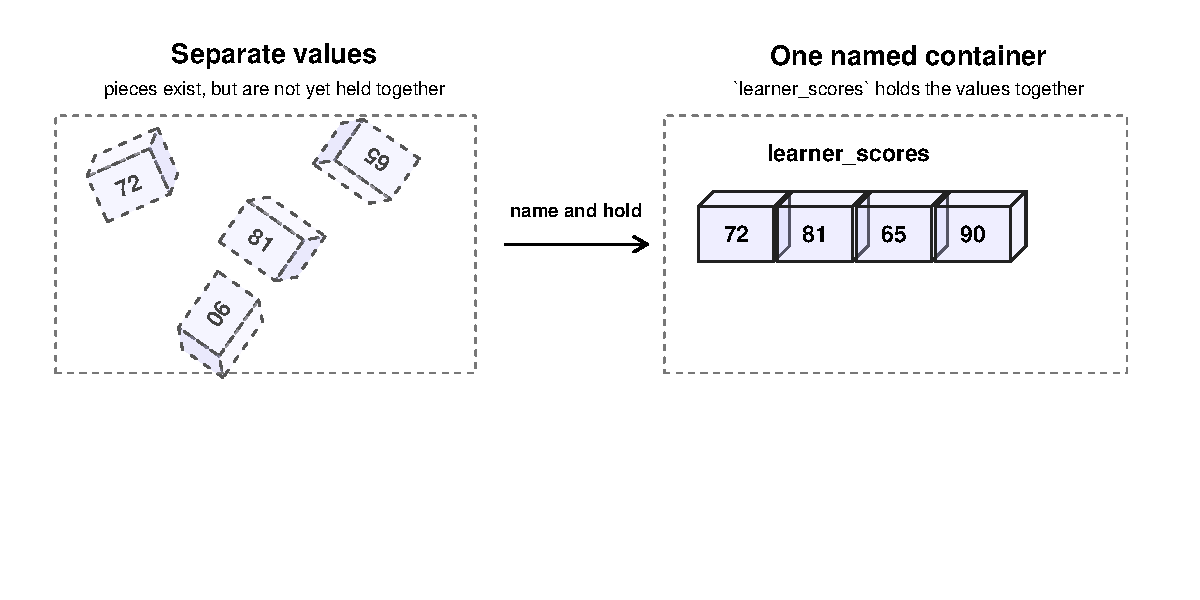
\includegraphics[width=0.9\linewidth,height=\textheight,keepaspectratio]{chapters/03-data-as-atoms-and-containers_files/figure-pdf/fig-learner-scores-container-1.pdf}

}

\caption{\label{fig-learner-scores-container}From Scattered Values to
One Named Container}

\end{figure}%

As shown in Figure~\ref{fig-learner-scores-container}, the point is not
that loose values are wrong. The point is that a name can help R hold
related values together and reuse them.

In this picture, the values \texttt{72}, \texttt{81}, \texttt{65}, and
\texttt{90} first appear as separate pieces. Once they are held under
the name \texttt{learner\_scores}, they become easier to refer to as one
connected object. Later, \href{05-data-structures.qmd}{Chapter 5} will
explain the formal structures behind this idea. For now, the important
lesson is simple: one name can point to more than one piece of data.

The name \texttt{learner\_scores} points to several connected values.
Each value sits in its own cell, but the container allows R to hold the
values together and use them again. Later,
\href{05-data-structures.qmd}{Chapter 5} will explain the formal
structures behind this idea. For now, the important lesson is simple:
one name can point to more than one piece of data.

\begin{Shaded}
\begin{Highlighting}[]
\NormalTok{single value}
\NormalTok{   ↓}
\NormalTok{named object}
\NormalTok{   ↓}
\NormalTok{several connected values}
\NormalTok{   ↓}
\NormalTok{larger data work}
\end{Highlighting}
\end{Shaded}

That map helps prevent a common beginner mistake. Code is not just
symbols on the screen. It is a set of instructions acting on values that
R can find, hold, and inspect.

\section{Special Values Are Still
Signals}\label{special-values-are-still-signals}

Not every value looks like an ordinary number or word.

Real data work contains gaps, impossible calculations, infinite results,
and absence. R has special signals for some of these situations.

The most important ones at this stage are:

\begin{itemize}
\tightlist
\item
  \texttt{NA}
\item
  \texttt{NaN}
\item
  \texttt{Inf}
\item
  \texttt{NULL}
\end{itemize}

These are not decorative details. They matter because serious data work
depends on knowing when a value is present, missing, impossible,
infinite, or absent.

A beginner who ignores special values may trust results too quickly.

\section{Predict Before You Run}\label{predict-before-you-run}

Before running the next code, pause and predict which checks will return
\texttt{TRUE}.

\begin{Shaded}
\begin{Highlighting}[]
\FunctionTok{is.na}\NormalTok{(}\ConstantTok{NA}\NormalTok{)}
\CommentTok{\#\textgreater{} [1] TRUE}
\FunctionTok{is.nan}\NormalTok{(}\ConstantTok{NaN}\NormalTok{)}
\CommentTok{\#\textgreater{} [1] TRUE}
\FunctionTok{is.infinite}\NormalTok{(}\ConstantTok{Inf}\NormalTok{)}
\CommentTok{\#\textgreater{} [1] TRUE}
\FunctionTok{is.null}\NormalTok{(}\ConstantTok{NULL}\NormalTok{)}
\CommentTok{\#\textgreater{} [1] TRUE}
\end{Highlighting}
\end{Shaded}

The purpose is not to memorise these functions immediately. The purpose
is to practise inspection before trust.

R can check what kind of signal it is seeing. The reader should learn to
ask R for evidence rather than guessing.

\section{Missing, Impossible, Infinite, and
Empty}\label{missing-impossible-infinite-and-empty}

\texttt{NA} means a value is missing.

It often appears when a value was expected but is not available.

\begin{Shaded}
\begin{Highlighting}[]
\NormalTok{age }\OtherTok{\textless{}{-}} \ConstantTok{NA}
\FunctionTok{is.na}\NormalTok{(age)}
\CommentTok{\#\textgreater{} [1] TRUE}
\end{Highlighting}
\end{Shaded}

\texttt{NaN} means ``not a number.''

It usually appears when a numerical calculation has produced an
undefined result.

\begin{Shaded}
\begin{Highlighting}[]
\NormalTok{not\_a\_number }\OtherTok{\textless{}{-}} \DecValTok{0} \SpecialCharTok{/} \DecValTok{0}
\NormalTok{not\_a\_number}
\CommentTok{\#\textgreater{} [1] NaN}
\FunctionTok{is.nan}\NormalTok{(not\_a\_number)}
\CommentTok{\#\textgreater{} [1] TRUE}
\end{Highlighting}
\end{Shaded}

\texttt{Inf} means infinity.

It can appear when a calculation produces a value beyond ordinary finite
limits.

\begin{Shaded}
\begin{Highlighting}[]
\NormalTok{infinite\_value }\OtherTok{\textless{}{-}} \DecValTok{1} \SpecialCharTok{/} \DecValTok{0}
\NormalTok{infinite\_value}
\CommentTok{\#\textgreater{} [1] Inf}
\FunctionTok{is.infinite}\NormalTok{(infinite\_value)}
\CommentTok{\#\textgreater{} [1] TRUE}
\end{Highlighting}
\end{Shaded}

\texttt{NULL} needs special care.

It is not a missing value inside a column in the same ordinary way that
\texttt{NA} is. \texttt{NA} usually means a value was expected but is
missing. \texttt{NULL} usually means there is nothing there: no value,
no component, or no object content in that place.

\begin{Shaded}
\begin{Highlighting}[]
\NormalTok{empty\_value }\OtherTok{\textless{}{-}} \ConstantTok{NULL}
\FunctionTok{is.null}\NormalTok{(empty\_value)}
\CommentTok{\#\textgreater{} [1] TRUE}
\end{Highlighting}
\end{Shaded}

This distinction will become more useful later. For now, it is enough to
keep the idea clear:

{\def\LTcaptype{none} % do not increment counter
\begin{longtable}[]{@{}
  >{\raggedright\arraybackslash}p{(\linewidth - 4\tabcolsep) * \real{0.3333}}
  >{\raggedright\arraybackslash}p{(\linewidth - 4\tabcolsep) * \real{0.3333}}
  >{\raggedright\arraybackslash}p{(\linewidth - 4\tabcolsep) * \real{0.3333}}@{}}
\toprule\noalign{}
\begin{minipage}[b]{\linewidth}\raggedright
Signal
\end{minipage} & \begin{minipage}[b]{\linewidth}\raggedright
What it usually means
\end{minipage} & \begin{minipage}[b]{\linewidth}\raggedright
Plain reading
\end{minipage} \\
\midrule\noalign{}
\endhead
\bottomrule\noalign{}
\endlastfoot
\texttt{NA} & A value was expected but is missing & ``Something should
be here, but it is unavailable.'' \\
\texttt{NaN} & A numerical result is undefined & ``This calculation did
not produce a valid number.'' \\
\texttt{Inf} & A numerical result is infinite & ``This value goes beyond
ordinary finite limits.'' \\
\texttt{NULL} & No value or content is present & ``There is nothing
here.'' \\
\end{longtable}
}

\section{Why Inspection Comes Before
Trust}\label{why-inspection-comes-before-trust}

A printed result can look simple while hiding an important signal.

\begin{Shaded}
\begin{Highlighting}[]
\NormalTok{printed result}
\NormalTok{   ↓}
\NormalTok{hidden signal?}
\NormalTok{   ↓}
\NormalTok{inspect before trust}
\end{Highlighting}
\end{Shaded}

For example:

\begin{Shaded}
\begin{Highlighting}[]
\NormalTok{scores\_with\_missing }\OtherTok{\textless{}{-}} \FunctionTok{c}\NormalTok{(}\DecValTok{72}\NormalTok{, }\DecValTok{81}\NormalTok{, }\ConstantTok{NA}\NormalTok{, }\DecValTok{90}\NormalTok{)}
\NormalTok{scores\_with\_missing}
\CommentTok{\#\textgreater{} [1] 72 81 NA 90}
\end{Highlighting}
\end{Shaded}

The missing value may look like a small detail. It is not small when
calculation begins.

\begin{Shaded}
\begin{Highlighting}[]
\FunctionTok{mean}\NormalTok{(scores\_with\_missing)}
\CommentTok{\#\textgreater{} [1] NA}
\end{Highlighting}
\end{Shaded}

R returns \texttt{NA} because one of the values is missing. This is not
a failure in R's behaviour. It is evidence about the data.

R can calculate the mean only when the missing value is handled
deliberately.

\begin{Shaded}
\begin{Highlighting}[]
\FunctionTok{mean}\NormalTok{(scores\_with\_missing, }\AttributeTok{na.rm =} \ConstantTok{TRUE}\NormalTok{)}
\CommentTok{\#\textgreater{} [1] 81}
\end{Highlighting}
\end{Shaded}

This command does not ``fix'' the missing value. It tells R to remove
missing values before calculation.

This small example introduces a professional habit:

\begin{quote}
inspect the material before trusting the result.
\end{quote}

\begin{tcolorbox}[enhanced jigsaw, arc=.35mm, bottomrule=.15mm, breakable, colback=white, colframe=quarto-callout-important-color-frame, left=2mm, leftrule=.75mm, opacityback=0, rightrule=.15mm, toprule=.15mm]
\begin{minipage}[t]{5.5mm}
\textcolor{quarto-callout-important-color}{\faExclamation}
\end{minipage}%
\begin{minipage}[t]{\textwidth - 5.5mm}

\vspace{-3mm}\textbf{Workflow Principle}\vspace{3mm}

A result is only as trustworthy as the data signals that produced it.

\end{minipage}%
\end{tcolorbox}

\section{Why This Matters Before Data
Types}\label{why-this-matters-before-data-types}

It may be tempting to jump straight into formal labels: numeric,
character, logical, and so on.

That will come next.

But a learner who jumps to labels too quickly may miss the deeper idea.
R is not only storing categories of data. It is working with pieces,
names, simple containers, and signals.

The question in Chapter 3 is not yet:

\begin{quote}
What type of data is this?
\end{quote}

The question is:

\begin{quote}
What is the piece of data, where is it being held, and what signal is it
giving?
\end{quote}

Once that question is clear, data types become easier to understand.

\section{What Leo Is Expected to Know at This
Point}\label{what-leo-is-expected-to-know-at-this-point-1}

At this point, the learner does not need to know formal data structures.
There is no need yet to master vectors, lists, matrices, data frames,
coercion, factors, or dates.

The expected understanding is smaller and more important:

\begin{itemize}
\tightlist
\item
  R works with values.
\item
  Values can be given names.
\item
  Names help R find values again.
\item
  Several connected values can be held under one name.
\item
  Special values such as \texttt{NA}, \texttt{NaN}, \texttt{Inf}, and
  \texttt{NULL} carry signals.
\item
  Inspection should come before trust.
\end{itemize}

\begin{tcolorbox}[enhanced jigsaw, arc=.35mm, bottomrule=.15mm, breakable, colback=white, colframe=quarto-callout-note-color-frame, left=2mm, leftrule=.75mm, opacityback=0, rightrule=.15mm, toprule=.15mm]
\begin{minipage}[t]{5.5mm}
\textcolor{quarto-callout-note-color}{\faInfo}
\end{minipage}%
\begin{minipage}[t]{\textwidth - 5.5mm}

\vspace{-3mm}\textbf{Not Yet}\vspace{3mm}

This chapter does not teach formal data types or data structures.

It prepares the mental ground for them. Chapter 4 will ask what kind of
values R is holding. Chapter 5 will ask how values can be organised into
larger structures.

\end{minipage}%
\end{tcolorbox}

\section{Chapter Outcome}\label{chapter-outcome-2}

By the end of this chapter, the learner should be able to explain that R
does not work with vague code symbols. It works with values, names,
simple objects, containers, and signals.

The chapter has introduced a small but important change in thinking:

\begin{Shaded}
\begin{Highlighting}[]
\NormalTok{Do not only read the command.}
\NormalTok{Inspect the data beneath the command.}
\end{Highlighting}
\end{Shaded}

That habit will return throughout the book.

\section{Transition to Chapter 4}\label{transition-to-chapter-4}

The question left by Chapter 2 was:

\begin{quote}
What exactly is R working with when it runs code?
\end{quote}

Chapter 3 answered:

\begin{quote}
R works with values, names, containers, and special signals.
\end{quote}

But another question now appears.

If data comes in pieces, what kind of pieces are they?

Some values behave like numbers. Some behave like text. Some behave like
truth signals. Some look like dates. Some appear simple but behave
differently from what the beginner expects.

Chapter 4 begins there.

\begin{tcolorbox}[enhanced jigsaw, arc=.35mm, bottomrule=.15mm, breakable, colback=white, colframe=quarto-callout-tip-color-frame, left=2mm, leftrule=.75mm, opacityback=0, rightrule=.15mm, toprule=.15mm]
\begin{minipage}[t]{5.5mm}
\textcolor{quarto-callout-tip-color}{\faLightbulb}
\end{minipage}%
\begin{minipage}[t]{\textwidth - 5.5mm}

\vspace{-3mm}\textbf{Ready for the Next Question}\vspace{3mm}

Chapter 3 showed that R works with values before it works with larger
datasets.

Chapter 4 asks the next question:

\textbf{what kind of value is R holding, and why do different values
behave differently?}

\end{minipage}%
\end{tcolorbox}

\chapter{Why Values Behave Differently: Data Types and the Hidden
Identity of
Data}\label{why-values-behave-differently-data-types-and-the-hidden-identity-of-data}

\renewcommand{\thefigure}{4.\arabic{figure}}
\setcounter{figure}{0}

\section{Opening Scene: The Value That Looks Right but
Fails}\label{opening-scene-the-value-that-looks-right-but-fails}

Leo types a line that looks harmless.

\begin{Shaded}
\begin{Highlighting}[]
\StringTok{"10"} \SpecialCharTok{+} \DecValTok{5}
\CommentTok{\#\textgreater{} Error in "10" + 5: non{-}numeric argument to binary operator}
\end{Highlighting}
\end{Shaded}

He expects it to work.

The value \texttt{"10"} looks like a number. The value \texttt{5} is a
number. In ordinary reading, adding ten and five does not feel like a
difficult request.

But R refuses.

Then Leo removes the quotation marks and tries again.

\begin{Shaded}
\begin{Highlighting}[]
\DecValTok{10} \SpecialCharTok{+} \DecValTok{5}
\CommentTok{\#\textgreater{} [1] 15}
\end{Highlighting}
\end{Shaded}

This time, R answers immediately.

The visible difference is small. One value is written as \texttt{"10"}.
The other is written as \texttt{10}.

To Leo, they look almost the same. To R, they are different kinds of
values.

That is the problem at the centre of this chapter.

\begin{quote}
Two values can look almost the same to a human reader and behave
completely differently inside R.
\end{quote}

This is not R being stubborn. It is R being precise.

R does not act only on what appears on the screen. R acts on what a
value is.

\begin{tcolorbox}[enhanced jigsaw, arc=.35mm, bottomrule=.15mm, breakable, colback=white, colframe=quarto-callout-note-color-frame, left=2mm, leftrule=.75mm, opacityback=0, rightrule=.15mm, toprule=.15mm]
\begin{minipage}[t]{5.5mm}
\textcolor{quarto-callout-note-color}{\faInfo}
\end{minipage}%
\begin{minipage}[t]{\textwidth - 5.5mm}

\vspace{-3mm}\textbf{Chapter Compass}\vspace{3mm}

This chapter explains why values behave differently in R.

Chapter 3 showed that R works with values, names, containers, and
special signals. Chapter 4 adds the next layer: values have types, and
those types shape what R can safely do with them.

\end{minipage}%
\end{tcolorbox}

\section{What Changed After Chapter
3}\label{what-changed-after-chapter-3}

Chapter 3 helped Leo stop seeing code as symbols floating on the screen.

He learned that R works with pieces of data, that values can be named,
that several values can be held together, and that some values carry
special signals such as \texttt{NA}, \texttt{NaN}, \texttt{Inf}, and
\texttt{NULL}.

Those special signals matter, but they are not ordinary data types in
the same way that numeric, character, and logical values are.

\begin{tcolorbox}[enhanced jigsaw, arc=.35mm, bottomrule=.15mm, breakable, colback=white, colframe=quarto-callout-note-color-frame, left=2mm, leftrule=.75mm, opacityback=0, rightrule=.15mm, toprule=.15mm]
\begin{minipage}[t]{5.5mm}
\textcolor{quarto-callout-note-color}{\faInfo}
\end{minipage}%
\begin{minipage}[t]{\textwidth - 5.5mm}

\vspace{-3mm}\textbf{Special Values Are Not Ordinary Data Types}\vspace{3mm}

\texttt{NA}, \texttt{NaN}, \texttt{Inf}, and \texttt{NULL} are special
signals in R.

\texttt{NA} marks missingness.\\
\texttt{NaN} marks an undefined numerical result.\\
\texttt{Inf} marks infinity.\\
\texttt{NULL} marks absence.

Some of these signals still have underlying storage when R inspects
them, but their main role is not to name an ordinary data type. Their
role is to tell R that something unusual is happening.

\end{minipage}%
\end{tcolorbox}

A new question now becomes unavoidable:

\begin{quote}
Why do values behave differently even when they look similar?
\end{quote}

That question matters because many beginner errors begin here. A value
may look numeric but behave as text. A date may look like a date but
still be stored as character text. A yes/no response may look meaningful
to a reader but fail to behave as a logical value inside R.

\section{The First Confusion}\label{the-first-confusion}

Return to the first surprise.

\begin{Shaded}
\begin{Highlighting}[]
\StringTok{"10"} \SpecialCharTok{+} \DecValTok{5}
\CommentTok{\# Error: non{-}numeric argument to binary operator}
\end{Highlighting}
\end{Shaded}

R does not accept this.

But this works:

\begin{Shaded}
\begin{Highlighting}[]
\DecValTok{10} \SpecialCharTok{+} \DecValTok{5}
\CommentTok{\#\textgreater{} [1] 15}
\end{Highlighting}
\end{Shaded}

The question is no longer simply:

\begin{quote}
What did Leo type?
\end{quote}

The better question is:

\begin{quote}
What did R think Leo typed?
\end{quote}

When Leo writes \texttt{10}, R sees a number.

When he writes \texttt{"10"}, R sees text.

The quotation marks are not decoration. They change how R interprets the
value.

The failure is not random. It is a clue.

\section{The Hidden Difference}\label{the-hidden-difference}

Look closely:

\begin{itemize}
\tightlist
\item
  \texttt{"10"}
\item
  \texttt{10}
\end{itemize}

They look similar, but they are not the same.

\texttt{"10"} is text. It can be printed, pasted, stored as a label, or
combined with other text.

\texttt{10} is numeric. It can be added, subtracted, averaged, compared,
and used in calculations.

R behaves differently because it sees different kinds of values.

\begin{quote}
What Leo sees is the brick. What R uses is the material.
\end{quote}

The brick is the visible value. The material is the type.

A careful analyst does not trust appearance alone. The figure below puts
the difference side by side.

\begin{figure}

\centering{

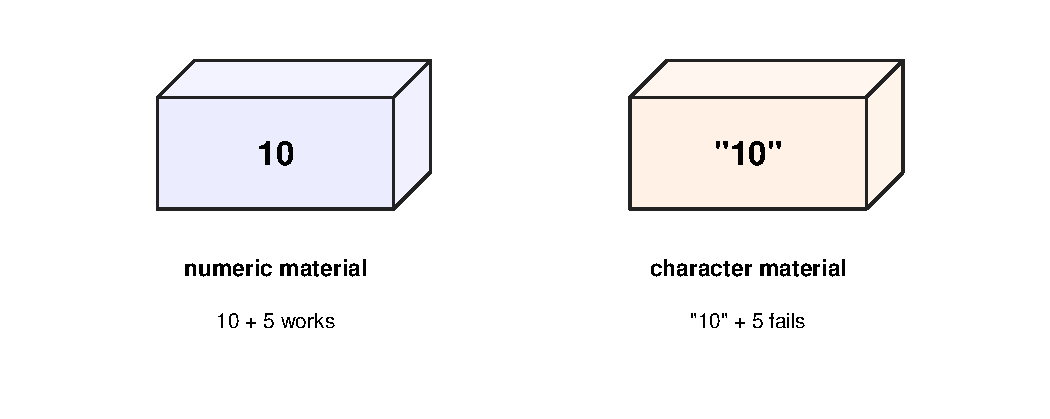
\includegraphics[width=0.9\linewidth,height=\textheight,keepaspectratio]{chapters/04-data-types_files/figure-pdf/fig-same-appearance-different-material-1.pdf}

}

\caption{\label{fig-same-appearance-different-material}Same Appearance,
Different Material}

\end{figure}%

As shown in Figure~\ref{fig-same-appearance-different-material}, the two
values look similar on the screen, but R does not treat them the same
way. The first has numeric material, so arithmetic works. The second has
character material, so arithmetic fails unless the value is deliberately
converted.

This is why Chapter 4 keeps returning to inspection. The screen shows
appearance. Inspection reveals behaviour.

\subsection{The Core Idea: Type Is
Behaviour}\label{the-core-idea-type-is-behaviour}

Every value has a type.

That type helps R decide:

\begin{itemize}
\tightlist
\item
  what the value represents;
\item
  what operations are allowed;
\item
  how the value should behave when a function or operator uses it.
\end{itemize}

A \textbf{data type} is not just a label to memorise. It is part of the
value's behaviour.

When R knows that a value is numeric, it can use that value in
arithmetic. When R knows that a value is character text, it treats that
value as text. When R knows that a value is logical, it can use it in
conditions and checks. When R knows that a value is a date, it can
compare it with other dates and calculate time differences.

So the reliable question is not only:

\begin{quote}
What does this value look like?
\end{quote}

It is:

\begin{quote}
What kind of value does R think this is?
\end{quote}

\begin{tcolorbox}[enhanced jigsaw, arc=.35mm, bottomrule=.15mm, breakable, colback=white, colframe=quarto-callout-tip-color-frame, left=2mm, leftrule=.75mm, opacityback=0, rightrule=.15mm, toprule=.15mm]
\begin{minipage}[t]{5.5mm}
\textcolor{quarto-callout-tip-color}{\faLightbulb}
\end{minipage}%
\begin{minipage}[t]{\textwidth - 5.5mm}

\vspace{-3mm}\textbf{Brick and Material}\vspace{3mm}

In the book's working metaphor:

\begin{itemize}
\tightlist
\item
  the value is the brick;
\item
  the data type is the material of the brick;
\item
  the data structure is how bricks are arranged;
\item
  coercion, later, is what happens when R changes material to make
  values fit together.
\end{itemize}

This chapter is about the material of values. Chapter 5 will ask how
those values are arranged.

\end{minipage}%
\end{tcolorbox}

\section{A Small Example from Everyday
Life}\label{a-small-example-from-everyday-life}

A tuber of yam weighing \texttt{2} kg gives Leo a numeric value. The
value represents a measurable quantity. It can be added to another
weight, compared with another value, or used in calculation.

A football jersey carrying the number \texttt{"10"} is different. The
digits look numeric, but the jersey number functions as a label. Leo
does not usually add jersey numbers as if they were kilograms or exam
scores.

The city name \texttt{"New\ York"} is also character data. It carries
information, but not measurable quantity.

This is why \texttt{"10"} is not always numeric. A value can contain
digit characters and still function as a label.

R needs to know the kind before it can decide what to do.

\section{Seeing Types in Action}\label{seeing-types-in-action}

R gives Leo tools for inspection.

One useful function is \texttt{typeof()}.

\begin{Shaded}
\begin{Highlighting}[]
\FunctionTok{typeof}\NormalTok{(}\StringTok{"10"}\NormalTok{)}
\CommentTok{\#\textgreater{} [1] "character"}
\FunctionTok{typeof}\NormalTok{(}\DecValTok{10}\NormalTok{)}
\CommentTok{\#\textgreater{} [1] "double"}
\end{Highlighting}
\end{Shaded}

The results confirm the hidden difference.

\texttt{"10"} is stored as character text. \texttt{10} is stored as a
numeric value.

Leo does not have to guess. He can ask R what it sees.

That habit matters because visual appearance can mislead him. A value
can look numeric, date-like, or logical without being stored that way. R
will not behave according to Leo's hope. It will behave according to the
value's type.

Some objects also carry a higher-level behaviour label called a
\textbf{class}. That distinction becomes clearer when Leo compares
ordinary values with dates and factors.

For now, the point is simple: R gives Leo ways to inspect a value before
trusting it.

\section{Predict Before You Run}\label{predict-before-you-run-1}

Before moving further, pause and predict what R will see.

Which lines reveal type or class? Which line calculates? Which line
would fail if it were run?

\begin{Shaded}
\begin{Highlighting}[]
\FunctionTok{class}\NormalTok{(}\DecValTok{10}\NormalTok{)}
\FunctionTok{class}\NormalTok{(}\StringTok{"10"}\NormalTok{)}
\DecValTok{10} \SpecialCharTok{+} \DecValTok{5}
\StringTok{"10"} \SpecialCharTok{+} \DecValTok{5}
\end{Highlighting}
\end{Shaded}

Now run the safe inspection lines first.

\begin{Shaded}
\begin{Highlighting}[]
\FunctionTok{class}\NormalTok{(}\DecValTok{10}\NormalTok{)}
\CommentTok{\#\textgreater{} [1] "numeric"}
\FunctionTok{class}\NormalTok{(}\StringTok{"10"}\NormalTok{)}
\CommentTok{\#\textgreater{} [1] "character"}
\end{Highlighting}
\end{Shaded}

Then run the calculation that should work.

\begin{Shaded}
\begin{Highlighting}[]
\DecValTok{10} \SpecialCharTok{+} \DecValTok{5}
\CommentTok{\#\textgreater{} [1] 15}
\end{Highlighting}
\end{Shaded}

The failing line has already appeared at the opening of the chapter.
Here it is only a reminder, so it is shown without running again:

\begin{Shaded}
\begin{Highlighting}[]
\StringTok{"10"} \SpecialCharTok{+} \DecValTok{5}
\CommentTok{\# Error: non{-}numeric argument to binary operator}
\end{Highlighting}
\end{Shaded}

Prediction matters because it turns code reading into reasoning. Leo is
not only waiting for R to answer. He is learning to expect how R should
behave.

\section{Three Behaviours That Reveal
Type}\label{three-behaviours-that-reveal-type}

The easiest way to understand type is to watch values behave.

\subsection{Behaviour 1: Calculation}\label{behaviour-1-calculation}

\begin{Shaded}
\begin{Highlighting}[]
\DecValTok{10} \SpecialCharTok{+} \DecValTok{5}
\CommentTok{\#\textgreater{} [1] 15}
\end{Highlighting}
\end{Shaded}

This works because both values can participate in numeric calculation.
The \texttt{+} operator expects values that can be added, and there is
no conflict.

\subsection{Behaviour 2: Combination}\label{behaviour-2-combination}

\begin{Shaded}
\begin{Highlighting}[]
\FunctionTok{paste}\NormalTok{(}\StringTok{"10"}\NormalTok{, }\DecValTok{5}\NormalTok{)}
\CommentTok{\#\textgreater{} [1] "10 5"}
\end{Highlighting}
\end{Shaded}

This also works, but for a different reason.

\texttt{paste()} combines values as text. It is not trying to perform
arithmetic. It is joining pieces into a character result.

A value that fails in one operation may work in another. The issue is
not whether the value is good or bad. The issue is whether its type fits
the operation being requested.

\subsection{Behaviour 3: Conflict}\label{behaviour-3-conflict}

\begin{Shaded}
\begin{Highlighting}[]
\StringTok{"10"} \SpecialCharTok{+} \DecValTok{5}
\CommentTok{\# Error: non{-}numeric argument to binary operator}
\end{Highlighting}
\end{Shaded}

This fails because the \texttt{+} operator expects numeric values.

The value \texttt{5} is numeric. The value \texttt{"10"} is character
text. R does not treat text as a number simply because it contains digit
characters.

\begin{tcolorbox}[enhanced jigsaw, arc=.35mm, bottomrule=.15mm, breakable, colback=white, colframe=quarto-callout-important-color-frame, left=2mm, leftrule=.75mm, opacityback=0, rightrule=.15mm, toprule=.15mm]
\begin{minipage}[t]{5.5mm}
\textcolor{quarto-callout-important-color}{\faExclamation}
\end{minipage}%
\begin{minipage}[t]{\textwidth - 5.5mm}

\vspace{-3mm}\textbf{Key Insight}\vspace{3mm}

R is not asking whether a value looks like it could work.

R is asking whether the value's type makes the operation valid.

\end{minipage}%
\end{tcolorbox}

\section{Naming the Types}\label{naming-the-types}

Now the names can matter.

Leo has already seen calculation work, text combination work, and type
conflict fail. The labels now explain something he has experienced.

This chapter introduces the kinds of values Leo needs first:

\begin{itemize}
\tightlist
\item
  numeric values
\item
  integer values
\item
  character values
\item
  logical values
\item
  date values
\item
  factor values
\end{itemize}

He does not need to master every detail immediately. The goal is to
recognise the basic type of common values and understand why type
affects behaviour.

{\def\LTcaptype{none} % do not increment counter
\begin{longtable}[]{@{}
  >{\raggedright\arraybackslash}p{(\linewidth - 6\tabcolsep) * \real{0.2500}}
  >{\raggedright\arraybackslash}p{(\linewidth - 6\tabcolsep) * \real{0.2500}}
  >{\raggedright\arraybackslash}p{(\linewidth - 6\tabcolsep) * \real{0.2500}}
  >{\raggedright\arraybackslash}p{(\linewidth - 6\tabcolsep) * \real{0.2500}}@{}}
\toprule\noalign{}
\begin{minipage}[b]{\linewidth}\raggedright
What Leo sees
\end{minipage} & \begin{minipage}[b]{\linewidth}\raggedright
What R may see
\end{minipage} & \begin{minipage}[b]{\linewidth}\raggedright
Beginner meaning
\end{minipage} & \begin{minipage}[b]{\linewidth}\raggedright
Likely behaviour
\end{minipage} \\
\midrule\noalign{}
\endhead
\bottomrule\noalign{}
\endlastfoot
\texttt{10} & numeric/double & A number for calculation & Can be added,
averaged, compared, and measured \\
\texttt{10L} & integer & A whole number stored explicitly as an integer
& Useful for counts, indexes, and whole-number storage \\
\texttt{"10"} & character & Text that happens to contain digit
characters & Behaves like a label, not a quantity \\
\texttt{TRUE} & logical & A truth value & Useful for conditions, checks,
and filtering \\
\texttt{"TRUE"} & character & Text spelling the word TRUE & Looks
logical but behaves like text \\
\texttt{as.Date("2026-04-28")} & Date class & A calendar-aware value &
Can be compared and used in date arithmetic \\
\texttt{factor(c("Beginner",\ "Advanced"))} & factor class & Structured
category labels & Useful for grouping and category-aware work \\
\end{longtable}
}

The same screen can show values that look close to one another, but R
may attach different types or classes to them. Once that happens,
behaviour changes.

\section{Numeric Values}\label{numeric-values}

Numeric values are used for calculation.

They are the ordinary numbers Leo will use for quantities, scores,
measurements, counts, rates, prices, ages, hours, and other measurable
information.

\begin{Shaded}
\begin{Highlighting}[]
\DecValTok{10}
\CommentTok{\#\textgreater{} [1] 10}
\FloatTok{82.5}
\CommentTok{\#\textgreater{} [1] 82.5}
\FunctionTok{typeof}\NormalTok{(}\DecValTok{10}\NormalTok{)}
\CommentTok{\#\textgreater{} [1] "double"}
\FunctionTok{typeof}\NormalTok{(}\FloatTok{82.5}\NormalTok{)}
\CommentTok{\#\textgreater{} [1] "double"}
\end{Highlighting}
\end{Shaded}

Both \texttt{10} and \texttt{82.5} can be used in arithmetic.

\begin{Shaded}
\begin{Highlighting}[]
\DecValTok{10} \SpecialCharTok{+} \FloatTok{82.5}
\CommentTok{\#\textgreater{} [1] 92.5}
\end{Highlighting}
\end{Shaded}

They can be averaged.

\begin{Shaded}
\begin{Highlighting}[]
\FunctionTok{mean}\NormalTok{(}\FunctionTok{c}\NormalTok{(}\DecValTok{10}\NormalTok{, }\DecValTok{20}\NormalTok{, }\DecValTok{30}\NormalTok{))}
\CommentTok{\#\textgreater{} [1] 20}
\end{Highlighting}
\end{Shaded}

They can be compared.

\begin{Shaded}
\begin{Highlighting}[]
\FloatTok{82.5} \SpecialCharTok{\textgreater{}} \DecValTok{70}
\CommentTok{\#\textgreater{} [1] TRUE}
\end{Highlighting}
\end{Shaded}

But a value is not numeric just because it looks numeric on the screen.

\begin{Shaded}
\begin{Highlighting}[]
\FunctionTok{typeof}\NormalTok{(}\StringTok{"82.5"}\NormalTok{)}
\CommentTok{\#\textgreater{} [1] "character"}
\end{Highlighting}
\end{Shaded}

The digits are visible, but the type is character.

That small difference can change the whole analysis.

\section{Integer Values}\label{integer-values}

Integers are whole-number values.

In everyday language, \texttt{10}, \texttt{25}, and \texttt{100} look
like integers because they do not have decimal parts. In R, Leo can
explicitly ask R to store a whole number as an integer by adding
\texttt{L}.

\begin{Shaded}
\begin{Highlighting}[]
\DecValTok{10}\NormalTok{L}
\CommentTok{\#\textgreater{} [1] 10}
\FunctionTok{typeof}\NormalTok{(}\DecValTok{10}\NormalTok{L)}
\CommentTok{\#\textgreater{} [1] "integer"}
\end{Highlighting}
\end{Shaded}

Compare that with ordinary \texttt{10}.

\begin{Shaded}
\begin{Highlighting}[]
\FunctionTok{typeof}\NormalTok{(}\DecValTok{10}\NormalTok{)}
\CommentTok{\#\textgreater{} [1] "double"}
\end{Highlighting}
\end{Shaded}

R stores ordinary \texttt{10} as a double, which is R's common numeric
storage type for numbers that may include decimals.

Leo does not need to overthink this yet. Most beginner work can continue
comfortably with ordinary numeric values. Some functions and datasets
expect whole-number integers explicitly, so he does not need to obsess
over integers now, but he should recognise them when they appear.

For now, it is enough to know that \texttt{10L} and \texttt{10} are
closely related but not identical in how R stores them.

\section{Character Values}\label{character-values}

Character values are text values.

They are used for names, labels, countries, comments, descriptions,
identifiers, and any value R should treat as text rather than as a
number or logical condition.

\begin{Shaded}
\begin{Highlighting}[]
\StringTok{"Leo"}
\CommentTok{\#\textgreater{} [1] "Leo"}
\StringTok{"Nigeria"}
\CommentTok{\#\textgreater{} [1] "Nigeria"}
\StringTok{"New York"}
\CommentTok{\#\textgreater{} [1] "New York"}
\FunctionTok{typeof}\NormalTok{(}\StringTok{"Leo"}\NormalTok{)}
\CommentTok{\#\textgreater{} [1] "character"}
\end{Highlighting}
\end{Shaded}

Character values must be placed inside quotation marks.

Without quotation marks, R assumes Leo is referring to an object name.

\begin{Shaded}
\begin{Highlighting}[]
\NormalTok{name }\OtherTok{\textless{}{-}} \StringTok{"Leo"}
\NormalTok{name}
\CommentTok{\#\textgreater{} [1] "Leo"}
\end{Highlighting}
\end{Shaded}

Here, \texttt{"Leo"} is the text value. \texttt{name} is the object that
stores it.

If Leo writes \texttt{"country"}, R sees the word as text. If he writes
\texttt{country} without quotation marks, R looks for an object called
\texttt{country}.

Character values can also create problems when numbers are accidentally
stored as text.

\begin{Shaded}
\begin{Highlighting}[]
\FunctionTok{typeof}\NormalTok{(}\StringTok{"10"}\NormalTok{)}
\CommentTok{\#\textgreater{} [1] "character"}
\end{Highlighting}
\end{Shaded}

The digits are visible, but the type is still character. This is why the
football jersey example matters. The number \texttt{"10"} may look
numeric, but it functions as a label.

That is why \texttt{"10"\ +\ 5} fails.

\section{Logical Values}\label{logical-values}

Logical values are truth values.

They can only be \texttt{TRUE} or \texttt{FALSE}.

\begin{Shaded}
\begin{Highlighting}[]
\ConstantTok{TRUE}
\CommentTok{\#\textgreater{} [1] TRUE}
\ConstantTok{FALSE}
\CommentTok{\#\textgreater{} [1] FALSE}
\FunctionTok{typeof}\NormalTok{(}\ConstantTok{TRUE}\NormalTok{)}
\CommentTok{\#\textgreater{} [1] "logical"}
\end{Highlighting}
\end{Shaded}

Logical values help R answer yes-or-no questions.

\begin{Shaded}
\begin{Highlighting}[]
\DecValTok{10} \SpecialCharTok{\textgreater{}} \DecValTok{5}
\CommentTok{\#\textgreater{} [1] TRUE}
\end{Highlighting}
\end{Shaded}

\begin{Shaded}
\begin{Highlighting}[]
\DecValTok{10} \SpecialCharTok{\textless{}} \DecValTok{5}
\CommentTok{\#\textgreater{} [1] FALSE}
\end{Highlighting}
\end{Shaded}

Data analysis often involves conditions:

\begin{itemize}
\tightlist
\item
  Did the learner complete the first script?
\item
  Is the score above 70?
\item
  Is the country Nigeria?
\item
  Is the value missing?
\item
  Did the login happen after the enrolment date?
\end{itemize}

Later, Leo will use logical values for filtering rows, checking
assumptions, and creating new variables.

For now, the key idea is simple: logical values help R represent
conditions that are true or false.

\texttt{TRUE} is not the same as \texttt{"TRUE"}.

\begin{Shaded}
\begin{Highlighting}[]
\FunctionTok{typeof}\NormalTok{(}\ConstantTok{TRUE}\NormalTok{)}
\CommentTok{\#\textgreater{} [1] "logical"}
\FunctionTok{typeof}\NormalTok{(}\StringTok{"TRUE"}\NormalTok{)}
\CommentTok{\#\textgreater{} [1] "character"}
\end{Highlighting}
\end{Shaded}

The first is logical. The second is character text.

Again, appearance is not enough.

\section{Dates as Time-Aware Values}\label{dates-as-time-aware-values}

Dates need careful handling because they can look simple while hiding an
important distinction.

This looks like a date:

\begin{Shaded}
\begin{Highlighting}[]
\StringTok{"2026{-}04{-}28"}
\CommentTok{\#\textgreater{} [1] "2026{-}04{-}28"}
\end{Highlighting}
\end{Shaded}

But to R, it is character text unless Leo converts it into a date value.

\begin{Shaded}
\begin{Highlighting}[]
\FunctionTok{typeof}\NormalTok{(}\StringTok{"2026{-}04{-}28"}\NormalTok{)}
\CommentTok{\#\textgreater{} [1] "character"}
\end{Highlighting}
\end{Shaded}

To make R treat it as a date, Leo can use \texttt{as.Date()}.

\begin{Shaded}
\begin{Highlighting}[]
\NormalTok{enrolment\_date }\OtherTok{\textless{}{-}} \FunctionTok{as.Date}\NormalTok{(}\StringTok{"2026{-}04{-}28"}\NormalTok{)}

\NormalTok{enrolment\_date}
\CommentTok{\#\textgreater{} [1] "2026{-}04{-}28"}
\FunctionTok{class}\NormalTok{(enrolment\_date)}
\CommentTok{\#\textgreater{} [1] "Date"}
\FunctionTok{typeof}\NormalTok{(enrolment\_date)}
\CommentTok{\#\textgreater{} [1] "double"}
\end{Highlighting}
\end{Shaded}

\begin{tcolorbox}[enhanced jigsaw, arc=.35mm, bottomrule=.15mm, breakable, colback=white, colframe=quarto-callout-note-color-frame, left=2mm, leftrule=.75mm, opacityback=0, rightrule=.15mm, toprule=.15mm]
\begin{minipage}[t]{5.5mm}
\textcolor{quarto-callout-note-color}{\faInfo}
\end{minipage}%
\begin{minipage}[t]{\textwidth - 5.5mm}

\vspace{-3mm}\textbf{Storage and Behaviour}\vspace{3mm}

\texttt{typeof(enrolment\_date)} answers a storage question: what basic
material is R using underneath?

\texttt{class(enrolment\_date)} answers a practical behaviour question:
how should R treat this object when functions operate on it?

For dates, storage and behaviour are not the same thing. The object is
stored on a numeric foundation, but R treats it as a calendar date
because its class is \texttt{"Date"}.

\end{minipage}%
\end{tcolorbox}

Leo does not need to go deeply into date internals yet. The practical
point is more important: dates are not just decorative text. When parsed
correctly, they become values R can compare and calculate with.

\begin{Shaded}
\begin{Highlighting}[]
\NormalTok{enrolment\_date }\SpecialCharTok{+} \DecValTok{7}
\CommentTok{\#\textgreater{} [1] "2026{-}05{-}05"}
\end{Highlighting}
\end{Shaded}

R can also compare dates.

\begin{Shaded}
\begin{Highlighting}[]
\NormalTok{first\_login\_date }\OtherTok{\textless{}{-}} \FunctionTok{as.Date}\NormalTok{(}\StringTok{"2026{-}05{-}02"}\NormalTok{)}

\NormalTok{first\_login\_date }\SpecialCharTok{\textgreater{}}\NormalTok{ enrolment\_date}
\CommentTok{\#\textgreater{} [1] TRUE}
\end{Highlighting}
\end{Shaded}

This behaviour is possible because R is no longer treating the value as
ordinary text. It is treating it as a date.

\section{Factors as Category-Aware
Values}\label{factors-as-category-aware-values}

Factors represent categories.

They are useful when values belong to a limited set of groups, such as
beginner and advanced, urban and rural, completed and not completed, or
low, medium, and high.

\begin{Shaded}
\begin{Highlighting}[]
\NormalTok{experience\_level }\OtherTok{\textless{}{-}} \FunctionTok{factor}\NormalTok{(}\FunctionTok{c}\NormalTok{(}\StringTok{"beginner"}\NormalTok{, }\StringTok{"developing"}\NormalTok{, }\StringTok{"confident"}\NormalTok{, }\StringTok{"beginner"}\NormalTok{))}

\NormalTok{experience\_level}
\CommentTok{\#\textgreater{} [1] beginner   developing confident  beginner  }
\CommentTok{\#\textgreater{} Levels: beginner confident developing}
\FunctionTok{class}\NormalTok{(experience\_level)}
\CommentTok{\#\textgreater{} [1] "factor"}
\FunctionTok{typeof}\NormalTok{(experience\_level)}
\CommentTok{\#\textgreater{} [1] "integer"}
\end{Highlighting}
\end{Shaded}

\texttt{class(experience\_level)} says the object is a factor. That
tells R to treat it as categorical data.

\texttt{typeof(experience\_level)} shows that the underlying storage is
integer. Those integers are connected to visible category labels.

One small inspection makes the category memory visible.

\begin{Shaded}
\begin{Highlighting}[]
\FunctionTok{levels}\NormalTok{(experience\_level)}
\CommentTok{\#\textgreater{} [1] "beginner"   "confident"  "developing"}
\end{Highlighting}
\end{Shaded}

Factors remember the possible categories attached to the values. That is
the first behavioural difference to notice.

Leo does not need to master all factor details here. Factors can
surprise beginners later, especially when category order matters or when
text is converted into factors unexpectedly.

For now, the practical idea is enough: factors are special objects that
store category labels in a structured way.

\section{Short Recap: What the Types Are
Doing}\label{short-recap-what-the-types-are-doing}

At this point, Leo has met the first set of materials that R uses for
common values.

{\def\LTcaptype{none} % do not increment counter
\begin{longtable}[]{@{}
  >{\raggedright\arraybackslash}p{(\linewidth - 2\tabcolsep) * \real{0.5000}}
  >{\raggedright\arraybackslash}p{(\linewidth - 2\tabcolsep) * \real{0.5000}}@{}}
\toprule\noalign{}
\begin{minipage}[b]{\linewidth}\raggedright
Kind of value
\end{minipage} & \begin{minipage}[b]{\linewidth}\raggedright
What it helps R do
\end{minipage} \\
\midrule\noalign{}
\endhead
\bottomrule\noalign{}
\endlastfoot
Numeric and integer & Calculate, measure, count, compare, and
summarise \\
Character & Store names, labels, identifiers, and descriptions \\
Logical & Represent \texttt{TRUE} or \texttt{FALSE} conditions \\
Date & Carry calendar meaning after correct parsing \\
Factor & Carry category structure, not just loose text labels \\
\end{longtable}
}

The lesson is not that Leo must memorise every technical detail
immediately. The lesson is that each type gives R a different
permission. Some values can be calculated. Some should be treated as
labels. Some carry time. Some carry category structure.

That is why type shapes what analysis is safe.

\section{Why Type Matters in Real
Work}\label{why-type-matters-in-real-work}

The examples so far have been small on purpose.

Small examples help Leo see the principle before he meets the full
dataset.

But this principle will matter every time Leo works with
\texttt{df\_r\_migration}, the book's main dataset.

For example:

\begin{itemize}
\tightlist
\item
  \texttt{study\_hours} should behave like a number when stored
  correctly;
\item
  \texttt{country} may behave like text or as a category, depending on
  the task;
\item
  \texttt{first\_script\_completed} should behave like \texttt{TRUE} or
  \texttt{FALSE} when cleaned properly;
\item
  \texttt{enrolment\_date} and \texttt{first\_login\_date} should behave
  like dates when parsed correctly.
\end{itemize}

These variables are not interchangeable.

Leo should not calculate an average country. He should not paste dates
together when he needs to compare time. He should not treat
\texttt{"TRUE"} as the same thing as \texttt{TRUE}. He should not assume
that a column is numeric just because the values look like numbers.

Type matters because it determines what R can do safely. When Leo
imports a dataset, one of his first tasks is not to calculate. It is to
inspect.

\section{The Silent Failure Problem}\label{the-silent-failure-problem}

Some type problems announce themselves loudly.

\texttt{"10"\ +\ 5} produces an error. Leo sees the problem immediately.

Other type problems are quieter. They may produce warnings, missing
results, strange summaries, or misleading outputs.

Consider this example:

\begin{Shaded}
\begin{Highlighting}[]
\FunctionTok{mean}\NormalTok{(}\FunctionTok{c}\NormalTok{(}\StringTok{"10"}\NormalTok{, }\StringTok{"20"}\NormalTok{, }\StringTok{"30"}\NormalTok{))}
\CommentTok{\#\textgreater{} Warning in mean.default(c("10", "20", "30")): argument is not numeric or}
\CommentTok{\#\textgreater{} logical: returning NA}
\CommentTok{\#\textgreater{} [1] NA}
\end{Highlighting}
\end{Shaded}

Leo may expect the mean to be \texttt{20}, but the values are character
text.

The function \texttt{mean()} is designed for numeric or logical values.
It cannot calculate an ordinary numeric mean from character text, even
if that text contains digit characters.

\begin{tcolorbox}[enhanced jigsaw, arc=.35mm, bottomrule=.15mm, breakable, colback=white, colframe=quarto-callout-warning-color-frame, left=2mm, leftrule=.75mm, opacityback=0, rightrule=.15mm, toprule=.15mm]
\begin{minipage}[t]{5.5mm}
\textcolor{quarto-callout-warning-color}{\faExclamationTriangle}
\end{minipage}%
\begin{minipage}[t]{\textwidth - 5.5mm}

\vspace{-3mm}\textbf{Common Beginner Trap}\vspace{3mm}

If values look numeric but are stored as text, Leo may trust the
appearance and misunderstand the result.

A column can look ready for calculation and still be the wrong type for
calculation.

\end{minipage}%
\end{tcolorbox}

An obvious error may interrupt Leo, but it also protects him by forcing
attention.

A quiet type problem may let the work continue while the interpretation
becomes weak.

Reliable analysis depends on catching these problems early.

\section{Inspect Before You Trust}\label{inspect-before-you-trust}

Leo needs a simple inspection habit.

Before trusting a value, he should check what R sees.

Three useful tools are:

\begin{itemize}
\tightlist
\item
  \texttt{typeof()}
\item
  \texttt{class()}
\item
  \texttt{str()}
\end{itemize}

Start with a single value.

\begin{Shaded}
\begin{Highlighting}[]
\NormalTok{x }\OtherTok{\textless{}{-}} \StringTok{"10"}

\FunctionTok{typeof}\NormalTok{(x)}
\CommentTok{\#\textgreater{} [1] "character"}
\FunctionTok{class}\NormalTok{(x)}
\CommentTok{\#\textgreater{} [1] "character"}
\FunctionTok{str}\NormalTok{(x)}
\CommentTok{\#\textgreater{}  chr "10"}
\end{Highlighting}
\end{Shaded}

\texttt{typeof()} shows the low-level storage type. It answers: what is
the object made from underneath?

\texttt{class()} shows the higher-level behaviour that many R functions
associate with an object. It answers: how should R treat this object
when functions use it?

\texttt{str()} gives a compact summary of structure, storage, and class
information. It becomes especially useful when Leo works with larger
objects later.

Compare the character value with a date.

\begin{Shaded}
\begin{Highlighting}[]
\NormalTok{x }\OtherTok{\textless{}{-}} \FunctionTok{as.Date}\NormalTok{(}\StringTok{"2026{-}04{-}28"}\NormalTok{)}

\FunctionTok{typeof}\NormalTok{(x)}
\CommentTok{\#\textgreater{} [1] "double"}
\FunctionTok{class}\NormalTok{(x)}
\CommentTok{\#\textgreater{} [1] "Date"}
\FunctionTok{str}\NormalTok{(x)}
\CommentTok{\#\textgreater{}  Date[1:1], format: "2026{-}04{-}28"}
\end{Highlighting}
\end{Shaded}

Here, \texttt{typeof()} and \texttt{class()} do not tell the same story.
That is not a contradiction. It is a layered view.

For dates and factors, storage and behaviour are not always the same
thing.

\begin{tcolorbox}[enhanced jigsaw, arc=.35mm, bottomrule=.15mm, breakable, colback=white, colframe=quarto-callout-note-color-frame, left=2mm, leftrule=.75mm, opacityback=0, rightrule=.15mm, toprule=.15mm]
\begin{minipage}[t]{5.5mm}
\textcolor{quarto-callout-note-color}{\faInfo}
\end{minipage}%
\begin{minipage}[t]{\textwidth - 5.5mm}

\vspace{-3mm}\textbf{Storage and Behaviour}\vspace{3mm}

\texttt{typeof()} answers a storage question.

\texttt{class()} answers a practical behaviour question.

\texttt{str()} gives a compact inspection view.

\end{minipage}%
\end{tcolorbox}

Leo does not need to memorise every possible output. He needs to build
the habit of inspection.

The question is always:

\begin{quote}
What does R see here?
\end{quote}

That question is one of the foundations of careful analysis.

\section{The First Rule of Reliable
Analysis}\label{the-first-rule-of-reliable-analysis}

Here is the rule Leo should keep:

\begin{quote}
Never assume what a value is. Confirm what R sees.
\end{quote}

A fragile analysis begins with assumptions:

\begin{quote}
This looks like a number, so it must be numeric.
\end{quote}

\begin{quote}
This looks like a date, so R must understand it as a date.
\end{quote}

\begin{quote}
This looks like true or false, so it must be logical.
\end{quote}

A reliable analysis begins with inspection.

\begin{Shaded}
\begin{Highlighting}[]
\NormalTok{x }\OtherTok{\textless{}{-}} \StringTok{"10"}

\FunctionTok{typeof}\NormalTok{(x)}
\CommentTok{\#\textgreater{} [1] "character"}
\end{Highlighting}
\end{Shaded}

Then Leo can decide what to do next.

If the value is already numeric, he can calculate. If the value is
character text but should be numeric, he may need to convert it. If the
value is character text and should remain text, he can treat it as text.
If the value is a date written as text, he may need to parse it as a
date.

The rule is not about being slow. It is about being safe.

\begin{tcolorbox}[enhanced jigsaw, arc=.35mm, bottomrule=.15mm, breakable, colback=white, colframe=quarto-callout-important-color-frame, left=2mm, leftrule=.75mm, opacityback=0, rightrule=.15mm, toprule=.15mm]
\begin{minipage}[t]{5.5mm}
\textcolor{quarto-callout-important-color}{\faExclamation}
\end{minipage}%
\begin{minipage}[t]{\textwidth - 5.5mm}

\vspace{-3mm}\textbf{Reliable Analysis Rule}\vspace{3mm}

Never assume what a value is.

Confirm what R sees before trusting what the value appears to be.

\end{minipage}%
\end{tcolorbox}

\section{The Mental Shift}\label{the-mental-shift}

At the beginning of this chapter, Leo's old assumption was
understandable:

\begin{quote}
Values that look similar behave the same.
\end{quote}

That assumption works in ordinary human reading. It does not work safely
in R.

The stronger understanding is:

\begin{quote}
Values behave according to their type, not their appearance.
\end{quote}

\texttt{"10"} and \texttt{10} are not the same because one is character
text and the other is numeric.

\texttt{"TRUE"} and \texttt{TRUE} are not the same because one is
character text and the other is logical.

\texttt{"2026-04-28"} and \texttt{as.Date("2026-04-28")} are not the
same because one is text and the other is a date-aware value.

A factor and a character value may print labels that look similar, but R
can treat them differently because one carries category structure.

Errors stop looking like personal failure. Warnings become signals.
Strange outputs become clues. Inspection becomes part of the work.

R is not being difficult. R is obeying the type of the value.

\section{Leo's Notebook}\label{leos-notebook}

Leo writes the lesson in his own words:

\begin{quote}
A value is not only what it looks like on the screen. A value is what R
understands it to be. Before I calculate, compare, filter, or summarise,
I should check what R sees.
\end{quote}

That note carries the heart of the chapter.

\section{What Comes Next}\label{what-comes-next}

This chapter has focused on individual values.

Leo now understands that every value has a type, and that some objects
also carry a class that guides how R treats them. A number, a piece of
text, a logical value, a date, and a factor may all appear quietly on
the screen, but R does not treat them as interchangeable.

Real analysis rarely works with one value at a time.

Leo will soon work with many values together:

\begin{itemize}
\tightlist
\item
  many scores;
\item
  many learner names;
\item
  many countries;
\item
  many enrolment dates;
\item
  many completion statuses;
\item
  many rows in a dataset.
\end{itemize}

\begin{tcolorbox}[enhanced jigsaw, arc=.35mm, bottomrule=.15mm, breakable, colback=white, colframe=quarto-callout-tip-color-frame, left=2mm, leftrule=.75mm, opacityback=0, rightrule=.15mm, toprule=.15mm]
\begin{minipage}[t]{5.5mm}
\textcolor{quarto-callout-tip-color}{\faLightbulb}
\end{minipage}%
\begin{minipage}[t]{\textwidth - 5.5mm}

\vspace{-3mm}\textbf{Bridge to Data Structures}\vspace{3mm}

A single value has a type.

A group of values needs an arrangement.

That arrangement is where data structures begin.

\end{minipage}%
\end{tcolorbox}

The next chapter will not simply ask how to store many values. It will
ask what happens when values enter containers with rules. Some
containers demand sameness. Some allow mixture. Some are shaped for
calculation. Some are shaped for flexible representation. Some become
the table-like form Leo will rely on throughout the book.

\section{Chapter Outcome}\label{chapter-outcome-3}

By the end of this chapter, Leo can:

\begin{itemize}
\tightlist
\item
  recognise that values can look similar but behave differently;
\item
  explain that type drives behaviour in R;
\item
  use the brick/material metaphor to explain data types;
\item
  distinguish numeric, integer, character, logical, date, and factor
  values at a beginner level;
\item
  understand that dates and factors have special behaviour beyond
  ordinary text;
\item
  explain why \texttt{"10"} and \texttt{10} are not the same value to R;
\item
  detect simple type mismatch problems;
\item
  inspect values using \texttt{typeof()}, \texttt{class()}, and
  \texttt{str()};
\item
  explain the difference between low-level storage type and higher-level
  object class;
\item
  explain why reliable analysis begins by checking what R sees.
\end{itemize}

More importantly, Leo has gained a habit that will protect his work.

He will no longer trust appearance alone.

He will ask R what it sees.

That habit will matter when values are placed inside larger structures,
because a container does not only hold data. It also imposes rules on
how values live together.

Leo now knows that every value has a material. In the next chapter, he
will discover that every container has an arrangement.

\section{Key Terms}\label{key-terms}

\textbf{Value}: One piece of data that R can store, inspect, or use.

\textbf{Data type}: The internal kind of a value. In this chapter's
metaphor, type is the material of the data brick.

\textbf{Numeric}: A value used for calculation, measurement, comparison,
and summary.

\textbf{Integer}: A whole-number value stored explicitly as an integer,
often written with \texttt{L}, as in \texttt{10L}.

\textbf{Character}: Text data, usually written inside quotation marks.

\textbf{Logical}: A truth value, either \texttt{TRUE} or \texttt{FALSE}.

\textbf{Date}: A calendar-aware value created when date-like text is
parsed correctly, often with \texttt{as.Date()}.

\textbf{Factor}: A structured category value that stores category labels
in a way R can use for category-aware work.

\textbf{\texttt{typeof()}}: A function that shows the low-level storage
type of an object.

\textbf{\texttt{class()}}: A function that shows the higher-level
behaviour R associates with an object.

\textbf{\texttt{str()}}: A function that gives a compact view of an
object's structure, type, and class information.

\section{Practice Lab}\label{practice-lab}

This lab helps Leo turn the chapter's ideas into action.

\subsection{Task 1: Compare what looks
similar}\label{task-1-compare-what-looks-similar}

Run the code below.

\begin{Shaded}
\begin{Highlighting}[]
\FunctionTok{typeof}\NormalTok{(}\StringTok{"10"}\NormalTok{)}
\CommentTok{\#\textgreater{} [1] "character"}
\FunctionTok{typeof}\NormalTok{(}\DecValTok{10}\NormalTok{)}
\CommentTok{\#\textgreater{} [1] "double"}

\FunctionTok{class}\NormalTok{(}\StringTok{"10"}\NormalTok{)}
\CommentTok{\#\textgreater{} [1] "character"}
\FunctionTok{class}\NormalTok{(}\DecValTok{10}\NormalTok{)}
\CommentTok{\#\textgreater{} [1] "numeric"}
\end{Highlighting}
\end{Shaded}

Then answer:

\begin{itemize}
\tightlist
\item
  Why does \texttt{"10"} behave differently from \texttt{10}?
\item
  Which one is safe for arithmetic?
\item
  Which one behaves like text?
\end{itemize}

\subsection{Task 2: Inspect truth
values}\label{task-2-inspect-truth-values}

Run the code below.

\begin{Shaded}
\begin{Highlighting}[]
\FunctionTok{typeof}\NormalTok{(}\ConstantTok{TRUE}\NormalTok{)}
\CommentTok{\#\textgreater{} [1] "logical"}
\FunctionTok{typeof}\NormalTok{(}\StringTok{"TRUE"}\NormalTok{)}
\CommentTok{\#\textgreater{} [1] "character"}

\FunctionTok{class}\NormalTok{(}\ConstantTok{TRUE}\NormalTok{)}
\CommentTok{\#\textgreater{} [1] "logical"}
\FunctionTok{class}\NormalTok{(}\StringTok{"TRUE"}\NormalTok{)}
\CommentTok{\#\textgreater{} [1] "character"}
\end{Highlighting}
\end{Shaded}

Then answer:

\begin{itemize}
\tightlist
\item
  Why is \texttt{TRUE} different from \texttt{"TRUE"}?
\item
  Which one can help R make a logical decision?
\end{itemize}

\subsection{Task 3: Inspect dates and
categories}\label{task-3-inspect-dates-and-categories}

Run the code below.

\begin{Shaded}
\begin{Highlighting}[]
\NormalTok{login\_date }\OtherTok{\textless{}{-}} \FunctionTok{as.Date}\NormalTok{(}\StringTok{"2026{-}04{-}28"}\NormalTok{)}
\NormalTok{experience\_level }\OtherTok{\textless{}{-}} \FunctionTok{factor}\NormalTok{(}\FunctionTok{c}\NormalTok{(}\StringTok{"beginner"}\NormalTok{, }\StringTok{"developing"}\NormalTok{, }\StringTok{"confident"}\NormalTok{, }\StringTok{"beginner"}\NormalTok{))}

\FunctionTok{typeof}\NormalTok{(login\_date)}
\CommentTok{\#\textgreater{} [1] "double"}
\FunctionTok{class}\NormalTok{(login\_date)}
\CommentTok{\#\textgreater{} [1] "Date"}
\FunctionTok{str}\NormalTok{(login\_date)}
\CommentTok{\#\textgreater{}  Date[1:1], format: "2026{-}04{-}28"}

\FunctionTok{typeof}\NormalTok{(experience\_level)}
\CommentTok{\#\textgreater{} [1] "integer"}
\FunctionTok{class}\NormalTok{(experience\_level)}
\CommentTok{\#\textgreater{} [1] "factor"}
\FunctionTok{levels}\NormalTok{(experience\_level)}
\CommentTok{\#\textgreater{} [1] "beginner"   "confident"  "developing"}
\FunctionTok{str}\NormalTok{(experience\_level)}
\CommentTok{\#\textgreater{}  Factor w/ 3 levels "beginner","confident",..: 1 3 2 1}
\end{Highlighting}
\end{Shaded}

Then answer:

\begin{itemize}
\tightlist
\item
  What does \texttt{typeof()} show for the date?
\item
  What does \texttt{class()} show for the date?
\item
  What does \texttt{class()} show for the factor?
\item
  What does \texttt{levels()} reveal about the factor?
\item
  Why do \texttt{typeof()} and \texttt{class()} not always tell the same
  story?
\end{itemize}

\subsection{Task 4: Write the lesson in plain
language}\label{task-4-write-the-lesson-in-plain-language}

Complete these sentences in your own words:

\begin{Shaded}
\begin{Highlighting}[]
\NormalTok{A data type tells R...}

\NormalTok{The difference between typeof() and class() is...}

\NormalTok{Before I trust a value, I should...}
\end{Highlighting}
\end{Shaded}

The goal is not to memorise the terms. The goal is to build the habit:
inspect first, then analyse.

\chapter{How Data Holds Together: Structures, Containers, and the Shape
of R
Work}\label{how-data-holds-together-structures-containers-and-the-shape-of-r-work}

\renewcommand{\thefigure}{5.\arabic{figure}}
\setcounter{figure}{0}

\section{Opening Scene: When One Value Becomes
Many}\label{opening-scene-when-one-value-becomes-many}

Leo has just crossed an important bridge.

He now understands why \texttt{"10"} and \texttt{10} do not behave the
same way in R. One is text. The other is a number. They may look similar
on the screen, but R does not judge values by appearance alone. R also
asks what kind of value each one is.

That was the lesson of Chapter 4.

But real analysis does not stop with one value.

A dataset contains many values at once: scores, names, dates, countries,
categories, true-or-false indicators, and repeated observations. One
learner record may contain a name as text, study hours as a number, a
completion status as a logical value, and an enrolment date as a
calendar-aware value. These values are different, but they still belong
together.

So a new question appears:

\begin{quote}
If every value has a type, what happens when many values must live
together?
\end{quote}

This is where R becomes more than a place that stores values. It becomes
a system for organising them.

A single value is easy to inspect. Many values need order. Without
order, R cannot know which values form a variable, which values form a
record, which values can be calculated together, or which values should
remain separate.

R therefore needs more than values.

It needs structures.

\section{What Changed After Chapter
4}\label{what-changed-after-chapter-4}

By the end of Chapter 4, Leo understood that data is not only what
appears on the screen. A value has a type, and that type affects what R
can safely do with it.

He learned that:

\begin{itemize}
\tightlist
\item
  R works with data.
\item
  Data begins as small pieces.
\item
  Each piece has a type.
\item
  Type influences behaviour.
\item
  Values that look similar may behave differently.
\end{itemize}

That understanding was still focused on individual values.

Chapter 5 adds the next layer. A single value has a type, but a group of
values also needs an arrangement. That arrangement is the structure.

\begin{tcolorbox}[enhanced jigsaw, arc=.35mm, bottomrule=.15mm, breakable, colback=white, colframe=quarto-callout-note-color-frame, left=2mm, leftrule=.75mm, opacityback=0, rightrule=.15mm, toprule=.15mm]
\begin{minipage}[t]{5.5mm}
\textcolor{quarto-callout-note-color}{\faInfo}
\end{minipage}%
\begin{minipage}[t]{\textwidth - 5.5mm}

\vspace{-3mm}\textbf{Chapter Compass}\vspace{3mm}

In this chapter, Leo learns why R needs data structures, how structures
organise values, and why vectors, lists, matrices, and data frames
behave differently.

The central idea is simple:

\begin{quote}
Type explains how one value behaves. Structure explains how many values
behave together.
\end{quote}

\end{minipage}%
\end{tcolorbox}

\section{Why Structure Matters}\label{why-structure-matters}

Suppose Leo records the scores of four learners.

\begin{Shaded}
\begin{Highlighting}[]
\DecValTok{70}
\CommentTok{\#\textgreater{} [1] 70}
\DecValTok{82}
\CommentTok{\#\textgreater{} [1] 82}
\DecValTok{91}
\CommentTok{\#\textgreater{} [1] 91}
\DecValTok{64}
\CommentTok{\#\textgreater{} [1] 64}
\end{Highlighting}
\end{Shaded}

Each number is meaningful. But as separate values, they are not yet a
useful analytical object. R can print them one after another, but it has
not been told that they belong together as a set of scores.

Leo does not want four isolated numbers. He wants a collection he can
calculate with, inspect, sort, compare, and connect to learner records.

That requires structure.

The same problem appears in every real dataset. A researcher may have
many learner names. A public health analyst may have many dates. A
migration researcher may have many countries. A teacher may have many
assessment records. A business analyst may have many transactions across
time.

In each case, R must organise values so it can:

\begin{itemize}
\tightlist
\item
  store them;
\item
  access them;
\item
  process them;
\item
  compare them;
\item
  transform them;
\item
  preserve relationships among them.
\end{itemize}

That organisation is called a \textbf{data structure}.

A data structure is not just a place where values are kept. It is a
rule-governed arrangement that tells R how values belong together.

\section{Containers Become
Structures}\label{containers-become-structures}

In Chapter 3, Leo met containers as a beginner's mental model: a way to
imagine more than one value being held together.

Chapter 5 makes that idea more precise.

\begin{quote}
A data structure is a defined way R organises values inside a container.
\end{quote}

The word \textbf{defined} matters.

A structure is not an empty basket where anything can be dropped without
consequence. Each structure has rules. Those rules affect what can go
inside, how values are stored, how values are accessed, and what R can
do with them.

This is why two objects may both hold data but behave differently. One
structure may demand that all its values share one type. Another may
allow different types to remain different. One may behave like a simple
line of values. Another may behave like a table.

\begin{tcolorbox}[enhanced jigsaw, arc=.35mm, bottomrule=.15mm, breakable, colback=white, colframe=quarto-callout-tip-color-frame, left=2mm, leftrule=.75mm, opacityback=0, rightrule=.15mm, toprule=.15mm]
\begin{minipage}[t]{5.5mm}
\textcolor{quarto-callout-tip-color}{\faLightbulb}
\end{minipage}%
\begin{minipage}[t]{\textwidth - 5.5mm}

\vspace{-3mm}\textbf{Core Mental Model}\vspace{3mm}

A value is the brick.

A type is the material.

A structure is the arrangement.

\end{minipage}%
\end{tcolorbox}

\section{A Small Visual Map of
Structures}\label{a-small-visual-map-of-structures}

Before Leo studies each structure in detail, he needs a first map of the
territory.

The figure below is not a full technical definition. It is a mental
picture of arrangement: one line, rows and columns, mixed components,
and table-like columns.

\begin{figure}

\centering{

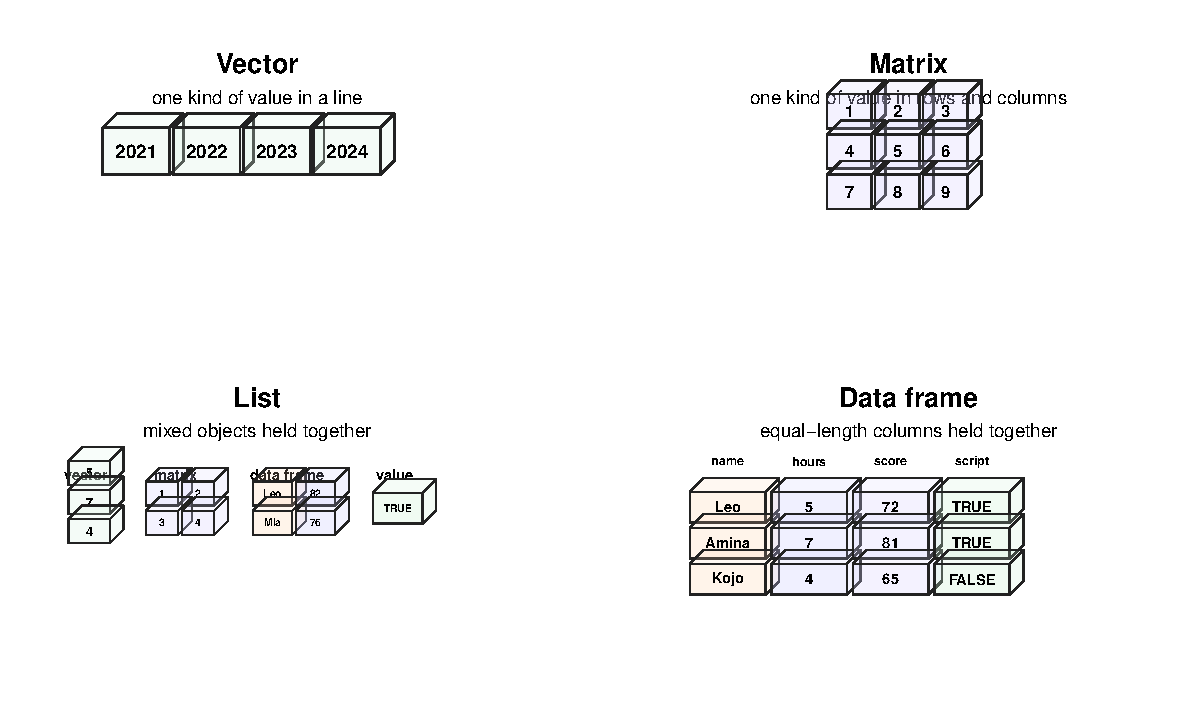
\includegraphics[width=0.9\linewidth,height=\textheight,keepaspectratio]{chapters/05-data-structures_files/figure-pdf/fig-four-data-structures-1.pdf}

}

\caption{\label{fig-four-data-structures}Four Ways Values Can Be
Arranged}

\end{figure}%

As shown in Figure~\ref{fig-four-data-structures}, the same idea of
``holding values together'' can take different shapes. A vector keeps
one kind of value in a line. Here, the vector contains year values. A
matrix still keeps one kind of value, but arranges it into rows and
columns. A list can hold mixed objects together, including a vector, a
matrix, a small data frame, and a single value. A data frame holds
equal-length columns together as a table, which is why it becomes
central to real data work.

The figure is only a map. The next sections explain each structure
slowly, starting with the two behaviours Leo needs to recognise before
the structure names become meaningful.

\section{The Two Behaviours Every Beginner Should
Notice}\label{the-two-behaviours-every-beginner-should-notice}

Before Leo memorises the names of R structures, he needs to notice a
deeper pattern.

Some structures enforce sameness. Others preserve difference.

A structure that enforces sameness is called \textbf{homogeneous}. A
structure that preserves different kinds of values is called
\textbf{heterogeneous}.

A homogeneous structure says:

\begin{quote}
Values inside this structure must follow one type rule.
\end{quote}

A heterogeneous structure says:

\begin{quote}
Related values may remain different and still belong together.
\end{quote}

This distinction explains why a vector behaves differently from a list,
why a matrix is stricter than a data frame, and why R sometimes changes
values in ways that surprise beginners.

\section{Homogeneous Structures: When Sameness
Matters}\label{homogeneous-structures-when-sameness-matters}

A homogeneous structure requires a shared type rule.

Homogeneous structures are useful when Leo is working with uniform data,
such as:

\begin{itemize}
\tightlist
\item
  a set of scores;
\item
  a set of distances;
\item
  a set of logical responses;
\item
  a set of text labels.
\end{itemize}

The strength of this structure is consistency. If R knows a structure is
numeric throughout, functions such as \texttt{mean()}, \texttt{sum()},
and \texttt{max()} can operate with confidence.

Sameness is not a limitation here. It is the condition that makes
certain operations safe.

\section{The First Homogeneous Structure:
Vector}\label{the-first-homogeneous-structure-vector}

The simplest common data structure in R is the \textbf{vector}.

A vector holds multiple values in a single ordered structure. Leo can
create a vector of scores using \texttt{c()}, which combines values.

\begin{Shaded}
\begin{Highlighting}[]
\NormalTok{scores }\OtherTok{\textless{}{-}} \FunctionTok{c}\NormalTok{(}\DecValTok{70}\NormalTok{, }\DecValTok{82}\NormalTok{, }\DecValTok{91}\NormalTok{, }\DecValTok{64}\NormalTok{)}
\NormalTok{scores}
\CommentTok{\#\textgreater{} [1] 70 82 91 64}
\end{Highlighting}
\end{Shaded}

This object now holds four values together.

They are not four separate numbers sitting loosely on the screen. They
are one structured object named \texttt{scores}.

Because the values are numeric and belong together, Leo can calculate
with them easily.

\begin{Shaded}
\begin{Highlighting}[]
\FunctionTok{mean}\NormalTok{(scores)}
\CommentTok{\#\textgreater{} [1] 76.75}
\end{Highlighting}
\end{Shaded}

The calculation works smoothly because the values inside \texttt{scores}
share a common type. They are all numbers, and the structure is designed
for that kind of uniformity.

The vector is also ordered. The first value is \texttt{70}, the second
is \texttt{82}, the third is \texttt{91}, and the fourth is \texttt{64}.
This order means R can access values by position.

\begin{Shaded}
\begin{Highlighting}[]
\NormalTok{scores[}\DecValTok{1}\NormalTok{]}
\CommentTok{\#\textgreater{} [1] 70}
\end{Highlighting}
\end{Shaded}

The result is the first value in the vector.

At this point, Leo has learned something small but powerful: R is not
just storing four scores. It is storing them in a structure that makes
calculation and selection possible.

\subsection{Vectors can hold different kinds of uniform
data}\label{vectors-can-hold-different-kinds-of-uniform-data}

The first example used numbers because numeric vectors are easy to
calculate with. But a vector does not have to be numeric.

A vector can hold different kinds of data, as long as one atomic vector
keeps one type rule.

Leo can create a character vector of countries.

\begin{Shaded}
\begin{Highlighting}[]
\NormalTok{countries }\OtherTok{\textless{}{-}} \FunctionTok{c}\NormalTok{(}\StringTok{"Nigeria"}\NormalTok{, }\StringTok{"Ghana"}\NormalTok{, }\StringTok{"Kenya"}\NormalTok{, }\StringTok{"South Africa"}\NormalTok{)}
\NormalTok{countries}
\CommentTok{\#\textgreater{} [1] "Nigeria"      "Ghana"        "Kenya"        "South Africa"}
\FunctionTok{typeof}\NormalTok{(countries)}
\CommentTok{\#\textgreater{} [1] "character"}
\end{Highlighting}
\end{Shaded}

This vector is still homogeneous. Its values are all character values.

He can also create a logical vector.

\begin{Shaded}
\begin{Highlighting}[]
\NormalTok{completed }\OtherTok{\textless{}{-}} \FunctionTok{c}\NormalTok{(}\ConstantTok{TRUE}\NormalTok{, }\ConstantTok{TRUE}\NormalTok{, }\ConstantTok{FALSE}\NormalTok{, }\ConstantTok{TRUE}\NormalTok{)}
\NormalTok{completed}
\CommentTok{\#\textgreater{} [1]  TRUE  TRUE FALSE  TRUE}
\FunctionTok{typeof}\NormalTok{(completed)}
\CommentTok{\#\textgreater{} [1] "logical"}
\end{Highlighting}
\end{Shaded}

This vector is homogeneous too. Its values all carry truth-or-false
meaning.

Dates can also live in a vector, although dates need both storage and
class information.

\begin{Shaded}
\begin{Highlighting}[]
\NormalTok{login\_dates }\OtherTok{\textless{}{-}} \FunctionTok{as.Date}\NormalTok{(}\FunctionTok{c}\NormalTok{(}\StringTok{"2026{-}04{-}01"}\NormalTok{, }\StringTok{"2026{-}04{-}03"}\NormalTok{, }\StringTok{"2026{-}04{-}08"}\NormalTok{))}
\NormalTok{login\_dates}
\CommentTok{\#\textgreater{} [1] "2026{-}04{-}01" "2026{-}04{-}03" "2026{-}04{-}08"}
\FunctionTok{typeof}\NormalTok{(login\_dates)}
\CommentTok{\#\textgreater{} [1] "double"}
\FunctionTok{class}\NormalTok{(login\_dates)}
\CommentTok{\#\textgreater{} [1] "Date"}
\end{Highlighting}
\end{Shaded}

The underlying storage is not the whole story here. \texttt{typeof()}
shows the lower-level storage, while \texttt{class()} tells Leo that R
should treat the values as dates. This connects back to Chapter 4:
sometimes R needs more than the raw storage type to know how a value
should behave.

Factors also behave as structured categorical vectors.

\begin{Shaded}
\begin{Highlighting}[]
\NormalTok{r\_experience\_level }\OtherTok{\textless{}{-}} \FunctionTok{factor}\NormalTok{(}\FunctionTok{c}\NormalTok{(}\StringTok{"beginner"}\NormalTok{, }\StringTok{"developing"}\NormalTok{, }\StringTok{"beginner"}\NormalTok{, }\StringTok{"confident"}\NormalTok{))}
\NormalTok{r\_experience\_level}
\CommentTok{\#\textgreater{} [1] beginner   developing beginner   confident }
\CommentTok{\#\textgreater{} Levels: beginner confident developing}
\FunctionTok{typeof}\NormalTok{(r\_experience\_level)}
\CommentTok{\#\textgreater{} [1] "integer"}
\FunctionTok{class}\NormalTok{(r\_experience\_level)}
\CommentTok{\#\textgreater{} [1] "factor"}
\end{Highlighting}
\end{Shaded}

A factor is useful when values represent categories. It may print like
words, but internally it carries category structure.

So the deeper point is not that a vector must be numeric. The point is
that a vector is a one-dimensional structure that expects internal
consistency.

\begin{tcolorbox}[enhanced jigsaw, arc=.35mm, bottomrule=.15mm, breakable, colback=white, colframe=quarto-callout-note-color-frame, left=2mm, leftrule=.75mm, opacityback=0, rightrule=.15mm, toprule=.15mm]
\begin{minipage}[t]{5.5mm}
\textcolor{quarto-callout-note-color}{\faInfo}
\end{minipage}%
\begin{minipage}[t]{\textwidth - 5.5mm}

\vspace{-3mm}\textbf{Vector Characteristics}\vspace{3mm}

A vector is:

\begin{itemize}
\tightlist
\item
  one-dimensional;
\item
  ordered;
\item
  usually used for one variable or one kind of information;
\item
  homogeneous when it is an atomic vector;
\item
  accessible by position;
\item
  useful for repeated values such as scores, countries, dates,
  categories, or logical flags.
\end{itemize}

\end{minipage}%
\end{tcolorbox}

Leo can now see why vectors are everywhere in R. A column in a data
frame is usually a vector. That means understanding vectors prepares him
to understand larger data structures later.

\section{When R Forces Values to Fit}\label{when-r-forces-values-to-fit}

The same vector rule that makes numeric calculation easy can also create
surprises.

A vector wants its values to share one type. So what happens if Leo
tries to combine values that do not naturally share the same type?

\begin{Shaded}
\begin{Highlighting}[]
\NormalTok{mixed }\OtherTok{\textless{}{-}} \FunctionTok{c}\NormalTok{(}\DecValTok{10}\NormalTok{, }\StringTok{"Leo"}\NormalTok{, }\ConstantTok{TRUE}\NormalTok{)}
\NormalTok{mixed}
\CommentTok{\#\textgreater{} [1] "10"   "Leo"  "TRUE"}
\end{Highlighting}
\end{Shaded}

Leo intended to combine a number, text, and a logical value. But an
atomic vector cannot preserve different atomic types side by side
without coercion. It must find one common type that can hold all the
values.

He can inspect what happened.

\begin{Shaded}
\begin{Highlighting}[]
\FunctionTok{typeof}\NormalTok{(mixed)}
\CommentTok{\#\textgreater{} [1] "character"}
\end{Highlighting}
\end{Shaded}

R reports that the vector is character.

The number \texttt{10} and the logical value \texttt{TRUE} have been
converted so they can live with \texttt{"Leo"} inside one homogeneous
structure. R has forced consistency.

This behaviour is not random. R is protecting the rule of the structure.
The vector says, in effect, ``If values must live here together, they
must share one type.''

\begin{tcolorbox}[enhanced jigsaw, arc=.35mm, bottomrule=.15mm, breakable, colback=white, colframe=quarto-callout-warning-color-frame, left=2mm, leftrule=.75mm, opacityback=0, rightrule=.15mm, toprule=.15mm]
\begin{minipage}[t]{5.5mm}
\textcolor{quarto-callout-warning-color}{\faExclamationTriangle}
\end{minipage}%
\begin{minipage}[t]{\textwidth - 5.5mm}

\vspace{-3mm}\textbf{Common Beginner Trap}\vspace{3mm}

When R forces values to fit inside a homogeneous structure, the result
may look harmless but change the meaning of the data.

A value that looked numeric may now behave like text. This is why
inspecting structure is not optional in serious analysis.

\end{minipage}%
\end{tcolorbox}

This is only a preview of coercion. Later chapters will return to it
with more care. For now, Leo only needs the core lesson: a homogeneous
structure may change values so that the structure remains consistent.

\section{The Rectangular Homogeneous Structure:
Matrix}\label{the-rectangular-homogeneous-structure-matrix}

A \textbf{matrix} deserves to sit beside the vector in Leo's mind
because it is also homogeneous.

The difference is shape.

A vector is one-dimensional. A matrix is two-dimensional. It has rows
and columns, but it still expects one common type throughout the whole
structure.

Leo can create a numeric matrix.

\begin{Shaded}
\begin{Highlighting}[]
\NormalTok{score\_matrix }\OtherTok{\textless{}{-}} \FunctionTok{matrix}\NormalTok{(}\FunctionTok{c}\NormalTok{(}\DecValTok{70}\NormalTok{, }\DecValTok{82}\NormalTok{, }\DecValTok{91}\NormalTok{, }\DecValTok{64}\NormalTok{, }\DecValTok{75}\NormalTok{, }\DecValTok{88}\NormalTok{), }\AttributeTok{nrow =} \DecValTok{2}\NormalTok{)}
\NormalTok{score\_matrix}
\CommentTok{\#\textgreater{}      [,1] [,2] [,3]}
\CommentTok{\#\textgreater{} [1,]   70   91   75}
\CommentTok{\#\textgreater{} [2,]   82   64   88}
\FunctionTok{typeof}\NormalTok{(score\_matrix)}
\CommentTok{\#\textgreater{} [1] "double"}
\end{Highlighting}
\end{Shaded}

This object is rectangular. It has rows and columns. But every value
inside it is numeric, so R can treat it as a consistent block of values.

A matrix can also be character.

\begin{Shaded}
\begin{Highlighting}[]
\NormalTok{name\_matrix }\OtherTok{\textless{}{-}} \FunctionTok{matrix}\NormalTok{(}\FunctionTok{c}\NormalTok{(}\StringTok{"Ada"}\NormalTok{, }\StringTok{"Bola"}\NormalTok{, }\StringTok{"Chidi"}\NormalTok{, }\StringTok{"Dara"}\NormalTok{), }\AttributeTok{nrow =} \DecValTok{2}\NormalTok{)}
\NormalTok{name\_matrix}
\CommentTok{\#\textgreater{}      [,1]   [,2]   }
\CommentTok{\#\textgreater{} [1,] "Ada"  "Chidi"}
\CommentTok{\#\textgreater{} [2,] "Bola" "Dara"}
\FunctionTok{typeof}\NormalTok{(name\_matrix)}
\CommentTok{\#\textgreater{} [1] "character"}
\end{Highlighting}
\end{Shaded}

This is still a matrix. It is not numeric, but it is homogeneous because
every value is character.

A matrix can also be logical.

\begin{Shaded}
\begin{Highlighting}[]
\NormalTok{completion\_matrix }\OtherTok{\textless{}{-}} \FunctionTok{matrix}\NormalTok{(}\FunctionTok{c}\NormalTok{(}\ConstantTok{TRUE}\NormalTok{, }\ConstantTok{FALSE}\NormalTok{, }\ConstantTok{TRUE}\NormalTok{, }\ConstantTok{TRUE}\NormalTok{, }\ConstantTok{FALSE}\NormalTok{, }\ConstantTok{TRUE}\NormalTok{), }\AttributeTok{nrow =} \DecValTok{2}\NormalTok{)}
\NormalTok{completion\_matrix}
\CommentTok{\#\textgreater{}       [,1] [,2]  [,3]}
\CommentTok{\#\textgreater{} [1,]  TRUE TRUE FALSE}
\CommentTok{\#\textgreater{} [2,] FALSE TRUE  TRUE}
\FunctionTok{typeof}\NormalTok{(completion\_matrix)}
\CommentTok{\#\textgreater{} [1] "logical"}
\end{Highlighting}
\end{Shaded}

Again, the rule is not ``a matrix must be numeric.'' The rule is ``a
matrix must be consistent throughout.''

This is why matrix is not a weaker or secondary example of homogeneity.
It is the rectangular version of the same principle.

\begin{tcolorbox}[enhanced jigsaw, arc=.35mm, bottomrule=.15mm, breakable, colback=white, colframe=quarto-callout-note-color-frame, left=2mm, leftrule=.75mm, opacityback=0, rightrule=.15mm, toprule=.15mm]
\begin{minipage}[t]{5.5mm}
\textcolor{quarto-callout-note-color}{\faInfo}
\end{minipage}%
\begin{minipage}[t]{\textwidth - 5.5mm}

\vspace{-3mm}\textbf{Matrix Characteristics}\vspace{3mm}

A matrix is:

\begin{itemize}
\tightlist
\item
  two-dimensional;
\item
  rectangular;
\item
  organised by rows and columns;
\item
  homogeneous throughout;
\item
  accessed by row and column position;
\item
  useful when a strict rectangular block of one kind of value is needed.
\end{itemize}

\end{minipage}%
\end{tcolorbox}

Leo can access one cell by giving R a row position and a column
position.

\begin{Shaded}
\begin{Highlighting}[]
\NormalTok{score\_matrix[}\DecValTok{1}\NormalTok{, }\DecValTok{2}\NormalTok{]}
\CommentTok{\#\textgreater{} [1] 91}
\end{Highlighting}
\end{Shaded}

This means: row 1, column 2.

A matrix can also surprise Leo in the same way a vector can. If he mixes
types, R must force the values into one common type.

\begin{Shaded}
\begin{Highlighting}[]
\NormalTok{mixed\_matrix }\OtherTok{\textless{}{-}} \FunctionTok{matrix}\NormalTok{(}\FunctionTok{c}\NormalTok{(}\DecValTok{10}\NormalTok{, }\StringTok{"Leo"}\NormalTok{, }\ConstantTok{TRUE}\NormalTok{, }\DecValTok{25}\NormalTok{), }\AttributeTok{nrow =} \DecValTok{2}\NormalTok{)}
\NormalTok{mixed\_matrix}
\CommentTok{\#\textgreater{}      [,1]  [,2]  }
\CommentTok{\#\textgreater{} [1,] "10"  "TRUE"}
\CommentTok{\#\textgreater{} [2,] "Leo" "25"}
\FunctionTok{typeof}\NormalTok{(mixed\_matrix)}
\CommentTok{\#\textgreater{} [1] "character"}
\end{Highlighting}
\end{Shaded}

Because one character value entered the matrix, the entire matrix became
character data. R is not being careless. It is preserving the matrix
rule.

A matrix is therefore strict in two ways. It must remain rectangular,
and it must remain type-consistent.

This is why a matrix is powerful for certain mathematical tasks, but not
ideal for ordinary mixed research records.

\section{Why Homogeneous Structures
Exist}\label{why-homogeneous-structures-exist}

Vectors and matrices are strict for the same reason: they gain
reliability by asking their values to share one type.

Homogeneous structures are useful when consistency matters. They support
fast calculation, predictable behaviour, efficient storage, and fewer
surprises during mathematical work.

A homogeneous structure is not trying to represent every kind of
information at once. It is trying to hold one kind of information well.

\section{Heterogeneous Structures: When Difference
Matters}\label{heterogeneous-structures-when-difference-matters}

Real life is not always uniform.

A learner is not only a score. A learner may have a name, a country, a
registration date, a completion status, and a project mark. These pieces
of information belong together, but they do not share one type.

A homogeneous vector is not the right structure for this kind of mixed
record.

R therefore needs structures that can hold related values without
flattening their differences. These are heterogeneous structures.

\begin{tcolorbox}[enhanced jigsaw, arc=.35mm, bottomrule=.15mm, breakable, colback=white, colframe=quarto-callout-important-color-frame, left=2mm, leftrule=.75mm, opacityback=0, rightrule=.15mm, toprule=.15mm]
\begin{minipage}[t]{5.5mm}
\textcolor{quarto-callout-important-color}{\faExclamation}
\end{minipage}%
\begin{minipage}[t]{\textwidth - 5.5mm}

\vspace{-3mm}\textbf{The Structure Trade-Off}\vspace{3mm}

Some structures gain speed and predictability by enforcing sameness.

Others gain flexibility by allowing difference.

Neither is automatically better. The right structure depends on the
task.

\end{minipage}%
\end{tcolorbox}

\section{The First Heterogeneous Structure:
List}\label{the-first-heterogeneous-structure-list}

The most flexible basic structure in R is the \textbf{list}.

A list can hold values of different types without forcing them into one
type rule.

Leo can create a simple record about himself.

\begin{Shaded}
\begin{Highlighting}[]
\NormalTok{person }\OtherTok{\textless{}{-}} \FunctionTok{list}\NormalTok{(}
  \AttributeTok{name =} \StringTok{"Leo"}\NormalTok{,}
  \AttributeTok{age =} \DecValTok{34}\NormalTok{,}
  \AttributeTok{certified =} \ConstantTok{TRUE}
\NormalTok{)}

\NormalTok{person}
\CommentTok{\#\textgreater{} $name}
\CommentTok{\#\textgreater{} [1] "Leo"}
\CommentTok{\#\textgreater{} }
\CommentTok{\#\textgreater{} $age}
\CommentTok{\#\textgreater{} [1] 34}
\CommentTok{\#\textgreater{} }
\CommentTok{\#\textgreater{} $certified}
\CommentTok{\#\textgreater{} [1] TRUE}
\end{Highlighting}
\end{Shaded}

This object stores related information in one place.

Unlike the vector \texttt{mixed}, the list does not need to turn
everything into text. It keeps \texttt{"Leo"} as character, \texttt{34}
as numeric, and \texttt{TRUE} as logical.

A list can also hold more than single values. One component may be a
character value. Another may be a numeric value. Another may be a
logical value. Another may be a vector.

\begin{Shaded}
\begin{Highlighting}[]
\NormalTok{learner\_profile }\OtherTok{\textless{}{-}} \FunctionTok{list}\NormalTok{(}
  \AttributeTok{name =} \StringTok{"Leo"}\NormalTok{,}
  \AttributeTok{country =} \StringTok{"Nigeria"}\NormalTok{,}
  \AttributeTok{study\_hours =} \FunctionTok{c}\NormalTok{(}\DecValTok{2}\NormalTok{, }\DecValTok{4}\NormalTok{, }\DecValTok{5}\NormalTok{, }\DecValTok{3}\NormalTok{),}
  \AttributeTok{certified =} \ConstantTok{TRUE}\NormalTok{,}
  \AttributeTok{enrolment\_date =} \FunctionTok{as.Date}\NormalTok{(}\StringTok{"2026{-}04{-}01"}\NormalTok{)}
\NormalTok{)}

\NormalTok{learner\_profile}
\CommentTok{\#\textgreater{} $name}
\CommentTok{\#\textgreater{} [1] "Leo"}
\CommentTok{\#\textgreater{} }
\CommentTok{\#\textgreater{} $country}
\CommentTok{\#\textgreater{} [1] "Nigeria"}
\CommentTok{\#\textgreater{} }
\CommentTok{\#\textgreater{} $study\_hours}
\CommentTok{\#\textgreater{} [1] 2 4 5 3}
\CommentTok{\#\textgreater{} }
\CommentTok{\#\textgreater{} $certified}
\CommentTok{\#\textgreater{} [1] TRUE}
\CommentTok{\#\textgreater{} }
\CommentTok{\#\textgreater{} $enrolment\_date}
\CommentTok{\#\textgreater{} [1] "2026{-}04{-}01"}
\end{Highlighting}
\end{Shaded}

This is a more realistic heterogeneous structure. The components belong
together, but they do not have the same type or the same length.

Leo can inspect the structure using \texttt{str()}.

\begin{Shaded}
\begin{Highlighting}[]
\FunctionTok{str}\NormalTok{(learner\_profile)}
\CommentTok{\#\textgreater{} List of 5}
\CommentTok{\#\textgreater{}  $ name          : chr "Leo"}
\CommentTok{\#\textgreater{}  $ country       : chr "Nigeria"}
\CommentTok{\#\textgreater{}  $ study\_hours   : num [1:4] 2 4 5 3}
\CommentTok{\#\textgreater{}  $ certified     : logi TRUE}
\CommentTok{\#\textgreater{}  $ enrolment\_date: Date[1:1], format: "2026{-}04{-}01"}
\end{Highlighting}
\end{Shaded}

The function \texttt{str()} means structure. It gives Leo a compact view
of what an object contains and how it is organised.

\texttt{str(learner\_profile)} shows that the object is a list, that it
has named components, and that each component keeps its own identity.

The list has not erased difference. It has organised difference.

\begin{tcolorbox}[enhanced jigsaw, arc=.35mm, bottomrule=.15mm, breakable, colback=white, colframe=quarto-callout-note-color-frame, left=2mm, leftrule=.75mm, opacityback=0, rightrule=.15mm, toprule=.15mm]
\begin{minipage}[t]{5.5mm}
\textcolor{quarto-callout-note-color}{\faInfo}
\end{minipage}%
\begin{minipage}[t]{\textwidth - 5.5mm}

\vspace{-3mm}\textbf{List Characteristics}\vspace{3mm}

A list is:

\begin{itemize}
\tightlist
\item
  flexible;
\item
  able to hold different types;
\item
  able to hold objects of different lengths;
\item
  often organised with named components;
\item
  able to contain vectors, dates, data frames, other lists, or model
  results;
\item
  useful when related pieces of information do not fit into one uniform
  structure.
\end{itemize}

\end{minipage}%
\end{tcolorbox}

Lists often use names rather than positions because their components may
represent different kinds of information.

Leo can access a named component with \texttt{\$}.

\begin{Shaded}
\begin{Highlighting}[]
\NormalTok{learner\_profile}\SpecialCharTok{$}\NormalTok{name}
\CommentTok{\#\textgreater{} [1] "Leo"}
\end{Highlighting}
\end{Shaded}

He can also extract a component with double brackets.

\begin{Shaded}
\begin{Highlighting}[]
\NormalTok{learner\_profile[[}\StringTok{"study\_hours"}\NormalTok{]]}
\CommentTok{\#\textgreater{} [1] 2 4 5 3}
\end{Highlighting}
\end{Shaded}

Both examples remind him that a list is not one flat line of values. It
is a collection of components.

\section{Why Heterogeneous Structures
Exist}\label{why-heterogeneous-structures-exist}

Lists exist because many meaningful things are not made from one kind of
value.

A learner record may combine text, numbers, dates, logical values, and
scores. A research model may combine a formula, fitted values,
residuals, coefficients, diagnostics, and metadata. These pieces differ,
but they belong together.

A heterogeneous structure gives R the flexibility to keep such pieces
connected without pretending they are all the same.

That flexibility has a trade-off. A list is not as simple to calculate
across as a numeric vector. R must know which component Leo wants and
what kind of value lives there.

Structure gives power by setting rules. The rules differ because the
problems differ.

\section{Data Frames: Where Real Analysis
Begins}\label{data-frames-where-real-analysis-begins}

The structure Leo will use most often is the \textbf{data frame}.

A data frame is R's classic table-like structure. It looks familiar to
anyone coming from spreadsheets because it has rows and columns. But it
is not just a spreadsheet inside R. It has rules.

Leo can create a small data frame.

\begin{Shaded}
\begin{Highlighting}[]
\NormalTok{students }\OtherTok{\textless{}{-}} \FunctionTok{data.frame}\NormalTok{(}
  \AttributeTok{name =} \FunctionTok{c}\NormalTok{(}\StringTok{"Ada"}\NormalTok{, }\StringTok{"Bola"}\NormalTok{, }\StringTok{"Chidi"}\NormalTok{),}
  \AttributeTok{score =} \FunctionTok{c}\NormalTok{(}\DecValTok{70}\NormalTok{, }\DecValTok{82}\NormalTok{, }\DecValTok{91}\NormalTok{),}
  \AttributeTok{certified =} \FunctionTok{c}\NormalTok{(}\ConstantTok{TRUE}\NormalTok{, }\ConstantTok{TRUE}\NormalTok{, }\ConstantTok{FALSE}\NormalTok{)}
\NormalTok{)}

\NormalTok{students}
\CommentTok{\#\textgreater{}    name score certified}
\CommentTok{\#\textgreater{} 1   Ada    70      TRUE}
\CommentTok{\#\textgreater{} 2  Bola    82      TRUE}
\CommentTok{\#\textgreater{} 3 Chidi    91     FALSE}
\end{Highlighting}
\end{Shaded}

This object contains three learners and three variables.

The rows represent observations or records. Each row belongs to one
learner.

The columns represent variables. Each column holds one kind of
information. Each column in a data frame is usually a vector.

This is the important part: a data frame allows different columns to
have different types, but each column keeps its own internal discipline.

So a data frame is a carefully organised compromise.

It is heterogeneous across columns because \texttt{name},
\texttt{score}, and \texttt{certified} can have different types.

It is homogeneous within each column because the \texttt{score} column
holds numbers, the \texttt{name} column holds text, and the
\texttt{certified} column holds logical values.

That is why data frames are so powerful.

They allow real-world mixed information while preserving enough
structure for analysis.

Leo can make this clearer by adding more types.

\begin{Shaded}
\begin{Highlighting}[]
\NormalTok{students\_extended }\OtherTok{\textless{}{-}} \FunctionTok{data.frame}\NormalTok{(}
  \AttributeTok{name =} \FunctionTok{c}\NormalTok{(}\StringTok{"Ada"}\NormalTok{, }\StringTok{"Bola"}\NormalTok{, }\StringTok{"Chidi"}\NormalTok{),}
  \AttributeTok{country =} \FunctionTok{c}\NormalTok{(}\StringTok{"Nigeria"}\NormalTok{, }\StringTok{"Ghana"}\NormalTok{, }\StringTok{"Kenya"}\NormalTok{),}
  \AttributeTok{score =} \FunctionTok{c}\NormalTok{(}\DecValTok{70}\NormalTok{, }\DecValTok{82}\NormalTok{, }\DecValTok{91}\NormalTok{),}
  \AttributeTok{certified =} \FunctionTok{c}\NormalTok{(}\ConstantTok{TRUE}\NormalTok{, }\ConstantTok{TRUE}\NormalTok{, }\ConstantTok{FALSE}\NormalTok{),}
  \AttributeTok{enrolment\_date =} \FunctionTok{as.Date}\NormalTok{(}\FunctionTok{c}\NormalTok{(}\StringTok{"2026{-}04{-}01"}\NormalTok{, }\StringTok{"2026{-}04{-}03"}\NormalTok{, }\StringTok{"2026{-}04{-}08"}\NormalTok{))}
\NormalTok{)}

\NormalTok{students\_extended}
\CommentTok{\#\textgreater{}    name country score certified enrolment\_date}
\CommentTok{\#\textgreater{} 1   Ada Nigeria    70      TRUE     2026{-}04{-}01}
\CommentTok{\#\textgreater{} 2  Bola   Ghana    82      TRUE     2026{-}04{-}03}
\CommentTok{\#\textgreater{} 3 Chidi   Kenya    91     FALSE     2026{-}04{-}08}
\end{Highlighting}
\end{Shaded}

This data frame contains text, numbers, logical values, and dates in one
table-like structure. It can do this because each column carries its own
type rule.

\begin{tcolorbox}[enhanced jigsaw, arc=.35mm, bottomrule=.15mm, breakable, colback=white, colframe=quarto-callout-tip-color-frame, left=2mm, leftrule=.75mm, opacityback=0, rightrule=.15mm, toprule=.15mm]
\begin{minipage}[t]{5.5mm}
\textcolor{quarto-callout-tip-color}{\faLightbulb}
\end{minipage}%
\begin{minipage}[t]{\textwidth - 5.5mm}

\vspace{-3mm}\textbf{Lightbulb Moment}\vspace{3mm}

A data frame is structured heterogeneity.

Different columns can hold different kinds of values, but each column
keeps its own type rule. That is why data frames combine flexibility
with consistency.

\end{minipage}%
\end{tcolorbox}

\begin{tcolorbox}[enhanced jigsaw, arc=.35mm, bottomrule=.15mm, breakable, colback=white, colframe=quarto-callout-note-color-frame, left=2mm, leftrule=.75mm, opacityback=0, rightrule=.15mm, toprule=.15mm]
\begin{minipage}[t]{5.5mm}
\textcolor{quarto-callout-note-color}{\faInfo}
\end{minipage}%
\begin{minipage}[t]{\textwidth - 5.5mm}

\vspace{-3mm}\textbf{Data Frame Characteristics}\vspace{3mm}

A data frame is:

\begin{itemize}
\tightlist
\item
  two-dimensional;
\item
  rectangular;
\item
  organised by rows and columns;
\item
  heterogeneous across columns;
\item
  internally disciplined because each column has its own type;
\item
  built from equal-length columns;
\item
  useful when rows are observations and columns are variables.
\end{itemize}

\end{minipage}%
\end{tcolorbox}

This is why a data frame is different from a matrix. Both have rows and
columns, but a matrix enforces one type across the whole rectangle. A
data frame allows different column types while keeping the table
disciplined.

\section{Inspecting Structure}\label{inspecting-structure}

Leo should never trust a data object only by how it prints.

A printed table may look correct while hiding a problem. A score may
have been imported as text. A date may still be character. A
true-or-false variable may be stored as words instead of logical values.

This is why inspection matters.

\begin{Shaded}
\begin{Highlighting}[]
\FunctionTok{str}\NormalTok{(students\_extended)}
\CommentTok{\#\textgreater{} \textquotesingle{}data.frame\textquotesingle{}:    3 obs. of  5 variables:}
\CommentTok{\#\textgreater{}  $ name          : chr  "Ada" "Bola" "Chidi"}
\CommentTok{\#\textgreater{}  $ country       : chr  "Nigeria" "Ghana" "Kenya"}
\CommentTok{\#\textgreater{}  $ score         : num  70 82 91}
\CommentTok{\#\textgreater{}  $ certified     : logi  TRUE TRUE FALSE}
\CommentTok{\#\textgreater{}  $ enrolment\_date: Date, format: "2026{-}04{-}01" "2026{-}04{-}03" ...}
\end{Highlighting}
\end{Shaded}

This output tells Leo several things at once.

He should notice that:

\begin{itemize}
\tightlist
\item
  the object is a data frame;
\item
  each column has a name;
\item
  each column has a type;
\item
  the date column carries date behaviour;
\item
  the rows form records;
\item
  the columns form variables.
\end{itemize}

The printed data frame shows the surface. \texttt{str()} shows the
internal organisation.

A spreadsheet user often looks at data and trusts what appears visually.
An R user learns to inspect what the object actually is.

\begin{tcolorbox}[enhanced jigsaw, arc=.35mm, bottomrule=.15mm, breakable, colback=white, colframe=quarto-callout-important-color-frame, left=2mm, leftrule=.75mm, opacityback=0, rightrule=.15mm, toprule=.15mm]
\begin{minipage}[t]{5.5mm}
\textcolor{quarto-callout-important-color}{\faExclamation}
\end{minipage}%
\begin{minipage}[t]{\textwidth - 5.5mm}

\vspace{-3mm}\textbf{Reliable Analysis Rule}\vspace{3mm}

Before analysing an object, inspect its structure.

Do not only ask, ``What does it look like?''

Ask, ``What is it, and how are its values organised?''

\end{minipage}%
\end{tcolorbox}

\section{Seeing the Pattern Clearly}\label{seeing-the-pattern-clearly}

At this point, the names begin to make sense.

Vectors, lists, matrices, and data frames are not random terms to
memorise. They are different answers to different organisation problems.

{\def\LTcaptype{none} % do not increment counter
\begin{longtable}[]{@{}
  >{\raggedright\arraybackslash}p{(\linewidth - 8\tabcolsep) * \real{0.2000}}
  >{\raggedright\arraybackslash}p{(\linewidth - 8\tabcolsep) * \real{0.2000}}
  >{\raggedright\arraybackslash}p{(\linewidth - 8\tabcolsep) * \real{0.2000}}
  >{\raggedright\arraybackslash}p{(\linewidth - 8\tabcolsep) * \real{0.2000}}
  >{\raggedright\arraybackslash}p{(\linewidth - 8\tabcolsep) * \real{0.2000}}@{}}
\toprule\noalign{}
\begin{minipage}[b]{\linewidth}\raggedright
Structure
\end{minipage} & \begin{minipage}[b]{\linewidth}\raggedright
Shape
\end{minipage} & \begin{minipage}[b]{\linewidth}\raggedright
Type Rule
\end{minipage} & \begin{minipage}[b]{\linewidth}\raggedright
Beginner Meaning
\end{minipage} & \begin{minipage}[b]{\linewidth}\raggedright
Common Use
\end{minipage} \\
\midrule\noalign{}
\endhead
\bottomrule\noalign{}
\endlastfoot
Vector & One-dimensional & Same type throughout & A line of related
values & Scores, countries, dates, categories, logical flags \\
Matrix & Two-dimensional rectangle & Same type throughout & A strict
block with rows and columns & Numerical tables, mathematical work,
logical or character grids \\
List & Flexible components & Different types and lengths allowed & A
labelled collection of mixed items & Learner records, model outputs,
complex objects \\
Data frame & Two-dimensional rectangle & Columns can differ, but each
column keeps a type rule & A table of variables and observations &
Real-world datasets \\
\end{longtable}
}

The pattern is now visible.

Vectors enforce sameness in a line.

Matrices enforce sameness in a rectangle.

Lists preserve difference in a flexible collection.

Data frames preserve difference across variables while keeping each
variable internally organised.

This is the point where Leo's understanding should shift. Data
structures are not only storage choices. They shape what kind of work is
easy, safe, or natural.

\section{Structure Determines What You Can
Do}\label{structure-determines-what-you-can-do}

The structure of an object affects how Leo can work with it.

It affects whether he can calculate a mean directly. It affects how he
selects part of the object. It affects how R prints it, summarises it,
models it, and transforms it.

A numeric vector is ready for direct calculation.

\begin{Shaded}
\begin{Highlighting}[]
\FunctionTok{mean}\NormalTok{(scores)}
\CommentTok{\#\textgreater{} [1] 76.75}
\end{Highlighting}
\end{Shaded}

A list is different because it may contain different kinds of
components. Leo must first select the component he wants.

A data frame supports table-like work. Leo can select a column, filter
rows, compare variables, and later build visualisations or models.

This leads to a practical rule:

\begin{quote}
Choose structure based on the task.
\end{quote}

If Leo has one set of numeric values, a vector may be enough. If he has
a strict rectangular block of numbers, a matrix may be appropriate. If
he has mixed pieces of related information, a list may be useful. If he
has variables and observations, a data frame is usually the natural
home.

R has more than one kind of container because data does not always have
one kind of shape.

\section{Accessing Structured Data}\label{accessing-structured-data}

Once values are structured, Leo needs a way to access the parts.

This chapter offers only a first exposure. Later chapters will go deeper
into subsetting and data manipulation. For now, Leo only needs to see
that structure makes selection possible.

Using the \texttt{students} data frame, he can select the \texttt{name}
column with \texttt{\$}.

\begin{Shaded}
\begin{Highlighting}[]
\NormalTok{students}\SpecialCharTok{$}\NormalTok{name}
\CommentTok{\#\textgreater{} [1] "Ada"   "Bola"  "Chidi"}
\end{Highlighting}
\end{Shaded}

The \texttt{\$} operator selects a named component, often a column in a
data frame.

He can also extract the \texttt{score} column by name using double
brackets.

\begin{Shaded}
\begin{Highlighting}[]
\NormalTok{students[[}\StringTok{"score"}\NormalTok{]]}
\CommentTok{\#\textgreater{} [1] 70 82 91}
\end{Highlighting}
\end{Shaded}

The double brackets \texttt{{[}{[}\ {]}{]}} extract one component from a
structured object.

Because a data frame is table-like, Leo can also select by row and
column position.

\begin{Shaded}
\begin{Highlighting}[]
\NormalTok{students[}\DecValTok{1}\NormalTok{, }\DecValTok{2}\NormalTok{]}
\CommentTok{\#\textgreater{} [1] 70}
\end{Highlighting}
\end{Shaded}

This means: first row, second column.

In a table-like structure, the position is read as row first, column
second.

Leo does not need to master indexing now. He only needs the first
insight: once data has structure, R can locate parts of it in structured
ways.

\section{\texorpdfstring{Connecting to
\texttt{df\_r\_migration}}{Connecting to df\_r\_migration}}\label{connecting-to-df_r_migration}

The small examples in this chapter prepare Leo for the larger dataset
that will guide the book: \texttt{df\_r\_migration}.

This object will be a table-like structure. Leo should begin thinking of
it as a data frame, not as a loose pile of values.

In the teaching version of \texttt{df\_r\_migration} used across the
book:

\begin{itemize}
\tightlist
\item
  rows represent learner observations;
\item
  columns represent variables;
\item
  \texttt{learner\_id} identifies learners;
\item
  \texttt{country} and \texttt{background} describe categorical or text
  information;
\item
  \texttt{study\_hours}, \texttt{confidence\_score}, and
  \texttt{project\_score} behave like numeric variables;
\item
  \texttt{first\_script\_completed} behaves like a logical variable when
  cleaned;
\item
  \texttt{enrolment\_date} and \texttt{first\_login\_date} behave like
  date variables when R is told to treat them as dates.
\end{itemize}

This is why the data frame matters so much.

A real dataset needs to preserve relationships. Leo must know which
score belongs to which learner, which country belongs to which record,
and which completion status belongs to which observation. Rows and
columns help R preserve those relationships.

Without structure, values are just pieces. With structure, they become
analysable data.

\section{A Short Recap}\label{a-short-recap}

Leo has met several structures, but the deeper lesson is simple.

A vector holds values in a line and enforces one type.

A matrix holds values in rows and columns, but still enforces one type.

A list holds different kinds of values together without forcing them
into one type.

A data frame holds variables and observations in a table-like structure,
allowing different columns to have different types while preserving row
relationships.

This is why structure matters: it tells R how values belong together.

\begin{tcolorbox}[enhanced jigsaw, arc=.35mm, bottomrule=.15mm, breakable, colback=white, colframe=quarto-callout-note-color-frame, left=2mm, leftrule=.75mm, opacityback=0, rightrule=.15mm, toprule=.15mm]
\begin{minipage}[t]{5.5mm}
\textcolor{quarto-callout-note-color}{\faInfo}
\end{minipage}%
\begin{minipage}[t]{\textwidth - 5.5mm}

\vspace{-3mm}\textbf{Try It Yourself}\vspace{3mm}

Create three vectors: one numeric, one character, and one logical.
Inspect each one with \texttt{typeof()}.

Then create a small matrix and inspect it with \texttt{typeof()} and
\texttt{dim()}.

After that, create a list with your name, age, one logical value, and
one short numeric vector.

Finally, place three or four equal-length variables into a data frame
and inspect it with \texttt{str()}.

The goal is not speed. The goal is to see how structure changes what R
shows you.

\end{minipage}%
\end{tcolorbox}

\section{Leo's Notebook}\label{leos-notebook-1}

Leo writes down five reminders before moving on:

\begin{enumerate}
\def\labelenumi{\arabic{enumi}.}
\tightlist
\item
  Type explains one value.
\item
  Structure explains many values.
\item
  Homogeneous structures enforce sameness.
\item
  Heterogeneous structures preserve difference.
\item
  \texttt{str()} is one of the fastest ways to see what an object really
  is.
\end{enumerate}

Then he adds one more line:

\begin{quote}
A structure is never just storage. It has rules.
\end{quote}

That sentence will save him from many beginner mistakes.

\section{Practice Lab}\label{practice-lab-1}

Before moving into the next chapter, Leo should practise seeing
structure rather than only seeing output.

\subsection{Task 1: Create vectors of different
types}\label{task-1-create-vectors-of-different-types}

\begin{Shaded}
\begin{Highlighting}[]
\NormalTok{study\_hours }\OtherTok{\textless{}{-}} \FunctionTok{c}\NormalTok{(}\DecValTok{2}\NormalTok{, }\DecValTok{4}\NormalTok{, }\DecValTok{5}\NormalTok{, }\DecValTok{3}\NormalTok{, }\DecValTok{6}\NormalTok{)}
\NormalTok{countries }\OtherTok{\textless{}{-}} \FunctionTok{c}\NormalTok{(}\StringTok{"Nigeria"}\NormalTok{, }\StringTok{"Ghana"}\NormalTok{, }\StringTok{"Kenya"}\NormalTok{, }\StringTok{"South Africa"}\NormalTok{, }\StringTok{"Rwanda"}\NormalTok{)}
\NormalTok{first\_script\_completed }\OtherTok{\textless{}{-}} \FunctionTok{c}\NormalTok{(}\ConstantTok{TRUE}\NormalTok{, }\ConstantTok{FALSE}\NormalTok{, }\ConstantTok{TRUE}\NormalTok{, }\ConstantTok{TRUE}\NormalTok{, }\ConstantTok{FALSE}\NormalTok{)}

\FunctionTok{typeof}\NormalTok{(study\_hours)}
\CommentTok{\#\textgreater{} [1] "double"}
\FunctionTok{typeof}\NormalTok{(countries)}
\CommentTok{\#\textgreater{} [1] "character"}
\FunctionTok{typeof}\NormalTok{(first\_script\_completed)}
\CommentTok{\#\textgreater{} [1] "logical"}
\end{Highlighting}
\end{Shaded}

Ask yourself: what makes each vector homogeneous, even though the three
vectors do not have the same type?

\subsection{Task 2: Create a date vector and a factor
vector}\label{task-2-create-a-date-vector-and-a-factor-vector}

\begin{Shaded}
\begin{Highlighting}[]
\NormalTok{first\_login\_date }\OtherTok{\textless{}{-}} \FunctionTok{as.Date}\NormalTok{(}\FunctionTok{c}\NormalTok{(}\StringTok{"2026{-}04{-}01"}\NormalTok{, }\StringTok{"2026{-}04{-}03"}\NormalTok{, }\StringTok{"2026{-}04{-}08"}\NormalTok{))}
\NormalTok{r\_experience\_level }\OtherTok{\textless{}{-}} \FunctionTok{factor}\NormalTok{(}\FunctionTok{c}\NormalTok{(}\StringTok{"beginner"}\NormalTok{, }\StringTok{"developing"}\NormalTok{, }\StringTok{"confident"}\NormalTok{))}

\FunctionTok{class}\NormalTok{(first\_login\_date)}
\CommentTok{\#\textgreater{} [1] "Date"}
\FunctionTok{class}\NormalTok{(r\_experience\_level)}
\CommentTok{\#\textgreater{} [1] "factor"}
\end{Highlighting}
\end{Shaded}

Ask yourself: why is \texttt{class()} useful when a vector has behaviour
that goes beyond its basic storage type?

\subsection{Task 3: Compare a vector and a
matrix}\label{task-3-compare-a-vector-and-a-matrix}

\begin{Shaded}
\begin{Highlighting}[]
\NormalTok{weekly\_scores\_vector }\OtherTok{\textless{}{-}} \FunctionTok{c}\NormalTok{(}\DecValTok{70}\NormalTok{, }\DecValTok{82}\NormalTok{, }\DecValTok{91}\NormalTok{, }\DecValTok{64}\NormalTok{, }\DecValTok{75}\NormalTok{, }\DecValTok{88}\NormalTok{)}
\NormalTok{weekly\_scores\_matrix }\OtherTok{\textless{}{-}} \FunctionTok{matrix}\NormalTok{(weekly\_scores\_vector, }\AttributeTok{nrow =} \DecValTok{2}\NormalTok{)}

\NormalTok{weekly\_scores\_vector}
\CommentTok{\#\textgreater{} [1] 70 82 91 64 75 88}
\NormalTok{weekly\_scores\_matrix}
\CommentTok{\#\textgreater{}      [,1] [,2] [,3]}
\CommentTok{\#\textgreater{} [1,]   70   91   75}
\CommentTok{\#\textgreater{} [2,]   82   64   88}
\FunctionTok{typeof}\NormalTok{(weekly\_scores\_matrix)}
\CommentTok{\#\textgreater{} [1] "double"}
\FunctionTok{dim}\NormalTok{(weekly\_scores\_matrix)}
\CommentTok{\#\textgreater{} [1] 2 3}
\end{Highlighting}
\end{Shaded}

Ask yourself: how is the matrix similar to the vector, and how is it
different?

\subsection{Task 4: Create a learner
list}\label{task-4-create-a-learner-list}

\begin{Shaded}
\begin{Highlighting}[]
\NormalTok{learner\_record }\OtherTok{\textless{}{-}} \FunctionTok{list}\NormalTok{(}
  \AttributeTok{learner\_id =} \StringTok{"L001"}\NormalTok{,}
  \AttributeTok{country =} \StringTok{"Nigeria"}\NormalTok{,}
  \AttributeTok{study\_hours =} \FunctionTok{c}\NormalTok{(}\DecValTok{2}\NormalTok{, }\DecValTok{4}\NormalTok{, }\DecValTok{5}\NormalTok{),}
  \AttributeTok{first\_script\_completed =} \ConstantTok{TRUE}
\NormalTok{)}

\FunctionTok{str}\NormalTok{(learner\_record)}
\CommentTok{\#\textgreater{} List of 4}
\CommentTok{\#\textgreater{}  $ learner\_id            : chr "L001"}
\CommentTok{\#\textgreater{}  $ country               : chr "Nigeria"}
\CommentTok{\#\textgreater{}  $ study\_hours           : num [1:3] 2 4 5}
\CommentTok{\#\textgreater{}  $ first\_script\_completed: logi TRUE}
\end{Highlighting}
\end{Shaded}

Ask yourself: why did the list preserve different types instead of
forcing one common type?

\subsection{Task 5: Create a small data
frame}\label{task-5-create-a-small-data-frame}

\begin{Shaded}
\begin{Highlighting}[]
\NormalTok{mini\_migration }\OtherTok{\textless{}{-}} \FunctionTok{data.frame}\NormalTok{(}
  \AttributeTok{learner\_id =} \FunctionTok{c}\NormalTok{(}\StringTok{"L001"}\NormalTok{, }\StringTok{"L002"}\NormalTok{, }\StringTok{"L003"}\NormalTok{),}
  \AttributeTok{country =} \FunctionTok{c}\NormalTok{(}\StringTok{"Nigeria"}\NormalTok{, }\StringTok{"Ghana"}\NormalTok{, }\StringTok{"Kenya"}\NormalTok{),}
  \AttributeTok{study\_hours =} \FunctionTok{c}\NormalTok{(}\DecValTok{5}\NormalTok{, }\DecValTok{3}\NormalTok{, }\DecValTok{6}\NormalTok{),}
  \AttributeTok{first\_script\_completed =} \FunctionTok{c}\NormalTok{(}\ConstantTok{TRUE}\NormalTok{, }\ConstantTok{FALSE}\NormalTok{, }\ConstantTok{TRUE}\NormalTok{)}
\NormalTok{)}

\FunctionTok{str}\NormalTok{(mini\_migration)}
\CommentTok{\#\textgreater{} \textquotesingle{}data.frame\textquotesingle{}:    3 obs. of  4 variables:}
\CommentTok{\#\textgreater{}  $ learner\_id            : chr  "L001" "L002" "L003"}
\CommentTok{\#\textgreater{}  $ country               : chr  "Nigeria" "Ghana" "Kenya"}
\CommentTok{\#\textgreater{}  $ study\_hours           : num  5 3 6}
\CommentTok{\#\textgreater{}  $ first\_script\_completed: logi  TRUE FALSE TRUE}
\end{Highlighting}
\end{Shaded}

Ask yourself: which parts of this object are homogeneous, and which part
is heterogeneous?

\section{Key Terms}\label{key-terms-1}

\textbf{Data structure}\\
A defined way R organises values inside a container.

\textbf{Homogeneous structure}\\
A structure that requires values to follow one type rule.

\textbf{Heterogeneous structure}\\
A structure that can hold related values of different types.

\textbf{Vector}\\
A one-dimensional, ordered structure that holds values of one type.
Numeric, character, logical, date, and factor vectors are all possible,
but each atomic vector keeps one internal type rule.

\textbf{List}\\
A flexible structure that can hold different kinds of values as named or
unnamed components. A list can also hold objects of different lengths,
including vectors, dates, data frames, and other lists.

\textbf{Matrix}\\
A rectangular structure with rows and columns that keeps one type rule
throughout. A matrix may be numeric, character, or logical, but it does
not mix those types without forcing consistency.

\textbf{Data frame}\\
A table-like structure where columns can have different types, while
each column keeps its own internal type rule. It is heterogeneous across
columns and disciplined within columns.

\textbf{\texttt{str()}}\strut \\
A base R function that shows the internal structure of an object.

\section{What Comes Next}\label{what-comes-next-1}

Leo now understands three layers of R thinking.

First, data exists as values.

Second, values have types.

Third, values are organised into structures.

Those structures impose rules about how values fit together. Vectors and
matrices enforce sameness. Lists preserve difference. Data frames
combine different columns while keeping each column disciplined.

But one question remains.

What happens when values do not naturally fit the rules of the
structure?

Sometimes R changes values automatically. Sometimes that change helps.
Sometimes it silently changes the meaning of the analysis.

That is the next doorway.

Chapter 6 explores coercion: how and why R converts values from one type
into another, and why careful analysts inspect those conversions before
trusting the result.

\section{Chapter Outcome}\label{chapter-outcome-4}

By the end of this chapter, Leo should be able to:

\begin{itemize}
\tightlist
\item
  define a data structure in beginner-friendly terms;
\item
  explain why R needs structures;
\item
  distinguish structures that enforce sameness from structures that
  preserve difference;
\item
  recognise how vectors, matrices, lists, and data frames arrange values
  differently;
\item
  understand why data frames are central to real data analysis;
\item
  inspect structure using \texttt{str()};
\item
  access simple parts of structured data;
\item
  connect data structures to \texttt{df\_r\_migration};
\item
  explain why the next chapter moves from data structure into coercion.
\end{itemize}

Leo now knows that values have types and structures have rules. Next, he
will discover what happens when values do not naturally fit those rules,
and why R sometimes changes values to make them fit.

\part{Part 2: Language of R}

\chapter{Syntax as Structure of Meaning: How R Reads
Code}\label{syntax-as-structure-of-meaning-how-r-reads-code}

\renewcommand{\thefigure}{6.\arabic{figure}}
\setcounter{figure}{0}

\section{Opening Scene: Code Is Not a Pile of
Symbols}\label{opening-scene-code-is-not-a-pile-of-symbols}

Leo has just learned something important about data.

Data is not a pile of loose values. It has structure. A vector holds
values in one disciplined line. A matrix arranges values across rows and
columns. A list can carry different kinds of objects together. A data
frame gives research data a table-like shape, where each column has its
own responsibility and each row carries an observation.

By the end of Chapter 5, Leo no longer sees data as scattered pieces. He
sees arrangement.

Then he opens R again and looks at a line of code:

\begin{Shaded}
\begin{Highlighting}[]
\NormalTok{scores }\OtherTok{\textless{}{-}} \FunctionTok{c}\NormalTok{(}\DecValTok{70}\NormalTok{, }\DecValTok{82}\NormalTok{, }\DecValTok{91}\NormalTok{, }\DecValTok{64}\NormalTok{)}
\end{Highlighting}
\end{Shaded}

At first, it looks like a small crowd of symbols.

There is a name: \texttt{scores}.

There is an arrow: \texttt{\textless{}-}.

There is a letter: \texttt{c}.

There are parentheses, commas, and numbers.

A beginner might see punctuation. A tired learner might see something to
memorise. Leo, however, has started noticing structure. He pauses long
enough to ask a better question:

What if code also has arrangement?

The line is not random. It has order. It has direction. It has meaning.
R is being told what to create, where to store it, and what name to use
when Leo wants it again.

This is the doorway into Part 2.

Chapter 5 showed that data has structure. Chapter 6 shows that code has
structure too.

That structure is syntax.

Syntax is not decoration. It is not punctuation sprinkled around the
real work. Syntax is meaning arranged so R can evaluate it.

Once Leo sees this, R begins to change shape in his mind. It is no
longer a wall of strange marks. It becomes a language with grammar.

And grammar can be learned.

\begin{tcolorbox}[enhanced jigsaw, arc=.35mm, bottomrule=.15mm, breakable, colback=white, colframe=quarto-callout-note-color-frame, left=2mm, leftrule=.75mm, opacityback=0, rightrule=.15mm, toprule=.15mm]
\begin{minipage}[t]{5.5mm}
\textcolor{quarto-callout-note-color}{\faInfo}
\end{minipage}%
\begin{minipage}[t]{\textwidth - 5.5mm}

\vspace{-3mm}\textbf{Chapter Compass}\vspace{3mm}

In this chapter, Leo learns how R reads code as structured meaning. By
the end, he should be able to:

\begin{itemize}
\tightlist
\item
  describe R as a language with syntax;
\item
  explain what an expression is;
\item
  distinguish an expression from an assignment;
\item
  understand that expressions return values;
\item
  explain how assignment stores evaluated results;
\item
  read simple function calls;
\item
  understand why parentheses matter;
\item
  trace nested expressions from the inside outward;
\item
  rewrite compact code into clearer step-by-step code.
\end{itemize}

This chapter does not teach functions, pipes, or tidyverse workflows as
full topics. Those deeper lessons come later. Here, they appear only as
examples that help Leo see the grammar of R code.

\end{minipage}%
\end{tcolorbox}

\section{What Changed After Chapter
5}\label{what-changed-after-chapter-5}

Before Chapter 5, Leo knew that R could hold values. After Chapter 5, he
understood that values do not float around without form. They are placed
into structures.

A single value can stand alone. Several values can form a vector. Values
can be arranged into a matrix. Different objects can be gathered inside
a list. Variables can be held together in a data frame.

This was a major shift. Leo moved from asking, ``What are these
values?'' to asking, ``How are these values being held?''

Now another question appears.

If data has structure, what about the code that creates, stores, and
transforms that data?

This question matters because R is not built from loose symbols any more
than a dataset is built from loose values. R code also has arrangement.
That arrangement tells R where a value begins, where an action begins,
where an input belongs, and where a result should be stored.

Leo begins to realize that the next challenge is not memorizing more
commands. The next challenge is learning how R understands what he
writes.

That is the work of syntax.

\begin{tcolorbox}[enhanced jigsaw, arc=.35mm, bottomrule=.15mm, breakable, colback=white, colframe=quarto-callout-tip-color-frame, left=2mm, leftrule=.75mm, opacityback=0, rightrule=.15mm, toprule=.15mm]
\begin{minipage}[t]{5.5mm}
\textcolor{quarto-callout-tip-color}{\faLightbulb}
\end{minipage}%
\begin{minipage}[t]{\textwidth - 5.5mm}

\vspace{-3mm}\textbf{Core Mental Model}\vspace{3mm}

Syntax is the arrangement that lets R understand an instruction.

Data structures organise values. Syntax organises code.

\end{minipage}%
\end{tcolorbox}

Part 1 helped Leo see what R works with: values, types, and structures.
Part 2 begins with a different kind of structure.

Code also has parts. A name, an operator, a function name, a
parenthesis, or a comma may look small on its own. But R does not read
intention from isolated symbols. R reads arranged instruction.

The figure below shows the difference between loose symbols and arranged
code.

\begin{figure}

\centering{

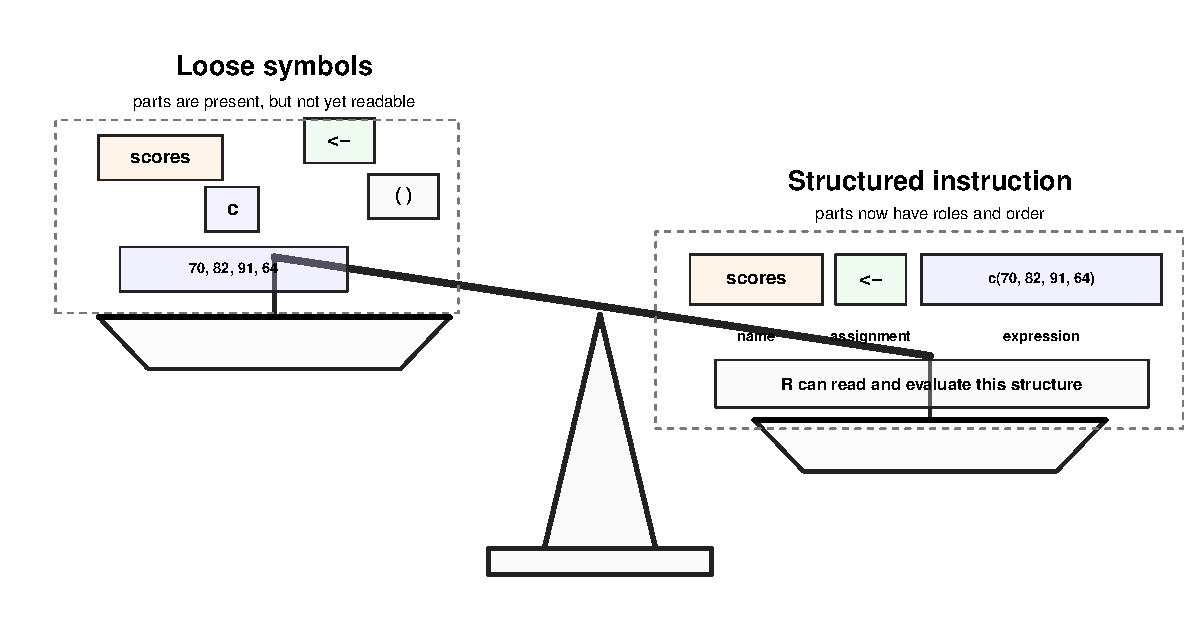
\includegraphics[width=0.9\linewidth,height=\textheight,keepaspectratio]{chapters/06-syntax-as-structure-of-meaning_files/figure-pdf/fig-code-as-structured-instruction-1.pdf}

}

\caption{\label{fig-code-as-structured-instruction}Structured Code
Carries Meaning}

\end{figure}%

As shown in Figure~\ref{fig-code-as-structured-instruction}, the loose
symbols on the left are not useless. They are simply not yet arranged
into a readable instruction. On the right, the same kind of pieces now
have order and roles: \texttt{scores} is the name, \texttt{\textless{}-}
assigns the result, and \texttt{c(70,\ 82,\ 91,\ 64)} creates the values
that will be stored.

The figure is not saying that code becomes correct just because it looks
neat. It is making a smaller point: syntax gives code a structure R can
read. The rest of this chapter explains how that structure works.

\section{R as a Language}\label{r-as-a-language}

R is a programming language, but that phrase can sound distant when a
learner is still trying to understand the Console.

The language comparison is useful, but it has limits. R is not a natural
language like English, Yoruba, French, or Swahili. Natural languages
tolerate context, gesture, ambiguity, and incomplete meaning. R does
not. R is a formal computer language. A broken expression cannot be
rescued by good intentions.

For Leo, the useful point is simple: R understands code because code
follows patterns. A line of R is not a loose collection of marks. It is
an arrangement of values, names, operators, function calls, and storage
instructions.

Mathematical notation gives Leo a familiar clue. The expression
\texttt{10\ +\ 5} is understood because the symbols follow a pattern.
The \texttt{+} sign sits between two values and tells R what operation
to perform.

R also reads through structure and pattern.

When Leo writes:

\begin{Shaded}
\begin{Highlighting}[]
\DecValTok{10} \SpecialCharTok{+} \DecValTok{5}
\CommentTok{\#\textgreater{} [1] 15}
\end{Highlighting}
\end{Shaded}

R does not see disconnected symbols. It sees a valid expression. It
knows that \texttt{+} is being used to add two values.

When Leo writes:

\begin{Shaded}
\begin{Highlighting}[]
\NormalTok{result }\OtherTok{\textless{}{-}} \DecValTok{10} \SpecialCharTok{+} \DecValTok{5}
\end{Highlighting}
\end{Shaded}

R sees an assignment. It evaluates the expression on the right side,
then stores the result in the name on the left side.

Each part has a role in the structure.

\texttt{10} is a value.

\texttt{+} is an operator.

\texttt{10\ +\ 5} is an expression.

\texttt{\textless{}-} performs assignment.

\texttt{result} is a name Leo can use again.

\begin{tcolorbox}[enhanced jigsaw, arc=.35mm, bottomrule=.15mm, breakable, colback=white, colframe=quarto-callout-tip-color-frame, left=2mm, leftrule=.75mm, opacityback=0, rightrule=.15mm, toprule=.15mm]
\begin{minipage}[t]{5.5mm}
\textcolor{quarto-callout-tip-color}{\faLightbulb}
\end{minipage}%
\begin{minipage}[t]{\textwidth - 5.5mm}

\vspace{-3mm}\textbf{Mental Model}\vspace{3mm}

R code is structured meaning.

Leo does not need to memorise every command before he can begin reading
code. He first needs to see the structure that tells R how to read,
evaluate, store, and connect each part.

\end{minipage}%
\end{tcolorbox}

R does not guess what Leo meant. It evaluates what Leo wrote. That is
why syntax matters.

Leo is not merely learning symbols. He is learning how R reads.

\section{What Is an Expression?}\label{what-is-an-expression}

Many R instructions contain expressions. An expression is a piece of R
code that R can evaluate to produce a value.

Evaluation means that R reads the expression, works out its value, and
returns a result.

This definition is short, but it carries a lot of weight. Leo should not
ask first whether a line looks familiar or whether he can translate it
into ordinary words. The first question is more precise:

\begin{Shaded}
\begin{Highlighting}[]
\NormalTok{Can R evaluate this?}
\end{Highlighting}
\end{Shaded}

If R can evaluate it and return a value, Leo is looking at an
expression.

The simplest expression can be a single value:

\begin{Shaded}
\begin{Highlighting}[]
\DecValTok{10}
\CommentTok{\#\textgreater{} [1] 10}
\end{Highlighting}
\end{Shaded}

R evaluates the expression and returns the value \texttt{10}.

Because the expression is not assigned, R also prints the result in the
Console.

A slightly richer expression can be a calculation:

\begin{Shaded}
\begin{Highlighting}[]
\DecValTok{10} \SpecialCharTok{+} \DecValTok{5}
\CommentTok{\#\textgreater{} [1] 15}
\end{Highlighting}
\end{Shaded}

R evaluates the expression and returns the result.

Because the result is not assigned to a name, R prints it immediately in
the Console.

A function call can also be an expression:

\begin{Shaded}
\begin{Highlighting}[]
\FunctionTok{mean}\NormalTok{(}\FunctionTok{c}\NormalTok{(}\DecValTok{70}\NormalTok{, }\DecValTok{82}\NormalTok{, }\DecValTok{91}\NormalTok{, }\DecValTok{64}\NormalTok{))}
\CommentTok{\#\textgreater{} [1] 76.75}
\end{Highlighting}
\end{Shaded}

This line may look more complex, but the idea is the same. R evaluates
the code and returns a value.

The important point is that R code is not only a command shouted at the
computer. Much of R code is made of expressions, and expressions produce
values.

That changes how Leo reads.

Instead of asking only, ``What command is this?'' he begins to ask,
``What value is R trying to produce here?''

That question will help him for the rest of the book.

\section{Expression and Assignment Are Not the Same
Thing}\label{expression-and-assignment-are-not-the-same-thing}

This distinction is small enough to miss and important enough to slow
down for.

An expression produces a value.

An assignment stores a value.

These two lines are related, but they do not do exactly the same thing:

\begin{Shaded}
\begin{Highlighting}[]
\DecValTok{10} \SpecialCharTok{+} \DecValTok{5}
\CommentTok{\#\textgreater{} [1] 15}
\end{Highlighting}
\end{Shaded}

\begin{Shaded}
\begin{Highlighting}[]
\NormalTok{result }\OtherTok{\textless{}{-}} \DecValTok{10} \SpecialCharTok{+} \DecValTok{5}
\end{Highlighting}
\end{Shaded}

In the first line, R evaluates \texttt{10\ +\ 5} and prints the result
because Leo has not asked R to store it.

In the second line, R still evaluates \texttt{10\ +\ 5}, but the
assignment changes what happens next. The result is stored under the
name \texttt{result}.

So the expression is this part:

\begin{Shaded}
\begin{Highlighting}[]
\NormalTok{10 + 5}
\end{Highlighting}
\end{Shaded}

The assignment is the full storage pattern:

\begin{Shaded}
\begin{Highlighting}[]
\NormalTok{result \textless{}{-} 10 + 5}
\end{Highlighting}
\end{Shaded}

Leo can think of it this way:

\begin{Shaded}
\begin{Highlighting}[]
\NormalTok{expression: produce a value}
\NormalTok{assignment: store the produced value in a name}
\end{Highlighting}
\end{Shaded}

This difference explains why some code prints immediately and some code
quietly saves a result for later.

It also protects Leo from a common misunderstanding. Assignment is not
calculation by itself. Assignment is what happens after evaluation, when
R gives the result a name.

\section{Every Expression Returns
Something}\label{every-expression-returns-something}

Leo types a simple expression:

\begin{Shaded}
\begin{Highlighting}[]
\DecValTok{10} \SpecialCharTok{+} \DecValTok{5}
\CommentTok{\#\textgreater{} [1] 15}
\end{Highlighting}
\end{Shaded}

R prints the result because there is no assignment.

Then he types another expression:

\begin{Shaded}
\begin{Highlighting}[]
\FunctionTok{mean}\NormalTok{(}\FunctionTok{c}\NormalTok{(}\DecValTok{70}\NormalTok{, }\DecValTok{82}\NormalTok{, }\DecValTok{91}\NormalTok{, }\DecValTok{64}\NormalTok{))}
\CommentTok{\#\textgreater{} [1] 76.75}
\end{Highlighting}
\end{Shaded}

Again, R prints the result.

Now Leo writes:

\begin{Shaded}
\begin{Highlighting}[]
\NormalTok{score\_mean }\OtherTok{\textless{}{-}} \FunctionTok{mean}\NormalTok{(}\FunctionTok{c}\NormalTok{(}\DecValTok{70}\NormalTok{, }\DecValTok{82}\NormalTok{, }\DecValTok{91}\NormalTok{, }\DecValTok{64}\NormalTok{))}
\end{Highlighting}
\end{Shaded}

This time, nothing appears immediately.

For many beginners, this moment is confusing. The code ran, but the
screen seems quiet.

But the result did not disappear. R evaluated the expression on the
right and stored the answer under the name \texttt{score\_mean}.

Leo can ask for it by typing the name:

\begin{Shaded}
\begin{Highlighting}[]
\NormalTok{score\_mean}
\CommentTok{\#\textgreater{} [1] 76.75}
\end{Highlighting}
\end{Shaded}

\begin{tcolorbox}[enhanced jigsaw, arc=.35mm, bottomrule=.15mm, breakable, colback=white, colframe=quarto-callout-important-color-frame, left=2mm, leftrule=.75mm, opacityback=0, rightrule=.15mm, toprule=.15mm]
\begin{minipage}[t]{5.5mm}
\textcolor{quarto-callout-important-color}{\faExclamation}
\end{minipage}%
\begin{minipage}[t]{\textwidth - 5.5mm}

\vspace{-3mm}\textbf{Reliable Analysis Rule}\vspace{3mm}

If an expression is not assigned, R usually prints the result. If it is
assigned, R stores the result.

Quiet code is not always inactive code. Sometimes R has done the work
and saved the answer for later.

\end{minipage}%
\end{tcolorbox}

This helps Leo understand why R sometimes prints and sometimes stays
silent. R is not being inconsistent. The syntax has changed.

\section{Assignment: Giving a Result a
Name}\label{assignment-giving-a-result-a-name}

Assignment is one of the most important structures in R.

Leo writes:

\begin{Shaded}
\begin{Highlighting}[]
\NormalTok{result }\OtherTok{\textless{}{-}} \DecValTok{10}
\end{Highlighting}
\end{Shaded}

This means:

\begin{Shaded}
\begin{Highlighting}[]
\NormalTok{take the value 10 and store it under the name result}
\end{Highlighting}
\end{Shaded}

The arrow points toward the name that R will use for the result.

The name is not the data itself. The name points to the stored result.
This matters because Leo will soon work with objects much larger than
one number.

For example:

\begin{Shaded}
\begin{Highlighting}[]
\NormalTok{scores }\OtherTok{\textless{}{-}} \FunctionTok{c}\NormalTok{(}\DecValTok{70}\NormalTok{, }\DecValTok{82}\NormalTok{, }\DecValTok{91}\NormalTok{, }\DecValTok{64}\NormalTok{)}
\end{Highlighting}
\end{Shaded}

Here, R evaluates the right side first. The expression
\texttt{c(70,\ 82,\ 91,\ 64)} creates a vector. Then R stores that
vector under the name \texttt{scores}.

Later, Leo can use the name instead of rewriting the whole vector:

\begin{Shaded}
\begin{Highlighting}[]
\NormalTok{avg\_score }\OtherTok{\textless{}{-}} \FunctionTok{mean}\NormalTok{(scores)}
\end{Highlighting}
\end{Shaded}

The assignment pattern is stable:

\begin{Shaded}
\begin{Highlighting}[]
\NormalTok{name \textless{}{-} expression}
\end{Highlighting}
\end{Shaded}

Leo can read it like this:

\begin{Shaded}
\begin{Highlighting}[]
\NormalTok{store the evaluated result of expression inside name}
\end{Highlighting}
\end{Shaded}

That sentence is worth keeping close. It stops assignment from looking
like a strange arrow and turns it into a readable structure.

\texttt{avg\_score\ \textless{}-\ mean(scores)} means R should evaluate
\texttt{mean(scores)} and store the result using the name
\texttt{avg\_score}.

The arrow is not decoration. It is direction.

\section{A Simple Line of R}\label{a-simple-line-of-r}

Leo now returns to a small block of code:

\begin{Shaded}
\begin{Highlighting}[]
\NormalTok{scores }\OtherTok{\textless{}{-}} \FunctionTok{c}\NormalTok{(}\DecValTok{70}\NormalTok{, }\DecValTok{82}\NormalTok{, }\DecValTok{91}\NormalTok{, }\DecValTok{64}\NormalTok{)}
\NormalTok{avg\_score }\OtherTok{\textless{}{-}} \FunctionTok{mean}\NormalTok{(scores)}
\NormalTok{avg\_score}
\CommentTok{\#\textgreater{} [1] 76.75}
\end{Highlighting}
\end{Shaded}

The second line is the one that matters most here:

\begin{Shaded}
\begin{Highlighting}[]
\NormalTok{avg\_score }\OtherTok{\textless{}{-}} \FunctionTok{mean}\NormalTok{(scores)}
\end{Highlighting}
\end{Shaded}

Leo can read it as a plain instruction:

\begin{Shaded}
\begin{Highlighting}[]
\NormalTok{Put the mean of scores into avg\_score.}
\end{Highlighting}
\end{Shaded}

Or more carefully:

\begin{itemize}
\tightlist
\item
  \texttt{scores} is the input object;
\item
  \texttt{mean()} is the action;
\item
  \texttt{mean(scores)} is the expression to evaluate;
\item
  \texttt{\textless{}-} stores the result;
\item
  \texttt{avg\_score} is the name that receives the result.
\end{itemize}

The pattern helps him see roles without pretending that every line of
code must be translated word for word.

A useful beginner reading pattern is:

\begin{Shaded}
\begin{Highlighting}[]
\NormalTok{name \textless{}{-} action(input)}
\end{Highlighting}
\end{Shaded}

In this case:

\begin{Shaded}
\begin{Highlighting}[]
\NormalTok{avg\_score \textless{}{-} mean(scores)}
\end{Highlighting}
\end{Shaded}

means:

\begin{Shaded}
\begin{Highlighting}[]
\NormalTok{store the result of applying mean() to scores inside avg\_score}
\end{Highlighting}
\end{Shaded}

R is strict, but it is not random.

Leo is no longer staring at symbols. He is reading a structured line.

\section{Operators Need Complete
Expressions}\label{operators-need-complete-expressions}

Operators also depend on structure.

This expression works because the \texttt{+} operator has a value on
both sides:

\begin{Shaded}
\begin{Highlighting}[]
\NormalTok{score }\OtherTok{\textless{}{-}} \DecValTok{82}
\NormalTok{score }\SpecialCharTok{+} \DecValTok{5}
\CommentTok{\#\textgreater{} [1] 87}
\end{Highlighting}
\end{Shaded}

This does not form a complete expression:

\begin{Shaded}
\begin{Highlighting}[]
\NormalTok{score }\SpecialCharTok{+}
\CommentTok{\# Error: unexpected end of input}
\end{Highlighting}
\end{Shaded}

The problem is not that \texttt{score} is wrong. The problem is that the
operator is waiting for the other side of the expression.

The same idea will matter in Chapter 7. A comparison such as this also
has structure:

\begin{Shaded}
\begin{Highlighting}[]
\NormalTok{score }\SpecialCharTok{\textgreater{}} \DecValTok{80}
\CommentTok{\#\textgreater{} [1] TRUE}
\end{Highlighting}
\end{Shaded}

There is a name, an operator, and a value. This line asks R to make a
judgment. Chapter 7 will teach that kind of judgment properly. For now,
the syntax lesson is enough: an operator usually needs complete material
around it.

\section{Function Calls as Structured
Expressions}\label{function-calls-as-structured-expressions}

A function call has a recognizable structure:

\begin{Shaded}
\begin{Highlighting}[]
\NormalTok{function\_name(argument)}
\end{Highlighting}
\end{Shaded}

The function name tells R what action to use. The parentheses create the
call. The argument supplies the input.

For example:

\begin{Shaded}
\begin{Highlighting}[]
\FunctionTok{mean}\NormalTok{(scores)}
\CommentTok{\#\textgreater{} [1] 76.75}
\end{Highlighting}
\end{Shaded}

Here, \texttt{mean} is the function name. The object \texttt{scores} is
the argument. The whole expression asks R to calculate the mean of the
values stored in \texttt{scores}.

Another example:

\begin{Shaded}
\begin{Highlighting}[]
\FunctionTok{round}\NormalTok{(}\FloatTok{82.567}\NormalTok{, }\DecValTok{2}\NormalTok{)}
\CommentTok{\#\textgreater{} [1] 82.57}
\end{Highlighting}
\end{Shaded}

Here:

\begin{itemize}
\tightlist
\item
  \texttt{round} is the function name;
\item
  \texttt{82.567} is the value to round;
\item
  \texttt{2} tells R how many decimal places to keep.
\end{itemize}

The comma separates arguments. It tells R that the function is receiving
more than one piece of information.

This structure matters because R is strict. It does not understand
intentions that are not expressed through correct syntax.

This works:

\begin{Shaded}
\begin{Highlighting}[]
\FunctionTok{mean}\NormalTok{(scores)}
\CommentTok{\#\textgreater{} [1] 76.75}
\end{Highlighting}
\end{Shaded}

This does not work:

\begin{Shaded}
\begin{Highlighting}[]
\NormalTok{mean scores}
\CommentTok{\#\textgreater{} Error in parse(text = input): \textless{}text\textgreater{}:1:6: unexpected symbol}
\CommentTok{\#\textgreater{} 1: mean scores}
\CommentTok{\#\textgreater{}          \^{}}
\end{Highlighting}
\end{Shaded}

A human may understand the intention: ``calculate the mean of scores.''

R evaluates the structure that Leo writes.

The missing parentheses change the meaning completely. Without them, R
does not see a proper function call.

Leo learns a practical rule:

\begin{Shaded}
\begin{Highlighting}[]
\NormalTok{A function needs its call structure.}
\end{Highlighting}
\end{Shaded}

In R, that usually means a function name followed by parentheses.

\section{Parentheses Are Not
Decoration}\label{parentheses-are-not-decoration}

Many beginners see parentheses as punctuation. In R, parentheses often
define where an action begins and ends.

Compare this:

\begin{Shaded}
\begin{Highlighting}[]
\FunctionTok{mean}\NormalTok{(scores)}
\CommentTok{\#\textgreater{} [1] 76.75}
\end{Highlighting}
\end{Shaded}

with this:

\begin{Shaded}
\begin{Highlighting}[]
\NormalTok{mean}
\end{Highlighting}
\end{Shaded}

The first line calls the function. It tells R to use \texttt{mean()} on
the object \texttt{scores}.

The second line refers to the function object itself. It does not supply
input. It does not ask R to calculate the mean of anything.

For a beginner, this distinction can be surprising. Leo expected
\texttt{mean} to do something by itself.

R disagrees.

R needs the call structure:

\begin{Shaded}
\begin{Highlighting}[]
\NormalTok{mean(scores)}
\end{Highlighting}
\end{Shaded}

That structure says:

\begin{Shaded}
\begin{Highlighting}[]
\NormalTok{use the function named mean on the object named scores}
\end{Highlighting}
\end{Shaded}

The parentheses complete the function call structure.

Without them, Leo may be pointing at a tool. With them, he is using the
tool.

\section{Evaluation: How R Works Through
Code}\label{evaluation-how-r-works-through-code}

Leo now wants to understand what R is doing behind the screen.

When he writes:

\begin{Shaded}
\begin{Highlighting}[]
\NormalTok{scores }\OtherTok{\textless{}{-}} \FunctionTok{c}\NormalTok{(}\DecValTok{70}\NormalTok{, }\DecValTok{82}\NormalTok{, }\DecValTok{91}\NormalTok{, }\DecValTok{64}\NormalTok{)}
\end{Highlighting}
\end{Shaded}

R does not begin by storing an empty name. It begins by evaluating the
right side.

First, R sees:

\begin{Shaded}
\begin{Highlighting}[]
\FunctionTok{c}\NormalTok{(}\DecValTok{70}\NormalTok{, }\DecValTok{82}\NormalTok{, }\DecValTok{91}\NormalTok{, }\DecValTok{64}\NormalTok{)}
\CommentTok{\#\textgreater{} [1] 70 82 91 64}
\end{Highlighting}
\end{Shaded}

That expression creates a vector.

Then R stores the vector under the name \texttt{scores}.

Now, when Leo writes:

\begin{Shaded}
\begin{Highlighting}[]
\FunctionTok{mean}\NormalTok{(scores)}
\CommentTok{\#\textgreater{} [1] 76.75}
\end{Highlighting}
\end{Shaded}

R looks for an object named \texttt{scores}. If it finds that object, it
passes the values into \texttt{mean()} and returns the result.

This is why some errors become easier to understand when Leo thinks in
terms of evaluation.

For example:

\begin{Shaded}
\begin{Highlighting}[]
\FunctionTok{mean}\NormalTok{(missing\_score)}
\CommentTok{\#\textgreater{} Error: object \textquotesingle{}missing\_score\textquotesingle{} not found}
\end{Highlighting}
\end{Shaded}

The syntax of the function call is fine. There is a function name,
parentheses, and an argument.

The problem is different.

No object named \texttt{missing\_score} has been created.

So R looks for \texttt{missing\_score} and cannot find it.

That is not a statistics problem. It is a naming problem.

Not every error means Leo has misunderstood the analysis. Sometimes R is
simply saying, ``I cannot find the object you named.''

Learning syntax helps Leo separate those problems.

He can ask:

\begin{itemize}
\tightlist
\item
  Is the structure valid?
\item
  Does the object exist?
\item
  Is the name spelled exactly the same way?
\item
  Did I assign the result before trying to use it?
\end{itemize}

These questions do more than fix errors. They build confidence.

\section{The Inside-Out Rule}\label{the-inside-out-rule}

Now Leo meets a line that looks more crowded:

\begin{Shaded}
\begin{Highlighting}[]
\FunctionTok{round}\NormalTok{(}\FunctionTok{mean}\NormalTok{(}\FunctionTok{c}\NormalTok{(}\DecValTok{70}\NormalTok{, }\DecValTok{82}\NormalTok{, }\DecValTok{91}\NormalTok{, }\DecValTok{64}\NormalTok{)), }\DecValTok{2}\NormalTok{)}
\CommentTok{\#\textgreater{} [1] 76.75}
\end{Highlighting}
\end{Shaded}

At first, the line seems to ask for too much at once. But it follows a
simple rule:

\begin{tcolorbox}[enhanced jigsaw, arc=.35mm, bottomrule=.15mm, breakable, colback=white, colframe=quarto-callout-tip-color-frame, left=2mm, leftrule=.75mm, opacityback=0, rightrule=.15mm, toprule=.15mm]
\begin{minipage}[t]{5.5mm}
\textcolor{quarto-callout-tip-color}{\faLightbulb}
\end{minipage}%
\begin{minipage}[t]{\textwidth - 5.5mm}

\vspace{-3mm}\textbf{The Inside-Out Rule}\vspace{3mm}

R evaluates nested expressions from the inside outward.

When one expression sits inside another expression, R works through the
inner expression first, then carries the result outward.

\end{minipage}%
\end{tcolorbox}

The order is:

\begin{enumerate}
\def\labelenumi{\arabic{enumi}.}
\tightlist
\item
  \texttt{c(70,\ 82,\ 91,\ 64)}
\item
  \texttt{mean(...)}
\item
  \texttt{round(...)}
\end{enumerate}

First, R creates the vector:

\begin{Shaded}
\begin{Highlighting}[]
\FunctionTok{c}\NormalTok{(}\DecValTok{70}\NormalTok{, }\DecValTok{82}\NormalTok{, }\DecValTok{91}\NormalTok{, }\DecValTok{64}\NormalTok{)}
\CommentTok{\#\textgreater{} [1] 70 82 91 64}
\end{Highlighting}
\end{Shaded}

Then R calculates the mean:

\begin{Shaded}
\begin{Highlighting}[]
\FunctionTok{mean}\NormalTok{(}\FunctionTok{c}\NormalTok{(}\DecValTok{70}\NormalTok{, }\DecValTok{82}\NormalTok{, }\DecValTok{91}\NormalTok{, }\DecValTok{64}\NormalTok{))}
\CommentTok{\#\textgreater{} [1] 76.75}
\end{Highlighting}
\end{Shaded}

Then R rounds the result:

\begin{Shaded}
\begin{Highlighting}[]
\FunctionTok{round}\NormalTok{(}\FunctionTok{mean}\NormalTok{(}\FunctionTok{c}\NormalTok{(}\DecValTok{70}\NormalTok{, }\DecValTok{82}\NormalTok{, }\DecValTok{91}\NormalTok{, }\DecValTok{64}\NormalTok{)), }\DecValTok{2}\NormalTok{)}
\CommentTok{\#\textgreater{} [1] 76.75}
\end{Highlighting}
\end{Shaded}

Leo can write the same logic in separate lines:

\begin{Shaded}
\begin{Highlighting}[]
\NormalTok{scores }\OtherTok{\textless{}{-}} \FunctionTok{c}\NormalTok{(}\DecValTok{70}\NormalTok{, }\DecValTok{82}\NormalTok{, }\DecValTok{91}\NormalTok{, }\DecValTok{64}\NormalTok{)}
\NormalTok{avg\_score }\OtherTok{\textless{}{-}} \FunctionTok{mean}\NormalTok{(scores)}
\NormalTok{rounded\_avg }\OtherTok{\textless{}{-}} \FunctionTok{round}\NormalTok{(avg\_score, }\DecValTok{2}\NormalTok{)}
\NormalTok{rounded\_avg}
\CommentTok{\#\textgreater{} [1] 76.75}
\end{Highlighting}
\end{Shaded}

Both versions can produce the same result.

The nested version is shorter. The step-by-step version is easier to
inspect.

A professional does not always choose the shortest code. A professional
chooses code that is clear enough to trust.

That sentence matters. Leo is not learning R to impress the Console with
compact lines. He is learning R to produce work that can be read,
checked, repaired, and repeated.

\section{Why Nested Code Confuses
Beginners}\label{why-nested-code-confuses-beginners}

Nested code often confuses beginners because humans and R do not always
read in the same order.

Leo sees this:

\begin{Shaded}
\begin{Highlighting}[]
\FunctionTok{round}\NormalTok{(}\FunctionTok{mean}\NormalTok{(}\FunctionTok{c}\NormalTok{(}\DecValTok{70}\NormalTok{, }\DecValTok{82}\NormalTok{, }\DecValTok{91}\NormalTok{, }\DecValTok{64}\NormalTok{)), }\DecValTok{2}\NormalTok{)}
\CommentTok{\#\textgreater{} [1] 76.75}
\end{Highlighting}
\end{Shaded}

His eyes naturally move from left to right. He sees \texttt{round()}
first because it appears first.

But R must evaluate the innermost part first.

That mismatch creates confusion. Leo's eyes begin outside. R begins
inside.

A helpful practice is to make the layers visible:

\begin{Shaded}
\begin{Highlighting}[]
\NormalTok{round(}
\NormalTok{  mean(}
\NormalTok{    c(70, 82, 91, 64)}
\NormalTok{  ),}
\NormalTok{  2}
\NormalTok{)}
\end{Highlighting}
\end{Shaded}

Now the structure is easier to see.

The innermost expression creates the values:

\begin{Shaded}
\begin{Highlighting}[]
\NormalTok{c(70, 82, 91, 64)}
\end{Highlighting}
\end{Shaded}

The middle expression calculates the mean:

\begin{Shaded}
\begin{Highlighting}[]
\NormalTok{mean(...)}
\end{Highlighting}
\end{Shaded}

The outer expression rounds the final result:

\begin{Shaded}
\begin{Highlighting}[]
\NormalTok{round(..., 2)}
\end{Highlighting}
\end{Shaded}

This does not change what R evaluates. It changes what Leo can see.

Readable formatting is not cosmetic. It is part of understanding.

Code is not only for R. Code must also remain readable to the human who
returns to it later, whether that is Leo, a collaborator, or a future
reviewer.

Clear code is a gift to that future reader.

\section{Common Beginner Mistake: Reading Code as
Magic}\label{common-beginner-mistake-reading-code-as-magic}

\begin{tcolorbox}[enhanced jigsaw, arc=.35mm, bottomrule=.15mm, breakable, colback=white, colframe=quarto-callout-warning-color-frame, left=2mm, leftrule=.75mm, opacityback=0, rightrule=.15mm, toprule=.15mm]
\begin{minipage}[t]{5.5mm}
\textcolor{quarto-callout-warning-color}{\faExclamationTriangle}
\end{minipage}%
\begin{minipage}[t]{\textwidth - 5.5mm}

\vspace{-3mm}\textbf{Common Beginner Trap}\vspace{3mm}

A common beginner mistake is to copy code that works without reading its
grammar.

When the code works, the learner moves on. When the code breaks, there
is no structure to inspect.

\end{minipage}%
\end{tcolorbox}

Consider this line:

\begin{Shaded}
\begin{Highlighting}[]
\FunctionTok{round}\NormalTok{(}\FunctionTok{mean}\NormalTok{(scores), }\DecValTok{2}\NormalTok{)}
\CommentTok{\#\textgreater{} [1] 76.75}
\end{Highlighting}
\end{Shaded}

A beginner may copy it because it works. Leo is learning to do something
better. He is learning to read it.

He can ask:

\begin{itemize}
\tightlist
\item
  What is being evaluated?
\item
  What is being assigned?
\item
  Which object is being used?
\item
  Which function is being called?
\item
  What is inside the parentheses?
\item
  What runs first?
\end{itemize}

The answers turn the line into language.

\texttt{mean(scores)} is evaluated first.

The result of \texttt{mean(scores)} is passed into \texttt{round()}.

The value \texttt{2} tells \texttt{round()} how many decimal places to
keep.

Each part has a role in the evaluation.

This is how Leo begins to move from copying code to understanding code.
He may still copy examples while learning, but he now reads their
structure.

He reads before he runs.

\section{Try It Yourself}\label{try-it-yourself}

Create a vector of project scores:

\begin{Shaded}
\begin{Highlighting}[]
\NormalTok{project\_scores }\OtherTok{\textless{}{-}} \FunctionTok{c}\NormalTok{(}\DecValTok{72}\NormalTok{, }\DecValTok{85}\NormalTok{, }\DecValTok{90}\NormalTok{, }\DecValTok{68}\NormalTok{, }\DecValTok{77}\NormalTok{)}
\end{Highlighting}
\end{Shaded}

Now calculate the mean:

\begin{Shaded}
\begin{Highlighting}[]
\FunctionTok{mean}\NormalTok{(project\_scores)}
\CommentTok{\#\textgreater{} [1] 78.4}
\end{Highlighting}
\end{Shaded}

Before running the next line, predict which part R evaluates first.

Then round the mean to one decimal place:

\begin{Shaded}
\begin{Highlighting}[]
\FunctionTok{round}\NormalTok{(}\FunctionTok{mean}\NormalTok{(project\_scores), }\DecValTok{1}\NormalTok{)}
\CommentTok{\#\textgreater{} [1] 78.4}
\end{Highlighting}
\end{Shaded}

Now rewrite the nested version as separate steps:

\begin{Shaded}
\begin{Highlighting}[]
\NormalTok{project\_scores }\OtherTok{\textless{}{-}} \FunctionTok{c}\NormalTok{(}\DecValTok{72}\NormalTok{, }\DecValTok{85}\NormalTok{, }\DecValTok{90}\NormalTok{, }\DecValTok{68}\NormalTok{, }\DecValTok{77}\NormalTok{)}
\NormalTok{avg\_project\_score }\OtherTok{\textless{}{-}} \FunctionTok{mean}\NormalTok{(project\_scores)}
\NormalTok{rounded\_project\_score }\OtherTok{\textless{}{-}} \FunctionTok{round}\NormalTok{(avg\_project\_score, }\DecValTok{1}\NormalTok{)}
\NormalTok{rounded\_project\_score}
\CommentTok{\#\textgreater{} [1] 78.4}
\end{Highlighting}
\end{Shaded}

Pause before moving on.

Which version is easier to read?

Which version is shorter?

Which version makes the order of work most visible?

There is no single answer for all situations. The point is to notice
structure. Sometimes compact code is clear. Sometimes step-by-step code
is safer. Leo's task is to understand the grammar beneath both.

\section{Short Recap}\label{short-recap}

Leo began this chapter seeing code as a possible pile of symbols. He now
sees structure.

Syntax arranges names, values, operators, functions, and punctuation so
R can evaluate an instruction. Expressions produce values. Assignment
stores evaluated results. Error messages often point to where the
structure breaks.

The central idea is simple:

\begin{Shaded}
\begin{Highlighting}[]
\NormalTok{R evaluates expressions, and syntax tells R how those expressions are structured.}
\end{Highlighting}
\end{Shaded}

Syntax is not punctuation. Syntax is meaning arranged so R can evaluate
it.

\section{Leo's Notebook}\label{leos-notebook-2}

Leo writes:

\begin{quote}
I used to see R code as symbols I had to memorise. Now I see that each
line has a structure. If I can find the expression, the assignment, the
function call, and the input, I can read the line before I panic.
\end{quote}

He pauses, then adds one more note:

\begin{quote}
Nested code is not harder because R is mysterious. It is harder because
my eyes read from the outside, while R evaluates from the inside. When
the line becomes crowded, I can rewrite it as clearer steps.
\end{quote}

That insight will save him many hours later.

When a line becomes confusing, Leo does not need to panic. He can slow
it down. He can find the innermost expression. He can name the result.
He can rewrite the line as steps.

This is not weakness. This is how careful analysts work.

\section{Glossary}\label{glossary}

\textbf{Syntax}\\
The rules that define how R code must be written so R can understand and
evaluate it.

\textbf{Expression}\\
A piece of code that R can evaluate to produce a value.

\textbf{Evaluation}\\
The process by which R reads an expression, works out its value, and
returns a result.

\textbf{Assignment}\\
The act of storing the evaluated result of an expression in a named
object.

\textbf{Operator}\\
A symbol that tells R to perform an operation on one or more values.

\textbf{Function call}\\
The use of a function name with parentheses and arguments to perform an
action.

\textbf{Argument}\\
An input supplied to a function.

\textbf{Nested expression}\\
An expression placed inside another expression.

\textbf{Inside-out rule}\\
The principle that R evaluates inner expressions before outer
expressions.

\section{Chapter Outcome}\label{chapter-outcome-5}

By the end of this chapter, Leo can:

\begin{itemize}
\tightlist
\item
  describe R as a language with syntax;
\item
  identify simple expressions;
\item
  explain that expressions return values;
\item
  distinguish an expression from an assignment;
\item
  explain how assignment stores evaluated results;
\item
  read simple function calls;
\item
  understand why parentheses matter;
\item
  trace nested execution from the inside outward;
\item
  rewrite nested expressions into clearer step-by-step code;
\item
  explain why readable code is part of reliable analysis.
\end{itemize}

\section{Transition to Chapter 7}\label{transition-to-chapter-7}

Leo now knows that R code has grammar.

He can see the shape of a line. He can identify an expression. He can
understand assignment. He can read a function call. He can slow down
nested code and trace how R works from the inside outward.

But grammar alone is not enough.

A sentence can be well formed and still need a decision. A research
dataset can be neatly structured and still require judgment: Which
values count? Which rows qualify? Which learners completed the task?
Which scores are above the threshold? Which cases should be kept,
compared, or filtered?

That is where logic enters.

In the next chapter, Leo will meet the decision-making side of R. He
will learn how \texttt{TRUE} and \texttt{FALSE} help R represent answers
to questions. He will see how arithmetic operators calculate, how
comparison operators test relationships, and how logical operators
combine conditions. He will also learn why \texttt{\textless{}-},
\texttt{=}, and \texttt{==} do not mean the same thing, even though they
look close enough to confuse almost every beginner at least once.

Chapter 6 has shown Leo how R reads structured meaning.

Chapter 7 will show him how R begins to judge.

\chapter{Logic in R: How Code Makes
Judgments}\label{logic-in-r-how-code-makes-judgments}

\renewcommand{\thefigure}{7.\arabic{figure}}
\setcounter{figure}{0}
\renewcommand{\thetable}{7.\arabic{table}}
\setcounter{table}{0}

\section{Opening Scene: When Code Has to
Decide}\label{opening-scene-when-code-has-to-decide}

Leo can now read a simple line of R as structured code.

He knows that values can be stored under names. He knows that structures
hold values together. He knows that syntax gives code a readable shape.

Then he writes this:

\begin{Shaded}
\begin{Highlighting}[]
\NormalTok{study\_hours }\OtherTok{\textless{}{-}} \DecValTok{6}
\NormalTok{study\_hours }\SpecialCharTok{\textgreater{}} \DecValTok{5}
\CommentTok{\#\textgreater{} [1] TRUE}
\end{Highlighting}
\end{Shaded}

The result is not another number.

It is a judgment:

\begin{Shaded}
\begin{Highlighting}[]
\ConstantTok{TRUE}
\CommentTok{\#\textgreater{} [1] TRUE}
\end{Highlighting}
\end{Shaded}

Something has changed. R is no longer only calculating a value or
storing an object. It is evaluating a condition.

That small judgment sits behind serious data work. Filtering rows,
checking missing values, identifying learners who meet a rule, and
deciding whether code should run all depend on logical thinking.

A researcher may ask:

\begin{itemize}
\tightlist
\item
  Which learners studied more than five hours?
\item
  Which project scores are at least 80?
\item
  Which rows contain missing values?
\item
  Which learners completed their first script?
\item
  Which observations should be kept, removed, grouped, or inspected?
\end{itemize}

R cannot answer these questions by guessing. It needs expressions that
turn questions into conditions.

\begin{tcolorbox}[enhanced jigsaw, arc=.35mm, bottomrule=.15mm, breakable, colback=white, colframe=quarto-callout-note-color-frame, left=2mm, leftrule=.75mm, opacityback=0, rightrule=.15mm, toprule=.15mm]
\begin{minipage}[t]{5.5mm}
\textcolor{quarto-callout-note-color}{\faInfo}
\end{minipage}%
\begin{minipage}[t]{\textwidth - 5.5mm}

\vspace{-3mm}\textbf{Chapter Compass}\vspace{3mm}

This chapter teaches logic as R's system of judgment. By the end, Leo
should be able to:

\begin{itemize}
\tightlist
\item
  recognise logical values such as \texttt{TRUE} and \texttt{FALSE};
\item
  use comparison operators to ask questions;
\item
  use logical operators to combine or reverse judgments;
\item
  distinguish assignment from comparison;
\item
  explain why \texttt{\&} differs from \texttt{\&\&}, and why
  \texttt{\textbar{}} differs from \texttt{\textbar{}\textbar{}};
\item
  understand why \texttt{if} needs one logical answer;
\item
  see how vectorised logic produces many answers;
\item
  use \texttt{is.na()} to check missing values;
\item
  treat wider operator families as preview material rather than a
  memorisation list.
\end{itemize}

\end{minipage}%
\end{tcolorbox}

\section{What Changed After Chapter
6}\label{what-changed-after-chapter-6}

Chapter 6 showed that code needs structure. A line of R is not a pile of
symbols. Names, values, operators, function calls, commas, and
parentheses must be arranged so R can read them.

Chapter 7 moves from structure into judgment.

The new question is not only:

\begin{quote}
Can R read this expression?
\end{quote}

It is also:

\begin{quote}
What judgment does this expression produce?
\end{quote}

\begin{tcolorbox}[enhanced jigsaw, arc=.35mm, bottomrule=.15mm, breakable, colback=white, colframe=quarto-callout-tip-color-frame, left=2mm, leftrule=.75mm, opacityback=0, rightrule=.15mm, toprule=.15mm]
\begin{minipage}[t]{5.5mm}
\textcolor{quarto-callout-tip-color}{\faLightbulb}
\end{minipage}%
\begin{minipage}[t]{\textwidth - 5.5mm}

\vspace{-3mm}\textbf{Core Mental Model}\vspace{3mm}

Syntax tells R how to read an expression.

Logic tells R how to judge a condition.

\end{minipage}%
\end{tcolorbox}

A calculation asks, ``What value should be produced?''

A logical test asks, ``Is this condition true?''

That difference matters because data work constantly asks R to decide
what qualifies.

\section{\texorpdfstring{Logical Values: \texttt{TRUE} and
\texttt{FALSE}}{Logical Values: TRUE and FALSE}}\label{logical-values-true-and-false}

R has two central logical values:

\begin{Shaded}
\begin{Highlighting}[]
\ConstantTok{TRUE}
\CommentTok{\#\textgreater{} [1] TRUE}
\ConstantTok{FALSE}
\CommentTok{\#\textgreater{} [1] FALSE}
\end{Highlighting}
\end{Shaded}

They are not text. They are not written inside quotation marks.

Compare:

\begin{Shaded}
\begin{Highlighting}[]
\FunctionTok{class}\NormalTok{(}\ConstantTok{TRUE}\NormalTok{)}
\CommentTok{\#\textgreater{} [1] "logical"}
\FunctionTok{class}\NormalTok{(}\StringTok{"TRUE"}\NormalTok{)}
\CommentTok{\#\textgreater{} [1] "character"}
\end{Highlighting}
\end{Shaded}

\texttt{TRUE} is a logical value. \texttt{"TRUE"} is character text.

That distinction matters because logical values can guide decisions.
They can be stored, counted, reversed, combined, and used to select
data.

Try a small condition:

\begin{Shaded}
\begin{Highlighting}[]
\DecValTok{10} \SpecialCharTok{\textgreater{}} \DecValTok{5}
\CommentTok{\#\textgreater{} [1] TRUE}
\DecValTok{10} \SpecialCharTok{\textless{}} \DecValTok{5}
\CommentTok{\#\textgreater{} [1] FALSE}
\DecValTok{10} \SpecialCharTok{==} \DecValTok{10}
\CommentTok{\#\textgreater{} [1] TRUE}
\end{Highlighting}
\end{Shaded}

Each expression asks a question and returns a logical answer.

The question may involve one value, as above. Later, the same idea can
be applied across many values or many rows.

\begin{tcolorbox}[enhanced jigsaw, arc=.35mm, bottomrule=.15mm, breakable, colback=white, colframe=quarto-callout-important-color-frame, left=2mm, leftrule=.75mm, opacityback=0, rightrule=.15mm, toprule=.15mm]
\begin{minipage}[t]{5.5mm}
\textcolor{quarto-callout-important-color}{\faExclamation}
\end{minipage}%
\begin{minipage}[t]{\textwidth - 5.5mm}

\vspace{-3mm}\textbf{Reliable Analysis Rule}\vspace{3mm}

\texttt{TRUE} and \texttt{FALSE} are real values.

They are the decision values behind filtering, checking, subsetting, and
conditional execution.

\end{minipage}%
\end{tcolorbox}

\section{From Calculation to
Judgment}\label{from-calculation-to-judgment}

Arithmetic operators calculate. Comparison operators judge.

This is a calculation:

\begin{Shaded}
\begin{Highlighting}[]
\DecValTok{10} \SpecialCharTok{+} \DecValTok{5}
\CommentTok{\#\textgreater{} [1] 15}
\end{Highlighting}
\end{Shaded}

This is a judgment:

\begin{Shaded}
\begin{Highlighting}[]
\DecValTok{10} \SpecialCharTok{\textgreater{}} \DecValTok{5}
\CommentTok{\#\textgreater{} [1] TRUE}
\end{Highlighting}
\end{Shaded}

Both use symbols. They do different jobs.

\begin{longtable}[]{@{}
  >{\raggedright\arraybackslash}p{(\linewidth - 4\tabcolsep) * \real{0.3333}}
  >{\raggedright\arraybackslash}p{(\linewidth - 4\tabcolsep) * \real{0.3333}}
  >{\raggedright\arraybackslash}p{(\linewidth - 4\tabcolsep) * \real{0.3333}}@{}}
\caption{Main operator families Leo meets in early R
code}\label{tbl-operator-families}\tabularnewline
\toprule\noalign{}
\begin{minipage}[b]{\linewidth}\raggedright
Operator family
\end{minipage} & \begin{minipage}[b]{\linewidth}\raggedright
Main job
\end{minipage} & \begin{minipage}[b]{\linewidth}\raggedright
Examples
\end{minipage} \\
\midrule\noalign{}
\endfirsthead
\toprule\noalign{}
\begin{minipage}[b]{\linewidth}\raggedright
Operator family
\end{minipage} & \begin{minipage}[b]{\linewidth}\raggedright
Main job
\end{minipage} & \begin{minipage}[b]{\linewidth}\raggedright
Examples
\end{minipage} \\
\midrule\noalign{}
\endhead
\bottomrule\noalign{}
\endlastfoot
Arithmetic & calculate numeric results & \texttt{+}, \texttt{-},
\texttt{*}, \texttt{/}, \texttt{\^{}}, \texttt{\%\%}, \texttt{\%/\%} \\
Comparison & compare values and return logical results &
\texttt{\textgreater{}}, \texttt{\textless{}}, \texttt{\textgreater{}=},
\texttt{\textless{}=}, \texttt{==}, \texttt{!=} \\
Logical & combine or reverse logical results & \texttt{\&},
\texttt{\&\&}, \texttt{\textbackslash{}\textbar{}},
\texttt{\textbackslash{}\textbar{}\textbackslash{}\textbar{}},
\texttt{!} \\
Assignment & store values in names & \texttt{\textless{}-}, \texttt{=},
\texttt{-\textgreater{}} \\
Subsetting and access & select or access parts of objects &
\texttt{{[}\ {]}}, \texttt{{[}{[}\ {]}{]}}, \texttt{\$} \\
\end{longtable}

This map is deliberately small. Leo will meet other operator families
later, but these are the ones that matter most for the logic chapter.

\section{Comparison Operators: Asking
Questions}\label{comparison-operators-asking-questions}

Comparison operators ask whether a relationship is true.

\begin{longtable}[]{@{}lll@{}}
\caption{Common comparison operators and their
meaning}\label{tbl-comparison-operators}\tabularnewline
\toprule\noalign{}
Operator & Meaning & Example \\
\midrule\noalign{}
\endfirsthead
\toprule\noalign{}
Operator & Meaning & Example \\
\midrule\noalign{}
\endhead
\bottomrule\noalign{}
\endlastfoot
\texttt{\textgreater{}} & greater than &
\texttt{score\ \textgreater{}\ 80} \\
\texttt{\textless{}} & less than & \texttt{score\ \textless{}\ 80} \\
\texttt{\textgreater{}=} & greater than or equal to &
\texttt{score\ \textgreater{}=\ 80} \\
\texttt{\textless{}=} & less than or equal to &
\texttt{score\ \textless{}=\ 80} \\
\texttt{==} & exactly equal to & \texttt{score\ ==\ 80} \\
\texttt{!=} & not equal to & \texttt{score\ !=\ 80} \\
\end{longtable}

Use a small learner score:

\begin{Shaded}
\begin{Highlighting}[]
\NormalTok{score }\OtherTok{\textless{}{-}} \DecValTok{82}
\NormalTok{score }\SpecialCharTok{\textgreater{}} \DecValTok{80}
\CommentTok{\#\textgreater{} [1] TRUE}
\NormalTok{score }\SpecialCharTok{==} \DecValTok{82}
\CommentTok{\#\textgreater{} [1] TRUE}
\NormalTok{score }\SpecialCharTok{!=} \DecValTok{70}
\CommentTok{\#\textgreater{} [1] TRUE}
\end{Highlighting}
\end{Shaded}

The first line stores a value. The remaining lines ask questions about
that value.

A comparison is not just a symbol between two values. It is a question
written in a form R can evaluate.

When R evaluates a condition, the result is a logical judgment.
Sometimes the judgment is one value: \texttt{TRUE} or \texttt{FALSE}.
Sometimes, when the same condition is applied across several values, R
returns several judgments.

The figure below gives a simple map of that idea.

\begin{figure}

\centering{

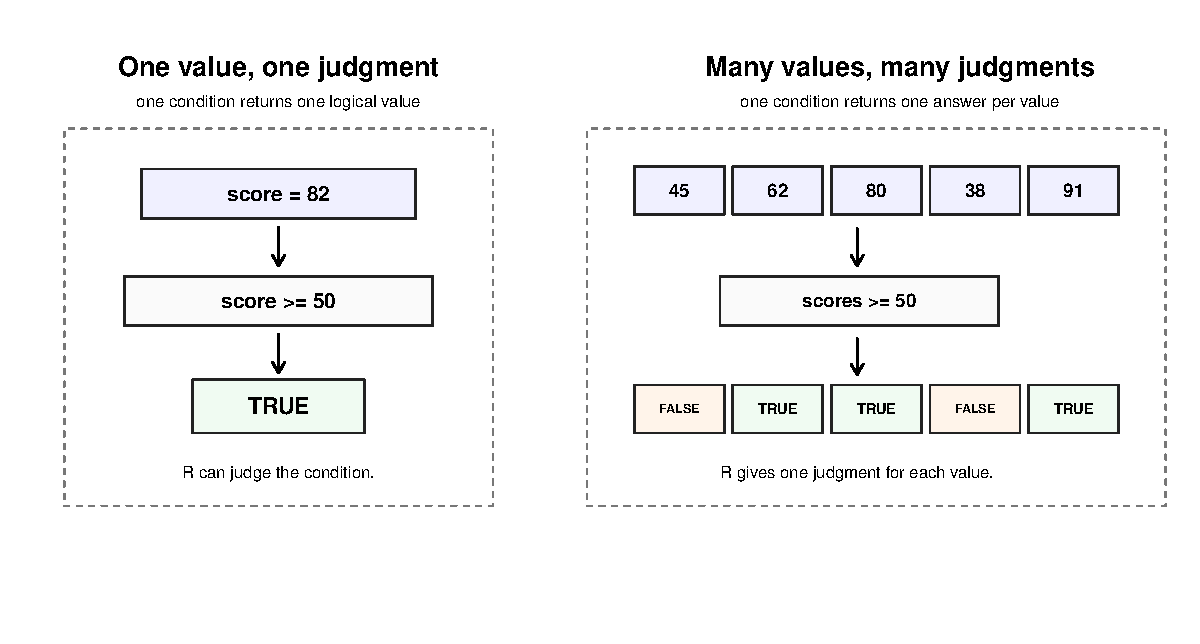
\includegraphics[width=0.9\linewidth,height=\textheight,keepaspectratio]{chapters/07-logic-in-r_files/figure-pdf/fig-condition-to-logical-judgment-1.pdf}

}

\caption{\label{fig-condition-to-logical-judgment}From Conditions to
Logical Judgments}

\end{figure}%

As shown in Figure~\ref{fig-condition-to-logical-judgment}, logic begins
with a condition. In the first panel, one score is tested and R returns
one judgment. In the second panel, the same kind of rule is applied
across several scores, so R returns one judgment for each value.

This is why logical values matter. They are not decorative outputs. They
are the answers R produces when code asks a condition.

\section{Predict Before You Run}\label{predict-before-you-run-2}

Before running the next chunk, pause and predict the output.

Will each expression return \texttt{TRUE} or \texttt{FALSE}?

\begin{Shaded}
\begin{Highlighting}[]
\NormalTok{score }\OtherTok{\textless{}{-}} \DecValTok{82}
\NormalTok{score }\SpecialCharTok{\textgreater{}} \DecValTok{80}
\CommentTok{\#\textgreater{} [1] TRUE}
\NormalTok{score }\SpecialCharTok{==} \DecValTok{80}
\CommentTok{\#\textgreater{} [1] FALSE}
\NormalTok{score }\SpecialCharTok{!=} \DecValTok{70}
\CommentTok{\#\textgreater{} [1] TRUE}
\end{Highlighting}
\end{Shaded}

The point is not speed. The point is to begin reading conditions as
questions.

In plain language:

\begin{itemize}
\tightlist
\item
  \texttt{score\ \textgreater{}\ 80} asks whether the score is greater
  than 80;
\item
  \texttt{score\ ==\ 80} asks whether the score is exactly 80;
\item
  \texttt{score\ !=\ 70} asks whether the score is not 70.
\end{itemize}

Prediction forces Leo to reason before the console answers for him.

\section{Assignment Is Not
Comparison}\label{assignment-is-not-comparison}

One of the most common beginner mistakes is confusing storage with
equality.

These lines do different jobs:

\begin{Shaded}
\begin{Highlighting}[]
\NormalTok{score }\OtherTok{\textless{}{-}} \DecValTok{80}
\NormalTok{score }\SpecialCharTok{==} \DecValTok{80}
\CommentTok{\#\textgreater{} [1] TRUE}
\end{Highlighting}
\end{Shaded}

\texttt{\textless{}-} assigns. It stores \texttt{80} in the name
\texttt{score}.

\texttt{==} compares. It asks whether \texttt{score} is equal to
\texttt{80}.

The equals sign \texttt{=} can assign in some contexts, and it is
commonly used to name function arguments:

\begin{Shaded}
\begin{Highlighting}[]
\FunctionTok{round}\NormalTok{(}\FloatTok{77.46}\NormalTok{, }\AttributeTok{digits =} \DecValTok{1}\NormalTok{)}
\CommentTok{\#\textgreater{} [1] 77.5}
\end{Highlighting}
\end{Shaded}

For clarity in this book, Leo should use:

\begin{itemize}
\tightlist
\item
  \texttt{\textless{}-} for ordinary assignment;
\item
  \texttt{=} mainly for naming function arguments;
\item
  \texttt{==} for equality tests.
\end{itemize}

\begin{tcolorbox}[enhanced jigsaw, arc=.35mm, bottomrule=.15mm, breakable, colback=white, colframe=quarto-callout-warning-color-frame, left=2mm, leftrule=.75mm, opacityback=0, rightrule=.15mm, toprule=.15mm]
\begin{minipage}[t]{5.5mm}
\textcolor{quarto-callout-warning-color}{\faExclamationTriangle}
\end{minipage}%
\begin{minipage}[t]{\textwidth - 5.5mm}

\vspace{-3mm}\textbf{Common Beginner Trap}\vspace{3mm}

Leo wants to test whether \texttt{score} is equal to 80.

He writes:

\begin{Shaded}
\begin{Highlighting}[]
\NormalTok{score }\OtherTok{=} \DecValTok{80}
\end{Highlighting}
\end{Shaded}

That code runs, but it assigns. It does not test equality.

The comparison he wanted is:

\begin{Shaded}
\begin{Highlighting}[]
\NormalTok{score }\SpecialCharTok{==} \DecValTok{80}
\CommentTok{\#\textgreater{} [1] TRUE}
\end{Highlighting}
\end{Shaded}

A single missing \texttt{=} changes the meaning of the line.

\end{minipage}%
\end{tcolorbox}

This is a useful moment of friction. R is not punishing the learner. It
is following the operator that was written.

\section{Logical Operators: Combining
Conditions}\label{logical-operators-combining-conditions}

Comparison operators create judgments. Logical operators combine or
reverse those judgments.

Suppose Leo has two learner indicators:

\begin{Shaded}
\begin{Highlighting}[]
\NormalTok{study\_hours }\OtherTok{\textless{}{-}} \DecValTok{6}
\NormalTok{project\_score }\OtherTok{\textless{}{-}} \DecValTok{85}

\NormalTok{study\_hours }\SpecialCharTok{\textgreater{}} \DecValTok{5}
\CommentTok{\#\textgreater{} [1] TRUE}
\NormalTok{project\_score }\SpecialCharTok{\textgreater{}} \DecValTok{80}
\CommentTok{\#\textgreater{} [1] TRUE}
\end{Highlighting}
\end{Shaded}

The first comparison asks whether study hours are greater than 5. The
second asks whether project score is greater than 80.

Now combine both conditions:

\begin{Shaded}
\begin{Highlighting}[]
\NormalTok{study\_hours }\SpecialCharTok{\textgreater{}} \DecValTok{5} \SpecialCharTok{\&}\NormalTok{ project\_score }\SpecialCharTok{\textgreater{}} \DecValTok{80}
\CommentTok{\#\textgreater{} [1] TRUE}
\end{Highlighting}
\end{Shaded}

This asks whether both conditions are true.

Logical operators do not calculate new measurements. They combine or
reverse logical judgments. They build rules from logical results.

\begin{itemize}
\tightlist
\item
  \texttt{\&} means AND, position by position when there are many
  values.
\item
  \texttt{\textbar{}} means OR, position by position when there are many
  values.
\item
  \texttt{!} reverses a logical value.
\item
  \texttt{\&\&} means AND for a single control decision.
\item
  \texttt{\textbar{}\textbar{}} means OR for a single control decision.
\end{itemize}

Try the basic forms:

\begin{Shaded}
\begin{Highlighting}[]
\NormalTok{study\_hours }\OtherTok{\textless{}{-}} \DecValTok{6}
\NormalTok{project\_score }\OtherTok{\textless{}{-}} \DecValTok{85}
\NormalTok{first\_script\_completed }\OtherTok{\textless{}{-}} \ConstantTok{FALSE}

\NormalTok{study\_hours }\SpecialCharTok{\textgreater{}} \DecValTok{5} \SpecialCharTok{\&}\NormalTok{ project\_score }\SpecialCharTok{\textgreater{}} \DecValTok{80}
\CommentTok{\#\textgreater{} [1] TRUE}
\NormalTok{study\_hours }\SpecialCharTok{\textgreater{}} \DecValTok{10} \SpecialCharTok{|}\NormalTok{ project\_score }\SpecialCharTok{\textgreater{}} \DecValTok{80}
\CommentTok{\#\textgreater{} [1] TRUE}
\SpecialCharTok{!}\NormalTok{first\_script\_completed}
\CommentTok{\#\textgreater{} [1] TRUE}
\end{Highlighting}
\end{Shaded}

AND narrows. OR widens. NOT reverses.

Together, they help R build conditions that can guide action.

\section{\texorpdfstring{\texttt{\&} Versus \texttt{\&\&}, and
\texttt{\textbar{}} Versus
\texttt{\textbar{}\textbar{}}}{\& Versus \&\&, and \textbar{} Versus \textbar\textbar{}}}\label{versus-and-versus}

This is a high-risk distinction, so Leo should slow down.

R often works with many values at once. For many values, use the
element-wise operators \texttt{\&} and \texttt{\textbar{}}.

\begin{Shaded}
\begin{Highlighting}[]
\NormalTok{study\_hours }\OtherTok{\textless{}{-}} \FunctionTok{c}\NormalTok{(}\DecValTok{3}\NormalTok{, }\DecValTok{6}\NormalTok{, }\DecValTok{8}\NormalTok{)}
\NormalTok{project\_score }\OtherTok{\textless{}{-}} \FunctionTok{c}\NormalTok{(}\DecValTok{70}\NormalTok{, }\DecValTok{85}\NormalTok{, }\DecValTok{90}\NormalTok{)}

\NormalTok{study\_hours }\SpecialCharTok{\textgreater{}} \DecValTok{5}
\CommentTok{\#\textgreater{} [1] FALSE  TRUE  TRUE}
\NormalTok{project\_score }\SpecialCharTok{\textgreater{}} \DecValTok{80}
\CommentTok{\#\textgreater{} [1] FALSE  TRUE  TRUE}
\NormalTok{study\_hours }\SpecialCharTok{\textgreater{}} \DecValTok{5} \SpecialCharTok{\&}\NormalTok{ project\_score }\SpecialCharTok{\textgreater{}} \DecValTok{80}
\CommentTok{\#\textgreater{} [1] FALSE  TRUE  TRUE}
\end{Highlighting}
\end{Shaded}

R checks each position. The result has one logical answer for each
learner.

The single-decision operators \texttt{\&\&} and
\texttt{\textbar{}\textbar{}} are different. They are mainly useful when
R needs one decision, often inside \texttt{if}.

Do not use them for row-by-row filtering.

Display-only example:

\begin{Shaded}
\begin{Highlighting}[]
\NormalTok{study\_hours }\SpecialCharTok{\textgreater{}} \DecValTok{5} \SpecialCharTok{\&\&}\NormalTok{ project\_score }\SpecialCharTok{\textgreater{}} \DecValTok{80}
\CommentTok{\# Not appropriate for row{-}by{-}row logic: \&\& uses a single decision, not one answer per value.}
\end{Highlighting}
\end{Shaded}

The same idea applies to OR:

\begin{Shaded}
\begin{Highlighting}[]
\NormalTok{study\_hours }\SpecialCharTok{\textgreater{}} \DecValTok{5} \SpecialCharTok{|}\NormalTok{ project\_score }\SpecialCharTok{\textgreater{}} \DecValTok{80}
\CommentTok{\#\textgreater{} [1] FALSE  TRUE  TRUE}
\end{Highlighting}
\end{Shaded}

Display-only example:

\begin{Shaded}
\begin{Highlighting}[]
\NormalTok{study\_hours }\SpecialCharTok{\textgreater{}} \DecValTok{5} \SpecialCharTok{||}\NormalTok{ project\_score }\SpecialCharTok{\textgreater{}} \DecValTok{80}
\CommentTok{\# Not appropriate for row{-}by{-}row logic: || uses a single decision, not one answer per value.}
\end{Highlighting}
\end{Shaded}

\begin{tcolorbox}[enhanced jigsaw, arc=.35mm, bottomrule=.15mm, breakable, colback=white, colframe=quarto-callout-important-color-frame, left=2mm, leftrule=.75mm, opacityback=0, rightrule=.15mm, toprule=.15mm]
\begin{minipage}[t]{5.5mm}
\textcolor{quarto-callout-important-color}{\faExclamation}
\end{minipage}%
\begin{minipage}[t]{\textwidth - 5.5mm}

\vspace{-3mm}\textbf{Reliable Analysis Rule}\vspace{3mm}

Use \texttt{\&} and \texttt{\textbar{}} when working across vectors or
dataset rows.

Use \texttt{\&\&} and \texttt{\textbar{}\textbar{}} when writing one
control decision, usually inside \texttt{if}.

\end{minipage}%
\end{tcolorbox}

This distinction protects Leo from a common filtering mistake.

\section{\texorpdfstring{\texttt{if}: A Single Decision, Not a
Filter}{if: A Single Decision, Not a Filter}}\label{if-a-single-decision-not-a-filter}

So far, Leo has used logic to test conditions. Now he sees logic control
whether code should run.

\begin{Shaded}
\begin{Highlighting}[]
\NormalTok{score }\OtherTok{\textless{}{-}} \DecValTok{82}

\ControlFlowTok{if}\NormalTok{ (score }\SpecialCharTok{\textgreater{}=} \DecValTok{50}\NormalTok{) \{}
  \StringTok{"pass"}
\NormalTok{\}}
\CommentTok{\#\textgreater{} [1] "pass"}
\end{Highlighting}
\end{Shaded}

The condition inside \texttt{if} must resolve to one logical answer: one
\texttt{TRUE} or one \texttt{FALSE}.

Add an alternative path:

\begin{Shaded}
\begin{Highlighting}[]
\NormalTok{score }\OtherTok{\textless{}{-}} \DecValTok{42}

\ControlFlowTok{if}\NormalTok{ (score }\SpecialCharTok{\textgreater{}=} \DecValTok{50}\NormalTok{) \{}
  \StringTok{"pass"}
\NormalTok{\} }\ControlFlowTok{else}\NormalTok{ \{}
  \StringTok{"not yet"}
\NormalTok{\}}
\CommentTok{\#\textgreater{} [1] "not yet"}
\end{Highlighting}
\end{Shaded}

If the condition is true, R runs the first block. Otherwise, it runs the
second block.

This is conditional execution.

It is not the same as filtering.

Filtering usually applies one condition across many values or many rows.
\texttt{if} decides whether one block of code should run.

Display-only mistake:

\begin{Shaded}
\begin{Highlighting}[]
\NormalTok{scores }\OtherTok{\textless{}{-}} \FunctionTok{c}\NormalTok{(}\DecValTok{45}\NormalTok{, }\DecValTok{62}\NormalTok{, }\DecValTok{80}\NormalTok{, }\DecValTok{38}\NormalTok{, }\DecValTok{91}\NormalTok{)}

\ControlFlowTok{if}\NormalTok{ (scores }\SpecialCharTok{\textgreater{}=} \DecValTok{50}\NormalTok{) \{}
  \StringTok{"pass"}
\NormalTok{\}}
\CommentTok{\# Error: the condition has length \textgreater{} 1}
\end{Highlighting}
\end{Shaded}

The problem is not the comparison itself. The comparison returns many
logical values. \texttt{if} needs one.

\begin{tcolorbox}[enhanced jigsaw, arc=.35mm, bottomrule=.15mm, breakable, colback=white, colframe=quarto-callout-tip-color-frame, left=2mm, leftrule=.75mm, opacityback=0, rightrule=.15mm, toprule=.15mm]
\begin{minipage}[t]{5.5mm}
\textcolor{quarto-callout-tip-color}{\faLightbulb}
\end{minipage}%
\begin{minipage}[t]{\textwidth - 5.5mm}

\vspace{-3mm}\textbf{Mental Model}\vspace{3mm}

\texttt{if} asks whether code should run.

Filtering asks which values or rows should stay.

\end{minipage}%
\end{tcolorbox}

Both depend on logic, but they use logic for different jobs.

\section{Vectorised Logic: One Rule, Many
Values}\label{vectorised-logic-one-rule-many-values}

R is built for working with many values at once.

\begin{Shaded}
\begin{Highlighting}[]
\NormalTok{scores }\OtherTok{\textless{}{-}} \FunctionTok{c}\NormalTok{(}\DecValTok{45}\NormalTok{, }\DecValTok{62}\NormalTok{, }\DecValTok{80}\NormalTok{, }\DecValTok{38}\NormalTok{, }\DecValTok{91}\NormalTok{)}
\NormalTok{scores}
\CommentTok{\#\textgreater{} [1] 45 62 80 38 91}
\end{Highlighting}
\end{Shaded}

Now ask one rule of all the values:

\begin{Shaded}
\begin{Highlighting}[]
\NormalTok{scores }\SpecialCharTok{\textgreater{}=} \DecValTok{50}
\CommentTok{\#\textgreater{} [1] FALSE  TRUE  TRUE FALSE  TRUE}
\end{Highlighting}
\end{Shaded}

R does not test only the first value. It tests each value and returns
one logical answer per score.

R applies the same rule across many values automatically.

This behaviour is called vectorised logic.

In a spreadsheet, Leo might write a formula beside each row. In R, he
can write one expression that applies across a whole vector.

\section{Predict Before You Run: One Answer or
Many?}\label{predict-before-you-run-one-answer-or-many}

Before running the next chunk, predict the shape of the result.

Will R return one logical value or many logical values?

\begin{Shaded}
\begin{Highlighting}[]
\NormalTok{scores }\OtherTok{\textless{}{-}} \FunctionTok{c}\NormalTok{(}\DecValTok{45}\NormalTok{, }\DecValTok{62}\NormalTok{, }\DecValTok{80}\NormalTok{, }\DecValTok{38}\NormalTok{, }\DecValTok{91}\NormalTok{)}
\NormalTok{scores }\SpecialCharTok{\textgreater{}=} \DecValTok{50}
\CommentTok{\#\textgreater{} [1] FALSE  TRUE  TRUE FALSE  TRUE}
\NormalTok{scores }\SpecialCharTok{==} \DecValTok{80}
\CommentTok{\#\textgreater{} [1] FALSE FALSE  TRUE FALSE FALSE}
\NormalTok{scores }\SpecialCharTok{!=} \DecValTok{38}
\CommentTok{\#\textgreater{} [1]  TRUE  TRUE  TRUE FALSE  TRUE}
\end{Highlighting}
\end{Shaded}

Each expression compares one vector with one rule. The result is a
logical vector.

The rule is written once. R applies it to many values.

\section{Using Logical Results to Select
Values}\label{using-logical-results-to-select-values}

A logical result can select matching values.

\begin{Shaded}
\begin{Highlighting}[]
\NormalTok{scores }\OtherTok{\textless{}{-}} \FunctionTok{c}\NormalTok{(}\DecValTok{45}\NormalTok{, }\DecValTok{62}\NormalTok{, }\DecValTok{80}\NormalTok{, }\DecValTok{38}\NormalTok{, }\DecValTok{91}\NormalTok{)}

\NormalTok{scores }\SpecialCharTok{\textgreater{}=} \DecValTok{50}
\CommentTok{\#\textgreater{} [1] FALSE  TRUE  TRUE FALSE  TRUE}
\NormalTok{scores[scores }\SpecialCharTok{\textgreater{}=} \DecValTok{50}\NormalTok{]}
\CommentTok{\#\textgreater{} [1] 62 80 91}
\end{Highlighting}
\end{Shaded}

The condition inside the square brackets produces logical answers. The
square brackets keep the values whose matching logical positions are
\texttt{TRUE}.

This is the beginning of filtering.

\begin{tcolorbox}[enhanced jigsaw, arc=.35mm, bottomrule=.15mm, breakable, colback=white, colframe=quarto-callout-tip-color-frame, left=2mm, leftrule=.75mm, opacityback=0, rightrule=.15mm, toprule=.15mm]
\begin{minipage}[t]{5.5mm}
\textcolor{quarto-callout-tip-color}{\faLightbulb}
\end{minipage}%
\begin{minipage}[t]{\textwidth - 5.5mm}

\vspace{-3mm}\textbf{Mental Model}\vspace{3mm}

Filtering is logic applied to a data structure.

The condition decides what qualifies. The structure determines what can
be selected.

\end{minipage}%
\end{tcolorbox}

Leo does not need full filtering workflows here. He only needs the
principle: a condition can become a selector.

\section{Logic with Missing Values}\label{logic-with-missing-values}

Real data contains missing values.

\begin{Shaded}
\begin{Highlighting}[]
\NormalTok{scores }\OtherTok{\textless{}{-}} \FunctionTok{c}\NormalTok{(}\DecValTok{45}\NormalTok{, }\DecValTok{62}\NormalTok{, }\ConstantTok{NA}\NormalTok{, }\DecValTok{38}\NormalTok{, }\DecValTok{91}\NormalTok{)}
\NormalTok{scores}
\CommentTok{\#\textgreater{} [1] 45 62 NA 38 91}
\end{Highlighting}
\end{Shaded}

Now compare the scores with 50:

\begin{Shaded}
\begin{Highlighting}[]
\NormalTok{scores }\SpecialCharTok{\textgreater{}=} \DecValTok{50}
\CommentTok{\#\textgreater{} [1] FALSE  TRUE    NA FALSE  TRUE}
\end{Highlighting}
\end{Shaded}

R returns \texttt{NA} where the comparison cannot be completed.

Why?

Because R cannot decide whether a missing value is greater than or equal
to 50. \texttt{NA} marks uncertainty. It interrupts judgment.

Leo may try this:

\begin{Shaded}
\begin{Highlighting}[]
\NormalTok{scores }\SpecialCharTok{==} \ConstantTok{NA}
\CommentTok{\#\textgreater{} [1] NA NA NA NA NA}
\end{Highlighting}
\end{Shaded}

This does not work the way many beginners expect. R cannot use ordinary
equality to confirm an unknown value.

To test missingness, use \texttt{is.na()}:

\begin{Shaded}
\begin{Highlighting}[]
\FunctionTok{is.na}\NormalTok{(scores)}
\CommentTok{\#\textgreater{} [1] FALSE FALSE  TRUE FALSE FALSE}
\end{Highlighting}
\end{Shaded}

\begin{tcolorbox}[enhanced jigsaw, arc=.35mm, bottomrule=.15mm, breakable, colback=white, colframe=quarto-callout-important-color-frame, left=2mm, leftrule=.75mm, opacityback=0, rightrule=.15mm, toprule=.15mm]
\begin{minipage}[t]{5.5mm}
\textcolor{quarto-callout-important-color}{\faExclamation}
\end{minipage}%
\begin{minipage}[t]{\textwidth - 5.5mm}

\vspace{-3mm}\textbf{Reliable Analysis Rule}\vspace{3mm}

Special values require special checks.

Use \texttt{is.na()} to test missingness. Do not rely on
\texttt{==\ NA}.

\end{minipage}%
\end{tcolorbox}

This matters in real data cleaning. A missing value is not a blank
decoration. It changes what R can know, compare, summarise, and decide.

\section{A Small Repair Win: From Wrong Test to Reliable
Check}\label{a-small-repair-win-from-wrong-test-to-reliable-check}

Leo wants to find which scores are missing.

His first attempt is tempting:

\begin{Shaded}
\begin{Highlighting}[]
\NormalTok{scores }\SpecialCharTok{==} \ConstantTok{NA}
\CommentTok{\#\textgreater{} [1] NA NA NA NA NA}
\end{Highlighting}
\end{Shaded}

The result is not useful for identifying the missing position.

He repairs the test:

\begin{Shaded}
\begin{Highlighting}[]
\FunctionTok{is.na}\NormalTok{(scores)}
\CommentTok{\#\textgreater{} [1] FALSE FALSE  TRUE FALSE FALSE}
\end{Highlighting}
\end{Shaded}

Now the missing value is visible.

This is a small win, but it is an important one. Leo has not merely
memorised a function. He has learned a diagnostic rule: when a value is
special, use the special check designed for it.

\section{\texorpdfstring{Logic in
\texttt{df\_r\_migration}}{Logic in df\_r\_migration}}\label{logic-in-df_r_migration}

Leo now connects logic to the book's recurring dataset,
\texttt{df\_r\_migration}.

He does not need to load the dataset here. He only needs to read the
shape of expressions he will soon use.

\begin{Shaded}
\begin{Highlighting}[]
\NormalTok{df\_r\_migration}\SpecialCharTok{$}\NormalTok{study\_hours }\SpecialCharTok{\textgreater{}} \DecValTok{5}
\end{Highlighting}
\end{Shaded}

This would test whether each learner studied more than five hours.

\begin{Shaded}
\begin{Highlighting}[]
\NormalTok{df\_r\_migration}\SpecialCharTok{$}\NormalTok{project\_score }\SpecialCharTok{\textgreater{}=} \DecValTok{80}
\end{Highlighting}
\end{Shaded}

This would test whether each project score is at least 80.

\begin{Shaded}
\begin{Highlighting}[]
\NormalTok{df\_r\_migration}\SpecialCharTok{$}\NormalTok{first\_script\_completed}
\end{Highlighting}
\end{Shaded}

This logical column already contains \texttt{TRUE} and \texttt{FALSE}
values.

This would test whether each learner completed the first script.

\begin{Shaded}
\begin{Highlighting}[]
\NormalTok{df\_r\_migration}\SpecialCharTok{$}\NormalTok{completion\_status }\SpecialCharTok{==} \StringTok{"completed"}
\end{Highlighting}
\end{Shaded}

This would test whether each learner has a completed status.

Each expression would return a logical vector, one answer per row.

Leo can read the movement:

\begin{itemize}
\tightlist
\item
  access a column;
\item
  apply a comparison;
\item
  produce logical answers;
\item
  use those answers to guide selection.
\end{itemize}

That is enough for now. Later chapters will teach full filtering
workflows.

\section{Other Operator Families Leo Will Meet
Later}\label{other-operator-families-leo-will-meet-later}

Leo does not need to master every operator family now.

The practical priority at this stage is smaller: arithmetic operators
calculate, comparison operators produce logical judgments, logical
operators combine or reverse those judgments, assignment stores results,
and subsetting uses logical results to select values.

The remaining operator families are introduced only so they will look
less strange when they appear later.

\begin{tcolorbox}[enhanced jigsaw, arc=.35mm, bottomrule=.15mm, breakable, colback=white, colframe=quarto-callout-note-color-frame, left=2mm, leftrule=.75mm, opacityback=0, rightrule=.15mm, toprule=.15mm]
\begin{minipage}[t]{5.5mm}
\textcolor{quarto-callout-note-color}{\faInfo}
\end{minipage}%
\begin{minipage}[t]{\textwidth - 5.5mm}

\vspace{-3mm}\textbf{Preview Only}\vspace{3mm}

This is a recognition map, not a memorisation list.

\end{minipage}%
\end{tcolorbox}

\begin{longtable}[]{@{}
  >{\raggedright\arraybackslash}p{(\linewidth - 4\tabcolsep) * \real{0.3333}}
  >{\raggedright\arraybackslash}p{(\linewidth - 4\tabcolsep) * \real{0.3333}}
  >{\raggedright\arraybackslash}p{(\linewidth - 4\tabcolsep) * \real{0.3333}}@{}}
\caption{Operators introduced lightly for later
chapters}\label{tbl-operator-preview}\tabularnewline
\toprule\noalign{}
\begin{minipage}[b]{\linewidth}\raggedright
Operator family
\end{minipage} & \begin{minipage}[b]{\linewidth}\raggedright
What Leo should know now
\end{minipage} & \begin{minipage}[b]{\linewidth}\raggedright
Examples
\end{minipage} \\
\midrule\noalign{}
\endfirsthead
\toprule\noalign{}
\begin{minipage}[b]{\linewidth}\raggedright
Operator family
\end{minipage} & \begin{minipage}[b]{\linewidth}\raggedright
What Leo should know now
\end{minipage} & \begin{minipage}[b]{\linewidth}\raggedright
Examples
\end{minipage} \\
\midrule\noalign{}
\endhead
\bottomrule\noalign{}
\endlastfoot
Namespace operators & used to call objects from a specific package &
\texttt{package::function()} \\
Formula operator & used later for modelling relationships &
\texttt{y\ \textasciitilde{}\ x} \\
Pipe operators & used later to pass output forward in workflows &
\texttt{\textbar{}\textgreater{}} and \texttt{\%\textgreater{}\%} \\
Special binary operators & used for special relationships or operations
& \texttt{\%in\%}, \texttt{\%*\%} \\
Sequence operator & creates simple sequences & \texttt{1:5} \\
Advanced access operator & appears in advanced object systems &
\texttt{@} \\
Help operators & open or search help pages & \texttt{?mean},
\texttt{??median} \\
\end{longtable}

This preview should not interrupt the chapter's main lesson. Logic is
the priority.

\section{How R Thinks: Logic Errors Are Different from Syntax
Errors}\label{how-r-thinks-logic-errors-are-different-from-syntax-errors}

\begin{tcolorbox}[enhanced jigsaw, arc=.35mm, bottomrule=.15mm, breakable, colback=white, colframe=quarto-callout-note-color-frame, left=2mm, leftrule=.75mm, opacityback=0, rightrule=.15mm, toprule=.15mm]
\begin{minipage}[t]{5.5mm}
\textcolor{quarto-callout-note-color}{\faInfo}
\end{minipage}%
\begin{minipage}[t]{\textwidth - 5.5mm}

\vspace{-3mm}\textbf{Debugging Lens}\vspace{3mm}

When code gives the wrong logical result, Leo should ask what kind of
problem he is facing:

\begin{itemize}
\tightlist
\item
  syntax problem: R cannot read the expression;
\item
  object problem: a name does not exist;
\item
  type problem: the value is not the kind expected;
\item
  structure problem: the result has the wrong length or shape;
\item
  logic problem: the code runs, but the condition asks the wrong
  question.
\end{itemize}

\end{minipage}%
\end{tcolorbox}

A logic problem can be more dangerous than a syntax problem. A syntax
problem usually stops the code. A logic problem may run and still select
the wrong cases.

That is why Leo should inspect logical results before trusting them.

\section{Common Beginner Mistakes}\label{common-beginner-mistakes}

\begin{longtable}[]{@{}
  >{\raggedright\arraybackslash}p{(\linewidth - 4\tabcolsep) * \real{0.3333}}
  >{\raggedright\arraybackslash}p{(\linewidth - 4\tabcolsep) * \real{0.3333}}
  >{\raggedright\arraybackslash}p{(\linewidth - 4\tabcolsep) * \real{0.3333}}@{}}
\caption{Common beginner mistakes with logic and
operators}\label{tbl-logic-mistakes}\tabularnewline
\toprule\noalign{}
\begin{minipage}[b]{\linewidth}\raggedright
Mistake
\end{minipage} & \begin{minipage}[b]{\linewidth}\raggedright
Why it causes trouble
\end{minipage} & \begin{minipage}[b]{\linewidth}\raggedright
Better habit
\end{minipage} \\
\midrule\noalign{}
\endfirsthead
\toprule\noalign{}
\begin{minipage}[b]{\linewidth}\raggedright
Mistake
\end{minipage} & \begin{minipage}[b]{\linewidth}\raggedright
Why it causes trouble
\end{minipage} & \begin{minipage}[b]{\linewidth}\raggedright
Better habit
\end{minipage} \\
\midrule\noalign{}
\endhead
\bottomrule\noalign{}
\endlastfoot
Using \texttt{=} or \texttt{\textless{}-} when testing equality &
assignment stores a value instead of asking a question & use \texttt{==}
for equality tests \\
Putting logical values in quotes & \texttt{"TRUE"} is text, not logical
\texttt{TRUE} & write \texttt{TRUE} and \texttt{FALSE} without quotes \\
Using \texttt{==\ NA} to find missing values & \texttt{NA} marks
uncertainty and needs a special check & use \texttt{is.na()} \\
Using \texttt{\&\&} or \texttt{\textbar{}\textbar{}} for row-by-row
rules & they are single-decision operators & use \texttt{\&} and
\texttt{\textbar{}} for vectors and rows \\
Giving \texttt{if} a vector condition & \texttt{if} needs one
\texttt{TRUE} or \texttt{FALSE} & use \texttt{if} for one decision and
filtering for many values \\
Forgetting to inspect logical output & a condition may run but ask the
wrong question & print or inspect the logical result first \\
\end{longtable}

These mistakes are not signs that Leo cannot code. They are signs that
logic has rules, and those rules become clearer with practice.

\section{What Leo Is Expected to Know at This
Point}\label{what-leo-is-expected-to-know-at-this-point-2}

\begin{tcolorbox}[enhanced jigsaw, arc=.35mm, bottomrule=.15mm, breakable, colback=white, colframe=quarto-callout-note-color-frame, left=2mm, leftrule=.75mm, opacityback=0, rightrule=.15mm, toprule=.15mm]
\begin{minipage}[t]{5.5mm}
\textcolor{quarto-callout-note-color}{\faInfo}
\end{minipage}%
\begin{minipage}[t]{\textwidth - 5.5mm}

\vspace{-3mm}\textbf{Not Yet}\vspace{3mm}

Leo is not expected to master every operator in R.

He is not expected to write complex filters, advanced control flow,
loops, modelling formulas, or tidyverse pipelines yet.

At this stage, he only needs the logic core: comparisons create
judgments, logical operators combine judgments, missing values need
special checks, and many-value logic behaves differently from
single-decision logic.

\end{minipage}%
\end{tcolorbox}

\section{Chapter Outcome}\label{chapter-outcome-6}

Leo has now learned that logic is R's system for turning conditions into
judgments.

He can now:

\begin{itemize}
\tightlist
\item
  recognise \texttt{TRUE} and \texttt{FALSE} as logical values;
\item
  use comparison operators to ask questions;
\item
  distinguish assignment from comparison;
\item
  combine and reverse conditions with logical operators;
\item
  explain why \texttt{\&} and \texttt{\textbar{}} differ from
  \texttt{\&\&} and \texttt{\textbar{}\textbar{}};
\item
  understand why \texttt{if} needs one logical answer;
\item
  recognise vectorised logic as one rule applied to many values;
\item
  use \texttt{is.na()} to check missing values;
\item
  treat wider operator families as preview material.
\end{itemize}

More importantly, Leo has learned to inspect logical results before
trusting them.

\section{Leo's Notebook}\label{leos-notebook-3}

Leo writes:

\begin{quote}
Logic is how R answers conditions. A comparison asks a question. A
logical operator combines answers. Assignment stores. Filtering keeps
what matches. \texttt{if} decides whether code should run. Missing
values need special checks.
\end{quote}

That note will matter later when the dataset becomes larger and the
questions become more serious.

\section{Transition to Chapter 8}\label{transition-to-chapter-8}

Leo can now read code structure and logical judgment.

He knows that R can calculate, compare, store, combine conditions,
select values, and make simple decisions.

But he has also seen something else: many useful actions would be tiring
to write from scratch every time.

Checking missing values, calculating summaries, rounding numbers,
joining text, finding lengths, and inspecting objects all require
repeatable actions.

The next question is practical:

\begin{quote}
What actions does R already know how to perform?
\end{quote}

Chapter 8 introduces built-in functions: R's ready-made action system.

\begin{tcolorbox}[enhanced jigsaw, arc=.35mm, bottomrule=.15mm, breakable, colback=white, colframe=quarto-callout-tip-color-frame, left=2mm, leftrule=.75mm, opacityback=0, rightrule=.15mm, toprule=.15mm]
\begin{minipage}[t]{5.5mm}
\textcolor{quarto-callout-tip-color}{\faLightbulb}
\end{minipage}%
\begin{minipage}[t]{\textwidth - 5.5mm}

\vspace{-3mm}\textbf{Ready for the Next Question}\vspace{3mm}

Logic helps R judge conditions.

Functions help R perform reusable actions.

The next chapter shows how Leo can use actions R already knows.

\end{minipage}%
\end{tcolorbox}

\chapter{Built-in Functions: R's Ready-Made Action
System}\label{built-in-functions-rs-ready-made-action-system}

\renewcommand{\thefigure}{8.\arabic{figure}}
\setcounter{figure}{0}
\renewcommand{\thetable}{8.\arabic{table}}
\setcounter{table}{0}

\section{Opening Scene: When R Already Knows the
Action}\label{sec-8-buid-in-functions}

Leo has just learned that R can make judgments. It can test whether a
score is above a threshold, combine conditions, and return \texttt{TRUE}
or \texttt{FALSE}.

Then another pattern begins to appear.

Some actions do not need to be built from scratch.

\begin{Shaded}
\begin{Highlighting}[]
\NormalTok{project\_scores }\OtherTok{\textless{}{-}} \FunctionTok{c}\NormalTok{(}\DecValTok{72}\NormalTok{, }\DecValTok{81}\NormalTok{, }\DecValTok{65}\NormalTok{, }\DecValTok{90}\NormalTok{)}
\FunctionTok{mean}\NormalTok{(project\_scores)}
\CommentTok{\#\textgreater{} [1] 77}
\end{Highlighting}
\end{Shaded}

\begin{Shaded}
\begin{Highlighting}[]
\FunctionTok{length}\NormalTok{(project\_scores)}
\CommentTok{\#\textgreater{} [1] 4}
\end{Highlighting}
\end{Shaded}

\begin{Shaded}
\begin{Highlighting}[]
\FunctionTok{round}\NormalTok{(}\FloatTok{82.567}\NormalTok{, }\AttributeTok{digits =} \DecValTok{2}\NormalTok{)}
\CommentTok{\#\textgreater{} [1] 82.57}
\end{Highlighting}
\end{Shaded}

\begin{Shaded}
\begin{Highlighting}[]
\FunctionTok{tolower}\NormalTok{(}\StringTok{"Nigeria"}\NormalTok{)}
\CommentTok{\#\textgreater{} [1] "nigeria"}
\end{Highlighting}
\end{Shaded}

Leo did not write the internal rules for these actions. R already knows
how to calculate a mean, count values, round a number, and change text
to lowercase. Leo only has to call the right action, give it the right
input, and inspect what comes back.

That is the doorway into functions.

A function is not a mysterious command to memorise. It is a named
action. It receives input, performs work, and returns output.

\begin{tcolorbox}[enhanced jigsaw, arc=.35mm, bottomrule=.15mm, breakable, colback=white, colframe=quarto-callout-note-color-frame, left=2mm, leftrule=.75mm, opacityback=0, rightrule=.15mm, toprule=.15mm]
\begin{minipage}[t]{5.5mm}
\textcolor{quarto-callout-note-color}{\faInfo}
\end{minipage}%
\begin{minipage}[t]{\textwidth - 5.5mm}

\vspace{-3mm}\textbf{Chapter Compass}\vspace{3mm}

This chapter teaches built-in functions as R's ready-made action system.
By the end, Leo should be able to read a function call, identify its
input and arguments, inspect its output, and recognise the main beginner
families of functions without trying to memorise a catalogue.

\end{minipage}%
\end{tcolorbox}

\section{What Changed After Chapter
7}\label{what-changed-after-chapter-7}

Chapter 7 showed that logic helps R make judgments.

\begin{Shaded}
\begin{Highlighting}[]
\NormalTok{score }\OtherTok{\textless{}{-}} \DecValTok{82}
\NormalTok{score }\SpecialCharTok{\textgreater{}=} \DecValTok{50}
\CommentTok{\#\textgreater{} [1] TRUE}
\end{Highlighting}
\end{Shaded}

The expression asks a question. R returns a logical answer.

Chapter 8 shifts from judgment to action. Instead of asking only, ``Is
this condition true?'', Leo now asks:

\begin{quote}
What action do I want R to perform?
\end{quote}

That action may inspect an object, summarise values, convert a type,
clean simple text, handle missing values, or work with dates. R already
provides many such actions in its standard system.

The important move is not to memorise them all. The important move is to
understand how a function call works.

\section{From Judgment to Action}\label{from-judgment-to-action}

A comparison operator asks a question:

\begin{Shaded}
\begin{Highlighting}[]
\NormalTok{score }\SpecialCharTok{\textgreater{}} \DecValTok{80}
\CommentTok{\#\textgreater{} [1] TRUE}
\end{Highlighting}
\end{Shaded}

A function performs an action:

\begin{Shaded}
\begin{Highlighting}[]
\FunctionTok{mean}\NormalTok{(project\_scores)}
\CommentTok{\#\textgreater{} [1] 77}
\end{Highlighting}
\end{Shaded}

Both are structured code, but they do different jobs. Operators helped
Leo understand calculation, comparison, assignment, and logic. Functions
now give him a larger system of named actions.

\begin{tcolorbox}[enhanced jigsaw, arc=.35mm, bottomrule=.15mm, breakable, colback=white, colframe=quarto-callout-tip-color-frame, left=2mm, leftrule=.75mm, opacityback=0, rightrule=.15mm, toprule=.15mm]
\begin{minipage}[t]{5.5mm}
\textcolor{quarto-callout-tip-color}{\faLightbulb}
\end{minipage}%
\begin{minipage}[t]{\textwidth - 5.5mm}

\vspace{-3mm}\textbf{Core Mental Model}\vspace{3mm}

A function is a named action: it receives input, performs work, and
returns output.

\end{minipage}%
\end{tcolorbox}

The same idea can be written as a simple movement:

\begin{Shaded}
\begin{Highlighting}[]
\NormalTok{input → function action → output}
\end{Highlighting}
\end{Shaded}

This small model protects Leo from treating functions as magic. Every
time he sees a new function, he can ask: What goes in? What action
happens? What comes back?

The same idea can be seen as a simple movement. A function receives
something, applies a named action, and returns something.

The figure below uses \texttt{mean(project\_scores)} as a small example.
The values go into the ready-made action \texttt{mean()}, and one
summary value comes back.

\begin{figure}

\centering{

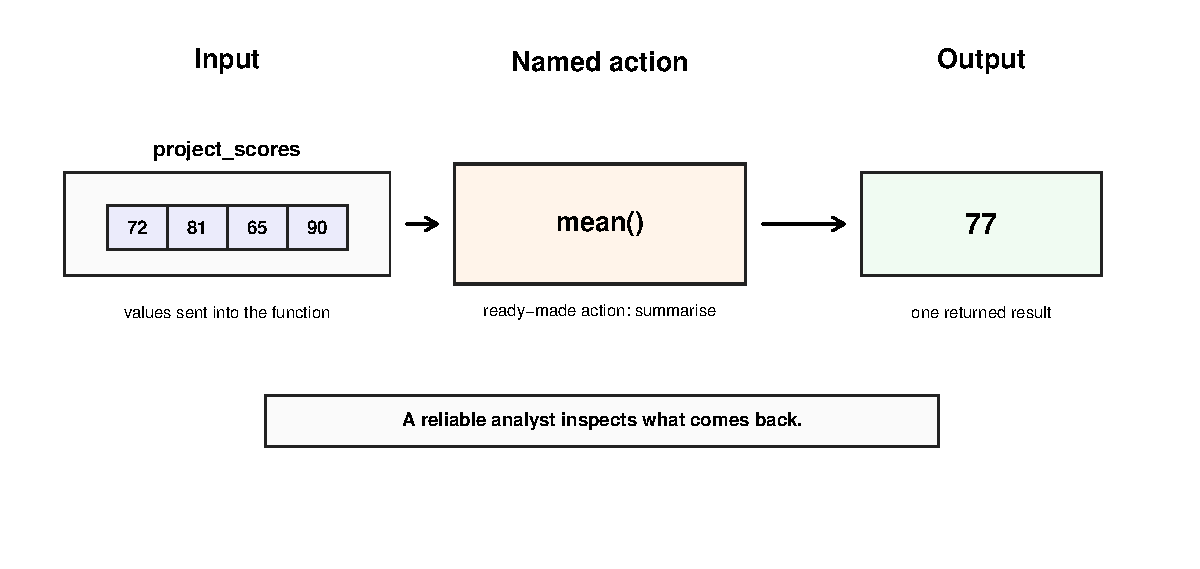
\includegraphics[width=0.9\linewidth,height=\textheight,keepaspectratio]{chapters/08-functions_files/figure-pdf/fig-function-input-action-output-1.pdf}

}

\caption{\label{fig-function-input-action-output}Input, Named Action,
and Output}

\end{figure}%

As shown in Figure~\ref{fig-function-input-action-output}, a function
call is not magic. \texttt{project\_scores} supplies the input.
\texttt{mean()} names the action. The output is the value returned by
that action.

This small model protects Leo from trying to memorise functions as
isolated commands. Each time he meets a new function, he can ask three
practical questions: What goes in? What action is being called? What
comes back?

\section{The Shape of a Function
Call}\label{the-shape-of-a-function-call}

A function call has a recognisable shape.

\begin{Shaded}
\begin{Highlighting}[]
\FunctionTok{round}\NormalTok{(}\FloatTok{82.567}\NormalTok{, }\AttributeTok{digits =} \DecValTok{2}\NormalTok{)}
\CommentTok{\#\textgreater{} [1] 82.57}
\end{Highlighting}
\end{Shaded}

In that line:

\begin{itemize}
\tightlist
\item
  \texttt{round} is the function name;
\item
  \texttt{82.567} is the main input;
\item
  \texttt{digits\ =\ 2} is an argument that shapes the action;
\item
  the parentheses contain the information the function needs;
\item
  the returned output is the rounded value.
\end{itemize}

The general form is:

\begin{Shaded}
\begin{Highlighting}[]
\NormalTok{function\_name(input, argument = value)}
\end{Highlighting}
\end{Shaded}

The name tells R which action to perform. The parentheses turn the name
into a call. The input and arguments tell R what to act on and how the
action should behave.

A missing parenthesis, wrong argument, wrong input type, or unexpected
missing value can change the result. Function literacy is not only
knowing names. It is reading the structure of the call.

\section{How R Thinks: Inputs, Action,
Output}\label{how-r-thinks-inputs-action-output}

When R meets a function call, it follows a practical sequence.

\begin{tcolorbox}[enhanced jigsaw, arc=.35mm, bottomrule=.15mm, breakable, colback=white, colframe=quarto-callout-tip-color-frame, left=2mm, leftrule=.75mm, opacityback=0, rightrule=.15mm, toprule=.15mm]
\begin{minipage}[t]{5.5mm}
\textcolor{quarto-callout-tip-color}{\faLightbulb}
\end{minipage}%
\begin{minipage}[t]{\textwidth - 5.5mm}

\vspace{-3mm}\textbf{How R Thinks}\vspace{3mm}

R looks for the function name, evaluates the inputs inside the
parentheses, sends those inputs to the function, and returns a result.
Leo's job is to inspect the result before he trusts it.

If the required inputs are missing or incompatible, the function may
return an error, warning, or unexpected result.

\end{minipage}%
\end{tcolorbox}

For example:

\begin{Shaded}
\begin{Highlighting}[]
\NormalTok{scores }\OtherTok{\textless{}{-}} \FunctionTok{c}\NormalTok{(}\DecValTok{72}\NormalTok{, }\DecValTok{81}\NormalTok{, }\DecValTok{65}\NormalTok{, }\DecValTok{90}\NormalTok{)}
\FunctionTok{mean}\NormalTok{(scores)}
\CommentTok{\#\textgreater{} [1] 77}
\end{Highlighting}
\end{Shaded}

R first finds \texttt{mean()}. It then evaluates \texttt{scores}, sends
the values into the function, and returns the average.

Calling the function is not the end of the work. A reliable analyst
checks what came back.

\section{Arguments: Instructions Inside the
Action}\label{arguments-instructions-inside-the-action}

Arguments tell a function how to behave.

Some functions need only one main input:

\begin{Shaded}
\begin{Highlighting}[]
\FunctionTok{length}\NormalTok{(scores)}
\CommentTok{\#\textgreater{} [1] 4}
\end{Highlighting}
\end{Shaded}

Some functions accept extra instructions:

\begin{Shaded}
\begin{Highlighting}[]
\FunctionTok{round}\NormalTok{(}\FloatTok{76.7525}\NormalTok{, }\AttributeTok{digits =} \DecValTok{2}\NormalTok{)}
\CommentTok{\#\textgreater{} [1] 76.75}
\end{Highlighting}
\end{Shaded}

The argument \texttt{digits\ =\ 2} tells \texttt{round()} how many
decimal places to keep.

Named arguments are often clearer for beginners because they make the
role of each value visible.

\begin{Shaded}
\begin{Highlighting}[]
\FunctionTok{round}\NormalTok{(}\AttributeTok{x =} \FloatTok{76.7525}\NormalTok{, }\AttributeTok{digits =} \DecValTok{2}\NormalTok{)}
\CommentTok{\#\textgreater{} [1] 76.75}
\end{Highlighting}
\end{Shaded}

A positional version can also work:

\begin{Shaded}
\begin{Highlighting}[]
\FunctionTok{round}\NormalTok{(}\FloatTok{76.7525}\NormalTok{, }\DecValTok{2}\NormalTok{)}
\CommentTok{\#\textgreater{} [1] 76.75}
\end{Highlighting}
\end{Shaded}

The second version is shorter, but the first version is easier to read.
In a serious workflow, clarity often matters more than saving a few
keystrokes.

When a function confuses Leo, one useful question is:

\begin{quote}
What is each argument doing?
\end{quote}

That question turns the call from a memorised spell into a readable
instruction.

\section{Predict Before You Run}\label{predict-before-you-run-3}

Prediction turns function use into reasoning.

Before running the next chunk, pause and answer two questions:

\begin{enumerate}
\def\labelenumi{\arabic{enumi}.}
\tightlist
\item
  Which function returns a summary value?
\item
  Which function counts how many values are present?
\end{enumerate}

\begin{Shaded}
\begin{Highlighting}[]
\NormalTok{project\_scores }\OtherTok{\textless{}{-}} \FunctionTok{c}\NormalTok{(}\DecValTok{72}\NormalTok{, }\DecValTok{81}\NormalTok{, }\DecValTok{65}\NormalTok{, }\DecValTok{90}\NormalTok{)}

\FunctionTok{mean}\NormalTok{(project\_scores)}
\CommentTok{\#\textgreater{} [1] 77}
\FunctionTok{length}\NormalTok{(project\_scores)}
\CommentTok{\#\textgreater{} [1] 4}
\end{Highlighting}
\end{Shaded}

\texttt{mean()} summarises the values into an average. \texttt{length()}
counts how many values are present. They both receive the same input,
but they perform different actions.

This is why function names matter. The input alone does not decide the
result. The action also matters.

\section{Inspect the Output Before You Trust
It}\label{inspect-the-output-before-you-trust-it}

Output inspection is part of reliable R work.

A function can return a number, text, a logical value, a vector, a
table-like object, a date, a plot, or something more complex. The
printed result may not tell the whole story.

Use inspection functions when the output matters:

\begin{Shaded}
\begin{Highlighting}[]
\NormalTok{average\_score }\OtherTok{\textless{}{-}} \FunctionTok{mean}\NormalTok{(project\_scores)}
\FunctionTok{class}\NormalTok{(average\_score)}
\CommentTok{\#\textgreater{} [1] "numeric"}
\FunctionTok{typeof}\NormalTok{(average\_score)}
\CommentTok{\#\textgreater{} [1] "double"}
\end{Highlighting}
\end{Shaded}

For larger objects, Leo may use functions such as:

\begin{Shaded}
\begin{Highlighting}[]
\FunctionTok{str}\NormalTok{(project\_scores)}
\CommentTok{\#\textgreater{}  num [1:4] 72 81 65 90}
\FunctionTok{summary}\NormalTok{(project\_scores)}
\CommentTok{\#\textgreater{}    Min. 1st Qu.  Median    Mean 3rd Qu.    Max. }
\CommentTok{\#\textgreater{}   65.00   70.25   76.50   77.00   83.25   90.00}
\FunctionTok{length}\NormalTok{(project\_scores)}
\CommentTok{\#\textgreater{} [1] 4}
\FunctionTok{is.na}\NormalTok{(project\_scores)}
\CommentTok{\#\textgreater{} [1] FALSE FALSE FALSE FALSE}
\end{Highlighting}
\end{Shaded}

summary() adapts its output to the kind of object it receives.

These functions are small, but they create a serious habit: inspect
before trust.

\begin{tcolorbox}[enhanced jigsaw, arc=.35mm, bottomrule=.15mm, breakable, colback=white, colframe=quarto-callout-important-color-frame, left=2mm, leftrule=.75mm, opacityback=0, rightrule=.15mm, toprule=.15mm]
\begin{minipage}[t]{5.5mm}
\textcolor{quarto-callout-important-color}{\faExclamation}
\end{minipage}%
\begin{minipage}[t]{\textwidth - 5.5mm}

\vspace{-3mm}\textbf{Reliable Analysis Rule}\vspace{3mm}

Calling a function is not the end of the work. A reliable analyst checks
what came back.

\end{minipage}%
\end{tcolorbox}

\section{A Beginner Core of Built-in
Functions}\label{a-beginner-core-of-built-in-functions}

R contains many functions. Chapter 8 does not need to become a
dictionary.

For now, Leo needs a beginner core: functions that help him combine,
inspect, check, convert, summarise, handle missing values, work with
text, and work with dates. These are the functions that appear again and
again in practical data work.

The advanced families still matter, but they do not all belong in Leo's
everyday toolkit yet. They will make more sense when a real need
appears.

The next sections focus on this beginner core.

\section{Combining and Measuring
Values}\label{combining-and-measuring-values}

The function \texttt{c()} combines values.

\begin{Shaded}
\begin{Highlighting}[]
\NormalTok{study\_hours }\OtherTok{\textless{}{-}} \FunctionTok{c}\NormalTok{(}\DecValTok{5}\NormalTok{, }\DecValTok{7}\NormalTok{, }\DecValTok{4}\NormalTok{, }\DecValTok{8}\NormalTok{)}
\NormalTok{study\_hours}
\CommentTok{\#\textgreater{} [1] 5 7 4 8}
\end{Highlighting}
\end{Shaded}

The function \texttt{length()} measures how many values are present.

\begin{Shaded}
\begin{Highlighting}[]
\FunctionTok{length}\NormalTok{(study\_hours)}
\CommentTok{\#\textgreater{} [1] 4}
\end{Highlighting}
\end{Shaded}

The function \texttt{seq()} creates a sequence.

\begin{Shaded}
\begin{Highlighting}[]
\FunctionTok{seq}\NormalTok{(}\AttributeTok{from =} \DecValTok{1}\NormalTok{, }\AttributeTok{to =} \DecValTok{5}\NormalTok{)}
\CommentTok{\#\textgreater{} [1] 1 2 3 4 5}
\end{Highlighting}
\end{Shaded}

The function \texttt{rep()} repeats values.

\begin{Shaded}
\begin{Highlighting}[]
\FunctionTok{rep}\NormalTok{(}\StringTok{"practice"}\NormalTok{, }\AttributeTok{times =} \DecValTok{3}\NormalTok{)}
\CommentTok{\#\textgreater{} [1] "practice" "practice" "practice"}
\end{Highlighting}
\end{Shaded}

These functions are not dramatic, but they are foundational. They help
Leo create and check small objects before working with larger data.

\section{Summarising Values}\label{summarising-values}

Summary functions reduce many values into a smaller result.

\begin{Shaded}
\begin{Highlighting}[]
\NormalTok{project\_scores }\OtherTok{\textless{}{-}} \FunctionTok{c}\NormalTok{(}\DecValTok{72}\NormalTok{, }\DecValTok{81}\NormalTok{, }\DecValTok{65}\NormalTok{, }\DecValTok{90}\NormalTok{)}

\FunctionTok{sum}\NormalTok{(project\_scores)}
\CommentTok{\#\textgreater{} [1] 308}
\FunctionTok{min}\NormalTok{(project\_scores)}
\CommentTok{\#\textgreater{} [1] 65}
\FunctionTok{max}\NormalTok{(project\_scores)}
\CommentTok{\#\textgreater{} [1] 90}
\FunctionTok{range}\NormalTok{(project\_scores)}
\CommentTok{\#\textgreater{} [1] 65 90}
\FunctionTok{mean}\NormalTok{(project\_scores)}
\CommentTok{\#\textgreater{} [1] 77}
\FunctionTok{median}\NormalTok{(project\_scores)}
\CommentTok{\#\textgreater{} [1] 76.5}
\end{Highlighting}
\end{Shaded}

Each function answers a different question.

\texttt{sum()} asks for the total. \texttt{max()} asks for the highest
value. \texttt{range()} asks for the lowest and highest values. It
returns both values together as a vector. \texttt{mean()} asks for the
average. \texttt{median()} asks for the middle value.

Logical summaries connect directly to Chapter 7.

\begin{Shaded}
\begin{Highlighting}[]
\NormalTok{passed }\OtherTok{\textless{}{-}}\NormalTok{ project\_scores }\SpecialCharTok{\textgreater{}=} \DecValTok{70}
\FunctionTok{any}\NormalTok{(passed)}
\CommentTok{\#\textgreater{} [1] TRUE}
\FunctionTok{all}\NormalTok{(passed)}
\CommentTok{\#\textgreater{} [1] FALSE}
\end{Highlighting}
\end{Shaded}

\texttt{any()} asks whether at least one value is \texttt{TRUE}.
\texttt{all()} asks whether every value is \texttt{TRUE}.

This is a useful bridge. Chapter 7 taught Leo how R makes judgments.
Chapter 8 shows how functions can summarise those judgments.

\section{Working with Missing Values}\label{working-with-missing-values}

Real data often contains \texttt{NA}.

\begin{Shaded}
\begin{Highlighting}[]
\NormalTok{scores\_with\_na }\OtherTok{\textless{}{-}} \FunctionTok{c}\NormalTok{(}\DecValTok{72}\NormalTok{, }\DecValTok{81}\NormalTok{, }\ConstantTok{NA}\NormalTok{, }\DecValTok{90}\NormalTok{)}
\FunctionTok{mean}\NormalTok{(scores\_with\_na)}
\CommentTok{\#\textgreater{} [1] NA}
\end{Highlighting}
\end{Shaded}

R returns \texttt{NA} because one value is missing. The function is not
broken. It is being cautious because the average cannot be known
completely from the available values unless Leo decides how to handle
the missing value.

One common argument is \texttt{na.rm\ =\ TRUE}.

\begin{Shaded}
\begin{Highlighting}[]
\FunctionTok{mean}\NormalTok{(scores\_with\_na, }\AttributeTok{na.rm =} \ConstantTok{TRUE}\NormalTok{)}
\CommentTok{\#\textgreater{} [1] 81}
\end{Highlighting}
\end{Shaded}

The argument means: remove missing values before calculating.

The same pattern appears in several summary functions:

\begin{Shaded}
\begin{Highlighting}[]
\FunctionTok{sum}\NormalTok{(scores\_with\_na, }\AttributeTok{na.rm =} \ConstantTok{TRUE}\NormalTok{)}
\CommentTok{\#\textgreater{} [1] 243}
\FunctionTok{min}\NormalTok{(scores\_with\_na, }\AttributeTok{na.rm =} \ConstantTok{TRUE}\NormalTok{)}
\CommentTok{\#\textgreater{} [1] 72}
\FunctionTok{max}\NormalTok{(scores\_with\_na, }\AttributeTok{na.rm =} \ConstantTok{TRUE}\NormalTok{)}
\CommentTok{\#\textgreater{} [1] 90}
\end{Highlighting}
\end{Shaded}

But \texttt{na.rm\ =\ TRUE} is not an automatic repair. It is an
analytical decision.

\begin{tcolorbox}[enhanced jigsaw, arc=.35mm, bottomrule=.15mm, breakable, colback=white, colframe=quarto-callout-warning-color-frame, left=2mm, leftrule=.75mm, opacityback=0, rightrule=.15mm, toprule=.15mm]
\begin{minipage}[t]{5.5mm}
\textcolor{quarto-callout-warning-color}{\faExclamationTriangle}
\end{minipage}%
\begin{minipage}[t]{\textwidth - 5.5mm}

\vspace{-3mm}\textbf{Common Beginner Trap}\vspace{3mm}

Do not treat \texttt{na.rm\ =\ TRUE} as a magic fix. It removes missing
values from that calculation. It does not explain why the values are
missing or whether excluding them is appropriate.

\end{minipage}%
\end{tcolorbox}

Special values require special care. The function can help, but the
analyst still owns the decision.

\section{Checking and Converting
Values}\label{checking-and-converting-values}

Checking functions ask what an object is.

\begin{Shaded}
\begin{Highlighting}[]
\FunctionTok{is.numeric}\NormalTok{(}\DecValTok{25}\NormalTok{)}
\CommentTok{\#\textgreater{} [1] TRUE}
\FunctionTok{is.character}\NormalTok{(}\StringTok{"Nigeria"}\NormalTok{)}
\CommentTok{\#\textgreater{} [1] TRUE}
\FunctionTok{is.logical}\NormalTok{(}\ConstantTok{TRUE}\NormalTok{)}
\CommentTok{\#\textgreater{} [1] TRUE}
\FunctionTok{is.na}\NormalTok{(}\ConstantTok{NA}\NormalTok{)}
\CommentTok{\#\textgreater{} [1] TRUE}
\end{Highlighting}
\end{Shaded}

Conversion functions attempt to change values.

\begin{Shaded}
\begin{Highlighting}[]
\FunctionTok{as.numeric}\NormalTok{(}\StringTok{"25"}\NormalTok{)}
\CommentTok{\#\textgreater{} [1] 25}
\FunctionTok{as.character}\NormalTok{(}\DecValTok{25}\NormalTok{)}
\CommentTok{\#\textgreater{} [1] "25"}
\FunctionTok{as.logical}\NormalTok{(}\DecValTok{1}\NormalTok{)}
\CommentTok{\#\textgreater{} [1] TRUE}
\end{Highlighting}
\end{Shaded}

Numeric conversion to logical follows R's coercion rules: 0 becomes
FALSE, and non-zero values become TRUE.

Conversion can also fail.

Before running the next chunk, predict what will happen. Which
conversion succeeds? Which one produces a warning?

\begin{Shaded}
\begin{Highlighting}[]
\FunctionTok{as.numeric}\NormalTok{(}\StringTok{"Leo"}\NormalTok{)}
\CommentTok{\#\textgreater{} Warning: NAs introduced by coercion}
\CommentTok{\#\textgreater{} [1] NA}
\end{Highlighting}
\end{Shaded}

R cannot turn the word \texttt{"Leo"} into a meaningful number, so it
returns \texttt{NA} and warns the user. That warning is useful
information. A failed conversion can introduce missing values into an
analysis.

A safer habit is:

\begin{Shaded}
\begin{Highlighting}[]
\NormalTok{inspect → convert → inspect again}
\end{Highlighting}
\end{Shaded}

The habit is small. The protection is large.

\section{Working with Text}\label{working-with-text}

Text data appears constantly in real datasets: names, countries,
categories, labels, comments, and identifiers.

Create a small text value:

\begin{Shaded}
\begin{Highlighting}[]
\NormalTok{country }\OtherTok{\textless{}{-}} \StringTok{" Nigeria "}
\end{Highlighting}
\end{Shaded}

Remove leading and trailing spaces:

\begin{Shaded}
\begin{Highlighting}[]
\FunctionTok{trimws}\NormalTok{(country)}
\CommentTok{\#\textgreater{} [1] "Nigeria"}
\end{Highlighting}
\end{Shaded}

Standardise case:

\begin{Shaded}
\begin{Highlighting}[]
\FunctionTok{tolower}\NormalTok{(country)}
\CommentTok{\#\textgreater{} [1] " nigeria "}
\FunctionTok{toupper}\NormalTok{(country)}
\CommentTok{\#\textgreater{} [1] " NIGERIA "}
\end{Highlighting}
\end{Shaded}

Count characters:

\begin{Shaded}
\begin{Highlighting}[]
\FunctionTok{nchar}\NormalTok{(country)}
\CommentTok{\#\textgreater{} [1] 9}
\end{Highlighting}
\end{Shaded}

Join text:

\begin{Shaded}
\begin{Highlighting}[]
\FunctionTok{paste}\NormalTok{(}\StringTok{"Hello"}\NormalTok{, }\StringTok{"Leo"}\NormalTok{)}
\CommentTok{\#\textgreater{} [1] "Hello Leo"}
\FunctionTok{paste0}\NormalTok{(}\StringTok{"ID\_"}\NormalTok{, }\DecValTok{1001}\NormalTok{)}
\CommentTok{\#\textgreater{} [1] "ID\_1001"}
\end{Highlighting}
\end{Shaded}

Find a pattern:

\begin{Shaded}
\begin{Highlighting}[]
\FunctionTok{grepl}\NormalTok{(}\StringTok{"Nig"}\NormalTok{, country)}
\CommentTok{\#\textgreater{} [1] TRUE}
\end{Highlighting}
\end{Shaded}

Replace text:

\begin{Shaded}
\begin{Highlighting}[]
\FunctionTok{gsub}\NormalTok{(}\StringTok{"Nigeria"}\NormalTok{, }\StringTok{"NG"}\NormalTok{, }\FunctionTok{trimws}\NormalTok{(country))}
\CommentTok{\#\textgreater{} [1] "NG"}
\end{Highlighting}
\end{Shaded}

Text functions quickly become practical. \texttt{"Nigeria"},
\texttt{"\ Nigeria"}, \texttt{"nigeria"}, and \texttt{"NIGERIA"} may
look like the same country to a human reader, but R does not
automatically treat them as identical.

For now, the action map is simple: trim, change case, count, join, find,
and replace.

\section{Working with Dates}\label{working-with-dates}

Dates may look like text, but R needs date objects to calculate time
correctly.

\begin{Shaded}
\begin{Highlighting}[]
\NormalTok{enrolment\_date }\OtherTok{\textless{}{-}} \FunctionTok{as.Date}\NormalTok{(}\StringTok{"2026{-}04{-}28"}\NormalTok{)}
\NormalTok{enrolment\_date}
\CommentTok{\#\textgreater{} [1] "2026{-}04{-}28"}
\FunctionTok{class}\NormalTok{(enrolment\_date)}
\CommentTok{\#\textgreater{} [1] "Date"}
\end{Highlighting}
\end{Shaded}

A date stored as text may print neatly, but it will not behave like a
real date in ordering, comparison, filtering, or time differences.

Calculate a time difference:

\begin{Shaded}
\begin{Highlighting}[]
\NormalTok{start\_date }\OtherTok{\textless{}{-}} \FunctionTok{as.Date}\NormalTok{(}\StringTok{"2026{-}04{-}01"}\NormalTok{)}
\NormalTok{end\_date }\OtherTok{\textless{}{-}} \FunctionTok{as.Date}\NormalTok{(}\StringTok{"2026{-}04{-}28"}\NormalTok{)}

\NormalTok{end\_date }\SpecialCharTok{{-}}\NormalTok{ start\_date}
\CommentTok{\#\textgreater{} Time difference of 27 days}
\end{Highlighting}
\end{Shaded}

Format a date for display:

\begin{Shaded}
\begin{Highlighting}[]
\FunctionTok{format}\NormalTok{(enrolment\_date, }\StringTok{"\%B \%d, \%Y"}\NormalTok{)}
\CommentTok{\#\textgreater{} [1] "April 28, 2026"}
\end{Highlighting}
\end{Shaded}

Create a short date sequence:

\begin{Shaded}
\begin{Highlighting}[]
\FunctionTok{seq.Date}\NormalTok{(}
  \AttributeTok{from =} \FunctionTok{as.Date}\NormalTok{(}\StringTok{"2026{-}04{-}01"}\NormalTok{),}
  \AttributeTok{to =} \FunctionTok{as.Date}\NormalTok{(}\StringTok{"2026{-}04{-}05"}\NormalTok{),}
  \AttributeTok{by =} \StringTok{"day"}
\NormalTok{)}
\CommentTok{\#\textgreater{} [1] "2026{-}04{-}01" "2026{-}04{-}02" "2026{-}04{-}03" "2026{-}04{-}04" "2026{-}04{-}05"}
\end{Highlighting}
\end{Shaded}

The key lesson is not advanced date handling. The lesson is that
functions can turn date-like text into date-aware values and then
perform time-aware actions.

\section{Simple Formatting and
Sampling}\label{simple-formatting-and-sampling}

Formatting controls display.

\begin{Shaded}
\begin{Highlighting}[]
\NormalTok{score\_value }\OtherTok{\textless{}{-}} \FloatTok{82.567}
\FunctionTok{round}\NormalTok{(score\_value, }\AttributeTok{digits =} \DecValTok{2}\NormalTok{)}
\CommentTok{\#\textgreater{} [1] 82.57}
\end{Highlighting}
\end{Shaded}

Some formatting functions return text.

\begin{Shaded}
\begin{Highlighting}[]
\NormalTok{formatted\_score }\OtherTok{\textless{}{-}} \FunctionTok{sprintf}\NormalTok{(}\StringTok{"\%.2f"}\NormalTok{, score\_value)}
\NormalTok{formatted\_score}
\CommentTok{\#\textgreater{} [1] "82.57"}
\FunctionTok{class}\NormalTok{(formatted\_score)}
\CommentTok{\#\textgreater{} [1] "character"}
\end{Highlighting}
\end{Shaded}

This is useful for labels and reports, but it matters if Leo wants to
calculate later. A value that looks numeric after formatting may be
character text.

Sampling creates selected values.

Random sampling normally changes each time the code runs.

\begin{Shaded}
\begin{Highlighting}[]
\NormalTok{learner\_ids }\OtherTok{\textless{}{-}} \FunctionTok{paste0}\NormalTok{(}\StringTok{"L"}\NormalTok{, }\DecValTok{1001}\SpecialCharTok{:}\DecValTok{1005}\NormalTok{)}
\FunctionTok{set.seed}\NormalTok{(}\DecValTok{123}\NormalTok{)}
\FunctionTok{sample}\NormalTok{(learner\_ids, }\AttributeTok{size =} \DecValTok{2}\NormalTok{)}
\CommentTok{\#\textgreater{} [1] "L1003" "L1002"}
\end{Highlighting}
\end{Shaded}

set.seed() fixes the random starting point so the same sample can be
reproduced.

\texttt{set.seed()} makes this random-looking result reproducible. When
randomness enters a workflow, reproducibility needs attention.

\section{A Small Momentum Win}\label{a-small-momentum-win}

Now Leo can use several built-in functions together without doing full
data analysis.

\begin{Shaded}
\begin{Highlighting}[]
\NormalTok{project\_scores }\OtherTok{\textless{}{-}} \FunctionTok{c}\NormalTok{(}\DecValTok{72}\NormalTok{, }\DecValTok{81}\NormalTok{, }\DecValTok{65}\NormalTok{, }\DecValTok{90}\NormalTok{)}
\NormalTok{study\_hours }\OtherTok{\textless{}{-}} \FunctionTok{c}\NormalTok{(}\DecValTok{5}\NormalTok{, }\DecValTok{7}\NormalTok{, }\DecValTok{4}\NormalTok{, }\DecValTok{8}\NormalTok{)}

\FunctionTok{mean}\NormalTok{(project\_scores)}
\CommentTok{\#\textgreater{} [1] 77}
\FunctionTok{max}\NormalTok{(project\_scores)}
\CommentTok{\#\textgreater{} [1] 90}
\FunctionTok{length}\NormalTok{(project\_scores)}
\CommentTok{\#\textgreater{} [1] 4}
\end{Highlighting}
\end{Shaded}

He can round a summary:

\begin{Shaded}
\begin{Highlighting}[]
\FunctionTok{round}\NormalTok{(}\FunctionTok{mean}\NormalTok{(project\_scores), }\AttributeTok{digits =} \DecValTok{1}\NormalTok{)}
\CommentTok{\#\textgreater{} [1] 77}
\end{Highlighting}
\end{Shaded}

He can use Chapter 7 logic and then summarise the judgments:

\begin{Shaded}
\begin{Highlighting}[]
\NormalTok{high\_scores }\OtherTok{\textless{}{-}}\NormalTok{ project\_scores }\SpecialCharTok{\textgreater{}=} \DecValTok{80}
\NormalTok{high\_scores}
\CommentTok{\#\textgreater{} [1] FALSE  TRUE FALSE  TRUE}
\FunctionTok{sum}\NormalTok{(high\_scores)}
\CommentTok{\#\textgreater{} [1] 2}
\end{Highlighting}
\end{Shaded}

He can calculate a simple ratio and make it readable:

\begin{Shaded}
\begin{Highlighting}[]
\NormalTok{score\_per\_hour }\OtherTok{\textless{}{-}}\NormalTok{ project\_scores }\SpecialCharTok{/}\NormalTok{ study\_hours}
\FunctionTok{round}\NormalTok{(score\_per\_hour, }\AttributeTok{digits =} \DecValTok{2}\NormalTok{)}
\CommentTok{\#\textgreater{} [1] 14.40 11.57 16.25 11.25}
\end{Highlighting}
\end{Shaded}

This is still a small example. But it is no longer only syntax practice.
Leo has used ready-made actions to inspect, summarise, compare, and
report a small set of learner values.

That is a momentum win.

\section{A Practical Map of Built-in Function
Families}\label{a-practical-map-of-built-in-function-families}

This map is not a memorisation list.

Leo does not need to master every function family in one sitting. The
purpose of the map is to help him recognise that functions have jobs.
Some inspect objects. Some summarise values. Some transform text. Some
work with dates. Some help with randomness, formatting, matrices,
graphics, files, or the R session itself.

For now, Leo should focus on the beginner core: combining, inspecting,
checking, converting, summarising, handling missing values, working with
text, and working with dates. The remaining families are previews. They
are included so that later chapters feel connected, not so that Leo has
to memorise them immediately.

\begin{longtable}[]{@{}
  >{\raggedright\arraybackslash}p{(\linewidth - 6\tabcolsep) * \real{0.2500}}
  >{\raggedright\arraybackslash}p{(\linewidth - 6\tabcolsep) * \real{0.2500}}
  >{\raggedright\arraybackslash}p{(\linewidth - 6\tabcolsep) * \real{0.2500}}
  >{\raggedright\arraybackslash}p{(\linewidth - 6\tabcolsep) * \real{0.2500}}@{}}
\caption{A beginner map of useful built-in function
families}\label{tbl-function-families}\tabularnewline
\toprule\noalign{}
\begin{minipage}[b]{\linewidth}\raggedright
Tier
\end{minipage} & \begin{minipage}[b]{\linewidth}\raggedright
Function family
\end{minipage} & \begin{minipage}[b]{\linewidth}\raggedright
Examples
\end{minipage} & \begin{minipage}[b]{\linewidth}\raggedright
Beginner purpose
\end{minipage} \\
\midrule\noalign{}
\endfirsthead
\toprule\noalign{}
\begin{minipage}[b]{\linewidth}\raggedright
Tier
\end{minipage} & \begin{minipage}[b]{\linewidth}\raggedright
Function family
\end{minipage} & \begin{minipage}[b]{\linewidth}\raggedright
Examples
\end{minipage} & \begin{minipage}[b]{\linewidth}\raggedright
Beginner purpose
\end{minipage} \\
\midrule\noalign{}
\endhead
\bottomrule\noalign{}
\endlastfoot
Beginner core & Combine and measure & \texttt{c()}, \texttt{length()},
\texttt{seq()}, \texttt{rep()} & Create and check small objects \\
Beginner core & Inspect objects & \texttt{str()}, \texttt{class()},
\texttt{typeof()}, \texttt{summary()} & See what R sees \\
Beginner core & Summarise values & \texttt{sum()}, \texttt{mean()},
\texttt{median()}, \texttt{min()}, \texttt{max()} & Reduce values into
useful summaries \\
Beginner core & Handle missing values & \texttt{is.na()},
\texttt{complete.cases()}, \texttt{na.rm\ =\ TRUE} & Find or manage
missingness carefully \\
Beginner core & Check and convert & \texttt{is.numeric()},
\texttt{as.numeric()}, \texttt{as.character()} & Confirm or change what
R is working with \\
Beginner core & Work with text & \texttt{trimws()}, \texttt{tolower()},
\texttt{paste()}, \texttt{grepl()}, \texttt{gsub()} & Clean and prepare
simple text values \\
Beginner core & Work with dates & \texttt{as.Date()}, \texttt{format()},
\texttt{seq.Date()} & Turn date-like values into date-aware values \\
Useful soon & Format and sample & \texttt{round()}, \texttt{sprintf()},
\texttt{sample()}, \texttt{set.seed()} & Prepare output and make
examples reproducible \\
Preview only & Repeat actions & \texttt{lapply()}, \texttt{sapply()},
\texttt{apply()} & Repeat a function across objects or structures \\
Preview only & Diagnose and protect workflows & \texttt{traceback()},
\texttt{debug()}, \texttt{tryCatch()}, \texttt{stop()},
\texttt{warning()} & Investigate or respond to problems later \\
Preview only & Work with files, sessions, packages, and systems &
\texttt{getwd()}, \texttt{list.files()}, \texttt{sessionInfo()},
\texttt{library()} & Manage larger workflows later \\
\end{longtable}

The table gives orientation. It is not a test.

A learner who memorises names becomes anxious when a new function
appears. A learner with a map asks a better question:

\begin{quote}
What job is this function trying to do?
\end{quote}

\section{Reference Preview: Functions for
Later}\label{reference-preview-functions-for-later}

Some functions matter later but do not belong in Leo's everyday beginner
toolkit yet.

These include tools for:

\begin{itemize}
\tightlist
\item
  repeating actions across structures;
\item
  debugging workflows;
\item
  handling warnings and errors;
\item
  working with files and sessions;
\item
  producing graphics.
\end{itemize}

Leo will learn these when the workflow creates a real need for them.

\section{Functions, Operators, and Language Constructs Are Not the
Same}\label{functions-operators-and-language-constructs-are-not-the-same}

Before leaving Chapter 8, Leo needs one more boundary.

Not every ready-made R tool is a function.

Operators shape expressions:

\begin{Shaded}
\begin{Highlighting}[]
\DecValTok{10} \SpecialCharTok{+} \DecValTok{5}
\NormalTok{score }\SpecialCharTok{\textgreater{}=} \DecValTok{50}
\NormalTok{x }\OtherTok{\textless{}{-}} \DecValTok{10}
\end{Highlighting}
\end{Shaded}

Language constructs control execution:

\begin{Shaded}
\begin{Highlighting}[]
\ControlFlowTok{if}
\ControlFlowTok{else}
\ControlFlowTok{for}
\ControlFlowTok{while}
\ControlFlowTok{next}
\ControlFlowTok{break}
\end{Highlighting}
\end{Shaded}

Functions perform named reusable actions:

\begin{Shaded}
\begin{Highlighting}[]
\FunctionTok{mean}\NormalTok{(project\_scores)}
\FunctionTok{round}\NormalTok{(}\FloatTok{82.567}\NormalTok{, }\AttributeTok{digits =} \DecValTok{2}\NormalTok{)}
\FunctionTok{tolower}\NormalTok{(}\StringTok{"Nigeria"}\NormalTok{)}
\end{Highlighting}
\end{Shaded}

These categories often work together. A function can receive a logical
expression as an argument. An operator can appear inside a function
call. A language construct can decide whether a function runs. But their
roles are not identical.

Chapter 7 taught operators and logic. Chapter 8 teaches functions.
Chapter 9 will show how Leo can create small named actions of his own.

\section{Built-in Functions Are Not the Whole R
Ecosystem}\label{built-in-functions-are-not-the-whole-r-ecosystem}

R also has package-based functions.

Later, Leo will meet functions such as:

\begin{Shaded}
\begin{Highlighting}[]
\FunctionTok{filter}\NormalTok{()}
\FunctionTok{select}\NormalTok{()}
\FunctionTok{mutate}\NormalTok{()}
\FunctionTok{summarise}\NormalTok{()}
\FunctionTok{ggplot}\NormalTok{()}
\end{Highlighting}
\end{Shaded}

Those functions usually come from packages such as \texttt{dplyr} and
\texttt{ggplot2}.

This does not mean package functions rescue Leo from Base R. A better
frame is:

\begin{quote}
Base R teaches the structure of the language. Tidyverse later provides a
different grammar for expressing common data workflows. Many R users
benefit from understanding both approaches.
\end{quote}

The package may change, but the basic function questions remain the
same:

\begin{itemize}
\tightlist
\item
  What is the function name?
\item
  What input goes in?
\item
  What arguments shape the action?
\item
  What output comes back?
\item
  Does the result make sense?
\end{itemize}

Once that model is secure, package functions become less intimidating.

\section{How to Ask for Help}\label{how-to-ask-for-help}

R has built-in help.

\begin{Shaded}
\begin{Highlighting}[]
\NormalTok{?mean}
\FunctionTok{help}\NormalTok{(mean)}
\NormalTok{??correlation}
\end{Highlighting}
\end{Shaded}

Documentation can look dense at first. Leo does not need to understand
every line immediately. He can begin with practical questions:

\begin{itemize}
\tightlist
\item
  What does the function do?
\item
  What arguments does it accept?
\item
  Which arguments have default values?
\item
  What kind of output does it return?
\item
  What examples appear near the bottom?
\end{itemize}

\begin{tcolorbox}[enhanced jigsaw, arc=.35mm, bottomrule=.15mm, breakable, colback=white, colframe=quarto-callout-tip-color-frame, left=2mm, leftrule=.75mm, opacityback=0, rightrule=.15mm, toprule=.15mm]
\begin{minipage}[t]{5.5mm}
\textcolor{quarto-callout-tip-color}{\faLightbulb}
\end{minipage}%
\begin{minipage}[t]{\textwidth - 5.5mm}

\vspace{-3mm}\textbf{Professional Function Literacy}\vspace{3mm}

A professional R user does not remember everything. A professional R
user knows how to investigate.

\end{minipage}%
\end{tcolorbox}

That is how Leo becomes less dependent on copied code: inspect the help
page, test a small example, and check the output.

\section{Common Beginner Mistakes}\label{common-beginner-mistakes-1}

Mistakes with functions are normal. The goal is to recognise the pattern
and repair it before it spreads.

\begin{longtable}[]{@{}
  >{\raggedright\arraybackslash}p{(\linewidth - 4\tabcolsep) * \real{0.3333}}
  >{\raggedright\arraybackslash}p{(\linewidth - 4\tabcolsep) * \real{0.3333}}
  >{\raggedright\arraybackslash}p{(\linewidth - 4\tabcolsep) * \real{0.3333}}@{}}
\caption{Common beginner mistakes when using
functions}\label{tbl-function-mistakes}\tabularnewline
\toprule\noalign{}
\begin{minipage}[b]{\linewidth}\raggedright
Mistake
\end{minipage} & \begin{minipage}[b]{\linewidth}\raggedright
What goes wrong
\end{minipage} & \begin{minipage}[b]{\linewidth}\raggedright
Safer habit
\end{minipage} \\
\midrule\noalign{}
\endfirsthead
\toprule\noalign{}
\begin{minipage}[b]{\linewidth}\raggedright
Mistake
\end{minipage} & \begin{minipage}[b]{\linewidth}\raggedright
What goes wrong
\end{minipage} & \begin{minipage}[b]{\linewidth}\raggedright
Safer habit
\end{minipage} \\
\midrule\noalign{}
\endhead
\bottomrule\noalign{}
\endlastfoot
Forgetting parentheses & R sees a name, not a function call & Use
\texttt{mean(scores)}, not \texttt{mean\ scores} \\
Supplying the wrong type & The function receives values it cannot use
properly & Check with \texttt{class()} or \texttt{str()} \\
Ignoring missing values & Summary functions may return \texttt{NA} &
Inspect missingness before using \texttt{na.rm\ =\ TRUE} \\
Confusing display with type & A formatted result may be character text &
Check the class after formatting \\
Treating every tool as a function & Operators and language constructs
follow different rules & Ask what role the tool is playing \\
Hiding errors too early & Error handling can conceal a problem &
Understand the error before protecting against it \\
\end{longtable}

One example is worth seeing again. This looks tidy:

\begin{Shaded}
\begin{Highlighting}[]
\FunctionTok{sprintf}\NormalTok{(}\StringTok{"\%.2f"}\NormalTok{, }\FloatTok{82.567}\NormalTok{)}
\CommentTok{\#\textgreater{} [1] "82.57"}
\end{Highlighting}
\end{Shaded}

But the result is text.

\begin{Shaded}
\begin{Highlighting}[]
\FunctionTok{class}\NormalTok{(}\FunctionTok{sprintf}\NormalTok{(}\StringTok{"\%.2f"}\NormalTok{, }\FloatTok{82.567}\NormalTok{))}
\CommentTok{\#\textgreater{} [1] "character"}
\end{Highlighting}
\end{Shaded}

The screen shows appearance. Inspection reveals behaviour.

\section{What Leo Is Expected to Know at This
Point}\label{what-leo-is-expected-to-know-at-this-point-3}

\begin{tcolorbox}[enhanced jigsaw, arc=.35mm, bottomrule=.15mm, breakable, colback=white, colframe=quarto-callout-note-color-frame, left=2mm, leftrule=.75mm, opacityback=0, rightrule=.15mm, toprule=.15mm]
\begin{minipage}[t]{5.5mm}
\textcolor{quarto-callout-note-color}{\faInfo}
\end{minipage}%
\begin{minipage}[t]{\textwidth - 5.5mm}

\vspace{-3mm}\textbf{Not Yet}\vspace{3mm}

Leo is not expected to memorise the function catalogue, understand
advanced evaluation, use \texttt{tryCatch()}, master the apply family,
build package workflows, or write his own functions yet.

He is expected to understand the function model: name, input, arguments,
action, output, and inspection.

\end{minipage}%
\end{tcolorbox}

That is enough for this chapter.

\section{A Small Practice Lab}\label{a-small-practice-lab}

Create these objects:

\begin{Shaded}
\begin{Highlighting}[]
\NormalTok{scores }\OtherTok{\textless{}{-}} \FunctionTok{c}\NormalTok{(}\DecValTok{70}\NormalTok{, }\DecValTok{82}\NormalTok{, }\DecValTok{91}\NormalTok{, }\DecValTok{64}\NormalTok{, }\ConstantTok{NA}\NormalTok{)}
\NormalTok{country }\OtherTok{\textless{}{-}} \StringTok{" Nigeria "}
\end{Highlighting}
\end{Shaded}

Before running each function, predict what kind of output it will
return.

\begin{Shaded}
\begin{Highlighting}[]
\FunctionTok{length}\NormalTok{(scores)}
\CommentTok{\#\textgreater{} [1] 5}
\FunctionTok{summary}\NormalTok{(scores)}
\CommentTok{\#\textgreater{}    Min. 1st Qu.  Median    Mean 3rd Qu.    Max.    NA\textquotesingle{}s }
\CommentTok{\#\textgreater{}   64.00   68.50   76.00   76.75   84.25   91.00       1}
\FunctionTok{mean}\NormalTok{(scores, }\AttributeTok{na.rm =} \ConstantTok{TRUE}\NormalTok{)}
\CommentTok{\#\textgreater{} [1] 76.75}
\FunctionTok{round}\NormalTok{(}\FunctionTok{mean}\NormalTok{(scores, }\AttributeTok{na.rm =} \ConstantTok{TRUE}\NormalTok{), }\AttributeTok{digits =} \DecValTok{1}\NormalTok{)}
\CommentTok{\#\textgreater{} [1] 76.8}
\FunctionTok{trimws}\NormalTok{(country)}
\CommentTok{\#\textgreater{} [1] "Nigeria"}
\FunctionTok{tolower}\NormalTok{(country)}
\CommentTok{\#\textgreater{} [1] " nigeria "}
\end{Highlighting}
\end{Shaded}

Now reflect:

\begin{itemize}
\tightlist
\item
  Which functions inspected?
\item
  Which functions summarised?
\item
  Which functions transformed display or text?
\item
  Which function needed a missing-value decision?
\item
  Which outputs would you inspect before using them in a report?
\end{itemize}

The point is not speed. The point is recognition.

\section{Chapter Outcome}\label{chapter-outcome-7}

By the end of this chapter, Leo can:

\begin{itemize}
\tightlist
\item
  explain a function as a named action;
\item
  read the basic shape of a function call;
\item
  distinguish function names, inputs, arguments, and outputs;
\item
  inspect returned results before trusting them;
\item
  use a beginner core of built-in functions for inspection, summaries,
  missing values, conversion, text, and dates;
\item
  recognise advanced function families as later tools rather than
  immediate memorisation tasks;
\item
  see why repeated actions lead naturally to user-defined functions.
\end{itemize}

Leo no longer sees functions as scattered commands. He sees them as
named actions in a larger system.

\section{Transition to Chapter 9}\label{transition-to-chapter-9}

Leo now knows how to use many actions R already provides.

But a new signal begins to appear: repetition.

\begin{Shaded}
\begin{Highlighting}[]
\NormalTok{country }\OtherTok{\textless{}{-}} \FunctionTok{tolower}\NormalTok{(}\FunctionTok{trimws}\NormalTok{(country))}
\NormalTok{background }\OtherTok{\textless{}{-}} \FunctionTok{tolower}\NormalTok{(}\FunctionTok{trimws}\NormalTok{(background))}
\NormalTok{completion\_status }\OtherTok{\textless{}{-}} \FunctionTok{tolower}\NormalTok{(}\FunctionTok{trimws}\NormalTok{(completion\_status))}
\NormalTok{r\_experience\_level }\OtherTok{\textless{}{-}} \FunctionTok{tolower}\NormalTok{(}\FunctionTok{trimws}\NormalTok{(r\_experience\_level))}
\end{Highlighting}
\end{Shaded}

Each line works. That is exactly why the danger is easy to miss. The
same idea is scattered across several places, and each copy must remain
consistent.

If Leo later changes the rule in one place but forgets another, the
workflow begins to drift. If one copied line contains a small typo, the
error hides inside a pattern that looks familiar.

This is the doorway into Chapter 9. Leo has learned to use R's
ready-made actions. Next, he will learn what to do when the action he
needs is his own repeated idea.

\begin{tcolorbox}[enhanced jigsaw, arc=.35mm, bottomrule=.15mm, breakable, colback=white, colframe=quarto-callout-tip-color-frame, left=2mm, leftrule=.75mm, opacityback=0, rightrule=.15mm, toprule=.15mm]
\begin{minipage}[t]{5.5mm}
\textcolor{quarto-callout-tip-color}{\faLightbulb}
\end{minipage}%
\begin{minipage}[t]{\textwidth - 5.5mm}

\vspace{-3mm}\textbf{Ready for the Next Question}\vspace{3mm}

Chapter 8 showed Leo how to call actions R already knows. Chapter 9 asks
how Leo can name and build small actions of his own.

\end{minipage}%
\end{tcolorbox}

\chapter{User-Defined Functions: Naming Actions of Your
Own}\label{user-defined-functions-naming-actions-of-your-own}

\renewcommand{\thefigure}{9.\arabic{figure}}
\setcounter{figure}{0}

\section{Opening Scene: When Repetition Becomes a
Signal}\label{sec-9-user-defined-functions}

Leo has learned to use R's ready-made actions.

He can write code like this:

\begin{Shaded}
\begin{Highlighting}[]
\NormalTok{project\_scores }\OtherTok{\textless{}{-}} \FunctionTok{c}\NormalTok{(}\DecValTok{72}\NormalTok{, }\DecValTok{81}\NormalTok{, }\DecValTok{65}\NormalTok{, }\DecValTok{90}\NormalTok{)}

\FunctionTok{mean}\NormalTok{(project\_scores)}
\CommentTok{\#\textgreater{} [1] 77}
\FunctionTok{str}\NormalTok{(project\_scores)}
\CommentTok{\#\textgreater{}  num [1:4] 72 81 65 90}
\FunctionTok{tolower}\NormalTok{(}\StringTok{"Nigeria"}\NormalTok{)}
\CommentTok{\#\textgreater{} [1] "nigeria"}
\FunctionTok{trimws}\NormalTok{(}\StringTok{" Nigeria "}\NormalTok{)}
\CommentTok{\#\textgreater{} [1] "Nigeria"}
\end{Highlighting}
\end{Shaded}

That is real progress. Leo can now recognise that functions are named
actions with specific jobs. \texttt{mean()} summarises. \texttt{str()}
inspects. \texttt{tolower()} changes text to lower case.
\texttt{trimws()} removes extra spaces from the beginning and end of
text.

Then repetition appears.

\begin{Shaded}
\begin{Highlighting}[]
\NormalTok{country }\OtherTok{\textless{}{-}} \StringTok{" Nigeria "}
\NormalTok{background }\OtherTok{\textless{}{-}} \StringTok{" Excel "}
\NormalTok{r\_experience\_level }\OtherTok{\textless{}{-}} \StringTok{" Beginner "}

\NormalTok{country }\OtherTok{\textless{}{-}} \FunctionTok{tolower}\NormalTok{(}\FunctionTok{trimws}\NormalTok{(country))}
\NormalTok{background }\OtherTok{\textless{}{-}} \FunctionTok{tolower}\NormalTok{(}\FunctionTok{trimws}\NormalTok{(background))}
\NormalTok{r\_experience\_level }\OtherTok{\textless{}{-}} \FunctionTok{tolower}\NormalTok{(}\FunctionTok{trimws}\NormalTok{(r\_experience\_level))}

\NormalTok{country}
\CommentTok{\#\textgreater{} [1] "nigeria"}
\NormalTok{background}
\CommentTok{\#\textgreater{} [1] "excel"}
\NormalTok{r\_experience\_level}
\CommentTok{\#\textgreater{} [1] "beginner"}
\end{Highlighting}
\end{Shaded}

The code works.

But the pattern is uncomfortable. The same idea appears three times:

\begin{quote}
trim extra spaces and convert text to lower case.
\end{quote}

Only the input changes.

This is one of the moments when working code begins to ask for better
structure. The problem is not that Leo copied code while learning.
Copying can help a beginner see a pattern. The problem is that repeated
logic becomes harder to maintain as a project grows.

If Leo later improves the rule in one place but forgets another, the
workflow begins to drift. If one copy contains a small mistake, that
mistake hides inside a familiar-looking pattern.

A user-defined function gives the repeated rule a name.

Chapter 9 begins here, not with abstract programming theory, but with a
practical signal: when the same action keeps appearing, the action may
deserve a name.

\begin{tcolorbox}[enhanced jigsaw, arc=.35mm, bottomrule=.15mm, breakable, colback=white, colframe=quarto-callout-note-color-frame, left=2mm, leftrule=.75mm, opacityback=0, rightrule=.15mm, toprule=.15mm]
\begin{minipage}[t]{5.5mm}
\textcolor{quarto-callout-note-color}{\faInfo}
\end{minipage}%
\begin{minipage}[t]{\textwidth - 5.5mm}

\vspace{-3mm}\textbf{Chapter Compass}\vspace{3mm}

In this chapter, Leo learns how to recognise repeated code, turn
repeated logic into a small user-defined function, call that function,
inspect its behaviour, add simple inputs, use simple defaults, and test
small functions before trusting them.

It also prepares Leo for the final step of Part 2: debugging. Once he
can name actions of his own, he also needs a method for understanding
what happens when those actions fail.

\end{minipage}%
\end{tcolorbox}

\section{What Changed After Chapter
8}\label{what-changed-after-chapter-8}

Chapter 8 showed Leo that R already knows many actions.

Built-in functions gave him a working vocabulary: \texttt{mean()} can
summarise values, \texttt{length()} can count them, \texttt{str()} can
inspect structure, \texttt{is.na()} can check missingness,
\texttt{tolower()} and \texttt{trimws()} can change text.

But Chapter 8 also created a new question:

\begin{quote}
What happens when the repeated action belongs to Leo's own workflow?
\end{quote}

R has \texttt{tolower()}. R has \texttt{trimws()}. But Leo may want one
standard action that combines them into his own text-standardising rule.

R has \texttt{/}, \texttt{sum()}, \texttt{length()}, and
\texttt{mean()}. But Leo may want one named action that calculates a
rate in the same way every time.

This is where user-defined functions enter.

The new idea is not harder syntax for its own sake. It is preserved
reasoning. Leo is learning to take a repeated rule from his work, give
it a name, and make it reusable.

\section{From Ready-Made Actions to Named
Thinking}\label{from-ready-made-actions-to-named-thinking}

A function is not only something R provides. It can also be something
the analyst defines.

That shift matters.

In Chapter 8, Leo used actions that already existed. In Chapter 9, he
begins to create small actions that fit the logic of his own analysis.

\begin{tcolorbox}[enhanced jigsaw, arc=.35mm, bottomrule=.15mm, breakable, colback=white, colframe=quarto-callout-tip-color-frame, left=2mm, leftrule=.75mm, opacityback=0, rightrule=.15mm, toprule=.15mm]
\begin{minipage}[t]{5.5mm}
\textcolor{quarto-callout-tip-color}{\faLightbulb}
\end{minipage}%
\begin{minipage}[t]{\textwidth - 5.5mm}

\vspace{-3mm}\textbf{Core Mental Model}\vspace{3mm}

A user-defined function is a named action Leo creates so that a repeated
rule can be reused, inspected, and trusted.

\end{minipage}%
\end{tcolorbox}

The same idea can be seen as a movement from repetition to naming.

At first, Leo may copy the same cleaning pattern several times. That is
not a moral failure. Copying can help a beginner notice the pattern. But
when the same rule keeps appearing, the code is sending a signal: this
idea may need one name.

The figure below shows that shift.

\begin{figure}

\centering{

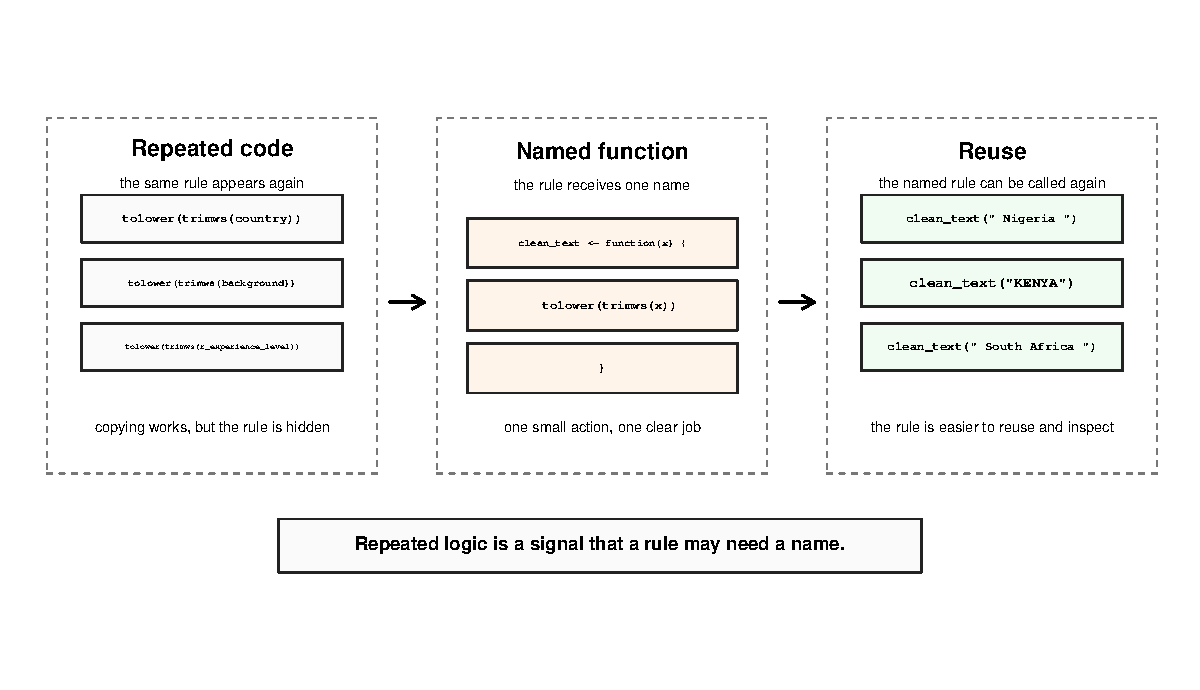
\includegraphics[width=0.9\linewidth,height=\textheight,keepaspectratio]{chapters/09-user-defined-functions_files/figure-pdf/fig-repetition-to-named-function-1.pdf}

}

\caption{\label{fig-repetition-to-named-function}From Repeated Code to a
Named Function}

\end{figure}%

As shown in Figure~\ref{fig-repetition-to-named-function}, the function
does not make the rule more mysterious. It makes the rule more visible.
The repeated pattern \texttt{tolower(trimws(...))} is now carried by the
name \texttt{clean\_text()}.

This is the heart of Chapter 9. A user-defined function is not mainly
about writing clever code. It is about preserving a small rule so it can
be reused, inspected, and trusted.

\section{Functions as Named Thinking}\label{functions-as-named-thinking}

A user-defined function is a function created by the user to perform a
reusable action.

That definition is accurate, but it is not yet the full mental model.

A beginner often thinks a function is mainly about writing shorter code.
Shorter code can be a benefit, but it is not the deepest reason
functions matter. A function is also a way of naming thinking.

This repeated line:

\begin{Shaded}
\begin{Highlighting}[]
\FunctionTok{tolower}\NormalTok{(}\FunctionTok{trimws}\NormalTok{(country))}
\end{Highlighting}
\end{Shaded}

contains a rule:

\begin{Shaded}
\begin{Highlighting}[]
\NormalTok{remove extra spaces, then convert text to lower case}
\end{Highlighting}
\end{Shaded}

When Leo turns that rule into a function, the code becomes easier to
read:

\begin{Shaded}
\begin{Highlighting}[]
\NormalTok{clean\_text }\OtherTok{\textless{}{-}} \ControlFlowTok{function}\NormalTok{(x) \{}
  \FunctionTok{tolower}\NormalTok{(}\FunctionTok{trimws}\NormalTok{(x))}
\NormalTok{\}}

\FunctionTok{clean\_text}\NormalTok{(}\StringTok{" Nigeria "}\NormalTok{)}
\CommentTok{\#\textgreater{} [1] "nigeria"}
\end{Highlighting}
\end{Shaded}

The function name \texttt{clean\_text} now carries meaning. In the same
way, a name like \texttt{completion\_rate()} or
\texttt{check\_high\_score()} tells the reader what analytical rule is
being applied. It tells the reader what the action is for.

This is the first major lesson of user-defined functions:

\begin{quote}
If a rule matters enough to repeat, it may matter enough to name.
\end{quote}

\section{Keep Beginner Functions
Small}\label{keep-beginner-functions-small}

At this stage, Leo should not try to turn every idea into a function.

A beginner function should usually do one clear thing: clean one kind of
text, calculate one ratio, check one condition, or repeat one small
rule. If a function becomes difficult to explain in one sentence, it may
be trying to do too much.

That boundary protects the learner.

A good beginner function can often be described like this:

\begin{Shaded}
\begin{Highlighting}[]
\NormalTok{This function cleans text.}
\NormalTok{This function adds a bonus.}
\NormalTok{This function calculates a completion rate.}
\NormalTok{This function checks whether a score is high enough.}
\end{Highlighting}
\end{Shaded}

A risky beginner function sounds like this:

\begin{Shaded}
\begin{Highlighting}[]
\NormalTok{This function cleans the data, fixes dates, removes duplicates,}
\NormalTok{calculates summaries, and prepares the final report.}
\end{Highlighting}
\end{Shaded}

That second idea may belong to a workflow later. It is too large for a
first user-defined function.

\begin{tcolorbox}[enhanced jigsaw, arc=.35mm, bottomrule=.15mm, breakable, colback=white, colframe=quarto-callout-warning-color-frame, left=2mm, leftrule=.75mm, opacityback=0, rightrule=.15mm, toprule=.15mm]
\begin{minipage}[t]{5.5mm}
\textcolor{quarto-callout-warning-color}{\faExclamationTriangle}
\end{minipage}%
\begin{minipage}[t]{\textwidth - 5.5mm}

\vspace{-3mm}\textbf{Beginner Boundary}\vspace{3mm}

A useful early function should be small enough to test with one or two
simple inputs.

\end{minipage}%
\end{tcolorbox}

\section{The Shape of a User-Defined
Function}\label{the-shape-of-a-user-defined-function}

A user-defined function has a recognisable shape:

\begin{Shaded}
\begin{Highlighting}[]
\NormalTok{name }\OtherTok{\textless{}{-}} \ControlFlowTok{function}\NormalTok{(input) \{}
\NormalTok{  action}
\NormalTok{\}}
\end{Highlighting}
\end{Shaded}

The shape has four parts:

\begin{Shaded}
\begin{Highlighting}[]
\NormalTok{name       = what Leo will call the action}
\NormalTok{input      = what the function receives}
\NormalTok{body       = what the function does}
\NormalTok{output     = what comes back}
\end{Highlighting}
\end{Shaded}

Here is a small function:

\begin{Shaded}
\begin{Highlighting}[]
\NormalTok{add\_bonus }\OtherTok{\textless{}{-}} \ControlFlowTok{function}\NormalTok{(score) \{}
\NormalTok{  score }\SpecialCharTok{+} \DecValTok{5}
\NormalTok{\}}
\end{Highlighting}
\end{Shaded}

The name is \texttt{add\_bonus}.

The input is \texttt{score}.

The body is:

\begin{Shaded}
\begin{Highlighting}[]
\NormalTok{score }\SpecialCharTok{+} \DecValTok{5}
\end{Highlighting}
\end{Shaded}

When the function is called, R runs the body using the value supplied
for \texttt{score}. The final evaluated result becomes the returned
output.

\begin{Shaded}
\begin{Highlighting}[]
\FunctionTok{add\_bonus}\NormalTok{(}\DecValTok{80}\NormalTok{)}
\CommentTok{\#\textgreater{} [1] 85}
\end{Highlighting}
\end{Shaded}

The input name inside the function does not need to match an existing
object outside the function. It is a temporary name R uses while the
function runs.

This function is small, but it teaches the structure. Leo has created an
action that R did not already have under that name.

\section{How R Thinks: Running a Function Leo
Created}\label{how-r-thinks-running-a-function-leo-created}

\begin{tcolorbox}[enhanced jigsaw, arc=.35mm, bottomrule=.15mm, breakable, colback=white, colframe=quarto-callout-tip-color-frame, left=2mm, leftrule=.75mm, opacityback=0, rightrule=.15mm, toprule=.15mm]
\begin{minipage}[t]{5.5mm}
\textcolor{quarto-callout-tip-color}{\faLightbulb}
\end{minipage}%
\begin{minipage}[t]{\textwidth - 5.5mm}

\vspace{-3mm}\textbf{How R Thinks}\vspace{3mm}

When Leo calls a user-defined function, R follows a simple path:

\begin{enumerate}
\def\labelenumi{\arabic{enumi}.}
\tightlist
\item
  R finds the function name.
\item
  R assigns the supplied value to the function input name.
\item
  R runs the code inside the function body.
\item
  R returns the final result.
\item
  Leo inspects the result before trusting it.
\end{enumerate}

\end{minipage}%
\end{tcolorbox}

For \texttt{add\_bonus(80)}, R sees the name \texttt{add\_bonus}, sends
\texttt{80} into the function as \texttt{score}, runs
\texttt{score\ +\ 5}, and returns \texttt{85}.

That is enough theory for now. Leo does not need scoping theory,
environments, or package-style function design in this chapter. He only
needs the working model:

\begin{Shaded}
\begin{Highlighting}[]
\NormalTok{input → named action → output}
\end{Highlighting}
\end{Shaded}

\section{Predict Before You Run}\label{predict-before-you-run-4}

Before running the next function call, Leo should pause.

\begin{Shaded}
\begin{Highlighting}[]
\NormalTok{add\_bonus }\OtherTok{\textless{}{-}} \ControlFlowTok{function}\NormalTok{(score) \{}
\NormalTok{  score }\SpecialCharTok{+} \DecValTok{5}
\NormalTok{\}}
\end{Highlighting}
\end{Shaded}

Predict the result of each line:

\begin{Shaded}
\begin{Highlighting}[]
\FunctionTok{add\_bonus}\NormalTok{(}\DecValTok{80}\NormalTok{)}
\FunctionTok{add\_bonus}\NormalTok{(}\DecValTok{72}\NormalTok{)}
\FunctionTok{add\_bonus}\NormalTok{(}\DecValTok{0}\NormalTok{)}
\end{Highlighting}
\end{Shaded}

Now run them.

\begin{Shaded}
\begin{Highlighting}[]
\FunctionTok{add\_bonus}\NormalTok{(}\DecValTok{80}\NormalTok{)}
\CommentTok{\#\textgreater{} [1] 85}
\FunctionTok{add\_bonus}\NormalTok{(}\DecValTok{72}\NormalTok{)}
\CommentTok{\#\textgreater{} [1] 77}
\FunctionTok{add\_bonus}\NormalTok{(}\DecValTok{0}\NormalTok{)}
\CommentTok{\#\textgreater{} [1] 5}
\end{Highlighting}
\end{Shaded}

The function applies the same rule each time. The input changes, but the
action remains stable.

That is the value of naming a repeated rule.

\section{Turning Repetition into a
Function}\label{turning-repetition-into-a-function}

Now return to the opening problem.

Leo had three separate text-cleaning lines:

\begin{Shaded}
\begin{Highlighting}[]
\NormalTok{country }\OtherTok{\textless{}{-}} \FunctionTok{tolower}\NormalTok{(}\FunctionTok{trimws}\NormalTok{(country))}
\NormalTok{background }\OtherTok{\textless{}{-}} \FunctionTok{tolower}\NormalTok{(}\FunctionTok{trimws}\NormalTok{(background))}
\NormalTok{r\_experience\_level }\OtherTok{\textless{}{-}} \FunctionTok{tolower}\NormalTok{(}\FunctionTok{trimws}\NormalTok{(r\_experience\_level))}
\end{Highlighting}
\end{Shaded}

The rule is repeated. The input changes.

That means the rule can be named:

\begin{Shaded}
\begin{Highlighting}[]
\NormalTok{clean\_text }\OtherTok{\textless{}{-}} \ControlFlowTok{function}\NormalTok{(x) \{}
  \FunctionTok{tolower}\NormalTok{(}\FunctionTok{trimws}\NormalTok{(x))}
\NormalTok{\}}
\end{Highlighting}
\end{Shaded}

Now the repeated code becomes easier to read:

\begin{Shaded}
\begin{Highlighting}[]
\NormalTok{country }\OtherTok{\textless{}{-}} \FunctionTok{clean\_text}\NormalTok{(country)}
\NormalTok{background }\OtherTok{\textless{}{-}} \FunctionTok{clean\_text}\NormalTok{(background)}
\NormalTok{r\_experience\_level }\OtherTok{\textless{}{-}} \FunctionTok{clean\_text}\NormalTok{(r\_experience\_level)}

\NormalTok{country}
\CommentTok{\#\textgreater{} [1] "nigeria"}
\NormalTok{background}
\CommentTok{\#\textgreater{} [1] "excel"}
\NormalTok{r\_experience\_level}
\CommentTok{\#\textgreater{} [1] "beginner"}
\end{Highlighting}
\end{Shaded}

The function does not make the rule more mysterious. It makes the rule
more visible.

A copied line remembers what Leo did once. A function preserves the
reasoning so the same rule can be reused consistently.

\begin{tcolorbox}[enhanced jigsaw, arc=.35mm, bottomrule=.15mm, breakable, colback=white, colframe=quarto-callout-important-color-frame, left=2mm, leftrule=.75mm, opacityback=0, rightrule=.15mm, toprule=.15mm]
\begin{minipage}[t]{5.5mm}
\textcolor{quarto-callout-important-color}{\faExclamation}
\end{minipage}%
\begin{minipage}[t]{\textwidth - 5.5mm}

\vspace{-3mm}\textbf{Reliable Analysis Rule}\vspace{3mm}

A function is not trustworthy because it exists. It becomes trustworthy
when its behaviour has been inspected.

\end{minipage}%
\end{tcolorbox}

\section{A Small Momentum Win}\label{a-small-momentum-win-1}

Here is the first visible payoff.

Leo can apply the same cleaning rule to different values without
rewriting the rule each time.

\begin{Shaded}
\begin{Highlighting}[]
\FunctionTok{clean\_text}\NormalTok{(}\StringTok{" Nigeria "}\NormalTok{)}
\CommentTok{\#\textgreater{} [1] "nigeria"}
\FunctionTok{clean\_text}\NormalTok{(}\StringTok{"KENYA"}\NormalTok{)}
\CommentTok{\#\textgreater{} [1] "kenya"}
\FunctionTok{clean\_text}\NormalTok{(}\StringTok{" South Africa "}\NormalTok{)}
\CommentTok{\#\textgreater{} [1] "south africa"}
\end{Highlighting}
\end{Shaded}

The action is consistent. The inputs vary.

That is a small win, but it is not a small idea. This is the beginning
of reusable workflow thinking.

The same principle can later help with variables from
\texttt{df\_r\_migration}, such as \texttt{country},
\texttt{background}, \texttt{completion\_status}, and
\texttt{r\_experience\_level}. This chapter does not need to load the
full dataset. The point is simpler: when the same text-standardising
rule appears again and again, Leo can give it one name.

\begin{Shaded}
\begin{Highlighting}[]
\NormalTok{df\_r\_migration}\SpecialCharTok{$}\NormalTok{country }\OtherTok{\textless{}{-}} \FunctionTok{clean\_text}\NormalTok{(df\_r\_migration}\SpecialCharTok{$}\NormalTok{country)}
\NormalTok{df\_r\_migration}\SpecialCharTok{$}\NormalTok{background }\OtherTok{\textless{}{-}} \FunctionTok{clean\_text}\NormalTok{(df\_r\_migration}\SpecialCharTok{$}\NormalTok{background)}
\NormalTok{df\_r\_migration}\SpecialCharTok{$}\NormalTok{completion\_status }\OtherTok{\textless{}{-}} \FunctionTok{clean\_text}\NormalTok{(df\_r\_migration}\SpecialCharTok{$}\NormalTok{completion\_status)}
\NormalTok{df\_r\_migration}\SpecialCharTok{$}\NormalTok{r\_experience\_level }\OtherTok{\textless{}{-}} \FunctionTok{clean\_text}\NormalTok{(df\_r\_migration}\SpecialCharTok{$}\NormalTok{r\_experience\_level)}
\end{Highlighting}
\end{Shaded}

The full cleaning workflow belongs later. For now, Leo is learning why a
repeated rule should not be scattered across a script.

\section{Inputs, Body, and Output}\label{inputs-body-and-output}

A user-defined function becomes easier to understand when Leo separates
three questions.

\begin{Shaded}
\begin{Highlighting}[]
\NormalTok{What does the function receive?}
\NormalTok{What does the function do?}
\NormalTok{What does the function return?}
\end{Highlighting}
\end{Shaded}

Take this function:

\begin{Shaded}
\begin{Highlighting}[]
\NormalTok{completion\_rate }\OtherTok{\textless{}{-}} \ControlFlowTok{function}\NormalTok{(completed) \{}
  \FunctionTok{mean}\NormalTok{(completed, }\AttributeTok{na.rm =} \ConstantTok{TRUE}\NormalTok{)}
\NormalTok{\}}
\end{Highlighting}
\end{Shaded}

The input is \texttt{completed}.

The body calculates the mean of the logical values.

The output is a completion rate.

\begin{Shaded}
\begin{Highlighting}[]
\NormalTok{completion\_status }\OtherTok{\textless{}{-}} \FunctionTok{c}\NormalTok{(}\ConstantTok{TRUE}\NormalTok{, }\ConstantTok{TRUE}\NormalTok{, }\ConstantTok{FALSE}\NormalTok{, }\ConstantTok{TRUE}\NormalTok{, }\ConstantTok{NA}\NormalTok{)}

\FunctionTok{completion\_rate}\NormalTok{(completion\_status)}
\CommentTok{\#\textgreater{} [1] 0.75}
\end{Highlighting}
\end{Shaded}

In R, \texttt{TRUE} behaves like \texttt{1} and \texttt{FALSE} behaves
like \texttt{0} in this kind of calculation. The function uses
\texttt{na.rm\ =\ TRUE} so that a missing value does not block the
result.

This function is still beginner-sized. It does one clear thing.

\section{Predict Before You Run: Text
Cleaning}\label{predict-before-you-run-text-cleaning}

Before running the next call, predict what will happen.

\begin{Shaded}
\begin{Highlighting}[]
\NormalTok{clean\_country }\OtherTok{\textless{}{-}} \ControlFlowTok{function}\NormalTok{(country) \{}
  \FunctionTok{tolower}\NormalTok{(}\FunctionTok{trimws}\NormalTok{(country))}
\NormalTok{\}}
\end{Highlighting}
\end{Shaded}

What will this return?

\begin{Shaded}
\begin{Highlighting}[]
\FunctionTok{clean\_country}\NormalTok{(}\StringTok{" Nigeria "}\NormalTok{)}
\end{Highlighting}
\end{Shaded}

Run it.

\begin{Shaded}
\begin{Highlighting}[]
\FunctionTok{clean\_country}\NormalTok{(}\StringTok{" Nigeria "}\NormalTok{)}
\CommentTok{\#\textgreater{} [1] "nigeria"}
\end{Highlighting}
\end{Shaded}

The leading and trailing spaces disappear, and the text becomes lower
case.

Now test a few more inputs.

\begin{Shaded}
\begin{Highlighting}[]
\FunctionTok{clean\_country}\NormalTok{(}\StringTok{"KENYA"}\NormalTok{)}
\CommentTok{\#\textgreater{} [1] "kenya"}
\FunctionTok{clean\_country}\NormalTok{(}\StringTok{" south africa "}\NormalTok{)}
\CommentTok{\#\textgreater{} [1] "south africa"}
\FunctionTok{clean\_country}\NormalTok{(}\ConstantTok{NA}\NormalTok{)}
\CommentTok{\#\textgreater{} [1] NA}
\end{Highlighting}
\end{Shaded}

The \texttt{NA} remains \texttt{NA}. That is useful. The function does
not pretend that a missing value is real text.

This is another inspection habit: do not only test the clean-looking
case. Test the edge case that may appear in real data.

\section{Testing a Function Before Trusting
It}\label{testing-a-function-before-trusting-it}

A function should be tested before it becomes part of a workflow.

Testing does not have to be advanced at this stage. Leo can begin with a
simple checklist:

\begin{Shaded}
\begin{Highlighting}[]
\NormalTok{Does the function work on a normal input?}
\NormalTok{Does it work on a second normal input?}
\NormalTok{Does it behave sensibly with missing input?}
\NormalTok{Does the output look like the kind of result I expected?}
\end{Highlighting}
\end{Shaded}

For \texttt{clean\_text()}, the tests are simple:

\begin{Shaded}
\begin{Highlighting}[]
\FunctionTok{clean\_text}\NormalTok{(}\StringTok{" Nigeria "}\NormalTok{)}
\CommentTok{\#\textgreater{} [1] "nigeria"}
\FunctionTok{clean\_text}\NormalTok{(}\StringTok{"KENYA"}\NormalTok{)}
\CommentTok{\#\textgreater{} [1] "kenya"}
\FunctionTok{clean\_text}\NormalTok{(}\StringTok{" South Africa "}\NormalTok{)}
\CommentTok{\#\textgreater{} [1] "south africa"}
\FunctionTok{clean\_text}\NormalTok{(}\ConstantTok{NA}\NormalTok{)}
\CommentTok{\#\textgreater{} [1] NA}
\end{Highlighting}
\end{Shaded}

For \texttt{add\_bonus()}, the tests are also simple:

\begin{Shaded}
\begin{Highlighting}[]
\FunctionTok{add\_bonus}\NormalTok{(}\DecValTok{80}\NormalTok{)}
\CommentTok{\#\textgreater{} [1] 85}
\FunctionTok{add\_bonus}\NormalTok{(}\DecValTok{0}\NormalTok{)}
\CommentTok{\#\textgreater{} [1] 5}
\FunctionTok{add\_bonus}\NormalTok{(}\SpecialCharTok{{-}}\DecValTok{5}\NormalTok{)}
\CommentTok{\#\textgreater{} [1] 0}
\end{Highlighting}
\end{Shaded}

The last input is not a recommendation about negative scores. It is a
reminder that tests help Leo notice assumptions. If a negative score
should not be allowed, that becomes a design decision. It should not be
hidden.

\begin{tcolorbox}[enhanced jigsaw, arc=.35mm, bottomrule=.15mm, breakable, colback=white, colframe=quarto-callout-note-color-frame, left=2mm, leftrule=.75mm, opacityback=0, rightrule=.15mm, toprule=.15mm]
\begin{minipage}[t]{5.5mm}
\textcolor{quarto-callout-note-color}{\faInfo}
\end{minipage}%
\begin{minipage}[t]{\textwidth - 5.5mm}

\vspace{-3mm}\textbf{Inspection Before Trust}\vspace{3mm}

Calling a function is not the end of the work. A reliable analyst checks
what came back.

\end{minipage}%
\end{tcolorbox}

\section{Simple Input Checks}\label{simple-input-checks}

Some functions need a small guardrail.

Suppose Leo wants a function that calculates an average score, but only
when the input is numeric. A simple check can make the function safer.

\begin{Shaded}
\begin{Highlighting}[]
\NormalTok{safe\_mean }\OtherTok{\textless{}{-}} \ControlFlowTok{function}\NormalTok{(x) \{}
  \ControlFlowTok{if}\NormalTok{ (}\SpecialCharTok{!}\FunctionTok{is.numeric}\NormalTok{(x)) \{}
    \FunctionTok{stop}\NormalTok{(}\StringTok{"safe\_mean() expects numeric input."}\NormalTok{)}
\NormalTok{  \}}

  \FunctionTok{mean}\NormalTok{(x, }\AttributeTok{na.rm =} \ConstantTok{TRUE}\NormalTok{)}
\NormalTok{\}}
\end{Highlighting}
\end{Shaded}

Now the normal case works:

\begin{Shaded}
\begin{Highlighting}[]
\FunctionTok{safe\_mean}\NormalTok{(}\FunctionTok{c}\NormalTok{(}\DecValTok{72}\NormalTok{, }\DecValTok{81}\NormalTok{, }\ConstantTok{NA}\NormalTok{, }\DecValTok{90}\NormalTok{))}
\CommentTok{\#\textgreater{} [1] 81}
\end{Highlighting}
\end{Shaded}

The function says its expectation clearly: the input should be numeric.

A non-numeric example should not be run accidentally in a rendered
chapter unless it is marked as an intentional error. So here is the idea
as display-only code:

\begin{Shaded}
\begin{Highlighting}[]
\FunctionTok{safe\_mean}\NormalTok{(}\FunctionTok{c}\NormalTok{(}\StringTok{"72"}\NormalTok{, }\StringTok{"81"}\NormalTok{, }\StringTok{"90"}\NormalTok{))}
\CommentTok{\# Error: safe\_mean() expects numeric input.}
\end{Highlighting}
\end{Shaded}

The input check is simple. The error is intentional because the function
is protecting the workflow from the wrong kind of input. It does not
turn Leo into a software engineer. It only makes the function honest
about what it expects.

Use checks sparingly at this stage. A function with too many checks can
become harder to read than the problem it was meant to solve.

\section{The New Responsibility: When Leo Names an
Action}\label{the-new-responsibility-when-leo-names-an-action}

User-defined functions give Leo more control, but they also give him
more responsibility.

When Leo uses \texttt{mean()} incorrectly, the problem belongs to how he
called a function R already knows. When he writes \texttt{safe\_mean()}
himself, the question becomes wider:

\begin{Shaded}
\begin{Highlighting}[]
\NormalTok{Did I give the function the right input?}
\NormalTok{Did I name the argument clearly?}
\NormalTok{Did I assume the input would always be numeric?}
\NormalTok{Did I test the unusual case?}
\NormalTok{Did the function fail because of the call, or because of the function body?}
\end{Highlighting}
\end{Shaded}

This is not a reason to avoid user-defined functions. It is the reason
to write them carefully.

A function is useful because it hides repeated detail behind a name. But
if Leo hides too much too early, he may also hide the source of a
problem. That is why small functions are easier to test, easier to
explain, and easier to repair.

\begin{tcolorbox}[enhanced jigsaw, arc=.35mm, bottomrule=.15mm, breakable, colback=white, colframe=quarto-callout-tip-color-frame, left=2mm, leftrule=.75mm, opacityback=0, rightrule=.15mm, toprule=.15mm]
\begin{minipage}[t]{5.5mm}
\textcolor{quarto-callout-tip-color}{\faLightbulb}
\end{minipage}%
\begin{minipage}[t]{\textwidth - 5.5mm}

\vspace{-3mm}\textbf{Bridge to Debugging}\vspace{3mm}

A function names a repeated action. Debugging asks what happened when
that named action did not behave as expected.

\end{minipage}%
\end{tcolorbox}

\section{When a Function Is Trying to Do Too
Much}\label{when-a-function-is-trying-to-do-too-much}

A common beginner mistake is to create one large function that tries to
solve an entire project.

That usually happens for a reasonable reason. Leo wants the script to
feel tidy. He thinks putting many lines into one function will make the
work cleaner.

But a function that does too many things becomes difficult to inspect.

Consider this display-only sketch:

\begin{Shaded}
\begin{Highlighting}[]
\NormalTok{prepare\_everything }\OtherTok{\textless{}{-}} \ControlFlowTok{function}\NormalTok{(data) \{}
  \CommentTok{\# clean text}
  \CommentTok{\# fix dates}
  \CommentTok{\# remove duplicates}
  \CommentTok{\# calculate new variables}
  \CommentTok{\# summarise results}
  \CommentTok{\# export report}
\NormalTok{\}}
\end{Highlighting}
\end{Shaded}

The name is vague, and the responsibilities are too many.

A better beginner habit is to name one small rule at a time:

\begin{Shaded}
\begin{Highlighting}[]
\FunctionTok{clean\_text}\NormalTok{()}
\FunctionTok{calculate\_completion\_rate}\NormalTok{()}
\FunctionTok{check\_high\_score}\NormalTok{()}
\end{Highlighting}
\end{Shaded}

Small functions are easier to test. They are also easier to replace when
the rule changes.

The point is not to write many functions for the sake of writing
functions. The point is to name repeated reasoning clearly.

\section{A Small Repair Moment}\label{a-small-repair-moment}

Leo first writes this:

\begin{Shaded}
\begin{Highlighting}[]
\NormalTok{clean\_learner\_record }\OtherTok{\textless{}{-}} \ControlFlowTok{function}\NormalTok{(country, background, r\_experience\_level) \{}
\NormalTok{  country }\OtherTok{\textless{}{-}} \FunctionTok{tolower}\NormalTok{(}\FunctionTok{trimws}\NormalTok{(country))}
\NormalTok{  background }\OtherTok{\textless{}{-}} \FunctionTok{tolower}\NormalTok{(}\FunctionTok{trimws}\NormalTok{(background))}
\NormalTok{  r\_experience\_level }\OtherTok{\textless{}{-}} \FunctionTok{tolower}\NormalTok{(}\FunctionTok{trimws}\NormalTok{(r\_experience\_level))}

  \FunctionTok{list}\NormalTok{(country, background, r\_experience\_level)}
\NormalTok{\}}
\end{Highlighting}
\end{Shaded}

The function works, but it is already doing several things at once. It
cleans three inputs and then pastes them together. That may be more than
Leo needs.

He steps back and asks a better question:

\begin{quote}
What is the repeated rule?
\end{quote}

The repeated rule is not ``prepare a learner record.'' It is:

\begin{Shaded}
\begin{Highlighting}[]
\NormalTok{standardise one piece of text}
\end{Highlighting}
\end{Shaded}

So he keeps the smaller function:

\begin{Shaded}
\begin{Highlighting}[]
\NormalTok{standardise\_text }\OtherTok{\textless{}{-}} \ControlFlowTok{function}\NormalTok{(x) \{}
  \FunctionTok{tolower}\NormalTok{(}\FunctionTok{trimws}\NormalTok{(x))}
\NormalTok{\}}

\FunctionTok{standardise\_text}\NormalTok{(}\StringTok{" Beginner "}\NormalTok{)}
\CommentTok{\#\textgreater{} [1] "beginner"}
\end{Highlighting}
\end{Shaded}

That is the repair. Leo has not failed. He has made the function smaller
until its purpose is clear.

\section{Default Arguments}\label{default-arguments}

Some functions need a setting that has a common value but can still be
changed.

A default argument gives the function a normal setting.

\begin{Shaded}
\begin{Highlighting}[]
\NormalTok{add\_bonus }\OtherTok{\textless{}{-}} \ControlFlowTok{function}\NormalTok{(score, }\AttributeTok{bonus =} \DecValTok{5}\NormalTok{) \{}
\NormalTok{  score }\SpecialCharTok{+}\NormalTok{ bonus}
\NormalTok{\}}
\end{Highlighting}
\end{Shaded}

Now Leo can omit the second argument and use the default:

\begin{Shaded}
\begin{Highlighting}[]
\FunctionTok{add\_bonus}\NormalTok{(}\DecValTok{80}\NormalTok{)}
\CommentTok{\#\textgreater{} [1] 85}
\end{Highlighting}
\end{Shaded}

Or he can choose a different bonus:

\begin{Shaded}
\begin{Highlighting}[]
\FunctionTok{add\_bonus}\NormalTok{(}\DecValTok{80}\NormalTok{, }\AttributeTok{bonus =} \DecValTok{10}\NormalTok{)}
\CommentTok{\#\textgreater{} [1] 90}
\end{Highlighting}
\end{Shaded}

The default should match the usual case. The named argument makes the
unusual case clear.

This is another place where functions protect meaning. The code says
what changed.

\section{Naming Functions Clearly}\label{naming-functions-clearly}

A function name should help the reader understand the action.

These names are helpful:

\begin{Shaded}
\begin{Highlighting}[]
\FunctionTok{clean\_text}\NormalTok{()}
\FunctionTok{add\_bonus}\NormalTok{()}
\FunctionTok{completion\_rate}\NormalTok{()}
\FunctionTok{safe\_mean}\NormalTok{()}
\end{Highlighting}
\end{Shaded}

These names are weak:

\begin{Shaded}
\begin{Highlighting}[]
\FunctionTok{do\_it}\NormalTok{()}
\FunctionTok{fix\_stuff}\NormalTok{()}
\FunctionTok{my\_function}\NormalTok{()}
\FunctionTok{thing}\NormalTok{()}
\end{Highlighting}
\end{Shaded}

A good function name is not decorative. It is part of the explanation.

When Leo reads \texttt{completion\_rate(completion\_status)}, he can
infer the intention before he studies the body. That is what clear names
do.

\section{Common Beginner Mistakes}\label{common-beginner-mistakes-2}

\subsection{Mistake 1: Defining a Function but Forgetting to Call
It}\label{mistake-1-defining-a-function-but-forgetting-to-call-it}

This defines a function:

\begin{Shaded}
\begin{Highlighting}[]
\NormalTok{double\_score }\OtherTok{\textless{}{-}} \ControlFlowTok{function}\NormalTok{(score) \{}
\NormalTok{  score }\SpecialCharTok{*} \DecValTok{2}
\NormalTok{\}}
\end{Highlighting}
\end{Shaded}

But nothing has happened to a real score yet.

To use the function, Leo must call it:

\begin{Shaded}
\begin{Highlighting}[]
\FunctionTok{double\_score}\NormalTok{(}\DecValTok{40}\NormalTok{)}
\CommentTok{\#\textgreater{} [1] 80}
\end{Highlighting}
\end{Shaded}

Defining is not the same as running.

\subsection{Mistake 2: Using an Outside Object by
Accident}\label{mistake-2-using-an-outside-object-by-accident}

This function depends on an object outside the function:

\begin{Shaded}
\begin{Highlighting}[]
\NormalTok{bonus }\OtherTok{\textless{}{-}} \DecValTok{5}

\NormalTok{add\_bonus\_badly }\OtherTok{\textless{}{-}} \ControlFlowTok{function}\NormalTok{(score) \{}
\NormalTok{  score }\SpecialCharTok{+}\NormalTok{ bonus}
\NormalTok{\}}
\end{Highlighting}
\end{Shaded}

It may work while \texttt{bonus} exists. But the function is less clear
because the input is not fully visible.

A clearer version receives the bonus directly:

\begin{Shaded}
\begin{Highlighting}[]
\NormalTok{add\_bonus\_clearly }\OtherTok{\textless{}{-}} \ControlFlowTok{function}\NormalTok{(score, }\AttributeTok{bonus =} \DecValTok{5}\NormalTok{) \{}
\NormalTok{  score }\SpecialCharTok{+}\NormalTok{ bonus}
\NormalTok{\}}

\FunctionTok{add\_bonus\_clearly}\NormalTok{(}\DecValTok{80}\NormalTok{)}
\CommentTok{\#\textgreater{} [1] 85}
\end{Highlighting}
\end{Shaded}

This is not a full lesson on environments. It is a beginner rule of
clarity: important inputs should usually be visible in the function
definition.

\subsection{Mistake 3: Making the Function Too
Big}\label{mistake-3-making-the-function-too-big}

A function that cleans text, calculates rates, creates summaries, and
exports a file is probably too large for this stage.

A beginner function should usually do one clear thing. If the purpose
cannot be explained in one sentence, split the idea.

\subsection{Mistake 4: Forgetting to Inspect the
Output}\label{mistake-4-forgetting-to-inspect-the-output}

A function can return a result that looks plausible but is not what Leo
intended.

So Leo should test small cases first:

\begin{Shaded}
\begin{Highlighting}[]
\FunctionTok{completion\_rate}\NormalTok{(}\FunctionTok{c}\NormalTok{(}\ConstantTok{TRUE}\NormalTok{, }\ConstantTok{FALSE}\NormalTok{, }\ConstantTok{TRUE}\NormalTok{))}
\CommentTok{\#\textgreater{} [1] 0.6666667}
\FunctionTok{completion\_rate}\NormalTok{(}\FunctionTok{c}\NormalTok{(}\ConstantTok{TRUE}\NormalTok{, }\ConstantTok{NA}\NormalTok{, }\ConstantTok{TRUE}\NormalTok{))}
\CommentTok{\#\textgreater{} [1] 1}
\end{Highlighting}
\end{Shaded}

A function is part of analysis only after its behaviour has been
checked.

\section{What Leo Is Expected to Know at This
Point}\label{what-leo-is-expected-to-know-at-this-point-4}

At this point, Leo is not expected to design software systems or write
complex function libraries.

He is expected to understand that:

\begin{itemize}
\tightlist
\item
  repeated code can signal repeated logic;
\item
  a repeated rule can be given a name;
\item
  a user-defined function has a name, input, body, and output;
\item
  beginner functions should stay small;
\item
  functions should be tested with simple inputs;
\item
  clear function names make workflows easier to read.
\end{itemize}

\begin{tcolorbox}[enhanced jigsaw, arc=.35mm, bottomrule=.15mm, breakable, colback=white, colframe=quarto-callout-note-color-frame, left=2mm, leftrule=.75mm, opacityback=0, rightrule=.15mm, toprule=.15mm]
\begin{minipage}[t]{5.5mm}
\textcolor{quarto-callout-note-color}{\faInfo}
\end{minipage}%
\begin{minipage}[t]{\textwidth - 5.5mm}

\vspace{-3mm}\textbf{Not Yet}\vspace{3mm}

Leo is not expected to understand advanced scoping, package development,
recursive functions, object-oriented programming, formal testing
frameworks, or functional programming tools. Those belong later.

He is also not expected to diagnose every error message in this chapter.
For now, the goal is small, readable functions that preserve repeated
reasoning and can be tested before they are trusted. Chapter 10 will
turn that testing habit into a fuller debugging framework.

\end{minipage}%
\end{tcolorbox}

\section{A Small Practice Lab}\label{a-small-practice-lab-1}

\subsection{Task 1: Predict the Output}\label{task-1-predict-the-output}

Before running the code, predict the result.

\begin{Shaded}
\begin{Highlighting}[]
\NormalTok{completion\_rate }\OtherTok{\textless{}{-}} \ControlFlowTok{function}\NormalTok{(completed) \{}
  \FunctionTok{mean}\NormalTok{(completed, }\AttributeTok{na.rm =} \ConstantTok{TRUE}\NormalTok{)}
\NormalTok{\}}

\FunctionTok{completion\_rate}\NormalTok{(}\FunctionTok{c}\NormalTok{(}\ConstantTok{TRUE}\NormalTok{, }\ConstantTok{TRUE}\NormalTok{, }\ConstantTok{FALSE}\NormalTok{, }\ConstantTok{NA}\NormalTok{))}
\CommentTok{\#\textgreater{} [1] 0.6666667}
\end{Highlighting}
\end{Shaded}

Now explain the result in one sentence.

\subsection{Task 2: Name the Repeated
Rule}\label{task-2-name-the-repeated-rule}

Look at the repeated pattern:

\begin{Shaded}
\begin{Highlighting}[]
\FunctionTok{tolower}\NormalTok{(}\FunctionTok{trimws}\NormalTok{(}\StringTok{" Nigeria "}\NormalTok{))}
\FunctionTok{tolower}\NormalTok{(}\FunctionTok{trimws}\NormalTok{(}\StringTok{"KENYA"}\NormalTok{))}
\FunctionTok{tolower}\NormalTok{(}\FunctionTok{trimws}\NormalTok{(}\StringTok{" South Africa "}\NormalTok{))}
\end{Highlighting}
\end{Shaded}

Write a function called \texttt{clean\_text()} that names the rule.

\subsection{Task 3: Test Before Trust}\label{task-3-test-before-trust}

After writing \texttt{clean\_text()}, test it with:

\begin{Shaded}
\begin{Highlighting}[]
\FunctionTok{clean\_text}\NormalTok{(}\StringTok{" Nigeria "}\NormalTok{)}
\FunctionTok{clean\_text}\NormalTok{(}\StringTok{"KENYA"}\NormalTok{)}
\FunctionTok{clean\_text}\NormalTok{(}\ConstantTok{NA}\NormalTok{)}
\end{Highlighting}
\end{Shaded}

Write down what each result tells you.

\subsection{Task 4: Keep It Small}\label{task-4-keep-it-small}

Explain why this is too much for one beginner function:

\begin{Shaded}
\begin{Highlighting}[]
\NormalTok{prepare\_report }\OtherTok{\textless{}{-}} \ControlFlowTok{function}\NormalTok{(data) \{}
  \CommentTok{\# import data}
  \CommentTok{\# clean text}
  \CommentTok{\# fix dates}
  \CommentTok{\# remove duplicates}
  \CommentTok{\# summarise results}
  \CommentTok{\# make charts}
\NormalTok{\}}
\end{Highlighting}
\end{Shaded}

Then write one smaller function name that would be easier to test.

\section{Chapter Outcome}\label{chapter-outcome-8}

By the end of this chapter, Leo should be able to:

\begin{itemize}
\tightlist
\item
  recognise repeated code as a signal that a rule may need a name;
\item
  write a small user-defined function;
\item
  identify a function's name, input, body, and output;
\item
  call a function with different inputs;
\item
  use a simple default argument;
\item
  add a simple input check when needed;
\item
  test a function before trusting it;
\item
  explain why small functions are easier to inspect and repair;
\item
  understand why user-defined functions lead naturally into debugging.
\end{itemize}

These are not software-engineering skills in disguise. They are
practical analysis skills. Leo is learning to keep repeated reasoning in
one place, give it a meaningful name, and check whether it behaves as
expected.

\section{From Naming Actions to Checking
Behaviour}\label{from-naming-actions-to-checking-behaviour}

Part 2 has not finished yet, but Leo has reached an important threshold.

Chapter 6 showed him that R code has structure. Code is not a pile of
symbols. It must be arranged in ways R can read.

Chapter 7 showed him that R can make judgments. Comparisons, logical
values, and conditions allow code to ask careful questions.

Chapter 8 showed him that R already knows many actions. Built-in
functions gave Leo a vocabulary of named work: inspect, count,
summarise, convert, check, format, and clean.

Chapter 9 has added one more layer. Leo can now create small named
actions of his own.

The movement now looks like this:

\begin{Shaded}
\begin{Highlighting}[]
\NormalTok{Chapter 6: R reads structured code.}
\NormalTok{Chapter 7: R makes and combines judgments.}
\NormalTok{Chapter 8: R performs ready{-}made actions.}
\NormalTok{Chapter 9: Leo creates small named actions of his own.}
\NormalTok{Chapter 10: Leo learns how to diagnose what went wrong.}
\end{Highlighting}
\end{Shaded}

That final line matters. A user-defined function gives Leo more power,
but it also gives him more responsibility. When a function fails, he can
no longer treat the problem as a mysterious event outside his control.
He must learn how to read what R says, trace where the problem began,
and test the assumptions hidden inside the code.

This is not a new topic dropped into the book. It is the natural
consequence of writing code that belongs to Leo.

\begin{tcolorbox}[enhanced jigsaw, arc=.35mm, bottomrule=.15mm, breakable, colback=white, colframe=quarto-callout-important-color-frame, left=2mm, leftrule=.75mm, opacityback=0, rightrule=.15mm, toprule=.15mm]
\begin{minipage}[t]{5.5mm}
\textcolor{quarto-callout-important-color}{\faExclamation}
\end{minipage}%
\begin{minipage}[t]{\textwidth - 5.5mm}

\vspace{-3mm}\textbf{Reliable Function Habit}\vspace{3mm}

A function is not reliable because it has a name. It becomes reliable
when Leo can explain its input, inspect its output, and test what
happens when the input is not quite what he expected.

\end{minipage}%
\end{tcolorbox}

\section{What Comes Next}\label{what-comes-next-2}

Leo has learned to name repeated thinking.

That changes his relationship with R. He is no longer only calling
actions that already exist. He is beginning to create actions that carry
his own assumptions.

This is powerful, but it also raises a new question:

\begin{quote}
What should Leo do when the code he wrote does not behave the way he
expected?
\end{quote}

That question belongs to Chapter 10.

The next chapter teaches Leo how to read errors without panic, trace
problems carefully, test small pieces of code, and repair the
conversation between his intention and R's response. Only after that
final Part 2 skill will he be ready to move into the larger workflows of
Part 3.

\chapter{Debugging R: A Practical Framework for Reading and Fixing
Errors}\label{debugging-r-a-practical-framework-for-reading-and-fixing-errors}

\renewcommand{\thefigure}{10.\arabic{figure}}
\setcounter{figure}{0}
\renewcommand{\thetable}{10.\arabic{table}}
\setcounter{table}{0}

\section{Opening Scene: When Working Code Stops
Working}\label{opening-scene-when-working-code-stops-working}

Leo has just learned something powerful.

He no longer has to repeat the same action again and again. If a rule
matters, he can give it a name. If a cleaning step appears in several
places, he can wrap it inside a function. If a calculation keeps
returning to the script, he can turn it into a reusable action.

That feels like progress.

Then he writes this:

\begin{Shaded}
\begin{Highlighting}[]
\NormalTok{clean\_text }\OtherTok{\textless{}{-}} \ControlFlowTok{function}\NormalTok{(value) \{}
  \FunctionTok{tolower}\NormalTok{(}\FunctionTok{trimws}\NormalTok{(value))}
\NormalTok{\}}

\FunctionTok{clean\_text}\NormalTok{(}\StringTok{" Nigeria "}\NormalTok{)}
\end{Highlighting}
\end{Shaded}

The code works.

So he becomes bolder.

\begin{Shaded}
\begin{Highlighting}[]
\NormalTok{clean\_text }\OtherTok{\textless{}{-}} \ControlFlowTok{function}\NormalTok{(value) \{}
  \FunctionTok{tolower}\NormalTok{(}\FunctionTok{trimws}\NormalTok{(value))}
\NormalTok{\}}

\NormalTok{country }\OtherTok{\textless{}{-}} \FunctionTok{clean\_text}\NormalTok{(}\StringTok{" Nigeria "}\NormalTok{)}
\NormalTok{background }\OtherTok{\textless{}{-}} \FunctionTok{clean\_text}\NormalTok{(}\StringTok{" Excel "}\NormalTok{)}
\NormalTok{r\_experience\_level }\OtherTok{\textless{}{-}} \FunctionTok{clean\_text}\NormalTok{(beginner)}
\end{Highlighting}
\end{Shaded}

Then R answers:

\begin{Shaded}
\begin{Highlighting}[]
\NormalTok{Error: object \textquotesingle{}beginner\textquotesingle{} not found}
\end{Highlighting}
\end{Shaded}

Leo stares at the screen.

The function worked before. The idea is correct. The code even looks
familiar. But R has stopped.

This is the point where many beginners feel that R has become hostile.
It has not. R is doing something more precise than that. It is telling
Leo that the conversation broke at a specific place.

R was not given the text \texttt{"beginner"}. It was given a name,
\texttt{beginner}, and no object with that name exists.

The problem is not that Leo is bad at R. The problem is that R received
something different from what Leo intended.

That difference is where debugging begins.

Chapter 10 starts from a practical truth every serious R learner must
eventually accept:

\begin{quote}
Code that breaks is not failed learning. It is information waiting to be
interpreted.
\end{quote}

\begin{tcolorbox}[enhanced jigsaw, arc=.35mm, bottomrule=.15mm, breakable, colback=white, colframe=quarto-callout-note-color-frame, left=2mm, leftrule=.75mm, opacityback=0, rightrule=.15mm, toprule=.15mm]
\begin{minipage}[t]{5.5mm}
\textcolor{quarto-callout-note-color}{\faInfo}
\end{minipage}%
\begin{minipage}[t]{\textwidth - 5.5mm}

\vspace{-3mm}\textbf{Chapter Compass}\vspace{3mm}

In this chapter, Leo learns how to read R errors calmly, distinguish
errors from warnings and messages, diagnose common beginner problems,
test code in smaller pieces, debug pipes and user-defined functions, and
close Part 2 with a practical framework for repairing code when the
conversation with R breaks down.

\end{minipage}%
\end{tcolorbox}

\section{What Changed After Chapter
9}\label{what-changed-after-chapter-9}

Chapter 9 changed Leo's relationship with R.

Before Chapter 9, functions were mostly tools other people had already
written. Leo used \texttt{mean()}, \texttt{length()}, \texttt{str()},
\texttt{tolower()}, and \texttt{trimws()} as ready-made actions. After
Chapter 9, he learned that he could name actions of his own.

That is a major step.

A user-defined function is more than a convenience. It is a sign that
Leo is beginning to think like an analyst who wants reusable logic, not
scattered repetition.

But reusable logic creates a new responsibility.

If a repeated line of code contains a problem, the problem may appear
once. If a function contains a problem, the problem can travel
everywhere the function is used. That is not a reason to fear functions.
It is a reason to learn how to diagnose them.

Part 2 has taught Leo the language of R: values, types, structures,
syntax, logic, operators, built-in functions, and user-defined
functions. Chapter 10 adds the missing skill that makes the language
usable in real life.

Leo must learn what to do when R answers back with an error.

\section{The Lightbulb: Errors Are
Signals}\label{the-lightbulb-errors-are-signals}

An error message is not R refusing to help.

It is R telling Leo where the conversation broke down.

That sentence matters because it changes the emotional posture of
debugging. When Leo sees an error, the first task is not to blame
himself, blame R, or paste the whole script into a search engine. The
first task is to ask a smaller, calmer question:

\begin{quote}
What did R receive, and what did R expect?
\end{quote}

Most beginner errors come from a mismatch between intention and
instruction.

Leo intended to give R a text value, but wrote an unquoted object name.
He intended to call a function, but misspelled it. He intended to use a
column, but the column name was different from what he remembered. He
intended to calculate with numbers, but one value was stored as text. He
intended to use a package function, but the package had not been loaded.

Debugging is the work of finding that mismatch.

\begin{tcolorbox}[enhanced jigsaw, arc=.35mm, bottomrule=.15mm, breakable, colback=white, colframe=quarto-callout-important-color-frame, left=2mm, leftrule=.75mm, opacityback=0, rightrule=.15mm, toprule=.15mm]
\begin{minipage}[t]{5.5mm}
\textcolor{quarto-callout-important-color}{\faExclamation}
\end{minipage}%
\begin{minipage}[t]{\textwidth - 5.5mm}

\vspace{-3mm}\textbf{Reliable Workflow Rule}\vspace{3mm}

Do not treat an error as a verdict. Treat it as a clue. The question is
not ``Why is R doing this to me?'' The better question is ``What exactly
did R receive, and where did that differ from what I intended?''

\end{minipage}%
\end{tcolorbox}

\section{Errors, Warnings, and Messages Are Not the
Same}\label{errors-warnings-and-messages-are-not-the-same}

R does not communicate problems in only one way.

Sometimes R stops. Sometimes it continues but warns Leo. Sometimes it
simply provides information about what happened. These signals are
related, but they are not identical.

\begin{longtable}[]{@{}
  >{\raggedright\arraybackslash}p{(\linewidth - 6\tabcolsep) * \real{0.2500}}
  >{\raggedright\arraybackslash}p{(\linewidth - 6\tabcolsep) * \real{0.2500}}
  >{\raggedright\arraybackslash}p{(\linewidth - 6\tabcolsep) * \real{0.2500}}
  >{\raggedright\arraybackslash}p{(\linewidth - 6\tabcolsep) * \real{0.2500}}@{}}
\caption{Errors, Warnings, and Messages in
R}\label{tbl-signals}\tabularnewline
\toprule\noalign{}
\begin{minipage}[b]{\linewidth}\raggedright
Signal
\end{minipage} & \begin{minipage}[b]{\linewidth}\raggedright
What it means
\end{minipage} & \begin{minipage}[b]{\linewidth}\raggedright
What Leo should do first
\end{minipage} & \begin{minipage}[b]{\linewidth}\raggedright
Example
\end{minipage} \\
\midrule\noalign{}
\endfirsthead
\toprule\noalign{}
\begin{minipage}[b]{\linewidth}\raggedright
Signal
\end{minipage} & \begin{minipage}[b]{\linewidth}\raggedright
What it means
\end{minipage} & \begin{minipage}[b]{\linewidth}\raggedright
What Leo should do first
\end{minipage} & \begin{minipage}[b]{\linewidth}\raggedright
Example
\end{minipage} \\
\midrule\noalign{}
\endhead
\bottomrule\noalign{}
\endlastfoot
Error & R cannot continue with the instruction as written. & Read the
message, identify the object or function mentioned, and locate the line
that failed. &
\texttt{Error:\ object\ \textquotesingle{}x\textquotesingle{}\ not\ found} \\
Warning & R completed something, but there may be a problem with the
result. & Do not ignore it. Check whether the result still means what
Leo thinks it means. & \texttt{NAs\ introduced\ by\ coercion} \\
Message & R is giving information about what it did or how something was
loaded. & Read it, but do not panic. Decide whether it requires action.
& Package startup messages \\
\end{longtable}

As shown in Table~\ref{tbl-signals}, an error is usually the strongest
signal because it stops the code. A warning is more subtle because the
code may still run. That can be more dangerous than an error if Leo
ignores it and trusts a damaged result.

Consider this example:

\begin{Shaded}
\begin{Highlighting}[]
\FunctionTok{as.numeric}\NormalTok{(}\FunctionTok{c}\NormalTok{(}\StringTok{"72"}\NormalTok{, }\StringTok{"81"}\NormalTok{, }\StringTok{"not available"}\NormalTok{, }\StringTok{"90"}\NormalTok{))}
\end{Highlighting}
\end{Shaded}

R may return numeric values but warn that something could not be
converted. The code did not completely fail, but the result contains a
missing value introduced during conversion.

A warning says: ``I did something, but you need to check whether the
result is still safe.''

A message says: ``Here is information.''

When Leo loads a package, R may print messages. Those messages may
mention conflicts or attached packages. Chapter 11 will explain packages
more fully. For now, Leo only needs the debugging habit: read the signal
before reacting to it.

\section{The Debugging Framework}\label{the-debugging-framework}

Debugging becomes easier when Leo follows a method.

A method keeps him from jumping randomly between guesses. It also keeps
him from changing five things at once, which often creates a second
problem before the first one is understood.

A practical debugging framework looks like this:

\begin{Shaded}
\begin{Highlighting}[]
\NormalTok{1. Read the message slowly.}
\NormalTok{2. Locate the failing line.}
\NormalTok{3. Identify the object, function, or argument involved.}
\NormalTok{4. Check spelling, case, and assignment.}
\NormalTok{5. Check whether the needed package or namespace is available.}
\NormalTok{6. Check the data type and structure.}
\NormalTok{7. Run the smallest failing piece.}
\NormalTok{8. Fix one thing.}
\NormalTok{9. Rerun and confirm.}
\end{Highlighting}
\end{Shaded}

This is not a ritual. It is a disciplined path from confusion to
evidence.

The figure below gives Leo a simple map of the process.

\begin{figure}

\centering{

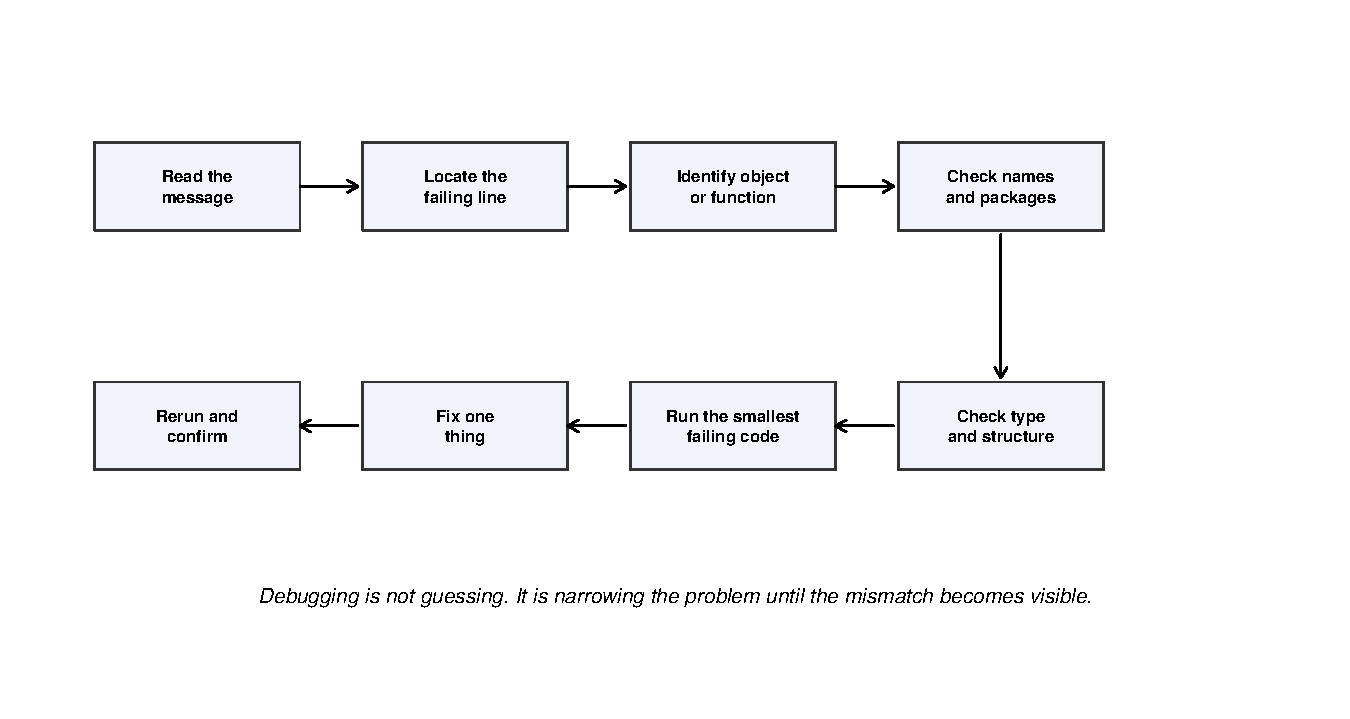
\includegraphics[width=0.9\linewidth,height=\textheight,keepaspectratio]{chapters/10-debugging-r_files/figure-pdf/fig-debugging-framework-1.pdf}

}

\caption{\label{fig-debugging-framework}A Practical Debugging Framework
for R}

\end{figure}%

As shown in Figure~\ref{fig-debugging-framework}, the process does not
begin with fixing. It begins with reading. A rushed fix can hide the
real problem. A careful diagnosis makes the fix smaller and safer.

\begin{tcolorbox}[enhanced jigsaw, arc=.35mm, bottomrule=.15mm, breakable, colback=white, colframe=quarto-callout-tip-color-frame, left=2mm, leftrule=.75mm, opacityback=0, rightrule=.15mm, toprule=.15mm]
\begin{minipage}[t]{5.5mm}
\textcolor{quarto-callout-tip-color}{\faLightbulb}
\end{minipage}%
\begin{minipage}[t]{\textwidth - 5.5mm}

\vspace{-3mm}\textbf{Debugging Habit}\vspace{3mm}

When code fails, do not immediately rewrite the whole script. First,
copy the smallest part that fails and run only that part. A smaller
problem is easier to see.

\end{minipage}%
\end{tcolorbox}

\section{Step 1: Read the Message
Slowly}\label{step-1-read-the-message-slowly}

Many beginners read only the first word:

\begin{Shaded}
\begin{Highlighting}[]
\NormalTok{Error}
\end{Highlighting}
\end{Shaded}

Then they stop thinking.

Leo needs to read beyond the emotional word. The message often contains
the most useful clue.

For example:

\begin{Shaded}
\begin{Highlighting}[]
\NormalTok{Error: object \textquotesingle{}project\_scores\textquotesingle{} not found}
\end{Highlighting}
\end{Shaded}

This message is not vague. It says R looked for an object called
\texttt{project\_scores} and could not find it.

Possible reasons include:

\begin{itemize}
\tightlist
\item
  Leo has not created the object yet;
\item
  he created it under a different name;
\item
  he misspelled it;
\item
  he used different capitalisation;
\item
  he restarted R and lost the object from the session;
\item
  the object was created inside a function and is not available outside
  it.
\end{itemize}

That is already useful.

The message has narrowed the search.

\section{Step 2: Locate the Failing
Line}\label{step-2-locate-the-failing-line}

In a short script, the failing line may be obvious. In a longer script,
Leo may not know exactly where the problem happened.

A good habit is to run code in sections. If a long script fails, Leo
should avoid changing lines at random. He should find the first line
that fails.

In RStudio, running small chunks or selected lines can help. In a Quarto
document, chunk boundaries also help. If a chunk fails, Leo can test the
code inside that chunk piece by piece.

The question is:

\begin{quote}
Which exact instruction made R stop?
\end{quote}

Until Leo knows that, he is debugging the whole script at once. That is
too large.

\section{Step 3: Debug Missing
Objects}\label{step-3-debug-missing-objects}

One of the most common R errors is:

\begin{Shaded}
\begin{Highlighting}[]
\NormalTok{Error: object \textquotesingle{}x\textquotesingle{} not found}
\end{Highlighting}
\end{Shaded}

This error usually means that R was given a name that does not exist in
the current place where R is looking.

Example:

\begin{Shaded}
\begin{Highlighting}[]
\NormalTok{project\_score}
\end{Highlighting}
\end{Shaded}

If no object called \texttt{project\_score} exists in the current
environment, R cannot guess what Leo meant.

A beginner may think, ``But the column exists in my data frame.'' That
may be true. But a column inside a data frame is not always available as
a standalone object.

For example:

\begin{Shaded}
\begin{Highlighting}[]
\NormalTok{df\_learners}\SpecialCharTok{$}\NormalTok{project\_score}
\end{Highlighting}
\end{Shaded}

is different from:

\begin{Shaded}
\begin{Highlighting}[]
\NormalTok{project\_score}
\end{Highlighting}
\end{Shaded}

The first tells R to look inside \texttt{df\_learners}. The second asks
R to find an object called \texttt{project\_score} in the current
environment.

Leo can inspect what objects exist:

\begin{Shaded}
\begin{Highlighting}[]
\FunctionTok{ls}\NormalTok{()}
\end{Highlighting}
\end{Shaded}

He can inspect the names inside a data frame:

\begin{Shaded}
\begin{Highlighting}[]
\FunctionTok{names}\NormalTok{(df\_learners)}
\end{Highlighting}
\end{Shaded}

If he is working with a data frame, this question matters:

\begin{quote}
Is this name an object by itself, or is it a column inside another
object?
\end{quote}

That question solves many early errors.

\section{Step 4: Check Spelling and
Case}\label{step-4-check-spelling-and-case}

R is case-sensitive.

These are not the same object:

\begin{Shaded}
\begin{Highlighting}[]
\NormalTok{project\_scores}
\NormalTok{Project\_scores}
\NormalTok{project\_Scores}
\end{Highlighting}
\end{Shaded}

A human reader may see them as almost identical. R does not.

This is why spelling and case should be checked before deeper
explanations are invented. Sometimes the problem is not a complex
programming issue. Sometimes the problem is one capital letter.

Consider this:

\begin{Shaded}
\begin{Highlighting}[]
\NormalTok{study\_hours }\OtherTok{\textless{}{-}} \FunctionTok{c}\NormalTok{(}\DecValTok{4}\NormalTok{, }\DecValTok{6}\NormalTok{, }\DecValTok{3}\NormalTok{, }\DecValTok{8}\NormalTok{)}

\FunctionTok{mean}\NormalTok{(study\_Hours)}
\end{Highlighting}
\end{Shaded}

R will not treat \texttt{study\_hours} and \texttt{study\_Hours} as the
same name.

A simple naming habit helps: use lower case, meaningful names, and
underscores.

\begin{Shaded}
\begin{Highlighting}[]
\NormalTok{study\_hours}
\NormalTok{project\_scores}
\NormalTok{clean\_country}
\end{Highlighting}
\end{Shaded}

Names should be boring enough to type correctly.

\begin{tcolorbox}[enhanced jigsaw, arc=.35mm, bottomrule=.15mm, breakable, colback=white, colframe=quarto-callout-warning-color-frame, left=2mm, leftrule=.75mm, opacityback=0, rightrule=.15mm, toprule=.15mm]
\begin{minipage}[t]{5.5mm}
\textcolor{quarto-callout-warning-color}{\faExclamationTriangle}
\end{minipage}%
\begin{minipage}[t]{\textwidth - 5.5mm}

\vspace{-3mm}\textbf{Common Beginner Trap}\vspace{3mm}

Do not assume that a name is correct because it looks familiar. R cares
about exact spelling. \texttt{score\_gap}, \texttt{score\_Gap}, and
\texttt{scoregap} are three different names.

\end{minipage}%
\end{tcolorbox}

\section{Step 5: Debug Assignment
Problems}\label{step-5-debug-assignment-problems}

Sometimes the object is missing because Leo did not assign it correctly.

Assignment creates a name:

\begin{Shaded}
\begin{Highlighting}[]
\NormalTok{project\_scores }\OtherTok{\textless{}{-}} \FunctionTok{c}\NormalTok{(}\DecValTok{72}\NormalTok{, }\DecValTok{81}\NormalTok{, }\DecValTok{65}\NormalTok{, }\DecValTok{90}\NormalTok{)}
\end{Highlighting}
\end{Shaded}

If Leo only writes:

\begin{Shaded}
\begin{Highlighting}[]
\FunctionTok{c}\NormalTok{(}\DecValTok{72}\NormalTok{, }\DecValTok{81}\NormalTok{, }\DecValTok{65}\NormalTok{, }\DecValTok{90}\NormalTok{)}
\end{Highlighting}
\end{Shaded}

R prints the values, but it does not store them under the name
\texttt{project\_scores}.

Later, this fails:

\begin{Shaded}
\begin{Highlighting}[]
\FunctionTok{mean}\NormalTok{(project\_scores)}
\end{Highlighting}
\end{Shaded}

because \texttt{project\_scores} was never created.

The debugging question is:

\begin{quote}
Did I create the object before using it?
\end{quote}

Order matters. R reads code from top to bottom during normal execution.
If an object is used before it is created, R cannot know about it.

This is also why restarting R and rerunning the script from the top is
useful. It tests whether the script creates everything it depends on.

A script that only works because Leo created hidden objects earlier in
the session is fragile. A reliable script can rebuild its own objects in
order.

\section{Step 6: Debug Syntax Errors}\label{step-6-debug-syntax-errors}

A syntax error means R cannot read the code as a valid instruction.

A common signal is:

\begin{Shaded}
\begin{Highlighting}[]
\NormalTok{Error: unexpected symbol}
\end{Highlighting}
\end{Shaded}

Example:

\begin{Shaded}
\begin{Highlighting}[]
\NormalTok{mean project\_scores}
\end{Highlighting}
\end{Shaded}

Leo may have intended:

\begin{Shaded}
\begin{Highlighting}[]
\FunctionTok{mean}\NormalTok{(project\_scores)}
\end{Highlighting}
\end{Shaded}

The first version is missing parentheses. R does not see a valid
function call.

Another common issue is a missing comma:

\begin{Shaded}
\begin{Highlighting}[]
\FunctionTok{data.frame}\NormalTok{(}
  \AttributeTok{learner\_id =} \FunctionTok{c}\NormalTok{(}\DecValTok{1}\NormalTok{, }\DecValTok{2}\NormalTok{, }\DecValTok{3}\NormalTok{)}
  \AttributeTok{project\_score =} \FunctionTok{c}\NormalTok{(}\DecValTok{72}\NormalTok{, }\DecValTok{81}\NormalTok{, }\DecValTok{90}\NormalTok{)}
\NormalTok{)}
\end{Highlighting}
\end{Shaded}

R expects a comma between arguments:

\begin{Shaded}
\begin{Highlighting}[]
\FunctionTok{data.frame}\NormalTok{(}
  \AttributeTok{learner\_id =} \FunctionTok{c}\NormalTok{(}\DecValTok{1}\NormalTok{, }\DecValTok{2}\NormalTok{, }\DecValTok{3}\NormalTok{),}
  \AttributeTok{project\_score =} \FunctionTok{c}\NormalTok{(}\DecValTok{72}\NormalTok{, }\DecValTok{81}\NormalTok{, }\DecValTok{90}\NormalTok{)}
\NormalTok{)}
\end{Highlighting}
\end{Shaded}

Syntax errors are often about punctuation: parentheses, commas,
quotation marks, brackets, and operators.

Leo should not treat punctuation as decoration. In R, punctuation
carries structure.

\section{Step 7: Debug Function Calls and
Arguments}\label{step-7-debug-function-calls-and-arguments}

Functions expect inputs in particular places.

A function call has a name, parentheses, and usually arguments:

\begin{Shaded}
\begin{Highlighting}[]
\FunctionTok{round}\NormalTok{(}\FloatTok{3.14159}\NormalTok{, }\AttributeTok{digits =} \DecValTok{2}\NormalTok{)}
\end{Highlighting}
\end{Shaded}

If Leo gives a function the wrong kind of input, leaves out an input, or
misspells an argument, the function may fail.

Example:

\begin{Shaded}
\begin{Highlighting}[]
\FunctionTok{round}\NormalTok{(}\StringTok{"three"}\NormalTok{, }\AttributeTok{digits =} \DecValTok{2}\NormalTok{)}
\end{Highlighting}
\end{Shaded}

The issue is not that \texttt{round()} is broken. The issue is that text
cannot be rounded as a number.

A useful debugging question is:

\begin{quote}
What kind of input does this function expect?
\end{quote}

Leo can inspect help when needed:

\begin{Shaded}
\begin{Highlighting}[]
\NormalTok{?round}
\end{Highlighting}
\end{Shaded}

He can also test with a very simple input:

\begin{Shaded}
\begin{Highlighting}[]
\FunctionTok{round}\NormalTok{(}\FloatTok{3.14159}\NormalTok{, }\AttributeTok{digits =} \DecValTok{2}\NormalTok{)}
\end{Highlighting}
\end{Shaded}

If the simple input works and the real input fails, the problem is
probably in the real input, not in the function itself.

\section{Step 8: Debug Data Type
Problems}\label{step-8-debug-data-type-problems}

Some errors happen because a value looks right to Leo but has the wrong
type inside R.

Example:

\begin{Shaded}
\begin{Highlighting}[]
\NormalTok{score }\OtherTok{\textless{}{-}} \StringTok{"72"}

\NormalTok{score }\SpecialCharTok{+} \DecValTok{5}
\end{Highlighting}
\end{Shaded}

R may respond with:

\begin{Shaded}
\begin{Highlighting}[]
\NormalTok{Error in score + 5 : non{-}numeric argument to binary operator}
\end{Highlighting}
\end{Shaded}

To Leo, \texttt{"72"} looks like a number. To R, it is character text
because it is inside quotation marks.

The debugging question is:

\begin{quote}
What type is this object?
\end{quote}

Leo can check:

\begin{Shaded}
\begin{Highlighting}[]
\FunctionTok{typeof}\NormalTok{(score)}
\FunctionTok{class}\NormalTok{(score)}
\FunctionTok{str}\NormalTok{(score)}
\end{Highlighting}
\end{Shaded}

Then he can decide whether conversion is appropriate:

\begin{Shaded}
\begin{Highlighting}[]
\NormalTok{score\_num }\OtherTok{\textless{}{-}} \FunctionTok{as.numeric}\NormalTok{(score)}
\NormalTok{score\_num }\SpecialCharTok{+} \DecValTok{5}
\end{Highlighting}
\end{Shaded}

But conversion should not be automatic or careless. If text values
include \texttt{"not\ available"} or \texttt{"missing"}, conversion can
introduce \texttt{NA} values. That may be correct, but Leo should notice
it.

Types are not cosmetic. Types determine what R can safely do.

\section{Step 9: Debug Structure
Problems}\label{step-9-debug-structure-problems}

Sometimes the type is not the only issue. The structure is wrong.

A vector, list, matrix, and data frame do not behave the same way. A
column may be inside a data frame. A value may be inside a list. A row
may not exist. An index may be too large.

A common error is:

\begin{Shaded}
\begin{Highlighting}[]
\NormalTok{subscript out of bounds}
\end{Highlighting}
\end{Shaded}

This often means Leo asked for an element that does not exist.

Example:

\begin{Shaded}
\begin{Highlighting}[]
\NormalTok{scores }\OtherTok{\textless{}{-}} \FunctionTok{c}\NormalTok{(}\DecValTok{72}\NormalTok{, }\DecValTok{81}\NormalTok{, }\DecValTok{90}\NormalTok{)}

\NormalTok{scores[}\DecValTok{4}\NormalTok{]}
\end{Highlighting}
\end{Shaded}

For vectors, this particular request returns \texttt{NA}, but similar
out-of-range requests in matrices, arrays, or lists can produce errors.
The principle is the same: Leo asked for a position outside the
available structure.

A common list example:

\begin{Shaded}
\begin{Highlighting}[]
\NormalTok{learner }\OtherTok{\textless{}{-}} \FunctionTok{list}\NormalTok{(}
  \AttributeTok{name =} \StringTok{"Leo"}\NormalTok{,}
  \AttributeTok{score =} \DecValTok{82}
\NormalTok{)}

\NormalTok{learner[[}\DecValTok{3}\NormalTok{]]}
\end{Highlighting}
\end{Shaded}

There is no third element.

Before extracting, Leo should inspect:

\begin{Shaded}
\begin{Highlighting}[]
\FunctionTok{str}\NormalTok{(learner)}
\FunctionTok{length}\NormalTok{(learner)}
\FunctionTok{names}\NormalTok{(learner)}
\end{Highlighting}
\end{Shaded}

The debugging question is:

\begin{quote}
What is the structure of this object, and does the part I am asking for
exist?
\end{quote}

\section{Step 10: Debug Data Frame Column
Names}\label{step-10-debug-data-frame-column-names}

Another common problem appears when Leo tries to use a column name that
does not exist.

Example:

\begin{Shaded}
\begin{Highlighting}[]
\NormalTok{df\_learners }\OtherTok{\textless{}{-}} \FunctionTok{data.frame}\NormalTok{(}
  \AttributeTok{learner\_id =} \FunctionTok{c}\NormalTok{(}\DecValTok{1}\NormalTok{, }\DecValTok{2}\NormalTok{, }\DecValTok{3}\NormalTok{),}
  \AttributeTok{project\_score =} \FunctionTok{c}\NormalTok{(}\DecValTok{72}\NormalTok{, }\DecValTok{81}\NormalTok{, }\DecValTok{90}\NormalTok{)}
\NormalTok{)}

\NormalTok{df\_learners}\SpecialCharTok{$}\NormalTok{project\_scores}
\end{Highlighting}
\end{Shaded}

The actual column is \texttt{project\_score}, not
\texttt{project\_scores}.

With \texttt{\$}, R may return \texttt{NULL} rather than a loud error.
That can be dangerous because the code does not always fail immediately.

Leo should inspect the names:

\begin{Shaded}
\begin{Highlighting}[]
\FunctionTok{names}\NormalTok{(df\_learners)}
\end{Highlighting}
\end{Shaded}

In later chapters, this habit becomes essential. Imported data may have
spaces, capital letters, unexpected punctuation, or names that differ
from what Leo remembers.

For now, the rule is simple:

\begin{quote}
Before using a column name, inspect the column names.
\end{quote}

\section{Step 11: Debug Package and Namespace
Problems}\label{step-11-debug-package-and-namespace-problems}

Sometimes R cannot find a function because the function does not belong
to base R or because the package that contains it has not been loaded.

A common message is:

\begin{Shaded}
\begin{Highlighting}[]
\NormalTok{Error: could not find function "filter"}
\end{Highlighting}
\end{Shaded}

This may happen if Leo tries to use a function from a package that is
not available in the current session.

For example:

\begin{Shaded}
\begin{Highlighting}[]
\FunctionTok{filter}\NormalTok{(df\_learners, project\_score }\SpecialCharTok{\textgreater{}=} \DecValTok{80}\NormalTok{)}
\end{Highlighting}
\end{Shaded}

If the relevant package is not loaded, R may not know which
\texttt{filter()} Leo means.

One solution is to load the package:

\begin{Shaded}
\begin{Highlighting}[]
\FunctionTok{library}\NormalTok{(dplyr)}
\end{Highlighting}
\end{Shaded}

Another is to use the namespace directly:

\begin{Shaded}
\begin{Highlighting}[]
\NormalTok{dplyr}\SpecialCharTok{::}\FunctionTok{filter}\NormalTok{(df\_learners, project\_score }\SpecialCharTok{\textgreater{}=} \DecValTok{80}\NormalTok{)}
\end{Highlighting}
\end{Shaded}

This chapter will not teach packages in full. That is the job of Chapter
11. Here, Leo only needs one debugging insight:

\begin{quote}
If R cannot find a function, check spelling first, then check whether
the function comes from a package.
\end{quote}

This prepares him for the next chapter, where packages become a central
workflow tool.

\section{Step 12: Debug Pipes}\label{step-12-debug-pipes}

The pipe is useful because it lets Leo read a sequence of actions from
left to right.

But a pipe can also hide where a problem begins if Leo runs a long chain
all at once.

Example:

\begin{Shaded}
\begin{Highlighting}[]
\NormalTok{df\_learners }\SpecialCharTok{|\textgreater{}}
\NormalTok{  dplyr}\SpecialCharTok{::}\FunctionTok{filter}\NormalTok{(project\_score }\SpecialCharTok{\textgreater{}=} \DecValTok{80}\NormalTok{) }\SpecialCharTok{|\textgreater{}}
\NormalTok{  dplyr}\SpecialCharTok{::}\FunctionTok{mutate}\NormalTok{(}\AttributeTok{score\_gap =}\NormalTok{ project\_score }\SpecialCharTok{{-}}\NormalTok{ pre\_assessment\_score) }\SpecialCharTok{|\textgreater{}}
\NormalTok{  dplyr}\SpecialCharTok{::}\FunctionTok{summarise}\NormalTok{(}\AttributeTok{mean\_gap =} \FunctionTok{mean}\NormalTok{(score\_gap, }\AttributeTok{na.rm =} \ConstantTok{TRUE}\NormalTok{))}
\end{Highlighting}
\end{Shaded}

If this fails, Leo should not stare at the whole pipe as one mystery. He
should build it one step at a time.

First:

\begin{Shaded}
\begin{Highlighting}[]
\NormalTok{df\_learners }\SpecialCharTok{|\textgreater{}}
\NormalTok{  dplyr}\SpecialCharTok{::}\FunctionTok{filter}\NormalTok{(project\_score }\SpecialCharTok{\textgreater{}=} \DecValTok{80}\NormalTok{)}
\end{Highlighting}
\end{Shaded}

Then:

\begin{Shaded}
\begin{Highlighting}[]
\NormalTok{df\_learners }\SpecialCharTok{|\textgreater{}}
\NormalTok{  dplyr}\SpecialCharTok{::}\FunctionTok{filter}\NormalTok{(project\_score }\SpecialCharTok{\textgreater{}=} \DecValTok{80}\NormalTok{) }\SpecialCharTok{|\textgreater{}}
\NormalTok{  dplyr}\SpecialCharTok{::}\FunctionTok{mutate}\NormalTok{(}\AttributeTok{score\_gap =}\NormalTok{ project\_score }\SpecialCharTok{{-}}\NormalTok{ pre\_assessment\_score)}
\end{Highlighting}
\end{Shaded}

Then:

\begin{Shaded}
\begin{Highlighting}[]
\NormalTok{df\_learners }\SpecialCharTok{|\textgreater{}}
\NormalTok{  dplyr}\SpecialCharTok{::}\FunctionTok{filter}\NormalTok{(project\_score }\SpecialCharTok{\textgreater{}=} \DecValTok{80}\NormalTok{) }\SpecialCharTok{|\textgreater{}}
\NormalTok{  dplyr}\SpecialCharTok{::}\FunctionTok{mutate}\NormalTok{(}\AttributeTok{score\_gap =}\NormalTok{ project\_score }\SpecialCharTok{{-}}\NormalTok{ pre\_assessment\_score) }\SpecialCharTok{|\textgreater{}}
\NormalTok{  dplyr}\SpecialCharTok{::}\FunctionTok{summarise}\NormalTok{(}\AttributeTok{mean\_gap =} \FunctionTok{mean}\NormalTok{(score\_gap, }\AttributeTok{na.rm =} \ConstantTok{TRUE}\NormalTok{))}
\end{Highlighting}
\end{Shaded}

This approach narrows the failure.

A pipe is a chain. To debug a chain, test the links.

\begin{tcolorbox}[enhanced jigsaw, arc=.35mm, bottomrule=.15mm, breakable, colback=white, colframe=quarto-callout-tip-color-frame, left=2mm, leftrule=.75mm, opacityback=0, rightrule=.15mm, toprule=.15mm]
\begin{minipage}[t]{5.5mm}
\textcolor{quarto-callout-tip-color}{\faLightbulb}
\end{minipage}%
\begin{minipage}[t]{\textwidth - 5.5mm}

\vspace{-3mm}\textbf{Debugging Habit}\vspace{3mm}

When a pipe fails, run the first line, then the first two lines, then
the first three. The first step that fails is the place to inspect.

\end{minipage}%
\end{tcolorbox}

\section{Step 13: Debug User-Defined
Functions}\label{step-13-debug-user-defined-functions}

Chapter 9 taught Leo to write functions. Chapter 10 now teaches him how
to test them.

Suppose Leo writes:

\begin{Shaded}
\begin{Highlighting}[]
\NormalTok{score\_gap }\OtherTok{\textless{}{-}} \ControlFlowTok{function}\NormalTok{(project\_score, pre\_score) \{}
\NormalTok{  project\_score }\SpecialCharTok{{-}}\NormalTok{ pre\_assessment\_score}
\NormalTok{\}}
\end{Highlighting}
\end{Shaded}

Then he runs:

\begin{Shaded}
\begin{Highlighting}[]
\FunctionTok{score\_gap}\NormalTok{(}\DecValTok{85}\NormalTok{, }\DecValTok{70}\NormalTok{)}
\end{Highlighting}
\end{Shaded}

R may complain that \texttt{pre\_assessment\_score} is not found.

Why? The function argument is called \texttt{pre\_score}, but inside the
function Leo used \texttt{pre\_assessment\_score}.

A corrected version is:

\begin{Shaded}
\begin{Highlighting}[]
\NormalTok{score\_gap }\OtherTok{\textless{}{-}} \ControlFlowTok{function}\NormalTok{(project\_score, pre\_score) \{}
\NormalTok{  project\_score }\SpecialCharTok{{-}}\NormalTok{ pre\_score}
\NormalTok{\}}

\FunctionTok{score\_gap}\NormalTok{(}\DecValTok{85}\NormalTok{, }\DecValTok{70}\NormalTok{)}
\end{Highlighting}
\end{Shaded}

When debugging a function, Leo should ask:

\begin{Shaded}
\begin{Highlighting}[]
\NormalTok{Are the argument names consistent?}
\NormalTok{Does the function use objects that exist inside the function?}
\NormalTok{Have I tested it with one simple input?}
\NormalTok{Does the output match what I expected?}
\end{Highlighting}
\end{Shaded}

The best first test for a function is not the full dataset. It is a
simple case Leo can check in his head.

\begin{Shaded}
\begin{Highlighting}[]
\FunctionTok{score\_gap}\NormalTok{(}\DecValTok{85}\NormalTok{, }\DecValTok{70}\NormalTok{)}
\end{Highlighting}
\end{Shaded}

The expected answer is \texttt{15}. If that fails, the function needs
attention before it is used in a larger workflow.

\section{Step 14: Run the Smallest Failing
Code}\label{step-14-run-the-smallest-failing-code}

This is one of the most important debugging habits in the book.

When a script fails, Leo should not bring the whole script to the
problem. He should reduce the problem until the failure is small enough
to understand.

Suppose this fails:

\begin{Shaded}
\begin{Highlighting}[]
\NormalTok{df\_learners }\SpecialCharTok{|\textgreater{}}
\NormalTok{  dplyr}\SpecialCharTok{::}\FunctionTok{filter}\NormalTok{(country }\SpecialCharTok{==} \StringTok{"Nigeria"}\NormalTok{) }\SpecialCharTok{|\textgreater{}}
\NormalTok{  dplyr}\SpecialCharTok{::}\FunctionTok{mutate}\NormalTok{(}\AttributeTok{score\_gap =}\NormalTok{ project\_score }\SpecialCharTok{{-}}\NormalTok{ pre\_assessment\_score) }\SpecialCharTok{|\textgreater{}}
\NormalTok{  dplyr}\SpecialCharTok{::}\FunctionTok{group\_by}\NormalTok{(background) }\SpecialCharTok{|\textgreater{}}
\NormalTok{  dplyr}\SpecialCharTok{::}\FunctionTok{summarise}\NormalTok{(}\AttributeTok{mean\_gap =} \FunctionTok{mean}\NormalTok{(score\_gap, }\AttributeTok{na.rm =} \ConstantTok{TRUE}\NormalTok{))}
\end{Highlighting}
\end{Shaded}

Leo can ask:

\begin{Shaded}
\begin{Highlighting}[]
\NormalTok{Does df\_learners exist?}
\NormalTok{Does country exist?}
\NormalTok{Does project\_score exist?}
\NormalTok{Does pre\_assessment\_score exist?}
\NormalTok{Does the filter step work alone?}
\NormalTok{Does the mutate step work after filtering?}
\end{Highlighting}
\end{Shaded}

He can inspect:

\begin{Shaded}
\begin{Highlighting}[]
\FunctionTok{names}\NormalTok{(df\_learners)}
\FunctionTok{str}\NormalTok{(df\_learners)}
\end{Highlighting}
\end{Shaded}

Then run one part:

\begin{Shaded}
\begin{Highlighting}[]
\NormalTok{df\_learners }\SpecialCharTok{|\textgreater{}}
\NormalTok{  dplyr}\SpecialCharTok{::}\FunctionTok{filter}\NormalTok{(country }\SpecialCharTok{==} \StringTok{"Nigeria"}\NormalTok{)}
\end{Highlighting}
\end{Shaded}

A small failing example is not a beginner trick. It is professional
discipline.

It also helps when asking for help. A person who can show a small
failing example is much easier to help than a person who only says, ``My
code does not work.''

In R communities, this is often called creating a reproducible example,
or reprex. Leo does not need to master the full practice now. He only
needs the habit of making the problem smaller and clearer.

\section{Step 15: Fix One Thing at a
Time}\label{step-15-fix-one-thing-at-a-time}

A common beginner response to errors is to change many things at once.

Leo changes an object name, moves a line, adds a package, edits a
function, and reruns the script. The error changes. Now he does not know
which change mattered.

A calmer method is:

\begin{Shaded}
\begin{Highlighting}[]
\NormalTok{Change one thing.}
\NormalTok{Run again.}
\NormalTok{Observe what changed.}
\NormalTok{Then decide the next step.}
\end{Highlighting}
\end{Shaded}

This is slower for one minute and faster for the whole project.

Debugging is not only about finding the fix. It is about preserving
evidence while finding the fix.

\section{Common R Errors and First
Questions}\label{common-r-errors-and-first-questions}

The table below is not a replacement for the framework. It is a quick
reference for common signals Leo is likely to meet.

\begin{longtable}[]{@{}
  >{\raggedright\arraybackslash}p{(\linewidth - 4\tabcolsep) * \real{0.3333}}
  >{\raggedright\arraybackslash}p{(\linewidth - 4\tabcolsep) * \real{0.3333}}
  >{\raggedright\arraybackslash}p{(\linewidth - 4\tabcolsep) * \real{0.3333}}@{}}
\caption{Common R Errors and First Diagnostic
Questions}\label{tbl-common-errors}\tabularnewline
\toprule\noalign{}
\begin{minipage}[b]{\linewidth}\raggedright
Error or signal
\end{minipage} & \begin{minipage}[b]{\linewidth}\raggedright
Usual meaning
\end{minipage} & \begin{minipage}[b]{\linewidth}\raggedright
First question Leo should ask
\end{minipage} \\
\midrule\noalign{}
\endfirsthead
\toprule\noalign{}
\begin{minipage}[b]{\linewidth}\raggedright
Error or signal
\end{minipage} & \begin{minipage}[b]{\linewidth}\raggedright
Usual meaning
\end{minipage} & \begin{minipage}[b]{\linewidth}\raggedright
First question Leo should ask
\end{minipage} \\
\midrule\noalign{}
\endhead
\bottomrule\noalign{}
\endlastfoot
\texttt{object\ \textquotesingle{}x\textquotesingle{}\ not\ found} & R
cannot find an object with that name. & Did I create the object before
using it, and is the spelling exact? \\
\texttt{could\ not\ find\ function} & The function name is unknown in
the current session. & Did I spell the function correctly, and does it
come from a package? \\
\texttt{unexpected\ symbol} & R cannot parse the instruction. & Am I
missing a comma, parenthesis, operator, or quotation mark? \\
\texttt{non-numeric\ argument\ to\ binary\ operator} & A calculation
used something that is not numeric. & Is one of the values stored as
text or another type? \\
\texttt{subscript\ out\ of\ bounds} & Code requested a position or
element that does not exist. & What is the length, dimension, or
structure of the object? \\
\texttt{object\ of\ type\ \textquotesingle{}closure\textquotesingle{}\ is\ not\ subsettable}
& Code is trying to subset a function as if it were data. & Did I use
the same name for a function and an object, or forget parentheses? \\
\texttt{NAs\ introduced\ by\ coercion} & R converted values and created
missing values where conversion failed. & Which values could not be
converted, and is that expected? \\
Replacement length mismatch & Code tried to replace values with a vector
of the wrong length. & How many values am I replacing, and how many
replacement values did I provide? \\
\end{longtable}

Table~\ref{tbl-common-errors} is deliberately practical. It does not ask
Leo to memorise every possible cause. It gives him a first question.
Debugging begins with better questions.

\section{\texorpdfstring{A Closer Look:
\texttt{object\ of\ type\ \textquotesingle{}closure\textquotesingle{}\ is\ not\ subsettable}}{A Closer Look: object of type \textquotesingle closure\textquotesingle{} is not subsettable}}\label{a-closer-look-object-of-type-closure-is-not-subsettable}

This error looks strange, so it deserves a short explanation.

In R, a function is sometimes described internally as a closure. If Leo
tries to subset a function as though it were a vector or data frame, R
may complain.

Example:

\begin{Shaded}
\begin{Highlighting}[]
\NormalTok{mean[}\DecValTok{1}\NormalTok{]}
\end{Highlighting}
\end{Shaded}

\texttt{mean} is a function. Leo probably meant to call it with
parentheses:

\begin{Shaded}
\begin{Highlighting}[]
\FunctionTok{mean}\NormalTok{(}\FunctionTok{c}\NormalTok{(}\DecValTok{72}\NormalTok{, }\DecValTok{81}\NormalTok{, }\DecValTok{90}\NormalTok{))}
\end{Highlighting}
\end{Shaded}

Another common cause is naming an object in a way that conflicts with a
function name.

\begin{Shaded}
\begin{Highlighting}[]
\NormalTok{data }\OtherTok{\textless{}{-}} \FunctionTok{data.frame}\NormalTok{(}\AttributeTok{score =} \FunctionTok{c}\NormalTok{(}\DecValTok{72}\NormalTok{, }\DecValTok{81}\NormalTok{, }\DecValTok{90}\NormalTok{))}
\end{Highlighting}
\end{Shaded}

Using \texttt{data} as an object name can be confusing because
\texttt{data()} is also a function. This does not always break code, but
it can make errors harder to interpret.

The practical habit is simple: choose clear object names and remember
the difference between calling a function with \texttt{()} and
extracting from an object with \texttt{{[}{]}}, \texttt{{[}{[}\ {]}{]}},
or \texttt{\$}.

\section{\texorpdfstring{When to Use
\texttt{traceback()}}{When to Use traceback()}}\label{when-to-use-traceback}

Sometimes an error comes from a function calling another function inside
it. The visible error may not show the whole path.

Base R provides:

\begin{Shaded}
\begin{Highlighting}[]
\FunctionTok{traceback}\NormalTok{()}
\end{Highlighting}
\end{Shaded}

This can show the sequence of calls that led to the last error.

For many beginners, \texttt{traceback()} output may look dense. Leo does
not need to master it now. He only needs to know that it exists and that
it can sometimes help locate where an error came from.

Some tidyverse workflows also provide richer error traces through tools
such as \texttt{rlang::last\_trace()}. That can be useful later,
especially when working with packages. But the beginner method remains
the same: read the message, locate the failing step, inspect the object,
and reduce the problem.

\section{Debugging Checklist}\label{debugging-checklist}

Before searching online or asking someone else, Leo can walk through
this checklist:

\begin{Shaded}
\begin{Highlighting}[]
\NormalTok{1. Did I read the full error, warning, or message?}
\NormalTok{2. Which exact line failed?}
\NormalTok{3. Which object or function is mentioned?}
\NormalTok{4. Does the object exist?}
\NormalTok{5. Is the spelling and capitalisation exact?}
\NormalTok{6. Did I create the object before using it?}
\NormalTok{7. Is the function name correct?}
\NormalTok{8. Does the function come from a package?}
\NormalTok{9. Is the package loaded or is the namespace explicit?}
\NormalTok{10. What type is the object?}
\NormalTok{11. What structure does the object have?}
\NormalTok{12. Can I run a smaller version of the failing code?}
\NormalTok{13. Did I change only one thing before rerunning?}
\NormalTok{14. Did the fix actually solve the original problem?}
\end{Highlighting}
\end{Shaded}

This checklist is not meant to slow Leo down forever. With practice,
these questions become automatic.

\section{Cheat Sheet: Common Errors and First
Moves}\label{cheat-sheet-common-errors-and-first-moves}

This short cheat sheet is for quick memory.

\begin{Shaded}
\begin{Highlighting}[]
\NormalTok{object not found}
\NormalTok{→ Check spelling, case, assignment, and whether the object exists.}

\NormalTok{could not find function}
\NormalTok{→ Check spelling, package loading, and package::function().}

\NormalTok{unexpected symbol}
\NormalTok{→ Check commas, parentheses, quotation marks, and operators.}

\NormalTok{non{-}numeric argument}
\NormalTok{→ Check type with str(), typeof(), or class().}

\NormalTok{subscript out of bounds}
\NormalTok{→ Check length(), dim(), names(), and str().}

\NormalTok{NAs introduced by coercion}
\NormalTok{→ Check which values failed conversion.}

\NormalTok{pipe fails}
\NormalTok{→ Run the pipe one step at a time.}

\NormalTok{function fails}
\NormalTok{→ Test the function with one simple input.}

\NormalTok{warning appears}
\NormalTok{→ Inspect the result before trusting it.}

\NormalTok{message appears}
\NormalTok{→ Read it, then decide whether action is needed.}
\end{Highlighting}
\end{Shaded}

The goal is not to know every answer immediately. The goal is to know
the first sensible move.

\section{Try It Yourself}\label{try-it-yourself-1}

Create a simple object:

\begin{Shaded}
\begin{Highlighting}[]
\NormalTok{project\_scores }\OtherTok{\textless{}{-}} \FunctionTok{c}\NormalTok{(}\DecValTok{72}\NormalTok{, }\DecValTok{81}\NormalTok{, }\DecValTok{65}\NormalTok{, }\DecValTok{90}\NormalTok{)}
\end{Highlighting}
\end{Shaded}

Now intentionally run this:

\begin{Shaded}
\begin{Highlighting}[]
\FunctionTok{mean}\NormalTok{(project\_score)}
\end{Highlighting}
\end{Shaded}

Ask:

\begin{Shaded}
\begin{Highlighting}[]
\NormalTok{What object did R look for?}
\NormalTok{What object actually exists?}
\NormalTok{What is the spelling difference?}
\end{Highlighting}
\end{Shaded}

Now correct it:

\begin{Shaded}
\begin{Highlighting}[]
\FunctionTok{mean}\NormalTok{(project\_scores)}
\end{Highlighting}
\end{Shaded}

Next, try this:

\begin{Shaded}
\begin{Highlighting}[]
\NormalTok{score }\OtherTok{\textless{}{-}} \StringTok{"72"}
\NormalTok{score }\SpecialCharTok{+} \DecValTok{5}
\end{Highlighting}
\end{Shaded}

Ask:

\begin{Shaded}
\begin{Highlighting}[]
\NormalTok{Why does this fail?}
\NormalTok{What type is score?}
\end{Highlighting}
\end{Shaded}

Check:

\begin{Shaded}
\begin{Highlighting}[]
\FunctionTok{str}\NormalTok{(score)}
\end{Highlighting}
\end{Shaded}

Then convert carefully:

\begin{Shaded}
\begin{Highlighting}[]
\NormalTok{score\_num }\OtherTok{\textless{}{-}} \FunctionTok{as.numeric}\NormalTok{(score)}
\NormalTok{score\_num }\SpecialCharTok{+} \DecValTok{5}
\end{Highlighting}
\end{Shaded}

The aim is not to create errors for entertainment. The aim is to
recognise patterns before they appear in a larger workflow.

\section{A Small Practice Lab}\label{a-small-practice-lab-2}

Use this small data frame:

\begin{Shaded}
\begin{Highlighting}[]
\NormalTok{df\_learners }\OtherTok{\textless{}{-}} \FunctionTok{data.frame}\NormalTok{(}
  \AttributeTok{learner\_id =} \FunctionTok{c}\NormalTok{(}\DecValTok{1}\NormalTok{, }\DecValTok{2}\NormalTok{, }\DecValTok{3}\NormalTok{, }\DecValTok{4}\NormalTok{),}
  \AttributeTok{country =} \FunctionTok{c}\NormalTok{(}\StringTok{"Nigeria"}\NormalTok{, }\StringTok{"Ghana"}\NormalTok{, }\StringTok{"Kenya"}\NormalTok{, }\StringTok{"Nigeria"}\NormalTok{),}
  \AttributeTok{project\_score =} \FunctionTok{c}\NormalTok{(}\DecValTok{72}\NormalTok{, }\DecValTok{81}\NormalTok{, }\DecValTok{65}\NormalTok{, }\DecValTok{90}\NormalTok{),}
  \AttributeTok{pre\_assessment\_score =} \FunctionTok{c}\NormalTok{(}\DecValTok{60}\NormalTok{, }\DecValTok{70}\NormalTok{, }\DecValTok{58}\NormalTok{, }\DecValTok{75}\NormalTok{)}
\NormalTok{)}
\end{Highlighting}
\end{Shaded}

Now run this code and debug it step by step:

\begin{Shaded}
\begin{Highlighting}[]
\NormalTok{df\_learners }\SpecialCharTok{|\textgreater{}}
\NormalTok{  dplyr}\SpecialCharTok{::}\FunctionTok{filter}\NormalTok{(country }\SpecialCharTok{==} \StringTok{"Nigeria"}\NormalTok{) }\SpecialCharTok{|\textgreater{}}
\NormalTok{  dplyr}\SpecialCharTok{::}\FunctionTok{mutate}\NormalTok{(}\AttributeTok{score\_gap =}\NormalTok{ project\_scores }\SpecialCharTok{{-}}\NormalTok{ pre\_assessment\_score) }\SpecialCharTok{|\textgreater{}}
\NormalTok{  dplyr}\SpecialCharTok{::}\FunctionTok{summarise}\NormalTok{(}\AttributeTok{mean\_gap =} \FunctionTok{mean}\NormalTok{(score\_gap, }\AttributeTok{na.rm =} \ConstantTok{TRUE}\NormalTok{))}
\end{Highlighting}
\end{Shaded}

The problem is in this part:

\begin{Shaded}
\begin{Highlighting}[]
\NormalTok{project\_scores}
\end{Highlighting}
\end{Shaded}

The column is called:

\begin{Shaded}
\begin{Highlighting}[]
\NormalTok{project\_score}
\end{Highlighting}
\end{Shaded}

A corrected version is:

\begin{Shaded}
\begin{Highlighting}[]
\NormalTok{df\_learners }\SpecialCharTok{|\textgreater{}}
\NormalTok{  dplyr}\SpecialCharTok{::}\FunctionTok{filter}\NormalTok{(country }\SpecialCharTok{==} \StringTok{"Nigeria"}\NormalTok{) }\SpecialCharTok{|\textgreater{}}
\NormalTok{  dplyr}\SpecialCharTok{::}\FunctionTok{mutate}\NormalTok{(}\AttributeTok{score\_gap =}\NormalTok{ project\_score }\SpecialCharTok{{-}}\NormalTok{ pre\_assessment\_score) }\SpecialCharTok{|\textgreater{}}
\NormalTok{  dplyr}\SpecialCharTok{::}\FunctionTok{summarise}\NormalTok{(}\AttributeTok{mean\_gap =} \FunctionTok{mean}\NormalTok{(score\_gap, }\AttributeTok{na.rm =} \ConstantTok{TRUE}\NormalTok{))}
\end{Highlighting}
\end{Shaded}

To debug the pipe, Leo should run:

\begin{Shaded}
\begin{Highlighting}[]
\NormalTok{df\_learners }\SpecialCharTok{|\textgreater{}}
\NormalTok{  dplyr}\SpecialCharTok{::}\FunctionTok{filter}\NormalTok{(country }\SpecialCharTok{==} \StringTok{"Nigeria"}\NormalTok{)}
\end{Highlighting}
\end{Shaded}

Then:

\begin{Shaded}
\begin{Highlighting}[]
\NormalTok{df\_learners }\SpecialCharTok{|\textgreater{}}
\NormalTok{  dplyr}\SpecialCharTok{::}\FunctionTok{filter}\NormalTok{(country }\SpecialCharTok{==} \StringTok{"Nigeria"}\NormalTok{) }\SpecialCharTok{|\textgreater{}}
\NormalTok{  dplyr}\SpecialCharTok{::}\FunctionTok{mutate}\NormalTok{(}\AttributeTok{score\_gap =}\NormalTok{ project\_score }\SpecialCharTok{{-}}\NormalTok{ pre\_assessment\_score)}
\end{Highlighting}
\end{Shaded}

Then the full version.

That is the framework in action.

\section{Short Recap}\label{short-recap-1}

Leo has learned that debugging is not a side issue. It is part of
becoming independent in R.

The main ideas are:

\begin{itemize}
\tightlist
\item
  errors, warnings, and messages are different kinds of signals;
\item
  an error usually means R cannot continue;
\item
  a warning means R continued but Leo should inspect the result;
\item
  a message gives information and should be read calmly;
\item
  debugging starts with reading, not guessing;
\item
  missing objects often come from spelling, order, assignment, or scope;
\item
  function errors often come from wrong inputs, missing arguments, or
  unavailable packages;
\item
  type and structure determine what R can safely do;
\item
  pipes should be debugged one step at a time;
\item
  user-defined functions should be tested with simple inputs;
\item
  the smallest failing code is easier to understand than a large failing
  script;
\item
  changing one thing at a time protects the debugging process.
\end{itemize}

The lightbulb remains:

\begin{quote}
An error message is not R refusing to help. It is R telling Leo where
the conversation broke down.
\end{quote}

\section{Leo's Notebook}\label{leos-notebook-4}

Leo writes:

\begin{quote}
When R gives me an error, I should not panic. I should read it as a
signal.
\end{quote}

He adds:

\begin{quote}
My first question is not ``Why is R broken?'' My first question is
``What did R receive, and what did it expect?''
\end{quote}

Then he writes:

\begin{quote}
I should debug small. Run the smallest failing code. Fix one thing.
Rerun. Confirm.
\end{quote}

One final note feels especially important:

\begin{quote}
If I can debug, I am no longer dependent on perfect copied code. I can
repair my own work.
\end{quote}

That is the real shift.

\section{Glossary}\label{glossary-1}

\textbf{Error}\\
A signal that R cannot continue with the instruction as written.

\textbf{Warning}\\
A signal that R completed an action, but the result may need inspection.

\textbf{Message}\\
Information printed by R or a package about what happened.

\textbf{Debugging}\\
The process of finding and fixing the mismatch between what the user
intended and what R received.

\textbf{Object}\\
A named value, vector, data frame, function, or other structure stored
in R.

\textbf{Function}\\
A named action that takes inputs, performs work, and usually returns
output.

\textbf{Argument}\\
An input given to a function.

\textbf{Package}\\
A collection of functions and resources that extends what R can do.

\textbf{Namespace}\\
The place where a package keeps its functions and objects.

\textbf{Data type}\\
The kind of value R is working with, such as numeric, character,
logical, or date.

\textbf{Structure}\\
The arrangement of values inside an object, such as vector, list,
matrix, or data frame.

\textbf{Pipeline}\\
A sequence of operations connected by a pipe.

\textbf{Reprex}\\
A small reproducible example that shows a problem clearly enough for
another person to understand and test.

\textbf{Trace}\\
A record of function calls that led to an error.

\section{Chapter Outcome}\label{chapter-outcome-9}

By the end of this chapter, Leo can:

\begin{itemize}
\tightlist
\item
  explain why errors are part of learning R;
\item
  distinguish errors, warnings, and messages;
\item
  use a step-by-step debugging framework;
\item
  inspect objects before acting on them;
\item
  diagnose common object-name and function-name errors;
\item
  recognise package-related errors;
\item
  recognise type-related and structure-related errors;
\item
  debug a pipe one step at a time;
\item
  test a user-defined function with simple inputs;
\item
  prepare a clearer question when asking for help.
\end{itemize}

These are not minor skills.

They are the habits that help Leo move from hoping code works to
understanding why it does or does not work.

\section{Closing Part 2: Leo Can Repair the
Conversation}\label{closing-part-2-leo-can-repair-the-conversation}

Part 2 began with the language of R.

Leo learned that syntax is not decoration. It is structure. He learned
that logic helps R make decisions. He learned that functions are named
actions. He learned that he can create functions of his own when
repeated logic deserves a name.

Chapter 10 adds the final maturity step.

Leo now knows that writing R is not only about producing correct code on
the first attempt. It is also about repairing code when the instruction,
object, function, type, structure, or package context is wrong.

That matters because real analysis rarely unfolds perfectly.

A learner who cannot debug remains dependent on luck, copying, and
external rescue. A learner who can debug begins to gain control.

Part 2 has therefore done more than teach Leo how R thinks and speaks.
It has taught him how to continue the conversation when it breaks.

\section{What Comes Next}\label{what-comes-next-3}

Leo is now ready to leave isolated language lessons and enter larger
workflows.

But larger workflows need more than base R. They need tools for
importing data, shaping data, visualising patterns, working with dates
and text, and making results reproducible. Some tools are already built
into R. Others come from packages.

Chapter 11 begins there.

It shows how packages extend R's working system, how those tools enter a
session, why installing and loading are different, and why reproducible
analysis depends on knowing which tools are being used.

Debugging has prepared Leo for that move. Missing packages, unloaded
packages, function conflicts, and namespace problems are all easier to
face when he already knows how to read errors as signals.

Leo now knows how to repair the conversation.

Next, he learns how R gains new tools without losing workflow control.

\part{Part 3: Data Workflows: From Isolated Commands to Reproducible
Analysis}

\chapter{Packages and the R Ecosystem in Practice: From Tools to
Reproducible
Workflows}\label{packages-and-the-r-ecosystem-in-practice-from-tools-to-reproducible-workflows}

\renewcommand{\thefigure}{11.\arabic{figure}}
\setcounter{figure}{0}
\renewcommand{\thetable}{11.\arabic{table}}
\setcounter{table}{0}

\section{Opening Scene: When R Becomes Bigger Than Base
R}\label{opening-scene-when-r-becomes-bigger-than-base-r}

Leo has just finished Part 2 with a new kind of confidence.

R no longer looks like a wall of strange symbols. He can read code as
structured meaning. He knows that operators help R calculate, compare,
assign, extract, and decide. He knows that built-in functions are
ready-made actions. He has learned to write small functions of his own
when repeated code starts to feel like a warning sign. He has also
learned that errors are not signs of failure. They are signals that help
him find where the conversation between his code and R has broken down.

For a moment, it feels as if base R might be enough.

Then he opens a real data analysis tutorial and sees this near the top:

\begin{Shaded}
\begin{Highlighting}[]
\FunctionTok{library}\NormalTok{(dplyr)}
\FunctionTok{library}\NormalTok{(readr)}
\FunctionTok{library}\NormalTok{(ggplot2)}
\end{Highlighting}
\end{Shaded}

A few lines later, he sees something like this:

\begin{Shaded}
\begin{Highlighting}[]
\NormalTok{df\_r\_migration }\SpecialCharTok{|\textgreater{}}
  \FunctionTok{filter}\NormalTok{(project\_score }\SpecialCharTok{\textgreater{}=} \DecValTok{80}\NormalTok{) }\SpecialCharTok{|\textgreater{}}
  \FunctionTok{summarise}\NormalTok{(}\AttributeTok{mean\_hours =} \FunctionTok{mean}\NormalTok{(study\_hours, }\AttributeTok{na.rm =} \ConstantTok{TRUE}\NormalTok{))}
\end{Highlighting}
\end{Shaded}

Leo pauses.

He recognises parts of the code. He knows the pipe. He knows the
comparison operator. He knows \texttt{mean()}. He can guess that the
code is selecting learners with strong project scores and calculating
their average study hours.

But something has changed.

Some of these tools do not come from base R. They come from packages.

This is the doorway into Part 3.

Part 1 helped Leo make first contact with R. Part 2 helped him
understand how R thinks and speaks. Part 3 now moves him into workflow:
the organised sequence of actions that turns raw data into trustworthy
analysis.

Leo's next lesson is not simply how to install packages. That would be
too small.

The deeper lesson is this:

\begin{quote}
Leo does not only need to know R. He needs to know how R gains new tools
without losing workflow control.
\end{quote}

Packages are not mysterious add-ons. They are purposeful extensions of
R. But reproducible analysis depends on knowing which tools are being
used, where they come from, when they enter the workflow, and why they
are needed.

That is where real R work begins to feel less like typing commands and
more like building a dependable system.

\begin{tcolorbox}[enhanced jigsaw, arc=.35mm, bottomrule=.15mm, breakable, colback=white, colframe=quarto-callout-note-color-frame, left=2mm, leftrule=.75mm, opacityback=0, rightrule=.15mm, toprule=.15mm]
\begin{minipage}[t]{5.5mm}
\textcolor{quarto-callout-note-color}{\faInfo}
\end{minipage}%
\begin{minipage}[t]{\textwidth - 5.5mm}

\vspace{-3mm}\textbf{Chapter Compass}\vspace{3mm}

In this chapter, Leo will learn:

\begin{itemize}
\tightlist
\item
  why packages exist;
\item
  how packages extend R;
\item
  the difference between base R, recommended packages, and external
  packages;
\item
  the difference between installing and loading a package;
\item
  why package commands belong in a clear setup section;
\item
  what namespaces are;
\item
  why function conflicts happen;
\item
  how to use \texttt{package::function()} for clarity;
\item
  why documentation and package versions matter;
\item
  how packages support reproducible workflows.
\end{itemize}

This chapter does not teach data importing, cleaning, transformation, or
summarising in full. Those begin in the next chapters. Here, Leo learns
how the tools of the R ecosystem enter the worksite.

\end{minipage}%
\end{tcolorbox}

\section{Part 3 Begins: From Commands to
Workflows}\label{part-3-begins-from-commands-to-workflows}

Part 3 is the point where Leo's R learning changes shape.

Until now, many examples have been small. A value here. A vector there.
A function call. A comparison. A short script. These examples were
necessary because Leo first needed to understand R's basic grammar.

But real analysis does not usually happen in single commands.

Real analysis has sequence.

A researcher may begin by loading packages, importing data, checking the
structure, cleaning names, handling missing values, selecting useful
variables, creating new variables, grouping observations, summarising
patterns, visualising results, and writing the final report.

That movement is a workflow.

A workflow is not just a list of commands. It is an organised path from
raw material to analytical meaning.

Part 3 begins here:

\begin{Shaded}
\begin{Highlighting}[]
\NormalTok{PART 3: DATA WORKFLOWS}
\NormalTok{From Isolated Commands to Reproducible Analysis}
\end{Highlighting}
\end{Shaded}

The early arc of Part 3 is simple:

\begin{Shaded}
\begin{Highlighting}[]
\NormalTok{Chapter 11: Packages and the R Ecosystem in Practice}
\NormalTok{Chapter 12: Importing Data}
\NormalTok{Chapter 13: Cleaning and Preparing Data}
\NormalTok{Chapter 14: Selecting, Filtering, and Transforming Data}
\NormalTok{Chapter 15: Summarising and Grouping Data}
\end{Highlighting}
\end{Shaded}

Chapter 11 comes first in Part 3 because Leo needs tools before he can
use them responsibly.

But a tool is not useful simply because it exists. It becomes useful
when Leo understands its purpose, its place in the workflow, and its
effect on reproducibility.

That is why packages matter.

\section{Why Packages Exist}\label{why-packages-exist}

R already contains many useful tools.

Leo has already met functions such as these:

\begin{Shaded}
\begin{Highlighting}[]
\FunctionTok{mean}\NormalTok{(}\FunctionTok{c}\NormalTok{(}\DecValTok{70}\NormalTok{, }\DecValTok{82}\NormalTok{, }\DecValTok{91}\NormalTok{, }\DecValTok{64}\NormalTok{))}
\CommentTok{\#\textgreater{} [1] 76.75}
\end{Highlighting}
\end{Shaded}

\begin{Shaded}
\begin{Highlighting}[]
\FunctionTok{round}\NormalTok{(}\FloatTok{3.14159}\NormalTok{, }\AttributeTok{digits =} \DecValTok{2}\NormalTok{)}
\CommentTok{\#\textgreater{} [1] 3.14}
\end{Highlighting}
\end{Shaded}

\begin{Shaded}
\begin{Highlighting}[]
\FunctionTok{str}\NormalTok{(}\FunctionTok{c}\NormalTok{(}\StringTok{"Nigeria"}\NormalTok{, }\StringTok{"Ghana"}\NormalTok{, }\StringTok{"Kenya"}\NormalTok{))}
\CommentTok{\#\textgreater{}  chr [1:3] "Nigeria" "Ghana" "Kenya"}
\end{Highlighting}
\end{Shaded}

He has also seen base R functions such as \texttt{summary()},
\texttt{as.Date()}, and \texttt{read.csv()}.

Base R is not empty. It is already a serious working environment.

But no standard R installation can contain every possible tool for every
possible field, project, data format, research design, statistical
method, visualisation style, or reporting workflow.

One researcher may need to import Excel files. Another may need to clean
survey labels. Another may need to draw advanced plots or work with
spatial data. Another may need dashboards, databases, or specialised
statistical models. Another may need tools for reproducible package
environments.

If base R tried to contain everything, it would become too large, too
slow, and too difficult to maintain.

So R grows through packages.

A package is a collection of related functions, documentation, examples,
and sometimes datasets, arranged for a particular purpose. It is one way
R gains new abilities without forcing every user to carry every tool all
the time.

The key word is purpose.

\texttt{readr} helps with reading rectangular data. \texttt{readxl}
helps with Excel files. \texttt{dplyr} helps with data manipulation.
\texttt{ggplot2} helps with visualisation. \texttt{lubridate} helps with
dates and times. \texttt{stringr} helps with text.

Each package extends what Leo can do.

But each package also asks Leo to become more deliberate.

\section{Packages as Specialist
Toolboxes}\label{packages-as-specialist-toolboxes}

In Chapter 2, Leo first met packages through the aircraft metaphor.

R was the engine. RStudio was the cockpit. Scripts were the flight plan.
Projects were the hangar. Packages were specialist systems, like
avionics, that extended what the aircraft could do.

That metaphor still works.

But Chapter 11 brings the idea closer to Leo's hands.

A package is also a toolbox.

Not every toolbox belongs on every worksite. A plumber, carpenter,
electrician, mechanic, and surveyor may all use tools, but they do not
all carry exactly the same set. The responsible worker does not collect
tools randomly. The responsible worker knows which tools are needed for
the task.

The same principle applies in R.

Leo does not need to install every package mentioned in a tutorial. He
needs to understand what each package is for, whether the workflow needs
it, and how to make its use visible in the script.

\begin{tcolorbox}[enhanced jigsaw, arc=.35mm, bottomrule=.15mm, breakable, colback=white, colframe=quarto-callout-tip-color-frame, left=2mm, leftrule=.75mm, opacityback=0, rightrule=.15mm, toprule=.15mm]
\begin{minipage}[t]{5.5mm}
\textcolor{quarto-callout-tip-color}{\faLightbulb}
\end{minipage}%
\begin{minipage}[t]{\textwidth - 5.5mm}

\vspace{-3mm}\textbf{Mental Model: Avionics and Toolboxes}\vspace{3mm}

In Chapter 2, packages were introduced as specialist systems because
they extend the R ecosystem with new capabilities.

In Chapter 11, Leo looks at the same idea more practically: each package
is a specialist toolbox that can be installed, loaded, documented,
versioned, and used inside a workflow.

The concept is the same. The view is closer.

\end{minipage}%
\end{tcolorbox}

A purposeful map makes this clearer:

\begin{longtable}[]{@{}
  >{\raggedright\arraybackslash}p{(\linewidth - 4\tabcolsep) * \real{0.3333}}
  >{\raggedright\arraybackslash}p{(\linewidth - 4\tabcolsep) * \real{0.3333}}
  >{\raggedright\arraybackslash}p{(\linewidth - 4\tabcolsep) * \real{0.3333}}@{}}
\caption{Package metaphors and workflow
roles}\label{tbl-package-metaphors}\tabularnewline
\toprule\noalign{}
\begin{minipage}[b]{\linewidth}\raggedright
Aircraft metaphor
\end{minipage} & \begin{minipage}[b]{\linewidth}\raggedright
R package idea
\end{minipage} & \begin{minipage}[b]{\linewidth}\raggedright
Practical example
\end{minipage} \\
\midrule\noalign{}
\endfirsthead
\toprule\noalign{}
\begin{minipage}[b]{\linewidth}\raggedright
Aircraft metaphor
\end{minipage} & \begin{minipage}[b]{\linewidth}\raggedright
R package idea
\end{minipage} & \begin{minipage}[b]{\linewidth}\raggedright
Practical example
\end{minipage} \\
\midrule\noalign{}
\endhead
\bottomrule\noalign{}
\endlastfoot
Navigation system & Helps Leo move through data clearly & \texttt{dplyr}
supports selecting, filtering, transforming, and summarising data \\
Display system & Helps Leo see important patterns & \texttt{ggplot2}
supports structured visualisation \\
Communication system & Helps R connect with external sources &
\texttt{httr2}, \texttt{rvest}, and \texttt{DBI} support web and
database connections \\
Import system & Helps bring external data into the workflow &
\texttt{readr} and \texttt{readxl} support CSV and Excel import \\
Monitoring and safety system & Helps detect problems earlier &
\texttt{janitor}, \texttt{testthat}, and related tools support checking
names, data, and code behaviour \\
Time and calendar system & Helps R work with dates and times more
clearly & \texttt{lubridate} supports date and time handling \\
Text handling system & Helps R work with character data &
\texttt{stringr} supports text cleaning and pattern work \\
\end{longtable}

This table is not asking Leo to install everything.

It is showing him that packages are not decoration. They are purposeful
extensions. Each one should earn its place in the workflow. Packages
should enter a workflow for a reason.

\section{Base R, Recommended Packages, and External
Packages}\label{base-r-recommended-packages-and-external-packages}

Not all tools enter Leo's workflow in the same way.

Some tools are available as soon as R starts. Some come with R as
standard or recommended components. Some must be installed separately.

A beginner-friendly map looks like this:

\begin{longtable}[]{@{}
  >{\raggedright\arraybackslash}p{(\linewidth - 6\tabcolsep) * \real{0.2500}}
  >{\raggedright\arraybackslash}p{(\linewidth - 6\tabcolsep) * \real{0.2500}}
  >{\raggedright\arraybackslash}p{(\linewidth - 6\tabcolsep) * \real{0.2500}}
  >{\raggedright\arraybackslash}p{(\linewidth - 6\tabcolsep) * \real{0.2500}}@{}}
\caption{Types of R package tools Leo may
encounter}\label{tbl-package-types}\tabularnewline
\toprule\noalign{}
\begin{minipage}[b]{\linewidth}\raggedright
Category
\end{minipage} & \begin{minipage}[b]{\linewidth}\raggedright
What it means
\end{minipage} & \begin{minipage}[b]{\linewidth}\raggedright
Examples
\end{minipage} & \begin{minipage}[b]{\linewidth}\raggedright
Beginner guidance
\end{minipage} \\
\midrule\noalign{}
\endfirsthead
\toprule\noalign{}
\begin{minipage}[b]{\linewidth}\raggedright
Category
\end{minipage} & \begin{minipage}[b]{\linewidth}\raggedright
What it means
\end{minipage} & \begin{minipage}[b]{\linewidth}\raggedright
Examples
\end{minipage} & \begin{minipage}[b]{\linewidth}\raggedright
Beginner guidance
\end{minipage} \\
\midrule\noalign{}
\endhead
\bottomrule\noalign{}
\endlastfoot
Base R & Core functions available when R starts & \texttt{mean()},
\texttt{sum()}, \texttt{c()}, \texttt{data.frame()} & Learn these as
foundational tools \\
Recommended or standard packages & Packages commonly shipped with R &
\texttt{stats}, \texttt{utils}, \texttt{graphics} & Often available
without extra installation \\
External packages & Packages installed separately & \texttt{dplyr},
\texttt{ggplot2}, \texttt{readr}, \texttt{readxl} & Install when the
workflow needs them \\
\end{longtable}

Leo does not need to master the technical history of how R organises
every package category.

He needs the practical distinction:

\begin{quote}
Some tools come with R. Some specialist systems must be added. A package
is one way R gains new abilities.
\end{quote}

This matters because error messages often point to different problems.

If R says it cannot find a function, several things may be true. Leo may
have misspelled the function name. He may not have loaded the package.
He may not have installed the package. Or he may be using a function
from a package that is not part of his current workflow.

These are not the same problem.

A careful user learns to diagnose them calmly.

\section{Installing a Package}\label{installing-a-package}

Installing a package places it on Leo's computer.

The common function is \texttt{install.packages()}.

\begin{Shaded}
\begin{Highlighting}[]
\FunctionTok{install.packages}\NormalTok{(}\StringTok{"dplyr"}\NormalTok{)}
\FunctionTok{install.packages}\NormalTok{(}\StringTok{"ggplot2"}\NormalTok{)}
\FunctionTok{install.packages}\NormalTok{(}\StringTok{"readr"}\NormalTok{)}
\end{Highlighting}
\end{Shaded}

These examples are not evaluated in this book because installing
packages changes the user's computer setup. In a Quarto book, it is
safer to show installation commands without running them automatically.

Notice the quotation marks:

\begin{Shaded}
\begin{Highlighting}[]
\FunctionTok{install.packages}\NormalTok{(}\StringTok{"dplyr"}\NormalTok{)}
\end{Highlighting}
\end{Shaded}

The package name is written as text because Leo is telling R the name of
the package to install.

Installation answers one question:

\begin{quote}
Is this package available on this computer?
\end{quote}

It does not answer whether the package is ready for use in the current R
session. That second question belongs to loading.

A useful habit is:

\begin{Shaded}
\begin{Highlighting}[]
\NormalTok{Install when the computer needs the toolbox.}
\NormalTok{Load when the current session needs to use it.}
\end{Highlighting}
\end{Shaded}

This habit keeps analysis scripts from repeatedly changing the user's
system.

\section{Loading a Package}\label{loading-a-package}

Loading a package makes it available in the current R session.

The common function is \texttt{library()}.

\begin{Shaded}
\begin{Highlighting}[]
\FunctionTok{library}\NormalTok{(dplyr)}
\FunctionTok{library}\NormalTok{(readr)}
\FunctionTok{library}\NormalTok{(ggplot2)}
\end{Highlighting}
\end{Shaded}

After loading \texttt{dplyr}, Leo can use functions such as:

\begin{Shaded}
\begin{Highlighting}[]
\FunctionTok{filter}\NormalTok{()}
\FunctionTok{select}\NormalTok{()}
\FunctionTok{mutate}\NormalTok{()}
\FunctionTok{summarise}\NormalTok{()}
\FunctionTok{group\_by}\NormalTok{()}
\end{Highlighting}
\end{Shaded}

Loading answers this question:

\begin{quote}
Is this package available to my current R session right now?
\end{quote}

If Leo closes R and opens it again, he usually needs to load the package
again. The package may still be installed on the computer, but the new
session has not opened it yet.

This is why many scripts begin with a package section:

\begin{Shaded}
\begin{Highlighting}[]
\CommentTok{\# Packages}
\FunctionTok{library}\NormalTok{(readr)}
\FunctionTok{library}\NormalTok{(dplyr)}
\FunctionTok{library}\NormalTok{(ggplot2)}
\end{Highlighting}
\end{Shaded}

That section tells the reader which toolboxes the script depends on. A
script that clearly loads its required packages tells the reader which
tools the workflow expects. It also tells future Leo how to prepare the
session before the workflow begins.

\section{Installing Is Not Loading}\label{installing-is-not-loading}

This distinction prevents many beginner problems.

Installing and loading are related, but they are not interchangeable.

\begin{longtable}[]{@{}
  >{\raggedright\arraybackslash}p{(\linewidth - 6\tabcolsep) * \real{0.2500}}
  >{\raggedright\arraybackslash}p{(\linewidth - 6\tabcolsep) * \real{0.2500}}
  >{\raggedright\arraybackslash}p{(\linewidth - 6\tabcolsep) * \real{0.2500}}
  >{\raggedright\arraybackslash}p{(\linewidth - 6\tabcolsep) * \real{0.2500}}@{}}
\caption{Installing and loading packages serve different
purposes}\label{tbl-install-load}\tabularnewline
\toprule\noalign{}
\begin{minipage}[b]{\linewidth}\raggedright
Action
\end{minipage} & \begin{minipage}[b]{\linewidth}\raggedright
Main question it answers
\end{minipage} & \begin{minipage}[b]{\linewidth}\raggedright
Where it matters
\end{minipage} & \begin{minipage}[b]{\linewidth}\raggedright
Typical command
\end{minipage} \\
\midrule\noalign{}
\endfirsthead
\toprule\noalign{}
\begin{minipage}[b]{\linewidth}\raggedright
Action
\end{minipage} & \begin{minipage}[b]{\linewidth}\raggedright
Main question it answers
\end{minipage} & \begin{minipage}[b]{\linewidth}\raggedright
Where it matters
\end{minipage} & \begin{minipage}[b]{\linewidth}\raggedright
Typical command
\end{minipage} \\
\midrule\noalign{}
\endhead
\bottomrule\noalign{}
\endlastfoot
Install & Is the package available on this computer? & Computer setup &
\texttt{install.packages("dplyr")} \\
Load & Is the package available in this R session right now? & Current
analysis session & \texttt{library(dplyr)} \\
\end{longtable}

Compare the two actions:

\begin{Shaded}
\begin{Highlighting}[]
\FunctionTok{install.packages}\NormalTok{(}\StringTok{"dplyr"}\NormalTok{)}
\FunctionTok{library}\NormalTok{(dplyr)}
\end{Highlighting}
\end{Shaded}

The first line adds the package to the computer. The second line opens
it for the current session.

If Leo installs \texttt{dplyr} but does not load it, R may still
complain that it cannot find a function such as \texttt{filter()}.

That does not mean the installation failed. It may simply mean the
toolbox is on the computer, but it has not been opened for the session
Leo is using now.

The simplest memory aid is:

\begin{Shaded}
\begin{Highlighting}[]
\NormalTok{install.packages() stores the toolbox on the computer.}
\NormalTok{library() opens the toolbox for the current session.}
\end{Highlighting}
\end{Shaded}

\begin{tcolorbox}[enhanced jigsaw, arc=.35mm, bottomrule=.15mm, breakable, colback=white, colframe=quarto-callout-important-color-frame, left=2mm, leftrule=.75mm, opacityback=0, rightrule=.15mm, toprule=.15mm]
\begin{minipage}[t]{5.5mm}
\textcolor{quarto-callout-important-color}{\faExclamation}
\end{minipage}%
\begin{minipage}[t]{\textwidth - 5.5mm}

\vspace{-3mm}\textbf{Reliable Workflow Rule}\vspace{3mm}

Installation is setup. Loading is session preparation.

A clean analysis script usually loads the packages it needs near the
top. It does not repeatedly install packages while the analysis is
running.

\end{minipage}%
\end{tcolorbox}

Once Leo understands this, many package errors become easier to
interpret.

\section{A Responsible Package
Section}\label{a-responsible-package-section}

A script becomes harder to trust when package commands are scattered
through many sections.

A cleaner structure is to gather them near the beginning:

\begin{Shaded}
\begin{Highlighting}[]
\CommentTok{\# Packages}
\FunctionTok{library}\NormalTok{(readr)    }\CommentTok{\# importing CSV files}
\FunctionTok{library}\NormalTok{(dplyr)    }\CommentTok{\# data manipulation}
\FunctionTok{library}\NormalTok{(ggplot2)  }\CommentTok{\# visualisation}
\end{Highlighting}
\end{Shaded}

The comments are optional, but they are helpful in learning materials,
shared scripts, and early research projects.

A reproducible script should make its tools visible, not repeatedly
rebuild the toolbox. A clear package section tells the reader:

\begin{itemize}
\tightlist
\item
  which external tools are required;
\item
  where the workflow begins;
\item
  which package families shape the script;
\item
  what may need to be installed before the analysis runs.
\end{itemize}

A script should not feel like a room where tools are lying everywhere.
It should feel like a worksite where tools are arranged before the task
begins.

This is one of the first habits that turns R code from a private
experiment into a readable workflow.

Before Leo treats packages as a collection of tools, he needs one
important clarification.

Many beginners quietly wonder whether they are learning two different
versions of R when they encounter the tidyverse.

They are not.

Base R gives Leo the language structure. The tidyverse gives him a
workflow grammar.

Base R teaches objects, vectors, functions, indexing, inspection, and
the underlying behaviour of the language itself. The tidyverse provides
a coordinated style for common workflow tasks such as importing,
transforming, reshaping, and visualising data.

This book uses both because real R practice uses both.

Leo is not choosing sides. He is learning how language structure and
workflow fluency support each other.

\section{The Tidyverse as a Package
Family}\label{the-tidyverse-as-a-package-family}

Leo will often see this command:

\begin{Shaded}
\begin{Highlighting}[]
\FunctionTok{library}\NormalTok{(tidyverse)}
\end{Highlighting}
\end{Shaded}

The \texttt{tidyverse} is a collection of packages designed to work
together. It is common in data science teaching because it supports a
readable style of data workflow.

Some common tidyverse packages include:

\begin{longtable}[]{@{}ll@{}}
\caption{Common tidyverse packages and their main
purposes}\label{tbl-tidyverse-family}\tabularnewline
\toprule\noalign{}
Package & Main purpose \\
\midrule\noalign{}
\endfirsthead
\toprule\noalign{}
Package & Main purpose \\
\midrule\noalign{}
\endhead
\bottomrule\noalign{}
\endlastfoot
\texttt{readr} & import rectangular data such as CSV files \\
\texttt{dplyr} & manipulate data frames \\
\texttt{tidyr} & reshape and tidy data \\
\texttt{ggplot2} & create graphics \\
\texttt{stringr} & work with character data \\
\texttt{forcats} & work with factors \\
\texttt{tibble} & use a modern data frame format \\
\texttt{purrr} & work with lists and repeated operations \\
\end{longtable}

Leo does not need to master all of them now.

He only needs to understand why they appear together. The tidyverse does
not replace the need to understand R itself. It provides a consistent
grammar for expressing common workflow tasks clearly.

A script might use \texttt{readr} to import data, \texttt{dplyr} to
transform it, \texttt{tidyr} to reshape it, and \texttt{ggplot2} to
visualise it. That does not mean \texttt{library(tidyverse)} is always
required.

Sometimes Leo may load the whole family. Sometimes he may load only the
packages he needs:

\begin{Shaded}
\begin{Highlighting}[]
\FunctionTok{library}\NormalTok{(readr)}
\FunctionTok{library}\NormalTok{(dplyr)}
\end{Highlighting}
\end{Shaded}

The responsible question is not, ``Which command do other people use?''

The better question is, ``Which tools does this workflow actually
need?''

\section{Namespaces: Where Functions
Live}\label{namespaces-where-functions-live}

A namespace is the place where a package keeps its objects and
functions.

Leo can think of it as the labelled drawer inside a toolbox. The
function has a name, but the package also has a name. When both are
visible, the code becomes more explicit.

For example:

\begin{Shaded}
\begin{Highlighting}[]
\NormalTok{dplyr}\SpecialCharTok{::}\FunctionTok{filter}\NormalTok{(df\_r\_migration, project\_score }\SpecialCharTok{\textgreater{}=} \DecValTok{80}\NormalTok{)}
\end{Highlighting}
\end{Shaded}

The pattern is:

\begin{Shaded}
\begin{Highlighting}[]
\NormalTok{package::function()}
\end{Highlighting}
\end{Shaded}

It means:

\begin{quote}
Use this function from this package.
\end{quote}

More examples:

\begin{Shaded}
\begin{Highlighting}[]
\NormalTok{readr}\SpecialCharTok{::}\FunctionTok{read\_csv}\NormalTok{(}\StringTok{"data/raw/df\_r\_migration\_messy.csv"}\NormalTok{)}
\NormalTok{dplyr}\SpecialCharTok{::}\FunctionTok{select}\NormalTok{(df\_r\_migration, learner\_id, country, project\_score)}
\NormalTok{ggplot2}\SpecialCharTok{::}\FunctionTok{ggplot}\NormalTok{(df\_r\_migration)}
\end{Highlighting}
\end{Shaded}

This style is longer than writing only \texttt{filter()} or
\texttt{select()}. But sometimes longer code is clearer code.

When Leo writes \texttt{dplyr::select()}, he is not leaving the reader
to guess which \texttt{select()} he means. He is telling the reader
where the function lives.

That is not just technical precision. It is workflow communication.

\section{Function Conflicts}\label{function-conflicts}

A function conflict happens when two packages contain functions with the
same name.

This can surprise beginners. Leo may load a package and see a message
saying that one object masks another. The word ``masks'' can sound
alarming, but the message is often information rather than disaster.

It means that a name is shared.

For example, more than one package may contain a function called
\texttt{filter()}. If Leo writes only \texttt{filter()}, R must decide
which one to use based on what has been loaded and in what order.

When clarity matters, Leo can be explicit:

\begin{Shaded}
\begin{Highlighting}[]
\NormalTok{dplyr}\SpecialCharTok{::}\FunctionTok{filter}\NormalTok{(df\_r\_migration, project\_score }\SpecialCharTok{\textgreater{}=} \DecValTok{80}\NormalTok{)}
\NormalTok{stats}\SpecialCharTok{::}\FunctionTok{filter}\NormalTok{(x)}
\end{Highlighting}
\end{Shaded}

The first line asks for \texttt{filter()} from \texttt{dplyr}. The
second line asks for \texttt{filter()} from \texttt{stats}.

The names are the same. The namespaces are different.

\begin{tcolorbox}[enhanced jigsaw, arc=.35mm, bottomrule=.15mm, breakable, colback=white, colframe=quarto-callout-warning-color-frame, left=2mm, leftrule=.75mm, opacityback=0, rightrule=.15mm, toprule=.15mm]
\begin{minipage}[t]{5.5mm}
\textcolor{quarto-callout-warning-color}{\faExclamationTriangle}
\end{minipage}%
\begin{minipage}[t]{\textwidth - 5.5mm}

\vspace{-3mm}\textbf{Common Beginner Trap}\vspace{3mm}

A conflict message does not always mean the code is broken.

Sometimes R is simply telling Leo that two loaded packages share a
function name. When Leo wants to be precise, he can use
\texttt{package::function()} to say exactly which function he means.

\end{minipage}%
\end{tcolorbox}

The safe response to a conflict message is not panic. It is inspection
and clarity. A conflict is not R failing. It is R revealing that names
have locations.

Once Leo understands namespaces, conflict messages become less
frightening and more useful.

\section{\texorpdfstring{Using \texttt{package::function()} Without
Loading
Everything}{Using package::function() Without Loading Everything}}\label{using-packagefunction-without-loading-everything}

Leo can sometimes use a function from a package without attaching the
whole package with \texttt{library()}.

For example:

\begin{Shaded}
\begin{Highlighting}[]
\NormalTok{raw\_migration }\OtherTok{\textless{}{-}}\NormalTok{ readr}\SpecialCharTok{::}\FunctionTok{read\_csv}\NormalTok{(}\StringTok{"data/raw/df\_r\_migration\_messy.csv"}\NormalTok{)}
\end{Highlighting}
\end{Shaded}

This calls \texttt{read\_csv()} directly from \texttt{readr}.

Compare that with this style:

\begin{Shaded}
\begin{Highlighting}[]
\FunctionTok{library}\NormalTok{(readr)}

\NormalTok{raw\_migration }\OtherTok{\textless{}{-}} \FunctionTok{read\_csv}\NormalTok{(}\StringTok{"data/raw/df\_r\_migration\_messy.csv"}\NormalTok{)}
\end{Highlighting}
\end{Shaded}

Both styles can work.

The \texttt{library()} style is common when the script uses many
functions from the same package. It keeps the later code shorter after
the package section.

The \texttt{package::function()} style is useful when Leo wants extra
clarity, when only one function from a package is needed, or when
function conflicts might cause confusion.

A careful user does not need to choose one style forever.

He needs to understand what each style communicates.

\section{Package Documentation}\label{package-documentation}

A package is not only a collection of functions. It also brings
documentation.

Leo can ask R for help:

\begin{Shaded}
\begin{Highlighting}[]
\NormalTok{?dplyr}\SpecialCharTok{::}\NormalTok{filter}
\end{Highlighting}
\end{Shaded}

He can also use:

\begin{Shaded}
\begin{Highlighting}[]
\FunctionTok{help}\NormalTok{(}\StringTok{"filter"}\NormalTok{, }\AttributeTok{package =} \StringTok{"dplyr"}\NormalTok{)}
\end{Highlighting}
\end{Shaded}

And he can search more broadly:

\begin{Shaded}
\begin{Highlighting}[]
\NormalTok{??filter}
\end{Highlighting}
\end{Shaded}

Documentation is part of responsible package use. At first, help pages
may look dense. Leo should not try to read them like a novel. He should
learn what to look for.

A useful help page can show:

\begin{itemize}
\tightlist
\item
  the purpose of the function;
\item
  required arguments;
\item
  optional arguments;
\item
  returned output;
\item
  examples;
\item
  package name;
\item
  warnings or important notes.
\end{itemize}

This habit connects directly to Chapter 8.

Chapter 8 taught Leo that functions perform reusable actions. Chapter 9
showed him how to name actions of his own. Chapter 10 taught him how to
respond when code breaks. Chapter 11 now shows that many reusable
actions live inside packages, and responsible users know how to
investigate those tools.

A professional R user does not memorise every function.

A professional R user knows how to investigate tools responsibly.

\section{Package Versions}\label{package-versions}

Packages change over time.

A function may gain a new argument. A default may change. A warning may
appear where none appeared before. A bug may be fixed. A feature may be
retired.

This does not mean packages are unreliable. It means software is alive.

For casual learning, Leo may not worry much about versions. For
research, reporting, and shared analysis, versions matter.

Leo can check the version of a package:

\begin{Shaded}
\begin{Highlighting}[]
\FunctionTok{packageVersion}\NormalTok{(}\StringTok{"dplyr"}\NormalTok{)}
\end{Highlighting}
\end{Shaded}

He can also record information about the current R session:

\begin{Shaded}
\begin{Highlighting}[]
\FunctionTok{sessionInfo}\NormalTok{()}
\end{Highlighting}
\end{Shaded}

This can be useful at the end of a serious analysis because it records
the computational context in which the code was run. When an analysis
matters, recording the session is part of responsible analytical
practice.

The deeper lesson is this:

\begin{quote}
Reproducibility depends not only on code, but also on the tools and
versions used to run the code.
\end{quote}

\begin{quote}
Later, Leo may meet tools designed to manage project-specific package
environments, such as \texttt{renv}. Tools such as \texttt{renv} help
projects remember package versions so workflows can be restored more
reliably later. He does not need to learn \texttt{renv} yet. For now, he
only needs to understand why package versions should not be invisible.
\end{quote}

Invisible tools can still change the result.

\section{Updating and Removing
Packages}\label{updating-and-removing-packages}

Leo may sometimes update installed packages:

\begin{Shaded}
\begin{Highlighting}[]
\FunctionTok{update.packages}\NormalTok{()}
\end{Highlighting}
\end{Shaded}

He may also remove a package:

\begin{Shaded}
\begin{Highlighting}[]
\FunctionTok{remove.packages}\NormalTok{(}\StringTok{"package\_name"}\NormalTok{)}
\end{Highlighting}
\end{Shaded}

Updating packages can be helpful. Updates may fix bugs, improve
performance, or add useful features.

But updates can also change behaviour.

For ordinary learning, this may not be a major concern. For a research
project, thesis, report, or publication workflow, package changes should
be handled deliberately.

A simple rule is:

\begin{quote}
Do not change the tools in the middle of analysis without recording what
changed.
\end{quote}

This is not fear. It is discipline.

Leo is learning that reproducibility is not only about saving a script.
It is also about knowing the conditions under which that script ran.

\section{A Package Workflow for This
Book}\label{a-package-workflow-for-this-book}

Part 3 will gradually build a workflow around the R migration dataset,
beginning with the raw imported object and moving toward cleaner,
analysis-ready forms.

A simple script may begin like this:

\begin{Shaded}
\begin{Highlighting}[]
\CommentTok{\# Packages}
\FunctionTok{library}\NormalTok{(readr)}
\FunctionTok{library}\NormalTok{(dplyr)}

\CommentTok{\# Import data}
\NormalTok{raw\_migration }\OtherTok{\textless{}{-}} \FunctionTok{read\_csv}\NormalTok{(}\StringTok{"data/raw/df\_r\_migration\_messy.csv"}\NormalTok{)}

\CommentTok{\# Inspect data}
\FunctionTok{glimpse}\NormalTok{(raw\_migration)}
\end{Highlighting}
\end{Shaded}

This small structure already tells a story.

First, Leo loads the tools. Then he imports the data. Then he inspects
what arrived.

This order matters. He should not clean data before importing it. He
should not transform data before inspecting it. He should not summarise
data before knowing whether key variables have been read correctly.

The workflow is easier to understand when Leo can see how packages
support different stages of the analysis process.

The figure below is not a complete data science pipeline. It is a
beginner map of how packages enter the workflow introduced in Part 3.

\begin{figure}

\centering{

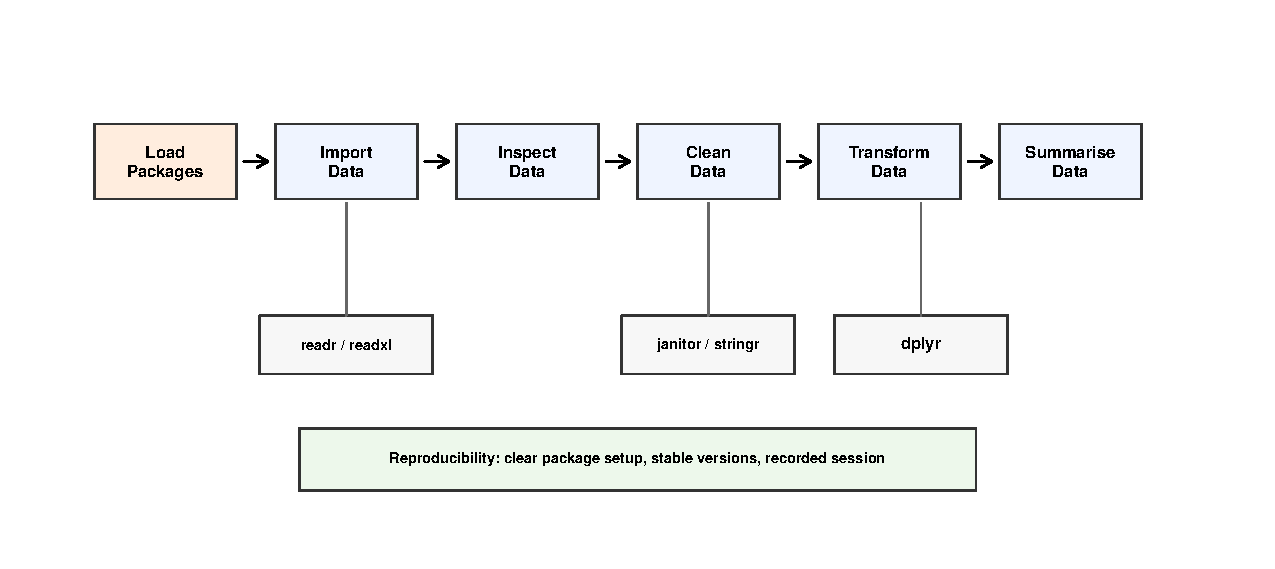
\includegraphics[width=0.9\linewidth,height=\textheight,keepaspectratio]{chapters/11-packages_files/figure-pdf/fig-package-workflow-map-1.pdf}

}

\caption{\label{fig-package-workflow-map}Packages Supporting Different
Stages of a Reproducible Workflow}

\end{figure}%

As shown in Figure~\ref{fig-package-workflow-map}, packages are not
random additions to R. Different packages support different stages of
the workflow. Some help data enter R. Some help clean or transform data.
Others help maintain reproducibility across the analysis process.

The movement of Part 3 will become:

\begin{Shaded}
\begin{Highlighting}[]
\NormalTok{Load tools.}
\NormalTok{Import data.}
\NormalTok{Inspect data.}
\NormalTok{Clean data.}
\NormalTok{Select and transform data.}
\NormalTok{Summarise and group data.}
\end{Highlighting}
\end{Shaded}

Packages are not the whole workflow.

They make the workflow possible.

\section{Common Beginner Mistakes}\label{common-beginner-mistakes-3}

Package problems are common because beginners often copy code from
tutorials without understanding the setup behind it.

Leo can avoid many problems by recognising a few patterns.

\subsection{Mistake 1: Installing a package every time a script
runs}\label{mistake-1-installing-a-package-every-time-a-script-runs}

A beginner may write this at the top of every script:

\begin{Shaded}
\begin{Highlighting}[]
\FunctionTok{install.packages}\NormalTok{(}\StringTok{"dplyr"}\NormalTok{)}
\FunctionTok{library}\NormalTok{(dplyr)}
\end{Highlighting}
\end{Shaded}

A cleaner daily analysis habit is usually:

\begin{Shaded}
\begin{Highlighting}[]
\FunctionTok{library}\NormalTok{(dplyr)}
\end{Highlighting}
\end{Shaded}

Install the package when the computer needs it. Load it when the session
needs it.

\subsection{Mistake 2: Loading a package before it is
installed}\label{mistake-2-loading-a-package-before-it-is-installed}

This will fail if \texttt{readxl} is not installed:

\begin{Shaded}
\begin{Highlighting}[]
\FunctionTok{library}\NormalTok{(readxl)}
\end{Highlighting}
\end{Shaded}

Install first:

\begin{Shaded}
\begin{Highlighting}[]
\FunctionTok{install.packages}\NormalTok{(}\StringTok{"readxl"}\NormalTok{)}
\end{Highlighting}
\end{Shaded}

Then load:

\begin{Shaded}
\begin{Highlighting}[]
\FunctionTok{library}\NormalTok{(readxl)}
\end{Highlighting}
\end{Shaded}

The order matters because R cannot open a toolbox that has not been
placed on the computer.

\subsection{\texorpdfstring{Mistake 3: Forgetting quotation marks in
\texttt{install.packages()}}{Mistake 3: Forgetting quotation marks in install.packages()}}\label{mistake-3-forgetting-quotation-marks-in-install.packages}

This is wrong:

\begin{Shaded}
\begin{Highlighting}[]
\FunctionTok{install.packages}\NormalTok{(dplyr)}
\end{Highlighting}
\end{Shaded}

This is correct:

\begin{Shaded}
\begin{Highlighting}[]
\FunctionTok{install.packages}\NormalTok{(}\StringTok{"dplyr"}\NormalTok{)}
\end{Highlighting}
\end{Shaded}

The package name is text, so it needs quotation marks.

\subsection{\texorpdfstring{Mistake 4: Putting quotation marks inside
\texttt{library()}
unnecessarily}{Mistake 4: Putting quotation marks inside library() unnecessarily}}\label{mistake-4-putting-quotation-marks-inside-library-unnecessarily}

This can work in many cases:

\begin{Shaded}
\begin{Highlighting}[]
\FunctionTok{library}\NormalTok{(}\StringTok{"dplyr"}\NormalTok{)}
\end{Highlighting}
\end{Shaded}

But the common style is:

\begin{Shaded}
\begin{Highlighting}[]
\FunctionTok{library}\NormalTok{(dplyr)}
\end{Highlighting}
\end{Shaded}

Leo should recognise both. In this book, the common style will be used.

\subsection{Mistake 5: Ignoring conflict
messages}\label{mistake-5-ignoring-conflict-messages}

Conflict messages are not decorations. They are information.

When Leo sees a conflict message, he should read it. If he is unsure
which function is being used, he can write:

\begin{Shaded}
\begin{Highlighting}[]
\NormalTok{dplyr}\SpecialCharTok{::}\FunctionTok{filter}\NormalTok{(df\_r\_migration, project\_score }\SpecialCharTok{\textgreater{}=} \DecValTok{80}\NormalTok{)}
\end{Highlighting}
\end{Shaded}

The namespace makes the source of the function clear.

\subsection{Mistake 6: Loading many packages without knowing
why}\label{mistake-6-loading-many-packages-without-knowing-why}

A script should not begin with a pile of packages copied from the
internet.

Each package should have a reason.

If Leo cannot explain why a package is loaded, he should pause before
adding it to the workflow.

\section{Try It Yourself}\label{try-it-yourself-2}

Try loading \texttt{dplyr}:

\begin{Shaded}
\begin{Highlighting}[]
\FunctionTok{library}\NormalTok{(dplyr)}
\end{Highlighting}
\end{Shaded}

If R says the package is missing, install it:

\begin{Shaded}
\begin{Highlighting}[]
\FunctionTok{install.packages}\NormalTok{(}\StringTok{"dplyr"}\NormalTok{)}
\FunctionTok{library}\NormalTok{(dplyr)}
\end{Highlighting}
\end{Shaded}

Then check the version:

\begin{Shaded}
\begin{Highlighting}[]
\FunctionTok{packageVersion}\NormalTok{(}\StringTok{"dplyr"}\NormalTok{)}
\end{Highlighting}
\end{Shaded}

Now use a function with an explicit namespace:

\begin{Shaded}
\begin{Highlighting}[]
\NormalTok{dplyr}\SpecialCharTok{::}\FunctionTok{select}\NormalTok{(df\_r\_migration, learner\_id, country, project\_score)}
\end{Highlighting}
\end{Shaded}

Reflect on these questions:

\begin{itemize}
\tightlist
\item
  Which action installs the package?
\item
  Which action loads the package?
\item
  What does \texttt{package::function()} make clear?
\item
  Why should a script not load packages without purpose?
\item
  Why might package versions matter in a research project?
\end{itemize}

The aim is not to memorise package commands. The aim is to understand
what each command is doing to the workflow.

\section{A Small Practice Lab}\label{a-small-practice-lab-3}

Create a package section:

\begin{Shaded}
\begin{Highlighting}[]
\CommentTok{\# Packages}
\FunctionTok{library}\NormalTok{(readr)}
\FunctionTok{library}\NormalTok{(dplyr)}
\end{Highlighting}
\end{Shaded}

Now write the same idea using namespaces:

\begin{Shaded}
\begin{Highlighting}[]
\NormalTok{raw\_migration }\OtherTok{\textless{}{-}}\NormalTok{ readr}\SpecialCharTok{::}\FunctionTok{read\_csv}\NormalTok{(}\StringTok{"data/raw/df\_r\_migration\_messy.csv"}\NormalTok{)}

\NormalTok{dplyr}\SpecialCharTok{::}\FunctionTok{glimpse}\NormalTok{(raw\_migration)}
\end{Highlighting}
\end{Shaded}

Compare the two styles.

Ask:

\begin{itemize}
\tightlist
\item
  Which is shorter?
\item
  Which is more explicit?
\item
  Which would be easier in a script that uses many \texttt{dplyr}
  functions?
\item
  Which would be clearer if only one function from a package is needed?
\end{itemize}

There is no single answer that fits every project.

The important point is that Leo now understands the difference between
convenience and explicitness.

\section{Short Recap}\label{short-recap-2}

Leo has learned that packages extend R by adding purposeful tools.

He has also learned that packages are not just names to copy from
tutorials. They belong to the discipline of workflow.

The main points are:

\begin{itemize}
\tightlist
\item
  base R already provides many useful tools;
\item
  external packages extend R for specific tasks;
\item
  installing and loading are different actions;
\item
  \texttt{install.packages()} stores a package on the computer;
\item
  \texttt{library()} opens a package for the current session;
\item
  package commands should usually appear in a clear setup section;
\item
  namespaces show where functions live;
\item
  function conflicts happen when names are shared;
\item
  \texttt{package::function()} can make code clearer;
\item
  documentation helps Leo investigate tools responsibly;
\item
  package versions matter for reproducibility.
\end{itemize}

The core idea is simple:

\begin{quote}
Packages extend R, but reproducible analysis depends on knowing which
tools are being used, where they come from, and when they enter the
workflow.
\end{quote}

That sentence is the lightbulb.

Leo is no longer just collecting tools. He is learning how to arrange
them deliberately inside a reproducible workflow.

\section{Leo's Notebook}\label{leos-notebook-5}

Leo writes:

\begin{quote}
In Chapter 2, I first met packages as specialist systems, like avionics.
Now I understand the practical side: each package is a specialist
toolbox. I should know which toolbox I am opening and why.
\end{quote}

He adds:

\begin{quote}
Installing a package and loading a package are not the same.
Installation puts the toolbox on my computer. Loading opens it for the
current session.
\end{quote}

Then he writes one more note:

\begin{quote}
When two tools have the same name, I can use
\texttt{package::function()} to tell R exactly which one I mean.
\end{quote}

He pauses after that final sentence.

It is not just a package lesson.

It is the beginning of workflow discipline.

\section{Glossary}\label{glossary-2}

\textbf{Package}\\
A collection of functions, documentation, data, and resources that
extends what R can do.

\textbf{Base R}\\
The core set of functions and tools available in a standard R
installation.

\textbf{External package}\\
A package that usually must be installed separately before it can be
used.

\textbf{Install}\\
To place a package on the computer so R can access it.

\textbf{Load}\\
To make a package available in the current R session.

\textbf{Session}\\
The current running instance of R.

\textbf{Namespace}\\
The space where a package keeps its functions and objects.

\textbf{Function conflict}\\
A situation where more than one package provides a function with the
same name.

\textbf{\texttt{package::function()}}\strut \\
A way to call a function from a specific package without ambiguity.

\textbf{Package version}\\
The specific release of a package being used.

\textbf{Reproducibility}\\
The ability to rerun an analysis and obtain the same or equivalent
result under a documented computational setup.

\section{Chapter Outcome}\label{chapter-outcome-10}

By the end of this chapter, Leo can:

\begin{itemize}
\tightlist
\item
  define an R package;
\item
  explain why packages exist;
\item
  distinguish base tools from external packages;
\item
  install a package;
\item
  load a package;
\item
  explain the difference between installing and loading;
\item
  recognise namespace syntax;
\item
  respond calmly to function conflicts;
\item
  use \texttt{package::function()} when clarity is needed;
\item
  connect package use to reproducible workflows;
\item
  understand why package documentation and versions matter.
\end{itemize}

These are not small skills.

They are the habits that help Leo move from writing commands that work
once to building workflows that other people can understand, rerun, and
trust.

\section{What Comes Next}\label{what-comes-next-4}

Leo now understands how R gains new tools.

But tools are not the data.

Before Leo can clean, transform, summarise, model, or visualise
anything, the data must enter R. That sounds simple until the first real
file appears.

A file can sit neatly in a project folder and still be unreadable to R.
A spreadsheet can look correct on the screen and still arrive with
broken column names. A date can look like a date to Leo and behave like
text inside R. A missing value can look blank in Excel and become
something else during import.

This is why importing is not merely opening a file. It is asking R to
interpret the file as data.

Chapter 12 begins at that threshold.

Leo now knows how to arrange the tools. Next, he must learn how to bring
data into R without mistaking a file on the screen for evidence R can
trust.

\chapter{Importing Data: From Files on Disk to Objects R Can Work
With}\label{importing-data-from-files-on-disk-to-objects-r-can-work-with}

\renewcommand{\thefigure}{12.\arabic{figure}}
\setcounter{figure}{0}
\renewcommand{\thetable}{12.\arabic{table}}
\setcounter{table}{0}

\section{Opening Scene: The File Leo Can See but R Cannot Yet
Use}\label{opening-scene-the-file-leo-can-see-but-r-cannot-yet-use}

Leo has just crossed an important threshold.

In Part 2, he learned how R speaks. He learned that code has structure,
that logic turns conditions into judgments, that built-in functions are
ready-made actions, and that repeated rules can be given names of their
own.

Then Part 3 began.

Chapter 11 showed him that serious R work does not depend on language
alone. A real workflow also needs tools. Some tools help R read files.
Some help inspect data. Some help clean names, work with dates, handle
text, transform columns, summarise groups, and record the computational
setup.

Now the tools are ready.

Leo looks inside the project folder and sees this file:

\begin{Shaded}
\begin{Highlighting}[]
\NormalTok{df\_r\_migration\_messy.csv}
\end{Highlighting}
\end{Shaded}

He can open it in a spreadsheet program. Rows and columns appear. He can
see learner IDs, countries, backgrounds, study hours, project scores,
completion status, dates, tool-use indicators, and notes.

It feels as if the data are already available.

But R cannot analyse a file simply because Leo can see it on the screen.

The file is still outside R. It is stored on disk. R needs to be told
where the file is, how to read it, and what object name should hold the
imported result.

That is the first serious lesson of this chapter:

\begin{quote}
Importing data is not just opening a file. It is the act of turning an
external file into an R object that must be located, read, inspected,
and verified before analysis.
\end{quote}

\begin{tcolorbox}[enhanced jigsaw, arc=.35mm, bottomrule=.15mm, breakable, colback=white, colframe=quarto-callout-note-color-frame, left=2mm, leftrule=.75mm, opacityback=0, rightrule=.15mm, toprule=.15mm]
\begin{minipage}[t]{5.5mm}
\textcolor{quarto-callout-note-color}{\faInfo}
\end{minipage}%
\begin{minipage}[t]{\textwidth - 5.5mm}

\vspace{-3mm}\textbf{Chapter Compass}\vspace{3mm}

In this chapter, Leo learns how to move data from a CSV file into R
without losing control of the workflow. He will learn the difference
between a file, a path, and an object; how to use project-relative
paths; how to import the official raw dataset; how to inspect what
arrived; and why importing data is not the same as trusting it.

This chapter does not teach full cleaning. That work begins in Chapter
13.

\end{minipage}%
\end{tcolorbox}

\section{What Changed After Chapter
11}\label{what-changed-after-chapter-11}

Chapter 11 prepared Leo's tools. It showed that packages are not random
add-ons. They are selected because a workflow needs them.

For this chapter, one package matters especially: \texttt{readr}. It
provides \texttt{read\_csv()}, a clear and modern way to import CSV
files into R. Base R can also import CSV files with \texttt{read.csv()}.
In this book's Part 3 workflow, Leo will mainly use
\texttt{readr::read\_csv()} because it gives clear import messages,
works well with the workflow tools introduced in Chapter 11, and fits
the book's movement toward reproducible analysis.

This book continues to use both Base R and tidyverse tools deliberately.
Base R helps explain how R works internally. Tidyverse tools help
express common workflow tasks clearly and consistently.

The Chapter 11 principle still holds:

\begin{quote}
Base R teaches the structure of the language. Tidyverse teaches workflow
fluency. Serious R users eventually understand both.
\end{quote}

In Chapter 12, the practical issue is simple: Leo needs a reliable way
to bring the official CSV file into R, inspect it, and keep the raw
evidence protected.

\section{The Part 3 Workflow So Far}\label{the-part-3-workflow-so-far}

Part 3 follows a practical workflow path:

\begin{Shaded}
\begin{Highlighting}[]
\NormalTok{Packages {-}\textgreater{} Import {-}\textgreater{} Inspect {-}\textgreater{} Clean {-}\textgreater{} Transform {-}\textgreater{} Summarise}
\end{Highlighting}
\end{Shaded}

Chapter 11 prepared the tools. Chapter 12 now handles the first data
movement: import.

The workflow has not reached cleaning yet. Leo is not correcting country
names, fixing date formats, recoding logical fields, or removing
duplicate records in this chapter. He is learning how to make the data
enter R in a way that can be checked.

That order matters. If the import is unclear, every later step becomes
fragile.

\section{The Official Dataset for This
Book}\label{the-official-dataset-for-this-book}

The official dataset for Part 3 is:

\begin{Shaded}
\begin{Highlighting}[]
\NormalTok{df\_r\_migration\_messy.csv}
\end{Highlighting}
\end{Shaded}

In the project workflow, the raw file should live here:

\begin{Shaded}
\begin{Highlighting}[]
\NormalTok{data/raw/df\_r\_migration\_messy.csv}
\end{Highlighting}
\end{Shaded}

To follow Leo's workflow on your own machine, download the raw teaching
dataset here:

\href{../data/raw/df_r_migration_messy.csv}{Download
\texttt{df\_r\_migration\_messy.csv}}

If a local preview opens the CSV in the browser because it is a
plain-text file, use your browser's \textbf{Save As} or \textbf{Save
Link As} option. In many published HTML versions, the download attribute
encourages the browser to treat the link as a downloadable file. If the
CSV still opens in a browser tab, use Save As or Save Link As to save it
locally.

The path used in the download link is for the rendered book. The path
used inside the R code below is the project-relative path R should
follow from the project root. Table~\ref{tbl-official-dataset-overview}
summarises the official raw dataset before Leo imports it.

\begin{longtable}[]{@{}
  >{\raggedright\arraybackslash}p{(\linewidth - 2\tabcolsep) * \real{0.5000}}
  >{\raggedright\arraybackslash}p{(\linewidth - 2\tabcolsep) * \real{0.5000}}@{}}
\caption{Overview of the official raw teaching
dataset}\label{tbl-official-dataset-overview}\tabularnewline
\toprule\noalign{}
\begin{minipage}[b]{\linewidth}\raggedright
Item
\end{minipage} & \begin{minipage}[b]{\linewidth}\raggedright
Detail
\end{minipage} \\
\midrule\noalign{}
\endfirsthead
\toprule\noalign{}
\begin{minipage}[b]{\linewidth}\raggedright
Item
\end{minipage} & \begin{minipage}[b]{\linewidth}\raggedright
Detail
\end{minipage} \\
\midrule\noalign{}
\endhead
\bottomrule\noalign{}
\endlastfoot
File name & \texttt{df\_r\_migration\_messy.csv} \\
File type & CSV file \\
Project location & \texttt{data/raw/df\_r\_migration\_messy.csv} \\
Rows & 650 \\
Columns & 28 \\
Unit of observation & One recorded learner observation within the R
migration learning journey \\
Purpose in the book & A deliberately messy raw dataset for teaching
import, inspection, cleaning, transformation, and summary \\
\end{longtable}

The dataset contains \texttt{650} rows and \texttt{28} columns. The
columns are:

\texttt{learner\_id}, \texttt{learner\_name}, \texttt{country},
\texttt{region}, \texttt{job\_role}, \texttt{industry},
\texttt{background}, \texttt{excel\_years},
\texttt{r\_experience\_level}, \texttt{enrolment\_date},
\texttt{first\_login\_date}, \texttt{week}, \texttt{study\_hours},
\texttt{lessons\_completed}, \texttt{confidence\_score},
\texttt{pre\_assessment\_score}, \texttt{project\_score},
\texttt{first\_script\_completed}, \texttt{used\_rstudio},
\texttt{used\_quarto}, \texttt{used\_git}, \texttt{used\_renv},
\texttt{preferred\_learning\_mode}, \texttt{monthly\_income\_band},
\texttt{completion\_status}, \texttt{manager\_support}, \texttt{notes},
\texttt{payment\_probability\_score}.

The dataset tells a simple learning story. The file follows learners
moving from spreadsheet-heavy or reporting-heavy backgrounds into
R-based data work. Each row should be read as a recorded learner
observation within that learning journey, not as a guarantee that every
learner appears only once. It records personal and learning-context
fields such as \texttt{learner\_id}, \texttt{country}, \texttt{region},
\texttt{job\_role}, \texttt{industry}, and \texttt{background}; progress
indicators such as \texttt{week}, \texttt{study\_hours},
\texttt{lessons\_completed}, \texttt{confidence\_score},
\texttt{pre\_assessment\_score}, and \texttt{project\_score}; tool-use
fields such as \texttt{used\_rstudio}, \texttt{used\_quarto},
\texttt{used\_git}, and \texttt{used\_renv}; and outcome or context
fields such as \texttt{completion\_status}, \texttt{manager\_support},
\texttt{notes}, and \texttt{payment\_probability\_score}.

The file is intentionally messy. That is not a flaw in the book. It is
the teaching engine for Part 3.

A perfectly clean teaching file would make import look easy, but it
would hide the work that real analysts actually face. Real datasets
often contain inconsistent capitalisation, extra spaces, missing-like
values, mixed date formats, duplicated identifiers, and values that look
suspicious only after careful inspection.

This file includes those kinds of problems. Initial inspection shows:

\begin{itemize}
\tightlist
\item
  text fields such as \texttt{country}, \texttt{industry},
  \texttt{background}, \texttt{job\_role}, and
  \texttt{completion\_status} contain inconsistent capitalisation or
  extra spaces;
\item
  logical fields such as \texttt{first\_script\_completed},
  \texttt{used\_rstudio}, \texttt{used\_quarto}, \texttt{used\_git},
  \texttt{used\_renv}, and \texttt{manager\_support} are encoded in
  several ways, including values such as \texttt{TRUE}, \texttt{FALSE},
  \texttt{Yes}, \texttt{No}, \texttt{Y}, \texttt{N}, \texttt{1}, and
  \texttt{0};
\item
  date fields such as \texttt{enrolment\_date} and
  \texttt{first\_login\_date} appear in more than one format;
\item
  missing-like values appear especially in \texttt{first\_login\_date},
  \texttt{confidence\_score}, \texttt{project\_score}, and
  \texttt{notes};
\item
  there are repeated learner IDs, and learner-week records will need
  careful checking later;
\item
  \texttt{study\_hours} includes a suspicious negative value that should
  not be ignored.
\end{itemize}

Chapter 12 does not fix those problems. It teaches Leo how to bring the
file into R and inspect what arrived. Chapter 13 will ask what to do
with the problems once they are visible.

\section{File, Path, and Object Are Not the Same
Thing}\label{file-path-and-object-are-not-the-same-thing}

Many importing problems begin with one small confusion: the learner sees
a file and assumes R can see it too.

R does not work from human eyesight. For file-based workflows, R works
from paths and objects.

\begin{longtable}[]{@{}
  >{\raggedright\arraybackslash}p{(\linewidth - 4\tabcolsep) * \real{0.3333}}
  >{\raggedright\arraybackslash}p{(\linewidth - 4\tabcolsep) * \real{0.3333}}
  >{\raggedright\arraybackslash}p{(\linewidth - 4\tabcolsep) * \real{0.3333}}@{}}
\caption{Common file, path, and object
distinctions}\label{tbl-file-path-object-distinction}\tabularnewline
\toprule\noalign{}
\begin{minipage}[b]{\linewidth}\raggedright
Concept
\end{minipage} & \begin{minipage}[b]{\linewidth}\raggedright
Meaning
\end{minipage} & \begin{minipage}[b]{\linewidth}\raggedright
Example
\end{minipage} \\
\midrule\noalign{}
\endfirsthead
\toprule\noalign{}
\begin{minipage}[b]{\linewidth}\raggedright
Concept
\end{minipage} & \begin{minipage}[b]{\linewidth}\raggedright
Meaning
\end{minipage} & \begin{minipage}[b]{\linewidth}\raggedright
Example
\end{minipage} \\
\midrule\noalign{}
\endhead
\bottomrule\noalign{}
\endlastfoot
File & The actual dataset stored on disk. &
\texttt{df\_r\_migration\_messy.csv} \\
Path & The address R follows to find the file. &
\texttt{data/raw/df\_r\_migration\_messy.csv} \\
Object & The version of the data R holds in memory after import. &
\texttt{raw\_migration} \\
\end{longtable}

The distinction in Table~\ref{tbl-file-path-object-distinction} is one
of the most important ideas in this chapter because many import errors
begin when these three ideas are treated as the same thing.

A \textbf{file} can sit in a folder without being available inside R.

A \textbf{path} tells R where to look for the file.

An \textbf{object} is created only after R reads the file and stores the
result in memory.

So when Leo writes this:

\begin{Shaded}
\begin{Highlighting}[]
\NormalTok{raw\_migration }\OtherTok{\textless{}{-}}\NormalTok{ readr}\SpecialCharTok{::}\FunctionTok{read\_csv}\NormalTok{(}\StringTok{"data/raw/df\_r\_migration\_messy.csv"}\NormalTok{)}
\end{Highlighting}
\end{Shaded}

three things are happening.

First, the quoted text gives R the path to the file. Second,
\texttt{readr::read\_csv()} reads the CSV file. Third, the assignment
operator \texttt{\textless{}-} stores the imported result as an object
called \texttt{raw\_migration}.

That object is what R can inspect, count, print, and later clean.

\section{A Small Visual Map of
Importing}\label{a-small-visual-map-of-importing}

The movement from file to object is easier to understand when Leo sees
the whole import chain at once.

\begin{figure}

\centering{

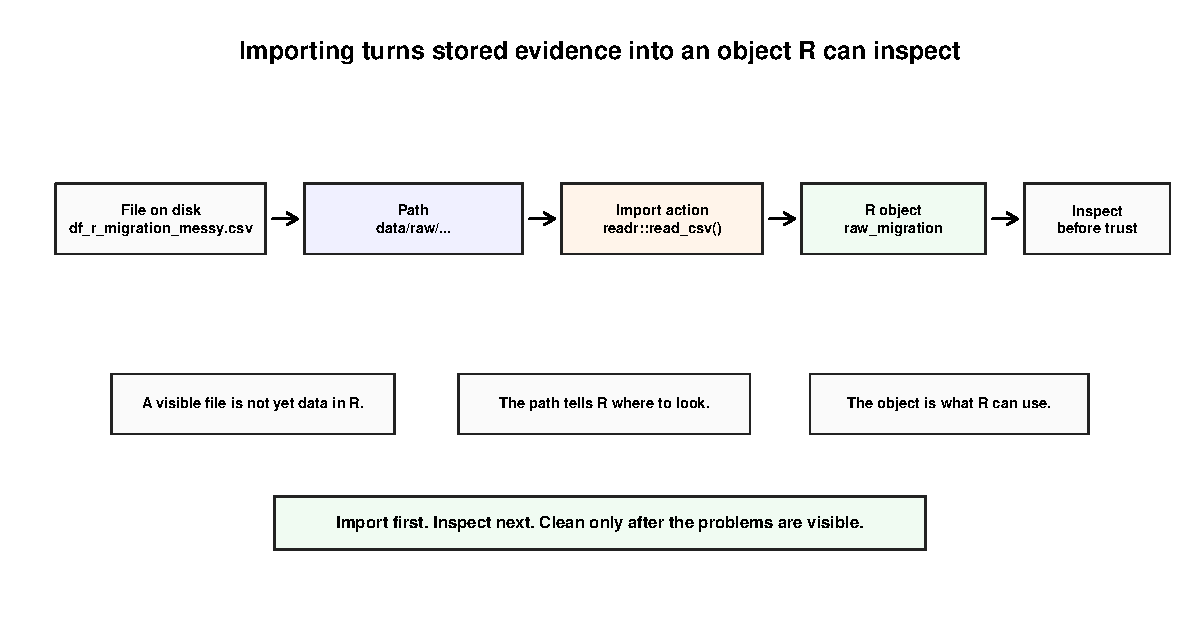
\includegraphics[width=0.9\linewidth,height=\textheight,keepaspectratio]{chapters/12-importing-data_files/figure-pdf/fig-file-path-object-import-1.pdf}

}

\caption{\label{fig-file-path-object-import}From File on Disk to Object
in R}

\end{figure}%

As shown in Figure~\ref{fig-file-path-object-import}, importing is a
controlled transition from external storage into R's working memory. The
important idea is not the function itself, but the sequence: locate the
file, import it deliberately, then verify what arrived before continuing
with analysis.

\section{Project-Relative Paths}\label{project-relative-paths}

Leo could import a file by writing a full path such as:

\begin{Shaded}
\begin{Highlighting}[]
\NormalTok{C:/Users/Leo/Documents/RBook/data/raw/df\_r\_migration\_messy.csv}
\end{Highlighting}
\end{Shaded}

That may work on Leo's computer, but it is a poor habit for a
reproducible project. The path is tied to one machine, one username, and
one folder arrangement.

A project-relative path is better:

\begin{Shaded}
\begin{Highlighting}[]
\NormalTok{data/raw/df\_r\_migration\_messy.csv}
\end{Highlighting}
\end{Shaded}

This path starts from the project root. It tells R to look inside the
project folder, then inside \texttt{data}, then inside \texttt{raw},
then for the CSV file.

That kind of path is easier to share, easier to render, and easier to
explain.

\begin{tcolorbox}[enhanced jigsaw, arc=.35mm, bottomrule=.15mm, breakable, colback=white, colframe=quarto-callout-tip-color-frame, left=2mm, leftrule=.75mm, opacityback=0, rightrule=.15mm, toprule=.15mm]
\begin{minipage}[t]{5.5mm}
\textcolor{quarto-callout-tip-color}{\faLightbulb}
\end{minipage}%
\begin{minipage}[t]{\textwidth - 5.5mm}

\vspace{-3mm}\textbf{Project Habit}\vspace{3mm}

Keep raw data inside the project, usually in a folder such as
\texttt{data/raw/}. Then refer to it with a project-relative path.

A path that works only on one computer is not a workflow. It is a local
accident waiting to happen.

\end{minipage}%
\end{tcolorbox}

Before importing, Leo can check whether the file exists:

\begin{Shaded}
\begin{Highlighting}[]
\FunctionTok{file.exists}\NormalTok{(}\StringTok{"data/raw/df\_r\_migration\_messy.csv"}\NormalTok{)}
\end{Highlighting}
\end{Shaded}

If R returns \texttt{TRUE}, the file is where the code expects it to be.
If R returns \texttt{FALSE}, Leo should not continue blindly. He should
check the file name, folder name, spelling, capitalisation, and working
directory.

\section{Importing the CSV File}\label{importing-the-csv-file}

The main import code for this chapter is short. In the rendered book,
some import chunks are shown without being evaluated so that the chapter
can render safely even before a reader has copied the dataset into the
project folder.

\begin{Shaded}
\begin{Highlighting}[]
\NormalTok{raw\_migration }\OtherTok{\textless{}{-}}\NormalTok{ readr}\SpecialCharTok{::}\FunctionTok{read\_csv}\NormalTok{(}\StringTok{"data/raw/df\_r\_migration\_messy.csv"}\NormalTok{)}
\end{Highlighting}
\end{Shaded}

This line should be read slowly.

\texttt{readr::read\_csv()} is the import function. The path inside
quotation marks tells R where the file is. The object name
\texttt{raw\_migration} tells R where to store the imported result.

The name \texttt{raw\_migration} is intentional. It reminds Leo that
this is the raw import, not a cleaned analysis dataset.

A beginner may be tempted to call the object \texttt{df\_r\_migration}
immediately. That is not wrong by itself, but this book keeps the first
imported object visibly raw. Later, Chapter 13 will create a working
copy for cleaning.

\begin{Shaded}
\begin{Highlighting}[]
\NormalTok{raw\_migration }\OtherTok{\textless{}{-}}\NormalTok{ readr}\SpecialCharTok{::}\FunctionTok{read\_csv}\NormalTok{(}\StringTok{"data/raw/df\_r\_migration\_messy.csv"}\NormalTok{)}

\CommentTok{\# Later, when cleaning begins:}
\NormalTok{df\_r\_migration }\OtherTok{\textless{}{-}}\NormalTok{ raw\_migration}
\end{Highlighting}
\end{Shaded}

The second line is shown only as a preview. In Chapter 13,
\texttt{df\_r\_migration} becomes the working copy used for cleaning and
preparation, while \texttt{raw\_migration} remains the untouched
imported evidence. Chapter 12 imports and inspects. Chapter 13 decides
what to change.

\section{A Base R Import Option}\label{a-base-r-import-option}

Base R can also import CSV files:

\begin{Shaded}
\begin{Highlighting}[]
\NormalTok{raw\_migration\_base }\OtherTok{\textless{}{-}} \FunctionTok{read.csv}\NormalTok{(}\StringTok{"data/raw/df\_r\_migration\_messy.csv"}\NormalTok{)}
\end{Highlighting}
\end{Shaded}

This is useful to know because Base R is always available with R.

In this book's Part 3 workflow, however, Leo will mainly use
\texttt{readr::read\_csv()} for the official dataset. That choice is
about consistent workflow practice, not about declaring one approach
superior. Base R helps Leo understand R's structure. The tidyverse
family helps him express common data-workflow steps clearly.

\section{Seeing What Came In}\label{seeing-what-came-in}

After importing, Leo should inspect the object immediately.

A common beginner mistake is to import a file and then rush into
analysis. That is risky. The file may have imported with unexpected
column types, missing values, date problems, strange column names,
duplicated IDs, or values that should not be possible.

The first inspection can be simple:

\begin{Shaded}
\begin{Highlighting}[]
\FunctionTok{names}\NormalTok{(raw\_migration)}
\end{Highlighting}
\end{Shaded}

\begin{Shaded}
\begin{Highlighting}[]
\FunctionTok{dim}\NormalTok{(raw\_migration)}
\end{Highlighting}
\end{Shaded}

\begin{Shaded}
\begin{Highlighting}[]
\FunctionTok{str}\NormalTok{(raw\_migration)}
\end{Highlighting}
\end{Shaded}

\begin{Shaded}
\begin{Highlighting}[]
\FunctionTok{head}\NormalTok{(raw\_migration)}
\end{Highlighting}
\end{Shaded}

These functions ask different inspection questions.

\texttt{names()} asks: what are the column names?

\texttt{dim()} asks: how many rows and columns arrived?

\texttt{str()} asks: what is the internal structure of the object?

\texttt{head()} asks: what do the first few rows look like?

Leo should not expect these checks to solve the data problems. Their
purpose is to reveal how R interpreted the file.

\section{Inspecting the Official
Dataset}\label{inspecting-the-official-dataset}

When Leo imports the CSV and inspects the resulting object,
\texttt{raw\_migration}, several things should become clear.

First, the dataset has \texttt{650} rows and \texttt{28} columns. If his
import returns a very different shape, something has gone wrong.

Second, the column names should match the official list. A missing
column or a strange extra column may suggest a file problem, an import
problem, or an accidental edit.

Third, the data should still look raw. That is expected. Raw data are
expected to contain inconsistencies. The analyst's responsibility is to
inspect them before analysis begins.

Here are the checks Leo should run after import:

\begin{Shaded}
\begin{Highlighting}[]
\FunctionTok{dim}\NormalTok{(raw\_migration)}
\FunctionTok{names}\NormalTok{(raw\_migration)}
\end{Highlighting}
\end{Shaded}

He can also inspect selected columns without cleaning them:

\begin{Shaded}
\begin{Highlighting}[]
\FunctionTok{unique}\NormalTok{(raw\_migration}\SpecialCharTok{$}\NormalTok{completion\_status)}
\FunctionTok{unique}\NormalTok{(raw\_migration}\SpecialCharTok{$}\NormalTok{first\_script\_completed)}
\FunctionTok{head}\NormalTok{(raw\_migration}\SpecialCharTok{$}\NormalTok{enrolment\_date)}
\FunctionTok{summary}\NormalTok{(raw\_migration}\SpecialCharTok{$}\NormalTok{study\_hours)}
\end{Highlighting}
\end{Shaded}

These lines are not cleaning steps. They are questions. They help Leo
see why Chapter 13 will be necessary.

\section{Import Messages Are Part of the
Evidence}\label{import-messages-are-part-of-the-evidence}

When \texttt{readr::read\_csv()} imports a file, it often reports what
it found. It may show how many rows and columns were read. It may
describe column types. It may tell Leo whether the parser made
assumptions.

Beginners sometimes ignore those messages because they look technical.
That is understandable, but it is not a good professional habit.

Import messages are not decoration. They are early evidence about how R
interpreted the file.

If R says a date column came in as character, Leo should notice. If R
says a score column came in as character, he should pause. If the number
of rows or columns does not match expectation, he should stop and
investigate.

\begin{tcolorbox}[enhanced jigsaw, arc=.35mm, bottomrule=.15mm, breakable, colback=white, colframe=quarto-callout-important-color-frame, left=2mm, leftrule=.75mm, opacityback=0, rightrule=.15mm, toprule=.15mm]
\begin{minipage}[t]{5.5mm}
\textcolor{quarto-callout-important-color}{\faExclamation}
\end{minipage}%
\begin{minipage}[t]{\textwidth - 5.5mm}

\vspace{-3mm}\textbf{Reliable Analysis Rule}\vspace{3mm}

Importing is not verification. A file becomes useful only after R reads
it and the analyst inspects what came in.

\end{minipage}%
\end{tcolorbox}

\section{Protecting the Raw Data}\label{protecting-the-raw-data}

The file in \texttt{data/raw/} should be treated as evidence.

Leo should not open the raw CSV in a spreadsheet program, edit cells
manually, save the file again, and then continue as if nothing changed.
That breaks the trail between the original file and the analysis.

A better workflow is:

\begin{Shaded}
\begin{Highlighting}[]
\NormalTok{data/raw/       original raw file}
\NormalTok{data/processed/ cleaned or prepared version}
\end{Highlighting}
\end{Shaded}

Chapter 12 is concerned with \texttt{data/raw/}. Chapter 13 will create
a cleaned or prepared result later.

For now, Leo should keep the rule simple:

\begin{quote}
Raw data should be imported and inspected, not manually edited into
silence.
\end{quote}

\section{Common Beginner Mistakes}\label{common-beginner-mistakes-4}

\subsection{Mistake 1: Confusing the file name with the object
name}\label{mistake-1-confusing-the-file-name-with-the-object-name}

The file is called:

\begin{Shaded}
\begin{Highlighting}[]
\NormalTok{df\_r\_migration\_messy.csv}
\end{Highlighting}
\end{Shaded}

The imported object may be called:

\begin{Shaded}
\begin{Highlighting}[]
\NormalTok{raw\_migration}
\end{Highlighting}
\end{Shaded}

Those are not the same thing.

The file sits on disk. The object lives inside R after import.

\subsection{Mistake 2: Forgetting quotation marks around the
path}\label{mistake-2-forgetting-quotation-marks-around-the-path}

This will not work:

\begin{Shaded}
\begin{Highlighting}[]
\NormalTok{readr}\SpecialCharTok{::}\FunctionTok{read\_csv}\NormalTok{(data}\SpecialCharTok{/}\NormalTok{raw}\SpecialCharTok{/}\NormalTok{df\_r\_migration\_messy.csv)}
\end{Highlighting}
\end{Shaded}

R needs the path as text:

\begin{Shaded}
\begin{Highlighting}[]
\NormalTok{readr}\SpecialCharTok{::}\FunctionTok{read\_csv}\NormalTok{(}\StringTok{"data/raw/df\_r\_migration\_messy.csv"}\NormalTok{)}
\end{Highlighting}
\end{Shaded}

The quotation marks tell R that the path is a character value, not a set
of object names and operators.

\subsection{Mistake 3: Using an absolute
path}\label{mistake-3-using-an-absolute-path}

This may work on one computer:

\begin{Shaded}
\begin{Highlighting}[]
\NormalTok{C:/Users/Leo/Downloads/df\_r\_migration\_messy.csv}
\end{Highlighting}
\end{Shaded}

But it will usually fail somewhere else.

Project-relative paths make a workflow more portable.

\subsection{Mistake 4: Importing from the Downloads
folder}\label{mistake-4-importing-from-the-downloads-folder}

The Downloads folder is temporary storage, not a reproducible project
structure. Before importing, move the file into the project, preferably:

\begin{Shaded}
\begin{Highlighting}[]
\NormalTok{data/raw/df\_r\_migration\_messy.csv}
\end{Highlighting}
\end{Shaded}

\subsection{Mistake 5: Assuming import means
clean}\label{mistake-5-assuming-import-means-clean}

Importing only brings the file into R. It does not standardise text,
repair dates, recode logical values, remove duplicates, or explain
suspicious values.

Those are later tasks.

\subsection{Mistake 6: Overwriting the raw
file}\label{mistake-6-overwriting-the-raw-file}

The raw file should remain untouched. If Leo creates a cleaned version
later, it should be saved separately.

\section{What Leo Is Expected to Know at This
Point}\label{what-leo-is-expected-to-know-at-this-point-5}

By the end of this chapter, Leo should be able to explain the import
workflow in plain language.

He should know that a file on disk is not the same as an object in R. He
should understand that a path is how R finds a file. He should be able
to import the official CSV with a project-relative path. He should know
why the first imported object is called \texttt{raw\_migration}. Most
importantly, he should know that inspection comes before trust.

\begin{tcolorbox}[enhanced jigsaw, arc=.35mm, bottomrule=.15mm, breakable, colback=white, colframe=quarto-callout-note-color-frame, left=2mm, leftrule=.75mm, opacityback=0, rightrule=.15mm, toprule=.15mm]
\begin{minipage}[t]{5.5mm}
\textcolor{quarto-callout-note-color}{\faInfo}
\end{minipage}%
\begin{minipage}[t]{\textwidth - 5.5mm}

\vspace{-3mm}\textbf{Not Yet}\vspace{3mm}

Leo is not expected to clean the dataset yet. He is not expected to fix
dates, recode categories, standardise text, remove duplicates, or decide
what to do with suspicious values.

Those tasks belong to Chapter 13. Chapter 12 ends once Leo knows how to
bring the raw file into R and inspect its condition before cleaning
begins.

\end{minipage}%
\end{tcolorbox}

\section{Chapter Outcome}\label{chapter-outcome-11}

Chapter 12 has moved Leo from tool preparation to data entry.

He now understands that importing data is a controlled movement:

\begin{Shaded}
\begin{Highlighting}[]
\NormalTok{file on disk {-}\textgreater{} path {-}\textgreater{} import function {-}\textgreater{} R object {-}\textgreater{} inspection}
\end{Highlighting}
\end{Shaded}

That movement is small, but it changes the workflow. Data is no longer
something Leo merely sees in a file. It is now something R can hold,
inspect, and prepare for the next stage.

The official raw dataset, \texttt{df\_r\_migration\_messy.csv}, has
entered the book's workflow. It is deliberately imperfect, which makes
it useful for learning. It will give Leo realistic practice with messy
categories, missing-like values, varied dates, mixed logical encodings,
duplicate identifiers, and suspicious numeric values.

But he should not repair those issues yet.

First he had to bring the evidence into R without damaging it.

That workflow step is now clear.

\section{Transition to Chapter 13}\label{transition-to-chapter-13}

The import step has revealed enough to make the next chapter necessary.

Leo can see the object. He can inspect its names, dimensions, structure,
and first rows. He can see signs of inconsistent text, missing values,
mixed date formats, repeated learner IDs, and suspicious values.

Now the harder question begins:

\begin{quote}
What should Leo do when the imported data are inconsistent, incomplete,
duplicated, or suspicious?
\end{quote}

\begin{tcolorbox}[enhanced jigsaw, arc=.35mm, bottomrule=.15mm, breakable, colback=white, colframe=quarto-callout-tip-color-frame, left=2mm, leftrule=.75mm, opacityback=0, rightrule=.15mm, toprule=.15mm]
\begin{minipage}[t]{5.5mm}
\textcolor{quarto-callout-tip-color}{\faLightbulb}
\end{minipage}%
\begin{minipage}[t]{\textwidth - 5.5mm}

\vspace{-3mm}\textbf{Ready for Cleaning}\vspace{3mm}

Leo can now bring the raw dataset into R and inspect what arrived.
Chapter 13 begins the next stage: cleaning and preparing the evidence
without hiding what changed.

\end{minipage}%
\end{tcolorbox}

\chapter{Cleaning and Preparing Data: Making Evidence
Trustworthy}\label{cleaning-and-preparing-data-making-evidence-trustworthy}

\renewcommand{\thefigure}{13.\arabic{figure}}
\setcounter{figure}{0}
\renewcommand{\thetable}{13.\arabic{table}}
\setcounter{table}{0}

\section{Opening Scene: When Import Reveals the
Work}\label{opening-scene-when-import-reveals-the-work}

Leo has done what many beginners think is the difficult part.

He has learned how to bring the CSV file into R.

In Chapter 12, the official raw dataset was brought into the workflow as
an object called \texttt{raw\_migration}. In the book's workflow, that
object represents the imported evidence. Leo can inspect its names,
dimensions, structure, and first rows before deciding what needs
attention.

That feels like progress, and it is.

But it is not yet analysis.

The moment a dataset enters R, a more serious question begins:

\begin{quote}
What condition is this evidence in?
\end{quote}

The answer is rarely perfect. Some values may be missing. Some
categories may be spelt or spaced differently. Some logical fields may
use \texttt{TRUE} and \texttt{FALSE}, while others use \texttt{Yes},
\texttt{No}, \texttt{Y}, \texttt{N}, \texttt{1}, and \texttt{0}. Some
dates may arrive in more than one format. Some numbers may look
suspicious. Some records may be repeated for good reasons, while others
may need investigation.

This is where beginners are often tempted to rush. They see a messy
column and immediately want to fix it. They see a missing value and
immediately want to replace it. They see a repeated ID and immediately
want to delete it.

That instinct is understandable, but it is risky.

Cleaning is not about making data look neat as quickly as possible. It
is about making the condition of the data explicit, consistent, and safe
enough for analysis without hiding what was changed.

\begin{tcolorbox}[enhanced jigsaw, arc=.35mm, bottomrule=.15mm, breakable, colback=white, colframe=quarto-callout-note-color-frame, left=2mm, leftrule=.75mm, opacityback=0, rightrule=.15mm, toprule=.15mm]
\begin{minipage}[t]{5.5mm}
\textcolor{quarto-callout-note-color}{\faInfo}
\end{minipage}%
\begin{minipage}[t]{\textwidth - 5.5mm}

\vspace{-3mm}\textbf{Chapter Compass}\vspace{3mm}

In this chapter, Leo learns how to prepare the imported evidence for
later analysis. He will keep the raw import untouched, create a working
copy, inspect the main forms of messiness, apply selected cleaning
steps, compare before and after, and record what changed.

This chapter does not teach full transformation. Chapter 14 will handle
selecting, filtering, and transforming data for analytical questions.

\end{minipage}%
\end{tcolorbox}

\section{What Changed After Chapter
12}\label{what-changed-after-chapter-12}

Chapter 12 taught Leo that a file, a path, and an object are not the
same thing.

The official CSV file lives in the project at:

\begin{Shaded}
\begin{Highlighting}[]
\NormalTok{data/raw/df\_r\_migration\_messy.csv}
\end{Highlighting}
\end{Shaded}

After import, the object created in R is:

\begin{Shaded}
\begin{Highlighting}[]
\NormalTok{raw\_migration}
\end{Highlighting}
\end{Shaded}

That object represents the raw imported evidence. Chapter 13 begins by
creating a working copy:

\begin{Shaded}
\begin{Highlighting}[]
\NormalTok{df\_r\_migration }\OtherTok{\textless{}{-}}\NormalTok{ raw\_migration}
\end{Highlighting}
\end{Shaded}

The distinction matters.

\texttt{raw\_migration} should remain the untouched import. Leo can
always return to it if he needs to check what the data looked like
before preparation.

\texttt{df\_r\_migration} is the working copy. This is where cleaning
and preparation happen.

\begin{Shaded}
\begin{Highlighting}[]
\NormalTok{df\_r\_migration }\OtherTok{\textless{}{-}}\NormalTok{ raw\_migration}
\end{Highlighting}
\end{Shaded}

If this chapter is rendered independently, Leo may need to recreate
\texttt{raw\_migration} from the official raw CSV before making the
working copy:

\begin{Shaded}
\begin{Highlighting}[]
\CommentTok{\# This setup is only for running Chapter 13 independently.}
\CommentTok{\# The learning workflow still continues from Chapter 12.}
\NormalTok{raw\_migration }\OtherTok{\textless{}{-}}\NormalTok{ readr}\SpecialCharTok{::}\FunctionTok{read\_csv}\NormalTok{(}\StringTok{"data/raw/df\_r\_migration\_messy.csv"}\NormalTok{)}

\NormalTok{df\_r\_migration }\OtherTok{\textless{}{-}}\NormalTok{ raw\_migration}
\end{Highlighting}
\end{Shaded}

The point is not to reteach importing. The point is to keep the evidence
trail clear:

\begin{Shaded}
\begin{Highlighting}[]
\NormalTok{raw import {-}\textgreater{} working copy {-}\textgreater{} prepared dataset}
\end{Highlighting}
\end{Shaded}

\section{The Part 3 Workflow So Far}\label{the-part-3-workflow-so-far-1}

Part 3 follows this workflow path:

\begin{Shaded}
\begin{Highlighting}[]
\NormalTok{Packages {-}\textgreater{} Import {-}\textgreater{} Inspect {-}\textgreater{} Clean {-}\textgreater{} Transform {-}\textgreater{} Summarise}
\end{Highlighting}
\end{Shaded}

Chapter 11 prepared the tools. Chapter 12 imported the official raw
dataset and inspected what arrived. Chapter 13 now begins the cleaning
and preparation stage.

This is also where Part 2 starts to pay off in practical work.

Chapter 6 taught Leo to read code as structure. Cleaning code must also
be structured clearly.

Chapter 7 taught him that logical judgments matter. Cleaning depends on
checks such as \texttt{is.na()}, \texttt{duplicated()},
\texttt{study\_hours\ \textless{}\ 0}, and
\texttt{first\_script\_completed\ \%in\%\ c("Yes",\ "Y",\ "1")}.

Chapter 8 taught him that built-in functions are ready-made actions.
Cleaning uses many of them: \texttt{names()}, \texttt{str()},
\texttt{summary()}, \texttt{is.na()}, \texttt{unique()},
\texttt{table()}, \texttt{trimws()}, \texttt{tolower()}, and
\texttt{colSums()}.

Chapter 9 taught him that repeated rules can be named. In this chapter,
Leo will see repeated cleaning patterns. Some are shown directly. Later,
those patterns could become small helper functions.

Part 3 is not a new unrelated beginning. It is Part 2 applied to real
data work.

\section{Raw Evidence and Working
Copy}\label{raw-evidence-and-working-copy}

The safest cleaning workflow begins with restraint.

Leo should not casually edit the raw import. He should first create a
working copy.

\begin{Shaded}
\begin{Highlighting}[]
\NormalTok{df\_r\_migration }\OtherTok{\textless{}{-}}\NormalTok{ raw\_migration}
\end{Highlighting}
\end{Shaded}

This line is small, but the habit is large.

The raw object answers the question:

\begin{quote}
What did R import from the official CSV?
\end{quote}

The working copy answers the question:

\begin{quote}
What version will Leo prepare for analysis?
\end{quote}

\begin{tcolorbox}[enhanced jigsaw, arc=.35mm, bottomrule=.15mm, breakable, colback=white, colframe=quarto-callout-important-color-frame, left=2mm, leftrule=.75mm, opacityback=0, rightrule=.15mm, toprule=.15mm]
\begin{minipage}[t]{5.5mm}
\textcolor{quarto-callout-important-color}{\faExclamation}
\end{minipage}%
\begin{minipage}[t]{\textwidth - 5.5mm}

\vspace{-3mm}\textbf{Reliable Analysis Rule}\vspace{3mm}

Do not clean the only copy of the evidence. Keep \texttt{raw\_migration}
untouched and use \texttt{df\_r\_migration} as the working copy.

\end{minipage}%
\end{tcolorbox}

That rule gives Leo room to make careful decisions. If a cleaning step
behaves unexpectedly, he can compare the working copy against the raw
import. If a reviewer asks what changed, he has a clearer trail. If a
mistake appears later, the original imported evidence is still
available.

\section{A Small Visual Map of
Cleaning}\label{a-small-visual-map-of-cleaning}

The cleaning workflow is easier to understand when the evidence trail is
visible.

\begin{figure}

\centering{

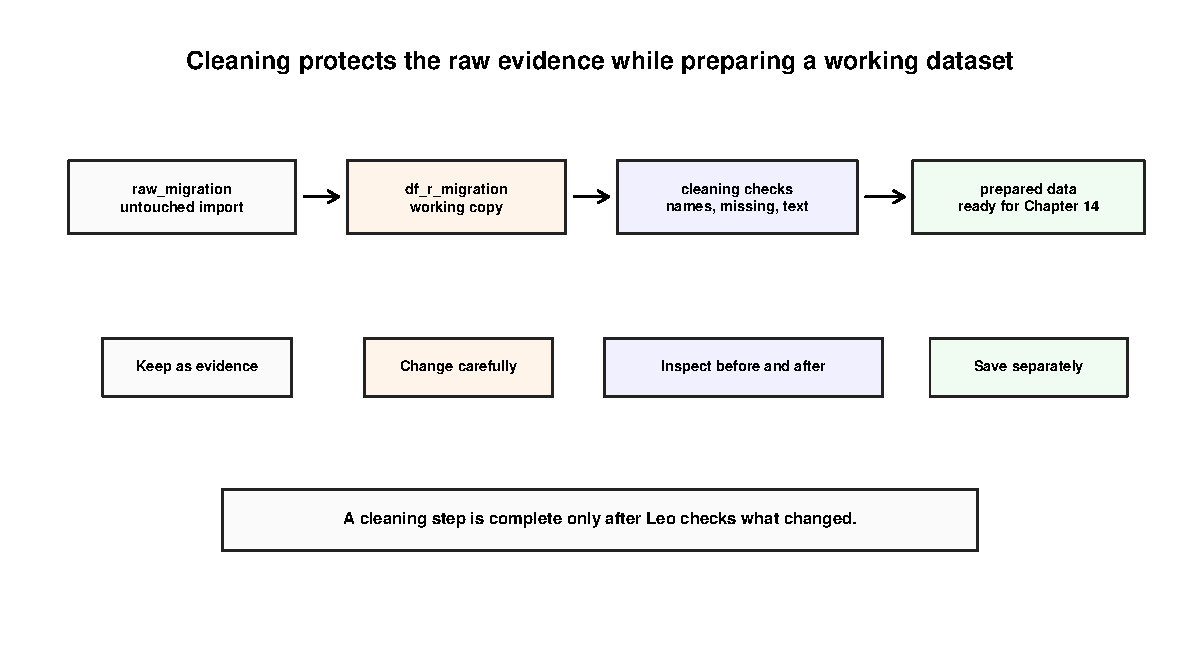
\includegraphics[width=0.9\linewidth,height=\textheight,keepaspectratio]{chapters/13-cleaning-and-preparing-data_files/figure-pdf/fig-raw-to-working-cleaning-1.pdf}

}

\caption{\label{fig-raw-to-working-cleaning}From Raw Evidence to a
Prepared Working Dataset}

\end{figure}%

As shown in Figure~\ref{fig-raw-to-working-cleaning}, cleaning should
not overwrite the raw evidence. The raw import remains available as
\texttt{raw\_migration}. The working copy, \texttt{df\_r\_migration},
carries the preparation work. Only after checks and documented decisions
should Leo create a prepared dataset for later analysis.

This is a professional habit, not an advanced trick.

\section{Before Cleaning: Inspect the
Mess}\label{before-cleaning-inspect-the-mess}

Chapter 12 made the condition of the official dataset visible. Chapter
13 now examines that condition more deliberately before changing
anything.

The dataset has 650 rows and 28 columns. It records learner observations
from people moving into R-based data work. It includes fields about
identity, background, dates, progress, tool use, completion, notes, and
payment probability.

The dataset is deliberately messy because real workflow practice needs
realistic evidence. Table~\ref{tbl-cleaning-issues} summarises the main
issues Leo should inspect before changing anything.

\begin{longtable}[]{@{}
  >{\raggedright\arraybackslash}p{(\linewidth - 4\tabcolsep) * \real{0.3333}}
  >{\raggedright\arraybackslash}p{(\linewidth - 4\tabcolsep) * \real{0.3333}}
  >{\raggedright\arraybackslash}p{(\linewidth - 4\tabcolsep) * \real{0.3333}}@{}}
\caption{Cleaning issues to inspect in the official
dataset}\label{tbl-cleaning-issues}\tabularnewline
\toprule\noalign{}
\begin{minipage}[b]{\linewidth}\raggedright
Cleaning issue
\end{minipage} & \begin{minipage}[b]{\linewidth}\raggedright
Variables to inspect
\end{minipage} & \begin{minipage}[b]{\linewidth}\raggedright
Why it matters
\end{minipage} \\
\midrule\noalign{}
\endfirsthead
\toprule\noalign{}
\begin{minipage}[b]{\linewidth}\raggedright
Cleaning issue
\end{minipage} & \begin{minipage}[b]{\linewidth}\raggedright
Variables to inspect
\end{minipage} & \begin{minipage}[b]{\linewidth}\raggedright
Why it matters
\end{minipage} \\
\midrule\noalign{}
\endhead
\bottomrule\noalign{}
\endlastfoot
Inconsistent text & \texttt{country}, \texttt{industry},
\texttt{background}, \texttt{job\_role}, \texttt{completion\_status} &
Grouping and counting become unreliable when the same category appears
in several forms. \\
Mixed logical encodings & \texttt{first\_script\_completed},
\texttt{used\_rstudio}, \texttt{used\_quarto}, \texttt{used\_git},
\texttt{used\_renv}, \texttt{manager\_support} & R may treat yes/no
fields as text unless the values are prepared consistently. \\
Varied date formats & \texttt{enrolment\_date},
\texttt{first\_login\_date} & Time-based work becomes unreliable when
dates are not recognised consistently. \\
Missing-like values & \texttt{first\_login\_date},
\texttt{confidence\_score}, \texttt{project\_score}, \texttt{notes} &
Missingness affects interpretation and should not be ignored. \\
Repeated records & \texttt{learner\_id}, \texttt{week} & Some repetition
may be valid, while repeated learner-week records require checking. \\
Suspicious numeric values & \texttt{study\_hours},
\texttt{project\_score}, \texttt{payment\_probability\_score} &
Impossible or unlikely values require investigation before analysis. \\
\end{longtable}

The table is not a cleaning recipe. It is an inspection map.

Leo should not remove records, replace values, or standardise categories
simply because a table says they look messy. Each cleaning step needs a
reason.

\section{Cleaning Is Not
Transformation}\label{cleaning-is-not-transformation}

Cleaning and transformation are related, but they are not the same job.

Cleaning prepares evidence so that the values are consistent enough to
interpret. It asks questions such as:

\begin{Shaded}
\begin{Highlighting}[]
\NormalTok{Are missing values marked consistently?}
\NormalTok{Are categories written consistently?}
\NormalTok{Are yes/no fields encoded consistently?}
\NormalTok{Are dates recognisable as dates?}
\NormalTok{Are there impossible or suspicious values?}
\NormalTok{Are repeated records valid or accidental?}
\end{Highlighting}
\end{Shaded}

Transformation creates or reshapes analytical meaning. It asks questions
such as:

\begin{Shaded}
\begin{Highlighting}[]
\NormalTok{Which columns do I need?}
\NormalTok{Which rows answer this question?}
\NormalTok{What new variable should I create?}
\NormalTok{How should this dataset be shaped for analysis?}
\end{Highlighting}
\end{Shaded}

Chapter 13 is about cleaning and preparation. Chapter 14 will teach Leo
how to select, filter, and transform data for analytical questions.

\begin{tcolorbox}[enhanced jigsaw, arc=.35mm, bottomrule=.15mm, breakable, colback=white, colframe=quarto-callout-note-color-frame, left=2mm, leftrule=.75mm, opacityback=0, rightrule=.15mm, toprule=.15mm]
\begin{minipage}[t]{5.5mm}
\textcolor{quarto-callout-note-color}{\faInfo}
\end{minipage}%
\begin{minipage}[t]{\textwidth - 5.5mm}

\vspace{-3mm}\textbf{Boundary Check}\vspace{3mm}

Cleaning makes existing evidence safer to work with. Transformation
reshapes or extends that evidence for a question.

Chapter 13 prepares. Chapter 14 transforms.

\end{minipage}%
\end{tcolorbox}

\section{Start with Column Names and
Structure}\label{start-with-column-names-and-structure}

Before changing values, Leo should inspect the structure.

Base R makes the first checks plain:

\begin{Shaded}
\begin{Highlighting}[]
\FunctionTok{names}\NormalTok{(df\_r\_migration)}
\FunctionTok{dim}\NormalTok{(df\_r\_migration)}
\FunctionTok{str}\NormalTok{(df\_r\_migration)}
\end{Highlighting}
\end{Shaded}

The tidyverse gives a compact structural view:

\begin{Shaded}
\begin{Highlighting}[]
\NormalTok{dplyr}\SpecialCharTok{::}\FunctionTok{glimpse}\NormalTok{(df\_r\_migration)}
\end{Highlighting}
\end{Shaded}

The official dataset already uses clear snake-case column names, such as
\texttt{learner\_id}, \texttt{study\_hours}, \texttt{project\_score},
and \texttt{completion\_status}. That is useful. It means Leo does not
need to begin by renaming columns.

But he should still inspect them.

A column name can look clean while the values inside the column remain
messy. That is why Chapter 13 moves from structure to values.

\begin{tcolorbox}[enhanced jigsaw, arc=.35mm, bottomrule=.15mm, breakable, colback=white, colframe=quarto-callout-tip-color-frame, left=2mm, leftrule=.75mm, opacityback=0, rightrule=.15mm, toprule=.15mm]
\begin{minipage}[t]{5.5mm}
\textcolor{quarto-callout-tip-color}{\faLightbulb}
\end{minipage}%
\begin{minipage}[t]{\textwidth - 5.5mm}

\vspace{-3mm}\textbf{Part 2 in Practice}\vspace{3mm}

Chapter 6 taught Leo to read code structurally. Chapter 13 asks him to
read data structurally too: names, rows, columns, types, and values all
have roles in the workflow.

\end{minipage}%
\end{tcolorbox}

\section{Missing Values and Missing-Like
Values}\label{missing-values-and-missing-like-values}

Missing values are not empty inconveniences. They are information about
absence, uncertainty, or non-response.

In the official dataset, missing-like values appear especially in
\texttt{first\_login\_date}, \texttt{confidence\_score},
\texttt{project\_score}, and \texttt{notes}.

Base R can count true missing values with \texttt{is.na()}:

\begin{Shaded}
\begin{Highlighting}[]
\FunctionTok{colSums}\NormalTok{(}\FunctionTok{is.na}\NormalTok{(df\_r\_migration))}
\end{Highlighting}
\end{Shaded}

Some datasets also contain missing-like text such as \texttt{"NA"},
\texttt{"N/A"}, \texttt{"missing"}, or \texttt{"not\ available"}. The
official file includes \texttt{NA}-style missingness, and Leo should
learn to check for this pattern explicitly.

\begin{Shaded}
\begin{Highlighting}[]
\NormalTok{missing\_like }\OtherTok{\textless{}{-}} \FunctionTok{c}\NormalTok{(}\StringTok{""}\NormalTok{, }\StringTok{"NA"}\NormalTok{, }\StringTok{"N/A"}\NormalTok{, }\StringTok{"missing"}\NormalTok{, }\StringTok{"not available"}\NormalTok{)}

\NormalTok{missing\_like\_counts }\OtherTok{\textless{}{-}} \FunctionTok{sapply}\NormalTok{(}
\NormalTok{  df\_r\_migration,}
  \ControlFlowTok{function}\NormalTok{(x) }\FunctionTok{sum}\NormalTok{(}\FunctionTok{trimws}\NormalTok{(}\FunctionTok{as.character}\NormalTok{(x)) }\SpecialCharTok{\%in\%}\NormalTok{ missing\_like, }\AttributeTok{na.rm =} \ConstantTok{TRUE}\NormalTok{)}
\NormalTok{)}

\NormalTok{missing\_like\_counts}
\end{Highlighting}
\end{Shaded}

A tidyverse version expresses the same idea as a workflow step:

\begin{Shaded}
\begin{Highlighting}[]
\NormalTok{missing\_like }\OtherTok{\textless{}{-}} \FunctionTok{c}\NormalTok{(}\StringTok{""}\NormalTok{, }\StringTok{"NA"}\NormalTok{, }\StringTok{"N/A"}\NormalTok{, }\StringTok{"missing"}\NormalTok{, }\StringTok{"not available"}\NormalTok{)}

\NormalTok{df\_r\_migration }\SpecialCharTok{|\textgreater{}}
\NormalTok{  dplyr}\SpecialCharTok{::}\FunctionTok{summarise}\NormalTok{(}
\NormalTok{    dplyr}\SpecialCharTok{::}\FunctionTok{across}\NormalTok{(}
\NormalTok{      dplyr}\SpecialCharTok{::}\FunctionTok{everything}\NormalTok{(),}
      \SpecialCharTok{\textasciitilde{}} \FunctionTok{sum}\NormalTok{(}\FunctionTok{trimws}\NormalTok{(}\FunctionTok{as.character}\NormalTok{(.x)) }\SpecialCharTok{\%in\%}\NormalTok{ missing\_like, }\AttributeTok{na.rm =} \ConstantTok{TRUE}\NormalTok{)}
\NormalTok{    )}
\NormalTok{  )}
\end{Highlighting}
\end{Shaded}

This is Chapter 7 logic in action. \texttt{is.na()} and \texttt{\%in\%}
produce judgments. Those judgments help Leo identify what needs
attention.

\begin{tcolorbox}[enhanced jigsaw, arc=.35mm, bottomrule=.15mm, breakable, colback=white, colframe=quarto-callout-important-color-frame, left=2mm, leftrule=.75mm, opacityback=0, rightrule=.15mm, toprule=.15mm]
\begin{minipage}[t]{5.5mm}
\textcolor{quarto-callout-important-color}{\faExclamation}
\end{minipage}%
\begin{minipage}[t]{\textwidth - 5.5mm}

\vspace{-3mm}\textbf{Reliable Analysis Rule}\vspace{3mm}

Do not replace missing values before understanding what they mean.
Missingness is part of the evidence.

\end{minipage}%
\end{tcolorbox}

\section{Text Fields: Spaces, Capitalisation, and
Consistency}\label{text-fields-spaces-capitalisation-and-consistency}

Text fields often look harmless until Leo tries to group or count them.

For example, the official dataset contains country and category values
with inconsistent capitalisation and spacing. A human reader may
recognise \texttt{India}, \texttt{INDIA}, and \texttt{india} as the same
country. R does not make that assumption automatically.

Leo can inspect unique values in a text column:

\begin{Shaded}
\begin{Highlighting}[]
\FunctionTok{unique}\NormalTok{(df\_r\_migration}\SpecialCharTok{$}\NormalTok{country)}
\end{Highlighting}
\end{Shaded}

A frequency table can make the problem more visible:

\begin{Shaded}
\begin{Highlighting}[]
\FunctionTok{table}\NormalTok{(df\_r\_migration}\SpecialCharTok{$}\NormalTok{country)}
\end{Highlighting}
\end{Shaded}

A small before-and-after comparison makes the effect clearer.

\begin{longtable}[]{@{}ll@{}}
\caption{Example of text standardisation during
cleaning}\label{tbl-country-cleaning-example}\tabularnewline
\toprule\noalign{}
Raw value & Cleaned value \\
\midrule\noalign{}
\endfirsthead
\toprule\noalign{}
Raw value & Cleaned value \\
\midrule\noalign{}
\endhead
\bottomrule\noalign{}
\endlastfoot
\texttt{"\ INDIA\ "} & \texttt{"india"} \\
\texttt{"USA"} & \texttt{"usa"} \\
\texttt{"\ nigeria"} & \texttt{"nigeria"} \\
\end{longtable}

The cleaning rule does not invent new categories. It standardises
different representations of the same category.

A simple Base R cleaning pattern trims spaces and standardises case:

\begin{Shaded}
\begin{Highlighting}[]
\NormalTok{df\_r\_migration}\SpecialCharTok{$}\NormalTok{country }\OtherTok{\textless{}{-}} \FunctionTok{trimws}\NormalTok{(}\FunctionTok{tolower}\NormalTok{(df\_r\_migration}\SpecialCharTok{$}\NormalTok{country))}
\end{Highlighting}
\end{Shaded}

The tidyverse version is more explicit inside a workflow:

\begin{Shaded}
\begin{Highlighting}[]
\NormalTok{df\_r\_migration }\OtherTok{\textless{}{-}}\NormalTok{ df\_r\_migration }\SpecialCharTok{|\textgreater{}}
\NormalTok{  dplyr}\SpecialCharTok{::}\FunctionTok{mutate}\NormalTok{(}
    \AttributeTok{country =}\NormalTok{ stringr}\SpecialCharTok{::}\FunctionTok{str\_squish}\NormalTok{(stringr}\SpecialCharTok{::}\FunctionTok{str\_to\_lower}\NormalTok{(country))}
\NormalTok{  )}
\end{Highlighting}
\end{Shaded}

The same idea can be applied carefully to other text fields:

\begin{Shaded}
\begin{Highlighting}[]
\NormalTok{text\_fields }\OtherTok{\textless{}{-}} \FunctionTok{c}\NormalTok{(}
  \StringTok{"country"}\NormalTok{,}
  \StringTok{"industry"}\NormalTok{,}
  \StringTok{"background"}\NormalTok{,}
  \StringTok{"job\_role"}\NormalTok{,}
  \StringTok{"completion\_status"}\NormalTok{,}
  \StringTok{"preferred\_learning\_mode"}\NormalTok{,}
  \StringTok{"monthly\_income\_band"}
\NormalTok{)}
\end{Highlighting}
\end{Shaded}

Base R can apply the rule across those fields:

\begin{Shaded}
\begin{Highlighting}[]
\ControlFlowTok{for}\NormalTok{ (field }\ControlFlowTok{in}\NormalTok{ text\_fields) \{}
\NormalTok{  df\_r\_migration[[field]] }\OtherTok{\textless{}{-}} \FunctionTok{trimws}\NormalTok{(}\FunctionTok{tolower}\NormalTok{(df\_r\_migration[[field]]))}
\NormalTok{\}}
\end{Highlighting}
\end{Shaded}

The tidyverse version uses \texttt{across()}:

\begin{Shaded}
\begin{Highlighting}[]
\NormalTok{df\_r\_migration }\OtherTok{\textless{}{-}}\NormalTok{ df\_r\_migration }\SpecialCharTok{|\textgreater{}}
\NormalTok{  dplyr}\SpecialCharTok{::}\FunctionTok{mutate}\NormalTok{(}
\NormalTok{    dplyr}\SpecialCharTok{::}\FunctionTok{across}\NormalTok{(}
\NormalTok{      dplyr}\SpecialCharTok{::}\FunctionTok{all\_of}\NormalTok{(text\_fields),}
      \SpecialCharTok{\textasciitilde{}}\NormalTok{ stringr}\SpecialCharTok{::}\FunctionTok{str\_squish}\NormalTok{(stringr}\SpecialCharTok{::}\FunctionTok{str\_to\_lower}\NormalTok{(.x))}
\NormalTok{    )}
\NormalTok{  )}
\end{Highlighting}
\end{Shaded}

This is also Chapter 9 in practice. When the same rule appears
repeatedly, Leo should recognise the pattern. Later, a repeated rule
like \texttt{str\_squish(str\_to\_lower(x))} could become a small helper
function. In this chapter, the main goal is not to build that function.
The goal is to see the repeated rule and apply it deliberately.

After each cleaning step, inspect the result before continuing. Leo
should check what changed:

\begin{Shaded}
\begin{Highlighting}[]
\FunctionTok{table}\NormalTok{(df\_r\_migration}\SpecialCharTok{$}\NormalTok{country)}
\end{Highlighting}
\end{Shaded}

\section{Logical Fields: Many Encodings for the Same
Idea}\label{logical-fields-many-encodings-for-the-same-idea}

Logical fields are one of the easiest places for silent confusion.

The official dataset includes several fields that behave like yes/no
indicators:

\begin{Shaded}
\begin{Highlighting}[]
\NormalTok{first\_script\_completed}
\NormalTok{used\_rstudio}
\NormalTok{used\_quarto}
\NormalTok{used\_git}
\NormalTok{used\_renv}
\NormalTok{manager\_support}
\end{Highlighting}
\end{Shaded}

But the raw values are not encoded in only one way. They include forms
such as \texttt{TRUE}, \texttt{FALSE}, \texttt{Yes}, \texttt{No},
\texttt{Y}, \texttt{N}, \texttt{1}, and \texttt{0}.

Leo should inspect first:

\begin{Shaded}
\begin{Highlighting}[]
\FunctionTok{unique}\NormalTok{(df\_r\_migration}\SpecialCharTok{$}\NormalTok{first\_script\_completed)}
\FunctionTok{unique}\NormalTok{(df\_r\_migration}\SpecialCharTok{$}\NormalTok{used\_rstudio)}
\FunctionTok{unique}\NormalTok{(df\_r\_migration}\SpecialCharTok{$}\NormalTok{manager\_support)}
\end{Highlighting}
\end{Shaded}

Base R can prepare these fields with a clear rule:

\begin{Shaded}
\begin{Highlighting}[]
\NormalTok{logical\_fields }\OtherTok{\textless{}{-}} \FunctionTok{c}\NormalTok{(}
  \StringTok{"first\_script\_completed"}\NormalTok{,}
  \StringTok{"used\_rstudio"}\NormalTok{,}
  \StringTok{"used\_quarto"}\NormalTok{,}
  \StringTok{"used\_git"}\NormalTok{,}
  \StringTok{"used\_renv"}\NormalTok{,}
  \StringTok{"manager\_support"}
\NormalTok{)}

\NormalTok{true\_values }\OtherTok{\textless{}{-}} \FunctionTok{c}\NormalTok{(}\StringTok{"true"}\NormalTok{, }\StringTok{"yes"}\NormalTok{, }\StringTok{"y"}\NormalTok{, }\StringTok{"1"}\NormalTok{)}
\NormalTok{false\_values }\OtherTok{\textless{}{-}} \FunctionTok{c}\NormalTok{(}\StringTok{"false"}\NormalTok{, }\StringTok{"no"}\NormalTok{, }\StringTok{"n"}\NormalTok{, }\StringTok{"0"}\NormalTok{)}

\ControlFlowTok{for}\NormalTok{ (field }\ControlFlowTok{in}\NormalTok{ logical\_fields) \{}
\NormalTok{  value }\OtherTok{\textless{}{-}} \FunctionTok{tolower}\NormalTok{(}\FunctionTok{trimws}\NormalTok{(}\FunctionTok{as.character}\NormalTok{(df\_r\_migration[[field]])))}

\NormalTok{  df\_r\_migration[[field]] }\OtherTok{\textless{}{-}} \ConstantTok{NA}
\NormalTok{  df\_r\_migration[[field]][value }\SpecialCharTok{\%in\%}\NormalTok{ true\_values] }\OtherTok{\textless{}{-}} \ConstantTok{TRUE}
\NormalTok{  df\_r\_migration[[field]][value }\SpecialCharTok{\%in\%}\NormalTok{ false\_values] }\OtherTok{\textless{}{-}} \ConstantTok{FALSE}
\NormalTok{  df\_r\_migration[[field]] }\OtherTok{\textless{}{-}} \FunctionTok{as.logical}\NormalTok{(df\_r\_migration[[field]])}
\NormalTok{\}}
\end{Highlighting}
\end{Shaded}

The final \texttt{as.logical()} step ensures that the column is stored
as logical data rather than remaining as text.

A tidyverse version can express the same rule with
\texttt{case\_when()}:

\begin{Shaded}
\begin{Highlighting}[]
\NormalTok{logical\_fields }\OtherTok{\textless{}{-}} \FunctionTok{c}\NormalTok{(}
  \StringTok{"first\_script\_completed"}\NormalTok{,}
  \StringTok{"used\_rstudio"}\NormalTok{,}
  \StringTok{"used\_quarto"}\NormalTok{,}
  \StringTok{"used\_git"}\NormalTok{,}
  \StringTok{"used\_renv"}\NormalTok{,}
  \StringTok{"manager\_support"}
\NormalTok{)}

\NormalTok{true\_values }\OtherTok{\textless{}{-}} \FunctionTok{c}\NormalTok{(}\StringTok{"true"}\NormalTok{, }\StringTok{"yes"}\NormalTok{, }\StringTok{"y"}\NormalTok{, }\StringTok{"1"}\NormalTok{)}
\NormalTok{false\_values }\OtherTok{\textless{}{-}} \FunctionTok{c}\NormalTok{(}\StringTok{"false"}\NormalTok{, }\StringTok{"no"}\NormalTok{, }\StringTok{"n"}\NormalTok{, }\StringTok{"0"}\NormalTok{)}

\NormalTok{df\_r\_migration }\OtherTok{\textless{}{-}}\NormalTok{ df\_r\_migration }\SpecialCharTok{|\textgreater{}}
\NormalTok{  dplyr}\SpecialCharTok{::}\FunctionTok{mutate}\NormalTok{(}
\NormalTok{    dplyr}\SpecialCharTok{::}\FunctionTok{across}\NormalTok{(}
\NormalTok{      dplyr}\SpecialCharTok{::}\FunctionTok{all\_of}\NormalTok{(logical\_fields),}
      \SpecialCharTok{\textasciitilde{}}\NormalTok{ dplyr}\SpecialCharTok{::}\FunctionTok{case\_when}\NormalTok{(}
\NormalTok{        stringr}\SpecialCharTok{::}\FunctionTok{str\_to\_lower}\NormalTok{(stringr}\SpecialCharTok{::}\FunctionTok{str\_squish}\NormalTok{(}\FunctionTok{as.character}\NormalTok{(.x))) }\SpecialCharTok{\%in\%}\NormalTok{ true\_values }\SpecialCharTok{\textasciitilde{}} \ConstantTok{TRUE}\NormalTok{,}
\NormalTok{        stringr}\SpecialCharTok{::}\FunctionTok{str\_to\_lower}\NormalTok{(stringr}\SpecialCharTok{::}\FunctionTok{str\_squish}\NormalTok{(}\FunctionTok{as.character}\NormalTok{(.x))) }\SpecialCharTok{\%in\%}\NormalTok{ false\_values }\SpecialCharTok{\textasciitilde{}} \ConstantTok{FALSE}\NormalTok{,}
        \ConstantTok{TRUE} \SpecialCharTok{\textasciitilde{}} \ConstantTok{NA}
\NormalTok{      )}
\NormalTok{    )}
\NormalTok{  )}
\end{Highlighting}
\end{Shaded}

This is not just tidying. It changes how R understands the fields.
Text-like yes/no values become logical values that can support checks
later.

After this step, Leo should inspect again:

\begin{Shaded}
\begin{Highlighting}[]
\FunctionTok{str}\NormalTok{(df\_r\_migration[logical\_fields])}
\end{Highlighting}
\end{Shaded}

\begin{tcolorbox}[enhanced jigsaw, arc=.35mm, bottomrule=.15mm, breakable, colback=white, colframe=quarto-callout-warning-color-frame, left=2mm, leftrule=.75mm, opacityback=0, rightrule=.15mm, toprule=.15mm]
\begin{minipage}[t]{5.5mm}
\textcolor{quarto-callout-warning-color}{\faExclamationTriangle}
\end{minipage}%
\begin{minipage}[t]{\textwidth - 5.5mm}

\vspace{-3mm}\textbf{Common Beginner Trap}\vspace{3mm}

Do not assume a yes/no-looking column is already logical. Inspect it.
Then prepare it deliberately.

\end{minipage}%
\end{tcolorbox}

\section{Dates: Recognise Before
Repairing}\label{dates-recognise-before-repairing}

Dates are another common source of quiet trouble.

The official dataset includes:

\begin{Shaded}
\begin{Highlighting}[]
\NormalTok{enrolment\_date}
\NormalTok{first\_login\_date}
\end{Highlighting}
\end{Shaded}

Inspection shows that dates appear in more than one format. Some look
like \texttt{2025-02-01}. Some look like \texttt{02/18/2025}. Some look
like \texttt{27\ Dec\ 2025}. That variety is realistic, but it also
creates risk. Some formats are ambiguous. For example,
\texttt{02/03/2025} could represent different calendar dates depending
on regional conventions. This means Leo should not assume the dates are
already safe for time-based analysis.

He can begin by inspecting examples:

\begin{Shaded}
\begin{Highlighting}[]
\FunctionTok{head}\NormalTok{(df\_r\_migration}\SpecialCharTok{$}\NormalTok{enrolment\_date)}
\FunctionTok{head}\NormalTok{(df\_r\_migration}\SpecialCharTok{$}\NormalTok{first\_login\_date)}
\end{Highlighting}
\end{Shaded}

Base R can attempt date conversion when the format is consistent, but
this dataset contains mixed formats. That makes a single
\texttt{as.Date()} format too narrow for the whole column:

\begin{Shaded}
\begin{Highlighting}[]
\FunctionTok{as.Date}\NormalTok{(df\_r\_migration}\SpecialCharTok{$}\NormalTok{enrolment\_date, }\AttributeTok{format =} \StringTok{"\%Y{-}\%m{-}\%d"}\NormalTok{)}
\end{Highlighting}
\end{Shaded}

Date handling is difficult enough that the tidyverse ecosystem includes
specialised tools for working with dates and times. For mixed formats, a
workflow tool such as \texttt{lubridate::parse\_date\_time()} is often
more practical. This is shown here as a careful preparation step, not as
a full lesson on date handling:

\begin{Shaded}
\begin{Highlighting}[]
\NormalTok{df\_r\_migration}\SpecialCharTok{$}\NormalTok{enrolment\_date }\OtherTok{\textless{}{-}}\NormalTok{ lubridate}\SpecialCharTok{::}\FunctionTok{parse\_date\_time}\NormalTok{(}
\NormalTok{  df\_r\_migration}\SpecialCharTok{$}\NormalTok{enrolment\_date,}
  \AttributeTok{orders =} \FunctionTok{c}\NormalTok{(}\StringTok{"ymd"}\NormalTok{, }\StringTok{"dmy"}\NormalTok{, }\StringTok{"mdy"}\NormalTok{, }\StringTok{"d b Y"}\NormalTok{, }\StringTok{"d B Y"}\NormalTok{)}
\NormalTok{)}

\NormalTok{df\_r\_migration}\SpecialCharTok{$}\NormalTok{first\_login\_date }\OtherTok{\textless{}{-}}\NormalTok{ lubridate}\SpecialCharTok{::}\FunctionTok{parse\_date\_time}\NormalTok{(}
\NormalTok{  df\_r\_migration}\SpecialCharTok{$}\NormalTok{first\_login\_date,}
  \AttributeTok{orders =} \FunctionTok{c}\NormalTok{(}\StringTok{"ymd"}\NormalTok{, }\StringTok{"dmy"}\NormalTok{, }\StringTok{"mdy"}\NormalTok{, }\StringTok{"d b Y"}\NormalTok{, }\StringTok{"d B Y"}\NormalTok{)}
\NormalTok{)}
\end{Highlighting}
\end{Shaded}

The important lesson is not memorising date formats. The important
lesson is recognising the problem before trusting the field.

After parsing, Leo should inspect the result:

\begin{Shaded}
\begin{Highlighting}[]
\FunctionTok{class}\NormalTok{(df\_r\_migration}\SpecialCharTok{$}\NormalTok{enrolment\_date)}
\FunctionTok{summary}\NormalTok{(df\_r\_migration}\SpecialCharTok{$}\NormalTok{enrolment\_date)}
\end{Highlighting}
\end{Shaded}

Chapter 13 keeps this at first-contact level. More advanced date work
belongs later.

\section{Numeric Fields: Values That Need
Questioning}\label{numeric-fields-values-that-need-questioning}

Numeric columns can also carry problems.

Important numeric fields in the official dataset include:

\begin{Shaded}
\begin{Highlighting}[]
\NormalTok{excel\_years}
\NormalTok{week}
\NormalTok{study\_hours}
\NormalTok{lessons\_completed}
\NormalTok{confidence\_score}
\NormalTok{pre\_assessment\_score}
\NormalTok{project\_score}
\NormalTok{payment\_probability\_score}
\end{Highlighting}
\end{Shaded}

Leo can begin with structure and summary checks:

\begin{Shaded}
\begin{Highlighting}[]
\FunctionTok{summary}\NormalTok{(df\_r\_migration}\SpecialCharTok{$}\NormalTok{study\_hours)}
\FunctionTok{summary}\NormalTok{(df\_r\_migration}\SpecialCharTok{$}\NormalTok{project\_score)}
\FunctionTok{summary}\NormalTok{(df\_r\_migration}\SpecialCharTok{$}\NormalTok{payment\_probability\_score)}
\end{Highlighting}
\end{Shaded}

If a numeric column arrived as character because of missing-like values
or formatting issues, Leo can inspect and convert carefully. Any warning
produced during conversion should be treated as evidence to investigate,
not as noise to ignore:

\begin{Shaded}
\begin{Highlighting}[]
\NormalTok{df\_r\_migration}\SpecialCharTok{$}\NormalTok{study\_hours }\OtherTok{\textless{}{-}} \FunctionTok{as.numeric}\NormalTok{(df\_r\_migration}\SpecialCharTok{$}\NormalTok{study\_hours)}
\NormalTok{df\_r\_migration}\SpecialCharTok{$}\NormalTok{project\_score }\OtherTok{\textless{}{-}} \FunctionTok{as.numeric}\NormalTok{(df\_r\_migration}\SpecialCharTok{$}\NormalTok{project\_score)}
\end{Highlighting}
\end{Shaded}

A tidyverse version can prepare selected numeric fields:

\begin{Shaded}
\begin{Highlighting}[]
\NormalTok{numeric\_fields }\OtherTok{\textless{}{-}} \FunctionTok{c}\NormalTok{(}
  \StringTok{"excel\_years"}\NormalTok{,}
  \StringTok{"week"}\NormalTok{,}
  \StringTok{"study\_hours"}\NormalTok{,}
  \StringTok{"lessons\_completed"}\NormalTok{,}
  \StringTok{"confidence\_score"}\NormalTok{,}
  \StringTok{"pre\_assessment\_score"}\NormalTok{,}
  \StringTok{"project\_score"}\NormalTok{,}
  \StringTok{"payment\_probability\_score"}
\NormalTok{)}

\NormalTok{df\_r\_migration }\OtherTok{\textless{}{-}}\NormalTok{ df\_r\_migration }\SpecialCharTok{|\textgreater{}}
\NormalTok{  dplyr}\SpecialCharTok{::}\FunctionTok{mutate}\NormalTok{(}
\NormalTok{    dplyr}\SpecialCharTok{::}\FunctionTok{across}\NormalTok{(}
\NormalTok{      dplyr}\SpecialCharTok{::}\FunctionTok{all\_of}\NormalTok{(numeric\_fields),}
\NormalTok{      as.numeric}
\NormalTok{    )}
\NormalTok{  )}
\end{Highlighting}
\end{Shaded}

The official dataset includes a suspicious negative value in
\texttt{study\_hours}. Leo should not silently delete or replace it. He
should identify it:

\begin{Shaded}
\begin{Highlighting}[]
\NormalTok{df\_r\_migration[df\_r\_migration}\SpecialCharTok{$}\NormalTok{study\_hours }\SpecialCharTok{\textless{}} \DecValTok{0}\NormalTok{, }\FunctionTok{c}\NormalTok{(}\StringTok{"learner\_id"}\NormalTok{, }\StringTok{"week"}\NormalTok{, }\StringTok{"study\_hours"}\NormalTok{)]}
\end{Highlighting}
\end{Shaded}

The tidyverse version reads like a check:

\begin{Shaded}
\begin{Highlighting}[]
\NormalTok{df\_r\_migration }\SpecialCharTok{|\textgreater{}}
\NormalTok{  dplyr}\SpecialCharTok{::}\FunctionTok{filter}\NormalTok{(study\_hours }\SpecialCharTok{\textless{}} \DecValTok{0}\NormalTok{) }\SpecialCharTok{|\textgreater{}}
\NormalTok{  dplyr}\SpecialCharTok{::}\FunctionTok{select}\NormalTok{(learner\_id, week, study\_hours)}
\end{Highlighting}
\end{Shaded}

This uses a small amount of filtering, but only as an inspection check.
Chapter 14 will teach filtering properly.

The cleaning decision comes after the check. A negative study-hour value
might be a typing error, an encoding problem, or a value that should be
treated as missing. Chapter 13 should not pretend that code alone knows
the answer.

\begin{tcolorbox}[enhanced jigsaw, arc=.35mm, bottomrule=.15mm, breakable, colback=white, colframe=quarto-callout-important-color-frame, left=2mm, leftrule=.75mm, opacityback=0, rightrule=.15mm, toprule=.15mm]
\begin{minipage}[t]{5.5mm}
\textcolor{quarto-callout-important-color}{\faExclamation}
\end{minipage}%
\begin{minipage}[t]{\textwidth - 5.5mm}

\vspace{-3mm}\textbf{Reliable Analysis Rule}\vspace{3mm}

Suspicious values should be investigated before they are corrected. A
cleaner-looking dataset is not automatically a truer dataset.

\end{minipage}%
\end{tcolorbox}

\section{Duplicates and Repeated
Records}\label{duplicates-and-repeated-records}

The official dataset contains repeated learner IDs. That is not
automatically an error.

A learner may appear more than once if the dataset records observations
across weeks. In that case, repeated \texttt{learner\_id} values may be
expected.

The stronger check is whether the same learner appears more than once in
the same week.

Base R can check repeated learner-week combinations:

\begin{Shaded}
\begin{Highlighting}[]
\NormalTok{duplicated\_learner\_week }\OtherTok{\textless{}{-}} \FunctionTok{duplicated}\NormalTok{(df\_r\_migration[}\FunctionTok{c}\NormalTok{(}\StringTok{"learner\_id"}\NormalTok{, }\StringTok{"week"}\NormalTok{)])}

\FunctionTok{sum}\NormalTok{(duplicated\_learner\_week)}
\end{Highlighting}
\end{Shaded}

Leo can inspect the repeated records:

\begin{Shaded}
\begin{Highlighting}[]
\NormalTok{df\_r\_migration[duplicated\_learner\_week, }\FunctionTok{c}\NormalTok{(}\StringTok{"learner\_id"}\NormalTok{, }\StringTok{"week"}\NormalTok{)]}
\end{Highlighting}
\end{Shaded}

The tidyverse version is more readable:

\begin{Shaded}
\begin{Highlighting}[]
\NormalTok{df\_r\_migration }\SpecialCharTok{|\textgreater{}}
\NormalTok{  dplyr}\SpecialCharTok{::}\FunctionTok{count}\NormalTok{(learner\_id, week) }\SpecialCharTok{|\textgreater{}}
\NormalTok{  dplyr}\SpecialCharTok{::}\FunctionTok{filter}\NormalTok{(n }\SpecialCharTok{\textgreater{}} \DecValTok{1}\NormalTok{)}
\end{Highlighting}
\end{Shaded}

This is another place where Chapter 7 matters. The check
\texttt{n\ \textgreater{}\ 1} is a logical judgment. It identifies
records that need attention.

Leo should not remove duplicates blindly. First he should ask:

\begin{Shaded}
\begin{Highlighting}[]
\NormalTok{Is repetition expected because learners appear across weeks?}
\NormalTok{Is this a repeated observation?}
\NormalTok{Is this a data{-}entry duplicate?}
\NormalTok{Which record should be kept, if any?}
\NormalTok{What rule justifies the decision?}
\end{Highlighting}
\end{Shaded}

Cleaning without a rule is guesswork.

\section{A Cleaning Audit Trail}\label{a-cleaning-audit-trail}

Professional cleaning must be reproducible. That requires a visible
trail of checks, decisions, and changes.

That trail does not have to be complicated. At this level, Leo can
create a small audit table that records what he checked, why it
mattered, and what he decided.

\begin{longtable}[]{@{}
  >{\raggedright\arraybackslash}p{(\linewidth - 4\tabcolsep) * \real{0.3333}}
  >{\raggedright\arraybackslash}p{(\linewidth - 4\tabcolsep) * \real{0.3333}}
  >{\raggedright\arraybackslash}p{(\linewidth - 4\tabcolsep) * \real{0.3333}}@{}}
\caption{A simple cleaning audit trail for Chapter
13}\label{tbl-cleaning-audit-trail}\tabularnewline
\toprule\noalign{}
\begin{minipage}[b]{\linewidth}\raggedright
Check area
\end{minipage} & \begin{minipage}[b]{\linewidth}\raggedright
Example check
\end{minipage} & \begin{minipage}[b]{\linewidth}\raggedright
Decision rule
\end{minipage} \\
\midrule\noalign{}
\endfirsthead
\toprule\noalign{}
\begin{minipage}[b]{\linewidth}\raggedright
Check area
\end{minipage} & \begin{minipage}[b]{\linewidth}\raggedright
Example check
\end{minipage} & \begin{minipage}[b]{\linewidth}\raggedright
Decision rule
\end{minipage} \\
\midrule\noalign{}
\endhead
\bottomrule\noalign{}
\endlastfoot
Working copy & \texttt{df\_r\_migration\ \textless{}-\ raw\_migration} &
Keep the raw import untouched. \\
Missing values & \texttt{colSums(is.na(df\_r\_migration))} & Inspect
missingness before replacing values. \\
Text fields & \texttt{unique(df\_r\_migration\$country)} & Standardise
spaces and case where categories represent the same idea. \\
Logical fields & \texttt{unique(df\_r\_migration\$used\_rstudio)} &
Convert recognised yes/no encodings to logical values. \\
Dates & \texttt{head(df\_r\_migration\$enrolment\_date)} & Parse only
after checking mixed formats. \\
Numeric fields & \texttt{study\_hours\ \textless{}\ 0} & Investigate
impossible or suspicious values before changing them. \\
Repeated records & \texttt{count(learner\_id,\ week)} & Treat repeated
learner IDs carefully and check repeated learner-week records. \\
\end{longtable}

The audit trail helps Leo remember that cleaning is not just code. It is
a sequence of decisions.

A cleaning step is not complete when the code runs. It is complete only
when Leo checks what changed and can explain why.

\section{Saving or Naming the Prepared
Data}\label{saving-or-naming-the-prepared-data}

After cleaning decisions have been applied and checked, Leo can keep the
prepared result under a clear name.

This chapter uses:

\begin{Shaded}
\begin{Highlighting}[]
\NormalTok{df\_r\_migration\_prepared}
\end{Highlighting}
\end{Shaded}

That name is deliberate. It does not claim that the dataset is perfect.
It says that the dataset has been prepared for the next stage.

\begin{Shaded}
\begin{Highlighting}[]
\NormalTok{df\_r\_migration\_prepared }\OtherTok{\textless{}{-}}\NormalTok{ df\_r\_migration}
\end{Highlighting}
\end{Shaded}

If Leo wants to save the prepared dataset for later chapters, he should
save it outside the raw folder.

\begin{Shaded}
\begin{Highlighting}[]
\FunctionTok{dir.create}\NormalTok{(}\StringTok{"data/processed"}\NormalTok{, }\AttributeTok{recursive =} \ConstantTok{TRUE}\NormalTok{, }\AttributeTok{showWarnings =} \ConstantTok{FALSE}\NormalTok{)}

\FunctionTok{saveRDS}\NormalTok{(}
\NormalTok{  df\_r\_migration\_prepared,}
  \StringTok{"data/processed/df\_r\_migration\_prepared.rds"}
\NormalTok{)}

\NormalTok{readr}\SpecialCharTok{::}\FunctionTok{write\_csv}\NormalTok{(}
\NormalTok{  df\_r\_migration\_prepared,}
  \StringTok{"data/processed/df\_r\_migration\_prepared.csv"}
\NormalTok{)}
\end{Highlighting}
\end{Shaded}

The \texttt{.rds} file preserves the prepared R object for later
chapters. The \texttt{.csv} file remains useful for sharing or
inspecting outside R.

The raw file stays in \texttt{data/raw/}. The prepared output belongs in
a separate location such as \texttt{data/processed/}.

That separation protects the evidence trail.

\section{Common Beginner Mistakes}\label{common-beginner-mistakes-5}

\subsection{Mistake 1: Cleaning the raw object
directly}\label{mistake-1-cleaning-the-raw-object-directly}

If Leo changes \texttt{raw\_migration}, he weakens his ability to
compare against the imported evidence.

Create a working copy first:

\begin{Shaded}
\begin{Highlighting}[]
\NormalTok{df\_r\_migration }\OtherTok{\textless{}{-}}\NormalTok{ raw\_migration}
\end{Highlighting}
\end{Shaded}

\subsection{Mistake 2: Changing values before inspecting
them}\label{mistake-2-changing-values-before-inspecting-them}

A cleaning command should answer a known problem. It should not be a
guess.

Inspect first. Clean second. Inspect again.

\subsection{Mistake 3: Treating all repeated IDs as
errors}\label{mistake-3-treating-all-repeated-ids-as-errors}

Repeated \texttt{learner\_id} values may be valid in a dataset with
weekly observations. Repeated learner-week records are more suspicious,
but even they should be examined before removal.

\subsection{Mistake 4: Replacing missing values too
quickly}\label{mistake-4-replacing-missing-values-too-quickly}

Missing values may mean absence, non-response, delay, system failure, or
something else. Replacing them without understanding them can distort
analysis.

\subsection{Mistake 5: Assuming dates are already
dates}\label{mistake-5-assuming-dates-are-already-dates}

A date-looking value may still be text. Inspect with \texttt{class()},
\texttt{str()}, and sample values before using dates for time-based
analysis.

\subsection{Mistake 6: Running one cleaning command and moving
on}\label{mistake-6-running-one-cleaning-command-and-moving-on}

Cleaning changes evidence. Every cleaning step should be followed by a
check.

\subsection{Mistake 7: Confusing cleaning with
transformation}\label{mistake-7-confusing-cleaning-with-transformation}

Cleaning prepares what is already there. Transformation creates or
reshapes variables for analysis. Chapter 14 begins that next stage.

\section{What Leo Is Expected to Know at This
Point}\label{what-leo-is-expected-to-know-at-this-point-6}

By the end of this chapter, Leo should be able to explain why
\texttt{raw\_migration} and \texttt{df\_r\_migration} should not be
treated as the same working object.

He should be able to inspect missing values, text inconsistencies,
logical encodings, date problems, suspicious numeric values, and
repeated records. He should recognise that Base R and tidyverse
approaches can express the same cleaning idea in different ways. He
should understand that cleaning requires logic, functions, and careful
structure, not just commands.

Most importantly, he should know that cleaning is accountable work.

\begin{tcolorbox}[enhanced jigsaw, arc=.35mm, bottomrule=.15mm, breakable, colback=white, colframe=quarto-callout-note-color-frame, left=2mm, leftrule=.75mm, opacityback=0, rightrule=.15mm, toprule=.15mm]
\begin{minipage}[t]{5.5mm}
\textcolor{quarto-callout-note-color}{\faInfo}
\end{minipage}%
\begin{minipage}[t]{\textwidth - 5.5mm}

\vspace{-3mm}\textbf{Not Yet}\vspace{3mm}

Leo is not expected to perform full analytical transformation yet. He is
not expected to select final analysis columns, filter the dataset for a
research question, create derived analytical variables, group rows, or
summarise outcomes.

Those tasks belong to Chapters 13 and 14.

\end{minipage}%
\end{tcolorbox}

\section{Chapter Outcome}\label{chapter-outcome-12}

Chapter 13 has moved Leo from imported data toward evidence that can be
prepared responsibly.

He has learned that the raw import should remain untouched. He has
created a working copy. He has inspected the main forms of messiness in
the official dataset. He has seen how Base R and tidyverse can both
support cleaning. He has learned that missing values, text fields,
logical encodings, dates, numeric values, and repeated records each
require different kinds of checks.

The larger lesson is not a single function.

The lesson is a habit:

\begin{Shaded}
\begin{Highlighting}[]
\NormalTok{inspect {-}\textgreater{} clean deliberately {-}\textgreater{} inspect again {-}\textgreater{} record the decision}
\end{Highlighting}
\end{Shaded}

That habit is what makes cleaning part of trustworthy analysis.

\section{Transition to Chapter 14}\label{transition-to-chapter-14}

Leo now knows how to prepare the dataset responsibly.

But a prepared dataset still does not answer a question by itself. To
begin analysis, Leo must learn how to choose relevant columns, keep
relevant rows, and create new variables that express analytical meaning.

That is the next movement in Part 3.

\begin{tcolorbox}[enhanced jigsaw, arc=.35mm, bottomrule=.15mm, breakable, colback=white, colframe=quarto-callout-tip-color-frame, left=2mm, leftrule=.75mm, opacityback=0, rightrule=.15mm, toprule=.15mm]
\begin{minipage}[t]{5.5mm}
\textcolor{quarto-callout-tip-color}{\faLightbulb}
\end{minipage}%
\begin{minipage}[t]{\textwidth - 5.5mm}

\vspace{-3mm}\textbf{Ready for Selection and Transformation}\vspace{3mm}

Chapter 13 prepared the evidence. Chapter 14 teaches Leo how to ask
sharper questions of that evidence by selecting columns, filtering rows,
and transforming variables.

\end{minipage}%
\end{tcolorbox}

\chapter{Selecting, Filtering, and Transforming Data: Shaping Evidence
for
Analysis}\label{selecting-filtering-and-transforming-data-shaping-evidence-for-analysis}

\renewcommand{\thefigure}{14.\arabic{figure}}
\setcounter{figure}{0}
\renewcommand{\thetable}{14.\arabic{table}}
\setcounter{table}{0}

\section{Opening Scene: When Prepared Data Still Needs
Shape}\label{opening-scene-when-prepared-data-still-needs-shape}

Leo now has something better than a raw import.

Chapter 12 taught him how to bring the official CSV file into R without
confusing a file, a path, and an object. Chapter 13 taught him that
imported data must be inspected, cleaned, prepared, and protected before
analysis begins.

The raw import remained as:

\begin{Shaded}
\begin{Highlighting}[]
\NormalTok{raw\_migration}
\end{Highlighting}
\end{Shaded}

The working copy became:

\begin{Shaded}
\begin{Highlighting}[]
\NormalTok{df\_r\_migration}
\end{Highlighting}
\end{Shaded}

After cleaning and preparation, the object passed forward is:

\begin{Shaded}
\begin{Highlighting}[]
\NormalTok{df\_r\_migration\_prepared}
\end{Highlighting}
\end{Shaded}

That object matters. It tells Leo that he is no longer working directly
with the untouched raw evidence, and he is not inventing a new dataset.
He is continuing the same evidence trail.

But prepared data do not answer a question by themselves.

A table can be clean enough to work with and still be too wide, too
long, or too general for the task in front of Leo. The prepared dataset
may contain variables about learner identity, country, region,
background, R experience, weekly study behaviour, tool use, project
scores, completion status, and payment probability. Not every question
needs every column. Not every analysis needs every row. Not every useful
variable already exists in the exact form Leo needs.

This is where Chapter 14 begins.

Selection decides which variables matter. Filtering decides which
observations matter. Transformation creates clearer variables for
analysis.

These are not random commands. They are deliberate data-shaping moves.

\begin{tcolorbox}[enhanced jigsaw, arc=.35mm, bottomrule=.15mm, breakable, colback=white, colframe=quarto-callout-note-color-frame, left=2mm, leftrule=.75mm, opacityback=0, rightrule=.15mm, toprule=.15mm]
\begin{minipage}[t]{5.5mm}
\textcolor{quarto-callout-note-color}{\faInfo}
\end{minipage}%
\begin{minipage}[t]{\textwidth - 5.5mm}

\vspace{-3mm}\textbf{Chapter Compass}\vspace{3mm}

In this chapter, Leo learns how to shape prepared data for an analytical
question. He will select variables, filter observations, rename
carefully, arrange rows for inspection, create new variables, and check
the result after every move.

This chapter continues from \texttt{df\_r\_migration\_prepared}. It does
not re-import the raw file and it does not repeat Chapter 13 cleaning.
Chapter 15 will handle grouping and summarising.

\end{minipage}%
\end{tcolorbox}

\section{What Changed After Chapter
13}\label{what-changed-after-chapter-13}

Chapter 13 asked a trust question:

\begin{quote}
What condition is this evidence in?
\end{quote}

Chapter 14 asks a sharper analytical question:

\begin{quote}
Which parts of this prepared evidence are needed for the question Leo
wants to answer?
\end{quote}

The difference is important.

Cleaning prepares the evidence so it can be used more safely. Data
shaping prepares a focused version of that evidence for a specific
analytical task.

In this chapter, Leo will create a shaped object called:

\begin{Shaded}
\begin{Highlighting}[]
\NormalTok{df\_analysis}
\end{Highlighting}
\end{Shaded}

That name does not mean the analysis is finished. It means the object
has been selected, filtered, and transformed into a form that Chapter 15
can summarise.

The relationship is:

\begin{Shaded}
\begin{Highlighting}[]
\NormalTok{raw\_migration {-}\textgreater{} df\_r\_migration {-}\textgreater{} df\_r\_migration\_prepared {-}\textgreater{} df\_analysis}
\end{Highlighting}
\end{Shaded}

Each step should remain traceable. Leo should always be able to explain
where an object came from and why it exists.

If this chapter is run after Chapter 13,
\texttt{df\_r\_migration\_prepared} should already exist. If Leo is
reading the chapter on its own, this bridge shows the expected
continuity:

\begin{Shaded}
\begin{Highlighting}[]
\CommentTok{\# Chapter 14 continues from Chapter 13.}
\CommentTok{\# The prepared object should already exist at this point.}
\NormalTok{df\_r\_migration\_prepared}
\end{Highlighting}
\end{Shaded}

This is not a new dataset. It is the prepared working data from the
previous stage.

\section{The Part 3 Workflow So Far}\label{the-part-3-workflow-so-far-2}

Part 3 is moving through a workflow:

\begin{Shaded}
\begin{Highlighting}[]
\NormalTok{Packages {-}\textgreater{} Import {-}\textgreater{} Inspect {-}\textgreater{} Clean {-}\textgreater{} Transform {-}\textgreater{} Summarise}
\end{Highlighting}
\end{Shaded}

Chapter 11 prepared the tools. Chapter 12 imported the data. Chapter 13
cleaned and prepared the working copy. Chapter 14 now shapes the
prepared data by choosing variables, choosing rows, and creating clearer
analytical variables.

The work is still not summary.

Leo is not yet calculating group means, counts by category, or
country-level summaries. That belongs to Chapter 15. Here, he is
preparing the table that Chapter 15 can summarise.

\section{From Prepared Evidence to Analytical
Shape}\label{from-prepared-evidence-to-analytical-shape}

A prepared dataset is like a well-organised evidence file. It may be
trustworthy enough to work with, but it still needs direction.

Suppose Leo wants to study how learner effort and tool use relate to
project performance. He may not need every field in the prepared object.
He may need a focused set such as:

\begin{Shaded}
\begin{Highlighting}[]
\NormalTok{learner\_id}
\NormalTok{country}
\NormalTok{region}
\NormalTok{job\_role}
\NormalTok{industry}
\NormalTok{background}
\NormalTok{r\_experience\_level}
\NormalTok{week}
\NormalTok{study\_hours}
\NormalTok{lessons\_completed}
\NormalTok{confidence\_score}
\NormalTok{pre\_assessment\_score}
\NormalTok{project\_score}
\NormalTok{completion\_status}
\NormalTok{first\_script\_completed}
\NormalTok{used\_rstudio}
\NormalTok{used\_quarto}
\NormalTok{used\_git}
\NormalTok{used\_renv}
\NormalTok{preferred\_learning\_mode}
\NormalTok{monthly\_income\_band}
\NormalTok{manager\_support}
\NormalTok{payment\_probability\_score}
\end{Highlighting}
\end{Shaded}

He may also want to create a few derived variables:

\begin{Shaded}
\begin{Highlighting}[]
\NormalTok{high\_project\_score}
\NormalTok{score\_gap}
\NormalTok{study\_band}
\NormalTok{tool\_readiness}
\end{Highlighting}
\end{Shaded}

Those variables do not replace the original evidence. They organise it
for a question.

A data-shaping step is not complete when the code runs. It is complete
only when Leo checks what changed and can explain why the change helps
the analysis.

\section{A Small Visual Map of Data
Shaping}\label{a-small-visual-map-of-data-shaping}

The movement from prepared data to analysis-ready data is easier to see
as a simple chain.

\begin{figure}

\centering{

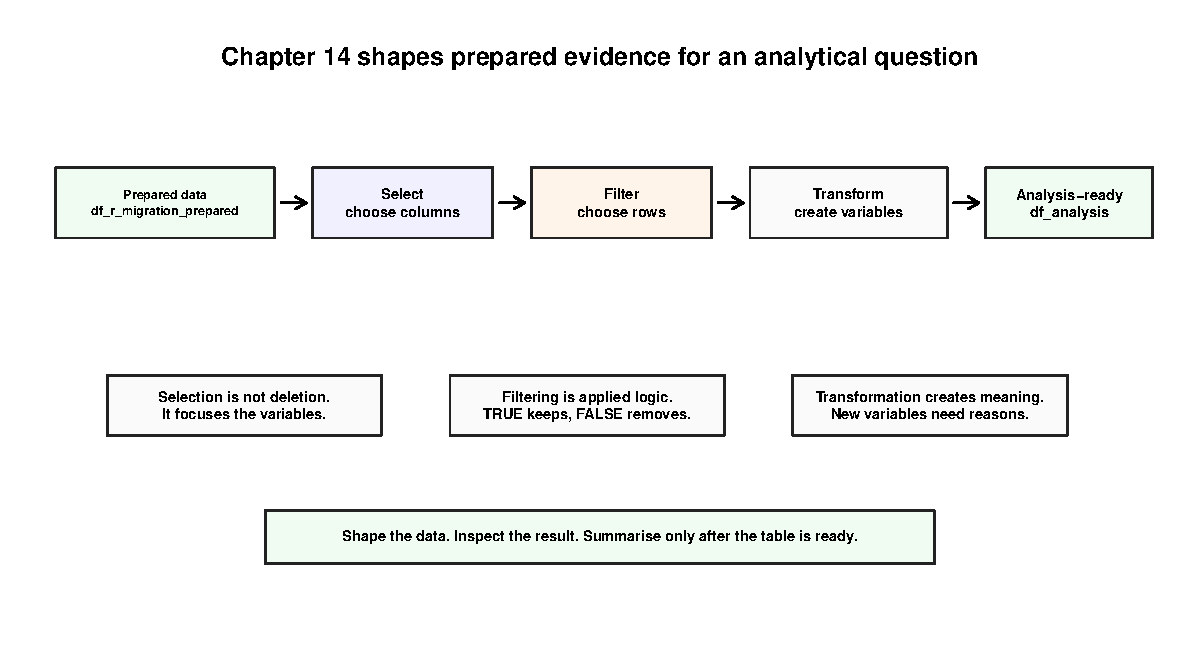
\includegraphics[width=0.9\linewidth,height=\textheight,keepaspectratio]{chapters/14-selecting-filtering-and-transforming-data_files/figure-pdf/fig-prepared-to-analysis-ready-1.pdf}

}

\caption{\label{fig-prepared-to-analysis-ready}From Prepared Data to
Analysis-Ready Data}

\end{figure}%

As shown in Figure~\ref{fig-prepared-to-analysis-ready}, Chapter 14 has
a narrower job than Chapter 13 and Chapter 15. It does not clean the raw
evidence, and it does not yet reduce many rows into summaries. It shapes
prepared evidence into a focused object that can support summary work
later.

That focus protects the workflow.

\section{Selection, Filtering, and Transformation Are Different
Moves}\label{selection-filtering-and-transformation-are-different-moves}

Data shaping becomes easier when Leo can name the move he is making.
Table~\ref{tbl-data-shaping-moves} summarises the core moves in this
chapter.

\begin{longtable}[]{@{}
  >{\raggedright\arraybackslash}p{(\linewidth - 6\tabcolsep) * \real{0.2500}}
  >{\raggedright\arraybackslash}p{(\linewidth - 6\tabcolsep) * \real{0.2500}}
  >{\raggedright\arraybackslash}p{(\linewidth - 6\tabcolsep) * \real{0.2500}}
  >{\raggedright\arraybackslash}p{(\linewidth - 6\tabcolsep) * \real{0.2500}}@{}}
\caption{Core data-shaping moves in Chapter
14}\label{tbl-data-shaping-moves}\tabularnewline
\toprule\noalign{}
\begin{minipage}[b]{\linewidth}\raggedright
Move
\end{minipage} & \begin{minipage}[b]{\linewidth}\raggedright
Main question
\end{minipage} & \begin{minipage}[b]{\linewidth}\raggedright
Base R pattern
\end{minipage} & \begin{minipage}[b]{\linewidth}\raggedright
Tidyverse pattern
\end{minipage} \\
\midrule\noalign{}
\endfirsthead
\toprule\noalign{}
\begin{minipage}[b]{\linewidth}\raggedright
Move
\end{minipage} & \begin{minipage}[b]{\linewidth}\raggedright
Main question
\end{minipage} & \begin{minipage}[b]{\linewidth}\raggedright
Base R pattern
\end{minipage} & \begin{minipage}[b]{\linewidth}\raggedright
Tidyverse pattern
\end{minipage} \\
\midrule\noalign{}
\endhead
\bottomrule\noalign{}
\endlastfoot
Select & Which variables matter? & \texttt{df{[}c("x",\ "y"){]}} &
\texttt{select(x,\ y)} \\
Filter & Which rows matter? &
\texttt{df{[}df\$x\ \textgreater{}\ 5,\ {]}} &
\texttt{filter(x\ \textgreater{}\ 5)} \\
Rename & Would clearer names help? &
\texttt{names(df){[}...{]}\ \textless{}-\ ...} &
\texttt{rename(new\ =\ old)} \\
Arrange & What order helps inspection? &
\texttt{df{[}order(df\$x),\ {]}} & \texttt{arrange(x)} \\
Transform & What new variable is needed? &
\texttt{df\$new\ \textless{}-\ ...} & \texttt{mutate(new\ =\ ...)} \\
\end{longtable}

The table is not a memorisation list. It is a map.

Selection is about variables. Filtering is about observations.
Transformation is about meaning. Arrangement is about inspection.
Renaming is about clarity.

The same prepared data can be shaped in many ways depending on the
question. That is why Leo should not shape data blindly. He should first
ask what question the table needs to help answer.

\begin{tcolorbox}[enhanced jigsaw, arc=.35mm, bottomrule=.15mm, breakable, colback=white, colframe=quarto-callout-tip-color-frame, left=2mm, leftrule=.75mm, opacityback=0, rightrule=.15mm, toprule=.15mm]
\begin{minipage}[t]{5.5mm}
\textcolor{quarto-callout-tip-color}{\faLightbulb}
\end{minipage}%
\begin{minipage}[t]{\textwidth - 5.5mm}

\vspace{-3mm}\textbf{Core Mental Model}\vspace{3mm}

Selection asks which columns matter. Filtering asks which rows matter.
Transformation asks what new analytical meaning should be created.

\end{minipage}%
\end{tcolorbox}

\section{Base R and Tidyverse: Two Ways to Express the Same
Move}\label{base-r-and-tidyverse-two-ways-to-express-the-same-move}

Chapter 11 gave Leo a practical rule:

\begin{quote}
Base R teaches the structure of the language. Tidyverse teaches workflow
fluency. Serious R users eventually understand both.
\end{quote}

That rule matters here.

Base R often shows what is happening underneath. Tidyverse code often
reads like a workflow. Leo does not need to choose a camp. He needs to
understand the move.

In this chapter, some examples show both forms. The purpose is not to
double the burden. The purpose is to help Leo recognise that the same
data-shaping idea can be expressed in more than one R grammar.

\section{Selecting Variables: Which Columns
Matter?}\label{selecting-variables-which-columns-matter}

A prepared dataset may contain more variables than Leo needs for a
specific question. Selection lets him choose the columns that matter for
the current task.

Suppose Leo wants a focused learner-performance table. He may begin with
these variables:

\begin{Shaded}
\begin{Highlighting}[]
\NormalTok{learner\_id}
\NormalTok{country}
\NormalTok{background}
\NormalTok{r\_experience\_level}
\NormalTok{study\_hours}
\NormalTok{lessons\_completed}
\NormalTok{pre\_assessment\_score}
\NormalTok{project\_score}
\NormalTok{completion\_status}
\NormalTok{first\_script\_completed}
\NormalTok{used\_quarto}
\NormalTok{used\_git}
\end{Highlighting}
\end{Shaded}

In Base R, he can select columns by name:

\begin{Shaded}
\begin{Highlighting}[]
\NormalTok{performance\_columns }\OtherTok{\textless{}{-}} \FunctionTok{c}\NormalTok{(}
  \StringTok{"learner\_id"}\NormalTok{,}
  \StringTok{"country"}\NormalTok{,}
  \StringTok{"background"}\NormalTok{,}
  \StringTok{"r\_experience\_level"}\NormalTok{,}
  \StringTok{"study\_hours"}\NormalTok{,}
  \StringTok{"lessons\_completed"}\NormalTok{,}
  \StringTok{"pre\_assessment\_score"}\NormalTok{,}
  \StringTok{"project\_score"}\NormalTok{,}
  \StringTok{"completion\_status"}\NormalTok{,}
  \StringTok{"first\_script\_completed"}\NormalTok{,}
  \StringTok{"used\_quarto"}\NormalTok{,}
  \StringTok{"used\_git"}
\NormalTok{)}

\NormalTok{df\_selected }\OtherTok{\textless{}{-}}\NormalTok{ df\_r\_migration\_prepared[performance\_columns]}
\end{Highlighting}
\end{Shaded}

In tidyverse style, he can express the same choice with
\texttt{dplyr::select()}:

\begin{Shaded}
\begin{Highlighting}[]
\NormalTok{df\_selected }\OtherTok{\textless{}{-}}\NormalTok{ df\_r\_migration\_prepared }\SpecialCharTok{|\textgreater{}}
\NormalTok{  dplyr}\SpecialCharTok{::}\FunctionTok{select}\NormalTok{(}
\NormalTok{    learner\_id,}
\NormalTok{    country,}
\NormalTok{    background,}
\NormalTok{    r\_experience\_level,}
\NormalTok{    study\_hours,}
\NormalTok{    lessons\_completed,}
\NormalTok{    pre\_assessment\_score,}
\NormalTok{    project\_score,}
\NormalTok{    completion\_status,}
\NormalTok{    first\_script\_completed,}
\NormalTok{    used\_quarto,}
\NormalTok{    used\_git}
\NormalTok{  )}
\end{Highlighting}
\end{Shaded}

Both examples answer the same question:

\begin{quote}
Which variables does this analysis need right now?
\end{quote}

Selection is not deletion. The original prepared object remains
available. Leo is creating a focused view for a purpose.

After selecting, he should inspect:

\begin{Shaded}
\begin{Highlighting}[]
\FunctionTok{names}\NormalTok{(df\_selected)}
\FunctionTok{dim}\NormalTok{(df\_selected)}
\FunctionTok{head}\NormalTok{(df\_selected)}
\end{Highlighting}
\end{Shaded}

A shaping move without inspection is only a guess.

\section{Renaming for Clarity}\label{renaming-for-clarity}

Renaming is useful when a name is technically valid but could be clearer
in a specific analysis object.

For example, \texttt{project\_score} is already clear. Leo does not need
to rename it. But in a focused analysis table, he might decide that
\texttt{pre\_assessment\_score} is too long for repeated work and prefer
\texttt{pre\_score}.

In Base R:

\begin{Shaded}
\begin{Highlighting}[]
\FunctionTok{names}\NormalTok{(df\_selected)[}\FunctionTok{names}\NormalTok{(df\_selected) }\SpecialCharTok{==} \StringTok{"pre\_assessment\_score"}\NormalTok{] }\OtherTok{\textless{}{-}} \StringTok{"pre\_score"}
\end{Highlighting}
\end{Shaded}

In tidyverse style:

\begin{Shaded}
\begin{Highlighting}[]
\NormalTok{df\_selected }\OtherTok{\textless{}{-}}\NormalTok{ df\_selected }\SpecialCharTok{|\textgreater{}}
\NormalTok{  dplyr}\SpecialCharTok{::}\FunctionTok{rename}\NormalTok{(}\AttributeTok{pre\_score =}\NormalTok{ pre\_assessment\_score)}
\end{Highlighting}
\end{Shaded}

Renaming should be done sparingly. A clearer name helps the reader. Too
many unnecessary renamings make the evidence harder to trace.

A useful rule is:

\begin{quote}
Rename only when clarity improves enough to justify the extra
translation.
\end{quote}

\section{Filtering Observations: Which Rows Answer the
Question?}\label{filtering-observations-which-rows-answer-the-question}

Selection chooses columns. Filtering chooses rows.

Filtering is where Part 2 logic becomes practical. A filter is not
magic. It is a logical judgment applied to every row. If the condition
returns \texttt{TRUE} for a row, the row remains. If it returns
\texttt{FALSE}, the row is removed from the result.

Suppose Leo wants records with more than five study hours.

In Base R:

\begin{Shaded}
\begin{Highlighting}[]
\NormalTok{df\_more\_study }\OtherTok{\textless{}{-}}\NormalTok{ df\_r\_migration\_prepared[}
  \SpecialCharTok{!}\FunctionTok{is.na}\NormalTok{(df\_r\_migration\_prepared}\SpecialCharTok{$}\NormalTok{study\_hours) }\SpecialCharTok{\&}
\NormalTok{    df\_r\_migration\_prepared}\SpecialCharTok{$}\NormalTok{study\_hours }\SpecialCharTok{\textgreater{}} \DecValTok{5}\NormalTok{,}
\NormalTok{]}
\end{Highlighting}
\end{Shaded}

In tidyverse style:

\begin{Shaded}
\begin{Highlighting}[]
\NormalTok{df\_more\_study }\OtherTok{\textless{}{-}}\NormalTok{ df\_r\_migration\_prepared }\SpecialCharTok{|\textgreater{}}
\NormalTok{  dplyr}\SpecialCharTok{::}\FunctionTok{filter}\NormalTok{(}
    \SpecialCharTok{!}\FunctionTok{is.na}\NormalTok{(study\_hours),}
\NormalTok{    study\_hours }\SpecialCharTok{\textgreater{}} \DecValTok{5}
\NormalTok{  )}
\end{Highlighting}
\end{Shaded}

Both versions rely on the same logical idea:

\begin{Shaded}
\begin{Highlighting}[]
\NormalTok{study\_hours }\SpecialCharTok{\textgreater{}} \DecValTok{5}
\end{Highlighting}
\end{Shaded}

That condition produces a row-by-row judgment. Chapter 7 prepared Leo
for this. Filtering is logical judgment turned into row selection.

\section{Filtering with Missing
Values}\label{filtering-with-missing-values}

Filtering becomes more delicate when a variable may contain missing
values.

Suppose Leo wants records where \texttt{project\_score} is at least 80.
If some project scores are missing, he should be explicit about what he
wants.

In Base R:

\begin{Shaded}
\begin{Highlighting}[]
\NormalTok{df\_high\_scores }\OtherTok{\textless{}{-}}\NormalTok{ df\_r\_migration\_prepared[}
  \SpecialCharTok{!}\FunctionTok{is.na}\NormalTok{(df\_r\_migration\_prepared}\SpecialCharTok{$}\NormalTok{project\_score) }\SpecialCharTok{\&}
\NormalTok{    df\_r\_migration\_prepared}\SpecialCharTok{$}\NormalTok{project\_score }\SpecialCharTok{\textgreater{}=} \DecValTok{80}\NormalTok{,}
\NormalTok{]}
\end{Highlighting}
\end{Shaded}

In tidyverse style:

\begin{Shaded}
\begin{Highlighting}[]
\NormalTok{df\_high\_scores }\OtherTok{\textless{}{-}}\NormalTok{ df\_r\_migration\_prepared }\SpecialCharTok{|\textgreater{}}
\NormalTok{  dplyr}\SpecialCharTok{::}\FunctionTok{filter}\NormalTok{(}
    \SpecialCharTok{!}\FunctionTok{is.na}\NormalTok{(project\_score),}
\NormalTok{    project\_score }\SpecialCharTok{\textgreater{}=} \DecValTok{80}
\NormalTok{  )}
\end{Highlighting}
\end{Shaded}

The \texttt{!is.na(project\_score)} condition says: keep only rows where
the project score is known.

This is not just technical tidiness. It is analytical honesty. Leo
should know whether a row is excluded because it failed a condition or
because the value needed for judgment was missing.

\begin{tcolorbox}[enhanced jigsaw, arc=.35mm, bottomrule=.15mm, breakable, colback=white, colframe=quarto-callout-important-color-frame, left=2mm, leftrule=.75mm, opacityback=0, rightrule=.15mm, toprule=.15mm]
\begin{minipage}[t]{5.5mm}
\textcolor{quarto-callout-important-color}{\faExclamation}
\end{minipage}%
\begin{minipage}[t]{\textwidth - 5.5mm}

\vspace{-3mm}\textbf{Reliable Analysis Rule}\vspace{3mm}

A filter is a judgment. If a value is missing, the judgment may be
uncertain. Use \texttt{is.na()} or \texttt{!is.na()} deliberately rather
than pretending missingness has no effect.

\end{minipage}%
\end{tcolorbox}

\section{Combining Conditions}\label{combining-conditions}

Real questions often need more than one condition.

Suppose Leo wants learners who studied more than five hours and scored
at least 80 on the project.

In Base R:

\begin{Shaded}
\begin{Highlighting}[]
\NormalTok{df\_focused }\OtherTok{\textless{}{-}}\NormalTok{ df\_r\_migration\_prepared[}
  \SpecialCharTok{!}\FunctionTok{is.na}\NormalTok{(df\_r\_migration\_prepared}\SpecialCharTok{$}\NormalTok{study\_hours) }\SpecialCharTok{\&}
    \SpecialCharTok{!}\FunctionTok{is.na}\NormalTok{(df\_r\_migration\_prepared}\SpecialCharTok{$}\NormalTok{project\_score) }\SpecialCharTok{\&}
\NormalTok{    df\_r\_migration\_prepared}\SpecialCharTok{$}\NormalTok{study\_hours }\SpecialCharTok{\textgreater{}} \DecValTok{5} \SpecialCharTok{\&}
\NormalTok{    df\_r\_migration\_prepared}\SpecialCharTok{$}\NormalTok{project\_score }\SpecialCharTok{\textgreater{}=} \DecValTok{80}\NormalTok{,}
\NormalTok{]}
\end{Highlighting}
\end{Shaded}

In tidyverse style:

\begin{Shaded}
\begin{Highlighting}[]
\NormalTok{df\_focused }\OtherTok{\textless{}{-}}\NormalTok{ df\_r\_migration\_prepared }\SpecialCharTok{|\textgreater{}}
\NormalTok{  dplyr}\SpecialCharTok{::}\FunctionTok{filter}\NormalTok{(}
    \SpecialCharTok{!}\FunctionTok{is.na}\NormalTok{(study\_hours),}
    \SpecialCharTok{!}\FunctionTok{is.na}\NormalTok{(project\_score),}
\NormalTok{    study\_hours }\SpecialCharTok{\textgreater{}} \DecValTok{5}\NormalTok{,}
\NormalTok{    project\_score }\SpecialCharTok{\textgreater{}=} \DecValTok{80}
\NormalTok{  )}
\end{Highlighting}
\end{Shaded}

The \texttt{\&} operator is doing vectorised logic. It checks conditions
row by row.

This matters. Leo should use \texttt{\&} for row-wise filtering. He
should not use \texttt{\&\&} here. The double form, \texttt{\&\&}, is
mainly for single control-flow decisions, not filtering many rows in a
data frame.

\begin{tcolorbox}[enhanced jigsaw, arc=.35mm, bottomrule=.15mm, breakable, colback=white, colframe=quarto-callout-warning-color-frame, left=2mm, leftrule=.75mm, opacityback=0, rightrule=.15mm, toprule=.15mm]
\begin{minipage}[t]{5.5mm}
\textcolor{quarto-callout-warning-color}{\faExclamationTriangle}
\end{minipage}%
\begin{minipage}[t]{\textwidth - 5.5mm}

\vspace{-3mm}\textbf{Common Beginner Trap}\vspace{3mm}

For data-frame filtering, use \texttt{\&} and \texttt{\textbar{}} for
row-by-row logic. Do not use \texttt{\&\&} and
\texttt{\textbar{}\textbar{}} to filter many rows.

\end{minipage}%
\end{tcolorbox}

\section{Filtering with a Set of
Values}\label{filtering-with-a-set-of-values}

Sometimes Leo does not want one category. He wants any value from a
small set.

For example, he may want records from selected countries:

\begin{Shaded}
\begin{Highlighting}[]
\NormalTok{target\_countries }\OtherTok{\textless{}{-}} \FunctionTok{c}\NormalTok{(}\StringTok{"nigeria"}\NormalTok{, }\StringTok{"kenya"}\NormalTok{, }\StringTok{"south africa"}\NormalTok{)}
\end{Highlighting}
\end{Shaded}

In Base R:

\begin{Shaded}
\begin{Highlighting}[]
\NormalTok{df\_countries }\OtherTok{\textless{}{-}}\NormalTok{ df\_r\_migration\_prepared[}
\NormalTok{  df\_r\_migration\_prepared}\SpecialCharTok{$}\NormalTok{country }\SpecialCharTok{\%in\%}\NormalTok{ target\_countries,}
\NormalTok{]}
\end{Highlighting}
\end{Shaded}

In tidyverse style:

\begin{Shaded}
\begin{Highlighting}[]
\NormalTok{df\_countries }\OtherTok{\textless{}{-}}\NormalTok{ df\_r\_migration\_prepared }\SpecialCharTok{|\textgreater{}}
\NormalTok{  dplyr}\SpecialCharTok{::}\FunctionTok{filter}\NormalTok{(country }\SpecialCharTok{\%in\%}\NormalTok{ target\_countries)}
\end{Highlighting}
\end{Shaded}

The \texttt{\%in\%} operator asks:

\begin{quote}
Is this value one of the values in the set?
\end{quote}

It is often clearer than writing several \texttt{\textbar{}} conditions.

\section{Arranging Rows for
Inspection}\label{arranging-rows-for-inspection}

Arranging rows changes order. It does not remove observations and it
does not create new variables.

Leo may arrange project scores from highest to lowest so strong records
are easier to inspect.

In Base R:

\begin{Shaded}
\begin{Highlighting}[]
\NormalTok{df\_arranged }\OtherTok{\textless{}{-}}\NormalTok{ df\_r\_migration\_prepared[}
  \FunctionTok{order}\NormalTok{(df\_r\_migration\_prepared}\SpecialCharTok{$}\NormalTok{project\_score, }\AttributeTok{decreasing =} \ConstantTok{TRUE}\NormalTok{),}
\NormalTok{]}
\end{Highlighting}
\end{Shaded}

In tidyverse style:

\begin{Shaded}
\begin{Highlighting}[]
\NormalTok{df\_arranged }\OtherTok{\textless{}{-}}\NormalTok{ df\_r\_migration\_prepared }\SpecialCharTok{|\textgreater{}}
\NormalTok{  dplyr}\SpecialCharTok{::}\FunctionTok{arrange}\NormalTok{(dplyr}\SpecialCharTok{::}\FunctionTok{desc}\NormalTok{(project\_score))}
\end{Highlighting}
\end{Shaded}

Arrangement is useful for inspection. It is not a summary. If Leo wants
the average score by country, that is Chapter 15.

\section{Transforming Variables: Creating Clearer
Evidence}\label{transforming-variables-creating-clearer-evidence}

Transformation creates or modifies variables so that the data can answer
a question more clearly.

This is different from cleaning.

Cleaning standardises evidence so it can be trusted. Transformation
creates analytical meaning from prepared evidence.

A simple transformation is a logical flag:

\begin{Shaded}
\begin{Highlighting}[]
\NormalTok{df\_r\_migration\_prepared}\SpecialCharTok{$}\NormalTok{high\_project\_score }\OtherTok{\textless{}{-}}
\NormalTok{  df\_r\_migration\_prepared}\SpecialCharTok{$}\NormalTok{project\_score }\SpecialCharTok{\textgreater{}=} \DecValTok{80}
\end{Highlighting}
\end{Shaded}

The tidyverse version is:

\begin{Shaded}
\begin{Highlighting}[]
\NormalTok{df\_r\_migration\_prepared }\OtherTok{\textless{}{-}}\NormalTok{ df\_r\_migration\_prepared }\SpecialCharTok{|\textgreater{}}
\NormalTok{  dplyr}\SpecialCharTok{::}\FunctionTok{mutate}\NormalTok{(}
    \AttributeTok{high\_project\_score =}\NormalTok{ project\_score }\SpecialCharTok{\textgreater{}=} \DecValTok{80}
\NormalTok{  )}
\end{Highlighting}
\end{Shaded}

This new variable asks a clear question:

\begin{quote}
Did this record reach a project score of 80 or above?
\end{quote}

The answer is a logical value: \texttt{TRUE}, \texttt{FALSE}, or
possibly \texttt{NA} if the score is missing.

Leo has already met this idea in Chapter 7. Logical values are not
decorations. They can guide later selection and summary.

\section{Creating a Score Gap}\label{creating-a-score-gap}

Leo may want to compare project performance with the earlier
pre-assessment score.

A simple derived variable is:

\begin{Shaded}
\begin{Highlighting}[]
\NormalTok{score\_gap = project\_score {-} pre\_assessment\_score}
\end{Highlighting}
\end{Shaded}

In Base R:

\begin{Shaded}
\begin{Highlighting}[]
\NormalTok{df\_r\_migration\_prepared}\SpecialCharTok{$}\NormalTok{score\_gap }\OtherTok{\textless{}{-}}
\NormalTok{  df\_r\_migration\_prepared}\SpecialCharTok{$}\NormalTok{project\_score }\SpecialCharTok{{-}}
\NormalTok{  df\_r\_migration\_prepared}\SpecialCharTok{$}\NormalTok{pre\_assessment\_score}
\end{Highlighting}
\end{Shaded}

In tidyverse style:

\begin{Shaded}
\begin{Highlighting}[]
\NormalTok{df\_r\_migration\_prepared }\OtherTok{\textless{}{-}}\NormalTok{ df\_r\_migration\_prepared }\SpecialCharTok{|\textgreater{}}
\NormalTok{  dplyr}\SpecialCharTok{::}\FunctionTok{mutate}\NormalTok{(}
    \AttributeTok{score\_gap =}\NormalTok{ project\_score }\SpecialCharTok{{-}}\NormalTok{ pre\_assessment\_score}
\NormalTok{  )}
\end{Highlighting}
\end{Shaded}

This transformation has a reason. It gives Leo a way to ask whether
learners improved from pre-assessment to project performance.

He should inspect it:

\begin{Shaded}
\begin{Highlighting}[]
\FunctionTok{summary}\NormalTok{(df\_r\_migration\_prepared}\SpecialCharTok{$}\NormalTok{score\_gap)}
\end{Highlighting}
\end{Shaded}

If the summary shows strange values, he should not ignore them. A new
variable deserves the same inspection as an imported one.

\section{Creating Study Bands}\label{creating-study-bands}

A continuous numeric variable can sometimes be turned into a broad
category for easier interpretation.

For example, Leo may want a simple study-time band.

In Base R:

\begin{Shaded}
\begin{Highlighting}[]
\NormalTok{df\_r\_migration\_prepared}\SpecialCharTok{$}\NormalTok{study\_band }\OtherTok{\textless{}{-}} \FunctionTok{ifelse}\NormalTok{(}
  \FunctionTok{is.na}\NormalTok{(df\_r\_migration\_prepared}\SpecialCharTok{$}\NormalTok{study\_hours),}
  \ConstantTok{NA}\NormalTok{,}
  \FunctionTok{ifelse}\NormalTok{(}
\NormalTok{    df\_r\_migration\_prepared}\SpecialCharTok{$}\NormalTok{study\_hours }\SpecialCharTok{\textgreater{}=} \DecValTok{7}\NormalTok{,}
    \StringTok{"higher study time"}\NormalTok{,}
    \StringTok{"lower study time"}
\NormalTok{  )}
\NormalTok{)}
\end{Highlighting}
\end{Shaded}

In tidyverse style:

\begin{Shaded}
\begin{Highlighting}[]
\NormalTok{df\_r\_migration\_prepared }\OtherTok{\textless{}{-}}\NormalTok{ df\_r\_migration\_prepared }\SpecialCharTok{|\textgreater{}}
\NormalTok{  dplyr}\SpecialCharTok{::}\FunctionTok{mutate}\NormalTok{(}
    \AttributeTok{study\_band =}\NormalTok{ dplyr}\SpecialCharTok{::}\FunctionTok{case\_when}\NormalTok{(}
      \FunctionTok{is.na}\NormalTok{(study\_hours) }\SpecialCharTok{\textasciitilde{}} \ConstantTok{NA\_character\_}\NormalTok{,}
\NormalTok{      study\_hours }\SpecialCharTok{\textgreater{}=} \DecValTok{7} \SpecialCharTok{\textasciitilde{}} \StringTok{"higher study time"}\NormalTok{,}
\NormalTok{      study\_hours }\SpecialCharTok{\textless{}} \DecValTok{7} \SpecialCharTok{\textasciitilde{}} \StringTok{"lower study time"}
\NormalTok{    )}
\NormalTok{  )}
\end{Highlighting}
\end{Shaded}

This example introduces a useful pattern. \texttt{ifelse()} is a Base R
function for conditional values. \texttt{case\_when()} is a tidyverse
function for writing several conditional rules more readably.

Do not make categories just because categories are convenient. A
category should help the analysis communicate a meaningful distinction.

\section{Creating Tool Readiness}\label{creating-tool-readiness}

The prepared dataset includes tool-use fields:

\begin{Shaded}
\begin{Highlighting}[]
\NormalTok{used\_rstudio}
\NormalTok{used\_quarto}
\NormalTok{used\_git}
\NormalTok{used\_renv}
\end{Highlighting}
\end{Shaded}

After Chapter 13, these fields should be prepared as logical values. Leo
can use them to create a simple readiness indicator.

For example:

\begin{Shaded}
\begin{Highlighting}[]
\NormalTok{df\_r\_migration\_prepared }\OtherTok{\textless{}{-}}\NormalTok{ df\_r\_migration\_prepared }\SpecialCharTok{|\textgreater{}}
\NormalTok{  dplyr}\SpecialCharTok{::}\FunctionTok{mutate}\NormalTok{(}
    \AttributeTok{tool\_readiness =}\NormalTok{ dplyr}\SpecialCharTok{::}\FunctionTok{case\_when}\NormalTok{(}
\NormalTok{      dplyr}\SpecialCharTok{::}\FunctionTok{if\_any}\NormalTok{(}
        \FunctionTok{c}\NormalTok{(used\_rstudio, used\_quarto, used\_git, used\_renv),}
\NormalTok{        is.na}
\NormalTok{      ) }\SpecialCharTok{\textasciitilde{}} \StringTok{"unknown tool readiness"}\NormalTok{,}
\NormalTok{      used\_rstudio }\SpecialCharTok{\&}\NormalTok{ used\_quarto }\SpecialCharTok{\&}\NormalTok{ used\_git }\SpecialCharTok{\&}\NormalTok{ used\_renv }\SpecialCharTok{\textasciitilde{}} \StringTok{"full tool readiness"}\NormalTok{,}
\NormalTok{      used\_rstudio }\SpecialCharTok{\&}\NormalTok{ used\_quarto }\SpecialCharTok{\textasciitilde{}} \StringTok{"reporting readiness"}\NormalTok{,}
\NormalTok{      used\_rstudio }\SpecialCharTok{\textasciitilde{}} \StringTok{"basic RStudio readiness"}\NormalTok{,}
      \ConstantTok{TRUE} \SpecialCharTok{\textasciitilde{}} \StringTok{"needs tool support"}
\NormalTok{    )}
\NormalTok{  )}
\end{Highlighting}
\end{Shaded}

This is a transformation because Leo is creating a new analytical label
from existing variables.

It is not a cleaning step. The logical fields should already have been
prepared in Chapter 13. Chapter 14 uses them to express a new idea.

If this rule appears repeatedly in later work, Chapter 9's lesson
returns: repeated logic can become a small named helper function. That
does not need to happen here, but Leo should recognise the pattern.

\section{Transformation Is Not
Cleaning}\label{transformation-is-not-cleaning}

It is easy to confuse cleaning and transformation because both can
change columns.

The difference is purpose.

Cleaning asks:

\begin{quote}
Is this evidence consistent enough to work with?
\end{quote}

Transformation asks:

\begin{quote}
What new analytical meaning should this prepared evidence express?
\end{quote}

For example, standardising \texttt{country} from \texttt{"\ Nigeria\ "}
and \texttt{"NIGERIA"} into \texttt{"nigeria"} is cleaning. Creating
\texttt{high\_project\_score} from
\texttt{project\_score\ \textgreater{}=\ 80} is transformation. Turning
\texttt{study\_hours} into \texttt{study\_band} is transformation.
Creating \texttt{score\_gap} from
\texttt{project\_score\ -\ pre\_assessment\_score} is transformation.

\begin{tcolorbox}[enhanced jigsaw, arc=.35mm, bottomrule=.15mm, breakable, colback=white, colframe=quarto-callout-note-color-frame, left=2mm, leftrule=.75mm, opacityback=0, rightrule=.15mm, toprule=.15mm]
\begin{minipage}[t]{5.5mm}
\textcolor{quarto-callout-note-color}{\faInfo}
\end{minipage}%
\begin{minipage}[t]{\textwidth - 5.5mm}

\vspace{-3mm}\textbf{Boundary Note}\vspace{3mm}

Chapter 13 made the evidence more consistent. Chapter 14 shapes that
evidence for a question. Chapter 15 will summarise and group the shaped
data.

\end{minipage}%
\end{tcolorbox}

\section{Building a Small Analysis-Ready
Dataset}\label{building-a-small-analysis-ready-dataset}

Now Leo can combine the moves.

He begins with the prepared object:

\begin{Shaded}
\begin{Highlighting}[]
\NormalTok{df\_r\_migration\_prepared}
\end{Highlighting}
\end{Shaded}

Then he creates a focused analysis object:

\begin{Shaded}
\begin{Highlighting}[]
\NormalTok{df\_analysis}
\end{Highlighting}
\end{Shaded}

Here is one tidyverse workflow:

\begin{Shaded}
\begin{Highlighting}[]
\NormalTok{df\_analysis }\OtherTok{\textless{}{-}}\NormalTok{ df\_r\_migration\_prepared }\SpecialCharTok{|\textgreater{}}
\NormalTok{  dplyr}\SpecialCharTok{::}\FunctionTok{select}\NormalTok{(}
\NormalTok{    learner\_id,}
\NormalTok{    country,}
\NormalTok{    region,}
\NormalTok{    job\_role,}
\NormalTok{    industry,}
\NormalTok{    background,}
\NormalTok{    r\_experience\_level,}
\NormalTok{    week,}
\NormalTok{    study\_hours,}
\NormalTok{    lessons\_completed,}
\NormalTok{    confidence\_score,}
\NormalTok{    pre\_assessment\_score,}
\NormalTok{    project\_score,}
\NormalTok{    completion\_status,}
\NormalTok{    first\_script\_completed,}
\NormalTok{    used\_rstudio,}
\NormalTok{    used\_quarto,}
\NormalTok{    used\_git,}
\NormalTok{    used\_renv,}
\NormalTok{    preferred\_learning\_mode,}
\NormalTok{    monthly\_income\_band,}
\NormalTok{    manager\_support,}
\NormalTok{    payment\_probability\_score}
\NormalTok{  ) }\SpecialCharTok{|\textgreater{}}
\NormalTok{  dplyr}\SpecialCharTok{::}\FunctionTok{filter}\NormalTok{(}
    \SpecialCharTok{!}\FunctionTok{is.na}\NormalTok{(study\_hours),}
    \SpecialCharTok{!}\FunctionTok{is.na}\NormalTok{(pre\_assessment\_score),}
    \SpecialCharTok{!}\FunctionTok{is.na}\NormalTok{(project\_score),}
\NormalTok{    study\_hours }\SpecialCharTok{\textgreater{}=} \DecValTok{0}\NormalTok{,}
\NormalTok{    project\_score }\SpecialCharTok{\textgreater{}=} \DecValTok{0}\NormalTok{,}
\NormalTok{    project\_score }\SpecialCharTok{\textless{}=} \DecValTok{100}
\NormalTok{  ) }\SpecialCharTok{|\textgreater{}}
\NormalTok{  dplyr}\SpecialCharTok{::}\FunctionTok{mutate}\NormalTok{(}
    \AttributeTok{high\_project\_score =}\NormalTok{ project\_score }\SpecialCharTok{\textgreater{}=} \DecValTok{80}\NormalTok{,}
    \AttributeTok{score\_gap =}\NormalTok{ project\_score }\SpecialCharTok{{-}}\NormalTok{ pre\_assessment\_score,}
    \AttributeTok{study\_band =}\NormalTok{ dplyr}\SpecialCharTok{::}\FunctionTok{case\_when}\NormalTok{(}
      \FunctionTok{is.na}\NormalTok{(study\_hours) }\SpecialCharTok{\textasciitilde{}} \ConstantTok{NA\_character\_}\NormalTok{,}
\NormalTok{      study\_hours }\SpecialCharTok{\textless{}} \DecValTok{4} \SpecialCharTok{\textasciitilde{}} \StringTok{"Low study time"}\NormalTok{,}
\NormalTok{      study\_hours }\SpecialCharTok{\textless{}} \DecValTok{8} \SpecialCharTok{\textasciitilde{}} \StringTok{"Moderate study time"}\NormalTok{,}
      \ConstantTok{TRUE} \SpecialCharTok{\textasciitilde{}} \StringTok{"High study time"}
\NormalTok{    )}
\NormalTok{  )}
\end{Highlighting}
\end{Shaded}

This code has structure. Chapter 6 helps Leo read it.

The pipe sends the result of one step into the next. \texttt{select()}
narrows the variables to the analysis-ready fields needed for Chapters
15 to 18. \texttt{filter()} keeps records with known study hours and
project scores and removes values that would distort early
visualisation. \texttt{mutate()} creates variables for later summary and
plotting work.

Here is a Base R version of the same general movement:

\begin{Shaded}
\begin{Highlighting}[]
\NormalTok{analysis\_columns }\OtherTok{\textless{}{-}} \FunctionTok{c}\NormalTok{(}
  \StringTok{"learner\_id"}\NormalTok{,}
  \StringTok{"country"}\NormalTok{,}
  \StringTok{"region"}\NormalTok{,}
  \StringTok{"job\_role"}\NormalTok{,}
  \StringTok{"industry"}\NormalTok{,}
  \StringTok{"background"}\NormalTok{,}
  \StringTok{"r\_experience\_level"}\NormalTok{,}
  \StringTok{"week"}\NormalTok{,}
  \StringTok{"study\_hours"}\NormalTok{,}
  \StringTok{"lessons\_completed"}\NormalTok{,}
  \StringTok{"confidence\_score"}\NormalTok{,}
  \StringTok{"pre\_assessment\_score"}\NormalTok{,}
  \StringTok{"project\_score"}\NormalTok{,}
  \StringTok{"completion\_status"}\NormalTok{,}
  \StringTok{"first\_script\_completed"}\NormalTok{,}
  \StringTok{"used\_rstudio"}\NormalTok{,}
  \StringTok{"used\_quarto"}\NormalTok{,}
  \StringTok{"used\_git"}\NormalTok{,}
  \StringTok{"used\_renv"}\NormalTok{,}
  \StringTok{"preferred\_learning\_mode"}\NormalTok{,}
  \StringTok{"monthly\_income\_band"}\NormalTok{,}
  \StringTok{"manager\_support"}\NormalTok{,}
  \StringTok{"payment\_probability\_score"}
\NormalTok{)}

\NormalTok{df\_analysis\_base }\OtherTok{\textless{}{-}}\NormalTok{ df\_r\_migration\_prepared[analysis\_columns]}

\NormalTok{df\_analysis\_base }\OtherTok{\textless{}{-}}\NormalTok{ df\_analysis\_base[}
  \SpecialCharTok{!}\FunctionTok{is.na}\NormalTok{(df\_analysis\_base}\SpecialCharTok{$}\NormalTok{study\_hours) }\SpecialCharTok{\&}
    \SpecialCharTok{!}\FunctionTok{is.na}\NormalTok{(df\_analysis\_base}\SpecialCharTok{$}\NormalTok{pre\_assessment\_score) }\SpecialCharTok{\&}
    \SpecialCharTok{!}\FunctionTok{is.na}\NormalTok{(df\_analysis\_base}\SpecialCharTok{$}\NormalTok{project\_score) }\SpecialCharTok{\&}
\NormalTok{    df\_analysis\_base}\SpecialCharTok{$}\NormalTok{study\_hours }\SpecialCharTok{\textgreater{}=} \DecValTok{0} \SpecialCharTok{\&}
\NormalTok{    df\_analysis\_base}\SpecialCharTok{$}\NormalTok{project\_score }\SpecialCharTok{\textgreater{}=} \DecValTok{0} \SpecialCharTok{\&}
\NormalTok{    df\_analysis\_base}\SpecialCharTok{$}\NormalTok{project\_score }\SpecialCharTok{\textless{}=} \DecValTok{100}\NormalTok{,}
\NormalTok{]}

\NormalTok{df\_analysis\_base}\SpecialCharTok{$}\NormalTok{high\_project\_score }\OtherTok{\textless{}{-}}\NormalTok{ df\_analysis\_base}\SpecialCharTok{$}\NormalTok{project\_score }\SpecialCharTok{\textgreater{}=} \DecValTok{80}

\NormalTok{df\_analysis\_base}\SpecialCharTok{$}\NormalTok{score\_gap }\OtherTok{\textless{}{-}}
\NormalTok{  df\_analysis\_base}\SpecialCharTok{$}\NormalTok{project\_score }\SpecialCharTok{{-}}
\NormalTok{  df\_analysis\_base}\SpecialCharTok{$}\NormalTok{pre\_assessment\_score}

\NormalTok{df\_analysis\_base}\SpecialCharTok{$}\NormalTok{study\_band }\OtherTok{\textless{}{-}} \FunctionTok{ifelse}\NormalTok{(}
  \FunctionTok{is.na}\NormalTok{(df\_analysis\_base}\SpecialCharTok{$}\NormalTok{study\_hours),}
  \ConstantTok{NA}\NormalTok{,}
  \FunctionTok{ifelse}\NormalTok{(}
\NormalTok{    df\_analysis\_base}\SpecialCharTok{$}\NormalTok{study\_hours }\SpecialCharTok{\textless{}} \DecValTok{4}\NormalTok{,}
    \StringTok{"Low study time"}\NormalTok{,}
    \FunctionTok{ifelse}\NormalTok{(}
\NormalTok{      df\_analysis\_base}\SpecialCharTok{$}\NormalTok{study\_hours }\SpecialCharTok{\textless{}} \DecValTok{8}\NormalTok{,}
      \StringTok{"Moderate study time"}\NormalTok{,}
      \StringTok{"High study time"}
\NormalTok{    )}
\NormalTok{  )}
\NormalTok{)}
\end{Highlighting}
\end{Shaded}

The tidyverse version reads as one workflow. The Base R version makes
the indexing and assignment explicit. Both are valuable.

The important point is that Leo can explain the movement.

\section{Checking After Every Move}\label{checking-after-every-move}

A shaped dataset must be inspected.

After creating \texttt{df\_analysis}, Leo should ask:

\begin{Shaded}
\begin{Highlighting}[]
\FunctionTok{names}\NormalTok{(df\_analysis)}
\FunctionTok{dim}\NormalTok{(df\_analysis)}
\FunctionTok{str}\NormalTok{(df\_analysis)}
\FunctionTok{head}\NormalTok{(df\_analysis)}
\FunctionTok{summary}\NormalTok{(df\_analysis}\SpecialCharTok{$}\NormalTok{score\_gap)}
\FunctionTok{table}\NormalTok{(df\_analysis}\SpecialCharTok{$}\NormalTok{high\_project\_score, }\AttributeTok{useNA =} \StringTok{"ifany"}\NormalTok{)}
\end{Highlighting}
\end{Shaded}

These checks are not optional decorations. They protect analysis from
silent mistakes.

If \texttt{df\_analysis} has fewer rows than expected, Leo should ask
which filter removed them. If \texttt{score\_gap} contains unexpected
values, he should inspect the source variables. If
\texttt{high\_project\_score} has many missing values, he should check
whether \texttt{project\_score} was missing.

This is Part 2 returning inside Part 3.

Syntax gives the workflow its structure. Logic powers the filters.
Built-in functions perform the checks. Repeated transformation rules can
later become named helper functions.

\section{Common Beginner Mistakes}\label{common-beginner-mistakes-6}

\subsection{Mistake 1: Selecting columns before understanding the
question}\label{mistake-1-selecting-columns-before-understanding-the-question}

Selection should follow purpose. Choosing fewer columns can make a
dataset easier to work with, but only if Leo knows why those columns
matter.

\subsection{Mistake 2: Treating selection as
deletion}\label{mistake-2-treating-selection-as-deletion}

\texttt{select()} creates a focused result. It does not need to destroy
the prepared dataset. Keep \texttt{df\_r\_migration\_prepared}
available.

\subsection{Mistake 3: Filtering before checking missing
values}\label{mistake-3-filtering-before-checking-missing-values}

A filter may remove rows because the condition is false or because the
condition cannot be judged. Missingness should be handled deliberately.

\subsection{\texorpdfstring{Mistake 4: Using \texttt{\&\&} instead of
\texttt{\&} for row-wise
filtering}{Mistake 4: Using \&\& instead of \& for row-wise filtering}}\label{mistake-4-using-instead-of-for-row-wise-filtering}

For data-frame filtering, Leo usually needs row-by-row logic. That means
\texttt{\&} and \texttt{\textbar{}}, not \texttt{\&\&} and
\texttt{\textbar{}\textbar{}}.

\subsection{Mistake 5: Confusing assignment with
comparison}\label{mistake-5-confusing-assignment-with-comparison}

This creates a new object or changes a value:

\begin{Shaded}
\begin{Highlighting}[]
\NormalTok{x }\OtherTok{\textless{}{-}} \DecValTok{10}
\end{Highlighting}
\end{Shaded}

This asks a question:

\begin{Shaded}
\begin{Highlighting}[]
\NormalTok{x }\SpecialCharTok{==} \DecValTok{10}
\end{Highlighting}
\end{Shaded}

That difference matters when filtering and transforming.

\subsection{Mistake 6: Creating new variables without checking
them}\label{mistake-6-creating-new-variables-without-checking-them}

A new variable is a claim. Leo should inspect it before using it.

\subsection{Mistake 7: Overwriting the prepared dataset too
early}\label{mistake-7-overwriting-the-prepared-dataset-too-early}

It is safer to create \texttt{df\_analysis} from
\texttt{df\_r\_migration\_prepared} than to keep changing the prepared
object without a clear trail.

\subsection{Mistake 8: Summarising too
early}\label{mistake-8-summarising-too-early}

If Leo tries to summarise before shaping the data, the summary may
answer the wrong question. Chapter 14 shapes. Chapter 15 summarises.

\section{What Leo Is Expected to Know at This
Point}\label{what-leo-is-expected-to-know-at-this-point-7}

By the end of this chapter, Leo should be able to explain the difference
between selecting variables, filtering observations, arranging rows,
renaming columns, and transforming variables.

He should know that filtering is applied logic. He should know that
transformation creates analytical meaning and is not the same as
cleaning. He should be able to create a focused object such as
\texttt{df\_analysis} from \texttt{df\_r\_migration\_prepared}, using
either Base R or tidyverse patterns.

Most importantly, he should know that every data-shaping move should be
inspected.

\begin{tcolorbox}[enhanced jigsaw, arc=.35mm, bottomrule=.15mm, breakable, colback=white, colframe=quarto-callout-note-color-frame, left=2mm, leftrule=.75mm, opacityback=0, rightrule=.15mm, toprule=.15mm]
\begin{minipage}[t]{5.5mm}
\textcolor{quarto-callout-note-color}{\faInfo}
\end{minipage}%
\begin{minipage}[t]{\textwidth - 5.5mm}

\vspace{-3mm}\textbf{Not Yet}\vspace{3mm}

Leo is not expected to produce grouped summaries yet. He is not expected
to calculate means by country, counts by background, or performance
summaries across learner groups.

Those tasks belong to Chapter 15. Chapter 14 ends when Leo knows how to
shape the prepared dataset into an analysis-ready object.

\end{minipage}%
\end{tcolorbox}

\section{Chapter Outcome}\label{chapter-outcome-13}

Chapter 14 has moved Leo from prepared evidence to shaped evidence.

The workflow now looks like this:

\begin{Shaded}
\begin{Highlighting}[]
\NormalTok{raw\_migration {-}\textgreater{} df\_r\_migration {-}\textgreater{} df\_r\_migration\_prepared {-}\textgreater{} df\_analysis}
\end{Highlighting}
\end{Shaded}

Leo can select columns for a purpose, filter rows with logical
conditions, arrange observations for inspection, rename carefully, and
create new variables that express analytical meaning.

The larger lesson is this:

\begin{Shaded}
\begin{Highlighting}[]
\NormalTok{shape {-}\textgreater{} inspect {-}\textgreater{} explain {-}\textgreater{} continue}
\end{Highlighting}
\end{Shaded}

A shaped dataset is not valuable because it is smaller or more
convenient. It is valuable because it fits the question and remains
traceable to the prepared evidence.

\section{Transition to Chapter 15}\label{transition-to-chapter-15}

Leo now knows how to create an analysis-ready object:

\begin{Shaded}
\begin{Highlighting}[]
\NormalTok{df\_analysis}
\end{Highlighting}
\end{Shaded}

It contains selected variables, filtered observations, and derived
variables such as \texttt{high\_project\_score}, \texttt{score\_gap},
and \texttt{study\_band}.

But the object may still contain many rows.

The next question is no longer:

\begin{quote}
Which columns and rows matter?
\end{quote}

It is:

\begin{quote}
What do these rows say together?
\end{quote}

\begin{tcolorbox}[enhanced jigsaw, arc=.35mm, bottomrule=.15mm, breakable, colback=white, colframe=quarto-callout-tip-color-frame, left=2mm, leftrule=.75mm, opacityback=0, rightrule=.15mm, toprule=.15mm]
\begin{minipage}[t]{5.5mm}
\textcolor{quarto-callout-tip-color}{\faLightbulb}
\end{minipage}%
\begin{minipage}[t]{\textwidth - 5.5mm}

\vspace{-3mm}\textbf{Ready for Summaries}\vspace{3mm}

Chapter 14 shows Leo how to shape the prepared data into
\texttt{df\_analysis}. Chapter 15 teaches him how to summarise and group
that shaped data so many rows can speak clearly.

\end{minipage}%
\end{tcolorbox}

\chapter{Summarising and Grouping Data: Turning Shaped Rows into Summary
Evidence}\label{summarising-and-grouping-data-turning-shaped-rows-into-summary-evidence}

\renewcommand{\thefigure}{15.\arabic{figure}}
\setcounter{figure}{0}
\renewcommand{\thetable}{15.\arabic{table}}
\setcounter{table}{0}

\section{Opening Scene: When Many Rows Need to Speak
Together}\label{opening-scene-when-many-rows-need-to-speak-together}

Leo has reached the end of the first real data workflow.

Chapter 11 prepared the tools. Chapter 12 brought the official raw CSV
into R as imported evidence. Chapter 13 protected that evidence by
creating a working copy and preparing it carefully. Chapter 14 shaped
the prepared data into an analysis-ready object.

That object is:

\begin{Shaded}
\begin{Highlighting}[]
\NormalTok{df\_analysis}
\end{Highlighting}
\end{Shaded}

It is not a new dataset. It is the next form of the same evidence trail.
The raw import still has its place. The prepared dataset still has its
place. \texttt{df\_analysis} is the shaped version Leo can now use for
early analytical questions.

But even an analysis-ready table can still be too large to understand
row by row.

A table may contain many learner observations, countries, backgrounds,
study-hour patterns, project scores, completion indicators, and tool-use
fields. Leo can scroll through the rows, but scrolling is not analysis.
A human eye can notice examples. It cannot reliably hear what many rows
are saying together.

So the question changes again.

In Chapter 14, Leo asked:

\begin{quote}
Which variables, observations, and new meanings do I need for this
question?
\end{quote}

In Chapter 15, he asks:

\begin{quote}
What evidence do these shaped rows produce when they are counted,
summarised, and compared responsibly?
\end{quote}

That is the new movement in this chapter.

Summarising reduces many values into meaningful evidence. Grouping
decides the level at which that evidence should be compared.

\begin{tcolorbox}[enhanced jigsaw, arc=.35mm, bottomrule=.15mm, breakable, colback=white, colframe=quarto-callout-note-color-frame, left=2mm, leftrule=.75mm, opacityback=0, rightrule=.15mm, toprule=.15mm]
\begin{minipage}[t]{5.5mm}
\textcolor{quarto-callout-note-color}{\faInfo}
\end{minipage}%
\begin{minipage}[t]{\textwidth - 5.5mm}

\vspace{-3mm}\textbf{Chapter Compass}\vspace{3mm}

In this chapter, Leo learns how to turn analysis-ready rows into
meaningful summary evidence that can be inspected, explained, and later
visualised. He will count observations, summarise one variable, handle
missing values carefully, group by one or two variables, calculate
simple proportions, inspect summary tables, and prepare summary objects
that Chapter 16 can visualise.

This chapter closes Part 3. It does not teach visualisation yet. Chapter
16 begins that next stage.

\end{minipage}%
\end{tcolorbox}

\section{What Changed After Chapter
14}\label{what-changed-after-chapter-14}

Chapter 14 shaped the prepared data into \texttt{df\_analysis}.

Leo selected variables that mattered for a focused question. He filtered
observations with logical conditions. He created clearer analytical
variables such as \texttt{high\_project\_score}, \texttt{score\_gap},
and \texttt{study\_band}. He learned that shaping data is not the same
as cleaning it.

Chapter 15 now works with that shaped object:

\begin{Shaded}
\begin{Highlighting}[]
\NormalTok{df\_analysis}
\end{Highlighting}
\end{Shaded}

If this chapter is read after Chapter 14, \texttt{df\_analysis} should
already exist. If Leo is reading this chapter on its own, the following
bridge shows the expected continuity:

\begin{Shaded}
\begin{Highlighting}[]
\CommentTok{\# Chapter 15 continues from Chapter 14.}
\CommentTok{\# The analysis{-}ready object should already exist at this point.}
\NormalTok{df\_analysis}
\end{Highlighting}
\end{Shaded}

This is not a new dataset. It is the analysis-ready object passed
forward from Chapter 14.

The workflow chain now looks like this:

\begin{Shaded}
\begin{Highlighting}[]
\NormalTok{raw\_migration {-}\textgreater{} df\_r\_migration {-}\textgreater{} df\_r\_migration\_prepared {-}\textgreater{} df\_analysis}
\end{Highlighting}
\end{Shaded}

Each object has a purpose. \texttt{raw\_migration} preserves the
imported evidence. \texttt{df\_r\_migration} supports cleaning and
preparation. \texttt{df\_r\_migration\_prepared} carries prepared data
forward. In Chapter 15, the main working object is
\texttt{df\_analysis}, the shaped object used for summary work.

That trace matters because summaries can look confident even when the
workflow behind them is unclear.

\section{The Part 3 Workflow So Far}\label{the-part-3-workflow-so-far-3}

Part 3 has followed a practical path:

\begin{Shaded}
\begin{Highlighting}[]
\NormalTok{Packages {-}\textgreater{} Import {-}\textgreater{} Inspect {-}\textgreater{} Clean {-}\textgreater{} Transform {-}\textgreater{} Summarise}
\end{Highlighting}
\end{Shaded}

Chapter 15 completes that path.

This does not mean the whole analysis is finished. It means Leo has
learned how to move from file-based evidence to summary evidence in a
reproducible way.

The next part of the book can then ask a different question: how should
evidence be communicated?

Before visualisation can happen, however, summaries must be understood.

\section{From Shaped Rows to Meaningful Summary
Evidence}\label{from-shaped-rows-to-meaningful-summary-evidence}

A summary is not merely a smaller table. It is an answer shaped by a
question.

The same data can produce many summaries:

\begin{Shaded}
\begin{Highlighting}[]
\NormalTok{How many learner observations are in the analysis object?}
\NormalTok{What is the average project score?}
\NormalTok{How does project score differ by background?}
\NormalTok{What proportion of observations reached a high project score?}
\NormalTok{How does study band relate to project performance?}
\NormalTok{How many observations show that the first script was completed?}
\end{Highlighting}
\end{Shaded}

Each question points to a different summary move.

Leo should not begin with code. He should begin with the question.

A summary without a question is just a number looking for meaning.

\begin{tcolorbox}[enhanced jigsaw, arc=.35mm, bottomrule=.15mm, breakable, colback=white, colframe=quarto-callout-tip-color-frame, left=2mm, leftrule=.75mm, opacityback=0, rightrule=.15mm, toprule=.15mm]
\begin{minipage}[t]{5.5mm}
\textcolor{quarto-callout-tip-color}{\faLightbulb}
\end{minipage}%
\begin{minipage}[t]{\textwidth - 5.5mm}

\vspace{-3mm}\textbf{Core Mental Model}\vspace{3mm}

A meaningful summary begins with a question. Summarising reduces many
rows into a smaller answer, while grouping decides the level at which
that answer is calculated.

\end{minipage}%
\end{tcolorbox}

\section{A Small Visual Map of
Summarising}\label{a-small-visual-map-of-summarising}

The movement from shaped rows to summary evidence can be made visible.

\begin{figure}

\centering{

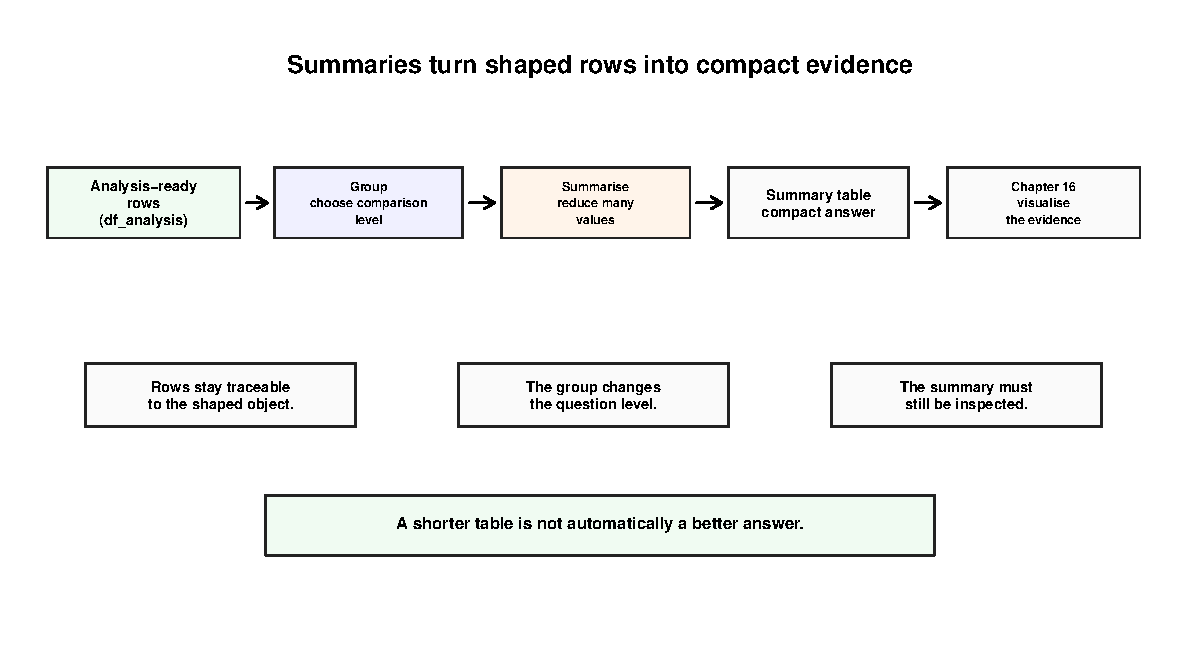
\includegraphics[width=0.9\linewidth,height=\textheight,keepaspectratio]{chapters/15-summarising-and-grouping-data_files/figure-pdf/fig-analysis-to-summary-evidence-1.pdf}

}

\caption{\label{fig-analysis-to-summary-evidence}From Analysis-Ready
Rows to Summary Evidence}

\end{figure}%

As shown in Figure~\ref{fig-analysis-to-summary-evidence}, Chapter 15
does not return to raw data and does not yet create analytical data
plots. It reduces shaped rows into summary evidence. The summary table
then becomes something Chapter 16 can visualise.

The order matters. A chart built from a poor summary only makes the
problem easier to see.

\section{Summarising and Grouping Are Different
Moves}\label{summarising-and-grouping-are-different-moves}

Summarising and grouping often appear together, but they are not the
same action.

\begin{longtable}[]{@{}
  >{\raggedright\arraybackslash}p{(\linewidth - 6\tabcolsep) * \real{0.2500}}
  >{\raggedright\arraybackslash}p{(\linewidth - 6\tabcolsep) * \real{0.2500}}
  >{\raggedright\arraybackslash}p{(\linewidth - 6\tabcolsep) * \real{0.2500}}
  >{\raggedright\arraybackslash}p{(\linewidth - 6\tabcolsep) * \real{0.2500}}@{}}
\caption{Core summary and grouping moves in Chapter
15}\label{tbl-summary-grouping-moves}\tabularnewline
\toprule\noalign{}
\begin{minipage}[b]{\linewidth}\raggedright
Move
\end{minipage} & \begin{minipage}[b]{\linewidth}\raggedright
Main question
\end{minipage} & \begin{minipage}[b]{\linewidth}\raggedright
Base R pattern
\end{minipage} & \begin{minipage}[b]{\linewidth}\raggedright
Tidyverse pattern
\end{minipage} \\
\midrule\noalign{}
\endfirsthead
\toprule\noalign{}
\begin{minipage}[b]{\linewidth}\raggedright
Move
\end{minipage} & \begin{minipage}[b]{\linewidth}\raggedright
Main question
\end{minipage} & \begin{minipage}[b]{\linewidth}\raggedright
Base R pattern
\end{minipage} & \begin{minipage}[b]{\linewidth}\raggedright
Tidyverse pattern
\end{minipage} \\
\midrule\noalign{}
\endhead
\bottomrule\noalign{}
\endlastfoot
Count rows & How many observations are present? & \texttt{nrow(df)} &
\texttt{summarise(n\ =\ n())} \\
Count categories & How many observations per category? &
\texttt{table(df\$x)} & \texttt{count(x)} \\
Summarise one variable & What is the centre or spread? &
\texttt{mean(df\$x,\ na.rm\ =\ TRUE)} &
\texttt{summarise(mean\_x\ =\ mean(x,\ na.rm\ =\ TRUE))} \\
Grouped summary & How does a measure differ by group? &
\texttt{aggregate(y\ \textasciitilde{}\ group,\ data\ =\ df,\ FUN\ =\ mean)}
& \texttt{group\_by(group)} then \texttt{summarise(...)} \\
Logical proportion & What share meets a condition? &
\texttt{mean(df\$flag,\ na.rm\ =\ TRUE)} &
\texttt{summarise(prop\ =\ mean(flag,\ na.rm\ =\ TRUE))} \\
Ungroup or drop groups & Should later work return to ordinary rows? &
Use an ungrouped object & \texttt{.groups\ =\ "drop"} or
\texttt{ungroup()} \\
\end{longtable}

The distinction in Table~\ref{tbl-summary-grouping-moves} helps Leo
avoid a common mistake.

A summary function such as \texttt{mean()} reduces values. A grouping
variable such as \texttt{background} or \texttt{study\_band} decides
where separate reductions should happen.

So this question:

\begin{Shaded}
\begin{Highlighting}[]
\NormalTok{What is the mean project score?}
\end{Highlighting}
\end{Shaded}

is not the same as this question:

\begin{Shaded}
\begin{Highlighting}[]
\NormalTok{What is the mean project score by background?}
\end{Highlighting}
\end{Shaded}

The second question changes the level of analysis.

\section{Summary Questions Come Before Summary
Code}\label{summary-questions-come-before-summary-code}

Before writing summary code, Leo should name the question.

That habit prevents empty calculation. It also makes the summary easier
to inspect.

A few useful questions for \texttt{df\_analysis} are:

\begin{Shaded}
\begin{Highlighting}[]
\NormalTok{How many observations are in the shaped data?}
\NormalTok{What is the mean project score?}
\NormalTok{What is the median project score?}
\NormalTok{How many observations show that the first script was completed?}
\NormalTok{What proportion reached a high project score?}
\NormalTok{How does mean project score differ by background?}
\NormalTok{How does mean project score differ by study band?}
\end{Highlighting}
\end{Shaded}

Each question requires a summary move.

Some questions count. Some calculate a centre. Some compare groups. Some
summarise a logical flag. Some need missing values handled deliberately.

\begin{tcolorbox}[enhanced jigsaw, arc=.35mm, bottomrule=.15mm, breakable, colback=white, colframe=quarto-callout-important-color-frame, left=2mm, leftrule=.75mm, opacityback=0, rightrule=.15mm, toprule=.15mm]
\begin{minipage}[t]{5.5mm}
\textcolor{quarto-callout-important-color}{\faExclamation}
\end{minipage}%
\begin{minipage}[t]{\textwidth - 5.5mm}

\vspace{-3mm}\textbf{Reliable Analysis Rule}\vspace{3mm}

A summary is not trustworthy because it is short. It becomes trustworthy
when Leo can explain what was counted, what was grouped, what was
excluded, and why the result answers the question.

\end{minipage}%
\end{tcolorbox}

\section{Counting Rows}\label{counting-rows}

The simplest summary asks how many observations are present.

In Base R:

\begin{Shaded}
\begin{Highlighting}[]
\FunctionTok{nrow}\NormalTok{(df\_analysis)}
\end{Highlighting}
\end{Shaded}

In tidyverse style:

\begin{Shaded}
\begin{Highlighting}[]
\NormalTok{df\_analysis }\SpecialCharTok{|\textgreater{}}
\NormalTok{  dplyr}\SpecialCharTok{::}\FunctionTok{summarise}\NormalTok{(}
    \AttributeTok{observations =}\NormalTok{ dplyr}\SpecialCharTok{::}\FunctionTok{n}\NormalTok{()}
\NormalTok{  )}
\end{Highlighting}
\end{Shaded}

These two examples do similar work, but they return results in different
forms. \texttt{nrow()} returns a single number. \texttt{summarise()}
returns a small table.

Leo should also remember that rows are observations, not always unique
learners. If the shaped data contains repeated learner-week records,
\texttt{nrow(df\_analysis)} counts observations. To count unique
learners, he would need a different summary:

\begin{Shaded}
\begin{Highlighting}[]
\NormalTok{df\_analysis }\SpecialCharTok{|\textgreater{}}
\NormalTok{  dplyr}\SpecialCharTok{::}\FunctionTok{summarise}\NormalTok{(}
    \AttributeTok{unique\_learners =}\NormalTok{ dplyr}\SpecialCharTok{::}\FunctionTok{n\_distinct}\NormalTok{(learner\_id)}
\NormalTok{  )}
\end{Highlighting}
\end{Shaded}

Leo should also remember that rows are observations, not always unique
learners. If the shaped data contains repeated learner-week records,
\texttt{nrow(df\_analysis)} counts observations. To count unique
learners, he would need a different summary:

\begin{Shaded}
\begin{Highlighting}[]
\NormalTok{df\_analysis }\SpecialCharTok{|\textgreater{}}
\NormalTok{  dplyr}\SpecialCharTok{::}\FunctionTok{summarise}\NormalTok{(}
    \AttributeTok{unique\_learners =}\NormalTok{ dplyr}\SpecialCharTok{::}\FunctionTok{n\_distinct}\NormalTok{(learner\_id)}
\NormalTok{  )}
\end{Highlighting}
\end{Shaded}

That difference matters later. A single number is useful in the console.
A small table is often easier to carry forward into a workflow.

\section{Summarising One Variable}\label{summarising-one-variable}

Leo may want to know the centre of a numeric variable such as
\texttt{project\_score}.

In Base R:

\begin{Shaded}
\begin{Highlighting}[]
\FunctionTok{mean}\NormalTok{(df\_analysis}\SpecialCharTok{$}\NormalTok{project\_score, }\AttributeTok{na.rm =} \ConstantTok{TRUE}\NormalTok{)}
\FunctionTok{median}\NormalTok{(df\_analysis}\SpecialCharTok{$}\NormalTok{project\_score, }\AttributeTok{na.rm =} \ConstantTok{TRUE}\NormalTok{)}
\FunctionTok{min}\NormalTok{(df\_analysis}\SpecialCharTok{$}\NormalTok{project\_score, }\AttributeTok{na.rm =} \ConstantTok{TRUE}\NormalTok{)}
\FunctionTok{max}\NormalTok{(df\_analysis}\SpecialCharTok{$}\NormalTok{project\_score, }\AttributeTok{na.rm =} \ConstantTok{TRUE}\NormalTok{)}
\end{Highlighting}
\end{Shaded}

In tidyverse style:

\begin{Shaded}
\begin{Highlighting}[]
\NormalTok{df\_analysis }\SpecialCharTok{|\textgreater{}}
\NormalTok{  dplyr}\SpecialCharTok{::}\FunctionTok{summarise}\NormalTok{(}
    \AttributeTok{mean\_project\_score =} \FunctionTok{mean}\NormalTok{(project\_score, }\AttributeTok{na.rm =} \ConstantTok{TRUE}\NormalTok{),}
    \AttributeTok{median\_project\_score =} \FunctionTok{median}\NormalTok{(project\_score, }\AttributeTok{na.rm =} \ConstantTok{TRUE}\NormalTok{),}
    \AttributeTok{min\_project\_score =} \FunctionTok{min}\NormalTok{(project\_score, }\AttributeTok{na.rm =} \ConstantTok{TRUE}\NormalTok{),}
    \AttributeTok{max\_project\_score =} \FunctionTok{max}\NormalTok{(project\_score, }\AttributeTok{na.rm =} \ConstantTok{TRUE}\NormalTok{)}
\NormalTok{  )}
\end{Highlighting}
\end{Shaded}

The tidyverse version is longer, but it names each result. That naming
matters because a summary table should explain itself.

Leo can use the same pattern for \texttt{study\_hours},
\texttt{lessons\_completed}, or \texttt{score\_gap}:

\begin{Shaded}
\begin{Highlighting}[]
\NormalTok{df\_analysis }\SpecialCharTok{|\textgreater{}}
\NormalTok{  dplyr}\SpecialCharTok{::}\FunctionTok{summarise}\NormalTok{(}
    \AttributeTok{mean\_study\_hours =} \FunctionTok{mean}\NormalTok{(study\_hours, }\AttributeTok{na.rm =} \ConstantTok{TRUE}\NormalTok{),}
    \AttributeTok{mean\_lessons\_completed =} \FunctionTok{mean}\NormalTok{(lessons\_completed, }\AttributeTok{na.rm =} \ConstantTok{TRUE}\NormalTok{),}
    \AttributeTok{mean\_score\_gap =} \FunctionTok{mean}\NormalTok{(score\_gap, }\AttributeTok{na.rm =} \ConstantTok{TRUE}\NormalTok{)}
\NormalTok{  )}
\end{Highlighting}
\end{Shaded}

The code is not just calculation. It is a set of named answers.

\section{Missing Values in Summaries}\label{missing-values-in-summaries}

Missing values can change a summary immediately.

If Leo writes:

\begin{Shaded}
\begin{Highlighting}[]
\FunctionTok{mean}\NormalTok{(df\_analysis}\SpecialCharTok{$}\NormalTok{project\_score)}
\end{Highlighting}
\end{Shaded}

and \texttt{project\_score} contains \texttt{NA}, R returns \texttt{NA}.
R is following the logic of missingness. It will not pretend that an
unknown value is known.

A common response is to add \texttt{na.rm\ =\ TRUE}:

\begin{Shaded}
\begin{Highlighting}[]
\FunctionTok{mean}\NormalTok{(df\_analysis}\SpecialCharTok{$}\NormalTok{project\_score, }\AttributeTok{na.rm =} \ConstantTok{TRUE}\NormalTok{)}
\end{Highlighting}
\end{Shaded}

That tells R to remove missing values for the purpose of that
calculation.

But this line needs a warning.

\begin{quote}
\texttt{na.rm\ =\ TRUE} tells R how to calculate around missing values.
It does not explain why the values are missing.
\end{quote}

So Leo should inspect missingness before relying on the summary:

\begin{Shaded}
\begin{Highlighting}[]
\FunctionTok{sum}\NormalTok{(}\FunctionTok{is.na}\NormalTok{(df\_analysis}\SpecialCharTok{$}\NormalTok{project\_score))}
\end{Highlighting}
\end{Shaded}

In tidyverse style:

\begin{Shaded}
\begin{Highlighting}[]
\NormalTok{df\_analysis }\SpecialCharTok{|\textgreater{}}
\NormalTok{  dplyr}\SpecialCharTok{::}\FunctionTok{summarise}\NormalTok{(}
    \AttributeTok{missing\_project\_score =} \FunctionTok{sum}\NormalTok{(}\FunctionTok{is.na}\NormalTok{(project\_score)),}
    \AttributeTok{observed\_project\_score =} \FunctionTok{sum}\NormalTok{(}\SpecialCharTok{!}\FunctionTok{is.na}\NormalTok{(project\_score)),}
    \AttributeTok{mean\_project\_score =} \FunctionTok{mean}\NormalTok{(project\_score, }\AttributeTok{na.rm =} \ConstantTok{TRUE}\NormalTok{)}
\NormalTok{  )}
\end{Highlighting}
\end{Shaded}

This is better than calculating the mean alone because it gives the
summary some context. Leo can see how many values were available for the
calculation.

\section{Counting Categories}\label{counting-categories}

Some variables are categorical. Leo may want to count them rather than
average them.

For example, \texttt{completion\_status} is not a score. It is a
category. The useful question is not:

\begin{Shaded}
\begin{Highlighting}[]
\NormalTok{What is the mean completion status?}
\end{Highlighting}
\end{Shaded}

The useful question is:

\begin{Shaded}
\begin{Highlighting}[]
\NormalTok{How many observations fall into each completion status?}
\end{Highlighting}
\end{Shaded}

In Base R:

\begin{Shaded}
\begin{Highlighting}[]
\FunctionTok{table}\NormalTok{(df\_analysis}\SpecialCharTok{$}\NormalTok{completion\_status, }\AttributeTok{useNA =} \StringTok{"ifany"}\NormalTok{)}
\end{Highlighting}
\end{Shaded}

In tidyverse style:

\begin{Shaded}
\begin{Highlighting}[]
\NormalTok{df\_analysis }\SpecialCharTok{|\textgreater{}}
\NormalTok{  dplyr}\SpecialCharTok{::}\FunctionTok{count}\NormalTok{(completion\_status)}
\end{Highlighting}
\end{Shaded}

Other useful category counts may involve \texttt{background},
\texttt{country}, \texttt{r\_experience\_level}, \texttt{study\_band},
or \texttt{first\_script\_completed}.

\begin{Shaded}
\begin{Highlighting}[]
\NormalTok{df\_analysis }\SpecialCharTok{|\textgreater{}}
\NormalTok{  dplyr}\SpecialCharTok{::}\FunctionTok{count}\NormalTok{(background)}

\NormalTok{df\_analysis }\SpecialCharTok{|\textgreater{}}
\NormalTok{  dplyr}\SpecialCharTok{::}\FunctionTok{count}\NormalTok{(study\_band)}

\NormalTok{df\_analysis }\SpecialCharTok{|\textgreater{}}
\NormalTok{  dplyr}\SpecialCharTok{::}\FunctionTok{count}\NormalTok{(first\_script\_completed)}
\end{Highlighting}
\end{Shaded}

Counting categories is often the first serious way to understand the
shape of a dataset.

It is also a check against assumptions. If a category count produces
unexpected labels or missing values, Leo should not rush to explain them
away. He should inspect them.

\section{Grouping: Changing the Level of the
Question}\label{grouping-changing-the-level-of-the-question}

Grouping is one of the most important mental shifts in data work.

Without grouping, Leo asks one question about the whole analysis object:

\begin{Shaded}
\begin{Highlighting}[]
\NormalTok{What is the mean project score overall?}
\end{Highlighting}
\end{Shaded}

With grouping, he asks the same question separately within categories:

\begin{Shaded}
\begin{Highlighting}[]
\NormalTok{What is the mean project score by background?}
\end{Highlighting}
\end{Shaded}

The measure may be the same. The level of the question changes.

That is why grouping matters.

Grouping does not magically make the analysis deeper. It makes the
comparison explicit.

\section{Grouped Summaries with Base
R}\label{grouped-summaries-with-base-r}

Base R can produce grouped summaries with \texttt{aggregate()}.

For example, to calculate mean project score by \texttt{background}:

\begin{Shaded}
\begin{Highlighting}[]
\FunctionTok{aggregate}\NormalTok{(}
\NormalTok{  project\_score }\SpecialCharTok{\textasciitilde{}}\NormalTok{ background,}
  \AttributeTok{data =}\NormalTok{ df\_analysis,}
  \AttributeTok{FUN =} \ControlFlowTok{function}\NormalTok{(x) }\FunctionTok{mean}\NormalTok{(x, }\AttributeTok{na.rm =} \ConstantTok{TRUE}\NormalTok{)}
\NormalTok{)}
\end{Highlighting}
\end{Shaded}

The formula \texttt{project\_score\ \textasciitilde{}\ background} can
be read as:

\begin{Shaded}
\begin{Highlighting}[]
\NormalTok{Summarise project\_score by background.}
\end{Highlighting}
\end{Shaded}

This is a compact expression. It is useful, but beginners should read it
slowly. The variable on the left is the measure. The variable on the
right is the group.

Leo can also use \texttt{tapply()} for simple grouped summaries:

\begin{Shaded}
\begin{Highlighting}[]
\FunctionTok{tapply}\NormalTok{(}
\NormalTok{  df\_analysis}\SpecialCharTok{$}\NormalTok{project\_score,}
\NormalTok{  df\_analysis}\SpecialCharTok{$}\NormalTok{background,}
\NormalTok{  mean,}
  \AttributeTok{na.rm =} \ConstantTok{TRUE}
\NormalTok{)}
\end{Highlighting}
\end{Shaded}

Both approaches are useful. The purpose here is not to memorise every
Base R summary tool. The purpose is to see that grouped summaries are
not exclusive to one style of R.

\section{Grouped Summaries with
Tidyverse}\label{grouped-summaries-with-tidyverse}

In tidyverse style, Leo usually writes the grouping step explicitly:

\begin{Shaded}
\begin{Highlighting}[]
\NormalTok{df\_analysis }\SpecialCharTok{|\textgreater{}}
\NormalTok{  dplyr}\SpecialCharTok{::}\FunctionTok{group\_by}\NormalTok{(background) }\SpecialCharTok{|\textgreater{}}
\NormalTok{  dplyr}\SpecialCharTok{::}\FunctionTok{summarise}\NormalTok{(}
    \AttributeTok{observations =}\NormalTok{ dplyr}\SpecialCharTok{::}\FunctionTok{n}\NormalTok{(),}
    \AttributeTok{mean\_project\_score =} \FunctionTok{mean}\NormalTok{(project\_score, }\AttributeTok{na.rm =} \ConstantTok{TRUE}\NormalTok{),}
    \AttributeTok{median\_project\_score =} \FunctionTok{median}\NormalTok{(project\_score, }\AttributeTok{na.rm =} \ConstantTok{TRUE}\NormalTok{),}
    \AttributeTok{.groups =} \StringTok{"drop"}
\NormalTok{  )}
\end{Highlighting}
\end{Shaded}

This code has a readable structure.

\texttt{group\_by(background)} tells R to create separate groups.
\texttt{summarise()} tells R what to calculate inside those groups.
\texttt{.groups\ =\ "drop"} tells R to return an ordinary ungrouped
summary table after the calculation.

That last part may look small, but it is a useful habit. Grouping can
remain attached to a result in tidyverse workflows. Dropping groups when
they are no longer needed helps avoid confusion later.

\begin{tcolorbox}[enhanced jigsaw, arc=.35mm, bottomrule=.15mm, breakable, colback=white, colframe=quarto-callout-tip-color-frame, left=2mm, leftrule=.75mm, opacityback=0, rightrule=.15mm, toprule=.15mm]
\begin{minipage}[t]{5.5mm}
\textcolor{quarto-callout-tip-color}{\faLightbulb}
\end{minipage}%
\begin{minipage}[t]{\textwidth - 5.5mm}

\vspace{-3mm}\textbf{How R Thinks}\vspace{3mm}

In a grouped summary, R does not calculate one overall result first. It
splits the data into groups, applies the summary action inside each
group, and then returns a smaller table of results.

\end{minipage}%
\end{tcolorbox}

\section{Two-Group Comparisons}\label{two-group-comparisons}

Sometimes one grouping variable is enough. Other times Leo may need two.

For example, he may ask:

\begin{Shaded}
\begin{Highlighting}[]
\NormalTok{How does project performance differ by background and study band?}
\end{Highlighting}
\end{Shaded}

In tidyverse style:

\begin{Shaded}
\begin{Highlighting}[]
\NormalTok{df\_analysis }\SpecialCharTok{|\textgreater{}}
\NormalTok{  dplyr}\SpecialCharTok{::}\FunctionTok{group\_by}\NormalTok{(background, study\_band) }\SpecialCharTok{|\textgreater{}}
\NormalTok{  dplyr}\SpecialCharTok{::}\FunctionTok{summarise}\NormalTok{(}
    \AttributeTok{observations =}\NormalTok{ dplyr}\SpecialCharTok{::}\FunctionTok{n}\NormalTok{(),}
    \AttributeTok{mean\_project\_score =} \FunctionTok{mean}\NormalTok{(project\_score, }\AttributeTok{na.rm =} \ConstantTok{TRUE}\NormalTok{),}
    \AttributeTok{mean\_score\_gap =} \FunctionTok{mean}\NormalTok{(score\_gap, }\AttributeTok{na.rm =} \ConstantTok{TRUE}\NormalTok{),}
    \AttributeTok{.groups =} \StringTok{"drop"}
\NormalTok{  )}
\end{Highlighting}
\end{Shaded}

This can be useful, but it should be used carefully.

Every extra grouping variable divides the data into smaller pieces. Some
groups may become too small to interpret responsibly.

Leo should inspect group sizes:

\begin{Shaded}
\begin{Highlighting}[]
\NormalTok{df\_analysis }\SpecialCharTok{|\textgreater{}}
\NormalTok{  dplyr}\SpecialCharTok{::}\FunctionTok{count}\NormalTok{(background, study\_band)}
\end{Highlighting}
\end{Shaded}

If a group has very few observations, the summary may be unstable. The
number may still calculate, but that does not make it meaningful.

\section{Proportions and Logical
Summaries}\label{proportions-and-logical-summaries}

Chapter 7 taught Leo that logical values are real values: \texttt{TRUE}
and \texttt{FALSE}.

In summaries, that becomes powerful. In R, \texttt{TRUE} behaves like
\texttt{1} and \texttt{FALSE} behaves like \texttt{0} inside numeric
calculations such as \texttt{mean()}.

That means Leo can calculate a proportion from a logical variable.

For example, if \texttt{high\_project\_score} is \texttt{TRUE} when
\texttt{project\_score\ \textgreater{}=\ 80}, then:

\begin{Shaded}
\begin{Highlighting}[]
\FunctionTok{mean}\NormalTok{(df\_analysis}\SpecialCharTok{$}\NormalTok{high\_project\_score, }\AttributeTok{na.rm =} \ConstantTok{TRUE}\NormalTok{)}
\end{Highlighting}
\end{Shaded}

returns the proportion of observations with high project scores.

The tidyverse version is:

\begin{Shaded}
\begin{Highlighting}[]
\NormalTok{df\_analysis }\SpecialCharTok{|\textgreater{}}
\NormalTok{  dplyr}\SpecialCharTok{::}\FunctionTok{summarise}\NormalTok{(}
    \AttributeTok{proportion\_high\_project\_score =} \FunctionTok{mean}\NormalTok{(high\_project\_score, }\AttributeTok{na.rm =} \ConstantTok{TRUE}\NormalTok{)}
\NormalTok{  )}
\end{Highlighting}
\end{Shaded}

The same idea works for logical fields such as
\texttt{first\_script\_completed}, \texttt{used\_quarto}, and
\texttt{used\_git}:

\begin{Shaded}
\begin{Highlighting}[]
\NormalTok{df\_analysis }\SpecialCharTok{|\textgreater{}}
\NormalTok{  dplyr}\SpecialCharTok{::}\FunctionTok{summarise}\NormalTok{(}
    \AttributeTok{proportion\_first\_script\_completed =} \FunctionTok{mean}\NormalTok{(first\_script\_completed, }\AttributeTok{na.rm =} \ConstantTok{TRUE}\NormalTok{),}
    \AttributeTok{proportion\_used\_quarto =} \FunctionTok{mean}\NormalTok{(used\_quarto, }\AttributeTok{na.rm =} \ConstantTok{TRUE}\NormalTok{),}
    \AttributeTok{proportion\_used\_git =} \FunctionTok{mean}\NormalTok{(used\_git, }\AttributeTok{na.rm =} \ConstantTok{TRUE}\NormalTok{)}
\NormalTok{  )}
\end{Highlighting}
\end{Shaded}

This is not a trick. It is Chapter 7 becoming useful inside a workflow.
Logical judgments can become summary evidence.

\section{Grouped Proportions}\label{grouped-proportions}

Leo can also calculate proportions inside groups.

In Base R, one simple option is \texttt{aggregate()}:

\begin{Shaded}
\begin{Highlighting}[]
\FunctionTok{aggregate}\NormalTok{(}
\NormalTok{  high\_project\_score }\SpecialCharTok{\textasciitilde{}}\NormalTok{ background,}
  \AttributeTok{data =}\NormalTok{ df\_analysis,}
  \AttributeTok{FUN =} \ControlFlowTok{function}\NormalTok{(x) }\FunctionTok{mean}\NormalTok{(x, }\AttributeTok{na.rm =} \ConstantTok{TRUE}\NormalTok{)}
\NormalTok{)}
\end{Highlighting}
\end{Shaded}

The result gives the proportion of TRUE values for
\texttt{high\_project\_score} inside each background group.

In tidyverse style:

\begin{Shaded}
\begin{Highlighting}[]
\NormalTok{df\_analysis }\SpecialCharTok{|\textgreater{}}
\NormalTok{  dplyr}\SpecialCharTok{::}\FunctionTok{group\_by}\NormalTok{(background) }\SpecialCharTok{|\textgreater{}}
\NormalTok{  dplyr}\SpecialCharTok{::}\FunctionTok{summarise}\NormalTok{(}
    \AttributeTok{observations =}\NormalTok{ dplyr}\SpecialCharTok{::}\FunctionTok{n}\NormalTok{(),}
    \AttributeTok{proportion\_high\_project\_score =} \FunctionTok{mean}\NormalTok{(high\_project\_score, }\AttributeTok{na.rm =} \ConstantTok{TRUE}\NormalTok{),}
    \AttributeTok{proportion\_first\_script\_completed =} \FunctionTok{mean}\NormalTok{(first\_script\_completed, }\AttributeTok{na.rm =} \ConstantTok{TRUE}\NormalTok{),}
    \AttributeTok{.groups =} \StringTok{"drop"}
\NormalTok{  )}
\end{Highlighting}
\end{Shaded}

This summary asks:

\begin{Shaded}
\begin{Highlighting}[]
\NormalTok{Within each background group, what proportion reached a high project score and completed the first script?}
\end{Highlighting}
\end{Shaded}

That is more meaningful than one overall proportion if Leo wants to
compare learner backgrounds.

But the same warning still applies. A grouped proportion should be
interpreted alongside group size.

\section{Summary Tables Need
Inspection}\label{summary-tables-need-inspection}

A summary table is not automatically trustworthy.

Leo should inspect it just as he inspected imported, cleaned, and shaped
data.

For example:

\begin{Shaded}
\begin{Highlighting}[]
\NormalTok{summary\_by\_background }\OtherTok{\textless{}{-}}\NormalTok{ df\_analysis }\SpecialCharTok{|\textgreater{}}
\NormalTok{  dplyr}\SpecialCharTok{::}\FunctionTok{group\_by}\NormalTok{(background) }\SpecialCharTok{|\textgreater{}}
\NormalTok{  dplyr}\SpecialCharTok{::}\FunctionTok{summarise}\NormalTok{(}
    \AttributeTok{observations =}\NormalTok{ dplyr}\SpecialCharTok{::}\FunctionTok{n}\NormalTok{(),}
    \AttributeTok{mean\_project\_score =} \FunctionTok{mean}\NormalTok{(project\_score, }\AttributeTok{na.rm =} \ConstantTok{TRUE}\NormalTok{),}
    \AttributeTok{median\_project\_score =} \FunctionTok{median}\NormalTok{(project\_score, }\AttributeTok{na.rm =} \ConstantTok{TRUE}\NormalTok{),}
    \AttributeTok{mean\_score\_gap =} \FunctionTok{mean}\NormalTok{(score\_gap, }\AttributeTok{na.rm =} \ConstantTok{TRUE}\NormalTok{),}
    \AttributeTok{proportion\_high\_project\_score =} \FunctionTok{mean}\NormalTok{(high\_project\_score, }\AttributeTok{na.rm =} \ConstantTok{TRUE}\NormalTok{),}
    \AttributeTok{.groups =} \StringTok{"drop"}
\NormalTok{  )}
\end{Highlighting}
\end{Shaded}

Then inspect:

\begin{Shaded}
\begin{Highlighting}[]
\NormalTok{summary\_by\_background}
\FunctionTok{dim}\NormalTok{(summary\_by\_background)}
\FunctionTok{names}\NormalTok{(summary\_by\_background)}
\FunctionTok{str}\NormalTok{(summary\_by\_background)}
\end{Highlighting}
\end{Shaded}

These checks may feel simple, but they keep the workflow honest.

Leo should ask:

\begin{Shaded}
\begin{Highlighting}[]
\NormalTok{Are the groups what I expected?}
\NormalTok{Are the counts large enough to interpret?}
\NormalTok{Are missing values handled deliberately?}
\NormalTok{Do the column names explain the summary?}
\NormalTok{Does this summary answer the question I asked?}
\end{Highlighting}
\end{Shaded}

If the answer is unclear, the solution is not to make a prettier table.
The solution is to return to the question, the data, or the summary
logic.

\section{Summary Objects for Chapter
16}\label{summary-objects-for-chapter-16}

Chapter 15 should leave Leo with one or two summary objects that can be
visualised later.

The first object is the summary already created and inspected:

\begin{Shaded}
\begin{Highlighting}[]
\NormalTok{summary\_by\_background}
\end{Highlighting}
\end{Shaded}

That object compares project performance across learner backgrounds.

A second useful object is:

\begin{Shaded}
\begin{Highlighting}[]
\CommentTok{\#| eval: false}
\NormalTok{summary\_by\_study\_band}
\end{Highlighting}
\end{Shaded}

For example:

\begin{Shaded}
\begin{Highlighting}[]
\CommentTok{\#| eval: false}
\NormalTok{summary\_by\_study\_band }\OtherTok{\textless{}{-}}\NormalTok{ df\_analysis }\SpecialCharTok{|\textgreater{}}
\NormalTok{  dplyr}\SpecialCharTok{::}\FunctionTok{group\_by}\NormalTok{(study\_band) }\SpecialCharTok{|\textgreater{}}
\NormalTok{  dplyr}\SpecialCharTok{::}\FunctionTok{summarise}\NormalTok{(}
    \AttributeTok{observations =}\NormalTok{ dplyr}\SpecialCharTok{::}\FunctionTok{n}\NormalTok{(),}
    \AttributeTok{mean\_project\_score =} \FunctionTok{mean}\NormalTok{(project\_score, }\AttributeTok{na.rm =} \ConstantTok{TRUE}\NormalTok{),}
    \AttributeTok{mean\_score\_gap =} \FunctionTok{mean}\NormalTok{(score\_gap, }\AttributeTok{na.rm =} \ConstantTok{TRUE}\NormalTok{),}
    \AttributeTok{proportion\_high\_project\_score =} \FunctionTok{mean}\NormalTok{(high\_project\_score, }\AttributeTok{na.rm =} \ConstantTok{TRUE}\NormalTok{),}
    \AttributeTok{.groups =} \StringTok{"drop"}
\NormalTok{  )}
\end{Highlighting}
\end{Shaded}

These objects are not final conclusions. They are summary evidence.
Chapter 16 will ask how to visualise evidence like this without
distorting what it means.

\section{Common Beginner Mistakes}\label{common-beginner-mistakes-7}

\subsection{Mistake 1: Summarising before asking a
question}\label{mistake-1-summarising-before-asking-a-question}

A summary should answer something.

If Leo calculates every possible mean, median, count, and proportion, he
has not necessarily analysed the data. He has produced noise in
numerical form.

The question comes first.

\subsection{\texorpdfstring{Mistake 2: Treating \texttt{na.rm\ =\ TRUE}
as a
solution}{Mistake 2: Treating na.rm = TRUE as a solution}}\label{mistake-2-treating-na.rm-true-as-a-solution}

\texttt{na.rm\ =\ TRUE} helps R calculate around missing values. It does
not explain why the missing values exist.

Leo should count missing values before deciding how to summarise around
them.

\subsection{Mistake 3: Grouping by too many variables too
soon}\label{mistake-3-grouping-by-too-many-variables-too-soon}

A summary by \texttt{background}, \texttt{country},
\texttt{study\_band}, and \texttt{completion\_status} may produce many
tiny groups.

That can make the summary look detailed while weakening its
interpretability.

\subsection{Mistake 4: Forgetting that grouping changes the level of
analysis}\label{mistake-4-forgetting-that-grouping-changes-the-level-of-analysis}

An overall mean and a grouped mean answer different questions.

Leo should be able to say what level each summary represents.

\subsection{Mistake 5: Confusing filtering with
grouping}\label{mistake-5-confusing-filtering-with-grouping}

Filtering chooses which rows remain.

Grouping keeps rows but organises them into comparison categories before
summarising.

\subsection{Mistake 6: Trusting a summary because it looks
clean}\label{mistake-6-trusting-a-summary-because-it-looks-clean}

A clean summary table can still be misleading if the grouping,
missing-value handling, or original question is unclear.

\subsection{Mistake 7: Trying to visualise before understanding the
summary}\label{mistake-7-trying-to-visualise-before-understanding-the-summary}

Visualisation can make a weak summary more persuasive than it deserves.

Chapter 16 will teach visualisation, but Chapter 15 must first make sure
the summary evidence is worth visualising.

\section{What Leo Is Expected to Know at This
Point}\label{what-leo-is-expected-to-know-at-this-point-8}

By the end of this chapter, Leo should be able to explain the difference
between summarising and grouping. He should know how to count
observations, calculate simple numeric summaries, count categories,
calculate proportions from logical variables, and compare summaries
across groups.

He should also know that summaries need inspection. A summary table is
smaller than the data, but it is not automatically more truthful.

\begin{tcolorbox}[enhanced jigsaw, arc=.35mm, bottomrule=.15mm, breakable, colback=white, colframe=quarto-callout-note-color-frame, left=2mm, leftrule=.75mm, opacityback=0, rightrule=.15mm, toprule=.15mm]
\begin{minipage}[t]{5.5mm}
\textcolor{quarto-callout-note-color}{\faInfo}
\end{minipage}%
\begin{minipage}[t]{\textwidth - 5.5mm}

\vspace{-3mm}\textbf{Not Yet}\vspace{3mm}

Leo is not expected to create visualisations in this chapter. He is not
expected to model relationships, test hypotheses, or build reports.

Chapter 15 ends when Leo knows how to turn shaped rows into summary
evidence that can be inspected, explained, and later visualised.

\end{minipage}%
\end{tcolorbox}

\section{Chapter Outcome}\label{chapter-outcome-14}

Chapter 15 has shown Leo how to move from analysis-ready rows to summary
evidence.

He can now count observations, summarise numeric variables, count
categories, calculate simple proportions, group by meaningful variables,
and inspect the resulting summary tables.

More importantly, he understands that summaries are choices.

A summary depends on the question, the grouping level, the variables
selected, the missing values removed or retained, and the logic used to
create the shaped data. That makes summary work powerful, but it also
makes it responsible.

The object \texttt{df\_analysis} gives Leo shaped rows. Summary objects
such as \texttt{summary\_by\_background} and
\texttt{summary\_by\_study\_band} show how those rows can become compact
evidence.

\section{Closing Part 3}\label{closing-part-3}

Part 3 began with a practical problem: Leo needed to move from knowing
R's language to doing data work with discipline.

The workflow was:

\begin{Shaded}
\begin{Highlighting}[]
\NormalTok{Packages {-}\textgreater{} Import {-}\textgreater{} Inspect {-}\textgreater{} Clean {-}\textgreater{} Transform {-}\textgreater{} Summarise}
\end{Highlighting}
\end{Shaded}

Chapter 11 prepared the package tools. Chapter 12 brought the official
dataset into R. Chapter 13 cleaned and prepared the evidence. Chapter 14
shaped it for analysis. Chapter 15 turned those shaped rows into summary
evidence, with grouping making comparison possible.

Leo has not merely learned commands. He has learned a workflow.

He now knows that serious data work is not a single heroic calculation.
It is a sequence of controlled moves: prepare the tools, import the
evidence, inspect what arrived, clean without hiding changes, shape the
data for a question, and summarise the result responsibly.

That is the close of Part 3: Leo has moved from tools and raw files to
prepared, shaped, and summarised evidence.

\section{\texorpdfstring{Saving \texttt{df\_analysis} for Part
4}{Saving df\_analysis for Part 4}}\label{saving-df_analysis-for-part-4}

Chapter 16 should not return to the raw CSV file as if Chapters 14 and
15 never happened. The raw file remains the source evidence, but the
object that now belongs to visualisation is the shaped analysis object:

\begin{Shaded}
\begin{Highlighting}[]
\NormalTok{df\_analysis}
\end{Highlighting}
\end{Shaded}

That object carries the analytical decisions Leo has already made:
selected variables, filtered observations, and derived variables such as
\texttt{high\_project\_score}, \texttt{score\_gap}, and
\texttt{study\_band}.

So before Part 4 begins, Leo saves \texttt{df\_analysis} as a reusable
file.

\begin{Shaded}
\begin{Highlighting}[]
\ControlFlowTok{if}\NormalTok{ (}\SpecialCharTok{!}\FunctionTok{exists}\NormalTok{(}\StringTok{"df\_analysis"}\NormalTok{)) \{}
  \FunctionTok{stop}\NormalTok{(}
    \StringTok{"Chapter 15 could not create df\_analysis. "}\NormalTok{,}
    \StringTok{"Confirm that data/raw/df\_r\_migration\_messy.csv exists, "}\NormalTok{,}
    \StringTok{"or provide data/processed/df\_analysis.csv before rendering."}
\NormalTok{  )}
\NormalTok{\}}

\FunctionTok{dir.create}\NormalTok{(}\StringTok{"data/processed"}\NormalTok{, }\AttributeTok{recursive =} \ConstantTok{TRUE}\NormalTok{, }\AttributeTok{showWarnings =} \ConstantTok{FALSE}\NormalTok{)}

\FunctionTok{saveRDS}\NormalTok{(}
\NormalTok{  df\_analysis,}
  \StringTok{"data/processed/df\_analysis.rds"}
\NormalTok{)}

\FunctionTok{write.csv}\NormalTok{(}
\NormalTok{  df\_analysis,}
  \StringTok{"data/processed/df\_analysis.csv"}\NormalTok{,}
  \AttributeTok{row.names =} \ConstantTok{FALSE}
\NormalTok{)}

\ControlFlowTok{if}\NormalTok{ (}\FunctionTok{requireNamespace}\NormalTok{(}\StringTok{"writexl"}\NormalTok{, }\AttributeTok{quietly =} \ConstantTok{TRUE}\NormalTok{)) \{}
\NormalTok{  writexl}\SpecialCharTok{::}\FunctionTok{write\_xlsx}\NormalTok{(}
\NormalTok{    df\_analysis,}
    \StringTok{"data/processed/df\_analysis.xlsx"}
\NormalTok{  )}
\NormalTok{\}}
\end{Highlighting}
\end{Shaded}

For the online book, the reusable Part 4 dataset should be made
available here:

\href{../data/processed/df_analysis.csv}{Download
\texttt{df\_analysis.csv}}

\href{../data/processed/df_analysis.xlsx}{Download
\texttt{df\_analysis.xlsx}}

\begin{tcolorbox}[enhanced jigsaw, arc=.35mm, bottomrule=.15mm, breakable, colback=white, colframe=quarto-callout-important-color-frame, left=2mm, leftrule=.75mm, opacityback=0, rightrule=.15mm, toprule=.15mm]
\begin{minipage}[t]{5.5mm}
\textcolor{quarto-callout-important-color}{\faExclamation}
\end{minipage}%
\begin{minipage}[t]{\textwidth - 5.5mm}

\vspace{-3mm}\textbf{Why this handoff matters}\vspace{3mm}

Part 4 should visualise \texttt{df\_analysis}, not the raw dataset.
Visualisation should continue the evidence trail built across Part 3
rather than silently restarting the workflow from the raw file.

\end{minipage}%
\end{tcolorbox}

\section{Transition to Chapter 16}\label{transition-to-chapter-16}

Leo now knows how to create summary tables that can be inspected,
explained, and traced back to \texttt{df\_analysis}.

But summaries are still tables.

Some patterns become clearer when they are visualised. Some comparisons
are easier to understand when readers can see them. Some results become
more persuasive when the visual form matches the evidence honestly and
does not exaggerate it.

That creates the next question:

\begin{quote}
How can Leo visualise evidence clearly without distorting what it means?
\end{quote}

\begin{tcolorbox}[enhanced jigsaw, arc=.35mm, bottomrule=.15mm, breakable, colback=white, colframe=quarto-callout-tip-color-frame, left=2mm, leftrule=.75mm, opacityback=0, rightrule=.15mm, toprule=.15mm]
\begin{minipage}[t]{5.5mm}
\textcolor{quarto-callout-tip-color}{\faLightbulb}
\end{minipage}%
\begin{minipage}[t]{\textwidth - 5.5mm}

\vspace{-3mm}\textbf{Ready for Visualisation}\vspace{3mm}

Chapter 15 has shown Leo how shaped rows become summary evidence.
Chapter 16 begins the next stage: visualising that evidence clearly,
responsibly, and without losing the trust built across Part 3.

\end{minipage}%
\end{tcolorbox}

\part{Part 4: Seeing and Communicating Insight}

\chapter{Data Visualization: Turning Patterns into
Pictures}\label{data-visualization-turning-patterns-into-pictures}

\renewcommand{\thefigure}{16.\arabic{figure}}
\setcounter{figure}{0}
\renewcommand{\thetable}{16.\arabic{table}}
\setcounter{table}{0}

\section{Opening Scene: When the Table Stops Being
Enough}\label{opening-scene-when-the-table-stops-being-enough}

Leo has reached an important point in the workflow.

In Chapter 11, he learned that serious R work depends on tools as well
as language. In Chapter 12, he moved the project dataset from a file on
disk into an R object. In Chapter 13, he learned that imported data must
be inspected and prepared before analysis. In Chapter 14, he selected,
filtered, and transformed rows into an analysis-ready form. In Chapter
15, he grouped and summarised those rows so that many observations could
speak together.

That is real progress.

For the first time, Leo can ask questions and get evidence back.

He can write:

\begin{codelisting}

\caption{\label{lst-chapter16-first-summary}Code for the First Grouped
Summary Used to Motivate Visualisation}

\centering{

\begin{Shaded}
\begin{Highlighting}[]
\NormalTok{df\_analysis }\SpecialCharTok{|\textgreater{}}
  \FunctionTok{group\_by}\NormalTok{(background) }\SpecialCharTok{|\textgreater{}}
  \FunctionTok{summarise}\NormalTok{(}
    \AttributeTok{learners =} \FunctionTok{n}\NormalTok{(),}
    \AttributeTok{avg\_project\_score =} \FunctionTok{mean}\NormalTok{(project\_score, }\AttributeTok{na.rm =} \ConstantTok{TRUE}\NormalTok{),}
    \AttributeTok{.groups =} \StringTok{"drop"}
\NormalTok{  ) }\SpecialCharTok{|\textgreater{}}
\NormalTok{  knitr}\SpecialCharTok{::}\FunctionTok{kable}\NormalTok{()}
\end{Highlighting}
\end{Shaded}

}

\end{codelisting}%

{

\begin{longtable}[]{@{}lrr@{}}

\caption{\label{tbl-16-first-grouped-summary}First Grouped Summary Used
to Motivate Visualisation}

\tabularnewline

\toprule\noalign{}
background & learners & avg\_project\_score \\
\midrule\noalign{}
\endhead
\bottomrule\noalign{}
\endlastfoot
Excel & 105 & 80.70571 \\
Google Sheets & 97 & 81.24124 \\
Manual Reporting & 54 & 78.12037 \\
Ms Excel & 66 & 81.66515 \\
Power Bi & 102 & 82.00931 \\
Spreadsheet & 160 & 80.48781 \\

\end{longtable}

}

The code in Listing~\ref{lst-chapter16-first-summary} creates
Table~\ref{tbl-16-first-grouped-summary}, the first grouped summary used
to motivate visualisation.

It is useful. It is precise. It is also slightly unsatisfying.

Leo reads the rows. He compares the numbers. He moves his eyes from one
category to another. He holds one average in memory while checking
another. He starts to understand the pattern, but the pattern has not
yet become visible.

That is the moment Chapter 16 begins.

A summary tells Leo what happened. A plot helps him see how the pattern
behaves.

The difference matters because professional analysis does not end with
correct numbers. Other people must be able to inspect the evidence,
notice the comparison, question the pattern, and understand the result
without fighting the format.

The central idea of this chapter is simple:

\begin{quote}
A good plot is not decoration. It is a visual argument built from data,
mappings, layers, scales, and design choices.
\end{quote}

This chapter opens Part 4 by moving Leo from data manipulation into
visual evidence. Chapter 17 will later help him refine that evidence for
clarity and control. Chapter 18 will help him connect plots into a
fuller story. For now, the work is more fundamental: Leo needs to learn
how a plot is built.

\begin{tcolorbox}[enhanced jigsaw, arc=.35mm, bottomrule=.15mm, breakable, colback=white, colframe=quarto-callout-note-color-frame, left=2mm, leftrule=.75mm, opacityback=0, rightrule=.15mm, toprule=.15mm]
\begin{minipage}[t]{5.5mm}
\textcolor{quarto-callout-note-color}{\faInfo}
\end{minipage}%
\begin{minipage}[t]{\textwidth - 5.5mm}

\vspace{-3mm}\textbf{Chapter Compass}\vspace{3mm}

In this chapter, Leo learns how to turn analysis-ready data into visual
evidence. He will meet base R graphics, recognise other plotting systems
he may encounter, and then focus on \texttt{ggplot2} because it gives
him a grammar for building plots from data, mappings, layers, scales,
facets, themes, and coordinates.

\end{minipage}%
\end{tcolorbox}

\section{Data Handoff from Part 3}\label{data-handoff-from-part-3}

Part 4 does not restart from the raw file. It continues from the
analysis-ready object created in Chapter 14 and carried through Chapter
15:

\begin{Shaded}
\begin{Highlighting}[]
\NormalTok{df\_analysis}
\end{Highlighting}
\end{Shaded}

The raw file, \texttt{df\_r\_migration\_messy.csv}, remains the source
evidence. But the visualisation chapters use the shaped data because
plotting should follow the same evidence trail Leo has already built.

To follow the Part 4 examples on his own machine, Leo needs the reusable
analysis-ready dataset created during the Chapter 15 handoff step. The
dataset is available in both CSV and Excel formats:

\href{../datasets/processed/df_analysis.csv}{Download
\texttt{df\_analysis.csv}}

\href{../datasets/processed/df_analysis.xlsx}{Download
\texttt{df\_analysis.xlsx}}

Place the CSV version in this project location before rendering Chapters
16 to 18:

\begin{Shaded}
\begin{Highlighting}[]
\NormalTok{data/processed/df\_analysis.csv}
\end{Highlighting}
\end{Shaded}

If that processed file is not present but the raw teaching dataset is
available at \texttt{data/raw/df\_r\_migration\_messy.csv}, the setup
chunk in this chapter rebuilds \texttt{df\_analysis} using the same Part
3 selection, filtering, and transformation logic. That fallback exists
for renderability; conceptually, the visualisation object remains
\texttt{df\_analysis}, not the raw dataset.

\begin{tcolorbox}[enhanced jigsaw, arc=.35mm, bottomrule=.15mm, breakable, colback=white, colframe=quarto-callout-important-color-frame, left=2mm, leftrule=.75mm, opacityback=0, rightrule=.15mm, toprule=.15mm]
\begin{minipage}[t]{5.5mm}
\textcolor{quarto-callout-important-color}{\faExclamation}
\end{minipage}%
\begin{minipage}[t]{\textwidth - 5.5mm}

\vspace{-3mm}\textbf{Why Chapter 16 uses df\_analysis}\vspace{3mm}

Visualisation should not silently return to raw data after the book has
already taught import, cleaning, shaping, and summarising. The correct
object for Part 4 is \texttt{df\_analysis}, because it is the
analysis-ready table produced by the Part 3 workflow.

\end{minipage}%
\end{tcolorbox}

\section{Why Visualization Comes After
Preparation}\label{why-visualization-comes-after-preparation}

A plot looks immediate. R draws it quickly, sometimes with one line of
code.

That speed can mislead beginners.

Visualization should not be treated as the first step in analysis. It
depends on everything Leo has already learned. A plot is only as
trustworthy as the data behind it.

If \texttt{project\_score} is still stored as text, a scatter plot will
fail or mislead. If \texttt{completion\_status} contains
\texttt{"Completed"}, \texttt{"completed\ "}, \texttt{"COMPLETE"}, and
\texttt{"Yes"} as separate categories, a bar chart will split one idea
into several bars. If missing values have not been recognised, a plot
may quietly remove rows. If rows are duplicated, a count plot may
exaggerate a group.

So visualization comes after importing, cleaning, transforming, and
summarising because plotting does not repair weak evidence. It reveals
the consequences of earlier decisions.

Chapter 16 therefore continues the same evidence trail:

\begin{codelisting}

\caption{\label{lst-chapter16-evidence-trail}Code for the Part 3
Evidence Trail Leading into Visualisation}

\centering{

\begin{Shaded}
\begin{Highlighting}[]
\NormalTok{raw\_migration              }\CommentTok{\# imported evidence}
\NormalTok{df\_r\_migration             }\CommentTok{\# working copy}
\NormalTok{df\_r\_migration\_prepared    }\CommentTok{\# cleaned and prepared evidence}
\NormalTok{df\_analysis                }\CommentTok{\# shaped analysis{-}ready evidence}
\end{Highlighting}
\end{Shaded}

}

\end{codelisting}%

The code in Listing~\ref{lst-chapter16-evidence-trail} sketches the
evidence trail from raw import to analysis-ready visual evidence.

Leo should read this sequence as a professional habit. The plot is not
floating in the air. It is the visible end of a traceable workflow.

\begin{tcolorbox}[enhanced jigsaw, arc=.35mm, bottomrule=.15mm, breakable, colback=white, colframe=quarto-callout-warning-color-frame, left=2mm, leftrule=.75mm, opacityback=0, rightrule=.15mm, toprule=.15mm]
\begin{minipage}[t]{5.5mm}
\textcolor{quarto-callout-warning-color}{\faExclamationTriangle}
\end{minipage}%
\begin{minipage}[t]{\textwidth - 5.5mm}

\vspace{-3mm}\textbf{A plot does not make data clean}\vspace{3mm}

A beautiful chart can still be built from inconsistent, incomplete, or
wrongly typed data. Before Leo trusts a plot, he should ask whether the
variables behind it were imported, cleaned, and transformed responsibly.

\end{minipage}%
\end{tcolorbox}

\section{Data Frames, Tidy Data, and Why Plots Need
Structure}\label{data-frames-tidy-data-and-why-plots-need-structure}

In Chapter 5, Leo learned that a data frame is one of R's most important
structures for analytical work. It holds variables in columns and
observations in rows.

That structure matters here because most modern plotting in R expects
data to arrive as a data frame or something very close to it.

A plot needs to know:

\begin{itemize}
\tightlist
\item
  which variable goes on the x-axis
\item
  which variable goes on the y-axis
\item
  which variable defines colour, fill, size, shape, or grouping
\item
  whether each variable is continuous or discrete
\item
  whether each row is one observation or one already summarised result
\end{itemize}

Chapter 14 added another important idea: tidy data. In tidy data, each
variable has its own column, each observation has its own row, and each
value has its own cell. That arrangement makes plotting easier because
visual mappings can point directly to columns.

For example, this structure is easy to plot:

\begin{codelisting}

\caption{\label{lst-chapter16-tidy-example}Code for Selecting a Small
Tidy Plotting Structure}

\centering{

\begin{Shaded}
\begin{Highlighting}[]
\NormalTok{df\_analysis }\SpecialCharTok{|\textgreater{}}
  \FunctionTok{select}\NormalTok{(learner\_id, week, study\_hours, project\_score, completion\_status) }\SpecialCharTok{|\textgreater{}}
  \FunctionTok{slice\_head}\NormalTok{(}\AttributeTok{n =} \DecValTok{6}\NormalTok{) }\SpecialCharTok{|\textgreater{}}
\NormalTok{  knitr}\SpecialCharTok{::}\FunctionTok{kable}\NormalTok{()}
\end{Highlighting}
\end{Shaded}

}

\end{codelisting}%

{

\begin{longtable}[]{@{}lrrrl@{}}

\caption{\label{tbl-16-tidy-plotting-structure}A Small Tidy Structure
for Plotting}

\tabularnewline

\toprule\noalign{}
learner\_id & week & study\_hours & project\_score &
completion\_status \\
\midrule\noalign{}
\endhead
\bottomrule\noalign{}
\endlastfoot
L0002 & 7 & 5.7 & 89.85 & In Progress \\
L0003 & 9 & 8.4 & 86.20 & Completed \\
L0004 & 5 & 8.9 & 85.45 & Completed \\
L0005 & 5 & 13.6 & 88.80 & Dropped \\
L0006 & 9 & 16.6 & 98.30 & Dropped \\
L0008 & 11 & 8.4 & 76.20 & In Progress \\

\end{longtable}

}

The code in Listing~\ref{lst-chapter16-tidy-example} creates
Table~\ref{tbl-16-tidy-plotting-structure}, a small table showing why
this structure is easy to plot.

Each column has a job. \texttt{Week} can become a horizontal time axis.
\texttt{Study\_hours} can become a numeric input.
\texttt{Project\_score} can become a vertical outcome.
\texttt{Completion\_status} can become a colour or fill category.

The data frame supplies the evidence. The plot decides how the evidence
becomes visible.

That is the first reason \texttt{ggplot2} will feel different from older
plotting habits. It does not ask Leo to pull vectors out of the data
frame one by one. It asks him to keep the data together and describe how
variables should be mapped into a visual form.

\section{A First Look at Base R
Graphics}\label{a-first-look-at-base-r-graphics}

Before Leo meets \texttt{ggplot2}, he should know that R could draw
plots long before the tidyverse existed.

Base R includes plotting functions such as:

\begin{codelisting}

\caption{\label{lst-chapter16-base-plot-examples}Code for Common Base R
Plotting Functions}

\centering{

\begin{Shaded}
\begin{Highlighting}[]
\FunctionTok{plot}\NormalTok{(df\_analysis}\SpecialCharTok{$}\NormalTok{study\_hours, df\_analysis}\SpecialCharTok{$}\NormalTok{project\_score)}
\FunctionTok{hist}\NormalTok{(df\_analysis}\SpecialCharTok{$}\NormalTok{confidence\_score)}
\FunctionTok{barplot}\NormalTok{(}\FunctionTok{table}\NormalTok{(df\_analysis}\SpecialCharTok{$}\NormalTok{completion\_status))}
\end{Highlighting}
\end{Shaded}

}

\end{codelisting}%

The code in Listing~\ref{lst-chapter16-base-plot-examples} lists common
base R plotting functions Leo may encounter.

These functions are useful. They are built into R. They can be fast,
direct, and reliable for quick checks. Many older books, online posts,
and statistical examples use them. Leo should not dismiss them.

He starts with a small summary from the project data:

\begin{codelisting}

\caption{\label{lst-chapter16-base-summary}Code for Preparing the Base R
Bar Plot Summary}

\centering{

\begin{Shaded}
\begin{Highlighting}[]
\NormalTok{df\_background\_base }\OtherTok{\textless{}{-}}\NormalTok{ df\_plot }\SpecialCharTok{|\textgreater{}}
  \FunctionTok{group\_by}\NormalTok{(background) }\SpecialCharTok{|\textgreater{}}
  \FunctionTok{summarise}\NormalTok{(}
    \AttributeTok{avg\_project\_score =} \FunctionTok{mean}\NormalTok{(project\_score, }\AttributeTok{na.rm =} \ConstantTok{TRUE}\NormalTok{),}
    \AttributeTok{.groups =} \StringTok{"drop"}
\NormalTok{  ) }\SpecialCharTok{|\textgreater{}}
  \FunctionTok{arrange}\NormalTok{(}\FunctionTok{desc}\NormalTok{(avg\_project\_score))}

\NormalTok{df\_background\_base}
\CommentTok{\#\textgreater{} \# A tibble: 6 x 2}
\CommentTok{\#\textgreater{}   background       avg\_project\_score}
\CommentTok{\#\textgreater{}   \textless{}chr\textgreater{}                        \textless{}dbl\textgreater{}}
\CommentTok{\#\textgreater{} 1 Power Bi                      82.1}
\CommentTok{\#\textgreater{} 2 Ms Excel                      81.2}
\CommentTok{\#\textgreater{} 3 Spreadsheet                   80.5}
\CommentTok{\#\textgreater{} 4 Google Sheets                 80.4}
\CommentTok{\#\textgreater{} 5 Excel                         80.3}
\CommentTok{\#\textgreater{} 6 Manual Reporting              77.4}
\end{Highlighting}
\end{Shaded}

}

\end{codelisting}%

The code in Listing~\ref{lst-chapter16-base-summary} prepares the
summary used in Figure~\ref{fig-16-1-base-r-barplot}.

Now he draws a base R bar plot.

\begin{codelisting}

\caption{\label{lst-fig-16-1-base-r-barplot}Code for A Base R Bar Plot
of Average Project Score by Learner Background}

\centering{

\begin{Shaded}
\begin{Highlighting}[]
\FunctionTok{barplot}\NormalTok{(}
  \AttributeTok{height =}\NormalTok{ df\_background\_base}\SpecialCharTok{$}\NormalTok{avg\_project\_score,}
  \AttributeTok{names.arg =}\NormalTok{ df\_background\_base}\SpecialCharTok{$}\NormalTok{background,}
  \AttributeTok{las =} \DecValTok{2}\NormalTok{,}
  \AttributeTok{main =} \StringTok{"Average project score by learner background"}\NormalTok{,}
  \AttributeTok{xlab =} \StringTok{"Learner background"}\NormalTok{,}
  \AttributeTok{ylab =} \StringTok{"Average project score"}
\NormalTok{)}
\end{Highlighting}
\end{Shaded}

}

\end{codelisting}%

\begin{figure}[H]

\centering{

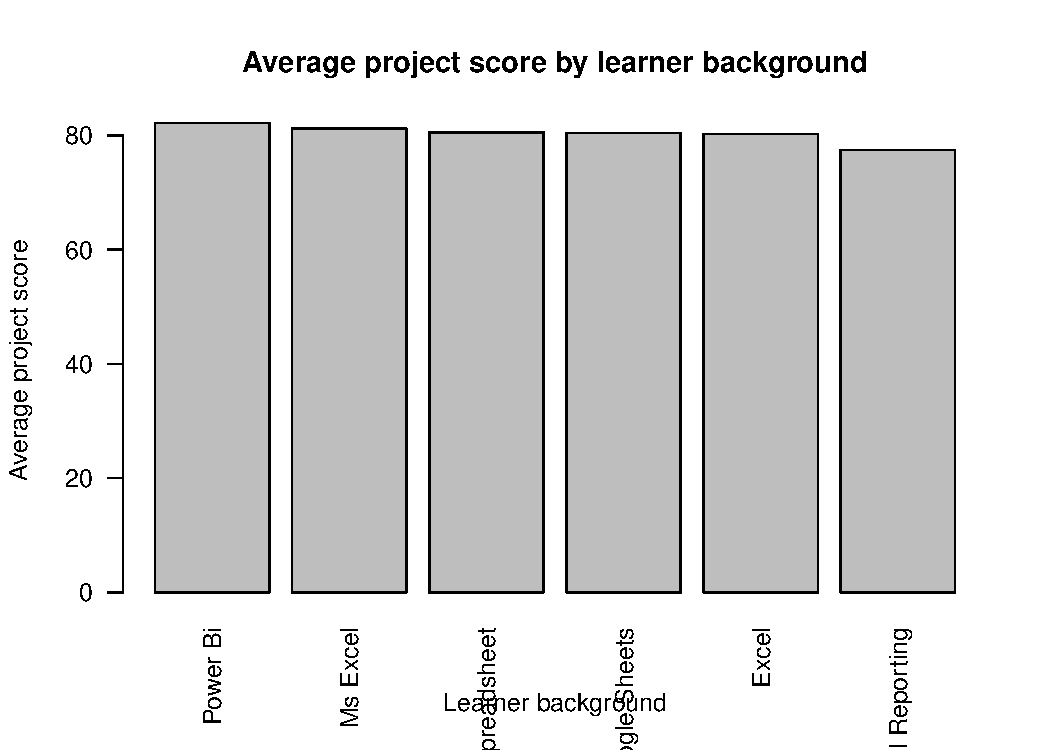
\includegraphics[width=0.9\linewidth,height=\textheight,keepaspectratio,alt={A bar plot showing average project score by learner background, created with base R graphics.}]{chapters/16-data-visualization_files/figure-pdf/fig-16-1-base-r-barplot-1.pdf}

}

\caption{\label{fig-16-1-base-r-barplot}A Base R Bar Plot of Average
Project Score by Learner Background.}

\end{figure}%

The code in Listing~\ref{lst-fig-16-1-base-r-barplot} produces
Figure~\ref{fig-16-1-base-r-barplot}.

Leo can read the chart. It does the job.

But he also notices the friction. The data frame is not used as a whole
inside \texttt{barplot()}. The bar heights are passed as one vector. The
labels are passed as another vector. The title, x-axis label, and y-axis
label are additional arguments. This is not wrong, but it feels less
connected to the shape of the data frame.

That friction becomes more visible as plots become more complex.

If Leo wants a scatter plot with colour by completion status, a line
plot by learning mode, a faceted comparison by region, and carefully
controlled scales, base R can do many of these things, but the code
often becomes more manual.

So the issue is not whether base R works. It does.

The issue is whether Leo wants a plotting system that scales with the
kind of layered, data-frame-based workflow he has been learning.

\section{Other Visualization Tools Leo May
Encounter}\label{other-visualization-tools-leo-may-encounter}

R has more than one graphics system. That can feel confusing at first,
but it is also a strength. Different tools serve different purposes.

Some are good for quick diagnostic plots. Some are good for multi-panel
statistical graphics. Some are good for interactivity. Some are good for
dashboards or maps. Some are designed around a grammar of graphics.

\begin{codelisting}

\caption{\label{lst-tbl-16-1-visualization-tools}Code for A Practical
Comparison of Common R Visualization Approaches}

\centering{

\begin{Shaded}
\begin{Highlighting}[]
\NormalTok{tibble}\SpecialCharTok{::}\FunctionTok{tribble}\NormalTok{(}
  \SpecialCharTok{\textasciitilde{}}\NormalTok{Approach, }\SpecialCharTok{\textasciitilde{}}\NormalTok{Best\_for, }\SpecialCharTok{\textasciitilde{}}\NormalTok{How\_Leo\_should\_think\_about\_it,}
  \StringTok{"Base R graphics"}\NormalTok{, }\StringTok{"Quick plots, teaching examples, older statistical workflows"}\NormalTok{, }\StringTok{"Useful and always available, but complex designs may require more manual control."}\NormalTok{,}
  \StringTok{"lattice"}\NormalTok{, }\StringTok{"Conditioning plots and multi{-}panel statistical graphics"}\NormalTok{, }\StringTok{"A powerful system Leo may meet in older or specialist R materials."}\NormalTok{,}
  \StringTok{"plotly"}\NormalTok{, }\StringTok{"Interactive charts that users can hover, zoom, and explore"}\NormalTok{, }\StringTok{"Often used to make existing plots interactive, especially with ggplotly()."}\NormalTok{,}
  \StringTok{"Shiny"}\NormalTok{, }\StringTok{"Interactive web applications and dashboards"}\NormalTok{, }\StringTok{"Not just a plotting package. It builds user interfaces around analysis and visuals."}\NormalTok{,}
  \StringTok{"ggplot2"}\NormalTok{, }\StringTok{"Layered, reproducible, grammar{-}based graphics from data frames"}\NormalTok{, }\StringTok{"The main system in this chapter because it fits Leo\textquotesingle{}s tidy data workflow."}
\NormalTok{) }\SpecialCharTok{|\textgreater{}}
\NormalTok{  knitr}\SpecialCharTok{::}\FunctionTok{kable}\NormalTok{()}
\end{Highlighting}
\end{Shaded}

}

\end{codelisting}%

{

\begin{longtable}[]{@{}
  >{\raggedright\arraybackslash}p{(\linewidth - 4\tabcolsep) * \real{0.0982}}
  >{\raggedright\arraybackslash}p{(\linewidth - 4\tabcolsep) * \real{0.3865}}
  >{\raggedright\arraybackslash}p{(\linewidth - 4\tabcolsep) * \real{0.5153}}@{}}

\caption{\label{tbl-16-1-visualization-tools}A Practical Comparison of
Common R Visualization Approaches.}

\tabularnewline

\toprule\noalign{}
\begin{minipage}[b]{\linewidth}\raggedright
Approach
\end{minipage} & \begin{minipage}[b]{\linewidth}\raggedright
Best\_for
\end{minipage} & \begin{minipage}[b]{\linewidth}\raggedright
How\_Leo\_should\_think\_about\_it
\end{minipage} \\
\midrule\noalign{}
\endhead
\bottomrule\noalign{}
\endlastfoot
Base R graphics & Quick plots, teaching examples, older statistical
workflows & Useful and always available, but complex designs may require
more manual control. \\
lattice & Conditioning plots and multi-panel statistical graphics & A
powerful system Leo may meet in older or specialist R materials. \\
plotly & Interactive charts that users can hover, zoom, and explore &
Often used to make existing plots interactive, especially with
ggplotly(). \\
Shiny & Interactive web applications and dashboards & Not just a
plotting package. It builds user interfaces around analysis and
visuals. \\
ggplot2 & Layered, reproducible, grammar-based graphics from data frames
& The main system in this chapter because it fits Leo's tidy data
workflow. \\

\end{longtable}

}

The code in Listing~\ref{lst-tbl-16-1-visualization-tools} creates
Table~\ref{tbl-16-1-visualization-tools}.

This chapter will focus on \texttt{ggplot2}, but that does not mean the
other systems are inferior. A professional R user learns to recognise
the purpose of each tool.

\texttt{lattice}, developed around trellis graphics, remains important
in some statistical contexts and older R books (Sarkar, 2008).
\texttt{plotly} can turn plots into interactive web graphics, and it is
especially useful when the reader needs to explore details rather than
only view a printed figure (Sievert, 2020). Shiny is a framework for
building interactive R applications, not merely a plot function. It
becomes important when analysis needs controls, filters, user inputs, or
dashboards.

For Leo's current stage, however, \texttt{ggplot2} is the right centre
of gravity. It connects naturally to data frames, tidy data, pipes,
grouping, summaries, and reproducible code.

\section{The Grammar of Graphics: The Idea Behind
ggplot2}\label{the-grammar-of-graphics-the-idea-behind-ggplot2}

The name \texttt{ggplot2} comes from the grammar of graphics, a way of
thinking about statistical graphics associated with Wilkinson (2005) and
implemented for R by Wickham (2016).

A grammar matters because it gives Leo something deeper than a catalogue
of chart types.

Instead of memorising one command for scatter plots, another for bar
charts, another for lines, and another for histograms, Leo learns the
building blocks behind them.

A plot is built from parts:

\begin{itemize}
\tightlist
\item
  \textbf{data} supplies the evidence
\item
  \textbf{aesthetic mappings} connect variables to visual attributes
\item
  \textbf{geometries} choose the visual marks, such as points, lines, or
  bars
\item
  \textbf{statistical transformations} compute counts, bins, means, or
  summaries when needed
\item
  \textbf{scales} translate data values into positions, colours, sizes,
  and labels
\item
  \textbf{facets} split one plot into small panels
\item
  \textbf{themes} control non-data appearance
\item
  \textbf{coordinates} control the plotting space
\item
  \textbf{layers} are drawn in order
\end{itemize}

This is the lightbulb moment.

Leo is not asking R to ``make a chart'' in one mysterious act. He is
building a visual argument from understandable parts.

The most basic mental model is:

\begin{codelisting}

\caption{\label{lst-chapter16-ggplot-template}Code for the Basic ggplot2
Template}

\centering{

\begin{Shaded}
\begin{Highlighting}[]
\FunctionTok{ggplot}\NormalTok{(}\AttributeTok{data =}\NormalTok{ ...) }\SpecialCharTok{+}
  \FunctionTok{geom\_...}\NormalTok{(}\AttributeTok{mapping =} \FunctionTok{aes}\NormalTok{(...))}
\end{Highlighting}
\end{Shaded}

}

\end{codelisting}%

The code in Listing~\ref{lst-chapter16-ggplot-template} gives Leo the
basic grammar-of-graphics template.

Read that slowly.

\texttt{ggplot(data\ =\ ...)} starts with the data frame.

\texttt{aes(...)} says how variables in that data frame should become
visual properties.

\texttt{geom\_...()} says what kind of mark should be drawn.

The \texttt{+} sign adds parts to the plot.

\begin{tcolorbox}[enhanced jigsaw, arc=.35mm, bottomrule=.15mm, breakable, colback=white, colframe=quarto-callout-important-color-frame, left=2mm, leftrule=.75mm, opacityback=0, rightrule=.15mm, toprule=.15mm]
\begin{minipage}[t]{5.5mm}
\textcolor{quarto-callout-important-color}{\faExclamation}
\end{minipage}%
\begin{minipage}[t]{\textwidth - 5.5mm}

\vspace{-3mm}\textbf{The ggplot2 sentence}\vspace{3mm}

A \texttt{ggplot2} plot reads like a sentence: ``Use this data, map
these variables, draw this kind of mark, then add more instructions if
needed.''

\end{minipage}%
\end{tcolorbox}

\section{The First ggplot2 Plot: Study Hours and Project
Score}\label{the-first-ggplot2-plot-study-hours-and-project-score}

Leo begins with a question that fits a scatter plot:

\begin{quote}
Do learners who study more hours tend to have higher project scores?
\end{quote}

A scatter plot is useful when both variables are numeric and Leo wants
to see the relationship between them.

\begin{codelisting}

\caption{\label{lst-fig-16-2-scatter-study-hours-project-score}Code for
Study Hours and Project Score Shown as a ggplot2 Scatter Plot}

\centering{

\begin{Shaded}
\begin{Highlighting}[]
\FunctionTok{ggplot}\NormalTok{(}
  \AttributeTok{data =}\NormalTok{ df\_plot,}
  \AttributeTok{mapping =} \FunctionTok{aes}\NormalTok{(}\AttributeTok{x =}\NormalTok{ study\_hours, }\AttributeTok{y =}\NormalTok{ project\_score)}
\NormalTok{) }\SpecialCharTok{+}
  \FunctionTok{geom\_point}\NormalTok{(}\AttributeTok{alpha =} \FloatTok{0.65}\NormalTok{) }\SpecialCharTok{+}
  \FunctionTok{labs}\NormalTok{(}
    \AttributeTok{title =} \StringTok{"Study hours and project score"}\NormalTok{,}
    \AttributeTok{x =} \StringTok{"Study hours"}\NormalTok{,}
    \AttributeTok{y =} \StringTok{"Project score"}
\NormalTok{  ) }\SpecialCharTok{+}
  \FunctionTok{theme\_minimal}\NormalTok{()}
\end{Highlighting}
\end{Shaded}

}

\end{codelisting}%

\begin{figure}[H]

\centering{

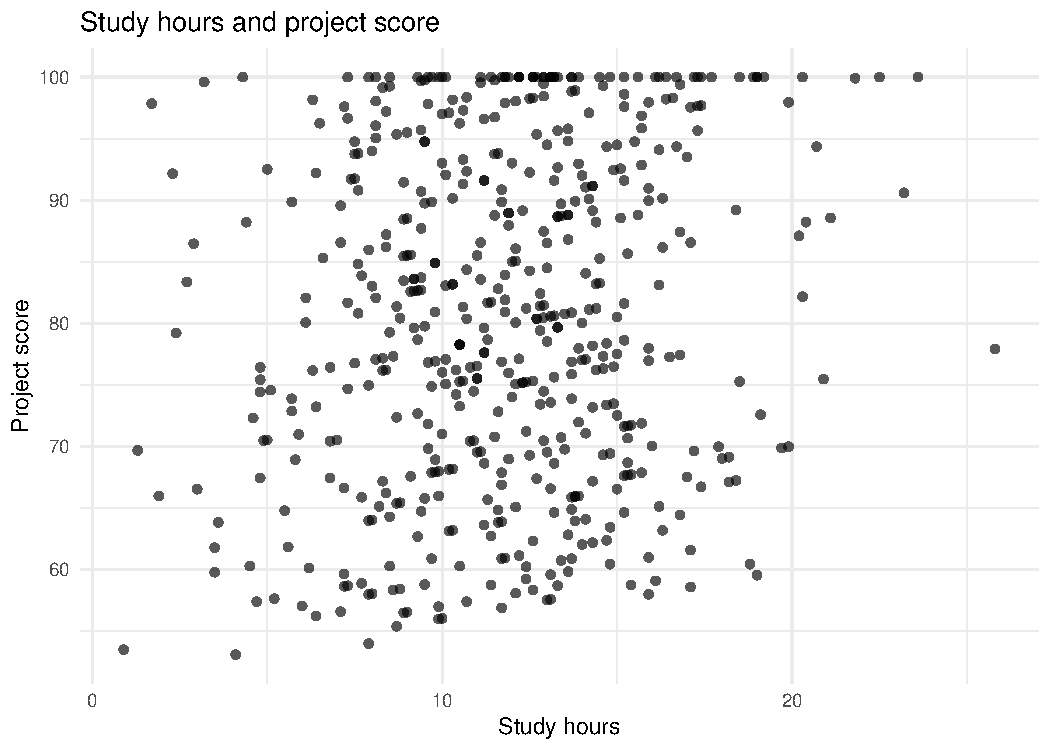
\includegraphics[width=0.9\linewidth,height=\textheight,keepaspectratio,alt={A scatter plot showing weekly study hours on the x-axis and project score on the y-axis.}]{chapters/16-data-visualization_files/figure-pdf/fig-16-2-scatter-study-hours-project-score-1.pdf}

}

\caption{\label{fig-16-2-scatter-study-hours-project-score}Study Hours
and Project Score Shown as a ggplot2 Scatter Plot.}

\end{figure}%

The code in Listing~\ref{lst-fig-16-2-scatter-study-hours-project-score}
produces Figure~\ref{fig-16-2-scatter-study-hours-project-score}.

The code in Listing~\ref{lst-fig-16-2-scatter-study-hours-project-score}
has three main parts.

First, \texttt{data\ =\ df\_plot} supplies the evidence.

Second, \texttt{aes(x\ =\ study\_hours,\ y\ =\ project\_score)} maps
variables to axes. The variable \texttt{study\_hours} becomes horizontal
position. The variable \texttt{project\_score} becomes vertical
position.

Third, \texttt{geom\_point()} draws one point for each row.

The plot does not prove a cause. It does not say that study hours alone
determine project score. But it lets Leo see the relationship as a
pattern rather than a column of numbers.

He can now ask better questions.

Are the points generally rising? Are there learners with many study
hours but low project scores? Are there learners with high scores
despite fewer hours? Does the relationship differ by background or
learning mode?

Visualization does not end analysis. It sharpens analysis.

\section{Aesthetic Mappings with
aes()}\label{aesthetic-mappings-with-aes}

The function \texttt{aes()} is one of the most important ideas in this
chapter.

It tells \texttt{ggplot2} how variables in the data should become
visible parts of the plot.

Common aesthetics include:

\begin{itemize}
\tightlist
\item
  \texttt{x}
\item
  \texttt{y}
\item
  \texttt{color}
\item
  \texttt{fill}
\item
  \texttt{size}
\item
  \texttt{shape}
\item
  \texttt{group}
\item
  \texttt{alpha}
\end{itemize}

For example:

\begin{codelisting}

\caption{\label{lst-chapter16-aes-color-example}Code for Mapping
Completion Status to Colour}

\centering{

\begin{Shaded}
\begin{Highlighting}[]
\FunctionTok{ggplot}\NormalTok{(df\_plot, }\FunctionTok{aes}\NormalTok{(}\AttributeTok{x =}\NormalTok{ study\_hours, }\AttributeTok{y =}\NormalTok{ project\_score, }\AttributeTok{color =}\NormalTok{ completion\_status)) }\SpecialCharTok{+}
  \FunctionTok{geom\_point}\NormalTok{()}
\end{Highlighting}
\end{Shaded}

}

\end{codelisting}%

\begin{figure}[H]

\centering{

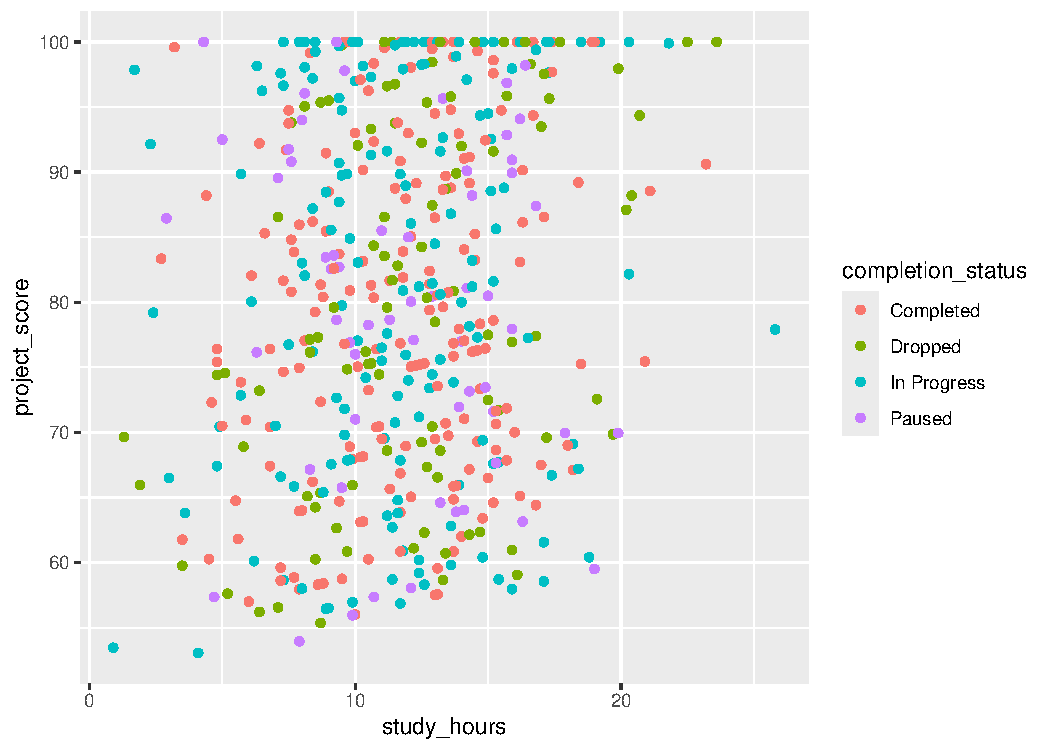
\includegraphics[width=0.9\linewidth,height=\textheight,keepaspectratio,alt={A scatter plot of weekly study hours and project score, with point colour mapped to completion status.}]{chapters/16-data-visualization_files/figure-pdf/fig-16-aes-color-example-1.pdf}

}

\caption{\label{fig-16-aes-color-example}Mapping Completion Status to
Colour in a Scatter Plot}

\end{figure}%

The code in Listing~\ref{lst-chapter16-aes-color-example} produces
Figure~\ref{fig-16-aes-color-example} and means:

\begin{quote}
Put \texttt{study\_hours} on the x-axis, put \texttt{project\_score} on
the y-axis, and use different colours for different values of
\texttt{completion\_status}.
\end{quote}

The important phrase is ``different values.'' When Leo writes a variable
inside \texttt{aes()}, he is mapping the values of that variable to a
visual property.

That is different from setting a property to a fixed value.

\section{Mapping Versus Setting}\label{mapping-versus-setting}

One of the most common beginner mistakes in \texttt{ggplot2} is
confusing mapping with setting.

Mapping connects a variable to a visual attribute.

Setting gives a visual attribute one fixed value.

These two lines look similar, but they mean very different things:

\begin{codelisting}

\caption{\label{lst-chapter16-mapping-setting}Code for Comparing Mapping
and Setting}

\centering{

\begin{Shaded}
\begin{Highlighting}[]
\FunctionTok{aes}\NormalTok{(}\AttributeTok{color =}\NormalTok{ completion\_status)}

\NormalTok{color }\OtherTok{=} \StringTok{"steelblue"}
\end{Highlighting}
\end{Shaded}

}

\end{codelisting}%

The code in Listing~\ref{lst-chapter16-mapping-setting} contrasts
mapping and setting.

The first line maps a variable. It tells \texttt{ggplot2} to use colour
to represent different completion statuses.

The second line sets a constant. It tells \texttt{ggplot2} to make the
points steelblue, regardless of what the data say.

Leo can see the difference in code.

\begin{codelisting}

\caption{\label{lst-fig-16-3-mapping-completion-status}Code for Mapping
Completion Status to Colour in a Scatter Plot}

\centering{

\begin{Shaded}
\begin{Highlighting}[]
\FunctionTok{ggplot}\NormalTok{(}
  \AttributeTok{data =}\NormalTok{ df\_plot,}
  \AttributeTok{mapping =} \FunctionTok{aes}\NormalTok{(}\AttributeTok{x =}\NormalTok{ study\_hours, }\AttributeTok{y =}\NormalTok{ project\_score, }\AttributeTok{color =}\NormalTok{ completion\_status)}
\NormalTok{) }\SpecialCharTok{+}
  \FunctionTok{geom\_point}\NormalTok{(}\AttributeTok{alpha =} \FloatTok{0.65}\NormalTok{) }\SpecialCharTok{+}
  \FunctionTok{labs}\NormalTok{(}
    \AttributeTok{title =} \StringTok{"Study hours and project score by completion status"}\NormalTok{,}
    \AttributeTok{x =} \StringTok{"Study hours"}\NormalTok{,}
    \AttributeTok{y =} \StringTok{"Project score"}\NormalTok{,}
    \AttributeTok{color =} \StringTok{"Completion status"}
\NormalTok{  ) }\SpecialCharTok{+}
  \FunctionTok{theme\_minimal}\NormalTok{()}
\end{Highlighting}
\end{Shaded}

}

\end{codelisting}%

\begin{figure}[H]

\centering{

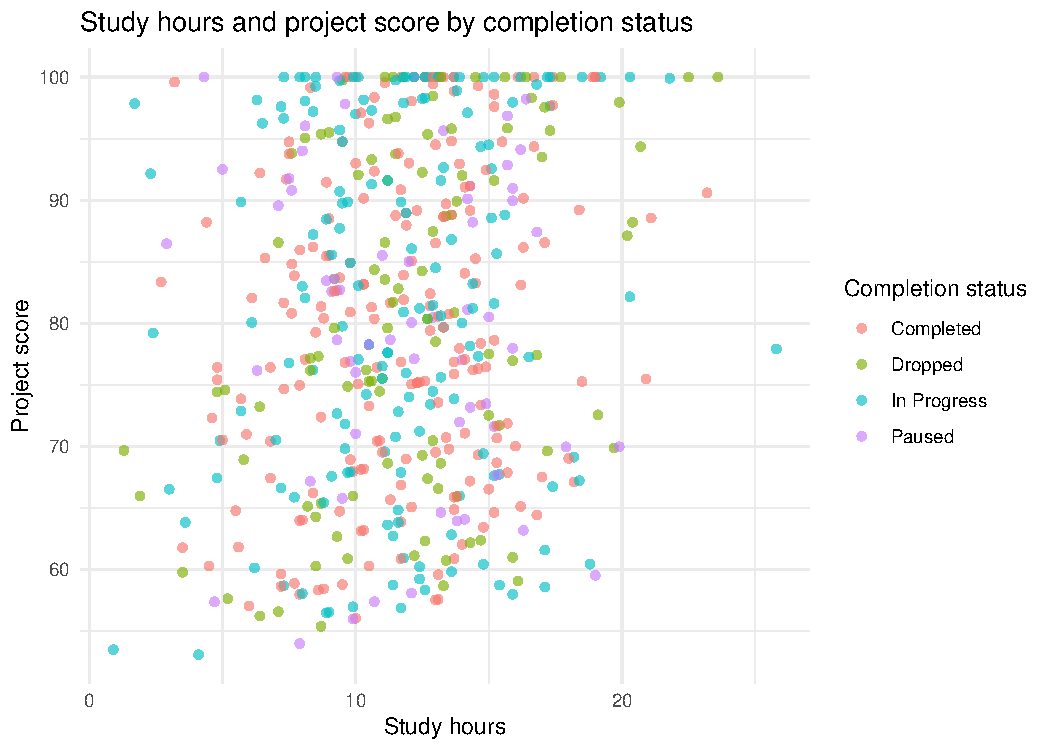
\includegraphics[width=0.9\linewidth,height=\textheight,keepaspectratio,alt={A scatter plot of study hours and project score, with points coloured by learner completion status.}]{chapters/16-data-visualization_files/figure-pdf/fig-16-3-mapping-completion-status-1.pdf}

}

\caption{\label{fig-16-3-mapping-completion-status}Mapping Completion
Status to Colour in a Scatter Plot.}

\end{figure}%

The code in Listing~\ref{lst-fig-16-3-mapping-completion-status}
produces Figure~\ref{fig-16-3-mapping-completion-status}.

Here, colour carries information. It helps Leo see whether the
relationship between study hours and project score differs across
completion groups.

Now compare that with a fixed colour:

\begin{codelisting}

\caption{\label{lst-chapter16-fixed-color-example}Code for Setting One
Fixed Point Colour}

\centering{

\begin{Shaded}
\begin{Highlighting}[]
\FunctionTok{ggplot}\NormalTok{(}
  \AttributeTok{data =}\NormalTok{ df\_plot,}
  \AttributeTok{mapping =} \FunctionTok{aes}\NormalTok{(}\AttributeTok{x =}\NormalTok{ study\_hours, }\AttributeTok{y =}\NormalTok{ project\_score)}
\NormalTok{) }\SpecialCharTok{+}
  \FunctionTok{geom\_point}\NormalTok{(}\AttributeTok{color =} \StringTok{"steelblue"}\NormalTok{)}
\end{Highlighting}
\end{Shaded}

}

\end{codelisting}%

\begin{figure}[H]

\centering{

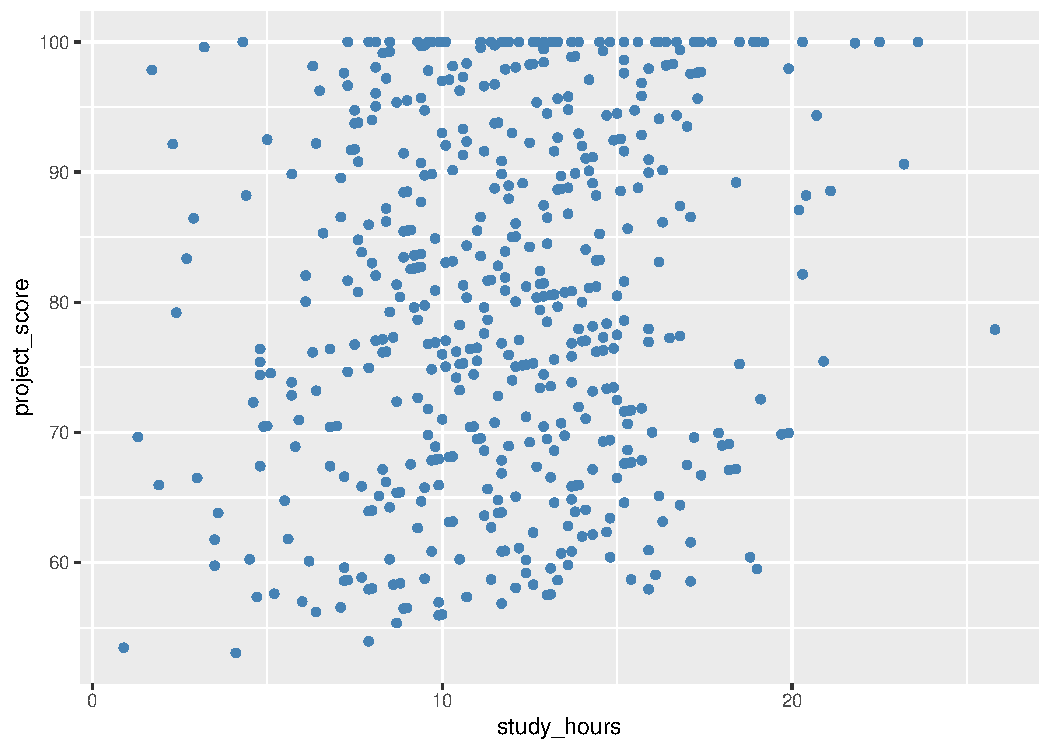
\includegraphics[width=0.9\linewidth,height=\textheight,keepaspectratio,alt={A scatter plot of study hours and project score, with all points shown in one fixed colour.}]{chapters/16-data-visualization_files/figure-pdf/fig-16-fixed-colour-example-1.pdf}

}

\caption{\label{fig-16-fixed-colour-example}Setting One Fixed Colour for
All Points}

\end{figure}%

The code in Listing~\ref{lst-chapter16-fixed-color-example} produces
Figure~\ref{fig-16-fixed-colour-example}.

In the second version, colour does not carry information. It only
controls appearance.

\begin{tcolorbox}[enhanced jigsaw, arc=.35mm, bottomrule=.15mm, breakable, colback=white, colframe=quarto-callout-tip-color-frame, left=2mm, leftrule=.75mm, opacityback=0, rightrule=.15mm, toprule=.15mm]
\begin{minipage}[t]{5.5mm}
\textcolor{quarto-callout-tip-color}{\faLightbulb}
\end{minipage}%
\begin{minipage}[t]{\textwidth - 5.5mm}

\vspace{-3mm}\textbf{The mapping test}\vspace{3mm}

If the visual property should change according to a variable in the
data, put it inside \texttt{aes()}. If the visual property should stay
the same for every mark, put it outside \texttt{aes()}.

\end{minipage}%
\end{tcolorbox}

This small distinction prevents many confusing plots.

\section{Geometric Layers: The Marks on the
Page}\label{geometric-layers-the-marks-on-the-page}

The \texttt{geom\_*()} function decides what kind of visual mark
appears.

A point, a line, and a bar are not just different decorations. They
answer different kinds of questions.

\begin{codelisting}

\caption{\label{lst-tbl-16-2-common-geoms}Code for Common ggplot2 Geoms
and When Leo Should Use Them}

\centering{

\begin{Shaded}
\begin{Highlighting}[]
\NormalTok{tibble}\SpecialCharTok{::}\FunctionTok{tribble}\NormalTok{(}
  \SpecialCharTok{\textasciitilde{}}\NormalTok{Geom, }\SpecialCharTok{\textasciitilde{}}\NormalTok{Common\_use, }\SpecialCharTok{\textasciitilde{}}\NormalTok{Typical\_question,}
  \StringTok{"\textasciigrave{}geom\_point()\textasciigrave{}"}\NormalTok{, }\StringTok{"Scatter plots for two numeric variables"}\NormalTok{, }\StringTok{"How are two numeric variables related?"}\NormalTok{,}
  \StringTok{"\textasciigrave{}geom\_line()\textasciigrave{}"}\NormalTok{, }\StringTok{"Trends across an ordered variable such as time or week"}\NormalTok{, }\StringTok{"How does a value change across an ordered sequence?"}\NormalTok{,}
  \StringTok{"\textasciigrave{}geom\_bar()\textasciigrave{}"}\NormalTok{, }\StringTok{"Counts of observations in categories"}\NormalTok{, }\StringTok{"How many rows fall into each category?"}\NormalTok{,}
  \StringTok{"\textasciigrave{}geom\_col()\textasciigrave{}"}\NormalTok{, }\StringTok{"Bars where the height is already computed"}\NormalTok{, }\StringTok{"How large is a prepared summary value for each category?"}\NormalTok{,}
  \StringTok{"\textasciigrave{}geom\_histogram()\textasciigrave{}"}\NormalTok{, }\StringTok{"Distribution of one numeric variable using bins"}\NormalTok{, }\StringTok{"How are values spread across ranges?"}\NormalTok{,}
  \StringTok{"\textasciigrave{}geom\_boxplot()\textasciigrave{}"}\NormalTok{, }\StringTok{"Distribution of a numeric variable across groups"}\NormalTok{, }\StringTok{"How do distributions compare across categories?"}
\NormalTok{) }\SpecialCharTok{|\textgreater{}}
\NormalTok{  knitr}\SpecialCharTok{::}\FunctionTok{kable}\NormalTok{()}
\end{Highlighting}
\end{Shaded}

}

\end{codelisting}%

{

\begin{longtable}[]{@{}
  >{\raggedright\arraybackslash}p{(\linewidth - 4\tabcolsep) * \real{0.1450}}
  >{\raggedright\arraybackslash}p{(\linewidth - 4\tabcolsep) * \real{0.4198}}
  >{\raggedright\arraybackslash}p{(\linewidth - 4\tabcolsep) * \real{0.4351}}@{}}

\caption{\label{tbl-16-2-common-geoms}Common ggplot2 Geoms and When Leo
Should Use Them.}

\tabularnewline

\toprule\noalign{}
\begin{minipage}[b]{\linewidth}\raggedright
Geom
\end{minipage} & \begin{minipage}[b]{\linewidth}\raggedright
Common\_use
\end{minipage} & \begin{minipage}[b]{\linewidth}\raggedright
Typical\_question
\end{minipage} \\
\midrule\noalign{}
\endhead
\bottomrule\noalign{}
\endlastfoot
\texttt{geom\_point()} & Scatter plots for two numeric variables & How
are two numeric variables related? \\
\texttt{geom\_line()} & Trends across an ordered variable such as time
or week & How does a value change across an ordered sequence? \\
\texttt{geom\_bar()} & Counts of observations in categories & How many
rows fall into each category? \\
\texttt{geom\_col()} & Bars where the height is already computed & How
large is a prepared summary value for each category? \\
\texttt{geom\_histogram()} & Distribution of one numeric variable using
bins & How are values spread across ranges? \\
\texttt{geom\_boxplot()} & Distribution of a numeric variable across
groups & How do distributions compare across categories? \\

\end{longtable}

}

The code in Listing~\ref{lst-tbl-16-2-common-geoms} creates
Table~\ref{tbl-16-2-common-geoms}.

The table is not a list to memorise. It is a decision aid.

Leo should begin with the question:

\begin{quote}
What kind of comparison am I trying to make visible?
\end{quote}

Then he chooses the geom.

\section{Bar Charts: Counts and Prepared
Values}\label{bar-charts-counts-and-prepared-values}

Bar charts create frequent confusion because \texttt{ggplot2} has both
\texttt{geom\_bar()} and \texttt{geom\_col()}.

They look similar, but they do different jobs.

\texttt{geom\_bar()} counts rows.

\begin{codelisting}

\caption{\label{lst-fig-16-4-geom-bar-completion-count}Code for
Completion Status Counted Directly with Geom\_bar()}

\centering{

\begin{Shaded}
\begin{Highlighting}[]
\FunctionTok{ggplot}\NormalTok{(}
  \AttributeTok{data =}\NormalTok{ df\_plot,}
  \AttributeTok{mapping =} \FunctionTok{aes}\NormalTok{(}\AttributeTok{x =}\NormalTok{ completion\_status)}
\NormalTok{) }\SpecialCharTok{+}
  \FunctionTok{geom\_bar}\NormalTok{() }\SpecialCharTok{+}
  \FunctionTok{labs}\NormalTok{(}
    \AttributeTok{title =} \StringTok{"Number of learners by completion status"}\NormalTok{,}
    \AttributeTok{x =} \StringTok{"Completion status"}\NormalTok{,}
    \AttributeTok{y =} \StringTok{"Number of learners"}
\NormalTok{  ) }\SpecialCharTok{+}
  \FunctionTok{theme\_minimal}\NormalTok{()}
\end{Highlighting}
\end{Shaded}

}

\end{codelisting}%

\begin{figure}[H]

\centering{

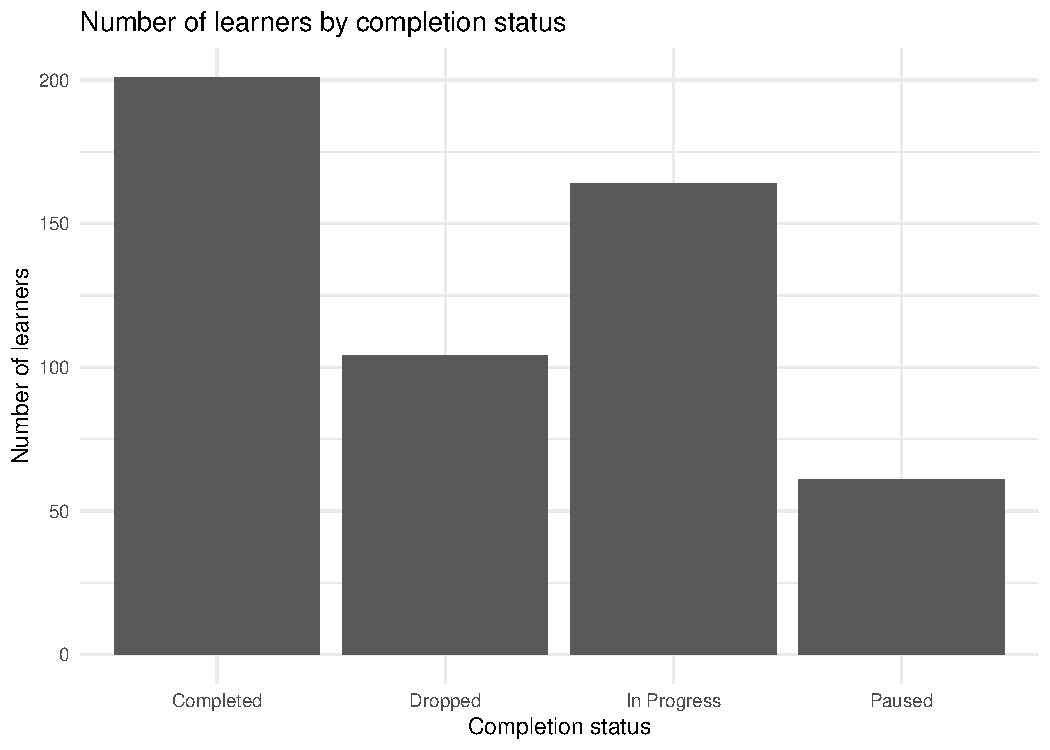
\includegraphics[width=0.9\linewidth,height=\textheight,keepaspectratio,alt={A bar chart showing the number of learners in each completion-status category.}]{chapters/16-data-visualization_files/figure-pdf/fig-16-4-geom-bar-completion-count-1.pdf}

}

\caption{\label{fig-16-4-geom-bar-completion-count}Completion Status
Counted Directly with geom\_bar().}

\end{figure}%

The code in Listing~\ref{lst-fig-16-4-geom-bar-completion-count}
produces Figure~\ref{fig-16-4-geom-bar-completion-count}.

Here, Leo does not calculate the counts first. \texttt{geom\_bar()}
performs a statistical transformation behind the scenes. It counts how
many rows fall into each value of \texttt{completion\_status}.

\texttt{geom\_col()} is different. It expects the bar height to already
exist in the data.

\begin{codelisting}

\caption{\label{lst-chapter16-geom-col-summary}Code for Preparing Values
for geom\_col()}

\centering{

\begin{Shaded}
\begin{Highlighting}[]
\NormalTok{df\_background\_score }\OtherTok{\textless{}{-}}\NormalTok{ df\_plot }\SpecialCharTok{|\textgreater{}}
  \FunctionTok{group\_by}\NormalTok{(background) }\SpecialCharTok{|\textgreater{}}
  \FunctionTok{summarise}\NormalTok{(}
    \AttributeTok{avg\_project\_score =} \FunctionTok{mean}\NormalTok{(project\_score, }\AttributeTok{na.rm =} \ConstantTok{TRUE}\NormalTok{),}
    \AttributeTok{learners =} \FunctionTok{n}\NormalTok{(),}
    \AttributeTok{.groups =} \StringTok{"drop"}
\NormalTok{  ) }\SpecialCharTok{|\textgreater{}}
  \FunctionTok{arrange}\NormalTok{(}\FunctionTok{desc}\NormalTok{(avg\_project\_score))}

\NormalTok{knitr}\SpecialCharTok{::}\FunctionTok{kable}\NormalTok{(df\_background\_score)}
\end{Highlighting}
\end{Shaded}

}

\end{codelisting}%

{

\begin{longtable}[]{@{}lrr@{}}

\caption{\label{tbl-16-background-score-summary}Average Project Score by
Learner Background Prepared for geom\_col().}

\tabularnewline

\toprule\noalign{}
background & avg\_project\_score & learners \\
\midrule\noalign{}
\endhead
\bottomrule\noalign{}
\endlastfoot
Power Bi & 82.14947 & 95 \\
Ms Excel & 81.17623 & 61 \\
Spreadsheet & 80.47098 & 143 \\
Google Sheets & 80.42000 & 90 \\
Excel & 80.25495 & 91 \\
Manual Reporting & 77.41900 & 50 \\

\end{longtable}

}

The code in Listing~\ref{lst-chapter16-geom-col-summary} creates
Table~\ref{tbl-16-background-score-summary}. The code in
Listing~\ref{lst-fig-16-5-geom-col-background-score} uses that prepared
summary to produce Figure~\ref{fig-16-5-geom-col-background-score}.

\begin{codelisting}

\caption{\label{lst-fig-16-5-geom-col-background-score}Code for Average
Project Score by Learner Background Using Geom\_col()}

\centering{

\begin{Shaded}
\begin{Highlighting}[]
\FunctionTok{ggplot}\NormalTok{(}
  \AttributeTok{data =}\NormalTok{ df\_background\_score,}
  \AttributeTok{mapping =} \FunctionTok{aes}\NormalTok{(}\AttributeTok{x =}\NormalTok{ background, }\AttributeTok{y =}\NormalTok{ avg\_project\_score)}
\NormalTok{) }\SpecialCharTok{+}
  \FunctionTok{geom\_col}\NormalTok{() }\SpecialCharTok{+}
  \FunctionTok{labs}\NormalTok{(}
    \AttributeTok{title =} \StringTok{"Average project score by learner background"}\NormalTok{,}
    \AttributeTok{x =} \StringTok{"Learner background"}\NormalTok{,}
    \AttributeTok{y =} \StringTok{"Average project score"}
\NormalTok{  ) }\SpecialCharTok{+}
  \FunctionTok{theme\_minimal}\NormalTok{()}
\end{Highlighting}
\end{Shaded}

}

\end{codelisting}%

\begin{figure}[H]

\centering{

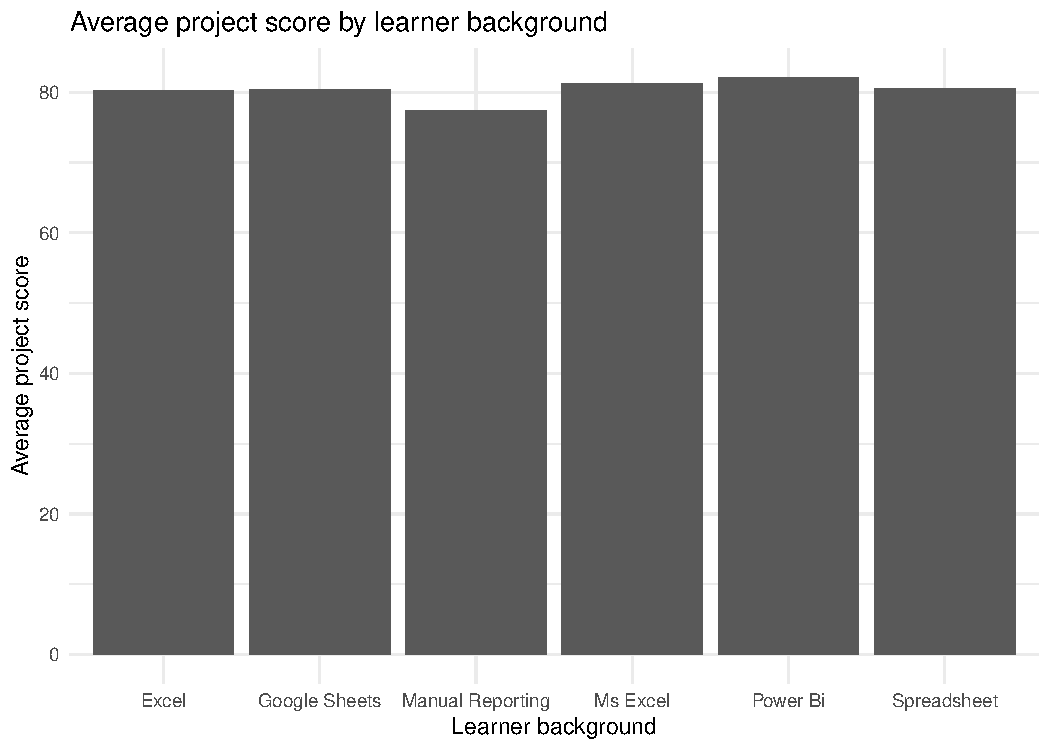
\includegraphics[width=0.9\linewidth,height=\textheight,keepaspectratio,alt={A column chart showing average project score for each learner background category.}]{chapters/16-data-visualization_files/figure-pdf/fig-16-5-geom-col-background-score-1.pdf}

}

\caption{\label{fig-16-5-geom-col-background-score}Average Project Score
by Learner Background Using geom\_col().}

\end{figure}%

In Figure~\ref{fig-16-5-geom-col-background-score}, the average has
already been calculated in \texttt{df\_background\_score}.
\texttt{geom\_col()} simply draws the prepared values.

The difference is worth remembering:

\begin{itemize}
\tightlist
\item
  use \texttt{geom\_bar()} when the plot should count rows
\item
  use \texttt{geom\_col()} when the y-value already exists
\end{itemize}

\section{Histograms: Bins and
Distributions}\label{histograms-bins-and-distributions}

A summary average can hide the shape of a variable.

Suppose Leo calculates the average confidence score. That gives one
number. But one number cannot show whether confidence is clustered,
spread out, skewed, or uneven.

A histogram helps Leo see distribution.

\begin{codelisting}

\caption{\label{lst-fig-16-6-confidence-histogram}Code for Distribution
of Learner Confidence Scores Using Histogram Bins}

\centering{

\begin{Shaded}
\begin{Highlighting}[]
\FunctionTok{ggplot}\NormalTok{(}
  \AttributeTok{data =}\NormalTok{ df\_plot,}
  \AttributeTok{mapping =} \FunctionTok{aes}\NormalTok{(}\AttributeTok{x =}\NormalTok{ confidence\_score)}
\NormalTok{) }\SpecialCharTok{+}
  \FunctionTok{geom\_histogram}\NormalTok{(}\AttributeTok{bins =} \DecValTok{15}\NormalTok{, }\AttributeTok{boundary =} \DecValTok{0}\NormalTok{, }\AttributeTok{closed =} \StringTok{"left"}\NormalTok{) }\SpecialCharTok{+}
  \FunctionTok{labs}\NormalTok{(}
    \AttributeTok{title =} \StringTok{"Distribution of learner confidence scores"}\NormalTok{,}
    \AttributeTok{x =} \StringTok{"Confidence score"}\NormalTok{,}
    \AttributeTok{y =} \StringTok{"Number of learners"}
\NormalTok{  ) }\SpecialCharTok{+}
  \FunctionTok{theme\_minimal}\NormalTok{()}
\end{Highlighting}
\end{Shaded}

}

\end{codelisting}%

\begin{figure}[H]

\centering{

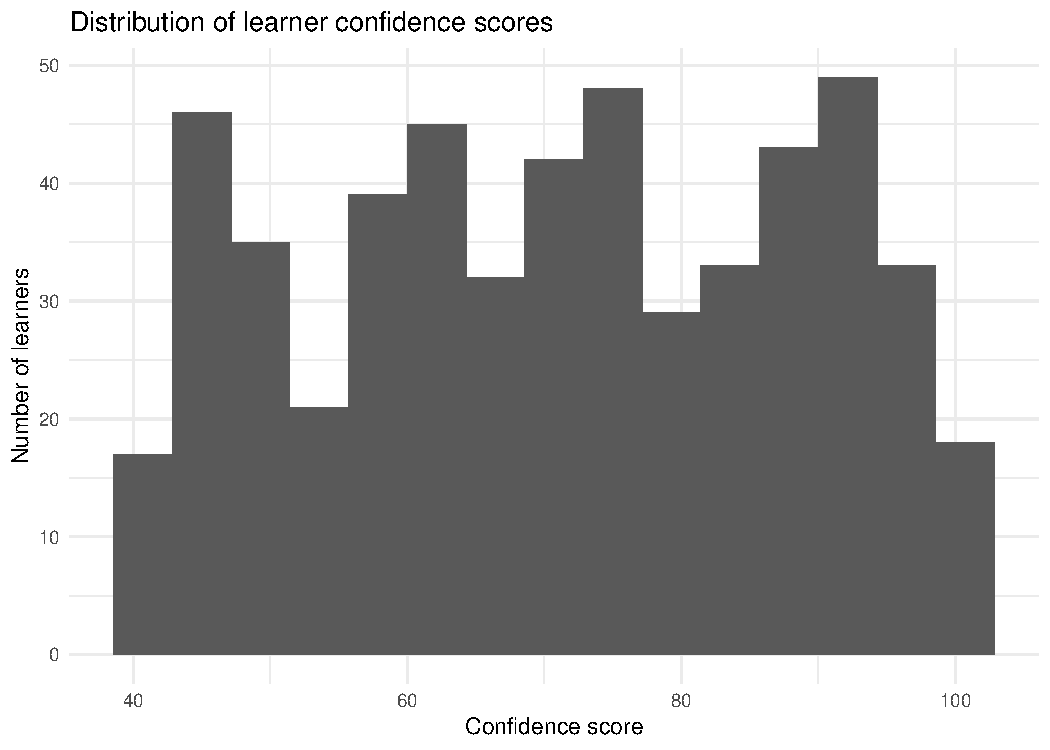
\includegraphics[width=0.9\linewidth,height=\textheight,keepaspectratio,alt={A histogram showing the distribution of learner confidence scores across bins.}]{chapters/16-data-visualization_files/figure-pdf/fig-16-6-confidence-histogram-1.pdf}

}

\caption{\label{fig-16-6-confidence-histogram}Distribution of Learner
Confidence Scores Using Histogram Bins.}

\end{figure}%

The code in Listing~\ref{lst-fig-16-6-confidence-histogram} produces
Figure~\ref{fig-16-6-confidence-histogram}.

The word \texttt{bins} matters. A histogram does not show every value as
a separate category. It divides the numeric range into intervals and
counts how many observations fall into each interval.

This is another statistical transformation. The original data contain
individual confidence scores. The plot calculates counts within bins.

Leo should not treat the number of bins as a purely cosmetic choice. Too
few bins can hide variation. Too many bins can make the pattern noisy.
At this stage, he only needs the habit: check whether the distribution
changes when the binning changes.

\section{Lines: Change Across an Ordered
Variable}\label{lines-change-across-an-ordered-variable}

Line plots are useful when the x-axis has a meaningful order.

\texttt{week} is ordered. Week 2 follows Week 1. Week 3 follows Week 2.
That makes it reasonable to connect values with a line.

Leo first creates a weekly summary.

\begin{codelisting}

\caption{\label{lst-chapter16-weekly-summary}Code for Preparing the
Weekly Project-Score Summary}

\centering{

\begin{Shaded}
\begin{Highlighting}[]
\NormalTok{df\_weekly\_score }\OtherTok{\textless{}{-}}\NormalTok{ df\_plot }\SpecialCharTok{|\textgreater{}}
  \FunctionTok{group\_by}\NormalTok{(week) }\SpecialCharTok{|\textgreater{}}
  \FunctionTok{summarise}\NormalTok{(}
    \AttributeTok{avg\_project\_score =} \FunctionTok{mean}\NormalTok{(project\_score, }\AttributeTok{na.rm =} \ConstantTok{TRUE}\NormalTok{),}
    \AttributeTok{avg\_confidence =} \FunctionTok{mean}\NormalTok{(confidence\_score, }\AttributeTok{na.rm =} \ConstantTok{TRUE}\NormalTok{),}
    \AttributeTok{learners =} \FunctionTok{n}\NormalTok{(),}
    \AttributeTok{.groups =} \StringTok{"drop"}
\NormalTok{  ) }\SpecialCharTok{|\textgreater{}}
  \FunctionTok{arrange}\NormalTok{(week)}

\NormalTok{df\_weekly\_score}
\CommentTok{\#\textgreater{} \# A tibble: 12 x 4}
\CommentTok{\#\textgreater{}     week avg\_project\_score avg\_confidence learners}
\CommentTok{\#\textgreater{}    \textless{}dbl\textgreater{}             \textless{}dbl\textgreater{}          \textless{}dbl\textgreater{}    \textless{}int\textgreater{}}
\CommentTok{\#\textgreater{}  1     1              79.2           68.4       40}
\CommentTok{\#\textgreater{}  2     2              79.3           67.9       38}
\CommentTok{\#\textgreater{}  3     3              82.6           65.4       55}
\CommentTok{\#\textgreater{}  4     4              82.2           70.5       46}
\CommentTok{\#\textgreater{}  5     5              82.6           73.7       46}
\CommentTok{\#\textgreater{}  6     6              77.8           73.2       40}
\CommentTok{\#\textgreater{}  7     7              80.6           73.6       53}
\CommentTok{\#\textgreater{}  8     8              77.7           72.8       36}
\CommentTok{\#\textgreater{}  9     9              82.0           70.4       47}
\CommentTok{\#\textgreater{} 10    10              81.0           72.5       43}
\CommentTok{\#\textgreater{} 11    11              80.5           66.5       41}
\CommentTok{\#\textgreater{} 12    12              79.0           77.2       45}
\end{Highlighting}
\end{Shaded}

}

\end{codelisting}%

The code in Listing~\ref{lst-chapter16-weekly-summary} prepares the
weekly summary used in Figure~\ref{fig-16-7-weekly-line}.

Then he plots the trend.

\begin{codelisting}

\caption{\label{lst-fig-16-7-weekly-line}Code for Average Project Score
Across Weeks}

\centering{

\begin{Shaded}
\begin{Highlighting}[]
\FunctionTok{ggplot}\NormalTok{(}
  \AttributeTok{data =}\NormalTok{ df\_weekly\_score,}
  \AttributeTok{mapping =} \FunctionTok{aes}\NormalTok{(}\AttributeTok{x =}\NormalTok{ week, }\AttributeTok{y =}\NormalTok{ avg\_project\_score)}
\NormalTok{) }\SpecialCharTok{+}
  \FunctionTok{geom\_line}\NormalTok{(}\AttributeTok{linewidth =} \DecValTok{1}\NormalTok{) }\SpecialCharTok{+}
  \FunctionTok{geom\_point}\NormalTok{() }\SpecialCharTok{+}
  \FunctionTok{labs}\NormalTok{(}
    \AttributeTok{title =} \StringTok{"Average project score across weeks"}\NormalTok{,}
    \AttributeTok{x =} \StringTok{"Week"}\NormalTok{,}
    \AttributeTok{y =} \StringTok{"Average project score"}
\NormalTok{  ) }\SpecialCharTok{+}
  \FunctionTok{theme\_minimal}\NormalTok{()}
\end{Highlighting}
\end{Shaded}

}

\end{codelisting}%

\begin{figure}[H]

\centering{

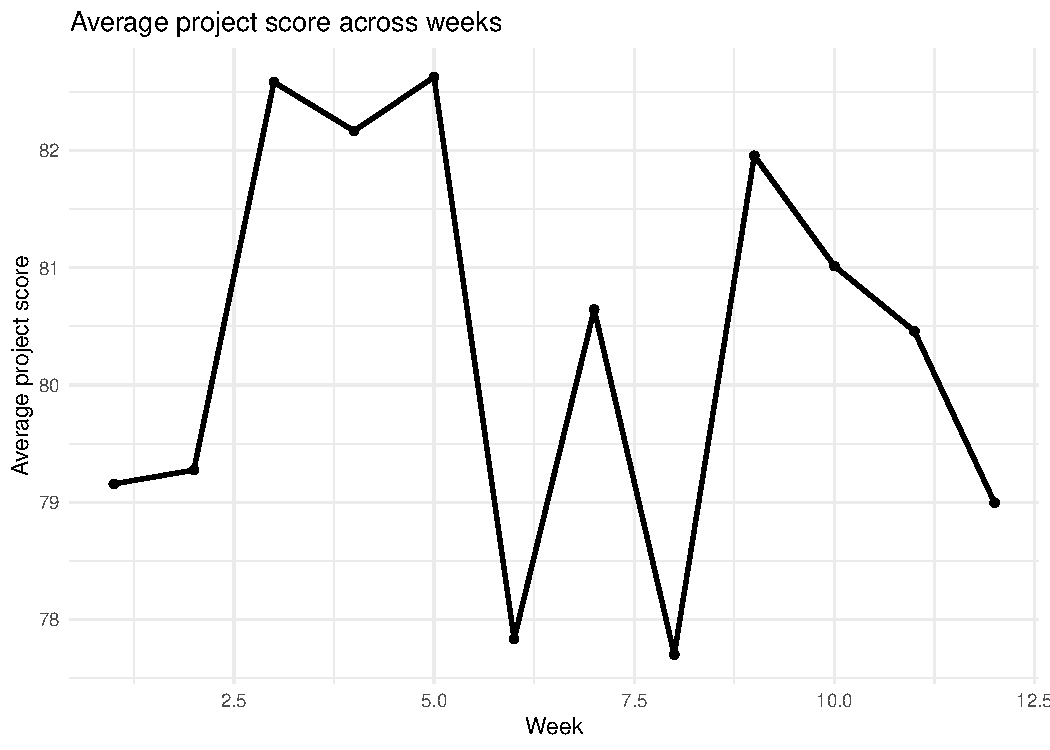
\includegraphics[width=0.9\linewidth,height=\textheight,keepaspectratio,alt={A line chart showing average project score across learning weeks.}]{chapters/16-data-visualization_files/figure-pdf/fig-16-7-weekly-line-1.pdf}

}

\caption{\label{fig-16-7-weekly-line}Average Project Score Across
Weeks.}

\end{figure}%

The code in Listing~\ref{lst-fig-16-7-weekly-line} produces
Figure~\ref{fig-16-7-weekly-line}.

The line works because \texttt{week} has order. It would be a mistake to
connect unordered categories such as country names or backgrounds with a
line. A line implies movement, sequence, or continuity.

That is why Leo should ask:

\begin{quote}
Does the x-axis have a meaningful order?
\end{quote}

If the answer is no, a bar chart, dot plot, or boxplot may be better.

\section{Continuous and Discrete
Variables}\label{continuous-and-discrete-variables}

Plots behave differently depending on the type of variable.

A continuous variable has numeric values across a range. Examples
include \texttt{study\_hours}, \texttt{project\_score},
\texttt{confidence\_score}, \texttt{lessons\_completed}, and
\texttt{payment\_probability\_score}.

A discrete variable has categories. Examples include
\texttt{background}, \texttt{completion\_status},
\texttt{preferred\_learning\_mode}, \texttt{region}, and
\texttt{r\_experience\_level}.

This matters because \texttt{ggplot2} chooses scales based on variable
type.

If Leo maps \texttt{project\_score} to the y-axis, \texttt{ggplot2}
creates a continuous scale. If he maps \texttt{background} to the
x-axis, \texttt{ggplot2} creates a discrete scale. If he maps
\texttt{completion\_status} to colour, \texttt{ggplot2} creates a
discrete colour legend. If he maps \texttt{payment\_probability\_score}
to colour, \texttt{ggplot2} creates a continuous colour scale.

The plot is not only reading names. It is reading types.

That links this chapter back to Chapter 4, where Leo learned that values
have types. Two values can look similar on the screen and still behave
differently inside R. In visualization, that difference becomes visible.

\begin{tcolorbox}[enhanced jigsaw, arc=.35mm, bottomrule=.15mm, breakable, colback=white, colframe=quarto-callout-warning-color-frame, left=2mm, leftrule=.75mm, opacityback=0, rightrule=.15mm, toprule=.15mm]
\begin{minipage}[t]{5.5mm}
\textcolor{quarto-callout-warning-color}{\faExclamationTriangle}
\end{minipage}%
\begin{minipage}[t]{\textwidth - 5.5mm}

\vspace{-3mm}\textbf{Check the type before blaming the plot}\vspace{3mm}

If a numeric variable behaves like categories, it may have been imported
as text. If a category behaves like a numeric scale, it may need to be
converted or recoded. Plotting problems often point back to data type
problems.

\end{minipage}%
\end{tcolorbox}

\section{Grouping: When One Pattern Is Really Several
Patterns}\label{grouping-when-one-pattern-is-really-several-patterns}

Some plots need groups.

In \texttt{ggplot2}, grouping can happen explicitly through
\texttt{group\ =\ ...}, or implicitly through aesthetics such as
\texttt{color}, \texttt{fill}, or \texttt{linetype}.

Leo wants to know whether weekly project scores change differently
across learning modes. He creates a grouped summary.

\begin{codelisting}

\caption{\label{lst-chapter16-weekly-learning-mode-summary}Code for
Preparing Weekly Project Scores by Learning Mode}

\centering{

\begin{Shaded}
\begin{Highlighting}[]
\NormalTok{df\_weekly\_mode }\OtherTok{\textless{}{-}}\NormalTok{ df\_plot }\SpecialCharTok{|\textgreater{}}
  \FunctionTok{group\_by}\NormalTok{(week, preferred\_learning\_mode) }\SpecialCharTok{|\textgreater{}}
  \FunctionTok{summarise}\NormalTok{(}
    \AttributeTok{avg\_project\_score =} \FunctionTok{mean}\NormalTok{(project\_score, }\AttributeTok{na.rm =} \ConstantTok{TRUE}\NormalTok{),}
    \AttributeTok{learners =} \FunctionTok{n}\NormalTok{(),}
    \AttributeTok{.groups =} \StringTok{"drop"}
\NormalTok{  ) }\SpecialCharTok{|\textgreater{}}
  \FunctionTok{arrange}\NormalTok{(preferred\_learning\_mode, week)}

\NormalTok{df\_weekly\_mode}
\CommentTok{\#\textgreater{} \# A tibble: 36 x 4}
\CommentTok{\#\textgreater{}     week preferred\_learning\_mode avg\_project\_score learners}
\CommentTok{\#\textgreater{}    \textless{}dbl\textgreater{} \textless{}chr\textgreater{}                               \textless{}dbl\textgreater{}    \textless{}int\textgreater{}}
\CommentTok{\#\textgreater{}  1     1 Hybrid                               82.2       11}
\CommentTok{\#\textgreater{}  2     2 Hybrid                               75.4       17}
\CommentTok{\#\textgreater{}  3     3 Hybrid                               84.2       21}
\CommentTok{\#\textgreater{}  4     4 Hybrid                               80.9       19}
\CommentTok{\#\textgreater{}  5     5 Hybrid                               85.1       16}
\CommentTok{\#\textgreater{}  6     6 Hybrid                               76.5       13}
\CommentTok{\#\textgreater{}  7     7 Hybrid                               84.3       19}
\CommentTok{\#\textgreater{}  8     8 Hybrid                               72.2        8}
\CommentTok{\#\textgreater{}  9     9 Hybrid                               80.5       16}
\CommentTok{\#\textgreater{} 10    10 Hybrid                               81.9       16}
\CommentTok{\#\textgreater{} \# i 26 more rows}
\end{Highlighting}
\end{Shaded}

}

\end{codelisting}%

The code in Listing~\ref{lst-chapter16-weekly-learning-mode-summary}
prepares the grouped weekly summary used in
Figure~\ref{fig-16-8-grouped-lines-learning-mode}.

Now he maps learning mode to colour and group.

\begin{codelisting}

\caption{\label{lst-fig-16-8-grouped-lines-learning-mode}Code for Weekly
Average Project Score Grouped by Preferred Learning Mode}

\centering{

\begin{Shaded}
\begin{Highlighting}[]
\FunctionTok{ggplot}\NormalTok{(}
  \AttributeTok{data =}\NormalTok{ df\_weekly\_mode,}
  \AttributeTok{mapping =} \FunctionTok{aes}\NormalTok{(}
    \AttributeTok{x =}\NormalTok{ week,}
    \AttributeTok{y =}\NormalTok{ avg\_project\_score,}
    \AttributeTok{color =}\NormalTok{ preferred\_learning\_mode,}
    \AttributeTok{group =}\NormalTok{ preferred\_learning\_mode}
\NormalTok{  )}
\NormalTok{) }\SpecialCharTok{+}
  \FunctionTok{geom\_line}\NormalTok{(}\AttributeTok{linewidth =} \DecValTok{1}\NormalTok{) }\SpecialCharTok{+}
  \FunctionTok{geom\_point}\NormalTok{() }\SpecialCharTok{+}
  \FunctionTok{labs}\NormalTok{(}
    \AttributeTok{title =} \StringTok{"Weekly average project score by learning mode"}\NormalTok{,}
    \AttributeTok{x =} \StringTok{"Week"}\NormalTok{,}
    \AttributeTok{y =} \StringTok{"Average project score"}\NormalTok{,}
    \AttributeTok{color =} \StringTok{"Learning mode"}
\NormalTok{  ) }\SpecialCharTok{+}
  \FunctionTok{theme\_minimal}\NormalTok{()}
\end{Highlighting}
\end{Shaded}

}

\end{codelisting}%

\begin{figure}[H]

\centering{

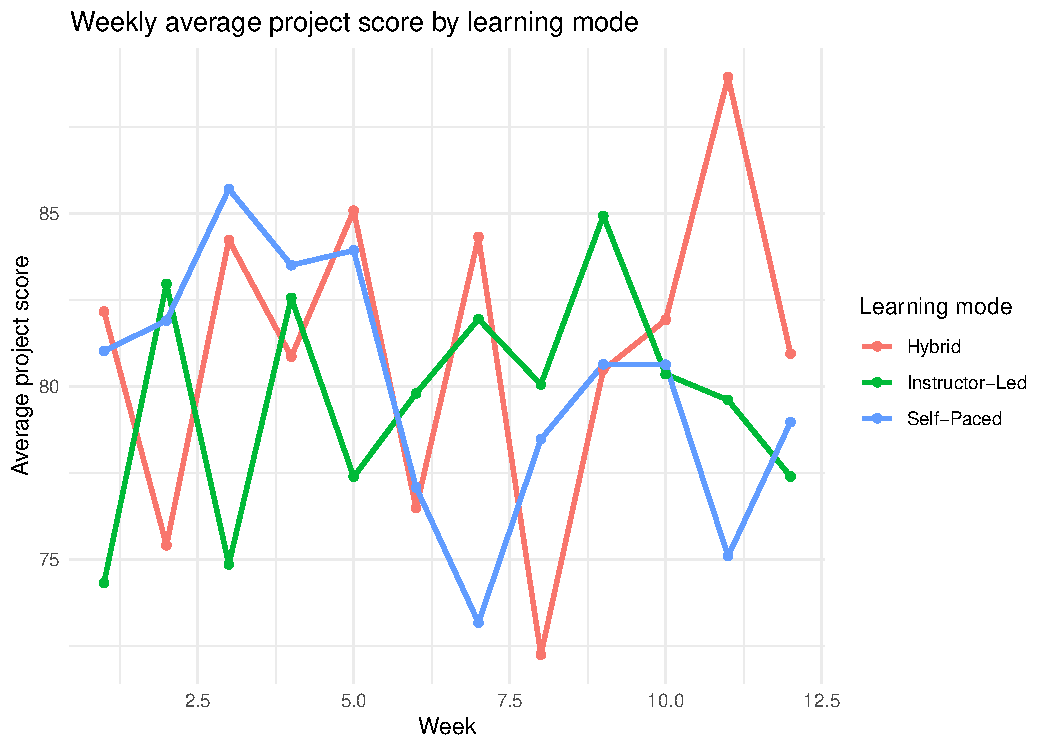
\includegraphics[width=0.9\linewidth,height=\textheight,keepaspectratio,alt={A grouped line chart showing weekly average project score by preferred learning mode.}]{chapters/16-data-visualization_files/figure-pdf/fig-16-8-grouped-lines-learning-mode-1.pdf}

}

\caption{\label{fig-16-8-grouped-lines-learning-mode}Weekly Average
Project Score Grouped by Preferred Learning Mode.}

\end{figure}%

The code in Listing~\ref{lst-fig-16-8-grouped-lines-learning-mode}
produces Figure~\ref{fig-16-8-grouped-lines-learning-mode}.

The \texttt{group} instruction tells \texttt{ggplot2} which points
belong to the same line. In this example, each learning mode gets its
own line.

Colour also separates the groups visually. Without grouping,
\texttt{ggplot2} may connect points in a way that does not match Leo's
question.

The deeper rule is this:

\begin{quote}
When a plot should show several patterns instead of one, Leo must tell R
what defines each pattern.
\end{quote}

\section{Statistical Transformations: Counts, Bins, Means, and
Summaries}\label{statistical-transformations-counts-bins-means-and-summaries}

Some geoms draw the data exactly as supplied. \texttt{geom\_point()}
draws points from existing x and y values.

Other geoms compute something before drawing. \texttt{geom\_bar()}
counts rows. \texttt{geom\_histogram()} bins values and counts
observations in those bins. \texttt{stat\_summary()} can calculate means
or other summaries before drawing.

This is why \texttt{ggplot2} often uses the language of geoms and stats.

Leo does not need advanced statistical graphics yet, but he does need to
know when the plotted value already exists and when the plot is
computing it.

For example, this plot calculates the mean project score inside the
plot:

\begin{codelisting}

\caption{\label{lst-fig-16-9-stat-summary-mean}Code for Mean Project
Score by Preferred Learning Mode Calculated with Stat\_summary()}

\centering{

\begin{Shaded}
\begin{Highlighting}[]
\FunctionTok{ggplot}\NormalTok{(}
  \AttributeTok{data =}\NormalTok{ df\_plot,}
  \AttributeTok{mapping =} \FunctionTok{aes}\NormalTok{(}\AttributeTok{x =}\NormalTok{ preferred\_learning\_mode, }\AttributeTok{y =}\NormalTok{ project\_score)}
\NormalTok{) }\SpecialCharTok{+}
  \FunctionTok{stat\_summary}\NormalTok{(}\AttributeTok{fun =}\NormalTok{ mean, }\AttributeTok{geom =} \StringTok{"point"}\NormalTok{, }\AttributeTok{size =} \DecValTok{3}\NormalTok{) }\SpecialCharTok{+}
  \FunctionTok{stat\_summary}\NormalTok{(}\AttributeTok{fun =}\NormalTok{ mean, }\AttributeTok{geom =} \StringTok{"crossbar"}\NormalTok{, }\AttributeTok{width =} \FloatTok{0.5}\NormalTok{) }\SpecialCharTok{+}
  \FunctionTok{labs}\NormalTok{(}
    \AttributeTok{title =} \StringTok{"Mean project score by preferred learning mode"}\NormalTok{,}
    \AttributeTok{x =} \StringTok{"Preferred learning mode"}\NormalTok{,}
    \AttributeTok{y =} \StringTok{"Mean project score"}
\NormalTok{  ) }\SpecialCharTok{+}
  \FunctionTok{theme\_minimal}\NormalTok{()}
\end{Highlighting}
\end{Shaded}

}

\end{codelisting}%

\begin{figure}[H]

\centering{

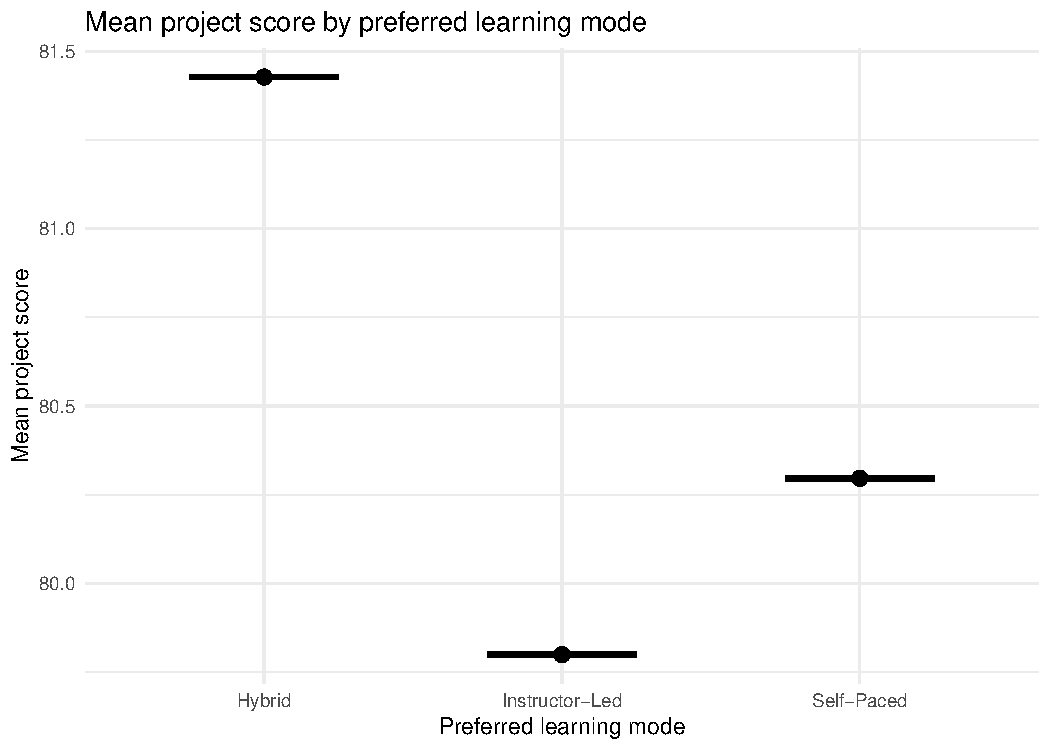
\includegraphics[width=0.9\linewidth,height=\textheight,keepaspectratio,alt={A plot showing mean project score by preferred learning mode using a statistical summary layer.}]{chapters/16-data-visualization_files/figure-pdf/fig-16-9-stat-summary-mean-1.pdf}

}

\caption{\label{fig-16-9-stat-summary-mean}Mean Project Score by
Preferred Learning Mode Calculated with stat\_summary().}

\end{figure}%

The code in Listing~\ref{lst-fig-16-9-stat-summary-mean} produces
Figure~\ref{fig-16-9-stat-summary-mean}.

This is useful for teaching what \texttt{ggplot2} can compute. However,
in serious analysis, Leo should often calculate important summaries
explicitly before plotting. That makes the evidence easier to inspect,
test, and explain.

A good habit is:

\begin{enumerate}
\def\labelenumi{\arabic{enumi}.}
\tightlist
\item
  use plot-level statistics for quick exploration
\item
  create summary tables when the calculation matters to the argument
\item
  plot the inspected summary table when reporting a result
\end{enumerate}

That habit keeps visualization connected to reproducible analysis.

\section{Multi-Layer Rendering Order}\label{multi-layer-rendering-order}

A \texttt{ggplot2} plot is built in layers.

The order matters.

Layers added later are drawn on top of earlier layers. That can help Leo
emphasise important marks, but it can also hide information if he is
careless.

Here is a simple layered plot.

\begin{codelisting}

\caption{\label{lst-fig-16-10-layer-order}Code for A Layered Plot Where
the Summary Mean Is Drawn After the Individual Points}

\centering{

\begin{Shaded}
\begin{Highlighting}[]
\FunctionTok{ggplot}\NormalTok{(}
  \AttributeTok{data =}\NormalTok{ df\_plot,}
  \AttributeTok{mapping =} \FunctionTok{aes}\NormalTok{(}\AttributeTok{x =}\NormalTok{ preferred\_learning\_mode, }\AttributeTok{y =}\NormalTok{ project\_score)}
\NormalTok{) }\SpecialCharTok{+}
  \FunctionTok{geom\_jitter}\NormalTok{(}\AttributeTok{width =} \FloatTok{0.15}\NormalTok{, }\AttributeTok{alpha =} \FloatTok{0.35}\NormalTok{) }\SpecialCharTok{+}
  \FunctionTok{stat\_summary}\NormalTok{(}\AttributeTok{fun =}\NormalTok{ mean, }\AttributeTok{geom =} \StringTok{"point"}\NormalTok{, }\AttributeTok{size =} \DecValTok{4}\NormalTok{) }\SpecialCharTok{+}
  \FunctionTok{labs}\NormalTok{(}
    \AttributeTok{title =} \StringTok{"Individual scores with group means"}\NormalTok{,}
    \AttributeTok{x =} \StringTok{"Preferred learning mode"}\NormalTok{,}
    \AttributeTok{y =} \StringTok{"Project score"}
\NormalTok{  ) }\SpecialCharTok{+}
  \FunctionTok{theme\_minimal}\NormalTok{()}
\end{Highlighting}
\end{Shaded}

}

\end{codelisting}%

\begin{figure}[H]

\centering{

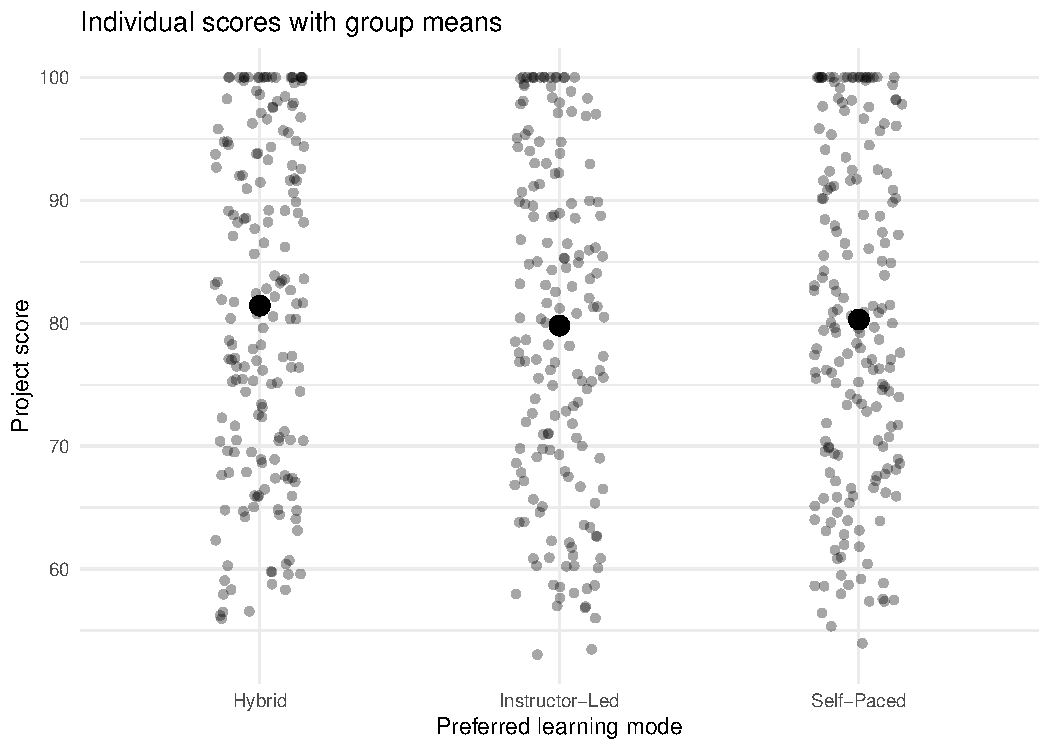
\includegraphics[width=0.9\linewidth,height=\textheight,keepaspectratio,alt={A layered plot showing individual points in the background and summary means drawn on top.}]{chapters/16-data-visualization_files/figure-pdf/fig-16-10-layer-order-1.pdf}

}

\caption{\label{fig-16-10-layer-order}A Layered Plot Where the Summary
Mean Is Drawn After the Individual Points.}

\end{figure}%

The code in Listing~\ref{lst-fig-16-10-layer-order} produces
Figure~\ref{fig-16-10-layer-order}.

The jittered points appear first. They show individual variation. The
mean points appear after them, so they are drawn on top.

If Leo reversed the order, the individual points could cover the summary
marks.

That is the layer rule:

\begin{quote}
In \texttt{ggplot2}, later layers are drawn over earlier layers.
\end{quote}

This is not only technical. It is part of visual reasoning. Leo decides
what should sit in the background and what should sit in the foreground.

\section{Basic Faceting: Small Multiples Without Losing the Main
Plot}\label{basic-faceting-small-multiples-without-losing-the-main-plot}

Sometimes one plot contains too many comparisons.

Leo may want to see whether the relationship between study hours and
project score differs across learner backgrounds or regions. He could
map another variable to colour, but too many colours can become hard to
read.

Faceting offers another option. It splits one plot into smaller panels.

The basic form is:

\begin{codelisting}

\caption{\label{lst-chapter16-facet-template}Code for Basic Faceting
Templates}

\centering{

\begin{Shaded}
\begin{Highlighting}[]
\FunctionTok{facet\_wrap}\NormalTok{(}\SpecialCharTok{\textasciitilde{}}\NormalTok{ background)}

\FunctionTok{facet\_grid}\NormalTok{(region }\SpecialCharTok{\textasciitilde{}}\NormalTok{ preferred\_learning\_mode)}
\end{Highlighting}
\end{Shaded}

}

\end{codelisting}%

The code in Listing~\ref{lst-chapter16-facet-template} shows the basic
faceting templates Leo is about to use.

\texttt{facet\_wrap()} arranges panels for one faceting variable.

\texttt{facet\_grid()} arranges panels across rows and columns.

Leo begins with a simple faceted scatter plot.

\begin{codelisting}

\caption{\label{lst-fig-16-11-facet-wrap-background}Code for Study Hours
and Project Score Faceted by Learner Background}

\centering{

\begin{Shaded}
\begin{Highlighting}[]
\FunctionTok{ggplot}\NormalTok{(}
  \AttributeTok{data =}\NormalTok{ df\_plot,}
  \AttributeTok{mapping =} \FunctionTok{aes}\NormalTok{(}\AttributeTok{x =}\NormalTok{ study\_hours, }\AttributeTok{y =}\NormalTok{ project\_score)}
\NormalTok{) }\SpecialCharTok{+}
  \FunctionTok{geom\_point}\NormalTok{(}\AttributeTok{alpha =} \FloatTok{0.55}\NormalTok{) }\SpecialCharTok{+}
  \FunctionTok{facet\_wrap}\NormalTok{(}\SpecialCharTok{\textasciitilde{}}\NormalTok{ background) }\SpecialCharTok{+}
  \FunctionTok{labs}\NormalTok{(}
    \AttributeTok{title =} \StringTok{"Study hours and project score by learner background"}\NormalTok{,}
    \AttributeTok{x =} \StringTok{"Study hours"}\NormalTok{,}
    \AttributeTok{y =} \StringTok{"Project score"}
\NormalTok{  ) }\SpecialCharTok{+}
  \FunctionTok{theme\_minimal}\NormalTok{()}
\end{Highlighting}
\end{Shaded}

}

\end{codelisting}%

\begin{figure}[H]

\centering{

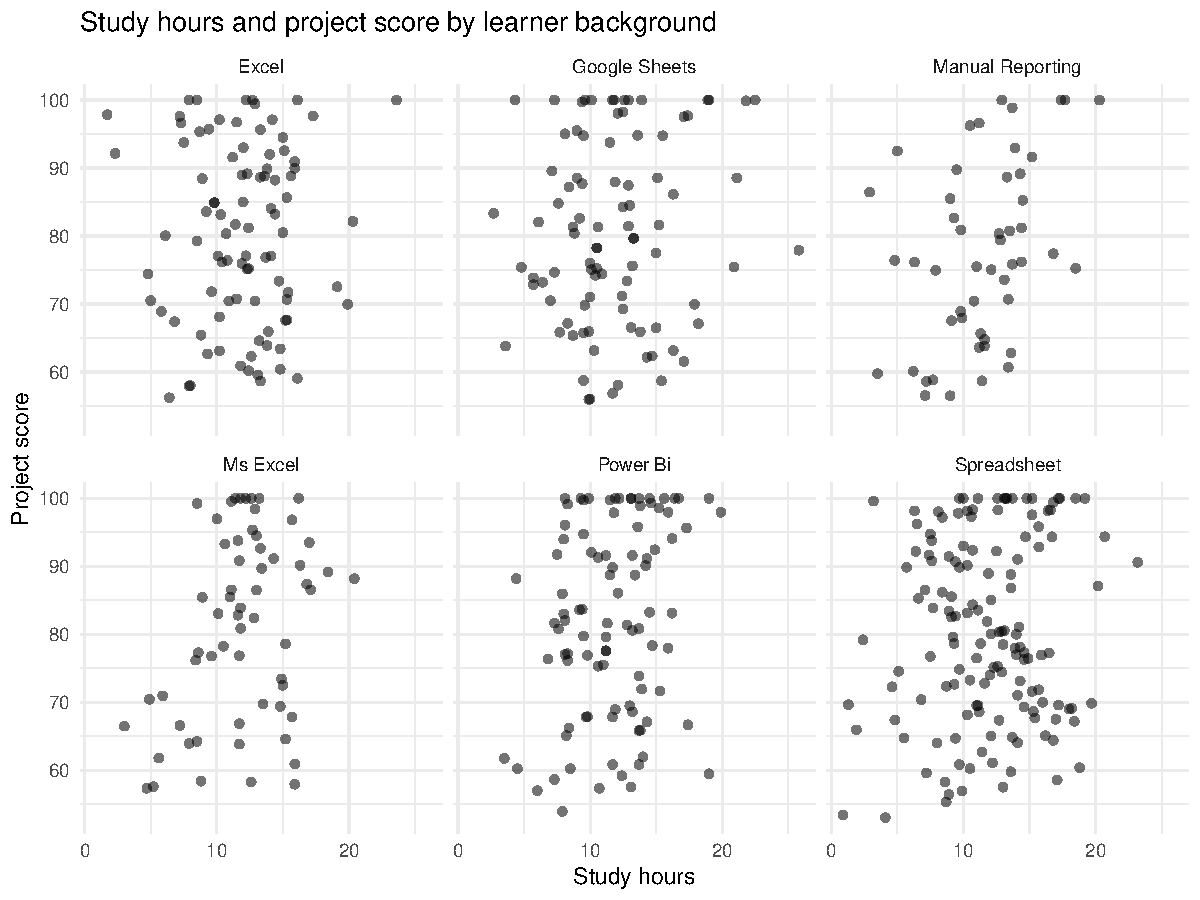
\includegraphics[width=0.9\linewidth,height=\textheight,keepaspectratio,alt={A faceted scatter plot showing study hours and project score separately for each learner background.}]{chapters/16-data-visualization_files/figure-pdf/fig-16-11-facet-wrap-background-1.pdf}

}

\caption{\label{fig-16-11-facet-wrap-background}Study Hours and Project
Score Faceted by Learner Background.}

\end{figure}%

The code in Listing~\ref{lst-fig-16-11-facet-wrap-background} produces
Figure~\ref{fig-16-11-facet-wrap-background}.

Faceting helps Leo compare patterns across groups while keeping the same
axes and visual grammar.

But faceting can also become too much. If there are too many categories,
the plot becomes a wall of small panels. Chapter 17 will return to this
issue through the lens of clarity and control. For now, Leo only needs
the basic idea: use facets when the same plot needs to be repeated
across groups.

Here is the basic grid version:

\begin{codelisting}

\caption{\label{lst-chapter16-facet-grid-example}Code for a
facet\_grid() Example}

\centering{

\begin{Shaded}
\begin{Highlighting}[]
\FunctionTok{ggplot}\NormalTok{(}
  \AttributeTok{data =}\NormalTok{ df\_plot,}
  \AttributeTok{mapping =} \FunctionTok{aes}\NormalTok{(}\AttributeTok{x =}\NormalTok{ study\_hours, }\AttributeTok{y =}\NormalTok{ project\_score)}
\NormalTok{) }\SpecialCharTok{+}
  \FunctionTok{geom\_point}\NormalTok{(}\AttributeTok{alpha =} \FloatTok{0.55}\NormalTok{) }\SpecialCharTok{+}
  \FunctionTok{facet\_grid}\NormalTok{(region }\SpecialCharTok{\textasciitilde{}}\NormalTok{ preferred\_learning\_mode)}
\end{Highlighting}
\end{Shaded}

}

\end{codelisting}%

\begin{figure}[H]

\centering{

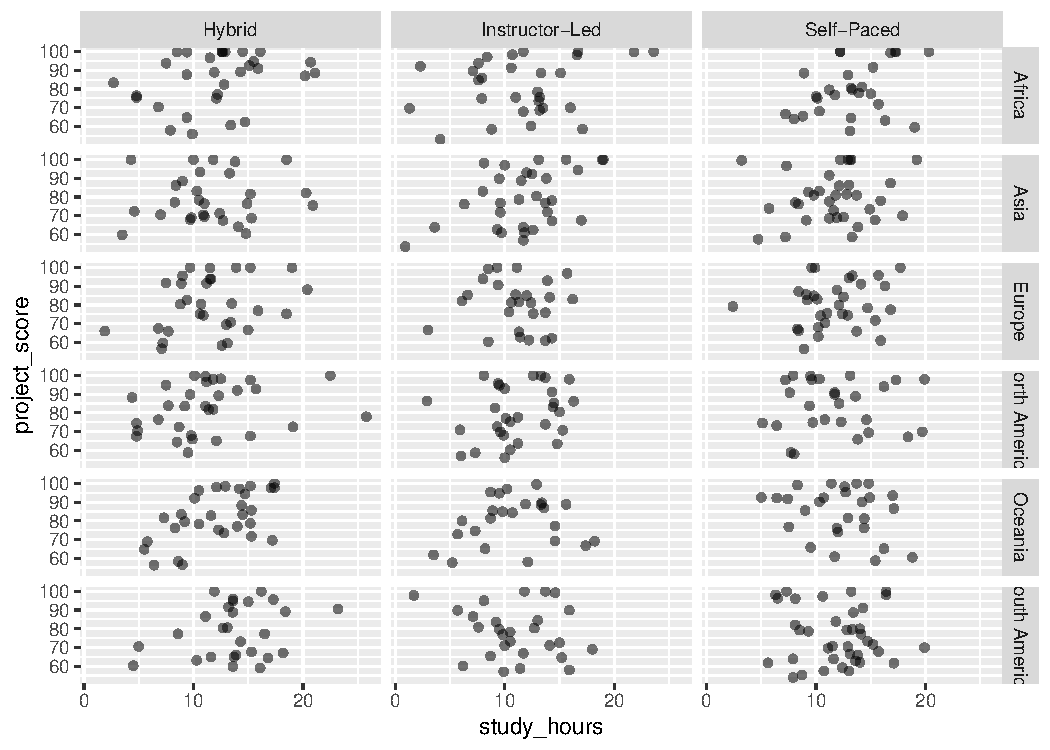
\includegraphics[width=0.9\linewidth,height=\textheight,keepaspectratio,alt={A faceted scatter plot of study hours and project score, arranged by region and preferred learning mode.}]{chapters/16-data-visualization_files/figure-pdf/fig-16-facet-grid-example-1.pdf}

}

\caption{\label{fig-16-facet-grid-example}Using facet\_grid() to Compare
Two Grouping Variables}

\end{figure}%

The code in Listing~\ref{lst-chapter16-facet-grid-example} produces
Figure~\ref{fig-16-facet-grid-example}.

This can be useful when Leo wants to compare two grouping variables at
once. It should be used carefully because the number of panels can grow
quickly.

\section{Themes: Controlling Non-Data
Appearance}\label{themes-controlling-non-data-appearance}

A theme controls the parts of a plot that are not the data itself.

This includes background, grid lines, text size, legend position, panel
spacing, and other visual elements.

For beginners, one of the safest starting points is:

\begin{codelisting}

\caption{\label{lst-chapter16-theme-minimal}Code for Applying
theme\_minimal()}

\centering{

\begin{Shaded}
\begin{Highlighting}[]
\FunctionTok{theme\_minimal}\NormalTok{()}
\end{Highlighting}
\end{Shaded}

}

\end{codelisting}%

The code in Listing~\ref{lst-chapter16-theme-minimal} shows the basic
\texttt{theme\_minimal()} pattern.

Leo has already used it in several plots in this chapter. It reduces
visual heaviness without demanding a full design system.

Other built-in themes include:

\begin{codelisting}

\caption{\label{lst-chapter16-theme-examples}Code for Built-In ggplot2
Theme Examples}

\centering{

\begin{Shaded}
\begin{Highlighting}[]
\FunctionTok{theme\_classic}\NormalTok{()}
\FunctionTok{theme\_bw}\NormalTok{()}
\FunctionTok{theme\_light}\NormalTok{()}
\FunctionTok{theme\_void}\NormalTok{()}
\end{Highlighting}
\end{Shaded}

}

\end{codelisting}%

The code in Listing~\ref{lst-chapter16-theme-examples} lists other
built-in themes Leo may encounter.

This is where beginners often go too far. They try to make a plot
``beautiful'' before they make it clear. That is not the purpose of
themes in this chapter.

The practical rule is:

\begin{quote}
Use themes to reduce distraction, not to decorate weak analysis.
\end{quote}

Chapter 17 will show Leo how to refine visual clarity more deliberately.
Here, the important point is simply that theme choices affect
readability, but they do not change the data.

\section{Scales and Coordinate
Systems}\label{scales-and-coordinate-systems}

Scales control how data values become visual values.

Coordinates control the space in which the plot is drawn.

Leo has already seen scales without naming them. When
\texttt{study\_hours} goes on the x-axis, \texttt{ggplot2} creates an x
scale. When \texttt{completion\_status} becomes colour, \texttt{ggplot2}
creates a colour scale. When \texttt{project\_score} becomes height,
\texttt{ggplot2} creates a y scale.

Sometimes Leo needs to control those scales.

For example, he can format a y-axis as percentages when plotting
completion rates.

\begin{codelisting}

\caption{\label{lst-chapter16-completion-rate-summary}Code for Preparing
Completion Rates by Learner Background}

\centering{

\begin{Shaded}
\begin{Highlighting}[]
\NormalTok{df\_completion\_rate }\OtherTok{\textless{}{-}}\NormalTok{ df\_plot }\SpecialCharTok{|\textgreater{}}
  \FunctionTok{filter}\NormalTok{(}\SpecialCharTok{!}\FunctionTok{is.na}\NormalTok{(completed\_flag)) }\SpecialCharTok{|\textgreater{}}
  \FunctionTok{group\_by}\NormalTok{(background) }\SpecialCharTok{|\textgreater{}}
  \FunctionTok{summarise}\NormalTok{(}
    \AttributeTok{completion\_rate =} \FunctionTok{mean}\NormalTok{(completed\_flag),}
    \AttributeTok{learners =} \FunctionTok{n}\NormalTok{(),}
    \AttributeTok{.groups =} \StringTok{"drop"}
\NormalTok{  ) }\SpecialCharTok{|\textgreater{}}
  \FunctionTok{arrange}\NormalTok{(}\FunctionTok{desc}\NormalTok{(completion\_rate))}

\NormalTok{knitr}\SpecialCharTok{::}\FunctionTok{kable}\NormalTok{(df\_completion\_rate)}
\end{Highlighting}
\end{Shaded}

}

\end{codelisting}%

{

\begin{longtable}[]{@{}lrr@{}}

\caption{\label{tbl-16-completion-rate-summary}Completion Rates by
Learner Background Prepared for Plotting.}

\tabularnewline

\toprule\noalign{}
background & completion\_rate & learners \\
\midrule\noalign{}
\endhead
\bottomrule\noalign{}
\endlastfoot
Manual Reporting & 0.6750000 & 40 \\
Ms Excel & 0.6190476 & 42 \\
Power Bi & 0.5573770 & 61 \\
Spreadsheet & 0.5544554 & 101 \\
Google Sheets & 0.5081967 & 61 \\
Excel & 0.4500000 & 60 \\

\end{longtable}

}

The code in Listing~\ref{lst-chapter16-completion-rate-summary} creates
Table~\ref{tbl-16-completion-rate-summary}. The code in
Listing~\ref{lst-fig-16-12-scale-coordinate-completion-rate} uses that
prepared summary to produce
Figure~\ref{fig-16-12-scale-coordinate-completion-rate}.

\begin{codelisting}

\caption{\label{lst-fig-16-12-scale-coordinate-completion-rate}Code for
Completion Rate by Learner Background with a Percentage Scale and
Flipped Coordinates}

\centering{

\begin{Shaded}
\begin{Highlighting}[]
\FunctionTok{ggplot}\NormalTok{(}
  \AttributeTok{data =}\NormalTok{ df\_completion\_rate,}
  \AttributeTok{mapping =} \FunctionTok{aes}\NormalTok{(}\AttributeTok{x =}\NormalTok{ background, }\AttributeTok{y =}\NormalTok{ completion\_rate)}
\NormalTok{) }\SpecialCharTok{+}
  \FunctionTok{geom\_col}\NormalTok{() }\SpecialCharTok{+}
  \FunctionTok{scale\_y\_continuous}\NormalTok{(}
    \AttributeTok{labels =} \ControlFlowTok{function}\NormalTok{(x) }\FunctionTok{paste0}\NormalTok{(}\FunctionTok{round}\NormalTok{(x }\SpecialCharTok{*} \DecValTok{100}\NormalTok{), }\StringTok{"\%"}\NormalTok{),}
    \AttributeTok{limits =} \FunctionTok{c}\NormalTok{(}\DecValTok{0}\NormalTok{, }\DecValTok{1}\NormalTok{)}
\NormalTok{  ) }\SpecialCharTok{+}
  \FunctionTok{coord\_flip}\NormalTok{() }\SpecialCharTok{+}
  \FunctionTok{labs}\NormalTok{(}
    \AttributeTok{title =} \StringTok{"Completion rate by learner background"}\NormalTok{,}
    \AttributeTok{x =} \StringTok{"Learner background"}\NormalTok{,}
    \AttributeTok{y =} \StringTok{"Completion rate"}
\NormalTok{  ) }\SpecialCharTok{+}
  \FunctionTok{theme\_minimal}\NormalTok{()}
\end{Highlighting}
\end{Shaded}

}

\end{codelisting}%

\begin{figure}[H]

\centering{

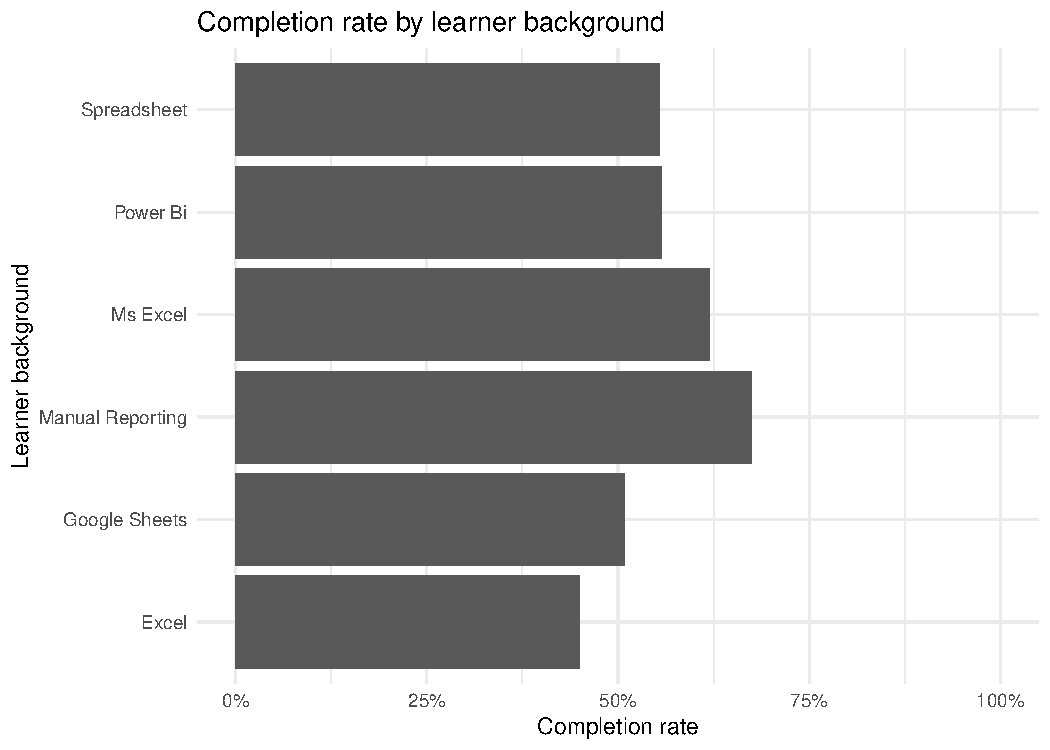
\includegraphics[width=0.9\linewidth,height=\textheight,keepaspectratio,alt={A horizontal bar chart showing completion rate by learner background with a percentage scale.}]{chapters/16-data-visualization_files/figure-pdf/fig-16-12-scale-coordinate-completion-rate-1.pdf}

}

\caption{\label{fig-16-12-scale-coordinate-completion-rate}Completion
Rate by Learner Background with a Percentage Scale and Flipped
Coordinates.}

\end{figure}%

The code in Listing~\ref{lst-fig-16-12-scale-coordinate-completion-rate}
produces Figure~\ref{fig-16-12-scale-coordinate-completion-rate}.

Two things changed here.

\texttt{scale\_y\_continuous()} controls how the numeric y-axis is
displayed. The data remain proportions, but the labels are shown as
percentages.

\texttt{coord\_flip()} switches the x and y axes visually. This can make
long category labels easier to read.

Leo should notice the boundary. Scales and coordinates change how the
data are displayed. They should not be used to mislead. A visual choice
that hides relevant variation or exaggerates a pattern weakens the
argument.

\section{Saving and Exporting Plots with
ggsave()}\label{saving-and-exporting-plots-with-ggsave}

A plot in the RStudio Plots pane is not yet a deliverable.

Leo will often need to save a figure for a report, slide, article, or
Quarto document. \texttt{ggplot2} provides \texttt{ggsave()} for this
task.

The safest habit is to assign the plot to an object and then save it.

\begin{codelisting}

\caption{\label{lst-chapter16-save-plot}Code for Saving a Named Plot
with ggsave()}

\centering{

\begin{Shaded}
\begin{Highlighting}[]
\NormalTok{completion\_plot }\OtherTok{\textless{}{-}} \FunctionTok{ggplot}\NormalTok{(}
  \AttributeTok{data =}\NormalTok{ df\_completion\_rate,}
  \AttributeTok{mapping =} \FunctionTok{aes}\NormalTok{(}\AttributeTok{x =}\NormalTok{ background, }\AttributeTok{y =}\NormalTok{ completion\_rate)}
\NormalTok{) }\SpecialCharTok{+}
  \FunctionTok{geom\_col}\NormalTok{() }\SpecialCharTok{+}
  \FunctionTok{scale\_y\_continuous}\NormalTok{(}
    \AttributeTok{labels =} \ControlFlowTok{function}\NormalTok{(x) }\FunctionTok{paste0}\NormalTok{(}\FunctionTok{round}\NormalTok{(x }\SpecialCharTok{*} \DecValTok{100}\NormalTok{), }\StringTok{"\%"}\NormalTok{),}
    \AttributeTok{limits =} \FunctionTok{c}\NormalTok{(}\DecValTok{0}\NormalTok{, }\DecValTok{1}\NormalTok{)}
\NormalTok{  ) }\SpecialCharTok{+}
  \FunctionTok{coord\_flip}\NormalTok{() }\SpecialCharTok{+}
  \FunctionTok{labs}\NormalTok{(}
    \AttributeTok{title =} \StringTok{"Completion rate by learner background"}\NormalTok{,}
    \AttributeTok{x =} \StringTok{"Learner background"}\NormalTok{,}
    \AttributeTok{y =} \StringTok{"Completion rate"}
\NormalTok{  ) }\SpecialCharTok{+}
  \FunctionTok{theme\_minimal}\NormalTok{()}

\FunctionTok{ggsave}\NormalTok{(}
  \AttributeTok{filename =} \StringTok{"outputs/figures/chapter16{-}completion{-}rate.png"}\NormalTok{,}
  \AttributeTok{plot =}\NormalTok{ completion\_plot,}
  \AttributeTok{width =} \DecValTok{7}\NormalTok{,}
  \AttributeTok{height =} \DecValTok{5}\NormalTok{,}
  \AttributeTok{dpi =} \DecValTok{300}
\NormalTok{)}
\end{Highlighting}
\end{Shaded}

}

\end{codelisting}%

The code in Listing~\ref{lst-chapter16-save-plot} shows how to save a
named plot with explicit size and resolution.

This code names the file, names the plot object, sets dimensions, and
specifies resolution.

That is much better than saving whatever happens to be in the plotting
window.

\begin{tcolorbox}[enhanced jigsaw, arc=.35mm, bottomrule=.15mm, breakable, colback=white, colframe=quarto-callout-tip-color-frame, left=2mm, leftrule=.75mm, opacityback=0, rightrule=.15mm, toprule=.15mm]
\begin{minipage}[t]{5.5mm}
\textcolor{quarto-callout-tip-color}{\faLightbulb}
\end{minipage}%
\begin{minipage}[t]{\textwidth - 5.5mm}

\vspace{-3mm}\textbf{Export plots deliberately}\vspace{3mm}

When a plot matters, save it with a clear filename, explicit width,
explicit height, and an appropriate resolution. Reproducible output
should not depend on the size of Leo's current RStudio window.

\end{minipage}%
\end{tcolorbox}

Later, when Leo works more deeply with Quarto, many figures will be
generated directly inside reports. Still, \texttt{ggsave()} remains
useful when he needs standalone image files.

\section{A Brief Look at Interactive
Visualization}\label{a-brief-look-at-interactive-visualization}

Not every plot is meant for print.

Sometimes a reader needs to hover over points, zoom into a region,
filter categories, or explore values dynamically. That is where
interactive visualization becomes useful.

One common route is \texttt{plotly}.

\begin{codelisting}

\caption{\label{lst-chapter16-plotly-example}Code for Converting a
ggplot2 Plot to plotly}

\centering{

\begin{Shaded}
\begin{Highlighting}[]
\FunctionTok{library}\NormalTok{(plotly)}

\NormalTok{p }\OtherTok{\textless{}{-}} \FunctionTok{ggplot}\NormalTok{(}
  \AttributeTok{data =}\NormalTok{ df\_plot,}
  \AttributeTok{mapping =} \FunctionTok{aes}\NormalTok{(}
    \AttributeTok{x =}\NormalTok{ study\_hours,}
    \AttributeTok{y =}\NormalTok{ project\_score,}
    \AttributeTok{color =}\NormalTok{ completion\_status,}
    \AttributeTok{text =}\NormalTok{ learner\_id}
\NormalTok{  )}
\NormalTok{) }\SpecialCharTok{+}
  \FunctionTok{geom\_point}\NormalTok{(}\AttributeTok{alpha =} \FloatTok{0.65}\NormalTok{) }\SpecialCharTok{+}
  \FunctionTok{labs}\NormalTok{(}
    \AttributeTok{title =} \StringTok{"Interactive study hours and project score"}\NormalTok{,}
    \AttributeTok{x =} \StringTok{"Study hours"}\NormalTok{,}
    \AttributeTok{y =} \StringTok{"Project score"}
\NormalTok{  ) }\SpecialCharTok{+}
  \FunctionTok{theme\_minimal}\NormalTok{()}

\FunctionTok{ggplotly}\NormalTok{(p)}
\end{Highlighting}
\end{Shaded}

}

\end{codelisting}%

The code in Listing~\ref{lst-chapter16-plotly-example} shows how a
\texttt{ggplot2} object can be converted into an interactive
\texttt{plotly} object.

This takes a \texttt{ggplot2} object and turns it into an interactive
plot. A reader can hover, zoom, and inspect values.

Another route is Shiny, which builds interactive applications.

\begin{codelisting}

\caption{\label{lst-chapter16-shiny-sketch}Code for a Small Shiny App
Sketch}

\centering{

\begin{Shaded}
\begin{Highlighting}[]
\FunctionTok{library}\NormalTok{(shiny)}

\NormalTok{ui }\OtherTok{\textless{}{-}} \FunctionTok{fluidPage}\NormalTok{(}
  \FunctionTok{selectInput}\NormalTok{(}
    \AttributeTok{inputId =} \StringTok{"mode"}\NormalTok{,}
    \AttributeTok{label =} \StringTok{"Choose learning mode"}\NormalTok{,}
    \AttributeTok{choices =} \FunctionTok{unique}\NormalTok{(df\_plot}\SpecialCharTok{$}\NormalTok{preferred\_learning\_mode)}
\NormalTok{  ),}
  \FunctionTok{plotOutput}\NormalTok{(}\StringTok{"score\_plot"}\NormalTok{)}
\NormalTok{)}

\NormalTok{server }\OtherTok{\textless{}{-}} \ControlFlowTok{function}\NormalTok{(input, output, session) \{}
\NormalTok{  output}\SpecialCharTok{$}\NormalTok{score\_plot }\OtherTok{\textless{}{-}} \FunctionTok{renderPlot}\NormalTok{(\{}
\NormalTok{    df\_plot }\SpecialCharTok{|\textgreater{}}
      \FunctionTok{filter}\NormalTok{(preferred\_learning\_mode }\SpecialCharTok{==}\NormalTok{ input}\SpecialCharTok{$}\NormalTok{mode) }\SpecialCharTok{|\textgreater{}}
      \FunctionTok{ggplot}\NormalTok{(}\FunctionTok{aes}\NormalTok{(}\AttributeTok{x =}\NormalTok{ study\_hours, }\AttributeTok{y =}\NormalTok{ project\_score)) }\SpecialCharTok{+}
      \FunctionTok{geom\_point}\NormalTok{() }\SpecialCharTok{+}
      \FunctionTok{theme\_minimal}\NormalTok{()}
\NormalTok{  \})}
\NormalTok{\}}

\FunctionTok{shinyApp}\NormalTok{(ui, server)}
\end{Highlighting}
\end{Shaded}

}

\end{codelisting}%

The code in Listing~\ref{lst-chapter16-shiny-sketch} sketches the basic
structure of a small Shiny application.

This is only a glimpse. Shiny belongs to a larger topic: building
applications around analysis. Leo does not need to master it here.

The key boundary is this:

\begin{itemize}
\tightlist
\item
  \texttt{ggplot2} builds the visual argument
\item
  \texttt{plotly} can make plots interactive
\item
  Shiny can build interactive tools around plots and data
\end{itemize}

For Chapter 16, the goal is still the foundation: build a correct,
readable static plot first. Interactivity should not be used to rescue a
confusing design.

\section{Common Plot Problems and How to Diagnose
Them}\label{common-plot-problems-and-how-to-diagnose-them}

Many plotting errors are not really plotting errors. They are data,
type, structure, or logic problems showing up visually.

Leo can use the same debugging discipline he has built across the book.

\begin{codelisting}

\caption{\label{lst-tbl-16-3-plot-diagnosis}Code for Common Plotting
Problems and Practical Diagnosis Steps}

\centering{

\begin{Shaded}
\begin{Highlighting}[]
\NormalTok{tibble}\SpecialCharTok{::}\FunctionTok{tribble}\NormalTok{(}
  \SpecialCharTok{\textasciitilde{}}\NormalTok{Problem, }\SpecialCharTok{\textasciitilde{}}\NormalTok{Likely\_cause, }\SpecialCharTok{\textasciitilde{}}\NormalTok{What\_Leo\_should\_check,}
  \StringTok{"The plot is blank."}\NormalTok{, }\StringTok{"Filtered data may have zero rows, or required values may be missing."}\NormalTok{, }\StringTok{"Run nrow() and count missing values in mapped variables."}\NormalTok{,}
  \StringTok{"A numeric axis behaves like categories."}\NormalTok{, }\StringTok{"The variable may have been imported as character."}\NormalTok{, }\StringTok{"Check class() or glimpse(), then convert carefully if appropriate."}\NormalTok{,}
  \StringTok{"A bar chart shows duplicate{-}looking categories."}\NormalTok{, }\StringTok{"Text values may differ by spelling, case, or spaces."}\NormalTok{, }\StringTok{"Use count() to inspect categories and standardise text values."}\NormalTok{,}
  \StringTok{"A line connects categories in a strange order."}\NormalTok{, }\StringTok{"The x{-}axis may not be a meaningful ordered variable."}\NormalTok{, }\StringTok{"Use a line only when the x variable has sequence or time meaning."}\NormalTok{,}
  \StringTok{"Colours do not represent groups."}\NormalTok{, }\StringTok{"A fixed colour may have been set outside aes(), or a variable may be mapped incorrectly."}\NormalTok{, }\StringTok{"Decide whether the colour should be mapped or set."}\NormalTok{,}
  \StringTok{"A faceted plot has too many panels."}\NormalTok{, }\StringTok{"The faceting variable may have too many categories."}\NormalTok{, }\StringTok{"Reduce categories, filter the plot, or use a simpler comparison."}\NormalTok{,}
  \StringTok{"The saved figure looks distorted."}\NormalTok{, }\StringTok{"The export dimensions or resolution were not specified."}\NormalTok{, }\StringTok{"Use ggsave() with width, height, and dpi."}
\NormalTok{) }\SpecialCharTok{|\textgreater{}}
\NormalTok{  knitr}\SpecialCharTok{::}\FunctionTok{kable}\NormalTok{()}
\end{Highlighting}
\end{Shaded}

}

\end{codelisting}%

{

\begin{longtable}[]{@{}
  >{\raggedright\arraybackslash}p{(\linewidth - 4\tabcolsep) * \real{0.2353}}
  >{\raggedright\arraybackslash}p{(\linewidth - 4\tabcolsep) * \real{0.4363}}
  >{\raggedright\arraybackslash}p{(\linewidth - 4\tabcolsep) * \real{0.3284}}@{}}

\caption{\label{tbl-16-3-plot-diagnosis}Common Plotting Problems and
Practical Diagnosis Steps.}

\tabularnewline

\toprule\noalign{}
\begin{minipage}[b]{\linewidth}\raggedright
Problem
\end{minipage} & \begin{minipage}[b]{\linewidth}\raggedright
Likely\_cause
\end{minipage} & \begin{minipage}[b]{\linewidth}\raggedright
What\_Leo\_should\_check
\end{minipage} \\
\midrule\noalign{}
\endhead
\bottomrule\noalign{}
\endlastfoot
The plot is blank. & Filtered data may have zero rows, or required
values may be missing. & Run nrow() and count missing values in mapped
variables. \\
A numeric axis behaves like categories. & The variable may have been
imported as character. & Check class() or glimpse(), then convert
carefully if appropriate. \\
A bar chart shows duplicate-looking categories. & Text values may differ
by spelling, case, or spaces. & Use count() to inspect categories and
standardise text values. \\
A line connects categories in a strange order. & The x-axis may not be a
meaningful ordered variable. & Use a line only when the x variable has
sequence or time meaning. \\
Colours do not represent groups. & A fixed colour may have been set
outside aes(), or a variable may be mapped incorrectly. & Decide whether
the colour should be mapped or set. \\
A faceted plot has too many panels. & The faceting variable may have too
many categories. & Reduce categories, filter the plot, or use a simpler
comparison. \\
The saved figure looks distorted. & The export dimensions or resolution
were not specified. & Use ggsave() with width, height, and dpi. \\

\end{longtable}

}

The code in Listing~\ref{lst-tbl-16-3-plot-diagnosis} creates
Table~\ref{tbl-16-3-plot-diagnosis}.

This table should feel familiar. It is the same mental discipline from
earlier chapters:

\begin{itemize}
\tightlist
\item
  check syntax
\item
  check the object
\item
  check the type
\item
  check the structure
\item
  check the logic
\end{itemize}

Plotting has its own vocabulary, but it does not require a new
personality. Leo still works patiently from evidence to explanation.

\section{What Leo Can Now Do}\label{what-leo-can-now-do}

Leo began this chapter with a table that was correct but slow to
interpret.

He now understands why a plot is not a magic picture produced by R. It
is a deliberate construction.

He can choose a data frame, map variables to visual attributes, add
geometric layers, distinguish mapping from setting, use counts and bins,
calculate or display summaries, group patterns correctly, draw layers in
a meaningful order, split a plot into facets, apply basic themes,
control scales and coordinates, and export a plot with
\texttt{ggsave()}.

That is a major step.

But Leo also sees the next problem.

A technically correct plot is not always a clear plot.

A plot can use the right variables and still bury the point. It can have
the right geom and still use confusing labels. It can show the right
summary and still make the reader work too hard.

That is why Chapter 17 moves from making plots to controlling what
readers actually see.

\section{Chapter Outcome}\label{chapter-outcome-15}

By the end of this chapter, Leo can:

\begin{itemize}
\tightlist
\item
  explain why visualization depends on cleaned and analysis-ready data
\item
  recognise the difference between base R graphics, \texttt{lattice},
  \texttt{plotly}, Shiny, and \texttt{ggplot2}
\item
  describe the grammar of graphics in practical terms
\item
  build basic \texttt{ggplot2} plots from data frames
\item
  use \texttt{aes()} to map variables to visual attributes
\item
  distinguish mapping from setting
\item
  choose between \texttt{geom\_point()}, \texttt{geom\_line()},
  \texttt{geom\_bar()}, \texttt{geom\_col()}, and
  \texttt{geom\_histogram()}
\item
  explain the difference between continuous and discrete scales
\item
  use grouping to draw several patterns in one plot
\item
  understand basic statistical transformations such as counts, bins, and
  means
\item
  control basic layer order
\item
  use simple faceting with \texttt{facet\_wrap()} and
  \texttt{facet\_grid()}
\item
  apply basic themes, scales, and coordinate changes
\item
  save plots deliberately with \texttt{ggsave()}
\item
  recognise when interactivity belongs to \texttt{plotly} or Shiny
  rather than basic static plotting
\end{itemize}

\section{Chapter Design Principle}\label{chapter-design-principle}

Show the structure behind the picture.

Leo has moved from summarising evidence to seeing evidence.

Next, he will learn how to make that evidence clearer.

\section{References}\label{references}

Chang, W., Cheng, J., Allaire, J. J., Sievert, C., Schloerke, B.,
Aden-Buie, G., Xie, Y., Allen, J., McPherson, J., Dipert, A., Borges,
B., \& Posit Software, PBC. (2026). \emph{shiny: Web application
framework for R} (R package).
https://doi.org/10.32614/CRAN.package.shiny

Cleveland, W. S. (1993). \emph{Visualizing data}. Hobart Press.

Healy, K. (2019). \emph{Data visualization: A practical introduction}.
Princeton University Press.

Sarkar, D. (2008). \emph{Lattice: Multivariate data visualization with
R}. Springer. https://doi.org/10.1007/978-0-387-75969-2

Sievert, C. (2020). \emph{Interactive web-based data visualization with
R, plotly, and shiny}. Chapman and Hall/CRC.
https://doi.org/10.1201/9780429447273

Wickham, H. (2016). \emph{ggplot2: Elegant graphics for data analysis}
(2nd ed.). Springer. https://doi.org/10.1007/978-3-319-24277-4

Wickham, H., Çetinkaya-Rundel, M., \& Grolemund, G. (2023). \emph{R for
data science} (2nd ed.). O'Reilly Media. https://r4ds.hadley.nz/

Wilkinson, L. (2005). \emph{The grammar of graphics} (2nd ed.).
Springer. https://doi.org/10.1007/0-387-28695-0

\chapter{Clarity and Control: Designing Visualisations People Can
Understand}\label{clarity-and-control-designing-visualisations-people-can-understand}

\renewcommand{\thefigure}{17.\arabic{figure}}
\setcounter{figure}{0}
\renewcommand{\thetable}{17.\arabic{table}}
\setcounter{table}{0}

\begin{tcolorbox}[enhanced jigsaw, arc=.35mm, bottomrule=.15mm, breakable, colback=white, colframe=quarto-callout-note-color-frame, left=2mm, leftrule=.75mm, opacityback=0, rightrule=.15mm, toprule=.15mm]
\begin{minipage}[t]{5.5mm}
\textcolor{quarto-callout-note-color}{\faInfo}
\end{minipage}%
\begin{minipage}[t]{\textwidth - 5.5mm}

\vspace{-3mm}\textbf{Data used in this chapter}\vspace{3mm}

This chapter continues with the same
\texttt{df\_r\_migration\_messy.csv} teaching dataset introduced in Part
3 and reused at the start of Part 4. If you are reading this chapter
directly, first make sure the file is available at
\texttt{data/raw/df\_r\_migration\_messy.csv} or
\texttt{datasets/raw/df\_r\_migration\_messy.csv}.

\end{minipage}%
\end{tcolorbox}

\section{Opening Scene: When a Correct Plot Still
Fails}\label{opening-scene-when-a-correct-plot-still-fails}

Leo has reached the point many new R users are desperate to reach.

He can import data. He can clean it. He can select variables, filter
rows, create new columns, summarise groups, and build plots with
\texttt{ggplot2}. After the long climb through Part 3 and the opening
chapter of Part 4, he finally has something that looks like analytical
output.

One afternoon, he prepares a plot for a short team meeting. The code
runs. No error appears. The plot shows the relationship between weekly
study hours and project scores in the learner dataset. Leo feels ready.

Then the questions begin.

One colleague asks, ``Which group am I supposed to look at first?''

Another says, ``The legend is confusing. Are these colours important?''

Someone else points at the scatter plot and says, ``There are too many
points. I cannot see the pattern.''

A fourth person notices that the labels overlap so badly that the most
important countries are almost unreadable.

Leo looks again. The plot is not wrong. The data are there. The code is
valid. The chart appears on the screen exactly as R was asked to draw
it.

But the plot has failed its reader.

That failure matters. In real analytical work, correctness is not
enough. A chart can be technically correct and still hide the pattern,
distract the eye, exaggerate a difference, bury the comparison, or make
the reader work too hard.

This chapter begins from that uncomfortable but liberating truth:

\begin{quote}
A chart is not finished when the data appears.\\
A chart is finished when the intended pattern becomes easy to see.
\end{quote}

Chapter 16 taught Leo how to turn data into pictures. Chapter 17 teaches
him how to take control of those pictures so they become readable,
honest, and useful.

\begin{tcolorbox}[enhanced jigsaw, arc=.35mm, bottomrule=.15mm, breakable, colback=white, colframe=quarto-callout-note-color-frame, left=2mm, leftrule=.75mm, opacityback=0, rightrule=.15mm, toprule=.15mm]
\begin{minipage}[t]{5.5mm}
\textcolor{quarto-callout-note-color}{\faInfo}
\end{minipage}%
\begin{minipage}[t]{\textwidth - 5.5mm}

\vspace{-3mm}\textbf{Chapter Compass}\vspace{3mm}

In this chapter, Leo learns how to refine visualisations with purpose.
He will control scales, colours, themes, text, legends, labels,
annotations, aspect ratios, zooming, overplotting, multi-panel layouts,
and simple interactivity. The goal is not decoration. The goal is visual
control: making the intended comparison easier to see without damaging
the evidence.

Chapter 18 will move from clear plots to visual storytelling. This
chapter stays with the plot itself: what is visible, what is cluttered,
what is emphasized, and what the reader can understand without
struggling.

\end{minipage}%
\end{tcolorbox}

\section{What Changed After Chapter
16}\label{what-changed-after-chapter-16}

Chapter 16 gave Leo the grammar of basic visualisation in R. He learned
that a \texttt{ggplot2} chart is built from data, aesthetics, geometric
layers, and supporting choices such as labels and themes. He also
learned a crucial principle: plot type follows analytical question.

Chapter 17 assumes that foundation. It does not restart the lesson on
what \texttt{ggplot()} means. It does not reintroduce every geom. It
does not ask Leo to memorize a gallery of chart types.

Instead, it asks a more professional question:

\begin{quote}
Once the plot exists, what must be controlled so the evidence becomes
easier to read?
\end{quote}

That question changes Leo's relationship with visualisation. He is no
longer asking only, ``How do I make a scatter plot?'' He is asking:

\begin{itemize}
\tightlist
\item
  Is the pattern visible?
\item
  Are the labels meaningful?
\item
  Are the scales honest?
\item
  Does colour carry information or merely decorate?
\item
  Is the legend helping or creating extra work?
\item
  Are labels colliding?
\item
  Is the plot too crowded?
\item
  Does the layout guide the eye?
\item
  Would interactivity help the reader explore details that cannot fit
  cleanly in a static figure?
\end{itemize}

These are clarity-and-control questions. They are also analytical
questions.

A plot is a claim about what matters in the data. If the design makes
that claim hard to see, the analysis loses force.

\section{Why Good Charts Fail}\label{why-good-charts-fail}

Good charts usually fail for ordinary reasons. They fail because the
default settings were treated as final. They fail because too much
information was pushed into one panel. They fail because colours were
added before the purpose of colour was clear. They fail because labels
were placed where R could fit them, not where readers could understand
them.

The first step toward control is recognizing the failure pattern.

\begin{codelisting}

\caption{\label{lst-tbl-17-1}Code for 17 1}

\centering{

\begin{Shaded}
\begin{Highlighting}[]
\NormalTok{clarity\_failures }\OtherTok{\textless{}{-}}\NormalTok{ tibble}\SpecialCharTok{::}\FunctionTok{tribble}\NormalTok{(}
  \SpecialCharTok{\textasciitilde{}}\NormalTok{Problem, }\SpecialCharTok{\textasciitilde{}}\StringTok{\textasciigrave{}}\AttributeTok{How it appears}\StringTok{\textasciigrave{}}\NormalTok{, }\SpecialCharTok{\textasciitilde{}}\StringTok{\textasciigrave{}}\AttributeTok{Practical way out}\StringTok{\textasciigrave{}}\NormalTok{,}
  \StringTok{"Unclear visual question"}\NormalTok{, }\StringTok{"The chart shows data but does not guide interpretation"}\NormalTok{, }\StringTok{"Write the plot question before refining the design"}\NormalTok{,}
  \StringTok{"Overplotting"}\NormalTok{, }\StringTok{"Points sit on top of one another and hide density"}\NormalTok{, }\StringTok{"Use alpha blending, jittering, binning, or hexagonal bins"}\NormalTok{,}
  \StringTok{"Confusing legend"}\NormalTok{, }\StringTok{"The reader must constantly move between plot and legend"}\NormalTok{, }\StringTok{"Simplify the legend, move it, rename it, or use direct labels"}\NormalTok{,}
  \StringTok{"Weak scale control"}\NormalTok{, }\StringTok{"Axis breaks, limits, or labels make comparison difficult"}\NormalTok{, }\StringTok{"Use scale\_x\_*(), scale\_y\_*(), breaks, labels, or coord\_cartesian()"}\NormalTok{,}
  \StringTok{"Poor colour choice"}\NormalTok{, }\StringTok{"Colour distracts, excludes, or implies false meaning"}\NormalTok{, }\StringTok{"Use colour only for meaning and prefer accessible palettes"}\NormalTok{,}
  \StringTok{"Label collision"}\NormalTok{, }\StringTok{"Important labels overlap and become unreadable"}\NormalTok{, }\StringTok{"Use ggrepel or reduce the number of labels"}\NormalTok{,}
  \StringTok{"Crowded facets"}\NormalTok{, }\StringTok{"Small panels become too cramped to read"}\NormalTok{, }\StringTok{"Reduce groups, adjust spacing, or use patchwork for controlled layouts"}\NormalTok{,}
  \StringTok{"Rigid text formatting"}\NormalTok{, }\StringTok{"Titles, subtitles, annotations, or equations look awkward"}\NormalTok{, }\StringTok{"Use element\_text(), expression(), annotate(), or ggtext"}\NormalTok{,}
  \StringTok{"Distorted aspect ratio"}\NormalTok{, }\StringTok{"The same pattern looks steeper, flatter, or more dramatic than it is"}\NormalTok{, }\StringTok{"Control aspect ratio with theme(aspect.ratio = ) or coord\_fixed()"}\NormalTok{,}
  \StringTok{"Static plot doing interactive work"}\NormalTok{, }\StringTok{"Too many details are forced into labels or notes"}\NormalTok{, }\StringTok{"Use plotly or ggiraph when hover{-}based exploration is appropriate"}
\NormalTok{)}

\NormalTok{knitr}\SpecialCharTok{::}\FunctionTok{kable}\NormalTok{(clarity\_failures)}
\end{Highlighting}
\end{Shaded}

}

\end{codelisting}%

{

\begin{longtable}[]{@{}
  >{\raggedright\arraybackslash}p{(\linewidth - 4\tabcolsep) * \real{0.2000}}
  >{\raggedright\arraybackslash}p{(\linewidth - 4\tabcolsep) * \real{0.3943}}
  >{\raggedright\arraybackslash}p{(\linewidth - 4\tabcolsep) * \real{0.4057}}@{}}

\caption{\label{tbl-17-1}Common Causes of Poor Visual Communication in
R}

\tabularnewline

\toprule\noalign{}
\begin{minipage}[b]{\linewidth}\raggedright
Problem
\end{minipage} & \begin{minipage}[b]{\linewidth}\raggedright
How it appears
\end{minipage} & \begin{minipage}[b]{\linewidth}\raggedright
Practical way out
\end{minipage} \\
\midrule\noalign{}
\endhead
\bottomrule\noalign{}
\endlastfoot
Unclear visual question & The chart shows data but does not guide
interpretation & Write the plot question before refining the design \\
Overplotting & Points sit on top of one another and hide density & Use
alpha blending, jittering, binning, or hexagonal bins \\
Confusing legend & The reader must constantly move between plot and
legend & Simplify the legend, move it, rename it, or use direct
labels \\
Weak scale control & Axis breaks, limits, or labels make comparison
difficult & Use scale\_x\_\emph{(), scale\_y\_}(), breaks, labels, or
coord\_cartesian() \\
Poor colour choice & Colour distracts, excludes, or implies false
meaning & Use colour only for meaning and prefer accessible palettes \\
Label collision & Important labels overlap and become unreadable & Use
ggrepel or reduce the number of labels \\
Crowded facets & Small panels become too cramped to read & Reduce
groups, adjust spacing, or use patchwork for controlled layouts \\
Rigid text formatting & Titles, subtitles, annotations, or equations
look awkward & Use element\_text(), expression(), annotate(), or
ggtext \\
Distorted aspect ratio & The same pattern looks steeper, flatter, or
more dramatic than it is & Control aspect ratio with theme(aspect.ratio
= ) or coord\_fixed() \\
Static plot doing interactive work & Too many details are forced into
labels or notes & Use plotly or ggiraph when hover-based exploration is
appropriate \\

\end{longtable}

}

The code in Listing~\ref{lst-tbl-17-1} produces Table~\ref{tbl-17-1}.

Table 17.1 gives Leo a diagnostic map. It is deliberately practical.
When a plot fails, the question is not, ``How do I make it beautiful?''
The better question is, ``What is preventing the reader from seeing the
intended pattern?''

That question leads to the framework for this chapter.

\section{The Clarity-Control
Framework}\label{the-clarity-control-framework}

Clarity and control are connected, but they are not the same thing.

\textbf{Clarity} is what the reader experiences. A clear plot makes the
intended pattern easy to see.

\textbf{Control} is what the analyst does. A controlled plot uses
scales, labels, colour, layout, and supporting elements deliberately.

Leo can think of visual refinement through five linked dimensions:

\begin{enumerate}
\def\labelenumi{\arabic{enumi}.}
\tightlist
\item
  \textbf{Visibility:} Can the reader see the pattern?
\item
  \textbf{Emphasis:} Does the plot guide attention to what matters?
\item
  \textbf{Structure:} Are comparisons arranged in a sensible order?
\item
  \textbf{Guidance:} Do labels, captions, legends, and annotations help
  interpretation?
\item
  \textbf{Consistency:} Do design choices behave predictably across
  related plots?
\end{enumerate}

\begin{codelisting}

\caption{\label{lst-fig-17-1}Code for 17 1}

\centering{

\begin{Shaded}
\begin{Highlighting}[]
\NormalTok{framework }\OtherTok{\textless{}{-}}\NormalTok{ tibble}\SpecialCharTok{::}\FunctionTok{tribble}\NormalTok{(}
  \SpecialCharTok{\textasciitilde{}}\NormalTok{dimension, }\SpecialCharTok{\textasciitilde{}}\NormalTok{x, }\SpecialCharTok{\textasciitilde{}}\NormalTok{y, }\SpecialCharTok{\textasciitilde{}}\NormalTok{short\_label,}
  \StringTok{"Visibility"}\NormalTok{, }\DecValTok{1}\NormalTok{, }\DecValTok{3}\NormalTok{, }\StringTok{"Can readers}\SpecialCharTok{\textbackslash{}n}\StringTok{see it?"}\NormalTok{,}
  \StringTok{"Emphasis"}\NormalTok{, }\DecValTok{3}\NormalTok{, }\DecValTok{3}\NormalTok{, }\StringTok{"Do they know}\SpecialCharTok{\textbackslash{}n}\StringTok{where to look?"}\NormalTok{,}
  \StringTok{"Structure"}\NormalTok{, }\DecValTok{5}\NormalTok{, }\DecValTok{3}\NormalTok{, }\StringTok{"Are comparisons}\SpecialCharTok{\textbackslash{}n}\StringTok{organized?"}\NormalTok{,}
  \StringTok{"Guidance"}\NormalTok{, }\DecValTok{2}\NormalTok{, }\DecValTok{1}\NormalTok{, }\StringTok{"Do labels}\SpecialCharTok{\textbackslash{}n}\StringTok{help?"}\NormalTok{,}
  \StringTok{"Consistency"}\NormalTok{, }\DecValTok{4}\NormalTok{, }\DecValTok{1}\NormalTok{, }\StringTok{"Do choices}\SpecialCharTok{\textbackslash{}n}\StringTok{repeat logically?"}
\NormalTok{)}

\NormalTok{connections }\OtherTok{\textless{}{-}}\NormalTok{ tibble}\SpecialCharTok{::}\FunctionTok{tribble}\NormalTok{(}
  \SpecialCharTok{\textasciitilde{}}\NormalTok{x, }\SpecialCharTok{\textasciitilde{}}\NormalTok{y, }\SpecialCharTok{\textasciitilde{}}\NormalTok{xend, }\SpecialCharTok{\textasciitilde{}}\NormalTok{yend,}
  \DecValTok{1}\NormalTok{, }\DecValTok{3}\NormalTok{, }\DecValTok{3}\NormalTok{, }\DecValTok{3}\NormalTok{,}
  \DecValTok{3}\NormalTok{, }\DecValTok{3}\NormalTok{, }\DecValTok{5}\NormalTok{, }\DecValTok{3}\NormalTok{,}
  \DecValTok{3}\NormalTok{, }\DecValTok{3}\NormalTok{, }\DecValTok{2}\NormalTok{, }\DecValTok{1}\NormalTok{,}
  \DecValTok{3}\NormalTok{, }\DecValTok{3}\NormalTok{, }\DecValTok{4}\NormalTok{, }\DecValTok{1}\NormalTok{,}
  \DecValTok{2}\NormalTok{, }\DecValTok{1}\NormalTok{, }\DecValTok{4}\NormalTok{, }\DecValTok{1}
\NormalTok{)}

\FunctionTok{ggplot}\NormalTok{() }\SpecialCharTok{+}
  \FunctionTok{geom\_segment}\NormalTok{(}
    \AttributeTok{data =}\NormalTok{ connections,}
    \FunctionTok{aes}\NormalTok{(}\AttributeTok{x =}\NormalTok{ x, }\AttributeTok{y =}\NormalTok{ y, }\AttributeTok{xend =}\NormalTok{ xend, }\AttributeTok{yend =}\NormalTok{ yend),}
    \AttributeTok{linewidth =} \FloatTok{0.5}\NormalTok{,}
    \AttributeTok{arrow =} \FunctionTok{arrow}\NormalTok{(}\AttributeTok{length =} \FunctionTok{unit}\NormalTok{(}\FloatTok{0.12}\NormalTok{, }\StringTok{"inches"}\NormalTok{))}
\NormalTok{  ) }\SpecialCharTok{+}
  \FunctionTok{geom\_label}\NormalTok{(}
    \AttributeTok{data =}\NormalTok{ framework,}
    \FunctionTok{aes}\NormalTok{(}\AttributeTok{x =}\NormalTok{ x, }\AttributeTok{y =}\NormalTok{ y, }\AttributeTok{label =}\NormalTok{ short\_label),}
    \AttributeTok{label.size =} \FloatTok{0.2}\NormalTok{,}
    \AttributeTok{size =} \FloatTok{3.7}\NormalTok{,}
    \AttributeTok{fontface =} \StringTok{"bold"}
\NormalTok{  ) }\SpecialCharTok{+}
  \FunctionTok{annotate}\NormalTok{(}
    \StringTok{"text"}\NormalTok{,}
    \AttributeTok{x =} \DecValTok{3}\NormalTok{,}
    \AttributeTok{y =} \DecValTok{4}\NormalTok{,}
    \AttributeTok{label =} \StringTok{"A chart is finished when the intended pattern becomes easy to see."}\NormalTok{,}
    \AttributeTok{fontface =} \StringTok{"bold"}\NormalTok{,}
    \AttributeTok{size =} \DecValTok{4}
\NormalTok{  ) }\SpecialCharTok{+}
  \FunctionTok{coord\_cartesian}\NormalTok{(}\AttributeTok{xlim =} \FunctionTok{c}\NormalTok{(}\FloatTok{0.4}\NormalTok{, }\FloatTok{5.6}\NormalTok{), }\AttributeTok{ylim =} \FunctionTok{c}\NormalTok{(}\FloatTok{0.3}\NormalTok{, }\FloatTok{4.4}\NormalTok{)) }\SpecialCharTok{+}
  \FunctionTok{theme\_void}\NormalTok{()}
\end{Highlighting}
\end{Shaded}

}

\end{codelisting}%

\begin{figure}[H]

\centering{

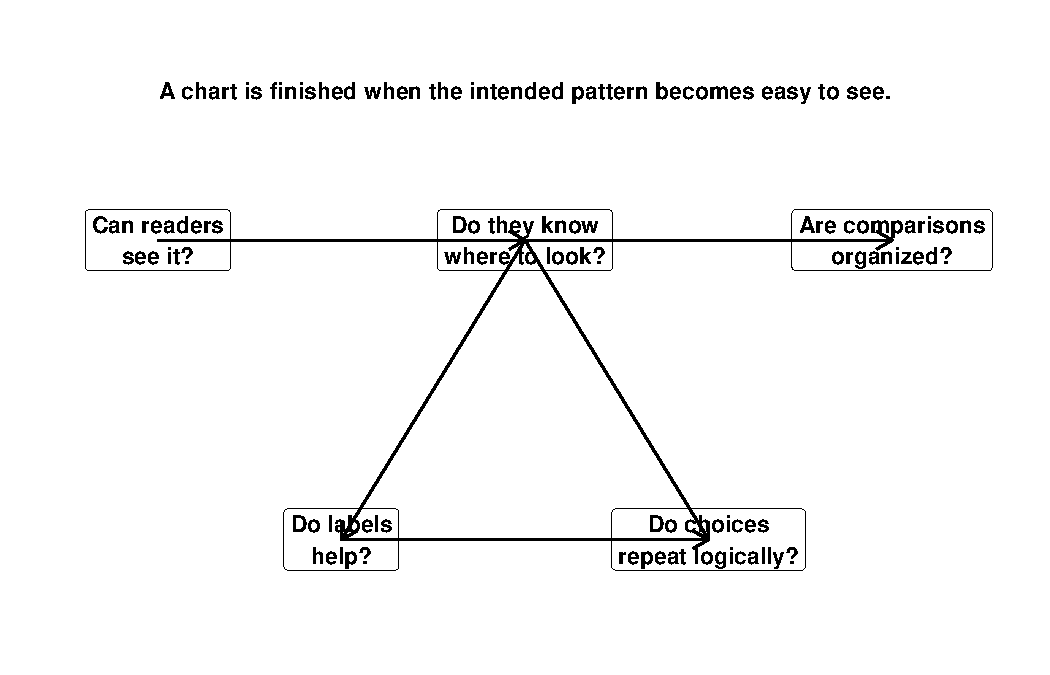
\includegraphics[width=0.9\linewidth,height=\textheight,keepaspectratio,alt={A framework diagram showing how clarity and control connect question, evidence, visual decision, and reader interpretation.}]{chapters/17-clarity-and-control_files/figure-pdf/fig-17-1-1.pdf}

}

\caption{\label{fig-17-1}The Clarity-Control Framework}

\end{figure}%

The code in Listing~\ref{lst-fig-17-1} produces Figure~\ref{fig-17-1}.

Figure 17.1 is not a theory to memorize. It is a working lens. When a
plot feels weak, Leo can ask which part of the framework is failing. If
the problem is visibility, he may need transparency, binning, or
zooming. If the problem is guidance, he may need better labels or
annotations. If the problem is structure, he may need ordering,
faceting, or a better layout.

\begin{tcolorbox}[enhanced jigsaw, arc=.35mm, bottomrule=.15mm, breakable, colback=white, colframe=quarto-callout-tip-color-frame, left=2mm, leftrule=.75mm, opacityback=0, rightrule=.15mm, toprule=.15mm]
\begin{minipage}[t]{5.5mm}
\textcolor{quarto-callout-tip-color}{\faLightbulb}
\end{minipage}%
\begin{minipage}[t]{\textwidth - 5.5mm}

\vspace{-3mm}\textbf{A practical rule}\vspace{3mm}

Do not refine everything at once. Fix the first reader problem first.
Then read the plot again. Visual control improves when each change has a
reason.

\end{minipage}%
\end{tcolorbox}

\section{Scales: Directing the Reader's
Eye}\label{scales-directing-the-readers-eye}

Scales connect data values to visual positions, colours, fills, sizes,
and labels. In Chapter 16, Leo met scales mostly as part of the
background machinery of \texttt{ggplot2}. In Chapter 17, scales become
one of his main instruments of control.

The most common scale controls for position are:

\begin{itemize}
\tightlist
\item
  \texttt{scale\_x\_*()} for the horizontal axis;
\item
  \texttt{scale\_y\_*()} for the vertical axis;
\item
  \texttt{breaks} to decide which values appear;
\item
  \texttt{labels} to decide how values are printed;
\item
  \texttt{limits} to restrict the displayed scale.
\end{itemize}

The star in \texttt{scale\_x\_*()} and \texttt{scale\_y\_*()} is not
literal code. It reminds Leo that the exact function depends on the kind
of variable. For continuous numeric axes, he might use
\texttt{scale\_x\_continuous()} or \texttt{scale\_y\_continuous()}. For
date axes, he might use \texttt{scale\_x\_date()}. For discrete
categories, he might use \texttt{scale\_x\_discrete()}.

The goal is not to control scales because the default is bad. The goal
is to control scales because readers should not have to decode avoidable
confusion.

\begin{codelisting}

\caption{\label{lst-fig-17-scale-default}Code for 17 scale default}

\centering{

\begin{Shaded}
\begin{Highlighting}[]
\NormalTok{score\_by\_country }\OtherTok{\textless{}{-}}\NormalTok{ df\_analysis }\SpecialCharTok{|\textgreater{}}
  \FunctionTok{filter}\NormalTok{(}\SpecialCharTok{!}\FunctionTok{is.na}\NormalTok{(country), }\SpecialCharTok{!}\FunctionTok{is.na}\NormalTok{(project\_score)) }\SpecialCharTok{|\textgreater{}}
  \FunctionTok{group\_by}\NormalTok{(country) }\SpecialCharTok{|\textgreater{}}
  \FunctionTok{summarise}\NormalTok{(}
    \AttributeTok{mean\_project\_score =} \FunctionTok{mean}\NormalTok{(project\_score, }\AttributeTok{na.rm =} \ConstantTok{TRUE}\NormalTok{),}
    \AttributeTok{learners =} \FunctionTok{n}\NormalTok{(),}
    \AttributeTok{.groups =} \StringTok{"drop"}
\NormalTok{  ) }\SpecialCharTok{|\textgreater{}}
  \FunctionTok{arrange}\NormalTok{(mean\_project\_score)}

\FunctionTok{ggplot}\NormalTok{(score\_by\_country, }\FunctionTok{aes}\NormalTok{(}\AttributeTok{x =}\NormalTok{ country, }\AttributeTok{y =}\NormalTok{ mean\_project\_score)) }\SpecialCharTok{+}
  \FunctionTok{geom\_col}\NormalTok{() }\SpecialCharTok{+}
  \FunctionTok{labs}\NormalTok{(}
    \AttributeTok{title =} \StringTok{"Average project score by country"}\NormalTok{,}
    \AttributeTok{x =} \StringTok{"Country"}\NormalTok{,}
    \AttributeTok{y =} \StringTok{"Average project score"}
\NormalTok{  )}
\end{Highlighting}
\end{Shaded}

}

\end{codelisting}%

\begin{figure}[H]

\centering{

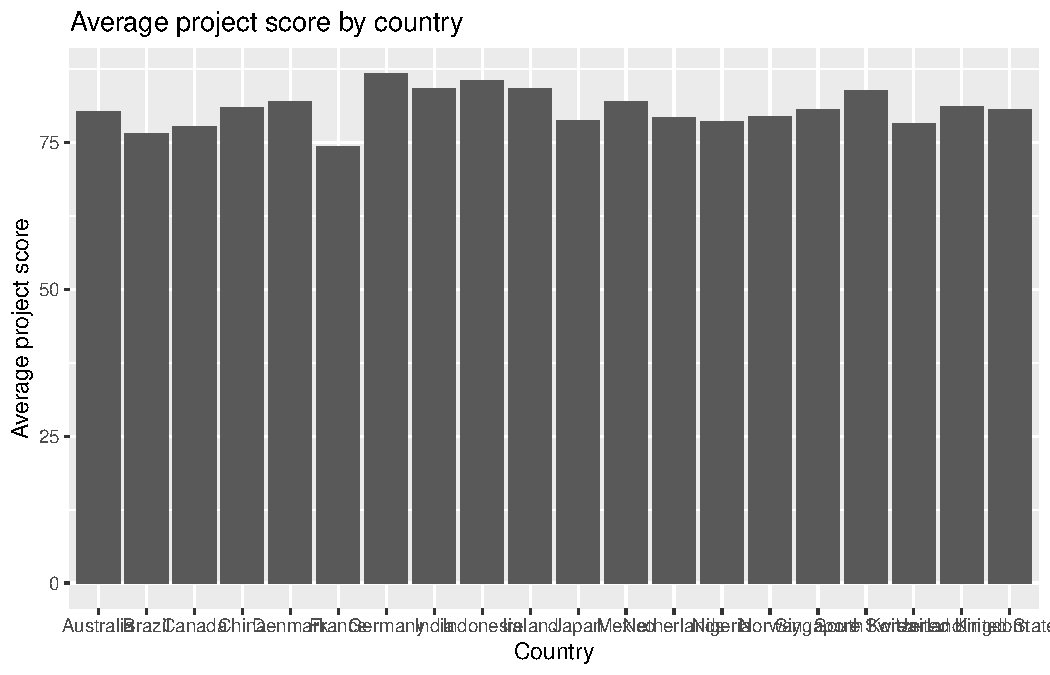
\includegraphics[width=0.9\linewidth,height=\textheight,keepaspectratio,alt={A default bar chart where the scale and ordering are correct but not optimised for easy comparison.}]{chapters/17-clarity-and-control_files/figure-pdf/fig-17-scale-default-1.pdf}

}

\caption{\label{fig-17-scale-default}A Default Scale Can Be Correct but
Harder to Read}

\end{figure}%

The code in Listing~\ref{lst-fig-17-scale-default} produces
Figure~\ref{fig-17-scale-default}.

Figure 17.2 is not wrong. It shows countries and average project scores.
But the reader may work harder than necessary. The country labels may be
cramped. The order may not guide comparison. The y-axis may show more
precision than the question needs.

A refined version controls the reading path.

\begin{codelisting}

\caption{\label{lst-fig-17-scale-improved}Code for 17 scale improved}

\centering{

\begin{Shaded}
\begin{Highlighting}[]
\NormalTok{score\_by\_country }\OtherTok{\textless{}{-}}\NormalTok{ score\_by\_country }\SpecialCharTok{|\textgreater{}}
  \FunctionTok{mutate}\NormalTok{(}\AttributeTok{country =} \FunctionTok{reorder}\NormalTok{(country, mean\_project\_score))}

\FunctionTok{ggplot}\NormalTok{(score\_by\_country, }\FunctionTok{aes}\NormalTok{(}\AttributeTok{x =}\NormalTok{ country, }\AttributeTok{y =}\NormalTok{ mean\_project\_score)) }\SpecialCharTok{+}
  \FunctionTok{geom\_col}\NormalTok{() }\SpecialCharTok{+}
  \FunctionTok{coord\_flip}\NormalTok{() }\SpecialCharTok{+}
  \FunctionTok{scale\_y\_continuous}\NormalTok{(}
    \AttributeTok{limits =} \FunctionTok{c}\NormalTok{(}\DecValTok{0}\NormalTok{, }\DecValTok{100}\NormalTok{),}
    \AttributeTok{breaks =} \FunctionTok{seq}\NormalTok{(}\DecValTok{0}\NormalTok{, }\DecValTok{100}\NormalTok{, }\AttributeTok{by =} \DecValTok{20}\NormalTok{),}
    \AttributeTok{labels =} \ControlFlowTok{function}\NormalTok{(x) }\FunctionTok{paste0}\NormalTok{(x, }\StringTok{"\%"}\NormalTok{)}
\NormalTok{  ) }\SpecialCharTok{+}
  \FunctionTok{labs}\NormalTok{(}
    \AttributeTok{title =} \StringTok{"Average project scores are easier to compare when the scale is controlled"}\NormalTok{,}
    \AttributeTok{subtitle =} \StringTok{"Countries are ordered by mean project score rather than alphabetically."}\NormalTok{,}
    \AttributeTok{x =} \ConstantTok{NULL}\NormalTok{,}
    \AttributeTok{y =} \StringTok{"Average project score"}\NormalTok{,}
    \AttributeTok{caption =} \StringTok{"Source: df\_analysis. Scores are shown on a 0 to 100 scale."}
\NormalTok{  ) }\SpecialCharTok{+}
\NormalTok{  chapter17\_theme}
\end{Highlighting}
\end{Shaded}

}

\end{codelisting}%

\begin{figure}[H]

\centering{

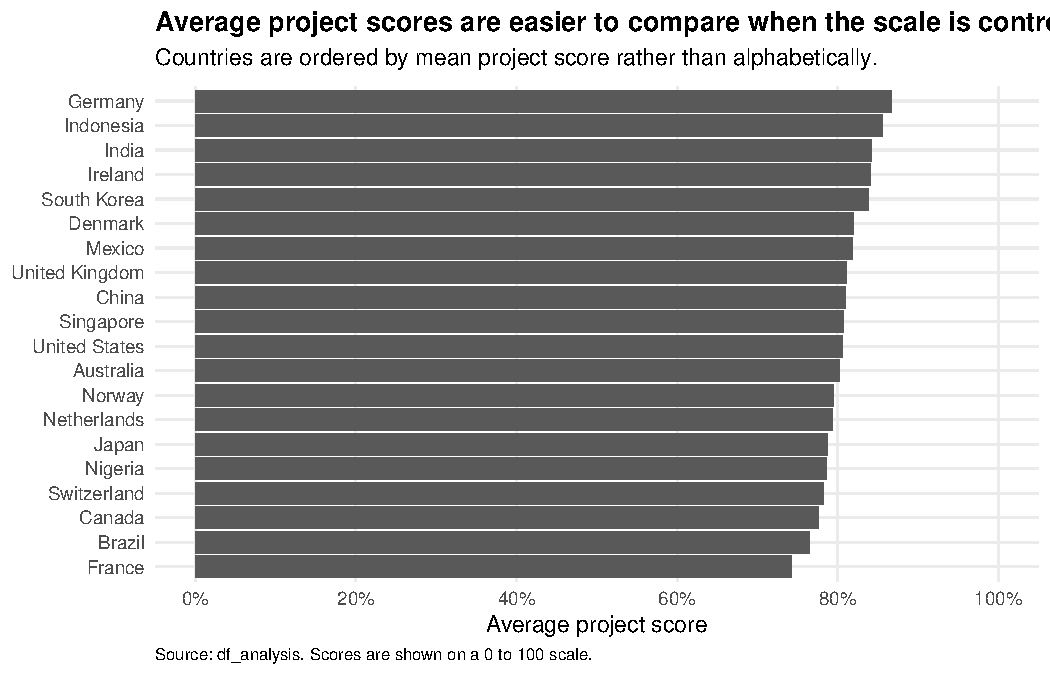
\includegraphics[width=0.9\linewidth,height=\textheight,keepaspectratio,alt={An improved bar chart with controlled scales and ordering that make the comparison easier to read.}]{chapters/17-clarity-and-control_files/figure-pdf/fig-17-scale-improved-1.pdf}

}

\caption{\label{fig-17-scale-improved}Controlled Scales and Ordering
Make the Comparison Easier to Read}

\end{figure}%

The code in Listing~\ref{lst-fig-17-scale-improved} produces
Figure~\ref{fig-17-scale-improved}.

Figure 17.3 does not change the underlying summaries. It changes the
reader's access to them. Ordering, axis breaks, labels, and orientation
help the comparison become visible.

\begin{tcolorbox}[enhanced jigsaw, arc=.35mm, bottomrule=.15mm, breakable, colback=white, colframe=quarto-callout-warning-color-frame, left=2mm, leftrule=.75mm, opacityback=0, rightrule=.15mm, toprule=.15mm]
\begin{minipage}[t]{5.5mm}
\textcolor{quarto-callout-warning-color}{\faExclamationTriangle}
\end{minipage}%
\begin{minipage}[t]{\textwidth - 5.5mm}

\vspace{-3mm}\textbf{Be careful with scale limits}\vspace{3mm}

Scale limits can remove data from the plot before the statistical layer
is calculated. When Leo wants to zoom into a region without dropping
observations, \texttt{coord\_cartesian()} is usually safer. This
distinction becomes important later in the chapter.

\end{minipage}%
\end{tcolorbox}

\section{Colour as Information}\label{colour-as-information}

Colour is powerful because the eye notices it quickly. That is also why
colour can become dangerous. If colour is used without purpose, it
creates noise. If too many colours appear at once, the reader starts
decoding the palette instead of reading the pattern.

A professional plot uses colour to carry meaning. It may distinguish
groups, show intensity, mark a warning, or highlight one comparison. It
should not be added merely because a plot looks plain.

In \texttt{ggplot2}, colour and fill are related but not identical:

\begin{itemize}
\tightlist
\item
  \texttt{colour} usually controls lines, points, and outlines;
\item
  \texttt{fill} usually controls the inside of bars, boxes, areas, and
  shapes that have an interior.
\end{itemize}

Useful scale functions include:

\begin{itemize}
\tightlist
\item
  \texttt{scale\_colour\_manual()} and \texttt{scale\_fill\_manual()}
  when Leo wants exact colours for exact categories;
\item
  \texttt{scale\_colour\_brewer()} and \texttt{scale\_fill\_brewer()}
  when he wants a named palette from ColorBrewer-style options;
\item
  \texttt{scale\_colour\_viridis\_d()} and
  \texttt{scale\_fill\_viridis\_d()} when he wants a discrete palette
  designed for perceptual clarity and accessibility;
\item
  \texttt{scale\_colour\_viridis\_c()} and
  \texttt{scale\_fill\_viridis\_c()} when he is mapping continuous
  values.
\end{itemize}

Viridis palettes are often a good default when the plot needs a colour
scale that remains readable across different displays and is friendlier
to readers with common forms of colour-vision deficiency. The point is
not that viridis is always beautiful. The point is that it is
dependable.

\begin{codelisting}

\caption{\label{lst-fig-17-colour-palettes}Code for 17 colour palettes}

\centering{

\begin{Shaded}
\begin{Highlighting}[]
\NormalTok{palette\_data }\OtherTok{\textless{}{-}}\NormalTok{ df\_analysis }\SpecialCharTok{|\textgreater{}}
  \FunctionTok{filter}\NormalTok{(}\SpecialCharTok{!}\FunctionTok{is.na}\NormalTok{(study\_band), }\SpecialCharTok{!}\FunctionTok{is.na}\NormalTok{(completion\_status), }\SpecialCharTok{!}\FunctionTok{is.na}\NormalTok{(project\_score)) }\SpecialCharTok{|\textgreater{}}
  \FunctionTok{group\_by}\NormalTok{(study\_band, completion\_status) }\SpecialCharTok{|\textgreater{}}
  \FunctionTok{summarise}\NormalTok{(}\AttributeTok{mean\_project\_score =} \FunctionTok{mean}\NormalTok{(project\_score, }\AttributeTok{na.rm =} \ConstantTok{TRUE}\NormalTok{), }\AttributeTok{.groups =} \StringTok{"drop"}\NormalTok{)}

\FunctionTok{ggplot}\NormalTok{(palette\_data, }\FunctionTok{aes}\NormalTok{(}\AttributeTok{x =}\NormalTok{ study\_band, }\AttributeTok{y =}\NormalTok{ mean\_project\_score, }\AttributeTok{fill =}\NormalTok{ completion\_status)) }\SpecialCharTok{+}
  \FunctionTok{geom\_col}\NormalTok{(}\AttributeTok{position =} \StringTok{"dodge"}\NormalTok{) }\SpecialCharTok{+}
  \FunctionTok{scale\_fill\_viridis\_d}\NormalTok{(}\AttributeTok{option =} \StringTok{"D"}\NormalTok{, }\AttributeTok{end =} \FloatTok{0.85}\NormalTok{) }\SpecialCharTok{+}
  \FunctionTok{scale\_y\_continuous}\NormalTok{(}\AttributeTok{limits =} \FunctionTok{c}\NormalTok{(}\DecValTok{0}\NormalTok{, }\DecValTok{100}\NormalTok{), }\AttributeTok{breaks =} \FunctionTok{seq}\NormalTok{(}\DecValTok{0}\NormalTok{, }\DecValTok{100}\NormalTok{, }\DecValTok{20}\NormalTok{)) }\SpecialCharTok{+}
  \FunctionTok{labs}\NormalTok{(}
    \AttributeTok{title =} \StringTok{"Colour should separate meaning, not decorate the chart"}\NormalTok{,}
    \AttributeTok{subtitle =} \StringTok{"Here fill colour distinguishes completion status across study bands."}\NormalTok{,}
    \AttributeTok{x =} \ConstantTok{NULL}\NormalTok{,}
    \AttributeTok{y =} \StringTok{"Average project score"}\NormalTok{,}
    \AttributeTok{fill =} \StringTok{"Completion status"}\NormalTok{,}
    \AttributeTok{caption =} \StringTok{"Figure uses scale\_fill\_viridis\_d() for an accessible discrete palette."}
\NormalTok{  ) }\SpecialCharTok{+}
\NormalTok{  chapter17\_theme }\SpecialCharTok{+}
  \FunctionTok{theme}\NormalTok{(}\AttributeTok{axis.text.x =} \FunctionTok{element\_text}\NormalTok{(}\AttributeTok{angle =} \DecValTok{20}\NormalTok{, }\AttributeTok{hjust =} \DecValTok{1}\NormalTok{))}
\end{Highlighting}
\end{Shaded}

}

\end{codelisting}%

\begin{figure}[H]

\centering{

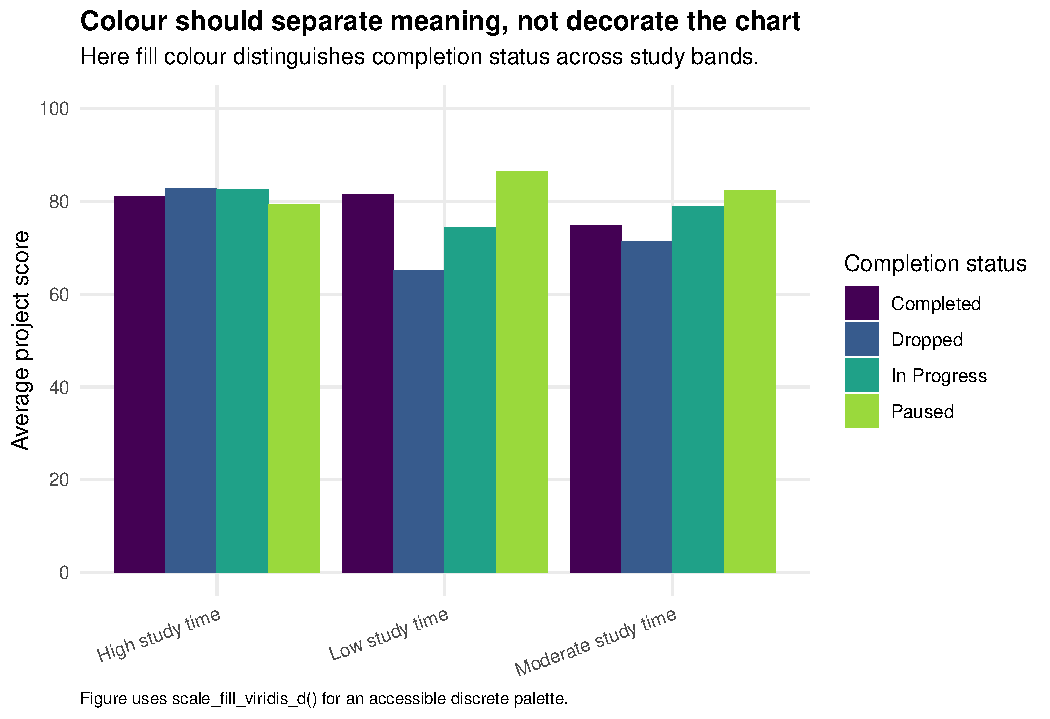
\includegraphics[width=0.9\linewidth,height=\textheight,keepaspectratio,alt={A comparison of colour palette choices showing how colour can support or distract from interpretation.}]{chapters/17-clarity-and-control_files/figure-pdf/fig-17-colour-palettes-1.pdf}

}

\caption{\label{fig-17-colour-palettes}Comparison of Colour Palette
Choices}

\end{figure}%

The code in Listing~\ref{lst-fig-17-colour-palettes} produces
Figure~\ref{fig-17-colour-palettes}.

Figure 17.4 uses colour to distinguish completion status. Colour is not
doing everything. Position, grouping, title, subtitle, axis labels, and
legend also contribute to clarity.

\begin{tcolorbox}[enhanced jigsaw, arc=.35mm, bottomrule=.15mm, breakable, colback=white, colframe=quarto-callout-important-color-frame, left=2mm, leftrule=.75mm, opacityback=0, rightrule=.15mm, toprule=.15mm]
\begin{minipage}[t]{5.5mm}
\textcolor{quarto-callout-important-color}{\faExclamation}
\end{minipage}%
\begin{minipage}[t]{\textwidth - 5.5mm}

\vspace{-3mm}\textbf{Colour rule}\vspace{3mm}

Before adding colour, Leo should complete this sentence: ``Colour is
used here to show \_\_\_\_\_\_\_\_.'' If the sentence has no clear
answer, the plot probably does not need colour.

\end{minipage}%
\end{tcolorbox}

\section{Themes: Taking Control of
Appearance}\label{themes-taking-control-of-appearance}

A theme controls the non-data parts of a plot: background, gridlines,
text, legend placement, panel spacing, axis ticks, and more. Themes
matter because visual noise often comes from non-data elements.

The theme is not the evidence. It is the room in which the evidence is
placed.

\texttt{ggplot2} includes several ready-made themes. The most common are
not better or worse in general. They are useful in different situations.

\begin{codelisting}

\caption{\label{lst-tbl-17-2}Code for 17 2}

\centering{

\begin{Shaded}
\begin{Highlighting}[]
\NormalTok{theme\_table }\OtherTok{\textless{}{-}}\NormalTok{ tibble}\SpecialCharTok{::}\FunctionTok{tribble}\NormalTok{(}
  \SpecialCharTok{\textasciitilde{}}\NormalTok{Theme, }\SpecialCharTok{\textasciitilde{}}\StringTok{\textasciigrave{}}\AttributeTok{Best used when}\StringTok{\textasciigrave{}}\NormalTok{, }\SpecialCharTok{\textasciitilde{}}\NormalTok{Strength, }\SpecialCharTok{\textasciitilde{}}\NormalTok{Caution,}
  \StringTok{"theme\_minimal()"}\NormalTok{, }\StringTok{"You want a clean analytical chart with light visual structure"}\NormalTok{, }\StringTok{"Reduces clutter while keeping grid guidance"}\NormalTok{, }\StringTok{"Can look too plain if labels and hierarchy are weak"}\NormalTok{,}
  \StringTok{"theme\_classic()"}\NormalTok{, }\StringTok{"You want a traditional publication{-}style plot"}\NormalTok{, }\StringTok{"Strong axes and low background noise"}\NormalTok{, }\StringTok{"Gridlines are absent, so comparisons may be harder in some plots"}\NormalTok{,}
  \StringTok{"theme\_void()"}\NormalTok{, }\StringTok{"You want maps, diagrams, or plots where axes are irrelevant"}\NormalTok{, }\StringTok{"Removes nearly all non{-}data elements"}\NormalTok{, }\StringTok{"Dangerous for ordinary analytical charts that need scales"}\NormalTok{,}
  \StringTok{"theme\_bw()"}\NormalTok{, }\StringTok{"You want a clear white{-}background plot with visible panel structure"}\NormalTok{, }\StringTok{"Works well in print and reports"}\NormalTok{, }\StringTok{"Can feel heavier than necessary for simple plots"}\NormalTok{,}
  \StringTok{"theme\_light()"}\NormalTok{, }\StringTok{"You want a gentle grid and light background"}\NormalTok{, }\StringTok{"Readable for exploratory plots"}\NormalTok{, }\StringTok{"May still need text and legend refinement"}
\NormalTok{)}

\NormalTok{knitr}\SpecialCharTok{::}\FunctionTok{kable}\NormalTok{(theme\_table)}
\end{Highlighting}
\end{Shaded}

}

\end{codelisting}%

{

\begin{longtable}[]{@{}
  >{\raggedright\arraybackslash}p{(\linewidth - 6\tabcolsep) * \real{0.0829}}
  >{\raggedright\arraybackslash}p{(\linewidth - 6\tabcolsep) * \real{0.3523}}
  >{\raggedright\arraybackslash}p{(\linewidth - 6\tabcolsep) * \real{0.2280}}
  >{\raggedright\arraybackslash}p{(\linewidth - 6\tabcolsep) * \real{0.3368}}@{}}

\caption{\label{tbl-17-2}Comparison of Common ggplot2 Themes}

\tabularnewline

\toprule\noalign{}
\begin{minipage}[b]{\linewidth}\raggedright
Theme
\end{minipage} & \begin{minipage}[b]{\linewidth}\raggedright
Best used when
\end{minipage} & \begin{minipage}[b]{\linewidth}\raggedright
Strength
\end{minipage} & \begin{minipage}[b]{\linewidth}\raggedright
Caution
\end{minipage} \\
\midrule\noalign{}
\endhead
\bottomrule\noalign{}
\endlastfoot
theme\_minimal() & You want a clean analytical chart with light visual
structure & Reduces clutter while keeping grid guidance & Can look too
plain if labels and hierarchy are weak \\
theme\_classic() & You want a traditional publication-style plot &
Strong axes and low background noise & Gridlines are absent, so
comparisons may be harder in some plots \\
theme\_void() & You want maps, diagrams, or plots where axes are
irrelevant & Removes nearly all non-data elements & Dangerous for
ordinary analytical charts that need scales \\
theme\_bw() & You want a clear white-background plot with visible panel
structure & Works well in print and reports & Can feel heavier than
necessary for simple plots \\
theme\_light() & You want a gentle grid and light background & Readable
for exploratory plots & May still need text and legend refinement \\

\end{longtable}

}

The code in Listing~\ref{lst-tbl-17-2} produces Table~\ref{tbl-17-2}.

Table 17.2 gives Leo a practical comparison. The larger lesson is
simple: a theme is a starting point, not a substitute for design
judgment.

The most useful theme function is often \texttt{theme()} itself, because
it lets Leo control specific parts of the plot.

\begin{codelisting}

\caption{\label{lst-fig-17-theme-control}Code for 17 theme control}

\centering{

\begin{Shaded}
\begin{Highlighting}[]
\FunctionTok{ggplot}\NormalTok{(score\_by\_country, }\FunctionTok{aes}\NormalTok{(}\AttributeTok{x =}\NormalTok{ country, }\AttributeTok{y =}\NormalTok{ mean\_project\_score)) }\SpecialCharTok{+}
  \FunctionTok{geom\_col}\NormalTok{() }\SpecialCharTok{+}
  \FunctionTok{coord\_flip}\NormalTok{() }\SpecialCharTok{+}
  \FunctionTok{scale\_y\_continuous}\NormalTok{(}\AttributeTok{limits =} \FunctionTok{c}\NormalTok{(}\DecValTok{0}\NormalTok{, }\DecValTok{100}\NormalTok{), }\AttributeTok{breaks =} \FunctionTok{seq}\NormalTok{(}\DecValTok{0}\NormalTok{, }\DecValTok{100}\NormalTok{, }\DecValTok{20}\NormalTok{)) }\SpecialCharTok{+}
  \FunctionTok{labs}\NormalTok{(}
    \AttributeTok{title =} \StringTok{"Theme control helps the reader focus on the comparison"}\NormalTok{,}
    \AttributeTok{subtitle =} \StringTok{"The background is reduced, the title is emphasized, and minor gridlines are removed."}\NormalTok{,}
    \AttributeTok{x =} \ConstantTok{NULL}\NormalTok{,}
    \AttributeTok{y =} \StringTok{"Average project score"}
\NormalTok{  ) }\SpecialCharTok{+}
  \FunctionTok{theme\_minimal}\NormalTok{(}\AttributeTok{base\_size =} \DecValTok{11}\NormalTok{) }\SpecialCharTok{+}
  \FunctionTok{theme}\NormalTok{(}
    \AttributeTok{plot.title =} \FunctionTok{element\_text}\NormalTok{(}\AttributeTok{face =} \StringTok{"bold"}\NormalTok{, }\AttributeTok{size =} \DecValTok{13}\NormalTok{),}
    \AttributeTok{plot.subtitle =} \FunctionTok{element\_text}\NormalTok{(}\AttributeTok{size =} \DecValTok{10}\NormalTok{, }\AttributeTok{margin =} \FunctionTok{margin}\NormalTok{(}\AttributeTok{b =} \DecValTok{8}\NormalTok{)),}
    \AttributeTok{panel.grid.minor =} \FunctionTok{element\_blank}\NormalTok{(),}
    \AttributeTok{panel.grid.major.y =} \FunctionTok{element\_blank}\NormalTok{()}
\NormalTok{  )}
\end{Highlighting}
\end{Shaded}

}

\end{codelisting}%

\begin{figure}[H]

\centering{

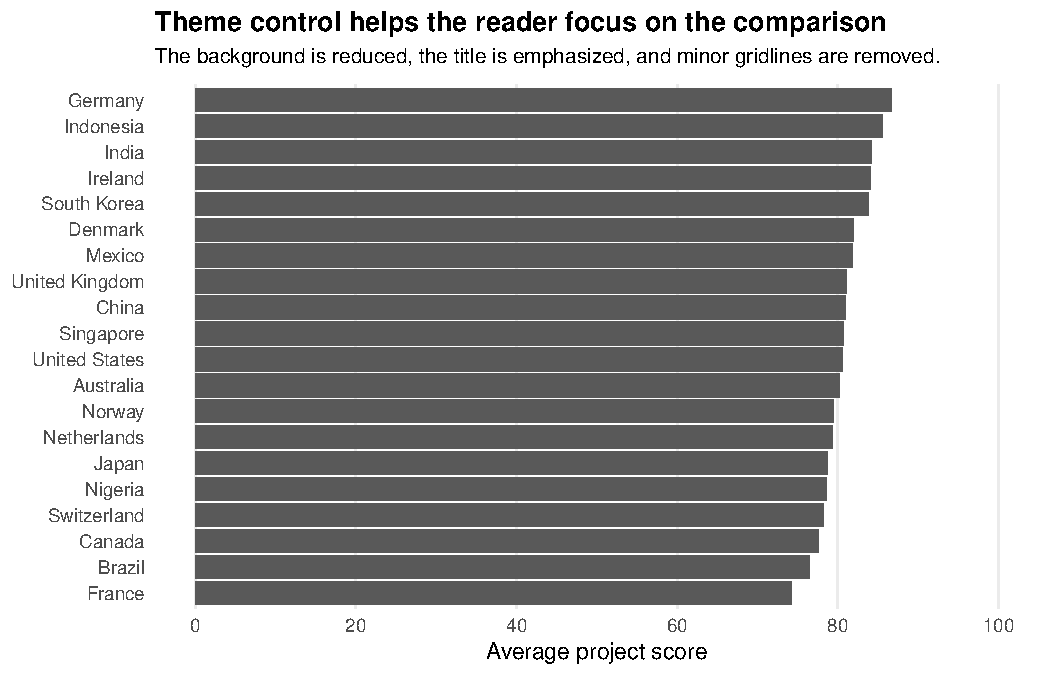
\includegraphics[width=0.9\linewidth,height=\textheight,keepaspectratio,alt={A plot demonstrating how theme settings control non-data elements such as gridlines, text, and background.}]{chapters/17-clarity-and-control_files/figure-pdf/fig-17-theme-control-1.pdf}

}

\caption{\label{fig-17-theme-control}theme() Gives Direct Control Over
Non-Data Elements}

\end{figure}%

The code in Listing~\ref{lst-fig-17-theme-control} produces
Figure~\ref{fig-17-theme-control}.

Figure 17.5 shows a disciplined use of \texttt{theme()}. Leo is not
changing the plot because he wants variety. He is changing the plot
because each non-data element either helps or distracts.

\section{Controlling Text}\label{controlling-text}

Text is one of the most neglected parts of beginner plots. Many learners
spend energy choosing colours and geoms but leave the title vague, the
subtitle absent, the axis labels mechanical, and the caption unused.

That is a mistake. Text is not decoration. Text guides interpretation.

The most important text controls are:

\begin{itemize}
\tightlist
\item
  \texttt{labs()} for title, subtitle, caption, axes, and legend titles;
\item
  \texttt{element\_text()} inside \texttt{theme()} for size, face,
  colour, angle, and alignment;
\item
  \texttt{annotate()} for direct notes inside the plotting area;
\item
  \texttt{geom\_text()} or \texttt{geom\_label()} for labels attached to
  data;
\item
  \texttt{ggrepel} when labels may collide;
\item
  \texttt{ggtext} when markdown or HTML styling is needed.
\end{itemize}

A plain title says what the plot is. A useful title says what comparison
the reader should examine.

\begin{codelisting}

\caption{\label{lst-fig-17-text-control}Code for 17 text control}

\centering{

\begin{Shaded}
\begin{Highlighting}[]
\NormalTok{weekly\_scores }\OtherTok{\textless{}{-}}\NormalTok{ df\_analysis }\SpecialCharTok{|\textgreater{}}
  \FunctionTok{filter}\NormalTok{(}\SpecialCharTok{!}\FunctionTok{is.na}\NormalTok{(week), }\SpecialCharTok{!}\FunctionTok{is.na}\NormalTok{(project\_score)) }\SpecialCharTok{|\textgreater{}}
  \FunctionTok{group\_by}\NormalTok{(week) }\SpecialCharTok{|\textgreater{}}
  \FunctionTok{summarise}\NormalTok{(}\AttributeTok{mean\_project\_score =} \FunctionTok{mean}\NormalTok{(project\_score, }\AttributeTok{na.rm =} \ConstantTok{TRUE}\NormalTok{), }\AttributeTok{.groups =} \StringTok{"drop"}\NormalTok{) }\SpecialCharTok{|\textgreater{}}
  \FunctionTok{arrange}\NormalTok{(week)}

\FunctionTok{ggplot}\NormalTok{(weekly\_scores, }\FunctionTok{aes}\NormalTok{(}\AttributeTok{x =}\NormalTok{ week, }\AttributeTok{y =}\NormalTok{ mean\_project\_score)) }\SpecialCharTok{+}
  \FunctionTok{geom\_line}\NormalTok{(}\AttributeTok{linewidth =} \FloatTok{0.8}\NormalTok{) }\SpecialCharTok{+}
  \FunctionTok{geom\_point}\NormalTok{(}\AttributeTok{size =} \DecValTok{2}\NormalTok{) }\SpecialCharTok{+}
  \FunctionTok{scale\_x\_continuous}\NormalTok{(}\AttributeTok{breaks =} \FunctionTok{sort}\NormalTok{(}\FunctionTok{unique}\NormalTok{(weekly\_scores}\SpecialCharTok{$}\NormalTok{week))) }\SpecialCharTok{+}
  \FunctionTok{scale\_y\_continuous}\NormalTok{(}\AttributeTok{limits =} \FunctionTok{c}\NormalTok{(}\DecValTok{0}\NormalTok{, }\DecValTok{100}\NormalTok{), }\AttributeTok{breaks =} \FunctionTok{seq}\NormalTok{(}\DecValTok{0}\NormalTok{, }\DecValTok{100}\NormalTok{, }\DecValTok{20}\NormalTok{)) }\SpecialCharTok{+}
  \FunctionTok{labs}\NormalTok{(}
    \AttributeTok{title =} \StringTok{"Project scores become easier to read when text gives direction"}\NormalTok{,}
    \AttributeTok{subtitle =} \StringTok{"The chart tracks average project score across learning weeks."}\NormalTok{,}
    \AttributeTok{x =} \StringTok{"Learning week"}\NormalTok{,}
    \AttributeTok{y =} \StringTok{"Average project score"}\NormalTok{,}
    \AttributeTok{caption =} \StringTok{"Source: df\_analysis. Weekly values are group means."}
\NormalTok{  ) }\SpecialCharTok{+}
\NormalTok{  chapter17\_theme }\SpecialCharTok{+}
  \FunctionTok{theme}\NormalTok{(}
    \AttributeTok{plot.title =} \FunctionTok{element\_text}\NormalTok{(}\AttributeTok{size =} \DecValTok{13}\NormalTok{, }\AttributeTok{face =} \StringTok{"bold"}\NormalTok{),}
    \AttributeTok{axis.title.x =} \FunctionTok{element\_text}\NormalTok{(}\AttributeTok{margin =} \FunctionTok{margin}\NormalTok{(}\AttributeTok{t =} \DecValTok{8}\NormalTok{)),}
    \AttributeTok{axis.title.y =} \FunctionTok{element\_text}\NormalTok{(}\AttributeTok{margin =} \FunctionTok{margin}\NormalTok{(}\AttributeTok{r =} \DecValTok{8}\NormalTok{))}
\NormalTok{  )}
\end{Highlighting}
\end{Shaded}

}

\end{codelisting}%

\begin{figure}[H]

\centering{

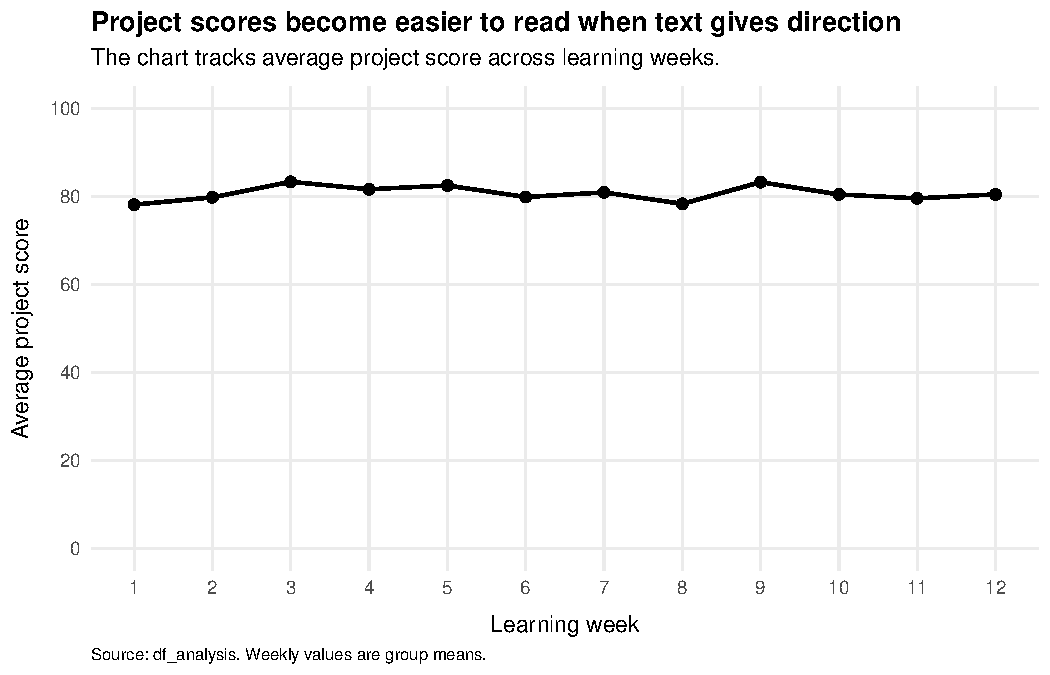
\includegraphics[width=0.9\linewidth,height=\textheight,keepaspectratio,alt={A plot showing how title, subtitle, axis labels, and caption guide reader interpretation.}]{chapters/17-clarity-and-control_files/figure-pdf/fig-17-text-control-1.pdf}

}

\caption{\label{fig-17-text-control}Text Control Turns a Plot from
Output into Guidance}

\end{figure}%

The code in Listing~\ref{lst-fig-17-text-control} produces
Figure~\ref{fig-17-text-control}.

Figure 17.6 demonstrates an important shift. The plot does not merely
announce a variable. It tells the reader what kind of movement to
inspect.

\begin{tcolorbox}[enhanced jigsaw, arc=.35mm, bottomrule=.15mm, breakable, colback=white, colframe=quarto-callout-tip-color-frame, left=2mm, leftrule=.75mm, opacityback=0, rightrule=.15mm, toprule=.15mm]
\begin{minipage}[t]{5.5mm}
\textcolor{quarto-callout-tip-color}{\faLightbulb}
\end{minipage}%
\begin{minipage}[t]{\textwidth - 5.5mm}

\vspace{-3mm}\textbf{Text test}\vspace{3mm}

After writing a title, Leo should ask: could this title fit almost any
plot? If yes, it is probably too generic. A useful title belongs to this
plot.

\end{minipage}%
\end{tcolorbox}

\section{Controlling Backgrounds, Borders and
Gridlines}\label{controlling-backgrounds-borders-and-gridlines}

Gridlines, backgrounds, and borders are controlled with theme elements:

\begin{itemize}
\tightlist
\item
  \texttt{element\_rect()} controls rectangular areas such as plot
  backgrounds, panel backgrounds, and legend boxes;
\item
  \texttt{element\_line()} controls lines such as gridlines, axis lines,
  and ticks;
\item
  \texttt{element\_blank()} removes an element completely.
\end{itemize}

These controls matter because the eye has limited attention. Heavy
gridlines, dark backgrounds, thick borders, and unnecessary ticks can
compete with the data.

\begin{codelisting}

\caption{\label{lst-fig-17-lines-rectangles}Code for 17 lines
rectangles}

\centering{

\begin{Shaded}
\begin{Highlighting}[]
\FunctionTok{ggplot}\NormalTok{(weekly\_scores, }\FunctionTok{aes}\NormalTok{(}\AttributeTok{x =}\NormalTok{ week, }\AttributeTok{y =}\NormalTok{ mean\_project\_score)) }\SpecialCharTok{+}
  \FunctionTok{geom\_line}\NormalTok{(}\AttributeTok{linewidth =} \FloatTok{0.8}\NormalTok{) }\SpecialCharTok{+}
  \FunctionTok{geom\_point}\NormalTok{(}\AttributeTok{size =} \DecValTok{2}\NormalTok{) }\SpecialCharTok{+}
  \FunctionTok{scale\_x\_continuous}\NormalTok{(}\AttributeTok{breaks =} \FunctionTok{sort}\NormalTok{(}\FunctionTok{unique}\NormalTok{(weekly\_scores}\SpecialCharTok{$}\NormalTok{week))) }\SpecialCharTok{+}
  \FunctionTok{scale\_y\_continuous}\NormalTok{(}\AttributeTok{limits =} \FunctionTok{c}\NormalTok{(}\DecValTok{0}\NormalTok{, }\DecValTok{100}\NormalTok{), }\AttributeTok{breaks =} \FunctionTok{seq}\NormalTok{(}\DecValTok{0}\NormalTok{, }\DecValTok{100}\NormalTok{, }\DecValTok{20}\NormalTok{)) }\SpecialCharTok{+}
  \FunctionTok{labs}\NormalTok{(}
    \AttributeTok{title =} \StringTok{"Gridlines should support reading, not compete with the data"}\NormalTok{,}
    \AttributeTok{x =} \StringTok{"Learning week"}\NormalTok{,}
    \AttributeTok{y =} \StringTok{"Average project score"}
\NormalTok{  ) }\SpecialCharTok{+}
  \FunctionTok{theme\_minimal}\NormalTok{(}\AttributeTok{base\_size =} \DecValTok{11}\NormalTok{) }\SpecialCharTok{+}
  \FunctionTok{theme}\NormalTok{(}
    \AttributeTok{panel.background =} \FunctionTok{element\_rect}\NormalTok{(}\AttributeTok{fill =} \StringTok{"white"}\NormalTok{, }\AttributeTok{colour =} \ConstantTok{NA}\NormalTok{),}
    \AttributeTok{plot.background =} \FunctionTok{element\_rect}\NormalTok{(}\AttributeTok{fill =} \StringTok{"white"}\NormalTok{, }\AttributeTok{colour =} \ConstantTok{NA}\NormalTok{),}
    \AttributeTok{panel.grid.minor =} \FunctionTok{element\_blank}\NormalTok{(),}
    \AttributeTok{panel.grid.major.x =} \FunctionTok{element\_blank}\NormalTok{(),}
    \AttributeTok{panel.grid.major.y =} \FunctionTok{element\_line}\NormalTok{(}\AttributeTok{linewidth =} \FloatTok{0.25}\NormalTok{),}
    \AttributeTok{axis.ticks.x =} \FunctionTok{element\_line}\NormalTok{(}\AttributeTok{linewidth =} \FloatTok{0.25}\NormalTok{)}
\NormalTok{  )}
\end{Highlighting}
\end{Shaded}

}

\end{codelisting}%

\begin{figure}[H]

\centering{

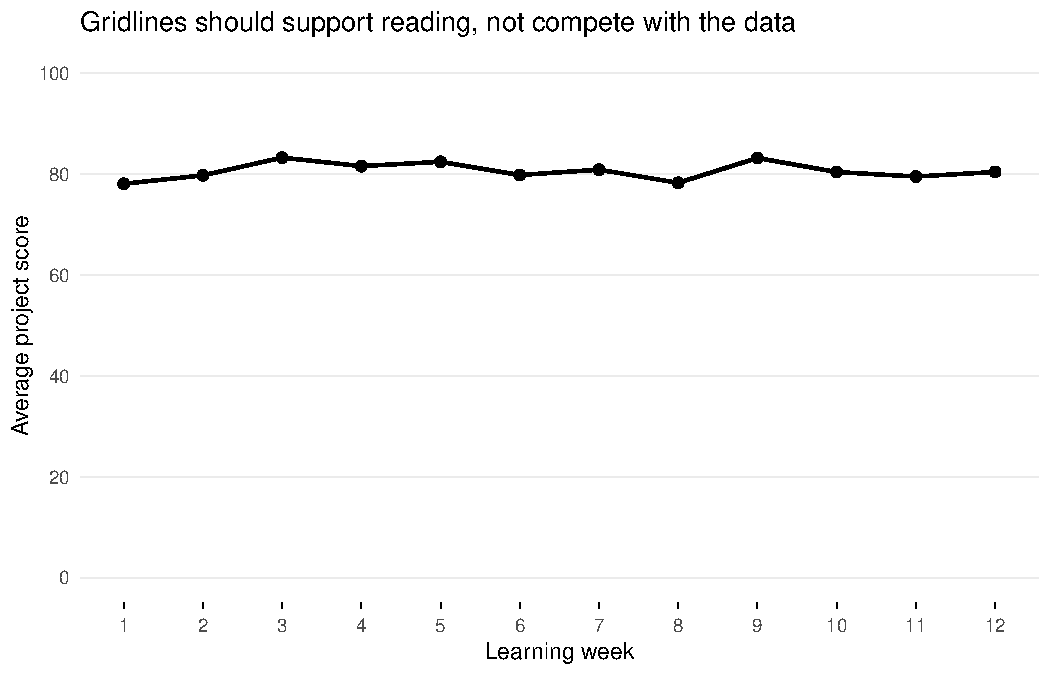
\includegraphics[width=0.9\linewidth,height=\textheight,keepaspectratio,alt={A plot demonstrating how rectangular and line elements can either reduce clutter or add unnecessary visual noise.}]{chapters/17-clarity-and-control_files/figure-pdf/fig-17-lines-rectangles-1.pdf}

}

\caption{\label{fig-17-lines-rectangles}Rectangular and Line Elements
Can Reduce or Increase Visual Clutter}

\end{figure}%

The code in Listing~\ref{lst-fig-17-lines-rectangles} produces
Figure~\ref{fig-17-lines-rectangles}.

Figure 17.7 keeps only the gridlines that help the reader estimate
values. This is a quiet form of design. Nothing flashy happens, but the
chart becomes calmer.

\section{Legends That Help Instead of
Confuse}\label{legends-that-help-instead-of-confuse}

A legend is a guide. It should reduce the reader's work. If the reader
must constantly move from the plot to the legend and back again, the
legend may be doing too much.

Common legend controls include:

\begin{itemize}
\tightlist
\item
  \texttt{legend.position} to place the legend;
\item
  \texttt{legend.title} to control the legend title;
\item
  \texttt{legend.text} for legend labels;
\item
  \texttt{guides()} when Leo needs more specific legend control;
\item
  direct labels when a legend is unnecessary.
\end{itemize}

The first question is not, ``Where should the legend go?'' The first
question is, ``Does this plot need a legend at all?''

\begin{codelisting}

\caption{\label{lst-fig-17-legend-design}Code for 17 legend design}

\centering{

\begin{Shaded}
\begin{Highlighting}[]
\NormalTok{mode\_scores }\OtherTok{\textless{}{-}}\NormalTok{ df\_analysis }\SpecialCharTok{|\textgreater{}}
  \FunctionTok{filter}\NormalTok{(}\SpecialCharTok{!}\FunctionTok{is.na}\NormalTok{(preferred\_learning\_mode), }\SpecialCharTok{!}\FunctionTok{is.na}\NormalTok{(week), }\SpecialCharTok{!}\FunctionTok{is.na}\NormalTok{(project\_score)) }\SpecialCharTok{|\textgreater{}}
  \FunctionTok{group\_by}\NormalTok{(preferred\_learning\_mode, week) }\SpecialCharTok{|\textgreater{}}
  \FunctionTok{summarise}\NormalTok{(}\AttributeTok{mean\_project\_score =} \FunctionTok{mean}\NormalTok{(project\_score, }\AttributeTok{na.rm =} \ConstantTok{TRUE}\NormalTok{), }\AttributeTok{.groups =} \StringTok{"drop"}\NormalTok{)}

\FunctionTok{ggplot}\NormalTok{(mode\_scores, }\FunctionTok{aes}\NormalTok{(}\AttributeTok{x =}\NormalTok{ week, }\AttributeTok{y =}\NormalTok{ mean\_project\_score, }\AttributeTok{colour =}\NormalTok{ preferred\_learning\_mode)) }\SpecialCharTok{+}
  \FunctionTok{geom\_line}\NormalTok{(}\AttributeTok{linewidth =} \FloatTok{0.8}\NormalTok{) }\SpecialCharTok{+}
  \FunctionTok{geom\_point}\NormalTok{(}\AttributeTok{size =} \FloatTok{1.8}\NormalTok{) }\SpecialCharTok{+}
  \FunctionTok{scale\_x\_continuous}\NormalTok{(}\AttributeTok{breaks =} \FunctionTok{sort}\NormalTok{(}\FunctionTok{unique}\NormalTok{(mode\_scores}\SpecialCharTok{$}\NormalTok{week))) }\SpecialCharTok{+}
  \FunctionTok{scale\_y\_continuous}\NormalTok{(}\AttributeTok{limits =} \FunctionTok{c}\NormalTok{(}\DecValTok{0}\NormalTok{, }\DecValTok{100}\NormalTok{), }\AttributeTok{breaks =} \FunctionTok{seq}\NormalTok{(}\DecValTok{0}\NormalTok{, }\DecValTok{100}\NormalTok{, }\DecValTok{20}\NormalTok{)) }\SpecialCharTok{+}
  \FunctionTok{scale\_colour\_viridis\_d}\NormalTok{(}\AttributeTok{end =} \FloatTok{0.85}\NormalTok{) }\SpecialCharTok{+}
  \FunctionTok{labs}\NormalTok{(}
    \AttributeTok{title =} \StringTok{"A useful legend explains the mapping without interrupting the reading path"}\NormalTok{,}
    \AttributeTok{subtitle =} \StringTok{"Legend title and placement are part of the design, not an afterthought."}\NormalTok{,}
    \AttributeTok{x =} \StringTok{"Learning week"}\NormalTok{,}
    \AttributeTok{y =} \StringTok{"Average project score"}\NormalTok{,}
    \AttributeTok{colour =} \StringTok{"Learning mode"}
\NormalTok{  ) }\SpecialCharTok{+}
\NormalTok{  chapter17\_theme }\SpecialCharTok{+}
  \FunctionTok{theme}\NormalTok{(}
    \AttributeTok{legend.position =} \StringTok{"bottom"}\NormalTok{,}
    \AttributeTok{legend.title =} \FunctionTok{element\_text}\NormalTok{(}\AttributeTok{face =} \StringTok{"bold"}\NormalTok{)}
\NormalTok{  )}
\end{Highlighting}
\end{Shaded}

}

\end{codelisting}%

\begin{figure}[H]

\centering{

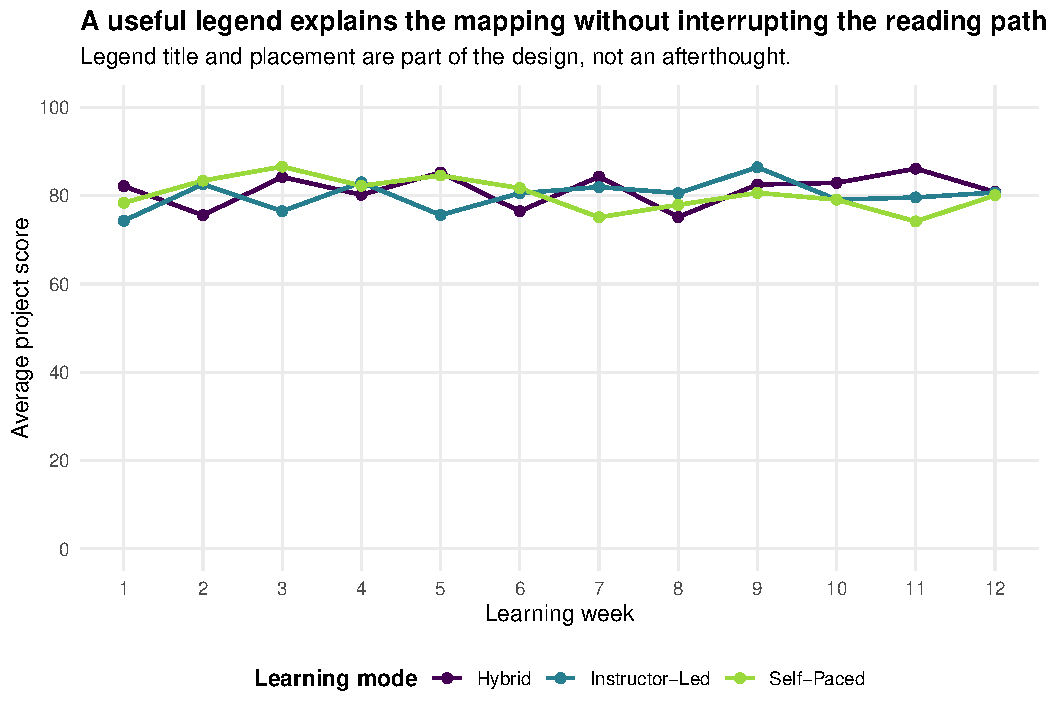
\includegraphics[width=0.9\linewidth,height=\textheight,keepaspectratio,alt={A comparison showing how a poorly designed legend increases effort and an improved legend supports interpretation.}]{chapters/17-clarity-and-control_files/figure-pdf/fig-17-legend-design-1.pdf}

}

\caption{\label{fig-17-legend-design}Poor versus Effective Legend
Design}

\end{figure}%

The code in Listing~\ref{lst-fig-17-legend-design} produces
Figure~\ref{fig-17-legend-design}.

Figure 17.8 places the legend below the plot and gives it a meaningful
title. This is a small change, but it reduces friction. The reader can
identify the groups without fighting the chart.

\begin{tcolorbox}[enhanced jigsaw, arc=.35mm, bottomrule=.15mm, breakable, colback=white, colframe=quarto-callout-important-color-frame, left=2mm, leftrule=.75mm, opacityback=0, rightrule=.15mm, toprule=.15mm]
\begin{minipage}[t]{5.5mm}
\textcolor{quarto-callout-important-color}{\faExclamation}
\end{minipage}%
\begin{minipage}[t]{\textwidth - 5.5mm}

\vspace{-3mm}\textbf{Legend rule}\vspace{3mm}

Use a legend when the mapping is necessary and compact. Use direct
labels when the reader would otherwise move back and forth too often.
Remove the legend when the meaning is already obvious from the plot or
text.

\end{minipage}%
\end{tcolorbox}

\section{Overplotting: When Too Much Data Hides
Patterns}\label{overplotting-when-too-much-data-hides-patterns}

Overplotting happens when many observations occupy the same or similar
positions. The chart may contain thousands of points, but the reader
sees a dark cloud. This is common with large datasets, repeated values,
rounded scores, limited scales, and dense scatter plots.

Overplotting is not a cosmetic problem. It is an evidence problem. If
points hide one another, the chart may understate density, conceal
clusters, or make outliers look more important than they are.

Leo should diagnose overplotting by asking three questions:

\begin{enumerate}
\def\labelenumi{\arabic{enumi}.}
\tightlist
\item
  How many rows are being plotted?
\item
  Are the x and y values continuous, discrete, rounded, or repeated?
\item
  Does the chart need individual points, density, or grouped summaries?
\end{enumerate}

The fix depends on the answer.

\begin{codelisting}

\caption{\label{lst-tbl-17-3}Code for 17 3}

\centering{

\begin{Shaded}
\begin{Highlighting}[]
\NormalTok{overplotting\_solutions }\OtherTok{\textless{}{-}}\NormalTok{ tibble}\SpecialCharTok{::}\FunctionTok{tribble}\NormalTok{(}
  \SpecialCharTok{\textasciitilde{}}\NormalTok{Dataset\_size, }\SpecialCharTok{\textasciitilde{}}\NormalTok{Chart\_type, }\SpecialCharTok{\textasciitilde{}}\NormalTok{Problem, }\SpecialCharTok{\textasciitilde{}}\NormalTok{Recommended\_fix, }\SpecialCharTok{\textasciitilde{}}\NormalTok{Package\_or\_function,}
  \StringTok{"Up to about 10,000 rows"}\NormalTok{, }\StringTok{"Scatter plot with many overlapping points"}\NormalTok{, }\StringTok{"Individual points matter but overlap hides density"}\NormalTok{, }\StringTok{"Use transparency"}\NormalTok{, }\StringTok{"geom\_point(alpha = 0.2)"}\NormalTok{,}
  \StringTok{"Up to about 10,000 rows"}\NormalTok{, }\StringTok{"Scatter or strip plot with repeated values"}\NormalTok{, }\StringTok{"Points sit exactly on top of one another"}\NormalTok{, }\StringTok{"Use jittering"}\NormalTok{, }\StringTok{"geom\_jitter(width = ..., height = ...)"}\NormalTok{,}
  \StringTok{"About 50,000 rows or more"}\NormalTok{, }\StringTok{"Dense two{-}variable scatter plot"}\NormalTok{, }\StringTok{"The point cloud becomes unreadable"}\NormalTok{, }\StringTok{"Use rectangular bins"}\NormalTok{, }\StringTok{"geom\_bin2d()"}\NormalTok{,}
  \StringTok{"About 50,000 rows or more"}\NormalTok{, }\StringTok{"Dense two{-}variable scatter plot"}\NormalTok{, }\StringTok{"Density pattern matters more than individual points"}\NormalTok{, }\StringTok{"Use hexagonal bins"}\NormalTok{, }\StringTok{"geom\_hex() from ggplot2 with hexbin installed"}\NormalTok{,}
  \StringTok{"About 100,000 rows or more"}\NormalTok{, }\StringTok{"Exploratory scatter plot"}\NormalTok{, }\StringTok{"Static points no longer communicate density"}\NormalTok{, }\StringTok{"Aggregate before plotting or use interactive/density tools"}\NormalTok{, }\StringTok{"summarise(), geom\_bin2d(), plotly, ggiraph"}
\NormalTok{)}

\NormalTok{knitr}\SpecialCharTok{::}\FunctionTok{kable}\NormalTok{(overplotting\_solutions)}
\end{Highlighting}
\end{Shaded}

}

\end{codelisting}%

{

\begin{longtable}[]{@{}
  >{\raggedright\arraybackslash}p{(\linewidth - 8\tabcolsep) * \real{0.1189}}
  >{\raggedright\arraybackslash}p{(\linewidth - 8\tabcolsep) * \real{0.1894}}
  >{\raggedright\arraybackslash}p{(\linewidth - 8\tabcolsep) * \real{0.2291}}
  >{\raggedright\arraybackslash}p{(\linewidth - 8\tabcolsep) * \real{0.2599}}
  >{\raggedright\arraybackslash}p{(\linewidth - 8\tabcolsep) * \real{0.2026}}@{}}

\caption{\label{tbl-17-3}Choosing the Right Overplotting Solution}

\tabularnewline

\toprule\noalign{}
\begin{minipage}[b]{\linewidth}\raggedright
Dataset\_size
\end{minipage} & \begin{minipage}[b]{\linewidth}\raggedright
Chart\_type
\end{minipage} & \begin{minipage}[b]{\linewidth}\raggedright
Problem
\end{minipage} & \begin{minipage}[b]{\linewidth}\raggedright
Recommended\_fix
\end{minipage} & \begin{minipage}[b]{\linewidth}\raggedright
Package\_or\_function
\end{minipage} \\
\midrule\noalign{}
\endhead
\bottomrule\noalign{}
\endlastfoot
Up to about 10,000 rows & Scatter plot with many overlapping points &
Individual points matter but overlap hides density & Use transparency &
geom\_point(alpha = 0.2) \\
Up to about 10,000 rows & Scatter or strip plot with repeated values &
Points sit exactly on top of one another & Use jittering &
geom\_jitter(width = \ldots, height = \ldots) \\
About 50,000 rows or more & Dense two-variable scatter plot & The point
cloud becomes unreadable & Use rectangular bins & geom\_bin2d() \\
About 50,000 rows or more & Dense two-variable scatter plot & Density
pattern matters more than individual points & Use hexagonal bins &
geom\_hex() from ggplot2 with hexbin installed \\
About 100,000 rows or more & Exploratory scatter plot & Static points no
longer communicate density & Aggregate before plotting or use
interactive/density tools & summarise(), geom\_bin2d(), plotly,
ggiraph \\

\end{longtable}

}

The code in Listing~\ref{lst-tbl-17-3} produces Table~\ref{tbl-17-3}.

Table 17.3 is a practical guide, not a rigid law. Dataset size matters,
but so does the nature of the variables. A 5,000-row plot can overplot
badly if values are rounded. A 50,000-row plot can still work if the
pattern is sparse.

\subsection{Problem scenario: 10,000, 50,000, and 100,000
rows}\label{problem-scenario-10000-50000-and-100000-rows}

The following code creates larger versions of the learner pattern so Leo
can see why scale matters. It is marked as non-evaluated because it is a
teaching demonstration and may be heavier than needed during a normal
book render.

\begin{codelisting}

\caption{\label{lst-code-overplotting-simulation}Code for Overplotting
simulation}

\centering{

\begin{Shaded}
\begin{Highlighting}[]
\FunctionTok{set.seed}\NormalTok{(}\DecValTok{1702}\NormalTok{)}

\NormalTok{large\_10k }\OtherTok{\textless{}{-}}\NormalTok{ df\_analysis }\SpecialCharTok{|\textgreater{}} \FunctionTok{slice\_sample}\NormalTok{(}\AttributeTok{n =} \DecValTok{10000}\NormalTok{, }\AttributeTok{replace =} \ConstantTok{TRUE}\NormalTok{)}
\NormalTok{large\_50k }\OtherTok{\textless{}{-}}\NormalTok{ df\_analysis }\SpecialCharTok{|\textgreater{}} \FunctionTok{slice\_sample}\NormalTok{(}\AttributeTok{n =} \DecValTok{50000}\NormalTok{, }\AttributeTok{replace =} \ConstantTok{TRUE}\NormalTok{)}
\NormalTok{large\_100k }\OtherTok{\textless{}{-}}\NormalTok{ df\_analysis }\SpecialCharTok{|\textgreater{}} \FunctionTok{slice\_sample}\NormalTok{(}\AttributeTok{n =} \DecValTok{100000}\NormalTok{, }\AttributeTok{replace =} \ConstantTok{TRUE}\NormalTok{)}

\CommentTok{\# 10,000 rows: try transparency.}
\FunctionTok{ggplot}\NormalTok{(large\_10k, }\FunctionTok{aes}\NormalTok{(}\AttributeTok{x =}\NormalTok{ study\_hours, }\AttributeTok{y =}\NormalTok{ project\_score)) }\SpecialCharTok{+}
  \FunctionTok{geom\_point}\NormalTok{(}\AttributeTok{alpha =} \FloatTok{0.15}\NormalTok{)}

\CommentTok{\# 50,000 rows: try rectangular bins.}
\FunctionTok{ggplot}\NormalTok{(large\_50k, }\FunctionTok{aes}\NormalTok{(}\AttributeTok{x =}\NormalTok{ study\_hours, }\AttributeTok{y =}\NormalTok{ project\_score)) }\SpecialCharTok{+}
  \FunctionTok{geom\_bin2d}\NormalTok{(}\AttributeTok{bins =} \DecValTok{35}\NormalTok{)}

\CommentTok{\# 100,000 rows: binning or aggregation is usually clearer than raw points.}
\FunctionTok{ggplot}\NormalTok{(large\_100k, }\FunctionTok{aes}\NormalTok{(}\AttributeTok{x =}\NormalTok{ study\_hours, }\AttributeTok{y =}\NormalTok{ project\_score)) }\SpecialCharTok{+}
  \FunctionTok{geom\_bin2d}\NormalTok{(}\AttributeTok{bins =} \DecValTok{45}\NormalTok{)}
\end{Highlighting}
\end{Shaded}

}

\end{codelisting}%

The code in Listing~\ref{lst-code-overplotting-simulation} shows the
code pattern being discussed here.

For the actual working dataset, transparency is enough to demonstrate
the principle.

\begin{codelisting}

\caption{\label{lst-fig-17-overplotting-alpha}Code for 17 overplotting
alpha}

\centering{

\begin{Shaded}
\begin{Highlighting}[]
\FunctionTok{ggplot}\NormalTok{(df\_analysis, }\FunctionTok{aes}\NormalTok{(}\AttributeTok{x =}\NormalTok{ study\_hours, }\AttributeTok{y =}\NormalTok{ project\_score)) }\SpecialCharTok{+}
  \FunctionTok{geom\_point}\NormalTok{(}\AttributeTok{alpha =} \FloatTok{0.35}\NormalTok{) }\SpecialCharTok{+}
  \FunctionTok{scale\_y\_continuous}\NormalTok{(}\AttributeTok{limits =} \FunctionTok{c}\NormalTok{(}\DecValTok{0}\NormalTok{, }\DecValTok{100}\NormalTok{), }\AttributeTok{breaks =} \FunctionTok{seq}\NormalTok{(}\DecValTok{0}\NormalTok{, }\DecValTok{100}\NormalTok{, }\DecValTok{20}\NormalTok{)) }\SpecialCharTok{+}
  \FunctionTok{labs}\NormalTok{(}
    \AttributeTok{title =} \StringTok{"Transparency lets dense regions become visible"}\NormalTok{,}
    \AttributeTok{subtitle =} \StringTok{"Overlapping points appear darker, giving the reader a better sense of concentration."}\NormalTok{,}
    \AttributeTok{x =} \StringTok{"Weekly study hours"}\NormalTok{,}
    \AttributeTok{y =} \StringTok{"Project score"}
\NormalTok{  ) }\SpecialCharTok{+}
\NormalTok{  chapter17\_theme}
\end{Highlighting}
\end{Shaded}

}

\end{codelisting}%

\begin{figure}[H]

\centering{

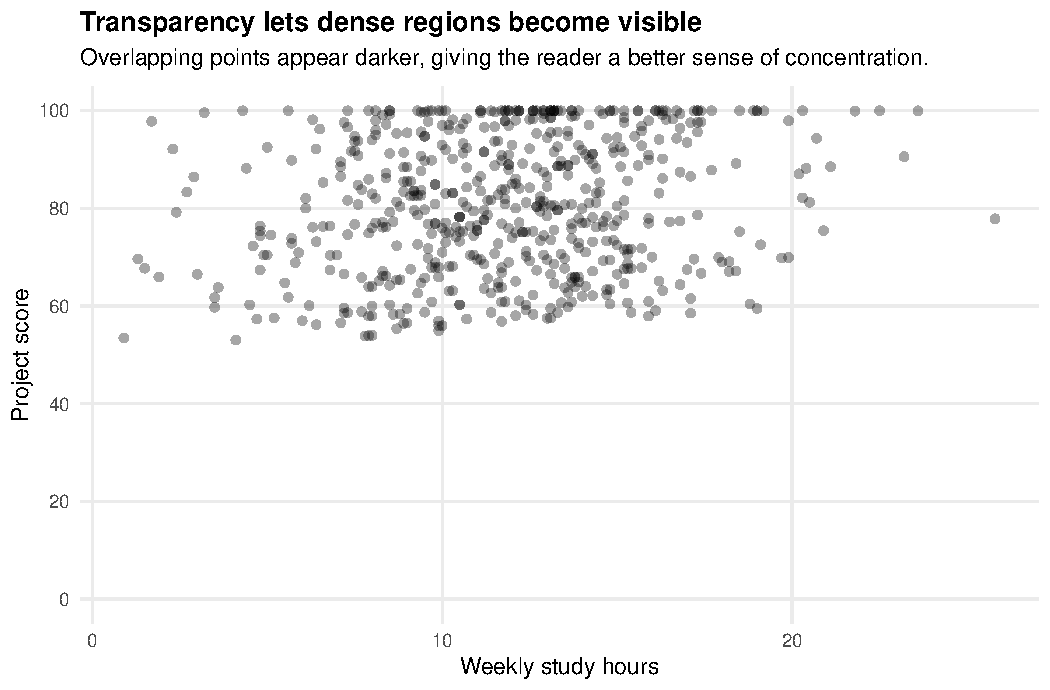
\includegraphics[width=0.9\linewidth,height=\textheight,keepaspectratio,alt={A scatter plot using transparency to make dense overlapping points easier to inspect.}]{chapters/17-clarity-and-control_files/figure-pdf/fig-17-overplotting-alpha-1.pdf}

}

\caption{\label{fig-17-overplotting-alpha}Alpha Blending Helps Reveal
Density in an Overplotted Scatter Plot}

\end{figure}%

The code in Listing~\ref{lst-fig-17-overplotting-alpha} produces
Figure~\ref{fig-17-overplotting-alpha}.

Figure 17.9 keeps individual points visible while reducing the false
impression that every point is equally isolated. When the dataset grows
much larger, Leo should consider binning.

\begin{codelisting}

\caption{\label{lst-fig-17-overplotting-bin2d}Code for 17 overplotting
bin2d}

\centering{

\begin{Shaded}
\begin{Highlighting}[]
\FunctionTok{ggplot}\NormalTok{(df\_analysis, }\FunctionTok{aes}\NormalTok{(}\AttributeTok{x =}\NormalTok{ study\_hours, }\AttributeTok{y =}\NormalTok{ project\_score)) }\SpecialCharTok{+}
  \FunctionTok{geom\_bin2d}\NormalTok{(}\AttributeTok{bins =} \DecValTok{25}\NormalTok{) }\SpecialCharTok{+}
  \FunctionTok{scale\_fill\_viridis\_c}\NormalTok{(}\AttributeTok{option =} \StringTok{"C"}\NormalTok{, }\AttributeTok{end =} \FloatTok{0.9}\NormalTok{) }\SpecialCharTok{+}
  \FunctionTok{scale\_y\_continuous}\NormalTok{(}\AttributeTok{limits =} \FunctionTok{c}\NormalTok{(}\DecValTok{0}\NormalTok{, }\DecValTok{100}\NormalTok{), }\AttributeTok{breaks =} \FunctionTok{seq}\NormalTok{(}\DecValTok{0}\NormalTok{, }\DecValTok{100}\NormalTok{, }\DecValTok{20}\NormalTok{)) }\SpecialCharTok{+}
  \FunctionTok{labs}\NormalTok{(}
    \AttributeTok{title =} \StringTok{"Binning is useful when density matters more than individual points"}\NormalTok{,}
    \AttributeTok{subtitle =} \StringTok{"Each rectangle counts how many observations fall into that region of the plot."}\NormalTok{,}
    \AttributeTok{x =} \StringTok{"Weekly study hours"}\NormalTok{,}
    \AttributeTok{y =} \StringTok{"Project score"}\NormalTok{,}
    \AttributeTok{fill =} \StringTok{"Learners"}
\NormalTok{  ) }\SpecialCharTok{+}
\NormalTok{  chapter17\_theme }\SpecialCharTok{+}
  \FunctionTok{theme}\NormalTok{(}\AttributeTok{legend.position =} \StringTok{"right"}\NormalTok{)}
\end{Highlighting}
\end{Shaded}

}

\end{codelisting}%

\begin{figure}[H]

\centering{

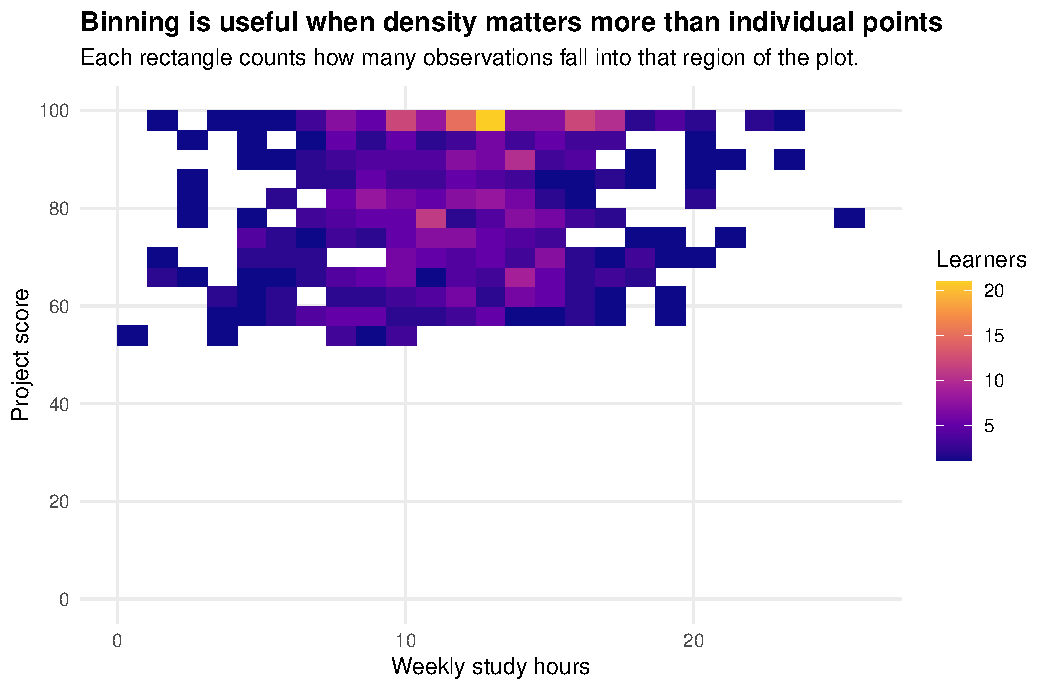
\includegraphics[width=0.9\linewidth,height=\textheight,keepaspectratio,alt={A binned two-dimensional plot showing point density where many observations overlap.}]{chapters/17-clarity-and-control_files/figure-pdf/fig-17-overplotting-bin2d-1.pdf}

}

\caption{\label{fig-17-overplotting-bin2d}Binning Converts Heavy
Overplotting into a Density Pattern}

\end{figure}%

The code in Listing~\ref{lst-fig-17-overplotting-bin2d} produces
Figure~\ref{fig-17-overplotting-bin2d}.

Figure 17.10 changes the question slightly. It no longer asks the reader
to inspect each point. It asks where observations are concentrated. That
is often the right question when the dataset is large.

\section{Label Collisions and Dense
Annotations}\label{label-collisions-and-dense-annotations}

Labels are useful only when they can be read. When labels overlap, the
plot becomes a puzzle.

The basic tools are:

\begin{itemize}
\tightlist
\item
  \texttt{geom\_text()} for text labels;
\item
  \texttt{geom\_label()} for text labels inside boxes;
\item
  \texttt{ggrepel::geom\_text\_repel()} and
  \texttt{ggrepel::geom\_label\_repel()} for automatic collision
  avoidance.
\end{itemize}

For crowded plots, Leo should treat \texttt{ggrepel} as the default
choice when label collisions are likely.

A simple example uses country-level summaries. The goal is to label the
groups without making the labels fight each other.

\begin{codelisting}

\caption{\label{lst-fig-17-label-collision-problem}Code for 17 label
collision problem}

\centering{

\begin{Shaded}
\begin{Highlighting}[]
\NormalTok{country\_summary }\OtherTok{\textless{}{-}}\NormalTok{ df\_analysis }\SpecialCharTok{|\textgreater{}}
  \FunctionTok{filter}\NormalTok{(}\SpecialCharTok{!}\FunctionTok{is.na}\NormalTok{(country), }\SpecialCharTok{!}\FunctionTok{is.na}\NormalTok{(study\_hours), }\SpecialCharTok{!}\FunctionTok{is.na}\NormalTok{(project\_score)) }\SpecialCharTok{|\textgreater{}}
  \FunctionTok{group\_by}\NormalTok{(country) }\SpecialCharTok{|\textgreater{}}
  \FunctionTok{summarise}\NormalTok{(}
    \AttributeTok{mean\_study\_hours =} \FunctionTok{mean}\NormalTok{(study\_hours, }\AttributeTok{na.rm =} \ConstantTok{TRUE}\NormalTok{),}
    \AttributeTok{mean\_project\_score =} \FunctionTok{mean}\NormalTok{(project\_score, }\AttributeTok{na.rm =} \ConstantTok{TRUE}\NormalTok{),}
    \AttributeTok{learners =} \FunctionTok{n}\NormalTok{(),}
    \AttributeTok{.groups =} \StringTok{"drop"}
\NormalTok{  )}

\FunctionTok{ggplot}\NormalTok{(country\_summary, }\FunctionTok{aes}\NormalTok{(}\AttributeTok{x =}\NormalTok{ mean\_study\_hours, }\AttributeTok{y =}\NormalTok{ mean\_project\_score, }\AttributeTok{label =}\NormalTok{ country)) }\SpecialCharTok{+}
  \FunctionTok{geom\_point}\NormalTok{(}\FunctionTok{aes}\NormalTok{(}\AttributeTok{size =}\NormalTok{ learners), }\AttributeTok{alpha =} \FloatTok{0.7}\NormalTok{) }\SpecialCharTok{+}
  \FunctionTok{geom\_text}\NormalTok{(}\AttributeTok{nudge\_y =} \DecValTok{2}\NormalTok{) }\SpecialCharTok{+}
  \FunctionTok{scale\_y\_continuous}\NormalTok{(}\AttributeTok{limits =} \FunctionTok{c}\NormalTok{(}\DecValTok{0}\NormalTok{, }\DecValTok{100}\NormalTok{), }\AttributeTok{breaks =} \FunctionTok{seq}\NormalTok{(}\DecValTok{0}\NormalTok{, }\DecValTok{100}\NormalTok{, }\DecValTok{20}\NormalTok{)) }\SpecialCharTok{+}
  \FunctionTok{labs}\NormalTok{(}
    \AttributeTok{title =} \StringTok{"Ordinary text labels can collide"}\NormalTok{,}
    \AttributeTok{subtitle =} \StringTok{"When labels compete for the same space, the reader loses the comparison."}\NormalTok{,}
    \AttributeTok{x =} \StringTok{"Average weekly study hours"}\NormalTok{,}
    \AttributeTok{y =} \StringTok{"Average project score"}\NormalTok{,}
    \AttributeTok{size =} \StringTok{"Learners"}
\NormalTok{  ) }\SpecialCharTok{+}
\NormalTok{  chapter17\_theme}
\end{Highlighting}
\end{Shaded}

}

\end{codelisting}%

\begin{figure}[H]

\centering{

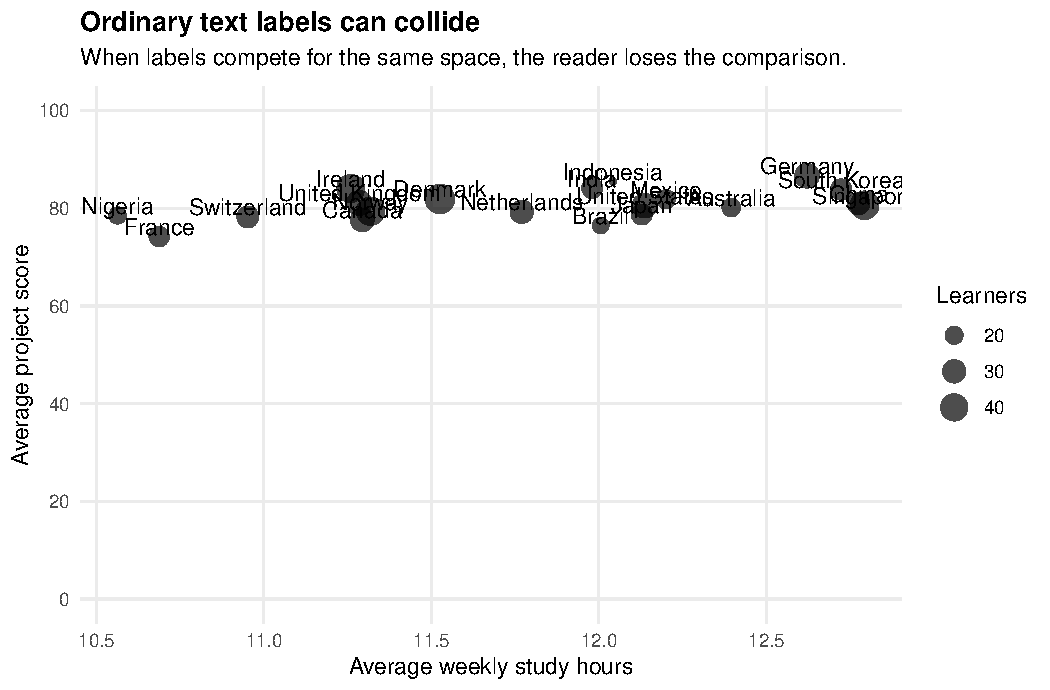
\includegraphics[width=0.9\linewidth,height=\textheight,keepaspectratio,alt={A plot with overlapping text labels that makes key information difficult to read.}]{chapters/17-clarity-and-control_files/figure-pdf/fig-17-label-collision-problem-1.pdf}

}

\caption{\label{fig-17-label-collision-problem}Label Collision Makes a
Plot Harder to Read}

\end{figure}%

The code in Listing~\ref{lst-fig-17-label-collision-problem} produces
Figure~\ref{fig-17-label-collision-problem}.

Figure~\ref{fig-17-label-collision-problem} shows the problem. The code
is simple, but simple is not always readable.

The better version uses \texttt{ggrepel}. Because \texttt{ggrepel} is an
additional package. It should run after the package is installed and
loaded.

\begin{codelisting}

\caption{\label{lst-fig-17-label-collision-ggrepel}Code for 17 label
collision ggrepel}

\centering{

\begin{Shaded}
\begin{Highlighting}[]
\FunctionTok{library}\NormalTok{(ggrepel)}

\FunctionTok{ggplot}\NormalTok{(country\_summary, }\FunctionTok{aes}\NormalTok{(}\AttributeTok{x =}\NormalTok{ mean\_study\_hours, }\AttributeTok{y =}\NormalTok{ mean\_project\_score, }\AttributeTok{label =}\NormalTok{ country)) }\SpecialCharTok{+}
  \FunctionTok{geom\_point}\NormalTok{(}\FunctionTok{aes}\NormalTok{(}\AttributeTok{size =}\NormalTok{ learners), }\AttributeTok{alpha =} \FloatTok{0.7}\NormalTok{) }\SpecialCharTok{+}
\NormalTok{  ggrepel}\SpecialCharTok{::}\FunctionTok{geom\_text\_repel}\NormalTok{(}\AttributeTok{max.overlaps =} \ConstantTok{Inf}\NormalTok{, }\AttributeTok{seed =} \DecValTok{1703}\NormalTok{) }\SpecialCharTok{+}
  \FunctionTok{scale\_y\_continuous}\NormalTok{(}\AttributeTok{limits =} \FunctionTok{c}\NormalTok{(}\DecValTok{0}\NormalTok{, }\DecValTok{100}\NormalTok{), }\AttributeTok{breaks =} \FunctionTok{seq}\NormalTok{(}\DecValTok{0}\NormalTok{, }\DecValTok{100}\NormalTok{, }\DecValTok{20}\NormalTok{)) }\SpecialCharTok{+}
  \FunctionTok{labs}\NormalTok{(}
    \AttributeTok{title =} \StringTok{"ggrepel moves labels away from collisions"}\NormalTok{,}
    \AttributeTok{subtitle =} \StringTok{"Labels remain attached to data points while avoiding unnecessary overlap."}\NormalTok{,}
    \AttributeTok{x =} \StringTok{"Average weekly study hours"}\NormalTok{,}
    \AttributeTok{y =} \StringTok{"Average project score"}\NormalTok{,}
    \AttributeTok{size =} \StringTok{"Learners"}
\NormalTok{  ) }\SpecialCharTok{+}
\NormalTok{  chapter17\_theme}
\end{Highlighting}
\end{Shaded}

}

\end{codelisting}%

\begin{figure}[H]

\centering{

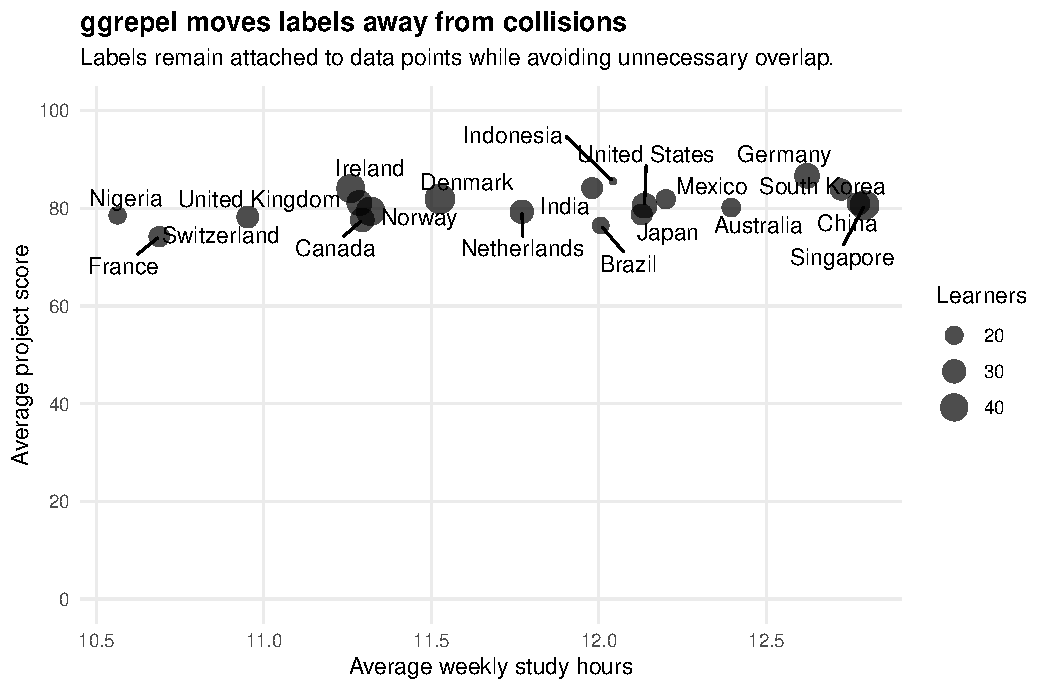
\includegraphics[width=0.9\linewidth,height=\textheight,keepaspectratio,alt={A plot using ggrepel to place labels with less overlap and better readability.}]{chapters/17-clarity-and-control_files/figure-pdf/fig-17-label-collision-ggrepel-1.pdf}

}

\caption{\label{fig-17-label-collision-ggrepel}Automatic Label Collision
Avoidance Using ggrepel}

\end{figure}%

The code in Listing~\ref{lst-fig-17-label-collision-ggrepel} produces
Figure~\ref{fig-17-label-collision-ggrepel} and shows the optional
\texttt{ggrepel} version Leo can use when labels are likely to collide.

This optional listing is the version Leo should prefer when labels are
likely to collide. \texttt{ggrepel} does not remove the need for
judgment. Too many labels can still overload a plot. But when a plot
genuinely needs labels, automatic repulsion is cleaner than hand-tuning
every label position.

\begin{tcolorbox}[enhanced jigsaw, arc=.35mm, bottomrule=.15mm, breakable, colback=white, colframe=quarto-callout-warning-color-frame, left=2mm, leftrule=.75mm, opacityback=0, rightrule=.15mm, toprule=.15mm]
\begin{minipage}[t]{5.5mm}
\textcolor{quarto-callout-warning-color}{\faExclamationTriangle}
\end{minipage}%
\begin{minipage}[t]{\textwidth - 5.5mm}

\vspace{-3mm}\textbf{Do not label everything}\vspace{3mm}

A label is a request for attention. If every point is labelled, no point
is emphasized. Label the values that help the reader understand the main
comparison.

\end{minipage}%
\end{tcolorbox}

\section{Mathematical Annotation and Rich
Text}\label{mathematical-annotation-and-rich-text}

Some plots need more than ordinary labels. A model line may need an
equation. A scientific chart may need notation. A report figure may need
a title with emphasis inside the text.

Useful tools include:

\begin{itemize}
\tightlist
\item
  \texttt{annotate()} for adding text or shapes at specific plot
  locations;
\item
  \texttt{expression()} and plotmath syntax for mathematical notation;
\item
  \texttt{ggtext::element\_markdown()} when titles, subtitles, or axis
  labels need markdown or simple HTML styling.
\end{itemize}

For ordinary annotation, \texttt{annotate()} is often enough.

\begin{codelisting}

\caption{\label{lst-fig-17-annotation}Code for 17 annotation}

\centering{

\begin{Shaded}
\begin{Highlighting}[]
\FunctionTok{ggplot}\NormalTok{(df\_analysis, }\FunctionTok{aes}\NormalTok{(}\AttributeTok{x =}\NormalTok{ study\_hours, }\AttributeTok{y =}\NormalTok{ project\_score)) }\SpecialCharTok{+}
  \FunctionTok{geom\_point}\NormalTok{(}\AttributeTok{alpha =} \FloatTok{0.30}\NormalTok{) }\SpecialCharTok{+}
  \FunctionTok{geom\_smooth}\NormalTok{(}\AttributeTok{method =} \StringTok{"lm"}\NormalTok{, }\AttributeTok{se =} \ConstantTok{FALSE}\NormalTok{, }\AttributeTok{linewidth =} \FloatTok{0.8}\NormalTok{) }\SpecialCharTok{+}
  \FunctionTok{annotate}\NormalTok{(}
    \StringTok{"label"}\NormalTok{,}
    \AttributeTok{x =} \DecValTok{2}\NormalTok{,}
    \AttributeTok{y =} \DecValTok{95}\NormalTok{,}
    \AttributeTok{hjust =} \DecValTok{0}\NormalTok{,}
    \AttributeTok{label =} \StringTok{"The fitted line summarizes the general direction,}\SpecialCharTok{\textbackslash{}n}\StringTok{not the performance of every learner."}\NormalTok{,}
    \AttributeTok{size =} \FloatTok{3.2}\NormalTok{,}
    \AttributeTok{label.size =} \FloatTok{0.2}
\NormalTok{  ) }\SpecialCharTok{+}
  \FunctionTok{scale\_y\_continuous}\NormalTok{(}\AttributeTok{limits =} \FunctionTok{c}\NormalTok{(}\DecValTok{0}\NormalTok{, }\DecValTok{100}\NormalTok{), }\AttributeTok{breaks =} \FunctionTok{seq}\NormalTok{(}\DecValTok{0}\NormalTok{, }\DecValTok{100}\NormalTok{, }\DecValTok{20}\NormalTok{)) }\SpecialCharTok{+}
  \FunctionTok{labs}\NormalTok{(}
    \AttributeTok{title =} \StringTok{"Annotation can guide interpretation inside the plot"}\NormalTok{,}
    \AttributeTok{x =} \StringTok{"Weekly study hours"}\NormalTok{,}
    \AttributeTok{y =} \StringTok{"Project score"}
\NormalTok{  ) }\SpecialCharTok{+}
\NormalTok{  chapter17\_theme}
\end{Highlighting}
\end{Shaded}

}

\end{codelisting}%

\begin{figure}[H]

\centering{

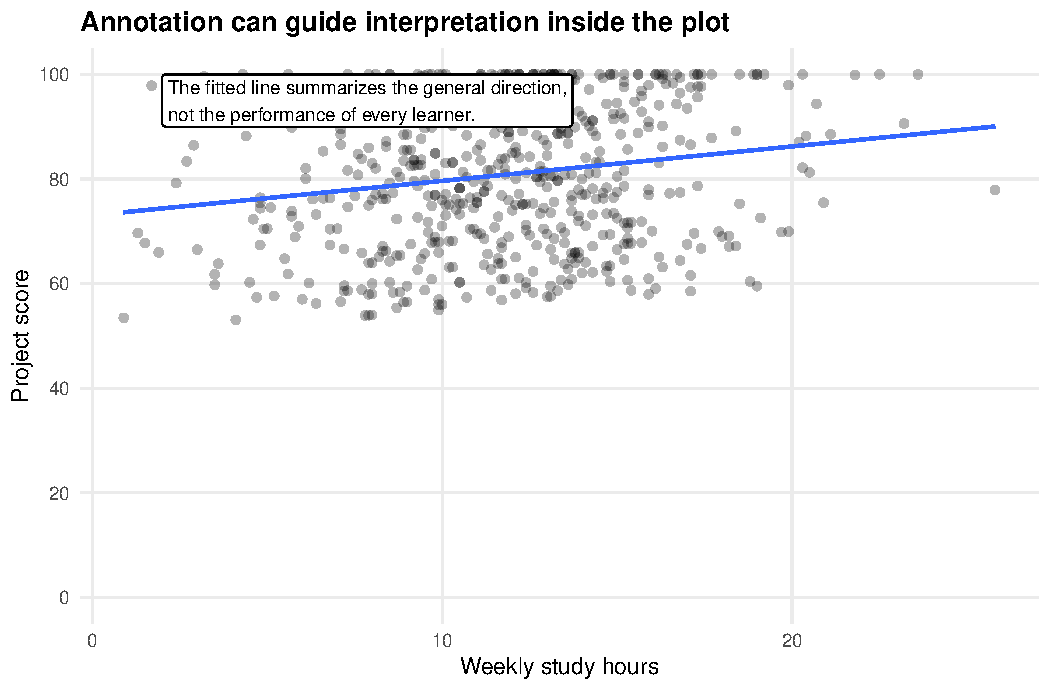
\includegraphics[width=0.9\linewidth,height=\textheight,keepaspectratio,alt={A plot with direct annotation explaining an important pattern without requiring the reader to rely only on the legend.}]{chapters/17-clarity-and-control_files/figure-pdf/fig-17-annotation-1.pdf}

}

\caption{\label{fig-17-annotation}Direct Annotation Can Explain the
Pattern Without Overloading the Legend}

\end{figure}%

The code in Listing~\ref{lst-fig-17-annotation} produces
Figure~\ref{fig-17-annotation}.

Figure 17.13 uses annotation to prevent overinterpretation. The note
explains what the smooth line does and does not mean.

For mathematical notation, plotmath can be useful.

\begin{codelisting}

\caption{\label{lst-fig-17-math-annotation}Code for 17 math annotation}

\centering{

\begin{Shaded}
\begin{Highlighting}[]
\FunctionTok{ggplot}\NormalTok{(df\_analysis, }\FunctionTok{aes}\NormalTok{(}\AttributeTok{x =}\NormalTok{ study\_hours, }\AttributeTok{y =}\NormalTok{ project\_score)) }\SpecialCharTok{+}
  \FunctionTok{geom\_point}\NormalTok{(}\AttributeTok{alpha =} \FloatTok{0.30}\NormalTok{) }\SpecialCharTok{+}
  \FunctionTok{geom\_smooth}\NormalTok{(}\AttributeTok{method =} \StringTok{"lm"}\NormalTok{, }\AttributeTok{se =} \ConstantTok{FALSE}\NormalTok{, }\AttributeTok{linewidth =} \FloatTok{0.8}\NormalTok{) }\SpecialCharTok{+}
  \FunctionTok{annotate}\NormalTok{(}
    \StringTok{"text"}\NormalTok{,}
    \AttributeTok{x =} \DecValTok{2}\NormalTok{,}
    \AttributeTok{y =} \DecValTok{90}\NormalTok{,}
    \AttributeTok{hjust =} \DecValTok{0}\NormalTok{,}
    \AttributeTok{label =} \StringTok{"italic(y) == beta[0] + beta[1] * italic(x) + epsilon"}\NormalTok{,}
    \AttributeTok{parse =} \ConstantTok{TRUE}\NormalTok{,}
    \AttributeTok{size =} \DecValTok{4}
\NormalTok{  ) }\SpecialCharTok{+}
  \FunctionTok{scale\_y\_continuous}\NormalTok{(}\AttributeTok{limits =} \FunctionTok{c}\NormalTok{(}\DecValTok{0}\NormalTok{, }\DecValTok{100}\NormalTok{), }\AttributeTok{breaks =} \FunctionTok{seq}\NormalTok{(}\DecValTok{0}\NormalTok{, }\DecValTok{100}\NormalTok{, }\DecValTok{20}\NormalTok{)) }\SpecialCharTok{+}
  \FunctionTok{labs}\NormalTok{(}
    \AttributeTok{title =} \StringTok{"Mathematical annotation is useful when notation clarifies the model"}\NormalTok{,}
    \AttributeTok{x =} \StringTok{"Weekly study hours"}\NormalTok{,}
    \AttributeTok{y =} \StringTok{"Project score"}
\NormalTok{  ) }\SpecialCharTok{+}
\NormalTok{  chapter17\_theme}
\end{Highlighting}
\end{Shaded}

}

\end{codelisting}%

\begin{figure}[H]

\centering{

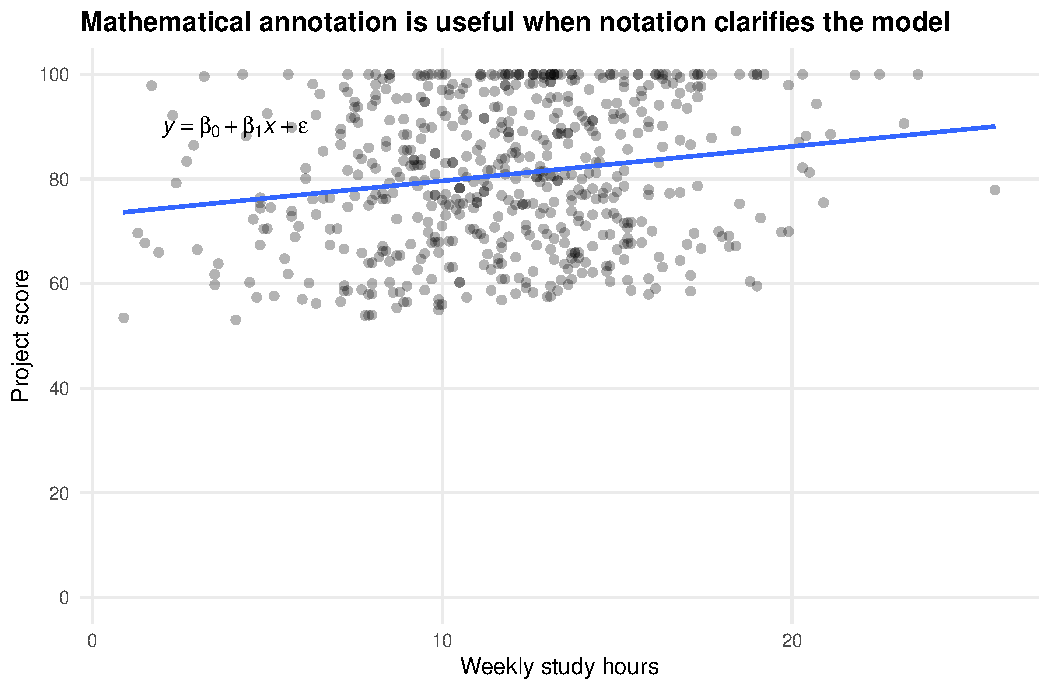
\includegraphics[width=0.9\linewidth,height=\textheight,keepaspectratio,alt={A plot showing enhanced scientific or mathematical annotation inside a ggplot2 figure.}]{chapters/17-clarity-and-control_files/figure-pdf/fig-17-math-annotation-1.pdf}

}

\caption{\label{fig-17-math-annotation}Enhanced Scientific Annotation in
ggplot2}

\end{figure}%

The code in Listing~\ref{lst-fig-17-math-annotation} produces
Figure~\ref{fig-17-math-annotation}.

Figure 17.14 shows a compact model notation. The point is not to make
the plot look advanced. The point is to help readers connect the visual
line with the idea of a model.

When Leo needs markdown styling in titles or labels, \texttt{ggtext} can
help. The following example is non-evaluated because it requires the
additional package.

\begin{codelisting}

\caption{\label{lst-code-ggtext-example}Code for Ggtext example}

\centering{

\begin{Shaded}
\begin{Highlighting}[]
\FunctionTok{library}\NormalTok{(ggtext)}

\FunctionTok{ggplot}\NormalTok{(df\_analysis, }\FunctionTok{aes}\NormalTok{(}\AttributeTok{x =}\NormalTok{ study\_hours, }\AttributeTok{y =}\NormalTok{ project\_score)) }\SpecialCharTok{+}
  \FunctionTok{geom\_point}\NormalTok{(}\AttributeTok{alpha =} \FloatTok{0.30}\NormalTok{) }\SpecialCharTok{+}
  \FunctionTok{labs}\NormalTok{(}
    \AttributeTok{title =} \StringTok{"Project score rises with \textless{}b\textgreater{}study time\textless{}/b\textgreater{}, but variation remains"}\NormalTok{,}
    \AttributeTok{x =} \StringTok{"Weekly study hours"}\NormalTok{,}
    \AttributeTok{y =} \StringTok{"Project score"}
\NormalTok{  ) }\SpecialCharTok{+}
  \FunctionTok{theme\_minimal}\NormalTok{() }\SpecialCharTok{+}
  \FunctionTok{theme}\NormalTok{(}\AttributeTok{plot.title =}\NormalTok{ ggtext}\SpecialCharTok{::}\FunctionTok{element\_markdown}\NormalTok{())}
\end{Highlighting}
\end{Shaded}

}

\end{codelisting}%

The code in Listing~\ref{lst-code-ggtext-example} shows the code pattern
being discussed here.

\texttt{ggtext} is helpful when ordinary text controls are too rigid. It
should not be used to turn titles into decorative banners. It is a tool
for controlled emphasis.

\section{Aspect Ratios and Plot
Geometry}\label{aspect-ratios-and-plot-geometry}

The same data can feel different when the plot is stretched, squeezed,
widened, or narrowed. This is especially important for line charts,
maps, spatial plots, and any chart where slope or shape affects
interpretation.

Aspect ratio is the relationship between the height and width of the
plotting panel. In \texttt{ggplot2}, Leo can control it with:

\begin{itemize}
\tightlist
\item
  \texttt{theme(aspect.ratio\ =\ ...)} for general panel proportions;
\item
  \texttt{coord\_fixed()} when one unit on the x-axis should have the
  same physical length as one unit on the y-axis.
\end{itemize}

\begin{codelisting}

\caption{\label{lst-fig-17-aspect-ratio}Code for 17 aspect ratio}

\centering{

\begin{Shaded}
\begin{Highlighting}[]
\NormalTok{weekly\_scores }\SpecialCharTok{|\textgreater{}}
  \FunctionTok{ggplot}\NormalTok{(}\FunctionTok{aes}\NormalTok{(}\AttributeTok{x =}\NormalTok{ week, }\AttributeTok{y =}\NormalTok{ mean\_project\_score)) }\SpecialCharTok{+}
  \FunctionTok{geom\_line}\NormalTok{(}\AttributeTok{linewidth =} \FloatTok{0.8}\NormalTok{) }\SpecialCharTok{+}
  \FunctionTok{geom\_point}\NormalTok{(}\AttributeTok{size =} \DecValTok{2}\NormalTok{) }\SpecialCharTok{+}
  \FunctionTok{scale\_x\_continuous}\NormalTok{(}\AttributeTok{breaks =} \FunctionTok{sort}\NormalTok{(}\FunctionTok{unique}\NormalTok{(weekly\_scores}\SpecialCharTok{$}\NormalTok{week))) }\SpecialCharTok{+}
  \FunctionTok{scale\_y\_continuous}\NormalTok{(}\AttributeTok{limits =} \FunctionTok{c}\NormalTok{(}\DecValTok{0}\NormalTok{, }\DecValTok{100}\NormalTok{), }\AttributeTok{breaks =} \FunctionTok{seq}\NormalTok{(}\DecValTok{0}\NormalTok{, }\DecValTok{100}\NormalTok{, }\DecValTok{20}\NormalTok{)) }\SpecialCharTok{+}
  \FunctionTok{labs}\NormalTok{(}
    \AttributeTok{title =} \StringTok{"Aspect ratio can change how steep a pattern feels"}\NormalTok{,}
    \AttributeTok{subtitle =} \StringTok{"The data are unchanged, but panel shape affects visual judgment."}\NormalTok{,}
    \AttributeTok{x =} \StringTok{"Learning week"}\NormalTok{,}
    \AttributeTok{y =} \StringTok{"Average project score"}
\NormalTok{  ) }\SpecialCharTok{+}
\NormalTok{  chapter17\_theme }\SpecialCharTok{+}
  \FunctionTok{theme}\NormalTok{(}\AttributeTok{aspect.ratio =} \FloatTok{0.55}\NormalTok{)}
\end{Highlighting}
\end{Shaded}

}

\end{codelisting}%

\begin{figure}[H]

\centering{

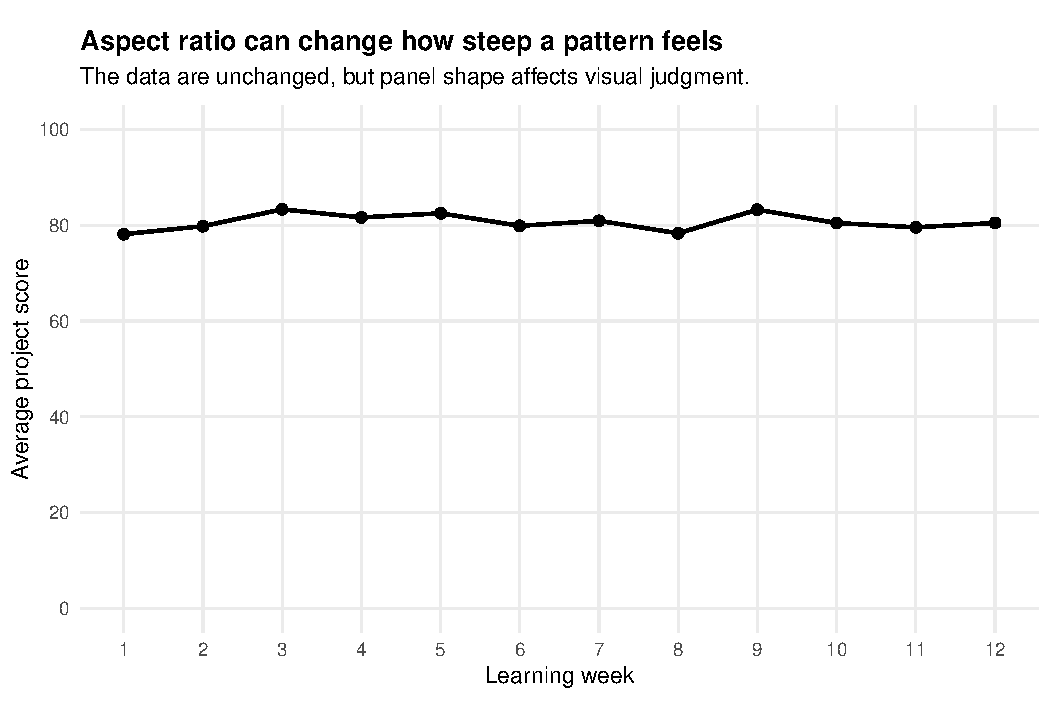
\includegraphics[width=0.9\linewidth,height=\textheight,keepaspectratio,alt={Two visual presentations showing how aspect ratio can change how steep or flat a pattern appears.}]{chapters/17-clarity-and-control_files/figure-pdf/fig-17-aspect-ratio-1.pdf}

}

\caption{\label{fig-17-aspect-ratio}How Aspect Ratio Changes
Interpretation}

\end{figure}%

The code in Listing~\ref{lst-fig-17-aspect-ratio} produces
Figure~\ref{fig-17-aspect-ratio}.

Figure 17.15 uses \texttt{theme(aspect.ratio\ =\ 0.55)} to set the panel
relationship deliberately. The key lesson is not the exact number. The
lesson is that plot dimensions are part of interpretation.

\begin{tcolorbox}[enhanced jigsaw, arc=.35mm, bottomrule=.15mm, breakable, colback=white, colframe=quarto-callout-note-color-frame, left=2mm, leftrule=.75mm, opacityback=0, rightrule=.15mm, toprule=.15mm]
\begin{minipage}[t]{5.5mm}
\textcolor{quarto-callout-note-color}{\faInfo}
\end{minipage}%
\begin{minipage}[t]{\textwidth - 5.5mm}

\vspace{-3mm}\textbf{When aspect ratio matters most}\vspace{3mm}

Aspect ratio deserves special attention when readers may judge slope,
distance, shape, or spatial relationship. For ordinary bar charts, it
may matter less. For line charts, maps, and coordinate comparisons, it
can matter a great deal.

\end{minipage}%
\end{tcolorbox}

\section{Zooming Without Lying}\label{zooming-without-lying}

Sometimes Leo needs to look closely at a region of a plot. That is
reasonable. But there are different ways to narrow attention, and they
do not behave the same way.

He must distinguish among:

\begin{itemize}
\tightlist
\item
  \textbf{filtering data}, which removes observations before plotting;
\item
  \textbf{scale limits}, which may remove observations before some
  calculations are drawn;
\item
  \textbf{coordinate zooming}, which changes the visible window without
  dropping data from the underlying plot calculation.
\end{itemize}

When the goal is to zoom without clipping the data used by layers,
\texttt{coord\_cartesian()} is often safer.

\begin{codelisting}

\caption{\label{lst-fig-17-coord-cartesian}Code for 17 coord cartesian}

\centering{

\begin{Shaded}
\begin{Highlighting}[]
\FunctionTok{ggplot}\NormalTok{(df\_analysis, }\FunctionTok{aes}\NormalTok{(}\AttributeTok{x =}\NormalTok{ study\_hours, }\AttributeTok{y =}\NormalTok{ project\_score)) }\SpecialCharTok{+}
  \FunctionTok{geom\_point}\NormalTok{(}\AttributeTok{alpha =} \FloatTok{0.30}\NormalTok{) }\SpecialCharTok{+}
  \FunctionTok{geom\_smooth}\NormalTok{(}\AttributeTok{method =} \StringTok{"lm"}\NormalTok{, }\AttributeTok{se =} \ConstantTok{FALSE}\NormalTok{, }\AttributeTok{linewidth =} \FloatTok{0.8}\NormalTok{) }\SpecialCharTok{+}
  \FunctionTok{coord\_cartesian}\NormalTok{(}\AttributeTok{ylim =} \FunctionTok{c}\NormalTok{(}\DecValTok{40}\NormalTok{, }\DecValTok{100}\NormalTok{)) }\SpecialCharTok{+}
  \FunctionTok{labs}\NormalTok{(}
    \AttributeTok{title =} \StringTok{"coord\_cartesian() changes the viewing window"}\NormalTok{,}
    \AttributeTok{subtitle =} \StringTok{"The plot zooms into the upper score range without filtering rows first."}\NormalTok{,}
    \AttributeTok{x =} \StringTok{"Weekly study hours"}\NormalTok{,}
    \AttributeTok{y =} \StringTok{"Project score"}
\NormalTok{  ) }\SpecialCharTok{+}
\NormalTok{  chapter17\_theme}
\end{Highlighting}
\end{Shaded}

}

\end{codelisting}%

\begin{figure}[H]

\centering{

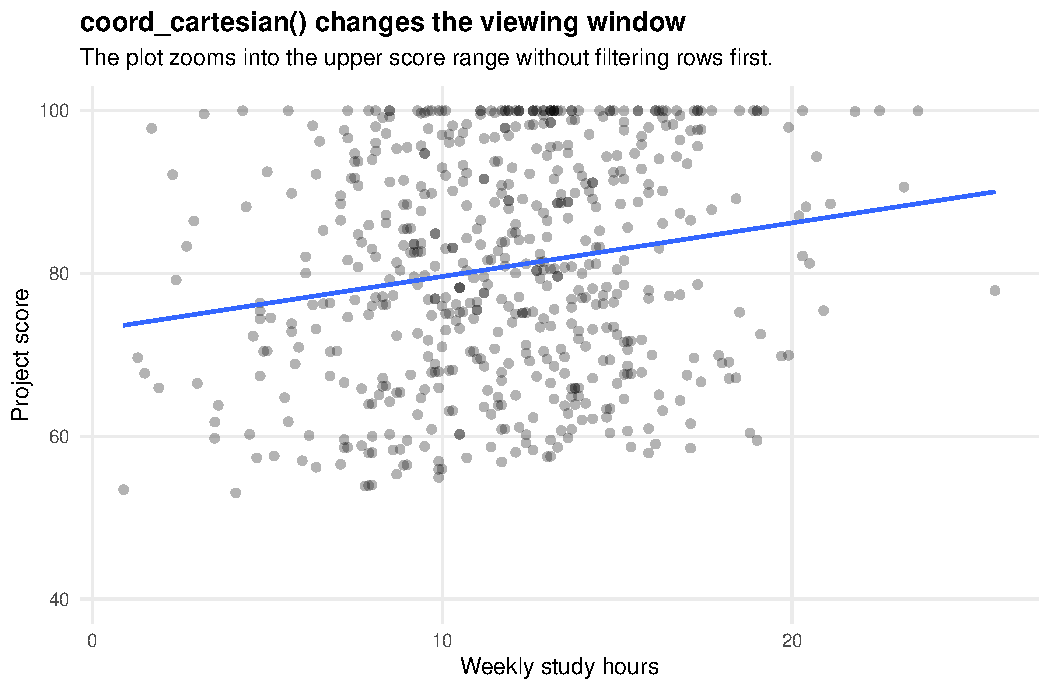
\includegraphics[width=0.9\linewidth,height=\textheight,keepaspectratio,alt={A zoomed plot view created with coord\_cartesian, preserving the data used in the plot calculation.}]{chapters/17-clarity-and-control_files/figure-pdf/fig-17-coord-cartesian-1.pdf}

}

\caption{\label{fig-17-coord-cartesian}coord\_cartesian() Zooms the View
Without Removing Data from the Plot Calculation}

\end{figure}%

The code in Listing~\ref{lst-fig-17-coord-cartesian} produces
Figure~\ref{fig-17-coord-cartesian}.

Figure 17.16 does not claim that low scores do not exist. It zooms the
view so a particular region can be examined. The caption and subtitle
make that clear.

\begin{tcolorbox}[enhanced jigsaw, arc=.35mm, bottomrule=.15mm, breakable, colback=white, colframe=quarto-callout-warning-color-frame, left=2mm, leftrule=.75mm, opacityback=0, rightrule=.15mm, toprule=.15mm]
\begin{minipage}[t]{5.5mm}
\textcolor{quarto-callout-warning-color}{\faExclamationTriangle}
\end{minipage}%
\begin{minipage}[t]{\textwidth - 5.5mm}

\vspace{-3mm}\textbf{Zoom honestly}\vspace{3mm}

If Leo zooms into a plot, he should make that choice visible in the
title, subtitle, caption, or axis labels. A zoomed chart should not
pretend to show the full range when it does not.

\end{minipage}%
\end{tcolorbox}

\section{Building Multi-Panel
Visualisations}\label{building-multi-panel-visualisations}

Faceting is the first multi-panel tool Leo met in Chapter 16. It remains
useful when the same plot should be repeated across groups. But
sometimes he needs more control than facets provide.

For publication layouts, he may need to combine different plot types,
align axes, control relative widths, or arrange panels in a precise
order. Two useful packages are:

\begin{itemize}
\tightlist
\item
  \texttt{patchwork}, which combines ggplot objects with a simple layout
  syntax;
\item
  \texttt{cowplot}, which provides careful alignment and plot assembly
  tools.
\end{itemize}

Use faceting when the panels share the same structure. Use
\texttt{patchwork} or \texttt{cowplot} when the panels are different
plots that need to appear together.

\begin{codelisting}

\caption{\label{lst-fig-17-patchwork-layout}Code for 17 patchwork
layout}

\centering{

\begin{Shaded}
\begin{Highlighting}[]
\FunctionTok{library}\NormalTok{(patchwork)}

\NormalTok{p1 }\OtherTok{\textless{}{-}} \FunctionTok{ggplot}\NormalTok{(df\_analysis, }\FunctionTok{aes}\NormalTok{(}\AttributeTok{x =}\NormalTok{ study\_hours, }\AttributeTok{y =}\NormalTok{ project\_score)) }\SpecialCharTok{+}
  \FunctionTok{geom\_point}\NormalTok{(}\AttributeTok{alpha =} \FloatTok{0.30}\NormalTok{) }\SpecialCharTok{+}
  \FunctionTok{geom\_smooth}\NormalTok{(}\AttributeTok{method =} \StringTok{"lm"}\NormalTok{, }\AttributeTok{se =} \ConstantTok{FALSE}\NormalTok{) }\SpecialCharTok{+}
  \FunctionTok{labs}\NormalTok{(}
    \AttributeTok{title =} \StringTok{"Study time and project score"}\NormalTok{,}
    \AttributeTok{x =} \StringTok{"Weekly study hours"}\NormalTok{,}
    \AttributeTok{y =} \StringTok{"Project score"}
\NormalTok{  ) }\SpecialCharTok{+}
\NormalTok{  chapter17\_theme}

\NormalTok{p2 }\OtherTok{\textless{}{-}}\NormalTok{ df\_analysis }\SpecialCharTok{|\textgreater{}}
  \FunctionTok{filter}\NormalTok{(}\SpecialCharTok{!}\FunctionTok{is.na}\NormalTok{(study\_band), }\SpecialCharTok{!}\FunctionTok{is.na}\NormalTok{(project\_score)) }\SpecialCharTok{|\textgreater{}}
  \FunctionTok{group\_by}\NormalTok{(study\_band) }\SpecialCharTok{|\textgreater{}}
  \FunctionTok{summarise}\NormalTok{(}\AttributeTok{mean\_project\_score =} \FunctionTok{mean}\NormalTok{(project\_score, }\AttributeTok{na.rm =} \ConstantTok{TRUE}\NormalTok{), }\AttributeTok{.groups =} \StringTok{"drop"}\NormalTok{) }\SpecialCharTok{|\textgreater{}}
  \FunctionTok{ggplot}\NormalTok{(}\FunctionTok{aes}\NormalTok{(}\AttributeTok{x =}\NormalTok{ study\_band, }\AttributeTok{y =}\NormalTok{ mean\_project\_score)) }\SpecialCharTok{+}
  \FunctionTok{geom\_col}\NormalTok{() }\SpecialCharTok{+}
  \FunctionTok{coord\_flip}\NormalTok{() }\SpecialCharTok{+}
  \FunctionTok{labs}\NormalTok{(}
    \AttributeTok{title =} \StringTok{"Average score by study band"}\NormalTok{,}
    \AttributeTok{x =} \ConstantTok{NULL}\NormalTok{,}
    \AttributeTok{y =} \StringTok{"Average project score"}
\NormalTok{  ) }\SpecialCharTok{+}
\NormalTok{  chapter17\_theme}

\NormalTok{p1 }\SpecialCharTok{+}\NormalTok{ p2 }\SpecialCharTok{+} \FunctionTok{plot\_layout}\NormalTok{(}\AttributeTok{widths =} \FunctionTok{c}\NormalTok{(}\DecValTok{2}\NormalTok{, }\DecValTok{1}\NormalTok{))}
\end{Highlighting}
\end{Shaded}

}

\end{codelisting}%

\begin{figure}[H]

\centering{

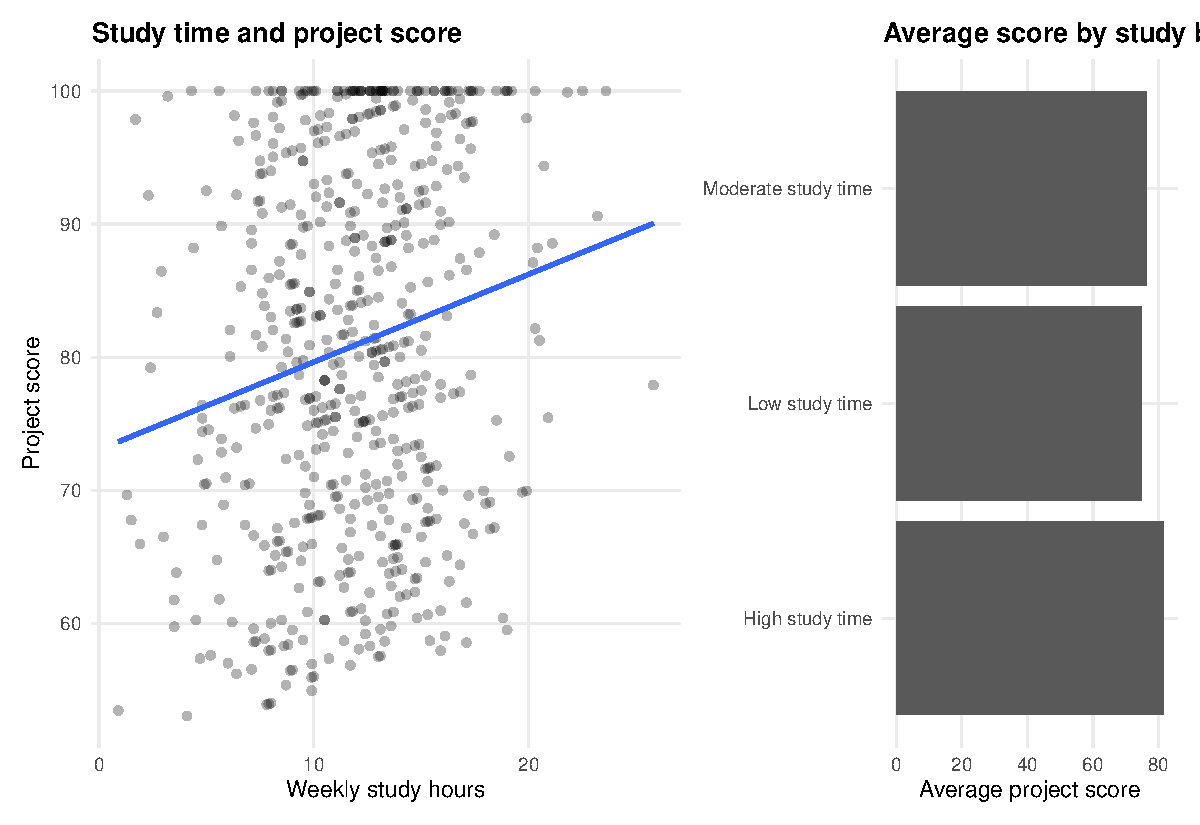
\includegraphics[width=0.9\linewidth,height=\textheight,keepaspectratio,alt={A multi-panel layout created with patchwork to organise related plots into one visual arrangement.}]{chapters/17-clarity-and-control_files/figure-pdf/fig-17-patchwork-layout-1.pdf}

}

\caption{\label{fig-17-patchwork-layout}Multi-Plot Layout Using
patchwork}

\end{figure}%

The code in Listing~\ref{lst-fig-17-patchwork-layout} produces
Figure~\ref{fig-17-patchwork-layout} and shows the \texttt{patchwork}
version Leo can use for multi-plot layout.

This optional listing shows the kind of layout problem
\texttt{patchwork} solves. Leo is not using it because faceting failed.
He is using it because the two panels answer related but different
visual questions.

For highly controlled alignment, \texttt{cowplot} is another option.

\begin{codelisting}

\caption{\label{lst-code-cowplot-layout}Code for Cowplot layout}

\centering{

\begin{Shaded}
\begin{Highlighting}[]
\FunctionTok{library}\NormalTok{(cowplot)}

\NormalTok{cowplot}\SpecialCharTok{::}\FunctionTok{plot\_grid}\NormalTok{(}
\NormalTok{  p1,}
\NormalTok{  p2,}
  \AttributeTok{labels =} \FunctionTok{c}\NormalTok{(}\StringTok{"A"}\NormalTok{, }\StringTok{"B"}\NormalTok{),}
  \AttributeTok{ncol =} \DecValTok{2}\NormalTok{,}
  \AttributeTok{rel\_widths =} \FunctionTok{c}\NormalTok{(}\DecValTok{2}\NormalTok{, }\DecValTok{1}\NormalTok{),}
  \AttributeTok{align =} \StringTok{"h"}
\NormalTok{)}
\end{Highlighting}
\end{Shaded}

}

\end{codelisting}%

The code in Listing~\ref{lst-code-cowplot-layout} shows the code pattern
being discussed here.

The professional decision is not which package is fashionable. The
decision is what layout problem Leo is solving.

\section{Introducing Interactivity}\label{introducing-interactivity}

Static graphics are still central to reports, articles, books, and
printed outputs. A static plot must stand on its own. It should not
require hovering, clicking, or zooming to make the central point
visible.

But some tasks are exploratory. Leo may want the reader to hover over a
point, inspect an individual learner, zoom into a dense region, or
compare details that would clutter a static chart.

That is where interactivity can help.

Two common tools are:

\begin{itemize}
\tightlist
\item
  \texttt{plotly}, often used through \texttt{ggplotly()} to convert a
  ggplot object into an interactive plot;
\item
  \texttt{ggiraph}, which provides interactive geoms with tooltips and
  hover effects.
\end{itemize}

\begin{codelisting}

\caption{\label{lst-tbl-17-4}Code for 17 4}

\centering{

\begin{Shaded}
\begin{Highlighting}[]
\NormalTok{interactive\_table }\OtherTok{\textless{}{-}}\NormalTok{ tibble}\SpecialCharTok{::}\FunctionTok{tribble}\NormalTok{(}
  \SpecialCharTok{\textasciitilde{}}\NormalTok{Need, }\SpecialCharTok{\textasciitilde{}}\NormalTok{Static\_graphic, }\SpecialCharTok{\textasciitilde{}}\NormalTok{Interactive\_graphic, }\SpecialCharTok{\textasciitilde{}}\NormalTok{Useful\_tool,}
  \StringTok{"Printed report or journal figure"}\NormalTok{, }\StringTok{"Usually best"}\NormalTok{, }\StringTok{"Usually not available"}\NormalTok{, }\StringTok{"ggplot2"}\NormalTok{,}
  \StringTok{"Reader must see the main pattern immediately"}\NormalTok{, }\StringTok{"Best choice"}\NormalTok{, }\StringTok{"Can support but should not replace clarity"}\NormalTok{, }\StringTok{"ggplot2"}\NormalTok{,}
  \StringTok{"Reader needs point{-}level details"}\NormalTok{, }\StringTok{"May become cluttered"}\NormalTok{, }\StringTok{"Hover text can help"}\NormalTok{, }\StringTok{"plotly or ggiraph"}\NormalTok{,}
  \StringTok{"Dense exploratory data"}\NormalTok{, }\StringTok{"May need binning or summaries"}\NormalTok{, }\StringTok{"Zooming and hover can support exploration"}\NormalTok{, }\StringTok{"plotly"}\NormalTok{,}
  \StringTok{"Teaching or dashboard{-}like exploration"}\NormalTok{, }\StringTok{"Useful for fixed explanation"}\NormalTok{, }\StringTok{"Useful for guided exploration"}\NormalTok{, }\StringTok{"ggiraph or plotly"}
\NormalTok{)}

\NormalTok{knitr}\SpecialCharTok{::}\FunctionTok{kable}\NormalTok{(interactive\_table)}
\end{Highlighting}
\end{Shaded}

}

\end{codelisting}%

{

\begin{longtable}[]{@{}
  >{\raggedright\arraybackslash}p{(\linewidth - 6\tabcolsep) * \real{0.3309}}
  >{\raggedright\arraybackslash}p{(\linewidth - 6\tabcolsep) * \real{0.2206}}
  >{\raggedright\arraybackslash}p{(\linewidth - 6\tabcolsep) * \real{0.3162}}
  >{\raggedright\arraybackslash}p{(\linewidth - 6\tabcolsep) * \real{0.1324}}@{}}

\caption{\label{tbl-17-4}Static versus Interactive Graphics}

\tabularnewline

\toprule\noalign{}
\begin{minipage}[b]{\linewidth}\raggedright
Need
\end{minipage} & \begin{minipage}[b]{\linewidth}\raggedright
Static\_graphic
\end{minipage} & \begin{minipage}[b]{\linewidth}\raggedright
Interactive\_graphic
\end{minipage} & \begin{minipage}[b]{\linewidth}\raggedright
Useful\_tool
\end{minipage} \\
\midrule\noalign{}
\endhead
\bottomrule\noalign{}
\endlastfoot
Printed report or journal figure & Usually best & Usually not available
& ggplot2 \\
Reader must see the main pattern immediately & Best choice & Can support
but should not replace clarity & ggplot2 \\
Reader needs point-level details & May become cluttered & Hover text can
help & plotly or ggiraph \\
Dense exploratory data & May need binning or summaries & Zooming and
hover can support exploration & plotly \\
Teaching or dashboard-like exploration & Useful for fixed explanation &
Useful for guided exploration & ggiraph or plotly \\

\end{longtable}

}

The code in Listing~\ref{lst-tbl-17-4} produces Table~\ref{tbl-17-4}.

Table 17.4 makes the boundary clear. Interactivity is not a rescue for
unclear thinking. It is useful when the task genuinely requires
exploration.

\begin{codelisting}

\caption{\label{lst-code-plotly-example}Code for Plotly example}

\centering{

\begin{Shaded}
\begin{Highlighting}[]
\FunctionTok{library}\NormalTok{(plotly)}

\NormalTok{p }\OtherTok{\textless{}{-}} \FunctionTok{ggplot}\NormalTok{(}
\NormalTok{  df\_analysis,}
  \FunctionTok{aes}\NormalTok{(}
    \AttributeTok{x =}\NormalTok{ study\_hours,}
    \AttributeTok{y =}\NormalTok{ project\_score,}
    \AttributeTok{text =} \FunctionTok{paste}\NormalTok{(}
      \StringTok{"Learner:"}\NormalTok{, learner\_id,}
      \StringTok{"\textless{}br\textgreater{}Country:"}\NormalTok{, country,}
      \StringTok{"\textless{}br\textgreater{}Study hours:"}\NormalTok{, study\_hours,}
      \StringTok{"\textless{}br\textgreater{}Project score:"}\NormalTok{, project\_score}
\NormalTok{    )}
\NormalTok{  )}
\NormalTok{) }\SpecialCharTok{+}
  \FunctionTok{geom\_point}\NormalTok{(}\AttributeTok{alpha =} \FloatTok{0.35}\NormalTok{) }\SpecialCharTok{+}
  \FunctionTok{labs}\NormalTok{(}
    \AttributeTok{title =} \StringTok{"Interactive exploration of study hours and project score"}\NormalTok{,}
    \AttributeTok{x =} \StringTok{"Weekly study hours"}\NormalTok{,}
    \AttributeTok{y =} \StringTok{"Project score"}
\NormalTok{  ) }\SpecialCharTok{+}
\NormalTok{  chapter17\_theme}

\NormalTok{plotly}\SpecialCharTok{::}\FunctionTok{ggplotly}\NormalTok{(p, }\AttributeTok{tooltip =} \StringTok{"text"}\NormalTok{)}
\end{Highlighting}
\end{Shaded}

}

\end{codelisting}%

The code in Listing~\ref{lst-code-plotly-example} shows the code pattern
being discussed here.

\begin{codelisting}

\caption{\label{lst-code-ggiraph-example}Code for Ggiraph example}

\centering{

\begin{Shaded}
\begin{Highlighting}[]
\FunctionTok{library}\NormalTok{(ggiraph)}

\NormalTok{interactive\_plot }\OtherTok{\textless{}{-}} \FunctionTok{ggplot}\NormalTok{(}
\NormalTok{  df\_analysis,}
  \FunctionTok{aes}\NormalTok{(}\AttributeTok{x =}\NormalTok{ study\_hours, }\AttributeTok{y =}\NormalTok{ project\_score)}
\NormalTok{) }\SpecialCharTok{+}
\NormalTok{  ggiraph}\SpecialCharTok{::}\FunctionTok{geom\_point\_interactive}\NormalTok{(}
    \FunctionTok{aes}\NormalTok{(}\AttributeTok{tooltip =} \FunctionTok{paste}\NormalTok{(learner\_id, project\_score, }\AttributeTok{sep =} \StringTok{": "}\NormalTok{)),}
    \AttributeTok{alpha =} \FloatTok{0.35}
\NormalTok{  ) }\SpecialCharTok{+}
  \FunctionTok{labs}\NormalTok{(}
    \AttributeTok{title =} \StringTok{"Hover labels can reveal details without crowding the static plot"}\NormalTok{,}
    \AttributeTok{x =} \StringTok{"Weekly study hours"}\NormalTok{,}
    \AttributeTok{y =} \StringTok{"Project score"}
\NormalTok{  ) }\SpecialCharTok{+}
\NormalTok{  chapter17\_theme}

\NormalTok{ggiraph}\SpecialCharTok{::}\FunctionTok{girafe}\NormalTok{(}\AttributeTok{ggobj =}\NormalTok{ interactive\_plot)}
\end{Highlighting}
\end{Shaded}

}

\end{codelisting}%

The code in Listing~\ref{lst-code-ggiraph-example} shows the code
pattern being discussed here.

Leo should use interactivity when details matter but would damage the
static view. If the main message cannot be seen without hovering, the
plot still needs clarity work.

\section{Practical Diagnostic Guide}\label{practical-diagnostic-guide}

By this point, Leo has many tools. The danger is tool overload. The
solution is diagnosis.

Before changing code, name the visual problem.

\begin{codelisting}

\caption{\label{lst-tbl-17-5}Code for 17 5}

\centering{

\begin{Shaded}
\begin{Highlighting}[]
\NormalTok{diagnostic\_table }\OtherTok{\textless{}{-}}\NormalTok{ tibble}\SpecialCharTok{::}\FunctionTok{tribble}\NormalTok{(}
  \SpecialCharTok{\textasciitilde{}}\NormalTok{Symptom, }\SpecialCharTok{\textasciitilde{}}\NormalTok{Likely\_cause, }\SpecialCharTok{\textasciitilde{}}\NormalTok{Recommended\_fix, }\SpecialCharTok{\textasciitilde{}}\NormalTok{Package\_or\_function,}
  \StringTok{"Points form a dark unreadable cloud"}\NormalTok{, }\StringTok{"Overplotting"}\NormalTok{, }\StringTok{"Use transparency or binning"}\NormalTok{, }\StringTok{"geom\_point(alpha = ), geom\_bin2d(), geom\_hex()"}\NormalTok{,}
  \StringTok{"Points are stacked on identical values"}\NormalTok{, }\StringTok{"Repeated or rounded values"}\NormalTok{, }\StringTok{"Add small random movement"}\NormalTok{, }\StringTok{"geom\_jitter()"}\NormalTok{,}
  \StringTok{"Labels overlap"}\NormalTok{, }\StringTok{"Too many labels or dense positions"}\NormalTok{, }\StringTok{"Repel labels automatically or label fewer points"}\NormalTok{, }\StringTok{"ggrepel::geom\_text\_repel()"}\NormalTok{,}
  \StringTok{"Legend makes reader work too hard"}\NormalTok{, }\StringTok{"Too many groups or poor placement"}\NormalTok{, }\StringTok{"Move, rename, simplify, or replace with direct labels"}\NormalTok{, }\StringTok{"theme(legend.position = ), labs(), guides()"}\NormalTok{,}
  \StringTok{"Colours are hard to distinguish"}\NormalTok{, }\StringTok{"Palette is not accessible or has too many categories"}\NormalTok{, }\StringTok{"Use a perceptually consistent palette"}\NormalTok{, }\StringTok{"scale\_colour\_viridis\_d(), scale\_fill\_viridis\_d()"}\NormalTok{,}
  \StringTok{"Axis labels are cramped"}\NormalTok{, }\StringTok{"Long category names or poor orientation"}\NormalTok{, }\StringTok{"Flip coordinates or rotate text carefully"}\NormalTok{, }\StringTok{"coord\_flip(), element\_text(angle = )"}\NormalTok{,}
  \StringTok{"Differences look exaggerated"}\NormalTok{, }\StringTok{"Axis range or aspect ratio is misleading"}\NormalTok{, }\StringTok{"Check limits and aspect ratio"}\NormalTok{, }\StringTok{"scale\_y\_continuous(), coord\_cartesian(), theme(aspect.ratio = )"}\NormalTok{,}
  \StringTok{"Facets are crowded"}\NormalTok{, }\StringTok{"Too many panels or labels"}\NormalTok{, }\StringTok{"Reduce groups, wrap facets, or build a custom layout"}\NormalTok{, }\StringTok{"facet\_wrap(), patchwork, cowplot"}\NormalTok{,}
  \StringTok{"Text looks too rigid"}\NormalTok{, }\StringTok{"Default text settings are not enough"}\NormalTok{, }\StringTok{"Control text or use markdown styling"}\NormalTok{, }\StringTok{"element\_text(), ggtext::element\_markdown()"}\NormalTok{,}
  \StringTok{"Reader needs details for individual points"}\NormalTok{, }\StringTok{"Static plot is carrying too much information"}\NormalTok{, }\StringTok{"Use hover{-}based interactivity"}\NormalTok{, }\StringTok{"plotly::ggplotly(), ggiraph"}
\NormalTok{)}

\NormalTok{knitr}\SpecialCharTok{::}\FunctionTok{kable}\NormalTok{(diagnostic\_table)}
\end{Highlighting}
\end{Shaded}

}

\end{codelisting}%

{

\begin{longtable}[]{@{}
  >{\raggedright\arraybackslash}p{(\linewidth - 6\tabcolsep) * \real{0.2009}}
  >{\raggedright\arraybackslash}p{(\linewidth - 6\tabcolsep) * \real{0.2477}}
  >{\raggedright\arraybackslash}p{(\linewidth - 6\tabcolsep) * \real{0.2523}}
  >{\raggedright\arraybackslash}p{(\linewidth - 6\tabcolsep) * \real{0.2991}}@{}}

\caption{\label{tbl-17-5}If Your Plot Looks Like This, Do This}

\tabularnewline

\toprule\noalign{}
\begin{minipage}[b]{\linewidth}\raggedright
Symptom
\end{minipage} & \begin{minipage}[b]{\linewidth}\raggedright
Likely\_cause
\end{minipage} & \begin{minipage}[b]{\linewidth}\raggedright
Recommended\_fix
\end{minipage} & \begin{minipage}[b]{\linewidth}\raggedright
Package\_or\_function
\end{minipage} \\
\midrule\noalign{}
\endhead
\bottomrule\noalign{}
\endlastfoot
Points form a dark unreadable cloud & Overplotting & Use transparency or
binning & geom\_point(alpha = ), geom\_bin2d(), geom\_hex() \\
Points are stacked on identical values & Repeated or rounded values &
Add small random movement & geom\_jitter() \\
Labels overlap & Too many labels or dense positions & Repel labels
automatically or label fewer points & ggrepel::geom\_text\_repel() \\
Legend makes reader work too hard & Too many groups or poor placement &
Move, rename, simplify, or replace with direct labels &
theme(legend.position = ), labs(), guides() \\
Colours are hard to distinguish & Palette is not accessible or has too
many categories & Use a perceptually consistent palette &
scale\_colour\_viridis\_d(), scale\_fill\_viridis\_d() \\
Axis labels are cramped & Long category names or poor orientation & Flip
coordinates or rotate text carefully & coord\_flip(),
element\_text(angle = ) \\
Differences look exaggerated & Axis range or aspect ratio is misleading
& Check limits and aspect ratio & scale\_y\_continuous(),
coord\_cartesian(), theme(aspect.ratio = ) \\
Facets are crowded & Too many panels or labels & Reduce groups, wrap
facets, or build a custom layout & facet\_wrap(), patchwork, cowplot \\
Text looks too rigid & Default text settings are not enough & Control
text or use markdown styling & element\_text(),
ggtext::element\_markdown() \\
Reader needs details for individual points & Static plot is carrying too
much information & Use hover-based interactivity & plotly::ggplotly(),
ggiraph \\

\end{longtable}

}

The code in Listing~\ref{lst-tbl-17-5} produces Table~\ref{tbl-17-5}.

Table 17.5 gives Leo the kind of practical tool map professionals build
through experience. The important phrase is ``likely cause.'' A symptom
may have more than one cause. Diagnosis comes before code.

\section{Clarity and Control
Checklist}\label{clarity-and-control-checklist}

The final step is a checklist Leo can use before any plot enters a
report, slide deck, article, or Quarto chapter.

\begin{codelisting}

\caption{\label{lst-tbl-17-6}Code for 17 6}

\centering{

\begin{Shaded}
\begin{Highlighting}[]
\NormalTok{checklist }\OtherTok{\textless{}{-}}\NormalTok{ tibble}\SpecialCharTok{::}\FunctionTok{tribble}\NormalTok{(}
  \SpecialCharTok{\textasciitilde{}}\NormalTok{Check, }\SpecialCharTok{\textasciitilde{}}\NormalTok{Question\_to\_ask, }\SpecialCharTok{\textasciitilde{}}\NormalTok{Ready\_when,}
  \StringTok{"Purpose"}\NormalTok{, }\StringTok{"What question does this plot answer?"}\NormalTok{, }\StringTok{"The answer can be stated in one sentence"}\NormalTok{,}
  \StringTok{"Visibility"}\NormalTok{, }\StringTok{"Can the main pattern be seen immediately?"}\NormalTok{, }\StringTok{"The reader does not need to hunt for the pattern"}\NormalTok{,}
  \StringTok{"Scale"}\NormalTok{, }\StringTok{"Are axis breaks, labels, and limits appropriate?"}\NormalTok{, }\StringTok{"The scale clarifies without exaggerating"}\NormalTok{,}
  \StringTok{"Colour"}\NormalTok{, }\StringTok{"Does colour represent meaning?"}\NormalTok{, }\StringTok{"Every colour has a job"}\NormalTok{,}
  \StringTok{"Text"}\NormalTok{, }\StringTok{"Do title, subtitle, labels, and caption guide interpretation?"}\NormalTok{, }\StringTok{"Text explains the chart without overcrowding it"}\NormalTok{,}
  \StringTok{"Legend"}\NormalTok{, }\StringTok{"Does the legend reduce reader effort?"}\NormalTok{, }\StringTok{"The legend is clear, compact, and well placed"}\NormalTok{,}
  \StringTok{"Labels"}\NormalTok{, }\StringTok{"Are labels readable and selective?"}\NormalTok{, }\StringTok{"Important labels are visible and nonessential labels are omitted"}\NormalTok{,}
  \StringTok{"Overplotting"}\NormalTok{, }\StringTok{"Are observations hiding one another?"}\NormalTok{, }\StringTok{"Density or individual points are shown using the right method"}\NormalTok{,}
  \StringTok{"Layout"}\NormalTok{, }\StringTok{"Does panel arrangement help comparison?"}\NormalTok{, }\StringTok{"The eye moves through the plot in a sensible order"}\NormalTok{,}
  \StringTok{"Honesty"}\NormalTok{, }\StringTok{"Does the design preserve what the data can support?"}\NormalTok{, }\StringTok{"The plot clarifies evidence without overstating it"}
\NormalTok{)}

\NormalTok{knitr}\SpecialCharTok{::}\FunctionTok{kable}\NormalTok{(checklist)}
\end{Highlighting}
\end{Shaded}

}

\end{codelisting}%

{

\begin{longtable}[]{@{}
  >{\raggedright\arraybackslash}p{(\linewidth - 4\tabcolsep) * \real{0.0929}}
  >{\raggedright\arraybackslash}p{(\linewidth - 4\tabcolsep) * \real{0.4429}}
  >{\raggedright\arraybackslash}p{(\linewidth - 4\tabcolsep) * \real{0.4643}}@{}}

\caption{\label{tbl-17-6}The Clarity and Control Review Checklist}

\tabularnewline

\toprule\noalign{}
\begin{minipage}[b]{\linewidth}\raggedright
Check
\end{minipage} & \begin{minipage}[b]{\linewidth}\raggedright
Question\_to\_ask
\end{minipage} & \begin{minipage}[b]{\linewidth}\raggedright
Ready\_when
\end{minipage} \\
\midrule\noalign{}
\endhead
\bottomrule\noalign{}
\endlastfoot
Purpose & What question does this plot answer? & The answer can be
stated in one sentence \\
Visibility & Can the main pattern be seen immediately? & The reader does
not need to hunt for the pattern \\
Scale & Are axis breaks, labels, and limits appropriate? & The scale
clarifies without exaggerating \\
Colour & Does colour represent meaning? & Every colour has a job \\
Text & Do title, subtitle, labels, and caption guide interpretation? &
Text explains the chart without overcrowding it \\
Legend & Does the legend reduce reader effort? & The legend is clear,
compact, and well placed \\
Labels & Are labels readable and selective? & Important labels are
visible and nonessential labels are omitted \\
Overplotting & Are observations hiding one another? & Density or
individual points are shown using the right method \\
Layout & Does panel arrangement help comparison? & The eye moves through
the plot in a sensible order \\
Honesty & Does the design preserve what the data can support? & The plot
clarifies evidence without overstating it \\

\end{longtable}

}

The code in Listing~\ref{lst-tbl-17-6} produces Table~\ref{tbl-17-6}.

Table 17.6 is Leo's final review before publishing a chart. It turns
visual refinement into a repeatable practice rather than a matter of
taste.

\begin{tcolorbox}[enhanced jigsaw, arc=.35mm, bottomrule=.15mm, breakable, colback=white, colframe=quarto-callout-important-color-frame, left=2mm, leftrule=.75mm, opacityback=0, rightrule=.15mm, toprule=.15mm]
\begin{minipage}[t]{5.5mm}
\textcolor{quarto-callout-important-color}{\faExclamation}
\end{minipage}%
\begin{minipage}[t]{\textwidth - 5.5mm}

\vspace{-3mm}\textbf{The professional standard}\vspace{3mm}

A publish-ready plot is not the most decorated plot. It is the plot in
which every visible decision helps the reader see the evidence more
clearly and honestly.

\end{minipage}%
\end{tcolorbox}

\section{What Not to Do}\label{what-not-to-do}

Clarity and control can be misused. The goal is not to make every chart
sleek. The goal is to make every chart responsible.

\subsection{Do not polish a weak
question}\label{do-not-polish-a-weak-question}

If the analytical question is vague, design cannot save it. A beautiful
plot of an unclear question is still unclear.

\subsection{Do not use colour as
decoration}\label{do-not-use-colour-as-decoration}

Colour attracts attention. Use it only when attention is earned.

\subsection{Do not hide inconvenient
values}\label{do-not-hide-inconvenient-values}

Zooming, filtering, and scale control must be transparent. A plot should
not make the evidence look cleaner by silently excluding what
complicates the story.

\subsection{Do not label everything}\label{do-not-label-everything}

Too many labels reduce the value of all labels. Selective labelling is
not withholding information. It is guiding attention.

\subsection{Do not confuse interactivity with
clarity}\label{do-not-confuse-interactivity-with-clarity}

Hover effects can reveal details. They cannot replace a visible central
pattern.

\section{Try It Yourself}\label{try-it-yourself-3}

\subsection{Practice 1: Fix a crowded scatter
plot}\label{practice-1-fix-a-crowded-scatter-plot}

Create a scatter plot of \texttt{study\_hours} and
\texttt{project\_score}. First use ordinary points. Then use
\texttt{alpha}. Then try \texttt{geom\_bin2d()}. Write one sentence
explaining which version best answers the question.

\begin{codelisting}

\caption{\label{lst-chapter17-practice-1-crowded-scatter}Code for
Practice 1 crowded scatter plot}

\centering{

\begin{Shaded}
\begin{Highlighting}[]
\FunctionTok{ggplot}\NormalTok{(df\_analysis, }\FunctionTok{aes}\NormalTok{(}\AttributeTok{x =}\NormalTok{ study\_hours, }\AttributeTok{y =}\NormalTok{ project\_score)) }\SpecialCharTok{+}
  \FunctionTok{geom\_point}\NormalTok{()}

\FunctionTok{ggplot}\NormalTok{(df\_analysis, }\FunctionTok{aes}\NormalTok{(}\AttributeTok{x =}\NormalTok{ study\_hours, }\AttributeTok{y =}\NormalTok{ project\_score)) }\SpecialCharTok{+}
  \FunctionTok{geom\_point}\NormalTok{(}\AttributeTok{alpha =} \FloatTok{0.25}\NormalTok{)}

\FunctionTok{ggplot}\NormalTok{(df\_analysis, }\FunctionTok{aes}\NormalTok{(}\AttributeTok{x =}\NormalTok{ study\_hours, }\AttributeTok{y =}\NormalTok{ project\_score)) }\SpecialCharTok{+}
  \FunctionTok{geom\_bin2d}\NormalTok{(}\AttributeTok{bins =} \DecValTok{25}\NormalTok{)}
\end{Highlighting}
\end{Shaded}

}

\end{codelisting}%

The code in Listing~\ref{lst-chapter17-practice-1-crowded-scatter} shows
the code pattern being discussed here.

\subsection{Practice 2: Improve scale
labels}\label{practice-2-improve-scale-labels}

Build a bar chart of average project score by \texttt{study\_band}.
Control the y-axis so it runs from 0 to 100. Use breaks at 20-point
intervals.

\begin{codelisting}

\caption{\label{lst-chapter17-practice-2-scale-labels}Code for Practice
2 scale labels}

\centering{

\begin{Shaded}
\begin{Highlighting}[]
\NormalTok{df\_analysis }\SpecialCharTok{|\textgreater{}}
  \FunctionTok{filter}\NormalTok{(}\SpecialCharTok{!}\FunctionTok{is.na}\NormalTok{(study\_band), }\SpecialCharTok{!}\FunctionTok{is.na}\NormalTok{(project\_score)) }\SpecialCharTok{|\textgreater{}}
  \FunctionTok{group\_by}\NormalTok{(study\_band) }\SpecialCharTok{|\textgreater{}}
  \FunctionTok{summarise}\NormalTok{(}\AttributeTok{mean\_project\_score =} \FunctionTok{mean}\NormalTok{(project\_score, }\AttributeTok{na.rm =} \ConstantTok{TRUE}\NormalTok{), }\AttributeTok{.groups =} \StringTok{"drop"}\NormalTok{) }\SpecialCharTok{|\textgreater{}}
  \FunctionTok{ggplot}\NormalTok{(}\FunctionTok{aes}\NormalTok{(}\AttributeTok{x =}\NormalTok{ study\_band, }\AttributeTok{y =}\NormalTok{ mean\_project\_score)) }\SpecialCharTok{+}
  \FunctionTok{geom\_col}\NormalTok{() }\SpecialCharTok{+}
  \FunctionTok{scale\_y\_continuous}\NormalTok{(}\AttributeTok{limits =} \FunctionTok{c}\NormalTok{(}\DecValTok{0}\NormalTok{, }\DecValTok{100}\NormalTok{), }\AttributeTok{breaks =} \FunctionTok{seq}\NormalTok{(}\DecValTok{0}\NormalTok{, }\DecValTok{100}\NormalTok{, }\DecValTok{20}\NormalTok{))}
\end{Highlighting}
\end{Shaded}

}

\end{codelisting}%

The code in Listing~\ref{lst-chapter17-practice-2-scale-labels} shows
the code pattern being discussed here.

\subsection{Practice 3: Repair a
legend}\label{practice-3-repair-a-legend}

Create a line chart of average project score by week and
\texttt{preferred\_learning\_mode}. Move the legend to the bottom and
give it a clearer title.

\begin{codelisting}

\caption{\label{lst-chapter17-practice-3-legend-repair}Code for Practice
3 legend repair}

\centering{

\begin{Shaded}
\begin{Highlighting}[]
\NormalTok{df\_analysis }\SpecialCharTok{|\textgreater{}}
  \FunctionTok{filter}\NormalTok{(}\SpecialCharTok{!}\FunctionTok{is.na}\NormalTok{(week), }\SpecialCharTok{!}\FunctionTok{is.na}\NormalTok{(project\_score), }\SpecialCharTok{!}\FunctionTok{is.na}\NormalTok{(preferred\_learning\_mode)) }\SpecialCharTok{|\textgreater{}}
  \FunctionTok{group\_by}\NormalTok{(week, preferred\_learning\_mode) }\SpecialCharTok{|\textgreater{}}
  \FunctionTok{summarise}\NormalTok{(}\AttributeTok{mean\_project\_score =} \FunctionTok{mean}\NormalTok{(project\_score, }\AttributeTok{na.rm =} \ConstantTok{TRUE}\NormalTok{), }\AttributeTok{.groups =} \StringTok{"drop"}\NormalTok{) }\SpecialCharTok{|\textgreater{}}
  \FunctionTok{ggplot}\NormalTok{(}\FunctionTok{aes}\NormalTok{(}\AttributeTok{x =}\NormalTok{ week, }\AttributeTok{y =}\NormalTok{ mean\_project\_score, }\AttributeTok{colour =}\NormalTok{ preferred\_learning\_mode)) }\SpecialCharTok{+}
  \FunctionTok{geom\_line}\NormalTok{() }\SpecialCharTok{+}
  \FunctionTok{labs}\NormalTok{(}\AttributeTok{colour =} \StringTok{"Learning mode"}\NormalTok{) }\SpecialCharTok{+}
  \FunctionTok{theme}\NormalTok{(}\AttributeTok{legend.position =} \StringTok{"bottom"}\NormalTok{)}
\end{Highlighting}
\end{Shaded}

}

\end{codelisting}%

The code in Listing~\ref{lst-chapter17-practice-3-legend-repair} shows
the code pattern being discussed here.

\subsection{\texorpdfstring{Practice 4: Use
\texttt{ggrepel}}{Practice 4: Use ggrepel}}\label{practice-4-use-ggrepel}

Summarise average study hours and project scores by country. Label the
countries with \texttt{geom\_text()} first. Then replace it with
\texttt{ggrepel::geom\_text\_repel()}.

\begin{codelisting}

\caption{\label{lst-chapter17-practice-4-ggrepel-labels}Code for
Practice 4 ggrepel labels}

\centering{

\begin{Shaded}
\begin{Highlighting}[]
\FunctionTok{library}\NormalTok{(ggrepel)}

\NormalTok{country\_summary }\SpecialCharTok{|\textgreater{}}
  \FunctionTok{ggplot}\NormalTok{(}\FunctionTok{aes}\NormalTok{(}\AttributeTok{x =}\NormalTok{ mean\_study\_hours, }\AttributeTok{y =}\NormalTok{ mean\_project\_score, }\AttributeTok{label =}\NormalTok{ country)) }\SpecialCharTok{+}
  \FunctionTok{geom\_point}\NormalTok{() }\SpecialCharTok{+}
\NormalTok{  ggrepel}\SpecialCharTok{::}\FunctionTok{geom\_text\_repel}\NormalTok{()}
\end{Highlighting}
\end{Shaded}

}

\end{codelisting}%

The code in Listing~\ref{lst-chapter17-practice-4-ggrepel-labels} shows
the code pattern being discussed here.

\subsection{Practice 5: Decide whether interactivity is
necessary}\label{practice-5-decide-whether-interactivity-is-necessary}

Create a static scatter plot. Then write down whether the reader needs
point-level details. If yes, try \texttt{plotly::ggplotly()}. If no,
improve the static plot instead.

\section{A Small Practice Lab}\label{a-small-practice-lab-4}

Use the following workflow to refine any plot in this chapter.

\begin{codelisting}

\caption{\label{lst-chapter17-practice-lab-refinement-workflow}Code for
the Chapter 17 practice lab refinement workflow}

\centering{

\begin{Shaded}
\begin{Highlighting}[]
\CommentTok{\# 1. State the visual question.}
\CommentTok{\# Example: Do learners with more weekly study time tend to earn higher project scores?}

\CommentTok{\# 2. Build the simplest correct plot.}
\NormalTok{base\_plot }\OtherTok{\textless{}{-}} \FunctionTok{ggplot}\NormalTok{(df\_analysis, }\FunctionTok{aes}\NormalTok{(}\AttributeTok{x =}\NormalTok{ study\_hours, }\AttributeTok{y =}\NormalTok{ project\_score)) }\SpecialCharTok{+}
  \FunctionTok{geom\_point}\NormalTok{()}

\CommentTok{\# 3. Identify the first reader problem.}
\CommentTok{\# Example: Too many points overlap.}

\CommentTok{\# 4. Fix that problem.}
\NormalTok{clearer\_plot }\OtherTok{\textless{}{-}} \FunctionTok{ggplot}\NormalTok{(df\_analysis, }\FunctionTok{aes}\NormalTok{(}\AttributeTok{x =}\NormalTok{ study\_hours, }\AttributeTok{y =}\NormalTok{ project\_score)) }\SpecialCharTok{+}
  \FunctionTok{geom\_point}\NormalTok{(}\AttributeTok{alpha =} \FloatTok{0.25}\NormalTok{)}

\CommentTok{\# 5. Add guidance.}
\NormalTok{clearer\_plot }\SpecialCharTok{+}
  \FunctionTok{labs}\NormalTok{(}
    \AttributeTok{title =} \StringTok{"Study time and project scores move together, but not perfectly"}\NormalTok{,}
    \AttributeTok{subtitle =} \StringTok{"Transparency helps show where learner records are concentrated."}\NormalTok{,}
    \AttributeTok{x =} \StringTok{"Weekly study hours"}\NormalTok{,}
    \AttributeTok{y =} \StringTok{"Project score"}
\NormalTok{  )}

\CommentTok{\# 6. Read the plot again.}
\CommentTok{\# What is clearer now?}
\CommentTok{\# What remains uncertain?}
\CommentTok{\# What should not be claimed from this plot alone?}
\end{Highlighting}
\end{Shaded}

}

\end{codelisting}%

The code in Listing~\ref{lst-chapter17-practice-lab-refinement-workflow}
shows the code pattern being discussed here.

The lab is simple by design. Professional refinement often means fixing
one problem at a time.

\section{Common Beginner Mistakes}\label{common-beginner-mistakes-8}

\subsection{Mistake 1: Treating the default plot as the final
plot}\label{mistake-1-treating-the-default-plot-as-the-final-plot}

Defaults are useful starting points. They are not evidence that the plot
is ready for readers.

\subsection{Mistake 2: Adding more design before naming the
problem}\label{mistake-2-adding-more-design-before-naming-the-problem}

If Leo cannot say what is wrong with the plot, adding more code may only
add more noise.

\subsection{Mistake 3: Using scale limits without noticing what they
remove}\label{mistake-3-using-scale-limits-without-noticing-what-they-remove}

Scale limits can drop observations from the displayed layer. When the
intention is zooming, \texttt{coord\_cartesian()} is usually safer.

\subsection{Mistake 4: Choosing colours before deciding what colour
means}\label{mistake-4-choosing-colours-before-deciding-what-colour-means}

Colour should encode meaning, not mood.

\subsection{Mistake 5: Making legends carry too much
work}\label{mistake-5-making-legends-carry-too-much-work}

A legend is useful when it is simple. When it becomes a puzzle, direct
labels or a simpler grouping structure may be better.

\subsection{Mistake 6: Labeling every visible
point}\label{mistake-6-labeling-every-visible-point}

Labels should focus attention. Too many labels scatter attention.

\subsection{Mistake 7: Using interactivity to avoid
editing}\label{mistake-7-using-interactivity-to-avoid-editing}

Interactive graphics can support exploration, but they do not excuse an
unclear static design.

\subsection{Mistake 8: Forgetting that refinement is still
analysis}\label{mistake-8-forgetting-that-refinement-is-still-analysis}

Every design choice changes what readers notice. That makes visual
refinement an analytical responsibility.

\section{Short Recap}\label{short-recap-3}

Chapter 17 moved Leo from plotting to visual control.

He learned that a chart can be correct and still fail. He learned to
diagnose common clarity problems: weak scale choices, distracting
colour, crowded labels, confusing legends, overplotting, poor aspect
ratios, and layouts that make comparison difficult. He learned how
\texttt{scale\_x\_*()}, \texttt{scale\_y\_*()}, \texttt{theme()},
\texttt{element\_text()}, \texttt{element\_rect()},
\texttt{element\_line()}, \texttt{coord\_cartesian()}, \texttt{ggrepel},
\texttt{patchwork}, \texttt{cowplot}, \texttt{plotly}, \texttt{ggiraph},
\texttt{viridis}, and \texttt{ggtext} each solve specific visual
problems.

Most importantly, he learned that visual refinement is not decoration.

It is the deliberate shaping of attention.

A chart is not finished when the data appears. A chart is finished when
the intended pattern becomes easy to see.

\section{Leo's Notebook}\label{leos-notebook-6}

Leo writes seven reminders to himself:

\begin{enumerate}
\def\labelenumi{\arabic{enumi}.}
\tightlist
\item
  A plot should answer a visual question.
\item
  Every scale choice affects interpretation.
\item
  Colour must carry meaning.
\item
  Labels should guide, not crowd.
\item
  Legends should reduce work.
\item
  Zooming must be honest.
\item
  Interactivity helps exploration, but clarity still comes first.
\end{enumerate}

Then he adds the line that will stay with him:

\begin{quote}
I do not just make charts. I shape attention so the evidence can be
seen.
\end{quote}

\section{Glossary}\label{glossary-3}

\textbf{Alpha blending:} The use of transparency to make overlapping
observations visible as denser regions.

\textbf{Annotation:} Text or visual marks added to a plot to guide
interpretation.

\textbf{Aspect ratio:} The relationship between the height and width of
the plotting panel.

\textbf{Binning:} Grouping many individual observations into rectangular
or hexagonal regions to show density.

\textbf{Clarity:} The degree to which the intended pattern can be seen
and understood.

\textbf{Control:} The deliberate adjustment of scales, labels, colour,
layout, and supporting elements.

\textbf{Coordinate zooming:} Changing the visible plotting window
without necessarily filtering the underlying data used by layers.

\textbf{Direct label:} A label placed near the data it describes, often
used instead of a legend.

\textbf{Facet:} A repeated panel showing the same plot structure across
groups.

\textbf{Legend:} A guide explaining how visual properties map to data
values.

\textbf{Overplotting:} A situation where many observations overlap and
hide one another.

\textbf{Scale:} A rule that maps data values to visual properties such
as position, colour, fill, or size.

\textbf{Theme:} A collection of settings that control non-data elements
of a plot.

\section{Chapter Outcome}\label{chapter-outcome-16}

By the end of Chapter 17, Leo can take a working plot and refine it into
a readable, controlled, and publication-ready visualisation.

He can control scales without misleading the reader, choose colours with
purpose, adjust text and themes, simplify legends, reduce clutter,
handle overplotting, prevent label collisions, annotate responsibly,
manage aspect ratios, zoom honestly, arrange multiple plots, and decide
when interactivity is useful.

He now understands that visualisation is not simply creating charts. It
is the deliberate shaping of attention.

A chart becomes valuable when readers immediately see what matters.

\section{What Comes Next}\label{what-comes-next-5}

Leo can now make individual plots clearer and more controlled.

But real analytical communication rarely ends with one plot. A report
may need several visuals. A presentation may need one plot to prepare
the reader for another. A chapter may need a sequence of figures that
moves from context to comparison to implication.

That is the next challenge.

Chapter 18 will move from controlled plots to visual communication. Leo
will learn how multiple visualisations, narrative structure, and
analytical explanation work together so readers do not merely see a
chart. They follow the evidence.

\section{References and Further
Reading}\label{references-and-further-reading}

Bostock, M., Ogievetsky, V., \& Heer, J. (2011). D³ data-driven
documents. \emph{IEEE Transactions on Visualization and Computer
Graphics, 17}(12), 2301-2309. https://doi.org/10.1109/TVCG.2011.185

Garnier, S., Ross, N., Rudis, R., Camargo, A. P., Sciaini, M., \&
Scherer, C. (2024). \emph{viridisLite: Colorblind-friendly color maps
for R}. R package.

Gohel, D., \& Skintzos, P. (2024). \emph{ggiraph: Make ggplot2 graphics
interactive}. R package.

Sievert, C. (2020). \emph{Interactive web-based data visualization with
R, plotly, and shiny}. Chapman and Hall/CRC.

Slowikowski, K. (2024). \emph{ggrepel: Automatically position
non-overlapping text labels with ggplot2}. R package.

Wickham, H. (2016). \emph{ggplot2: Elegant graphics for data analysis}
(2nd ed.). Springer. https://doi.org/10.1007/978-3-319-24277-4

Wilkinson, L. (2005). \emph{The grammar of graphics} (2nd ed.).
Springer. https://doi.org/10.1007/0-387-28695-0

\chapter{Communication from Plots to Story: Designing Visuals People Can
Understand}\label{communication-from-plots-to-story-designing-visuals-people-can-understand}

\renewcommand{\thefigure}{18.\arabic{figure}}
\setcounter{figure}{0}
\renewcommand{\thetable}{18.\arabic{table}}
\setcounter{table}{0}

\section{Opening Scene: When Clear Plots Still Feel
Unfinished}\label{opening-scene-when-clear-plots-still-feel-unfinished}

Leo has reached the end of a long visual journey.

In Chapter 16, he learned how a data frame becomes a plot. A variable
could move to an axis. A category could become colour. A numerical
pattern could become a line, bar, point, or distribution. For the first
time, he saw that visualization was not a decorative step after
analysis. It was a way of thinking with data.

In Chapter 17, he learned that a correct plot can still be hard to read.
He adjusted scales, reduced clutter, repaired legends, controlled
themes, handled overplotting, and made better decisions about colour,
labels, and layout.

Now he opens one of his best plots and feels an uncomfortable truth.

The plot is cleaner. The labels are readable. The scale is not
misleading. The colours are not shouting.

Yet it still does not quite speak.

A reader can look at it and ask, ``So what am I supposed to see?''

That question is the doorway into this chapter.

A visualization is not finished when R produces it. It is not even
finished when it looks tidy. It is finished when it helps another person
understand the point without needing Leo to stand beside the screen and
explain every choice.

This is the final step of Part 4: moving from plots that show data to
visuals that communicate meaning.

\section{What Changed After Chapter
17}\label{what-changed-after-chapter-17}

Chapter 17 gave Leo control over the visible surface of a plot. He
learned to ask:

\begin{itemize}
\tightlist
\item
  Are the scales readable?
\item
  Is colour doing a job?
\item
  Are the labels placed where they help?
\item
  Is the legend necessary?
\item
  Is the chart too crowded?
\item
  Is the theme supporting or distracting?
\end{itemize}

Those questions remain important. But Chapter 18 adds a deeper question:

\begin{quote}
What should this plot help the reader understand?
\end{quote}

That question changes everything.

When Leo makes a plot for himself, he is often exploring. He may not yet
know what matters. He tries one chart, changes a grouping variable,
filters a subset, checks an outlier, and compares another version. The
plot is a working instrument.

When Leo makes a plot for others, the task changes. He is no longer only
looking. He is guiding. He must decide what evidence to foreground, what
context to provide, what claim can be made, what uncertainty remains,
and what the reader should not overinterpret.

\begin{tcolorbox}[enhanced jigsaw, arc=.35mm, bottomrule=.15mm, breakable, colback=white, colframe=quarto-callout-important-color-frame, left=2mm, leftrule=.75mm, opacityback=0, rightrule=.15mm, toprule=.15mm]
\begin{minipage}[t]{5.5mm}
\textcolor{quarto-callout-important-color}{\faExclamation}
\end{minipage}%
\begin{minipage}[t]{\textwidth - 5.5mm}

\vspace{-3mm}\textbf{The Central Lightbulb}\vspace{3mm}

A plot becomes a story when every design choice helps the reader see
what matters, why it matters, and how far the evidence can reasonably
go.

\end{minipage}%
\end{tcolorbox}

This does not mean turning data into drama. It does not mean forcing a
conclusion. It means designing the visual so that the reader can follow
the evidence with less confusion and more trust.

\section{From Exploratory Plot to Explanatory
Visual}\label{from-exploratory-plot-to-explanatory-visual}

The same data can produce two very different kinds of plots.

An \textbf{exploratory plot} helps the analyst discover what may be
happening. It is allowed to be rough because its first audience is the
analyst. It may have temporary titles, dense marks, trial colours, and
unfinished labels.

An \textbf{explanatory visual} helps a reader understand what the
analyst has already learned. It must be more deliberate. It needs a
clear message, a readable order, helpful context, and responsible
boundaries.

\begin{Shaded}
\begin{Highlighting}[]
\NormalTok{tibble}\SpecialCharTok{::}\FunctionTok{tribble}\NormalTok{(}
  \SpecialCharTok{\textasciitilde{}}\StringTok{\textasciigrave{}}\AttributeTok{Design Question}\StringTok{\textasciigrave{}}\NormalTok{, }\SpecialCharTok{\textasciitilde{}}\StringTok{\textasciigrave{}}\AttributeTok{Exploratory Plot}\StringTok{\textasciigrave{}}\NormalTok{, }\SpecialCharTok{\textasciitilde{}}\StringTok{\textasciigrave{}}\AttributeTok{Explanatory Visual}\StringTok{\textasciigrave{}}\NormalTok{,}
  \StringTok{"Primary audience"}\NormalTok{, }\StringTok{"The analyst"}\NormalTok{, }\StringTok{"A reader, reviewer, manager, learner, or stakeholder"}\NormalTok{,}
  \StringTok{"Main purpose"}\NormalTok{, }\StringTok{"Find possible patterns"}\NormalTok{, }\StringTok{"Communicate a defensible message"}\NormalTok{,}
  \StringTok{"Title style"}\NormalTok{, }\StringTok{"Often descriptive or temporary"}\NormalTok{, }\StringTok{"States the main point clearly"}\NormalTok{,}
  \StringTok{"Use of colour"}\NormalTok{, }\StringTok{"May test several possibilities"}\NormalTok{, }\StringTok{"Highlights what the reader should compare"}\NormalTok{,}
  \StringTok{"Category order"}\NormalTok{, }\StringTok{"May follow default order"}\NormalTok{, }\StringTok{"Follows analytical or narrative logic"}\NormalTok{,}
  \StringTok{"Annotation"}\NormalTok{, }\StringTok{"Often minimal"}\NormalTok{, }\StringTok{"Placed where interpretation needs support"}\NormalTok{,}
  \StringTok{"Caption"}\NormalTok{, }\StringTok{"Often absent"}\NormalTok{, }\StringTok{"Gives source, scope, and limits where needed"}\NormalTok{,}
  \StringTok{"Success test"}\NormalTok{, }\StringTok{"Does it help me investigate?"}\NormalTok{, }\StringTok{"Does it help someone else understand?"}
\NormalTok{) }\SpecialCharTok{\%\textgreater{}\%}
\NormalTok{  knitr}\SpecialCharTok{::}\FunctionTok{kable}\NormalTok{()}
\end{Highlighting}
\end{Shaded}

{

\begin{longtable}[]{@{}
  >{\raggedright\arraybackslash}p{(\linewidth - 4\tabcolsep) * \real{0.1683}}
  >{\raggedright\arraybackslash}p{(\linewidth - 4\tabcolsep) * \real{0.3069}}
  >{\raggedright\arraybackslash}p{(\linewidth - 4\tabcolsep) * \real{0.5248}}@{}}

\caption{\label{tbl-18-1-exploratory-explanatory}The Shift from
Exploratory Plots to Explanatory Visual Stories.}

\tabularnewline

\toprule\noalign{}
\begin{minipage}[b]{\linewidth}\raggedright
Design Question
\end{minipage} & \begin{minipage}[b]{\linewidth}\raggedright
Exploratory Plot
\end{minipage} & \begin{minipage}[b]{\linewidth}\raggedright
Explanatory Visual
\end{minipage} \\
\midrule\noalign{}
\endhead
\bottomrule\noalign{}
\endlastfoot
Primary audience & The analyst & A reader, reviewer, manager, learner,
or stakeholder \\
Main purpose & Find possible patterns & Communicate a defensible
message \\
Title style & Often descriptive or temporary & States the main point
clearly \\
Use of colour & May test several possibilities & Highlights what the
reader should compare \\
Category order & May follow default order & Follows analytical or
narrative logic \\
Annotation & Often minimal & Placed where interpretation needs
support \\
Caption & Often absent & Gives source, scope, and limits where needed \\
Success test & Does it help me investigate? & Does it help someone else
understand? \\

\end{longtable}

}

Table~\ref{tbl-18-1-exploratory-explanatory} shows how the same visual
task changes when the audience changes.

The danger for beginners is that they often show exploratory plots as if
they were explanatory visuals. The code runs, so they assume the plot is
done. But a plot made during analysis carries the analyst's private
context. The analyst knows why this variable matters. The analyst
remembers what was filtered. The analyst knows which group is important.

The reader does not.

An explanatory visual transfers some of that context into the plot
itself.

\section{The Explanatory Shift}\label{the-explanatory-shift}

The explanatory shift is the movement from:

\begin{quote}
``Here is what I plotted.''
\end{quote}

to:

\begin{quote}
``Here is what the reader needs to notice.''
\end{quote}

That shift affects titles, subtitles, captions, labels, colour,
ordering, and layout. It also affects what Leo decides to leave out.

A plot can be technically accurate and still fail because it asks the
reader to do too much unpaid labour. The reader has to decode the
legend, scan every bar, compare labels mentally, guess the point, and
infer the limitation. Good explanatory design reduces that burden.

The aim is not to oversimplify the evidence. The aim is to make the
evidence easier to inspect.

\begin{tcolorbox}[enhanced jigsaw, arc=.35mm, bottomrule=.15mm, breakable, colback=white, colframe=quarto-callout-note-color-frame, left=2mm, leftrule=.75mm, opacityback=0, rightrule=.15mm, toprule=.15mm]
\begin{minipage}[t]{5.5mm}
\textcolor{quarto-callout-note-color}{\faInfo}
\end{minipage}%
\begin{minipage}[t]{\textwidth - 5.5mm}

\vspace{-3mm}\textbf{A useful test}\vspace{3mm}

Before polishing a plot, Leo should write one sentence:

\textbf{``The main thing this visual should help the reader see
is\ldots{}''}

If he cannot complete that sentence, the problem is not yet a design
problem. It is still an analytical thinking problem.

\end{minipage}%
\end{tcolorbox}

\section{A Before-and-After Redesign}\label{a-before-and-after-redesign}

The easiest way to see the explanatory shift is to compare a quick
exploratory chart with a more reader-facing version.

In the next figure, the first plot is not wrong. It shows average
project score by learner background. But it leaves too much work for the
reader. The second version orders the categories, uses a clearer title,
adds context, and turns the axis labels into a more readable comparison.

\begin{codelisting}

\caption{\label{lst-fig-18-1-before-after-redesign}Code for a Quick
Exploratory Bar Chart Redesigned as an Explanatory Visual}

\centering{

\begin{Shaded}
\begin{Highlighting}[]
\NormalTok{background\_summary }\OtherTok{\textless{}{-}}\NormalTok{ df\_story }\SpecialCharTok{\%\textgreater{}\%}
  \FunctionTok{filter}\NormalTok{(}\SpecialCharTok{!}\FunctionTok{is.na}\NormalTok{(background)) }\SpecialCharTok{\%\textgreater{}\%}
  \FunctionTok{group\_by}\NormalTok{(background) }\SpecialCharTok{\%\textgreater{}\%}
  \FunctionTok{summarise}\NormalTok{(}
    \AttributeTok{mean\_project =} \FunctionTok{mean}\NormalTok{(project\_score, }\AttributeTok{na.rm =} \ConstantTok{TRUE}\NormalTok{),}
    \AttributeTok{learners =} \FunctionTok{n}\NormalTok{(),}
    \AttributeTok{.groups =} \StringTok{"drop"}
\NormalTok{  ) }\SpecialCharTok{\%\textgreater{}\%}
  \FunctionTok{filter}\NormalTok{(learners }\SpecialCharTok{\textgreater{}=} \DecValTok{5}\NormalTok{)}

\NormalTok{p\_exploratory }\OtherTok{\textless{}{-}} \FunctionTok{ggplot}\NormalTok{(background\_summary, }\FunctionTok{aes}\NormalTok{(}\AttributeTok{x =}\NormalTok{ background, }\AttributeTok{y =}\NormalTok{ mean\_project)) }\SpecialCharTok{+}
  \FunctionTok{geom\_col}\NormalTok{() }\SpecialCharTok{+}
  \FunctionTok{labs}\NormalTok{(}
    \AttributeTok{title =} \StringTok{"project\_score by background"}\NormalTok{,}
    \AttributeTok{x =} \ConstantTok{NULL}\NormalTok{,}
    \AttributeTok{y =} \StringTok{"Mean project score"}
\NormalTok{  ) }\SpecialCharTok{+}
  \FunctionTok{theme\_minimal}\NormalTok{(}\AttributeTok{base\_size =} \DecValTok{10}\NormalTok{) }\SpecialCharTok{+}
  \FunctionTok{theme}\NormalTok{(}\AttributeTok{axis.text.x =} \FunctionTok{element\_text}\NormalTok{(}\AttributeTok{angle =} \DecValTok{35}\NormalTok{, }\AttributeTok{hjust =} \DecValTok{1}\NormalTok{))}

\NormalTok{p\_explanatory }\OtherTok{\textless{}{-}}\NormalTok{ background\_summary }\SpecialCharTok{\%\textgreater{}\%}
  \FunctionTok{mutate}\NormalTok{(}\AttributeTok{background =}\NormalTok{ forcats}\SpecialCharTok{::}\FunctionTok{fct\_reorder}\NormalTok{(background, mean\_project)) }\SpecialCharTok{\%\textgreater{}\%}
  \FunctionTok{ggplot}\NormalTok{(}\FunctionTok{aes}\NormalTok{(}\AttributeTok{x =}\NormalTok{ background, }\AttributeTok{y =}\NormalTok{ mean\_project)) }\SpecialCharTok{+}
  \FunctionTok{geom\_col}\NormalTok{(}\AttributeTok{width =} \FloatTok{0.68}\NormalTok{, }\AttributeTok{fill =} \StringTok{"grey45"}\NormalTok{) }\SpecialCharTok{+}
  \FunctionTok{coord\_flip}\NormalTok{() }\SpecialCharTok{+}
  \FunctionTok{scale\_y\_continuous}\NormalTok{(}
    \AttributeTok{limits =} \FunctionTok{c}\NormalTok{(}\DecValTok{0}\NormalTok{, }\DecValTok{100}\NormalTok{),}
    \AttributeTok{labels =}\NormalTok{ scales}\SpecialCharTok{::}\FunctionTok{label\_number}\NormalTok{(}\AttributeTok{suffix =} \StringTok{"\%"}\NormalTok{)}
\NormalTok{  ) }\SpecialCharTok{+}
  \FunctionTok{labs}\NormalTok{(}
    \AttributeTok{title =} \StringTok{"Prior analytical exposure is associated with stronger project scores"}\NormalTok{,}
    \AttributeTok{subtitle =} \StringTok{"Average project score by learner background; categories are ordered from lower to higher average score."}\NormalTok{,}
    \AttributeTok{x =} \ConstantTok{NULL}\NormalTok{,}
    \AttributeTok{y =} \StringTok{"Average project score"}\NormalTok{,}
    \AttributeTok{caption =}\NormalTok{ chapter18\_caption\_source}
\NormalTok{  ) }\SpecialCharTok{+}
  \FunctionTok{theme\_minimal}\NormalTok{(}\AttributeTok{base\_size =} \DecValTok{11}\NormalTok{) }\SpecialCharTok{+}
  \FunctionTok{theme}\NormalTok{(}
    \AttributeTok{panel.grid.major.y =} \FunctionTok{element\_blank}\NormalTok{(),}
    \AttributeTok{panel.grid.minor =} \FunctionTok{element\_blank}\NormalTok{(),}
    \AttributeTok{plot.title.position =} \StringTok{"plot"}\NormalTok{,}
    \AttributeTok{plot.caption.position =} \StringTok{"plot"}
\NormalTok{  )}

\ControlFlowTok{if}\NormalTok{ (}\FunctionTok{chapter18\_has\_pkg}\NormalTok{(}\StringTok{"patchwork"}\NormalTok{)) \{}
\NormalTok{  p\_exploratory }\SpecialCharTok{+}\NormalTok{ p\_explanatory }\SpecialCharTok{+}
\NormalTok{    patchwork}\SpecialCharTok{::}\FunctionTok{plot\_annotation}\NormalTok{(}\AttributeTok{tag\_levels =} \StringTok{"A"}\NormalTok{)}
\NormalTok{\} }\ControlFlowTok{else}\NormalTok{ \{}
\NormalTok{  p\_explanatory}
\NormalTok{\}}
\end{Highlighting}
\end{Shaded}

}

\end{codelisting}%

\begin{figure}[H]

\centering{

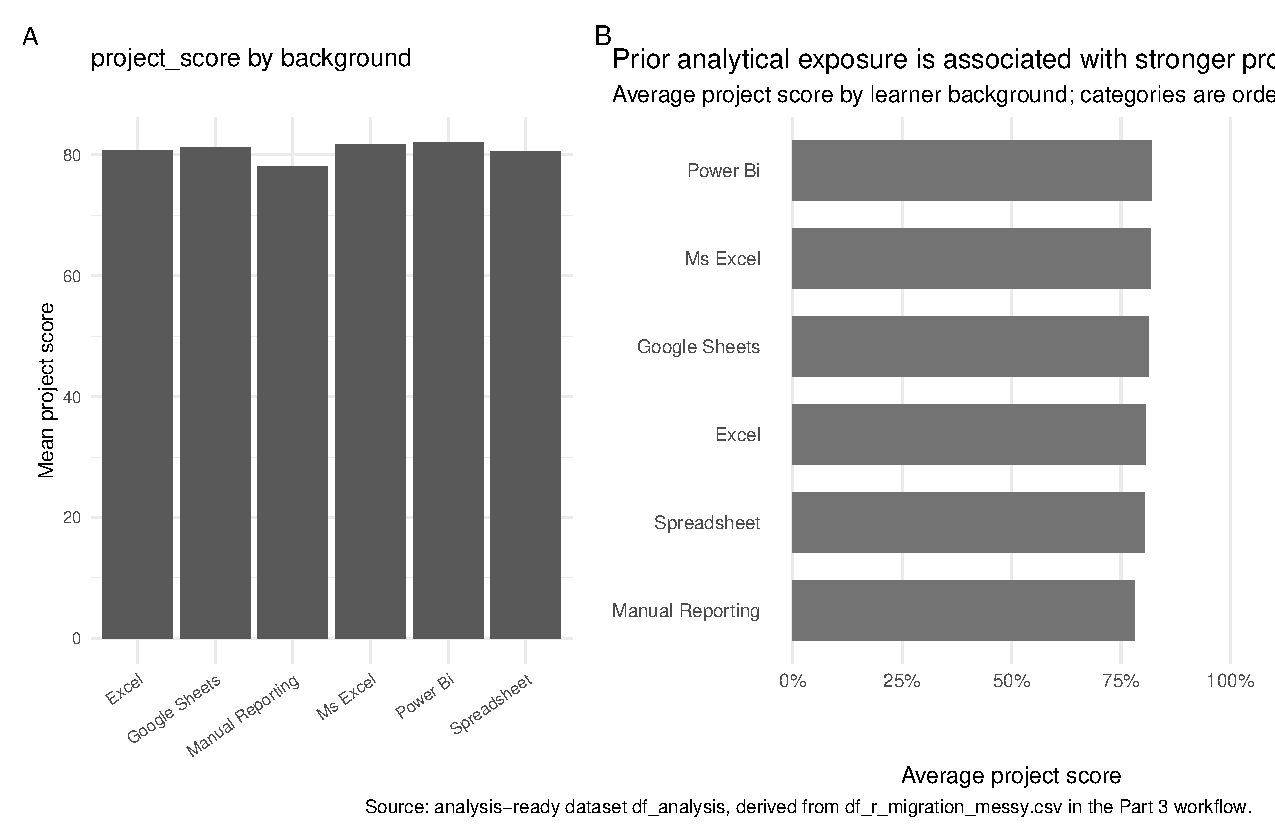
\includegraphics[width=0.9\linewidth,height=\textheight,keepaspectratio,alt={Two bar charts comparing average project score by learner background. The redesigned chart orders backgrounds by score, uses clearer labels, and makes the comparison easier to read.}]{chapters/18-communication-from-plots-to-story_files/figure-pdf/fig-18-1-before-after-redesign-1.pdf}

}

\caption{\label{fig-18-1-before-after-redesign}A Quick Exploratory Bar
Chart Redesigned as An Explanatory Visual.}

\end{figure}%

The code in Listing~\ref{lst-fig-18-1-before-after-redesign} produces
Figure~\ref{fig-18-1-before-after-redesign}.

Notice what changed.

The redesigned plot does not contain more data. It contains more
guidance. The categories are ordered. The title makes the intended
comparison visible. The subtitle tells the reader what has been
summarized. The caption identifies the source. The y-axis uses a scale
that matches the score range. The gridlines are quieter.

This is not cosmetic improvement. It is communicative control.

\section{Visual Hierarchy: Giving the Reader a Scanning
Path}\label{visual-hierarchy-giving-the-reader-a-scanning-path}

A reader does not absorb a plot all at once. The eye lands somewhere
first, then moves. Good visual design creates a scanning path.

In a weak plot, everything competes for attention: title, axes, bars,
gridlines, legend, labels, colours, captions, and annotations. The
reader does not know where to begin.

In a stronger plot, hierarchy is deliberate:

\begin{enumerate}
\def\labelenumi{\arabic{enumi}.}
\tightlist
\item
  The title tells the reader the main point.
\item
  The subtitle explains the analytical frame.
\item
  The main data mark carries the evidence.
\item
  Labels and annotations clarify the important detail.
\item
  Axes support interpretation without dominating.
\item
  The caption gives source and scope information.
\item
  Background elements stay quiet.
\end{enumerate}

Visual hierarchy is created through size, weight, contrast, spacing,
position, and saturation.

\begin{Shaded}
\begin{Highlighting}[]
\NormalTok{tibble}\SpecialCharTok{::}\FunctionTok{tribble}\NormalTok{(}
  \SpecialCharTok{\textasciitilde{}}\StringTok{\textasciigrave{}}\AttributeTok{Design Element}\StringTok{\textasciigrave{}}\NormalTok{, }\SpecialCharTok{\textasciitilde{}}\StringTok{\textasciigrave{}}\AttributeTok{What It Controls}\StringTok{\textasciigrave{}}\NormalTok{, }\SpecialCharTok{\textasciitilde{}}\StringTok{\textasciigrave{}}\AttributeTok{Practical R Move}\StringTok{\textasciigrave{}}\NormalTok{,}
  \StringTok{"Title"}\NormalTok{, }\StringTok{"First interpretive cue"}\NormalTok{, }\StringTok{"Use \textasciigrave{}labs(title = ...)\textasciigrave{} to state the message, not merely the variable names."}\NormalTok{,}
  \StringTok{"Subtitle"}\NormalTok{, }\StringTok{"Analytical context"}\NormalTok{, }\StringTok{"Use \textasciigrave{}labs(subtitle = ...)\textasciigrave{} to explain comparison, period, filter, or summary method."}\NormalTok{,}
  \StringTok{"Colour saturation"}\NormalTok{, }\StringTok{"Attention priority"}\NormalTok{, }\StringTok{"Use stronger colour only for the group or pattern that needs focus."}\NormalTok{,}
  \StringTok{"Line weight"}\NormalTok{, }\StringTok{"Importance of a trend"}\NormalTok{, }\StringTok{"Use \textasciigrave{}linewidth\textasciigrave{} to make focal lines stronger and background lines quieter."}\NormalTok{,}
  \StringTok{"Text size"}\NormalTok{, }\StringTok{"Reading order"}\NormalTok{, }\StringTok{"Use larger title text, moderate axis text, and smaller captions."}\NormalTok{,}
  \StringTok{"Gridlines"}\NormalTok{, }\StringTok{"Reference support"}\NormalTok{, }\StringTok{"Remove minor gridlines and reduce visual noise with \textasciigrave{}theme()\textasciigrave{}."}\NormalTok{,}
  \StringTok{"Spacing"}\NormalTok{, }\StringTok{"Legibility"}\NormalTok{, }\StringTok{"Use \textasciigrave{}coord\_flip()\textasciigrave{}, margins, and uncluttered labels where category names are long."}\NormalTok{,}
  \StringTok{"Caption"}\NormalTok{, }\StringTok{"Source and limitation"}\NormalTok{, }\StringTok{"Use \textasciigrave{}labs(caption = ...)\textasciigrave{} to credit data and clarify scope."}
\NormalTok{) }\SpecialCharTok{\%\textgreater{}\%}
\NormalTok{  knitr}\SpecialCharTok{::}\FunctionTok{kable}\NormalTok{()}
\end{Highlighting}
\end{Shaded}

{

\begin{longtable}[]{@{}
  >{\raggedright\arraybackslash}p{(\linewidth - 4\tabcolsep) * \real{0.1429}}
  >{\raggedright\arraybackslash}p{(\linewidth - 4\tabcolsep) * \real{0.1825}}
  >{\raggedright\arraybackslash}p{(\linewidth - 4\tabcolsep) * \real{0.6746}}@{}}

\caption{\label{tbl-18-2-visual-hierarchy}Practical Ways to Create
Visual Hierarchy in R Plots.}

\tabularnewline

\toprule\noalign{}
\begin{minipage}[b]{\linewidth}\raggedright
Design Element
\end{minipage} & \begin{minipage}[b]{\linewidth}\raggedright
What It Controls
\end{minipage} & \begin{minipage}[b]{\linewidth}\raggedright
Practical R Move
\end{minipage} \\
\midrule\noalign{}
\endhead
\bottomrule\noalign{}
\endlastfoot
Title & First interpretive cue & Use \texttt{labs(title\ =\ ...)} to
state the message, not merely the variable names. \\
Subtitle & Analytical context & Use \texttt{labs(subtitle\ =\ ...)} to
explain comparison, period, filter, or summary method. \\
Colour saturation & Attention priority & Use stronger colour only for
the group or pattern that needs focus. \\
Line weight & Importance of a trend & Use \texttt{linewidth} to make
focal lines stronger and background lines quieter. \\
Text size & Reading order & Use larger title text, moderate axis text,
and smaller captions. \\
Gridlines & Reference support & Remove minor gridlines and reduce visual
noise with \texttt{theme()}. \\
Spacing & Legibility & Use \texttt{coord\_flip()}, margins, and
uncluttered labels where category names are long. \\
Caption & Source and limitation & Use \texttt{labs(caption\ =\ ...)} to
credit data and clarify scope. \\

\end{longtable}

}

Table~\ref{tbl-18-2-visual-hierarchy} gives Leo a compact map of the
design moves that create visual hierarchy.

A useful principle is this:

\begin{quote}
The most important thing should be the easiest thing to find.
\end{quote}

If everything is equally loud, the plot has no hierarchy. If the
important pattern is visually quiet while decorative features are
visually strong, the chart is working against the reader.

\section{Semantic Text Layers: Title, Subtitle, Tag, and
Caption}\label{semantic-text-layers-title-subtitle-tag-and-caption}

In beginner plots, text often appears as a label afterthought. Leo
writes a title because the plot needs a title. He writes a caption
because someone told him captions are professional.

In explanatory visualization, text layers have different jobs.

\begin{Shaded}
\begin{Highlighting}[]
\NormalTok{tibble}\SpecialCharTok{::}\FunctionTok{tribble}\NormalTok{(}
  \SpecialCharTok{\textasciitilde{}}\StringTok{\textasciigrave{}}\AttributeTok{Text Layer}\StringTok{\textasciigrave{}}\NormalTok{, }\SpecialCharTok{\textasciitilde{}}\StringTok{\textasciigrave{}}\AttributeTok{Main Job}\StringTok{\textasciigrave{}}\NormalTok{, }\SpecialCharTok{\textasciitilde{}}\StringTok{\textasciigrave{}}\AttributeTok{Weak Version}\StringTok{\textasciigrave{}}\NormalTok{, }\SpecialCharTok{\textasciitilde{}}\StringTok{\textasciigrave{}}\AttributeTok{Stronger Version}\StringTok{\textasciigrave{}}\NormalTok{,}
  \StringTok{"Title"}\NormalTok{, }\StringTok{"State the main message"}\NormalTok{, }\StringTok{"Project scores"}\NormalTok{, }\StringTok{"Project scores rise with weekly study time"}\NormalTok{,}
  \StringTok{"Subtitle"}\NormalTok{, }\StringTok{"Provide analytical context"}\NormalTok{, }\StringTok{"By week"}\NormalTok{, }\StringTok{"Average scores by learning week; negative study{-}hour records removed during cleaning"}\NormalTok{,}
  \StringTok{"Tag"}\NormalTok{, }\StringTok{"Orient the reader in a sequence"}\NormalTok{, }\StringTok{"Plot 1"}\NormalTok{, }\StringTok{"A"}\NormalTok{,}
  \StringTok{"Axis label"}\NormalTok{, }\StringTok{"Name the measurement clearly"}\NormalTok{, }\StringTok{"score"}\NormalTok{, }\StringTok{"Average project score"}\NormalTok{,}
  \StringTok{"Inline label"}\NormalTok{, }\StringTok{"Identify the focal group near the data"}\NormalTok{, }\StringTok{"Legend only"}\NormalTok{, }\StringTok{"Label the highlighted line directly"}\NormalTok{,}
  \StringTok{"Caption"}\NormalTok{, }\StringTok{"Credit source and clarify scope"}\NormalTok{, }\StringTok{"Data: survey"}\NormalTok{, }\StringTok{"Source: df\_analysis, the analysis{-}ready dataset created in Part 3; values shown after preparation for plotting"}
\NormalTok{) }\SpecialCharTok{\%\textgreater{}\%}
\NormalTok{  knitr}\SpecialCharTok{::}\FunctionTok{kable}\NormalTok{()}
\end{Highlighting}
\end{Shaded}

{

\begin{longtable}[]{@{}
  >{\raggedright\arraybackslash}p{(\linewidth - 6\tabcolsep) * \real{0.0730}}
  >{\raggedright\arraybackslash}p{(\linewidth - 6\tabcolsep) * \real{0.2191}}
  >{\raggedright\arraybackslash}p{(\linewidth - 6\tabcolsep) * \real{0.0843}}
  >{\raggedright\arraybackslash}p{(\linewidth - 6\tabcolsep) * \real{0.6236}}@{}}

\caption{\label{tbl-18-3-semantic-text-layers}The Communication Roles of
Titles, Subtitles, Tags, and Captions.}

\tabularnewline

\toprule\noalign{}
\begin{minipage}[b]{\linewidth}\raggedright
Text Layer
\end{minipage} & \begin{minipage}[b]{\linewidth}\raggedright
Main Job
\end{minipage} & \begin{minipage}[b]{\linewidth}\raggedright
Weak Version
\end{minipage} & \begin{minipage}[b]{\linewidth}\raggedright
Stronger Version
\end{minipage} \\
\midrule\noalign{}
\endhead
\bottomrule\noalign{}
\endlastfoot
Title & State the main message & Project scores & Project scores rise
with weekly study time \\
Subtitle & Provide analytical context & By week & Average scores by
learning week; negative study-hour records removed during cleaning \\
Tag & Orient the reader in a sequence & Plot 1 & A \\
Axis label & Name the measurement clearly & score & Average project
score \\
Inline label & Identify the focal group near the data & Legend only &
Label the highlighted line directly \\
Caption & Credit source and clarify scope & Data: survey & Source:
df\_analysis, the analysis-ready dataset created in Part 3; values shown
after preparation for plotting \\

\end{longtable}

}

Table~\ref{tbl-18-3-semantic-text-layers} separates the communication
jobs of titles, subtitles, tags, axis labels, inline labels, and
captions.

A good title does not need to be sensational. It needs to be useful.

Compare these:

\begin{itemize}
\tightlist
\item
  ``Study Hours and Project Score''
\item
  ``Learners who study more hours tend to record higher project scores''
\end{itemize}

The first title names the variables. The second title tells the reader
what relationship to inspect. It still uses careful language: ``tend
to'' rather than ``prove that.'' It points without overstating.

\begin{tcolorbox}[enhanced jigsaw, arc=.35mm, bottomrule=.15mm, breakable, colback=white, colframe=quarto-callout-tip-color-frame, left=2mm, leftrule=.75mm, opacityback=0, rightrule=.15mm, toprule=.15mm]
\begin{minipage}[t]{5.5mm}
\textcolor{quarto-callout-tip-color}{\faLightbulb}
\end{minipage}%
\begin{minipage}[t]{\textwidth - 5.5mm}

\vspace{-3mm}\textbf{A practical title pattern}\vspace{3mm}

For explanatory plots, Leo can draft titles using this structure:

\textbf{{[}Who or what{]} + {[}does what{]} + {[}under what condition or
comparison{]}.}

Example: \textbf{Learners using project-based study show higher average
project scores.}

\end{minipage}%
\end{tcolorbox}

\section{Typographic Architecture}\label{typographic-architecture}

Typography is not decoration. It is part of the reading system of a
plot.

A professional plot usually has a simple hierarchy:

\begin{itemize}
\tightlist
\item
  title: largest and strongest;
\item
  subtitle: smaller and explanatory;
\item
  axis titles: clear but not dominant;
\item
  axis text: readable;
\item
  annotation: visible at the point of need;
\item
  caption: smaller but still legible.
\end{itemize}

The point is not to use fancy fonts. The point is to make reading
predictable.

R can use system fonts through the graphics device, and packages such as
\texttt{systemfonts} can help identify available fonts. The
\texttt{showtext} package can also help render fonts consistently across
devices, including fonts loaded from local files or online font
services. Those workflows are useful, but they are also
system-dependent. A beginner-facing chapter should therefore teach the
principle without making the project depend on a font that may not exist
on another machine.

\begin{codelisting}

\caption{\label{lst-chapter18-systemfonts-check}Code for Inspecting
Available System Fonts}

\centering{

\begin{Shaded}
\begin{Highlighting}[]
\CommentTok{\# Optional: inspect fonts available on your system.}
\CommentTok{\# This requires the systemfonts package.}

\FunctionTok{library}\NormalTok{(systemfonts)}

\NormalTok{systemfonts}\SpecialCharTok{::}\FunctionTok{system\_fonts}\NormalTok{() }\SpecialCharTok{|\textgreater{}}
\NormalTok{  dplyr}\SpecialCharTok{::}\FunctionTok{select}\NormalTok{(family, style, path) }\SpecialCharTok{|\textgreater{}}
\NormalTok{  dplyr}\SpecialCharTok{::}\FunctionTok{distinct}\NormalTok{(family, style, }\AttributeTok{.keep\_all =} \ConstantTok{TRUE}\NormalTok{) }\SpecialCharTok{|\textgreater{}}
\NormalTok{  dplyr}\SpecialCharTok{::}\FunctionTok{arrange}\NormalTok{(family)}
\end{Highlighting}
\end{Shaded}

}

\end{codelisting}%

The optional code in Listing~\ref{lst-chapter18-systemfonts-check} shows
how Leo can inspect available system fonts before choosing a font family
for a plot.

\begin{codelisting}

\caption{\label{lst-chapter18-safe-typography-example}Code for a Safe
Typography Pattern That Does Not Require a Special Font}

\centering{

\begin{Shaded}
\begin{Highlighting}[]
\CommentTok{\# Safe typography pattern.}
\CommentTok{\# Use a generic font family that should exist across systems.}

\NormalTok{base\_family }\OtherTok{\textless{}{-}} \StringTok{"sans"}

\FunctionTok{ggplot}\NormalTok{(df\_story, }\FunctionTok{aes}\NormalTok{(}\AttributeTok{x =}\NormalTok{ study\_hours, }\AttributeTok{y =}\NormalTok{ project\_score)) }\SpecialCharTok{+}
  \FunctionTok{geom\_point}\NormalTok{(}\AttributeTok{alpha =} \FloatTok{0.35}\NormalTok{) }\SpecialCharTok{+}
  \FunctionTok{geom\_smooth}\NormalTok{(}\AttributeTok{method =} \StringTok{"lm"}\NormalTok{, }\AttributeTok{se =} \ConstantTok{FALSE}\NormalTok{) }\SpecialCharTok{+}
  \FunctionTok{labs}\NormalTok{(}
    \AttributeTok{title =} \StringTok{"Study time and project performance move together"}\NormalTok{,}
    \AttributeTok{subtitle =} \StringTok{"A simple linear smoother helps the reader see the overall direction."}\NormalTok{,}
    \AttributeTok{x =} \StringTok{"Weekly study hours"}\NormalTok{,}
    \AttributeTok{y =} \StringTok{"Project score"}\NormalTok{,}
    \AttributeTok{caption =}\NormalTok{ chapter18\_caption\_source}
\NormalTok{  ) }\SpecialCharTok{+}
  \FunctionTok{theme\_minimal}\NormalTok{(}\AttributeTok{base\_family =}\NormalTok{ base\_family, }\AttributeTok{base\_size =} \DecValTok{11}\NormalTok{) }\SpecialCharTok{+}
  \FunctionTok{theme}\NormalTok{(}
    \AttributeTok{plot.title =} \FunctionTok{element\_text}\NormalTok{(}\AttributeTok{size =} \DecValTok{15}\NormalTok{, }\AttributeTok{face =} \StringTok{"bold"}\NormalTok{),}
    \AttributeTok{plot.subtitle =} \FunctionTok{element\_text}\NormalTok{(}\AttributeTok{size =} \DecValTok{11}\NormalTok{),}
    \AttributeTok{axis.title =} \FunctionTok{element\_text}\NormalTok{(}\AttributeTok{size =} \DecValTok{10}\NormalTok{),}
    \AttributeTok{plot.caption =} \FunctionTok{element\_text}\NormalTok{(}\AttributeTok{size =} \DecValTok{8}\NormalTok{)}
\NormalTok{  )}
\end{Highlighting}
\end{Shaded}

}

\end{codelisting}%

\begin{figure}[H]

\centering{

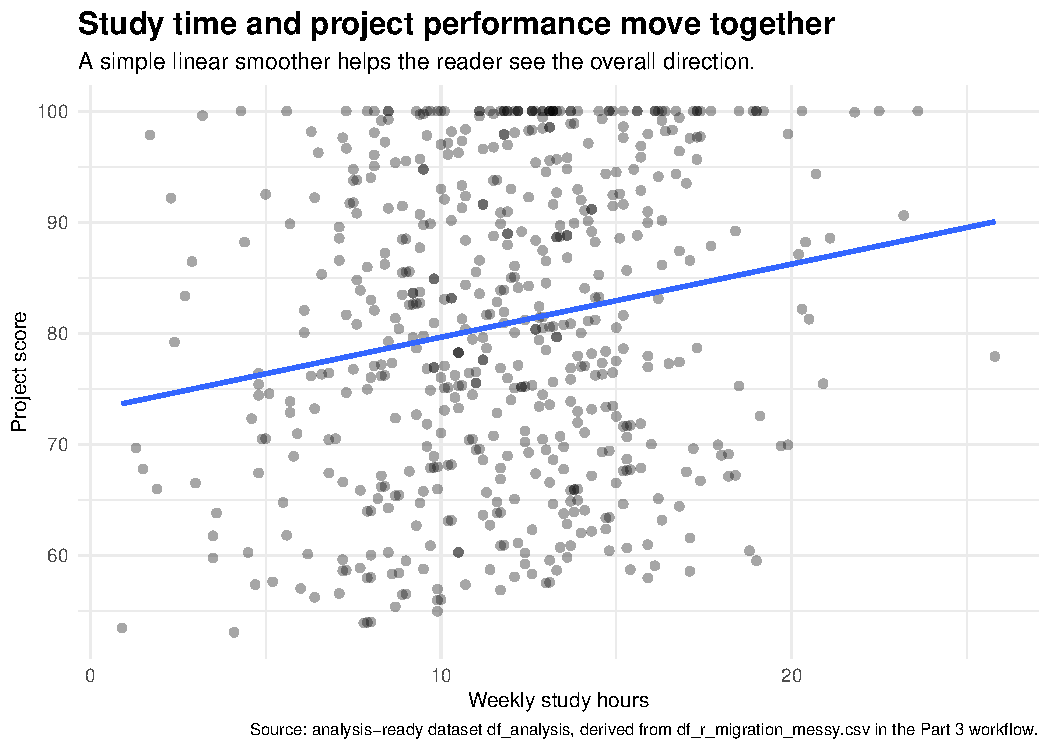
\includegraphics[width=0.9\linewidth,height=\textheight,keepaspectratio,alt={A scatter plot of weekly study hours and project score with a linear trend line and controlled title, subtitle, axis, and caption text sizes.}]{chapters/18-communication-from-plots-to-story_files/figure-pdf/fig-18-safe-typography-example-1.pdf}

}

\caption{\label{fig-18-safe-typography-example}A Safe Typography
Structure Using a Generic Sans Font}

\end{figure}%

The code in Listing~\ref{lst-chapter18-safe-typography-example} produces
Figure~\ref{fig-18-safe-typography-example}.

The key lesson is not ``always use this font.'' The key lesson is:

\begin{quote}
Set a text system deliberately.
\end{quote}

A plot that changes fonts accidentally across devices can look less
polished and may even render labels differently. This matters when a
figure moves from RStudio to slides, Word documents, PDFs, journal
manuscripts, or web pages.

\section{\texorpdfstring{Rich Text Formatting with
\texttt{ggtext}}{Rich Text Formatting with ggtext}}\label{rich-text-formatting-with-ggtext}

Sometimes plain text is not enough. Leo may want part of a title to be
bold, part of a subtitle to be coloured, or a caption to contain a small
emphasis cue. The \texttt{ggtext} package makes this possible by
allowing Markdown and limited HTML-style formatting in plot text
elements through elements such as \texttt{element\_markdown()}.

This should be used with restraint. Rich text is useful when it
clarifies structure. It becomes noise when it merely decorates.

\begin{codelisting}

\caption{\label{lst-fig-18-2-rich-text-labels}Code for Rich Text Labels
That Clarify the Message}

\centering{

\begin{Shaded}
\begin{Highlighting}[]
\NormalTok{rich\_text\_theme }\OtherTok{\textless{}{-}} \FunctionTok{theme\_minimal}\NormalTok{(}\AttributeTok{base\_size =} \DecValTok{11}\NormalTok{) }\SpecialCharTok{+}
  \FunctionTok{theme}\NormalTok{(}
    \AttributeTok{panel.grid.minor =} \FunctionTok{element\_blank}\NormalTok{(),}
    \AttributeTok{plot.title.position =} \StringTok{"plot"}\NormalTok{,}
    \AttributeTok{plot.caption.position =} \StringTok{"plot"}
\NormalTok{  )}

\ControlFlowTok{if}\NormalTok{ (}\FunctionTok{chapter18\_has\_pkg}\NormalTok{(}\StringTok{"ggtext"}\NormalTok{)) \{}
\NormalTok{  rich\_text\_theme }\OtherTok{\textless{}{-}}\NormalTok{ rich\_text\_theme }\SpecialCharTok{+}
    \FunctionTok{theme}\NormalTok{(}
      \AttributeTok{plot.title =}\NormalTok{ ggtext}\SpecialCharTok{::}\FunctionTok{element\_markdown}\NormalTok{(}\AttributeTok{face =} \StringTok{"bold"}\NormalTok{),}
      \AttributeTok{plot.subtitle =}\NormalTok{ ggtext}\SpecialCharTok{::}\FunctionTok{element\_markdown}\NormalTok{(),}
      \AttributeTok{plot.caption =}\NormalTok{ ggtext}\SpecialCharTok{::}\FunctionTok{element\_markdown}\NormalTok{(}\AttributeTok{size =} \DecValTok{8}\NormalTok{)}
\NormalTok{    )}

\NormalTok{  plot\_title }\OtherTok{\textless{}{-}} \StringTok{"**Study time** and **project score** move in the same direction"}
\NormalTok{  plot\_subtitle }\OtherTok{\textless{}{-}} \StringTok{"Each point represents a learner{-}week record; the smooth line summarizes the broad pattern."}
\NormalTok{  plot\_caption }\OtherTok{\textless{}{-}} \FunctionTok{paste0}\NormalTok{(}\StringTok{"**Source:** "}\NormalTok{, chapter18\_caption\_source)}
\NormalTok{\} }\ControlFlowTok{else}\NormalTok{ \{}
\NormalTok{  plot\_title }\OtherTok{\textless{}{-}} \StringTok{"Study time and project score move in the same direction"}
\NormalTok{  plot\_subtitle }\OtherTok{\textless{}{-}} \StringTok{"Each point represents a learner{-}week record; the smooth line summarizes the broad pattern."}
\NormalTok{  plot\_caption }\OtherTok{\textless{}{-}}\NormalTok{ chapter18\_caption\_source}
\NormalTok{\}}

\FunctionTok{ggplot}\NormalTok{(df\_story, }\FunctionTok{aes}\NormalTok{(}\AttributeTok{x =}\NormalTok{ study\_hours, }\AttributeTok{y =}\NormalTok{ project\_score)) }\SpecialCharTok{+}
  \FunctionTok{geom\_point}\NormalTok{(}\AttributeTok{alpha =} \FloatTok{0.28}\NormalTok{, }\AttributeTok{colour =} \StringTok{"grey45"}\NormalTok{) }\SpecialCharTok{+}
  \FunctionTok{geom\_smooth}\NormalTok{(}\AttributeTok{method =} \StringTok{"lm"}\NormalTok{, }\AttributeTok{se =} \ConstantTok{FALSE}\NormalTok{, }\AttributeTok{linewidth =} \FloatTok{0.9}\NormalTok{, }\AttributeTok{colour =} \StringTok{"black"}\NormalTok{) }\SpecialCharTok{+}
  \FunctionTok{scale\_x\_continuous}\NormalTok{(}\AttributeTok{labels =}\NormalTok{ scales}\SpecialCharTok{::}\FunctionTok{label\_number}\NormalTok{(}\AttributeTok{suffix =} \StringTok{" hrs"}\NormalTok{)) }\SpecialCharTok{+}
  \FunctionTok{scale\_y\_continuous}\NormalTok{(}\AttributeTok{limits =} \FunctionTok{c}\NormalTok{(}\DecValTok{0}\NormalTok{, }\DecValTok{100}\NormalTok{), }\AttributeTok{labels =}\NormalTok{ scales}\SpecialCharTok{::}\FunctionTok{label\_number}\NormalTok{(}\AttributeTok{suffix =} \StringTok{"\%"}\NormalTok{)) }\SpecialCharTok{+}
  \FunctionTok{labs}\NormalTok{(}
    \AttributeTok{title =}\NormalTok{ plot\_title,}
    \AttributeTok{subtitle =}\NormalTok{ plot\_subtitle,}
    \AttributeTok{x =} \StringTok{"Weekly study hours"}\NormalTok{,}
    \AttributeTok{y =} \StringTok{"Project score"}\NormalTok{,}
    \AttributeTok{caption =}\NormalTok{ plot\_caption}
\NormalTok{  ) }\SpecialCharTok{+}
\NormalTok{  rich\_text\_theme}
\end{Highlighting}
\end{Shaded}

}

\end{codelisting}%

\begin{figure}[H]

\centering{

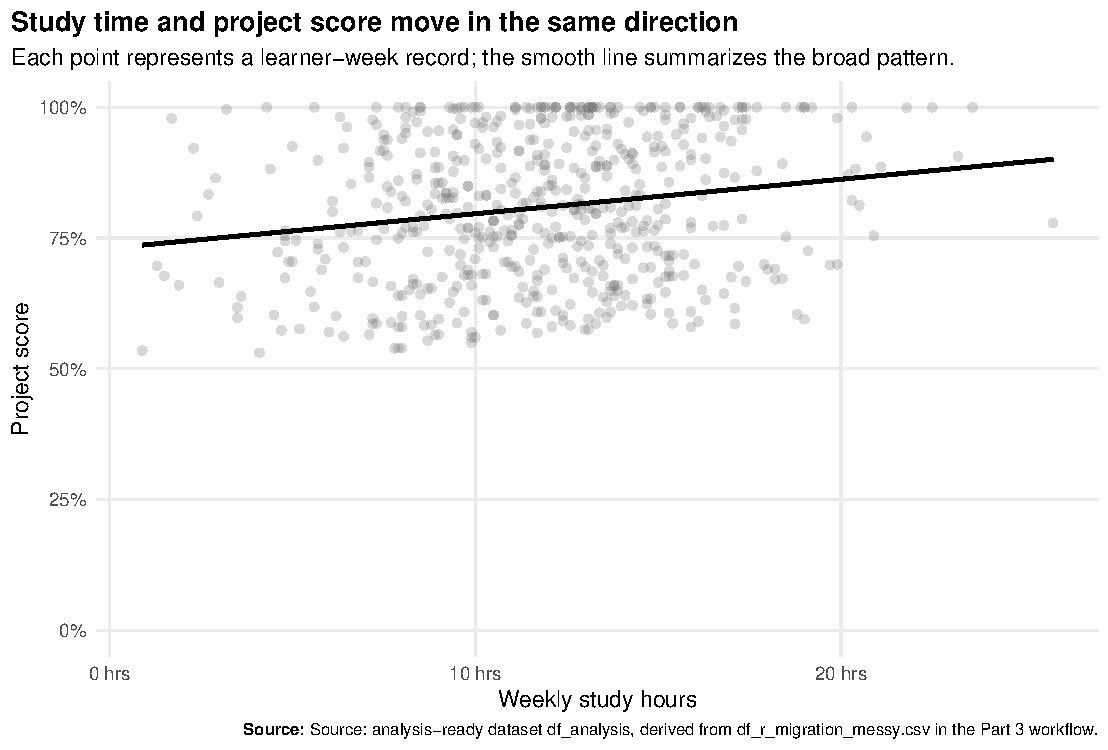
\includegraphics[width=0.9\linewidth,height=\textheight,keepaspectratio,alt={A scatter plot of weekly study hours and project score with a title that emphasizes study time and project score. A trend line shows the general upward relationship.}]{chapters/18-communication-from-plots-to-story_files/figure-pdf/fig-18-2-rich-text-labels-1.pdf}

}

\caption{\label{fig-18-2-rich-text-labels}Rich Text Labels Can Add
Emphasis When They Clarify the Message.}

\end{figure}%

The code in Listing~\ref{lst-fig-18-2-rich-text-labels} produces
Figure~\ref{fig-18-2-rich-text-labels}.

If \texttt{ggtext} is installed, the title and caption can interpret
Markdown-style emphasis. If it is not installed, the plot still renders
with plain text. That is a safe pattern: optional enhancement, not
fragile dependency.

\begin{tcolorbox}[enhanced jigsaw, arc=.35mm, bottomrule=.15mm, breakable, colback=white, colframe=quarto-callout-warning-color-frame, left=2mm, leftrule=.75mm, opacityback=0, rightrule=.15mm, toprule=.15mm]
\begin{minipage}[t]{5.5mm}
\textcolor{quarto-callout-warning-color}{\faExclamationTriangle}
\end{minipage}%
\begin{minipage}[t]{\textwidth - 5.5mm}

\vspace{-3mm}\textbf{Use rich text for meaning, not decoration}\vspace{3mm}

Bold text, colour, and HTML-like styling can help guide attention. But
if every label is styled, no label is special. Use rich text where it
helps the reader understand the hierarchy of the message.

\end{minipage}%
\end{tcolorbox}

\section{Dynamic Data Highlighting}\label{dynamic-data-highlighting}

One of the strongest explanatory moves is to reduce background noise
while preserving context.

Suppose Leo wants to show how one preferred learning mode performs
across weeks. He could plot only that group, but then the reader loses
the comparison. He could plot all groups equally, but then the focal
pattern may disappear.

Highlighting solves the problem: keep the context, reduce its visual
weight, and bring the focal group forward.

The \texttt{gghighlight} package can automate this pattern for many
plots. The next figure uses \texttt{gghighlight} when available and
falls back to a manual highlighting approach when it is not.

\begin{codelisting}

\caption{\label{lst-fig-18-3-dynamic-highlight}Code for Dynamic
Highlighting of One Focal Learning Mode}

\centering{

\begin{Shaded}
\begin{Highlighting}[]
\NormalTok{weekly\_mode }\OtherTok{\textless{}{-}}\NormalTok{ df\_story }\SpecialCharTok{\%\textgreater{}\%}
  \FunctionTok{filter}\NormalTok{(}\SpecialCharTok{!}\FunctionTok{is.na}\NormalTok{(preferred\_learning\_mode), }\SpecialCharTok{!}\FunctionTok{is.na}\NormalTok{(week)) }\SpecialCharTok{\%\textgreater{}\%}
  \FunctionTok{group\_by}\NormalTok{(preferred\_learning\_mode, week) }\SpecialCharTok{\%\textgreater{}\%}
  \FunctionTok{summarise}\NormalTok{(}
    \AttributeTok{mean\_project =} \FunctionTok{mean}\NormalTok{(project\_score, }\AttributeTok{na.rm =} \ConstantTok{TRUE}\NormalTok{),}
    \AttributeTok{learners =} \FunctionTok{n}\NormalTok{(),}
    \AttributeTok{.groups =} \StringTok{"drop"}
\NormalTok{  ) }\SpecialCharTok{\%\textgreater{}\%}
  \FunctionTok{filter}\NormalTok{(learners }\SpecialCharTok{\textgreater{}=} \DecValTok{2}\NormalTok{)}

\NormalTok{target\_mode }\OtherTok{\textless{}{-}}\NormalTok{ weekly\_mode }\SpecialCharTok{\%\textgreater{}\%}
  \FunctionTok{group\_by}\NormalTok{(preferred\_learning\_mode) }\SpecialCharTok{\%\textgreater{}\%}
  \FunctionTok{summarise}\NormalTok{(}\AttributeTok{last\_score =}\NormalTok{ mean\_project[}\FunctionTok{which.max}\NormalTok{(week)], }\AttributeTok{.groups =} \StringTok{"drop"}\NormalTok{) }\SpecialCharTok{\%\textgreater{}\%}
  \FunctionTok{arrange}\NormalTok{(}\FunctionTok{desc}\NormalTok{(last\_score)) }\SpecialCharTok{\%\textgreater{}\%}
  \FunctionTok{slice}\NormalTok{(}\DecValTok{1}\NormalTok{) }\SpecialCharTok{\%\textgreater{}\%}
  \FunctionTok{pull}\NormalTok{(preferred\_learning\_mode)}

\NormalTok{highlight\_plot }\OtherTok{\textless{}{-}} \FunctionTok{ggplot}\NormalTok{(}
\NormalTok{  weekly\_mode,}
  \FunctionTok{aes}\NormalTok{(}\AttributeTok{x =}\NormalTok{ week, }\AttributeTok{y =}\NormalTok{ mean\_project, }\AttributeTok{group =}\NormalTok{ preferred\_learning\_mode)}
\NormalTok{) }\SpecialCharTok{+}
  \FunctionTok{geom\_line}\NormalTok{(}\FunctionTok{aes}\NormalTok{(}\AttributeTok{colour =}\NormalTok{ preferred\_learning\_mode), }\AttributeTok{linewidth =} \FloatTok{0.8}\NormalTok{, }\AttributeTok{alpha =} \FloatTok{0.75}\NormalTok{) }\SpecialCharTok{+}
  \FunctionTok{geom\_point}\NormalTok{(}\FunctionTok{aes}\NormalTok{(}\AttributeTok{colour =}\NormalTok{ preferred\_learning\_mode), }\AttributeTok{size =} \FloatTok{1.8}\NormalTok{, }\AttributeTok{alpha =} \FloatTok{0.75}\NormalTok{) }\SpecialCharTok{+}
  \FunctionTok{scale\_x\_continuous}\NormalTok{(}\AttributeTok{breaks =} \FunctionTok{sort}\NormalTok{(}\FunctionTok{unique}\NormalTok{(weekly\_mode}\SpecialCharTok{$}\NormalTok{week))) }\SpecialCharTok{+}
  \FunctionTok{scale\_y\_continuous}\NormalTok{(}\AttributeTok{limits =} \FunctionTok{c}\NormalTok{(}\DecValTok{0}\NormalTok{, }\DecValTok{100}\NormalTok{), }\AttributeTok{labels =}\NormalTok{ scales}\SpecialCharTok{::}\FunctionTok{label\_number}\NormalTok{(}\AttributeTok{suffix =} \StringTok{"\%"}\NormalTok{)) }\SpecialCharTok{+}
  \FunctionTok{labs}\NormalTok{(}
    \AttributeTok{title =} \FunctionTok{paste0}\NormalTok{(target\_mode, }\StringTok{" stands out in the weekly project{-}score trend"}\NormalTok{),}
    \AttributeTok{subtitle =} \StringTok{"Background lines remain visible so the highlighted trend can be read in context."}\NormalTok{,}
    \AttributeTok{x =} \StringTok{"Learning week"}\NormalTok{,}
    \AttributeTok{y =} \StringTok{"Average project score"}\NormalTok{,}
    \AttributeTok{caption =}\NormalTok{ chapter18\_caption\_source}
\NormalTok{  ) }\SpecialCharTok{+}
  \FunctionTok{theme\_minimal}\NormalTok{(}\AttributeTok{base\_size =} \DecValTok{11}\NormalTok{) }\SpecialCharTok{+}
  \FunctionTok{theme}\NormalTok{(}
    \AttributeTok{legend.position =} \StringTok{"none"}\NormalTok{,}
    \AttributeTok{panel.grid.minor =} \FunctionTok{element\_blank}\NormalTok{(),}
    \AttributeTok{plot.title.position =} \StringTok{"plot"}\NormalTok{,}
    \AttributeTok{plot.caption.position =} \StringTok{"plot"}
\NormalTok{  )}

\ControlFlowTok{if}\NormalTok{ (}\FunctionTok{chapter18\_has\_pkg}\NormalTok{(}\StringTok{"gghighlight"}\NormalTok{)) \{}
\NormalTok{  highlight\_plot }\SpecialCharTok{+}
\NormalTok{    gghighlight}\SpecialCharTok{::}\FunctionTok{gghighlight}\NormalTok{(}
\NormalTok{      preferred\_learning\_mode }\SpecialCharTok{==}\NormalTok{ target\_mode,}
      \AttributeTok{unhighlighted\_params =} \FunctionTok{list}\NormalTok{(}\AttributeTok{colour =} \StringTok{"grey80"}\NormalTok{, }\AttributeTok{linewidth =} \FloatTok{0.5}\NormalTok{, }\AttributeTok{alpha =} \FloatTok{0.6}\NormalTok{),}
      \AttributeTok{use\_direct\_label =} \ConstantTok{FALSE}
\NormalTok{    )}
\NormalTok{\} }\ControlFlowTok{else}\NormalTok{ \{}
\NormalTok{  weekly\_mode }\SpecialCharTok{\%\textgreater{}\%}
    \FunctionTok{mutate}\NormalTok{(}\AttributeTok{is\_target =}\NormalTok{ preferred\_learning\_mode }\SpecialCharTok{==}\NormalTok{ target\_mode) }\SpecialCharTok{\%\textgreater{}\%}
    \FunctionTok{ggplot}\NormalTok{(}\FunctionTok{aes}\NormalTok{(}\AttributeTok{x =}\NormalTok{ week, }\AttributeTok{y =}\NormalTok{ mean\_project, }\AttributeTok{group =}\NormalTok{ preferred\_learning\_mode)) }\SpecialCharTok{+}
    \FunctionTok{geom\_line}\NormalTok{(}
      \FunctionTok{aes}\NormalTok{(}\AttributeTok{linewidth =}\NormalTok{ is\_target, }\AttributeTok{alpha =}\NormalTok{ is\_target),}
      \AttributeTok{colour =} \StringTok{"grey45"}
\NormalTok{    ) }\SpecialCharTok{+}
    \FunctionTok{geom\_point}\NormalTok{(}
      \FunctionTok{aes}\NormalTok{(}\AttributeTok{size =}\NormalTok{ is\_target, }\AttributeTok{alpha =}\NormalTok{ is\_target),}
      \AttributeTok{colour =} \StringTok{"grey30"}
\NormalTok{    ) }\SpecialCharTok{+}
    \FunctionTok{scale\_linewidth\_manual}\NormalTok{(}\AttributeTok{values =} \FunctionTok{c}\NormalTok{(}\StringTok{\textasciigrave{}}\AttributeTok{FALSE}\StringTok{\textasciigrave{}} \OtherTok{=} \FloatTok{0.45}\NormalTok{, }\StringTok{\textasciigrave{}}\AttributeTok{TRUE}\StringTok{\textasciigrave{}} \OtherTok{=} \FloatTok{1.1}\NormalTok{), }\AttributeTok{guide =} \StringTok{"none"}\NormalTok{) }\SpecialCharTok{+}
    \FunctionTok{scale\_size\_manual}\NormalTok{(}\AttributeTok{values =} \FunctionTok{c}\NormalTok{(}\StringTok{\textasciigrave{}}\AttributeTok{FALSE}\StringTok{\textasciigrave{}} \OtherTok{=} \FloatTok{1.2}\NormalTok{, }\StringTok{\textasciigrave{}}\AttributeTok{TRUE}\StringTok{\textasciigrave{}} \OtherTok{=} \FloatTok{2.2}\NormalTok{), }\AttributeTok{guide =} \StringTok{"none"}\NormalTok{) }\SpecialCharTok{+}
    \FunctionTok{scale\_alpha\_manual}\NormalTok{(}\AttributeTok{values =} \FunctionTok{c}\NormalTok{(}\StringTok{\textasciigrave{}}\AttributeTok{FALSE}\StringTok{\textasciigrave{}} \OtherTok{=} \FloatTok{0.35}\NormalTok{, }\StringTok{\textasciigrave{}}\AttributeTok{TRUE}\StringTok{\textasciigrave{}} \OtherTok{=} \DecValTok{1}\NormalTok{), }\AttributeTok{guide =} \StringTok{"none"}\NormalTok{) }\SpecialCharTok{+}
    \FunctionTok{scale\_x\_continuous}\NormalTok{(}\AttributeTok{breaks =} \FunctionTok{sort}\NormalTok{(}\FunctionTok{unique}\NormalTok{(weekly\_mode}\SpecialCharTok{$}\NormalTok{week))) }\SpecialCharTok{+}
    \FunctionTok{scale\_y\_continuous}\NormalTok{(}\AttributeTok{limits =} \FunctionTok{c}\NormalTok{(}\DecValTok{0}\NormalTok{, }\DecValTok{100}\NormalTok{), }\AttributeTok{labels =}\NormalTok{ scales}\SpecialCharTok{::}\FunctionTok{label\_number}\NormalTok{(}\AttributeTok{suffix =} \StringTok{"\%"}\NormalTok{)) }\SpecialCharTok{+}
    \FunctionTok{labs}\NormalTok{(}
      \AttributeTok{title =} \FunctionTok{paste0}\NormalTok{(target\_mode, }\StringTok{" stands out in the weekly project{-}score trend"}\NormalTok{),}
      \AttributeTok{subtitle =} \StringTok{"Background lines remain visible so the highlighted trend can be read in context."}\NormalTok{,}
      \AttributeTok{x =} \StringTok{"Learning week"}\NormalTok{,}
      \AttributeTok{y =} \StringTok{"Average project score"}\NormalTok{,}
      \AttributeTok{caption =}\NormalTok{ chapter18\_caption\_source}
\NormalTok{    ) }\SpecialCharTok{+}
    \FunctionTok{theme\_minimal}\NormalTok{(}\AttributeTok{base\_size =} \DecValTok{11}\NormalTok{) }\SpecialCharTok{+}
    \FunctionTok{theme}\NormalTok{(}
      \AttributeTok{panel.grid.minor =} \FunctionTok{element\_blank}\NormalTok{(),}
      \AttributeTok{plot.title.position =} \StringTok{"plot"}\NormalTok{,}
      \AttributeTok{plot.caption.position =} \StringTok{"plot"}
\NormalTok{    )}
\NormalTok{\}}
\end{Highlighting}
\end{Shaded}

}

\end{codelisting}%

\begin{figure}[H]

\centering{

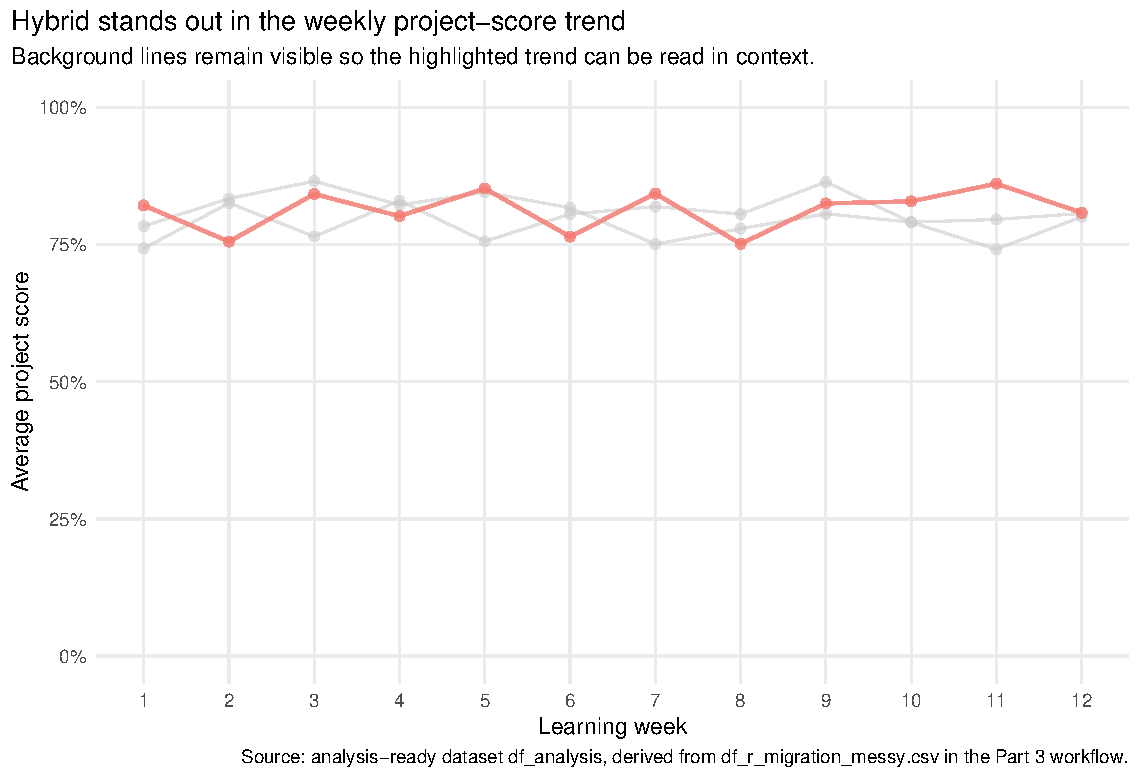
\includegraphics[width=0.9\linewidth,height=\textheight,keepaspectratio,alt={A line chart showing average project score across weeks for preferred learning modes. One learning mode is emphasized while the other lines remain in the background.}]{chapters/18-communication-from-plots-to-story_files/figure-pdf/fig-18-3-dynamic-highlight-1.pdf}

}

\caption{\label{fig-18-3-dynamic-highlight}Dynamic Highlighting Keeps
the Comparison Visible While Directing Attention to One Focal Learning
Mode.}

\end{figure}%

The code in Listing~\ref{lst-fig-18-3-dynamic-highlight} produces
Figure~\ref{fig-18-3-dynamic-highlight}.

This is an important design habit. Leo should not delete context unless
there is a reason. Often, he should quiet the context and foreground the
evidence that answers the question.

\section{Direct Visual Annotation}\label{direct-visual-annotation}

Legends are useful when they are simple. But when a plot has only one or
two important groups, a detached legend may force the reader's eye to
travel back and forth.

Direct annotation places the label close to the data. It reduces
decoding.

The next figure labels the focal trend at the end of the line. If
\texttt{ggrepel} is available, the label uses collision-aware placement.
If not, the plot still uses a plain \texttt{geom\_text()} fallback.

\begin{codelisting}

\caption{\label{lst-fig-18-4-direct-annotation}Code for Direct
Annotation of a Focal Trend}

\centering{

\begin{Shaded}
\begin{Highlighting}[]
\NormalTok{annotated\_weekly }\OtherTok{\textless{}{-}}\NormalTok{ weekly\_mode }\SpecialCharTok{\%\textgreater{}\%}
  \FunctionTok{mutate}\NormalTok{(}\AttributeTok{is\_target =}\NormalTok{ preferred\_learning\_mode }\SpecialCharTok{==}\NormalTok{ target\_mode)}

\NormalTok{last\_label }\OtherTok{\textless{}{-}}\NormalTok{ annotated\_weekly }\SpecialCharTok{\%\textgreater{}\%}
  \FunctionTok{filter}\NormalTok{(is\_target) }\SpecialCharTok{\%\textgreater{}\%}
  \FunctionTok{slice\_max}\NormalTok{(week, }\AttributeTok{n =} \DecValTok{1}\NormalTok{, }\AttributeTok{with\_ties =} \ConstantTok{FALSE}\NormalTok{)}

\NormalTok{annotation\_plot }\OtherTok{\textless{}{-}} \FunctionTok{ggplot}\NormalTok{(}
\NormalTok{  annotated\_weekly,}
  \FunctionTok{aes}\NormalTok{(}\AttributeTok{x =}\NormalTok{ week, }\AttributeTok{y =}\NormalTok{ mean\_project, }\AttributeTok{group =}\NormalTok{ preferred\_learning\_mode)}
\NormalTok{) }\SpecialCharTok{+}
  \FunctionTok{geom\_line}\NormalTok{(}
    \AttributeTok{data =}\NormalTok{ annotated\_weekly }\SpecialCharTok{\%\textgreater{}\%} \FunctionTok{filter}\NormalTok{(}\SpecialCharTok{!}\NormalTok{is\_target),}
    \AttributeTok{colour =} \StringTok{"grey78"}\NormalTok{,}
    \AttributeTok{linewidth =} \FloatTok{0.55}
\NormalTok{  ) }\SpecialCharTok{+}
  \FunctionTok{geom\_line}\NormalTok{(}
    \AttributeTok{data =}\NormalTok{ annotated\_weekly }\SpecialCharTok{\%\textgreater{}\%} \FunctionTok{filter}\NormalTok{(is\_target),}
    \AttributeTok{colour =} \StringTok{"black"}\NormalTok{,}
    \AttributeTok{linewidth =} \FloatTok{1.1}
\NormalTok{  ) }\SpecialCharTok{+}
  \FunctionTok{geom\_point}\NormalTok{(}
    \AttributeTok{data =}\NormalTok{ annotated\_weekly }\SpecialCharTok{\%\textgreater{}\%} \FunctionTok{filter}\NormalTok{(is\_target),}
    \AttributeTok{colour =} \StringTok{"black"}\NormalTok{,}
    \AttributeTok{size =} \DecValTok{2}
\NormalTok{  ) }\SpecialCharTok{+}
  \FunctionTok{scale\_x\_continuous}\NormalTok{(}
    \AttributeTok{breaks =} \FunctionTok{sort}\NormalTok{(}\FunctionTok{unique}\NormalTok{(weekly\_mode}\SpecialCharTok{$}\NormalTok{week)),}
    \AttributeTok{expand =} \FunctionTok{expansion}\NormalTok{(}\AttributeTok{mult =} \FunctionTok{c}\NormalTok{(}\FloatTok{0.02}\NormalTok{, }\FloatTok{0.16}\NormalTok{))}
\NormalTok{  ) }\SpecialCharTok{+}
  \FunctionTok{scale\_y\_continuous}\NormalTok{(}\AttributeTok{limits =} \FunctionTok{c}\NormalTok{(}\DecValTok{0}\NormalTok{, }\DecValTok{100}\NormalTok{), }\AttributeTok{labels =}\NormalTok{ scales}\SpecialCharTok{::}\FunctionTok{label\_number}\NormalTok{(}\AttributeTok{suffix =} \StringTok{"\%"}\NormalTok{)) }\SpecialCharTok{+}
  \FunctionTok{coord\_cartesian}\NormalTok{(}\AttributeTok{clip =} \StringTok{"off"}\NormalTok{) }\SpecialCharTok{+}
  \FunctionTok{labs}\NormalTok{(}
    \AttributeTok{title =} \StringTok{"The focal trend is easier to read when the label moves to the line"}\NormalTok{,}
    \AttributeTok{subtitle =} \StringTok{"Direct annotation reduces the back{-}and{-}forth movement required by a separate legend."}\NormalTok{,}
    \AttributeTok{x =} \StringTok{"Learning week"}\NormalTok{,}
    \AttributeTok{y =} \StringTok{"Average project score"}\NormalTok{,}
    \AttributeTok{caption =}\NormalTok{ chapter18\_caption\_source}
\NormalTok{  ) }\SpecialCharTok{+}
  \FunctionTok{theme\_minimal}\NormalTok{(}\AttributeTok{base\_size =} \DecValTok{11}\NormalTok{) }\SpecialCharTok{+}
  \FunctionTok{theme}\NormalTok{(}
    \AttributeTok{panel.grid.minor =} \FunctionTok{element\_blank}\NormalTok{(),}
    \AttributeTok{plot.margin =} \FunctionTok{margin}\NormalTok{(}\FloatTok{5.5}\NormalTok{, }\DecValTok{45}\NormalTok{, }\FloatTok{5.5}\NormalTok{, }\FloatTok{5.5}\NormalTok{),}
    \AttributeTok{plot.title.position =} \StringTok{"plot"}\NormalTok{,}
    \AttributeTok{plot.caption.position =} \StringTok{"plot"}
\NormalTok{  )}

\ControlFlowTok{if}\NormalTok{ (}\FunctionTok{chapter18\_has\_pkg}\NormalTok{(}\StringTok{"ggrepel"}\NormalTok{)) \{}
\NormalTok{  annotation\_plot }\SpecialCharTok{+}
\NormalTok{    ggrepel}\SpecialCharTok{::}\FunctionTok{geom\_text\_repel}\NormalTok{(}
      \AttributeTok{data =}\NormalTok{ last\_label,}
      \FunctionTok{aes}\NormalTok{(}\AttributeTok{label =}\NormalTok{ preferred\_learning\_mode),}
      \AttributeTok{nudge\_x =} \FloatTok{0.5}\NormalTok{,}
      \AttributeTok{direction =} \StringTok{"y"}\NormalTok{,}
      \AttributeTok{hjust =} \DecValTok{0}\NormalTok{,}
      \AttributeTok{segment.colour =} \StringTok{"grey70"}\NormalTok{,}
      \AttributeTok{seed =} \DecValTok{18}\NormalTok{,}
      \AttributeTok{show.legend =} \ConstantTok{FALSE}
\NormalTok{    )}
\NormalTok{\} }\ControlFlowTok{else}\NormalTok{ \{}
\NormalTok{  annotation\_plot }\SpecialCharTok{+}
    \FunctionTok{geom\_text}\NormalTok{(}
      \AttributeTok{data =}\NormalTok{ last\_label,}
      \FunctionTok{aes}\NormalTok{(}\AttributeTok{label =}\NormalTok{ preferred\_learning\_mode),}
      \AttributeTok{nudge\_x =} \FloatTok{0.45}\NormalTok{,}
      \AttributeTok{hjust =} \DecValTok{0}\NormalTok{,}
      \AttributeTok{show.legend =} \ConstantTok{FALSE}
\NormalTok{    )}
\NormalTok{\}}
\end{Highlighting}
\end{Shaded}

}

\end{codelisting}%

\begin{figure}[H]

\centering{

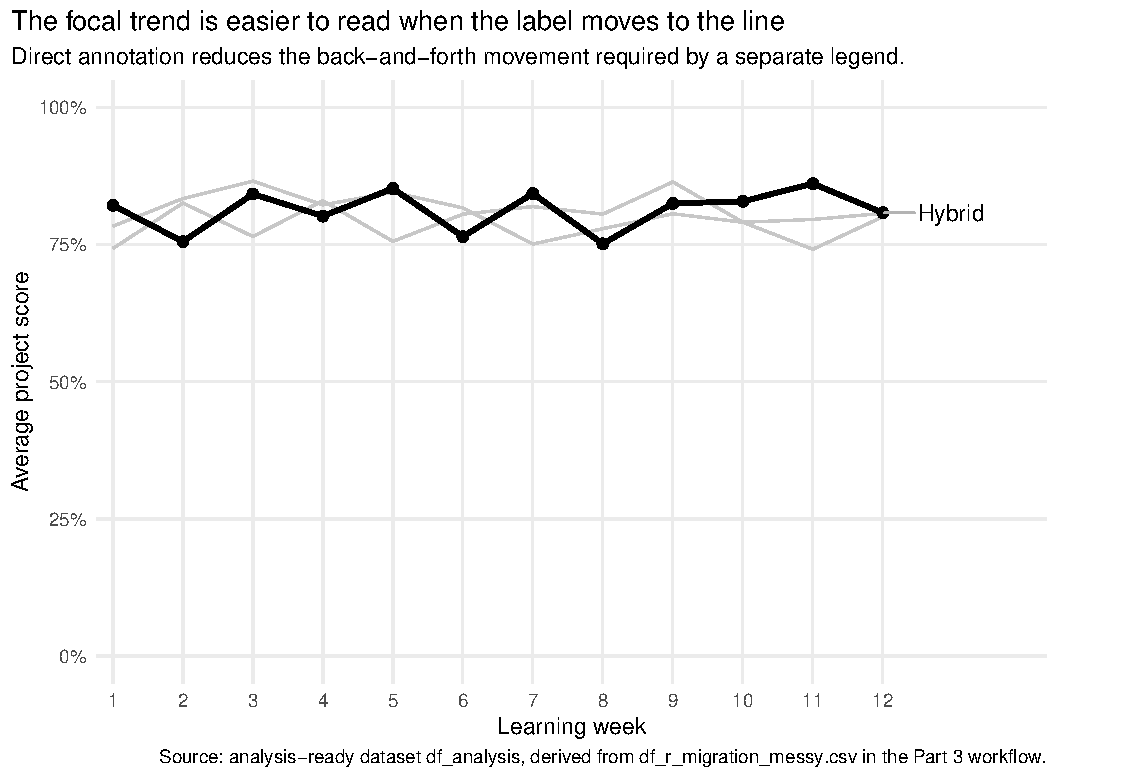
\includegraphics[width=0.9\linewidth,height=\textheight,keepaspectratio,alt={A line chart of average project score across weeks. One highlighted learning mode is labelled directly near the end of its line.}]{chapters/18-communication-from-plots-to-story_files/figure-pdf/fig-18-4-direct-annotation-1.pdf}

}

\caption{\label{fig-18-4-direct-annotation}Direct Annotation Can Replace
a Detached Legend When the Plot Has a Clear Focal Pattern.}

\end{figure}%

The code in Listing~\ref{lst-fig-18-4-direct-annotation} produces
Figure~\ref{fig-18-4-direct-annotation}.

A legend says, ``Decode this colour over there, then come back to the
data.''

A direct label says, ``This line is this group.''

That small move can make a plot feel more humane.

\section{Categorical Narrative
Ordering}\label{categorical-narrative-ordering}

Default category order is rarely the best story order.

R may order character categories alphabetically. Alphabetical order is
sometimes useful, but it is often accidental. If the question is about
which group has the highest average score, the categories should be
ordered by average score. If the question is about frequency, they
should be ordered by count. If the question follows a process, the
categories should follow that process.

The \texttt{forcats} package gives Leo practical tools for this work.

\begin{codelisting}

\caption{\label{lst-fig-18-5-factor-ordering}Code for Reordering
Categories by Value}

\centering{

\begin{Shaded}
\begin{Highlighting}[]
\NormalTok{mode\_summary }\OtherTok{\textless{}{-}}\NormalTok{ df\_story }\SpecialCharTok{\%\textgreater{}\%}
  \FunctionTok{filter}\NormalTok{(}\SpecialCharTok{!}\FunctionTok{is.na}\NormalTok{(preferred\_learning\_mode)) }\SpecialCharTok{\%\textgreater{}\%}
  \FunctionTok{group\_by}\NormalTok{(preferred\_learning\_mode) }\SpecialCharTok{\%\textgreater{}\%}
  \FunctionTok{summarise}\NormalTok{(}
    \AttributeTok{mean\_project =} \FunctionTok{mean}\NormalTok{(project\_score, }\AttributeTok{na.rm =} \ConstantTok{TRUE}\NormalTok{),}
    \AttributeTok{learners =} \FunctionTok{n}\NormalTok{(),}
    \AttributeTok{.groups =} \StringTok{"drop"}
\NormalTok{  ) }\SpecialCharTok{\%\textgreater{}\%}
  \FunctionTok{filter}\NormalTok{(learners }\SpecialCharTok{\textgreater{}=} \DecValTok{5}\NormalTok{) }\SpecialCharTok{\%\textgreater{}\%}
  \FunctionTok{mutate}\NormalTok{(}
    \AttributeTok{preferred\_learning\_mode =}\NormalTok{ forcats}\SpecialCharTok{::}\FunctionTok{fct\_reorder}\NormalTok{(}
\NormalTok{      preferred\_learning\_mode,}
\NormalTok{      mean\_project}
\NormalTok{    )}
\NormalTok{  )}

\FunctionTok{ggplot}\NormalTok{(mode\_summary, }\FunctionTok{aes}\NormalTok{(}\AttributeTok{x =}\NormalTok{ preferred\_learning\_mode, }\AttributeTok{y =}\NormalTok{ mean\_project)) }\SpecialCharTok{+}
  \FunctionTok{geom\_col}\NormalTok{(}\AttributeTok{fill =} \StringTok{"grey45"}\NormalTok{, }\AttributeTok{width =} \FloatTok{0.68}\NormalTok{) }\SpecialCharTok{+}
  \FunctionTok{coord\_flip}\NormalTok{() }\SpecialCharTok{+}
  \FunctionTok{scale\_y\_continuous}\NormalTok{(}\AttributeTok{limits =} \FunctionTok{c}\NormalTok{(}\DecValTok{0}\NormalTok{, }\DecValTok{100}\NormalTok{), }\AttributeTok{labels =}\NormalTok{ scales}\SpecialCharTok{::}\FunctionTok{label\_number}\NormalTok{(}\AttributeTok{suffix =} \StringTok{"\%"}\NormalTok{)) }\SpecialCharTok{+}
  \FunctionTok{labs}\NormalTok{(}
    \AttributeTok{title =} \StringTok{"Ordering categories by value turns a list into a comparison"}\NormalTok{,}
    \AttributeTok{subtitle =} \StringTok{"Preferred learning modes are arranged by average project score."}\NormalTok{,}
    \AttributeTok{x =} \ConstantTok{NULL}\NormalTok{,}
    \AttributeTok{y =} \StringTok{"Average project score"}\NormalTok{,}
    \AttributeTok{caption =}\NormalTok{ chapter18\_caption\_source}
\NormalTok{  ) }\SpecialCharTok{+}
  \FunctionTok{theme\_minimal}\NormalTok{(}\AttributeTok{base\_size =} \DecValTok{11}\NormalTok{) }\SpecialCharTok{+}
  \FunctionTok{theme}\NormalTok{(}
    \AttributeTok{panel.grid.major.y =} \FunctionTok{element\_blank}\NormalTok{(),}
    \AttributeTok{panel.grid.minor =} \FunctionTok{element\_blank}\NormalTok{(),}
    \AttributeTok{plot.title.position =} \StringTok{"plot"}\NormalTok{,}
    \AttributeTok{plot.caption.position =} \StringTok{"plot"}
\NormalTok{  )}
\end{Highlighting}
\end{Shaded}

}

\end{codelisting}%

\begin{figure}[H]

\centering{

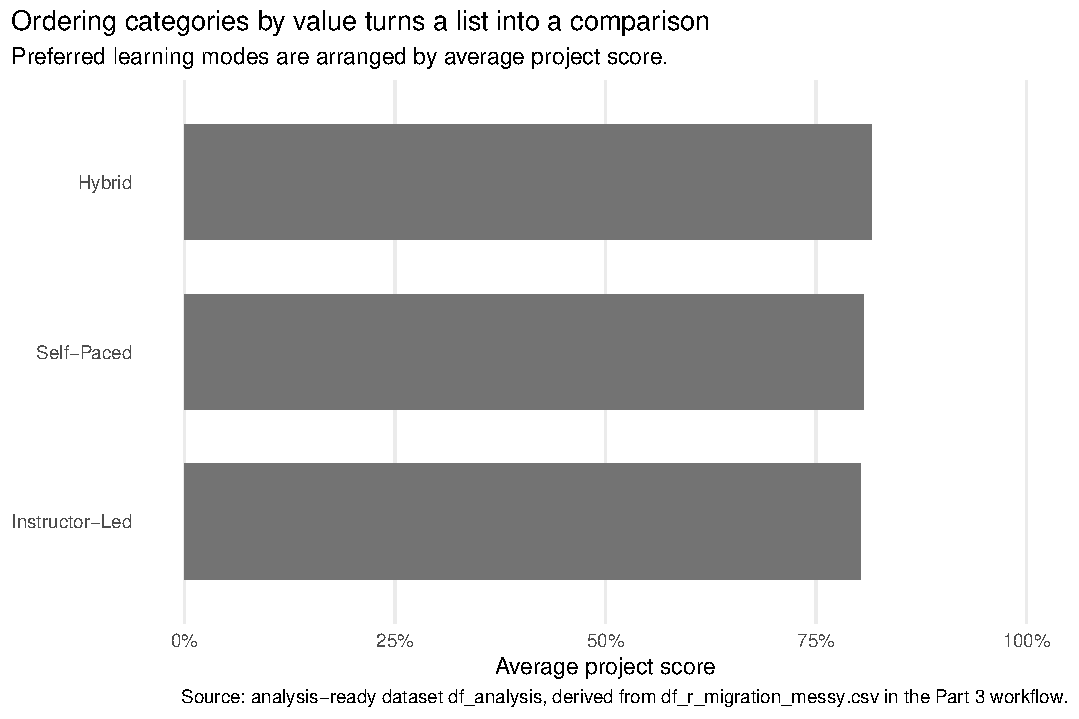
\includegraphics[width=0.9\linewidth,height=\textheight,keepaspectratio,alt={A horizontal bar chart showing average project score by preferred learning mode, ordered from lower to higher average score.}]{chapters/18-communication-from-plots-to-story_files/figure-pdf/fig-18-5-factor-ordering-1.pdf}

}

\caption{\label{fig-18-5-factor-ordering}Reordering Categories by Value
Creates a Clearer Comparison Than Default Ordering.}

\end{figure}%

The code in Listing~\ref{lst-fig-18-5-factor-ordering} produces
Figure~\ref{fig-18-5-factor-ordering}.

Ordering is not a minor detail. It changes how quickly a reader
understands the pattern.

Common ordering choices include:

\begin{codelisting}

\caption{\label{lst-chapter18-forcats-patterns}Code for Common forcats
Ordering Patterns}

\centering{

\begin{Shaded}
\begin{Highlighting}[]
\CommentTok{\# Order by a numeric summary:}
\NormalTok{df\_summary }\SpecialCharTok{\%\textgreater{}\%}
  \FunctionTok{mutate}\NormalTok{(}\AttributeTok{group =}\NormalTok{ forcats}\SpecialCharTok{::}\FunctionTok{fct\_reorder}\NormalTok{(group, average\_score))}

\CommentTok{\# Order by frequency:}
\NormalTok{df\_analysis }\SpecialCharTok{\%\textgreater{}\%}
  \FunctionTok{mutate}\NormalTok{(}\AttributeTok{background =}\NormalTok{ forcats}\SpecialCharTok{::}\FunctionTok{fct\_infreq}\NormalTok{(background))}

\CommentTok{\# Reverse an order:}
\NormalTok{df\_summary }\SpecialCharTok{\%\textgreater{}\%}
  \FunctionTok{mutate}\NormalTok{(}\AttributeTok{group =}\NormalTok{ forcats}\SpecialCharTok{::}\FunctionTok{fct\_rev}\NormalTok{(group))}

\CommentTok{\# Move a category to the front:}
\NormalTok{df\_summary }\SpecialCharTok{\%\textgreater{}\%}
  \FunctionTok{mutate}\NormalTok{(}\AttributeTok{group =}\NormalTok{ forcats}\SpecialCharTok{::}\FunctionTok{fct\_relevel}\NormalTok{(group, }\StringTok{"Completed"}\NormalTok{))}
\end{Highlighting}
\end{Shaded}

}

\end{codelisting}%

The optional code in Listing~\ref{lst-chapter18-forcats-patterns} shows
common \texttt{forcats} ordering patterns Leo can adapt.

Leo should choose the order that matches the reader's task. A chart
about ranking needs value order. A chart about a process needs process
order. A chart about a story may need the order in which the argument
unfolds.

\section{Multi-Plot Compositions}\label{multi-plot-compositions}

Sometimes one plot is not enough. But more plots do not automatically
create a better story.

A multi-plot composition should have a reason. It may show:

\begin{itemize}
\tightlist
\item
  context first, then detail;
\item
  group comparison, then trend;
\item
  trend first, then explanation;
\item
  before and after;
\item
  problem, evidence, and implication.
\end{itemize}

The \texttt{patchwork} package lets Leo combine ggplot objects using a
syntax that feels natural once he already understands ggplot2. The next
figure creates a small visual sequence: who the learners are, how
project scores change across weeks, and how study time relates to
project score.

\begin{codelisting}

\caption{\label{lst-fig-18-6-multi-plot-composition}Code for a
Three-Part Visual Sequence}

\centering{

\begin{Shaded}
\begin{Highlighting}[]
\NormalTok{background\_count\_plot }\OtherTok{\textless{}{-}}\NormalTok{ df\_story }\SpecialCharTok{\%\textgreater{}\%}
  \FunctionTok{filter}\NormalTok{(}\SpecialCharTok{!}\FunctionTok{is.na}\NormalTok{(background)) }\SpecialCharTok{\%\textgreater{}\%}
  \FunctionTok{count}\NormalTok{(background, }\AttributeTok{sort =} \ConstantTok{TRUE}\NormalTok{) }\SpecialCharTok{\%\textgreater{}\%}
  \FunctionTok{mutate}\NormalTok{(}\AttributeTok{background =}\NormalTok{ forcats}\SpecialCharTok{::}\FunctionTok{fct\_reorder}\NormalTok{(background, n)) }\SpecialCharTok{\%\textgreater{}\%}
  \FunctionTok{ggplot}\NormalTok{(}\FunctionTok{aes}\NormalTok{(}\AttributeTok{x =}\NormalTok{ background, }\AttributeTok{y =}\NormalTok{ n)) }\SpecialCharTok{+}
  \FunctionTok{geom\_col}\NormalTok{(}\AttributeTok{fill =} \StringTok{"grey55"}\NormalTok{, }\AttributeTok{width =} \FloatTok{0.68}\NormalTok{) }\SpecialCharTok{+}
  \FunctionTok{coord\_flip}\NormalTok{() }\SpecialCharTok{+}
  \FunctionTok{labs}\NormalTok{(}
    \AttributeTok{title =} \StringTok{"Who is in the data?"}\NormalTok{,}
    \AttributeTok{x =} \ConstantTok{NULL}\NormalTok{,}
    \AttributeTok{y =} \StringTok{"Learners"}
\NormalTok{  ) }\SpecialCharTok{+}
  \FunctionTok{theme\_minimal}\NormalTok{(}\AttributeTok{base\_size =} \DecValTok{10}\NormalTok{) }\SpecialCharTok{+}
  \FunctionTok{theme}\NormalTok{(}
    \AttributeTok{panel.grid.major.y =} \FunctionTok{element\_blank}\NormalTok{(),}
    \AttributeTok{panel.grid.minor =} \FunctionTok{element\_blank}\NormalTok{()}
\NormalTok{  )}

\NormalTok{weekly\_score\_plot }\OtherTok{\textless{}{-}}\NormalTok{ df\_story }\SpecialCharTok{\%\textgreater{}\%}
  \FunctionTok{group\_by}\NormalTok{(week) }\SpecialCharTok{\%\textgreater{}\%}
  \FunctionTok{summarise}\NormalTok{(}\AttributeTok{mean\_project =} \FunctionTok{mean}\NormalTok{(project\_score, }\AttributeTok{na.rm =} \ConstantTok{TRUE}\NormalTok{), }\AttributeTok{.groups =} \StringTok{"drop"}\NormalTok{) }\SpecialCharTok{\%\textgreater{}\%}
  \FunctionTok{ggplot}\NormalTok{(}\FunctionTok{aes}\NormalTok{(}\AttributeTok{x =}\NormalTok{ week, }\AttributeTok{y =}\NormalTok{ mean\_project)) }\SpecialCharTok{+}
  \FunctionTok{geom\_line}\NormalTok{(}\AttributeTok{linewidth =} \FloatTok{0.9}\NormalTok{, }\AttributeTok{colour =} \StringTok{"black"}\NormalTok{) }\SpecialCharTok{+}
  \FunctionTok{geom\_point}\NormalTok{(}\AttributeTok{size =} \FloatTok{1.9}\NormalTok{, }\AttributeTok{colour =} \StringTok{"black"}\NormalTok{) }\SpecialCharTok{+}
  \FunctionTok{scale\_x\_continuous}\NormalTok{(}\AttributeTok{breaks =} \FunctionTok{sort}\NormalTok{(}\FunctionTok{unique}\NormalTok{(df\_story}\SpecialCharTok{$}\NormalTok{week))) }\SpecialCharTok{+}
  \FunctionTok{scale\_y\_continuous}\NormalTok{(}\AttributeTok{limits =} \FunctionTok{c}\NormalTok{(}\DecValTok{0}\NormalTok{, }\DecValTok{100}\NormalTok{), }\AttributeTok{labels =}\NormalTok{ scales}\SpecialCharTok{::}\FunctionTok{label\_number}\NormalTok{(}\AttributeTok{suffix =} \StringTok{"\%"}\NormalTok{)) }\SpecialCharTok{+}
  \FunctionTok{labs}\NormalTok{(}
    \AttributeTok{title =} \StringTok{"What changes over time?"}\NormalTok{,}
    \AttributeTok{x =} \StringTok{"Learning week"}\NormalTok{,}
    \AttributeTok{y =} \StringTok{"Average score"}
\NormalTok{  ) }\SpecialCharTok{+}
  \FunctionTok{theme\_minimal}\NormalTok{(}\AttributeTok{base\_size =} \DecValTok{10}\NormalTok{) }\SpecialCharTok{+}
  \FunctionTok{theme}\NormalTok{(}\AttributeTok{panel.grid.minor =} \FunctionTok{element\_blank}\NormalTok{())}

\NormalTok{study\_score\_plot }\OtherTok{\textless{}{-}} \FunctionTok{ggplot}\NormalTok{(df\_story, }\FunctionTok{aes}\NormalTok{(}\AttributeTok{x =}\NormalTok{ study\_hours, }\AttributeTok{y =}\NormalTok{ project\_score)) }\SpecialCharTok{+}
  \FunctionTok{geom\_point}\NormalTok{(}\AttributeTok{alpha =} \FloatTok{0.25}\NormalTok{, }\AttributeTok{colour =} \StringTok{"grey40"}\NormalTok{) }\SpecialCharTok{+}
  \FunctionTok{geom\_smooth}\NormalTok{(}\AttributeTok{method =} \StringTok{"lm"}\NormalTok{, }\AttributeTok{se =} \ConstantTok{FALSE}\NormalTok{, }\AttributeTok{colour =} \StringTok{"black"}\NormalTok{, }\AttributeTok{linewidth =} \FloatTok{0.8}\NormalTok{) }\SpecialCharTok{+}
  \FunctionTok{scale\_y\_continuous}\NormalTok{(}\AttributeTok{limits =} \FunctionTok{c}\NormalTok{(}\DecValTok{0}\NormalTok{, }\DecValTok{100}\NormalTok{), }\AttributeTok{labels =}\NormalTok{ scales}\SpecialCharTok{::}\FunctionTok{label\_number}\NormalTok{(}\AttributeTok{suffix =} \StringTok{"\%"}\NormalTok{)) }\SpecialCharTok{+}
  \FunctionTok{labs}\NormalTok{(}
    \AttributeTok{title =} \StringTok{"What relationship needs attention?"}\NormalTok{,}
    \AttributeTok{x =} \StringTok{"Weekly study hours"}\NormalTok{,}
    \AttributeTok{y =} \StringTok{"Project score"}
\NormalTok{  ) }\SpecialCharTok{+}
  \FunctionTok{theme\_minimal}\NormalTok{(}\AttributeTok{base\_size =} \DecValTok{10}\NormalTok{) }\SpecialCharTok{+}
  \FunctionTok{theme}\NormalTok{(}\AttributeTok{panel.grid.minor =} \FunctionTok{element\_blank}\NormalTok{())}

\ControlFlowTok{if}\NormalTok{ (}\FunctionTok{chapter18\_has\_pkg}\NormalTok{(}\StringTok{"patchwork"}\NormalTok{)) \{}
\NormalTok{  (background\_count\_plot }\SpecialCharTok{|}\NormalTok{ weekly\_score\_plot) }\SpecialCharTok{/}\NormalTok{ study\_score\_plot }\SpecialCharTok{+}
\NormalTok{    patchwork}\SpecialCharTok{::}\FunctionTok{plot\_annotation}\NormalTok{(}
      \AttributeTok{title =} \StringTok{"A visual story can move from context to pattern to interpretation"}\NormalTok{,}
      \AttributeTok{subtitle =} \StringTok{"The sequence matters because it controls how the reader enters the evidence."}\NormalTok{,}
      \AttributeTok{caption =}\NormalTok{ chapter18\_caption\_source,}
      \AttributeTok{tag\_levels =} \StringTok{"A"}
\NormalTok{    )}
\NormalTok{\} }\ControlFlowTok{else}\NormalTok{ \{}
\NormalTok{  study\_score\_plot }\SpecialCharTok{+}
    \FunctionTok{labs}\NormalTok{(}
      \AttributeTok{title =} \StringTok{"A visual story can move from context to pattern to interpretation"}\NormalTok{,}
      \AttributeTok{subtitle =} \StringTok{"Install patchwork to combine this plot with the context and trend panels."}\NormalTok{,}
      \AttributeTok{caption =}\NormalTok{ chapter18\_caption\_source}
\NormalTok{    )}
\NormalTok{\}}
\end{Highlighting}
\end{Shaded}

}

\end{codelisting}%

\begin{figure}[H]

\centering{

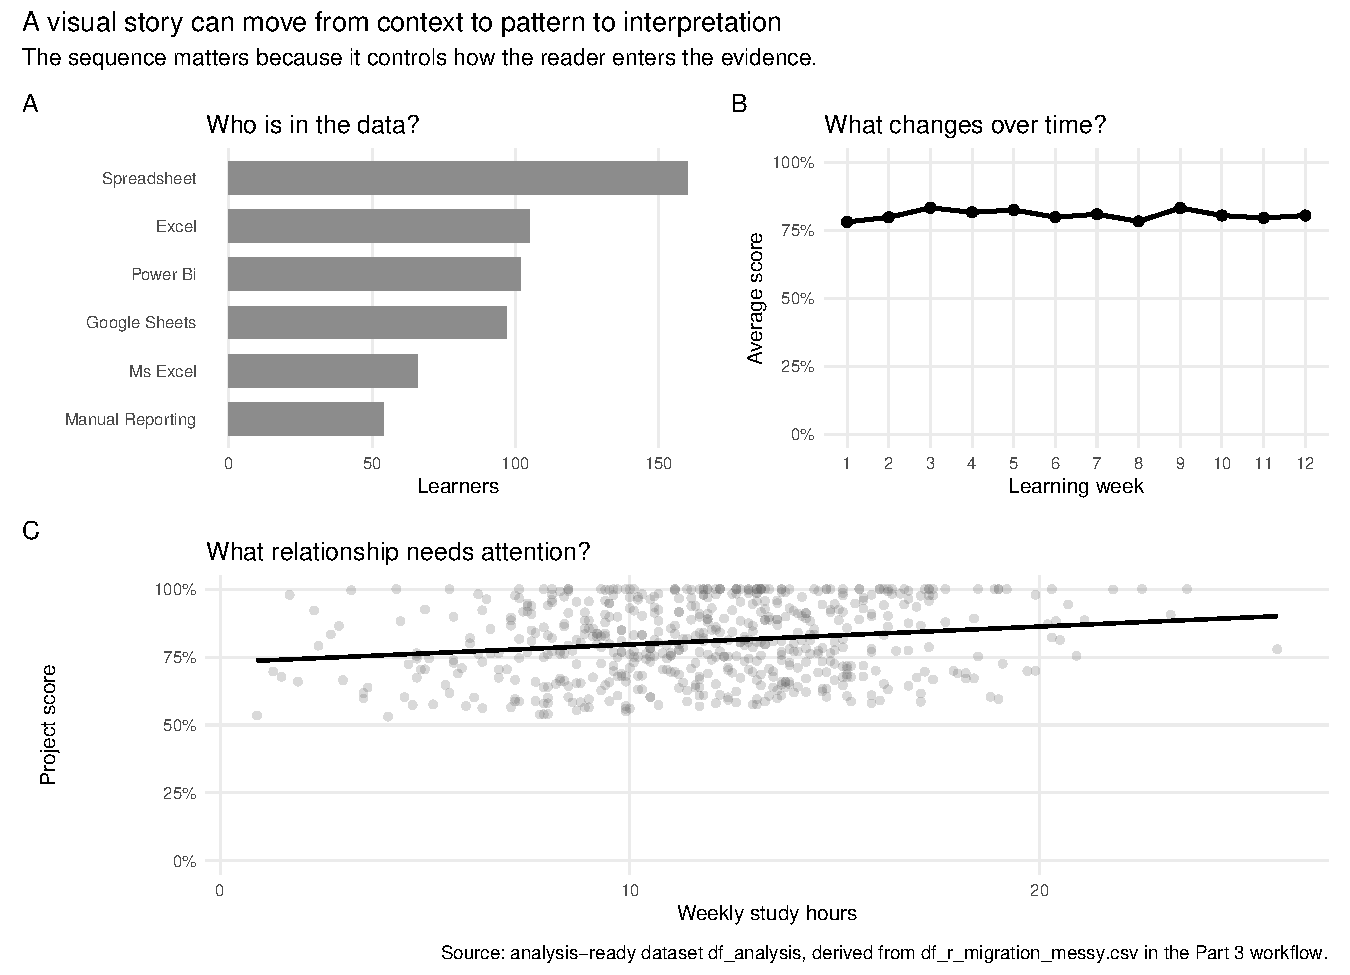
\includegraphics[width=0.9\linewidth,height=\textheight,keepaspectratio,alt={A composite figure with three plots: learner background counts, weekly average project score, and study hours against project score.}]{chapters/18-communication-from-plots-to-story_files/figure-pdf/fig-18-6-multi-plot-composition-1.pdf}

}

\caption{\label{fig-18-6-multi-plot-composition}A Three-Part Visual
Sequence Can Guide the Reader from Context to Trend to Relationship.}

\end{figure}%

The code in Listing~\ref{lst-fig-18-6-multi-plot-composition} produces
Figure~\ref{fig-18-6-multi-plot-composition}.

A multi-panel figure should not feel like a storage container for every
plot Leo made. It should feel like a guided path.

\begin{tcolorbox}[enhanced jigsaw, arc=.35mm, bottomrule=.15mm, breakable, colback=white, colframe=quarto-callout-tip-color-frame, left=2mm, leftrule=.75mm, opacityback=0, rightrule=.15mm, toprule=.15mm]
\begin{minipage}[t]{5.5mm}
\textcolor{quarto-callout-tip-color}{\faLightbulb}
\end{minipage}%
\begin{minipage}[t]{\textwidth - 5.5mm}

\vspace{-3mm}\textbf{Ask before combining plots}\vspace{3mm}

Before using \texttt{patchwork}, Leo should ask:

\textbf{Do these plots answer one larger question together?}

If the answer is no, they may belong in separate sections rather than
one composite figure.

\end{minipage}%
\end{tcolorbox}

\section{Clarity and Control Problems in R
Visualization}\label{clarity-and-control-problems-in-r-visualization}

The following table is intentionally direct. It lists common clarity and
control problems R users face in data visualization and practical ways
out.

\begin{Shaded}
\begin{Highlighting}[]
\NormalTok{tibble}\SpecialCharTok{::}\FunctionTok{tribble}\NormalTok{(}
  \SpecialCharTok{\textasciitilde{}}\StringTok{\textasciigrave{}}\AttributeTok{Clarity or Control Problem}\StringTok{\textasciigrave{}}\NormalTok{, }\SpecialCharTok{\textasciitilde{}}\StringTok{\textasciigrave{}}\AttributeTok{Way Out}\StringTok{\textasciigrave{}}\NormalTok{,}
  \StringTok{"Cluttered plot"}\NormalTok{, }\StringTok{"Remove non{-}essential layers, reduce gridlines, simplify geoms."}\NormalTok{,}
  \StringTok{"Weak visual hierarchy"}\NormalTok{, }\StringTok{"Make title, focal data, labels, and caption visually distinct."}\NormalTok{,}
  \StringTok{"Detached legend slows reading"}\NormalTok{, }\StringTok{"Use direct labels or simplify legend placement."}\NormalTok{,}
  \StringTok{"Confusing category order"}\NormalTok{, }\StringTok{"Reorder factors with \textasciigrave{}forcats::fct\_reorder()\textasciigrave{} or \textasciigrave{}forcats::fct\_infreq()\textasciigrave{}."}\NormalTok{,}
  \StringTok{"Unreadable labels"}\NormalTok{, }\StringTok{"Shorten labels, flip coordinates, increase text size, or use \textasciigrave{}ggrepel\textasciigrave{}."}\NormalTok{,}
  \StringTok{"Inaccessible colour choices"}\NormalTok{, }\StringTok{"Use colour{-}blind aware palettes and avoid colour{-}only meaning."}\NormalTok{,}
  \StringTok{"Inconsistent fonts"}\NormalTok{, }\StringTok{"Set a deliberate base font and verify system font availability."}\NormalTok{,}
  \StringTok{"Overplotting"}\NormalTok{, }\StringTok{"Use transparency, jitter, binning, summaries, or sampling."}\NormalTok{,}
  \StringTok{"Poorly cropped exports"}\NormalTok{, }\StringTok{"Set width, height, units, and margins before saving."}\NormalTok{,}
  \StringTok{"Low{-}resolution images"}\NormalTok{, }\StringTok{"Use higher DPI for raster output or export vector formats."}\NormalTok{,}
  \StringTok{"Weak titles"}\NormalTok{, }\StringTok{"Write message{-}led titles that guide interpretation."}\NormalTok{,}
  \StringTok{"Unhelpful captions"}\NormalTok{, }\StringTok{"State source, scope, filters, and necessary limits."}\NormalTok{,}
  \StringTok{"Misleading scales"}\NormalTok{, }\StringTok{"Check axis limits, transformations, breaks, and removed data."}\NormalTok{,}
  \StringTok{"Different{-}looking plots across devices"}\NormalTok{, }\StringTok{"Use explicit theme settings, fonts, sizes, and export devices."}\NormalTok{,}
  \StringTok{"Too many highlighted groups"}\NormalTok{, }\StringTok{"Highlight fewer groups or split the story into separate plots."}\NormalTok{,}
  \StringTok{"Annotation covers the data"}\NormalTok{, }\StringTok{"Move labels, use \textasciigrave{}ggrepel\textasciigrave{}, or annotate outside the panel."}\NormalTok{,}
  \StringTok{"Colour used as decoration"}\NormalTok{, }\StringTok{"Assign colour only when it carries meaning."}\NormalTok{,}
  \StringTok{"Multi{-}panel plot feels crowded"}\NormalTok{, }\StringTok{"Reduce panels, align axes, or split into a sequence."}\NormalTok{,}
  \StringTok{"Plot does not answer the question"}\NormalTok{, }\StringTok{"Rewrite the visual question before editing the design."}\NormalTok{,}
  \StringTok{"Export does not fit slides or reports"}\NormalTok{, }\StringTok{"Use exact aspect ratios and destination{-}specific \textasciigrave{}ggsave()\textasciigrave{} settings."}
\NormalTok{) }\SpecialCharTok{\%\textgreater{}\%}
\NormalTok{  knitr}\SpecialCharTok{::}\FunctionTok{kable}\NormalTok{()}
\end{Highlighting}
\end{Shaded}

{

\begin{longtable}[]{@{}
  >{\raggedright\arraybackslash}p{(\linewidth - 2\tabcolsep) * \real{0.3451}}
  >{\raggedright\arraybackslash}p{(\linewidth - 2\tabcolsep) * \real{0.6549}}@{}}

\caption{\label{tbl-18-4-clarity-control-problems}Clarity and Control
Problems in R Visualization and Practical Ways Out.}

\tabularnewline

\toprule\noalign{}
\begin{minipage}[b]{\linewidth}\raggedright
Clarity or Control Problem
\end{minipage} & \begin{minipage}[b]{\linewidth}\raggedright
Way Out
\end{minipage} \\
\midrule\noalign{}
\endhead
\bottomrule\noalign{}
\endlastfoot
Cluttered plot & Remove non-essential layers, reduce gridlines, simplify
geoms. \\
Weak visual hierarchy & Make title, focal data, labels, and caption
visually distinct. \\
Detached legend slows reading & Use direct labels or simplify legend
placement. \\
Confusing category order & Reorder factors with
\texttt{forcats::fct\_reorder()} or \texttt{forcats::fct\_infreq()}. \\
Unreadable labels & Shorten labels, flip coordinates, increase text
size, or use \texttt{ggrepel}. \\
Inaccessible colour choices & Use colour-blind aware palettes and avoid
colour-only meaning. \\
Inconsistent fonts & Set a deliberate base font and verify system font
availability. \\
Overplotting & Use transparency, jitter, binning, summaries, or
sampling. \\
Poorly cropped exports & Set width, height, units, and margins before
saving. \\
Low-resolution images & Use higher DPI for raster output or export
vector formats. \\
Weak titles & Write message-led titles that guide interpretation. \\
Unhelpful captions & State source, scope, filters, and necessary
limits. \\
Misleading scales & Check axis limits, transformations, breaks, and
removed data. \\
Different-looking plots across devices & Use explicit theme settings,
fonts, sizes, and export devices. \\
Too many highlighted groups & Highlight fewer groups or split the story
into separate plots. \\
Annotation covers the data & Move labels, use \texttt{ggrepel}, or
annotate outside the panel. \\
Colour used as decoration & Assign colour only when it carries
meaning. \\
Multi-panel plot feels crowded & Reduce panels, align axes, or split
into a sequence. \\
Plot does not answer the question & Rewrite the visual question before
editing the design. \\
Export does not fit slides or reports & Use exact aspect ratios and
destination-specific \texttt{ggsave()} settings. \\

\end{longtable}

}

Table~\ref{tbl-18-4-clarity-control-problems} is a repair map. When a
plot feels wrong, Leo should not guess randomly. He should name the
failure, then choose a targeted fix.

\section{Accessible and Inclusive
Design}\label{accessible-and-inclusive-design}

Accessibility is not an optional finishing touch. It is part of
responsible communication.

A plot is accessible when more people can read it accurately. That
includes people with colour-vision differences, low vision,
screen-reader users, readers viewing a plot on a small screen, readers
printing in grayscale, and readers who are not familiar with the
analyst's context.

Accessible design includes four habits.

First, do not rely on colour alone. If colour distinguishes groups,
consider adding direct labels, line types, shapes, or facets.

Second, use sufficient contrast. Pale text on a pale background may look
elegant on a designer's monitor and become unreadable in a classroom
projector, printed handout, or compressed PDF.

Third, keep text meaningful. A title like ``Figure 3'' is not accessible
guidance. A title that states the main comparison helps everyone.

Fourth, write alt text. Alt text should describe the chart type, the
variables, the main pattern, and any important caution.

\begin{Shaded}
\begin{Highlighting}[]
\NormalTok{tibble}\SpecialCharTok{::}\FunctionTok{tribble}\NormalTok{(}
  \SpecialCharTok{\textasciitilde{}}\StringTok{\textasciigrave{}}\AttributeTok{Alt Text Element}\StringTok{\textasciigrave{}}\NormalTok{, }\SpecialCharTok{\textasciitilde{}}\StringTok{\textasciigrave{}}\AttributeTok{Question to Answer}\StringTok{\textasciigrave{}}\NormalTok{, }\SpecialCharTok{\textasciitilde{}}\StringTok{\textasciigrave{}}\AttributeTok{Example}\StringTok{\textasciigrave{}}\NormalTok{,}
  \StringTok{"Chart type"}\NormalTok{, }\StringTok{"What kind of visual is this?"}\NormalTok{, }\StringTok{"A line chart..."}\NormalTok{,}
  \StringTok{"Variables"}\NormalTok{, }\StringTok{"What is being compared or measured?"}\NormalTok{, }\StringTok{"...showing average project score by learning week..."}\NormalTok{,}
  \StringTok{"Main pattern"}\NormalTok{, }\StringTok{"What should the reader notice?"}\NormalTok{, }\StringTok{"...with scores generally increasing across the weeks..."}\NormalTok{,}
  \StringTok{"Focal detail"}\NormalTok{, }\StringTok{"Is any group highlighted?"}\NormalTok{, }\StringTok{"...and the project{-}based learning mode highlighted as the strongest final trend."}\NormalTok{,}
  \StringTok{"Limit"}\NormalTok{, }\StringTok{"What should not be overclaimed?"}\NormalTok{, }\StringTok{"The chart shows association over time, not proof that the learning mode caused the score increase."}
\NormalTok{) }\SpecialCharTok{\%\textgreater{}\%}
\NormalTok{  knitr}\SpecialCharTok{::}\FunctionTok{kable}\NormalTok{()}
\end{Highlighting}
\end{Shaded}

{

\begin{longtable}[]{@{}
  >{\raggedright\arraybackslash}p{(\linewidth - 4\tabcolsep) * \real{0.1118}}
  >{\raggedright\arraybackslash}p{(\linewidth - 4\tabcolsep) * \real{0.2368}}
  >{\raggedright\arraybackslash}p{(\linewidth - 4\tabcolsep) * \real{0.6513}}@{}}

\caption{\label{tbl-18-5-alt-text-pattern}A Practical Pattern for
Writing alt Text for Data Visualizations.}

\tabularnewline

\toprule\noalign{}
\begin{minipage}[b]{\linewidth}\raggedright
Alt Text Element
\end{minipage} & \begin{minipage}[b]{\linewidth}\raggedright
Question to Answer
\end{minipage} & \begin{minipage}[b]{\linewidth}\raggedright
Example
\end{minipage} \\
\midrule\noalign{}
\endhead
\bottomrule\noalign{}
\endlastfoot
Chart type & What kind of visual is this? & A line chart\ldots{} \\
Variables & What is being compared or measured? & \ldots showing average
project score by learning week\ldots{} \\
Main pattern & What should the reader notice? & \ldots with scores
generally increasing across the weeks\ldots{} \\
Focal detail & Is any group highlighted? & \ldots and the project-based
learning mode highlighted as the strongest final trend. \\
Limit & What should not be overclaimed? & The chart shows association
over time, not proof that the learning mode caused the score
increase. \\

\end{longtable}

}

Table~\ref{tbl-18-5-alt-text-pattern} gives Leo a practical pattern for
writing alt text.

Good alt text is not a decorative description. It is a compressed
explanation of the visual evidence.

\begin{tcolorbox}[enhanced jigsaw, arc=.35mm, bottomrule=.15mm, breakable, colback=white, colframe=quarto-callout-note-color-frame, left=2mm, leftrule=.75mm, opacityback=0, rightrule=.15mm, toprule=.15mm]
\begin{minipage}[t]{5.5mm}
\textcolor{quarto-callout-note-color}{\faInfo}
\end{minipage}%
\begin{minipage}[t]{\textwidth - 5.5mm}

\vspace{-3mm}\textbf{A simple alt-text formula}\vspace{3mm}

\textbf{Chart type + variables + main pattern + highlighted detail +
limit.}

Example: \emph{A scatter plot showing weekly study hours and project
score. Points trend upward, suggesting that learners who report more
study hours tend to have higher project scores. The plot shows
association, not causation.}

\end{minipage}%
\end{tcolorbox}

\section{Responsible Claims: Description, Interpretation, and
Claim}\label{responsible-claims-description-interpretation-and-claim}

A visual story can become dangerous when Leo lets the plot say more than
the evidence supports.

He should separate three layers:

\begin{Shaded}
\begin{Highlighting}[]
\NormalTok{tibble}\SpecialCharTok{::}\FunctionTok{tribble}\NormalTok{(}
  \SpecialCharTok{\textasciitilde{}}\StringTok{\textasciigrave{}}\AttributeTok{Layer}\StringTok{\textasciigrave{}}\NormalTok{, }\SpecialCharTok{\textasciitilde{}}\StringTok{\textasciigrave{}}\AttributeTok{What It Does}\StringTok{\textasciigrave{}}\NormalTok{, }\SpecialCharTok{\textasciitilde{}}\StringTok{\textasciigrave{}}\AttributeTok{Example}\StringTok{\textasciigrave{}}\NormalTok{,}
  \StringTok{"Description"}\NormalTok{, }\StringTok{"States what is visible in the plot."}\NormalTok{, }\StringTok{"Average project scores are higher among learners who report more weekly study hours."}\NormalTok{,}
  \StringTok{"Interpretation"}\NormalTok{, }\StringTok{"Offers a careful reading of what the pattern may mean."}\NormalTok{, }\StringTok{"This may suggest that sustained practice is associated with stronger project performance."}\NormalTok{,}
  \StringTok{"Claim"}\NormalTok{, }\StringTok{"Connects the evidence to an argument or decision."}\NormalTok{, }\StringTok{"The programme should treat structured study time as an important support condition, while testing other explanations before making causal claims."}
\NormalTok{) }\SpecialCharTok{\%\textgreater{}\%}
\NormalTok{  knitr}\SpecialCharTok{::}\FunctionTok{kable}\NormalTok{()}
\end{Highlighting}
\end{Shaded}

{

\begin{longtable}[]{@{}
  >{\raggedright\arraybackslash}p{(\linewidth - 4\tabcolsep) * \real{0.0694}}
  >{\raggedright\arraybackslash}p{(\linewidth - 4\tabcolsep) * \real{0.2546}}
  >{\raggedright\arraybackslash}p{(\linewidth - 4\tabcolsep) * \real{0.6759}}@{}}

\caption{\label{tbl-18-6-description-interpretation-claim}Separating
Description, Interpretation, and Claim in Visual Communication.}

\tabularnewline

\toprule\noalign{}
\begin{minipage}[b]{\linewidth}\raggedright
Layer
\end{minipage} & \begin{minipage}[b]{\linewidth}\raggedright
What It Does
\end{minipage} & \begin{minipage}[b]{\linewidth}\raggedright
Example
\end{minipage} \\
\midrule\noalign{}
\endhead
\bottomrule\noalign{}
\endlastfoot
Description & States what is visible in the plot. & Average project
scores are higher among learners who report more weekly study hours. \\
Interpretation & Offers a careful reading of what the pattern may mean.
& This may suggest that sustained practice is associated with stronger
project performance. \\
Claim & Connects the evidence to an argument or decision. & The
programme should treat structured study time as an important support
condition, while testing other explanations before making causal
claims. \\

\end{longtable}

}

Table~\ref{tbl-18-6-description-interpretation-claim} separates
description, interpretation, and claim.

Description is closest to the plot. Interpretation adds meaning. Claim
adds judgment.

Leo should not jump from description to claim without acknowledging the
bridge. A scatter plot can show association. It cannot, by itself, prove
cause. A bar chart can show a group difference. It cannot, by itself,
prove that the group identity produced the difference.

This is not weakness. It is credibility.

\section{Production-Grade Exporting}\label{production-grade-exporting}

A plot that looks good inside RStudio can fail when exported. It may
appear blurry in a slide deck, too small in a Word document, badly
cropped in a PDF, or inconsistent across computers.

Exporting is part of the visualization workflow, not an afterthought.

The main tool Leo will use is \texttt{ggsave()}. It saves the most
recent plot by default, but a safer practice is to save a named plot
object.

\begin{codelisting}

\caption{\label{lst-chapter18-basic-ggsave}Code for Saving a Named Plot
with ggsave()}

\centering{

\begin{Shaded}
\begin{Highlighting}[]
\NormalTok{final\_plot }\OtherTok{\textless{}{-}} \FunctionTok{ggplot}\NormalTok{(df\_story, }\FunctionTok{aes}\NormalTok{(}\AttributeTok{x =}\NormalTok{ study\_hours, }\AttributeTok{y =}\NormalTok{ project\_score)) }\SpecialCharTok{+}
  \FunctionTok{geom\_point}\NormalTok{(}\AttributeTok{alpha =} \FloatTok{0.3}\NormalTok{) }\SpecialCharTok{+}
  \FunctionTok{geom\_smooth}\NormalTok{(}\AttributeTok{method =} \StringTok{"lm"}\NormalTok{, }\AttributeTok{se =} \ConstantTok{FALSE}\NormalTok{) }\SpecialCharTok{+}
  \FunctionTok{labs}\NormalTok{(}
    \AttributeTok{title =} \StringTok{"Study time and project performance move together"}\NormalTok{,}
    \AttributeTok{x =} \StringTok{"Weekly study hours"}\NormalTok{,}
    \AttributeTok{y =} \StringTok{"Project score"}\NormalTok{,}
    \AttributeTok{caption =}\NormalTok{ chapter18\_caption\_source}
\NormalTok{  ) }\SpecialCharTok{+}
  \FunctionTok{theme\_minimal}\NormalTok{(}\AttributeTok{base\_size =} \DecValTok{11}\NormalTok{)}

\FunctionTok{ggsave}\NormalTok{(}
  \AttributeTok{filename =} \StringTok{"figures/chapter{-}18{-}study{-}score.png"}\NormalTok{,}
  \AttributeTok{plot =}\NormalTok{ final\_plot,}
  \AttributeTok{width =} \DecValTok{7}\NormalTok{,}
  \AttributeTok{height =} \DecValTok{5}\NormalTok{,}
  \AttributeTok{units =} \StringTok{"in"}\NormalTok{,}
  \AttributeTok{dpi =} \DecValTok{300}
\NormalTok{)}
\end{Highlighting}
\end{Shaded}

}

\end{codelisting}%

The code in Listing~\ref{lst-chapter18-basic-ggsave} shows the safer
named-plot export pattern.

For screen use, PNG is often convenient. For print and publication
workflows, PDF or SVG may be better because vector graphics preserve
sharp text and lines when resized.

\begin{codelisting}

\caption{\label{lst-chapter18-vector-export}Code for PDF and SVG Vector
Export}

\centering{

\begin{Shaded}
\begin{Highlighting}[]
\CommentTok{\# PDF vector export:}
\FunctionTok{ggsave}\NormalTok{(}
  \AttributeTok{filename =} \StringTok{"figures/chapter{-}18{-}study{-}score.pdf"}\NormalTok{,}
  \AttributeTok{plot =}\NormalTok{ final\_plot,}
  \AttributeTok{width =} \DecValTok{7}\NormalTok{,}
  \AttributeTok{height =} \DecValTok{5}\NormalTok{,}
  \AttributeTok{units =} \StringTok{"in"}
\NormalTok{)}

\CommentTok{\# SVG vector export:}
\CommentTok{\# This usually requires the svglite package.}
\FunctionTok{ggsave}\NormalTok{(}
  \AttributeTok{filename =} \StringTok{"figures/chapter{-}18{-}study{-}score.svg"}\NormalTok{,}
  \AttributeTok{plot =}\NormalTok{ final\_plot,}
  \AttributeTok{width =} \DecValTok{7}\NormalTok{,}
  \AttributeTok{height =} \DecValTok{5}\NormalTok{,}
  \AttributeTok{units =} \StringTok{"in"}
\NormalTok{)}
\end{Highlighting}
\end{Shaded}

}

\end{codelisting}%

The code in Listing~\ref{lst-chapter18-vector-export} shows PDF and SVG
export patterns.

For slides, Leo should think in aspect ratios. A widescreen slide
usually uses a 16:9 ratio. A common export size is 13.333 by 7.5 inches.

\begin{codelisting}

\caption{\label{lst-chapter18-slide-export}Code for Exporting a Plot at
a 16:9 Slide Ratio}

\centering{

\begin{Shaded}
\begin{Highlighting}[]
\FunctionTok{ggsave}\NormalTok{(}
  \AttributeTok{filename =} \StringTok{"figures/chapter{-}18{-}slide{-}visual.png"}\NormalTok{,}
  \AttributeTok{plot =}\NormalTok{ final\_plot,}
  \AttributeTok{width =} \FloatTok{13.333}\NormalTok{,}
  \AttributeTok{height =} \FloatTok{7.5}\NormalTok{,}
  \AttributeTok{units =} \StringTok{"in"}\NormalTok{,}
  \AttributeTok{dpi =} \DecValTok{300}
\NormalTok{)}
\end{Highlighting}
\end{Shaded}

}

\end{codelisting}%

The code in Listing~\ref{lst-chapter18-slide-export} shows a widescreen
slide export pattern.

Colour profiles require care. A typical R plotting workflow is usually
designed around screen-oriented colour. Professional print workflows may
require CMYK conversion or publisher-specific colour handling. Leo
should not assume that \texttt{ggsave()} alone solves every print
production requirement. When a publisher requests CMYK, he should check
the publisher's figure instructions and, where necessary, export a
high-quality vector or high-resolution raster file for conversion in an
appropriate design or prepress workflow.

\begin{Shaded}
\begin{Highlighting}[]
\NormalTok{tibble}\SpecialCharTok{::}\FunctionTok{tribble}\NormalTok{(}
  \SpecialCharTok{\textasciitilde{}}\StringTok{\textasciigrave{}}\AttributeTok{Destination}\StringTok{\textasciigrave{}}\NormalTok{, }\SpecialCharTok{\textasciitilde{}}\StringTok{\textasciigrave{}}\AttributeTok{Recommended Format}\StringTok{\textasciigrave{}}\NormalTok{, }\SpecialCharTok{\textasciitilde{}}\StringTok{\textasciigrave{}}\AttributeTok{Typical Settings}\StringTok{\textasciigrave{}}\NormalTok{, }\SpecialCharTok{\textasciitilde{}}\StringTok{\textasciigrave{}}\AttributeTok{Main Concern}\StringTok{\textasciigrave{}}\NormalTok{,}
  \StringTok{"Web page"}\NormalTok{, }\StringTok{"PNG or SVG"}\NormalTok{, }\StringTok{"Moderate width; readable text; compressed responsibly"}\NormalTok{, }\StringTok{"Fast loading and screen clarity"}\NormalTok{,}
  \StringTok{"Slide deck"}\NormalTok{, }\StringTok{"PNG"}\NormalTok{, }\StringTok{"16:9 ratio such as 13.333 × 7.5 inches; 150{-}300 DPI"}\NormalTok{, }\StringTok{"Readable from a distance"}\NormalTok{,}
  \StringTok{"Word document"}\NormalTok{, }\StringTok{"PNG or PDF"}\NormalTok{, }\StringTok{"Match document column width; 300 DPI for raster images"}\NormalTok{, }\StringTok{"Avoid blurry resizing"}\NormalTok{,}
  \StringTok{"Academic manuscript"}\NormalTok{, }\StringTok{"PDF, TIFF, PNG, or EPS depending on publisher"}\NormalTok{, }\StringTok{"Follow journal or publisher instructions exactly"}\NormalTok{, }\StringTok{"Submission compliance"}\NormalTok{,}
  \StringTok{"Print layout"}\NormalTok{, }\StringTok{"PDF or high{-}resolution raster"}\NormalTok{, }\StringTok{"Confirm colour, size, and resolution requirements"}\NormalTok{, }\StringTok{"Sharpness and colour reproduction"}\NormalTok{,}
  \StringTok{"Reproducible report"}\NormalTok{, }\StringTok{"Generated inside Quarto"}\NormalTok{, }\StringTok{"Let the document render the figure from source code"}\NormalTok{, }\StringTok{"Keeping code, result, and explanation together"}
\NormalTok{) }\SpecialCharTok{\%\textgreater{}\%}
\NormalTok{  knitr}\SpecialCharTok{::}\FunctionTok{kable}\NormalTok{()}
\end{Highlighting}
\end{Shaded}

{

\begin{longtable}[]{@{}
  >{\raggedright\arraybackslash}p{(\linewidth - 6\tabcolsep) * \real{0.1190}}
  >{\raggedright\arraybackslash}p{(\linewidth - 6\tabcolsep) * \real{0.2738}}
  >{\raggedright\arraybackslash}p{(\linewidth - 6\tabcolsep) * \real{0.3274}}
  >{\raggedright\arraybackslash}p{(\linewidth - 6\tabcolsep) * \real{0.2798}}@{}}

\caption{\label{tbl-18-7-export-decisions}Choosing Export Settings for
Common Visualization Destinations.}

\tabularnewline

\toprule\noalign{}
\begin{minipage}[b]{\linewidth}\raggedright
Destination
\end{minipage} & \begin{minipage}[b]{\linewidth}\raggedright
Recommended Format
\end{minipage} & \begin{minipage}[b]{\linewidth}\raggedright
Typical Settings
\end{minipage} & \begin{minipage}[b]{\linewidth}\raggedright
Main Concern
\end{minipage} \\
\midrule\noalign{}
\endhead
\bottomrule\noalign{}
\endlastfoot
Web page & PNG or SVG & Moderate width; readable text; compressed
responsibly & Fast loading and screen clarity \\
Slide deck & PNG & 16:9 ratio such as 13.333 × 7.5 inches; 150-300 DPI &
Readable from a distance \\
Word document & PNG or PDF & Match document column width; 300 DPI for
raster images & Avoid blurry resizing \\
Academic manuscript & PDF, TIFF, PNG, or EPS depending on publisher &
Follow journal or publisher instructions exactly & Submission
compliance \\
Print layout & PDF or high-resolution raster & Confirm colour, size, and
resolution requirements & Sharpness and colour reproduction \\
Reproducible report & Generated inside Quarto & Let the document render
the figure from source code & Keeping code, result, and explanation
together \\

\end{longtable}

}

Table~\ref{tbl-18-7-export-decisions} summarizes common export decisions
for different destinations.

Exporting is where visual communication meets delivery. A strong plot
should not become weak at the final step.

\section{A Practical Story Workflow}\label{a-practical-story-workflow}

By now, Leo has many tools: grammar of graphics, scales, themes, labels,
annotations, ordering, highlighting, accessibility, and export settings.
The challenge is not knowing that these tools exist. The challenge is
knowing what order to use them in.

A practical workflow looks like this:

\begin{Shaded}
\begin{Highlighting}[]
\NormalTok{tibble}\SpecialCharTok{::}\FunctionTok{tribble}\NormalTok{(}
  \SpecialCharTok{\textasciitilde{}}\StringTok{\textasciigrave{}}\AttributeTok{Step}\StringTok{\textasciigrave{}}\NormalTok{, }\SpecialCharTok{\textasciitilde{}}\StringTok{\textasciigrave{}}\AttributeTok{Question}\StringTok{\textasciigrave{}}\NormalTok{, }\SpecialCharTok{\textasciitilde{}}\StringTok{\textasciigrave{}}\AttributeTok{Action}\StringTok{\textasciigrave{}}\NormalTok{,}
  \StringTok{"1. Name the purpose"}\NormalTok{, }\StringTok{"What should the reader see?"}\NormalTok{, }\StringTok{"Write the one{-}sentence message before polishing."}\NormalTok{,}
  \StringTok{"2. Choose the evidence"}\NormalTok{, }\StringTok{"Which variables and summaries support the message?"}\NormalTok{, }\StringTok{"Select the plot type that matches the analytical question."}\NormalTok{,}
  \StringTok{"3. Create the basic plot"}\NormalTok{, }\StringTok{"Is the evidence visible?"}\NormalTok{, }\StringTok{"Build a simple correct ggplot first."}\NormalTok{,}
  \StringTok{"4. Order the reading path"}\NormalTok{, }\StringTok{"Where should the eye go first?"}\NormalTok{, }\StringTok{"Use title, ordering, contrast, and layout."}\NormalTok{,}
  \StringTok{"5. Reduce noise"}\NormalTok{, }\StringTok{"What distracts from the evidence?"}\NormalTok{, }\StringTok{"Remove clutter, quiet background lines, and simplify legends."}\NormalTok{,}
  \StringTok{"6. Add guidance"}\NormalTok{, }\StringTok{"Where might the reader need help?"}\NormalTok{, }\StringTok{"Use subtitles, direct labels, annotations, and captions."}\NormalTok{,}
  \StringTok{"7. Check responsibility"}\NormalTok{, }\StringTok{"What can the plot support?"}\NormalTok{, }\StringTok{"Separate description, interpretation, and claim."}\NormalTok{,}
  \StringTok{"8. Check accessibility"}\NormalTok{, }\StringTok{"Who might struggle to read this?"}\NormalTok{, }\StringTok{"Review colour, contrast, text, and alt text."}\NormalTok{,}
  \StringTok{"9. Export for destination"}\NormalTok{, }\StringTok{"Where will this visual be used?"}\NormalTok{, }\StringTok{"Use format, size, and resolution that match the final medium."}
\NormalTok{) }\SpecialCharTok{\%\textgreater{}\%}
\NormalTok{  knitr}\SpecialCharTok{::}\FunctionTok{kable}\NormalTok{()}
\end{Highlighting}
\end{Shaded}

{

\begin{longtable}[]{@{}
  >{\raggedright\arraybackslash}p{(\linewidth - 4\tabcolsep) * \real{0.1871}}
  >{\raggedright\arraybackslash}p{(\linewidth - 4\tabcolsep) * \real{0.3669}}
  >{\raggedright\arraybackslash}p{(\linewidth - 4\tabcolsep) * \real{0.4460}}@{}}

\caption{\label{tbl-18-8-visual-story-workflow}A Practical Workflow for
Turning a Plot Into a Visual Story.}

\tabularnewline

\toprule\noalign{}
\begin{minipage}[b]{\linewidth}\raggedright
Step
\end{minipage} & \begin{minipage}[b]{\linewidth}\raggedright
Question
\end{minipage} & \begin{minipage}[b]{\linewidth}\raggedright
Action
\end{minipage} \\
\midrule\noalign{}
\endhead
\bottomrule\noalign{}
\endlastfoot
1. Name the purpose & What should the reader see? & Write the
one-sentence message before polishing. \\
2. Choose the evidence & Which variables and summaries support the
message? & Select the plot type that matches the analytical question. \\
3. Create the basic plot & Is the evidence visible? & Build a simple
correct ggplot first. \\
4. Order the reading path & Where should the eye go first? & Use title,
ordering, contrast, and layout. \\
5. Reduce noise & What distracts from the evidence? & Remove clutter,
quiet background lines, and simplify legends. \\
6. Add guidance & Where might the reader need help? & Use subtitles,
direct labels, annotations, and captions. \\
7. Check responsibility & What can the plot support? & Separate
description, interpretation, and claim. \\
8. Check accessibility & Who might struggle to read this? & Review
colour, contrast, text, and alt text. \\
9. Export for destination & Where will this visual be used? & Use
format, size, and resolution that match the final medium. \\

\end{longtable}

}

Table~\ref{tbl-18-8-visual-story-workflow} turns the visual-story
process into a practical workflow.

This workflow prevents random polishing. Leo does not need to ask, ``How
do I make this look better?'' That question is too vague. He can ask,
``What is blocking the reader from seeing the point?'' That question
leads to better design decisions.

\section{A Weak Explanation Revised}\label{a-weak-explanation-revised}

A plot is only part of the story. The surrounding prose matters too.

Weak explanation:

\begin{quote}
The chart above shows study hours and project score. As can be seen,
there is a relationship between them.
\end{quote}

This is not wrong, but it is thin. It names the variables and gestures
toward the pattern. It does not help the reader understand why the chart
matters or how far the evidence goes.

Stronger explanation:

\begin{quote}
The scatter plot suggests that learners who report more weekly study
hours tend to record higher project scores. The fitted line helps show
the overall direction of the association, while the spread of points
reminds us that study time is not the only factor shaping performance.
This visual supports a practical interpretation: study time matters, but
it should be read alongside other programme conditions such as learning
mode, prior experience, and support.
\end{quote}

The stronger version does four things:

\begin{itemize}
\tightlist
\item
  names the visible pattern;
\item
  avoids causal overclaiming;
\item
  acknowledges variation;
\item
  connects the plot to a practical interpretation.
\end{itemize}

This is visual storytelling as evidence discipline, not storytelling as
exaggeration.

\section{What a Data Story Is and Is
Not}\label{what-a-data-story-is-and-is-not}

A data story is not a slogan attached to a chart. It is not a dramatic
narrative imposed on weak evidence. It is not a way to make ordinary
results sound bigger than they are.

A data story is a guided movement through evidence.

It helps the reader understand:

\begin{itemize}
\tightlist
\item
  what question is being asked;
\item
  what evidence is being shown;
\item
  what pattern is visible;
\item
  what interpretation is reasonable;
\item
  what limitation remains;
\item
  what the next analytical or practical step might be.
\end{itemize}

The word ``story'' can mislead beginners if it suggests fiction. In this
book, story means structure. It means sequence, emphasis, and
responsible interpretation.

\begin{tcolorbox}[enhanced jigsaw, arc=.35mm, bottomrule=.15mm, breakable, colback=white, colframe=quarto-callout-important-color-frame, left=2mm, leftrule=.75mm, opacityback=0, rightrule=.15mm, toprule=.15mm]
\begin{minipage}[t]{5.5mm}
\textcolor{quarto-callout-important-color}{\faExclamation}
\end{minipage}%
\begin{minipage}[t]{\textwidth - 5.5mm}

\vspace{-3mm}\textbf{Story does not replace evidence}\vspace{3mm}

A visual story should make evidence easier to understand. It should
never make evidence say what it does not support.

\end{minipage}%
\end{tcolorbox}

\section{Common Beginner Mistakes}\label{common-beginner-mistakes-9}

\subsection{Mistake 1: Starting with
decoration}\label{mistake-1-starting-with-decoration}

Leo may be tempted to start with colours, fonts, and themes. But
decoration cannot rescue an unclear question. The first design decision
is the message.

\subsection{Mistake 2: Keeping the exploratory
title}\label{mistake-2-keeping-the-exploratory-title}

A title such as ``project\_score vs study\_hours'' may be useful during
analysis. It is weak for communication. A reader-facing title should
guide interpretation.

\subsection{Mistake 3: Letting the legend do too much
work}\label{mistake-3-letting-the-legend-do-too-much-work}

If the reader keeps moving from legend to data and back again, direct
labels may be better.

\subsection{Mistake 4: Highlighting
everything}\label{mistake-4-highlighting-everything}

If too many groups are highlighted, nothing is highlighted. Focus
requires restraint.

\subsection{Mistake 5: Using category order
accidentally}\label{mistake-5-using-category-order-accidentally}

Alphabetical order is not neutral when the reader needs comparison.
Order categories by the logic of the question.

\subsection{Mistake 6: Forgetting the
caption}\label{mistake-6-forgetting-the-caption}

Captions are not only for formal publishing. They are a place to name
source, scope, filters, and limitations.

\subsection{Mistake 7: Exporting only at the
end}\label{mistake-7-exporting-only-at-the-end}

If Leo designs a plot at one size and exports it at another, labels may
become too small, crowded, or misplaced. He should design with the
destination in mind.

\subsection{Mistake 8: Overclaiming because the plot looks
convincing}\label{mistake-8-overclaiming-because-the-plot-looks-convincing}

A polished plot can make a weak claim feel strong. The more professional
the visual looks, the more careful the claim must be.

\section{Try It Yourself}\label{try-it-yourself-4}

\subsection{Practice 1: Rewrite a
title}\label{practice-1-rewrite-a-title}

Start with this exploratory title:

\begin{quote}
Study Hours and Project Score
\end{quote}

Rewrite it as an explanatory title that states the main pattern without
claiming causation.

\subsection{Practice 2: Add a subtitle}\label{practice-2-add-a-subtitle}

Write a subtitle for a plot showing average project score by preferred
learning mode. The subtitle should tell the reader what is being
summarized.

\subsection{Practice 3: Replace a
legend}\label{practice-3-replace-a-legend}

Create a line plot of average project score by week and preferred
learning mode. Choose one learning mode to label directly. Remove or
quiet the legend.

\subsection{Practice 4: Reorder
categories}\label{practice-4-reorder-categories}

Create a bar chart of average project score by learner background. Use
\texttt{forcats::fct\_reorder()} so that the bars follow the values
rather than alphabetical order.

\subsection{Practice 5: Write alt text}\label{practice-5-write-alt-text}

Write alt text for a scatter plot showing weekly study hours and project
score. Include the chart type, variables, main pattern, and limitation.

\subsection{Practice 6: Choose an export
setting}\label{practice-6-choose-an-export-setting}

Decide how you would export one plot for:

\begin{itemize}
\tightlist
\item
  a lecture slide;
\item
  a journal manuscript;
\item
  a Quarto HTML report.
\end{itemize}

Write the file format, size, and reason for each choice.

\section{A Small Practice Lab}\label{a-small-practice-lab-5}

Use the project dataset and build a three-step visual story.

\begin{codelisting}

\caption{\label{lst-chapter18-practice-lab}Code for a Three-Step Visual
Story Practice Lab}

\centering{

\begin{Shaded}
\begin{Highlighting}[]
\CommentTok{\# Step 1: Context}
\CommentTok{\# How many learners are in each background group?}

\NormalTok{context\_plot }\OtherTok{\textless{}{-}}\NormalTok{ df\_story }\SpecialCharTok{\%\textgreater{}\%}
  \FunctionTok{count}\NormalTok{(background, }\AttributeTok{sort =} \ConstantTok{TRUE}\NormalTok{) }\SpecialCharTok{\%\textgreater{}\%}
  \FunctionTok{mutate}\NormalTok{(}\AttributeTok{background =}\NormalTok{ forcats}\SpecialCharTok{::}\FunctionTok{fct\_reorder}\NormalTok{(background, n)) }\SpecialCharTok{\%\textgreater{}\%}
  \FunctionTok{ggplot}\NormalTok{(}\FunctionTok{aes}\NormalTok{(}\AttributeTok{x =}\NormalTok{ background, }\AttributeTok{y =}\NormalTok{ n)) }\SpecialCharTok{+}
  \FunctionTok{geom\_col}\NormalTok{() }\SpecialCharTok{+}
  \FunctionTok{coord\_flip}\NormalTok{() }\SpecialCharTok{+}
  \FunctionTok{labs}\NormalTok{(}
    \AttributeTok{title =} \StringTok{"Learner backgrounds are unevenly represented"}\NormalTok{,}
    \AttributeTok{x =} \ConstantTok{NULL}\NormalTok{,}
    \AttributeTok{y =} \StringTok{"Number of learners"}
\NormalTok{  ) }\SpecialCharTok{+}
  \FunctionTok{theme\_minimal}\NormalTok{()}

\CommentTok{\# Step 2: Comparison}
\CommentTok{\# Which background groups have higher average project scores?}

\NormalTok{comparison\_plot }\OtherTok{\textless{}{-}}\NormalTok{ df\_story }\SpecialCharTok{\%\textgreater{}\%}
  \FunctionTok{group\_by}\NormalTok{(background) }\SpecialCharTok{\%\textgreater{}\%}
  \FunctionTok{summarise}\NormalTok{(}\AttributeTok{mean\_project =} \FunctionTok{mean}\NormalTok{(project\_score, }\AttributeTok{na.rm =} \ConstantTok{TRUE}\NormalTok{), }\AttributeTok{.groups =} \StringTok{"drop"}\NormalTok{) }\SpecialCharTok{\%\textgreater{}\%}
  \FunctionTok{mutate}\NormalTok{(}\AttributeTok{background =}\NormalTok{ forcats}\SpecialCharTok{::}\FunctionTok{fct\_reorder}\NormalTok{(background, mean\_project)) }\SpecialCharTok{\%\textgreater{}\%}
  \FunctionTok{ggplot}\NormalTok{(}\FunctionTok{aes}\NormalTok{(}\AttributeTok{x =}\NormalTok{ background, }\AttributeTok{y =}\NormalTok{ mean\_project)) }\SpecialCharTok{+}
  \FunctionTok{geom\_col}\NormalTok{() }\SpecialCharTok{+}
  \FunctionTok{coord\_flip}\NormalTok{() }\SpecialCharTok{+}
  \FunctionTok{labs}\NormalTok{(}
    \AttributeTok{title =} \StringTok{"Average project scores differ by learner background"}\NormalTok{,}
    \AttributeTok{x =} \ConstantTok{NULL}\NormalTok{,}
    \AttributeTok{y =} \StringTok{"Average project score"}
\NormalTok{  ) }\SpecialCharTok{+}
  \FunctionTok{theme\_minimal}\NormalTok{()}

\CommentTok{\# Step 3: Relationship}
\CommentTok{\# How does study time relate to project score?}

\NormalTok{relationship\_plot }\OtherTok{\textless{}{-}} \FunctionTok{ggplot}\NormalTok{(df\_story, }\FunctionTok{aes}\NormalTok{(}\AttributeTok{x =}\NormalTok{ study\_hours, }\AttributeTok{y =}\NormalTok{ project\_score)) }\SpecialCharTok{+}
  \FunctionTok{geom\_point}\NormalTok{(}\AttributeTok{alpha =} \FloatTok{0.3}\NormalTok{) }\SpecialCharTok{+}
  \FunctionTok{geom\_smooth}\NormalTok{(}\AttributeTok{method =} \StringTok{"lm"}\NormalTok{, }\AttributeTok{se =} \ConstantTok{FALSE}\NormalTok{) }\SpecialCharTok{+}
  \FunctionTok{labs}\NormalTok{(}
    \AttributeTok{title =} \StringTok{"Study time is associated with project performance"}\NormalTok{,}
    \AttributeTok{x =} \StringTok{"Weekly study hours"}\NormalTok{,}
    \AttributeTok{y =} \StringTok{"Project score"}
\NormalTok{  ) }\SpecialCharTok{+}
  \FunctionTok{theme\_minimal}\NormalTok{()}

\CommentTok{\# Optional: combine with patchwork.}
\FunctionTok{library}\NormalTok{(patchwork)}

\NormalTok{(context\_plot }\SpecialCharTok{|}\NormalTok{ comparison\_plot) }\SpecialCharTok{/}\NormalTok{ relationship\_plot}
\end{Highlighting}
\end{Shaded}

}

\end{codelisting}%

The optional lab code in Listing~\ref{lst-chapter18-practice-lab}
sketches the three-plot sequence learners can build independently.

After building the three plots, answer these questions:

\begin{enumerate}
\def\labelenumi{\arabic{enumi}.}
\tightlist
\item
  What is the main message of the sequence?
\item
  Which plot should come first, and why?
\item
  What should be highlighted?
\item
  What should the caption disclose?
\item
  What claim would be too strong?
\item
  What would the reader need next?
\end{enumerate}

\section{Short Recap}\label{short-recap-4}

In this chapter, Leo learned that a plot becomes communicative when it
is designed for a reader, not only produced by code. He moved from
exploratory plots to explanatory visuals. He learned how visual
hierarchy guides attention, how titles and subtitles shape
interpretation, how captions provide source and scope, how rich text can
clarify emphasis, how highlighting reduces noise without deleting
context, how direct annotation can replace legends, how factor ordering
creates narrative flow, how multi-plot compositions can guide a reader
through evidence, and how accessibility and exporting affect whether a
visual survives beyond RStudio.

Most importantly, he learned that visual storytelling is not about
making data dramatic. It is about making evidence understandable and
responsible.

\section{Leo's Notebook}\label{leos-notebook-7}

\begin{itemize}
\tightlist
\item
  A plot for me can be rough. A plot for others needs guidance.
\item
  Before polishing, I should write the message the plot is meant to
  communicate.
\item
  Titles should do more than name variables. They should help the reader
  see the point.
\item
  Subtitles explain context. Captions give source, scope, and limits.
\item
  Colour should carry meaning, not decoration.
\item
  Highlighting works best when the background remains visible but quiet.
\item
  A direct label can sometimes do the job of a legend more clearly.
\item
  Category order should match the analytical question.
\item
  Multi-plot figures need sequence, not just arrangement.
\item
  Accessibility is part of professional visualization.
\item
  Export settings are part of the design, not a final technical chore.
\end{itemize}

\section{Glossary}\label{glossary-4}

\textbf{Accessibility}\\
The practice of designing visuals so that more people can read and
interpret them accurately, including readers with colour-vision
differences, low vision, or screen-reader needs.

\textbf{Alt text}\\
A short textual description of a visual that communicates the chart
type, variables, main pattern, highlighted detail, and important
limitation.

\textbf{Annotation}\\
Text or marks added to a plot to explain a specific point, trend,
threshold, or comparison.

\textbf{Caption}\\
A text layer that gives source, scope, notes, and sometimes limitations
for a figure.

\textbf{Direct labeling}\\
Placing labels near the relevant data marks rather than relying only on
a separate legend.

\textbf{Explanatory visual}\\
A plot designed to communicate a known message or interpretation to a
reader.

\textbf{Exploratory plot}\\
A plot used during analysis to discover possible patterns, questions, or
problems.

\textbf{Highlighting}\\
A design technique that foregrounds selected data while keeping other
data visible as context.

\textbf{Semantic text layer}\\
A text element whose role is defined by meaning, such as a title,
subtitle, tag, axis label, annotation, or caption.

\textbf{Visual hierarchy}\\
The ordered structure of attention in a plot, created through size,
contrast, position, colour, spacing, and line weight.

\textbf{Visual story}\\
A guided sequence of evidence that helps a reader understand a question,
pattern, interpretation, limitation, and possible next step.

\section{Chapter Outcome}\label{chapter-outcome-17}

Leo can now move beyond making plots that are merely correct. He can
design visuals that communicate.

He can distinguish exploratory plots from explanatory visuals. He can
use titles, subtitles, annotations, captions, factor ordering,
highlighting, and layout to guide the reader's attention. He can think
about accessibility before publication. He can export figures with the
final destination in mind. He can also protect the integrity of the
evidence by separating description, interpretation, and claim.

This closes Part 4.

Leo can now see patterns, refine plots, and turn visual evidence into
communication.

But one problem remains.

A polished plot still has to live somewhere.

If Leo copies it manually into a slide, a Word document, or an email,
the plot begins to separate from the code that created it. If the data
change, the plot may not update. If the analysis is rerun, the
explanation may fall out of sync. If someone asks how the result was
produced, Leo may have to reconstruct the path.

That is the next professional threshold.

\section{What Comes Next}\label{what-comes-next-6}

Part 5 begins with a different kind of question.

Not ``Can Leo make the plot?''

Not even ``Can Leo explain the plot?''

But:

\begin{quote}
Can Leo place code, evidence, interpretation, and output inside one
document that can be rerun, checked, shared, and trusted?
\end{quote}

Chapter 19 introduces reproducible reports with Quarto. The plot will no
longer be a loose image copied out of R. It will become part of a living
analytical document, where code and explanation travel together.

\part{Part 5: Reproducible, Collaborative, and Scalable Workflows}

\chapter{Reproducible Reports with Quarto: Turning Analysis into a
Document}\label{reproducible-reports-with-quarto-turning-analysis-into-a-document}

\renewcommand{\thefigure}{19.\arabic{figure}}
\setcounter{figure}{0}
\renewcommand{\thetable}{19.\arabic{table}}
\setcounter{table}{0}

\section{Opening Scene: When the Plot Is Right but the Report Is
Fragile}\label{opening-scene-when-the-plot-is-right-but-the-report-is-fragile}

Leo has just completed Part 4.

He can now make plots that show patterns. He can refine them so readers
are not forced to fight clutter, weak labels, confusing legends, or
accidental colour choices. He can write titles that guide
interpretation, captions that clarify scope, and explanations that
separate description from interpretation and claim.

That is a major professional step.

But now a new problem appears.

The plot lives in one R script. The explanation lives in a Word
document. The table was copied from the console. The figure was exported
manually. The caption was edited after the plot was saved. Then the
dataset changes.

A few rows are corrected. A missing value is fixed. A category label is
cleaned. A learner record is removed because it was duplicated.

Leo reruns the analysis.

The numbers change.

But the report does not.

The table in the document still shows the old values. The figure in the
slide deck still shows the previous version. The paragraph still
explains a pattern that has shifted. Nobody can tell which output came
from which code.

Nothing has crashed.

But trust has started to leak.

That is the problem Chapter 19 solves.

A reproducible report keeps code, output, and explanation together. It
allows Leo to write the analysis once, rerun it when the data changes,
and produce a document where the tables, figures, and interpretation
remain connected to the code that created them.

\begin{tcolorbox}[enhanced jigsaw, arc=.35mm, bottomrule=.15mm, breakable, colback=white, colframe=quarto-callout-important-color-frame, left=2mm, leftrule=.75mm, opacityback=0, rightrule=.15mm, toprule=.15mm]
\begin{minipage}[t]{5.5mm}
\textcolor{quarto-callout-important-color}{\faExclamation}
\end{minipage}%
\begin{minipage}[t]{\textwidth - 5.5mm}

\vspace{-3mm}\textbf{The central lightbulb}\vspace{3mm}

A reproducible report is not a document with code added to it. It is an
analytical system where code, evidence, and explanation travel together.

\end{minipage}%
\end{tcolorbox}

Part 5 begins here because Leo is no longer learning only how to produce
analytical pieces. He is learning how to make those pieces live inside a
system that can be checked, rerun, shared, and trusted.

The professional movement is simple:

\begin{Shaded}
\begin{Highlighting}[]
\NormalTok{script + copied output + separate explanation}
\NormalTok{        ↓}
\NormalTok{single Quarto document}
\NormalTok{        ↓}
\NormalTok{rendered HTML/PDF/Word report}
\NormalTok{        ↓}
\NormalTok{reproducible analytical communication}
\end{Highlighting}
\end{Shaded}

The simplicity is the point. Leo does not need a more complicated
workflow. He needs a workflow where the relationship between the data,
the code, the output, and the explanation is harder to break.

\section{What Changed After Part 4}\label{what-changed-after-part-4}

Part 4 changed Leo's relationship with visual evidence.

In Chapter 16, he learned how variables become visual marks. Study hours
could become an x-axis. Project scores could become a y-axis. A learning
mode could become a grouping variable. A plot was no longer a decoration
added after analysis. It became a way to inspect structure and compare
patterns.

In Chapter 17, he learned that a technically correct plot can still fail
a reader. A plot can have the right variables and still be difficult to
interpret if the scale is careless, the legend is noisy, the labels are
weak, or the layout makes the eye work too hard.

In Chapter 18, he learned that a clear plot still needs responsible
communication. The title must guide interpretation without exaggeration.
The caption must disclose source and scope. The explanation must
separate what the plot shows from what Leo thinks it may mean.

Those lessons matter even more now.

A visual story is not only a plot plus a paragraph. It is a relationship
between evidence and language. If Leo updates the evidence but forgets
to update the language, the story becomes unreliable. If he updates the
language but forgets which data version produced the figure, the story
becomes difficult to defend.

Chapter 19 adds the missing container.

It asks Leo to stop treating code, output, and explanation as separate
objects that must be manually synchronized. It asks him to place them
inside one source document.

\section{Why Copy-Paste Reporting Breaks
Trust}\label{why-copy-paste-reporting-breaks-trust}

Copy-paste reporting feels harmless because it works at first.

Leo runs a script. A table appears in the console. He copies it into a
document. He exports a plot and inserts it into a slide. He writes a
paragraph below it. The report looks professional.

The weakness appears later.

The dataset changes. A filter is corrected. A category is renamed. A
summary is recalculated. The code now produces a new result, but the
document still contains the old result. Leo may not notice because
nothing in the copied document warns him that it is stale.

The problem is not only efficiency. It is traceability.

\begin{Shaded}
\begin{Highlighting}[]
\NormalTok{tibble}\SpecialCharTok{::}\FunctionTok{tribble}\NormalTok{(}
  \SpecialCharTok{\textasciitilde{}}\StringTok{\textasciigrave{}}\AttributeTok{Workflow Element}\StringTok{\textasciigrave{}}\NormalTok{, }\SpecialCharTok{\textasciitilde{}}\StringTok{\textasciigrave{}}\AttributeTok{Copy{-}Paste Version}\StringTok{\textasciigrave{}}\NormalTok{, }\SpecialCharTok{\textasciitilde{}}\StringTok{\textasciigrave{}}\AttributeTok{Reproducible Report Version}\StringTok{\textasciigrave{}}\NormalTok{,}
  \StringTok{"Table"}\NormalTok{, }\StringTok{"Copied from console or spreadsheet"}\NormalTok{, }\StringTok{"Generated by code during rendering"}\NormalTok{,}
  \StringTok{"Figure"}\NormalTok{, }\StringTok{"Exported manually and inserted elsewhere"}\NormalTok{, }\StringTok{"Created by a labelled chunk in the source document"}\NormalTok{,}
  \StringTok{"Caption"}\NormalTok{, }\StringTok{"Typed after the output is moved"}\NormalTok{, }\StringTok{"Stored beside the output it describes"}\NormalTok{,}
  \StringTok{"Explanation"}\NormalTok{, }\StringTok{"Written separately from the code"}\NormalTok{, }\StringTok{"Written beside the evidence and updated in context"}\NormalTok{,}
  \StringTok{"Data update"}\NormalTok{, }\StringTok{"Requires manual replacement of outputs"}\NormalTok{, }\StringTok{"Requires re{-}rendering the source document"}\NormalTok{,}
  \StringTok{"Audit trail"}\NormalTok{, }\StringTok{"Difficult to reconstruct"}\NormalTok{, }\StringTok{"Visible through source code, labels, and project files"}
\NormalTok{) }\SpecialCharTok{|\textgreater{}}
\NormalTok{  knitr}\SpecialCharTok{::}\FunctionTok{kable}\NormalTok{()}
\end{Highlighting}
\end{Shaded}

{

\begin{longtable}[]{@{}
  >{\raggedright\arraybackslash}p{(\linewidth - 4\tabcolsep) * \real{0.1504}}
  >{\raggedright\arraybackslash}p{(\linewidth - 4\tabcolsep) * \real{0.3628}}
  >{\raggedright\arraybackslash}p{(\linewidth - 4\tabcolsep) * \real{0.4867}}@{}}

\caption{\label{tbl-19-copy-paste-risk}How Copy-Paste Reporting Weakens
Analytical Trust.}

\tabularnewline

\toprule\noalign{}
\begin{minipage}[b]{\linewidth}\raggedright
Workflow Element
\end{minipage} & \begin{minipage}[b]{\linewidth}\raggedright
Copy-Paste Version
\end{minipage} & \begin{minipage}[b]{\linewidth}\raggedright
Reproducible Report Version
\end{minipage} \\
\midrule\noalign{}
\endhead
\bottomrule\noalign{}
\endlastfoot
Table & Copied from console or spreadsheet & Generated by code during
rendering \\
Figure & Exported manually and inserted elsewhere & Created by a
labelled chunk in the source document \\
Caption & Typed after the output is moved & Stored beside the output it
describes \\
Explanation & Written separately from the code & Written beside the
evidence and updated in context \\
Data update & Requires manual replacement of outputs & Requires
re-rendering the source document \\
Audit trail & Difficult to reconstruct & Visible through source code,
labels, and project files \\

\end{longtable}

}

Table~\ref{tbl-19-copy-paste-risk} names the real danger. Manual
reporting does not usually fail loudly. It fails quietly. The copied
table continues to look like a table. The inserted figure continues to
look like a figure. The paragraph continues to sound confident. Yet the
pieces may no longer belong to the same version of the analysis.

That is why reproducible reporting is not a cosmetic upgrade. It is an
integrity practice.

\begin{tcolorbox}[enhanced jigsaw, arc=.35mm, bottomrule=.15mm, breakable, colback=white, colframe=quarto-callout-warning-color-frame, left=2mm, leftrule=.75mm, opacityback=0, rightrule=.15mm, toprule=.15mm]
\begin{minipage}[t]{5.5mm}
\textcolor{quarto-callout-warning-color}{\faExclamationTriangle}
\end{minipage}%
\begin{minipage}[t]{\textwidth - 5.5mm}

\vspace{-3mm}\textbf{The quiet failure}\vspace{3mm}

A report can look polished while being out of date. Reproducibility
protects Leo from the professional risk of presenting old results in a
new document.

\end{minipage}%
\end{tcolorbox}

\section{What Quarto Changes}\label{what-quarto-changes}

Quarto changes the unit of work.

In a script, Leo writes code that R executes. In a word processor, he
writes prose that readers read. In a Quarto document, he writes both in
one source file.

A Quarto file has the extension \texttt{.qmd}. It can contain document
metadata, ordinary explanatory writing, R code chunks, tables, figures,
captions, and cross-references. When Leo renders the file, Quarto
executes the code and builds a final document such as HTML, PDF, or
Word.

This does not mean Quarto makes the analysis correct. Quarto is not a
substitute for judgement, clean data, responsible visualization, or
careful interpretation. It does something narrower and very powerful: it
keeps the analytical parts connected.

The code that produces a table sits near the paragraph that interprets
the table. The code that produces a plot sits near the caption that
explains its scope. The cross-reference in the prose points to the
labelled evidence. When the data change, Leo edits the source or reruns
the render. He does not manually hunt for every copied result.

A Quarto report is therefore not just a prettier script. It is a
document that can perform analysis as it is being built.

\section{File, Code, Output, and Explanation in One
Place}\label{file-code-output-and-explanation-in-one-place}

The easiest way to understand Quarto is to name the four layers it
brings together.

The \textbf{file} is the \texttt{.qmd} source. It is the document Leo
edits.

The \textbf{code} is written inside executable chunks. It imports data,
transforms values, creates tables, and builds figures.

The \textbf{output} is what the code produces during rendering. It may
be a printed result, a table, a plot, or a message.

The \textbf{explanation} is the prose around the code and output. It
tells the reader what is being asked, what the output shows, why it
matters, and what cannot be concluded.

When these layers are separated across scripts, folders, screenshots,
copied tables, and manually edited documents, Leo must remember how they
connect. When they sit in one Quarto source document, the connection
becomes visible.

This is the difference between having files and having a reporting
system.

\begin{tcolorbox}[enhanced jigsaw, arc=.35mm, bottomrule=.15mm, breakable, colback=white, colframe=quarto-callout-note-color-frame, left=2mm, leftrule=.75mm, opacityback=0, rightrule=.15mm, toprule=.15mm]
\begin{minipage}[t]{5.5mm}
\textcolor{quarto-callout-note-color}{\faInfo}
\end{minipage}%
\begin{minipage}[t]{\textwidth - 5.5mm}

\vspace{-3mm}\textbf{A useful mental model}\vspace{3mm}

A script answers, ``What should R do?'' A Quarto document answers,
``What should R do, what did it produce, and how should a reader
understand the result?''

\end{minipage}%
\end{tcolorbox}

For the examples in this chapter, Leo uses the reusable analysis-ready
dataset created during the Chapter 15 handoff step. The CSV version is
available here: \href{../datasets/processed/df_analysis.csv}{Download
\texttt{df\_analysis.csv}}. The Excel version is available here:
\href{../datasets/processed/df_analysis.xlsx}{Download
\texttt{df\_analysis.xlsx}}.

There are now two coherent ways for Leo to bring \texttt{df\_analysis}
into Chapter 19.

The first route is for readers who are using the downloadable CSV file.
They should place the file inside the project as
\texttt{data/processed/df\_analysis.csv} and then import that same file.

\begin{codelisting}

\caption{\label{lst-19-read-df-analysis-csv}Code for Loading the
Downloaded CSV Version of the Analysis-Ready Dataset}

\centering{

\begin{Shaded}
\begin{Highlighting}[]
\NormalTok{df\_analysis }\OtherTok{\textless{}{-}} \FunctionTok{read.csv}\NormalTok{(}
  \StringTok{"data/processed/df\_analysis.csv"}\NormalTok{,}
  \AttributeTok{stringsAsFactors =} \ConstantTok{FALSE}\NormalTok{,}
  \AttributeTok{na.strings =} \FunctionTok{c}\NormalTok{(}\StringTok{""}\NormalTok{, }\StringTok{"NA"}\NormalTok{, }\StringTok{"N/A"}\NormalTok{, }\StringTok{"missing"}\NormalTok{, }\StringTok{"not available"}\NormalTok{)}
\NormalTok{)}
\end{Highlighting}
\end{Shaded}

}

\end{codelisting}%

The CSV route in Listing~\ref{lst-19-read-df-analysis-csv} is the safest
option for readers who start Part 5 from the online book, because it
uses the same file they were asked to download.

The second route is for readers who have followed the workflow from
earlier chapters and successfully rendered the Chapter 15 handoff code.
In that case, Chapter 15 saves the same analysis-ready object as an RDS
file. Leo can reload that object directly.

\begin{codelisting}

\caption{\label{lst-19-read-df-analysis-rds}Code for Loading the RDS
Version Created by the Chapter 15 Handoff}

\centering{

\begin{Shaded}
\begin{Highlighting}[]
\NormalTok{df\_analysis }\OtherTok{\textless{}{-}} \FunctionTok{readRDS}\NormalTok{(}\StringTok{"datasets/processed/df\_analysis.rds"}\NormalTok{)}
\end{Highlighting}
\end{Shaded}

}

\end{codelisting}%

The RDS route in Listing~\ref{lst-19-read-df-analysis-rds} is useful for
readers who have been building the project continuously. It keeps the
exact R object created at the end of Chapter 15. The CSV route and the
RDS route should lead to the same analytical object, but the important
rule is simple: Chapter 19 must begin from \texttt{df\_analysis}, not
from the messy raw file.

\section{The Anatomy of a Quarto
Document}\label{the-anatomy-of-a-quarto-document}

A Quarto document has three visible parts that Leo will meet constantly.

First is the \textbf{YAML header}. It sits at the top of the file
between lines of three hyphens. It gives the document its identity and
output instructions.

Second is \textbf{Markdown prose}. This is the ordinary writing of the
chapter or report: headings, paragraphs, lists, links, emphasis, and
explanations.

Third are \textbf{code chunks}. These are executable blocks that tell
Quarto where R code should run and how its output should appear in the
final document.

A minimal Quarto report begins as a small source file with three working
zones. Leo can think of it as a planning skeleton before he worries
about advanced options.

\begin{codelisting}

\caption{\label{lst-19-report-skeleton}A Planning Skeleton for a Minimal
Quarto Report}

\centering{

\begin{Shaded}
\begin{Highlighting}[]
\CommentTok{\# 1. YAML header at the top of the .qmd file}
\CommentTok{\# {-}{-}{-}}
\CommentTok{\# title: "Learner Progress Report"}
\CommentTok{\# format: html}
\CommentTok{\# {-}{-}{-}}

\CommentTok{\# 2. Markdown prose in the body of the report}
\CommentTok{\# \#\# Introduction}
\CommentTok{\# This report summarises learner progress using the analysis{-}ready dataset.}

\CommentTok{\# 3. R code inside a code chunk}
\NormalTok{df\_analysis }\SpecialCharTok{|\textgreater{}}
  \FunctionTok{summarise}\NormalTok{(}
    \AttributeTok{learners =}\NormalTok{ dplyr}\SpecialCharTok{::}\FunctionTok{n}\NormalTok{(),}
    \AttributeTok{average\_project\_score =} \FunctionTok{mean}\NormalTok{(project\_score, }\AttributeTok{na.rm =} \ConstantTok{TRUE}\NormalTok{)}
\NormalTok{  ) }\SpecialCharTok{|\textgreater{}}
\NormalTok{  knitr}\SpecialCharTok{::}\FunctionTok{kable}\NormalTok{()}

\CommentTok{\# 4. Prose cross{-}reference after the output}
\CommentTok{\# The summary table shows the number of learners included in the report}
\CommentTok{\# and their average project score.}
\end{Highlighting}
\end{Shaded}

}

\end{codelisting}%

The skeleton in Listing~\ref{lst-19-report-skeleton} contains the
complete idea of reproducible reporting. It is written as a planning
sketch rather than a literal file to copy, because a full \texttt{.qmd}
document contains its own Markdown and code fences. The important lesson
is the structure: the source file names the report, explains the
question, runs the code, creates the output, and leaves room for prose
that interprets the evidence. Nothing has to be copied out of the
console.

\begin{tcolorbox}[enhanced jigsaw, arc=.35mm, bottomrule=.15mm, breakable, colback=white, colframe=quarto-callout-tip-color-frame, left=2mm, leftrule=.75mm, opacityback=0, rightrule=.15mm, toprule=.15mm]
\begin{minipage}[t]{5.5mm}
\textcolor{quarto-callout-tip-color}{\faLightbulb}
\end{minipage}%
\begin{minipage}[t]{\textwidth - 5.5mm}

\vspace{-3mm}\textbf{Read a Quarto file from top to bottom}\vspace{3mm}

When Leo reads a \texttt{.qmd} file, he should ask: What is the
document? What question is being explained? What code creates the
evidence? What does the prose claim from that evidence?

\end{minipage}%
\end{tcolorbox}

\section{YAML: The Document's Identity
Card}\label{yaml-the-documents-identity-card}

YAML is the document's identity card.

It tells Quarto basic information about the document before the body
begins. At minimum, it often gives a title and an output format. In a
Quarto book chapter, the project configuration may already control many
format settings, but the chapter-level YAML still gives the chapter its
title.

For this chapter, the YAML is simple:

\begin{Shaded}
\begin{Highlighting}[]
\PreprocessorTok{{-}{-}{-}}
\FunctionTok{title}\KeywordTok{:}\AttributeTok{ }\StringTok{"Reproducible Reports with Quarto: Turning Analysis into a Document"}
\PreprocessorTok{{-}{-}{-}}
\end{Highlighting}
\end{Shaded}

The important thing is not to memorize every YAML option. The important
thing is to understand its role. YAML is not part of the running
analysis. It is not a paragraph for the reader. It is metadata that
helps Quarto know what kind of document it is building.

YAML is also sensitive to structure. Quotation marks, indentation, and
colons matter. A small indentation error can prevent a document from
rendering. This is why Leo should keep early YAML simple and expand it
only when he understands what each line is doing.

\section{Markdown: Writing the
Explanation}\label{markdown-writing-the-explanation}

Markdown is where Leo writes the report.

He can create headings with \texttt{\#\#}, emphasize terms with
asterisks, write ordinary paragraphs, add links, create lists, and
explain the analysis in a readable way. Markdown keeps writing plain
enough to edit but structured enough for Quarto to render into a
professional document.

The writing in a reproducible report has a specific job. It does not
simply decorate the code. It frames the analysis.

A weak report says:

\begin{quote}
The graph is shown below.
\end{quote}

A stronger report says:

\begin{quote}
The figure compares weekly study hours with project score for learners
in the analysis-ready dataset. It should be read as an association, not
as proof that study time alone causes higher performance.
\end{quote}

The second version does more professional work. It names the variables,
identifies the scope, and limits the claim.

This is where Chapter 18 connects directly to Chapter 19. Visual
storytelling is not abandoned. It is placed inside a reproducible
document.

\section{Code Chunks: Where Analysis
Runs}\label{code-chunks-where-analysis-runs}

A code chunk is where Leo tells Quarto to run R.

A chunk begins with three backticks and \texttt{\{r\}}. Inside the
chunk, Leo writes R code. At render time, Quarto sends that code to R,
receives the output, and places the output in the final document
according to the chunk options.

A chunk can print a small calculation, create a table, build a figure,
load data, set up objects, or run a model. But not every chunk should be
shown to the reader in the same way. Some chunks are part of the visible
evidence. Some are only setup work. Some are templates for the reader to
try later.

For example, the setup chunk at the beginning of this chapter loads
packages and prepares \texttt{df\_report}. It is necessary for the
chapter to run, but it is not useful as reader-facing evidence. That is
why it uses \texttt{include:\ false}. The code runs, but its code and
output do not appear in the rendered chapter.

This distinction matters.

Hiding setup work is acceptable when the report explains the data source
and presents the evidence transparently. Hiding the logic that creates
the main result may be less acceptable unless the method is documented
clearly.

\section{Chunk Options: Controlling What Readers
See}\label{chunk-options-controlling-what-readers-see}

Chunk options control the relationship between code, output, and reader.

Leo has already learned that design choices shape plots. Chunk options
are similar. They shape the document's evidence surface. They decide
whether the reader sees code, output, warnings, messages, figures,
tables, or nothing at all.

\begin{Shaded}
\begin{Highlighting}[]
\NormalTok{tibble}\SpecialCharTok{::}\FunctionTok{tribble}\NormalTok{(}
  \SpecialCharTok{\textasciitilde{}}\StringTok{\textasciigrave{}}\AttributeTok{Chunk Option}\StringTok{\textasciigrave{}}\NormalTok{, }\SpecialCharTok{\textasciitilde{}}\StringTok{\textasciigrave{}}\AttributeTok{Common Use}\StringTok{\textasciigrave{}}\NormalTok{, }\SpecialCharTok{\textasciitilde{}}\StringTok{\textasciigrave{}}\AttributeTok{Effect on the Report}\StringTok{\textasciigrave{}}\NormalTok{,}
  \StringTok{"echo: false"}\NormalTok{, }\StringTok{"Hide code for a reader{-}facing report"}\NormalTok{, }\StringTok{"Runs the code but does not show the code"}\NormalTok{,}
  \StringTok{"include: false"}\NormalTok{, }\StringTok{"Run setup code silently"}\NormalTok{, }\StringTok{"Runs the code but hides both code and output"}\NormalTok{,}
  \StringTok{"eval: false"}\NormalTok{, }\StringTok{"Show a template without running it"}\NormalTok{, }\StringTok{"Displays code but does not execute it"}\NormalTok{,}
  \StringTok{"warning: false"}\NormalTok{, }\StringTok{"Suppress expected warnings"}\NormalTok{, }\StringTok{"Keeps warnings out of the final document"}\NormalTok{,}
  \StringTok{"message: false"}\NormalTok{, }\StringTok{"Suppress package startup messages"}\NormalTok{, }\StringTok{"Keeps routine messages out of the final document"}\NormalTok{,}
  \StringTok{"fig{-}cap"}\NormalTok{, }\StringTok{"Caption a figure"}\NormalTok{, }\StringTok{"Turns a plot into a numbered, referenceable figure"}\NormalTok{,}
  \StringTok{"fig{-}alt"}\NormalTok{, }\StringTok{"Describe a figure for accessibility"}\NormalTok{, }\StringTok{"Adds alternative text for readers who need it"}\NormalTok{,}
  \StringTok{"tbl{-}cap"}\NormalTok{, }\StringTok{"Caption a table"}\NormalTok{, }\StringTok{"Turns a table into a numbered, referenceable table"}
\NormalTok{) }\SpecialCharTok{|\textgreater{}}
\NormalTok{  knitr}\SpecialCharTok{::}\FunctionTok{kable}\NormalTok{()}
\end{Highlighting}
\end{Shaded}

{

\begin{longtable}[]{@{}
  >{\raggedright\arraybackslash}p{(\linewidth - 4\tabcolsep) * \real{0.1456}}
  >{\raggedright\arraybackslash}p{(\linewidth - 4\tabcolsep) * \real{0.3592}}
  >{\raggedright\arraybackslash}p{(\linewidth - 4\tabcolsep) * \real{0.4951}}@{}}

\caption{\label{tbl-19-chunk-options}Common Quarto Chunk Options and
Their Reader-Facing Effects.}

\tabularnewline

\toprule\noalign{}
\begin{minipage}[b]{\linewidth}\raggedright
Chunk Option
\end{minipage} & \begin{minipage}[b]{\linewidth}\raggedright
Common Use
\end{minipage} & \begin{minipage}[b]{\linewidth}\raggedright
Effect on the Report
\end{minipage} \\
\midrule\noalign{}
\endhead
\bottomrule\noalign{}
\endlastfoot
echo: false & Hide code for a reader-facing report & Runs the code but
does not show the code \\
include: false & Run setup code silently & Runs the code but hides both
code and output \\
eval: false & Show a template without running it & Displays code but
does not execute it \\
warning: false & Suppress expected warnings & Keeps warnings out of the
final document \\
message: false & Suppress package startup messages & Keeps routine
messages out of the final document \\
fig-cap & Caption a figure & Turns a plot into a numbered, referenceable
figure \\
fig-alt & Describe a figure for accessibility & Adds alternative text
for readers who need it \\
tbl-cap & Caption a table & Turns a table into a numbered, referenceable
table \\

\end{longtable}

}

Table~\ref{tbl-19-chunk-options} is not a list to memorize at once. It
is a decision map. Leo should begin with the question, ``What should the
reader see?'' Then he should choose the option that supports that
purpose.

A useful default for many reports is to show important tables and
figures, hide routine setup, and avoid displaying code that distracts
from the report's main audience. But if the report is meant for
technical review, showing more code may be appropriate.

\begin{codelisting}

\caption{\label{lst-19-global-chunk-options}A Conservative Set of Global
Chunk Options for a Quarto Report}

\centering{

\begin{Shaded}
\begin{Highlighting}[]
\NormalTok{knitr}\SpecialCharTok{::}\NormalTok{opts\_chunk}\SpecialCharTok{$}\FunctionTok{set}\NormalTok{(}
  \AttributeTok{message =} \ConstantTok{FALSE}\NormalTok{,}
  \AttributeTok{warning =} \ConstantTok{FALSE}\NormalTok{,}
  \AttributeTok{comment =} \StringTok{"\#\textgreater{}"}\NormalTok{,}
  \AttributeTok{fig.align =} \StringTok{"center"}
\NormalTok{)}
\end{Highlighting}
\end{Shaded}

}

\end{codelisting}%

The code in Listing~\ref{lst-19-global-chunk-options} shows a common
pattern for reducing routine noise. It should not be used to hide
important problems. If a warning signals a real issue in the analysis,
Leo should fix the issue rather than suppress the warning.

\begin{tcolorbox}[enhanced jigsaw, arc=.35mm, bottomrule=.15mm, breakable, colback=white, colframe=quarto-callout-warning-color-frame, left=2mm, leftrule=.75mm, opacityback=0, rightrule=.15mm, toprule=.15mm]
\begin{minipage}[t]{5.5mm}
\textcolor{quarto-callout-warning-color}{\faExclamationTriangle}
\end{minipage}%
\begin{minipage}[t]{\textwidth - 5.5mm}

\vspace{-3mm}\textbf{Do not hide problems}\vspace{3mm}

Chunk options should improve communication. They should not be used to
bury uncertainty, suppress unexplained warnings, or make a fragile
analysis look clean.

\end{minipage}%
\end{tcolorbox}

\section{Tables in Quarto}\label{tables-in-quarto}

Tables are where reproducible reporting often begins to feel powerful.

In a copy-paste workflow, Leo runs a summary, copies the numbers, pastes
them into a document, and hopes nothing changes. In a Quarto workflow,
the table is created during rendering. If the underlying dataset changes
and the code still represents the intended analysis, the table updates
with the report.

The table below summarises the analysis-ready dataset by completion
status.

\begin{Shaded}
\begin{Highlighting}[]
\NormalTok{completion\_summary }\OtherTok{\textless{}{-}}\NormalTok{ df\_report }\SpecialCharTok{|\textgreater{}}
  \FunctionTok{filter}\NormalTok{(}\SpecialCharTok{!}\FunctionTok{is.na}\NormalTok{(completion\_status)) }\SpecialCharTok{|\textgreater{}}
  \FunctionTok{group\_by}\NormalTok{(completion\_status) }\SpecialCharTok{|\textgreater{}}
  \FunctionTok{summarise}\NormalTok{(}
    \StringTok{\textasciigrave{}}\AttributeTok{Number of learners}\StringTok{\textasciigrave{}} \OtherTok{=}\NormalTok{ dplyr}\SpecialCharTok{::}\FunctionTok{n}\NormalTok{(),}
    \StringTok{\textasciigrave{}}\AttributeTok{Average study hours}\StringTok{\textasciigrave{}} \OtherTok{=} \FunctionTok{round}\NormalTok{(}\FunctionTok{mean}\NormalTok{(study\_hours, }\AttributeTok{na.rm =} \ConstantTok{TRUE}\NormalTok{), }\DecValTok{1}\NormalTok{),}
    \StringTok{\textasciigrave{}}\AttributeTok{Average lessons completed}\StringTok{\textasciigrave{}} \OtherTok{=} \FunctionTok{round}\NormalTok{(}\FunctionTok{mean}\NormalTok{(lessons\_completed, }\AttributeTok{na.rm =} \ConstantTok{TRUE}\NormalTok{), }\DecValTok{1}\NormalTok{),}
    \StringTok{\textasciigrave{}}\AttributeTok{Average confidence score}\StringTok{\textasciigrave{}} \OtherTok{=} \FunctionTok{round}\NormalTok{(}\FunctionTok{mean}\NormalTok{(confidence\_score, }\AttributeTok{na.rm =} \ConstantTok{TRUE}\NormalTok{), }\DecValTok{1}\NormalTok{),}
    \StringTok{\textasciigrave{}}\AttributeTok{Average project score}\StringTok{\textasciigrave{}} \OtherTok{=} \FunctionTok{round}\NormalTok{(}\FunctionTok{mean}\NormalTok{(project\_score, }\AttributeTok{na.rm =} \ConstantTok{TRUE}\NormalTok{), }\DecValTok{1}\NormalTok{),}
    \AttributeTok{.groups =} \StringTok{"drop"}
\NormalTok{  ) }\SpecialCharTok{|\textgreater{}}
  \FunctionTok{arrange}\NormalTok{(}\FunctionTok{desc}\NormalTok{(}\StringTok{\textasciigrave{}}\AttributeTok{Number of learners}\StringTok{\textasciigrave{}}\NormalTok{))}

\NormalTok{completion\_summary }\SpecialCharTok{|\textgreater{}}
\NormalTok{  knitr}\SpecialCharTok{::}\FunctionTok{kable}\NormalTok{()}
\end{Highlighting}
\end{Shaded}

{

\begin{longtable}[]{@{}
  >{\raggedright\arraybackslash}p{(\linewidth - 10\tabcolsep) * \real{0.1385}}
  >{\raggedleft\arraybackslash}p{(\linewidth - 10\tabcolsep) * \real{0.1462}}
  >{\raggedleft\arraybackslash}p{(\linewidth - 10\tabcolsep) * \real{0.1538}}
  >{\raggedleft\arraybackslash}p{(\linewidth - 10\tabcolsep) * \real{0.2000}}
  >{\raggedleft\arraybackslash}p{(\linewidth - 10\tabcolsep) * \real{0.1923}}
  >{\raggedleft\arraybackslash}p{(\linewidth - 10\tabcolsep) * \real{0.1692}}@{}}

\caption{\label{tbl-19-completion-summary}Learner Progress Summary by
Completion Status.}

\tabularnewline

\toprule\noalign{}
\begin{minipage}[b]{\linewidth}\raggedright
completion\_status
\end{minipage} & \begin{minipage}[b]{\linewidth}\raggedleft
Number of learners
\end{minipage} & \begin{minipage}[b]{\linewidth}\raggedleft
Average study hours
\end{minipage} & \begin{minipage}[b]{\linewidth}\raggedleft
Average lessons completed
\end{minipage} & \begin{minipage}[b]{\linewidth}\raggedleft
Average confidence score
\end{minipage} & \begin{minipage}[b]{\linewidth}\raggedleft
Average project score
\end{minipage} \\
\midrule\noalign{}
\endhead
\bottomrule\noalign{}
\endlastfoot
Completed & 201 & 11.7 & 25.0 & 69.1 & 79.8 \\
In Progress & 164 & 11.6 & 26.3 & 71.3 & 81.6 \\
Dropped & 104 & 12.2 & 24.7 & 73.3 & 80.5 \\
Paused & 61 & 11.9 & 24.4 & 72.3 & 79.9 \\

\end{longtable}

}

Table~\ref{tbl-19-completion-summary} is evidence inside the document,
not a screenshot of evidence from somewhere else. The code that creates
the table, the caption that describes it, and the prose that interprets
it remain connected.

The table also models restraint. It does not try to answer every
possible question. It gives a compact progress summary that a reader can
understand before moving to a visual comparison.

A table in a Quarto report should usually answer one of three reader
needs:

\begin{itemize}
\tightlist
\item
  It should give context before a figure.
\item
  It should summarise a comparison more precisely than a figure can.
\item
  It should document values the reader may need to inspect directly.
\end{itemize}

If a table does none of these, it may be clutter.

\section{Figures in Quarto}\label{figures-in-quarto}

Figures behave in the same reproducible way.

In Part 4, Leo learned how to make and refine plots. Chapter 19 now
places those plots inside a document that can rerun them. The plot is no
longer a loose image saved somewhere on the machine. It is the output of
a labelled code chunk.

The figure below connects weekly study hours with project score. It uses
the same analysis-ready reporting object prepared for the table.

\begin{Shaded}
\begin{Highlighting}[]
\FunctionTok{ggplot}\NormalTok{(df\_report, }\FunctionTok{aes}\NormalTok{(}\AttributeTok{x =}\NormalTok{ study\_hours, }\AttributeTok{y =}\NormalTok{ project\_score, }\AttributeTok{colour =}\NormalTok{ completion\_status)) }\SpecialCharTok{+}
  \FunctionTok{geom\_point}\NormalTok{(}\AttributeTok{alpha =} \FloatTok{0.45}\NormalTok{) }\SpecialCharTok{+}
  \FunctionTok{geom\_smooth}\NormalTok{(}\FunctionTok{aes}\NormalTok{(}\AttributeTok{group =} \DecValTok{1}\NormalTok{), }\AttributeTok{method =} \StringTok{"lm"}\NormalTok{, }\AttributeTok{se =} \ConstantTok{FALSE}\NormalTok{) }\SpecialCharTok{+}
  \FunctionTok{labs}\NormalTok{(}
    \AttributeTok{title =} \StringTok{"Project performance rises with study time, but the pattern is not a causal proof"}\NormalTok{,}
    \AttributeTok{subtitle =} \StringTok{"Each point represents a learner record from the analysis{-}ready reporting dataset"}\NormalTok{,}
    \AttributeTok{x =} \StringTok{"Weekly study hours"}\NormalTok{,}
    \AttributeTok{y =} \StringTok{"Project score"}\NormalTok{,}
    \AttributeTok{colour =} \StringTok{"Completion status"}\NormalTok{,}
    \AttributeTok{caption =}\NormalTok{ chapter19\_caption\_source}
\NormalTok{  ) }\SpecialCharTok{+}
  \FunctionTok{theme\_minimal}\NormalTok{() }\SpecialCharTok{+}
  \FunctionTok{theme}\NormalTok{(}\AttributeTok{legend.position =} \StringTok{"bottom"}\NormalTok{)}
\end{Highlighting}
\end{Shaded}

\begin{figure}[H]

\centering{

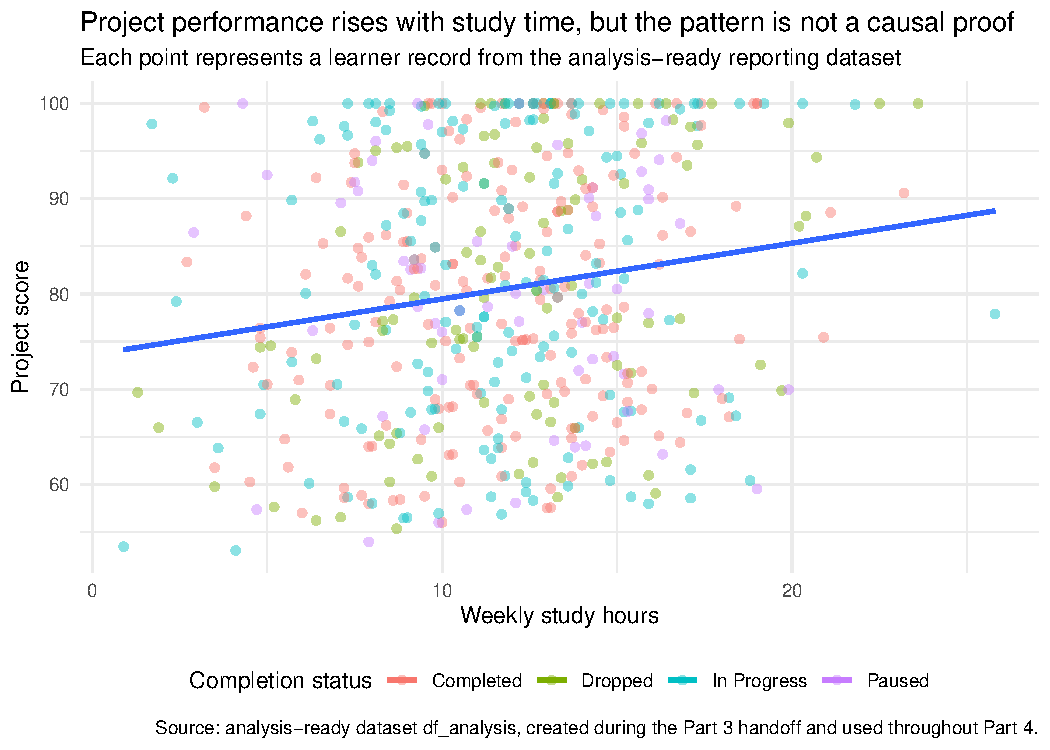
\includegraphics[width=0.9\linewidth,height=\textheight,keepaspectratio,alt={Scatter plot of weekly study hours on the horizontal axis and project score on the vertical axis. Points are grouped by completion status. The figure shows the overall relationship between study time and project performance but does not establish causation.}]{chapters/19-reproducible-reports-with-quarto_files/figure-pdf/fig-19-study-project-report-1.pdf}

}

\caption{\label{fig-19-study-project-report}Weekly Study Hours and
Project Scores in the Analysis-Ready Dataset.}

\end{figure}%

Figure~\ref{fig-19-study-project-report} shows why reproducible
reporting matters after visualization. The figure is not only displayed.
It is produced by code at render time. If Leo corrects the prepared
dataset and renders again, the figure will be regenerated from the
current data.

This does not make the interpretation automatic. Leo still has to write
responsibly. The caption and title avoid a causal claim because the plot
shows association, not experimental proof. That is the Chapter 18
discipline carried into a Chapter 19 document.

\begin{tcolorbox}[enhanced jigsaw, arc=.35mm, bottomrule=.15mm, breakable, colback=white, colframe=quarto-callout-tip-color-frame, left=2mm, leftrule=.75mm, opacityback=0, rightrule=.15mm, toprule=.15mm]
\begin{minipage}[t]{5.5mm}
\textcolor{quarto-callout-tip-color}{\faLightbulb}
\end{minipage}%
\begin{minipage}[t]{\textwidth - 5.5mm}

\vspace{-3mm}\textbf{Caption before confidence}\vspace{3mm}

If Leo cannot write a clear caption for a figure, he may not yet know
what the figure is doing in the report.

\end{minipage}%
\end{tcolorbox}

\section{Cross-Referencing Tables and
Figures}\label{cross-referencing-tables-and-figures}

Cross-referencing is one of the habits that separates a professional
report from a loose collection of outputs.

A captioned table or figure can be labelled. Once labelled, it can be
referenced in prose. Instead of writing ``the table above'' or ``the
figure below,'' Leo writes a reference such as
\texttt{@tbl-19-completion-summary} or
\texttt{@fig-19-study-project-report}.

This matters because documents move. A figure that is below one
paragraph may move above it after editing. A new table may be inserted
between two sections. The phrase ``the figure below'' can become wrong.
A cross-reference remains tied to the labelled evidence.

The table in Table~\ref{tbl-19-completion-summary} and the figure in
Figure~\ref{fig-19-study-project-report} are not just visible outputs.
They are named parts of the argument. The prose can point to them
precisely.

Good cross-referencing also disciplines interpretation. It forces Leo to
connect claims to evidence.

A weak sentence says:

\begin{quote}
Learners seem to perform better with more study time.
\end{quote}

A stronger sentence says:

\begin{quote}
Figure~\ref{fig-19-study-project-report} suggests a positive association
between weekly study hours and project score, although the figure does
not establish that study time alone caused the difference.
\end{quote}

The second sentence does more analytical work. It points to the
evidence, names the pattern, and limits the claim.

\section{Hiding Code Without Hiding
Evidence}\label{hiding-code-without-hiding-evidence}

A common beginner mistake is to confuse hiding code with hiding
evidence.

In many professional reports, the reader does not need to see every line
of R code. A manager, policy colleague, supervisor, or client may need
the result, the method summary, the source, and the limitation, not the
full syntax. In that context, \texttt{echo:\ false} can be appropriate.

But the evidence must remain visible and traceable.

If Leo hides the code for a table, the table should still have a
caption. The prose should still explain what was summarised. The report
should still name the dataset and the analytical scope. If the report is
reviewed technically, Leo should be able to share the source
\texttt{.qmd} file.

The question is not, ``Should all code always be visible?'' The better
question is:

\begin{quote}
Does the report give the reader enough information to understand, trust,
and, where necessary, check the result?
\end{quote}

For a teaching chapter, showing code is often useful. For a polished
stakeholder report, hiding routine code may improve readability. For an
audit or methods appendix, showing code may be essential.

Reproducibility is not the same as visual clutter. It is the ability to
rebuild the output from the source.

\section{Rendering to HTML, PDF, and
Word}\label{rendering-to-html-pdf-and-word}

A \texttt{.qmd} file is the source document. Rendering turns that source
into an output.

The output format depends on the document or project settings. A Quarto
document may render to HTML for web reading, PDF for print-like
distribution, or Word for collaborative editing and institutional
workflows.

\begin{Shaded}
\begin{Highlighting}[]
\NormalTok{tibble}\SpecialCharTok{::}\FunctionTok{tribble}\NormalTok{(}
  \SpecialCharTok{\textasciitilde{}}\StringTok{\textasciigrave{}}\AttributeTok{Output Format}\StringTok{\textasciigrave{}}\NormalTok{, }\SpecialCharTok{\textasciitilde{}}\StringTok{\textasciigrave{}}\AttributeTok{Useful When}\StringTok{\textasciigrave{}}\NormalTok{, }\SpecialCharTok{\textasciitilde{}}\StringTok{\textasciigrave{}}\AttributeTok{Practical Note}\StringTok{\textasciigrave{}}\NormalTok{,}
  \StringTok{"HTML"}\NormalTok{, }\StringTok{"The report will be read in a browser or published online"}\NormalTok{, }\StringTok{"Good for navigation, links, and screen{-}based reading"}\NormalTok{,}
  \StringTok{"PDF"}\NormalTok{, }\StringTok{"The report needs stable pagination or print{-}like formatting"}\NormalTok{, }\StringTok{"Usually requires a working TeX setup"}\NormalTok{,}
  \StringTok{"Word"}\NormalTok{, }\StringTok{"The report must be reviewed or edited in a familiar document workflow"}\NormalTok{, }\StringTok{"Useful for supervisors, editors, and institutions that request .docx files"}
\NormalTok{) }\SpecialCharTok{|\textgreater{}}
\NormalTok{  knitr}\SpecialCharTok{::}\FunctionTok{kable}\NormalTok{()}
\end{Highlighting}
\end{Shaded}

{

\begin{longtable}[]{@{}
  >{\raggedright\arraybackslash}p{(\linewidth - 4\tabcolsep) * \real{0.0881}}
  >{\raggedright\arraybackslash}p{(\linewidth - 4\tabcolsep) * \real{0.4403}}
  >{\raggedright\arraybackslash}p{(\linewidth - 4\tabcolsep) * \real{0.4717}}@{}}

\caption{\label{tbl-19-render-formats}Common Quarto Output Formats and
Their Reporting Uses.}

\tabularnewline

\toprule\noalign{}
\begin{minipage}[b]{\linewidth}\raggedright
Output Format
\end{minipage} & \begin{minipage}[b]{\linewidth}\raggedright
Useful When
\end{minipage} & \begin{minipage}[b]{\linewidth}\raggedright
Practical Note
\end{minipage} \\
\midrule\noalign{}
\endhead
\bottomrule\noalign{}
\endlastfoot
HTML & The report will be read in a browser or published online & Good
for navigation, links, and screen-based reading \\
PDF & The report needs stable pagination or print-like formatting &
Usually requires a working TeX setup \\
Word & The report must be reviewed or edited in a familiar document
workflow & Useful for supervisors, editors, and institutions that
request .docx files \\

\end{longtable}

}

Table~\ref{tbl-19-render-formats} helps Leo choose output format by
reader need rather than habit. The same source document can often
support more than one output, although each format has its own strengths
and constraints.

Rendering can be done in RStudio or from the terminal.

\begin{codelisting}

\caption{\label{lst-19-render-commands}Common Terminal Commands for
Rendering a Quarto Report}

\centering{

\begin{Shaded}
\begin{Highlighting}[]
\ExtensionTok{quarto}\NormalTok{ render report.qmd}
\ExtensionTok{quarto}\NormalTok{ render report.qmd }\AttributeTok{{-}{-}to}\NormalTok{ html}
\ExtensionTok{quarto}\NormalTok{ render report.qmd }\AttributeTok{{-}{-}to}\NormalTok{ pdf}
\ExtensionTok{quarto}\NormalTok{ render report.qmd }\AttributeTok{{-}{-}to}\NormalTok{ docx}
\end{Highlighting}
\end{Shaded}

}

\end{codelisting}%

The commands in Listing~\ref{lst-19-render-commands} show the idea.
Rendering means Quarto reads the source \texttt{.qmd}, executes the code
chunks that should run, collects their outputs, applies the document
settings, and writes the final file.

When Leo changes the source document, he should render again. The
rendered file is an output. The \texttt{.qmd} file is the source of
truth.

\begin{tcolorbox}[enhanced jigsaw, arc=.35mm, bottomrule=.15mm, breakable, colback=white, colframe=quarto-callout-important-color-frame, left=2mm, leftrule=.75mm, opacityback=0, rightrule=.15mm, toprule=.15mm]
\begin{minipage}[t]{5.5mm}
\textcolor{quarto-callout-important-color}{\faExclamation}
\end{minipage}%
\begin{minipage}[t]{\textwidth - 5.5mm}

\vspace{-3mm}\textbf{Edit the source, not the output}\vspace{3mm}

If Leo manually edits the rendered Word, PDF, or HTML output, the change
may disappear the next time the report is rendered. Durable changes
belong in the \texttt{.qmd} source.

\end{minipage}%
\end{tcolorbox}

\section{Common Beginner Mistakes}\label{common-beginner-mistakes-10}

\subsection{Mistake 1: Treating Quarto as Word with code pasted
in}\label{mistake-1-treating-quarto-as-word-with-code-pasted-in}

Quarto is not a word processor that happens to allow code. It is a
source document that renders into a reader-facing output. Leo should
edit the \texttt{.qmd} source, not manually repair the rendered file.

\subsection{Mistake 2: Forgetting to render after
changes}\label{mistake-2-forgetting-to-render-after-changes}

Saving a \texttt{.qmd} file is not the same as rebuilding the output. If
Leo changes data, code, captions, or interpretation, he should render
again and inspect the result.

\subsection{Mistake 3: Using absolute machine-specific
paths}\label{mistake-3-using-absolute-machine-specific-paths}

A path such as \texttt{C:/Users/Leo/Desktop/report/data.csv} may work on
Leo's laptop and fail everywhere else. Project-relative paths such as
\texttt{data/processed/df\_analysis.rds} are safer for reproducible
projects.

\subsection{Mistake 4: Hiding all code without explaining the
method}\label{mistake-4-hiding-all-code-without-explaining-the-method}

A readable report may hide code, but it should not hide the analytical
logic. The reader still needs source, scope, method, and limitation.

\subsection{Mistake 5: Creating figures or tables without
captions}\label{mistake-5-creating-figures-or-tables-without-captions}

A table or figure without a caption has no professional identity.
Captions help readers understand what the output is, where it comes
from, and how far it can be used.

\subsection{Mistake 6: Failing to cross-reference evidence in
prose}\label{mistake-6-failing-to-cross-reference-evidence-in-prose}

Phrases such as ``as shown below'' can break when the document is
edited. Cross-references keep the prose tied to the correct labelled
output.

\subsection{Mistake 7: Letting chunk options obscure the
analysis}\label{mistake-7-letting-chunk-options-obscure-the-analysis}

\texttt{echo:\ false}, \texttt{include:\ false}, and
\texttt{warning:\ false} are useful options, but they must be used
deliberately. They should control communication, not hide problems.

\subsection{Mistake 8: Mixing raw and processed data without
explanation}\label{mistake-8-mixing-raw-and-processed-data-without-explanation}

Chapter 19 uses \texttt{df\_analysis} because the report begins from the
analysis-ready handoff. If Leo switches back to raw or messy data, he
must explain why and document the cleaning path.

\subsection{Mistake 9: Editing rendered output
manually}\label{mistake-9-editing-rendered-output-manually}

Manual edits to a rendered file are fragile. If the report is rendered
again, those edits may be lost. The reliable place to revise text, code,
captions, and references is the source \texttt{.qmd} file.

\section{Try It Yourself}\label{try-it-yourself-5}

\subsection{Practice 1: Build a one-page
report}\label{practice-1-build-a-one-page-report}

Create a new file called \texttt{learner-progress-report.qmd}. Give it a
title, one short introduction, one summary table, one figure, and one
conclusion paragraph.

\subsection{Practice 2: Add a captioned
table}\label{practice-2-add-a-captioned-table}

Summarise average project score by \texttt{preferred\_learning\_mode}.
Give the table a \texttt{tbl-cap}, a clear label, and one sentence that
refers to the table using a cross-reference.

\subsection{Practice 3: Add a captioned
figure}\label{practice-3-add-a-captioned-figure}

Create a plot of \texttt{study\_hours} and \texttt{project\_score}. Add
\texttt{fig-cap}, \texttt{fig-alt}, and one sentence that refers to the
figure using a cross-reference.

\subsection{Practice 4: Hide setup but not
evidence}\label{practice-4-hide-setup-but-not-evidence}

Add a setup chunk that loads packages and imports \texttt{df\_analysis}.
Use \texttt{include:\ false} for the setup chunk. Keep the table and
figure visible.

\subsection{Practice 5: Render twice}\label{practice-5-render-twice}

Render the report once. Then change one sentence in the interpretation
and render again. Notice that the final document is produced from the
source each time.

\subsection{Practice 6: Check the
claims}\label{practice-6-check-the-claims}

Find one sentence in the report that sounds too strong. Rewrite it so it
points to the table or figure and limits the claim to what the evidence
supports.

\section{A Small Practice Lab}\label{a-small-practice-lab-6}

The lab below gives Leo a compact report scaffold. It is not evaluated
automatically because it is meant to be copied into a new \texttt{.qmd}
file and rendered manually.

\begin{codelisting}

\caption{\label{lst-19-practice-lab}Code for a Small Reproducible Quarto
Report Practice Lab}

\centering{

\begin{Shaded}
\begin{Highlighting}[]
\CommentTok{\# Copy this scaffold into a new report and add prose around each output.}

\CommentTok{\# Step 1: Load the analysis{-}ready data.}
\NormalTok{df\_analysis }\OtherTok{\textless{}{-}} \FunctionTok{readRDS}\NormalTok{(}\StringTok{"data/processed/df\_analysis.rds"}\NormalTok{)}

\CommentTok{\# Step 2: Create a reader{-}facing summary table.}
\NormalTok{progress\_by\_mode }\OtherTok{\textless{}{-}}\NormalTok{ df\_analysis }\SpecialCharTok{|\textgreater{}}
  \FunctionTok{group\_by}\NormalTok{(preferred\_learning\_mode) }\SpecialCharTok{|\textgreater{}}
  \FunctionTok{summarise}\NormalTok{(}
    \AttributeTok{learners =}\NormalTok{ dplyr}\SpecialCharTok{::}\FunctionTok{n}\NormalTok{(),}
    \AttributeTok{average\_study\_hours =} \FunctionTok{mean}\NormalTok{(study\_hours, }\AttributeTok{na.rm =} \ConstantTok{TRUE}\NormalTok{),}
    \AttributeTok{average\_project\_score =} \FunctionTok{mean}\NormalTok{(project\_score, }\AttributeTok{na.rm =} \ConstantTok{TRUE}\NormalTok{),}
    \AttributeTok{.groups =} \StringTok{"drop"}
\NormalTok{  )}

\NormalTok{progress\_by\_mode }\SpecialCharTok{|\textgreater{}}
\NormalTok{  knitr}\SpecialCharTok{::}\FunctionTok{kable}\NormalTok{()}

\CommentTok{\# Step 3: Create a reader{-}facing figure.}
\NormalTok{progress\_plot }\OtherTok{\textless{}{-}} \FunctionTok{ggplot}\NormalTok{(df\_analysis, }\FunctionTok{aes}\NormalTok{(}\AttributeTok{x =}\NormalTok{ study\_hours, }\AttributeTok{y =}\NormalTok{ project\_score)) }\SpecialCharTok{+}
  \FunctionTok{geom\_point}\NormalTok{(}\AttributeTok{alpha =} \FloatTok{0.4}\NormalTok{) }\SpecialCharTok{+}
  \FunctionTok{geom\_smooth}\NormalTok{(}\AttributeTok{method =} \StringTok{"lm"}\NormalTok{, }\AttributeTok{se =} \ConstantTok{FALSE}\NormalTok{) }\SpecialCharTok{+}
  \FunctionTok{labs}\NormalTok{(}
    \AttributeTok{title =} \StringTok{"Study time and project performance move together in this sample"}\NormalTok{,}
    \AttributeTok{x =} \StringTok{"Weekly study hours"}\NormalTok{,}
    \AttributeTok{y =} \StringTok{"Project score"}
\NormalTok{  ) }\SpecialCharTok{+}
  \FunctionTok{theme\_minimal}\NormalTok{()}

\NormalTok{progress\_plot}

\CommentTok{\# Step 4: Add captions, labels, alt text, and prose cross{-}references}
\CommentTok{\# in the .qmd report before rendering.}
\end{Highlighting}
\end{Shaded}

}

\end{codelisting}%

The scaffold in Listing~\ref{lst-19-practice-lab} brings together the
main habits of the chapter: loading the prepared dataset, creating a
table, creating a figure, and surrounding both with captions, labels,
cross-references, and cautious interpretation inside the report source.

\section{Short Recap}\label{short-recap-5}

In this chapter, Leo moved from analytical outputs to reproducible
analytical documents. He saw why copy-paste reporting breaks trust when
data, code, output, and prose drift apart. He learned that Quarto keeps
those elements inside one source document that can be rendered into
HTML, PDF, or Word.

He learned the main parts of a Quarto document: YAML, Markdown prose,
and code chunks. He learned how chunk options control what readers see.
He created a captioned table and a captioned figure from
\texttt{df\_analysis}. He also learned why cross-references matter, why
hidden code is not the same as hidden evidence, and why durable edits
belong in the \texttt{.qmd} source rather than the rendered output.

Most importantly, he learned that a reproducible report is not only a
document. It is a trust structure.

\section{Leo's Notebook}\label{leos-notebook-8}

\begin{itemize}
\tightlist
\item
  A copied table can become stale without warning.
\item
  A \texttt{.qmd} file keeps code, output, and explanation together.
\item
  The rendered report is the output. The source \texttt{.qmd} file is
  where durable changes belong.
\item
  YAML identifies the document. Markdown carries the explanation. Code
  chunks run the analysis.
\item
  Chunk options should help the reader, not hide analytical problems.
\item
  A table or figure should have a caption if it is part of the report's
  evidence.
\item
  Cross-references connect claims to named evidence.
\item
  \texttt{df\_analysis} is the correct starting point for this chapter
  because it comes from the prepared Part 3 handoff.
\item
  Hiding setup code can be appropriate. Hiding the logic of a result
  without explanation is risky.
\item
  Rendering is the moment when the report rebuilds itself from the
  source.
\end{itemize}

\section{Glossary}\label{glossary-5}

\textbf{Caption}\\
A short description attached to a table or figure. A good caption
identifies what the output shows and may include source, scope, or
limitation.

\textbf{Chunk option}\\
An instruction that controls how a code chunk behaves during rendering,
such as whether code is shown, output is included, warnings are
displayed, or a figure receives a caption.

\textbf{Code chunk}\\
An executable block inside a Quarto document. In R chapters, code chunks
run R code and insert the resulting output into the rendered document.

\textbf{Cross-reference}\\
A reference in the prose that points to a labelled table, figure,
listing, section, or other numbered element. Cross-references help keep
claims tied to evidence.

\textbf{Markdown}\\
A plain-text writing format used for headings, paragraphs, links, lists,
emphasis, and other document structure.

\textbf{Output format}\\
The final type of document produced when Quarto renders a source file,
such as HTML, PDF, or Word.

\textbf{Quarto document}\\
A \texttt{.qmd} source file that can combine metadata, prose, executable
code, output, captions, and references into one reproducible document.

\textbf{Render}\\
The process by which Quarto reads a \texttt{.qmd} source file, executes
code chunks where appropriate, and produces the final output document.

\textbf{Reproducible report}\\
A report whose tables, figures, and other outputs are generated from
code in the source document, so the report can be rebuilt when data or
analysis changes.

\textbf{YAML}\\
The metadata block at the top of a Quarto document. It gives information
such as the title and, where appropriate, output settings.

\section{Chapter Outcome}\label{chapter-outcome-18}

Leo can now turn analysis into a reproducible report.

He can explain why copy-paste reporting is fragile. He can identify the
main parts of a Quarto document. He can load the analysis-ready dataset,
create a captioned table, create a captioned figure, and refer to both
in the prose. He can use chunk options deliberately. He can distinguish
the source \texttt{.qmd} file from the rendered output. He can also make
a stronger professional judgement about when to show code, when to hide
routine setup, and how to keep evidence visible even when code is not
printed in full.

This is the first threshold of Part 5.

Leo is no longer only producing analyses. He is beginning to build
analytical systems.

\section{What Comes Next}\label{what-comes-next-7}

Chapter 19 solved the problem of fragile reporting from a local
analysis-ready dataset.

But professional data work rarely stops there.

So far, Leo's report begins from \texttt{df\_analysis}, a prepared
dataset stored in the project. That is appropriate for learning
reproducible reporting. It gives him a stable source, a controlled
object, and a document that can be rerun.

The next question is different:

\begin{quote}
What happens when the data do not live neatly as one local file?
\end{quote}

Many real reports depend on data stored in databases, web services,
shared systems, or external platforms. Those data may update, require
access rules, or arrive in structures that are not as simple as a CSV
file.

Chapter 20 moves Leo into that world. It introduces data connections,
not as a departure from reproducible reporting, but as the next layer in
the same system. Once Leo can build a report that reruns from a local
prepared dataset, he is ready to ask how R connects to data beyond local
files.

\chapter{Data Connections: Moving Beyond Local
Files}\label{data-connections-moving-beyond-local-files}

\renewcommand{\thefigure}{20.\arabic{figure}}
\setcounter{figure}{0}
\renewcommand{\thetable}{20.\arabic{table}}
\setcounter{table}{0}

\section{Opening Scene: When the Data Is Not Waiting in the
Folder}\label{opening-scene-when-the-data-is-not-waiting-in-the-folder}

Leo has reached a different kind of confidence.

In Chapter 19, he learned how to place code, output, and explanation
inside one Quarto document. He no longer has to copy a table from the
console, paste a figure into a report, and hope that every paragraph
still matches the latest analysis. He can render the document and
rebuild the evidence from the source.

That is a serious professional threshold.

But the next problem arrives before the analysis begins.

The report may be reproducible, but where does the data come from?

So far, Leo has worked with data that can be placed inside the project.
A file can be stored in \texttt{data/raw/}, cleaned into
\texttt{data/processed/}, and then used as \texttt{df\_analysis} in a
reproducible report. That is the right foundation. It teaches discipline
before complexity.

Professional data work, however, does not always begin with a neat file
already waiting in \texttt{data/processed/}. The data may sit in a
shared spreadsheet maintained by several colleagues. It may be exposed
through a public URL. It may arrive from an API. It may live in a
database. It may be stored in a cloud folder where permissions change.
It may update every hour while Leo's report still needs to be defensible
next month.

The question is no longer only:

\begin{quote}
How do I import this file?
\end{quote}

The sharper question is:

\begin{quote}
How do I connect to data without making the analysis fragile?
\end{quote}

\begin{tcolorbox}[enhanced jigsaw, arc=.35mm, bottomrule=.15mm, breakable, colback=white, colframe=quarto-callout-important-color-frame, left=2mm, leftrule=.75mm, opacityback=0, rightrule=.15mm, toprule=.15mm]
\begin{minipage}[t]{5.5mm}
\textcolor{quarto-callout-important-color}{\faExclamation}
\end{minipage}%
\begin{minipage}[t]{\textwidth - 5.5mm}

\vspace{-3mm}\textbf{The central lightbulb}\vspace{3mm}

A data connection is not just a technical link to a source. It is a
controlled doorway between R and evidence that lives outside the current
project file.

\end{minipage}%
\end{tcolorbox}

This chapter is about that doorway.

The doorway matters because Chapter 20 is not a detour from the project
structure Leo has already built. It extends that structure. The official
working route remains \texttt{data/}: first captured evidence belongs in
\texttt{data/raw/}, prepared analytical objects belong in
\texttt{data/processed/}, and formal Quarto reports should state which
evidence route they use.

\begin{tcolorbox}[enhanced jigsaw, arc=.35mm, bottomrule=.15mm, breakable, colback=white, colframe=quarto-callout-tip-color-frame, left=2mm, leftrule=.75mm, opacityback=0, rightrule=.15mm, toprule=.15mm]
\begin{minipage}[t]{5.5mm}
\textcolor{quarto-callout-tip-color}{\faLightbulb}
\end{minipage}%
\begin{minipage}[t]{\textwidth - 5.5mm}

\vspace{-3mm}\textbf{Keep the route stable}\vspace{3mm}

Connected data may begin outside the project, but serious analysis
should not remain scattered outside the project. Leo's task is to decide
what should stay live, what should be captured, and where each captured
object belongs inside \texttt{data/}.

\end{minipage}%
\end{tcolorbox}

It does not try to turn Leo into a database administrator, web engineer,
or API specialist. It gives him the mental model he needs before those
tools become intimidating. The goal is controlled access to evidence:
knowing where the data lives, how R reaches it, what can go wrong, and
how to protect the reproducibility of the analysis when the source is
outside the project.

\section{What Changed After Chapter
19}\label{what-changed-after-chapter-19}

Chapter 19 changed the container of Leo's work.

Before Chapter 19, analysis, output, and explanation could easily drift
apart. A script created one thing, a document said another, and the
connection between them depended on memory. Chapter 19 corrected that by
placing the analytical logic and the reader-facing report inside one
source document.

Chapter 20 changes the starting point.

A reproducible report can still become fragile if the data source is
unstable, undocumented, or hidden behind a manual step. Leo can write a
beautiful Quarto report and still fail to reproduce the result if the
source spreadsheet has changed, if a URL is no longer available, if an
API key has expired, or if the database query was never recorded.

The lesson is direct: reproducibility does not begin at the first plot.
It begins at the first contact with evidence.

In Chapter 19, Leo asked whether the report could be rebuilt. In Chapter
20, he asks whether the data entering the report can be reached,
inspected, documented, and preserved with enough care.

\section{Why Local Files Are Not the Whole Data
World}\label{why-local-files-are-not-the-whole-data-world}

Local files are not inferior. They are often the safest teaching
foundation and, in many projects, the safest reproducibility choice.

A local file has important advantages. It can be placed in a predictable
folder. It can be inspected before analysis. It can be copied with the
project. It can be versioned or archived. It can be rendered again
without depending on an internet connection or a remote service.

But local files also have limits.

They can become stale. They may be manually downloaded without a record
of where they came from. Two people may use different copies without
noticing. A file saved on one machine may not exist on another. A report
may appear reproducible because the \texttt{.qmd} file renders on Leo's
laptop, while the underlying source file is actually a private download
that nobody else can access.

Connected data solves some of these problems and introduces others.

A connection can reach current data. It can reduce manual downloading.
It can pull only the needed rows from a larger source. It can support
recurring reports. It can also fail, change, require permission, return
a new structure, or silently update the evidence behind the same code.

That is why this chapter does not celebrate connected data as
automatically better. It teaches connected data as a responsibility.

\section{Local Files and Connected
Data}\label{local-files-and-connected-data}

The difference between a local file and connected data is not only
technical. It changes the logic of trust.

With a local file, Leo usually asks:

\begin{itemize}
\tightlist
\item
  Where is the file?
\item
  Can R read it?
\item
  What columns and types did R create?
\item
  Should it live in \texttt{data/raw/} or \texttt{data/processed/}?
\end{itemize}

With connected data, he must add further questions:

\begin{itemize}
\tightlist
\item
  Who controls the source?
\item
  Can the source change between renders?
\item
  Does access require credentials?
\item
  Is the connection stable enough for a reproducible report?
\item
  Should the connected result be saved as a documented snapshot?
\item
  If the data updates, does the report need freshness or reproducibility
  more urgently?
\end{itemize}

This last question is crucial.

Freshness and reproducibility are related, but they are not the same.

A live connection may give Leo the newest data. A saved snapshot may
give him the same data each time the report is rendered. Neither choice
is universally correct. The professional task is to decide which one the
analysis requires and to state that decision clearly.

This is where Leo must separate \textbf{source access} from
\textbf{analytical evidence}. Source access means R can reach a place
where data lives. Analytical evidence means the specific version of data
used to support a claim has been identified, inspected, and controlled.
A connection gives access. A documented workflow turns access into
evidence.

\begin{tcolorbox}[enhanced jigsaw, arc=.35mm, bottomrule=.15mm, breakable, colback=white, colframe=quarto-callout-note-color-frame, left=2mm, leftrule=.75mm, opacityback=0, rightrule=.15mm, toprule=.15mm]
\begin{minipage}[t]{5.5mm}
\textcolor{quarto-callout-note-color}{\faInfo}
\end{minipage}%
\begin{minipage}[t]{\textwidth - 5.5mm}

\vspace{-3mm}\textbf{Freshness is not the same as reproducibility}\vspace{3mm}

A live connection asks, ``What is the source saying now?'' A saved
snapshot asks, ``What evidence did this analysis use?'' Many
professional workflows need both, but they should not be confused.

\end{minipage}%
\end{tcolorbox}

\section{Different Doors Into Data}\label{different-doors-into-data}

Leo can now think of data sources as doors. Each door opens in a
different way, carries different risks, and demands a different habit of
control.

The comparison in Table~\ref{tbl-20-data-doors} gives him a first map.
It is not a full catalogue of every possible source. It is a practical
orientation for a learner who already understands local import and
reproducible reporting.

\begin{Shaded}
\begin{Highlighting}[]
\NormalTok{data\_doors }\OtherTok{\textless{}{-}}\NormalTok{ tibble}\SpecialCharTok{::}\FunctionTok{tribble}\NormalTok{(}
  \SpecialCharTok{\textasciitilde{}}\StringTok{\textasciigrave{}}\AttributeTok{Data door}\StringTok{\textasciigrave{}}\NormalTok{, }\SpecialCharTok{\textasciitilde{}}\StringTok{\textasciigrave{}}\AttributeTok{What Leo is accessing}\StringTok{\textasciigrave{}}\NormalTok{, }\SpecialCharTok{\textasciitilde{}}\StringTok{\textasciigrave{}}\AttributeTok{Typical R pattern}\StringTok{\textasciigrave{}}\NormalTok{, }\SpecialCharTok{\textasciitilde{}}\StringTok{\textasciigrave{}}\AttributeTok{Main reproducibility risk}\StringTok{\textasciigrave{}}\NormalTok{, }\SpecialCharTok{\textasciitilde{}}\StringTok{\textasciigrave{}}\AttributeTok{Safe beginner habit}\StringTok{\textasciigrave{}}\NormalTok{,}
  \StringTok{"Local project file"}\NormalTok{, }\StringTok{"A CSV, XLSX, or RDS file stored inside the project"}\NormalTok{, }\StringTok{"Read from \textasciigrave{}data/raw/\textasciigrave{} or \textasciigrave{}data/processed/\textasciigrave{}"}\NormalTok{, }\StringTok{"The file may be replaced without documentation"}\NormalTok{, }\StringTok{"Keep raw and processed files separate, and document the source"}\NormalTok{,}
  \StringTok{"Public URL"}\NormalTok{, }\StringTok{"A file or table available through a web address"}\NormalTok{, }\StringTok{"Read from a URL, then inspect the result"}\NormalTok{, }\StringTok{"The address may change, disappear, or return different content"}\NormalTok{, }\StringTok{"Save a dated snapshot when the result supports analysis"}\NormalTok{,}
  \StringTok{"Shared spreadsheet"}\NormalTok{, }\StringTok{"A table edited by one or more people online"}\NormalTok{, }\StringTok{"Read through an online spreadsheet package or exported CSV link"}\NormalTok{, }\StringTok{"Cells may change between renders and permissions may fail"}\NormalTok{, }\StringTok{"Agree on a snapshot point before formal analysis"}\NormalTok{,}
  \StringTok{"API"}\NormalTok{, }\StringTok{"A service that returns data after a structured request"}\NormalTok{, }\StringTok{"Send a request, receive a structured response"}\NormalTok{, }\StringTok{"Responses can change, rate limits may apply, and keys may expire"}\NormalTok{, }\StringTok{"Record the request and cache important responses"}\NormalTok{,}
  \StringTok{"Database"}\NormalTok{, }\StringTok{"Structured tables stored in a managed data system"}\NormalTok{, }\StringTok{"Open a connection, query, collect results, disconnect"}\NormalTok{, }\StringTok{"Queries may be undocumented or the database may change"}\NormalTok{, }\StringTok{"Save the query and preserve the extracted analytical result"}\NormalTok{,}
  \StringTok{"Cloud file"}\NormalTok{, }\StringTok{"A file stored outside the local project in a shared location"}\NormalTok{, }\StringTok{"Sync or download into the project route"}\NormalTok{, }\StringTok{"Local and remote copies may drift apart"}\NormalTok{, }\StringTok{"Treat the project copy as the analytical evidence"}
\NormalTok{)}

\NormalTok{data\_doors }\SpecialCharTok{|\textgreater{}}
\NormalTok{  knitr}\SpecialCharTok{::}\FunctionTok{kable}\NormalTok{()}
\end{Highlighting}
\end{Shaded}

{

\begin{longtable}[]{@{}
  >{\raggedright\arraybackslash}p{(\linewidth - 8\tabcolsep) * \real{0.0699}}
  >{\raggedright\arraybackslash}p{(\linewidth - 8\tabcolsep) * \real{0.2243}}
  >{\raggedright\arraybackslash}p{(\linewidth - 8\tabcolsep) * \real{0.2353}}
  >{\raggedright\arraybackslash}p{(\linewidth - 8\tabcolsep) * \real{0.2390}}
  >{\raggedright\arraybackslash}p{(\linewidth - 8\tabcolsep) * \real{0.2316}}@{}}

\caption{\label{tbl-20-data-doors}Common Data Doors Beyond the Current
Project File.}

\tabularnewline

\toprule\noalign{}
\begin{minipage}[b]{\linewidth}\raggedright
Data door
\end{minipage} & \begin{minipage}[b]{\linewidth}\raggedright
What Leo is accessing
\end{minipage} & \begin{minipage}[b]{\linewidth}\raggedright
Typical R pattern
\end{minipage} & \begin{minipage}[b]{\linewidth}\raggedright
Main reproducibility risk
\end{minipage} & \begin{minipage}[b]{\linewidth}\raggedright
Safe beginner habit
\end{minipage} \\
\midrule\noalign{}
\endhead
\bottomrule\noalign{}
\endlastfoot
Local project file & A CSV, XLSX, or RDS file stored inside the project
& Read from \texttt{data/raw/} or \texttt{data/processed/} & The file
may be replaced without documentation & Keep raw and processed files
separate, and document the source \\
Public URL & A file or table available through a web address & Read from
a URL, then inspect the result & The address may change, disappear, or
return different content & Save a dated snapshot when the result
supports analysis \\
Shared spreadsheet & A table edited by one or more people online & Read
through an online spreadsheet package or exported CSV link & Cells may
change between renders and permissions may fail & Agree on a snapshot
point before formal analysis \\
API & A service that returns data after a structured request & Send a
request, receive a structured response & Responses can change, rate
limits may apply, and keys may expire & Record the request and cache
important responses \\
Database & Structured tables stored in a managed data system & Open a
connection, query, collect results, disconnect & Queries may be
undocumented or the database may change & Save the query and preserve
the extracted analytical result \\
Cloud file & A file stored outside the local project in a shared
location & Sync or download into the project route & Local and remote
copies may drift apart & Treat the project copy as the analytical
evidence \\

\end{longtable}

}

The key word in Table~\ref{tbl-20-data-doors} is not \emph{external}. It
is \emph{controlled}. A URL is not useful because it is modern. A
database is not trustworthy because it is large. An API is not
professional because it sounds technical. Each source becomes useful
only when Leo can explain how the data entered the project, what version
of the evidence was analysed, and what might change later.

\section{Reading Data from a URL}\label{reading-data-from-a-url}

A URL is often the first data connection learners meet after local
files. It looks simple because it resembles file import. Instead of
reading from a path such as \texttt{data/raw/example.csv}, R reads from
a web address.

Conceptually, the movement is familiar:

\begin{enumerate}
\def\labelenumi{\arabic{enumi}.}
\tightlist
\item
  identify the source;
\item
  ask R to read it;
\item
  inspect the object R creates;
\item
  decide whether to save a local snapshot;
\item
  analyse the controlled object, not the mystery of the web address.
\end{enumerate}

The template in Listing~\ref{lst-20-read-url-csv} shows the pattern. It
is deliberately marked \texttt{eval:\ false} because live web sources
can fail during rendering. That is not a weakness in the lesson. It is
the lesson.

\begin{codelisting}

\caption{\label{lst-20-read-url-csv}Template for Reading a CSV File from
a Public URL}

\centering{

\begin{Shaded}
\begin{Highlighting}[]
\NormalTok{source\_url }\OtherTok{\textless{}{-}} \StringTok{"https://example.org/path/to/public{-}data.csv"}

\NormalTok{url\_data }\OtherTok{\textless{}{-}} \FunctionTok{read.csv}\NormalTok{(}
\NormalTok{  source\_url,}
  \AttributeTok{stringsAsFactors =} \ConstantTok{FALSE}\NormalTok{,}
  \AttributeTok{na.strings =} \FunctionTok{c}\NormalTok{(}\StringTok{""}\NormalTok{, }\StringTok{"NA"}\NormalTok{, }\StringTok{"N/A"}\NormalTok{, }\StringTok{"missing"}\NormalTok{, }\StringTok{"not available"}\NormalTok{)}
\NormalTok{)}

\FunctionTok{head}\NormalTok{(url\_data)}
\FunctionTok{str}\NormalTok{(url\_data)}
\FunctionTok{summary}\NormalTok{(url\_data)}
\end{Highlighting}
\end{Shaded}

}

\end{codelisting}%

The most important part of Listing~\ref{lst-20-read-url-csv} is not the
URL. It is the inspection after import. Leo does not treat connected
data as trustworthy merely because R successfully read it. The same
discipline from Chapter 11 still applies: inspect names, types, missing
values, row counts, and obvious structural surprises before using the
result as evidence.

A useful beginner rule is this: if the connected result matters to the
argument of the report, do not let it remain invisible. Name the source,
inspect the object, and decide whether the result should be saved.

The URL is only the access route. It is not, by itself, a method. The
method begins when Leo records where the data came from, when it was
accessed, what R received, what checks were performed, and which saved
object became the basis of the analysis.

\begin{tcolorbox}[enhanced jigsaw, arc=.35mm, bottomrule=.15mm, breakable, colback=white, colframe=quarto-callout-warning-color-frame, left=2mm, leftrule=.75mm, opacityback=0, rightrule=.15mm, toprule=.15mm]
\begin{minipage}[t]{5.5mm}
\textcolor{quarto-callout-warning-color}{\faExclamationTriangle}
\end{minipage}%
\begin{minipage}[t]{\textwidth - 5.5mm}

\vspace{-3mm}\textbf{Do not build a serious report on an invisible download}\vspace{3mm}

If Leo reads from a URL and immediately creates conclusions, he has
skipped the evidence checkpoint. A connection should be inspected before
it becomes analysis.

\end{minipage}%
\end{tcolorbox}

\section{A Safer Pattern: Connect, Inspect, Save
Deliberately}\label{a-safer-pattern-connect-inspect-save-deliberately}

Connected data often needs a two-step professional pattern.

First, Leo connects to the external source and inspects what arrives.
Second, he saves a local copy only when doing so supports
reproducibility, auditability, or careful downstream cleaning. This does
not mean every live source must be copied every time. It means the
choice must be deliberate.

The pattern in Listing~\ref{lst-20-save-snapshot-pattern} shows a
cautious route. It uses \texttt{data/raw/} for the first captured
version of evidence because the connected result has not yet been
cleaned or transformed. The file-writing lines are kept
\texttt{eval:\ false} because a chapter render should not unexpectedly
create or overwrite project files.

\begin{codelisting}

\caption{\label{lst-20-save-snapshot-pattern}A Safe Connect, Inspect,
and Snapshot Pattern}

\centering{

\begin{Shaded}
\begin{Highlighting}[]
\NormalTok{source\_url }\OtherTok{\textless{}{-}} \StringTok{"https://example.org/path/to/public{-}data.csv"}

\NormalTok{connected\_raw }\OtherTok{\textless{}{-}} \FunctionTok{read.csv}\NormalTok{(}
\NormalTok{  source\_url,}
  \AttributeTok{stringsAsFactors =} \ConstantTok{FALSE}\NormalTok{,}
  \AttributeTok{na.strings =} \FunctionTok{c}\NormalTok{(}\StringTok{""}\NormalTok{, }\StringTok{"NA"}\NormalTok{, }\StringTok{"N/A"}\NormalTok{, }\StringTok{"missing"}\NormalTok{, }\StringTok{"not available"}\NormalTok{)}
\NormalTok{)}

\CommentTok{\# Inspect before trusting.}
\FunctionTok{head}\NormalTok{(connected\_raw)}
\FunctionTok{str}\NormalTok{(connected\_raw)}
\FunctionTok{names}\NormalTok{(connected\_raw)}
\FunctionTok{summary}\NormalTok{(connected\_raw)}

\CommentTok{\# Save a documented raw snapshot when the data supports analysis.}
\FunctionTok{dir.create}\NormalTok{(}\StringTok{"data/raw"}\NormalTok{, }\AttributeTok{recursive =} \ConstantTok{TRUE}\NormalTok{, }\AttributeTok{showWarnings =} \ConstantTok{FALSE}\NormalTok{)}

\NormalTok{snapshot\_date }\OtherTok{\textless{}{-}} \FunctionTok{format}\NormalTok{(}\FunctionTok{Sys.Date}\NormalTok{(), }\StringTok{"\%Y{-}\%m{-}\%d"}\NormalTok{)}
\NormalTok{snapshot\_path }\OtherTok{\textless{}{-}} \FunctionTok{paste0}\NormalTok{(}\StringTok{"data/raw/connected\_source\_"}\NormalTok{, snapshot\_date, }\StringTok{".csv"}\NormalTok{)}

\FunctionTok{write.csv}\NormalTok{(connected\_raw, snapshot\_path, }\AttributeTok{row.names =} \ConstantTok{FALSE}\NormalTok{)}

\CommentTok{\# Save a small source note beside the snapshot.}
\NormalTok{source\_note }\OtherTok{\textless{}{-}}\NormalTok{ tibble}\SpecialCharTok{::}\FunctionTok{tibble}\NormalTok{(}
  \AttributeTok{source\_name =} \StringTok{"Public learner progress CSV"}\NormalTok{,}
  \AttributeTok{source\_url =}\NormalTok{ source\_url,}
  \AttributeTok{extraction\_date =}\NormalTok{ snapshot\_date,}
  \AttributeTok{raw\_snapshot\_path =}\NormalTok{ snapshot\_path,}
  \AttributeTok{notes =} \StringTok{"Captured before cleaning or transformation."}
\NormalTok{)}

\FunctionTok{write.csv}\NormalTok{(}
\NormalTok{  source\_note,}
  \FunctionTok{paste0}\NormalTok{(}\StringTok{"data/raw/connected\_source\_note\_"}\NormalTok{, snapshot\_date, }\StringTok{".csv"}\NormalTok{),}
  \AttributeTok{row.names =} \ConstantTok{FALSE}
\NormalTok{)}
\end{Highlighting}
\end{Shaded}

}

\end{codelisting}%

The snapshot pattern in Listing~\ref{lst-20-save-snapshot-pattern}
protects Leo from a common trap. A live source can change while the
wording of a report stays the same. Saving a snapshot gives the analysis
a known evidential base, while the source note records how that evidence
entered the project. The source can still be updated later, but the
report can state which version was used, when it was captured, and where
the captured file lives.

A source note does not need to be long, but it must answer the questions
that protect the evidence trail. The minimum fields in
Table~\ref{tbl-20-source-note-fields} give Leo a practical checklist for
documenting connected data before it becomes part of a serious report.

\begin{Shaded}
\begin{Highlighting}[]
\NormalTok{source\_note\_fields }\OtherTok{\textless{}{-}}\NormalTok{ tibble}\SpecialCharTok{::}\FunctionTok{tribble}\NormalTok{(}
  \SpecialCharTok{\textasciitilde{}}\StringTok{\textasciigrave{}}\AttributeTok{Field}\StringTok{\textasciigrave{}}\NormalTok{, }\SpecialCharTok{\textasciitilde{}}\StringTok{\textasciigrave{}}\AttributeTok{Question it answers}\StringTok{\textasciigrave{}}\NormalTok{, }\SpecialCharTok{\textasciitilde{}}\StringTok{\textasciigrave{}}\AttributeTok{Example}\StringTok{\textasciigrave{}}\NormalTok{,}
  \StringTok{"Source name"}\NormalTok{, }\StringTok{"What source did the data come from?"}\NormalTok{, }\StringTok{"Public learner progress CSV"}\NormalTok{,}
  \StringTok{"Source location"}\NormalTok{, }\StringTok{"Where was the source accessed?"}\NormalTok{, }\StringTok{"URL, sheet link, database name, or API endpoint"}\NormalTok{,}
  \StringTok{"Extraction date"}\NormalTok{, }\StringTok{"When did this version enter the project?"}\NormalTok{, }\StringTok{"2026{-}06{-}02"}\NormalTok{,}
  \StringTok{"Access method"}\NormalTok{, }\StringTok{"How did R or the analyst reach the source?"}\NormalTok{, }\StringTok{"CSV URL, shared spreadsheet, API request, SQL query"}\NormalTok{,}
  \StringTok{"Raw snapshot path"}\NormalTok{, }\StringTok{"Where was the first captured version saved?"}\NormalTok{, }\StringTok{"data/raw/connected\_source\_2026{-}06{-}02.csv"}\NormalTok{,}
  \StringTok{"Processed object path"}\NormalTok{, }\StringTok{"Where is the analysis{-}ready version stored?"}\NormalTok{, }\StringTok{"data/processed/connected\_analysis.csv"}\NormalTok{,}
  \StringTok{"Known limitations"}\NormalTok{, }\StringTok{"What should readers know before trusting the evidence?"}\NormalTok{, }\StringTok{"Columns may change in future source updates"}
\NormalTok{)}

\NormalTok{source\_note\_fields }\SpecialCharTok{|\textgreater{}}
\NormalTok{  knitr}\SpecialCharTok{::}\FunctionTok{kable}\NormalTok{()}
\end{Highlighting}
\end{Shaded}

{

\begin{longtable}[]{@{}
  >{\raggedright\arraybackslash}p{(\linewidth - 4\tabcolsep) * \real{0.1705}}
  >{\raggedright\arraybackslash}p{(\linewidth - 4\tabcolsep) * \real{0.4264}}
  >{\raggedright\arraybackslash}p{(\linewidth - 4\tabcolsep) * \real{0.4031}}@{}}

\caption{\label{tbl-20-source-note-fields}Minimum Source-Note Fields for
Connected Data.}

\tabularnewline

\toprule\noalign{}
\begin{minipage}[b]{\linewidth}\raggedright
Field
\end{minipage} & \begin{minipage}[b]{\linewidth}\raggedright
Question it answers
\end{minipage} & \begin{minipage}[b]{\linewidth}\raggedright
Example
\end{minipage} \\
\midrule\noalign{}
\endhead
\bottomrule\noalign{}
\endlastfoot
Source name & What source did the data come from? & Public learner
progress CSV \\
Source location & Where was the source accessed? & URL, sheet link,
database name, or API endpoint \\
Extraction date & When did this version enter the project? &
2026-06-02 \\
Access method & How did R or the analyst reach the source? & CSV URL,
shared spreadsheet, API request, SQL query \\
Raw snapshot path & Where was the first captured version saved? &
data/raw/connected\_source\_2026-06-02.csv \\
Processed object path & Where is the analysis-ready version stored? &
data/processed/connected\_analysis.csv \\
Known limitations & What should readers know before trusting the
evidence? & Columns may change in future source updates \\

\end{longtable}

}

This is not a retreat from connected data. It is a way to make connected
data accountable. Once Leo can name the source, the access route, the
capture date, and the saved project object, connected data begins to
behave like evidence rather than a moving target.

\section{A Small Workflow Map}\label{a-small-workflow-map}

The workflow in Figure~\ref{fig-20-connection-workflow} shows the safest
beginner movement from an outside source into a reproducible report. The
source may be live, but the analytical evidence should become visible,
inspected, and placed under project discipline before it carries a
claim.

\begin{Shaded}
\begin{Highlighting}[]
\NormalTok{workflow\_nodes }\OtherTok{\textless{}{-}}\NormalTok{ tibble}\SpecialCharTok{::}\FunctionTok{tibble}\NormalTok{(}
  \AttributeTok{step =} \DecValTok{1}\SpecialCharTok{:}\DecValTok{6}\NormalTok{,}
  \AttributeTok{stage =} \FunctionTok{factor}\NormalTok{(}
    \FunctionTok{c}\NormalTok{(}
      \StringTok{"External}\SpecialCharTok{\textbackslash{}n}\StringTok{source"}\NormalTok{,}
      \StringTok{"R}\SpecialCharTok{\textbackslash{}n}\StringTok{connection"}\NormalTok{,}
      \StringTok{"Inspect}\SpecialCharTok{\textbackslash{}n}\StringTok{structure"}\NormalTok{,}
      \StringTok{"Snapshot}\SpecialCharTok{\textbackslash{}n}\StringTok{or cache"}\NormalTok{,}
      \StringTok{"Analysis{-}ready}\SpecialCharTok{\textbackslash{}n}\StringTok{data"}\NormalTok{,}
      \StringTok{"Quarto}\SpecialCharTok{\textbackslash{}n}\StringTok{report"}
\NormalTok{    ),}
    \AttributeTok{levels =} \FunctionTok{c}\NormalTok{(}
      \StringTok{"External}\SpecialCharTok{\textbackslash{}n}\StringTok{source"}\NormalTok{,}
      \StringTok{"R}\SpecialCharTok{\textbackslash{}n}\StringTok{connection"}\NormalTok{,}
      \StringTok{"Inspect}\SpecialCharTok{\textbackslash{}n}\StringTok{structure"}\NormalTok{,}
      \StringTok{"Snapshot}\SpecialCharTok{\textbackslash{}n}\StringTok{or cache"}\NormalTok{,}
      \StringTok{"Analysis{-}ready}\SpecialCharTok{\textbackslash{}n}\StringTok{data"}\NormalTok{,}
      \StringTok{"Quarto}\SpecialCharTok{\textbackslash{}n}\StringTok{report"}
\NormalTok{    )}
\NormalTok{  ),}
  \AttributeTok{x =} \DecValTok{1}\SpecialCharTok{:}\DecValTok{6}\NormalTok{,}
  \AttributeTok{y =} \DecValTok{0}
\NormalTok{)}

\NormalTok{workflow\_arrows }\OtherTok{\textless{}{-}}\NormalTok{ tibble}\SpecialCharTok{::}\FunctionTok{tibble}\NormalTok{(}
  \AttributeTok{x =} \DecValTok{1}\SpecialCharTok{:}\DecValTok{5}\NormalTok{,}
  \AttributeTok{xend =} \DecValTok{2}\SpecialCharTok{:}\DecValTok{6}\NormalTok{,}
  \AttributeTok{y =} \DecValTok{0}\NormalTok{,}
  \AttributeTok{yend =} \DecValTok{0}
\NormalTok{)}

\FunctionTok{ggplot}\NormalTok{() }\SpecialCharTok{+}
  \FunctionTok{geom\_segment}\NormalTok{(}
    \AttributeTok{data =}\NormalTok{ workflow\_arrows,}
    \FunctionTok{aes}\NormalTok{(}\AttributeTok{x =}\NormalTok{ x }\SpecialCharTok{+} \FloatTok{0.18}\NormalTok{, }\AttributeTok{xend =}\NormalTok{ xend }\SpecialCharTok{{-}} \FloatTok{0.18}\NormalTok{, }\AttributeTok{y =}\NormalTok{ y, }\AttributeTok{yend =}\NormalTok{ yend),}
    \AttributeTok{arrow =}\NormalTok{ grid}\SpecialCharTok{::}\FunctionTok{arrow}\NormalTok{(}\AttributeTok{length =}\NormalTok{ grid}\SpecialCharTok{::}\FunctionTok{unit}\NormalTok{(}\FloatTok{0.08}\NormalTok{, }\StringTok{"inches"}\NormalTok{), }\AttributeTok{type =} \StringTok{"closed"}\NormalTok{),}
    \AttributeTok{linewidth =} \FloatTok{0.4}
\NormalTok{  ) }\SpecialCharTok{+}
  \FunctionTok{geom\_point}\NormalTok{(}
    \AttributeTok{data =}\NormalTok{ workflow\_nodes,}
    \FunctionTok{aes}\NormalTok{(}\AttributeTok{x =}\NormalTok{ x, }\AttributeTok{y =}\NormalTok{ y),}
    \AttributeTok{size =} \DecValTok{7}
\NormalTok{  ) }\SpecialCharTok{+}
  \FunctionTok{geom\_text}\NormalTok{(}
    \AttributeTok{data =}\NormalTok{ workflow\_nodes,}
    \FunctionTok{aes}\NormalTok{(}\AttributeTok{x =}\NormalTok{ x, }\AttributeTok{y =}\NormalTok{ y, }\AttributeTok{label =}\NormalTok{ stage),}
    \AttributeTok{nudge\_y =} \SpecialCharTok{{-}}\FloatTok{0.18}\NormalTok{,}
    \AttributeTok{size =} \FloatTok{3.4}\NormalTok{,}
    \AttributeTok{lineheight =} \FloatTok{0.9}
\NormalTok{  ) }\SpecialCharTok{+}
  \FunctionTok{coord\_cartesian}\NormalTok{(}\AttributeTok{xlim =} \FunctionTok{c}\NormalTok{(}\FloatTok{0.6}\NormalTok{, }\FloatTok{6.4}\NormalTok{), }\AttributeTok{ylim =} \FunctionTok{c}\NormalTok{(}\SpecialCharTok{{-}}\FloatTok{0.55}\NormalTok{, }\FloatTok{0.35}\NormalTok{)) }\SpecialCharTok{+}
  \FunctionTok{labs}\NormalTok{(}
    \AttributeTok{title =} \StringTok{"Connected data becomes report evidence only after control steps"}\NormalTok{,}
    \AttributeTok{caption =}\NormalTok{ chapter20\_caption\_source}
\NormalTok{  ) }\SpecialCharTok{+}
  \FunctionTok{theme\_void}\NormalTok{() }\SpecialCharTok{+}
  \FunctionTok{theme}\NormalTok{(}
    \AttributeTok{plot.title =} \FunctionTok{element\_text}\NormalTok{(}\AttributeTok{hjust =} \FloatTok{0.5}\NormalTok{),}
    \AttributeTok{plot.caption =} \FunctionTok{element\_text}\NormalTok{(}\AttributeTok{hjust =} \FloatTok{0.5}\NormalTok{)}
\NormalTok{  )}
\end{Highlighting}
\end{Shaded}

\begin{figure}[H]

\centering{

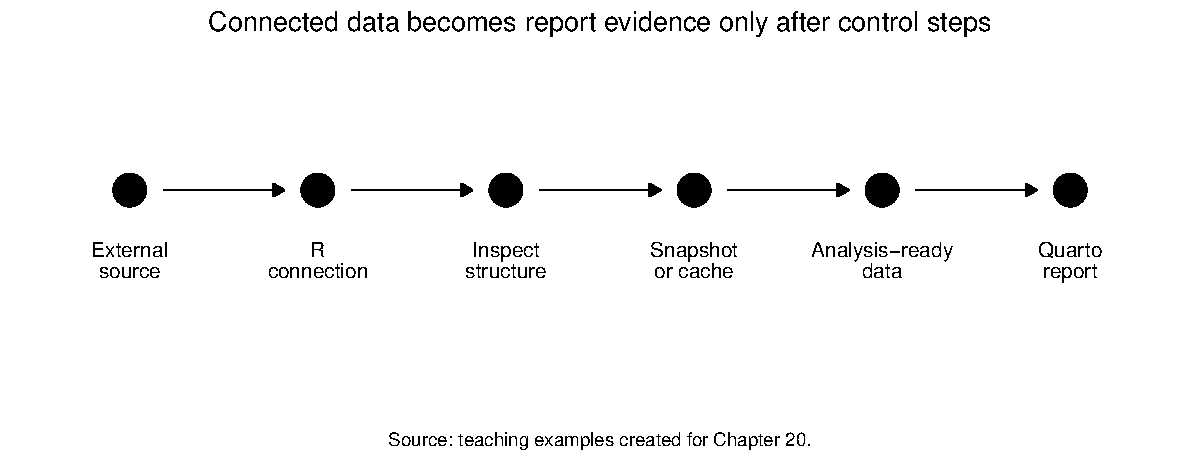
\includegraphics[width=0.9\linewidth,height=\textheight,keepaspectratio,alt={A horizontal workflow diagram with six stages: external source, R connection, inspect structure, save snapshot or cache, analysis-ready data, and Quarto report. The figure emphasises that connected data should pass through inspection and project control before becoming report evidence.}]{chapters/20-data-connections_files/figure-pdf/fig-20-connection-workflow-1.pdf}

}

\caption{\label{fig-20-connection-workflow}A Controlled Workflow for
Moving from Connected Data to a Reproducible Report.}

\end{figure}%

Figure~\ref{fig-20-connection-workflow} is intentionally simple. It does
not show every possible technology. It shows the habit that matters
across technologies: external data should pass through a controlled
pathway before it becomes a table, figure, or conclusion in a Quarto
report.

\section{Online Spreadsheets as Shared Data
Sources}\label{online-spreadsheets-as-shared-data-sources}

Shared spreadsheets are attractive because they feel familiar. Many
teams already use them to collect records, update categories, or review
status fields. For Leo, this can feel like a bridge between Excel-based
work and reproducible R workflows.

The risk is that shared spreadsheets are easy to change.

A colleague may correct a value. Another may rename a column. Someone
may filter a view and mistake the view for the whole dataset. A sheet
that rendered yesterday may require permission today. None of these
problems make shared spreadsheets unusable. They make documentation
essential.

The optional pattern in Listing~\ref{lst-20-google-sheets-template}
shows the idea without requiring credentials during rendering. It keeps
the demonstration as a template because online spreadsheet access
depends on package setup, permissions, and the sharing status of the
sheet.

\begin{codelisting}

\caption{\label{lst-20-google-sheets-template}Optional Template for
Reading a Shared Online Spreadsheet}

\centering{

\begin{Shaded}
\begin{Highlighting}[]
\CommentTok{\# install.packages("googlesheets4") library(googlesheets4) \# Use this only for public sheets that do not require private access. googlesheets4::gs4\_deauth() sheet\_url \textless{}{-} "https://docs.google.com/spreadsheets/d/example{-}sheet{-}id" shared\_sheet \textless{}{-} googlesheets4::read\_sheet(sheet\_url)}

\CommentTok{\# Always inspect the result before using it.}
\FunctionTok{glimpse}\NormalTok{(shared\_sheet)}
\FunctionTok{count}\NormalTok{(shared\_sheet, completion\_status)}
\end{Highlighting}
\end{Shaded}

}

\end{codelisting}%

The point of Listing~\ref{lst-20-google-sheets-template} is not that
every reader must use Google Sheets. The point is broader: a shared
spreadsheet is not automatically an analysis-ready dataset. A public
sheet may be readable without authentication, while a private or
institutional sheet may require approved access. In both cases, Leo
should treat the sheet as a source, inspect what arrives, and decide
whether a snapshot belongs in \texttt{data/raw/} before the cleaning and
preparation workflow begins.

A practical rule helps: a shared spreadsheet can be a collection space,
but a documented project file should become the analytical evidence for
serious reporting.

\section{APIs Without the Mystery}\label{apis-without-the-mystery}

An API is often described in language that makes it sound more difficult
than it is. Leo does not need to master web engineering to understand
the basic idea.

An API is a structured way for one system to ask another system for
something.

R sends a request. The service returns a response. The response may
include data, metadata, status information, or an error message. Many
APIs return JSON, a structured text format that can represent lists,
names, values, and nested objects.

For beginner purposes, Leo can hold four ideas:

\begin{itemize}
\tightlist
\item
  A \textbf{request} is what R asks for.
\item
  A \textbf{response} is what the service sends back.
\item
  A \textbf{status code} tells whether the request succeeded, failed, or
  needs attention.
\item
  A \textbf{rate limit} controls how often the service allows requests.
\end{itemize}

Some APIs are public. Others require keys or tokens. Those keys are not
decoration. They are access credentials. Leo should never paste them
directly into a Quarto chapter, Git repository, or shared script.

The template in Listing~\ref{lst-20-api-template} keeps the pattern
conceptual. It uses environment variables for credentials and keeps
execution off because real APIs vary in endpoint structure,
authentication rules, response formats, and rate limits.

\begin{codelisting}

\caption{\label{lst-20-api-template}Conceptual API Request Pattern Using
an Environment Variable}

\centering{

\begin{Shaded}
\begin{Highlighting}[]
\CommentTok{\# install.packages(c("httr2", "jsonlite"))}
\FunctionTok{library}\NormalTok{(httr2)}
\FunctionTok{library}\NormalTok{(jsonlite)}

\NormalTok{api\_key }\OtherTok{\textless{}{-}} \FunctionTok{Sys.getenv}\NormalTok{(}\StringTok{"MY\_SERVICE\_API\_KEY"}\NormalTok{)}

\ControlFlowTok{if}\NormalTok{ (}\FunctionTok{identical}\NormalTok{(api\_key, }\StringTok{""}\NormalTok{)) \{}
  \FunctionTok{stop}\NormalTok{(}\StringTok{"MY\_SERVICE\_API\_KEY is not available. Set it outside the .qmd file before running this request."}\NormalTok{)}
\NormalTok{\}}

\NormalTok{api\_request }\OtherTok{\textless{}{-}}\NormalTok{ httr2}\SpecialCharTok{::}\FunctionTok{request}\NormalTok{(}\StringTok{"https://api.example.org/v1/records"}\NormalTok{) }\SpecialCharTok{|\textgreater{}}
\NormalTok{  httr2}\SpecialCharTok{::}\FunctionTok{req\_headers}\NormalTok{(}\AttributeTok{Authorization =} \FunctionTok{paste}\NormalTok{(}\StringTok{"Bearer"}\NormalTok{, api\_key)) }\SpecialCharTok{|\textgreater{}}
\NormalTok{  httr2}\SpecialCharTok{::}\FunctionTok{req\_url\_query}\NormalTok{(}\AttributeTok{limit =} \DecValTok{100}\NormalTok{)}

\NormalTok{response }\OtherTok{\textless{}{-}}\NormalTok{ httr2}\SpecialCharTok{::}\FunctionTok{req\_perform}\NormalTok{(api\_request) }\CommentTok{\# Stop early if the service returned an error response. httr2::resp\_check\_status(response) response\_body \textless{}{-} httr2::resp\_body\_string(response) api\_data \textless{}{-} jsonlite::fromJSON(response\_body) str(api\_data)}
\end{Highlighting}
\end{Shaded}

}

\end{codelisting}%

Listing~\ref{lst-20-api-template} should give Leo the shape of API work
without pretending that all APIs behave identically. The safe habit is
transferable: keep credentials out of the source file, record the
request, check the response status, inspect the returned structure, and
preserve the evidence used for analysis when the result matters. In API
work, the endpoint, parameters, date of access, status outcome, and
response structure are not background details. They are part of the
method.

\begin{tcolorbox}[enhanced jigsaw, arc=.35mm, bottomrule=.15mm, breakable, colback=white, colframe=quarto-callout-warning-color-frame, left=2mm, leftrule=.75mm, opacityback=0, rightrule=.15mm, toprule=.15mm]
\begin{minipage}[t]{5.5mm}
\textcolor{quarto-callout-warning-color}{\faExclamationTriangle}
\end{minipage}%
\begin{minipage}[t]{\textwidth - 5.5mm}

\vspace{-3mm}\textbf{Never hard-code secrets}\vspace{3mm}

An API key, token, password, or private URL should not be typed directly
into a \texttt{.qmd} chapter. If the file is shared, backed up, or
committed to version control, the secret can travel with it.

\end{minipage}%
\end{tcolorbox}

\section{Databases Without the
Intimidation}\label{databases-without-the-intimidation}

A database is a managed system for storing structured data. Leo can
think of it as a place where many related tables may live, often with
rules about access, consistency, and updates.

The beginner mistake is to imagine that using a database means loading
the whole database into R. That is usually the wrong mental model.

A better model is:

\begin{quote}
connect, ask for the needed result, receive a table, close the
connection.
\end{quote}

The asking is often done through SQL. Leo does not need to become fluent
in SQL in this chapter. He only needs to understand that SQL is a query
language, a way of specifying which columns, rows, or summaries should
be returned from a database.

The optional template in Listing~\ref{lst-20-database-template} uses
\texttt{DBI} and \texttt{RSQLite} because they are common teaching tools
for database workflows in R. It remains \texttt{eval:\ false} because
optional packages should not be required for the chapter to render.

\begin{codelisting}

\caption{\label{lst-20-database-template}Optional Template for
Connecting to a Small SQLite Database}

\centering{

\begin{Shaded}
\begin{Highlighting}[]
\CommentTok{\# install.packages(c("DBI", "RSQLite"))}
\FunctionTok{library}\NormalTok{(DBI)}
\FunctionTok{library}\NormalTok{(RSQLite)}

\NormalTok{connection }\OtherTok{\textless{}{-}}\NormalTok{ DBI}\SpecialCharTok{::}\FunctionTok{dbConnect}\NormalTok{(}
\NormalTok{  RSQLite}\SpecialCharTok{::}\FunctionTok{SQLite}\NormalTok{(),}
  \StringTok{"data/raw/learner\_records.sqlite"}
\NormalTok{)}

\FunctionTok{on.exit}\NormalTok{(DBI}\SpecialCharTok{::}\FunctionTok{dbDisconnect}\NormalTok{(connection), }\AttributeTok{add =} \ConstantTok{TRUE}\NormalTok{)}

\NormalTok{learner\_summary }\OtherTok{\textless{}{-}}\NormalTok{ DBI}\SpecialCharTok{::}\FunctionTok{dbGetQuery}\NormalTok{(}
\NormalTok{  connection,}
  \StringTok{"}
\StringTok{  SELECT completion\_status,}
\StringTok{         COUNT(*) AS learners}
\StringTok{  FROM learner\_records}
\StringTok{  GROUP BY completion\_status}
\StringTok{  "}
\NormalTok{)}

\NormalTok{learner\_summary}
\end{Highlighting}
\end{Shaded}

}

\end{codelisting}%

Listing~\ref{lst-20-database-template} carries one important discipline:
the query is part of the method. If Leo extracts data from a database
but does not preserve the query, the evidence trail is incomplete. A
result table without the query that produced it is like a figure without
the code that drew it.

When the extracted result becomes the basis for a report, Leo should
decide whether to save it as a snapshot in \texttt{data/raw/} or as a
processed object in \texttt{data/processed/} after cleaning. The
database remains the source system. The saved project file becomes the
documented evidence used for a specific analysis.

\section{Credentials, Privacy, and
Access}\label{credentials-privacy-and-access}

Connected data introduces access questions that local files may hide.

Some sources are public. Some are restricted. Some are technically
reachable but ethically inappropriate to use. Some contain personal,
institutional, or sensitive information. A connection that works is not
automatically a connection Leo should use.

The first professional question is permission.

Does Leo have the right to access the source? Does he have the right to
analyse it? Does he have the right to store a local copy? Does he have
the right to share the output? These questions belong before the code,
not after the report is written.

The second question is credential handling.

A credential is a proof of access. It may be a password, token, API key,
database username, service account, or private URL. Credentials should
be stored outside the \texttt{.qmd} file and loaded securely at runtime.
Environment variables are one common pattern.

The conceptual pattern in Listing~\ref{lst-20-env-var-template} shows
the idea. The secret is read from the environment. It is not written
into the chapter.

\begin{codelisting}

\caption{\label{lst-20-env-var-template}Conceptual Pattern for Reading a
Credential from an Environment Variable}

\centering{

\begin{Shaded}
\begin{Highlighting}[]
\NormalTok{api\_key }\OtherTok{\textless{}{-}} \FunctionTok{Sys.getenv}\NormalTok{(}\StringTok{"MY\_SERVICE\_API\_KEY"}\NormalTok{)}

\ControlFlowTok{if}\NormalTok{ (}\FunctionTok{identical}\NormalTok{(api\_key, }\StringTok{""}\NormalTok{)) \{}
  \FunctionTok{stop}\NormalTok{(}\StringTok{"The API key is not available. Set MY\_SERVICE\_API\_KEY before running this code."}\NormalTok{)}
\NormalTok{\}}

\CommentTok{\# Use api\_key in the request, but do not print it.}
\end{Highlighting}
\end{Shaded}

}

\end{codelisting}%

Listing~\ref{lst-20-env-var-template} is intentionally small because the
principle matters more than the mechanics here. Do not print secrets. Do
not commit secrets. Do not hide a secret in a Quarto file and assume
nobody will see it. If secrets are stored in a local \texttt{.Renviron}
file, that file should not be casually shared or committed to a
repository. Chapter 21 will return to the danger from another angle when
Leo learns that version control remembers changes.

Privacy is broader than passwords. Even if Leo can connect to data, he
must still ask what the data contains. Learner names, staff records,
financial fields, locations, contact details, and identifiable notes
require care. A connected workflow can move sensitive data quickly,
which makes discipline more important, not less.

\section{Connected Data and
Reproducibility}\label{connected-data-and-reproducibility}

Connected data can strengthen a workflow, but it can also weaken
reproducibility if Leo does not control the evidence path. The table in
Table~\ref{tbl-20-reproducibility-risks} names the main risks and the
corresponding safeguards.

\begin{Shaded}
\begin{Highlighting}[]
\NormalTok{reproducibility\_risks }\OtherTok{\textless{}{-}}\NormalTok{ tibble}\SpecialCharTok{::}\FunctionTok{tribble}\NormalTok{(}
  \SpecialCharTok{\textasciitilde{}}\StringTok{\textasciigrave{}}\AttributeTok{Risk}\StringTok{\textasciigrave{}}\NormalTok{, }\SpecialCharTok{\textasciitilde{}}\StringTok{\textasciigrave{}}\AttributeTok{How it appears in practice}\StringTok{\textasciigrave{}}\NormalTok{, }\SpecialCharTok{\textasciitilde{}}\StringTok{\textasciigrave{}}\AttributeTok{Practical safeguard}\StringTok{\textasciigrave{}}\NormalTok{,}
  \StringTok{"Changing source"}\NormalTok{, }\StringTok{"The same URL, sheet, API, or query returns different data later"}\NormalTok{, }\StringTok{"Save a dated snapshot and record when it was captured"}\NormalTok{,}
  \StringTok{"Broken access"}\NormalTok{, }\StringTok{"A render fails because permission, internet access, or credentials are unavailable"}\NormalTok{, }\StringTok{"Separate live retrieval from formal reporting when stability matters"}\NormalTok{,}
  \StringTok{"Undocumented request"}\NormalTok{, }\StringTok{"A table exists but nobody knows which query or parameters produced it"}\NormalTok{, }\StringTok{"Store the URL, query, endpoint, parameters, and extraction date"}\NormalTok{,}
  \StringTok{"Structure drift"}\NormalTok{, }\StringTok{"A column is renamed, removed, retyped, or moved"}\NormalTok{, }\StringTok{"Inspect names and types after retrieval, and fail early when required fields are missing"}\NormalTok{,}
  \StringTok{"Hidden manual step"}\NormalTok{, }\StringTok{"A person downloads or edits data outside the recorded workflow"}\NormalTok{, }\StringTok{"Write the download, cleaning, and snapshot decisions into the project notes or code"}\NormalTok{,}
  \StringTok{"Secret leakage"}\NormalTok{, }\StringTok{"Keys or passwords are placed inside scripts or reports"}\NormalTok{, }\StringTok{"Use environment variables or approved secret management practices"}\NormalTok{,}
  \StringTok{"Confusion between live and fixed evidence"}\NormalTok{, }\StringTok{"A report claims one result but rerenders from newer data"}\NormalTok{, }\StringTok{"State clearly whether the report uses a live connection or a saved snapshot"}
\NormalTok{)}

\NormalTok{reproducibility\_risks }\SpecialCharTok{|\textgreater{}}
\NormalTok{  knitr}\SpecialCharTok{::}\FunctionTok{kable}\NormalTok{()}
\end{Highlighting}
\end{Shaded}

{

\begin{longtable}[]{@{}
  >{\raggedright\arraybackslash}p{(\linewidth - 4\tabcolsep) * \real{0.1963}}
  >{\raggedright\arraybackslash}p{(\linewidth - 4\tabcolsep) * \real{0.3879}}
  >{\raggedright\arraybackslash}p{(\linewidth - 4\tabcolsep) * \real{0.4159}}@{}}

\caption{\label{tbl-20-reproducibility-risks}Reproducibility Risks
Introduced by Connected Data and Practical Safeguards.}

\tabularnewline

\toprule\noalign{}
\begin{minipage}[b]{\linewidth}\raggedright
Risk
\end{minipage} & \begin{minipage}[b]{\linewidth}\raggedright
How it appears in practice
\end{minipage} & \begin{minipage}[b]{\linewidth}\raggedright
Practical safeguard
\end{minipage} \\
\midrule\noalign{}
\endhead
\bottomrule\noalign{}
\endlastfoot
Changing source & The same URL, sheet, API, or query returns different
data later & Save a dated snapshot and record when it was captured \\
Broken access & A render fails because permission, internet access, or
credentials are unavailable & Separate live retrieval from formal
reporting when stability matters \\
Undocumented request & A table exists but nobody knows which query or
parameters produced it & Store the URL, query, endpoint, parameters, and
extraction date \\
Structure drift & A column is renamed, removed, retyped, or moved &
Inspect names and types after retrieval, and fail early when required
fields are missing \\
Hidden manual step & A person downloads or edits data outside the
recorded workflow & Write the download, cleaning, and snapshot decisions
into the project notes or code \\
Secret leakage & Keys or passwords are placed inside scripts or reports
& Use environment variables or approved secret management practices \\
Confusion between live and fixed evidence & A report claims one result
but rerenders from newer data & State clearly whether the report uses a
live connection or a saved snapshot \\

\end{longtable}

}

Table~\ref{tbl-20-reproducibility-risks} gives Leo a decision frame. The
safest workflow is not always the most automated workflow. Sometimes the
professional choice is to connect once, inspect carefully, save a
snapshot, and render the formal report from that preserved evidence.

\begin{tcolorbox}[enhanced jigsaw, arc=.35mm, bottomrule=.15mm, breakable, colback=white, colframe=quarto-callout-important-color-frame, left=2mm, leftrule=.75mm, opacityback=0, rightrule=.15mm, toprule=.15mm]
\begin{minipage}[t]{5.5mm}
\textcolor{quarto-callout-important-color}{\faExclamation}
\end{minipage}%
\begin{minipage}[t]{\textwidth - 5.5mm}

\vspace{-3mm}\textbf{The evidence must be repeatable, not merely reachable}\vspace{3mm}

A connection proves that R can reach a source at a particular moment.
Reproducible analysis requires a stronger claim: the evidence used in
the report can be identified, inspected, and rebuilt or recovered.

\end{minipage}%
\end{tcolorbox}

\section{Where Connected Data Belongs in the
Project}\label{where-connected-data-belongs-in-the-project}

The official route in this book remains \texttt{data/}.

That matters because connected data can tempt Leo back into scattered
habits. A file arrives from a browser download. A spreadsheet export
lands in \texttt{Downloads}. An API response is saved to the desktop. A
database extract is emailed as an attachment. The code works once
because Leo knows where everything is on his own machine.

Then the report is shared.

The path breaks.

The project route protects against this.

A connected workflow can still use the same disciplined structure Leo
already knows:

\begin{itemize}
\tightlist
\item
  \texttt{data/raw/} can hold the first captured version of evidence
  from an external source;
\item
  \texttt{data/processed/} can hold cleaned, analysis-ready objects
  created from that raw evidence;
\item
  Quarto chapters and reports can read from \texttt{data/processed/}
  when the analytical question requires a stable prepared dataset;
\item
  source notes can document where the connected data came from, when it
  was captured, and what access conditions applied.
\end{itemize}

This is how Chapter 20 extends Chapter 19 rather than replacing it.
Chapter 19 made the report reproducible. Chapter 20 asks Leo to make the
evidence route reproducible as well.

For the continuing book workflow, \texttt{df\_analysis} remains the
analysis-ready object created earlier and used in Chapter 19. Readers
who need the CSV version should place it in the working project route as
\texttt{data/processed/df\_analysis.csv}. Readers who created the RDS
version during the Chapter 15 handoff can use
\texttt{data/processed/df\_analysis.rds}. Either way, the working route
is \texttt{data/}, not a private downloads folder.

\section{Live Connection or Saved
Snapshot?}\label{live-connection-or-saved-snapshot}

Leo now needs language for a decision he will make often.

A \textbf{live connection} means the report or script reaches outward
when it runs. This can be appropriate when freshness matters and the
source is stable enough for the task. A dashboard, monitoring report, or
recurring operational summary may need this pattern.

A \textbf{saved snapshot} means the retrieved data is stored inside the
project at a specific point in time. This can be appropriate when the
analysis must be audited, reviewed, submitted, or defended. A thesis
chapter, journal article, policy brief, or formal report usually needs a
clear evidential base.

The choice is not moral. It is methodological.

A live connection answers, ``What does the source say now?'' A saved
snapshot answers, ``What evidence did this analysis use?'' Leo must know
which question he is answering.

A strong workflow may combine both. Leo might use a live connection to
retrieve the latest data, save a dated snapshot to \texttt{data/raw/},
clean it into \texttt{data/processed/}, and render the formal Quarto
report from the processed snapshot. That gives him current access at the
beginning and reproducible evidence at the point of reporting.

\section{Common Beginner Mistakes}\label{common-beginner-mistakes-11}

The mistakes in connected data often look harmless at the beginning.

Leo should watch for these.

First, he should not assume that a successful connection means the data
are correct. R can read the wrong table just as smoothly as it can read
the right one.

Second, he should not build a formal report directly on a live source
without deciding whether the report needs freshness or a fixed
evidential base.

Third, he should not keep URLs, queries, or extraction dates only in
memory. If the source matters, the access route is part of the method.

Fourth, he should not hard-code credentials in a \texttt{.qmd} file,
script, or shared repository.

Fifth, he should not confuse a cloud-synced folder with a reproducible
project structure. Syncing can move files, but it does not explain how
evidence was created.

Sixth, he should not save every connected result into
\texttt{data/processed/} immediately. Raw captures belong in
\texttt{data/raw/}. Prepared analytical objects belong in
\texttt{data/processed/}.

Seventh, he should not let optional packages become invisible
requirements. If a workflow needs \texttt{googlesheets4},
\texttt{httr2}, \texttt{jsonlite}, \texttt{DBI}, or \texttt{RSQLite},
the project setup should say so clearly.

Eighth, he should not overwrite old snapshots without a reason. If a
connected source is captured again, the new file should not silently
erase the earlier evidence. A dated filename, source note, or versioned
workflow helps Leo explain which capture supported which report.

\begin{tcolorbox}[enhanced jigsaw, arc=.35mm, bottomrule=.15mm, breakable, colback=white, colframe=quarto-callout-tip-color-frame, left=2mm, leftrule=.75mm, opacityback=0, rightrule=.15mm, toprule=.15mm]
\begin{minipage}[t]{5.5mm}
\textcolor{quarto-callout-tip-color}{\faLightbulb}
\end{minipage}%
\begin{minipage}[t]{\textwidth - 5.5mm}

\vspace{-3mm}\textbf{The beginner's control question}\vspace{3mm}

Before using connected data in a report, Leo should ask: if this source
changes tomorrow, can I still explain exactly what evidence today's
result used?

\end{minipage}%
\end{tcolorbox}

\section{Try It Yourself}\label{try-it-yourself-6}

Choose one dataset source you have used before. It may be a CSV file,
spreadsheet, public website, institutional database extract, or shared
folder.

Answer these questions in a short project note:

\begin{enumerate}
\def\labelenumi{\arabic{enumi}.}
\tightlist
\item
  Where did the data originally live?
\item
  How did it enter your project?
\item
  Did you preserve the first captured version?
\item
  Did you clean it before analysis?
\item
  Can another person identify the version of the data your report used?
\item
  Would your result change if the source changed tomorrow?
\end{enumerate}

Then create a short source note with six fields: source name, source
location, extraction date, access method, raw snapshot path, and known
limitations. Finally, write one sentence that distinguishes the source
from the analytical evidence. For example:

\begin{quote}
The source was the shared learner-tracking spreadsheet, but the evidence
used in the report was the dated CSV snapshot saved in
\texttt{data/raw/} and cleaned into
\texttt{data/processed/df\_analysis.csv}.
\end{quote}

That sentence is more than documentation. It is methodological clarity.

\section{A Small Practice Lab}\label{a-small-practice-lab-7}

This practice lab asks Leo to design a safe connected-data workflow
without depending on a live web service during rendering. The scaffold
in Listing~\ref{lst-20-practice-lab} is marked \texttt{eval:\ false} so
readers can adapt it to their own controlled source.

\begin{codelisting}

\caption{\label{lst-20-practice-lab}Practice Lab Scaffold for a
Controlled Connected-Data Workflow}

\centering{

\begin{Shaded}
\begin{Highlighting}[]
\CommentTok{\# 1. Name the source.}
\NormalTok{source\_name }\OtherTok{\textless{}{-}} \StringTok{"Public learner progress CSV"}
\NormalTok{source\_url }\OtherTok{\textless{}{-}} \StringTok{"https://example.org/path/to/public{-}data.csv"}
\NormalTok{extraction\_date }\OtherTok{\textless{}{-}} \FunctionTok{Sys.Date}\NormalTok{()}

\CommentTok{\# 2. Connect and import.}
\NormalTok{connected\_raw }\OtherTok{\textless{}{-}} \FunctionTok{read.csv}\NormalTok{(}
\NormalTok{  source\_url,}
  \AttributeTok{stringsAsFactors =} \ConstantTok{FALSE}\NormalTok{,}
  \AttributeTok{na.strings =} \FunctionTok{c}\NormalTok{(}\StringTok{""}\NormalTok{, }\StringTok{"NA"}\NormalTok{, }\StringTok{"N/A"}\NormalTok{, }\StringTok{"missing"}\NormalTok{, }\StringTok{"not available"}\NormalTok{)}
\NormalTok{)}

\CommentTok{\# 3. Inspect before trusting.}
\FunctionTok{head}\NormalTok{(connected\_raw)}
\FunctionTok{str}\NormalTok{(connected\_raw)}
\FunctionTok{names}\NormalTok{(connected\_raw)}
\FunctionTok{summary}\NormalTok{(connected\_raw)}

\CommentTok{\# Check that the expected fields are present before continuing.}
\NormalTok{required\_fields }\OtherTok{\textless{}{-}} \FunctionTok{c}\NormalTok{(}
  \StringTok{"completion\_status"}\NormalTok{,}
  \StringTok{"study\_hours"}\NormalTok{,}
  \StringTok{"project\_score"}
\NormalTok{)}

\NormalTok{missing\_fields }\OtherTok{\textless{}{-}} \FunctionTok{setdiff}\NormalTok{(required\_fields, }\FunctionTok{names}\NormalTok{(connected\_raw))}

\ControlFlowTok{if}\NormalTok{ (}\FunctionTok{length}\NormalTok{(missing\_fields) }\SpecialCharTok{\textgreater{}} \DecValTok{0}\NormalTok{) \{}
  \FunctionTok{stop}\NormalTok{(}
    \StringTok{"The connected data is missing required field(s): "}\NormalTok{,}
    \FunctionTok{paste}\NormalTok{(missing\_fields, }\AttributeTok{collapse =} \StringTok{", "}\NormalTok{)}
\NormalTok{  )}
\NormalTok{\}}

\CommentTok{\# 4. Save the raw snapshot deliberately.}
\FunctionTok{dir.create}\NormalTok{(}\StringTok{"data/raw"}\NormalTok{, }\AttributeTok{recursive =} \ConstantTok{TRUE}\NormalTok{, }\AttributeTok{showWarnings =} \ConstantTok{FALSE}\NormalTok{)}
\NormalTok{raw\_snapshot }\OtherTok{\textless{}{-}} \FunctionTok{paste0}\NormalTok{(}\StringTok{"data/raw/connected\_raw\_"}\NormalTok{, extraction\_date, }\StringTok{".csv"}\NormalTok{)}
\FunctionTok{write.csv}\NormalTok{(connected\_raw, raw\_snapshot, }\AttributeTok{row.names =} \ConstantTok{FALSE}\NormalTok{)}

\CommentTok{\# 5. Clean and prepare in a separate object.}
\NormalTok{connected\_processed }\OtherTok{\textless{}{-}}\NormalTok{ connected\_raw }\SpecialCharTok{|\textgreater{}}
  \FunctionTok{mutate}\NormalTok{(}
    \AttributeTok{completion\_status =} \FunctionTok{trimws}\NormalTok{(}\FunctionTok{as.character}\NormalTok{(completion\_status)),}
    \AttributeTok{study\_hours =} \FunctionTok{as.numeric}\NormalTok{(study\_hours),}
    \AttributeTok{project\_score =} \FunctionTok{as.numeric}\NormalTok{(project\_score)}
\NormalTok{  ) }\SpecialCharTok{|\textgreater{}}
  \FunctionTok{filter}\NormalTok{(}\SpecialCharTok{!}\FunctionTok{is.na}\NormalTok{(study\_hours), }\SpecialCharTok{!}\FunctionTok{is.na}\NormalTok{(project\_score))}

\CommentTok{\# 6. Save the analysis{-}ready version separately.}
\FunctionTok{dir.create}\NormalTok{(}\StringTok{"data/processed"}\NormalTok{, }\AttributeTok{recursive =} \ConstantTok{TRUE}\NormalTok{, }\AttributeTok{showWarnings =} \ConstantTok{FALSE}\NormalTok{)}
\FunctionTok{write.csv}\NormalTok{(}
\NormalTok{  connected\_processed,}
  \StringTok{"data/processed/connected\_analysis.csv"}\NormalTok{,}
  \AttributeTok{row.names =} \ConstantTok{FALSE}
\NormalTok{)}

\CommentTok{\# 7. Write a source note in your project documentation:}
\CommentTok{\# Source name:}
\CommentTok{\# Source URL:}
\CommentTok{\# Extraction date:}
\CommentTok{\# Raw snapshot path:}
\CommentTok{\# Processed file path:}
\CommentTok{\# Known limitations:}
\end{Highlighting}
\end{Shaded}

}

\end{codelisting}%

Listing~\ref{lst-20-practice-lab} brings the chapter together. It does
not ask Leo to use a fashionable tool. It asks him to protect the chain
of evidence: source, connection, inspection, raw snapshot, processed
object, and report-ready data.

\section{Short Recap}\label{short-recap-6}

Chapter 20 extended Leo's workflow beyond local files without abandoning
the discipline he already built.

He learned that data connections are controlled doorways into evidence
outside the current project file. He compared local files, URLs, shared
spreadsheets, APIs, databases, and cloud files. He saw why live access
can be useful but also fragile. He learned that a URL, API, spreadsheet,
or database query should be inspected before it becomes evidence. He
also learned why saved snapshots can protect reproducibility when formal
reporting matters.

Most importantly, he learned to separate the source from the evidence.
The source is where data lives. The evidence is the version of data used
in the analysis, documented and controlled well enough to support a
claim.

\section{Leo's Notebook}\label{leos-notebook-9}

\begin{itemize}
\tightlist
\item
  A data connection is a controlled doorway between R and evidence
  outside the current project file.
\item
  Local files are not outdated habits. They can be reproducibility
  safeguards when used transparently.
\item
  A live connection provides access to what a source returns now.
\item
  A saved snapshot preserves the evidence used for a specific analysis.
\item
  Freshness and reproducibility are related, but they are not the same.
\item
  URLs, shared spreadsheets, APIs, databases, and cloud files each
  create different risks.
\item
  Connected data should be inspected before it is trusted.
\item
  Credentials should not be written directly into \texttt{.qmd} files or
  scripts.
\item
  \texttt{data/raw/} is the right place for first captured evidence from
  an external source.
\item
  \texttt{data/processed/} is the right place for cleaned,
  analysis-ready data.
\item
  The query, URL, endpoint, extraction date, and access conditions can
  be part of the method.
\item
  A report is stronger when it can explain not only what it found, but
  how the evidence entered the project.
\end{itemize}

\section{Glossary}\label{glossary-6}

\textbf{API}\\
A structured interface that allows one system to request information or
action from another system. In data work, APIs often return structured
data such as JSON.

\textbf{Analytical evidence}\\
The specific version of data used to support a claim in an analysis.
Analytical evidence should be identifiable, inspected, documented, and
recoverable.

\textbf{Authentication}\\
The process of proving that a user or system has permission to access a
source. Authentication may involve passwords, keys, tokens, or other
credentials.

\textbf{Cache}\\
A saved copy of data or results used to avoid repeatedly retrieving the
same information from an external source.

\textbf{Credential}\\
A secret or access value, such as a password, token, API key, or
database login, that proves permission to use a source.

\textbf{Data connection}\\
A controlled link between R and data that lives outside the current
project file, such as a URL, API, database, shared spreadsheet, or cloud
file.

\textbf{Database}\\
A managed system for storing structured data, often organised into
tables that can be queried.

\textbf{Endpoint}\\
A specific API address that receives a request and returns a response.

\textbf{Environment variable}\\
A value stored outside the source code and read by a program at runtime.
Environment variables are often used to avoid writing credentials
directly into scripts.

\textbf{JSON}\\
A structured text format commonly used by APIs to send data between
systems.

\textbf{Live connection}\\
A workflow where R reaches the external source at the time the code
runs.

\textbf{Query}\\
A structured request for data. In database work, a query often specifies
which table, columns, rows, or summaries should be returned.

\textbf{Rate limit}\\
A restriction on how many requests a service allows within a period of
time.

\textbf{Snapshot}\\
A saved copy of data captured at a particular moment. A snapshot helps
preserve the evidence used in an analysis.

\textbf{Source access}\\
The ability of R or a user to reach a place where data lives. Source
access is not the same as analytical evidence because the source may
change, disappear, or return different data later.

\textbf{Source system}\\
The place where data originally lives, such as a database, spreadsheet,
web service, or cloud platform.

\section{Chapter Outcome}\label{chapter-outcome-19}

Leo can now explain what a data connection is and why it matters for
professional analytical work.

He can distinguish local files from connected sources. He can describe
URLs, shared spreadsheets, APIs, databases, and cloud files as different
doors into evidence. He can explain why connected data must still be
inspected, documented, and often preserved as a snapshot. He can
distinguish a live connection from a saved evidential copy. He can also
write a basic source note that records where the data came from, when it
entered the project, how it was accessed, and which project object
became the basis of the analysis. He can explain why \texttt{data/raw/}
and \texttt{data/processed/} remain central even when the original
source lives outside the project.

This chapter gives Leo a stronger starting point for serious reporting.
The report is not trustworthy only because its tables and figures are
generated in Quarto. It is trustworthy because the route from source to
evidence is visible enough to inspect.

\section{What Comes Next}\label{what-comes-next-8}

Chapter 20 showed Leo that data may live beyond the local project and
that connections must be controlled. That raises a new problem.

Once Leo begins saving snapshots, updating processed files, changing
Quarto reports, revising code, and sharing work with others, the project
itself develops a history. Files change. Reports improve. Data captures
are replaced. Mistakes are corrected. Collaborators ask which version is
current, what changed, and why.

A clean project folder is helpful, but it is not enough. Leo now needs a
way to make change traceable.

That is the work of Chapter 21.

Chapter 21 moves from connected evidence to project history. It
introduces collaboration and version control as the next layer of
professional discipline: not only making work reproducible, but making
its changes visible, recoverable, and easier to trust.

\chapter{Collaboration and Version Control: Making Work
Traceable}\label{collaboration-and-version-control-making-work-traceable}

\renewcommand{\thefigure}{21.\arabic{figure}}

\setcounter{figure}{0}

\renewcommand{\thetable}{21.\arabic{table}}

\setcounter{table}{0}

\section{Opening Scene: The Folder Called
Final}\label{opening-scene-the-folder-called-final}

Leo opens an old project folder and sees the story immediately.

There is \texttt{final\_report.docx}.

Then there is \texttt{final\_report\_new.docx}.

Then \texttt{final\_report\_REAL\_FINAL.docx}.

Then \texttt{final\_report\_REAL\_FINAL\_with\_comments.docx}.

The scripts are not better. One is called \texttt{analysis.R}. Another
is called \texttt{analysis\_updated.R}. Another is called
\texttt{analysis\_updated\_2.R}. One file has the plot that made it into
the report. Another has a better version of the same plot, but Leo
cannot remember whether it used the corrected dataset or the earlier
one. A third script contains the line he removed last week because it
produced a strange result, but now he is wondering whether that line was
actually the correct one.

Nothing in the folder is obviously broken.

That is the danger.

The folder looks busy, but it has no memory. It stores files, but it
does not explain change. It preserves copies, but it does not tell Leo
which copy matters. It shows activity, but it does not show history.

This is the moment when a learner who can import data, clean it,
transform it, summarise it, visualise it, report it, and connect it to
external sources meets a more professional problem:

\begin{quote}
How can a project remember what changed?
\end{quote}

Chapter 20 taught Leo that connected data must be controlled before it
becomes evidence. A dataset may come from a URL, spreadsheet, API,
database, cloud file, or some other source beyond the project folder.
Leo learned that source access is not the same as evidence. He must
inspect, document, and often save a controlled snapshot through the
official \texttt{data/} route.

That solved one layer of fragility.

Chapter 21 begins when the project itself starts changing. Raw snapshots
are saved. Processed files are updated. Scripts improve. Quarto chapters
are revised. Reports are corrected. Collaborators may ask questions,
suggest changes, or work on the same material.

A clean project folder helps, but it is no longer enough.

Leo needs the project to remember.

\begin{tcolorbox}[enhanced jigsaw, arc=.35mm, bottomrule=.15mm, breakable, colback=white, colframe=quarto-callout-important-color-frame, left=2mm, leftrule=.75mm, opacityback=0, rightrule=.15mm, toprule=.15mm]
\begin{minipage}[t]{5.5mm}
\textcolor{quarto-callout-important-color}{\faExclamation}
\end{minipage}%
\begin{minipage}[t]{\textwidth - 5.5mm}

\vspace{-3mm}\textbf{The central lightbulb}\vspace{3mm}

Version control is not only for programmers. It is a way of making
analytical work traceable, recoverable, and safer to improve.

\end{minipage}%
\end{tcolorbox}

This chapter is not a complete Git manual. It will not teach every
command, every branching strategy, or every collaboration pattern. It
gives Leo the mental model he needs to understand why version control
belongs in serious analytical work.

The goal is not to make him a Git expert in one chapter.

The goal is to stop change from becoming invisible.

\section{Why Professional Projects Need a
History}\label{why-professional-projects-need-a-history}

Professional data work does not fail only because code is wrong.

It also fails when nobody can reconstruct the route from an earlier
decision to a later result.

A report may say the job-placement rate improved after cleaning. A plot
may show a different pattern after filtering. A table may change because
missing values were handled more carefully. A chapter may be rewritten
after peer review. A collaborator may correct a line of code. Leo may
delete a step and only later realise that the step explained the result.

In each case, the question is not only:

\begin{quote}
What is the current version?
\end{quote}

The more serious questions are:

\begin{itemize}
\tightlist
\item
  What changed?
\item
  Why did it change?
\item
  When did it change?
\item
  Who changed it, if more than one person is involved?
\item
  Can the project return to an earlier version if the new one is wrong?
\item
  Can someone else understand the history without relying on Leo's
  memory?
\end{itemize}

A folder full of copies answers these questions badly. It may preserve
many versions, but it does not explain them. File names become
improvised memory aids. Comments disappear into email threads. Decisions
are scattered across messages, notebooks, and renamed documents.

Version control gives the project a structured memory.

It does this by recording meaningful states of the project over time.
Each recorded state can be accompanied by a message that explains the
change. Instead of guessing whether \texttt{analysis\_updated\_2.R} is
newer than \texttt{analysis\_final.R}, Leo can inspect the project
history and see a sequence of deliberate changes.

That is why version control belongs in this book.

It is not a programmer's decoration. It is part of analytical trust.

\section{What Changes After Chapter
20}\label{what-changes-after-chapter-20}

Chapter 20 extended Leo's workflow beyond local files. He learned that
connected data must be treated carefully because external sources can
change, disappear, require credentials, or return different results
across time. The safe beginner pattern was to connect, inspect, and save
deliberately. Captured evidence belongs in \texttt{data/raw/}; prepared
evidence belongs in \texttt{data/processed/}; source notes explain where
the evidence came from and how it entered the project.

Chapter 21 keeps that discipline and adds another layer.

Now Leo asks:

\begin{quote}
How do I protect the history of the project after evidence enters it?
\end{quote}

The official \texttt{data/} route remains central. Version control does
not replace \texttt{data/raw/} and \texttt{data/processed/}. It does not
make undocumented data trustworthy. It does not remove the need for
source notes. It does not make live connections reproducible by magic.

Instead, it records how the project changes around those practices.

When Leo edits a Quarto chapter, version control can record the change.
When he improves a script, it can record the change. When he updates a
source note, it can record the change. When he modifies a small
configuration file, it can record the change. When he mistakenly removes
something important, it can help him recover the earlier state.

This is the professional shift:

\begin{quote}
Chapter 20 controlled the route from source to evidence. Chapter 21
controls the memory of the project as evidence, code, reports, and
decisions change.
\end{quote}

The comparison in Table~\ref{tbl-21-memory-comparison} gives Leo a
practical way to separate familiar habits from version control.

{

\begin{longtable}[]{@{}
  >{\raggedright\arraybackslash}p{(\linewidth - 6\tabcolsep) * \real{0.0833}}
  >{\raggedright\arraybackslash}p{(\linewidth - 6\tabcolsep) * \real{0.2812}}
  >{\raggedright\arraybackslash}p{(\linewidth - 6\tabcolsep) * \real{0.4167}}
  >{\raggedright\arraybackslash}p{(\linewidth - 6\tabcolsep) * \real{0.2188}}@{}}

\caption{\label{tbl-21-memory-comparison}Saving, Backing Up, Syncing,
and Version Control as Different Project Habits.}

\tabularnewline

\toprule\noalign{}
\begin{minipage}[b]{\linewidth}\raggedright
Habit
\end{minipage} & \begin{minipage}[b]{\linewidth}\raggedright
What it does
\end{minipage} & \begin{minipage}[b]{\linewidth}\raggedright
What it does not do well
\end{minipage} & \begin{minipage}[b]{\linewidth}\raggedright
Professional question it answers
\end{minipage} \\
\midrule\noalign{}
\endhead
\bottomrule\noalign{}
\endlastfoot
Saving & Writes the current state of a file to disk. & Explain what
changed or why the change matters. & Did I store the current file? \\
Backing up & Keeps a spare copy of files in another location. & Explain
the sequence of decisions inside the project. & Can I recover a copy if
my machine fails? \\
Syncing & Keeps files updated across devices or a cloud folder. &
Guarantee that changes are deliberate, documented, or recoverable. & Can
I access the same file elsewhere? \\
Version control & Records meaningful changes to a project over time. &
Replace good project structure, ethical data handling, or source
documentation. & Can I trace how the project changed? \\

\end{longtable}

}

Table~\ref{tbl-21-memory-comparison} is important because many beginners
confuse these habits. Saving is necessary, but it is not traceability.
Backing up is wise, but it is not a decision history. Syncing is
convenient, but it can spread mistakes as quickly as it spreads
corrections.

Version control is different. It is designed to make change inspectable.

\section{Version Control as Project
Memory}\label{version-control-as-project-memory}

A version-controlled project does not merely contain the latest files.

It contains a history of selected changes.

Leo can think of this history as a project memory built from commits. A
commit is a recorded snapshot of the project at a meaningful point in
time. It usually includes two things:

\begin{itemize}
\tightlist
\item
  the files or parts of files that changed;
\item
  a short message explaining why the change was recorded.
\end{itemize}

That second part matters.

A commit is not just another save. A save says, ``The file now looks
like this.'' A commit should say, ``This change matters because of
this.''

For example, weak commit messages look like this:

\begin{Shaded}
\begin{Highlighting}[]
\NormalTok{update}
\NormalTok{changes}
\NormalTok{final}
\NormalTok{fix}
\NormalTok{more work}
\end{Highlighting}
\end{Shaded}

Stronger commit messages look like this:

\begin{Shaded}
\begin{Highlighting}[]
\NormalTok{Add source note for downloaded learner dataset}
\NormalTok{Correct negative study\_hours values before analysis}
\NormalTok{Revise Quarto report to cite processed data path}
\NormalTok{Add project{-}history diagram to Chapter 21}
\NormalTok{Ignore temporary render files}
\end{Highlighting}
\end{Shaded}

The better messages do not try to write a full essay. They give future
Leo enough context to understand the purpose of the change.

\begin{tcolorbox}[enhanced jigsaw, arc=.35mm, bottomrule=.15mm, breakable, colback=white, colframe=quarto-callout-tip-color-frame, left=2mm, leftrule=.75mm, opacityback=0, rightrule=.15mm, toprule=.15mm]
\begin{minipage}[t]{5.5mm}
\textcolor{quarto-callout-tip-color}{\faLightbulb}
\end{minipage}%
\begin{minipage}[t]{\textwidth - 5.5mm}

\vspace{-3mm}\textbf{Commit as a decision note}\vspace{3mm}

A good commit message should help future Leo answer a simple question:
why did this change deserve to enter the project history?

\end{minipage}%
\end{tcolorbox}

The project memory is not automatic wisdom. Leo still has to make good
choices. He has to decide when a change is meaningful enough to record.
He has to write messages that make sense. He has to avoid recording
private credentials or huge files that do not belong in the repository.

But once the habit is in place, version control gives him something a
renamed folder cannot give:

a traceable sequence of decisions.

\section{Git as a Tracking System, Not a Magic Cloud
Folder}\label{git-as-a-tracking-system-not-a-magic-cloud-folder}

Git is the version control system most commonly used in modern software
and data work.

For Leo, the most useful first definition is simple:

\begin{quote}
Git is a local tracking system for the history of a project.
\end{quote}

The word \textbf{local} matters. Git can work on Leo's own computer. It
can record changes in a project even before any remote platform is
involved. It is not the same thing as a website. It is not the same
thing as a cloud drive. It is not the same thing as GitHub.

Git watches a project folder that has been turned into a repository. A
repository is a project with a version-control history attached to it.
Git can then report which files have changed, which changes are ready to
be recorded, and what has already been recorded in the project history.

The beginner does not need every Git command at once. He needs the basic
cycle shown in Listing~\ref{lst-21-basic-git-cycle}.

\begin{codelisting}

\caption{\label{lst-21-basic-git-cycle}A Minimal Git Cycle for
Inspecting and Recording Project Changes.}

\centering{

\begin{Shaded}
\begin{Highlighting}[]
\FunctionTok{git}\NormalTok{ status}
\FunctionTok{git}\NormalTok{ diff}
\FunctionTok{git}\NormalTok{ add chapters/21{-}collaboration{-}and{-}version{-}control.qmd}
\FunctionTok{git}\NormalTok{ commit }\AttributeTok{{-}m} \StringTok{"Revise Chapter 21 version control workflow"}
\FunctionTok{git}\NormalTok{ log }\AttributeTok{{-}{-}oneline}
\end{Highlighting}
\end{Shaded}

}

\end{codelisting}%

Listing~\ref{lst-21-basic-git-cycle} should be read as a mental model,
not as a full command reference. \texttt{git\ status} asks which files
have changed. \texttt{git\ diff} helps Leo inspect what changed inside
those files. \texttt{git\ add} chooses which change should be included
in the next record. \texttt{git\ commit} records the chosen change with
a message. \texttt{git\ log} inspects the recorded history.

The power is not the command names themselves.

The power is the discipline behind them:

\begin{quote}
inspect, choose, record, review.
\end{quote}

That discipline is the opposite of uncontrolled file copies.

\section{GitHub as a Remote Collaboration
Space}\label{github-as-a-remote-collaboration-space}

Git and GitHub are often mentioned together, so beginners assume they
are the same thing.

They are not.

Git is the tracking system. GitHub is a remote hosting and collaboration
platform that can store a copy of a Git repository online and make
collaboration easier. Other remote platforms exist, but GitHub is common
enough that many learners meet it early.

The distinction is practical:

\begin{itemize}
\tightlist
\item
  Git can record history on Leo's own machine.
\item
  GitHub can host a remote copy of that history.
\item
  GitHub can help collaborators discuss issues, review proposed changes,
  and coordinate shared work.
\item
  GitHub does not remove the need to understand Git's basic logic.
\item
  GitHub should not be treated as a dumping ground for secrets, private
  data, or files that do not belong in version control.
\end{itemize}

A cloud folder usually asks, ``Can I access the file from another
device?''

A remote repository asks a stronger question:

\begin{quote}
Can collaborators inspect, discuss, and preserve the history of a
project?
\end{quote}

That is why GitHub becomes useful in professional analytical work. It is
not only a place to store code. It is a place where changes can be
proposed, reviewed, discussed, and merged into a shared project.

\begin{tcolorbox}[enhanced jigsaw, arc=.35mm, bottomrule=.15mm, breakable, colback=white, colframe=quarto-callout-note-color-frame, left=2mm, leftrule=.75mm, opacityback=0, rightrule=.15mm, toprule=.15mm]
\begin{minipage}[t]{5.5mm}
\textcolor{quarto-callout-note-color}{\faInfo}
\end{minipage}%
\begin{minipage}[t]{\textwidth - 5.5mm}

\vspace{-3mm}\textbf{Git and GitHub are different}\vspace{3mm}

Git tracks project history. GitHub hosts repositories and supports
collaboration around that history. A learner can use Git without GitHub,
but GitHub depends on Git's logic.

\end{minipage}%
\end{tcolorbox}

\section{What Git Tracks}\label{what-git-tracks}

Git tracks files and changes.

More precisely, Git notices how tracked files differ from the last
recorded state of the project. It can show what was added, removed, or
modified. It can then record a selected set of changes as a commit.

For this book project, the most useful things to track usually include:

\begin{itemize}
\tightlist
\item
  Quarto chapter files such as \texttt{.qmd};
\item
  R scripts that import, clean, analyse, visualise, or report evidence;
\item
  small configuration files that define how the project is built;
\item
  documentation that explains the project;
\item
  source notes and data dictionaries when they are not confidential;
\item
  small teaching datasets when the project intentionally includes them;
\item
  reproducibility lock files such as \texttt{renv.lock} when the project
  deliberately uses them.
\end{itemize}

The key word is \textbf{deliberately}.

Git should not become a container for everything Leo's computer
produces. It should track the files that help someone understand and
rebuild the project. That includes source files, not every generated
output.

The comparison in Table~\ref{tbl-21-track-ignore} gives a practical
first map.

{

\begin{longtable}[]{@{}
  >{\raggedright\arraybackslash}p{(\linewidth - 4\tabcolsep) * \real{0.3320}}
  >{\raggedright\arraybackslash}p{(\linewidth - 4\tabcolsep) * \real{0.2741}}
  >{\raggedright\arraybackslash}p{(\linewidth - 4\tabcolsep) * \real{0.3938}}@{}}

\caption{\label{tbl-21-track-ignore}A Practical First Map of What
Usually Belongs in Version Control and What Usually Does Not.}

\tabularnewline

\toprule\noalign{}
\begin{minipage}[b]{\linewidth}\raggedright
Usually track
\end{minipage} & \begin{minipage}[b]{\linewidth}\raggedright
Usually do not track
\end{minipage} & \begin{minipage}[b]{\linewidth}\raggedright
Reason
\end{minipage} \\
\midrule\noalign{}
\endhead
\bottomrule\noalign{}
\endlastfoot
Quarto source files such as
\texttt{chapters/21-collaboration-and-version-control.qmd} & Passwords,
tokens, API keys, and private credentials & Source files explain how the
project is built; secrets create security risk. \\
R scripts in \texttt{scripts/} that document the analytical workflow &
Huge raw datasets that make the repository heavy or difficult to share &
Analytical scripts are reproducibility evidence; huge raw files often
need storage rules outside Git. \\
Small project configuration files needed to render or rebuild the
project & Temporary render outputs, cache folders, and machine-generated
clutter & Configuration matters; temporary output can be regenerated. \\
Source notes, README files, and data dictionaries that explain evidence
routes & Confidential files or sensitive personal data & Documentation
supports trust; confidential data requires controlled access. \\
Small teaching datasets when the project intentionally distributes them
& Machine-specific files that only make sense on one computer & Portable
projects should not depend on one machine's local clutter. \\
Reproducibility lock files such as renv.lock when the workflow
deliberately uses them & Private notes that should not become part of a
shared repository & Version history is durable, so shared repositories
require deliberate judgment. \\

\end{longtable}

}

Table~\ref{tbl-21-track-ignore} is a first rule of thumb, not a law for
every institution. Some teams use specialised tools for large files.
Some journals or organisations require separate archives for data. Some
projects cannot share raw data at all. The important point is that Leo
must decide what belongs in the repository instead of letting every file
enter by accident.

\begin{tcolorbox}[enhanced jigsaw, arc=.35mm, bottomrule=.15mm, breakable, colback=white, colframe=quarto-callout-warning-color-frame, left=2mm, leftrule=.75mm, opacityback=0, rightrule=.15mm, toprule=.15mm]
\begin{minipage}[t]{5.5mm}
\textcolor{quarto-callout-warning-color}{\faExclamationTriangle}
\end{minipage}%
\begin{minipage}[t]{\textwidth - 5.5mm}

\vspace{-3mm}\textbf{Never commit secrets}\vspace{3mm}

Passwords, API keys, database credentials, tokens, private certificates,
and confidential data do not belong in Git history. Once a secret enters
a repository, deleting it from the current file may not remove it from
the past history.

\end{minipage}%
\end{tcolorbox}

Chapter 20 already warned Leo not to hard-code credentials in scripts.
Chapter 21 adds the reason this becomes even more serious under version
control: Git remembers.

A secret placed in a tracked file can become part of the project
history. That is why secrets must be kept outside source code and
outside version history. Environment variables and secure
credential-management practices exist for this reason, but the beginner
rule is already clear:

A useful distinction is this: Leo may track a harmless example file such
as \texttt{.Renviron.example} if it only shows the names of required
variables. He should not track the real \texttt{.Renviron} file when it
contains passwords, tokens, database credentials, API keys, or private
local settings.

\section{\texorpdfstring{\texttt{.gitignore} as a Safety
Tool}{.gitignore as a Safety Tool}}\label{gitignore-as-a-safety-tool}

A \texttt{.gitignore} file tells Git which files or patterns should
usually be ignored.

It is not a privacy shield after a file has already been committed. It
is a prevention tool. It helps Leo avoid accidentally tracking temporary
files, local workspace clutter, caches, private environment files, and
generated outputs that do not belong in the project history.

The starter pattern in Listing~\ref{lst-21-gitignore-example} is
intentionally conservative. It is not a universal template for every
project. It gives Leo the idea of \texttt{.gitignore} as a safety habit.

\begin{codelisting}

\caption{\label{lst-21-gitignore-example}A Starter .gitignore Pattern
for a Small R and Quarto Project.}

\centering{

\begin{Shaded}
\begin{Highlighting}[]
\CommentTok{\# R session and workspace clutter}
\ExtensionTok{.Rhistory}
\ExtensionTok{.RData}
\ExtensionTok{.Ruserdata}

\CommentTok{\# Local environment and credentials}
\ExtensionTok{.Renviron}
\ExtensionTok{.env}
\ExtensionTok{*.key}
\ExtensionTok{*.pem}
\ExtensionTok{*.token}
\ExtensionTok{*.secret}

\CommentTok{\# Quarto and render by{-}products}
\ExtensionTok{/.quarto/}
\ExtensionTok{/\_freeze/}
\ExtensionTok{/\_book/}

\CommentTok{\# Temporary files}
\ExtensionTok{*.tmp}
\ExtensionTok{*.log}

\CommentTok{\# Operating{-}system clutter}
\ExtensionTok{.DS\_Store}
\ExtensionTok{Thumbs.db}

\CommentTok{\# Large or private data should be handled deliberately}
\ExtensionTok{data/private/}
\ExtensionTok{data/large/}
\end{Highlighting}
\end{Shaded}

}

\end{codelisting}%

Listing~\ref{lst-21-gitignore-example} should not be copied without
thought. The final two lines are especially project-dependent. Some
projects may not use \texttt{data/private/} or \texttt{data/large/};
others may need stricter institutional rules. The habit is what matters:
Leo should decide which files are safe to track before the repository
history begins filling up.

\begin{tcolorbox}[enhanced jigsaw, arc=.35mm, bottomrule=.15mm, breakable, colback=white, colframe=quarto-callout-important-color-frame, left=2mm, leftrule=.75mm, opacityback=0, rightrule=.15mm, toprule=.15mm]
\begin{minipage}[t]{5.5mm}
\textcolor{quarto-callout-important-color}{\faExclamation}
\end{minipage}%
\begin{minipage}[t]{\textwidth - 5.5mm}

\vspace{-3mm}\textbf{Ignore before history remembers}\vspace{3mm}

\texttt{.gitignore} works best before unwanted files enter version
history. It is a gatekeeping habit, not a clean-up miracle.

\end{minipage}%
\end{tcolorbox}

This is also why a project should be structured early. If private files
are mixed beside public scripts, mistakes become more likely. If raw
evidence, processed evidence, reports, scripts, outputs, and private
materials have predictable homes, \texttt{.gitignore} can protect the
project more effectively.

\section{How Version Control Fits the Project
Route}\label{how-version-control-fits-the-project-route}

Version control does not replace the project structure Leo has been
building. It depends on it.

A confused project under Git is still a confused project. Git will
faithfully record the confusion.

The structure matters because Git tracks files, not intentions. If the
project has clear folders, the history becomes easier to read. If the
project is chaotic, the history records chaos.

For Leo's R and Quarto work, a practical project structure might look
like Listing~\ref{lst-21-project-structure}.

\begin{codelisting}

\caption{\label{lst-21-project-structure}A Simple Project Structure That
Works Well with Version Control.}

\centering{

\begin{Shaded}
\begin{Highlighting}[]
\ExtensionTok{not{-}so{-}short{-}introduction{-}to{-}r/}
\ExtensionTok{├──}\NormalTok{ \_quarto.yml}
\ExtensionTok{├──}\NormalTok{ index.qmd}
\ExtensionTok{├──}\NormalTok{ chapters/}
\ExtensionTok{│}\NormalTok{   ├── 20{-}data{-}connections.qmd}
\ExtensionTok{│}\NormalTok{   ├── 21{-}collaboration{-}and{-}version{-}control.qmd}
\ExtensionTok{│}\NormalTok{   └── 22{-}from{-}functions{-}to{-}packages.qmd}
\ExtensionTok{├──}\NormalTok{ data/}
\ExtensionTok{│}\NormalTok{   ├── raw/}
\ExtensionTok{│}\NormalTok{   └── processed/}
\ExtensionTok{├──}\NormalTok{ scripts/}
\ExtensionTok{├──}\NormalTok{ reports/}
\ExtensionTok{├──}\NormalTok{ README.md}
\ExtensionTok{└──}\NormalTok{ .gitignore}
\end{Highlighting}
\end{Shaded}

}

\end{codelisting}%

Listing~\ref{lst-21-project-structure} is not the only possible
structure, but it shows the principle. Source documents live where
readers and render tools can find them. Data follows the official
\texttt{data/} route. Scripts and reports have predictable homes.
\texttt{.gitignore} sits at the project root so it can protect the
repository from unwanted files.

In this structure, Leo might track the chapter files, scripts, README,
source notes, and small teaching data approved for sharing. He might
exclude private credentials, bulky generated output, local caches, and
confidential files. If a large dataset is essential but unsuitable for
Git, the project should document where it lives, how it is accessed, and
how a reproducible snapshot is produced.

This connects directly to Chapter 20.

A connected source may live outside the project. A controlled snapshot
may enter \texttt{data/raw/}. A cleaned version may enter
\texttt{data/processed/}. Version control then records the scripts,
notes, and chapter changes that explain how the project uses that
evidence. Depending on file size, sensitivity, and sharing rules, the
actual data files may or may not be tracked.

The professional question is not:

\begin{quote}
Can Git store this file?
\end{quote}

The better question is:

\begin{quote}
Should this file become part of the permanent project history?
\end{quote}

\section{The Version-Control
Workflow}\label{the-version-control-workflow}

Leo can now see version control as a flow.

He changes the project. He inspects the change. He selects the
meaningful parts. He records them with a message. Later, he or a
collaborator reviews the history.

Figure~\ref{fig-21-version-control-flow} shows this workflow as a small
project-memory loop.

\begin{figure}

\centering{

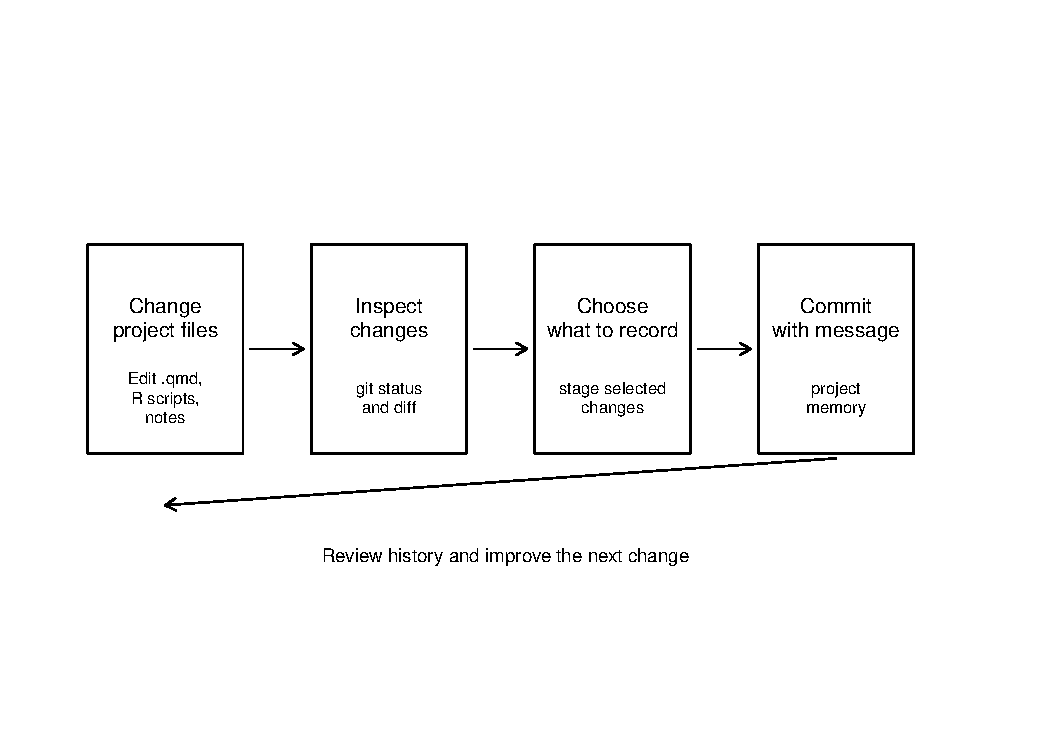
\includegraphics[width=0.9\linewidth,height=\textheight,keepaspectratio,alt={A left-to-right workflow diagram showing project changes moving through inspect, choose, commit, and review steps.}]{chapters/21-collaboration-and-version-control_files/figure-pdf/fig-21-version-control-flow-1.pdf}

}

\caption{\label{fig-21-version-control-flow}A Simple Version-Control
Flow for Analytical Project Work.}

\end{figure}%

The key point in Figure~\ref{fig-21-version-control-flow} is that
version control is not just the commit. The commit is one moment in a
larger habit. Leo must first inspect what changed. Then he must choose
what belongs together. Then he records the change. Later, the history
becomes a resource for review, recovery, collaboration, and explanation.

The smallest useful question before each commit is:

\begin{quote}
Do these changes belong together?
\end{quote}

If Leo corrected a typo in the chapter and also rewrote the
data-cleaning script, those may be two different commits. If he updated
a source note and the corresponding import script together, those may
belong in one commit. The point is not perfection. The point is readable
history.

\section{Collaboration Without Chaos}\label{collaboration-without-chaos}

Version control becomes even more valuable when more than one person
works on the project.

Collaboration without version control often becomes an exchange of
attachments:

\begin{itemize}
\tightlist
\item
  ``Please use the latest file.''
\item
  ``I think I edited the old one.''
\item
  ``Can you merge my comments?''
\item
  ``Which report has the corrected table?''
\item
  ``Who changed the filtering rule?''
\item
  ``Why is my version different from yours?''
\end{itemize}

Git-based collaboration introduces a more structured vocabulary.

A \textbf{branch} is a parallel line of work. It lets a person make
changes without immediately disturbing the main version of the project.

A \textbf{pull request} is a proposed change submitted for review before
it enters the shared main version. The name may sound technical, but the
idea is familiar: ``Here is my proposed improvement. Please inspect it
before we adopt it.''

An \textbf{issue} is a structured note about something that needs
attention: a bug, a missing task, a requested improvement, a discussion
point, or a decision that should not disappear into private memory.

A \textbf{review} is the act of checking proposed changes before they
become part of the shared project.

Leo does not need to master every collaboration feature at once. He
needs the professional idea:

\begin{quote}
Collaboration improves when changes are proposed, discussed, reviewed,
and recorded instead of silently overwritten.
\end{quote}

This is especially important for analytical projects. A small code
change may alter a table. A changed filter may alter a claim. A revised
figure may alter an interpretation. Version control gives collaborators
a place to discuss the change before it enters the shared work.

\begin{tcolorbox}[enhanced jigsaw, arc=.35mm, bottomrule=.15mm, breakable, colback=white, colframe=quarto-callout-note-color-frame, left=2mm, leftrule=.75mm, opacityback=0, rightrule=.15mm, toprule=.15mm]
\begin{minipage}[t]{5.5mm}
\textcolor{quarto-callout-note-color}{\faInfo}
\end{minipage}%
\begin{minipage}[t]{\textwidth - 5.5mm}

\vspace{-3mm}\textbf{Collaboration is not just access}\vspace{3mm}

Giving collaborators access to files is not the same as coordinating
analytical change. Collaboration needs shared structure, visible
history, and reviewable decisions.

\end{minipage}%
\end{tcolorbox}

This is why GitHub can be useful beyond storage. It gives a team a place
to combine version history with issues, review, discussion, and remote
coordination. But the beginner lesson remains grounded: no platform can
replace disciplined project habits.

\section{What Version Control Does Not
Solve}\label{what-version-control-does-not-solve}

Version control is powerful, but it is not magic.

It does not make bad analysis good. It does not explain an undocumented
decision unless someone writes the explanation. It does not protect
secrets if Leo commits them. It does not make a huge dataset easy to
share if Git is the wrong storage tool. It does not make an unstable
live connection reproducible unless the workflow controls the evidence.

Git records history. It does not judge whether the history is wise.

That distinction matters because beginners sometimes expect tools to
replace judgment. A reproducible Quarto report still needs good code. A
connected data workflow still needs source notes. A version-controlled
repository still needs meaningful commits, safe file choices, and
careful collaboration.

\begin{tcolorbox}[enhanced jigsaw, arc=.35mm, bottomrule=.15mm, breakable, colback=white, colframe=quarto-callout-warning-color-frame, left=2mm, leftrule=.75mm, opacityback=0, rightrule=.15mm, toprule=.15mm]
\begin{minipage}[t]{5.5mm}
\textcolor{quarto-callout-warning-color}{\faExclamationTriangle}
\end{minipage}%
\begin{minipage}[t]{\textwidth - 5.5mm}

\vspace{-3mm}\textbf{Git records mistakes too}\vspace{3mm}

Version control can help Leo recover from mistakes, but it can also
preserve mistakes in the project history. This is why he should inspect
changes before committing and avoid tracking files that should remain
private.

\end{minipage}%
\end{tcolorbox}

The safest mental model is this:

\begin{itemize}
\tightlist
\item
  Quarto helps connect code, output, and explanation.
\item
  Chapter 20's data discipline helps control evidence entering the
  project.
\item
  Version control helps record how the project changes after that.
\item
  Collaboration tools help people review and coordinate those changes.
\end{itemize}

Each layer supports the others. None replaces the others.

\section{Common Beginner Mistakes}\label{common-beginner-mistakes-12}

The mistakes in this chapter are often quiet. They do not always break
the project immediately. They make future work harder.

One common mistake is treating Git as a backup system only. Backup
matters, but version control is not merely a spare copy. Its value is in
readable history.

Another mistake is committing everything. Beginners may track caches,
rendered books, large outputs, workspace files, private notes,
credentials, and raw data without checking whether those files belong in
permanent history.

A third mistake is writing commit messages that say nothing. A history
full of \texttt{update}, \texttt{fix}, and \texttt{final} does not help
future Leo understand decisions.

A fourth mistake is committing too rarely. If Leo works for three weeks
and creates one huge commit, the history becomes difficult to inspect.
Meaningful smaller commits are easier to review and recover.

A fifth mistake is mixing unrelated work in one commit. A correction to
the import script, a rewrite of the introduction, and a change to a plot
label may not belong together.

A sixth mistake is assuming GitHub and Git are the same. GitHub hosts
and supports collaboration, but the tracking logic comes from Git.

A seventh mistake is versioning secrets. This is serious because Git
history can preserve what the current file no longer shows.

An eighth mistake is using branches, pull requests, or issues as
decorative terms without understanding their role. Their purpose is to
make change visible, discussable, and reviewable.

\begin{tcolorbox}[enhanced jigsaw, arc=.35mm, bottomrule=.15mm, breakable, colback=white, colframe=quarto-callout-tip-color-frame, left=2mm, leftrule=.75mm, opacityback=0, rightrule=.15mm, toprule=.15mm]
\begin{minipage}[t]{5.5mm}
\textcolor{quarto-callout-tip-color}{\faLightbulb}
\end{minipage}%
\begin{minipage}[t]{\textwidth - 5.5mm}

\vspace{-3mm}\textbf{The beginner's control question}\vspace{3mm}

Before recording a change, Leo can ask: ``Would this commit help someone
understand what changed, why it changed, and how to recover the earlier
state if necessary?''

\end{minipage}%
\end{tcolorbox}

That question is enough to improve most beginner version-control habits.

\section{Try It Yourself}\label{try-it-yourself-7}

Open a project folder from previous analytical work, but do not change
anything yet.

First, inspect the file names. Look for signs of hidden history:

\begin{itemize}
\tightlist
\item
  \texttt{final};
\item
  \texttt{new};
\item
  \texttt{old};
\item
  \texttt{updated};
\item
  \texttt{copy};
\item
  repeated dates;
\item
  initials from collaborators;
\item
  scripts with numbered suffixes;
\item
  reports with contradictory names.
\end{itemize}

Then answer these questions in a notebook:

\begin{enumerate}
\def\labelenumi{\arabic{enumi}.}
\tightlist
\item
  Which files appear to be versions of the same work?
\item
  Can you tell which version is authoritative?
\item
  Can you tell what changed between versions?
\item
  Can you tell why the change was made?
\item
  Could someone else reconstruct the history without asking you?
\item
  Which files would belong in version control?
\item
  Which files should be ignored, archived elsewhere, or kept private?
\end{enumerate}

The purpose is not to shame old habits. Those habits were survival
strategies. The purpose is to see why professional project history
requires more than file names.

Now imagine the same project under version control. What commit messages
would have helped?

Write three possible commit messages for past changes you can infer from
the folder.

For example:

\begin{Shaded}
\begin{Highlighting}[]
\NormalTok{Add first cleaned version of learner dataset}
\NormalTok{Revise report after correcting missing project scores}
\NormalTok{Update figure labels for Chapter 18 communication section}
\end{Highlighting}
\end{Shaded}

If the message would have helped future you understand the project, it
is already teaching the right habit.

\section{A Small Practice Lab}\label{a-small-practice-lab-8}

In this lab, Leo does not need to create a public repository or connect
to GitHub. The focus is conceptual control.

Start with a small local R or Quarto project. It can be a practice copy,
not the only copy of important work.

\begin{enumerate}
\def\labelenumi{\arabic{enumi}.}
\tightlist
\item
  Identify the project root. Confirm where \texttt{\_quarto.yml},
  \texttt{.Rproj}, or the main scripts live.
\item
  List the files that explain the project: \texttt{.qmd}, \texttt{.R},
  \texttt{README}, source notes, configuration files, and approved small
  data files.
\item
  List files that should not enter version history: credentials, private
  data, caches, huge generated outputs, and machine-specific clutter.
\item
  Draft a \texttt{.gitignore} pattern before tracking files.
\item
  Make one small project improvement, such as correcting a paragraph,
  improving a comment, or updating a source note.
\item
  Inspect what changed. At minimum, Leo should know which files changed
  and what changed inside them before recording anything.
\item
  Decide whether the change deserves its own commit.
\item
  Write a commit message that explains the change.
\item
  Repeat the exercise with a second, unrelated change and write a
  separate message.
\end{enumerate}

The lab has one central rule:

\begin{quote}
Do not record changes you have not inspected.
\end{quote}

This rule protects Leo from accidental commits. It also slows the
workflow just enough to make the history meaningful.

If Leo is working with collaborators, add three more questions:

\begin{enumerate}
\def\labelenumi{\arabic{enumi}.}
\tightlist
\item
  Should this change be discussed before it enters the main version?
\item
  Would an issue help record the problem or task?
\item
  Would a branch or pull request make review safer?
\end{enumerate}

Those questions are not bureaucracy. They are collaboration safety.

\section{Short Recap}\label{short-recap-7}

A project folder can store files without remembering decisions. Version
control solves that problem by recording meaningful changes over time.

Git is a local system for tracking project history. GitHub is a remote
collaboration platform that can host Git repositories and support shared
work. They are related, but they are not the same.

A commit is a meaningful snapshot of project change, ideally recorded
with a message that explains why the change matters.

Version control works best when the project is already structured. The
official \texttt{data/} route still matters. Source notes still matter.
Quarto reports still matter. Version control records how these pieces
change.

Not everything belongs in Git. Quarto source files, R scripts,
documentation, source notes, small configuration files, and approved
teaching data may belong. Credentials, secrets, huge files, private
data, temporary outputs, and machine-specific clutter usually do not.

\texttt{.gitignore} helps prevent unwanted files from entering the
repository, but it works best before those files are committed.

Collaboration becomes safer when changes are visible, proposed,
reviewed, and discussed rather than silently overwritten.

\section{Leo's Notebook}\label{leos-notebook-10}

Leo writes:

\begin{quote}
My old folders kept copies. They did not keep history.
\end{quote}

He underlines the distinction.

A copy can preserve a file, but it cannot explain why the file changed.
A synced folder can move changes between machines, but it cannot
guarantee that the change was inspected. A backup can rescue files after
a failure, but it does not automatically create a readable decision
record.

Version control gives the project memory.

Leo also writes a warning to himself:

\begin{quote}
Git remembers. Do not give it secrets.
\end{quote}

That sentence changes how he thinks about credentials, private data, and
large files. In Chapter 20, he learned that connected data needs
controlled access. In Chapter 21, he learns that project history also
needs controlled boundaries.

His final note is practical:

\begin{quote}
A good commit should help future me understand the work faster.
\end{quote}

That is the habit he will carry forward.

\section{Glossary}\label{glossary-7}

\textbf{Backup}\\
A spare copy of files kept to reduce loss if a machine, drive, or
storage location fails. A backup is useful, but it is not the same as a
structured history of project changes.

\textbf{Branch}\\
A parallel line of work in a Git repository. Branches allow changes to
be developed without immediately altering the main version of the
project.

\textbf{Commit}\\
A recorded snapshot of selected project changes, usually accompanied by
a message explaining the purpose of the change.

\textbf{Commit message}\\
A short explanation attached to a commit. A useful commit message helps
future readers understand why the change was made.

\textbf{Git}\\
A version control system that tracks the history of files in a project
repository.

\textbf{GitHub}\\
A remote hosting and collaboration platform for Git repositories. It
supports shared access, issues, pull requests, review, and other
collaboration features.

\textbf{Issue}\\
A structured note in a collaboration platform, often used to record a
bug, task, question, proposed improvement, or discussion point.

\textbf{Pull request}\\
A proposed change submitted for review before it is merged into a shared
version of a repository.

\textbf{Repository}\\
A project folder that has a version-control history attached to it.

\textbf{Review}\\
The process of inspecting proposed changes before accepting them into
the shared project.

\textbf{Staging}\\
The act of selecting which changes should be included in the next
commit.

\textbf{Syncing}\\
Keeping files updated across devices or cloud locations. Syncing can
support access, but it is not the same as version control.

\textbf{Version control}\\
A system for recording, inspecting, and recovering the history of
meaningful changes in a project.

\textbf{\texttt{.gitignore}}\strut \\
A file that tells Git which files or patterns should usually be ignored.

\section{Chapter Outcome}\label{chapter-outcome-20}

Leo can now explain why professional analytical projects need a
traceable history. He can distinguish saving, backing up, syncing, and
version control. He can explain Git as a local tracking system and
GitHub as a remote collaboration space, without confusing the two.

He understands commits as meaningful snapshots, not random saves. He can
describe why commit messages matter, why \texttt{.gitignore} protects a
project, and why secrets, credentials, huge files, temporary outputs,
private data, and machine-specific clutter should not enter version
history.

He can also explain how version control fits the R and Quarto workflow.
The official \texttt{data/} route remains the route for evidence.
Scripts, Quarto chapters, documentation, and source notes help explain
the work. Version control records how those pieces change over time.

Most importantly, Leo now sees collaboration as more than shared access.
Serious collaboration requires visible changes, reviewable decisions,
and a project memory strong enough to survive correction.

\section{What Comes Next}\label{what-comes-next-9}

Leo now has a project that can remember.

Chapter 19 helped him turn analysis into a reproducible report. Chapter
20 helped him control evidence that enters from beyond local files.
Chapter 21 has now helped him make project change traceable,
recoverable, and safer to share.

The next problem is not history.

It is reuse.

As Leo's work improves, he begins to notice repeated actions across
scripts and reports. He cleans text fields again. He standardises
yes-or-no values again. He creates score bands again. He writes small
helper functions, then copies them from one script into another. At
first, that feels efficient. Soon, it creates a new form of disorder:
useful functions scattered across files, projects, and versions.

Chapter 22 takes the next professional step.

It asks what happens when reusable functions need an organised home, and
why a traceable project history makes that organisation safer to build,
revise, test, and share.

That is where Leo moves from functions to packages.

\chapter{From Functions to Packages: Building Reusable R
Tools}\label{from-functions-to-packages-building-reusable-r-tools}

\renewcommand{\thefigure}{22.\arabic{figure}}  

\setcounter{figure}{0}

\renewcommand{\thetable}{22.\arabic{table}}  

\setcounter{table}{0}

\section{Opening Scene: When Useful Functions Become Hard to
Control}\label{opening-scene-when-useful-functions-become-hard-to-control}

Leo now has a project that can remember.

In
\hyperref[collaboration-and-version-control-making-work-traceable]{Chapter
21}, he learned that serious analytical work needs traceable history. A
project should not depend on folders called \texttt{final},
\texttt{final\_2}, and \texttt{real\_final}. It should record meaningful
changes, protect sensitive files, and make collaboration easier to
inspect.

That solved one professional problem.

Then another problem appears.

Inside Leo's scripts, useful functions are beginning to multiply:

\begin{Shaded}
\begin{Highlighting}[]
\NormalTok{clean\_text\_field }\OtherTok{\textless{}{-}} \ControlFlowTok{function}\NormalTok{(x) \{}
  \FunctionTok{trimws}\NormalTok{(}\FunctionTok{tolower}\NormalTok{(}\FunctionTok{gsub}\NormalTok{(}\StringTok{"}\SpecialCharTok{\textbackslash{}\textbackslash{}}\StringTok{s+"}\NormalTok{, }\StringTok{" "}\NormalTok{, }\FunctionTok{as.character}\NormalTok{(x))))}
\NormalTok{\}}

\NormalTok{standardise\_yes\_no }\OtherTok{\textless{}{-}} \ControlFlowTok{function}\NormalTok{(x) \{}
\NormalTok{  value }\OtherTok{\textless{}{-}} \FunctionTok{clean\_text\_field}\NormalTok{(x)}

\NormalTok{  out }\OtherTok{\textless{}{-}} \FunctionTok{rep}\NormalTok{(}\ConstantTok{NA}\NormalTok{, }\FunctionTok{length}\NormalTok{(value))}
\NormalTok{  out[value }\SpecialCharTok{\%in\%} \FunctionTok{c}\NormalTok{(}\StringTok{"yes"}\NormalTok{, }\StringTok{"y"}\NormalTok{, }\StringTok{"true"}\NormalTok{, }\StringTok{"1"}\NormalTok{)] }\OtherTok{\textless{}{-}} \ConstantTok{TRUE}
\NormalTok{  out[value }\SpecialCharTok{\%in\%} \FunctionTok{c}\NormalTok{(}\StringTok{"no"}\NormalTok{, }\StringTok{"n"}\NormalTok{, }\StringTok{"false"}\NormalTok{, }\StringTok{"0"}\NormalTok{)] }\OtherTok{\textless{}{-}} \ConstantTok{FALSE}

\NormalTok{  out}
\NormalTok{\}}

\NormalTok{make\_score\_band }\OtherTok{\textless{}{-}} \ControlFlowTok{function}\NormalTok{(score) \{}
  \FunctionTok{ifelse}\NormalTok{(}
    \FunctionTok{is.na}\NormalTok{(score), }\ConstantTok{NA\_character\_}\NormalTok{,}
    \FunctionTok{ifelse}\NormalTok{(score }\SpecialCharTok{\textgreater{}=} \DecValTok{80}\NormalTok{, }\StringTok{"high"}\NormalTok{,}
           \FunctionTok{ifelse}\NormalTok{(score }\SpecialCharTok{\textgreater{}=} \DecValTok{60}\NormalTok{, }\StringTok{"moderate"}\NormalTok{, }\StringTok{"developing"}\NormalTok{))}
\NormalTok{  )}
\NormalTok{\}}
\end{Highlighting}
\end{Shaded}

At first, this feels like progress. Leo is no longer rewriting every
cleaning rule from scratch. He can name a rule once and call it again.

But the functions do not stay neatly in one place. One copy lives in a
cleaning script. Another copy appears in a Quarto report. A third copy
gets pasted into a collaborator's project. Then Leo improves one version
of \texttt{clean\_text\_field()} but forgets that two older versions
still exist elsewhere.

The functions are useful.

That is exactly why the disorder matters.

A project with traceable history can show Leo what changed. It cannot,
by itself, solve the problem of reusable functions scattered across
scripts. Traceability protects the record of change. Reuse needs a
stable home.

This chapter begins there.

\begin{tcolorbox}[enhanced jigsaw, arc=.35mm, bottomrule=.15mm, breakable, colback=white, colframe=quarto-callout-important-color-frame, left=2mm, leftrule=.75mm, opacityback=0, rightrule=.15mm, toprule=.15mm]
\begin{minipage}[t]{5.5mm}
\textcolor{quarto-callout-important-color}{\faExclamation}
\end{minipage}%
\begin{minipage}[t]{\textwidth - 5.5mm}

\vspace{-3mm}\textbf{The lightbulb idea}\vspace{3mm}

A function names one reusable action. A package organises related
reusable actions into a tool that can be loaded, documented, tested,
shared, and trusted.

\end{minipage}%
\end{tcolorbox}

This chapter does not turn Leo into a professional package maintainer.
It does not teach CRAN submission, release engineering, continuous
integration, or advanced object systems.

It teaches a simpler and more important idea:

\begin{quote}
A package is not only something Leo installs. It can also be a
disciplined way to organise his own reusable R work.
\end{quote}

\section{What Changes After Chapter
21}\label{what-changes-after-chapter-21}

Chapter 21 taught Leo to protect the history of a project. That matters
before a project grows further because reusable tools become risky when
their changes cannot be traced.

If Leo puts related functions into a shared toolkit, those functions
will evolve. He may correct an assumption in
\texttt{standardise\_yes\_no()}. He may change the threshold used by
\texttt{make\_score\_band()}. He may add a new helper for dates, missing
values, or learner-status categories.

When those changes affect several analyses, Leo needs two kinds of
control:

\begin{itemize}
\tightlist
\item
  version control, so he can inspect how the tool changed;
\item
  tool organisation, so the reusable logic lives in one deliberate
  place.
\end{itemize}

Chapter 22 builds on Chapter 21 by asking a new question:

\begin{quote}
Once a project can remember its history, where should reusable
analytical tools live?
\end{quote}

The answer is not always ``make a package.'' Sometimes a function should
remain inside a script. Sometimes a small helper file is enough.
Sometimes a project-level toolkit is the right middle ground. But when
related functions are reused across scripts, reports, projects, or
collaborators, Leo has reached the package question.

The movement in this chapter is shown in
Figure~\ref{fig-22-function-to-package-flow}.

\begin{figure}

\centering{

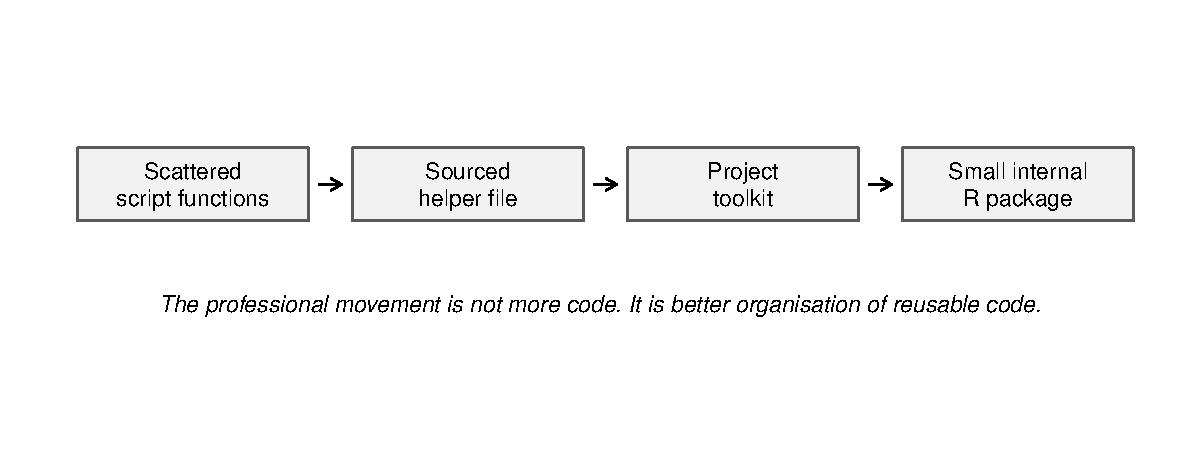
\includegraphics[width=0.9\linewidth,height=\textheight,keepaspectratio,alt={A left-to-right diagram showing scattered script functions becoming a sourced helper file, then a project toolkit, and finally a small internal R package.}]{chapters/22-from-functions-to-packages_files/figure-pdf/fig-22-function-to-package-flow-1.pdf}

}

\caption{\label{fig-22-function-to-package-flow}From Scattered Helper
Functions to a Reusable R Toolkit.}

\end{figure}%

Figure~\ref{fig-22-function-to-package-flow} is deliberately modest. It
does not say that every learner must create a package immediately. It
says that reusable work has stages. Leo needs to recognise which stage
his project has reached.

\section{Revisiting the Function Story Without Repeating
It}\label{revisiting-the-function-story-without-repeating-it}

\hyperref[built-in-functions-rs-ready-made-action-system]{Chapter 8}
introduced built-in functions as R's ready-made action system. Leo
learned that functions such as \texttt{mean()}, \texttt{summary()},
\texttt{length()}, \texttt{tolower()}, and \texttt{trimws()} are named
actions R already knows how to perform. That chapter focused on using
existing tools well.

\hyperref[user-defined-functions-naming-actions-of-your-own]{Chapter 9}
moved one step further. Leo learned to create small user-defined
functions when the same idea appeared repeatedly. Instead of writing the
same text-cleaning rule across several lines, he could name the rule and
call it deliberately.

Chapter 22 is not a repeat of those lessons. It asks what happens after
Leo has several useful functions of his own.

A single user-defined function solves a local repetition problem. A
group of related user-defined functions creates an organisation problem.

For example, suppose Leo repeatedly uses these helpers in his
\texttt{df\_r\_migration} workflow:

\begin{Shaded}
\begin{Highlighting}[]
\FunctionTok{clean\_text\_field}\NormalTok{(}\FunctionTok{c}\NormalTok{(}\StringTok{" Nigeria "}\NormalTok{, }\StringTok{"SOUTH  AFRICA"}\NormalTok{, }\StringTok{"ghana"}\NormalTok{))}
\CommentTok{\#\textgreater{} [1] "nigeria"      "south africa" "ghana"}

\FunctionTok{make\_score\_band}\NormalTok{(}\FunctionTok{c}\NormalTok{(}\DecValTok{92}\NormalTok{, }\DecValTok{74}\NormalTok{, }\DecValTok{51}\NormalTok{, }\ConstantTok{NA}\NormalTok{))}
\CommentTok{\#\textgreater{} [1] "high"       "moderate"   "developing" NA}

\FunctionTok{standardise\_yes\_no}\NormalTok{(}\FunctionTok{c}\NormalTok{(}\StringTok{"Yes"}\NormalTok{, }\StringTok{"N"}\NormalTok{, }\StringTok{"TRUE"}\NormalTok{, }\StringTok{"0"}\NormalTok{, }\StringTok{"not available"}\NormalTok{))}
\CommentTok{\#\textgreater{} [1]  TRUE FALSE  TRUE FALSE    NA}
\end{Highlighting}
\end{Shaded}

Each function is small. Each one is understandable. But together they
now form a toolkit for preparing learner data.

That is a new threshold.

Leo is no longer only writing functions. He is beginning to build tools.

\section{Why Copying Functions Is Not a
Workflow}\label{why-copying-functions-is-not-a-workflow}

Copying a function from one script into another feels efficient because
it produces immediate progress. The code is already there. The output
works. The report renders.

The danger appears later.

Suppose Leo has three scripts:

\begin{Shaded}
\begin{Highlighting}[]
\NormalTok{scripts/12{-}clean{-}data.R}
\NormalTok{scripts/15{-}summarise{-}learners.R}
\NormalTok{chapters/19{-}reproducible{-}reports{-}with{-}quarto.qmd}
\end{Highlighting}
\end{Shaded}

Each file contains its own copy of \texttt{clean\_text\_field()}.

Then Leo notices a problem. The function handles extra spaces, but it
does not handle missing values carefully enough. He fixes the version in
\texttt{scripts/12-clean-data.R}.

But the old version remains in the other two files.

Now the project contains one function name with several behaviours. The
danger is not that R refuses to run. The danger is that the project may
run with different assumptions in different places.

\begin{tcolorbox}[enhanced jigsaw, arc=.35mm, bottomrule=.15mm, breakable, colback=white, colframe=quarto-callout-warning-color-frame, left=2mm, leftrule=.75mm, opacityback=0, rightrule=.15mm, toprule=.15mm]
\begin{minipage}[t]{5.5mm}
\textcolor{quarto-callout-warning-color}{\faExclamationTriangle}
\end{minipage}%
\begin{minipage}[t]{\textwidth - 5.5mm}

\vspace{-3mm}\textbf{Copying is not reuse}\vspace{3mm}

Copying a helper function creates more locations to maintain. Reuse
means keeping the rule in one controlled place and calling it when
needed.

\end{minipage}%
\end{tcolorbox}

This distinction is central to professional R work. A repeated function
should not become a hidden family of slightly different copies. It
should become a shared tool with one source of truth.

\section{From a Loose Function to a Small
Toolkit}\label{from-a-loose-function-to-a-small-toolkit}

Leo does not need to jump from one helper function straight into a
formal package. There are stages between chaos and package development.
Table~\ref{tbl-22-reuse-stages} gives him a practical map.

{

\begin{longtable}[]{@{}
  >{\raggedright\arraybackslash}p{(\linewidth - 8\tabcolsep) * \real{0.0826}}
  >{\raggedright\arraybackslash}p{(\linewidth - 8\tabcolsep) * \real{0.2752}}
  >{\raggedright\arraybackslash}p{(\linewidth - 8\tabcolsep) * \real{0.2110}}
  >{\raggedright\arraybackslash}p{(\linewidth - 8\tabcolsep) * \real{0.2385}}
  >{\raggedright\arraybackslash}p{(\linewidth - 8\tabcolsep) * \real{0.1927}}@{}}

\caption{\label{tbl-22-reuse-stages}Five Stages of Organising Reusable R
Functions.}

\tabularnewline

\toprule\noalign{}
\begin{minipage}[b]{\linewidth}\raggedright
Stage
\end{minipage} & \begin{minipage}[b]{\linewidth}\raggedright
Best used when
\end{minipage} & \begin{minipage}[b]{\linewidth}\raggedright
Strength
\end{minipage} & \begin{minipage}[b]{\linewidth}\raggedright
Risk
\end{minipage} & \begin{minipage}[b]{\linewidth}\raggedright
Control question
\end{minipage} \\
\midrule\noalign{}
\endhead
\bottomrule\noalign{}
\endlastfoot
Loose function in a script & The function serves one analysis and is
unlikely to be reused elsewhere. & Fast and local. & Easy to copy,
forget, or change inconsistently. & Is this function only needed
here? \\
Sourced helper file & Several scripts in one project need the same
helper functions. & Keeps shared helpers in one file. & Can become
crowded as the project grows. & Do several files need the same
helper? \\
Project toolkit & A project has a small set of stable helpers used
across reports and scripts. & Makes project-specific tools easier to
find and maintain. & May lack formal documentation or testing if not
managed deliberately. & Are these helpers part of this project's regular
workflow? \\
Small internal package & Related functions need structure,
documentation, tests, and controlled loading. & Gives reusable functions
a formal home with documentation and tests. & Can be overbuilt if the
functions are not yet stable or reused. & Do these related functions
need a stable documented structure? \\
Public CRAN-style package & The tool is intended for broad external use
and must satisfy public release expectations. & Supports wider
distribution and stronger user-facing discipline. & Requires much more
maintenance, checking, policy awareness, and user support. & Is this
tool ready for users beyond the project team? \\

\end{longtable}

}

Table~\ref{tbl-22-reuse-stages} prevents two opposite mistakes. The
first mistake is staying too informal for too long, until helper
functions are scattered across files. The second mistake is turning
every small function into a package before the need is real.

The professional habit is judgment.

Leo should ask what kind of reuse he is dealing with. A one-off helper
can stay in a script. A few shared helpers can live in a sourced file. A
stable family of functions may deserve a package structure.

A sourced helper file is often the first serious improvement because it
gives the project one place to load shared functions instead of copying
them into several scripts. Listing~\ref{lst-22-source-helper-file} shows
the idea without turning it into a full package.

\begin{codelisting}

\caption{\label{lst-22-source-helper-file}Loading a Shared Helper File
Without Copying Functions.}

\centering{

\begin{Shaded}
\begin{Highlighting}[]
\FunctionTok{source}\NormalTok{(}\StringTok{"scripts/helpers.R"}\NormalTok{)}

\NormalTok{df\_r\_migration}\SpecialCharTok{$}\NormalTok{country }\OtherTok{\textless{}{-}} \FunctionTok{clean\_text\_field}\NormalTok{(df\_r\_migration}\SpecialCharTok{$}\NormalTok{country)}
\NormalTok{df\_r\_migration}\SpecialCharTok{$}\NormalTok{used\_quarto }\OtherTok{\textless{}{-}} \FunctionTok{standardise\_yes\_no}\NormalTok{(df\_r\_migration}\SpecialCharTok{$}\NormalTok{used\_quarto)}
\end{Highlighting}
\end{Shaded}

}

\end{codelisting}%

Listing~\ref{lst-22-source-helper-file} is useful because the function
definitions now live in one shared helper file. In this example,
\texttt{scripts/helpers.R} is an ordinary project helper file, not the
special \texttt{R/} folder used inside an R package. That distinction
matters because a helper file can reduce copying, but it is still not a
package. It has no package identity, no formal export rules, no help
pages, and no built-in testing structure. That limitation explains why a
stable family of functions may eventually need a stronger home.

\section{What a Package Really Is}\label{what-a-package-really-is}

Earlier chapters introduced packages mostly from the user's side. Leo
installed packages, loaded them, and used functions written by other
people. That user-side view is still correct, but it is not complete.

From the author's side, an R package is an organised project structure
for related R functions and their supporting materials. It is not the
analysis itself, not the raw data, and not the final report. It is the
reusable tool layer that helps those parts of the workflow behave
consistently.

At beginner level, Leo can think of a package as a folder with rules:

\begin{itemize}
\tightlist
\item
  the functions live in predictable places;
\item
  the package describes itself;
\item
  the package declares what it makes available;
\item
  the package can include documentation;
\item
  the package can include examples;
\item
  the package can include tests;
\item
  the package can be loaded as a tool rather than copied as loose code.
\end{itemize}

This definition matters because it removes a false barrier. A package
does not have to be famous. It does not have to be on CRAN. It does not
have to solve a global problem.

A package can begin as an internal tool that helps Leo and his
collaborators keep repeated analytical logic organised.

\begin{tcolorbox}[enhanced jigsaw, arc=.35mm, bottomrule=.15mm, breakable, colback=white, colframe=quarto-callout-note-color-frame, left=2mm, leftrule=.75mm, opacityback=0, rightrule=.15mm, toprule=.15mm]
\begin{minipage}[t]{5.5mm}
\textcolor{quarto-callout-note-color}{\faInfo}
\end{minipage}%
\begin{minipage}[t]{\textwidth - 5.5mm}

\vspace{-3mm}\textbf{Package as structure, not status}\vspace{3mm}

A package is not automatically a public product. It can be a disciplined
structure for organising reusable R functions inside a project, research
group, classroom, or team.

\end{minipage}%
\end{tcolorbox}

That is the Chapter 22 shift. Leo is no longer only a package user. He
is beginning to understand package thinking from the author side.

\section{The Smallest Useful Package Mental
Model}\label{the-smallest-useful-package-mental-model}

The smallest useful package does not need to be impressive. It needs to
be coherent.

For this book, imagine a teaching package called \texttt{rwaytools}. The
name is only an example. It is not a real package claim and it is not
being prepared for CRAN in this chapter.

The package might contain functions such as:

\begin{itemize}
\tightlist
\item
  \texttt{clean\_text\_field()}, for standardising text fields such as
  \texttt{country}, \texttt{industry}, \texttt{background}, and
  \texttt{completion\_status};
\item
  \texttt{standardise\_yes\_no()}, for converting mixed yes-or-no values
  into logical values;
\item
  \texttt{make\_score\_band()}, for turning assessment scores into
  labelled bands;
\item
  \texttt{check\_required\_columns()}, for checking whether a dataset
  has the columns a workflow expects.
\end{itemize}

These functions belong together because they support one kind of work:
preparing and checking learner data before analysis.

The package idea does not make the functions more complicated. It makes
their home more reliable.

The beginner-friendly skeleton in Listing~\ref{lst-22-package-skeleton}
shows the structure Leo should recognise before he tries to build
anything advanced.

\begin{codelisting}

\caption{\label{lst-22-package-skeleton}A Beginner-Friendly Skeleton of
a Small Internal R Package.}

\centering{

\begin{Shaded}
\begin{Highlighting}[]
\NormalTok{rwaytools/}
\NormalTok{├── DESCRIPTION}
\NormalTok{├── LICENSE}
\NormalTok{├── NAMESPACE}
\NormalTok{├── R/}
\NormalTok{│   ├── clean{-}text{-}field.R}
\NormalTok{│   ├── standardise{-}yes{-}no.R}
\NormalTok{│   └── make{-}score{-}band.R}
\NormalTok{├── man/}
\NormalTok{│   ├── clean\_text\_field.Rd}
\NormalTok{│   ├── standardise\_yes\_no.Rd}
\NormalTok{│   └── make\_score\_band.Rd}
\NormalTok{└── tests/}
\NormalTok{    └── testthat/}
\NormalTok{        ├── test{-}clean{-}text{-}field.R}
\NormalTok{        ├── test{-}standardise{-}yes{-}no.R}
\NormalTok{        └── test{-}make{-}score{-}band.R}
\end{Highlighting}
\end{Shaded}

}

\end{codelisting}%

Listing~\ref{lst-22-package-skeleton} is not a command to run. It is a
map. The map tells Leo that a package is not one giant script. It is a
structured home for related functions, identity information,
documentation, and checks.

\section{Anatomy of a Beginner-Friendly R
Package}\label{anatomy-of-a-beginner-friendly-r-package}

The package skeleton becomes easier to understand when each part has a
job. Table~\ref{tbl-22-package-anatomy} gives Leo the first practical
map.

{

\begin{longtable}[]{@{}
  >{\raggedright\arraybackslash}p{(\linewidth - 6\tabcolsep) * \real{0.0793}}
  >{\raggedright\arraybackslash}p{(\linewidth - 6\tabcolsep) * \real{0.5683}}
  >{\raggedright\arraybackslash}p{(\linewidth - 6\tabcolsep) * \real{0.1278}}
  >{\raggedright\arraybackslash}p{(\linewidth - 6\tabcolsep) * \real{0.2247}}@{}}

\caption{\label{tbl-22-package-anatomy}Core Parts of a Beginner-Friendly
R Package.}

\tabularnewline

\toprule\noalign{}
\begin{minipage}[b]{\linewidth}\raggedright
Part
\end{minipage} & \begin{minipage}[b]{\linewidth}\raggedright
Main job
\end{minipage} & \begin{minipage}[b]{\linewidth}\raggedright
Beginner interpretation
\end{minipage} & \begin{minipage}[b]{\linewidth}\raggedright
Needed immediately?
\end{minipage} \\
\midrule\noalign{}
\endhead
\bottomrule\noalign{}
\endlastfoot
\texttt{R/} & Stores the R function files that define the package's
reusable actions. & Where Leo's functions live. & Yes, for any package
with functions. \\
\texttt{DESCRIPTION} & Identifies the package and records basic metadata
such as name, version, title, description, authors, licence, and
dependencies. & The package identity card. & Yes. \\
\texttt{NAMESPACE} & Controls which functions are exported for users and
which external functions are imported for package use. & The package
access map. & Yes, though beginners often let tools generate it. \\
\texttt{man/} & Stores help files generated from documentation comments
or written manually. & The help system. & Usually, once functions are
meant to be reused. \\
\texttt{tests/testthat/} & Stores tests that check whether important
functions behave as expected. & The trust-checking area. & Recommended
for important reusable functions. \\
\texttt{README} & Introduces the package to human readers and shows
common use cases. & The front door for readers. & Useful, especially for
collaborators. \\
\texttt{vignettes/} & Stores longer tutorials or worked examples when
the package needs extended guidance. & The extended teaching space. &
Optional for beginners. \\

\end{longtable}

}

Table~\ref{tbl-22-package-anatomy} should not be memorised as a
checklist for publication. It is a mental map. The essential point is
that a package gives reusable work a recognisable architecture.

That architecture gives future Leo two advantages. First, he knows where
to look. Second, he knows what kind of support each function needs
before other people depend on it.

\section{\texorpdfstring{The \texttt{R/} Folder: Where Functions
Live}{The R/ Folder: Where Functions Live}}\label{the-r-folder-where-functions-live}

The \texttt{R/} folder is the simplest part of the package to
understand. It contains R scripts that define functions.

A beginner mistake is to imagine that one package must have one giant R
file. That is not the point. The \texttt{R/} folder can contain several
files, and each file can hold one function or a small group of closely
related functions.

For Leo's teaching package, the \texttt{R/} folder might contain:

\begin{Shaded}
\begin{Highlighting}[]
\NormalTok{R/clean{-}text{-}field.R}
\NormalTok{R/standardise{-}yes{-}no.R}
\NormalTok{R/make{-}score{-}band.R}
\end{Highlighting}
\end{Shaded}

The file names use hyphens because they are file names. The function
names use underscores because they are R object names.

The function itself still looks like the function Leo learned to write
in \hyperref[user-defined-functions-naming-actions-of-your-own]{Chapter
9}. What changes is the home around it.

\begin{Shaded}
\begin{Highlighting}[]
\NormalTok{clean\_text\_field }\OtherTok{\textless{}{-}} \ControlFlowTok{function}\NormalTok{(x) \{}
  \FunctionTok{trimws}\NormalTok{(}\FunctionTok{tolower}\NormalTok{(}\FunctionTok{gsub}\NormalTok{(}\StringTok{"}\SpecialCharTok{\textbackslash{}\textbackslash{}}\StringTok{s+"}\NormalTok{, }\StringTok{" "}\NormalTok{, }\FunctionTok{as.character}\NormalTok{(x))))}
\NormalTok{\}}

\FunctionTok{clean\_text\_field}\NormalTok{(}\FunctionTok{c}\NormalTok{(}\StringTok{" Nigeria "}\NormalTok{, }\StringTok{"SOUTH  AFRICA"}\NormalTok{, }\StringTok{"ghana"}\NormalTok{))}
\CommentTok{\#\textgreater{} [1] "nigeria"      "south africa" "ghana"}
\end{Highlighting}
\end{Shaded}

The function remains small. It has one clear job. It can be
demonstrated, documented, tested, and reused.

It is still a teaching helper, not a universal cleaning engine. In real
package work, Leo would document its assumptions carefully and add tests
for the cases his project depends on.

That is the point.

\section{\texorpdfstring{\texttt{DESCRIPTION}: The Package Identity
Card}{DESCRIPTION: The Package Identity Card}}\label{description-the-package-identity-card}

Every package needs to identify itself. In R packages, that identity
begins with the \texttt{DESCRIPTION} file.

The \texttt{DESCRIPTION} file is plain text arranged in fields. It tells
R and human readers what the package is called, what version it is, what
it does, who maintains it, what licence applies, and which other
packages it depends on.

Listing~\ref{lst-22-description-example} shows a simplified teaching
example. It is not a release-ready file. It is a reader-facing sketch of
the idea.

\begin{codelisting}

\caption{\label{lst-22-description-example}A Simplified DESCRIPTION File
for a Teaching Package.}

\centering{

\begin{Shaded}
\begin{Highlighting}[]
\NormalTok{Package: rwaytools}
\NormalTok{Title: Helper Tools for the R Way Learner Dataset}
\NormalTok{Version: 0.0.1}
\NormalTok{Authors@R: person("Leo", "Learner", email = "leo@example.com", role = c("aut", "cre"))}
\NormalTok{Description: Provides small helper functions for cleaning, checking, and preparing learner data used in teaching examples.}
\NormalTok{License: MIT + file LICENSE}
\NormalTok{Encoding: UTF{-}8}
\NormalTok{Roxygen: list(markdown = TRUE)}
\end{Highlighting}
\end{Shaded}

}

\end{codelisting}%

In Listing~\ref{lst-22-description-example}, the package is named,
described, and versioned. Leo should notice the practical purpose of
this file: it makes the tool explicit.

A package without a clear description is like a script called
\texttt{misc.R}. It may contain useful code, but it does not tell future
users what problem it is meant to solve.

\section{\texorpdfstring{\texttt{NAMESPACE}: What the Package Makes
Available}{NAMESPACE: What the Package Makes Available}}\label{namespace-what-the-package-makes-available}

If \texttt{DESCRIPTION} is the identity card, \texttt{NAMESPACE} is the
access map.

A package can contain many functions. Some are meant for users. Others
are internal helpers that support the user-facing functions. The
\texttt{NAMESPACE} file controls what the package exports and what it
imports from other packages.

For beginners, the safe first idea is this:

\begin{quote}
Exported functions are the functions users are expected to call
directly.
\end{quote}

For example, \texttt{clean\_text\_field()} may be exported because Leo
wants users to call it. A small internal helper used only inside that
function may remain unexported.

In modern package development, tools such as \texttt{roxygen2} often
generate \texttt{NAMESPACE} from special documentation comments.
Beginners should not rush to edit complex namespace rules by hand. They
should first understand the purpose: a package needs a controlled public
surface.

\begin{tcolorbox}[enhanced jigsaw, arc=.35mm, bottomrule=.15mm, breakable, colback=white, colframe=quarto-callout-note-color-frame, left=2mm, leftrule=.75mm, opacityback=0, rightrule=.15mm, toprule=.15mm]
\begin{minipage}[t]{5.5mm}
\textcolor{quarto-callout-note-color}{\faInfo}
\end{minipage}%
\begin{minipage}[t]{\textwidth - 5.5mm}

\vspace{-3mm}\textbf{Public surface}\vspace{3mm}

The public surface of a package is the set of functions users are
expected to call. A small package is easier to trust when that surface
is clear and not cluttered with every internal helper.

\end{minipage}%
\end{tcolorbox}

This is another reason a package is more disciplined than a copied
script. A script often exposes everything because everything is just
code in a file. A package encourages Leo to decide what belongs to the
user-facing tool.

\section{Documentation: Explaining What the Tool
Does}\label{documentation-explaining-what-the-tool-does}

A function is not ready for reuse just because it runs.

Future Leo needs to know what the function expects, what it returns, and
what assumptions it carries. A collaborator needs the same information.
Even the original author needs it after enough time has passed.

Documentation turns a function from private memory into a usable tool.

In R package development, one common documentation style uses
\texttt{roxygen2} comments. These comments sit above a function and can
be used to generate formal help files in the \texttt{man/} directory and
namespace instructions in \texttt{NAMESPACE}. Chapter 22 does not
require Leo to master \texttt{roxygen2}, but it should help him
recognise the pattern.

The important shift is that Leo does not have to maintain function code
in one place and package documentation in a separate, unfamiliar
\texttt{.Rd} file by hand. With \texttt{roxygen2}, the explanation stays
close to the function it explains. Special \texttt{\#\textquotesingle{}}
comments describe the function, its parameters, its return value,
examples, and export behaviour. When documentation is generated, those
comments become the formal help system users see when they ask R for
help.

Listing~\ref{lst-22-roxygen-example} shows a documentation sketch for
\texttt{clean\_text\_field()}.

\begin{codelisting}

\caption{\label{lst-22-roxygen-example}A Documentation Sketch for a
Reusable Text-Cleaning Function.}

\centering{

\begin{Shaded}
\begin{Highlighting}[]
\CommentTok{\#\textquotesingle{} Clean a text field for consistent comparison}
\CommentTok{\#\textquotesingle{}}
\CommentTok{\#\textquotesingle{} Converts values to character, changes letters to lower case,}
\CommentTok{\#\textquotesingle{} replaces repeated spaces with one space, and removes leading and}
\CommentTok{\#\textquotesingle{} trailing spaces.}
\CommentTok{\#\textquotesingle{}}
\CommentTok{\#\textquotesingle{} @param x A vector of values to clean.}
\CommentTok{\#\textquotesingle{} @return A character vector with standardised text values.}
\CommentTok{\#\textquotesingle{} @examples}
\CommentTok{\#\textquotesingle{} clean\_text\_field(c(" Nigeria ", "SOUTH  AFRICA"))}
\CommentTok{\#\textquotesingle{} @export}
\NormalTok{clean\_text\_field }\OtherTok{\textless{}{-}} \ControlFlowTok{function}\NormalTok{(x) \{}
  \FunctionTok{trimws}\NormalTok{(}\FunctionTok{tolower}\NormalTok{(}\FunctionTok{gsub}\NormalTok{(}\StringTok{"}\SpecialCharTok{\textbackslash{}\textbackslash{}}\StringTok{s+"}\NormalTok{, }\StringTok{" "}\NormalTok{, }\FunctionTok{as.character}\NormalTok{(x))))}
\NormalTok{\}}
\end{Highlighting}
\end{Shaded}

}

\end{codelisting}%

The most important part of Listing~\ref{lst-22-roxygen-example} is not
the syntax. It is the obligation. If Leo wants others to reuse a
function, he should explain the input, output, and example use.

This is where package thinking changes behaviour. It makes Leo ask
documentation questions earlier:

\begin{itemize}
\tightlist
\item
  What does this function do?
\item
  What input does it expect?
\item
  What output does it return?
\item
  What happens with missing values?
\item
  What example would prove the function's purpose?
\end{itemize}

Those questions protect the reader from guessing.

\begin{tcolorbox}[enhanced jigsaw, arc=.35mm, bottomrule=.15mm, breakable, colback=white, colframe=quarto-callout-note-color-frame, left=2mm, leftrule=.75mm, opacityback=0, rightrule=.15mm, toprule=.15mm]
\begin{minipage}[t]{5.5mm}
\textcolor{quarto-callout-note-color}{\faInfo}
\end{minipage}%
\begin{minipage}[t]{\textwidth - 5.5mm}

\vspace{-3mm}\textbf{Generated documentation is only a starting point}\vspace{3mm}

Tools can help Leo create a documentation skeleton, but they cannot
finish the thinking for him. A generated block may detect argument names
and default values, but Leo still has to explain what the function
means, what assumptions it carries, what edge cases matter, and what
example will genuinely help the reader.

\end{minipage}%
\end{tcolorbox}

\section{Examples: Showing the Tool in
Motion}\label{examples-showing-the-tool-in-motion}

Documentation tells the user what a function is supposed to do. Examples
show the function in motion.

A good example is small, direct, and reproducible. It should not require
the entire book dataset just to explain one function.

For instance, \texttt{make\_score\_band()} can be explained with a short
vector:

\begin{Shaded}
\begin{Highlighting}[]
\NormalTok{make\_score\_band }\OtherTok{\textless{}{-}} \ControlFlowTok{function}\NormalTok{(score) \{}
  \FunctionTok{ifelse}\NormalTok{(}
    \FunctionTok{is.na}\NormalTok{(score), }\ConstantTok{NA\_character\_}\NormalTok{,}
    \FunctionTok{ifelse}\NormalTok{(score }\SpecialCharTok{\textgreater{}=} \DecValTok{80}\NormalTok{, }\StringTok{"high"}\NormalTok{,}
           \FunctionTok{ifelse}\NormalTok{(score }\SpecialCharTok{\textgreater{}=} \DecValTok{60}\NormalTok{, }\StringTok{"moderate"}\NormalTok{, }\StringTok{"developing"}\NormalTok{))}
\NormalTok{  )}
\NormalTok{\}}

\FunctionTok{make\_score\_band}\NormalTok{(}\FunctionTok{c}\NormalTok{(}\DecValTok{95}\NormalTok{, }\DecValTok{76}\NormalTok{, }\DecValTok{45}\NormalTok{, }\ConstantTok{NA}\NormalTok{))}
\CommentTok{\#\textgreater{} [1] "high"       "moderate"   "developing" NA}
\end{Highlighting}
\end{Shaded}

The example is small enough for Leo to inspect. It also reveals the
threshold logic immediately:

\begin{itemize}
\tightlist
\item
  scores from 80 upward become \texttt{"high"};
\item
  scores from 60 to below 80 become \texttt{"moderate"};
\item
  scores below 60 become \texttt{"developing"};
\item
  missing scores remain missing.
\end{itemize}

A package does not remove the need for examples. It raises the standard
for them because reusable tools need reusable explanation.

\section{Tests: Teaching Leo to Trust His
Tools}\label{tests-teaching-leo-to-trust-his-tools}

\hyperref[user-defined-functions-naming-actions-of-your-own]{Chapter 9}
introduced a practical testing habit: do not trust a function merely
because it has a name. Call it with simple inputs and inspect the
output.

Chapter 22 extends that habit.

When a function becomes part of a package, tests become a more formal
way of protecting expectations. A test records what a function should do
for selected inputs. If the function changes later, the test can reveal
whether expected behaviour has been broken.

This chapter does not teach full test automation. That belongs to the
reliability and automation work introduced in
\href{23-reliability-and-automation.qmd}{Chapter 23}. Here, Leo only
needs the package-building mindset:

\begin{quote}
Important reusable functions deserve explicit checks.
\end{quote}

A simple testing thought for \texttt{make\_score\_band()} might be:

\begin{itemize}
\tightlist
\item
  \texttt{90} should return \texttt{"high"};
\item
  \texttt{70} should return \texttt{"moderate"};
\item
  \texttt{40} should return \texttt{"developing"};
\item
  \texttt{NA} should remain missing.
\end{itemize}

In professional R package work, the \texttt{testthat} package is
commonly used for tests. Since \texttt{testthat} is an optional
development tool, Listing~\ref{lst-22-testthat-sketch} is shown as a
non-evaluated listing rather than code the book should run
automatically.

\begin{codelisting}

\caption{\label{lst-22-testthat-sketch}A Conceptual testthat Sketch for
a Score-Banding Function.}

\centering{

\begin{Shaded}
\begin{Highlighting}[]
\NormalTok{testthat}\SpecialCharTok{::}\FunctionTok{test\_that}\NormalTok{(}\StringTok{"make\_score\_band classifies scores as expected"}\NormalTok{, \{}
\NormalTok{  testthat}\SpecialCharTok{::}\FunctionTok{expect\_equal}\NormalTok{(}\FunctionTok{make\_score\_band}\NormalTok{(}\DecValTok{90}\NormalTok{), }\StringTok{"high"}\NormalTok{)}
\NormalTok{  testthat}\SpecialCharTok{::}\FunctionTok{expect\_equal}\NormalTok{(}\FunctionTok{make\_score\_band}\NormalTok{(}\DecValTok{70}\NormalTok{), }\StringTok{"moderate"}\NormalTok{)}
\NormalTok{  testthat}\SpecialCharTok{::}\FunctionTok{expect\_equal}\NormalTok{(}\FunctionTok{make\_score\_band}\NormalTok{(}\DecValTok{40}\NormalTok{), }\StringTok{"developing"}\NormalTok{)}
\NormalTok{  testthat}\SpecialCharTok{::}\FunctionTok{expect\_true}\NormalTok{(}\FunctionTok{is.na}\NormalTok{(}\FunctionTok{make\_score\_band}\NormalTok{(}\ConstantTok{NA\_real\_}\NormalTok{)))}
\NormalTok{\})}
\end{Highlighting}
\end{Shaded}

}

\end{codelisting}%

Listing~\ref{lst-22-testthat-sketch} is not included to make Leo
memorise \texttt{testthat} syntax. It is included to make the trust
habit concrete. A reusable tool should carry some evidence that it still
behaves as expected.

\begin{tcolorbox}[enhanced jigsaw, arc=.35mm, bottomrule=.15mm, breakable, colback=white, colframe=quarto-callout-tip-color-frame, left=2mm, leftrule=.75mm, opacityback=0, rightrule=.15mm, toprule=.15mm]
\begin{minipage}[t]{5.5mm}
\textcolor{quarto-callout-tip-color}{\faLightbulb}
\end{minipage}%
\begin{minipage}[t]{\textwidth - 5.5mm}

\vspace{-3mm}\textbf{Tests are protection}\vspace{3mm}

A test is not a punishment for writing code. It is a way to protect a
useful function from silent breakage when the project grows.

\end{minipage}%
\end{tcolorbox}

This is where Chapter 22 prepares
\href{23-reliability-and-automation.qmd}{Chapter 23} without teaching
it. Once functions have documentation and tests, they are better
candidates for reliable workflows later.

\section{Package Development Without
Overwhelm}\label{package-development-without-overwhelm}

R has mature tools for package development. The most useful
beginner-facing tools for this chapter are \texttt{usethis},
\texttt{devtools}, \texttt{roxygen2}, \texttt{sinew}, and
\texttt{testthat}.

Leo should know what these tools are for, but he does not need to run
them while reading this chapter.

\begin{itemize}
\tightlist
\item
  \texttt{usethis} helps create and modify package project structure.
\item
  \texttt{devtools} helps load, document, test, check, and work with
  packages during development.
\item
  \texttt{roxygen2} turns structured \texttt{\#\textquotesingle{}}
  comments above functions into formal help files and namespace
  instructions.
\item
  \texttt{sinew} helps generate a starter \texttt{roxygen2}
  documentation skeleton from an existing function, so Leo is not forced
  to begin from a blank documentation block.
\item
  \texttt{testthat} helps write and run tests for expected function
  behaviour.
\end{itemize}

These tools can change files and folders. They also require packages
that may not be installed in every reader's environment. For that
reason, the book treats the commands in
Listing~\ref{lst-22-package-tooling} as optional, non-evaluated
demonstrations.

\begin{codelisting}

\caption{\label{lst-22-package-tooling}A First Guided Workflow from One
Function to a Documented Package File.}

\centering{

\begin{Shaded}
\begin{Highlighting}[]
\CommentTok{\# Step 1: Install development tools once, outside the book render.}
\CommentTok{\# These tools change projects and files, so this listing is not evaluated.}
\FunctionTok{install.packages}\NormalTok{(}\FunctionTok{c}\NormalTok{(}\StringTok{"usethis"}\NormalTok{, }\StringTok{"devtools"}\NormalTok{, }\StringTok{"roxygen2"}\NormalTok{, }\StringTok{"sinew"}\NormalTok{, }\StringTok{"testthat"}\NormalTok{))}

\CommentTok{\# The workflow below uses package::function() calls,}
\CommentTok{\# so attaching packages with library() is not required.}

\CommentTok{\# Step 2: Create a small package project.}
\CommentTok{\# In real work, choose a real path outside your current Quarto book folder.}
\NormalTok{usethis}\SpecialCharTok{::}\FunctionTok{create\_package}\NormalTok{(}\StringTok{"rwaytools"}\NormalTok{)}

\CommentTok{\# Step 3: Create a function file inside the package\textquotesingle{}s R/ folder.}
\NormalTok{usethis}\SpecialCharTok{::}\FunctionTok{use\_r}\NormalTok{(}\StringTok{"clean{-}text{-}field"}\NormalTok{)}

\CommentTok{\# Step 4: Write or paste the function into R/clean{-}text{-}field.R.}
\NormalTok{clean\_text\_field }\OtherTok{\textless{}{-}} \ControlFlowTok{function}\NormalTok{(x) \{}
  \FunctionTok{trimws}\NormalTok{(}\FunctionTok{tolower}\NormalTok{(}\FunctionTok{gsub}\NormalTok{(}\StringTok{"}\SpecialCharTok{\textbackslash{}\textbackslash{}}\StringTok{s+"}\NormalTok{, }\StringTok{" "}\NormalTok{, }\FunctionTok{as.character}\NormalTok{(x))))}
\NormalTok{\}}

\CommentTok{\# Step 5: Ask sinew to generate a starter roxygen2 documentation block.}
\CommentTok{\# This does not finish the documentation. It gives Leo a structured first draft.}
\NormalTok{sinew}\SpecialCharTok{::}\FunctionTok{makeOxygen}\NormalTok{(}
\NormalTok{  clean\_text\_field,}
  \AttributeTok{add\_fields =} \FunctionTok{c}\NormalTok{(}\StringTok{"details"}\NormalTok{, }\StringTok{"examples"}\NormalTok{, }\StringTok{"export"}\NormalTok{),}
  \AttributeTok{print =} \ConstantTok{TRUE}
\NormalTok{)}

\CommentTok{\# Step 6: Copy the generated roxygen2 block above the function,}
\CommentTok{\# then replace placeholder text with real explanation.}

\CommentTok{\# Step 7: If a function genuinely uses another package, record that dependency.}
\CommentTok{\# clean\_text\_field() uses base R, so it does not need this step.}
\CommentTok{\# Example only: uncomment this kind of line only when the dependency is real.}
\CommentTok{\# usethis::use\_package("readr", type = "Imports")}

\CommentTok{\# Step 8: Generate help files and update NAMESPACE from roxygen2 comments.}
\CommentTok{\# devtools::document() runs the documentation workflow powered by roxygen2.}
\NormalTok{devtools}\SpecialCharTok{::}\FunctionTok{document}\NormalTok{()}

\CommentTok{\# Step 9: Load the package during development without installing it permanently.}
\NormalTok{devtools}\SpecialCharTok{::}\FunctionTok{load\_all}\NormalTok{()}

\CommentTok{\# Step 10: Create a paired test file when the function becomes important.}
\NormalTok{usethis}\SpecialCharTok{::}\FunctionTok{use\_testthat}\NormalTok{()}
\NormalTok{usethis}\SpecialCharTok{::}\FunctionTok{use\_test}\NormalTok{(}\StringTok{"clean{-}text{-}field"}\NormalTok{)}

\CommentTok{\# Step 11: Run package checks before trusting the package more widely.}
\NormalTok{devtools}\SpecialCharTok{::}\FunctionTok{check}\NormalTok{()}
\end{Highlighting}
\end{Shaded}

}

\end{codelisting}%

Listing~\ref{lst-22-package-tooling} should be read as orientation, not
as a required lab. The commands are real package-development commands,
but they are not the centre of this chapter. The centre is the mental
model: related reusable functions need structure, documentation, and
checks.

The workflow also shows why package development becomes confusing for
beginners. Several files are being coordinated at once: the function
file in \texttt{R/}, the package identity in \texttt{DESCRIPTION}, the
help files generated into \texttt{man/}, the export rules written into
\texttt{NAMESPACE}, and the checks stored under
\texttt{tests/testthat/}. Tools such as \texttt{usethis},
\texttt{sinew}, \texttt{roxygen2}, \texttt{devtools}, and
\texttt{testthat} reduce manual labour, but Leo still needs to
understand what each tool is changing.

The most important habit is this: Leo should not manually fight every
package file before he understands the workflow. He should let
development tools create the structure, then use his judgment to improve
the explanation, examples, dependencies, and tests.

A generated documentation skeleton may look like
Listing~\ref{lst-22-sinew-generated-skeleton}. The exact output can vary
with package versions and options, so Leo should treat the listing as a
pattern, not as a promise that every machine will print identical text.

\begin{codelisting}

\caption{\label{lst-22-sinew-generated-skeleton}A Documentation Skeleton
That Still Needs Human Revision.}

\centering{

\begin{Shaded}
\begin{Highlighting}[]
\CommentTok{\#\textquotesingle{} @title Clean Text Field}
\CommentTok{\#\textquotesingle{} @description BRIEF\_DESCRIPTION}
\CommentTok{\#\textquotesingle{} @param x PARAM\_DESCRIPTION}
\CommentTok{\#\textquotesingle{} @return OUTPUT\_DESCRIPTION}
\CommentTok{\#\textquotesingle{} @details DETAILS}
\CommentTok{\#\textquotesingle{} @examples}
\CommentTok{\#\textquotesingle{} clean\_text\_field(c(" Nigeria ", "SOUTH  AFRICA"))}
\CommentTok{\#\textquotesingle{} @export}
\NormalTok{clean\_text\_field }\OtherTok{\textless{}{-}} \ControlFlowTok{function}\NormalTok{(x) \{}
  \FunctionTok{trimws}\NormalTok{(}\FunctionTok{tolower}\NormalTok{(}\FunctionTok{gsub}\NormalTok{(}\StringTok{"}\SpecialCharTok{\textbackslash{}\textbackslash{}}\StringTok{s+"}\NormalTok{, }\StringTok{" "}\NormalTok{, }\FunctionTok{as.character}\NormalTok{(x))))}
\NormalTok{\}}
\end{Highlighting}
\end{Shaded}

}

\end{codelisting}%

Listing~\ref{lst-22-sinew-generated-skeleton} is useful because it gives
Leo a structure. It is also incomplete because
\texttt{BRIEF\_DESCRIPTION}, \texttt{PARAM\_DESCRIPTION},
\texttt{OUTPUT\_DESCRIPTION}, and \texttt{DETAILS} are not
documentation. They are reminders that the human author must still
explain the tool. The next step is to revise the skeleton into the kind
of human-readable documentation shown earlier in
Listing~\ref{lst-22-roxygen-example}.

\begin{tcolorbox}[enhanced jigsaw, arc=.35mm, bottomrule=.15mm, breakable, colback=white, colframe=quarto-callout-warning-color-frame, left=2mm, leftrule=.75mm, opacityback=0, rightrule=.15mm, toprule=.15mm]
\begin{minipage}[t]{5.5mm}
\textcolor{quarto-callout-warning-color}{\faExclamationTriangle}
\end{minipage}%
\begin{minipage}[t]{\textwidth - 5.5mm}

\vspace{-3mm}\textbf{Do not rush to public release}\vspace{3mm}

A beginner package does not need to go to CRAN. Leo should first learn
how a package organises reusable work. Public release introduces
additional responsibilities that belong beyond this introductory
chapter.

\end{minipage}%
\end{tcolorbox}

\section{A Small Package Sketch for the Book
Workflow}\label{a-small-package-sketch-for-the-book-workflow}

To connect this chapter to the book's continuing dataset, imagine that
Leo repeatedly prepares \texttt{df\_r\_migration} across analysis
scripts and Quarto reports.

He keeps writing code like this:

\begin{codelisting}

\caption{\label{lst-22-scattered-cleaning-example}Repeated Cleaning
Calls That Signal the Need for a Shared Helper.}

\centering{

\begin{Shaded}
\begin{Highlighting}[]
\NormalTok{df\_r\_migration}\SpecialCharTok{$}\NormalTok{country }\OtherTok{\textless{}{-}} \FunctionTok{clean\_text\_field}\NormalTok{(df\_r\_migration}\SpecialCharTok{$}\NormalTok{country)}
\NormalTok{df\_r\_migration}\SpecialCharTok{$}\NormalTok{industry }\OtherTok{\textless{}{-}} \FunctionTok{clean\_text\_field}\NormalTok{(df\_r\_migration}\SpecialCharTok{$}\NormalTok{industry)}
\NormalTok{df\_r\_migration}\SpecialCharTok{$}\NormalTok{background }\OtherTok{\textless{}{-}} \FunctionTok{clean\_text\_field}\NormalTok{(df\_r\_migration}\SpecialCharTok{$}\NormalTok{background)}
\NormalTok{df\_r\_migration}\SpecialCharTok{$}\NormalTok{completion\_status }\OtherTok{\textless{}{-}} \FunctionTok{clean\_text\_field}\NormalTok{(df\_r\_migration}\SpecialCharTok{$}\NormalTok{completion\_status)}

\NormalTok{df\_r\_migration}\SpecialCharTok{$}\NormalTok{used\_rstudio }\OtherTok{\textless{}{-}} \FunctionTok{standardise\_yes\_no}\NormalTok{(df\_r\_migration}\SpecialCharTok{$}\NormalTok{used\_rstudio)}
\NormalTok{df\_r\_migration}\SpecialCharTok{$}\NormalTok{used\_quarto }\OtherTok{\textless{}{-}} \FunctionTok{standardise\_yes\_no}\NormalTok{(df\_r\_migration}\SpecialCharTok{$}\NormalTok{used\_quarto)}

\NormalTok{df\_r\_migration}\SpecialCharTok{$}\NormalTok{project\_score\_band }\OtherTok{\textless{}{-}} \FunctionTok{make\_score\_band}\NormalTok{(df\_r\_migration}\SpecialCharTok{$}\NormalTok{project\_score)}
\end{Highlighting}
\end{Shaded}

}

\end{codelisting}%

The code in Listing~\ref{lst-22-scattered-cleaning-example} is
non-evaluated because it depends on the project dataset being available
in the reader's current session. Its purpose is conceptual. Leo should
recognise the signal: several fields need the same helper functions, and
the same helpers may be used in several places.

A small package or internal toolkit could give those helpers one stable
home.

The package would not contain the whole analysis. It would not contain
the raw data. It would not replace Quarto reports. It would not replace
version control.

It would contain reusable tools that support the analysis.

That boundary matters.

\section{When Not to Create a
Package}\label{when-not-to-create-a-package}

Package thinking is powerful, but overbuilding is real.

A package is not the right answer when Leo has only one small script,
one temporary function, or one private experiment that will not be
reused. In those cases, the cost of structure may be higher than the
benefit.

A function should usually stay in a script when:

\begin{itemize}
\tightlist
\item
  it is used once;
\item
  it is tightly tied to one local analysis;
\item
  it is still experimental;
\item
  Leo cannot yet explain its input and output;
\item
  changing it will not affect other scripts or collaborators.
\end{itemize}

A helper file may be enough when:

\begin{itemize}
\tightlist
\item
  the functions are reused only inside one project;
\item
  the number of helpers is small;
\item
  the team does not need formal documentation or tests yet;
\item
  the project is still exploratory.
\end{itemize}

A package becomes more sensible when:

\begin{itemize}
\tightlist
\item
  related functions are reused across several scripts, reports, or
  projects;
\item
  collaborators need a stable way to load the same tools;
\item
  the functions need documentation and examples;
\item
  important behaviour should be tested;
\item
  changes to helpers affect several outputs.
\end{itemize}

The decision is practical, not ceremonial.

Leo should not create packages to look advanced. He should create
packages when reusable work needs a reliable home.

\section{Common Beginner Mistakes}\label{common-beginner-mistakes-13}

The first mistake is treating packages only as things other people make.
This keeps Leo trapped on the user side of the package story. Chapter 22
opens the author-side idea gently: Leo's own reusable functions can
become organised tools.

The second mistake is copying helper functions into many scripts.
Copying feels efficient until one copy changes and the others do not. At
that point, the project contains hidden disagreement.

The third mistake is creating a package too early. A package should
answer a real reuse problem. If the function is still unstable, private,
or used once, a script may be enough.

The fourth mistake is turning a package into a dumping ground. A package
should organise related functions. It should not become a folder for
every unfinished idea.

The fifth mistake is neglecting documentation. A reusable function
without explanation forces future users to reverse-engineer the author's
intention.

The sixth mistake is treating tests as advanced decoration. Tests are
not only for professional software engineers. Even simple checks can
protect analytical assumptions.

The seventh mistake is confusing package development with CRAN
submission. CRAN is a public distribution route with its own
expectations. Chapter 22 is about the earlier and more basic idea: using
package structure to organise reusable tools.

The eighth mistake is treating generated documentation as finished
documentation. A tool can create a roxygen skeleton, but only Leo can
explain what the function is for, what the arguments mean, what
assumptions the function makes, what edge cases matter, and what
examples will help another reader use it correctly. Generated structure
is not the same as reader-ready explanation.

\section{A Small Practice Lab}\label{a-small-practice-lab-9}

Leo does not need to build a full package to practise package thinking.
He can begin by classifying functions and deciding what kind of
organisation they deserve.

Use the scaffold in Listing~\ref{lst-22-practice-lab} as a manual
exercise.

\begin{codelisting}

\caption{\label{lst-22-practice-lab}A Practice-Lab Scaffold for
Classifying Reusable Functions.}

\centering{

\begin{Shaded}
\begin{Highlighting}[]
\CommentTok{\# Practice Lab: From functions to a toolkit}

\CommentTok{\# 1. List four helper functions used in your current R project.}
\CommentTok{\#    Example names:}
\CommentTok{\#    clean\_text\_field()}
\CommentTok{\#    standardise\_yes\_no()}
\CommentTok{\#    make\_score\_band()}
\CommentTok{\#    check\_required\_columns()}

\CommentTok{\# 2. For each function, answer:}
\CommentTok{\#    {-} Is it used once, or reused in several places?}
\CommentTok{\#    {-} Does it belong only to one script, or to the wider project?}
\CommentTok{\#    {-} Could another reader understand its input and output?}
\CommentTok{\#    {-} What simple example would demonstrate it?}
\CommentTok{\#    {-} What simple test would protect it?}

\CommentTok{\# 3. Decide the right level of organisation:}
\CommentTok{\#    {-} keep it in the script;}
\CommentTok{\#    {-} move it to a sourced helper file;}
\CommentTok{\#    {-} organise it as part of a project toolkit;}
\CommentTok{\#    {-} consider a small internal package.}

\CommentTok{\# 4. Sketch a package name only if the functions form a coherent family.}
\CommentTok{\#    Do not create a package just to appear advanced.}
\end{Highlighting}
\end{Shaded}

}

\end{codelisting}%

Listing~\ref{lst-22-practice-lab} keeps the work deliberately
reflective. Leo is learning to diagnose a reuse problem before reaching
for package tools.

A good answer to this lab should explain why functions belong together.
It should not merely list function names.

\section{Short Recap}\label{short-recap-8}

Chapter 22 has moved Leo from repeated functions to reusable tools.

The key distinction is now clear.
\hyperref[built-in-functions-rs-ready-made-action-system]{Chapter 8}
showed Leo how to call built-in functions.
\hyperref[user-defined-functions-naming-actions-of-your-own]{Chapter 9}
showed him how to write user-defined functions. Chapter 21 showed him
how to make project history traceable. Chapter 22 shows him how related
functions can receive a stable home.

A package is not only a CRAN product. It is also an organised structure
for related functions, documentation, examples, tests, and metadata.
Tools such as \texttt{usethis}, \texttt{roxygen2}, \texttt{sinew},
\texttt{devtools}, and \texttt{testthat} can reduce the manual work, but
they do not replace Leo's responsibility to understand and explain the
tool he is building.

The progression is practical:

\begin{Shaded}
\begin{Highlighting}[]
\NormalTok{loose function → helper file → project toolkit → internal package → public package}
\end{Highlighting}
\end{Shaded}

Leo does not need to rush through that progression. He needs to
recognise the stage his project has reached.

\section{Leo's Notebook}\label{leos-notebook-11}

Leo writes three lines in his notebook.

First:

\begin{quote}
A function solves repeated action. A package solves repeated reusable
action across places.
\end{quote}

Second:

\begin{quote}
Copying a function creates more versions to maintain. Reuse needs one
source of truth.
\end{quote}

Third:

\begin{quote}
A package does not make code trustworthy by magic. Documentation,
examples, tests, and version control make reuse safer.
\end{quote}

Those notes change the way he looks at his project folder. A script is
no longer the only possible home for useful code. A helper file is no
longer the final destination. A package is no longer a mysterious object
created by distant experts.

It is a structure Leo can understand.

\section{Glossary}\label{glossary-8}

\textbf{CRAN}\\
The Comprehensive R Archive Network. It is a major public repository for
distributing R packages. Chapter 22 mentions CRAN only as a later
possibility, not as the immediate goal of beginner package thinking.

\textbf{DESCRIPTION}\\
A required package file that records key metadata about the package,
including its name, version, description, authorship, licence, and
dependency information.

\textbf{Documentation}\\
Written guidance that explains what a function or package does, what
inputs it expects, what it returns, and how it should be used.

\textbf{Exported function}\\
A function that a package intentionally makes available for users to
call directly.

\textbf{Helper file}\\
A script that stores reusable functions so other scripts can load them,
often with \texttt{source()}. A helper file can reduce copying, but it
is less structured than a package.

\textbf{Internal package}\\
A package created for use inside a project, research group,
organisation, classroom, or team rather than for broad public release.

\textbf{NAMESPACE}\\
A package file that controls which functions are exported and what
external functions are imported for package use.

\textbf{Package}\\
An organised R project structure for reusable functions and supporting
materials such as metadata, documentation, examples, tests, and
sometimes tutorials.

\textbf{Public surface}\\
The part of a package users are expected to interact with directly,
usually through exported functions.

\textbf{R folder}\\
The package folder where R function files are stored.

\textbf{Reusable tool}\\
A function or set of related functions designed to be used more than
once in a controlled and understandable way.

\textbf{roxygen2}\\
An R package commonly used to create package documentation from
structured comments placed near functions. It can generate formal help
files in \texttt{man/} and update package namespace instructions from
tags such as \texttt{@export} and \texttt{@importFrom}.

\textbf{sinew}\\
An R package-development helper that can generate starter
\texttt{roxygen2} documentation skeletons from existing functions. It
helps Leo begin documentation faster, but the generated text still needs
human revision.

\textbf{testthat}\\
An R package commonly used to write and run tests that check whether
functions behave as expected.

\textbf{usethis}\\
An R package that automates common package setup tasks, such as creating
package projects, adding R files, creating test files, and recording
package dependencies.

\section{Chapter Outcome}\label{chapter-outcome-21}

By the end of this chapter, Leo can explain why repeated functions
create an organisation problem. He can distinguish a loose function in a
script, a sourced helper file, a project toolkit, a small internal
package, and a public CRAN-style package. He understands that a package
is not only something installed from CRAN, but also a disciplined
structure for organising reusable R work.

He can describe the basic anatomy of an R package: the \texttt{R/}
folder for functions, \texttt{DESCRIPTION} for identity,
\texttt{NAMESPACE} for access control, \texttt{man/} for help files, and
\texttt{tests/testthat/} for behaviour checks. He can explain why
documentation and examples help future users, why generated
documentation skeletons still require human revision, and why tests help
protect important functions from silent breakage.

Most importantly, Leo now sees reuse as a professional design problem.
The question is no longer only, ``Can this function run?'' The stronger
question is:

\begin{quote}
Where should this reusable logic live so that future work can find it,
understand it, test it, and trust it?
\end{quote}

\section{What Comes Next}\label{what-comes-next-10}

Leo now knows how related functions can become reusable tools.

But reusable tools create another responsibility. If a workflow depends
on several tools, scripts, reports, data files, and outputs, Leo must
know whether the pieces run in the right order and produce dependable
results.

Chapter 22 has prepared the ground by introducing documentation,
examples, and tests as trust habits. It has not yet taught automation.
That belongs to \href{23-reliability-and-automation.qmd}{Chapter 23}.

The next chapter asks a sharper systems question:

\begin{quote}
How can Leo make a workflow run repeatedly, reliably, and with fewer
missed manual steps?
\end{quote}

That question moves him from reusable tools to repeatable systems.

\chapter{Reliability and Automation: Making Workflows
Repeatable}\label{reliability-and-automation-making-workflows-repeatable}

\renewcommand{\thefigure}{23.\arabic{figure}}

\setcounter{figure}{0}

\renewcommand{\thetable}{23.\arabic{table}}

\setcounter{table}{0}

\section{Opening Scene: Which Script Should I Run
First?}\label{opening-scene-which-script-should-i-run-first}

Leo returns to a project after several days away from it.

Nothing looks broken. The folders are still there. The scripts are still
there. The report still exists. A cleaned dataset sits inside
\texttt{data/processed/}, but Leo cannot immediately remember which
script created it. A few helper functions live in a shared file. Some
reusable tools are beginning to look organised after the work in
\hyperref[from-functions-to-packages-building-reusable-r-tools]{Chapter
22}.

Then Leo opens the project and asks the question that exposes the next
weakness:

\begin{quote}
``Which script should I run first?''
\end{quote}

That question should make him pause.

A project can contain correct code and still be unreliable. A script can
work on Tuesday and confuse its author on Friday. A report can render
once and fail later because Leo forgot one step, ran scripts in the
wrong order, changed an input file, overwrote an output, or trusted an
object that only existed in yesterday's R session.

This is a different kind of problem from the one solved in
\hyperref[from-functions-to-packages-building-reusable-r-tools]{Chapter
22}. Chapter 22 helped Leo move repeated functions into more reusable
forms. It taught him that useful functions need names, examples,
documentation, and eventually tests. But reusable tools do not
automatically create a repeatable workflow.

A toolkit is not automatically a workflow.

A package by itself is not automatically a workflow.

A folder full of scripts is not automatically a workflow.

A workflow begins to become reliable when the project itself makes the
order of work visible.

\section{The Lightbulb Idea}\label{the-lightbulb-idea-1}

Reliable analysis is not only analysis that gives a correct answer
today. It is analysis that can be run again tomorrow, by Leo or by
someone else, without relying on memory.

That is the controlling idea of this chapter:

\begin{quote}
Once Leo has reusable tools, he must learn how to make the whole
workflow run reliably, in the right order, with fewer fragile manual
steps.
\end{quote}

The important phrase is \textbf{in the right order}.

A serious analytical project usually has dependencies. Raw data must be
imported before it is cleaned. Cleaned data must exist before it can be
transformed. Transformed data must exist before summaries and plots can
be created. Summaries and plots must exist before a final report can be
trusted.

If Leo runs those steps by memory, the project is fragile. If the
project records the order, checks its assumptions, and reduces manual
repetition, the project becomes easier to repeat.

Within Part 5, that movement matters because Leo is no longer learning
isolated R techniques. He is learning how professional analytical work
becomes a system: first communicable through reports, then traceable
through version control, reusable through functions and packages,
repeatable through reliability habits, efficient through performance
awareness, and finally integrated into a complete end-to-end project.

\section{What Changes After Chapter
22}\label{what-changes-after-chapter-22}

After
\hyperref[from-functions-to-packages-building-reusable-r-tools]{Chapter
22}, Leo can think about reusable functions more professionally. He
knows that repeated logic should not be copied across scripts forever.
He knows that helper functions can live in a shared file, a project
toolkit, or a small internal package when the project deserves that
structure.

But the next question is larger:

\begin{quote}
How does the whole project run?
\end{quote}

This question shifts Leo from \textbf{tool design} to \textbf{workflow
design}. A reusable function solves one local problem. A repeatable
workflow solves the larger problem of sequence, dependency, checking,
and execution.

Figure~\ref{fig-23-reusable-to-repeatable} summarises this movement from
reusable tools to a repeatable analytical system.

\begin{figure}

\centering{

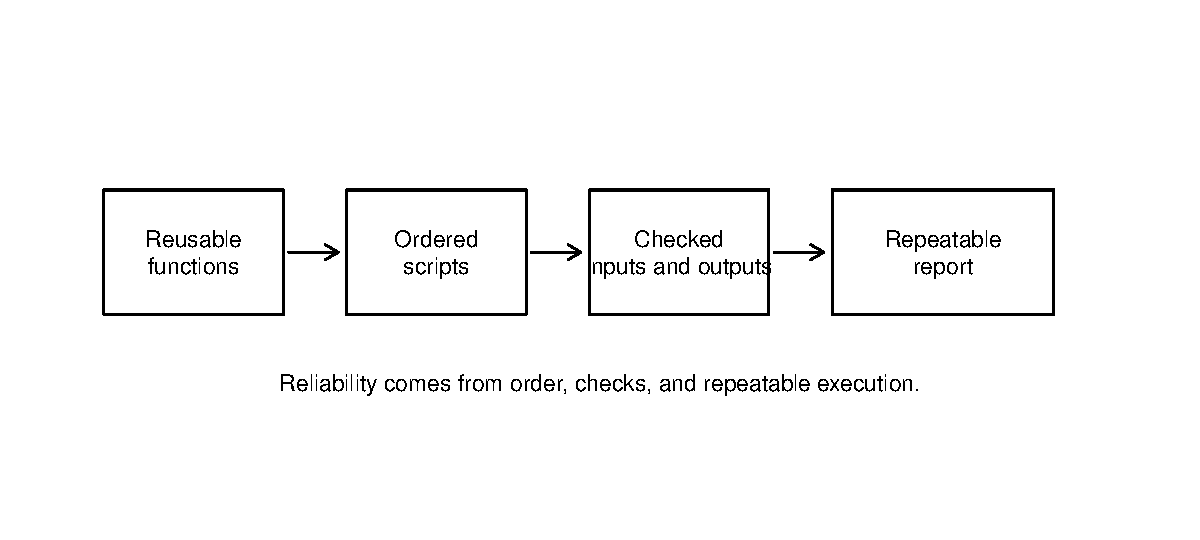
\includegraphics[width=0.92\linewidth,height=\textheight,keepaspectratio,alt={A left-to-right workflow diagram showing reusable functions becoming ordered scripts, checked inputs, controlled outputs, and a repeatable report.}]{chapters/23-reliability-and-automation_files/figure-pdf/fig-23-reusable-to-repeatable-1.pdf}

}

\caption{\label{fig-23-reusable-to-repeatable}From Reusable Tools to a
Repeatable Analytical System.}

\end{figure}%

The figure matters because it prevents a common misunderstanding. Leo is
not trying to make his project look more technical for its own sake. He
is trying to remove hidden dependence on his memory.

A workflow becomes more reliable when the next action is not a guess.

\section{Reliability Before
Automation}\label{reliability-before-automation}

Automation sounds advanced. It can make beginners imagine cloud servers,
scheduled jobs, GitHub Actions, production pipelines, and complicated
engineering systems.

That is not where Leo starts.

In this chapter, automation means something simpler and more useful:

\begin{quote}
Automation is the reduction of fragile manual repetition.
\end{quote}

Automation can begin with one script that runs steps in the right order.
It can begin with a few checks that stop the workflow when required
files are missing. It can begin with an instruction that creates an
output folder before saving a result. It can begin with a render command
that rebuilds a report from its source.

Before Leo thinks about advanced automation, he needs a reliability
vocabulary. Table~\ref{tbl-23-reliability-vocabulary} separates the key
terms that often get mixed together.

{

\begin{longtable}[]{@{}
  >{\raggedright\arraybackslash}p{(\linewidth - 4\tabcolsep) * \real{0.0948}}
  >{\raggedright\arraybackslash}p{(\linewidth - 4\tabcolsep) * \real{0.6114}}
  >{\raggedright\arraybackslash}p{(\linewidth - 4\tabcolsep) * \real{0.2938}}@{}}

\caption{\label{tbl-23-reliability-vocabulary}Core Reliability Terms for
a Beginner-Professional R Workflow.}

\tabularnewline

\toprule\noalign{}
\begin{minipage}[b]{\linewidth}\raggedright
Term
\end{minipage} & \begin{minipage}[b]{\linewidth}\raggedright
Meaning
\end{minipage} & \begin{minipage}[b]{\linewidth}\raggedright
Leo's practical question
\end{minipage} \\
\midrule\noalign{}
\endhead
\bottomrule\noalign{}
\endlastfoot
Reusable code & Code, usually a function, designed to be used more than
once without copying and rewriting it. & Can I use this tool again? \\
Repeatable workflow & A sequence of steps that can be run again in the
same intended order. & Can I run the same process again? \\
Reliable workflow & A repeatable workflow that also checks important
assumptions and reduces hidden manual decisions. & Will the process warn
me before it gives a misleading result? \\
Automation & A way of making routine steps run with fewer manual
actions. & Can I reduce repeated clicking, copying, and manual
running? \\
Reproducibility & The ability to recreate results from the same inputs,
code, and environment. & Can this result be rebuilt from its sources? \\
Dependency order & The required sequence among files, scripts, objects,
and outputs. & What must happen before this step can safely run? \\
Assumption check & A deliberate check that confirms a needed file,
folder, column, package, or object is available before later work
depends on it. & What must be true before I continue? \\
Project memory & The information a project records so Leo does not have
to remember everything alone. & What does the project know without
asking me to remember? \\

\end{longtable}

}

The distinction in Table~\ref{tbl-23-reliability-vocabulary} is more
than vocabulary. It gives Leo a practical diagnostic tool. When a
project fails, he can ask whether the problem is the code, the order,
the input, the output, the environment, or the undocumented manual step.

\section{Why Manual Workflows Break}\label{why-manual-workflows-break}

Manual work feels harmless when a project is small.

Leo opens a file. He runs one script. He changes one value. He exports
one chart. He renders one report. Nothing seems complicated.

Then the project grows.

A manual workflow begins to break for predictable reasons. The problem
is not that Leo is careless. The problem is that memory is not a
reliable workflow manager.

Table~\ref{tbl-23-workflow-risks} maps common manual workflow risks to
the reliability habit that reduces each risk.

{

\begin{longtable}[]{@{}
  >{\raggedright\arraybackslash}p{(\linewidth - 4\tabcolsep) * \real{0.2487}}
  >{\raggedright\arraybackslash}p{(\linewidth - 4\tabcolsep) * \real{0.4264}}
  >{\raggedright\arraybackslash}p{(\linewidth - 4\tabcolsep) * \real{0.3249}}@{}}

\caption{\label{tbl-23-workflow-risks}Manual Workflow Risks and the
Reliability Habits That Reduce Them.}

\tabularnewline

\toprule\noalign{}
\begin{minipage}[b]{\linewidth}\raggedright
Manual workflow risk
\end{minipage} & \begin{minipage}[b]{\linewidth}\raggedright
What can go wrong
\end{minipage} & \begin{minipage}[b]{\linewidth}\raggedright
Reliability habit
\end{minipage} \\
\midrule\noalign{}
\endhead
\bottomrule\noalign{}
\endlastfoot
Running scripts in the wrong order & Later scripts may use missing or
outdated objects. & Record and run the workflow in a visible order. \\
Trusting objects left in the Global Environment & The script may work
only because yesterday's session still contains hidden objects. &
Restart R and run from project files, not memory. \\
Forgetting to update the cleaned dataset & Summaries and plots may use
old evidence. & Make cleaned outputs part of the documented workflow. \\
Saving outputs with unclear names & Leo may not know which output
belongs to which run. & Use clear output locations and names. \\
Overwriting old results without noticing & Previous evidence may
disappear before it can be compared. & Write outputs deliberately and
avoid casual manual replacement. \\
Rendering a report from stale inputs & The report may look current while
using outdated data. & Render from source after rebuilding required
inputs. \\
Changing code without checking expected inputs & Errors may appear late
or, worse, wrong results may appear without errors. & Check assumptions
before later steps depend on them. \\
Depending on steps performed outside the project & Another reader cannot
rebuild the work from the project files. & Move hidden manual steps into
scripts or written instructions. \\

\end{longtable}

}

The risks in Table~\ref{tbl-23-workflow-risks} are not rare edge cases.
They are everyday causes of irreproducible analysis. A fragile workflow
can fail silently because nothing in the project records the proper
order of work.

This is why reliability is not a luxury. It is a form of analytical
honesty.

\section{From Files to a Workflow
Route}\label{from-files-to-a-workflow-route}

A project folder is a place. A workflow route is a path through that
place.

Leo may have many useful files:

\begin{itemize}
\tightlist
\item
  \texttt{data/raw/df\_r\_migration\_messy.csv}
\item
  \texttt{scripts/01\_import.R}
\item
  \texttt{scripts/02\_clean.R}
\item
  \texttt{scripts/03\_prepare\_analysis\_data.R}
\item
  \texttt{scripts/04\_create\_tables\_and\_figures.R}
\item
  \texttt{chapters/23-reliability-and-automation.qmd}
\item
  \texttt{data/processed/df\_analysis.rds}
\item
  \texttt{outputs/tables/}
\item
  \texttt{outputs/figures/}
\end{itemize}

Those files do not automatically tell him what to do first. Naming
helps, but naming is only the beginning. A repeatable workflow needs a
visible route.

Table~\ref{tbl-23-run-order} gives Leo a simple run-order map. It does
not require advanced pipeline software. It simply makes dependency order
explicit.

{

\begin{longtable}[]{@{}
  >{\raggedright\arraybackslash}p{(\linewidth - 8\tabcolsep) * \real{0.0269}}
  >{\raggedright\arraybackslash}p{(\linewidth - 8\tabcolsep) * \real{0.2204}}
  >{\raggedright\arraybackslash}p{(\linewidth - 8\tabcolsep) * \real{0.2151}}
  >{\raggedright\arraybackslash}p{(\linewidth - 8\tabcolsep) * \real{0.2258}}
  >{\raggedright\arraybackslash}p{(\linewidth - 8\tabcolsep) * \real{0.3118}}@{}}

\caption{\label{tbl-23-run-order}A Simple Run-Order Map for a Repeatable
R Project.}

\tabularnewline

\toprule\noalign{}
\begin{minipage}[b]{\linewidth}\raggedright
Step
\end{minipage} & \begin{minipage}[b]{\linewidth}\raggedright
Script or action
\end{minipage} & \begin{minipage}[b]{\linewidth}\raggedright
Main input
\end{minipage} & \begin{minipage}[b]{\linewidth}\raggedright
Main output
\end{minipage} & \begin{minipage}[b]{\linewidth}\raggedright
Reliability question
\end{minipage} \\
\midrule\noalign{}
\endhead
\bottomrule\noalign{}
\endlastfoot
1 & \texttt{scripts/01\_import.R} &
\texttt{data/raw/df\_r\_migration\_messy.csv} & Checked raw import & Can
R find and read the raw file? \\
2 & \texttt{scripts/02\_clean.R} & Imported raw object or saved raw
import & \texttt{data/processed/df\_r\_migration\_clean.rds} & Were
obvious data problems handled consistently? \\
3 & \texttt{scripts/03\_prepare\_analysis\_data.R} & Cleaned learner
data & \texttt{data/processed/df\_analysis.rds} & Does the analysis
dataset contain the expected variables? \\
4 & \texttt{scripts/04\_create\_tables\_and\_figures.R} & Analysis-ready
data & Tables, figures, and summary outputs & Do outputs reflect the
current data? \\
5 & \texttt{quarto\ render} & Chapter and report \texttt{.qmd} files &
Rendered book, chapter, or report & Can the document rebuild from
project files? \\

\end{longtable}

}

Table~\ref{tbl-23-run-order} gives Leo something better than memory. It
gives him an execution map. Even if he later changes the scripts, the
principle remains stable: every step should have an input, an action, an
output, and a reliability question.

\begin{tcolorbox}[enhanced jigsaw, arc=.35mm, bottomrule=.15mm, bottomtitle=1mm, breakable, colback=white, colbacktitle=quarto-callout-warning-color!10!white, colframe=quarto-callout-warning-color-frame, coltitle=black, left=2mm, leftrule=.75mm, opacityback=0, opacitybacktitle=0.6, rightrule=.15mm, title=\textcolor{quarto-callout-warning-color}{\faExclamationTriangle}\hspace{0.5em}{Project-Root Discipline}, titlerule=0mm, toprule=.15mm, toptitle=1mm]

A repeatable workflow should not depend on
\texttt{setwd("C:/Users/...")}, a Downloads folder, or a path that only
works on Leo's machine.

The safer habit is to open the project from its root folder and use
project-root relative paths such as
\texttt{data/raw/df\_r\_migration\_messy.csv},
\texttt{data/processed/df\_analysis.rds}, and
\texttt{scripts/02\_clean.R}.

\end{tcolorbox}

\begin{tcolorbox}[enhanced jigsaw, arc=.35mm, bottomrule=.15mm, bottomtitle=1mm, breakable, colback=white, colbacktitle=quarto-callout-tip-color!10!white, colframe=quarto-callout-tip-color-frame, coltitle=black, left=2mm, leftrule=.75mm, opacityback=0, opacitybacktitle=0.6, rightrule=.15mm, title=\textcolor{quarto-callout-tip-color}{\faLightbulb}\hspace{0.5em}{Lightbulb Moment}, titlerule=0mm, toprule=.15mm, toptitle=1mm]

A workflow becomes more reliable when Leo can point to the next step
without guessing.

If the order exists only in his head, the project is still depending on
memory. If the order exists in script names, a master script, a README,
or a project note, the project begins to remember for him.

\end{tcolorbox}

\section{Script-Level Discipline}\label{script-level-discipline}

A reliable workflow begins inside individual scripts.

A script should not behave like a personal scratchpad. It should tell a
future reader what it expects, what it does, and what it creates. That
future reader may be a collaborator. It may be a supervisor. Very often,
it will be Leo himself after one busy week.

A script header is a small habit with high value.
Listing~\ref{lst-23-script-header} shows a simple template Leo can
adapt.

\begin{codelisting}

\caption{\label{lst-23-script-header}A Simple Header for a Reliable
Project Script.}

\centering{

\begin{Shaded}
\begin{Highlighting}[]
\CommentTok{\# scripts/02\_clean.R}
\CommentTok{\# Purpose: Clean the raw learner migration dataset for analysis.}
\CommentTok{\# Inputs:}
\CommentTok{\#   {-} data/raw/df\_r\_migration\_messy.csv}
\CommentTok{\# Outputs:}
\CommentTok{\#   {-} data/processed/df\_r\_migration\_clean.rds}
\CommentTok{\#   {-} data/processed/df\_r\_migration\_clean.csv}
\CommentTok{\# Must run after:}
\CommentTok{\#   {-} scripts/01\_import.R, if the project saves a checked raw import first.}
\CommentTok{\# Must run before:}
\CommentTok{\#   {-} scripts/03\_prepare\_analysis\_data.R}
\CommentTok{\# Reliability notes:}
\CommentTok{\#   {-} Do not edit the raw CSV file directly.}
\CommentTok{\#   {-} Keep cleaning decisions visible in this script.}
\CommentTok{\#   {-} Save cleaned outputs to data/processed/.}
\end{Highlighting}
\end{Shaded}

}

\end{codelisting}%

The header in Listing~\ref{lst-23-script-header} is not decoration. It
answers the questions Leo asks when he returns to a project:

\begin{itemize}
\tightlist
\item
  What does this file do?
\item
  What must exist before it runs?
\item
  What does it create?
\item
  What should not be edited manually?
\item
  What depends on it later?
\end{itemize}

The header does not make the code correct by itself. It makes the script
easier to inspect, repeat, and trust.

\section{Workflow-Level Discipline}\label{workflow-level-discipline}

Script-level discipline makes each file clearer. Workflow-level
discipline makes the project clearer.

The difference matters.

A script-level question asks:

\begin{quote}
Can this script run correctly?
\end{quote}

A workflow-level question asks:

\begin{quote}
Can the project run correctly from beginning to end?
\end{quote}

Leo needs both. A clean script inside a confused workflow still leaves
him asking which file to run first. A workflow-level view shows the
dependency route.

Listing~\ref{lst-23-project-route} shows one possible project route
note. It is written as a commented planning scaffold inside a
non-evaluated R listing, so it is intentionally not executed during
rendering.

\begin{codelisting}

\caption{\label{lst-23-project-route}A Project Route Note That Makes
Workflow Order Visible.}

\centering{

\begin{Shaded}
\begin{Highlighting}[]
\CommentTok{\# Project route for the learner migration analysis}
\CommentTok{\#}
\CommentTok{\# 1. Confirm raw data exists:}
\CommentTok{\#    data/raw/df\_r\_migration\_messy.csv}
\CommentTok{\#}
\CommentTok{\# 2. Import and inspect:}
\CommentTok{\#    scripts/01\_import.R}
\CommentTok{\#}
\CommentTok{\# 3. Clean and standardise:}
\CommentTok{\#    scripts/02\_clean.R}
\CommentTok{\#}
\CommentTok{\# 4. Prepare analysis{-}ready data:}
\CommentTok{\#    scripts/03\_prepare\_analysis\_data.R}
\CommentTok{\#}
\CommentTok{\# 5. Create tables and figures:}
\CommentTok{\#    scripts/04\_create\_tables\_and\_figures.R}
\CommentTok{\#}
\CommentTok{\# 6. Render the book or report:}
\CommentTok{\#    quarto render}
\end{Highlighting}
\end{Shaded}

}

\end{codelisting}%

The route note in Listing~\ref{lst-23-project-route} does not replace
code. It helps Leo and other readers understand the workflow before
entering the code. In a small project, this can live in a
\texttt{README.md} file. In a teaching project, it may appear in a
chapter note. In a larger project, the same idea can later grow into a
more formal workflow tool.

The principle remains the same: make the order visible.

\section{Checking Assumptions Before
Running}\label{checking-assumptions-before-running}

A fragile workflow fails late. A reliable workflow tries to fail early.

This is a crucial distinction.

If the raw data file is missing, Leo should know before the cleaning
script starts. If the output folder does not exist, the script should
create it or stop with a useful message. If a required column is
missing, the workflow should not quietly continue and produce misleading
summaries.

Assumption checks are small pieces of defensive code. They do not make a
project complicated. They make failure more honest.

Listing~\ref{lst-23-required-file-check} shows a simple pattern for
checking that a required file exists before a script depends on it.

\begin{codelisting}

\caption{\label{lst-23-required-file-check}Checking That a Required
Input File Exists Before Continuing.}

\centering{

\begin{Shaded}
\begin{Highlighting}[]
\NormalTok{raw\_file }\OtherTok{\textless{}{-}} \StringTok{"data/raw/df\_r\_migration\_messy.csv"}

\ControlFlowTok{if}\NormalTok{ (}\SpecialCharTok{!}\FunctionTok{file.exists}\NormalTok{(raw\_file)) \{}
  \FunctionTok{stop}\NormalTok{(}
    \StringTok{"Required raw data file not found: "}\NormalTok{, raw\_file, }\StringTok{"}\SpecialCharTok{\textbackslash{}n}\StringTok{"}\NormalTok{,}
    \StringTok{"Place df\_r\_migration\_messy.csv in data/raw/ before running this script."}\NormalTok{,}
    \AttributeTok{call. =} \ConstantTok{FALSE}
\NormalTok{  )}
\NormalTok{\}}

\NormalTok{raw\_data }\OtherTok{\textless{}{-}} \FunctionTok{read.csv}\NormalTok{(raw\_file, }\AttributeTok{stringsAsFactors =} \ConstantTok{FALSE}\NormalTok{)}
\end{Highlighting}
\end{Shaded}

}

\end{codelisting}%

The pattern in Listing~\ref{lst-23-required-file-check} improves the
reader's experience of failure. Instead of receiving a vague error
later, Leo receives a direct message about the missing file and where it
should go.

That is reliability in practice.

\section{Checking Folders Before
Saving}\label{checking-folders-before-saving}

Files are not the only assumptions. Folders matter too.

If Leo wants to save an output to \texttt{data/processed/}, that folder
must exist. If he wants to save figures to \texttt{outputs/figures/},
that folder must exist. A beginner often creates folders manually and
then forgets which ones are required. A repeatable workflow can create
expected folders safely.

Listing~\ref{lst-23-folder-check} shows a simple folder-creation
pattern.

\begin{codelisting}

\caption{\label{lst-23-folder-check}Creating Expected Output Folders
Safely Before Saving Files.}

\centering{

\begin{Shaded}
\begin{Highlighting}[]
\NormalTok{required\_dirs }\OtherTok{\textless{}{-}} \FunctionTok{c}\NormalTok{(}
  \StringTok{"data/processed"}\NormalTok{,}
  \StringTok{"outputs/tables"}\NormalTok{,}
  \StringTok{"outputs/figures"}
\NormalTok{)}

\ControlFlowTok{for}\NormalTok{ (dir }\ControlFlowTok{in}\NormalTok{ required\_dirs) \{}
  \ControlFlowTok{if}\NormalTok{ (}\SpecialCharTok{!}\FunctionTok{dir.exists}\NormalTok{(dir)) \{}
    \FunctionTok{dir.create}\NormalTok{(dir, }\AttributeTok{recursive =} \ConstantTok{TRUE}\NormalTok{)}
\NormalTok{  \}}
\NormalTok{\}}
\end{Highlighting}
\end{Shaded}

}

\end{codelisting}%

Listing~\ref{lst-23-folder-check} is intentionally plain. Leo does not
need advanced automation to avoid a missing-folder error. He needs the
project to prepare the path before saving output.

This is one of the simplest moves from manual work to repeatable work.

\section{Checking Columns Before
Analysis}\label{checking-columns-before-analysis}

A file can exist and still be wrong.

Perhaps the wrong CSV was placed in \texttt{data/raw/}. Perhaps a column
name changed. Perhaps an earlier cleaning step dropped a variable that
the next script expects. If the analysis depends on columns such as
\texttt{learner\_id}, \texttt{study\_hours}, \texttt{project\_score},
and \texttt{completion\_status}, Leo should check that they exist before
analysis continues.

Listing~\ref{lst-23-column-check} demonstrates this habit.

\begin{codelisting}

\caption{\label{lst-23-column-check}Checking Required Columns Before
Later Analysis Depends on Them.}

\centering{

\begin{Shaded}
\begin{Highlighting}[]
\NormalTok{required\_columns }\OtherTok{\textless{}{-}} \FunctionTok{c}\NormalTok{(}
  \StringTok{"learner\_id"}\NormalTok{,}
  \StringTok{"study\_hours"}\NormalTok{,}
  \StringTok{"project\_score"}\NormalTok{,}
  \StringTok{"completion\_status"}
\NormalTok{)}

\NormalTok{missing\_columns }\OtherTok{\textless{}{-}} \FunctionTok{setdiff}\NormalTok{(required\_columns, }\FunctionTok{names}\NormalTok{(df\_analysis))}

\ControlFlowTok{if}\NormalTok{ (}\FunctionTok{length}\NormalTok{(missing\_columns) }\SpecialCharTok{\textgreater{}} \DecValTok{0}\NormalTok{) \{}
  \FunctionTok{stop}\NormalTok{(}
    \StringTok{"The analysis dataset is missing required columns: "}\NormalTok{,}
    \FunctionTok{paste}\NormalTok{(missing\_columns, }\AttributeTok{collapse =} \StringTok{", "}\NormalTok{),}
    \AttributeTok{call. =} \ConstantTok{FALSE}
\NormalTok{  )}
\NormalTok{\}}
\end{Highlighting}
\end{Shaded}

}

\end{codelisting}%

The column check in Listing~\ref{lst-23-column-check} protects the
workflow from a dangerous situation: code that runs on the wrong
structure. Reliable workflows do not simply ask whether code runs. They
ask whether the evidence has the expected shape before the code runs.

\begin{tcolorbox}[enhanced jigsaw, arc=.35mm, bottomrule=.15mm, bottomtitle=1mm, breakable, colback=white, colbacktitle=quarto-callout-warning-color!10!white, colframe=quarto-callout-warning-color-frame, coltitle=black, left=2mm, leftrule=.75mm, opacityback=0, opacitybacktitle=0.6, rightrule=.15mm, title=\textcolor{quarto-callout-warning-color}{\faExclamationTriangle}\hspace{0.5em}{Common Mistake}, titlerule=0mm, toprule=.15mm, toptitle=1mm]

Beginners often treat an error as the enemy.

In reliable analysis, a good early error is a friend. It stops the
workflow before the project produces a confident but misleading result.

\end{tcolorbox}

\section{A Master Script as a First Automation
Habit}\label{a-master-script-as-a-first-automation-habit}

A master script is one of the simplest ways to move from manual
execution to repeatable execution.

The idea is straightforward. Instead of opening several scripts and
running them one by one from memory, Leo creates one script whose job is
to run the project steps in order.

For a beginner-professional workflow, that master script might be
called:

\begin{itemize}
\tightlist
\item
  \texttt{scripts/00\_run\_project.R}
\item
  \texttt{scripts/run\_all.R}
\item
  \texttt{scripts/\_run\_workflow.R}
\end{itemize}

The name matters less than the discipline. The master script should be
easy to find, easy to read, and careful about what it runs.

Listing~\ref{lst-23-master-script} gives a beginner-friendly version. It
uses \texttt{source()} deliberately rather than casually.

\begin{codelisting}

\caption{\label{lst-23-master-script}A Beginner-Friendly Master Script
for Running Project Steps in Order.}

\centering{

\begin{Shaded}
\begin{Highlighting}[]
\CommentTok{\# scripts/00\_run\_project.R}
\CommentTok{\# Purpose: Run the learner migration workflow in the intended order.}

\FunctionTok{message}\NormalTok{(}\StringTok{"Starting learner migration workflow..."}\NormalTok{)}

\ControlFlowTok{if}\NormalTok{ (}\SpecialCharTok{!}\FunctionTok{dir.exists}\NormalTok{(}\StringTok{"scripts"}\NormalTok{) }\SpecialCharTok{||} \SpecialCharTok{!}\FunctionTok{dir.exists}\NormalTok{(}\StringTok{"data"}\NormalTok{)) \{}
  \FunctionTok{stop}\NormalTok{(}
    \StringTok{"This workflow expects to be run from the project root. "}\NormalTok{,}
    \StringTok{"Open the project folder first, then run scripts/00\_run\_project.R."}\NormalTok{,}
    \AttributeTok{call. =} \ConstantTok{FALSE}
\NormalTok{  )}
\NormalTok{\}}

\CommentTok{\# 1. Prepare expected folders}
\FunctionTok{source}\NormalTok{(}\StringTok{"scripts/00\_setup\_paths.R"}\NormalTok{)}

\CommentTok{\# 2. Import and inspect raw data}
\FunctionTok{source}\NormalTok{(}\StringTok{"scripts/01\_import.R"}\NormalTok{)}

\CommentTok{\# 3. Clean raw data}
\FunctionTok{source}\NormalTok{(}\StringTok{"scripts/02\_clean.R"}\NormalTok{)}

\CommentTok{\# 4. Prepare analysis{-}ready data}
\FunctionTok{source}\NormalTok{(}\StringTok{"scripts/03\_prepare\_analysis\_data.R"}\NormalTok{)}

\CommentTok{\# 5. Create tables and figures}
\FunctionTok{source}\NormalTok{(}\StringTok{"scripts/04\_create\_tables\_and\_figures.R"}\NormalTok{)}

\FunctionTok{message}\NormalTok{(}\StringTok{"Workflow completed. Now render the book or report from source."}\NormalTok{)}
\end{Highlighting}
\end{Shaded}

}

\end{codelisting}%

The master script in Listing~\ref{lst-23-master-script} does not make
the project advanced. It makes the project less dependent on memory. It
creates one visible place where Leo can inspect the order of work.

The master script should not become a dumping ground for every cleaning,
analysis, and plotting decision. Its main job is orchestration. The
detailed work should still live in focused scripts whose names, inputs,
outputs, and assumptions can be inspected.

This pattern also teaches humility. If running all scripts from a clean
session fails, that failure reveals a dependency problem the project was
hiding.

\section{\texorpdfstring{Controlled Use of
\texttt{source()}}{Controlled Use of source()}}\label{controlled-use-of-source}

The function \texttt{source()} tells R to run code from another script.
It is powerful, but it should be used with care.

Used well, \texttt{source()} helps Leo build a repeatable workflow. Used
carelessly, it can hide complexity and make the project harder to
inspect. The difference lies in discipline.

A controlled use of \texttt{source()} has three features:

\begin{enumerate}
\def\labelenumi{\arabic{enumi}.}
\tightlist
\item
  The sourced scripts have clear purposes.
\item
  The order is intentional.
\item
  The workflow does not depend on mysterious objects left behind in the
  Global Environment.
\end{enumerate}

Table~\ref{tbl-23-source-discipline} distinguishes helpful and risky
uses of \texttt{source()}.

{

\begin{longtable}[]{@{}
  >{\raggedright\arraybackslash}p{(\linewidth - 4\tabcolsep) * \real{0.0825}}
  >{\raggedright\arraybackslash}p{(\linewidth - 4\tabcolsep) * \real{0.4897}}
  >{\raggedright\arraybackslash}p{(\linewidth - 4\tabcolsep) * \real{0.4278}}@{}}

\caption{\label{tbl-23-source-discipline}Helpful and Risky Uses of
\texttt{source()} in Beginner-Professional R Projects.}

\tabularnewline

\toprule\noalign{}
\begin{minipage}[b]{\linewidth}\raggedright
Use of source()
\end{minipage} & \begin{minipage}[b]{\linewidth}\raggedright
Pattern
\end{minipage} & \begin{minipage}[b]{\linewidth}\raggedright
Better habit
\end{minipage} \\
\midrule\noalign{}
\endhead
\bottomrule\noalign{}
\endlastfoot
Helpful & A master script sources numbered workflow scripts in a visible
order. & Keep the order explicit and comment each major step. \\
Helpful & A script sources a small helper file that contains reusable
functions. & Keep helper files focused and avoid mixing helper functions
with analysis actions. \\
Risky & A script sources many files whose purposes and order are
unclear. & Split scripts by purpose and document the route. \\
Risky & A workflow works only because sourced scripts create hidden
objects in the Global Environment. & Save important outputs deliberately
and pass objects clearly where possible. \\

\end{longtable}

}

The point of Table~\ref{tbl-23-source-discipline} is not that
\texttt{source()} is good or bad. The point is that \texttt{source()}
should make the route clearer, not more mysterious.

\section{Clean Sessions: The Reality
Test}\label{clean-sessions-the-reality-test}

One of the most important reliability habits is simple:

\begin{quote}
Restart R and run the workflow from the project files.
\end{quote}

This habit exposes hidden dependence on memory. If a script works only
because Leo already created an object in the Global Environment, the
script is not reliable. If a report renders only because the right
object happens to exist from yesterday, the report is not reproducible.

A clean session asks the project a strict question:

\begin{quote}
Can you rebuild what you need from the files you claim to use?
\end{quote}

This is why serious work should not be judged only by whether a script
runs after a long interactive session. It should be judged by whether it
runs from a clean start.

Listing~\ref{lst-23-clean-session-test} gives Leo a simple manual test
he can perform inside RStudio or any R session.

\begin{codelisting}

\caption{\label{lst-23-clean-session-test}A Simple Clean-Session Test
for Workflow Reliability.}

\centering{

\begin{Shaded}
\begin{Highlighting}[]
\CommentTok{\# Clean{-}session reliability test}
\CommentTok{\# 1. Save all open files.}
\CommentTok{\# 2. Restart R.}
\CommentTok{\# 3. Do not manually create objects in the Console.}
\CommentTok{\# 4. Run the master script from the project root.}
\CommentTok{\# 5. Render the report or book from source.}
\CommentTok{\# 6. If something fails, fix the missing dependency in the workflow,}
\CommentTok{\#    not by manually recreating the object in the Console.}
\end{Highlighting}
\end{Shaded}

}

\end{codelisting}%

The test in Listing~\ref{lst-23-clean-session-test} is deliberately
demanding. It prevents Leo from mistaking a successful interactive
session for a repeatable project.

\begin{tcolorbox}[enhanced jigsaw, arc=.35mm, bottomrule=.15mm, bottomtitle=1mm, breakable, colback=white, colbacktitle=quarto-callout-tip-color!10!white, colframe=quarto-callout-tip-color-frame, coltitle=black, left=2mm, leftrule=.75mm, opacityback=0, opacitybacktitle=0.6, rightrule=.15mm, title=\textcolor{quarto-callout-tip-color}{\faLightbulb}\hspace{0.5em}{Reliability Habit}, titlerule=0mm, toprule=.15mm, toptitle=1mm]

When a workflow fails after restarting R, do not treat the restart as
the problem.

The restart has revealed the problem. Something important was living in
memory instead of being recorded in the project workflow.

\end{tcolorbox}

\section{Output Discipline}\label{output-discipline}

A workflow is not only about inputs and scripts. It is also about
outputs.

Output discipline means Leo knows:

\begin{itemize}
\tightlist
\item
  where outputs are saved;
\item
  which script created them;
\item
  whether they are intermediate or final;
\item
  whether they can be recreated;
\item
  whether they should be tracked in version control;
\item
  whether they should be manually edited.
\end{itemize}

This matters because output folders can become another version of the
old \texttt{final}, \texttt{final\_2}, and \texttt{real\_final} problem.
A reliable workflow should make outputs understandable.

Table~\ref{tbl-23-output-discipline} gives a practical output map for
Leo's project.

{

\begin{longtable}[]{@{}
  >{\raggedright\arraybackslash}p{(\linewidth - 4\tabcolsep) * \real{0.1832}}
  >{\raggedright\arraybackslash}p{(\linewidth - 4\tabcolsep) * \real{0.3194}}
  >{\raggedright\arraybackslash}p{(\linewidth - 4\tabcolsep) * \real{0.4974}}@{}}

\caption{\label{tbl-23-output-discipline}A Practical Output Discipline
Map for Repeatable R Workflows.}

\tabularnewline

\toprule\noalign{}
\begin{minipage}[b]{\linewidth}\raggedright
Output location
\end{minipage} & \begin{minipage}[b]{\linewidth}\raggedright
Typical contents
\end{minipage} & \begin{minipage}[b]{\linewidth}\raggedright
Reliability rule
\end{minipage} \\
\midrule\noalign{}
\endhead
\bottomrule\noalign{}
\endlastfoot
\texttt{data/processed/} & Cleaned or analysis-ready datasets & Create
from scripts; do not manually edit as if they were raw data. \\
\texttt{outputs/tables/} & CSV, RDS, or rendered tables used in reports
& Name clearly and regenerate from analysis scripts where possible. \\
\texttt{outputs/figures/} & Saved plots and image outputs & Create from
plotting scripts or report chunks; avoid manual replacement without
documentation. \\
\texttt{\_book/} or rendered report folder & Rendered HTML, PDF, EPUB,
or report files & Render from source rather than editing the rendered
output directly. \\
\texttt{logs/} & Optional run notes, validation summaries, or session
records & Use logs to document what happened, not to replace readable
code. \\

\end{longtable}

}

The map in Table~\ref{tbl-23-output-discipline} helps Leo separate
evidence from products. Raw data should be protected. Processed data
should be created by scripts. Reports should be rendered from source.
Outputs should not become secret workspaces where manual editing hides
the analytical route.

\section{Rendering as Part of the
Workflow}\label{rendering-as-part-of-the-workflow}

For a Quarto book, rendering is not an afterthought. Rendering is the
moment when source files, code chunks, outputs, cross-references,
captions, and narrative are tested together.

Leo should not treat rendering as merely pressing a button at the end.
Rendering is part of workflow reliability.

A report that cannot be rendered from source is not yet a reliable
report.

Listing~\ref{lst-23-render-commands} shows render commands Leo may run
in a Terminal from the project root, not commands he should paste into
the R Console. These commands are not evaluated in the chapter because
they are project actions rather than chapter computations.

\begin{codelisting}

\caption{\label{lst-23-render-commands}Common Quarto Render Commands for
Rebuilding Work from Source.}

\centering{

\begin{Shaded}
\begin{Highlighting}[]
\CommentTok{\# Run these commands in a Terminal from the project root. }

\CommentTok{\# Render the entire Quarto project or book }
\ExtensionTok{quarto}\NormalTok{ render}

\CommentTok{\# Render a specific chapter or document}
\ExtensionTok{quarto}\NormalTok{ render chapters/23{-}reliability{-}and{-}automation.qmd}

\CommentTok{\# Preview the project during development}
\ExtensionTok{quarto}\NormalTok{ preview}
\end{Highlighting}
\end{Shaded}

}

\end{codelisting}%

The commands in Listing~\ref{lst-23-render-commands} give Leo another
reliability habit: rebuild the product from its source. If the rendered
book exposes a broken table reference, missing figure, or failing chunk,
the render has served its purpose.

It has protected the reader.

\section{Render-Safe Thinking}\label{render-safe-thinking}

A render-safe chapter is written with the rendering process in mind.

This does not mean every code chunk must be evaluated. Some chunks are
templates, scaffolds, or commands that should not run during book
rendering. The professional habit is to decide deliberately.

For Chapter 23 and later chapters, Leo should apply a simple rule:

\begin{itemize}
\tightlist
\item
  real analysis that creates a table should usually run and receive a
  table caption;
\item
  real analysis that creates a figure should usually run and receive a
  figure caption and alt text;
\item
  templates and pseudocode should usually not run;
\item
  file-writing code should usually not run inside a book render unless
  the chapter is designed to create that file;
\item
  practice labs should usually be scaffolds that Leo runs manually.
\end{itemize}

Table~\ref{tbl-23-chunk-discipline} records this decision pattern in a
compact form.

{

\begin{longtable}[]{@{}
  >{\raggedright\arraybackslash}p{(\linewidth - 4\tabcolsep) * \real{0.2919}}
  >{\raggedright\arraybackslash}p{(\linewidth - 4\tabcolsep) * \real{0.3589}}
  >{\raggedright\arraybackslash}p{(\linewidth - 4\tabcolsep) * \real{0.3493}}@{}}

\caption{\label{tbl-23-chunk-discipline}Chunk-Execution Discipline for
Reliable Quarto Chapters from Chapter 19 Onward.}

\tabularnewline

\toprule\noalign{}
\begin{minipage}[b]{\linewidth}\raggedright
Type of chunk
\end{minipage} & \begin{minipage}[b]{\linewidth}\raggedright
Default treatment
\end{minipage} & \begin{minipage}[b]{\linewidth}\raggedright
Reliability reason
\end{minipage} \\
\midrule\noalign{}
\endhead
\bottomrule\noalign{}
\endlastfoot
Real analysis that creates a table & \texttt{eval:\ true}, with
\texttt{tbl-cap}, table label, and prose reference & The rendered
chapter proves the table can be recreated. \\
Real analysis that creates a figure & \texttt{eval:\ true}, with
\texttt{fig-cap}, \texttt{fig-alt}, figure label, and prose reference &
The rendered chapter proves the figure can be recreated and
interpreted. \\
Real code that teaches a concept but prints no useful output & Usually
\texttt{eval:\ true}, unless incomplete & The code should remain honest
unless it is only illustrative. \\
Template or pseudocode & \texttt{eval:\ false}, with \texttt{lst-label}
and prose reference if discussed & The book should not pretend a
template is a working computation. \\
Optional package demonstration & Usually \texttt{eval:\ false}, unless
the package is guaranteed in setup & Optional dependencies should not
break the render for readers. \\
File-writing or export code & Usually \texttt{eval:\ false} & A chapter
render should not unexpectedly overwrite project files. \\
App code such as Shiny & \texttt{eval:\ false} & Apps require a
different runtime context. \\
Practice-lab scaffold & Usually \texttt{eval:\ false}, so Leo can run it
manually & Practice should invite action without destabilising the book
build. \\

\end{longtable}

}

Table~\ref{tbl-23-chunk-discipline} is not a formatting preference. It
is a reliability rule. A book about reproducible work should not hide
fragile chunks, unreferenced outputs, or code that accidentally rewrites
files during rendering.

\section{Small Automation Without
Overengineering}\label{small-automation-without-overengineering}

At this point, Leo may worry that automation means learning a full
pipeline framework.

Not yet.

A beginner-professional workflow can become much more reliable with
small automation habits:

\begin{itemize}
\tightlist
\item
  one script to create expected folders;
\item
  one script to run analysis steps in order;
\item
  one render command to rebuild the document;
\item
  one checklist before submission;
\item
  one clean-session test before trusting the output.
\end{itemize}

These habits are not glamorous. They are powerful because they remove
repeated manual decisions.

Listing~\ref{lst-23-small-automation} combines several of these habits
in a small project setup script.

\begin{codelisting}

\caption{\label{lst-23-small-automation}A Small Automation Script for
Preparing Project Folders and Inputs.}

\centering{

\begin{Shaded}
\begin{Highlighting}[]
\CommentTok{\# scripts/00\_setup\_paths.R}
\CommentTok{\# Purpose: Prepare basic project paths before the workflow runs.}

\NormalTok{required\_dirs }\OtherTok{\textless{}{-}} \FunctionTok{c}\NormalTok{(}
  \StringTok{"data/raw"}\NormalTok{,}
  \StringTok{"data/processed"}\NormalTok{,}
  \StringTok{"outputs/tables"}\NormalTok{,}
  \StringTok{"outputs/figures"}
\NormalTok{)}

\ControlFlowTok{for}\NormalTok{ (dir }\ControlFlowTok{in}\NormalTok{ required\_dirs) \{}
  \ControlFlowTok{if}\NormalTok{ (}\SpecialCharTok{!}\FunctionTok{dir.exists}\NormalTok{(dir)) \{}
    \FunctionTok{dir.create}\NormalTok{(dir, }\AttributeTok{recursive =} \ConstantTok{TRUE}\NormalTok{)}
\NormalTok{  \}}
\NormalTok{\}}

\NormalTok{required\_files }\OtherTok{\textless{}{-}} \FunctionTok{c}\NormalTok{(}
  \StringTok{"data/raw/df\_r\_migration\_messy.csv"}
\NormalTok{)}

\NormalTok{missing\_files }\OtherTok{\textless{}{-}}\NormalTok{ required\_files[}\SpecialCharTok{!}\FunctionTok{file.exists}\NormalTok{(required\_files)]}

\ControlFlowTok{if}\NormalTok{ (}\FunctionTok{length}\NormalTok{(missing\_files) }\SpecialCharTok{\textgreater{}} \DecValTok{0}\NormalTok{) \{}
  \FunctionTok{stop}\NormalTok{(}
    \StringTok{"Missing required file(s): "}\NormalTok{,}
    \FunctionTok{paste}\NormalTok{(missing\_files, }\AttributeTok{collapse =} \StringTok{", "}\NormalTok{),}
    \StringTok{"}\SpecialCharTok{\textbackslash{}n}\StringTok{Place the required file(s) in the expected location before running the workflow."}\NormalTok{,}
    \AttributeTok{call. =} \ConstantTok{FALSE}
\NormalTok{  )}
\NormalTok{\}}

\FunctionTok{message}\NormalTok{(}\StringTok{"Project paths and required inputs are ready."}\NormalTok{)}
\end{Highlighting}
\end{Shaded}

}

\end{codelisting}%

The setup script in Listing~\ref{lst-23-small-automation} does not
analyse data. It prepares the ground for analysis. That is precisely why
it belongs near the beginning of a workflow. It turns assumptions into
checks.

\begin{tcolorbox}[enhanced jigsaw, arc=.35mm, bottomrule=.15mm, bottomtitle=1mm, breakable, colback=white, colbacktitle=quarto-callout-note-color!10!white, colframe=quarto-callout-note-color-frame, coltitle=black, left=2mm, leftrule=.75mm, opacityback=0, opacitybacktitle=0.6, rightrule=.15mm, title=\textcolor{quarto-callout-note-color}{\faInfo}\hspace{0.5em}{What Automation Means Here}, titlerule=0mm, toprule=.15mm, toptitle=1mm]

Automation does not mean removing human judgment.

It means reducing repeated manual actions that are easy to forget, skip,
or perform in the wrong order. Leo still decides what the workflow
should do. The project helps him run that decision consistently.

\end{tcolorbox}

\section{Validation After Running}\label{validation-after-running}

Checks before a workflow runs are important. Checks after a workflow
runs are also important.

A script may complete without an error and still create a suspicious
output. A cleaned dataset may have zero rows because a filter was too
strict. A summary may contain missing values in a key variable. A figure
may render, but from an unexpectedly small dataset.

Validation asks a simple question:

\begin{quote}
Did the workflow produce outputs that make sense?
\end{quote}

Listing~\ref{lst-23-output-validation} shows a small validation pattern
Leo can adapt after creating an analysis dataset.

\begin{codelisting}

\caption{\label{lst-23-output-validation}Checking Required Objects and
Columns Before Continuing.}

\centering{

\begin{Shaded}
\begin{Highlighting}[]
\ControlFlowTok{if}\NormalTok{ (}\SpecialCharTok{!}\FunctionTok{exists}\NormalTok{(}\StringTok{"df\_analysis"}\NormalTok{)) \{}
  \FunctionTok{stop}\NormalTok{(}
    \StringTok{"df\_analysis does not exist. Run the analysis{-}data preparation step first."}\NormalTok{,}
    \AttributeTok{call. =} \ConstantTok{FALSE}
\NormalTok{  )}
\NormalTok{\}}

\NormalTok{required\_columns }\OtherTok{\textless{}{-}} \FunctionTok{c}\NormalTok{(}
  \StringTok{"learner\_id"}\NormalTok{,}
  \StringTok{"study\_hours"}\NormalTok{,}
  \StringTok{"project\_score"}\NormalTok{,}
  \StringTok{"completion\_status"}
\NormalTok{)}

\NormalTok{missing\_columns }\OtherTok{\textless{}{-}} \FunctionTok{setdiff}\NormalTok{(required\_columns, }\FunctionTok{names}\NormalTok{(df\_analysis))}

\ControlFlowTok{if}\NormalTok{ (}\FunctionTok{length}\NormalTok{(missing\_columns) }\SpecialCharTok{\textgreater{}} \DecValTok{0}\NormalTok{) \{}
  \FunctionTok{stop}\NormalTok{(}
    \StringTok{"The analysis dataset is missing required columns: "}\NormalTok{,}
    \FunctionTok{paste}\NormalTok{(missing\_columns, }\AttributeTok{collapse =} \StringTok{", "}\NormalTok{),}
    \AttributeTok{call. =} \ConstantTok{FALSE}
\NormalTok{  )}
\NormalTok{\}}
\FunctionTok{message}\NormalTok{(}\StringTok{"df\_analysis passed basic validation checks."}\NormalTok{)}
\end{Highlighting}
\end{Shaded}

}

\end{codelisting}%

The validation pattern in Listing~\ref{lst-23-output-validation} is
intentionally modest. It does not prove the whole analysis is correct.
It protects the workflow from obvious structural failures before later
chapters, reports, or decisions depend on the output. Analytical
judgment still matters; validation only ensures that the workflow has
produced the expected object in the expected shape.

\section{Logging Without Making the Project
Heavy}\label{logging-without-making-the-project-heavy}

A log is a record of what happened.

Leo does not need a complex logging system to benefit from this idea.
Even simple messages can help him follow a workflow. The goal is not to
drown the project in technical noise. The goal is to make important
events visible.

A beginner-friendly script might report:

\begin{itemize}
\tightlist
\item
  when the workflow starts;
\item
  which input file is being read;
\item
  how many rows were imported;
\item
  where an output was saved;
\item
  whether validation checks passed;
\item
  when the workflow ends.
\end{itemize}

Listing~\ref{lst-23-simple-messages} shows this lightweight approach.

\begin{codelisting}

\caption{\label{lst-23-simple-messages}Using Simple Messages to Make
Workflow Progress Visible.}

\centering{

\begin{Shaded}
\begin{Highlighting}[]
\FunctionTok{message}\NormalTok{(}\StringTok{"Reading raw learner migration data..."}\NormalTok{)}

\NormalTok{raw\_file }\OtherTok{\textless{}{-}} \StringTok{"data/raw/df\_r\_migration\_messy.csv"}
\NormalTok{raw\_data }\OtherTok{\textless{}{-}} \FunctionTok{read.csv}\NormalTok{(raw\_file, }\AttributeTok{stringsAsFactors =} \ConstantTok{FALSE}\NormalTok{)}

\FunctionTok{message}\NormalTok{(}\StringTok{"Rows imported: "}\NormalTok{, }\FunctionTok{nrow}\NormalTok{(raw\_data))}
\FunctionTok{message}\NormalTok{(}\StringTok{"Columns imported: "}\NormalTok{, }\FunctionTok{ncol}\NormalTok{(raw\_data))}

\FunctionTok{message}\NormalTok{(}\StringTok{"Saving cleaned data to data/processed/..."}\NormalTok{)}

\CommentTok{\# saveRDS(df\_clean, "data/processed/df\_r\_migration\_clean.rds")}

\FunctionTok{message}\NormalTok{(}\StringTok{"Cleaning step completed."}\NormalTok{)}
\end{Highlighting}
\end{Shaded}

}

\end{codelisting}%

The messages in Listing~\ref{lst-23-simple-messages} should not replace
proper checks. They serve a different purpose. They help Leo see the
workflow moving through its expected stages.

\section{The Reproducibility
Checklist}\label{the-reproducibility-checklist}

Before Leo submits a report, shares a chapter, or hands a project to
someone else, he needs a final reliability check.

This is not a moral test. It is a practical protection. Many workflow
failures appear only when the project is moved, reopened, restarted, or
rendered from scratch.

Table~\ref{tbl-23-reproducibility-checklist} gives Leo a checklist he
can use before trusting a workflow.

{

\begin{longtable}[]{@{}
  >{\raggedright\arraybackslash}p{(\linewidth - 4\tabcolsep) * \real{0.2965}}
  >{\raggedright\arraybackslash}p{(\linewidth - 4\tabcolsep) * \real{0.3719}}
  >{\raggedright\arraybackslash}p{(\linewidth - 4\tabcolsep) * \real{0.3317}}@{}}

\caption{\label{tbl-23-reproducibility-checklist}A Beginner-Professional
Reproducibility Checklist Before Sharing or Submitting Work.}

\tabularnewline

\toprule\noalign{}
\begin{minipage}[b]{\linewidth}\raggedright
Check
\end{minipage} & \begin{minipage}[b]{\linewidth}\raggedright
Why it matters
\end{minipage} & \begin{minipage}[b]{\linewidth}\raggedright
Leo's question
\end{minipage} \\
\midrule\noalign{}
\endhead
\bottomrule\noalign{}
\endlastfoot
Project opens from its root folder & Relative paths depend on the
project root. & Am I working inside the project, not from a random
folder? \\
Raw data location is documented & Future readers need to know where
evidence enters the project. & Can someone find the original
evidence? \\
Scripts have a visible run order & Run order prevents memory-based
execution. & Can I tell what runs first, second, and third? \\
Important inputs are checked before use & Early checks prevent late or
silent failures. & Will the workflow stop clearly if something important
is missing? \\
Important outputs are created by code & Outputs should be reproducible
rather than manually reconstructed. & Can the project recreate this
output? \\
The workflow runs after restarting R & A clean session reveals hidden
dependencies. & Does the project work without objects left in memory? \\
The report or book renders from source & Rendering tests code,
narrative, captions, and cross-references together. & Can the document
rebuild without manual patching? \\
Tables, figures, and listings are captioned and referenced &
Reader-facing evidence should be findable and auditable. & Can a reader
trace every major output? \\
Manual steps are documented or removed & Hidden steps are a major source
of irreproducibility. & What am I still doing by hand? \\
Package environment is recorded where appropriate & A recorded
environment helps others rebuild the work later. & Can this environment
be reconstructed later? \\

\end{longtable}

}

Table~\ref{tbl-23-reproducibility-checklist} brings the chapter
together. It does not ask Leo to become a software engineer. It asks him
to make his analytical process inspectable.

\section{When to Stop Automating}\label{when-to-stop-automating}

Automation has a danger: it can become a distraction.

Leo should not automate a broken process just because automation sounds
professional. First, he should understand the work. Then he should
stabilise the order. Then he should automate the repeated parts that are
easy to forget.

A good beginner rule is:

\begin{quote}
Automate the boring, repeated, and order-sensitive steps. Keep human
judgment visible.
\end{quote}

A second rule is just as important:

\begin{quote}
If Leo cannot explain what the automation is doing, the automation is
not yet helping him.
\end{quote}

This prevents two mistakes.

The first mistake is under-automation. Leo keeps doing the same fragile
steps manually, and eventually he forgets one.

The second mistake is over-automation. Leo builds a complex system he
cannot explain, debug, or teach.

Chapter 23 belongs between those mistakes. It teaches enough automation
to make the project repeatable without turning the book into an advanced
pipeline-engineering manual.

\begin{tcolorbox}[enhanced jigsaw, arc=.35mm, bottomrule=.15mm, bottomtitle=1mm, breakable, colback=white, colbacktitle=quarto-callout-important-color!10!white, colframe=quarto-callout-important-color-frame, coltitle=black, left=2mm, leftrule=.75mm, opacityback=0, opacitybacktitle=0.6, rightrule=.15mm, title=\textcolor{quarto-callout-important-color}{\faExclamation}\hspace{0.5em}{Reliability Boundary}, titlerule=0mm, toprule=.15mm, toptitle=1mm]

This chapter is not a full lesson on CI/CD, GitHub Actions, deployment,
Shiny hosting, or advanced pipeline frameworks.

Those tools have value in the right setting. Leo's immediate need is
simpler: make the workflow run in a clear order, check assumptions,
reduce manual repetition, and rebuild outputs from source.

\end{tcolorbox}

\section{A Small Practice Lab}\label{a-small-practice-lab-10}

The best way to understand reliability is to inspect a real workflow.

Listing~\ref{lst-23-practice-lab} gives Leo a practice scaffold. It is
not evaluated because it is an activity he should perform inside his own
project.

\begin{codelisting}

\caption{\label{lst-23-practice-lab}A Practice-Lab Scaffold for Turning
a Manual Workflow into a Repeatable Workflow.}

\centering{

\begin{Shaded}
\begin{Highlighting}[]
\CommentTok{\# Practice Lab: Make the workflow remember}

\CommentTok{\# 1. List the scripts in your current project.}
\CommentTok{\#    Write them in the order you think they should run.}

\CommentTok{\# 2. For each script, answer:}
\CommentTok{\#    {-} What input does it need?}
\CommentTok{\#    {-} What output does it create?}
\CommentTok{\#    {-} What script or chapter depends on its output?}
\CommentTok{\#    {-} What could go wrong if it runs too early?}

\CommentTok{\# 3. Add a short header to each major script:}
\CommentTok{\#    {-} Purpose}
\CommentTok{\#    {-} Inputs}
\CommentTok{\#    {-} Outputs}
\CommentTok{\#    {-} Must run before}
\CommentTok{\#    {-} Must run after}

\CommentTok{\# 4. Add at least one assumption check:}
\CommentTok{\#    {-} Does the raw file exist?}
\CommentTok{\#    {-} Does the processed folder exist?}
\CommentTok{\#    {-} Does the expected column exist?}

\CommentTok{\# 5. Create a simple master script:}
\CommentTok{\#    {-} source setup script}
\CommentTok{\#    {-} source import script}
\CommentTok{\#    {-} source cleaning script}
\CommentTok{\#    {-} source analysis script}
\CommentTok{\#    {-} render the report manually after the scripts run}

\CommentTok{\# 6. Restart R.}
\CommentTok{\#    Run the workflow again from the project files.}
\CommentTok{\#    Fix the workflow whenever it depends on memory.}
\end{Highlighting}
\end{Shaded}

}

\end{codelisting}%

The practice lab in Listing~\ref{lst-23-practice-lab} is not busywork.
It is the point of the chapter. Leo is learning to move the route of
analysis out of his head and into the project.

\section{Common Beginner Mistakes}\label{common-beginner-mistakes-14}

Several mistakes appear when learners first try to make workflows
repeatable.

One common mistake is creating a master script that is only a long list
of commands copied from the Console. That does not create reliability.
It preserves confusion in a new place.

A second mistake is using \texttt{source()} to hide unclear
dependencies. If a master script sources ten files with vague names, the
project may become harder to understand, not easier.

A third mistake is saving outputs manually after running code
interactively. Manual export may feel fast, but it creates a hidden step
the project cannot repeat.

A fourth mistake is editing processed data by hand. Processed data
should normally be recreated by scripts from raw data and documented
decisions. If Leo manually edits
\texttt{data/processed/df\_analysis.csv}, the project may no longer know
how that file came to exist.

A fifth mistake is rendering only after many changes have accumulated.
Rendering early and often exposes problems while they are still small.

The correction is simple but demanding: keep the route visible, keep
assumptions checked, and keep important outputs rebuildable.

\section{Short Recap}\label{short-recap-9}

Leo began this chapter with a practical question:

\begin{quote}
``Which script should I run first?''
\end{quote}

That question revealed the difference between having scripts and having
a workflow. A folder full of files does not automatically create a
repeatable process. A reliable workflow makes order, inputs, outputs,
and assumptions visible.

He learned that reusable code is not the same as a repeatable workflow.
Reusable code helps him avoid copying logic. A repeatable workflow helps
him run the project again. A reliable workflow goes further by checking
assumptions, reducing hidden manual steps, and making outputs easier to
rebuild.

He also learned that automation does not need to begin with advanced
engineering. It can begin with script headers, file checks, folder
checks, column checks, a master script, render commands, and a
clean-session test. These habits help the project remember what Leo
should not have to carry in his head.

\section{Leo's Notebook}\label{leos-notebook-12}

\begin{itemize}
\tightlist
\item
  Correct code can still live inside a fragile workflow.
\item
  A workflow is reliable when the project knows the order, not only Leo.
\item
  Automation begins by reducing fragile manual repetition.
\item
  A good early error is protection, not failure.
\item
  Every major step should have an input, an action, an output, and a
  reliability question.
\item
  A master script is a map, not a magic wand.
\item
  If the workflow fails after restarting R, the restart has revealed a
  hidden dependency.
\item
  The best workflow is not the one Leo remembers. It is the one the
  project can run again from its own files.
\item
  Rendered reports should be rebuilt from source, not repaired by hand.
\item
  Reliability is not complexity. Reliability is disciplined
  repeatability.
\end{itemize}

\section{Glossary}\label{glossary-9}

\textbf{Assumption check}\\
A deliberate check that confirms something important is true before
later code depends on it. Examples include checking whether a file
exists, whether a folder exists, or whether required columns are
present.

\textbf{Automation}\\
The reduction of fragile manual repetition. In this chapter, automation
begins with simple scripts and commands that run routine steps in a
controlled order.

\textbf{Clean session}\\
An R session that begins without objects left over from previous work.
Restarting R before running a workflow helps reveal hidden dependencies.

\textbf{Dependency order}\\
The required sequence among inputs, scripts, intermediate outputs, and
final outputs. If one step depends on another, the earlier step must run
first.

\textbf{Master script}\\
A script whose main purpose is to run other workflow scripts in the
intended order. It helps make execution order visible.

\textbf{Output discipline}\\
The habit of saving outputs in clear, predictable locations and creating
them through code rather than hidden manual steps.

\textbf{Project memory}\\
The information stored in files, scripts, notes, checks, and project
structure so the workflow does not depend only on human memory.

\textbf{Reliable workflow}\\
A workflow that can be repeated with fewer hidden assumptions, clearer
checks, and more dependable outputs.

\textbf{Repeatable workflow}\\
A sequence of steps that can be run again in the intended order.

\textbf{Reproducibility}\\
The ability to recreate results from the same inputs, code, and
environment.

\textbf{Script-level discipline}\\
The habit of making each script clear about its purpose, inputs,
outputs, and place in the workflow.

\textbf{Workflow-level discipline}\\
The habit of making the whole project route clear, including the order
in which scripts run and how outputs are created.

\section{Chapter Outcome}\label{chapter-outcome-22}

By the end of this chapter, Leo can explain why reusable tools do not
automatically create a reliable analytical system. He can distinguish
reusable code, repeatable workflow, reliable workflow, automation, and
reproducibility. He understands that reliability depends on visible
order, checked assumptions, controlled outputs, and reduced manual
repetition.

He can create or interpret a simple workflow route. He can use script
headers to document purpose, inputs, outputs, and dependency order. He
can apply basic checks for required files, folders, and columns. He can
understand the value of a master script, controlled \texttt{source()}
calls, clean-session testing, render commands, and output discipline.

Most importantly, Leo now knows how to ask a stronger professional
question:

\begin{quote}
Can this project run again from its own files, or does it still depend
on what I remember?
\end{quote}

That question marks his movement from reusable tools to repeatable
systems.

\section{What Comes Next}\label{what-comes-next-11}

Leo can now make a workflow easier to repeat.

That is a major step. But repeatability introduces the next professional
question: what happens when the same reliable workflow becomes slow,
heavy, or difficult to scale? A small dataset may feel easy. A larger
dataset, repeated reports, heavier transformations, and slower
computations can expose new limits.

Chapter 23 has focused on reliability and automation: order, checks,
outputs, and repeatable execution. It has not taught performance. That
belongs to \href{24-performance-and-scale.qmd}{Chapter 24}.

The next chapter asks:

\begin{quote}
Once the workflow is repeatable, can it remain efficient, responsive,
and scalable as the data and tasks grow?
\end{quote}

That question moves Leo from repeatable systems to efficient systems.

\chapter{Performance and Scale: Making R Work
Efficiently}\label{performance-and-scale-making-r-work-efficiently}

\renewcommand{\thefigure}{24.\arabic{figure}}

\setcounter{figure}{0}

\renewcommand{\thetable}{24.\arabic{table}}

\setcounter{table}{0}

\section{Opening Scene: The Script Works, but It No Longer Feels
Light}\label{opening-scene-the-script-works-but-it-no-longer-feels-light}

Leo has a script that works.

That should feel like a victory, and for a while it does. The script
imports the learner data, cleans the fields, prepares a few summaries,
creates figures, and helps rebuild the report. After the work in
\hyperref[reliability-and-automation-making-workflows-repeatable]{Chapter
23}, the order is clearer. The project no longer depends only on what
Leo remembers. It has scripts, checks, outputs, and a route.

Then the project grows.

The raw file gets larger. The report now has more tables. The plots take
longer to rebuild. A transformation that felt instant with a small
dataset now pauses long enough for Leo to wonder whether R has frozen. A
colleague asks for the same report by country. Another asks for it by
learning background. Someone wants a new version after fresh data
arrives.

Nothing is obviously broken. That is what makes the problem more subtle.

The code is correct enough to run. The workflow is reliable enough to
repeat. But the work has started to feel heavy.

This is the moment when many learners make the wrong move. They search
for ``fast R code'' and begin replacing clear code with clever fragments
they barely understand. The script becomes harder to read. The output
may change. The real bottleneck may remain untouched.

Leo needs a better question.

Not, ``How do I make everything faster?''

The better question is:

\begin{quote}
What part of this workflow is slow enough, large enough, or repeated
enough to deserve attention?
\end{quote}

That question is the doorway into performance and scale.

\section{The Lightbulb Idea}\label{the-lightbulb-idea-2}

\begin{tcolorbox}[enhanced jigsaw, arc=.35mm, bottomrule=.15mm, bottomtitle=1mm, breakable, colback=white, colbacktitle=quarto-callout-tip-color!10!white, colframe=quarto-callout-tip-color-frame, coltitle=black, left=2mm, leftrule=.75mm, opacityback=0, opacitybacktitle=0.6, rightrule=.15mm, title=\textcolor{quarto-callout-tip-color}{\faLightbulb}\hspace{0.5em}{The lightbulb idea}, titlerule=0mm, toprule=.15mm, toptitle=1mm]

Performance is not about making every line faster. It is about knowing
where time, memory, and repetition actually matter.

\end{tcolorbox}

Performance is a professional judgement problem before it is a coding
problem. A slow line of code may not matter if it runs once and finishes
in less than a second. A moderately slow operation may matter greatly if
it runs inside a loop, rebuilds every report, or repeats across many
files.

Scale also has a practical meaning. It does not always mean millions of
rows or a server. Scale begins when a workflow that was comfortable at
one size becomes uncomfortable at the next size. That discomfort may
appear as waiting time, memory pressure, repeated manual work, long
render times, or fragile code that becomes harder to modify as the
project expands.

Chapter 24 therefore does not treat speed as a contest. It treats
efficiency as part of professional analytical control.

\section{Why Performance Belongs Near the End of the
Book}\label{why-performance-belongs-near-the-end-of-the-book}

Performance appears late in this book for a reason.

Earlier chapters gave Leo the basic language of R: values, types,
structures, syntax, logic, functions, and debugging. Part 3 then moved
him into data workflows: importing, cleaning, transforming, and
summarising. Part 4 helped him turn analysis into visual and narrative
communication. Part 5 has moved from reports into systems: reproducible
documents, data connections, collaboration, reusable tools, reliability,
and automation.

Only now does performance become safe to discuss.

Before Leo understands correctness, performance advice can be dangerous.
It may teach him to make wrong code faster. Before Leo understands
reproducibility, performance advice can also be distracting. It may
encourage quick local fixes that cannot be rebuilt later. Before Leo
understands workflow order, performance advice may target a small line
while the real delay comes from repeated rendering, repeated imports,
unnecessary file writing, or hidden manual steps.

Figure~\ref{fig-24-performance-position} shows the position of this
chapter in Part 5. The movement is not from slow code to fast code
alone. It is from communicable work, to traceable work, to reusable
work, to repeatable work, to efficient work, and finally to integrated
work.

\begin{Shaded}
\begin{Highlighting}[]
\FunctionTok{plot.new}\NormalTok{()}
\FunctionTok{plot.window}\NormalTok{(}\AttributeTok{xlim =} \FunctionTok{c}\NormalTok{(}\DecValTok{0}\NormalTok{, }\DecValTok{7}\NormalTok{), }\AttributeTok{ylim =} \FunctionTok{c}\NormalTok{(}\DecValTok{0}\NormalTok{, }\DecValTok{2}\NormalTok{))}
\NormalTok{steps }\OtherTok{\textless{}{-}} \FunctionTok{c}\NormalTok{(}
  \StringTok{"Reports"}\NormalTok{,}
  \StringTok{"Connections"}\NormalTok{,}
  \StringTok{"Collaboration"}\NormalTok{,}
  \StringTok{"Reusable}\SpecialCharTok{\textbackslash{}n}\StringTok{tools"}\NormalTok{,}
  \StringTok{"Reliability"}\NormalTok{,}
  \StringTok{"Performance"}\NormalTok{,}
  \StringTok{"Integration"}
\NormalTok{)}
\NormalTok{x }\OtherTok{\textless{}{-}} \FunctionTok{seq}\NormalTok{(}\FloatTok{0.7}\NormalTok{, }\FloatTok{6.3}\NormalTok{, }\AttributeTok{length.out =} \FunctionTok{length}\NormalTok{(steps))}
\NormalTok{y }\OtherTok{\textless{}{-}} \FunctionTok{rep}\NormalTok{(}\DecValTok{1}\NormalTok{, }\FunctionTok{length}\NormalTok{(steps))}

\FunctionTok{points}\NormalTok{(x, y, }\AttributeTok{pch =} \DecValTok{21}\NormalTok{, }\AttributeTok{cex =} \FloatTok{2.8}\NormalTok{)}
\FunctionTok{text}\NormalTok{(x, y, }\AttributeTok{labels =} \DecValTok{1}\SpecialCharTok{:}\FunctionTok{length}\NormalTok{(steps), }\AttributeTok{cex =} \FloatTok{0.8}\NormalTok{)}
\FunctionTok{text}\NormalTok{(x, y }\SpecialCharTok{{-}} \FloatTok{0.45}\NormalTok{, }\AttributeTok{labels =}\NormalTok{ steps, }\AttributeTok{cex =} \FloatTok{0.78}\NormalTok{)}
\FunctionTok{arrows}\NormalTok{(}
\NormalTok{  x[}\SpecialCharTok{{-}}\FunctionTok{length}\NormalTok{(x)] }\SpecialCharTok{+} \FloatTok{0.25}\NormalTok{,}
\NormalTok{  y[}\SpecialCharTok{{-}}\FunctionTok{length}\NormalTok{(y)],}
\NormalTok{  x[}\SpecialCharTok{{-}}\DecValTok{1}\NormalTok{] }\SpecialCharTok{{-}} \FloatTok{0.25}\NormalTok{,}
\NormalTok{  y[}\SpecialCharTok{{-}}\DecValTok{1}\NormalTok{],}
  \AttributeTok{length =} \FloatTok{0.08}
\NormalTok{)}
\end{Highlighting}
\end{Shaded}

\begin{figure}[H]

\centering{

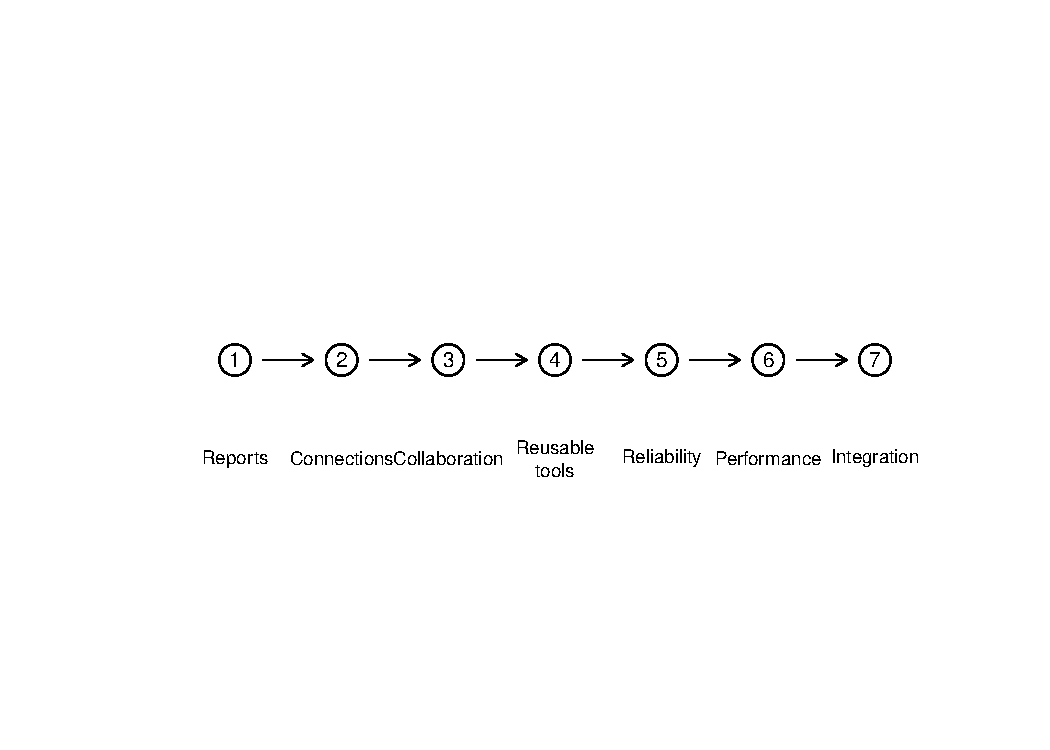
\includegraphics[width=0.9\linewidth,height=\textheight,keepaspectratio,alt={A simple horizontal flow showing Part 5 moving from reports to connections, collaboration, packages, reliability, performance, and final integration.}]{chapters/24-performance-and-scale_files/figure-pdf/fig-24-performance-position-1.pdf}

}

\caption{\label{fig-24-performance-position}The Position of Performance
and Scale within Part 5.}

\end{figure}%

This is why the chapter sits between
\hyperref[reliability-and-automation-making-workflows-repeatable]{Chapter
23} and \href{25-final-integration-project.qmd}{Chapter 25}. Chapter 23
asked whether the project could run again from its own files. Chapter 24
asks whether that repeatable project can remain efficient as the work
grows. Chapter 25 will ask Leo to connect everything into one end-to-end
analytical system.

\section{Correctness Before Speed}\label{correctness-before-speed}

The first rule of performance is almost disappointing:

\begin{quote}
Make the code correct before trying to make it fast.
\end{quote}

A fast mistake is still a mistake. A beautifully optimised pipeline that
silently changes the meaning of a variable is worse than a slow pipeline
that preserves the evidence. Performance work must therefore begin with
a known result.

Leo should first ask:

\begin{itemize}
\tightlist
\item
  Does the current code produce the correct output?
\item
  Are the variables interpreted correctly?
\item
  Are missing values handled deliberately?
\item
  Are grouping and filtering decisions documented?
\item
  Can the current result be reproduced after restarting R?
\item
  Is there a simple test, summary, or validation check that protects the
  result?
\end{itemize}

Only after these questions are settled should he ask whether the code is
too slow, too memory-heavy, or too repetitive.

\begin{tcolorbox}[enhanced jigsaw, arc=.35mm, bottomrule=.15mm, bottomtitle=1mm, breakable, colback=white, colbacktitle=quarto-callout-warning-color!10!white, colframe=quarto-callout-warning-color-frame, coltitle=black, left=2mm, leftrule=.75mm, opacityback=0, opacitybacktitle=0.6, rightrule=.15mm, title=\textcolor{quarto-callout-warning-color}{\faExclamationTriangle}\hspace{0.5em}{Do not optimise uncertainty}, titlerule=0mm, toprule=.15mm, toptitle=1mm]

If Leo does not yet trust the output, he should not begin by changing
the code for speed. First make the result trustworthy. Then make the
trustworthy result faster if the workflow genuinely needs it.

\end{tcolorbox}

Table~\ref{tbl-24-correctness-before-speed} separates three questions
that beginners often collapse into one. Keeping them apart protects the
analysis.

\begin{Shaded}
\begin{Highlighting}[]
\NormalTok{correctness\_speed }\OtherTok{\textless{}{-}} \FunctionTok{data.frame}\NormalTok{(}
  \AttributeTok{Question =} \FunctionTok{c}\NormalTok{(}
    \StringTok{"Is the result correct?"}\NormalTok{,}
    \StringTok{"Is the workflow repeatable?"}\NormalTok{,}
    \StringTok{"Is the workflow efficient enough?"}
\NormalTok{  ),}
  \AttributeTok{MainConcern =} \FunctionTok{c}\NormalTok{(}
    \StringTok{"Meaning, evidence, assumptions, and output validity"}\NormalTok{,}
    \StringTok{"Inputs, scripts, order, environment, and rebuildability"}\NormalTok{,}
    \StringTok{"Time, memory, repetition, responsiveness, and scale"}
\NormalTok{  ),}
  \AttributeTok{TypicalRisk =} \FunctionTok{c}\NormalTok{(}
    \StringTok{"Making a wrong result look polished"}\NormalTok{,}
    \StringTok{"Creating a result that cannot be recreated"}\NormalTok{,}
    \StringTok{"Optimising a small detail while the real bottleneck remains"}
\NormalTok{  ),}
  \AttributeTok{ProfessionalHabit =} \FunctionTok{c}\NormalTok{(}
    \StringTok{"Check outputs before changing strategy"}\NormalTok{,}
    \StringTok{"Run from source in a clean session"}\NormalTok{,}
    \StringTok{"Measure the bottleneck before rewriting code"}
\NormalTok{  ),}
  \AttributeTok{check.names =} \ConstantTok{FALSE}
\NormalTok{)}

\NormalTok{knitr}\SpecialCharTok{::}\FunctionTok{kable}\NormalTok{(correctness\_speed)}
\end{Highlighting}
\end{Shaded}

{

\begin{longtable}[]{@{}
  >{\raggedright\arraybackslash}p{(\linewidth - 6\tabcolsep) * \real{0.1744}}
  >{\raggedright\arraybackslash}p{(\linewidth - 6\tabcolsep) * \real{0.2872}}
  >{\raggedright\arraybackslash}p{(\linewidth - 6\tabcolsep) * \real{0.3077}}
  >{\raggedright\arraybackslash}p{(\linewidth - 6\tabcolsep) * \real{0.2308}}@{}}

\caption{\label{tbl-24-correctness-before-speed}Three Different
Questions That Should Not Be Collapsed into One.}

\tabularnewline

\toprule\noalign{}
\begin{minipage}[b]{\linewidth}\raggedright
Question
\end{minipage} & \begin{minipage}[b]{\linewidth}\raggedright
MainConcern
\end{minipage} & \begin{minipage}[b]{\linewidth}\raggedright
TypicalRisk
\end{minipage} & \begin{minipage}[b]{\linewidth}\raggedright
ProfessionalHabit
\end{minipage} \\
\midrule\noalign{}
\endhead
\bottomrule\noalign{}
\endlastfoot
Is the result correct? & Meaning, evidence, assumptions, and output
validity & Making a wrong result look polished & Check outputs before
changing strategy \\
Is the workflow repeatable? & Inputs, scripts, order, environment, and
rebuildability & Creating a result that cannot be recreated & Run from
source in a clean session \\
Is the workflow efficient enough? & Time, memory, repetition,
responsiveness, and scale & Optimising a small detail while the real
bottleneck remains & Measure the bottleneck before rewriting code \\

\end{longtable}

}

The distinction in Table~\ref{tbl-24-correctness-before-speed} is not
theoretical. It changes behaviour. If Leo has a suspicious result, he
returns to debugging and validation. If Leo cannot rebuild the project,
he returns to reliability and automation. If the result is correct and
the workflow is repeatable, but the work is now slow or heavy, he is
ready for performance thinking.

\section{What Scale Means in Practical R
Work}\label{what-scale-means-in-practical-r-work}

Scale is often described as a matter of data size. That is only partly
true.

A dataset with many rows can create scale problems. But so can many
files, many repeated reports, many plots, many joins, many groups, many
package dependencies, or many people working on the same project. Scale
appears when a strategy that worked comfortably in a small situation
begins to strain under a larger situation.

For Leo, scale may show up in six practical ways:

\begin{enumerate}
\def\labelenumi{\arabic{enumi}.}
\tightlist
\item
  The dataset grows.
\item
  The number of variables grows.
\item
  The same analysis must be repeated across groups.
\item
  Reports must be regenerated frequently.
\item
  Intermediate objects become large.
\item
  The project becomes hard to inspect, rerun, or share.
\end{enumerate}

Table~\ref{tbl-24-scale-forms} gives Leo a first map. It prevents him
from thinking that scale always means ``big data'' in the dramatic
sense.

\begin{Shaded}
\begin{Highlighting}[]
\NormalTok{scale\_forms }\OtherTok{\textless{}{-}} \FunctionTok{data.frame}\NormalTok{(}
  \AttributeTok{FormOfScale =} \FunctionTok{c}\NormalTok{(}
    \StringTok{"More rows"}\NormalTok{,}
    \StringTok{"More columns"}\NormalTok{,}
    \StringTok{"More groups"}\NormalTok{,}
    \StringTok{"More files"}\NormalTok{,}
    \StringTok{"More outputs"}\NormalTok{,}
    \StringTok{"More collaborators"}\NormalTok{,}
    \StringTok{"More frequent rebuilds"}
\NormalTok{  ),}
  \AttributeTok{WhatLeoNotices =} \FunctionTok{c}\NormalTok{(}
    \StringTok{"Imports, joins, filters, and summaries take longer"}\NormalTok{,}
    \StringTok{"Objects become harder to inspect and carry unnecessary fields"}\NormalTok{,}
    \StringTok{"The same logic is repeated across countries, cohorts, or categories"}\NormalTok{,}
    \StringTok{"Manual import and cleaning steps become fragile"}\NormalTok{,}
    \StringTok{"Tables, plots, and reports take longer to regenerate"}\NormalTok{,}
    \StringTok{"Changes become harder to track and explain"}\NormalTok{,}
    \StringTok{"Small inefficiencies are repeated many times"}
\NormalTok{  ),}
  \AttributeTok{BetterQuestion =} \FunctionTok{c}\NormalTok{(}
    \StringTok{"Can I reduce, summarise, or process only what I need?"}\NormalTok{,}
    \StringTok{"Can I select relevant columns earlier?"}\NormalTok{,}
    \StringTok{"Can I write one reusable pattern instead of copying code?"}\NormalTok{,}
    \StringTok{"Can I create a controlled import route?"}\NormalTok{,}
    \StringTok{"Can I cache or rebuild outputs deliberately?"}\NormalTok{,}
    \StringTok{"Can version control and clear structure reduce confusion?"}\NormalTok{,}
    \StringTok{"Can automation avoid repeated manual execution?"}
\NormalTok{  ),}
  \AttributeTok{check.names =} \ConstantTok{FALSE}
\NormalTok{)}

\NormalTok{knitr}\SpecialCharTok{::}\FunctionTok{kable}\NormalTok{(scale\_forms)}
\end{Highlighting}
\end{Shaded}

{

\begin{longtable}[]{@{}
  >{\raggedright\arraybackslash}p{(\linewidth - 4\tabcolsep) * \real{0.1544}}
  >{\raggedright\arraybackslash}p{(\linewidth - 4\tabcolsep) * \real{0.4564}}
  >{\raggedright\arraybackslash}p{(\linewidth - 4\tabcolsep) * \real{0.3893}}@{}}

\caption{\label{tbl-24-scale-forms}Practical Forms of Scale in an R
Project.}

\tabularnewline

\toprule\noalign{}
\begin{minipage}[b]{\linewidth}\raggedright
FormOfScale
\end{minipage} & \begin{minipage}[b]{\linewidth}\raggedright
WhatLeoNotices
\end{minipage} & \begin{minipage}[b]{\linewidth}\raggedright
BetterQuestion
\end{minipage} \\
\midrule\noalign{}
\endhead
\bottomrule\noalign{}
\endlastfoot
More rows & Imports, joins, filters, and summaries take longer & Can I
reduce, summarise, or process only what I need? \\
More columns & Objects become harder to inspect and carry unnecessary
fields & Can I select relevant columns earlier? \\
More groups & The same logic is repeated across countries, cohorts, or
categories & Can I write one reusable pattern instead of copying
code? \\
More files & Manual import and cleaning steps become fragile & Can I
create a controlled import route? \\
More outputs & Tables, plots, and reports take longer to regenerate &
Can I cache or rebuild outputs deliberately? \\
More collaborators & Changes become harder to track and explain & Can
version control and clear structure reduce confusion? \\
More frequent rebuilds & Small inefficiencies are repeated many times &
Can automation avoid repeated manual execution? \\

\end{longtable}

}

The practical lesson from Table~\ref{tbl-24-scale-forms} is that scale
can be computational, organisational, or both. A workflow can be slow
because it performs too much computation. It can also be slow because
Leo has to remember too many manual steps.

Performance is therefore not only about speed. It is about reducing
unnecessary friction.

\section{A Diagnostic Map of Common
Bottlenecks}\label{a-diagnostic-map-of-common-bottlenecks}

A bottleneck is the part of a workflow that limits the whole workflow.
If Leo wants to improve performance, he should first find the
bottleneck. Guessing is unreliable because the slowest part is not
always the most visible part.

A plot may look complex, but the delay may come from reading the same
raw file repeatedly. A model may look heavy, but the real cost may come
from creating several large intermediate objects. A pipeline may look
elegant, but it may carry twenty columns that the final report never
uses. A report may feel slow, not because any one chunk is terrible, but
because the same expensive work is repeated in several chunks.

Table~\ref{tbl-24-performance-diagnosis} gives Leo a practical
diagnostic map.

\begin{Shaded}
\begin{Highlighting}[]
\NormalTok{diagnosis\_map }\OtherTok{\textless{}{-}} \FunctionTok{data.frame}\NormalTok{(}
  \AttributeTok{Symptom =} \FunctionTok{c}\NormalTok{(}
    \StringTok{"The report takes a long time to render"}\NormalTok{,}
    \StringTok{"A transformation pauses for a long time"}\NormalTok{,}
    \StringTok{"R becomes sluggish or crashes"}\NormalTok{,}
    \StringTok{"The same code appears in many places"}\NormalTok{,}
    \StringTok{"Import is slow every time the project runs"}\NormalTok{,}
    \StringTok{"A grouped analysis is difficult to extend"}\NormalTok{,}
    \StringTok{"Code is faster but harder to trust"}
\NormalTok{  ),}
  \AttributeTok{LikelyBottleneck =} \FunctionTok{c}\NormalTok{(}
    \StringTok{"Repeated expensive chunks or unnecessary recomputation"}\NormalTok{,}
    \StringTok{"Inefficient row{-}by{-}row logic, joins, or grouping"}\NormalTok{,}
    \StringTok{"Large objects, unnecessary copies, or too many intermediate objects"}\NormalTok{,}
    \StringTok{"Manual repetition instead of a function or workflow pattern"}\NormalTok{,}
    \StringTok{"Reading large files repeatedly or reading more columns than needed"}\NormalTok{,}
    \StringTok{"Copy{-}paste structure instead of a reusable grouped pattern"}\NormalTok{,}
    \StringTok{"Optimisation was done before validation"}
\NormalTok{  ),}
  \AttributeTok{FirstResponse =} \FunctionTok{c}\NormalTok{(}
    \StringTok{"Identify which chunk is expensive before changing the whole chapter"}\NormalTok{,}
    \StringTok{"Compare a clear vectorised or grouped approach with the current approach"}\NormalTok{,}
    \StringTok{"Inspect object size and remove unused objects when safe"}\NormalTok{,}
    \StringTok{"Name the repeated action as a function or controlled script step"}\NormalTok{,}
    \StringTok{"Import once into a processed format when the workflow allows it"}\NormalTok{,}
    \StringTok{"Write one pattern that works across groups"}\NormalTok{,}
    \StringTok{"Return to correctness checks before keeping the faster version"}
\NormalTok{  ),}
  \AttributeTok{check.names =} \ConstantTok{FALSE}
\NormalTok{)}

\NormalTok{knitr}\SpecialCharTok{::}\FunctionTok{kable}\NormalTok{(diagnosis\_map)}
\end{Highlighting}
\end{Shaded}

{

\begin{longtable}[]{@{}
  >{\raggedright\arraybackslash}p{(\linewidth - 4\tabcolsep) * \real{0.2337}}
  >{\raggedright\arraybackslash}p{(\linewidth - 4\tabcolsep) * \real{0.3696}}
  >{\raggedright\arraybackslash}p{(\linewidth - 4\tabcolsep) * \real{0.3967}}@{}}

\caption{\label{tbl-24-performance-diagnosis}A Diagnostic Map for Common
Performance Bottlenecks.}

\tabularnewline

\toprule\noalign{}
\begin{minipage}[b]{\linewidth}\raggedright
Symptom
\end{minipage} & \begin{minipage}[b]{\linewidth}\raggedright
LikelyBottleneck
\end{minipage} & \begin{minipage}[b]{\linewidth}\raggedright
FirstResponse
\end{minipage} \\
\midrule\noalign{}
\endhead
\bottomrule\noalign{}
\endlastfoot
The report takes a long time to render & Repeated expensive chunks or
unnecessary recomputation & Identify which chunk is expensive before
changing the whole chapter \\
A transformation pauses for a long time & Inefficient row-by-row logic,
joins, or grouping & Compare a clear vectorised or grouped approach with
the current approach \\
R becomes sluggish or crashes & Large objects, unnecessary copies, or
too many intermediate objects & Inspect object size and remove unused
objects when safe \\
The same code appears in many places & Manual repetition instead of a
function or workflow pattern & Name the repeated action as a function or
controlled script step \\
Import is slow every time the project runs & Reading large files
repeatedly or reading more columns than needed & Import once into a
processed format when the workflow allows it \\
A grouped analysis is difficult to extend & Copy-paste structure instead
of a reusable grouped pattern & Write one pattern that works across
groups \\
Code is faster but harder to trust & Optimisation was done before
validation & Return to correctness checks before keeping the faster
version \\

\end{longtable}

}

The purpose of Table~\ref{tbl-24-performance-diagnosis} is not to make
Leo anxious. It gives him a way to slow down his diagnosis. A vague
complaint such as ``R is slow'' becomes a sharper question: ``Which part
is slow, and why?''

\section{Timing Code Without Becoming Obsessed with
Timing}\label{timing-code-without-becoming-obsessed-with-timing}

R includes simple timing tools. The most accessible is
\texttt{system.time()}. It measures how long an expression takes to run.
This is enough for early diagnosis.

Listing~\ref{lst-24-simple-timing-template} gives a small pattern Leo
can reuse when he wants to compare two versions of the same operation.
The listing is not evaluated because it is a template for his own
project.

\begin{codelisting}

\caption{\label{lst-24-simple-timing-template}A Simple Timing Template
for Comparing Two Equivalent Approaches.}

\centering{

\begin{Shaded}
\begin{Highlighting}[]
\CommentTok{\# First, confirm that both approaches produce the same result.}

\NormalTok{result\_a }\OtherTok{\textless{}{-}} \FunctionTok{approach\_a}\NormalTok{(data)}
\NormalTok{result\_b }\OtherTok{\textless{}{-}} \FunctionTok{approach\_b}\NormalTok{(data)}

\FunctionTok{stopifnot}\NormalTok{(}\FunctionTok{identical}\NormalTok{(result\_a, result\_b))}

\CommentTok{\# Then compare timing.}

\FunctionTok{system.time}\NormalTok{(\{}
\NormalTok{  result\_a }\OtherTok{\textless{}{-}} \FunctionTok{approach\_a}\NormalTok{(data)}
\NormalTok{\})}

\FunctionTok{system.time}\NormalTok{(\{}
\NormalTok{  result\_b }\OtherTok{\textless{}{-}} \FunctionTok{approach\_b}\NormalTok{(data)}
\NormalTok{\})}
\end{Highlighting}
\end{Shaded}

}

\end{codelisting}%

The important line in Listing~\ref{lst-24-simple-timing-template} is not
\texttt{system.time()}. The important line is
\texttt{stopifnot(identical(result\_a,\ result\_b))}. If the two
approaches do not produce the same result, Leo is not comparing
performance. He is comparing two different analyses.

The next example is deliberately small. It is not a universal benchmark.
It simply shows why vectorised thinking often matters.
Table~\ref{tbl-24-vectorisation-timing} compares a loop that works one
element at a time with a vectorised expression that asks R to operate on
the whole vector.

\begin{Shaded}
\begin{Highlighting}[]
\NormalTok{x }\OtherTok{\textless{}{-}} \FunctionTok{runif}\NormalTok{(}\DecValTok{200000}\NormalTok{)}

\NormalTok{loop\_time }\OtherTok{\textless{}{-}} \FunctionTok{system.time}\NormalTok{(\{}
\NormalTok{  loop\_result }\OtherTok{\textless{}{-}} \FunctionTok{numeric}\NormalTok{(}\FunctionTok{length}\NormalTok{(x))}
  \ControlFlowTok{for}\NormalTok{ (i }\ControlFlowTok{in} \FunctionTok{seq\_along}\NormalTok{(x)) \{}
\NormalTok{    loop\_result[i] }\OtherTok{\textless{}{-}} \FunctionTok{sqrt}\NormalTok{(x[i])}
\NormalTok{  \}}
\NormalTok{\})[}\StringTok{"elapsed"}\NormalTok{]}

\NormalTok{vector\_time }\OtherTok{\textless{}{-}} \FunctionTok{system.time}\NormalTok{(\{}
\NormalTok{  vector\_result }\OtherTok{\textless{}{-}} \FunctionTok{sqrt}\NormalTok{(x)}
\NormalTok{\})[}\StringTok{"elapsed"}\NormalTok{]}

\NormalTok{same\_result }\OtherTok{\textless{}{-}} \FunctionTok{isTRUE}\NormalTok{(}\FunctionTok{all.equal}\NormalTok{(loop\_result, vector\_result))}

\NormalTok{timing\_table }\OtherTok{\textless{}{-}} \FunctionTok{data.frame}\NormalTok{(}
  \AttributeTok{Approach =} \FunctionTok{c}\NormalTok{(}\StringTok{"Loop over each element"}\NormalTok{, }\StringTok{"Vectorised expression"}\NormalTok{),}
  \AttributeTok{CodeShape =} \FunctionTok{c}\NormalTok{(}
    \StringTok{"Create an output vector, then fill it one value at a time"}\NormalTok{,}
    \StringTok{"Apply \textasciigrave{}sqrt()\textasciigrave{} directly to the full vector"}
\NormalTok{  ),}
  \AttributeTok{ElapsedSeconds =} \FunctionTok{round}\NormalTok{(}\FunctionTok{c}\NormalTok{(loop\_time, vector\_time), }\DecValTok{4}\NormalTok{),}
  \AttributeTok{SameResult =} \FunctionTok{c}\NormalTok{(same\_result, same\_result),}
  \AttributeTok{check.names =} \ConstantTok{FALSE}
\NormalTok{)}

\NormalTok{knitr}\SpecialCharTok{::}\FunctionTok{kable}\NormalTok{(timing\_table)}
\end{Highlighting}
\end{Shaded}

{

\begin{longtable}[]{@{}
  >{\raggedright\arraybackslash}p{(\linewidth - 6\tabcolsep) * \real{0.2150}}
  >{\raggedright\arraybackslash}p{(\linewidth - 6\tabcolsep) * \real{0.5421}}
  >{\raggedleft\arraybackslash}p{(\linewidth - 6\tabcolsep) * \real{0.1402}}
  >{\raggedright\arraybackslash}p{(\linewidth - 6\tabcolsep) * \real{0.1028}}@{}}

\caption{\label{tbl-24-vectorisation-timing}A Small Machine-Dependent
Timing Illustration of Loop-Based and Vectorised Code.}

\tabularnewline

\toprule\noalign{}
\begin{minipage}[b]{\linewidth}\raggedright
Approach
\end{minipage} & \begin{minipage}[b]{\linewidth}\raggedright
CodeShape
\end{minipage} & \begin{minipage}[b]{\linewidth}\raggedleft
ElapsedSeconds
\end{minipage} & \begin{minipage}[b]{\linewidth}\raggedright
SameResult
\end{minipage} \\
\midrule\noalign{}
\endhead
\bottomrule\noalign{}
\endlastfoot
Loop over each element & Create an output vector, then fill it one value
at a time & 0.02 & TRUE \\
Vectorised expression & Apply \texttt{sqrt()} directly to the full
vector & 0.00 & TRUE \\

\end{longtable}

}

The numbers in Table~\ref{tbl-24-vectorisation-timing} will vary by
machine. That is expected. Leo should read the table as a diagnostic
illustration, not as a fixed promise about speed. The general lesson is
more durable: when R already knows how to operate on a vector, Leo
should usually let it do so.

\begin{tcolorbox}[enhanced jigsaw, arc=.35mm, bottomrule=.15mm, bottomtitle=1mm, breakable, colback=white, colbacktitle=quarto-callout-caution-color!10!white, colframe=quarto-callout-caution-color-frame, coltitle=black, left=2mm, leftrule=.75mm, opacityback=0, opacitybacktitle=0.6, rightrule=.15mm, title=\textcolor{quarto-callout-caution-color}{\faFire}\hspace{0.5em}{Timing is not truth by itself}, titlerule=0mm, toprule=.15mm, toptitle=1mm]

One timing run can be noisy. A small example can behave differently from
a real project. Timing is useful for diagnosis, but it should be
interpreted with judgement, not worshipped.

\end{tcolorbox}

For more advanced benchmarking, packages such as \texttt{bench} can be
useful. This chapter does not require them. The goal here is to build
the habit of measuring before rewriting.

\section{Vectorisation and the Danger of Row-by-Row
Thinking}\label{vectorisation-and-the-danger-of-row-by-row-thinking}

Many learners arrive in R with spreadsheet habits. They imagine data as
rows that must be handled one at a time. That mental model is
understandable, but it can become inefficient in R.

R is built around vectors. Many R functions expect to receive a whole
vector and return a whole vector. This is why expressions such as
\texttt{sqrt(x)}, \texttt{log(income)}, \texttt{study\_hours\ *\ 4}, and
\texttt{confidence\_score\ \textgreater{}=\ 70} work without an explicit
loop.

Vectorisation is not magic. It simply means Leo expresses the operation
in a way that matches how R is designed to work.

Consider a simple learner classification. Leo wants to identify learners
whose study hours and project scores indicate strong progress. In
row-by-row thinking, he may imagine checking each learner one at a time.
In vectorised thinking, he creates the condition across the full
columns.

\begin{Shaded}
\begin{Highlighting}[]
\ControlFlowTok{if}\NormalTok{ (}\FunctionTok{all}\NormalTok{(}\FunctionTok{c}\NormalTok{(}\StringTok{"study\_hours"}\NormalTok{, }\StringTok{"project\_score"}\NormalTok{) }\SpecialCharTok{\%in\%} \FunctionTok{names}\NormalTok{(df\_ch24))) \{}
\NormalTok{  study\_hours\_num }\OtherTok{\textless{}{-}} \FunctionTok{suppressWarnings}\NormalTok{(}\FunctionTok{as.numeric}\NormalTok{(df\_ch24}\SpecialCharTok{$}\NormalTok{study\_hours))}
\NormalTok{  project\_score\_num }\OtherTok{\textless{}{-}} \FunctionTok{suppressWarnings}\NormalTok{(}\FunctionTok{as.numeric}\NormalTok{(df\_ch24}\SpecialCharTok{$}\NormalTok{project\_score))}

\NormalTok{  df\_ch24}\SpecialCharTok{$}\NormalTok{strong\_progress }\OtherTok{\textless{}{-}} 
\NormalTok{    study\_hours\_num }\SpecialCharTok{\textgreater{}=} \FunctionTok{median}\NormalTok{(study\_hours\_num, }\AttributeTok{na.rm =} \ConstantTok{TRUE}\NormalTok{) }\SpecialCharTok{\&}
\NormalTok{    project\_score\_num }\SpecialCharTok{\textgreater{}=} \FunctionTok{median}\NormalTok{(project\_score\_num, }\AttributeTok{na.rm =} \ConstantTok{TRUE}\NormalTok{)}
\NormalTok{\}}
\end{Highlighting}
\end{Shaded}

The code above does not produce a table or figure, so it does not need a
caption. It teaches a concept and runs safely. Leo is not asking R to
visit each row manually in his code. He is asking R to evaluate a full
condition across the relevant columns.

Table~\ref{tbl-24-vectorisation-map} makes the shift more explicit.

\begin{Shaded}
\begin{Highlighting}[]
\NormalTok{vectorisation\_map }\OtherTok{\textless{}{-}} \FunctionTok{data.frame}\NormalTok{(}
  \AttributeTok{BeginnerThought =} \FunctionTok{c}\NormalTok{(}
    \StringTok{"Check the first learner, then the second, then the third"}\NormalTok{,}
    \StringTok{"Add a value to each score one row at a time"}\NormalTok{,}
    \StringTok{"Create a category by manually visiting each record"}\NormalTok{,}
    \StringTok{"Summarise each group through copied filters"}
\NormalTok{  ),}
  \AttributeTok{RThought =} \FunctionTok{c}\NormalTok{(}
    \StringTok{"Evaluate the condition across the full vector"}\NormalTok{,}
    \StringTok{"Use arithmetic directly on the full numeric vector"}\NormalTok{,}
    \StringTok{"Use a vectorised condition such as \textasciigrave{}ifelse()\textasciigrave{} or \textasciigrave{}case\_when()\textasciigrave{} where available"}\NormalTok{,}
    \StringTok{"Group once and summarise by the grouping variable"}
\NormalTok{  ),}
  \AttributeTok{WhyItScalesBetter =} \FunctionTok{c}\NormalTok{(}
    \StringTok{"The code describes the whole operation, not each manual step"}\NormalTok{,}
    \StringTok{"R uses vector operations instead of repeated user{-}level instructions"}\NormalTok{,}
    \StringTok{"The rule is easier to inspect and less likely to drift across rows"}\NormalTok{,}
    \StringTok{"The same logic works when more groups appear"}
\NormalTok{  ),}
  \AttributeTok{check.names =} \ConstantTok{FALSE}
\NormalTok{)}

\NormalTok{knitr}\SpecialCharTok{::}\FunctionTok{kable}\NormalTok{(vectorisation\_map)}
\end{Highlighting}
\end{Shaded}

{

\begin{longtable}[]{@{}
  >{\raggedright\arraybackslash}p{(\linewidth - 4\tabcolsep) * \real{0.2780}}
  >{\raggedright\arraybackslash}p{(\linewidth - 4\tabcolsep) * \real{0.3854}}
  >{\raggedright\arraybackslash}p{(\linewidth - 4\tabcolsep) * \real{0.3366}}@{}}

\caption{\label{tbl-24-vectorisation-map}Moving from Row-by-Row Thinking
to Vectorised R Thinking.}

\tabularnewline

\toprule\noalign{}
\begin{minipage}[b]{\linewidth}\raggedright
BeginnerThought
\end{minipage} & \begin{minipage}[b]{\linewidth}\raggedright
RThought
\end{minipage} & \begin{minipage}[b]{\linewidth}\raggedright
WhyItScalesBetter
\end{minipage} \\
\midrule\noalign{}
\endhead
\bottomrule\noalign{}
\endlastfoot
Check the first learner, then the second, then the third & Evaluate the
condition across the full vector & The code describes the whole
operation, not each manual step \\
Add a value to each score one row at a time & Use arithmetic directly on
the full numeric vector & R uses vector operations instead of repeated
user-level instructions \\
Create a category by manually visiting each record & Use a vectorised
condition such as \texttt{ifelse()} or \texttt{case\_when()} where
available & The rule is easier to inspect and less likely to drift
across rows \\
Summarise each group through copied filters & Group once and summarise
by the grouping variable & The same logic works when more groups
appear \\

\end{longtable}

}

The mental shift in Table~\ref{tbl-24-vectorisation-map} also improves
readability. A clear vectorised expression often says what Leo means
more directly than a long loop.

This does not mean loops are forbidden. Loops are useful when each step
depends on the previous step, when a task is genuinely iterative, or
when Leo is coordinating repeated operations carefully. The mistake is
not using a loop. The mistake is using row-by-row code when a clearer
vectorised expression already exists.

\section{Runtime Growth: Why Small Examples Can
Mislead}\label{runtime-growth-why-small-examples-can-mislead}

A script can feel fast with 100 rows and slow with 100,000 rows. That
does not mean R has become irrational. It often means the cost of an
operation grows with the size of the input.

Figure~\ref{fig-24-runtime-growth} gives a conceptual picture of runtime
growth. The curves are not measured from a specific computer. They are a
teaching illustration that helps Leo understand why some strategies
become uncomfortable faster than others.

\begin{Shaded}
\begin{Highlighting}[]
\NormalTok{n }\OtherTok{\textless{}{-}} \FunctionTok{seq}\NormalTok{(}\DecValTok{1}\NormalTok{, }\DecValTok{100}\NormalTok{, }\AttributeTok{by =} \DecValTok{1}\NormalTok{)}
\NormalTok{linear }\OtherTok{\textless{}{-}}\NormalTok{ n }\SpecialCharTok{/} \FunctionTok{max}\NormalTok{(n)}
\NormalTok{nlogn }\OtherTok{\textless{}{-}}\NormalTok{ (n }\SpecialCharTok{*} \FunctionTok{log}\NormalTok{(n }\SpecialCharTok{+} \DecValTok{1}\NormalTok{)) }\SpecialCharTok{/} \FunctionTok{max}\NormalTok{(n }\SpecialCharTok{*} \FunctionTok{log}\NormalTok{(n }\SpecialCharTok{+} \DecValTok{1}\NormalTok{))}
\NormalTok{quadratic }\OtherTok{\textless{}{-}}\NormalTok{ (n}\SpecialCharTok{\^{}}\DecValTok{2}\NormalTok{) }\SpecialCharTok{/} \FunctionTok{max}\NormalTok{(n}\SpecialCharTok{\^{}}\DecValTok{2}\NormalTok{)}

\FunctionTok{matplot}\NormalTok{(}
\NormalTok{  n,}
  \FunctionTok{cbind}\NormalTok{(linear, nlogn, quadratic),}
  \AttributeTok{type =} \StringTok{"l"}\NormalTok{,}
  \AttributeTok{lty =} \FunctionTok{c}\NormalTok{(}\DecValTok{1}\NormalTok{, }\DecValTok{2}\NormalTok{, }\DecValTok{3}\NormalTok{),}
  \AttributeTok{lwd =} \DecValTok{2}\NormalTok{,}
  \AttributeTok{xlab =} \StringTok{"Work size"}\NormalTok{,}
  \AttributeTok{ylab =} \StringTok{"Relative runtime"}\NormalTok{,}
  \AttributeTok{main =} \StringTok{"Conceptual Runtime Growth"}
\NormalTok{)}
\FunctionTok{legend}\NormalTok{(}
  \StringTok{"topleft"}\NormalTok{,}
  \AttributeTok{legend =} \FunctionTok{c}\NormalTok{(}\StringTok{"Linear"}\NormalTok{, }\StringTok{"n log n"}\NormalTok{, }\StringTok{"Quadratic"}\NormalTok{),}
  \AttributeTok{lty =} \FunctionTok{c}\NormalTok{(}\DecValTok{1}\NormalTok{, }\DecValTok{2}\NormalTok{, }\DecValTok{3}\NormalTok{),}
  \AttributeTok{lwd =} \DecValTok{2}\NormalTok{,}
  \AttributeTok{bty =} \StringTok{"n"}
\NormalTok{)}
\end{Highlighting}
\end{Shaded}

\begin{figure}[H]

\centering{

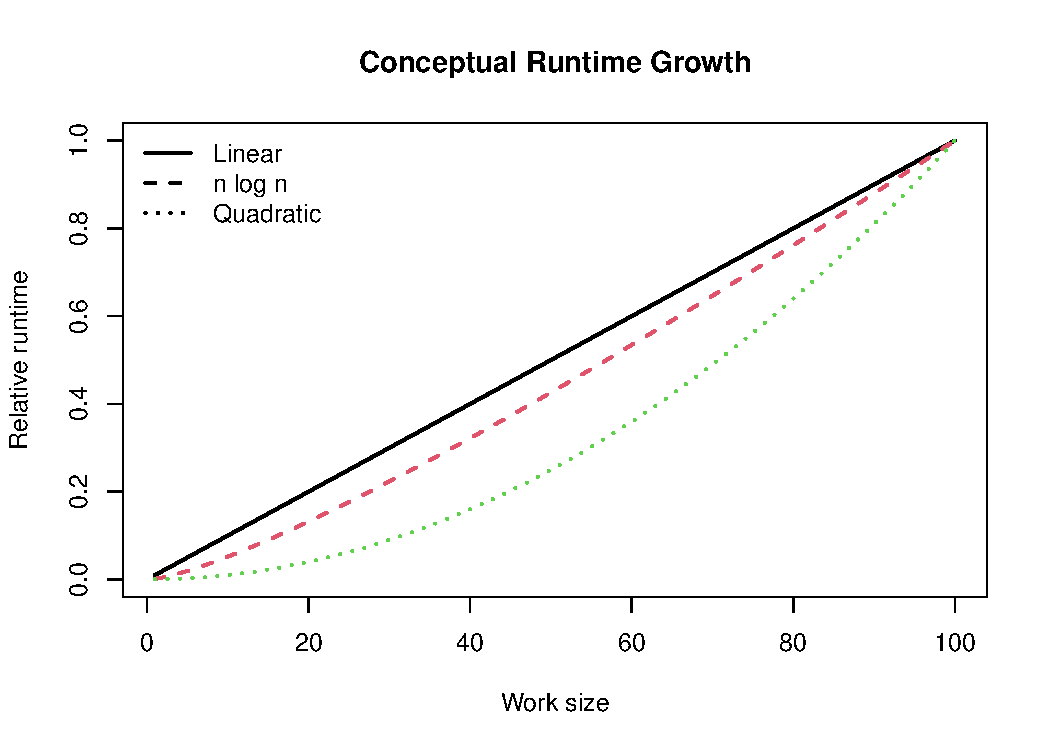
\includegraphics[width=0.9\linewidth,height=\textheight,keepaspectratio,alt={A line chart showing three conceptual runtime patterns. Linear growth rises slowly, n log n growth rises moderately, and quadratic growth rises sharply as work size increases.}]{chapters/24-performance-and-scale_files/figure-pdf/fig-24-runtime-growth-1.pdf}

}

\caption{\label{fig-24-runtime-growth}A Conceptual Illustration of How
Different Runtime Patterns Grow as Work Size Increases.}

\end{figure}%

The lesson from Figure~\ref{fig-24-runtime-growth} is not that Leo must
learn formal algorithm analysis before doing data work. The lesson is
more practical: a strategy that repeats unnecessary work may look
harmless in a small example, then become painful when the input grows.

This is why performance thinking begins with repeated work. A small
inefficiency inside a repeated operation can become a large delay.

\section{Memory, Copying, and Object
Size}\label{memory-copying-and-object-size}

Time is not the only performance issue. Memory matters too.

In R, objects live in memory during a session. If Leo creates several
large copies of the same dataset, memory use can grow quickly. This is
not usually a problem with small teaching examples. It can become a
problem when a project carries many large intermediate objects, imports
unnecessary columns, or repeatedly saves and reloads heavy objects.

A practical first step is to inspect object size.
Table~\ref{tbl-24-object-size} uses the current analysis dataset when
available. If the project data is not present during rendering, the
chapter uses a small teaching fallback created in the setup chunk.

\begin{Shaded}
\begin{Highlighting}[]
\NormalTok{preferred\_columns }\OtherTok{\textless{}{-}} \FunctionTok{intersect}\NormalTok{(}
  \FunctionTok{c}\NormalTok{(}
    \StringTok{"learner\_id"}\NormalTok{,}
    \StringTok{"country"}\NormalTok{,}
    \StringTok{"background"}\NormalTok{,}
    \StringTok{"study\_hours"}\NormalTok{,}
    \StringTok{"lessons\_completed"}\NormalTok{,}
    \StringTok{"confidence\_score"}\NormalTok{,}
    \StringTok{"project\_score"}\NormalTok{,}
    \StringTok{"completion\_status"}\NormalTok{,}
    \StringTok{"strong\_progress"}
\NormalTok{  ),}
  \FunctionTok{names}\NormalTok{(df\_ch24)}
\NormalTok{)}

\ControlFlowTok{if}\NormalTok{ (}\FunctionTok{length}\NormalTok{(preferred\_columns) }\SpecialCharTok{==} \DecValTok{0}\NormalTok{) \{}
\NormalTok{  preferred\_columns }\OtherTok{\textless{}{-}} \FunctionTok{names}\NormalTok{(df\_ch24)[}\FunctionTok{seq\_len}\NormalTok{(}\FunctionTok{min}\NormalTok{(}\DecValTok{6}\NormalTok{, }\FunctionTok{ncol}\NormalTok{(df\_ch24)))]}
\NormalTok{\}}

\NormalTok{df\_ch24\_subset }\OtherTok{\textless{}{-}}\NormalTok{ df\_ch24[, preferred\_columns, drop }\OtherTok{=} \ConstantTok{FALSE}\NormalTok{]}

\NormalTok{object\_size\_table }\OtherTok{\textless{}{-}} \FunctionTok{data.frame}\NormalTok{(}
  \AttributeTok{Object =} \FunctionTok{c}\NormalTok{(}\StringTok{"Full chapter dataset"}\NormalTok{, }\StringTok{"Selected working columns"}\NormalTok{),}
  \AttributeTok{Rows =} \FunctionTok{c}\NormalTok{(}\FunctionTok{nrow}\NormalTok{(df\_ch24), }\FunctionTok{nrow}\NormalTok{(df\_ch24\_subset)),}
  \AttributeTok{Columns =} \FunctionTok{c}\NormalTok{(}\FunctionTok{ncol}\NormalTok{(df\_ch24), }\FunctionTok{ncol}\NormalTok{(df\_ch24\_subset)),}
  \AttributeTok{ApproximateMemory =} \FunctionTok{c}\NormalTok{(}
    \FunctionTok{format}\NormalTok{(}\FunctionTok{object.size}\NormalTok{(df\_ch24), }\AttributeTok{units =} \StringTok{"auto"}\NormalTok{),}
    \FunctionTok{format}\NormalTok{(}\FunctionTok{object.size}\NormalTok{(df\_ch24\_subset), }\AttributeTok{units =} \StringTok{"auto"}\NormalTok{)}
\NormalTok{  ),}
  \AttributeTok{check.names =} \ConstantTok{FALSE}
\NormalTok{)}

\NormalTok{knitr}\SpecialCharTok{::}\FunctionTok{kable}\NormalTok{(object\_size\_table)}
\end{Highlighting}
\end{Shaded}

{

\begin{longtable}[]{@{}lrrl@{}}

\caption{\label{tbl-24-object-size}A Small Object-Size Check Using the
Chapter Dataset.}

\tabularnewline

\toprule\noalign{}
Object & Rows & Columns & ApproximateMemory \\
\midrule\noalign{}
\endhead
\bottomrule\noalign{}
\endlastfoot
Full chapter dataset & 584 & 27 & 143.4 Kb \\
Selected working columns & 584 & 9 & 73.2 Kb \\

\end{longtable}

}

Table~\ref{tbl-24-object-size} is intentionally modest. It does not tell
Leo to cut every dataset down immediately. It teaches a habit: inspect
what the workflow is carrying. If a report needs five columns, carrying
twenty-eight columns through every step may not be harmful at this size,
but the habit can become expensive at larger sizes.

\begin{tcolorbox}[enhanced jigsaw, arc=.35mm, bottomrule=.15mm, bottomtitle=1mm, breakable, colback=white, colbacktitle=quarto-callout-tip-color!10!white, colframe=quarto-callout-tip-color-frame, coltitle=black, left=2mm, leftrule=.75mm, opacityback=0, opacitybacktitle=0.6, rightrule=.15mm, title=\textcolor{quarto-callout-tip-color}{\faLightbulb}\hspace{0.5em}{A practical memory habit}, titlerule=0mm, toprule=.15mm, toptitle=1mm]

Select the columns needed for a task when the purpose is clear. Do not
remove useful evidence too early, but do not carry unnecessary weight
through every later step simply because the full dataset was imported.

\end{tcolorbox}

The same judgement applies to intermediate objects. Clear names such as
\texttt{raw\_migration}, \texttt{df\_r\_migration}, and
\texttt{df\_analysis} help preserve workflow meaning. But creating many
nearly identical objects can make both memory and interpretation harder.
Leo should keep intermediate objects when they mark meaningful workflow
stages. He should avoid keeping them merely because he is afraid to
overwrite anything.

The reliable solution is not reckless overwriting. It is controlled
staging: raw data stays raw, processed data is saved deliberately,
analysis-ready data is created through code, and temporary objects are
removed when they no longer serve a purpose.

\section{Efficient Pipelines Without Sacrificing
Clarity}\label{efficient-pipelines-without-sacrificing-clarity}

Efficiency should not destroy readability.

A pipeline that no one understands is not a professional achievement. A
faster script that Leo cannot safely modify next month is a liability.
The goal is to write code that is clear enough to audit and efficient
enough for the work it must do.

This is especially important with \texttt{dplyr} pipelines. In the
earlier data chapters, pipelines helped Leo express a sequence of data
actions. That remains valuable. The question in Chapter 24 is not
whether pipelines are good or bad. The question is whether the pipeline
is doing unnecessary work.

A clear pipeline usually scales better when it:

\begin{itemize}
\tightlist
\item
  selects only needed columns once the purpose is known
\item
  filters irrelevant rows before expensive summaries when appropriate
\item
  groups deliberately, then ungroups when grouping is no longer needed
\item
  avoids repeating the same transformation in several places
\item
  creates named helper functions for repeated logic
\item
  checks outputs after any major rewrite
\end{itemize}

Table~\ref{tbl-24-pipeline-discipline} summarises the difference between
clear inefficient code, clever risky code, and disciplined efficient
code.

\begin{Shaded}
\begin{Highlighting}[]
\NormalTok{pipeline\_discipline }\OtherTok{\textless{}{-}} \FunctionTok{data.frame}\NormalTok{(}
  \AttributeTok{Pattern =} \FunctionTok{c}\NormalTok{(}
    \StringTok{"Clear but wasteful"}\NormalTok{,}
    \StringTok{"Fast but obscure"}\NormalTok{,}
    \StringTok{"Disciplined and efficient"}
\NormalTok{  ),}
  \AttributeTok{WhatItLooksLike =} \FunctionTok{c}\NormalTok{(}
    \StringTok{"The same summaries are recalculated in many chunks"}\NormalTok{,}
    \StringTok{"Dense code uses unfamiliar tricks without explanation"}\NormalTok{,}
    \StringTok{"The workflow removes unnecessary repetition while keeping intent visible"}
\NormalTok{  ),}
  \AttributeTok{Risk =} \FunctionTok{c}\NormalTok{(}
    \StringTok{"The project becomes slow as outputs multiply"}\NormalTok{,}
    \StringTok{"Future readers cannot safely audit or revise the work"}\NormalTok{,}
    \StringTok{"Requires judgement about what should be abstracted or simplified"}
\NormalTok{  ),}
  \AttributeTok{BetterHabit =} \FunctionTok{c}\NormalTok{(}
    \StringTok{"Save or reuse meaningful intermediate summaries"}\NormalTok{,}
    \StringTok{"Explain the strategy or choose a clearer approach"}\NormalTok{,}
    \StringTok{"Make the repeated action visible through a function, script, or named object"}
\NormalTok{  ),}
  \AttributeTok{check.names =} \ConstantTok{FALSE}
\NormalTok{)}

\NormalTok{knitr}\SpecialCharTok{::}\FunctionTok{kable}\NormalTok{(pipeline\_discipline)}
\end{Highlighting}
\end{Shaded}

{

\begin{longtable}[]{@{}
  >{\raggedright\arraybackslash}p{(\linewidth - 6\tabcolsep) * \real{0.1079}}
  >{\raggedright\arraybackslash}p{(\linewidth - 6\tabcolsep) * \real{0.3029}}
  >{\raggedright\arraybackslash}p{(\linewidth - 6\tabcolsep) * \real{0.2697}}
  >{\raggedright\arraybackslash}p{(\linewidth - 6\tabcolsep) * \real{0.3195}}@{}}

\caption{\label{tbl-24-pipeline-discipline}Balancing Clarity and
Efficiency in Data Pipelines.}

\tabularnewline

\toprule\noalign{}
\begin{minipage}[b]{\linewidth}\raggedright
Pattern
\end{minipage} & \begin{minipage}[b]{\linewidth}\raggedright
WhatItLooksLike
\end{minipage} & \begin{minipage}[b]{\linewidth}\raggedright
Risk
\end{minipage} & \begin{minipage}[b]{\linewidth}\raggedright
BetterHabit
\end{minipage} \\
\midrule\noalign{}
\endhead
\bottomrule\noalign{}
\endlastfoot
Clear but wasteful & The same summaries are recalculated in many chunks
& The project becomes slow as outputs multiply & Save or reuse
meaningful intermediate summaries \\
Fast but obscure & Dense code uses unfamiliar tricks without explanation
& Future readers cannot safely audit or revise the work & Explain the
strategy or choose a clearer approach \\
Disciplined and efficient & The workflow removes unnecessary repetition
while keeping intent visible & Requires judgement about what should be
abstracted or simplified & Make the repeated action visible through a
function, script, or named object \\

\end{longtable}

}

The middle row in Table~\ref{tbl-24-pipeline-discipline} is the trap.
Leo should not confuse cleverness with professionalism. Good performance
work makes the project easier to run and still possible to understand.

\section{Larger-Than-Comfortable Data: Practical
Options}\label{larger-than-comfortable-data-practical-options}

Most R users do not begin with truly massive data. They begin with data
that becomes larger than their current habits can comfortably handle.
This may mean a CSV file that takes too long to read, a join that
strains memory, or a report that repeats expensive work.

Before reaching for advanced tools, Leo should ask whether a simpler
improvement is enough.

Can he filter earlier? Can he select fewer columns? Can he avoid reading
the same file repeatedly? Can he save a processed version after
cleaning? Can he summarise before plotting? Can he move repeated code
into a function from the habits developed in
\hyperref[from-functions-to-packages-building-reusable-r-tools]{Chapter
22}?

If the answer is no, then specialised tools may be appropriate.
Table~\ref{tbl-24-tool-options} gives a careful map. It does not tell
Leo to use every tool. It helps him know when each class of tool becomes
relevant.

\begin{Shaded}
\begin{Highlighting}[]
\NormalTok{tool\_options }\OtherTok{\textless{}{-}} \FunctionTok{data.frame}\NormalTok{(}
  \AttributeTok{Option =} \FunctionTok{c}\NormalTok{(}
    \StringTok{"Clear base R"}\NormalTok{,}
    \StringTok{"Tidyverse workflow"}\NormalTok{,}
    \StringTok{"data.table"}\NormalTok{,}
    \StringTok{"Database{-}backed workflow"}\NormalTok{,}
    \StringTok{"Arrow{-}style columnar workflow"}\NormalTok{,}
    \StringTok{"Parallel computing"}\NormalTok{,}
    \StringTok{"Project redesign"}
\NormalTok{  ),}
  \AttributeTok{BestWhen =} \FunctionTok{c}\NormalTok{(}
    \StringTok{"The task is small, direct, and easy to express with built{-}in functions"}\NormalTok{,}
    \StringTok{"The priority is readable data manipulation and communicable analysis"}\NormalTok{,}
    \StringTok{"Large in{-}memory tables require fast filtering, grouping, joining, or updating"}\NormalTok{,}
    \StringTok{"The data is too large or too centralised to load fully into R"}\NormalTok{,}
    \StringTok{"The workflow benefits from columnar storage, partitioned data, or cross{-}tool access"}\NormalTok{,}
    \StringTok{"Independent tasks are large enough to justify worker setup and coordination"}\NormalTok{,}
    \StringTok{"The bottleneck is repeated manual or structural work rather than one slow function"}
\NormalTok{  ),}
  \AttributeTok{Caution =} \FunctionTok{c}\NormalTok{(}
    \StringTok{"Can become hard to read if over{-}compressed"}\NormalTok{,}
    \StringTok{"Can become slow if the same expensive work is repeated without need"}\NormalTok{,}
    \StringTok{"Requires learning a different syntax and reference semantics"}\NormalTok{,}
    \StringTok{"Requires database knowledge and careful query design"}\NormalTok{,}
    \StringTok{"Adds a storage and tooling layer that beginners should not adopt casually"}\NormalTok{,}
    \StringTok{"Can increase memory use, complexity, and reproducibility demands"}\NormalTok{,}
    \StringTok{"Requires discipline, not a new package"}
\NormalTok{  ),}
  \AttributeTok{RenderingRoleInThisChapter =} \FunctionTok{c}\NormalTok{(}
    \StringTok{"Safe for evaluated examples"}\NormalTok{,}
    \StringTok{"Appropriate where already used in the book setup"}\NormalTok{,}
    \StringTok{"Optional demonstration only"}\NormalTok{,}
    \StringTok{"Optional demonstration only"}\NormalTok{,}
    \StringTok{"Optional demonstration only"}\NormalTok{,}
    \StringTok{"Optional demonstration only"}\NormalTok{,}
    \StringTok{"Central professional habit"}
\NormalTok{  ),}
  \AttributeTok{check.names =} \ConstantTok{FALSE}
\NormalTok{)}

\NormalTok{knitr}\SpecialCharTok{::}\FunctionTok{kable}\NormalTok{(tool\_options)}
\end{Highlighting}
\end{Shaded}

{

\begin{longtable}[]{@{}
  >{\raggedright\arraybackslash}p{(\linewidth - 6\tabcolsep) * \real{0.1266}}
  >{\raggedright\arraybackslash}p{(\linewidth - 6\tabcolsep) * \real{0.3544}}
  >{\raggedright\arraybackslash}p{(\linewidth - 6\tabcolsep) * \real{0.3122}}
  >{\raggedright\arraybackslash}p{(\linewidth - 6\tabcolsep) * \real{0.2068}}@{}}

\caption{\label{tbl-24-tool-options}A Practical Map of R Performance
Options as Projects Grow.}

\tabularnewline

\toprule\noalign{}
\begin{minipage}[b]{\linewidth}\raggedright
Option
\end{minipage} & \begin{minipage}[b]{\linewidth}\raggedright
BestWhen
\end{minipage} & \begin{minipage}[b]{\linewidth}\raggedright
Caution
\end{minipage} & \begin{minipage}[b]{\linewidth}\raggedright
RenderingRoleInThisChapter
\end{minipage} \\
\midrule\noalign{}
\endhead
\bottomrule\noalign{}
\endlastfoot
Clear base R & The task is small, direct, and easy to express with
built-in functions & Can become hard to read if over-compressed & Safe
for evaluated examples \\
Tidyverse workflow & The priority is readable data manipulation and
communicable analysis & Can become slow if the same expensive work is
repeated without need & Appropriate where already used in the book
setup \\
data.table & Large in-memory tables require fast filtering, grouping,
joining, or updating & Requires learning a different syntax and
reference semantics & Optional demonstration only \\
Database-backed workflow & The data is too large or too centralised to
load fully into R & Requires database knowledge and careful query design
& Optional demonstration only \\
Arrow-style columnar workflow & The workflow benefits from columnar
storage, partitioned data, or cross-tool access & Adds a storage and
tooling layer that beginners should not adopt casually & Optional
demonstration only \\
Parallel computing & Independent tasks are large enough to justify
worker setup and coordination & Can increase memory use, complexity, and
reproducibility demands & Optional demonstration only \\
Project redesign & The bottleneck is repeated manual or structural work
rather than one slow function & Requires discipline, not a new package &
Central professional habit \\

\end{longtable}

}

The strongest line in Table~\ref{tbl-24-tool-options} may be the last
one. Sometimes the problem is not that Leo lacks a faster package. The
problem is that the workflow is poorly shaped. A poorly shaped workflow
can make any package feel slow.

\begin{tcolorbox}[enhanced jigsaw, arc=.35mm, bottomrule=.15mm, bottomtitle=1mm, breakable, colback=white, colbacktitle=quarto-callout-note-color!10!white, colframe=quarto-callout-note-color-frame, coltitle=black, left=2mm, leftrule=.75mm, opacityback=0, opacitybacktitle=0.6, rightrule=.15mm, title=\textcolor{quarto-callout-note-color}{\faInfo}\hspace{0.5em}{Optional tools are not beginner requirements}, titlerule=0mm, toprule=.15mm, toptitle=1mm]

Packages such as \texttt{data.table}, \texttt{arrow}, and
\texttt{duckdb} can be powerful. This chapter mentions them because
professionals may encounter them as projects grow. They are not required
for Leo to understand performance thinking, and the optional examples
below are not evaluated during rendering.

\end{tcolorbox}

Listing~\ref{lst-24-optional-data-table-pattern} shows the kind of
pattern Leo may later see in \texttt{data.table}. It is included for
recognition, not as a required dependency.

\begin{codelisting}

\caption{\label{lst-24-optional-data-table-pattern}An Optional
data.table Pattern for Fast Grouped Summaries.}

\centering{

\begin{Shaded}
\begin{Highlighting}[]
\FunctionTok{library}\NormalTok{(data.table)}

\NormalTok{learner\_dt }\OtherTok{\textless{}{-}} \FunctionTok{as.data.table}\NormalTok{(df\_analysis)}

\NormalTok{country\_summary }\OtherTok{\textless{}{-}}\NormalTok{ learner\_dt[}
\NormalTok{  ,}
\NormalTok{  .(}
    \AttributeTok{learners =}\NormalTok{ .N,}
    \AttributeTok{average\_project\_score =} \FunctionTok{mean}\NormalTok{(project\_score, }\AttributeTok{na.rm =} \ConstantTok{TRUE}\NormalTok{),}
    \AttributeTok{average\_study\_hours =} \FunctionTok{mean}\NormalTok{(study\_hours, }\AttributeTok{na.rm =} \ConstantTok{TRUE}\NormalTok{)}
\NormalTok{  ),}
\NormalTok{  by }\OtherTok{=}\NormalTok{ country}
\NormalTok{]}
\end{Highlighting}
\end{Shaded}

}

\end{codelisting}%

Listing~\ref{lst-24-optional-database-pattern} shows a database-backed
pattern. The point is that R does not always need to pull every row into
memory before analysis begins.

\begin{codelisting}

\caption{\label{lst-24-optional-database-pattern}An Optional
Database-Backed Pattern for Working Without Loading All Rows into
Memory.}

\centering{

\begin{Shaded}
\begin{Highlighting}[]
\FunctionTok{library}\NormalTok{(DBI)}
\FunctionTok{library}\NormalTok{(duckdb)}
\FunctionTok{library}\NormalTok{(dplyr)}

\NormalTok{con }\OtherTok{\textless{}{-}} \FunctionTok{dbConnect}\NormalTok{(}\FunctionTok{duckdb}\NormalTok{())}

\NormalTok{learner\_tbl }\OtherTok{\textless{}{-}} \FunctionTok{tbl}\NormalTok{(con, }\StringTok{"df\_analysis"}\NormalTok{)}

\NormalTok{country\_summary }\OtherTok{\textless{}{-}}\NormalTok{ learner\_tbl }\SpecialCharTok{|\textgreater{}}
  \FunctionTok{group\_by}\NormalTok{(country) }\SpecialCharTok{|\textgreater{}}
  \FunctionTok{summarise}\NormalTok{(}
    \AttributeTok{learners =} \FunctionTok{n}\NormalTok{(),}
    \AttributeTok{average\_project\_score =} \FunctionTok{mean}\NormalTok{(project\_score, }\AttributeTok{na.rm =} \ConstantTok{TRUE}\NormalTok{),}
    \AttributeTok{.groups =} \StringTok{"drop"}
\NormalTok{  ) }\SpecialCharTok{|\textgreater{}}
  \FunctionTok{collect}\NormalTok{()}
\end{Highlighting}
\end{Shaded}

}

\end{codelisting}%

Listing~\ref{lst-24-optional-arrow-pattern} shows an Arrow-style
pattern. Again, this is a recognition example. It should not be treated
as a required method for the book.

\begin{codelisting}

\caption{\label{lst-24-optional-arrow-pattern}An Optional Arrow-Style
Pattern for Columnar Data Workflows.}

\centering{

\begin{Shaded}
\begin{Highlighting}[]
\FunctionTok{library}\NormalTok{(arrow)}
\FunctionTok{library}\NormalTok{(dplyr)}

\NormalTok{learner\_data }\OtherTok{\textless{}{-}} \FunctionTok{open\_dataset}\NormalTok{(}\StringTok{"data/processed/learner\_parquet/"}\NormalTok{)}

\NormalTok{country\_summary }\OtherTok{\textless{}{-}}\NormalTok{ learner\_data }\SpecialCharTok{|\textgreater{}}
  \FunctionTok{select}\NormalTok{(country, project\_score, study\_hours) }\SpecialCharTok{|\textgreater{}}
  \FunctionTok{group\_by}\NormalTok{(country) }\SpecialCharTok{|\textgreater{}}
  \FunctionTok{summarise}\NormalTok{(}
    \AttributeTok{average\_project\_score =} \FunctionTok{mean}\NormalTok{(project\_score, }\AttributeTok{na.rm =} \ConstantTok{TRUE}\NormalTok{),}
    \AttributeTok{average\_study\_hours =} \FunctionTok{mean}\NormalTok{(study\_hours, }\AttributeTok{na.rm =} \ConstantTok{TRUE}\NormalTok{),}
    \AttributeTok{.groups =} \StringTok{"drop"}
\NormalTok{  ) }\SpecialCharTok{|\textgreater{}}
  \FunctionTok{collect}\NormalTok{()}
\end{Highlighting}
\end{Shaded}

}

\end{codelisting}%

The three optional listings,
Listing~\ref{lst-24-optional-data-table-pattern},
Listing~\ref{lst-24-optional-database-pattern}, and
Listing~\ref{lst-24-optional-arrow-pattern}, are deliberately marked
\texttt{eval:\ false}. They introduce possibilities without making the
chapter depend on additional tools. That is part of render-safe
teaching.

\section{Repetition Tools Are Not Magic Speed
Buttons}\label{repetition-tools-are-not-magic-speed-buttons}

When Leo begins thinking about performance, he may hear advice such as
``use \texttt{apply()} instead of loops'' or ``use \texttt{foreach()} to
make R faster.'' These statements contain a useful instinct, but they
are too simple.

The deeper issue is not whether a particular function looks more
advanced. The deeper issue is whether the work is being expressed at the
right level. If Leo repeats the same operation manually, a structured
repetition tool may make the code clearer. Sometimes it may also help
performance. But no repetition tool is a magic speed button.

The \texttt{apply} family is part of base R. It helps Leo express
repeated work across vectors, lists, matrices, or margins of a data
structure. Its first benefit is structure and clarity. It may avoid
clumsy beginner loops, but it is not automatically faster than a
well-written loop.

The \texttt{purrr::map()} family serves a similar workflow purpose in
tidyverse-style projects. It can make repeated actions easier to read
and combine. It is useful when the book's earlier function habits begin
to meet larger repeated workflows.

\texttt{foreach()} is different. It is often used with a parallel
backend so that independent tasks can run on multiple workers. That
makes it relevant to performance and scale, but only under stricter
conditions. The task must be divisible, each piece must be independent,
and the overhead of starting and coordinating workers must be worth
paying.

Table~\ref{tbl-24-repetition-tools} separates these ideas so Leo does
not confuse organised repetition with guaranteed speed.

\begin{Shaded}
\begin{Highlighting}[]
\NormalTok{repetition\_tools }\OtherTok{\textless{}{-}} \FunctionTok{data.frame}\NormalTok{(}
  \AttributeTok{ToolOrPattern =} \FunctionTok{c}\NormalTok{(}
    \StringTok{"A clear \textasciigrave{}for\textasciigrave{} loop"}\NormalTok{,}
    \StringTok{"Base R \textasciigrave{}apply\textasciigrave{} family"}\NormalTok{,}
    \StringTok{"Tidyverse \textasciigrave{}purrr::map()\textasciigrave{} family"}\NormalTok{,}
    \StringTok{"\textasciigrave{}foreach()\textasciigrave{} without a parallel backend"}\NormalTok{,}
    \StringTok{"\textasciigrave{}foreach()\textasciigrave{} with a parallel backend"}
\NormalTok{  ),}
  \AttributeTok{BestUse =} \FunctionTok{c}\NormalTok{(}
    \StringTok{"Coordinating repeated work step by step when clarity matters"}\NormalTok{,}
    \StringTok{"Applying a function across vectors, lists, matrices, or margins"}\NormalTok{,}
    \StringTok{"Applying functions across lists or nested workflow objects in a tidy style"}\NormalTok{,}
    \StringTok{"Expressing repeated work with a flexible loop{-}like syntax"}\NormalTok{,}
    \StringTok{"Dividing independent, expensive tasks across several workers"}
\NormalTok{  ),}
  \AttributeTok{PerformanceMessage =} \FunctionTok{c}\NormalTok{(}
    \StringTok{"Can be perfectly acceptable when written clearly and not doing unnecessary work"}\NormalTok{,}
    \StringTok{"Not automatically faster; often better because it expresses repetition cleanly"}\NormalTok{,}
    \StringTok{"Usually chosen for clarity and workflow consistency rather than guaranteed speed"}\NormalTok{,}
    \StringTok{"May improve structure but does not create parallel execution by itself"}\NormalTok{,}
    \StringTok{"Can reduce elapsed time when tasks are independent and large enough to justify overhead"}
\NormalTok{  ),}
  \AttributeTok{Caution =} \FunctionTok{c}\NormalTok{(}
    \StringTok{"Avoid growing objects inside the loop without need"}\NormalTok{,}
    \StringTok{"Do not use it merely to look more advanced"}\NormalTok{,}
    \StringTok{"Requires an additional package if not already part of the project setup"}\NormalTok{,}
    \StringTok{"Still runs sequentially unless a parallel backend is registered"}\NormalTok{,}
    \StringTok{"Requires extra packages, memory, worker setup, and careful reproducibility habits"}
\NormalTok{  ),}
  \AttributeTok{check.names =} \ConstantTok{FALSE}
\NormalTok{)}

\NormalTok{knitr}\SpecialCharTok{::}\FunctionTok{kable}\NormalTok{(repetition\_tools)}
\end{Highlighting}
\end{Shaded}

{

\begin{longtable}[]{@{}
  >{\raggedright\arraybackslash}p{(\linewidth - 6\tabcolsep) * \real{0.1373}}
  >{\raggedright\arraybackslash}p{(\linewidth - 6\tabcolsep) * \real{0.2641}}
  >{\raggedright\arraybackslash}p{(\linewidth - 6\tabcolsep) * \real{0.3099}}
  >{\raggedright\arraybackslash}p{(\linewidth - 6\tabcolsep) * \real{0.2887}}@{}}

\caption{\label{tbl-24-repetition-tools}A Practical Distinction among
Loops, apply, purrr, and foreach.}

\tabularnewline

\toprule\noalign{}
\begin{minipage}[b]{\linewidth}\raggedright
ToolOrPattern
\end{minipage} & \begin{minipage}[b]{\linewidth}\raggedright
BestUse
\end{minipage} & \begin{minipage}[b]{\linewidth}\raggedright
PerformanceMessage
\end{minipage} & \begin{minipage}[b]{\linewidth}\raggedright
Caution
\end{minipage} \\
\midrule\noalign{}
\endhead
\bottomrule\noalign{}
\endlastfoot
A clear \texttt{for} loop & Coordinating repeated work step by step when
clarity matters & Can be perfectly acceptable when written clearly and
not doing unnecessary work & Avoid growing objects inside the loop
without need \\
Base R \texttt{apply} family & Applying a function across vectors,
lists, matrices, or margins & Not automatically faster; often better
because it expresses repetition cleanly & Do not use it merely to look
more advanced \\
Tidyverse \texttt{purrr::map()} family & Applying functions across lists
or nested workflow objects in a tidy style & Usually chosen for clarity
and workflow consistency rather than guaranteed speed & Requires an
additional package if not already part of the project setup \\
\texttt{foreach()} without a parallel backend & Expressing repeated work
with a flexible loop-like syntax & May improve structure but does not
create parallel execution by itself & Still runs sequentially unless a
parallel backend is registered \\
\texttt{foreach()} with a parallel backend & Dividing independent,
expensive tasks across several workers & Can reduce elapsed time when
tasks are independent and large enough to justify overhead & Requires
extra packages, memory, worker setup, and careful reproducibility
habits \\

\end{longtable}

}

The practical lesson from Table~\ref{tbl-24-repetition-tools} is simple:
Leo should use repetition tools to make repeated work more controlled.
He should use parallel tools only when the work is genuinely suitable
for parallel execution.

\section{When One Core Is Not Enough: A Careful Introduction to Parallel
Computing}\label{when-one-core-is-not-enough-a-careful-introduction-to-parallel-computing}

Most ordinary R code runs in one main R process and usually uses one
core at a time. This is not a moral failure in R. It is the normal
execution model for many interactive analytical tasks.

The qualification matters. Some packages, database engines, and
numerical libraries may use more than one core internally. Leo should
therefore avoid the careless claim that R can never use more than one
core. The safer professional statement is this: Leo should not assume
that ordinary R code automatically spreads his work across all available
cores.

Parallel computing becomes relevant when Leo explicitly arranges for
independent pieces of work to run at the same time. He is setting up
workers, giving each worker a portion of the task, and then combining
the results.

That sounds attractive, but it has costs. Workers take time to start.
Data may need to be copied to workers. Each worker may use memory.
Results must be brought back together. Random number generation must be
handled carefully if simulation is involved. On a personal computer,
using every available core can make the machine unresponsive. It is
often better to leave at least one core free for the operating system
and other applications.

\begin{tcolorbox}[enhanced jigsaw, arc=.35mm, bottomrule=.15mm, bottomtitle=1mm, breakable, colback=white, colbacktitle=quarto-callout-warning-color!10!white, colframe=quarto-callout-warning-color-frame, coltitle=black, left=2mm, leftrule=.75mm, opacityback=0, opacitybacktitle=0.6, rightrule=.15mm, title=\textcolor{quarto-callout-warning-color}{\faExclamationTriangle}\hspace{0.5em}{Parallel is not automatically faster}, titlerule=0mm, toprule=.15mm, toptitle=1mm]

Parallel computing helps only when the task can be divided safely, each
piece is large enough to justify the overhead, and the computer has
enough memory to support the workers. Small tasks may become slower when
parallelised.

\end{tcolorbox}

Table~\ref{tbl-24-parallel-judgement} gives Leo a disciplined way to
decide whether parallel computing belongs in a workflow.

\begin{Shaded}
\begin{Highlighting}[]
\NormalTok{parallel\_judgement }\OtherTok{\textless{}{-}} \FunctionTok{data.frame}\NormalTok{(}
  \AttributeTok{Question =} \FunctionTok{c}\NormalTok{(}
    \StringTok{"Can the task be divided into independent pieces?"}\NormalTok{,}
    \StringTok{"Does each piece take enough time to justify worker setup?"}\NormalTok{,}
    \StringTok{"Will each worker need a large copy of the data?"}\NormalTok{,}
    \StringTok{"Can the results be combined safely?"}\NormalTok{,}
    \StringTok{"Does the work involve random numbers?"}\NormalTok{,}
    \StringTok{"Can the computer spare the cores and memory?"}
\NormalTok{  ),}
  \AttributeTok{GoodSign =} \FunctionTok{c}\NormalTok{(}
    \StringTok{"Each model, file, group, or simulation can run without depending on the previous one"}\NormalTok{,}
    \StringTok{"Each task is substantial enough that coordination cost is small by comparison"}\NormalTok{,}
    \StringTok{"Workers can receive small inputs or work from controlled sources"}\NormalTok{,}
    \StringTok{"The output has a predictable structure such as rows, lists, or saved files"}\NormalTok{,}
    \StringTok{"Seeds and random{-}number strategy are planned deliberately"}\NormalTok{,}
    \StringTok{"At least one core and enough memory remain free for the system"}
\NormalTok{  ),}
  \AttributeTok{WarningSign =} \FunctionTok{c}\NormalTok{(}
    \StringTok{"Each step depends on the result of the step before it"}\NormalTok{,}
    \StringTok{"The task is tiny and the overhead may dominate"}\NormalTok{,}
    \StringTok{"Every worker needs a full heavy dataset copied into memory"}\NormalTok{,}
    \StringTok{"The combined result may change order, structure, or meaning"}\NormalTok{,}
    \StringTok{"Re{-}running may produce unstable results without careful seed handling"}\NormalTok{,}
    \StringTok{"The machine becomes sluggish, unstable, or memory{-}constrained"}
\NormalTok{  ),}
  \AttributeTok{check.names =} \ConstantTok{FALSE}
\NormalTok{)}

\NormalTok{knitr}\SpecialCharTok{::}\FunctionTok{kable}\NormalTok{(parallel\_judgement)}
\end{Highlighting}
\end{Shaded}

{

\begin{longtable}[]{@{}
  >{\raggedright\arraybackslash}p{(\linewidth - 4\tabcolsep) * \real{0.2723}}
  >{\raggedright\arraybackslash}p{(\linewidth - 4\tabcolsep) * \real{0.3991}}
  >{\raggedright\arraybackslash}p{(\linewidth - 4\tabcolsep) * \real{0.3286}}@{}}

\caption{\label{tbl-24-parallel-judgement}A Practical Judgement Map for
Deciding Whether Parallel Computing Is Appropriate.}

\tabularnewline

\toprule\noalign{}
\begin{minipage}[b]{\linewidth}\raggedright
Question
\end{minipage} & \begin{minipage}[b]{\linewidth}\raggedright
GoodSign
\end{minipage} & \begin{minipage}[b]{\linewidth}\raggedright
WarningSign
\end{minipage} \\
\midrule\noalign{}
\endhead
\bottomrule\noalign{}
\endlastfoot
Can the task be divided into independent pieces? & Each model, file,
group, or simulation can run without depending on the previous one &
Each step depends on the result of the step before it \\
Does each piece take enough time to justify worker setup? & Each task is
substantial enough that coordination cost is small by comparison & The
task is tiny and the overhead may dominate \\
Will each worker need a large copy of the data? & Workers can receive
small inputs or work from controlled sources & Every worker needs a full
heavy dataset copied into memory \\
Can the results be combined safely? & The output has a predictable
structure such as rows, lists, or saved files & The combined result may
change order, structure, or meaning \\
Does the work involve random numbers? & Seeds and random-number strategy
are planned deliberately & Re-running may produce unstable results
without careful seed handling \\
Can the computer spare the cores and memory? & At least one core and
enough memory remain free for the system & The machine becomes sluggish,
unstable, or memory-constrained \\

\end{longtable}

}

The questions in Table~\ref{tbl-24-parallel-judgement} protect Leo from
a common beginner mistake: using more cores before understanding the
shape of the work. Parallel computing is strongest when many independent
tasks are waiting in a queue. It is weak when the workflow is slow
because of repeated imports, unclear code, unnecessary object copies, or
a task that cannot be safely divided.

Listing~\ref{lst-24-optional-foreach-pattern} shows a cautious optional
pattern using \texttt{foreach} with a parallel backend. The listing is
non-evaluated because it depends on optional packages and local machine
resources.

\begin{codelisting}

\caption{\label{lst-24-optional-foreach-pattern}An Optional foreach
Pattern for Independent Parallel Tasks.}

\centering{

\begin{Shaded}
\begin{Highlighting}[]
\FunctionTok{library}\NormalTok{(foreach)}
\FunctionTok{library}\NormalTok{(doParallel)}

\NormalTok{available\_cores }\OtherTok{\textless{}{-}}\NormalTok{ parallel}\SpecialCharTok{::}\FunctionTok{detectCores}\NormalTok{(}\AttributeTok{logical =} \ConstantTok{TRUE}\NormalTok{)}

\ControlFlowTok{if}\NormalTok{ (}\FunctionTok{is.na}\NormalTok{(available\_cores)) \{}
\NormalTok{  available\_cores }\OtherTok{\textless{}{-}} \DecValTok{2}
\NormalTok{\}}

\NormalTok{workers }\OtherTok{\textless{}{-}} \FunctionTok{max}\NormalTok{(}\DecValTok{1}\NormalTok{, available\_cores }\SpecialCharTok{{-}} \DecValTok{1}\NormalTok{)}

\NormalTok{cluster }\OtherTok{\textless{}{-}}\NormalTok{ parallel}\SpecialCharTok{::}\FunctionTok{makeCluster}\NormalTok{(workers)}
\FunctionTok{on.exit}\NormalTok{(parallel}\SpecialCharTok{::}\FunctionTok{stopCluster}\NormalTok{(cluster), }\AttributeTok{add =} \ConstantTok{TRUE}\NormalTok{)}

\NormalTok{doParallel}\SpecialCharTok{::}\FunctionTok{registerDoParallel}\NormalTok{(cluster)}

\NormalTok{results }\OtherTok{\textless{}{-}} \FunctionTok{foreach}\NormalTok{(}
  \AttributeTok{group\_name =} \FunctionTok{unique}\NormalTok{(df\_analysis}\SpecialCharTok{$}\NormalTok{country),}
  \AttributeTok{.combine =}\NormalTok{ rbind}
\NormalTok{) }\SpecialCharTok{\%dopar\%}\NormalTok{ \{}
\NormalTok{  group\_data }\OtherTok{\textless{}{-}}\NormalTok{ df\_analysis[df\_analysis}\SpecialCharTok{$}\NormalTok{country }\SpecialCharTok{==}\NormalTok{ group\_name, ]}

  \FunctionTok{data.frame}\NormalTok{(}
    \AttributeTok{country =}\NormalTok{ group\_name,}
    \AttributeTok{learners =} \FunctionTok{nrow}\NormalTok{(group\_data),}
    \AttributeTok{average\_project\_score =} \FunctionTok{mean}\NormalTok{(group\_data}\SpecialCharTok{$}\NormalTok{project\_score, }\AttributeTok{na.rm =} \ConstantTok{TRUE}\NormalTok{)}
\NormalTok{  )}
\NormalTok{\}}
\end{Highlighting}
\end{Shaded}

}

\end{codelisting}%

Listing~\ref{lst-24-optional-foreach-pattern} should be read as a
pattern, not as a first response to slow code. It is appropriate only
when the repeated work is independent, large enough to matter, and worth
the extra machinery. For ordinary summaries on modest datasets, a clear
grouped summary is usually better.

This is the balanced message Leo needs: parallel computing belongs in
his long-term toolbox, but it should not become his first explanation
for performance. Before adding workers, he should remove unnecessary
repetition, use vectorised operations where they fit, check object size,
and measure the actual bottleneck.

\section{Performance as Workflow
Design}\label{performance-as-workflow-design}

By this point, Leo can see that performance is not only inside single
lines of code. It is also inside the shape of the workflow.

A workflow that imports the same raw CSV file in ten chunks is
inefficient even if each import is correct. A report that recreates the
same summary table five times is inefficient even if every table is
accurate. A project that forces Leo to rerun a long analysis after
changing one sentence in the narrative is inefficient even if the final
HTML looks good.

Performance design asks how work should move through the project.

Figure~\ref{fig-24-performance-cycle} presents a disciplined performance
cycle. It begins with correctness and ends with rechecking, not with
rewriting everything.

\begin{Shaded}
\begin{Highlighting}[]
\FunctionTok{plot.new}\NormalTok{()}
\FunctionTok{plot.window}\NormalTok{(}\AttributeTok{xlim =} \FunctionTok{c}\NormalTok{(}\DecValTok{0}\NormalTok{, }\DecValTok{10}\NormalTok{), }\AttributeTok{ylim =} \FunctionTok{c}\NormalTok{(}\DecValTok{0}\NormalTok{, }\DecValTok{10}\NormalTok{))}
\NormalTok{labels }\OtherTok{\textless{}{-}} \FunctionTok{c}\NormalTok{(}
  \StringTok{"Confirm}\SpecialCharTok{\textbackslash{}n}\StringTok{correctness"}\NormalTok{,}
  \StringTok{"Identify}\SpecialCharTok{\textbackslash{}n}\StringTok{bottleneck"}\NormalTok{,}
  \StringTok{"Measure}\SpecialCharTok{\textbackslash{}n}\StringTok{enough"}\NormalTok{,}
  \StringTok{"Change}\SpecialCharTok{\textbackslash{}n}\StringTok{one thing"}\NormalTok{,}
  \StringTok{"Recheck}\SpecialCharTok{\textbackslash{}n}\StringTok{output"}\NormalTok{,}
  \StringTok{"Keep}\SpecialCharTok{\textbackslash{}n}\StringTok{readability"}
\NormalTok{)}
\NormalTok{angles }\OtherTok{\textless{}{-}} \FunctionTok{seq}\NormalTok{(pi }\SpecialCharTok{/} \DecValTok{2}\NormalTok{, pi }\SpecialCharTok{/} \DecValTok{2} \SpecialCharTok{{-}} \DecValTok{2} \SpecialCharTok{*}\NormalTok{ pi }\SpecialCharTok{+} \DecValTok{2} \SpecialCharTok{*}\NormalTok{ pi }\SpecialCharTok{/} \DecValTok{6}\NormalTok{, }\AttributeTok{length.out =} \DecValTok{6}\NormalTok{)}
\NormalTok{cx }\OtherTok{\textless{}{-}} \DecValTok{5} \SpecialCharTok{+} \FloatTok{3.2} \SpecialCharTok{*} \FunctionTok{cos}\NormalTok{(angles)}
\NormalTok{cy }\OtherTok{\textless{}{-}} \DecValTok{5} \SpecialCharTok{+} \FloatTok{3.2} \SpecialCharTok{*} \FunctionTok{sin}\NormalTok{(angles)}

\FunctionTok{points}\NormalTok{(cx, cy, }\AttributeTok{pch =} \DecValTok{21}\NormalTok{, }\AttributeTok{cex =} \DecValTok{3}\NormalTok{)}
\FunctionTok{text}\NormalTok{(cx, cy, }\AttributeTok{labels =} \FunctionTok{seq\_along}\NormalTok{(labels), }\AttributeTok{cex =} \FloatTok{0.8}\NormalTok{)}
\FunctionTok{text}\NormalTok{(cx, cy }\SpecialCharTok{{-}} \FloatTok{0.65}\NormalTok{, }\AttributeTok{labels =}\NormalTok{ labels, }\AttributeTok{cex =} \FloatTok{0.75}\NormalTok{)}

\ControlFlowTok{for}\NormalTok{ (i }\ControlFlowTok{in} \FunctionTok{seq\_along}\NormalTok{(cx)) \{}
\NormalTok{  j }\OtherTok{\textless{}{-}} \FunctionTok{ifelse}\NormalTok{(i }\SpecialCharTok{==} \FunctionTok{length}\NormalTok{(cx), }\DecValTok{1}\NormalTok{, i }\SpecialCharTok{+} \DecValTok{1}\NormalTok{)}
  \FunctionTok{arrows}\NormalTok{(cx[i], cy[i], cx[j], cy[j], }\AttributeTok{length =} \FloatTok{0.08}\NormalTok{)}
\NormalTok{\}}
\FunctionTok{text}\NormalTok{(}\DecValTok{5}\NormalTok{, }\DecValTok{5}\NormalTok{, }\StringTok{"Performance}\SpecialCharTok{\textbackslash{}n}\StringTok{judgement"}\NormalTok{, }\AttributeTok{cex =} \FloatTok{0.95}\NormalTok{)}
\end{Highlighting}
\end{Shaded}

\begin{figure}[H]

\centering{

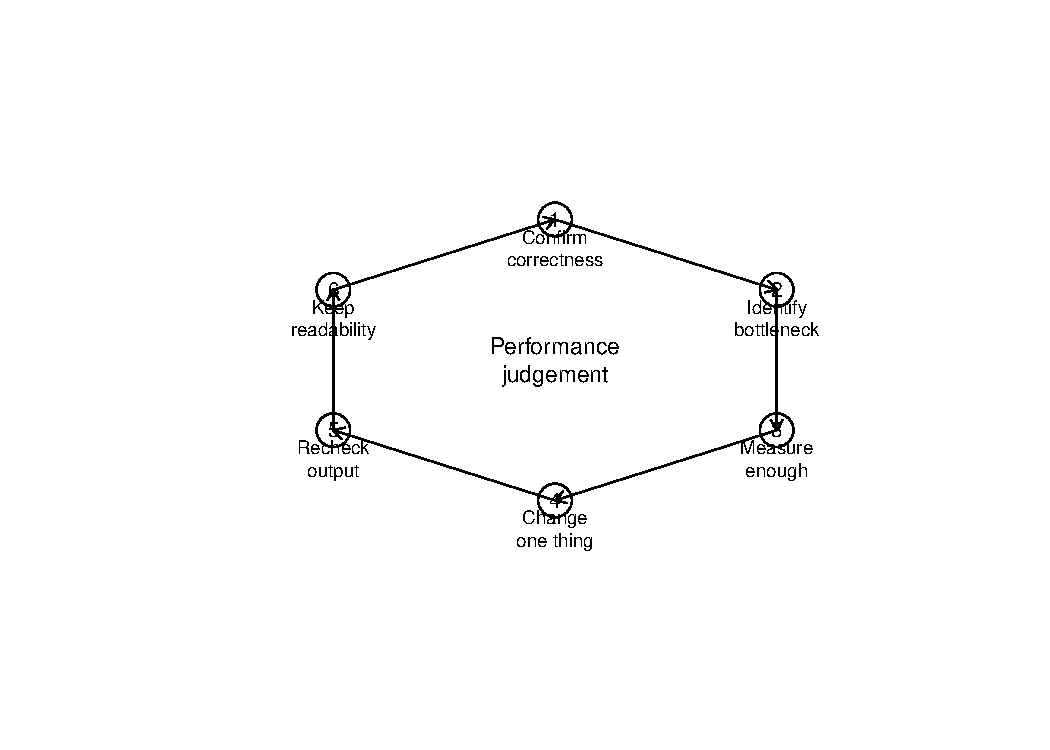
\includegraphics[width=0.9\linewidth,height=\textheight,keepaspectratio,alt={A circular workflow showing six steps: confirm correctness, identify bottleneck, measure enough, change one thing, recheck output, keep readability.}]{chapters/24-performance-and-scale_files/figure-pdf/fig-24-performance-cycle-1.pdf}

}

\caption{\label{fig-24-performance-cycle}A Disciplined Cycle for
Improving Performance Without Losing Trust.}

\end{figure}%

The cycle in Figure~\ref{fig-24-performance-cycle} protects Leo from two
opposite errors. The first is doing nothing while the workflow becomes
painful. The second is rewriting everything without knowing what problem
he is solving.

This cycle also connects directly to
\hyperref[reliability-and-automation-making-workflows-repeatable]{Chapter
23}. A reliable workflow gives Leo something stable to measure. Without
stability, performance work becomes guesswork.

\section{A Small Applied Example Using the Learner
Dataset}\label{a-small-applied-example-using-the-learner-dataset}

Now Leo can apply the performance lens to the learner dataset.

Suppose he wants a country-level summary of study behaviour and project
performance. The task is ordinary. That is the point. Performance
problems often begin in ordinary tasks repeated many times.

The following evaluated chunk uses base R so that the chapter remains
render-safe. If the project's \texttt{df\_analysis} file is available,
the setup chunk has already loaded it. Otherwise, the chapter uses a
small teaching fallback. Table~\ref{tbl-24-country-summary} shows the
resulting country-level summary.

\begin{Shaded}
\begin{Highlighting}[]
\NormalTok{required\_summary\_cols }\OtherTok{\textless{}{-}} \FunctionTok{c}\NormalTok{(}\StringTok{"country"}\NormalTok{, }\StringTok{"study\_hours"}\NormalTok{, }\StringTok{"project\_score"}\NormalTok{)}
\NormalTok{has\_required\_summary\_cols }\OtherTok{\textless{}{-}} \FunctionTok{all}\NormalTok{(required\_summary\_cols }\SpecialCharTok{\%in\%} \FunctionTok{names}\NormalTok{(df\_ch24))}

\ControlFlowTok{if}\NormalTok{ (has\_required\_summary\_cols) \{}
\NormalTok{  summary\_data }\OtherTok{\textless{}{-}} \FunctionTok{data.frame}\NormalTok{(}
    \AttributeTok{country =}\NormalTok{ df\_ch24}\SpecialCharTok{$}\NormalTok{country,}
    \AttributeTok{study\_hours =} \FunctionTok{suppressWarnings}\NormalTok{(}\FunctionTok{as.numeric}\NormalTok{(df\_ch24}\SpecialCharTok{$}\NormalTok{study\_hours)),}
    \AttributeTok{project\_score =} \FunctionTok{suppressWarnings}\NormalTok{(}\FunctionTok{as.numeric}\NormalTok{(df\_ch24}\SpecialCharTok{$}\NormalTok{project\_score)),}
    \AttributeTok{stringsAsFactors =} \ConstantTok{FALSE}
\NormalTok{  )}

\NormalTok{  country\_values }\OtherTok{\textless{}{-}} \FunctionTok{sort}\NormalTok{(}\FunctionTok{unique}\NormalTok{(summary\_data}\SpecialCharTok{$}\NormalTok{country[}\SpecialCharTok{!}\FunctionTok{is.na}\NormalTok{(summary\_data}\SpecialCharTok{$}\NormalTok{country)]))}

\NormalTok{  learners }\OtherTok{\textless{}{-}} \FunctionTok{as.integer}\NormalTok{(}\FunctionTok{table}\NormalTok{(}
    \FunctionTok{factor}\NormalTok{(summary\_data}\SpecialCharTok{$}\NormalTok{country, }\AttributeTok{levels =}\NormalTok{ country\_values)}
\NormalTok{  ))}

\NormalTok{  average\_study\_hours }\OtherTok{\textless{}{-}} \FunctionTok{round}\NormalTok{(}
    \FunctionTok{tapply}\NormalTok{(}
\NormalTok{      summary\_data}\SpecialCharTok{$}\NormalTok{study\_hours,}
\NormalTok{      summary\_data}\SpecialCharTok{$}\NormalTok{country,}
\NormalTok{      mean,}
      \AttributeTok{na.rm =} \ConstantTok{TRUE}
\NormalTok{    )[country\_values],}
    \DecValTok{2}
\NormalTok{  )}

\NormalTok{  average\_project\_score }\OtherTok{\textless{}{-}} \FunctionTok{round}\NormalTok{(}
    \FunctionTok{tapply}\NormalTok{(}
\NormalTok{      summary\_data}\SpecialCharTok{$}\NormalTok{project\_score,}
\NormalTok{      summary\_data}\SpecialCharTok{$}\NormalTok{country,}
\NormalTok{      mean,}
      \AttributeTok{na.rm =} \ConstantTok{TRUE}
\NormalTok{    )[country\_values],}
    \DecValTok{2}
\NormalTok{  )}

\NormalTok{  country\_summary }\OtherTok{\textless{}{-}} \FunctionTok{data.frame}\NormalTok{(}
    \AttributeTok{Country =}\NormalTok{ country\_values,}
    \AttributeTok{Learners =}\NormalTok{ learners,}
    \StringTok{\textasciigrave{}}\AttributeTok{Average study hours}\StringTok{\textasciigrave{}} \OtherTok{=} \FunctionTok{as.numeric}\NormalTok{(average\_study\_hours),}
    \StringTok{\textasciigrave{}}\AttributeTok{Average project score}\StringTok{\textasciigrave{}} \OtherTok{=} \FunctionTok{as.numeric}\NormalTok{(average\_project\_score),}
    \AttributeTok{check.names =} \ConstantTok{FALSE}
\NormalTok{  )}
\NormalTok{\} }\ControlFlowTok{else}\NormalTok{ \{}
\NormalTok{  country\_summary }\OtherTok{\textless{}{-}} \FunctionTok{data.frame}\NormalTok{(}
    \AttributeTok{Country =} \FunctionTok{character}\NormalTok{(),}
    \AttributeTok{Learners =} \FunctionTok{integer}\NormalTok{(),}
    \StringTok{\textasciigrave{}}\AttributeTok{Average study hours}\StringTok{\textasciigrave{}} \OtherTok{=} \FunctionTok{numeric}\NormalTok{(),}
    \StringTok{\textasciigrave{}}\AttributeTok{Average project score}\StringTok{\textasciigrave{}} \OtherTok{=} \FunctionTok{numeric}\NormalTok{(),}
    \AttributeTok{check.names =} \ConstantTok{FALSE}
\NormalTok{  )}
\NormalTok{\}}

\NormalTok{knitr}\SpecialCharTok{::}\FunctionTok{kable}\NormalTok{(country\_summary)}
\end{Highlighting}
\end{Shaded}

{

\begin{longtable}[]{@{}lrrr@{}}

\caption{\label{tbl-24-country-summary}A Country-Level Summary Created
Once and Reused Deliberately.}

\tabularnewline

\toprule\noalign{}
Country & Learners & Average study hours & Average project score \\
\midrule\noalign{}
\endhead
\bottomrule\noalign{}
\endlastfoot
Australia & 21 & 12.40 & 80.18 \\
Brazil & 18 & 12.01 & 76.51 \\
Canada & 31 & 11.29 & 77.65 \\
China & 28 & 12.78 & 80.97 \\
Denmark & 47 & 11.53 & 81.94 \\
France & 24 & 10.69 & 74.22 \\
Germany & 33 & 12.62 & 86.67 \\
India & 25 & 11.98 & 84.16 \\
Indonesia & 12 & 12.04 & 85.56 \\
Ireland & 42 & 11.26 & 84.09 \\
Japan & 25 & 12.13 & 78.76 \\
Mexico & 22 & 12.20 & 81.88 \\
Netherlands & 30 & 11.77 & 79.30 \\
Nigeria & 19 & 10.56 & 78.55 \\
Norway & 43 & 11.32 & 79.42 \\
Singapore & 44 & 12.79 & 80.65 \\
South Korea & 26 & 12.72 & 83.87 \\
Switzerland & 27 & 10.95 & 78.25 \\
United Kingdom & 34 & 11.29 & 81.11 \\
United States & 33 & 12.14 & 80.57 \\

\end{longtable}

}

The point of Table~\ref{tbl-24-country-summary} is not that base R is
always faster than every alternative. The point is that a meaningful
summary should be created once, named clearly, inspected, and reused. If
the same summary is needed in several places, Leo should not copy the
entire calculation into every report section.

That principle is simple. It has large consequences.

If a workflow needs the same summary for a table, a figure, and a
paragraph, the project can create \texttt{country\_summary} once and use
it three times. This improves speed, reduces drift, and makes the logic
easier to inspect.

\section{Reducing Repetition Without Hiding
Meaning}\label{reducing-repetition-without-hiding-meaning}

Repeated work is one of the easiest performance problems to miss. It
often appears as a normal habit: copy a chunk, change a variable, run
again. At first, this feels efficient. Later, it becomes expensive.

The correction is not to hide everything inside complicated
abstractions. The correction is to name repeated ideas at the right
level.

If Leo repeatedly calculates summary statistics for different groups, a
small helper function may be appropriate. If he repeatedly renders
reports for different audiences, a parameterised Quarto document may be
appropriate. If he repeatedly reads and cleans the same raw files, a
script route may be appropriate. If he repeatedly uses the same
project-specific functions, the package habits from
\hyperref[from-functions-to-packages-building-reusable-r-tools]{Chapter
22} become relevant.

Table~\ref{tbl-24-repetition-responses} shows the response that fits
each kind of repetition.

\begin{Shaded}
\begin{Highlighting}[]
\NormalTok{repetition\_responses }\OtherTok{\textless{}{-}} \FunctionTok{data.frame}\NormalTok{(}
  \AttributeTok{RepetitionType =} \FunctionTok{c}\NormalTok{(}
    \StringTok{"Same expression repeated inside one script"}\NormalTok{,}
    \StringTok{"Same transformation repeated across scripts"}\NormalTok{,}
    \StringTok{"Same report repeated for different groups"}\NormalTok{,}
    \StringTok{"Same cleaning route repeated for fresh data"}\NormalTok{,}
    \StringTok{"Same project tools reused across projects"}
\NormalTok{  ),}
  \AttributeTok{BetterResponse =} \FunctionTok{c}\NormalTok{(}
    \StringTok{"Create a named object or small helper function"}\NormalTok{,}
    \StringTok{"Move the logic into one script or reusable function"}\NormalTok{,}
    \StringTok{"Use parameters or a controlled rendering strategy"}\NormalTok{,}
    \StringTok{"Automate the import{-}clean{-}prepare route with checks"}\NormalTok{,}
    \StringTok{"Organise the tools into package{-}like structure"}
\NormalTok{  ),}
  \AttributeTok{PerformanceBenefit =} \FunctionTok{c}\NormalTok{(}
    \StringTok{"Avoids recalculating or rewriting the same logic"}\NormalTok{,}
    \StringTok{"Reduces drift and repeated computation"}\NormalTok{,}
    \StringTok{"Prevents manual copy{-}paste report production"}\NormalTok{,}
    \StringTok{"Makes repeated updates more efficient and reliable"}\NormalTok{,}
    \StringTok{"Turns repeated project knowledge into reusable tools"}
\NormalTok{  ),}
  \AttributeTok{Continuity =} \FunctionTok{c}\NormalTok{(}
    \StringTok{"Functions from earlier chapters"}\NormalTok{,}
    \StringTok{"Workflow discipline from Chapter 23"}\NormalTok{,}
    \StringTok{"Quarto reporting from Part 5"}\NormalTok{,}
    \StringTok{"Reliability and automation from Chapter 23"}\NormalTok{,}
    \StringTok{"Reusable tool organisation from Chapter 22"}
\NormalTok{  ),}
  \AttributeTok{check.names =} \ConstantTok{FALSE}
\NormalTok{)}

\NormalTok{knitr}\SpecialCharTok{::}\FunctionTok{kable}\NormalTok{(repetition\_responses)}
\end{Highlighting}
\end{Shaded}

{

\begin{longtable}[]{@{}
  >{\raggedright\arraybackslash}p{(\linewidth - 6\tabcolsep) * \real{0.2292}}
  >{\raggedright\arraybackslash}p{(\linewidth - 6\tabcolsep) * \real{0.2708}}
  >{\raggedright\arraybackslash}p{(\linewidth - 6\tabcolsep) * \real{0.2760}}
  >{\raggedright\arraybackslash}p{(\linewidth - 6\tabcolsep) * \real{0.2240}}@{}}

\caption{\label{tbl-24-repetition-responses}Matching Different Forms of
Repetition to Appropriate Workflow Responses.}

\tabularnewline

\toprule\noalign{}
\begin{minipage}[b]{\linewidth}\raggedright
RepetitionType
\end{minipage} & \begin{minipage}[b]{\linewidth}\raggedright
BetterResponse
\end{minipage} & \begin{minipage}[b]{\linewidth}\raggedright
PerformanceBenefit
\end{minipage} & \begin{minipage}[b]{\linewidth}\raggedright
Continuity
\end{minipage} \\
\midrule\noalign{}
\endhead
\bottomrule\noalign{}
\endlastfoot
Same expression repeated inside one script & Create a named object or
small helper function & Avoids recalculating or rewriting the same logic
& Functions from earlier chapters \\
Same transformation repeated across scripts & Move the logic into one
script or reusable function & Reduces drift and repeated computation &
Workflow discipline from Chapter 23 \\
Same report repeated for different groups & Use parameters or a
controlled rendering strategy & Prevents manual copy-paste report
production & Quarto reporting from Part 5 \\
Same cleaning route repeated for fresh data & Automate the
import-clean-prepare route with checks & Makes repeated updates more
efficient and reliable & Reliability and automation from Chapter 23 \\
Same project tools reused across projects & Organise the tools into
package-like structure & Turns repeated project knowledge into reusable
tools & Reusable tool organisation from Chapter 22 \\

\end{longtable}

}

The most important word in Table~\ref{tbl-24-repetition-responses} is
``appropriate.'' Not every repeated line deserves a function. Not every
function deserves a package. Not every report deserves a parameterised
system. Performance work should reduce friction without creating
unnecessary machinery.

\section{Common Mistakes Leo Should
Avoid}\label{common-mistakes-leo-should-avoid}

Performance work attracts mistakes because it feels technical. The
common errors are not only coding errors. They are judgement errors.

Table~\ref{tbl-24-common-mistakes} names the most important ones.

\begin{Shaded}
\begin{Highlighting}[]
\NormalTok{common\_mistakes }\OtherTok{\textless{}{-}} \FunctionTok{data.frame}\NormalTok{(}
  \AttributeTok{Mistake =} \FunctionTok{c}\NormalTok{(}
    \StringTok{"Optimising before checking correctness"}\NormalTok{,}
    \StringTok{"Assuming the visible line is the bottleneck"}\NormalTok{,}
    \StringTok{"Replacing clear code with clever code too early"}\NormalTok{,}
    \StringTok{"Benchmarking tiny examples and overgeneralising"}\NormalTok{,}
    \StringTok{"Loading advanced packages without a real need"}\NormalTok{,}
    \StringTok{"Repeating expensive work across chunks"}\NormalTok{,}
    \StringTok{"Assuming more cores always means faster work"}\NormalTok{,}
    \StringTok{"Keeping every intermediate object forever"}
\NormalTok{  ),}
  \AttributeTok{WhyItHurts =} \FunctionTok{c}\NormalTok{(}
    \StringTok{"The project may preserve a wrong result more efficiently"}\NormalTok{,}
    \StringTok{"Time is spent changing code that does not limit the workflow"}\NormalTok{,}
    \StringTok{"The project becomes harder to audit and maintain"}\NormalTok{,}
    \StringTok{"Small examples may not represent the actual workflow"}\NormalTok{,}
    \StringTok{"Dependency weight increases without solving the problem"}\NormalTok{,}
    \StringTok{"Render time grows as the report expands"}\NormalTok{,}
    \StringTok{"Parallel overhead and memory pressure may make the workflow slower or less stable"}\NormalTok{,}
    \StringTok{"Memory and interpretation both become heavier"}
\NormalTok{  ),}
  \AttributeTok{BetterHabit =} \FunctionTok{c}\NormalTok{(}
    \StringTok{"Validate first, then optimise"}\NormalTok{,}
    \StringTok{"Measure enough to locate the bottleneck"}\NormalTok{,}
    \StringTok{"Prefer readable efficiency"}\NormalTok{,}
    \StringTok{"Use timing as evidence, not as a universal law"}\NormalTok{,}
    \StringTok{"Escalate tools only when the project justifies them"}\NormalTok{,}
    \StringTok{"Create once, name clearly, reuse deliberately"}\NormalTok{,}
    \StringTok{"Use parallel workers only when the task is independent and worth the overhead"}\NormalTok{,}
    \StringTok{"Keep meaningful stages, remove temporary clutter"}
\NormalTok{  ),}
  \AttributeTok{check.names =} \ConstantTok{FALSE}
\NormalTok{)}

\NormalTok{knitr}\SpecialCharTok{::}\FunctionTok{kable}\NormalTok{(common\_mistakes)}
\end{Highlighting}
\end{Shaded}

{

\begin{longtable}[]{@{}
  >{\raggedright\arraybackslash}p{(\linewidth - 4\tabcolsep) * \real{0.2308}}
  >{\raggedright\arraybackslash}p{(\linewidth - 4\tabcolsep) * \real{0.3942}}
  >{\raggedright\arraybackslash}p{(\linewidth - 4\tabcolsep) * \real{0.3750}}@{}}

\caption{\label{tbl-24-common-mistakes}Common Beginner Mistakes When
Trying to Improve R Performance.}

\tabularnewline

\toprule\noalign{}
\begin{minipage}[b]{\linewidth}\raggedright
Mistake
\end{minipage} & \begin{minipage}[b]{\linewidth}\raggedright
WhyItHurts
\end{minipage} & \begin{minipage}[b]{\linewidth}\raggedright
BetterHabit
\end{minipage} \\
\midrule\noalign{}
\endhead
\bottomrule\noalign{}
\endlastfoot
Optimising before checking correctness & The project may preserve a
wrong result more efficiently & Validate first, then optimise \\
Assuming the visible line is the bottleneck & Time is spent changing
code that does not limit the workflow & Measure enough to locate the
bottleneck \\
Replacing clear code with clever code too early & The project becomes
harder to audit and maintain & Prefer readable efficiency \\
Benchmarking tiny examples and overgeneralising & Small examples may not
represent the actual workflow & Use timing as evidence, not as a
universal law \\
Loading advanced packages without a real need & Dependency weight
increases without solving the problem & Escalate tools only when the
project justifies them \\
Repeating expensive work across chunks & Render time grows as the report
expands & Create once, name clearly, reuse deliberately \\
Assuming more cores always means faster work & Parallel overhead and
memory pressure may make the workflow slower or less stable & Use
parallel workers only when the task is independent and worth the
overhead \\
Keeping every intermediate object forever & Memory and interpretation
both become heavier & Keep meaningful stages, remove temporary
clutter \\

\end{longtable}

}

The mistakes in Table~\ref{tbl-24-common-mistakes} are common because
they feel productive. Leo may feel as if he is improving the project
when he adds a faster package, rewrites a pipeline, or removes
intermediate objects. But the professional test is stricter: did the
change solve the real problem without damaging trust?

\section{Try It Yourself}\label{try-it-yourself-8}

Choose one script or chapter from your current project and inspect it
through the performance lens.

Do not change anything at first. Read it and answer these questions:

\begin{enumerate}
\def\labelenumi{\arabic{enumi}.}
\tightlist
\item
  Which parts are repeated?
\item
  Which objects are created but never used again?
\item
  Which chunks recreate the same summary?
\item
  Which imports happen more than once?
\item
  Which operations would become uncomfortable if the data had ten times
  more rows?
\item
  Which parts must remain clear even if they could be written more
  compactly?
\end{enumerate}

Then make only one improvement.

Do not rewrite the whole project. Choose one meaningful change: remove
one repeated calculation, create one reusable object, select only needed
columns for one task, or add one simple timing check around a suspicious
section.

After the change, rerun the relevant output and confirm that the result
still means the same thing.

\section{A Small Practice Lab}\label{a-small-practice-lab-11}

Listing~\ref{lst-24-practice-lab} gives Leo a practical scaffold. It is
not evaluated because the point is for him to apply it inside his own
project, where the real bottlenecks live.

\begin{codelisting}

\caption{\label{lst-24-practice-lab}A Practice-Lab Scaffold for
Diagnosing Performance and Scale in a Real Project.}

\centering{

\begin{Shaded}
\begin{Highlighting}[]
\CommentTok{\# Practice Lab: Make one workflow lighter}

\CommentTok{\# 1. Pick one script, report, or chapter that feels slow or heavy.}

\CommentTok{\# 2. Confirm correctness first:}
\CommentTok{\#    {-} Does the current output look right?}
\CommentTok{\#    {-} Are missing values handled deliberately?}
\CommentTok{\#    {-} Are the important summaries stable after rerunning?}

\CommentTok{\# 3. Identify one suspected bottleneck:}
\CommentTok{\#    {-} repeated import}
\CommentTok{\#    {-} repeated summary}
\CommentTok{\#    {-} unnecessary columns}
\CommentTok{\#    {-} row{-}by{-}row logic}
\CommentTok{\#    {-} large temporary objects}
\CommentTok{\#    {-} expensive chunk during render}

\CommentTok{\# 4. Measure enough to avoid guessing:}
\CommentTok{\#    system.time(\{}
\CommentTok{\#      \# place the suspected operation here}
\CommentTok{\#    \})}

\CommentTok{\# 5. Make one change:}
\CommentTok{\#    {-} reuse a named summary}
\CommentTok{\#    {-} select needed columns}
\CommentTok{\#    {-} replace row{-}by{-}row code with vectorised code}
\CommentTok{\#    {-} move repeated logic into a function}
\CommentTok{\#    {-} avoid recalculating the same result in many chunks}

\CommentTok{\# 6. Recheck the output:}
\CommentTok{\#    {-} Did the result stay the same?}
\CommentTok{\#    {-} Is the code still readable?}
\CommentTok{\#    {-} Did the change improve the workflow enough to keep?}

\CommentTok{\# 7. Write a short note:}
\CommentTok{\#    {-} What was changed?}
\CommentTok{\#    {-} Why was it changed?}
\CommentTok{\#    {-} What should a future reader know?}
\end{Highlighting}
\end{Shaded}

}

\end{codelisting}%

The lab in Listing~\ref{lst-24-practice-lab} teaches a disciplined
habit: improve the project where the project asks to be improved.
Performance work should respond to evidence.

\section{Short Recap}\label{short-recap-10}

Leo began this chapter with a script that worked but no longer felt
light. That situation is normal. As data, reports, and repeated requests
grow, a correct workflow may begin to feel slow, heavy, or difficult to
scale.

He learned that performance is not a race to make every line faster. It
is a form of judgement. The first task is to protect correctness. The
second is to preserve repeatability. Only then should Leo identify the
actual bottleneck and improve the smallest meaningful part of the
workflow.

He learned that scale can mean more rows, more columns, more groups,
more files, more outputs, more collaborators, or more frequent rebuilds.
He also learned that timing tools are useful but limited. They help him
diagnose; they do not replace judgement.

He saw why vectorised thinking matters in R, why small examples can
mislead, why memory and object size deserve attention, and why efficient
pipelines should remain readable. He also learned that \texttt{apply},
\texttt{purrr}, and \texttt{foreach} serve different purposes, and that
parallel computing is useful only when independent work is large enough
to justify the overhead. Optional tools such as \texttt{data.table},
databases, Arrow-style workflows, and parallel backends are
possibilities for later growth, not requirements for every project.

Most importantly, Leo learned that performance is part of workflow
design. A professional project should not merely run once. It should run
again, remain understandable, and avoid unnecessary friction as the work
expands.

\section{Leo's Notebook}\label{leos-notebook-13}

\begin{itemize}
\tightlist
\item
  Correctness comes before speed.
\item
  A repeatable workflow is easier to measure than a fragile one.
\item
  ``R is slow'' is not a diagnosis. Find the bottleneck.
\item
  Performance problems may come from time, memory, repetition, imports,
  outputs, or workflow design.
\item
  Vectorised code often fits R better than row-by-row thinking.
\item
  A small inefficiency becomes important when it is repeated many times.
\item
  Do not trust a faster rewrite until the output has been checked.
\item
  \texttt{apply} and \texttt{purrr} organise repetition; they do not
  guarantee speed by themselves.
\item
  Parallel computing is useful only when independent tasks are large
  enough to justify worker setup and coordination.
\item
  Optional performance tools are useful only when the problem justifies
  their cost.
\item
  Readability is part of performance because future work must still be
  possible.
\item
  The best performance change is often small, specific, measured, and
  documented.
\end{itemize}

\section{Glossary}\label{glossary-10}

\textbf{Bottleneck}\\
The part of a workflow that limits the speed, responsiveness, memory
use, or maintainability of the whole project.

\textbf{Core}\\
A processing unit that can carry out computation. Many computers have
multiple cores, but ordinary R code does not automatically distribute
every task across all of them.

\textbf{Worker}\\
A separate R process used in parallel computing to handle one part of a
divided task. Workers can reduce elapsed time for suitable tasks, but
they also require setup, memory, and coordination.

\textbf{Memory}\\
The working space R uses to hold objects during a session. Large objects
and unnecessary copies can increase memory pressure.

\textbf{Object size}\\
The approximate amount of memory used by an R object. It can be
inspected with \texttt{object.size()}.

\textbf{Performance}\\
The practical behaviour of code or a workflow in relation to time,
memory, repetition, and responsiveness.

\textbf{Premature optimisation}\\
Changing code for speed before confirming correctness, repeatability, or
the real bottleneck.

\textbf{Parallel computing}\\
Running independent pieces of work at the same time through multiple
worker processes or cores, usually with extra setup, memory, and
coordination costs.

\textbf{Repetition tool}\\
A function or pattern, such as \texttt{lapply()}, \texttt{purrr::map()},
or \texttt{foreach()}, that helps express repeated work more
systematically.

\textbf{Scale}\\
The point at which a workflow must handle more rows, columns, groups,
files, outputs, collaborators, or repeated rebuilds than before.

\textbf{Timing}\\
Measuring how long code takes to run. In base R, \texttt{system.time()}
provides a simple first timing tool.

\textbf{Vectorisation}\\
Writing code so that R operates on whole vectors rather than manually
processing one value at a time in user-written row-by-row logic.

\textbf{Workflow design}\\
The deliberate organisation of inputs, scripts, objects, outputs,
checks, and repeated actions so that a project remains clear and
workable as it grows.

\section{Chapter Outcome}\label{chapter-outcome-23}

By the end of this chapter, Leo can explain why performance should come
after correctness and reliability. He can distinguish speed, memory,
repetition, and workflow friction. He can use a simple timing pattern to
investigate a suspected bottleneck. He understands why vectorised
operations often fit R better than row-by-row thinking, and he knows
that object size and unnecessary copies can matter as projects grow.

He can also make tool choices more carefully. He knows that base R and
tidyverse workflows are often enough, that \texttt{apply}-style tools
organise repetition rather than automatically reducing time, and that
optional tools such as \texttt{data.table}, databases, Arrow-style
workflows, \texttt{foreach}, and parallel backends have specific use
cases. New packages and new execution models should not be added merely
because they sound advanced.

Most importantly, Leo can now ask a stronger professional question:

\begin{quote}
Can this workflow stay clear, correct, repeatable, and efficient as the
work grows?
\end{quote}

That question completes the final technical discipline before
integration.

\section{What Comes Next}\label{what-comes-next-12}

Leo now has the last missing habit before the book's final project.

He can write code. He can debug it. He can import, clean, transform,
summarise, visualise, and communicate data. He can build reproducible
reports, connect data sources, collaborate through traceable changes,
organise reusable tools, make workflows repeatable, and now think about
performance and scale.

The remaining task is not another isolated skill. It is integration.

\href{25-final-integration-project.qmd}{Chapter 25} brings the pieces
together. It asks Leo to stop seeing the book as separate lessons and
start seeing the full analytical route as one connected system: data
input, cleaning, transformation, analysis, visualisation, reporting,
reliability, automation, performance, and final delivery.

Chapter 24 has asked whether a repeatable workflow can remain efficient
as the work grows. Chapter 25 asks whether all the parts can now become
one professional analytical product.

\chapter{Final Integration Project: Building an End-to-End Analytical
System}\label{final-integration-project-building-an-end-to-end-analytical-system}

\renewcommand{\thefigure}{25.\arabic{figure}}  
\setcounter{figure}{0}

\renewcommand{\thetable}{25.\arabic{table}}  
\setcounter{table}{0}

\section{Opening Scene: The Last Question Is Not a
Command}\label{opening-scene-the-last-question-is-not-a-command}

Leo reaches the final chapter with a different kind of problem.

At the beginning of the book, his question was small and urgent:
\emph{How do I make R do this one thing?} He wanted the command that
would import a file, clean a column, draw a plot, calculate a summary,
or render a report. That was a reasonable place to begin. A learner
cannot build a system before he trusts the first brick.

Now the question has changed.

Leo no longer wants one command. He wants a complete piece of work that
another person can open, inspect, rerun, and trust. He wants the raw
learner data to enter the project through a clear path. He wants the
cleaning choices to be visible. He wants the analysis-ready object to be
created in a known place. He wants the summaries and figures to match
the report. He wants the report to rebuild without private memory,
manual clicking, or hidden corrections. He wants the project to survive
revision.

This is the final professional threshold.

A script can work once and still not be a system. A report can look
polished and still be fragile. A project can contain good code and still
fail because the parts are not connected.

In \hyperref[performance-and-scale-making-r-work-efficiently]{Chapter
24}, Leo learned that efficient work is not the same as making every
line faster. Performance is practical judgement. Scale is about knowing
when time, memory, repeated work, file movement, and machine resources
matter. Chapter 25 adds the last discipline: integration.

Leo now has to prove that the whole project can stand.

\section{The Final Lightbulb Idea}\label{the-final-lightbulb-idea}

\begin{tcolorbox}[enhanced jigsaw, arc=.35mm, bottomrule=.15mm, bottomtitle=1mm, breakable, colback=white, colbacktitle=quarto-callout-tip-color!10!white, colframe=quarto-callout-tip-color-frame, coltitle=black, left=2mm, leftrule=.75mm, opacityback=0, opacitybacktitle=0.6, rightrule=.15mm, title=\textcolor{quarto-callout-tip-color}{\faLightbulb}\hspace{0.5em}{The final lightbulb idea}, titlerule=0mm, toprule=.15mm, toptitle=1mm]

An analytical system is not a collection of scripts. It is a connected
workflow where data, code, checks, outputs, and explanation rebuild
together.

\end{tcolorbox}

That sentence changes the meaning of the final project. Leo is not being
asked to remember everything from the book. He is being asked to connect
the parts into one working route.

The route matters because professional analysis is not only judged by
the answer. It is judged by how the answer was produced, whether it can
be inspected, whether it can be rerun, and whether the next person can
understand what changed.

Chapter 25 therefore does not introduce a new trick. It integrates what
Leo has already built.

\section{Why Integration Is the Last
Skill}\label{why-integration-is-the-last-skill}

Integration belongs at the end because it depends on everything before
it. Leo cannot integrate a workflow he does not understand. He cannot
connect cleaning, transformation, reporting, version control,
automation, and performance if each of those remains a disconnected
memory.

Earlier chapters gave Leo the working parts. Part 5 then moved him from
reports into systems.
\hyperref[reproducible-reports-with-quarto-turning-analysis-into-a-document]{Chapter
19} made analysis communicable through Quarto.
\hyperref[data-connections-moving-beyond-local-files]{Chapter 20}
expanded Leo's sense of where data can come from.
\hyperref[collaboration-and-version-control-making-work-traceable]{Chapter
21} made change traceable.
\hyperref[from-functions-to-packages-building-reusable-r-tools]{Chapter
22} showed that reusable actions can be organised into reusable tools.
\hyperref[reliability-and-automation-making-workflows-repeatable]{Chapter
23} taught Leo to rebuild work through reliable checks and repeatable
execution.
\hyperref[performance-and-scale-making-r-work-efficiently]{Chapter 24}
taught him to think about efficiency without worshipping speed.

Now those skills have to operate together.

This chapter is not a summary of Chapters 1 to 24. A summary would list
what Leo has learned. A capstone asks whether he can use those skills
together under realistic conditions. The final task is no longer, ``Can
Leo run this code?'' The better question is, ``Can Leo build a project
where the route from evidence to explanation is visible?''

\begin{tcolorbox}[enhanced jigsaw, arc=.35mm, bottomrule=.15mm, bottomtitle=1mm, breakable, colback=white, colbacktitle=quarto-callout-note-color!10!white, colframe=quarto-callout-note-color-frame, coltitle=black, left=2mm, leftrule=.75mm, opacityback=0, opacitybacktitle=0.6, rightrule=.15mm, title=\textcolor{quarto-callout-note-color}{\faInfo}\hspace{0.5em}{What this chapter is doing}, titlerule=0mm, toprule=.15mm, toptitle=1mm]

This chapter integrates rather than introduces. It gives Leo a final
guided project that uses the book's official learner dataset and the
objects that emanate from it. The purpose is not to add a new advanced
tool. The purpose is to assemble a trustworthy analytical system.

\end{tcolorbox}

Table~\ref{tbl-25-final-workflow-map} maps the final project stages to
the earlier skills Leo is now joining into one route.

{

\begin{longtable}[]{@{}
  >{\raggedright\arraybackslash}p{(\linewidth - 4\tabcolsep) * \real{0.1958}}
  >{\raggedright\arraybackslash}p{(\linewidth - 4\tabcolsep) * \real{0.4762}}
  >{\raggedright\arraybackslash}p{(\linewidth - 4\tabcolsep) * \real{0.3280}}@{}}

\caption{\label{tbl-25-final-workflow-map}Final Integration Workflow Map
for the End-to-End Analytical System.}

\tabularnewline

\toprule\noalign{}
\begin{minipage}[b]{\linewidth}\raggedright
Project stage
\end{minipage} & \begin{minipage}[b]{\linewidth}\raggedright
What Leo is doing
\end{minipage} & \begin{minipage}[b]{\linewidth}\raggedright
Earlier skill now being integrated
\end{minipage} \\
\midrule\noalign{}
\endhead
\bottomrule\noalign{}
\endlastfoot
Define the analytical question & Converts curiosity into a bounded
analytical task. & Problem framing and analytical judgement \\
Prepare the project environment & Confirms packages, folders, paths, and
project assumptions. & Packages, projects, paths, and reproducibility \\
Import the raw learner data & Reads \texttt{df\_r\_migration\_messy.csv}
through an explicit project-relative route. & Importing data \\
Inspect the imported object & Checks names, dimensions, types, and
obvious irregularities before cleaning. & Inspection before
interpretation \\
Clean and prepare the evidence & Standardises names, types, missing
values, dates, categories, and obvious data issues. & Cleaning and
preparing data \\
Create the analysis-ready object & Produces \texttt{df\_analysis} as the
stable object for final summaries and figures. & Selecting, filtering,
transforming, summarising, and grouping \\
Validate assumptions and outputs & Checks row counts, required columns,
plausible ranges, and output consistency. & Debugging, reliability, and
automation \\
Summarise learner patterns & Creates tables that answer the final
question without hiding the method. & Summarising evidence \\
Visualise key relationships & Creates figures that communicate patterns
rather than decorate the report. & Data visualisation and
communication \\
Render the Quarto report & Combines code, output, and explanation in one
reproducible document. & Reproducible reporting with Quarto \\
Preserve the project history & Uses Git and clear commits so changes
remain visible and reversible. & Collaboration and version control \\
Review performance and scale & Keeps the final system efficient enough
to rebuild without unnecessary friction. & Performance and scale \\
Reflect on limits and next decisions & States what the evidence
suggests, what it cannot prove, and what should be checked next. &
Professional interpretation \\

\end{longtable}

}

The table is not a memory test. It is a coordination map. Leo is now
learning to see the workflow as one connected system rather than many
separate lessons.

\section{The Final Project Brief}\label{the-final-project-brief}

The final project uses the book's learner/R-migration dataset. The raw
file is the deliberately imperfect dataset:

\texttt{data/raw/df\_r\_migration\_messy.csv}

The central analysis-ready object is:

\texttt{df\_analysis}

The stable saved outputs should live in:

\texttt{data/processed/df\_analysis.rds}

and, where useful for sharing outside R:

\texttt{data/processed/df\_analysis.csv}

The final report should answer this bounded question:

\begin{quote}
What factors appear to support a learner's movement from R beginner to
confident, project-ready analyst?
\end{quote}

This question is deliberately practical. It does not pretend that the
dataset can prove every cause. It asks Leo to use the evidence
responsibly. He can examine relationships among study hours, completed
lessons, project scores, confidence, completion status, tool use, and
other fields available in the final analysis-ready dataset.

The final deliverable is not only a table or a plot. It is a complete
project route:

raw data → import → inspect → clean → transform → validate → summarise →
visualise → report → preserve → review.

The word \emph{appear} is important. It protects the analysis from
overclaiming. Leo can identify patterns. He can discuss plausible
support factors. He can show that learners with more completed lessons,
higher study engagement, stronger confidence, or more complete project
work tend to look more project-ready if the data support that pattern.
He cannot turn a teaching dataset into causal proof without a design
that supports causal inference.

That is not a weakness. It is analytical honesty.

\section{The Project Folder
Structure}\label{the-project-folder-structure}

A final project needs visible architecture. The structure does not need
to be complicated, but it must be honest. Files should not float around
the desktop. Scripts should not live inside the downloads folder.
Reports should not depend on hidden objects that only exist because Leo
ran something yesterday.

Table~\ref{tbl-25-project-files} shows the recommended structure for the
final project. It is intentionally modest. Leo does not need production
infrastructure to do professional work. He needs a clear route.

{

\begin{longtable}[]{@{}
  >{\raggedright\arraybackslash}p{(\linewidth - 6\tabcolsep) * \real{0.1833}}
  >{\raggedright\arraybackslash}p{(\linewidth - 6\tabcolsep) * \real{0.3542}}
  >{\raggedright\arraybackslash}p{(\linewidth - 6\tabcolsep) * \real{0.1042}}
  >{\raggedright\arraybackslash}p{(\linewidth - 6\tabcolsep) * \real{0.3583}}@{}}

\caption{\label{tbl-25-project-files}Recommended Final Project Structure
for the Chapter 25 Integration Project.}

\tabularnewline

\toprule\noalign{}
\begin{minipage}[b]{\linewidth}\raggedright
Folder or file
\end{minipage} & \begin{minipage}[b]{\linewidth}\raggedright
Purpose
\end{minipage} & \begin{minipage}[b]{\linewidth}\raggedright
Kind of project material
\end{minipage} & \begin{minipage}[b]{\linewidth}\raggedright
Leo should usually track it with Git?
\end{minipage} \\
\midrule\noalign{}
\endhead
\bottomrule\noalign{}
\endlastfoot
\texttt{data/raw/} & Stores untouched source data. & Source-data
location & Yes, as a folder placeholder if needed. \\
\texttt{data/raw/df\_r\_migration\_messy.csv} & The official raw learner
dataset used by the project. & Source data & Usually yes for this
teaching project because it is the distributed practice dataset. \\
\texttt{data/processed/} & Stores stable data objects created by the
workflow. & Processed-data location & Yes, as a folder placeholder if
needed. \\
\texttt{data/processed/df\_analysis.rds} & The primary analysis-ready R
object used by reports and scripts. & Processed data & Usually yes if
small and intentionally distributed with the teaching project. \\
\texttt{data/processed/df\_analysis.csv} & A shareable CSV version of
the analysis-ready dataset. & Processed data & Usually yes if small and
intentionally distributed with the teaching project. \\
\texttt{scripts/00\_setup\_env.R} & Prepares packages, folders, and
project assumptions. & Workflow script & Yes. \\
\texttt{scripts/01\_import\_data.R} & Imports raw data through a
project-relative path. & Workflow script & Yes. \\
\texttt{scripts/02\_clean\_data.R} & Cleans names, types, missing
values, categories, dates, and obvious inconsistencies. & Workflow
script & Yes. \\
\texttt{scripts/03\_create\_analysis\_data.R} & Creates the final
\texttt{df\_analysis} object used for summaries and figures. & Workflow
script & Yes. \\
\texttt{scripts/04\_validate\_outputs.R} & Checks required columns, row
counts, plausible values, and expected outputs. & Workflow script &
Yes. \\
\texttt{reports/final-integration-report.qmd} & Combines narrative,
code, tables, figures, and interpretation. & Report source & Yes. \\
\texttt{outputs/tables/} & Stores exported tables when the project needs
them outside the report. & Output location & Yes, if exported tables are
part of the project product. \\
\texttt{outputs/figures/} & Stores exported figures when the project
needs them outside the report. & Output location & Yes, if exported
figures are part of the project product. \\
\texttt{renv.lock} & Records package versions for environment
consistency. & Environment record & Yes. \\
\texttt{README.md} & Explains how to rebuild and understand the project.
& Documentation & Yes. \\
\texttt{chapters/25-final-integration-project.qmd} & Contains the final
capstone chapter in the Quarto book. & Book chapter source & Yes. \\

\end{longtable}

}

The same structure appears as a listing in
Listing~\ref{lst-25-project-structure}. The table explains the purpose.
The listing gives Leo a copyable mental picture of the project.

\begin{codelisting}

\caption{\label{lst-25-project-structure}A Final Project Folder
Structure for an End-to-End Analytical System.}

\centering{

\begin{Shaded}
\begin{Highlighting}[]
\ExtensionTok{not{-}so{-}short{-}introduction{-}to{-}r{-}renderable/}
\ExtensionTok{├──}\NormalTok{ data/}
\ExtensionTok{│}\NormalTok{   ├── raw/}
\ExtensionTok{│}\NormalTok{   │   └── df\_r\_migration\_messy.csv}
\ExtensionTok{│}\NormalTok{   └── processed/}
\ExtensionTok{│}\NormalTok{       ├── df\_analysis.rds}
\ExtensionTok{│}\NormalTok{       └── df\_analysis.csv}
\ExtensionTok{├──}\NormalTok{ scripts/}
\ExtensionTok{│}\NormalTok{   ├── 00\_setup\_env.R}
\ExtensionTok{│}\NormalTok{   ├── 01\_import\_data.R}
\ExtensionTok{│}\NormalTok{   ├── 02\_clean\_data.R}
\ExtensionTok{│}\NormalTok{   ├── 03\_create\_analysis\_data.R}
\ExtensionTok{│}\NormalTok{   └── 04\_validate\_outputs.R}
\ExtensionTok{├──}\NormalTok{ reports/}
\ExtensionTok{│}\NormalTok{   └── final{-}integration{-}report.qmd}
\ExtensionTok{├──}\NormalTok{ outputs/}
\ExtensionTok{│}\NormalTok{   ├── figures/}
\ExtensionTok{│}\NormalTok{   └── tables/}
\ExtensionTok{├──}\NormalTok{ chapters/}
\ExtensionTok{│}\NormalTok{   └── 25{-}final{-}integration{-}project.qmd}
\ExtensionTok{├──}\NormalTok{ renv.lock}
\ExtensionTok{├──}\NormalTok{ README.md}
\ExtensionTok{└──}\NormalTok{ \_quarto.yml}
\end{Highlighting}
\end{Shaded}

}

\end{codelisting}%

The folder structure is not decoration. It is a contract. Every part of
the project has a place, and every place has a purpose.

\section{The End-to-End Workflow Map}\label{the-end-to-end-workflow-map}

A final system needs more than folders. It needs movement.

Figure~\ref{fig-25-end-to-end-system} gives Leo the full route from raw
data to preserved work. The figure is deliberately plain because the
point is not graphic design. The point is to see the system as a
sequence of linked responsibilities.

\begin{figure}

\centering{

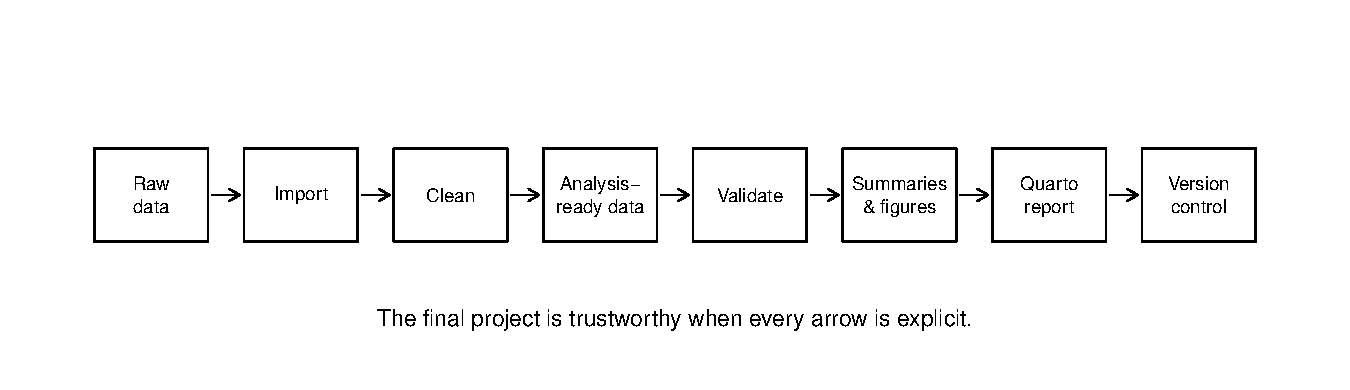
\includegraphics[width=0.9\linewidth,height=\textheight,keepaspectratio,alt={A left-to-right workflow diagram showing raw data moving through import, cleaning, analysis-ready data, validation, summaries and figures, Quarto report, and version control.}]{chapters/25-final-integration-project_files/figure-pdf/fig-25-end-to-end-system-1.pdf}

}

\caption{\label{fig-25-end-to-end-system}An End-to-End Analytical System
from Raw Data to Preserved Work.}

\end{figure}%

A broken system usually fails at the arrows. The data exists, but the
import path is unclear. The cleaning script exists, but the report does
not call it. The figure exists, but no one knows which dataset created
it. The report exists, but the package versions have shifted.
Integration is the discipline of protecting the arrows.

Figure~\ref{fig-25-final-output-flow} shows the same idea from the
output side. It reminds Leo that final tables, figures, and reports
should not be manually detached from the scripts that produce them.

\begin{figure}

\centering{

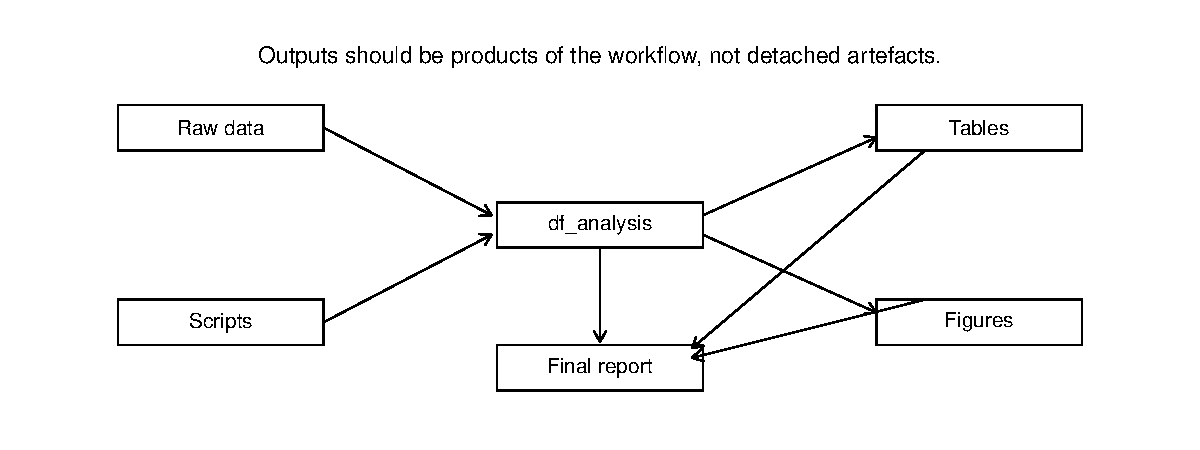
\includegraphics[width=0.9\linewidth,height=\textheight,keepaspectratio,alt={A simple diagram showing raw data and scripts feeding processed data, which then feeds tables, figures, and a final Quarto report.}]{chapters/25-final-integration-project_files/figure-pdf/fig-25-final-output-flow-1.pdf}

}

\caption{\label{fig-25-final-output-flow}How Final Project Outputs
Should Remain Connected to Their Sources.}

\end{figure}%

The message in Figure~\ref{fig-25-final-output-flow} is simple: the
final report should not be a manually assembled exhibition. It should be
a rebuildable product of the project.

\section{Step 1: Prepare the Project
Environment}\label{step-1-prepare-the-project-environment}

The final project begins before analysis. Leo first confirms that the
project has the packages, folders, and assumptions needed to rebuild the
work.

This step belongs near the beginning because environment problems are
silent project breakers. A workflow can be conceptually correct and
still fail because a folder does not exist, a package is missing, or the
project is being run from the wrong location.

The setup script should do limited work:

\begin{itemize}
\tightlist
\item
  load required packages
\item
  create expected folders
\item
  confirm expected input paths
\item
  avoid changing raw data
\item
  avoid producing final analysis claims
\end{itemize}

Leo already learned in
\hyperref[reliability-and-automation-making-workflows-repeatable]{Chapter
23} that automation is not just speed. It is ordered rebuilding. In
Chapter 25, the setup script becomes the first step in that order.

Listing~\ref{lst-25-setup-script} gives Leo a compact setup template. It
is non-evaluated because file creation belongs in the reader's project,
not inside the book render.

\begin{codelisting}

\caption{\label{lst-25-setup-script}A Setup Script Template for
Preparing the Final Integration Project.}

\centering{

\begin{Shaded}
\begin{Highlighting}[]
\CommentTok{\# scripts/00\_setup\_env.R}

\NormalTok{required\_packages }\OtherTok{\textless{}{-}} \FunctionTok{c}\NormalTok{(}
  \StringTok{"readr"}\NormalTok{,}
  \StringTok{"dplyr"}\NormalTok{,}
  \StringTok{"stringr"}\NormalTok{,}
  \StringTok{"lubridate"}\NormalTok{,}
  \StringTok{"ggplot2"}\NormalTok{,}
  \StringTok{"knitr"}
\NormalTok{)}

\NormalTok{missing\_packages }\OtherTok{\textless{}{-}}\NormalTok{ required\_packages[}
  \SpecialCharTok{!}\FunctionTok{vapply}\NormalTok{(required\_packages, requireNamespace, }\FunctionTok{logical}\NormalTok{(}\DecValTok{1}\NormalTok{), }\AttributeTok{quietly =} \ConstantTok{TRUE}\NormalTok{)}
\NormalTok{]}

\ControlFlowTok{if}\NormalTok{ (}\FunctionTok{length}\NormalTok{(missing\_packages) }\SpecialCharTok{\textgreater{}} \DecValTok{0}\NormalTok{) \{}
  \FunctionTok{stop}\NormalTok{(}
    \StringTok{"Install these packages before rebuilding the project: "}\NormalTok{,}
    \FunctionTok{paste}\NormalTok{(missing\_packages, }\AttributeTok{collapse =} \StringTok{", "}\NormalTok{)}
\NormalTok{  )}
\NormalTok{\}}

\CommentTok{\# Quarto itself is normally checked from the terminal with:}
\CommentTok{\# quarto {-}{-}version}

\NormalTok{required\_folders }\OtherTok{\textless{}{-}} \FunctionTok{c}\NormalTok{(}
  \StringTok{"data/raw"}\NormalTok{,}
  \StringTok{"data/processed"}\NormalTok{,}
  \StringTok{"scripts"}\NormalTok{,}
  \StringTok{"reports"}\NormalTok{,}
  \StringTok{"outputs/tables"}\NormalTok{,}
  \StringTok{"outputs/figures"}
\NormalTok{)}

\ControlFlowTok{for}\NormalTok{ (folder }\ControlFlowTok{in}\NormalTok{ required\_folders) \{}
  \ControlFlowTok{if}\NormalTok{ (}\SpecialCharTok{!}\FunctionTok{dir.exists}\NormalTok{(folder)) \{}
    \FunctionTok{dir.create}\NormalTok{(folder, }\AttributeTok{recursive =} \ConstantTok{TRUE}\NormalTok{)}
\NormalTok{  \}}
\NormalTok{\}}

\NormalTok{raw\_path }\OtherTok{\textless{}{-}} \StringTok{"data/raw/df\_r\_migration\_messy.csv"}

\ControlFlowTok{if}\NormalTok{ (}\SpecialCharTok{!}\FunctionTok{file.exists}\NormalTok{(raw\_path)) \{}
  \FunctionTok{stop}\NormalTok{(}
    \StringTok{"The raw dataset is missing. Expected file: "}\NormalTok{,}
\NormalTok{    raw\_path}
\NormalTok{  )}
\NormalTok{\}}
\end{Highlighting}
\end{Shaded}

}

\end{codelisting}%

The important habit in Listing~\ref{lst-25-setup-script} is not the list
of packages itself. It is the decision to make project assumptions
explicit before any analysis begins.

\section{Step 2: Import the Raw Learner
Data}\label{step-2-import-the-raw-learner-data}

The official raw data route is:

\texttt{data/raw/df\_r\_migration\_messy.csv}

The import script should make that route explicit. Leo should not import
from a downloads folder. He should not use a full machine-specific path
such as \texttt{C:/Users/Leo/Desktop/...}. The project must be able to
move.

A good import step does three things. It reads the file. It performs
immediate inspection. It stops early if the expected file is missing.

Listing~\ref{lst-25-import-script} shows the import step as a separate
script. It is not evaluated during book rendering because it depends on
the reader's project files.

\begin{codelisting}

\caption{\label{lst-25-import-script}An Import Script Template for
Reading and Inspecting the Raw Learner Data.}

\centering{

\begin{Shaded}
\begin{Highlighting}[]
\CommentTok{\# scripts/01\_import\_data.R}

\FunctionTok{source}\NormalTok{(}\StringTok{"scripts/00\_setup\_env.R"}\NormalTok{)}

\NormalTok{raw\_path }\OtherTok{\textless{}{-}} \StringTok{"data/raw/df\_r\_migration\_messy.csv"}

\ControlFlowTok{if}\NormalTok{ (}\SpecialCharTok{!}\FunctionTok{file.exists}\NormalTok{(raw\_path)) \{}
  \FunctionTok{stop}\NormalTok{(}\StringTok{"Cannot import data because the raw file is missing: "}\NormalTok{, raw\_path)}
\NormalTok{\}}

\NormalTok{raw\_migration }\OtherTok{\textless{}{-}}\NormalTok{ readr}\SpecialCharTok{::}\FunctionTok{read\_csv}\NormalTok{(}
\NormalTok{  raw\_path,}
  \AttributeTok{show\_col\_types =} \ConstantTok{FALSE}
\NormalTok{)}

\FunctionTok{message}\NormalTok{(}\StringTok{"Imported rows: "}\NormalTok{, }\FunctionTok{nrow}\NormalTok{(raw\_migration))}
\FunctionTok{message}\NormalTok{(}\StringTok{"Imported columns: "}\NormalTok{, }\FunctionTok{ncol}\NormalTok{(raw\_migration))}

\FunctionTok{print}\NormalTok{(}\FunctionTok{names}\NormalTok{(raw\_migration))}
\FunctionTok{print}\NormalTok{(dplyr}\SpecialCharTok{::}\FunctionTok{glimpse}\NormalTok{(raw\_migration))}
\end{Highlighting}
\end{Shaded}

}

\end{codelisting}%

The import script in Listing~\ref{lst-25-import-script} does not clean
the data. That boundary matters. Importing asks R to interpret a file as
data. Cleaning comes next.

\section{Step 3: Clean and Prepare the
Evidence}\label{step-3-clean-and-prepare-the-evidence}

Cleaning is the stabilisation layer. It protects everything downstream.

For this project, cleaning may include:

\begin{itemize}
\tightlist
\item
  standardising column names
\item
  trimming text fields
\item
  harmonising inconsistent categories
\item
  converting dates
\item
  converting numeric-looking text to numeric values
\item
  handling missing-like values such as blanks, \texttt{NA},
  \texttt{N/A}, \texttt{missing}, and \texttt{not\ available}
\item
  checking duplicate learner records or learner-week records
\item
  identifying suspicious values such as negative \texttt{study\_hours}
\item
  documenting decisions rather than hiding them
\end{itemize}

Cleaning must not become silent rewriting. Leo should be able to explain
what changed and why.
\hyperref[cleaning-and-preparing-data-making-evidence-trustworthy]{Chapter
13} made this distinction clear: cleaning makes evidence consistent
enough to analyse without hiding what was changed.

Listing~\ref{lst-25-clean-script} gives Leo a compact cleaning template.
It is deliberately not exhaustive. The point is to show how cleaning
decisions are made visible and repeatable.

\begin{codelisting}

\caption{\label{lst-25-clean-script}A Cleaning Script Template for
Preparing the Learner Dataset.}

\centering{

\begin{Shaded}
\begin{Highlighting}[]
\CommentTok{\# scripts/02\_clean\_data.R}

\FunctionTok{source}\NormalTok{(}\StringTok{"scripts/01\_import\_data.R"}\NormalTok{)}

\NormalTok{missing\_like\_values }\OtherTok{\textless{}{-}} \FunctionTok{c}\NormalTok{(}
  \StringTok{""}\NormalTok{,}
  \StringTok{"NA"}\NormalTok{,}
  \StringTok{"N/A"}\NormalTok{,}
  \StringTok{"missing"}\NormalTok{,}
  \StringTok{"not available"}\NormalTok{,}
  \StringTok{"Not available"}
\NormalTok{)}

\NormalTok{df\_clean }\OtherTok{\textless{}{-}}\NormalTok{ raw\_migration }\SpecialCharTok{|\textgreater{}}
\NormalTok{  dplyr}\SpecialCharTok{::}\FunctionTok{mutate}\NormalTok{(}
\NormalTok{    dplyr}\SpecialCharTok{::}\FunctionTok{across}\NormalTok{(}
      \FunctionTok{where}\NormalTok{(is.character),}
      \SpecialCharTok{\textasciitilde{}}\NormalTok{ stringr}\SpecialCharTok{::}\FunctionTok{str\_squish}\NormalTok{(.x)}
\NormalTok{    ),}
\NormalTok{    dplyr}\SpecialCharTok{::}\FunctionTok{across}\NormalTok{(}
      \FunctionTok{where}\NormalTok{(is.character),}
      \SpecialCharTok{\textasciitilde{}}\NormalTok{ dplyr}\SpecialCharTok{::}\FunctionTok{na\_if}\NormalTok{(.x, }\StringTok{""}\NormalTok{)}
\NormalTok{    )}
\NormalTok{  ) }\SpecialCharTok{|\textgreater{}}
\NormalTok{  dplyr}\SpecialCharTok{::}\FunctionTok{mutate}\NormalTok{(}
\NormalTok{    dplyr}\SpecialCharTok{::}\FunctionTok{across}\NormalTok{(}
      \FunctionTok{where}\NormalTok{(is.character),}
      \SpecialCharTok{\textasciitilde{}} \FunctionTok{ifelse}\NormalTok{(.x }\SpecialCharTok{\%in\%}\NormalTok{ missing\_like\_values, }\ConstantTok{NA}\NormalTok{, .x)}
\NormalTok{    ),}
    \AttributeTok{country =}\NormalTok{ stringr}\SpecialCharTok{::}\FunctionTok{str\_to\_title}\NormalTok{(country),}
    \AttributeTok{background =}\NormalTok{ stringr}\SpecialCharTok{::}\FunctionTok{str\_to\_title}\NormalTok{(background),}
    \AttributeTok{industry =}\NormalTok{ stringr}\SpecialCharTok{::}\FunctionTok{str\_to\_title}\NormalTok{(industry),}
    \AttributeTok{job\_role =}\NormalTok{ stringr}\SpecialCharTok{::}\FunctionTok{str\_to\_title}\NormalTok{(job\_role),}
    \AttributeTok{completion\_status =}\NormalTok{ stringr}\SpecialCharTok{::}\FunctionTok{str\_to\_title}\NormalTok{(completion\_status),}
    \AttributeTok{study\_hours =} \FunctionTok{suppressWarnings}\NormalTok{(}\FunctionTok{as.numeric}\NormalTok{(study\_hours)),}
    \AttributeTok{lessons\_completed =} \FunctionTok{suppressWarnings}\NormalTok{(}\FunctionTok{as.numeric}\NormalTok{(lessons\_completed)),}
    \AttributeTok{confidence\_score =} \FunctionTok{suppressWarnings}\NormalTok{(}\FunctionTok{as.numeric}\NormalTok{(confidence\_score)),}
    \AttributeTok{project\_score =} \FunctionTok{suppressWarnings}\NormalTok{(}\FunctionTok{as.numeric}\NormalTok{(project\_score))}
\NormalTok{  )}

\NormalTok{suspicious\_study\_hours }\OtherTok{\textless{}{-}}\NormalTok{ df\_clean }\SpecialCharTok{|\textgreater{}}
\NormalTok{  dplyr}\SpecialCharTok{::}\FunctionTok{filter}\NormalTok{(}\SpecialCharTok{!}\FunctionTok{is.na}\NormalTok{(study\_hours), study\_hours }\SpecialCharTok{\textless{}} \DecValTok{0}\NormalTok{)}

\ControlFlowTok{if}\NormalTok{ (}\FunctionTok{nrow}\NormalTok{(suspicious\_study\_hours) }\SpecialCharTok{\textgreater{}} \DecValTok{0}\NormalTok{) \{}
  \FunctionTok{warning}\NormalTok{(}
    \StringTok{"Some records have negative study\_hours. Inspect before interpretation."}
\NormalTok{  )}
\NormalTok{\}}
\end{Highlighting}
\end{Shaded}

}

\end{codelisting}%

The template in Listing~\ref{lst-25-clean-script} is a disciplined
starting point, not a magical cleaning machine. Leo should revise it
when the real inspection reveals additional problems.

\section{Step 4: Create the Analysis-Ready
Dataset}\label{step-4-create-the-analysis-ready-dataset}

The analysis-ready object is the bridge between preparation and
interpretation.

In this book, the central object is:

\texttt{df\_analysis}

The saved versions are:

\texttt{data/processed/df\_analysis.rds}

and:

\texttt{data/processed/df\_analysis.csv}

The \texttt{.rds} file preserves R object structure. The \texttt{.csv}
file is useful for sharing with people or systems outside R. Leo does
not need to choose one forever. He needs to know why each exists.

Listing~\ref{lst-25-analysis-data-script} shows how the cleaned evidence
can become the final analysis-ready object. It is non-evaluated because
it writes files in the reader's project.

\begin{codelisting}

\caption{\label{lst-25-analysis-data-script}A Script Template for
Creating and Saving the Analysis-Ready Dataset.}

\centering{

\begin{Shaded}
\begin{Highlighting}[]
\CommentTok{\# scripts/03\_create\_analysis\_data.R}

\FunctionTok{source}\NormalTok{(}\StringTok{"scripts/02\_clean\_data.R"}\NormalTok{)}

\NormalTok{df\_analysis }\OtherTok{\textless{}{-}}\NormalTok{ df\_clean }\SpecialCharTok{|\textgreater{}}
\NormalTok{  dplyr}\SpecialCharTok{::}\FunctionTok{mutate}\NormalTok{(}
    \AttributeTok{project\_ready =}\NormalTok{ dplyr}\SpecialCharTok{::}\FunctionTok{case\_when}\NormalTok{(}
      \SpecialCharTok{!}\FunctionTok{is.na}\NormalTok{(project\_score) }\SpecialCharTok{\&}
        \SpecialCharTok{!}\FunctionTok{is.na}\NormalTok{(confidence\_score) }\SpecialCharTok{\&}
\NormalTok{        project\_score }\SpecialCharTok{\textgreater{}=} \DecValTok{70} \SpecialCharTok{\&}
\NormalTok{        confidence\_score }\SpecialCharTok{\textgreater{}=} \DecValTok{70} \SpecialCharTok{\textasciitilde{}} \StringTok{"Project{-}ready indicator met"}\NormalTok{,}
      \ConstantTok{TRUE} \SpecialCharTok{\textasciitilde{}} \StringTok{"Project{-}ready indicator not met"}
\NormalTok{    ),}
    \AttributeTok{study\_band =} \FunctionTok{cut}\NormalTok{(}
\NormalTok{      study\_hours,}
      \AttributeTok{breaks =} \FunctionTok{c}\NormalTok{(}\SpecialCharTok{{-}}\ConstantTok{Inf}\NormalTok{, }\DecValTok{3}\NormalTok{, }\DecValTok{6}\NormalTok{, }\DecValTok{9}\NormalTok{, }\ConstantTok{Inf}\NormalTok{),}
      \AttributeTok{labels =} \FunctionTok{c}\NormalTok{(}
        \StringTok{"Up to 3 hours"}\NormalTok{,}
        \StringTok{"More than 3 to 6"}\NormalTok{,}
        \StringTok{"More than 6 to 9"}\NormalTok{,}
        \StringTok{"More than 9"}
\NormalTok{      )}
\NormalTok{    )}
\NormalTok{  )}

\NormalTok{required\_analysis\_columns }\OtherTok{\textless{}{-}} \FunctionTok{c}\NormalTok{(}
  \StringTok{"learner\_id"}\NormalTok{,}
  \StringTok{"country"}\NormalTok{,}
  \StringTok{"background"}\NormalTok{,}
  \StringTok{"study\_hours"}\NormalTok{,}
  \StringTok{"lessons\_completed"}\NormalTok{,}
  \StringTok{"confidence\_score"}\NormalTok{,}
  \StringTok{"project\_score"}\NormalTok{,}
  \StringTok{"completion\_status"}\NormalTok{,}
  \StringTok{"project\_ready"}
\NormalTok{)}

\NormalTok{missing\_analysis\_columns }\OtherTok{\textless{}{-}} \FunctionTok{setdiff}\NormalTok{(}
\NormalTok{  required\_analysis\_columns,}
  \FunctionTok{names}\NormalTok{(df\_analysis)}
\NormalTok{)}

\ControlFlowTok{if}\NormalTok{ (}\FunctionTok{length}\NormalTok{(missing\_analysis\_columns) }\SpecialCharTok{\textgreater{}} \DecValTok{0}\NormalTok{) \{}
  \FunctionTok{stop}\NormalTok{(}
    \StringTok{"The analysis{-}ready dataset is missing required columns: "}\NormalTok{,}
    \FunctionTok{paste}\NormalTok{(missing\_analysis\_columns, }\AttributeTok{collapse =} \StringTok{", "}\NormalTok{)}
\NormalTok{  )}
\NormalTok{\}}

\FunctionTok{saveRDS}\NormalTok{(df\_analysis, }\StringTok{"data/processed/df\_analysis.rds"}\NormalTok{)}
\NormalTok{readr}\SpecialCharTok{::}\FunctionTok{write\_csv}\NormalTok{(df\_analysis, }\StringTok{"data/processed/df\_analysis.csv"}\NormalTok{)}
\end{Highlighting}
\end{Shaded}

}

\end{codelisting}%

The file-writing lines in Listing~\ref{lst-25-analysis-data-script}
belong inside the reader's project workflow, not inside the rendered
book chapter. That is why the listing is non-evaluated.

Listing~\ref{lst-25-script-sequence} shows the script order for
rebuilding the final project from the terminal. It is also non-evaluated
because it represents the project execution pattern, not a chunk that
should run during book rendering.

\begin{codelisting}

\caption{\label{lst-25-script-sequence}A Script Sequence for Rebuilding
the Final Integration Project.}

\centering{

\begin{Shaded}
\begin{Highlighting}[]
\ExtensionTok{Rscript}\NormalTok{ scripts/00\_setup\_env.R}
\ExtensionTok{Rscript}\NormalTok{ scripts/01\_import\_data.R}
\ExtensionTok{Rscript}\NormalTok{ scripts/02\_clean\_data.R}
\ExtensionTok{Rscript}\NormalTok{ scripts/03\_create\_analysis\_data.R}
\ExtensionTok{Rscript}\NormalTok{ scripts/04\_validate\_outputs.R}
\ExtensionTok{quarto}\NormalTok{ render reports/final{-}integration{-}report.qmd}
\end{Highlighting}
\end{Shaded}

}

\end{codelisting}%

The order in Listing~\ref{lst-25-script-sequence} is more important than
the specific terminal style. Leo's machine may use RStudio, the
terminal, or another editor. The professional habit remains the same:
rebuild the project in a known order.

\section{Step 5: Validate Assumptions and
Outputs}\label{step-5-validate-assumptions-and-outputs}

Validation is where Leo refuses to trust a beautiful output too quickly.

A final integration project should check that the object being analysed
has the expected columns, plausible values, and enough rows to support
the report. These checks do not make the analysis perfect. They reduce
the risk of silent error.

Listing~\ref{lst-25-validation-script} shows how Leo can place
validation checks in a dedicated script. It is non-evaluated because it
depends on the project object created outside the book render.

\begin{codelisting}

\caption{\label{lst-25-validation-script}A Validation Script Template
for Checking the Final Analysis Object.}

\centering{

\begin{Shaded}
\begin{Highlighting}[]
\CommentTok{\# scripts/04\_validate\_outputs.R}

\NormalTok{analysis\_path }\OtherTok{\textless{}{-}} \StringTok{"data/processed/df\_analysis.rds"}

\ControlFlowTok{if}\NormalTok{ (}\SpecialCharTok{!}\FunctionTok{file.exists}\NormalTok{(analysis\_path)) \{}
  \FunctionTok{stop}\NormalTok{(}\StringTok{"The analysis{-}ready file is missing: "}\NormalTok{, analysis\_path)}
\NormalTok{\}}

\NormalTok{df\_analysis }\OtherTok{\textless{}{-}} \FunctionTok{readRDS}\NormalTok{(analysis\_path)}

\NormalTok{required\_columns }\OtherTok{\textless{}{-}} \FunctionTok{c}\NormalTok{(}
  \StringTok{"learner\_id"}\NormalTok{,}
  \StringTok{"country"}\NormalTok{,}
  \StringTok{"study\_hours"}\NormalTok{,}
  \StringTok{"lessons\_completed"}\NormalTok{,}
  \StringTok{"confidence\_score"}\NormalTok{,}
  \StringTok{"project\_score"}\NormalTok{,}
  \StringTok{"completion\_status"}\NormalTok{,}
  \StringTok{"project\_ready"}
\NormalTok{)}

\NormalTok{missing\_columns }\OtherTok{\textless{}{-}} \FunctionTok{setdiff}\NormalTok{(required\_columns, }\FunctionTok{names}\NormalTok{(df\_analysis))}

\ControlFlowTok{if}\NormalTok{ (}\FunctionTok{length}\NormalTok{(missing\_columns) }\SpecialCharTok{\textgreater{}} \DecValTok{0}\NormalTok{) \{}
  \FunctionTok{stop}\NormalTok{(}
    \StringTok{"The analysis object is missing required columns: "}\NormalTok{,}
    \FunctionTok{paste}\NormalTok{(missing\_columns, }\AttributeTok{collapse =} \StringTok{", "}\NormalTok{)}
\NormalTok{  )}
\NormalTok{\}}

\ControlFlowTok{if}\NormalTok{ (}\FunctionTok{nrow}\NormalTok{(df\_analysis) }\SpecialCharTok{==} \DecValTok{0}\NormalTok{) \{}
  \FunctionTok{stop}\NormalTok{(}\StringTok{"The analysis object has no rows."}\NormalTok{)}
\NormalTok{\}}

\ControlFlowTok{if}\NormalTok{ (}\FunctionTok{any}\NormalTok{(}\FunctionTok{is.na}\NormalTok{(df\_analysis}\SpecialCharTok{$}\NormalTok{learner\_id))) \{}
  \FunctionTok{stop}\NormalTok{(}\StringTok{"Some learner\_id values are missing."}\NormalTok{)}
\NormalTok{\}}

\ControlFlowTok{if}\NormalTok{ (}\FunctionTok{any}\NormalTok{(df\_analysis}\SpecialCharTok{$}\NormalTok{study\_hours }\SpecialCharTok{\textless{}} \DecValTok{0}\NormalTok{, }\AttributeTok{na.rm =} \ConstantTok{TRUE}\NormalTok{)) \{}
  \FunctionTok{stop}\NormalTok{(}\StringTok{"Some study\_hours values are negative."}\NormalTok{)}
\NormalTok{\}}

\ControlFlowTok{if}\NormalTok{ (}\FunctionTok{any}\NormalTok{(}
\NormalTok{  df\_analysis}\SpecialCharTok{$}\NormalTok{project\_score }\SpecialCharTok{\textless{}} \DecValTok{0} \SpecialCharTok{|}\NormalTok{ df\_analysis}\SpecialCharTok{$}\NormalTok{project\_score }\SpecialCharTok{\textgreater{}} \DecValTok{100}\NormalTok{,}
  \AttributeTok{na.rm =} \ConstantTok{TRUE}
\NormalTok{)) \{}
  \FunctionTok{stop}\NormalTok{(}\StringTok{"Some project\_score values fall outside 0 to 100."}\NormalTok{)}
\NormalTok{\}}

\ControlFlowTok{if}\NormalTok{ (}\FunctionTok{any}\NormalTok{(}
\NormalTok{  df\_analysis}\SpecialCharTok{$}\NormalTok{confidence\_score }\SpecialCharTok{\textless{}} \DecValTok{0} \SpecialCharTok{|}\NormalTok{ df\_analysis}\SpecialCharTok{$}\NormalTok{confidence\_score }\SpecialCharTok{\textgreater{}} \DecValTok{100}\NormalTok{,}
  \AttributeTok{na.rm =} \ConstantTok{TRUE}
\NormalTok{)) \{}
  \FunctionTok{stop}\NormalTok{(}\StringTok{"Some confidence\_score values fall outside 0 to 100."}\NormalTok{)}
\NormalTok{\}}

\FunctionTok{message}\NormalTok{(}\StringTok{"Validation checks completed."}\NormalTok{)}
\end{Highlighting}
\end{Shaded}

}

\end{codelisting}%

Table~\ref{tbl-25-validation-checks} demonstrates a small validation
summary for the current render. When the official processed dataset
exists, the checks reflect that object. When the book is rendered
without the project data available, the setup chunk uses a small
render-safe example so the chapter still compiles. The table is a
workflow demonstration, not a substantive research finding.

{

\begin{longtable}[]{@{}
  >{\raggedright\arraybackslash}p{(\linewidth - 2\tabcolsep) * \real{0.6737}}
  >{\raggedright\arraybackslash}p{(\linewidth - 2\tabcolsep) * \real{0.3263}}@{}}

\caption{\label{tbl-25-validation-checks}A Render-Safe Validation
Summary for the Chapter 25 Final Project.}

\tabularnewline

\toprule\noalign{}
\begin{minipage}[b]{\linewidth}\raggedright
Check
\end{minipage} & \begin{minipage}[b]{\linewidth}\raggedright
Result
\end{minipage} \\
\midrule\noalign{}
\endhead
\bottomrule\noalign{}
\endlastfoot
Data source used for this render & data/processed/df\_analysis.rds \\
Dataset contains at least one row & Pass \\
Required project columns are present & Pass \\
Learner ID column has no missing values & Pass \\
Study hours has no negative values among non-missing entries & Pass \\
Project score is between 0 and 100 among non-missing entries & Pass \\
Confidence score is between 0 and 100 among non-missing entries &
Pass \\
Completion status column exists for interpretation & Pass \\

\end{longtable}

}

The point of Table~\ref{tbl-25-validation-checks} is not to make Leo
paranoid. It is to make him disciplined. If a check fails, he should
pause, inspect the relevant stage, and correct the workflow rather than
editing the final report by hand.

\begin{tcolorbox}[enhanced jigsaw, arc=.35mm, bottomrule=.15mm, bottomtitle=1mm, breakable, colback=white, colbacktitle=quarto-callout-tip-color!10!white, colframe=quarto-callout-tip-color-frame, coltitle=black, left=2mm, leftrule=.75mm, opacityback=0, opacitybacktitle=0.6, rightrule=.15mm, title=\textcolor{quarto-callout-tip-color}{\faLightbulb}\hspace{0.5em}{Validate before interpreting}, titlerule=0mm, toprule=.15mm, toptitle=1mm]

A final table or figure is only as trustworthy as the route that
produced it. Before Leo discusses a pattern, he should confirm that the
object, variables, and assumptions behind that pattern are sound.

\end{tcolorbox}

\section{Step 6: Summarise the
Evidence}\label{step-6-summarise-the-evidence}

A final project needs summaries that serve the analytical question. It
does not need every possible table.

For the learner project, useful summaries might include:

\begin{itemize}
\tightlist
\item
  learner counts by completion status
\item
  average project scores by completion status
\item
  average confidence scores by study-hour bands
\item
  differences in project scores across experience levels or backgrounds
\item
  the relationship among lessons completed, study hours, confidence, and
  project performance
\end{itemize}

Leo should not treat these as isolated outputs. Each table should answer
a defined part of the final question.

Table~\ref{tbl-25-evidence-summary} gives a small render-safe example of
the kind of table the final report may include. The table groups
learners by study-hour band and reports project readiness indicators.
Its purpose is instructional: it shows how a final table can be tied to
the analytical question without pretending to prove causation.

{

\begin{longtable}[]{@{}
  >{\raggedright\arraybackslash}p{(\linewidth - 8\tabcolsep) * \real{0.1619}}
  >{\raggedright\arraybackslash}p{(\linewidth - 8\tabcolsep) * \real{0.0857}}
  >{\raggedright\arraybackslash}p{(\linewidth - 8\tabcolsep) * \real{0.2381}}
  >{\raggedright\arraybackslash}p{(\linewidth - 8\tabcolsep) * \real{0.2095}}
  >{\raggedright\arraybackslash}p{(\linewidth - 8\tabcolsep) * \real{0.3048}}@{}}

\caption{\label{tbl-25-evidence-summary}A Render-Safe Example Summary
Linking Study Effort, Confidence, and Project Readiness.}

\tabularnewline

\toprule\noalign{}
\begin{minipage}[b]{\linewidth}\raggedright
Study-hour band
\end{minipage} & \begin{minipage}[b]{\linewidth}\raggedright
Learners
\end{minipage} & \begin{minipage}[b]{\linewidth}\raggedright
Average confidence score
\end{minipage} & \begin{minipage}[b]{\linewidth}\raggedright
Average project score
\end{minipage} & \begin{minipage}[b]{\linewidth}\raggedright
Project-ready indicator met (\%)
\end{minipage} \\
\midrule\noalign{}
\endhead
\bottomrule\noalign{}
\endlastfoot
Up to 3 hours & 10 & 74.8 & 76.2 & 30.0 \\
More than 3 to 6 & 28 & 63.9 & 72.7 & 17.9 \\
More than 6 to 9 & 98 & 70.6 & 78.3 & 30.6 \\
More than 9 & 448 & 71.4 & 82.0 & 36.6 \\

\end{longtable}

}

A careful final report would discuss Table~\ref{tbl-25-evidence-summary}
with restraint. If higher study bands appear stronger, Leo may describe
an association in the dataset. He should not claim that study hours
alone caused project readiness unless the research design supports that
claim.

A good final report might move through three questions:

\begin{enumerate}
\def\labelenumi{\arabic{enumi}.}
\tightlist
\item
  Who is represented in the learner dataset?
\item
  What patterns are visible across learning effort, confidence,
  completion, tool use, and project performance?
\item
  What practical interpretation can be made without overstating the
  evidence?
\end{enumerate}

This is where judgement matters. The final project is not an excuse to
produce twenty tables. It is a chance to produce a small number of
credible outputs.

\section{Step 7: Visualise the
Findings}\label{step-7-visualise-the-findings}

Figures in the final project should clarify patterns that tables alone
make slow to see.

A figure might show project score by study hours, confidence score by
completion status, or completion patterns across countries or
backgrounds. Leo should choose a figure because it helps the reader
understand the evidence, not because the report feels empty without one.

The final chapter should also remind Leo of a principle from the
visualisation chapters: a figure is not a decoration. It is an argument
in visual form.

Listing~\ref{lst-25-visualisation-template} gives Leo a simple
report-ready plotting pattern. It is non-evaluated because the final
report, not the book chapter, should create project-specific figures
from the reader's local \texttt{df\_analysis}.

\begin{codelisting}

\caption{\label{lst-25-visualisation-template}A Visualisation Template
for Connecting Project Scores and Study Effort.}

\centering{

\begin{Shaded}
\begin{Highlighting}[]
\CommentTok{\# Inside reports/final{-}integration{-}report.qmd}

\NormalTok{df\_analysis }\OtherTok{\textless{}{-}} \FunctionTok{readRDS}\NormalTok{(}\StringTok{"data/processed/df\_analysis.rds"}\NormalTok{)}

\NormalTok{ggplot2}\SpecialCharTok{::}\FunctionTok{ggplot}\NormalTok{(}
\NormalTok{  df\_analysis,}
\NormalTok{  ggplot2}\SpecialCharTok{::}\FunctionTok{aes}\NormalTok{(}
    \AttributeTok{x =}\NormalTok{ study\_hours,}
    \AttributeTok{y =}\NormalTok{ project\_score}
\NormalTok{  )}
\NormalTok{) }\SpecialCharTok{+}
\NormalTok{  ggplot2}\SpecialCharTok{::}\FunctionTok{geom\_point}\NormalTok{(}\AttributeTok{na.rm =} \ConstantTok{TRUE}\NormalTok{) }\SpecialCharTok{+}
\NormalTok{  ggplot2}\SpecialCharTok{::}\FunctionTok{geom\_smooth}\NormalTok{(}
    \AttributeTok{method =} \StringTok{"lm"}\NormalTok{,}
    \AttributeTok{se =} \ConstantTok{FALSE}\NormalTok{,}
    \AttributeTok{na.rm =} \ConstantTok{TRUE}
\NormalTok{  ) }\SpecialCharTok{+}
\NormalTok{  ggplot2}\SpecialCharTok{::}\FunctionTok{labs}\NormalTok{(}
    \AttributeTok{title =} \StringTok{"Project Score and Study Hours"}\NormalTok{,}
    \AttributeTok{x =} \StringTok{"Weekly study hours"}\NormalTok{,}
    \AttributeTok{y =} \StringTok{"Project score"}
\NormalTok{  )}
\end{Highlighting}
\end{Shaded}

}

\end{codelisting}%

The plotting template in Listing~\ref{lst-25-visualisation-template} is
intentionally modest. Leo has already learned how to improve clarity and
storytelling in the visualisation chapters. The final point here is not
a new plotting trick. It is that the figure must be produced from the
same analysis-ready object used by the rest of the report.

\section{Step 8: Render the Final Quarto
Report}\label{step-8-render-the-final-quarto-report}

The final report is the public face of the analytical system. It should
contain:

\begin{itemize}
\tightlist
\item
  a short project question
\item
  a data source note
\item
  cleaning and preparation summary
\item
  validation summary
\item
  key tables
\item
  key figures
\item
  interpretation
\item
  limitations
\item
  reproducibility note
\end{itemize}

The report should not require Leo to paste screenshots or manually
insert values. It should rebuild from the workflow.

Listing~\ref{lst-25-report-scaffold} gives Leo a non-evaluated report
scaffold. It is not intended to replace the full chapter. It shows the
kind of structure a final report can use.

\begin{codelisting}

\caption{\label{lst-25-report-scaffold}A Quarto Report Scaffold for the
Final Integration Project.}

\centering{

\begin{Shaded}
\begin{Highlighting}[]
\CommentTok{\# Save this as reports/final{-}integration{-}report.qmd}

\CommentTok{\# {-}{-}{-}}
\CommentTok{\# title: "Final Integration Report"}
\CommentTok{\# format: html}
\CommentTok{\# {-}{-}{-}}

\CommentTok{\# \#\# Project Question}
\CommentTok{\#}
\CommentTok{\# What factors appear to support a learner\textquotesingle{}s movement from R beginner}
\CommentTok{\# to confident, project{-}ready analyst?}

\CommentTok{\# \#\# Data Source}
\CommentTok{\#}
\CommentTok{\# This report uses data/processed/df\_analysis.rds, created from}
\CommentTok{\# data/raw/df\_r\_migration\_messy.csv.}

\NormalTok{df\_analysis }\OtherTok{\textless{}{-}} \FunctionTok{readRDS}\NormalTok{(}\StringTok{"data/processed/df\_analysis.rds"}\NormalTok{)}

\CommentTok{\# \#\# Validation Summary}
\CommentTok{\#}
\CommentTok{\# Add required{-}column, row{-}count, missing{-}value, and range checks here.}

\CommentTok{\# \#\# Key Summaries}
\CommentTok{\#}
\CommentTok{\# Create final summary tables here.}

\CommentTok{\# \#\# Key Figures}
\CommentTok{\#}
\CommentTok{\# Create final figures here.}

\CommentTok{\# \#\# Interpretation}
\CommentTok{\#}
\CommentTok{\# Explain what the evidence suggests, what it does not prove, and what}
\CommentTok{\# a careful reader should take from the analysis.}

\CommentTok{\# \#\# Limitations}
\CommentTok{\#}
\CommentTok{\# State the limits of the dataset, missing values, cleaning decisions,}
\CommentTok{\# and the difference between association and causation.}

\CommentTok{\# \#\# Reproducibility Note}
\CommentTok{\#}
\CommentTok{\# State how the report can be rebuilt and which data object it uses.}
\end{Highlighting}
\end{Shaded}

}

\end{codelisting}%

After writing the report, Leo should render it through a clear command.
Listing~\ref{lst-25-render-command} shows the terminal pattern. It is
non-evaluated because terminal commands should be run in the terminal,
not inside the R Console.

\begin{codelisting}

\caption{\label{lst-25-render-command}A Terminal Command for Rendering
the Final Integration Report.}

\centering{

\begin{Shaded}
\begin{Highlighting}[]
\ExtensionTok{quarto}\NormalTok{ render reports/final{-}integration{-}report.qmd}
\end{Highlighting}
\end{Shaded}

}

\end{codelisting}%

If Leo renders the report and it fails, that failure is useful. It tells
him where the system is broken. He should not patch the HTML by hand. He
should fix the source.

\section{Step 9: Preserve the Work with Version
Control}\label{step-9-preserve-the-work-with-version-control}

A final project is not complete until its changes are traceable.

Version control does not make the analysis correct by itself. It makes
the project history visible. It allows Leo to see what changed, recover
from mistakes, and communicate progress.

Listing~\ref{lst-25-git-preservation} shows a minimal Git preservation
sequence for the final project.

\begin{codelisting}

\caption{\label{lst-25-git-preservation}A Minimal Git Sequence for
Preserving the Final Integration Project.}

\centering{

\begin{Shaded}
\begin{Highlighting}[]
\FunctionTok{git}\NormalTok{ status}
\FunctionTok{git}\NormalTok{ diff}
\FunctionTok{git}\NormalTok{ add scripts/}
\FunctionTok{git}\NormalTok{ add reports/final{-}integration{-}report.qmd}
\FunctionTok{git}\NormalTok{ add outputs/}
\FunctionTok{git}\NormalTok{ add data/processed/df\_analysis.rds}
\FunctionTok{git}\NormalTok{ add data/processed/df\_analysis.csv}
\FunctionTok{git}\NormalTok{ add README.md}
\FunctionTok{git}\NormalTok{ commit }\AttributeTok{{-}m} \StringTok{"Complete final integration project workflow"}
\FunctionTok{git}\NormalTok{ log }\AttributeTok{{-}{-}oneline}
\end{Highlighting}
\end{Shaded}

}

\end{codelisting}%

The important habit in Listing~\ref{lst-25-git-preservation} is not the
exact commit message. It is the discipline of inspecting before
recording. Leo should know what he is committing before he commits it.

There is one additional judgement. In a teaching project, the learner
dataset and processed outputs may be small enough to track. In a
workplace project, large, private, or sensitive data may need different
handling. The principle from
\hyperref[collaboration-and-version-control-making-work-traceable]{Chapter
21} still applies: version control should make work traceable without
carelessly exposing material that should not be shared.

\section{Step 10: Review Performance and
Scale}\label{step-10-review-performance-and-scale}

Chapter 25 should not repeat
\hyperref[performance-and-scale-making-r-work-efficiently]{Chapter 24},
but the final project must still respect it.

Before Leo calls the project complete, he should ask:

\begin{itemize}
\tightlist
\item
  Does the report rebuild in a reasonable time?
\item
  Is the workflow rereading large files unnecessarily?
\item
  Are expensive steps repeated when a stable processed object would be
  better?
\item
  Are intermediate objects named clearly?
\item
  Are optional high-performance tools being used only where they are
  justified?
\item
  Has speed been improved without damaging readability?
\end{itemize}

The final question is not, ``Did Leo make R as fast as possible?'' The
better question is, ``Can the project rebuild efficiently enough for
real use, while remaining clear enough to trust?''

This is where Chapter 24's lesson becomes part of the final system.
Correctness comes first. Bottlenecks should be identified before they
are fixed. Parallel computing, \texttt{foreach}, \texttt{apply}
patterns, vectorisation, databases, or columnar storage are not prizes
to display. They are responses to real constraints.

\section{The Final Project Checklist}\label{the-final-project-checklist}

A final checklist helps Leo resist the temptation to stop too early. The
report may render. The figure may look good. The table may appear
plausible. But the system is only ready when its major links are clear.

Table~\ref{tbl-25-final-checklist} gives Leo a final review tool before
calling the project complete.

{

\begin{longtable}[]{@{}
  >{\raggedright\arraybackslash}p{(\linewidth - 4\tabcolsep) * \real{0.1630}}
  >{\raggedright\arraybackslash}p{(\linewidth - 4\tabcolsep) * \real{0.6519}}
  >{\raggedright\arraybackslash}p{(\linewidth - 4\tabcolsep) * \real{0.1852}}@{}}

\caption{\label{tbl-25-final-checklist}Final Completion Checklist for
the Chapter 25 Integration Project.}

\tabularnewline

\toprule\noalign{}
\begin{minipage}[b]{\linewidth}\raggedright
Area
\end{minipage} & \begin{minipage}[b]{\linewidth}\raggedright
Completion question
\end{minipage} & \begin{minipage}[b]{\linewidth}\raggedright
Status before submission
\end{minipage} \\
\midrule\noalign{}
\endhead
\bottomrule\noalign{}
\endlastfoot
Project question & Is the final analytical question clear, bounded, and
answerable with the dataset? & Confirm \\
Raw data & Is the raw dataset stored in \texttt{data/raw/} without
manual alteration? & Confirm \\
Import route & Can the data be imported using a project-relative path? &
Confirm \\
Inspection & Has the imported object been inspected before cleaning or
interpretation? & Confirm \\
Cleaning decisions & Are cleaning choices visible, documented, and
separated from raw data? & Confirm \\
Analysis-ready object & Can \texttt{df\_analysis} be rebuilt and saved
to \texttt{data/processed/}? & Confirm \\
Validation & Do checks confirm required columns, plausible ranges, row
counts, and expected outputs? & Confirm \\
Tables & Does each table answer part of the final question? & Confirm \\
Figures & Does each figure clarify a pattern rather than decorate the
report? & Confirm \\
Report & Can the Quarto report render from source without manual
patching? & Confirm \\
Environment & Are packages and versions managed consistently enough for
the project? & Confirm \\
Version control & Are major changes inspected and committed with
meaningful messages? & Confirm \\
Performance & Does the project rebuild in a reasonable time without
unnecessary repeated work? & Confirm \\
Reader guidance & Would another careful reader know how to rerun and
inspect the project? & Confirm \\

\end{longtable}

}

This is the final professional habit: do not ask only whether the output
exists. Ask whether the route to the output is defensible.

\section{Common Integration Failures}\label{common-integration-failures}

By the final chapter, Leo has enough skill to make serious progress. He
also has enough skill to make more subtle mistakes.

The common failures are no longer only syntax errors. They are workflow
errors.

Table~\ref{tbl-25-integration-failures} lists the failure patterns Leo
should now be able to diagnose.

{

\begin{longtable}[]{@{}
  >{\raggedright\arraybackslash}p{(\linewidth - 4\tabcolsep) * \real{0.2536}}
  >{\raggedright\arraybackslash}p{(\linewidth - 4\tabcolsep) * \real{0.3780}}
  >{\raggedright\arraybackslash}p{(\linewidth - 4\tabcolsep) * \real{0.3684}}@{}}

\caption{\label{tbl-25-integration-failures}Common Integration Failures
and the Professional Habit That Prevents Each One.}

\tabularnewline

\toprule\noalign{}
\begin{minipage}[b]{\linewidth}\raggedright
Failure
\end{minipage} & \begin{minipage}[b]{\linewidth}\raggedright
Why it weakens the project
\end{minipage} & \begin{minipage}[b]{\linewidth}\raggedright
Better habit
\end{minipage} \\
\midrule\noalign{}
\endhead
\bottomrule\noalign{}
\endlastfoot
Changing raw data directly & The audit trail disappears and cleaning
decisions become difficult to explain. & Keep raw data untouched and
save processed objects separately. \\
Depending on hidden workspace objects & The report may work on one
machine but fail when the project is restarted. & Load or create every
required object inside the report or workflow. \\
Using absolute paths & The project becomes tied to one person's
computer. & Use project-relative paths. \\
Forgetting which script created which output & Outputs become detached
from the workflow that produced them. & Name scripts clearly and
document the execution order. \\
Saving tables or figures manually without code & The final report can
stop matching the current data and code. & Generate outputs from code or
make manual export decisions explicit. \\
Ignoring warnings because the report still rendered & A visible output
can hide a damaged assumption. & Read warnings and decide whether they
require action. \\
Letting old figures remain after the data changed & The reader may see
stale evidence without knowing it. & Regenerate outputs whenever data or
code changes. \\
Committing large or sensitive files carelessly & Version control becomes
a risk rather than a safeguard. & Use \texttt{.gitignore} and project
judgement for files that should not be tracked. \\
Optimising before validating correctness & The workflow may become
faster at producing the wrong result. & Validate first, then improve
performance. \\
Adding advanced tools before the workflow needs them & Complexity
increases before the basic system is stable. & Keep the final project
clear, modest, and rebuildable. \\

\end{longtable}

}

One failure is the hidden object problem. The report works because
\texttt{df\_analysis} happens to exist in the Environment pane, but the
report does not create it or load it. When the project is restarted, the
report fails or uses an outdated object.

Another failure is the broken path problem. The script reads from a full
personal path on Leo's computer. The project works only on his machine
and only while the file stays in that exact location.

A third failure is the manual-output problem. Leo creates a plot,
exports it manually, inserts it into the report, then later changes the
analysis. The report no longer matches the code.

A fourth failure is the silent-cleaning problem. Leo changes values
inside the raw file and forgets what changed. The workflow loses its
audit trail.

A fifth failure is the overbuilt-system problem. Leo adds tools he does
not yet need. The project becomes impressive but fragile. The final
chapter is not asking him to build an industrial platform. It is asking
him to build a clean, inspectable analytical system.

\begin{tcolorbox}[enhanced jigsaw, arc=.35mm, bottomrule=.15mm, bottomtitle=1mm, breakable, colback=white, colbacktitle=quarto-callout-caution-color!10!white, colframe=quarto-callout-caution-color-frame, coltitle=black, left=2mm, leftrule=.75mm, opacityback=0, opacitybacktitle=0.6, rightrule=.15mm, title=\textcolor{quarto-callout-caution-color}{\faFire}\hspace{0.5em}{The most dangerous final-project mistake}, titlerule=0mm, toprule=.15mm, toptitle=1mm]

The most dangerous final-project mistake is not a visible error. It is a
report that renders successfully while hiding a broken workflow behind
it.

\end{tcolorbox}

\section{Try It Yourself}\label{try-it-yourself-9}

Choose one final output you want your project to produce. It may be a
summary table, a figure, or a short report section.

Then trace it backward.

Ask:

\begin{enumerate}
\def\labelenumi{\arabic{enumi}.}
\tightlist
\item
  Which object produces this output?
\item
  Which script creates that object?
\item
  Which raw file feeds that script?
\item
  Which cleaning decisions affect the result?
\item
  Which validation check protects the result?
\item
  Which report chunk displays the result?
\item
  Which commit records the current version?
\end{enumerate}

If you cannot answer one of these questions, you have found a weak link.
That is not failure. That is exactly what integration is meant to
reveal.

\section{Final Practice Lab}\label{final-practice-lab}

The final practice lab asks Leo to assemble the whole system. It is
intentionally non-evaluated because it is a project scaffold, not a
small code demonstration.

Listing~\ref{lst-25-practice-lab} gives Leo a final sequence to adapt
inside his own project.

\begin{codelisting}

\caption{\label{lst-25-practice-lab}Final Practice Lab for Building and
Checking the End-to-End Analytical System.}

\centering{

\begin{Shaded}
\begin{Highlighting}[]
\CommentTok{\# Final Practice Lab: Build the End{-}to{-}End Analytical System}

\CommentTok{\# 1. Confirm the raw data exists.}
\FunctionTok{file.exists}\NormalTok{(}\StringTok{"data/raw/df\_r\_migration\_messy.csv"}\NormalTok{)}

\CommentTok{\# 2. Run the setup script.}
\FunctionTok{source}\NormalTok{(}\StringTok{"scripts/00\_setup\_env.R"}\NormalTok{)}

\CommentTok{\# 3. Import the raw learner data.}
\FunctionTok{source}\NormalTok{(}\StringTok{"scripts/01\_import\_data.R"}\NormalTok{)}

\CommentTok{\# 4. Clean and prepare the evidence.}
\FunctionTok{source}\NormalTok{(}\StringTok{"scripts/02\_clean\_data.R"}\NormalTok{)}

\CommentTok{\# 5. Create the analysis{-}ready object.}
\FunctionTok{source}\NormalTok{(}\StringTok{"scripts/03\_create\_analysis\_data.R"}\NormalTok{)}

\CommentTok{\# 6. Validate the final object and expected outputs.}
\FunctionTok{source}\NormalTok{(}\StringTok{"scripts/04\_validate\_outputs.R"}\NormalTok{)}

\CommentTok{\# 7. Confirm that the processed object exists.}
\FunctionTok{file.exists}\NormalTok{(}\StringTok{"data/processed/df\_analysis.rds"}\NormalTok{)}

\CommentTok{\# 8. Render the final report.}
\CommentTok{\# Run this in the terminal, not inside the R Console:}
\CommentTok{\# quarto render reports/final{-}integration{-}report.qmd}

\CommentTok{\# 9. Inspect Git status before committing.}
\CommentTok{\# Run this in the terminal:}
\CommentTok{\# git status}
\CommentTok{\# git diff}

\CommentTok{\# 10. Commit the completed project when the outputs are correct.}
\CommentTok{\# git add .}
\CommentTok{\# git commit {-}m "Complete final integration project"}
\end{Highlighting}
\end{Shaded}

}

\end{codelisting}%

The practice lab in Listing~\ref{lst-25-practice-lab} is not a ritual.
It is a rehearsal for professional work. Leo is learning to ask whether
the project can rebuild from source.

\section{Leo's Final Notebook}\label{leos-final-notebook}

Leo writes four notes at the end of the project.

First:

\begin{quote}
A result is not complete until I know how it was produced.
\end{quote}

Second:

\begin{quote}
A report is not reproducible because it looks polished. It is
reproducible when it rebuilds from its data, code, and documented
assumptions.
\end{quote}

Third:

\begin{quote}
Integration means protecting the links between project parts.
\end{quote}

Fourth:

\begin{quote}
I no longer want isolated commands. I want analytical systems I can
trust.
\end{quote}

These notes show the real change. Leo has not merely learned R syntax.
He has learned how to think like someone responsible for evidence.

\section{Glossary}\label{glossary-11}

\textbf{Analysis-ready data}\\
A prepared dataset that has been cleaned, structured, and validated
enough to support the planned analysis.

\textbf{Analytical system}\\
A connected workflow in which data, code, checks, outputs, and
explanation work together and can be rebuilt.

\textbf{Integration}\\
The practice of connecting separate project parts so that each stage
feeds the next in a clear and reproducible route.

\textbf{Output}\\
A table, figure, file, report, or other product created by the workflow.

\textbf{Performance review}\\
A disciplined check of whether the project rebuilds efficiently enough
for real use without sacrificing correctness or clarity.

\textbf{Pipeline}\\
An ordered sequence of project stages where the output of one stage
becomes the input to another.

\textbf{Project-relative path}\\
A file path written from the project folder rather than from a private
location on one person's computer.

\textbf{Raw data}\\
The original source data as received or distributed, kept separate from
cleaned or processed versions.

\textbf{Rebuild}\\
To recreate project outputs from source files, scripts, data, and
reports rather than from memory or manual editing.

\textbf{Render}\\
To ask Quarto to execute the source document and produce the final
output, such as HTML, PDF, or Word.

\textbf{Reproducibility}\\
The ability to recreate the same analytical output from the documented
data, code, environment, and workflow.

\textbf{Source data}\\
The original data file or files from which analysis begins.

\textbf{Validation}\\
A deliberate check that confirms whether data, assumptions, or outputs
meet expected conditions.

\textbf{Version control}\\
A system for recording project changes so the history of files can be
inspected, compared, and recovered.

\textbf{Workflow}\\
The ordered movement of work from input to output.

\section{Book Outcome}\label{book-outcome}

At the end of Chapter 25, Leo can describe and build an end-to-end
analytical system.

He can explain where the data enters. He can show what cleans it. He can
identify the object used for analysis. He can validate the assumptions
behind the output. He can produce summaries and figures. He can render
the report. He can preserve the project history. He can think about
efficiency without sacrificing clarity.

This is the outcome the book has been moving toward from the beginning.

Leo has not become a different person. He is still busy. He still
encounters errors. He still has to check documentation, inspect objects,
and revise code. The difference is that confusion no longer controls the
work. He has a map.

He can now move from an Excel file to an R project. From a copied
command to a named function. From a fragile script to a reproducible
report. From a beautiful plot to a traceable figure. From a local output
to a project history. From a slow workflow to a measured performance
decision. From scattered pieces to a system.

That is the promise of \emph{Not So Short Introduction to R}: not
instant mastery, but durable control.

\section{Closing Reflection: From First Command to Analytical
System}\label{closing-reflection-from-first-command-to-analytical-system}

The first command matters because it breaks fear. It tells the learner
that R is not unreachable.

But the first command is not the destination.

The destination is a way of working in which analysis can be inspected,
rebuilt, questioned, improved, and shared. The destination is not speed
alone, or beautiful plots alone, or long scripts alone, or clever
functions alone. It is a disciplined relationship among data, code,
explanation, and judgement.

Leo began with fragments. A file here. A command there. A copied example
that worked until it did not. A plot that appeared without a clear route
behind it. An error message that felt like a wall.

He ends with a system.

That system is not perfect, and it does not need to be. It is structured
enough to inspect. Clear enough to revise. Reproducible enough to rerun.
Efficient enough to use. Honest enough to explain.

That is the real movement of the book: from confusion and dependency to
control, clarity, and professional-grade output.

Leo no longer asks only, ``What code should I run?''

He can now ask the better question:

\begin{quote}
What system should I build so the evidence can be trusted?
\end{quote}

That question is where serious R work begins.

\bookmarksetup{startatroot}

\chapter*{Author's Note}\label{authors-note}
\addcontentsline{toc}{chapter}{Author's Note}

\markboth{Author's Note}{Author's Note}

\section*{Why This Book Had to Exist}\label{why-this-book-had-to-exist}
\addcontentsline{toc}{section}{Why This Book Had to Exist}

\markright{Why This Book Had to Exist}

There are too many capable people doing serious analytical work while
feeling as if the work is always one step away from breaking.

Not because they lack intelligence.

Not because they are careless.

Because the system around their work has never been made clear enough,
stable enough, or repeatable enough.

That is the part outsiders often miss. The quiet pressure of opening a
file and hoping the paths still work. The hesitation before running code
copied from an old tutorial. The frustration of seeing an error message
that feels less like guidance and more like judgment. The small
professional embarrassment of needing the same online search again, not
because the learner is lazy, but because the mental model was never
built in the first place.

This book had to exist because too many smart professionals were being
asked to produce credible analytical work with fragile tools, scattered
habits, and shallow explanations.

A researcher should not have to rebuild confidence every time a dataset
arrives in a slightly different format.

A graduate student should not feel defeated by a working directory
before the analysis has even begun.

An analyst should not have to depend on memory, luck, and a chain of
copied commands to produce a report that others will trust.

A teacher, supervisor, or data worker should not be forced to choose
between getting quick output and understanding the system that produced
it.

Many learners meet R at the wrong point in the journey. They meet it as
a strange language full of symbols, brackets, packages, functions, and
error messages. They are shown commands before they are given a map.
They are handed recipes before they understand the kitchen. They are
told to run code before they know what R thinks it is being asked to do.

The result is predictable. R begins to look like a catalogue of things
to memorise. Syntax looks separate from meaning. Errors look like
failure. Reproducibility sounds like an advanced luxury instead of the
foundation of trustworthy work.

That was never good enough.

\emph{Not So Short Introduction to R} exists because learning R should
not mean memorising scattered commands until something works. It should
mean entering a more disciplined way of thinking about data, evidence,
structure, and communication.

This is why the book is not so short.

A short introduction can show the surface. It can give a learner quick
wins. It can produce early output. Those things matter. But serious
analytical confidence needs something deeper. It needs a way to
understand what a value is, why type matters, how structures hold data,
why syntax carries meaning, how functions act on objects, how packages
extend the system, how files become data, how raw evidence becomes
analysis, and how a report can be rebuilt without fear.

The point was never to make R look easy by hiding its difficulty.

The point was to make R understandable enough that difficulty no longer
feels like chaos.

\section*{What I Hope Changed for
You}\label{what-i-hope-changed-for-you}
\addcontentsline{toc}{section}{What I Hope Changed for You}

\markright{What I Hope Changed for You}

This book was never mainly about code.

It was about control.

About what changes when the objects on the screen stop looking
mysterious and start having names, types, structures, and relationships.

About what changes when an error message stops being a wall and starts
becoming a clue.

About what changes when a dataset is no longer just a table to survive,
but a piece of evidence that can be inspected, cleaned, transformed,
checked, summarised, visualised, reported, shared, and rebuilt.

This book began with small pieces because that is where confidence
begins. A value. A name. A type. A structure. A condition. A function. A
file. A package. A project.

Those pieces may seem modest at first.

They are not.

They are the difference between copying a script and knowing why the
script works. They are the difference between being trapped by a red
error message and knowing where the conversation with R broke down. They
are the difference between having output and having a workflow.

That is the shift I hoped this book would make possible.

Not that you would become someone else.

Not that you would suddenly think like a software engineer.

Not that you would pretend the work is always simple.

But that you would stop working below your level.

The strongest outcome is not that you now know more R commands.

It is that you can see analytical work differently.

You can look at a messy file and ask better questions before rushing to
fix it.

You can look at a column and wonder not only what it contains, but what
type of evidence it represents.

You can look at a repeated task and recognize the need for a function, a
script, a project structure, or a report that can be rebuilt.

You can look at a package and understand that it is not magic. It is an
organised extension of what R can do.

You can look at a chart and ask whether it merely decorates the page or
actually clarifies the pattern.

You can look at a Quarto document and understand that analysis does not
have to live apart from explanation.

You can look at Git, automation, performance, and integration without
treating them as distant professional mysteries. You can see them as
parts of the same movement from fragile work to traceable work.

That is a real change.

It is the change from commands to concepts.

From output to evidence.

From improvisation to workflow.

From fear of breaking things to the ability to inspect, test, repair,
and rebuild.

This book cannot remove every difficulty from data work. No honest book
can. Real data will still be messy. Packages will still change. Paths
will still break. Code will still fail. Reports will still need
revision. But difficulty feels different when it arrives inside a system
you understand.

The aim was not to make you dependent on this book.

The aim was to help you become less dependent on fragile explanations,
scattered searches, and blind copying.

\section*{The Companion Materials for This
Book}\label{the-companion-materials-for-this-book}
\addcontentsline{toc}{section}{The Companion Materials for This Book}

\markright{The Companion Materials for This Book}

A book like this should not leave the reader with insight alone.

Insight matters.

But practice is where insight becomes usable.

That is why the companion materials for \emph{Not So Short Introduction
to R} matter. They are designed to shorten the distance between reading
and doing, especially for readers who already carry the pressure of
deadlines, reports, supervision, coursework, research, teaching, or
professional analysis.

The companion ecosystem may include:

\begin{itemize}
\tightlist
\item
  downloadable teaching datasets built around the book's
  learner-progress narrative
\item
  raw and cleaned data files for import, inspection, cleaning, and
  analysis practice
\item
  Quarto chapter files that show how code, explanation, tables, figures,
  and cross-references work together
\item
  code packs that follow the major workflows introduced in the book
\item
  practice labs for building confidence without having to invent
  exercises from scratch
\item
  reusable project folder structures for disciplined analytical work
\item
  reporting templates for turning analysis into documents others can
  read and trust
\item
  AI-assisted learning prompts that help readers ask better questions
  without surrendering judgment
\item
  checklists for debugging, cleaning, reproducibility, automation, and
  final project review
\end{itemize}

The point of these materials is practical.

A learner should not finish a chapter on importing data and then wonder
where to find a file safe enough to practise with.

A reader should not understand Quarto in principle and then lose
momentum because no starter document is available.

A professional should not feel the power of reproducibility for one
evening, then return the next morning to the same scattered folders,
unnamed scripts, and improvised habits.

The companion materials exist to help the learning stay attached to
work.

Start with the material closest to your real pressure point.

If files and folders are the problem, begin with the project structure.

If messy data is the problem, begin with the raw dataset and the
cleaning labs.

If reporting is the problem, begin with the Quarto templates.

If error fear is the problem, begin with the debugging checklist and the
smallest reproducible examples.

If repetition is the problem, return to functions, scripts, and
automation.

If confidence is the problem, begin again with one small workflow you
can complete, explain, save, and rerun.

The right next step is not the most impressive one.

It is the one that reduces the next real friction.

\section*{For Teams, Teachers, Researchers, and
Organizations}\label{for-teams-teachers-researchers-and-organizations}
\addcontentsline{toc}{section}{For Teams, Teachers, Researchers, and
Organizations}

\markright{For Teams, Teachers, Researchers, and Organizations}

Some readers will use this book alone.

Some will finish a chapter and immediately see a wider need.

One person can build a cleaner script. A team can still remain trapped
in an unclear workflow.

One lecturer can teach R commands. A curriculum can still fail to teach
how data work actually holds together.

One researcher can produce a reproducible report. A department can still
lack shared standards for files, scripts, documentation, version
control, review, and evidence management.

That is where this book can serve a larger purpose.

For teams, it can support practical workshops on moving from
spreadsheet-dependent reporting to reproducible R workflows.

For educators, it can provide a structured pathway for teaching R
without overwhelming learners with theory before they can see progress.

For supervisors, it can help make analytical expectations more explicit:
where data live, how scripts are named, how results are rebuilt, how
tables and figures are checked, and how final reports connect back to
source evidence.

For researchers, it can strengthen the habits that make computational
work more credible, especially when projects involve cleaning,
transformation, visualisation, documentation, and repeated revision.

For organizations, it can support a deeper form of data literacy. Not
the shallow kind that celebrates dashboards without asking how the data
were prepared. Not the performative kind that buys tools without
improving workflows. A steadier kind. The kind that helps people
understand how evidence moves from raw file to decision, report,
publication, or policy conversation.

This level of change does not require turning every learner into a
programmer.

It requires helping serious people build serious workflows.

That work does not need drama.

It needs structure.

\section*{You Were Never the Problem}\label{you-were-never-the-problem}
\addcontentsline{toc}{section}{You Were Never the Problem}

\markright{You Were Never the Problem}

The problem was never that you were bad at R.

The problem was never that you were too old, too busy, too
humanities-oriented, too spreadsheet-dependent, too anxious, too late,
or not technical enough.

The problem was often architecture.

You were being asked to do modern analytical work without being given a
stable analytical system.

So you adapted.

You copied what worked.

You searched again.

You kept old scripts because they once produced the right output.

You avoided changing folders because the path might break.

You treated errors as interruptions instead of information because no
one had shown you how to read them.

You trusted screenshots, manual edits, and memory because the workflow
had not yet become trustworthy enough to carry the work.

You became careful. Persistent. Resourceful. Sometimes frustrated. Often
more capable than you gave yourself credit for.

But survival is not the same as mastery.

That is what this book has been trying to make visible from the
beginning.

You did not need more shame about not understanding R quickly enough.

You needed better explanations.

You needed mental models.

You needed a workflow that respected the seriousness of your work.

You needed to see how the small pieces connect: values, types,
structures, syntax, logic, functions, packages, data import, cleaning,
transformation, summarising, visualisation, reporting, collaboration,
reusable tools, automation, performance, and integration.

Now you have a different path.

A calmer one.

A more reproducible one.

A more professional one.

You do not need to become a software developer to do responsible
analytical work in R.

You need to become dangerous to confusion, dangerous to manual
repetition, dangerous to fragile files, dangerous to outputs that cannot
be rebuilt, and dangerous to the quiet waste that keeps capable people
working smaller than they should.

That shift does not need applause.

It needs practice.

It needs to stay.

And once it stays, the work does not feel the same again.

\bookmarksetup{startatroot}

\chapter*{References}\label{references-1}
\addcontentsline{toc}{chapter}{References}

\markboth{References}{References}

\protect\phantomsection\label{refs}




\end{document}
